\documentclass[a4paper]{book}
\usepackage{a4wide}
\usepackage{makeidx}
\usepackage{graphicx}
\usepackage{multicol}
\usepackage{float}
\usepackage{listings}
\usepackage{color}
\usepackage{textcomp}
\usepackage{alltt}
\usepackage[utf8]{inputenc}
\usepackage{doxygen}
\lstset{language=C++,inputencoding=utf8,basicstyle=\footnotesize,breaklines=true,breakatwhitespace=true,tabsize=8,numbers=left }
\makeindex
\setcounter{tocdepth}{3}
\renewcommand{\footrulewidth}{0.4pt}
\begin{document}
\begin{titlepage}
\vspace*{7cm}
\begin{center}
{\Large CALICE\_\-USERLIB \\[1ex]\large 6.6.1 }\\
\vspace*{1cm}
{\large Generated by Doxygen 1.6.1}\\
\vspace*{0.5cm}
{\small Fri Dec 1 18:22:19 2017}\\
\end{center}
\end{titlepage}
\clearemptydoublepage
\pagenumbering{roman}
\tableofcontents
\clearemptydoublepage
\pagenumbering{arabic}
\chapter{$<$a$>$ CALICE USERLIB Documentation$<$/a$>$ (v06-\/00-\/03)}
\label{index}\section*{RootTreeWriter}

This Package provides an Marlin processor to write a ROOT Tree with event variables. It provides a modular approach to extend the functionality. See the documentation of \doxyref{RootTreeWriter (Extending the RootTreeWriter)}{p.}{classmarlin_1_1RootTreeWriter} and \doxyref{RootWriteEngine }{p.}{classmarlin_1_1RootWriteEngine} for details.

For installation instructions, have a look \doxyref{here }{p.}{group__install}.

\begin{Desc}
\item[{\bf Todo}]write download information (cvs)\end{Desc}
\begin{Desc}
\item[{\bf Todo}]create and link to developer instructions \end{Desc}

\chapter{Todo List}
\label{todo}
\label{todo__todo000001}
 
\begin{DoxyDescription}
\item[Class \doxyref{CALICE::CalibrateAndApplyThreshold}{p.}{classCALICE_1_1CalibrateAndApplyThreshold} ](Re-\/)Verify its applicability for MC after modifs for this release!!!! 
\end{DoxyDescription}

\label{todo__todo000002}
 
\begin{DoxyDescription}
\item[Global \doxyref{CALICE::CellParameter::initADCMemory}{p.}{classCALICE_1_1CellParameter_ad5b4b06d0eb86e98c21d9119fc3a8d30}() ]initialsie with pedestal or zero? 
\end{DoxyDescription}

\label{todo__todo000003}
 
\begin{DoxyDescription}
\item[Class \doxyref{CALICE::Clusteriser}{p.}{classCALICE_1_1Clusteriser} ]: add shower shape criterium, maximum number of tolerated hits 
\end{DoxyDescription}

\label{todo__todo000022}
 
\begin{DoxyDescription}
\item[Class \doxyref{CALICE::CollectionSelector}{p.}{classCALICE_1_1CollectionSelector} ]the simple string should be replaced by regular expressions. 
\end{DoxyDescription}

\label{todo__todo000004}
 
\begin{DoxyDescription}
\item[Class \doxyref{CALICE::MipSelect}{p.}{classCALICE_1_1MipSelect} ]: add shower shape criterium, maximum number of tolerated hits 
\end{DoxyDescription}

\label{todo__todo000012}
 
\begin{DoxyDescription}
\item[Global \doxyref{CALICE::NVector\_\-t::\_\-x}{p.}{classCALICE_1_1NVector__t_a8089ceb5c1305789d489631c1da4913c}\mbox{[}dimension\mbox{]} ]float ? not T ? 

float ? not T ? 
\end{DoxyDescription}

\label{todo__todo000008}
 
\begin{DoxyDescription}
\item[Global \doxyref{CALICE::NVector\_\-t::clear}{p.}{classCALICE_1_1NVector__t_acdcc0e98ea504c04cfc4341269969e5c}() ]: this only works for simple types like int, float, double. 
\end{DoxyDescription}

\label{todo__todo000011}
 
\begin{DoxyDescription}
\item[Global \doxyref{CALICE::NVector\_\-t::data}{p.}{classCALICE_1_1NVector__t_ad523fba7620726c1d58a5b32c8b2d517}() const  ]float ? not T ? 
\end{DoxyDescription}

\label{todo__todo000009}
 
\begin{DoxyDescription}
\item[Global \doxyref{CALICE::NVector\_\-t::operator$\ast$=}{p.}{classCALICE_1_1NVector__t_af177ac27d671789ac8c8d61f257ccd4b}(const float c) ]the argument should not be a float but T ? 
\end{DoxyDescription}

\label{todo__todo000010}
 
\begin{DoxyDescription}
\item[Global \doxyref{CALICE::NVector\_\-t::operator/=}{p.}{classCALICE_1_1NVector__t_ab9758bc6c1ae323e33d25457b1f60993}(const float c) ]the argument should not be a float but T ? 
\end{DoxyDescription}

\label{todo__todo000017}
 
\begin{DoxyDescription}
\item[Global \doxyref{CALICE::SimpleHitSearch::accumulateEventsForPedestalNoiseCalculationWithHitRejectionAndPedestalShiftDetection}{p.}{classCALICE_1_1SimpleHitSearch_a8f264ece7366955c1d742954a28a4d0d}(LCEvent $\ast$evtP) ]useful? 
\end{DoxyDescription}

\label{todo__todo000018}
 
\begin{DoxyDescription}
\item[Global \doxyref{histmgr::FloatHistogram1D::FloatHistogram1D}{p.}{classhistmgr_1_1FloatHistogram1D_a582ec9a1017297a5e56d159aeb18e2b9}(UInt\_\-t id, const \doxyref{HistPar}{p.}{classHistPar} \&binning) ]a name would be better than an ID but a string can not be easily stored in an LCGenericObject 
\end{DoxyDescription}

\label{todo__todo000019}
 
\begin{DoxyDescription}
\item[Global \doxyref{histmgr::FloatHistogram2D::FloatHistogram2D}{p.}{classhistmgr_1_1FloatHistogram2D_a2c53fd92a0a2ffa78589ff109acd1b4b}(UInt\_\-t id, const \doxyref{HistPar}{p.}{classHistPar} \&binning\_\-x, const \doxyref{HistPar}{p.}{classHistPar} \&binning\_\-y) ]a name would be better than an ID but a string can not be easily stored in an LCGenericObject 
\end{DoxyDescription}

\label{todo__todo000020}
 
\begin{DoxyDescription}
\item[Class \doxyref{histmgr::HistMgr::HistogramGroupData\_\-t}{p.}{classhistmgr_1_1HistMgr_1_1HistogramGroupData__t} ]remove \_\-id 
\end{DoxyDescription}

\label{todo__todo000021}
 
\begin{DoxyDescription}
\item[Global \doxyref{histmgr::Profile1D::Profile1D}{p.}{classhistmgr_1_1Profile1D_a89f879d24c7404f5ac2514baa2038a54}(UInt\_\-t id, const \doxyref{HistPar}{p.}{classHistPar} \&binning) ]a name would be better than an ID but a string can not be easily stored in an LCGenericObject 
\end{DoxyDescription}

\label{todo__todo000014}
 
\begin{DoxyDescription}
\item[Class \doxyref{marlin::RunInfoProcessor}{p.}{classmarlin_1_1RunInfoProcessor} ]reduce even more the dependency on hardcoded, god given parameters in the code (valid for many processors)


\end{DoxyDescription}

\label{todo__todo000015}
 
\begin{DoxyDescription}
\item[Global \doxyref{marlin::RunInfoProcessor::handleBeamParameters}{p.}{classmarlin_1_1RunInfoProcessor_a6f3f736a349f45536e3fc13344536950}(LCCDTimeStamp) ]extend scope of function and maybe turn into dedicated class 
\end{DoxyDescription}

\label{todo__todo000016}
 
\begin{DoxyDescription}
\item[Global \doxyref{marlin::RunInfoProcessor::timeCor}{p.}{classmarlin_1_1RunInfoProcessor_a0070ee9315271f15a55ae80c4bb50acc}() ]remove hardcoded times 
\end{DoxyDescription}
\chapter{Module Index}
\section{Modules}
Here is a list of all modules:\begin{DoxyCompactList}
\item \contentsline{section}{Functions to get dimensions of detector geometry}{\pageref{group__Range}}{}
\item \contentsline{section}{Functions for (Mokka) cell ID}{\pageref{group__CellIDgroup}}{}
\item \contentsline{section}{Functions for DAQ channel ID}{\pageref{group__DAQgroup}}{}
\item \contentsline{section}{Functions for Module channel ID}{\pageref{group__ModuleIDgroup}}{}
\item \contentsline{section}{Functions to work with virtual Cell IDs}{\pageref{group__VirtualCellID}}{}
\end{DoxyCompactList}

\chapter{Directory Hierarchy}
\section{Directories}
This directory hierarchy is sorted roughly, but not completely, alphabetically:\begin{DoxyCompactList}
\item \contentsline{section}{calice\_\-reco}{\pageref{dir_f98b43a53f5533225f05987ae358305b}}{}
\begin{DoxyCompactList}
\item \contentsline{section}{recoSiPM}{\pageref{dir_01780ac29724157a4922dcd586d6082b}}{}
\begin{DoxyCompactList}
\item \contentsline{section}{include}{\pageref{dir_c3d352f5158c78b0c23f5f807db2ef1c}}{}
\item \contentsline{section}{src}{\pageref{dir_1f1ceb4cb990831dc6e091a4a09bb7bd}}{}
\end{DoxyCompactList}
\end{DoxyCompactList}
\end{DoxyCompactList}

\chapter{Namespace Index}
\section{Namespace List}
Here is a list of all documented namespaces with brief descriptions:\begin{DoxyCompactList}
\item\contentsline{section}{{\bf CALICE} (Store strings in LCGenericObjects )}{\pageref{namespaceCALICE}}{}
\item\contentsline{section}{{\bf marlin} (The namespace \doxyref{CALICE}{p.}{namespaceCALICE} contains calice specific software needed for the processing of \doxyref{CALICE}{p.}{namespaceCALICE} data including the interface classes to the \doxyref{CALICE}{p.}{namespaceCALICE} Raw Data and convenient MARLIN processors )}{\pageref{namespacemarlin}}{}
\end{DoxyCompactList}

\chapter{Data Structure Index}
\section{Class Hierarchy}
This inheritance list is sorted roughly, but not completely, alphabetically:\begin{DoxyCompactList}
\item \contentsline{section}{CALICE::AdcBlock}{\pageref{classCALICE_1_1AdcBlock}}{}
\item \contentsline{section}{CALICE::Ahc2Calibrations}{\pageref{classCALICE_1_1Ahc2Calibrations}}{}
\item \contentsline{section}{CALICE::Ahc2HardwareConnection}{\pageref{classCALICE_1_1Ahc2HardwareConnection}}{}
\item \contentsline{section}{CALICE::Ahc2SatCorr}{\pageref{classCALICE_1_1Ahc2SatCorr}}{}
\item \contentsline{section}{CALICE::AhcAmplitude}{\pageref{classCALICE_1_1AhcAmplitude}}{}
\item \contentsline{section}{CALICE::AhcConditions}{\pageref{classCALICE_1_1AhcConditions}}{}
\item \contentsline{section}{CALICE::AhcSlowReadoutModMapper}{\pageref{classCALICE_1_1AhcSlowReadoutModMapper}}{}
\item \contentsline{section}{CALICE::AhcSlowReadoutModMapping}{\pageref{classCALICE_1_1AhcSlowReadoutModMapping}}{}
\item \contentsline{section}{CALICE::AhcTempProvider}{\pageref{classCALICE_1_1AhcTempProvider}}{}
\begin{DoxyCompactList}
\item \contentsline{section}{CALICE::AhcCern2010TempProvider}{\pageref{classCALICE_1_1AhcCern2010TempProvider}}{}
\item \contentsline{section}{CALICE::AhcMedianFilterTempProvider}{\pageref{classCALICE_1_1AhcMedianFilterTempProvider}}{}
\item \contentsline{section}{CALICE::AhcSimpleTempProvider}{\pageref{classCALICE_1_1AhcSimpleTempProvider}}{}
\end{DoxyCompactList}
\item \contentsline{section}{CALICE::AhcTempSensorIndex}{\pageref{classCALICE_1_1AhcTempSensorIndex}}{}
\item \contentsline{section}{CALICE::Alignment}{\pageref{classCALICE_1_1Alignment}}{}
\begin{DoxyCompactList}
\item \contentsline{section}{CALICE::MappingAndAlignment}{\pageref{classCALICE_1_1MappingAndAlignment}}{}
\end{DoxyCompactList}
\item \contentsline{section}{Average\_\-t}{\pageref{classAverage__t}}{}
\item \contentsline{section}{AverageSimple\_\-t}{\pageref{classAverageSimple__t}}{}
\item \contentsline{section}{AverageValue$<$ T $>$}{\pageref{classAverageValue}}{}
\item \contentsline{section}{CALICE::BadDataException}{\pageref{classCALICE_1_1BadDataException}}{}
\item \contentsline{section}{CALICE::BeamMetaData}{\pageref{classCALICE_1_1BeamMetaData}}{}
\item \contentsline{section}{CALICE::BeamMomentum}{\pageref{classCALICE_1_1BeamMomentum}}{}
\item \contentsline{section}{CALICE::BeamMomentumException}{\pageref{classCALICE_1_1BeamMomentumException}}{}
\item \contentsline{section}{CALICE::BeamParameter}{\pageref{classCALICE_1_1BeamParameter}}{}
\item \contentsline{section}{CALICE::BinnedVector$<$ K, D $>$}{\pageref{classCALICE_1_1BinnedVector}}{}
\item \contentsline{section}{CALICE::BitSet}{\pageref{classCALICE_1_1BitSet}}{}
\begin{DoxyCompactList}
\item \contentsline{section}{CALICE::Ahc2CalibrationStatusBits}{\pageref{classCALICE_1_1Ahc2CalibrationStatusBits}}{}
\item \contentsline{section}{CALICE::SiPMCalibrationStatusBits}{\pageref{classCALICE_1_1SiPMCalibrationStatusBits}}{}
\item \contentsline{section}{CALICE::TcmtEventBits}{\pageref{classCALICE_1_1TcmtEventBits}}{}
\end{DoxyCompactList}
\item \contentsline{section}{CALICE::BoardID}{\pageref{classCALICE_1_1BoardID}}{}
\item \contentsline{section}{CALICE::CalibrationWriter}{\pageref{classCALICE_1_1CalibrationWriter}}{}
\item \contentsline{section}{CALICE::CaliceConditions}{\pageref{classCALICE_1_1CaliceConditions}}{}
\item \contentsline{section}{CALICE::CaliceElogInfo}{\pageref{classCALICE_1_1CaliceElogInfo}}{}
\item \contentsline{section}{CALICE::CaliceHit}{\pageref{classCALICE_1_1CaliceHit}}{}
\item \contentsline{section}{CALICE::CellDescription}{\pageref{classCALICE_1_1CellDescription}}{}
\item \contentsline{section}{CALICE::CellDescriptionGenerator}{\pageref{classCALICE_1_1CellDescriptionGenerator}}{}
\item \contentsline{section}{CALICE::CellIndex}{\pageref{classCALICE_1_1CellIndex}}{}
\begin{DoxyCompactList}
\item \contentsline{section}{CALICE::HcalCellIndex}{\pageref{classCALICE_1_1HcalCellIndex}}{}
\end{DoxyCompactList}
\item \contentsline{section}{CALICE::CellIterator}{\pageref{classCALICE_1_1CellIterator}}{}
\item \contentsline{section}{CALICE::CellMappingHcal}{\pageref{classCALICE_1_1CellMappingHcal}}{}
\item \contentsline{section}{CALICE::CellNeighbourCalculator}{\pageref{classCALICE_1_1CellNeighbourCalculator}}{}
\item \contentsline{section}{CALICE::CellNeighbours}{\pageref{classCALICE_1_1CellNeighbours}}{}
\item \contentsline{section}{CALICE::CellQuality}{\pageref{classCALICE_1_1CellQuality}}{}
\item \contentsline{section}{CALICE::ClusterShapesTyped}{\pageref{classCALICE_1_1ClusterShapesTyped}}{}
\item \contentsline{section}{CALICE::ConditionsChangeDelegator$<$ T $>$}{\pageref{classCALICE_1_1ConditionsChangeDelegator}}{}
\item \contentsline{section}{CALICE::ConditionsDataWriteHandler}{\pageref{classCALICE_1_1ConditionsDataWriteHandler}}{}
\item \contentsline{section}{marlin::ConditionsDataWriter}{\pageref{classmarlin_1_1ConditionsDataWriter}}{}
\item \contentsline{section}{CALICE::ConnCellMappingHcal}{\pageref{classCALICE_1_1ConnCellMappingHcal}}{}
\item \contentsline{section}{CALICE::TriggerHandlerCalice::Crate\_\-t}{\pageref{classCALICE_1_1TriggerHandlerCalice_1_1Crate__t}}{}
\item \contentsline{section}{CALICE::DAQconnection}{\pageref{classCALICE_1_1DAQconnection}}{}
\item \contentsline{section}{CALICE::MappedContainer$<$ T $>$::DataWithAddress}{\pageref{classCALICE_1_1MappedContainer_1_1DataWithAddress}}{}
\item \contentsline{section}{CALICE::DCIndex}{\pageref{classCALICE_1_1DCIndex}}{}
\item \contentsline{section}{CALICE::DecoderSet}{\pageref{classCALICE_1_1DecoderSet}}{}
\item \contentsline{section}{CALICE::DetectorTransformation}{\pageref{classCALICE_1_1DetectorTransformation}}{}
\item \contentsline{section}{CALICE::DriftChamberParameter}{\pageref{classCALICE_1_1DriftChamberParameter}}{}
\item \contentsline{section}{CALICE::EcalModuleCalibration}{\pageref{classCALICE_1_1EcalModuleCalibration}}{}
\item \contentsline{section}{CALICE::EncodingStringHelper}{\pageref{classCALICE_1_1EncodingStringHelper}}{}
\item \contentsline{section}{CALICE::ErrorBits}{\pageref{classCALICE_1_1ErrorBits}}{}
\item \contentsline{section}{CALICE::EUDAQBlock}{\pageref{classCALICE_1_1EUDAQBlock}}{}
\item \contentsline{section}{CALICE::EUDAQTempSensorBlock}{\pageref{classCALICE_1_1EUDAQTempSensorBlock}}{}
\item \contentsline{section}{CALICE::ExperimentalSetup}{\pageref{classCALICE_1_1ExperimentalSetup}}{}
\item \contentsline{section}{CALICE::FastCaliceHit}{\pageref{classCALICE_1_1FastCaliceHit}}{}
\item \contentsline{section}{CALICE::FastCaliceHitMemoryPool}{\pageref{structCALICE_1_1FastCaliceHitMemoryPool}}{}
\item \contentsline{section}{CALICE::FastDecoder}{\pageref{classCALICE_1_1FastDecoder}}{}
\item \contentsline{section}{CALICE::FeInfo}{\pageref{classCALICE_1_1FeInfo}}{}
\item \contentsline{section}{FeStatListBase\_\-t}{\pageref{classFeStatListBase__t}}{}
\begin{DoxyCompactList}
\item \contentsline{section}{FeStatList\_\-t$<$ T\_\-StatObj\_\-t $>$}{\pageref{classFeStatList__t}}{}
\end{DoxyCompactList}
\item \contentsline{section}{CALICE::TcmtHit::flt\_\-or\_\-int}{\pageref{unionCALICE_1_1TcmtHit_1_1flt__or__int}}{}
\item \contentsline{section}{CALICE::FastCaliceHit::flt\_\-or\_\-int}{\pageref{unionCALICE_1_1FastCaliceHit_1_1flt__or__int}}{}
\item \contentsline{section}{CALICE::HcalBoardsConn}{\pageref{classCALICE_1_1HcalBoardsConn}}{}
\item \contentsline{section}{CALICE::HcalCassVsCrc}{\pageref{classCALICE_1_1HcalCassVsCrc}}{}
\item \contentsline{section}{CALICE::HcalModuleIndexReverseLookup}{\pageref{classCALICE_1_1HcalModuleIndexReverseLookup}}{}
\item \contentsline{section}{CALICE::HcalTileIndex}{\pageref{classCALICE_1_1HcalTileIndex}}{}
\item \contentsline{section}{HstBase}{\pageref{classHstBase}}{}
\begin{DoxyCompactList}
\item \contentsline{section}{HstChanNoise}{\pageref{classHstChanNoise}}{}
\end{DoxyCompactList}
\item \contentsline{section}{HstTGraphErrors}{\pageref{classHstTGraphErrors}}{}
\item \contentsline{section}{IConditionsChangeListener}{\pageref{classlccd_1_1IConditionsChangeListener}}{}
\item \contentsline{section}{CALICE::LabviewBlock2}{\pageref{classCALICE_1_1LabviewBlock2}}{}
\item \contentsline{section}{CALICE::LCGenericObjectImplCloner}{\pageref{classCALICE_1_1LCGenericObjectImplCloner}}{}
\item \contentsline{section}{CALICE::LCGenericObjectImplExt}{\pageref{classCALICE_1_1LCGenericObjectImplExt}}{}
\begin{DoxyCompactList}
\item \contentsline{section}{CALICE::AcquisitionData}{\pageref{classCALICE_1_1AcquisitionData}}{}
\item \contentsline{section}{CALICE::AhcSlowReadoutBlock}{\pageref{classCALICE_1_1AhcSlowReadoutBlock}}{}
\item \contentsline{section}{CALICE::AhcVfeConfigurationBlock}{\pageref{classCALICE_1_1AhcVfeConfigurationBlock}}{}
\item \contentsline{section}{CALICE::BeamParameterException}{\pageref{classCALICE_1_1BeamParameterException}}{}
\item \contentsline{section}{CALICE::BeEvent}{\pageref{classCALICE_1_1BeEvent}}{}
\item \contentsline{section}{CALICE::BeTrgConf}{\pageref{classCALICE_1_1BeTrgConf}}{}
\item \contentsline{section}{CALICE::BeTrgEvent}{\pageref{classCALICE_1_1BeTrgEvent}}{}
\item \contentsline{section}{CALICE::BeTrgPollData}{\pageref{classCALICE_1_1BeTrgPollData}}{}
\item \contentsline{section}{CALICE::BmlCaen1290ConfigurationBlock}{\pageref{classCALICE_1_1BmlCaen1290ConfigurationBlock}}{}
\item \contentsline{section}{CALICE::BmlCaen767ConfigurationBlock}{\pageref{classCALICE_1_1BmlCaen767ConfigurationBlock}}{}
\item \contentsline{section}{CALICE::BmlCaen767ReadoutConfigurationBlock}{\pageref{classCALICE_1_1BmlCaen767ReadoutConfigurationBlock}}{}
\item \contentsline{section}{CALICE::BmlCaenConfigurationBlock}{\pageref{classCALICE_1_1BmlCaenConfigurationBlock}}{}
\item \contentsline{section}{CALICE::BmlEventData}{\pageref{classCALICE_1_1BmlEventData}}{}
\item \contentsline{section}{CALICE::BmlEventDataSup}{\pageref{classCALICE_1_1BmlEventDataSup}}{}
\item \contentsline{section}{CALICE::DaqRunSummaryBlock}{\pageref{classCALICE_1_1DaqRunSummaryBlock}}{}
\item \contentsline{section}{CALICE::DaqTypeDataBlock}{\pageref{classCALICE_1_1DaqTypeDataBlock}}{}
\begin{DoxyCompactList}
\item \contentsline{section}{CALICE::BmlSlowRunDataBlock}{\pageref{classCALICE_1_1BmlSlowRunDataBlock}}{}
\end{DoxyCompactList}
\item \contentsline{section}{CALICE::DhcRawChipContent}{\pageref{classCALICE_1_1DhcRawChipContent}}{}
\item \contentsline{section}{CALICE::DhcReadoutConfBlock}{\pageref{classCALICE_1_1DhcReadoutConfBlock}}{}
\item \contentsline{section}{CALICE::DifTrigger}{\pageref{classCALICE_1_1DifTrigger}}{}
\item \contentsline{section}{CALICE::EmcStageDataBlock}{\pageref{classCALICE_1_1EmcStageDataBlock}}{}
\item \contentsline{section}{CALICE::EventHeader}{\pageref{classCALICE_1_1EventHeader}}{}
\item \contentsline{section}{CALICE::FeConfigurationBlock}{\pageref{classCALICE_1_1FeConfigurationBlock}}{}
\item \contentsline{section}{CALICE::FeEvent}{\pageref{classCALICE_1_1FeEvent}}{}
\item \contentsline{section}{CALICE::FeTrgData}{\pageref{classCALICE_1_1FeTrgData}}{}
\item \contentsline{section}{CALICE::HodoscopeEventDataBlock}{\pageref{classCALICE_1_1HodoscopeEventDataBlock}}{}
\item \contentsline{section}{CALICE::ReadOutConfigurationBlock}{\pageref{classCALICE_1_1ReadOutConfigurationBlock}}{}
\item \contentsline{section}{CALICE::RunLocation}{\pageref{classCALICE_1_1RunLocation}}{}
\item \contentsline{section}{CALICE::ScintCaloSlowReadoutModBlock}{\pageref{classCALICE_1_1ScintCaloSlowReadoutModBlock}}{}
\begin{DoxyCompactList}
\item \contentsline{section}{CALICE::AhcSlowReadoutModBlock}{\pageref{classCALICE_1_1AhcSlowReadoutModBlock}}{}
\item \contentsline{section}{CALICE::SceSlowReadoutModBlock}{\pageref{classCALICE_1_1SceSlowReadoutModBlock}}{}
\end{DoxyCompactList}
\item \contentsline{section}{CALICE::TrgReadoutConfigurationBlock}{\pageref{classCALICE_1_1TrgReadoutConfigurationBlock}}{}
\end{DoxyCompactList}
\item \contentsline{section}{CALICE::LCHcalCalibrationObject}{\pageref{classCALICE_1_1LCHcalCalibrationObject}}{}
\begin{DoxyCompactList}
\item \contentsline{section}{CALICE::DeadNoiseConstants}{\pageref{classCALICE_1_1DeadNoiseConstants}}{}
\item \contentsline{section}{CALICE::GainConstants}{\pageref{classCALICE_1_1GainConstants}}{}
\begin{DoxyCompactList}
\item \contentsline{section}{CALICE::TempGainConstants}{\pageref{classCALICE_1_1TempGainConstants}}{}
\end{DoxyCompactList}
\item \contentsline{section}{CALICE::InterConstants}{\pageref{classCALICE_1_1InterConstants}}{}
\item \contentsline{section}{CALICE::LCHcalCalibrationObject2D}{\pageref{classCALICE_1_1LCHcalCalibrationObject2D}}{}
\begin{DoxyCompactList}
\item \contentsline{section}{CALICE::SaturationConstants}{\pageref{classCALICE_1_1SaturationConstants}}{}
\end{DoxyCompactList}
\item \contentsline{section}{CALICE::MIPConstants}{\pageref{classCALICE_1_1MIPConstants}}{}
\item \contentsline{section}{CALICE::PedestalConstants}{\pageref{classCALICE_1_1PedestalConstants}}{}
\item \contentsline{section}{CALICE::TcmtSaturationConstants}{\pageref{classCALICE_1_1TcmtSaturationConstants}}{}
\end{DoxyCompactList}
\item \contentsline{section}{CALICE::LinearFitCompound}{\pageref{classCALICE_1_1LinearFitCompound}}{}
\item \contentsline{section}{CALICE::LinearFitConstant}{\pageref{classCALICE_1_1LinearFitConstant}}{}
\item \contentsline{section}{CALICE::LinearFitResult}{\pageref{classCALICE_1_1LinearFitResult}}{}
\item \contentsline{section}{CALICE::LinearFitSlope}{\pageref{classCALICE_1_1LinearFitSlope}}{}
\item \contentsline{section}{LinearRegression}{\pageref{classLinearRegression}}{}
\item \contentsline{section}{CALICE::MappedContainer$<$ T $>$}{\pageref{classCALICE_1_1MappedContainer}}{}
\item \contentsline{section}{CALICE::Mapper}{\pageref{classCALICE_1_1Mapper}}{}
\begin{DoxyCompactList}
\item \contentsline{section}{CALICE::Ahc2Mapper}{\pageref{classCALICE_1_1Ahc2Mapper}}{}
\item \contentsline{section}{CALICE::AhcMapper}{\pageref{classCALICE_1_1AhcMapper}}{}
\end{DoxyCompactList}
\item \contentsline{section}{MD5}{\pageref{classMD5}}{}
\item \contentsline{section}{CALICE::ModuleConnection}{\pageref{classCALICE_1_1ModuleConnection}}{}
\item \contentsline{section}{CALICE::ModuleDescription}{\pageref{classCALICE_1_1ModuleDescription}}{}
\item \contentsline{section}{CALICE::ModuleLocation}{\pageref{classCALICE_1_1ModuleLocation}}{}
\item \contentsline{section}{CALICE::DecoderSet::MokkaID\_\-t}{\pageref{structCALICE_1_1DecoderSet_1_1MokkaID__t}}{}
\item \contentsline{section}{CALICE::MultipleConditionsChangeDelegator$<$ T $>$}{\pageref{classCALICE_1_1MultipleConditionsChangeDelegator}}{}
\item \contentsline{section}{CALICE::NVector\_\-t$<$ T, dimension $>$}{\pageref{classCALICE_1_1NVector__t}}{}
\item \contentsline{section}{RunInformation}{\pageref{classRunInformation}}{}
\item \contentsline{section}{CALICE::RunLocationWhizard}{\pageref{classCALICE_1_1RunLocationWhizard}}{}
\item \contentsline{section}{CALICE::RunTimeConditionsHandler}{\pageref{classCALICE_1_1RunTimeConditionsHandler}}{}
\item \contentsline{section}{CALICE::RunTimeInfo}{\pageref{classCALICE_1_1RunTimeInfo}}{}
\item \contentsline{section}{marlin::RunTimeProcessor}{\pageref{classmarlin_1_1RunTimeProcessor}}{}
\item \contentsline{section}{CALICE::RunTimeWhizard}{\pageref{classCALICE_1_1RunTimeWhizard}}{}
\item \contentsline{section}{CALICE::SatCorrFunction}{\pageref{classCALICE_1_1SatCorrFunction}}{}
\begin{DoxyCompactList}
\item \contentsline{section}{CALICE::SatCorrItep}{\pageref{classCALICE_1_1SatCorrItep}}{}
\item \contentsline{section}{CALICE::SatCorrItepCutOff}{\pageref{classCALICE_1_1SatCorrItepCutOff}}{}
\end{DoxyCompactList}
\item \contentsline{section}{CALICE::SaturationParameters}{\pageref{classCALICE_1_1SaturationParameters}}{}
\item \contentsline{section}{CALICE::ScECALGainfit}{\pageref{classCALICE_1_1ScECALGainfit}}{}
\item \contentsline{section}{CALICE::ScECALIntercalib}{\pageref{classCALICE_1_1ScECALIntercalib}}{}
\item \contentsline{section}{CALICE::ScECALMapping}{\pageref{classCALICE_1_1ScECALMapping}}{}
\item \contentsline{section}{CALICE::ScECALMIPfit}{\pageref{classCALICE_1_1ScECALMIPfit}}{}
\item \contentsline{section}{CALICE::ScECALNoisyChannel}{\pageref{classCALICE_1_1ScECALNoisyChannel}}{}
\item \contentsline{section}{CALICE::ScECALOnePeADC}{\pageref{classCALICE_1_1ScECALOnePeADC}}{}
\item \contentsline{section}{CALICE::ScECALTemperature}{\pageref{classCALICE_1_1ScECALTemperature}}{}
\item \contentsline{section}{SimpleArray\_\-t$<$ T $>$}{\pageref{classSimpleArray__t}}{}
\item \contentsline{section}{CALICE::SimpleValue}{\pageref{classCALICE_1_1SimpleValue}}{}
\item \contentsline{section}{CALICE::SimpleValueVector}{\pageref{classCALICE_1_1SimpleValueVector}}{}
\item \contentsline{section}{CALICE::SiPMCalibrations}{\pageref{classCALICE_1_1SiPMCalibrations}}{}
\item \contentsline{section}{CALICE::SiPMMappingHcal}{\pageref{classCALICE_1_1SiPMMappingHcal}}{}
\item \contentsline{section}{CALICE::SiPMVolCorr}{\pageref{classCALICE_1_1SiPMVolCorr}}{}
\item \contentsline{section}{StatObj\_\-t}{\pageref{classStatObj__t}}{}
\begin{DoxyCompactList}
\item \contentsline{section}{ConfStat\_\-t}{\pageref{classConfStat__t}}{}
\item \contentsline{section}{EventStat\_\-t}{\pageref{classEventStat__t}}{}
\end{DoxyCompactList}
\item \contentsline{section}{CALICE::TcmtConnection}{\pageref{classCALICE_1_1TcmtConnection}}{}
\item \contentsline{section}{CALICE::TcmtEventIdentifier}{\pageref{classCALICE_1_1TcmtEventIdentifier}}{}
\item \contentsline{section}{CALICE::TcmtHit}{\pageref{classCALICE_1_1TcmtHit}}{}
\item \contentsline{section}{CALICE::TcmtHitMemoryPool}{\pageref{structCALICE_1_1TcmtHitMemoryPool}}{}
\item \contentsline{section}{CALICE::TdcConnection}{\pageref{classCALICE_1_1TdcConnection}}{}
\item \contentsline{section}{CALICE::TdcIndex}{\pageref{classCALICE_1_1TdcIndex}}{}
\item \contentsline{section}{TestCondDataProcessor}{\pageref{classTestCondDataProcessor}}{}
\item \contentsline{section}{CALICE::TilesItep}{\pageref{classCALICE_1_1TilesItep}}{}
\item \contentsline{section}{CALICE::TilesItepSaturation}{\pageref{classCALICE_1_1TilesItepSaturation}}{}
\item \contentsline{section}{CALICE::TilesProduction}{\pageref{classCALICE_1_1TilesProduction}}{}
\item \contentsline{section}{CALICE::TriggerBits}{\pageref{classCALICE_1_1TriggerBits}}{}
\item \contentsline{section}{CALICE::TriggerCheck}{\pageref{classCALICE_1_1TriggerCheck}}{}
\item \contentsline{section}{CALICE::TriggerHandlerCalice::TriggerDef\_\-t}{\pageref{classCALICE_1_1TriggerHandlerCalice_1_1TriggerDef__t}}{}
\item \contentsline{section}{CALICE::TriggerHandler}{\pageref{classCALICE_1_1TriggerHandler}}{}
\begin{DoxyCompactList}
\item \contentsline{section}{CALICE::TriggerHandlerCalice}{\pageref{classCALICE_1_1TriggerHandlerCalice}}{}
\end{DoxyCompactList}
\item \contentsline{section}{CALICE::TriggerHistory}{\pageref{classCALICE_1_1TriggerHistory}}{}
\item \contentsline{section}{CALICE::TriggerHandlerCalice::TriggerValue\_\-t}{\pageref{classCALICE_1_1TriggerHandlerCalice_1_1TriggerValue__t}}{}
\item \contentsline{section}{vector}{\pageref{classstd_1_1vector}}{}
\item \contentsline{section}{CALICE::VetoFraction}{\pageref{classCALICE_1_1VetoFraction}}{}
\item \contentsline{section}{CALICE::VetoThreshold}{\pageref{classCALICE_1_1VetoThreshold}}{}
\item \contentsline{section}{CALICE::WrongDataFormatException}{\pageref{classCALICE_1_1WrongDataFormatException}}{}
\end{DoxyCompactList}

\chapter{Data Structure Index}
\section{LABVIEW2LCIO Data Structures}
Here are the data structures with brief descriptions:\begin{CompactList}
\item\contentsline{section}{\bf{CALICE::Event\-Checker} (Class to process Labview raw )}{\pageref{classCALICE_1_1EventChecker}}{}
\item\contentsline{section}{\bf{CALICE::HBUTemperature\-Block} (Class for the Labview Data as acquired by the AHCAL Labview )}{\pageref{classCALICE_1_1HBUTemperatureBlock}}{}
\item\contentsline{section}{\bf{CALICE::Labview\-Block} (Class for the Labview Data as acquired by the AHCAL Labview )}{\pageref{classCALICE_1_1LabviewBlock}}{}
\item\contentsline{section}{\bf{CALICE::Labview\-Block2} (Class for the Labview Data as acquired by the AHCAL Labview )}{\pageref{classCALICE_1_1LabviewBlock2}}{}
\item\contentsline{section}{\bf{marlin::Labview\-Converter} (Processor for reading the AHCAL Labview asscii files )}{\pageref{classmarlin_1_1LabviewConverter}}{}
\item\contentsline{section}{\bf{marlin::Labview\-Converter2} (Processor for reading the AHCAL Labview asscii files )}{\pageref{classmarlin_1_1LabviewConverter2}}{}
\item\contentsline{section}{\bf{marlin::Labview\-Converter2::raw\-Data} (The labview data format )}{\pageref{structmarlin_1_1LabviewConverter2_1_1rawData}}{}
\item\contentsline{section}{\bf{LConverter} }{\pageref{classLConverter}}{}
\item\contentsline{section}{\bf{CALICE::Root\-Tree\-Generator} (Class to process Labview raw )}{\pageref{classCALICE_1_1RootTreeGenerator}}{}
\item\contentsline{section}{\bf{CALICE::Root\-Tree\-Generator2} (Class to process Labview raw )}{\pageref{classCALICE_1_1RootTreeGenerator2}}{}
\item\contentsline{section}{\bf{marlin::Root\-Write\-Engine} (Abstract base class of callback classes for the Root\-Tree\-Write processor Abstract interface for a Root\-Tree\-Writer-engine )}{\pageref{classmarlin_1_1RootWriteEngine}}{}
\item\contentsline{section}{\bf{CALICE::Temp\-Sensor\-Block} (Class for the Labview Data as acquired by the AHCAL Labview )}{\pageref{classCALICE_1_1TempSensorBlock}}{}
\end{CompactList}

\chapter{Module Documentation}
\section{Functions to get dimensions of detector geometry}
\label{group__Range}\index{Functions to get dimensions of detector geometry@{Functions to get dimensions of detector geometry}}
\subsection*{Functions}
\begin{DoxyCompactItemize}
\item 
unsigned int {\bf CALICE::Ahc2Mapper::getMaxModule} () const 
\begin{DoxyCompactList}\small\item\em return maximum module number \item\end{DoxyCompactList}\item 
unsigned int {\bf CALICE::Ahc2Mapper::getMaxChip} () const 
\begin{DoxyCompactList}\small\item\em return maximum chip number \item\end{DoxyCompactList}\item 
unsigned int {\bf CALICE::Ahc2Mapper::getMaxChannel} () const 
\begin{DoxyCompactList}\small\item\em return maximum channel number \item\end{DoxyCompactList}\item 
unsigned int {\bf CALICE::Ahc2Mapper::getMaxI} () const 
\begin{DoxyCompactList}\small\item\em return maximum I index \item\end{DoxyCompactList}\item 
unsigned int {\bf CALICE::Ahc2Mapper::getMaxJ} () const 
\begin{DoxyCompactList}\small\item\em return maximum J index \item\end{DoxyCompactList}\item 
unsigned int {\bf CALICE::Ahc2Mapper::getMaxK} () const 
\begin{DoxyCompactList}\small\item\em return maximum K index \item\end{DoxyCompactList}\item 
unsigned int {\bf CALICE::AhcMapper::getMaxModule} () const 
\begin{DoxyCompactList}\small\item\em return maximum module number \item\end{DoxyCompactList}\item 
unsigned int {\bf CALICE::AhcMapper::getMaxChip} () const 
\begin{DoxyCompactList}\small\item\em return maximum chip number \item\end{DoxyCompactList}\item 
unsigned int {\bf CALICE::AhcMapper::getMaxChannel} () const 
\begin{DoxyCompactList}\small\item\em return maximum channel number \item\end{DoxyCompactList}\item 
unsigned int {\bf CALICE::AhcMapper::getMaxI} () const 
\begin{DoxyCompactList}\small\item\em return maximum I index \item\end{DoxyCompactList}\item 
unsigned int {\bf CALICE::AhcMapper::getMaxJ} () const 
\begin{DoxyCompactList}\small\item\em return maximum J index \item\end{DoxyCompactList}\item 
unsigned int {\bf CALICE::AhcMapper::getMaxK} () const 
\begin{DoxyCompactList}\small\item\em return maximum K index \item\end{DoxyCompactList}\end{DoxyCompactItemize}


\subsection{Function Documentation}
\index{Range@{Range}!getMaxChannel@{getMaxChannel}}
\index{getMaxChannel@{getMaxChannel}!Range@{Range}}
\subsubsection[{getMaxChannel}]{\setlength{\rightskip}{0pt plus 5cm}unsigned int CALICE::AhcMapper::getMaxChannel () const\hspace{0.3cm}{\ttfamily  [inline, inherited]}}\label{group__Range_gaf8ac2bae917fc0756a3518345655fbd4}


return maximum channel number \begin{DoxyReturn}{Returns}
largest channel number 
\end{DoxyReturn}


Definition at line 891 of file AhcMapper.hh.\index{Range@{Range}!getMaxChannel@{getMaxChannel}}
\index{getMaxChannel@{getMaxChannel}!Range@{Range}}
\subsubsection[{getMaxChannel}]{\setlength{\rightskip}{0pt plus 5cm}unsigned int CALICE::Ahc2Mapper::getMaxChannel () const\hspace{0.3cm}{\ttfamily  [inline, inherited]}}\label{group__Range_ga856529fcaf100f6d61df791bfd19ff60}


return maximum channel number \begin{DoxyReturn}{Returns}
largest channel number 
\end{DoxyReturn}


Definition at line 900 of file Ahc2Mapper.hh.\index{Range@{Range}!getMaxChip@{getMaxChip}}
\index{getMaxChip@{getMaxChip}!Range@{Range}}
\subsubsection[{getMaxChip}]{\setlength{\rightskip}{0pt plus 5cm}unsigned int CALICE::AhcMapper::getMaxChip () const\hspace{0.3cm}{\ttfamily  [inline, inherited]}}\label{group__Range_ga9cf146635945e09489d263d5ffd5ab0b}


return maximum chip number \begin{DoxyReturn}{Returns}
largest chip number 
\end{DoxyReturn}


Definition at line 880 of file AhcMapper.hh.\index{Range@{Range}!getMaxChip@{getMaxChip}}
\index{getMaxChip@{getMaxChip}!Range@{Range}}
\subsubsection[{getMaxChip}]{\setlength{\rightskip}{0pt plus 5cm}unsigned int CALICE::Ahc2Mapper::getMaxChip () const\hspace{0.3cm}{\ttfamily  [inline, inherited]}}\label{group__Range_ga08fb8cac6c3c878e73c0b5d6f0066fb3}


return maximum chip number \begin{DoxyReturn}{Returns}
largest chip number 
\end{DoxyReturn}


Definition at line 889 of file Ahc2Mapper.hh.\index{Range@{Range}!getMaxI@{getMaxI}}
\index{getMaxI@{getMaxI}!Range@{Range}}
\subsubsection[{getMaxI}]{\setlength{\rightskip}{0pt plus 5cm}unsigned int CALICE::AhcMapper::getMaxI () const\hspace{0.3cm}{\ttfamily  [inline, inherited]}}\label{group__Range_ga6f9ad0857c90f1e5577f8813a4f22bf6}


return maximum I index \begin{DoxyReturn}{Returns}
largest I index 
\end{DoxyReturn}


Definition at line 902 of file AhcMapper.hh.\index{Range@{Range}!getMaxI@{getMaxI}}
\index{getMaxI@{getMaxI}!Range@{Range}}
\subsubsection[{getMaxI}]{\setlength{\rightskip}{0pt plus 5cm}unsigned int CALICE::Ahc2Mapper::getMaxI () const\hspace{0.3cm}{\ttfamily  [inline, inherited]}}\label{group__Range_gab51db07386bc9b6b7f895fef1a633c67}


return maximum I index \begin{DoxyReturn}{Returns}
largest I index 
\end{DoxyReturn}


Definition at line 911 of file Ahc2Mapper.hh.\index{Range@{Range}!getMaxJ@{getMaxJ}}
\index{getMaxJ@{getMaxJ}!Range@{Range}}
\subsubsection[{getMaxJ}]{\setlength{\rightskip}{0pt plus 5cm}unsigned int CALICE::AhcMapper::getMaxJ () const\hspace{0.3cm}{\ttfamily  [inline, inherited]}}\label{group__Range_ga7ffa5fe20d72567f99f92bba2d7b342d}


return maximum J index \begin{DoxyReturn}{Returns}
largest J index 
\end{DoxyReturn}


Definition at line 912 of file AhcMapper.hh.\index{Range@{Range}!getMaxJ@{getMaxJ}}
\index{getMaxJ@{getMaxJ}!Range@{Range}}
\subsubsection[{getMaxJ}]{\setlength{\rightskip}{0pt plus 5cm}unsigned int CALICE::Ahc2Mapper::getMaxJ () const\hspace{0.3cm}{\ttfamily  [inline, inherited]}}\label{group__Range_gabec47f8bfddf519fbb06cbc8fb35720e}


return maximum J index \begin{DoxyReturn}{Returns}
largest J index 
\end{DoxyReturn}


Definition at line 921 of file Ahc2Mapper.hh.\index{Range@{Range}!getMaxK@{getMaxK}}
\index{getMaxK@{getMaxK}!Range@{Range}}
\subsubsection[{getMaxK}]{\setlength{\rightskip}{0pt plus 5cm}unsigned int CALICE::AhcMapper::getMaxK () const\hspace{0.3cm}{\ttfamily  [inline, inherited]}}\label{group__Range_gadef3add357475764252e7a0dbe238be2}


return maximum K index \begin{DoxyReturn}{Returns}
largest K index 
\end{DoxyReturn}


Definition at line 922 of file AhcMapper.hh.\index{Range@{Range}!getMaxK@{getMaxK}}
\index{getMaxK@{getMaxK}!Range@{Range}}
\subsubsection[{getMaxK}]{\setlength{\rightskip}{0pt plus 5cm}unsigned int CALICE::Ahc2Mapper::getMaxK () const\hspace{0.3cm}{\ttfamily  [inline, inherited]}}\label{group__Range_ga3c4dcdffcec214e9c690434596edb9ed}


return maximum K index \begin{DoxyReturn}{Returns}
largest K index 
\end{DoxyReturn}


Definition at line 931 of file Ahc2Mapper.hh.\index{Range@{Range}!getMaxModule@{getMaxModule}}
\index{getMaxModule@{getMaxModule}!Range@{Range}}
\subsubsection[{getMaxModule}]{\setlength{\rightskip}{0pt plus 5cm}unsigned int CALICE::AhcMapper::getMaxModule () const\hspace{0.3cm}{\ttfamily  [inline, inherited]}}\label{group__Range_ga110b896619d43ab0e496dc0943c121d1}


return maximum module number \begin{DoxyReturn}{Returns}
largest module number 
\end{DoxyReturn}


Definition at line 869 of file AhcMapper.hh.\index{Range@{Range}!getMaxModule@{getMaxModule}}
\index{getMaxModule@{getMaxModule}!Range@{Range}}
\subsubsection[{getMaxModule}]{\setlength{\rightskip}{0pt plus 5cm}unsigned int CALICE::Ahc2Mapper::getMaxModule () const\hspace{0.3cm}{\ttfamily  [inline, inherited]}}\label{group__Range_ga9467908a1215cb7f440c7501dcd683ad}


return maximum module number \begin{DoxyReturn}{Returns}
largest module number 
\end{DoxyReturn}


Definition at line 878 of file Ahc2Mapper.hh.
\section{Functions for (Mokka) cell ID}
\label{group__CellIDgroup}\index{Functions for (Mokka) cell ID@{Functions for (Mokka) cell ID}}
\subsection*{Data Structures}
\begin{DoxyCompactItemize}
\item 
class {\bf CALICE::CellIterator}
\begin{DoxyCompactList}\small\item\em iterator to run over all valid (Mokka) cell IDs \item\end{DoxyCompactList}\end{DoxyCompactItemize}
\subsection*{Functions}
\begin{DoxyCompactItemize}
\item 
int {\bf CALICE::Ahc2Mapper::getCellIDFromModChipChan} (const unsigned int module, const unsigned int chip, const unsigned int channel) const 
\begin{DoxyCompactList}\small\item\em generate (Mokka) cellID from module, chip, channel \item\end{DoxyCompactList}\item 
unsigned int {\bf CALICE::Ahc2Mapper::getModuleFromCellID} (const int cellID) const 
\begin{DoxyCompactList}\small\item\em module number from (Mokka) CellID \item\end{DoxyCompactList}\item 
unsigned int {\bf CALICE::Ahc2Mapper::getModuleFromCellID} (const int cellID, bool \&valid) const 
\begin{DoxyCompactList}\small\item\em get module (number) in which this cell is included from (Mokka) cellID \item\end{DoxyCompactList}\item 
unsigned int {\bf CALICE::Ahc2Mapper::getChipFromCellID} (const int cellID) const 
\begin{DoxyCompactList}\small\item\em chip number from (Mokka) CellID \item\end{DoxyCompactList}\item 
unsigned int {\bf CALICE::Ahc2Mapper::getChanFromCellID} (const int cellID) const 
\begin{DoxyCompactList}\small\item\em channel number from (Mokka) CellID \item\end{DoxyCompactList}\item 
unsigned int {\bf CALICE::Ahc2Mapper::getCrateFromCellID} (const int cellID) const 
\begin{DoxyCompactList}\small\item\em crate number from (Mokka) CellID \item\end{DoxyCompactList}\item 
unsigned int {\bf CALICE::Ahc2Mapper::getSlotFromCellID} (const int cellID) const 
\begin{DoxyCompactList}\small\item\em slot number from (Mokka) CellID \item\end{DoxyCompactList}\item 
unsigned int {\bf CALICE::Ahc2Mapper::getFeFromCellID} (const int cellID) const 
\begin{DoxyCompactList}\small\item\em front end number from (Mokka) CellID \item\end{DoxyCompactList}\item 
unsigned int {\bf CALICE::Ahc2Mapper::getISizeFromCellID} (const int cellID) const 
\begin{DoxyCompactList}\small\item\em get cell size in I direction of (Mokka) CellID coordinate \item\end{DoxyCompactList}\item 
unsigned int {\bf CALICE::Ahc2Mapper::getJSizeFromCellID} (const int cellID) const 
\begin{DoxyCompactList}\small\item\em get cell size in J direction of (Mokka) CellID coordinate \item\end{DoxyCompactList}\item 
int {\bf CALICE::AhcMapper::getCellIDFromModChipChan} (const unsigned int module, const unsigned int chip, const unsigned int channel) const 
\begin{DoxyCompactList}\small\item\em generate (Mokka) cellID from module, chip, channel \item\end{DoxyCompactList}\item 
unsigned int {\bf CALICE::AhcMapper::getModuleFromCellID} (const int cellID) const 
\begin{DoxyCompactList}\small\item\em module number from (Mokka) CellID \item\end{DoxyCompactList}\item 
unsigned int {\bf CALICE::AhcMapper::getModuleFromCellID} (const int cellID, bool \&valid) const 
\begin{DoxyCompactList}\small\item\em get module (number) in which this cell is included from (Mokka) cellID \item\end{DoxyCompactList}\item 
unsigned int {\bf CALICE::AhcMapper::getChipFromCellID} (const int cellID) const 
\begin{DoxyCompactList}\small\item\em chip number from (Mokka) CellID \item\end{DoxyCompactList}\item 
unsigned int {\bf CALICE::AhcMapper::getChanFromCellID} (const int cellID) const 
\begin{DoxyCompactList}\small\item\em channel number from (Mokka) CellID \item\end{DoxyCompactList}\item 
unsigned int {\bf CALICE::AhcMapper::getCrateFromCellID} (const int cellID) const 
\begin{DoxyCompactList}\small\item\em crate number from (Mokka) CellID \item\end{DoxyCompactList}\item 
unsigned int {\bf CALICE::AhcMapper::getSlotFromCellID} (const int cellID) const 
\begin{DoxyCompactList}\small\item\em slot number from (Mokka) CellID \item\end{DoxyCompactList}\item 
unsigned int {\bf CALICE::AhcMapper::getFeFromCellID} (const int cellID) const 
\begin{DoxyCompactList}\small\item\em front end number from (Mokka) CellID \item\end{DoxyCompactList}\item 
unsigned int {\bf CALICE::AhcMapper::getISizeFromCellID} (const int cellID) const 
\begin{DoxyCompactList}\small\item\em get cell size in I direction of (Mokka) CellID coordinate \item\end{DoxyCompactList}\item 
unsigned int {\bf CALICE::AhcMapper::getJSizeFromCellID} (const int cellID) const 
\begin{DoxyCompactList}\small\item\em get cell size in J direction of (Mokka) CellID coordinate \item\end{DoxyCompactList}\item 
void {\bf CALICE::DecoderSet::setCellIDEncoding} (const std::string \&encoding)
\begin{DoxyCompactList}\small\item\em set a new cell ID encoding string if an empty string is given the function will use the default encoding string \item\end{DoxyCompactList}\item 
const std::string \& {\bf CALICE::DecoderSet::getCellIDEncoding} () const 
\begin{DoxyCompactList}\small\item\em get the current cell ID encoding string \item\end{DoxyCompactList}\item 
unsigned int {\bf CALICE::DecoderSet::getIFromCellID} (const int cellID) const 
\begin{DoxyCompactList}\small\item\em get I from (Mokka) CellID The right encoding string has to be set before. \item\end{DoxyCompactList}\item 
unsigned int {\bf CALICE::DecoderSet::getJFromCellID} (const int cellID) const 
\begin{DoxyCompactList}\small\item\em get J from (Mokka) CellID The right encoding string has to be set before. \item\end{DoxyCompactList}\item 
unsigned int {\bf CALICE::DecoderSet::getKFromCellID} (const int cellID) const 
\begin{DoxyCompactList}\small\item\em get K from (Mokka) CellID The right encoding string has to be set before. \item\end{DoxyCompactList}\item 
int {\bf CALICE::DecoderSet::getCellID} (const unsigned int I, const unsigned int J, const unsigned int K) const 
\begin{DoxyCompactList}\small\item\em get CellID from triple I,J,K \item\end{DoxyCompactList}\item 
virtual unsigned int {\bf CALICE::Mapper::getModuleFromCellID} (const int cellID) const =0
\begin{DoxyCompactList}\small\item\em get module (number) in which this cell is included from (Mokka) cellID \item\end{DoxyCompactList}\item 
virtual unsigned int {\bf CALICE::Mapper::getModuleFromCellID} (const int cellID, bool \&valid) const =0
\begin{DoxyCompactList}\small\item\em get module (number) in which this cell is included from (Mokka) cellID \item\end{DoxyCompactList}\item 
virtual unsigned int {\bf CALICE::Mapper::getISizeFromCellID} (const int cellID) const =0
\begin{DoxyCompactList}\small\item\em get cell size in I direction of (Mokka) CellID coordinate \item\end{DoxyCompactList}\item 
virtual unsigned int {\bf CALICE::Mapper::getJSizeFromCellID} (const int cellID) const =0
\begin{DoxyCompactList}\small\item\em get cell size in J direction of (Mokka) CellID coordinate \item\end{DoxyCompactList}\item 
CellIterator {\bf CALICE::Mapper::begin} () const 
\begin{DoxyCompactList}\small\item\em get an iterator to the first (Mokka) cell ID \item\end{DoxyCompactList}\item 
CellIterator {\bf CALICE::Mapper::end} () const 
\begin{DoxyCompactList}\small\item\em get an iterator one after the last (Mokka) cell ID \item\end{DoxyCompactList}\item 
virtual unsigned int {\bf CALICE::Mapper::getIndexByCellID} (const int cellID) const =0
\begin{DoxyCompactList}\small\item\em get a compact index for storing data in vectors \item\end{DoxyCompactList}\item 
virtual int {\bf CALICE::Mapper::getCellIDOfIndex} (unsigned int index) const =0
\begin{DoxyCompactList}\small\item\em get the cell ID of a certain compact index \item\end{DoxyCompactList}\end{DoxyCompactItemize}


\subsection{Function Documentation}
\index{CellIDgroup@{CellIDgroup}!begin@{begin}}
\index{begin@{begin}!CellIDgroup@{CellIDgroup}}
\subsubsection[{begin}]{\setlength{\rightskip}{0pt plus 5cm}CellIterator CALICE::Mapper::begin () const\hspace{0.3cm}{\ttfamily  [inherited]}}\label{group__CellIDgroup_gafa0f81966dd1c1c2d873a44220d8af5a}


get an iterator to the first (Mokka) cell ID \begin{DoxyReturn}{Returns}
iterator 
\end{DoxyReturn}


Definition at line 16 of file Mapper.cc.

Referenced by CALICE::CellNeighbourCalculator::getNeighbours().\index{CellIDgroup@{CellIDgroup}!end@{end}}
\index{end@{end}!CellIDgroup@{CellIDgroup}}
\subsubsection[{end}]{\setlength{\rightskip}{0pt plus 5cm}CellIterator CALICE::Mapper::end () const\hspace{0.3cm}{\ttfamily  [inherited]}}\label{group__CellIDgroup_ga10476e867cfda081d3c00ff2eadc4165}


get an iterator one after the last (Mokka) cell ID \begin{DoxyReturn}{Returns}
iterator 
\end{DoxyReturn}


Definition at line 20 of file Mapper.cc.

References CALICE::Mapper::getMaxIndex().

Referenced by CALICE::CellNeighbourCalculator::getNeighbours().\index{CellIDgroup@{CellIDgroup}!getCellID@{getCellID}}
\index{getCellID@{getCellID}!CellIDgroup@{CellIDgroup}}
\subsubsection[{getCellID}]{\setlength{\rightskip}{0pt plus 5cm}int CALICE::DecoderSet::getCellID (const unsigned int {\em I}, \/  const unsigned int {\em J}, \/  const unsigned int {\em K}) const\hspace{0.3cm}{\ttfamily  [inline, inherited]}}\label{group__CellIDgroup_ga98194da015b87fdf07f0a62da5b8c9e5}


get CellID from triple I,J,K The right encoding string has to be set before.

\begin{DoxyWarning}{Warning}
This cell ID will only contain information about I, J and K. If the encoding string contains additional fields this will have value 0.
\end{DoxyWarning}
\begin{DoxySeeAlso}{See also}
setCellIDencoding 
\end{DoxySeeAlso}

\begin{DoxyParams}{Parameters}
\item[\mbox{$\leftarrow$} {\em I}]I of cell \item[\mbox{$\leftarrow$} {\em J}]J of cell \item[\mbox{$\leftarrow$} {\em K}]K of cell \end{DoxyParams}
\begin{DoxyReturn}{Returns}
(Mokka) cell ID 
\end{DoxyReturn}


Definition at line 226 of file DecoderSet.hh.

References CALICE::FastDecoder::encodeU().

Referenced by CALICE::AhcMapper::getCellIDFromModChipChan(), CALICE::Ahc2Mapper::getCellIDFromModChipChan(), CALICE::AhcMapper::getCellIDOfIndex(), CALICE::Ahc2Mapper::getCellIDOfIndex(), CALICE::AhcMapper::getTrueCellID(), and CALICE::Ahc2Mapper::getTrueCellID().\index{CellIDgroup@{CellIDgroup}!getCellIDEncoding@{getCellIDEncoding}}
\index{getCellIDEncoding@{getCellIDEncoding}!CellIDgroup@{CellIDgroup}}
\subsubsection[{getCellIDEncoding}]{\setlength{\rightskip}{0pt plus 5cm}const std::string\& CALICE::DecoderSet::getCellIDEncoding () const\hspace{0.3cm}{\ttfamily  [inline, inherited]}}\label{group__CellIDgroup_ga240d50257f1971269a051856b328285c}


get the current cell ID encoding string \begin{DoxyReturn}{Returns}
cell ID encoding string 
\end{DoxyReturn}


Definition at line 84 of file DecoderSet.hh.

Referenced by CALICE::AhcMapper::getModule(), and CALICE::Ahc2Mapper::getModule().\index{CellIDgroup@{CellIDgroup}!getCellIDFromModChipChan@{getCellIDFromModChipChan}}
\index{getCellIDFromModChipChan@{getCellIDFromModChipChan}!CellIDgroup@{CellIDgroup}}
\subsubsection[{getCellIDFromModChipChan}]{\setlength{\rightskip}{0pt plus 5cm}int CALICE::AhcMapper::getCellIDFromModChipChan (const unsigned int {\em module}, \/  const unsigned int {\em chip}, \/  const unsigned int {\em channel}) const\hspace{0.3cm}{\ttfamily  [inline, inherited]}}\label{group__CellIDgroup_ga52286c59e9823e5d31d7ea8a71b4d6bd}


generate (Mokka) cellID from module, chip, channel Translates module, chip, channel to (Mokka) CellID using the current encoding string.

\begin{DoxyWarning}{Warning}
only I,J,K will be set, possible additional variables will be 0
\end{DoxyWarning}

\begin{DoxyParams}{Parameters}
\item[\mbox{$\leftarrow$} {\em module}]module number \item[\mbox{$\leftarrow$} {\em chip}]chip number \item[\mbox{$\leftarrow$} {\em channel}]channel number\end{DoxyParams}
\begin{DoxyReturn}{Returns}
(Mokka) cell ID
\end{DoxyReturn}

\begin{DoxyExceptions}{Exceptions}
\item[{\em \doxyref{BadDataException}{p.}{classCALICE_1_1BadDataException}}]if lookup fails \end{DoxyExceptions}


Definition at line 73 of file AhcMapper.hh.

References CALICE::DecoderSet::getCellID(), CALICE::Mapper::getDecoder(), CALICE::AhcMapper::getI(), CALICE::AhcMapper::getJ(), and CALICE::AhcMapper::getK().\index{CellIDgroup@{CellIDgroup}!getCellIDFromModChipChan@{getCellIDFromModChipChan}}
\index{getCellIDFromModChipChan@{getCellIDFromModChipChan}!CellIDgroup@{CellIDgroup}}
\subsubsection[{getCellIDFromModChipChan}]{\setlength{\rightskip}{0pt plus 5cm}int CALICE::Ahc2Mapper::getCellIDFromModChipChan (const unsigned int {\em module}, \/  const unsigned int {\em chip}, \/  const unsigned int {\em channel}) const\hspace{0.3cm}{\ttfamily  [inline, inherited]}}\label{group__CellIDgroup_ga8dd1fc186e1ad4501115fdeb96d434d7}


generate (Mokka) cellID from module, chip, channel Translates module, chip, channel to (Mokka) CellID using the current encoding string.

\begin{DoxyWarning}{Warning}
only I,J,K will be set, possible additional variables will be 0
\end{DoxyWarning}

\begin{DoxyParams}{Parameters}
\item[\mbox{$\leftarrow$} {\em module}]module number \item[\mbox{$\leftarrow$} {\em chip}]chip number \item[\mbox{$\leftarrow$} {\em channel}]channel number\end{DoxyParams}
\begin{DoxyReturn}{Returns}
(Mokka) cell ID
\end{DoxyReturn}

\begin{DoxyExceptions}{Exceptions}
\item[{\em \doxyref{BadDataException}{p.}{classCALICE_1_1BadDataException}}]if lookup fails \end{DoxyExceptions}


Definition at line 79 of file Ahc2Mapper.hh.

References CALICE::DecoderSet::getCellID(), CALICE::Mapper::getDecoder(), CALICE::Ahc2Mapper::getI(), CALICE::Ahc2Mapper::getJ(), and CALICE::Ahc2Mapper::getK().\index{CellIDgroup@{CellIDgroup}!getCellIDOfIndex@{getCellIDOfIndex}}
\index{getCellIDOfIndex@{getCellIDOfIndex}!CellIDgroup@{CellIDgroup}}
\subsubsection[{getCellIDOfIndex}]{\setlength{\rightskip}{0pt plus 5cm}virtual int CALICE::Mapper::getCellIDOfIndex (unsigned int {\em index}) const\hspace{0.3cm}{\ttfamily  [protected, pure virtual, inherited]}}\label{group__CellIDgroup_ga1157f15cfe97ad035e6f6fb2fd32ce2e}


get the cell ID of a certain compact index \begin{DoxyWarning}{Warning}
This cell ID will only contain information about I, J and K. If the encoding string contains additional fields this will have value 0.
\end{DoxyWarning}
\begin{DoxySeeAlso}{See also}
setCellIDencoding
\end{DoxySeeAlso}
\begin{DoxyReturn}{Returns}
(Mokka) cell ID 
\end{DoxyReturn}


Implemented in {\bf CALICE::Ahc2Mapper} \doxyref{}{p.}{classCALICE_1_1Ahc2Mapper_aa622a971f22c254c324a817355257bdc}, and {\bf CALICE::AhcMapper} \doxyref{}{p.}{classCALICE_1_1AhcMapper_af53a274b50f0f75e632454a4072113eb}.

Referenced by CALICE::CellIterator::operator++().\index{CellIDgroup@{CellIDgroup}!getChanFromCellID@{getChanFromCellID}}
\index{getChanFromCellID@{getChanFromCellID}!CellIDgroup@{CellIDgroup}}
\subsubsection[{getChanFromCellID}]{\setlength{\rightskip}{0pt plus 5cm}unsigned int CALICE::AhcMapper::getChanFromCellID (const int {\em cellID}) const\hspace{0.3cm}{\ttfamily  [inline, inherited]}}\label{group__CellIDgroup_ga62806fe6167022c65d412029c91fe84f}


channel number from (Mokka) CellID 
\begin{DoxyParams}{Parameters}
\item[\mbox{$\leftarrow$} {\em cellID}](Mokka) cell ID\end{DoxyParams}
\begin{DoxyReturn}{Returns}
channel number
\end{DoxyReturn}

\begin{DoxyExceptions}{Exceptions}
\item[{\em \doxyref{BadDataException}{p.}{classCALICE_1_1BadDataException}}]if lookup fails \end{DoxyExceptions}


Definition at line 241 of file AhcMapper.hh.

References CALICE::AhcMapper::getChan(), and CALICE::Mapper::getDecoder().\index{CellIDgroup@{CellIDgroup}!getChanFromCellID@{getChanFromCellID}}
\index{getChanFromCellID@{getChanFromCellID}!CellIDgroup@{CellIDgroup}}
\subsubsection[{getChanFromCellID}]{\setlength{\rightskip}{0pt plus 5cm}unsigned int CALICE::Ahc2Mapper::getChanFromCellID (const int {\em cellID}) const\hspace{0.3cm}{\ttfamily  [inline, inherited]}}\label{group__CellIDgroup_ga4142abdfc361e05889c41f08542cdc28}


channel number from (Mokka) CellID 
\begin{DoxyParams}{Parameters}
\item[\mbox{$\leftarrow$} {\em cellID}](Mokka) cell ID\end{DoxyParams}
\begin{DoxyReturn}{Returns}
channel number
\end{DoxyReturn}

\begin{DoxyExceptions}{Exceptions}
\item[{\em \doxyref{BadDataException}{p.}{classCALICE_1_1BadDataException}}]if lookup fails \end{DoxyExceptions}


Definition at line 250 of file Ahc2Mapper.hh.

References CALICE::Ahc2Mapper::getChan(), and CALICE::Mapper::getDecoder().\index{CellIDgroup@{CellIDgroup}!getChipFromCellID@{getChipFromCellID}}
\index{getChipFromCellID@{getChipFromCellID}!CellIDgroup@{CellIDgroup}}
\subsubsection[{getChipFromCellID}]{\setlength{\rightskip}{0pt plus 5cm}unsigned int CALICE::AhcMapper::getChipFromCellID (const int {\em cellID}) const\hspace{0.3cm}{\ttfamily  [inline, inherited]}}\label{group__CellIDgroup_ga7f9ad087fbc3282c928f948d5d290de0}


chip number from (Mokka) CellID 
\begin{DoxyParams}{Parameters}
\item[\mbox{$\leftarrow$} {\em cellID}](Mokka) cell ID\end{DoxyParams}
\begin{DoxyReturn}{Returns}
chip number
\end{DoxyReturn}

\begin{DoxyExceptions}{Exceptions}
\item[{\em \doxyref{BadDataException}{p.}{classCALICE_1_1BadDataException}}]if lookup fails \end{DoxyExceptions}


Definition at line 205 of file AhcMapper.hh.

References CALICE::AhcMapper::getChip(), and CALICE::Mapper::getDecoder().\index{CellIDgroup@{CellIDgroup}!getChipFromCellID@{getChipFromCellID}}
\index{getChipFromCellID@{getChipFromCellID}!CellIDgroup@{CellIDgroup}}
\subsubsection[{getChipFromCellID}]{\setlength{\rightskip}{0pt plus 5cm}unsigned int CALICE::Ahc2Mapper::getChipFromCellID (const int {\em cellID}) const\hspace{0.3cm}{\ttfamily  [inline, inherited]}}\label{group__CellIDgroup_ga08318bfa0005d4c792fa6a24bb270635}


chip number from (Mokka) CellID 
\begin{DoxyParams}{Parameters}
\item[\mbox{$\leftarrow$} {\em cellID}](Mokka) cell ID\end{DoxyParams}
\begin{DoxyReturn}{Returns}
chip number
\end{DoxyReturn}

\begin{DoxyExceptions}{Exceptions}
\item[{\em \doxyref{BadDataException}{p.}{classCALICE_1_1BadDataException}}]if lookup fails \end{DoxyExceptions}


Definition at line 211 of file Ahc2Mapper.hh.

References CALICE::Ahc2Mapper::getChip(), and CALICE::Mapper::getDecoder().\index{CellIDgroup@{CellIDgroup}!getCrateFromCellID@{getCrateFromCellID}}
\index{getCrateFromCellID@{getCrateFromCellID}!CellIDgroup@{CellIDgroup}}
\subsubsection[{getCrateFromCellID}]{\setlength{\rightskip}{0pt plus 5cm}unsigned int CALICE::AhcMapper::getCrateFromCellID (const int {\em cellID}) const\hspace{0.3cm}{\ttfamily  [inline, inherited]}}\label{group__CellIDgroup_ga45ea616a34d7bebc60cdf26d5a915152}


crate number from (Mokka) CellID 
\begin{DoxyParams}{Parameters}
\item[\mbox{$\leftarrow$} {\em cellID}](Mokka) cell ID\end{DoxyParams}
\begin{DoxyReturn}{Returns}
crate number
\end{DoxyReturn}

\begin{DoxyExceptions}{Exceptions}
\item[{\em \doxyref{BadDataException}{p.}{classCALICE_1_1BadDataException}}]if lookup fails \end{DoxyExceptions}


Definition at line 277 of file AhcMapper.hh.

References CALICE::AhcMapper::getCrate(), and CALICE::AhcMapper::getModuleFromCellID().\index{CellIDgroup@{CellIDgroup}!getCrateFromCellID@{getCrateFromCellID}}
\index{getCrateFromCellID@{getCrateFromCellID}!CellIDgroup@{CellIDgroup}}
\subsubsection[{getCrateFromCellID}]{\setlength{\rightskip}{0pt plus 5cm}unsigned int CALICE::Ahc2Mapper::getCrateFromCellID (const int {\em cellID}) const\hspace{0.3cm}{\ttfamily  [inline, inherited]}}\label{group__CellIDgroup_ga8befbda432dc5e3ab8614c39a466e5b7}


crate number from (Mokka) CellID 
\begin{DoxyParams}{Parameters}
\item[\mbox{$\leftarrow$} {\em cellID}](Mokka) cell ID\end{DoxyParams}
\begin{DoxyReturn}{Returns}
crate number
\end{DoxyReturn}

\begin{DoxyExceptions}{Exceptions}
\item[{\em \doxyref{BadDataException}{p.}{classCALICE_1_1BadDataException}}]if lookup fails \end{DoxyExceptions}


Definition at line 286 of file Ahc2Mapper.hh.

References CALICE::Ahc2Mapper::getCrate(), and CALICE::Ahc2Mapper::getModuleFromCellID().\index{CellIDgroup@{CellIDgroup}!getFeFromCellID@{getFeFromCellID}}
\index{getFeFromCellID@{getFeFromCellID}!CellIDgroup@{CellIDgroup}}
\subsubsection[{getFeFromCellID}]{\setlength{\rightskip}{0pt plus 5cm}unsigned int CALICE::AhcMapper::getFeFromCellID (const int {\em cellID}) const\hspace{0.3cm}{\ttfamily  [inline, inherited]}}\label{group__CellIDgroup_gace615dddab9b971bf6282baec49ad074}


front end number from (Mokka) CellID 
\begin{DoxyParams}{Parameters}
\item[\mbox{$\leftarrow$} {\em cellID}](Mokka) cell ID\end{DoxyParams}
\begin{DoxyReturn}{Returns}
front end number
\end{DoxyReturn}

\begin{DoxyExceptions}{Exceptions}
\item[{\em \doxyref{BadDataException}{p.}{classCALICE_1_1BadDataException}}]if lookup fails \end{DoxyExceptions}


Definition at line 364 of file AhcMapper.hh.

References CALICE::AhcMapper::getFe(), and CALICE::AhcMapper::getModuleFromCellID().\index{CellIDgroup@{CellIDgroup}!getFeFromCellID@{getFeFromCellID}}
\index{getFeFromCellID@{getFeFromCellID}!CellIDgroup@{CellIDgroup}}
\subsubsection[{getFeFromCellID}]{\setlength{\rightskip}{0pt plus 5cm}unsigned int CALICE::Ahc2Mapper::getFeFromCellID (const int {\em cellID}) const\hspace{0.3cm}{\ttfamily  [inline, inherited]}}\label{group__CellIDgroup_gab972133c9f5f2cc3fad4386f2c477124}


front end number from (Mokka) CellID 
\begin{DoxyParams}{Parameters}
\item[\mbox{$\leftarrow$} {\em cellID}](Mokka) cell ID\end{DoxyParams}
\begin{DoxyReturn}{Returns}
front end number
\end{DoxyReturn}

\begin{DoxyExceptions}{Exceptions}
\item[{\em \doxyref{BadDataException}{p.}{classCALICE_1_1BadDataException}}]if lookup fails \end{DoxyExceptions}


Definition at line 373 of file Ahc2Mapper.hh.

References CALICE::Ahc2Mapper::getFe(), and CALICE::Ahc2Mapper::getModuleFromCellID().\index{CellIDgroup@{CellIDgroup}!getIFromCellID@{getIFromCellID}}
\index{getIFromCellID@{getIFromCellID}!CellIDgroup@{CellIDgroup}}
\subsubsection[{getIFromCellID}]{\setlength{\rightskip}{0pt plus 5cm}unsigned int CALICE::DecoderSet::getIFromCellID (const int {\em cellID}) const\hspace{0.3cm}{\ttfamily  [inline, inherited]}}\label{group__CellIDgroup_ga3fdbb446bca5f7ba2636396e96c1ac9c}


get I from (Mokka) CellID The right encoding string has to be set before. \begin{DoxySeeAlso}{See also}
setCellIDencoding 
\end{DoxySeeAlso}

\begin{DoxyParams}{Parameters}
\item[\mbox{$\leftarrow$} {\em cellID}]cell ID to decode \end{DoxyParams}
\begin{DoxyReturn}{Returns}
I 
\end{DoxyReturn}


Definition at line 109 of file DecoderSet.hh.

References CALICE::FastDecoder::decodeU().

Referenced by CALICE::CellDescriptionGenerator::generate(), CALICE::AhcMapper::getIndexByCellID(), and CALICE::Ahc2Mapper::getIndexByCellID().\index{CellIDgroup@{CellIDgroup}!getIndexByCellID@{getIndexByCellID}}
\index{getIndexByCellID@{getIndexByCellID}!CellIDgroup@{CellIDgroup}}
\subsubsection[{getIndexByCellID}]{\setlength{\rightskip}{0pt plus 5cm}virtual unsigned int CALICE::Mapper::getIndexByCellID (const int {\em cellID}) const\hspace{0.3cm}{\ttfamily  [protected, pure virtual, inherited]}}\label{group__CellIDgroup_gaaa6d826a6990c070c769f9754d2fbb76}


get a compact index for storing data in vectors 
\begin{DoxyParams}{Parameters}
\item[\mbox{$\leftarrow$} {\em cellID}](Mokka) cell ID \end{DoxyParams}
\begin{DoxyReturn}{Returns}
compact index 
\end{DoxyReturn}


Implemented in {\bf CALICE::Ahc2Mapper} \doxyref{}{p.}{classCALICE_1_1Ahc2Mapper_aa468f8c91286f9452202e0de9dc86179}, and {\bf CALICE::AhcMapper} \doxyref{}{p.}{classCALICE_1_1AhcMapper_a1e4072147112a446171c2892ebe8e3e2}.

Referenced by CALICE::MappedContainer$<$ T $>$::deleteByCellID(), CALICE::MappedContainer$<$ T $>$::fillByCellID(), CALICE::MappedContainer$<$ T $>$::getByCellID(), and CALICE::MappedContainer$<$ T $>$::removeByCellID().\index{CellIDgroup@{CellIDgroup}!getISizeFromCellID@{getISizeFromCellID}}
\index{getISizeFromCellID@{getISizeFromCellID}!CellIDgroup@{CellIDgroup}}
\subsubsection[{getISizeFromCellID}]{\setlength{\rightskip}{0pt plus 5cm}virtual unsigned int CALICE::Mapper::getISizeFromCellID (const int {\em cellID}) const\hspace{0.3cm}{\ttfamily  [pure virtual, inherited]}}\label{group__CellIDgroup_gae19ed16b97aba25772a714a01b5086b1}


get cell size in I direction of (Mokka) CellID coordinate 
\begin{DoxyParams}{Parameters}
\item[\mbox{$\leftarrow$} {\em cellID}](Mokka) cell ID\end{DoxyParams}
\begin{DoxyReturn}{Returns}
size in I
\end{DoxyReturn}

\begin{DoxyExceptions}{Exceptions}
\item[{\em \doxyref{BadDataException}{p.}{classCALICE_1_1BadDataException}}]if cell does not exist \end{DoxyExceptions}


Implemented in {\bf CALICE::Ahc2Mapper} \doxyref{}{p.}{group__CellIDgroup_ga017ec921a85f3d1efda814bc633a81e7}, and {\bf CALICE::AhcMapper} \doxyref{}{p.}{group__CellIDgroup_gaed58b5c4c61fb5796961d96ad8b66fd8}.\index{CellIDgroup@{CellIDgroup}!getISizeFromCellID@{getISizeFromCellID}}
\index{getISizeFromCellID@{getISizeFromCellID}!CellIDgroup@{CellIDgroup}}
\subsubsection[{getISizeFromCellID}]{\setlength{\rightskip}{0pt plus 5cm}unsigned int CALICE::AhcMapper::getISizeFromCellID (const int {\em cellID}) const\hspace{0.3cm}{\ttfamily  [inline, virtual, inherited]}}\label{group__CellIDgroup_gaed58b5c4c61fb5796961d96ad8b66fd8}


get cell size in I direction of (Mokka) CellID coordinate 
\begin{DoxyParams}{Parameters}
\item[\mbox{$\leftarrow$} {\em cellID}](Mokka) cell ID\end{DoxyParams}
\begin{DoxyReturn}{Returns}
size in I
\end{DoxyReturn}

\begin{DoxyExceptions}{Exceptions}
\item[{\em \doxyref{BadDataException}{p.}{classCALICE_1_1BadDataException}}]if lookup fails \end{DoxyExceptions}


Implements {\bf CALICE::Mapper} \doxyref{}{p.}{group__CellIDgroup_gae19ed16b97aba25772a714a01b5086b1}.

Definition at line 549 of file AhcMapper.hh.

References CALICE::Mapper::getDecoder(), and CALICE::AhcMapper::getISizeFromIJK().\index{CellIDgroup@{CellIDgroup}!getISizeFromCellID@{getISizeFromCellID}}
\index{getISizeFromCellID@{getISizeFromCellID}!CellIDgroup@{CellIDgroup}}
\subsubsection[{getISizeFromCellID}]{\setlength{\rightskip}{0pt plus 5cm}unsigned int CALICE::Ahc2Mapper::getISizeFromCellID (const int {\em cellID}) const\hspace{0.3cm}{\ttfamily  [inline, virtual, inherited]}}\label{group__CellIDgroup_ga017ec921a85f3d1efda814bc633a81e7}


get cell size in I direction of (Mokka) CellID coordinate 
\begin{DoxyParams}{Parameters}
\item[\mbox{$\leftarrow$} {\em cellID}](Mokka) cell ID\end{DoxyParams}
\begin{DoxyReturn}{Returns}
size in I
\end{DoxyReturn}

\begin{DoxyExceptions}{Exceptions}
\item[{\em \doxyref{BadDataException}{p.}{classCALICE_1_1BadDataException}}]if lookup fails \end{DoxyExceptions}


Implements {\bf CALICE::Mapper} \doxyref{}{p.}{group__CellIDgroup_gae19ed16b97aba25772a714a01b5086b1}.

Definition at line 558 of file Ahc2Mapper.hh.

References CALICE::Mapper::getDecoder(), and CALICE::Ahc2Mapper::getISizeFromIJK().\index{CellIDgroup@{CellIDgroup}!getJFromCellID@{getJFromCellID}}
\index{getJFromCellID@{getJFromCellID}!CellIDgroup@{CellIDgroup}}
\subsubsection[{getJFromCellID}]{\setlength{\rightskip}{0pt plus 5cm}unsigned int CALICE::DecoderSet::getJFromCellID (const int {\em cellID}) const\hspace{0.3cm}{\ttfamily  [inline, inherited]}}\label{group__CellIDgroup_ga6325aee66a827df07d103b78a399ff5f}


get J from (Mokka) CellID The right encoding string has to be set before. \begin{DoxySeeAlso}{See also}
setCellIDencoding 
\end{DoxySeeAlso}

\begin{DoxyParams}{Parameters}
\item[\mbox{$\leftarrow$} {\em cellID}]cell ID to decode \end{DoxyParams}
\begin{DoxyReturn}{Returns}
J 
\end{DoxyReturn}


Definition at line 119 of file DecoderSet.hh.

References CALICE::FastDecoder::decodeU().

Referenced by CALICE::CellDescriptionGenerator::generate(), CALICE::AhcMapper::getIndexByCellID(), and CALICE::Ahc2Mapper::getIndexByCellID().\index{CellIDgroup@{CellIDgroup}!getJSizeFromCellID@{getJSizeFromCellID}}
\index{getJSizeFromCellID@{getJSizeFromCellID}!CellIDgroup@{CellIDgroup}}
\subsubsection[{getJSizeFromCellID}]{\setlength{\rightskip}{0pt plus 5cm}virtual unsigned int CALICE::Mapper::getJSizeFromCellID (const int {\em cellID}) const\hspace{0.3cm}{\ttfamily  [pure virtual, inherited]}}\label{group__CellIDgroup_ga08fb2b951ffa08a455f1334644fde36a}


get cell size in J direction of (Mokka) CellID coordinate 
\begin{DoxyParams}{Parameters}
\item[\mbox{$\leftarrow$} {\em cellID}](Mokka) cell ID\end{DoxyParams}
\begin{DoxyReturn}{Returns}
size in J
\end{DoxyReturn}

\begin{DoxyExceptions}{Exceptions}
\item[{\em \doxyref{BadDataException}{p.}{classCALICE_1_1BadDataException}}]if cell does not exist \end{DoxyExceptions}


Implemented in {\bf CALICE::Ahc2Mapper} \doxyref{}{p.}{group__CellIDgroup_gaef8836f7e3a9f8dad82ba675707f1ed2}, and {\bf CALICE::AhcMapper} \doxyref{}{p.}{group__CellIDgroup_ga6c4e233f3990b756788d4b366b80891d}.\index{CellIDgroup@{CellIDgroup}!getJSizeFromCellID@{getJSizeFromCellID}}
\index{getJSizeFromCellID@{getJSizeFromCellID}!CellIDgroup@{CellIDgroup}}
\subsubsection[{getJSizeFromCellID}]{\setlength{\rightskip}{0pt plus 5cm}unsigned int CALICE::AhcMapper::getJSizeFromCellID (const int {\em cellID}) const\hspace{0.3cm}{\ttfamily  [inline, virtual, inherited]}}\label{group__CellIDgroup_ga6c4e233f3990b756788d4b366b80891d}


get cell size in J direction of (Mokka) CellID coordinate 
\begin{DoxyParams}{Parameters}
\item[\mbox{$\leftarrow$} {\em cellID}](Mokka) cell ID\end{DoxyParams}
\begin{DoxyReturn}{Returns}
size in J
\end{DoxyReturn}

\begin{DoxyExceptions}{Exceptions}
\item[{\em \doxyref{BadDataException}{p.}{classCALICE_1_1BadDataException}}]if lookup fails \end{DoxyExceptions}


Implements {\bf CALICE::Mapper} \doxyref{}{p.}{group__CellIDgroup_ga08fb2b951ffa08a455f1334644fde36a}.

Definition at line 627 of file AhcMapper.hh.

References CALICE::Mapper::getDecoder(), and CALICE::AhcMapper::getJSizeFromIJK().\index{CellIDgroup@{CellIDgroup}!getJSizeFromCellID@{getJSizeFromCellID}}
\index{getJSizeFromCellID@{getJSizeFromCellID}!CellIDgroup@{CellIDgroup}}
\subsubsection[{getJSizeFromCellID}]{\setlength{\rightskip}{0pt plus 5cm}unsigned int CALICE::Ahc2Mapper::getJSizeFromCellID (const int {\em cellID}) const\hspace{0.3cm}{\ttfamily  [inline, virtual, inherited]}}\label{group__CellIDgroup_gaef8836f7e3a9f8dad82ba675707f1ed2}


get cell size in J direction of (Mokka) CellID coordinate 
\begin{DoxyParams}{Parameters}
\item[\mbox{$\leftarrow$} {\em cellID}](Mokka) cell ID\end{DoxyParams}
\begin{DoxyReturn}{Returns}
size in J
\end{DoxyReturn}

\begin{DoxyExceptions}{Exceptions}
\item[{\em \doxyref{BadDataException}{p.}{classCALICE_1_1BadDataException}}]if lookup fails \end{DoxyExceptions}


Implements {\bf CALICE::Mapper} \doxyref{}{p.}{group__CellIDgroup_ga08fb2b951ffa08a455f1334644fde36a}.

Definition at line 636 of file Ahc2Mapper.hh.

References CALICE::Mapper::getDecoder(), and CALICE::Ahc2Mapper::getJSizeFromIJK().\index{CellIDgroup@{CellIDgroup}!getKFromCellID@{getKFromCellID}}
\index{getKFromCellID@{getKFromCellID}!CellIDgroup@{CellIDgroup}}
\subsubsection[{getKFromCellID}]{\setlength{\rightskip}{0pt plus 5cm}unsigned int CALICE::DecoderSet::getKFromCellID (const int {\em cellID}) const\hspace{0.3cm}{\ttfamily  [inline, inherited]}}\label{group__CellIDgroup_ga082e821a56c0490acc9d44a58cf285af}


get K from (Mokka) CellID The right encoding string has to be set before. \begin{DoxySeeAlso}{See also}
setCellIDencoding 
\end{DoxySeeAlso}

\begin{DoxyParams}{Parameters}
\item[\mbox{$\leftarrow$} {\em cellID}]cell ID to decode \end{DoxyParams}
\begin{DoxyReturn}{Returns}
K 
\end{DoxyReturn}


Definition at line 129 of file DecoderSet.hh.

References CALICE::FastDecoder::decodeU().

Referenced by CALICE::CellDescriptionGenerator::generate(), CALICE::AhcMapper::getIndexByCellID(), and CALICE::Ahc2Mapper::getIndexByCellID().\index{CellIDgroup@{CellIDgroup}!getModuleFromCellID@{getModuleFromCellID}}
\index{getModuleFromCellID@{getModuleFromCellID}!CellIDgroup@{CellIDgroup}}
\subsubsection[{getModuleFromCellID}]{\setlength{\rightskip}{0pt plus 5cm}virtual unsigned int CALICE::Mapper::getModuleFromCellID (const int {\em cellID}, \/  bool \& {\em valid}) const\hspace{0.3cm}{\ttfamily  [pure virtual, inherited]}}\label{group__CellIDgroup_ga66aea084e5707616260609f9f547065a}


get module (number) in which this cell is included from (Mokka) cellID Checks if the cell ID exists. No exception is thrown.


\begin{DoxyParams}{Parameters}
\item[\mbox{$\leftarrow$} {\em cellID}](Mokka) cell ID \item[\mbox{$\rightarrow$} {\em valid}]false if a non valid cell is queried\end{DoxyParams}
\begin{DoxyReturn}{Returns}
module 
\end{DoxyReturn}


Implemented in {\bf CALICE::Ahc2Mapper} \doxyref{}{p.}{group__CellIDgroup_gaa315bfe2512008cc074dbdf8009c0d57}, and {\bf CALICE::AhcMapper} \doxyref{}{p.}{group__CellIDgroup_ga0c5c3c80806eed788cc8d35f8bbbbeac}.\index{CellIDgroup@{CellIDgroup}!getModuleFromCellID@{getModuleFromCellID}}
\index{getModuleFromCellID@{getModuleFromCellID}!CellIDgroup@{CellIDgroup}}
\subsubsection[{getModuleFromCellID}]{\setlength{\rightskip}{0pt plus 5cm}virtual unsigned int CALICE::Mapper::getModuleFromCellID (const int {\em cellID}) const\hspace{0.3cm}{\ttfamily  [pure virtual, inherited]}}\label{group__CellIDgroup_ga77a4d1417779f628e6539a565629ed7d}


get module (number) in which this cell is included from (Mokka) cellID 
\begin{DoxyParams}{Parameters}
\item[\mbox{$\leftarrow$} {\em cellID}](Mokka) cell ID\end{DoxyParams}
\begin{DoxyReturn}{Returns}
module
\end{DoxyReturn}

\begin{DoxyExceptions}{Exceptions}
\item[{\em \doxyref{BadDataException}{p.}{classCALICE_1_1BadDataException}}]if some error is detected, but no full verification is performed \end{DoxyExceptions}
\begin{DoxySeeAlso}{See also}
getModuleFromCellID(const int cellID, bool \&valid) 
\end{DoxySeeAlso}


Implemented in {\bf CALICE::Ahc2Mapper} \doxyref{}{p.}{group__CellIDgroup_ga3094adcb1a9a51207cb766f8f8da9460}, and {\bf CALICE::AhcMapper} \doxyref{}{p.}{group__CellIDgroup_gaab2e4194c12c80616e8fe0e535c37443}.\index{CellIDgroup@{CellIDgroup}!getModuleFromCellID@{getModuleFromCellID}}
\index{getModuleFromCellID@{getModuleFromCellID}!CellIDgroup@{CellIDgroup}}
\subsubsection[{getModuleFromCellID}]{\setlength{\rightskip}{0pt plus 5cm}unsigned int CALICE::AhcMapper::getModuleFromCellID (const int {\em cellID}, \/  bool \& {\em valid}) const\hspace{0.3cm}{\ttfamily  [inline, virtual, inherited]}}\label{group__CellIDgroup_ga0c5c3c80806eed788cc8d35f8bbbbeac}


get module (number) in which this cell is included from (Mokka) cellID Checks if the cell ID exists. No exception is thrown.


\begin{DoxyParams}{Parameters}
\item[\mbox{$\leftarrow$} {\em cellID}](Mokka) cell ID \item[\mbox{$\rightarrow$} {\em valid}]false if a non valid cell is queried\end{DoxyParams}
\begin{DoxyReturn}{Returns}
module 
\end{DoxyReturn}


Implements {\bf CALICE::Mapper} \doxyref{}{p.}{group__CellIDgroup_ga66aea084e5707616260609f9f547065a}.

Definition at line 157 of file AhcMapper.hh.

References CALICE::AhcMapper::getIndexByCellID().\index{CellIDgroup@{CellIDgroup}!getModuleFromCellID@{getModuleFromCellID}}
\index{getModuleFromCellID@{getModuleFromCellID}!CellIDgroup@{CellIDgroup}}
\subsubsection[{getModuleFromCellID}]{\setlength{\rightskip}{0pt plus 5cm}unsigned int CALICE::AhcMapper::getModuleFromCellID (const int {\em cellID}) const\hspace{0.3cm}{\ttfamily  [inline, virtual, inherited]}}\label{group__CellIDgroup_gaab2e4194c12c80616e8fe0e535c37443}


module number from (Mokka) CellID 
\begin{DoxyParams}{Parameters}
\item[\mbox{$\leftarrow$} {\em cellID}](Mokka) cell ID\end{DoxyParams}
\begin{DoxyReturn}{Returns}
module number
\end{DoxyReturn}

\begin{DoxyExceptions}{Exceptions}
\item[{\em \doxyref{BadDataException}{p.}{classCALICE_1_1BadDataException}}]if lookup fails \end{DoxyExceptions}


Implements {\bf CALICE::Mapper} \doxyref{}{p.}{group__CellIDgroup_ga77a4d1417779f628e6539a565629ed7d}.

Definition at line 90 of file AhcMapper.hh.

References CALICE::Mapper::getDecoder(), and CALICE::AhcMapper::getModule().

Referenced by CALICE::AhcMapper::getCrateFromCellID(), CALICE::AhcMapper::getFeFromCellID(), and CALICE::AhcMapper::getSlotFromCellID().\index{CellIDgroup@{CellIDgroup}!getModuleFromCellID@{getModuleFromCellID}}
\index{getModuleFromCellID@{getModuleFromCellID}!CellIDgroup@{CellIDgroup}}
\subsubsection[{getModuleFromCellID}]{\setlength{\rightskip}{0pt plus 5cm}unsigned int CALICE::Ahc2Mapper::getModuleFromCellID (const int {\em cellID}, \/  bool \& {\em valid}) const\hspace{0.3cm}{\ttfamily  [inline, virtual, inherited]}}\label{group__CellIDgroup_gaa315bfe2512008cc074dbdf8009c0d57}


get module (number) in which this cell is included from (Mokka) cellID Checks if the cell ID exists. No exception is thrown.


\begin{DoxyParams}{Parameters}
\item[\mbox{$\leftarrow$} {\em cellID}](Mokka) cell ID \item[\mbox{$\rightarrow$} {\em valid}]false if a non valid cell is queried\end{DoxyParams}
\begin{DoxyReturn}{Returns}
module 
\end{DoxyReturn}


Implements {\bf CALICE::Mapper} \doxyref{}{p.}{group__CellIDgroup_ga66aea084e5707616260609f9f547065a}.

Definition at line 163 of file Ahc2Mapper.hh.

References CALICE::Ahc2Mapper::getIndexByCellID().\index{CellIDgroup@{CellIDgroup}!getModuleFromCellID@{getModuleFromCellID}}
\index{getModuleFromCellID@{getModuleFromCellID}!CellIDgroup@{CellIDgroup}}
\subsubsection[{getModuleFromCellID}]{\setlength{\rightskip}{0pt plus 5cm}unsigned int CALICE::Ahc2Mapper::getModuleFromCellID (const int {\em cellID}) const\hspace{0.3cm}{\ttfamily  [inline, virtual, inherited]}}\label{group__CellIDgroup_ga3094adcb1a9a51207cb766f8f8da9460}


module number from (Mokka) CellID 
\begin{DoxyParams}{Parameters}
\item[\mbox{$\leftarrow$} {\em cellID}](Mokka) cell ID\end{DoxyParams}
\begin{DoxyReturn}{Returns}
module number
\end{DoxyReturn}

\begin{DoxyExceptions}{Exceptions}
\item[{\em \doxyref{BadDataException}{p.}{classCALICE_1_1BadDataException}}]if lookup fails \end{DoxyExceptions}


Implements {\bf CALICE::Mapper} \doxyref{}{p.}{group__CellIDgroup_ga77a4d1417779f628e6539a565629ed7d}.

Definition at line 96 of file Ahc2Mapper.hh.

References CALICE::Mapper::getDecoder(), and CALICE::Ahc2Mapper::getModule().

Referenced by CALICE::Ahc2Mapper::getCrateFromCellID(), CALICE::Ahc2Mapper::getFeFromCellID(), and CALICE::Ahc2Mapper::getSlotFromCellID().\index{CellIDgroup@{CellIDgroup}!getSlotFromCellID@{getSlotFromCellID}}
\index{getSlotFromCellID@{getSlotFromCellID}!CellIDgroup@{CellIDgroup}}
\subsubsection[{getSlotFromCellID}]{\setlength{\rightskip}{0pt plus 5cm}unsigned int CALICE::AhcMapper::getSlotFromCellID (const int {\em cellID}) const\hspace{0.3cm}{\ttfamily  [inline, inherited]}}\label{group__CellIDgroup_ga3b25eb31b102beff3e3a0ae887cf1ff9}


slot number from (Mokka) CellID 
\begin{DoxyParams}{Parameters}
\item[\mbox{$\leftarrow$} {\em cellID}](Mokka) cell ID\end{DoxyParams}
\begin{DoxyReturn}{Returns}
slot number
\end{DoxyReturn}

\begin{DoxyExceptions}{Exceptions}
\item[{\em \doxyref{BadDataException}{p.}{classCALICE_1_1BadDataException}}]if lookup fails \end{DoxyExceptions}


Definition at line 320 of file AhcMapper.hh.

References CALICE::AhcMapper::getModuleFromCellID(), and CALICE::AhcMapper::getSlot().\index{CellIDgroup@{CellIDgroup}!getSlotFromCellID@{getSlotFromCellID}}
\index{getSlotFromCellID@{getSlotFromCellID}!CellIDgroup@{CellIDgroup}}
\subsubsection[{getSlotFromCellID}]{\setlength{\rightskip}{0pt plus 5cm}unsigned int CALICE::Ahc2Mapper::getSlotFromCellID (const int {\em cellID}) const\hspace{0.3cm}{\ttfamily  [inline, inherited]}}\label{group__CellIDgroup_gadd39bce577220342c23dae1be9fb8795}


slot number from (Mokka) CellID 
\begin{DoxyParams}{Parameters}
\item[\mbox{$\leftarrow$} {\em cellID}](Mokka) cell ID\end{DoxyParams}
\begin{DoxyReturn}{Returns}
slot number
\end{DoxyReturn}

\begin{DoxyExceptions}{Exceptions}
\item[{\em \doxyref{BadDataException}{p.}{classCALICE_1_1BadDataException}}]if lookup fails \end{DoxyExceptions}


Definition at line 329 of file Ahc2Mapper.hh.

References CALICE::Ahc2Mapper::getModuleFromCellID(), and CALICE::Ahc2Mapper::getSlot().\index{CellIDgroup@{CellIDgroup}!setCellIDEncoding@{setCellIDEncoding}}
\index{setCellIDEncoding@{setCellIDEncoding}!CellIDgroup@{CellIDgroup}}
\subsubsection[{setCellIDEncoding}]{\setlength{\rightskip}{0pt plus 5cm}void CALICE::DecoderSet::setCellIDEncoding (const std::string \& {\em encoding})\hspace{0.3cm}{\ttfamily  [inherited]}}\label{group__CellIDgroup_ga945f56e77ed47b76b5cb650df056ab83}


set a new cell ID encoding string if an empty string is given the function will use the default encoding string 
\begin{DoxyParams}{Parameters}
\item[\mbox{$\leftarrow$} {\em encoding}]encoding string \end{DoxyParams}


Definition at line 39 of file DecoderSet.cc.

References CALICE::FastDecoder::generateDecoder().

Referenced by CALICE::DecoderSet::DecoderSet().
\section{Functions for DAQ channel ID}
\label{group__DAQgroup}\index{Functions for DAQ channel ID@{Functions for DAQ channel ID}}
\subsection*{Functions}
\begin{DoxyCompactItemize}
\item 
unsigned int {\bf CALICE::Ahc2Mapper::getModuleFromDAQID} (const int DAQchannel) const 
\begin{DoxyCompactList}\small\item\em module number from DAQ channel ID \item\end{DoxyCompactList}\item 
unsigned int {\bf CALICE::Ahc2Mapper::getModuleFromDAQID} (const int DAQchannel, bool \&valid) const 
\begin{DoxyCompactList}\small\item\em get module (number) in which this (DAQ) channel is included \item\end{DoxyCompactList}\item 
unsigned int {\bf CALICE::Ahc2Mapper::getIFromDAQID} (const int DAQchannel) const 
\begin{DoxyCompactList}\small\item\em I of (Mokka) cellID. \item\end{DoxyCompactList}\item 
unsigned int {\bf CALICE::Ahc2Mapper::getJFromDAQID} (const int DAQchannel) const 
\begin{DoxyCompactList}\small\item\em J of (Mokka) cellID. \item\end{DoxyCompactList}\item 
unsigned int {\bf CALICE::Ahc2Mapper::getKFromDAQID} (const int DAQchannel) const 
\begin{DoxyCompactList}\small\item\em K of (Mokka) cellID. \item\end{DoxyCompactList}\item 
unsigned int {\bf CALICE::Ahc2Mapper::getISizeFromDAQID} (const int DAQchannel) const 
\begin{DoxyCompactList}\small\item\em get cell size in I direction of (Mokka) CellID coordinate \item\end{DoxyCompactList}\item 
unsigned int {\bf CALICE::Ahc2Mapper::getJSizeFromDAQID} (const int DAQchannel) const 
\begin{DoxyCompactList}\small\item\em get cell size in J direction of (Mokka) CellID coordinate \item\end{DoxyCompactList}\item 
unsigned int {\bf CALICE::AhcMapper::getModuleFromDAQID} (const int DAQchannel) const 
\begin{DoxyCompactList}\small\item\em module number from DAQ channel ID \item\end{DoxyCompactList}\item 
unsigned int {\bf CALICE::AhcMapper::getModuleFromDAQID} (const int DAQchannel, bool \&valid) const 
\begin{DoxyCompactList}\small\item\em get module (number) in which this (DAQ) channel is included \item\end{DoxyCompactList}\item 
unsigned int {\bf CALICE::AhcMapper::getIFromDAQID} (const int DAQchannel) const 
\begin{DoxyCompactList}\small\item\em I of (Mokka) cellID. \item\end{DoxyCompactList}\item 
unsigned int {\bf CALICE::AhcMapper::getJFromDAQID} (const int DAQchannel) const 
\begin{DoxyCompactList}\small\item\em J of (Mokka) cellID. \item\end{DoxyCompactList}\item 
unsigned int {\bf CALICE::AhcMapper::getKFromDAQID} (const int DAQchannel) const 
\begin{DoxyCompactList}\small\item\em K of (Mokka) cellID. \item\end{DoxyCompactList}\item 
unsigned int {\bf CALICE::AhcMapper::getISizeFromDAQID} (const int DAQchannel) const 
\begin{DoxyCompactList}\small\item\em get cell size in I direction of (Mokka) CellID coordinate \item\end{DoxyCompactList}\item 
unsigned int {\bf CALICE::AhcMapper::getJSizeFromDAQID} (const int DAQchannel) const 
\begin{DoxyCompactList}\small\item\em get cell size in J direction of (Mokka) CellID coordinate \item\end{DoxyCompactList}\item 
void {\bf CALICE::DecoderSet::setDAQEncoding} (const std::string \&encoding)
\begin{DoxyCompactList}\small\item\em set a new DAQ channel ID encoding string if an empty string is given the function will use the default encoding string \item\end{DoxyCompactList}\item 
const std::string \& {\bf CALICE::DecoderSet::getDAQEncoding} () const 
\begin{DoxyCompactList}\small\item\em get the current DAQ channel ID encoding string \item\end{DoxyCompactList}\item 
unsigned int {\bf CALICE::DecoderSet::getChannelFromDAQID} (const int DAQconnection) const 
\begin{DoxyCompactList}\small\item\em get channel from DAQ channel ID The right encoding string has to be set before. \item\end{DoxyCompactList}\item 
unsigned int {\bf CALICE::DecoderSet::getChipFromDAQID} (const int DAQconnection) const 
\begin{DoxyCompactList}\small\item\em get chip from DAQ channel ID The right encoding string has to be set before. \item\end{DoxyCompactList}\item 
unsigned int {\bf CALICE::DecoderSet::getFeFromDAQID} (const int DAQconnection) const 
\begin{DoxyCompactList}\small\item\em get fe from DAQ channel ID The right encoding string has to be set before. \item\end{DoxyCompactList}\item 
unsigned int {\bf CALICE::DecoderSet::getSlotFromDAQID} (const int DAQconnection) const 
\begin{DoxyCompactList}\small\item\em get slot from DAQ channel ID The right encoding string has to be set before. \item\end{DoxyCompactList}\item 
unsigned int {\bf CALICE::DecoderSet::getCrateFromDAQID} (const int DAQconnection) const 
\begin{DoxyCompactList}\small\item\em get crate from DAQ channel ID The right encoding string has to be set before. \item\end{DoxyCompactList}\item 
int {\bf CALICE::DecoderSet::getDAQID} (const unsigned int crate, const unsigned int slot, const unsigned int fe, const unsigned int chip, const unsigned int channel) const 
\begin{DoxyCompactList}\small\item\em get DAQ channel ID from crate, slot, fe, chip, channel \item\end{DoxyCompactList}\item 
virtual unsigned int {\bf CALICE::Mapper::getModuleFromDAQID} (const int DAQchannel) const =0
\begin{DoxyCompactList}\small\item\em get module (number) in which this (DAQ) channel is included \item\end{DoxyCompactList}\item 
virtual unsigned int {\bf CALICE::Mapper::getModuleFromDAQID} (const int DAQchannel, bool \&valid) const =0
\begin{DoxyCompactList}\small\item\em get module (number) in which this (DAQ) channel is included \item\end{DoxyCompactList}\item 
virtual unsigned int {\bf CALICE::Mapper::getIndexByDAQID} (const int ID) const =0
\begin{DoxyCompactList}\small\item\em get a compact index for storing data in vectors \item\end{DoxyCompactList}\end{DoxyCompactItemize}


\subsection{Function Documentation}
\index{DAQgroup@{DAQgroup}!getChannelFromDAQID@{getChannelFromDAQID}}
\index{getChannelFromDAQID@{getChannelFromDAQID}!DAQgroup@{DAQgroup}}
\subsubsection[{getChannelFromDAQID}]{\setlength{\rightskip}{0pt plus 5cm}unsigned int CALICE::DecoderSet::getChannelFromDAQID (const int {\em DAQconnection}) const\hspace{0.3cm}{\ttfamily  [inline, inherited]}}\label{group__DAQgroup_ga2d7b8b445a2dcfe82b091a5dc9ceaa33}


get channel from DAQ channel ID The right encoding string has to be set before. \begin{DoxySeeAlso}{See also}
\doxyref{setDAQEncoding}{p.}{group__DAQgroup_gaa376e69167322f7502bc8573d2e96b9a} 
\end{DoxySeeAlso}

\begin{DoxyParams}{Parameters}
\item[\mbox{$\leftarrow$} {\em \doxyref{DAQconnection}{p.}{classCALICE_1_1DAQconnection}}]DAQ connection ID to decode \end{DoxyParams}
\begin{DoxyReturn}{Returns}
channel 
\end{DoxyReturn}


Definition at line 169 of file DecoderSet.hh.

References CALICE::FastDecoder::decodeU().

Referenced by CALICE::AhcMapper::getIndexByDAQID(), and CALICE::Ahc2Mapper::getIndexByDAQID().\index{DAQgroup@{DAQgroup}!getChipFromDAQID@{getChipFromDAQID}}
\index{getChipFromDAQID@{getChipFromDAQID}!DAQgroup@{DAQgroup}}
\subsubsection[{getChipFromDAQID}]{\setlength{\rightskip}{0pt plus 5cm}unsigned int CALICE::DecoderSet::getChipFromDAQID (const int {\em DAQconnection}) const\hspace{0.3cm}{\ttfamily  [inline, inherited]}}\label{group__DAQgroup_ga64c278c9712e9417cddbf50f549e3ee4}


get chip from DAQ channel ID The right encoding string has to be set before. \begin{DoxySeeAlso}{See also}
\doxyref{setDAQEncoding}{p.}{group__DAQgroup_gaa376e69167322f7502bc8573d2e96b9a} 
\end{DoxySeeAlso}

\begin{DoxyParams}{Parameters}
\item[\mbox{$\leftarrow$} {\em \doxyref{DAQconnection}{p.}{classCALICE_1_1DAQconnection}}]DAQ connection ID to decode \end{DoxyParams}
\begin{DoxyReturn}{Returns}
chip 
\end{DoxyReturn}


Definition at line 179 of file DecoderSet.hh.

References CALICE::FastDecoder::decodeU().

Referenced by CALICE::AhcMapper::getIndexByDAQID(), and CALICE::Ahc2Mapper::getIndexByDAQID().\index{DAQgroup@{DAQgroup}!getCrateFromDAQID@{getCrateFromDAQID}}
\index{getCrateFromDAQID@{getCrateFromDAQID}!DAQgroup@{DAQgroup}}
\subsubsection[{getCrateFromDAQID}]{\setlength{\rightskip}{0pt plus 5cm}unsigned int CALICE::DecoderSet::getCrateFromDAQID (const int {\em DAQconnection}) const\hspace{0.3cm}{\ttfamily  [inline, inherited]}}\label{group__DAQgroup_ga25aea4dafa082da6847d988952710259}


get crate from DAQ channel ID The right encoding string has to be set before. \begin{DoxySeeAlso}{See also}
\doxyref{setDAQEncoding}{p.}{group__DAQgroup_gaa376e69167322f7502bc8573d2e96b9a} 
\end{DoxySeeAlso}

\begin{DoxyParams}{Parameters}
\item[\mbox{$\leftarrow$} {\em \doxyref{DAQconnection}{p.}{classCALICE_1_1DAQconnection}}]DAQ connection ID to decode \end{DoxyParams}
\begin{DoxyReturn}{Returns}
crate 
\end{DoxyReturn}


Definition at line 209 of file DecoderSet.hh.

References CALICE::FastDecoder::decodeU().

Referenced by CALICE::AhcMapper::getIndexByDAQID(), and CALICE::Ahc2Mapper::getIndexByDAQID().\index{DAQgroup@{DAQgroup}!getDAQEncoding@{getDAQEncoding}}
\index{getDAQEncoding@{getDAQEncoding}!DAQgroup@{DAQgroup}}
\subsubsection[{getDAQEncoding}]{\setlength{\rightskip}{0pt plus 5cm}const std::string\& CALICE::DecoderSet::getDAQEncoding () const\hspace{0.3cm}{\ttfamily  [inline, inherited]}}\label{group__DAQgroup_gac47e035c59d0c01c48d149b9127320a4}


get the current DAQ channel ID encoding string \begin{DoxyReturn}{Returns}
DAQ channel ID encoding string 
\end{DoxyReturn}


Definition at line 98 of file DecoderSet.hh.\index{DAQgroup@{DAQgroup}!getDAQID@{getDAQID}}
\index{getDAQID@{getDAQID}!DAQgroup@{DAQgroup}}
\subsubsection[{getDAQID}]{\setlength{\rightskip}{0pt plus 5cm}int CALICE::DecoderSet::getDAQID (const unsigned int {\em crate}, \/  const unsigned int {\em slot}, \/  const unsigned int {\em fe}, \/  const unsigned int {\em chip}, \/  const unsigned int {\em channel}) const\hspace{0.3cm}{\ttfamily  [inline, inherited]}}\label{group__DAQgroup_ga1958abb33537f6bac5a967dbb1f75c2a}


get DAQ channel ID from crate, slot, fe, chip, channel The right encoding string has to be set before.

\begin{DoxyWarning}{Warning}
This DAQ channel ID will only contain information about crate, slot, fe, chip and channel. If the encoding string contains additional fields this will have value 0.
\end{DoxyWarning}
\begin{DoxySeeAlso}{See also}
\doxyref{setDAQEncoding}{p.}{group__DAQgroup_gaa376e69167322f7502bc8573d2e96b9a} 
\end{DoxySeeAlso}

\begin{DoxyParams}{Parameters}
\item[\mbox{$\leftarrow$} {\em crate}]crate of this channel \item[\mbox{$\leftarrow$} {\em slot}]slot of this channel \item[\mbox{$\leftarrow$} {\em fe}]frontend of this channel \item[\mbox{$\leftarrow$} {\em chip}]chip of this channel \item[\mbox{$\leftarrow$} {\em channel}]hardware channel of this channel \end{DoxyParams}
\begin{DoxyReturn}{Returns}
DAQ channel ID 
\end{DoxyReturn}


Definition at line 269 of file DecoderSet.hh.

References CALICE::FastDecoder::encodeU().\index{DAQgroup@{DAQgroup}!getFeFromDAQID@{getFeFromDAQID}}
\index{getFeFromDAQID@{getFeFromDAQID}!DAQgroup@{DAQgroup}}
\subsubsection[{getFeFromDAQID}]{\setlength{\rightskip}{0pt plus 5cm}unsigned int CALICE::DecoderSet::getFeFromDAQID (const int {\em DAQconnection}) const\hspace{0.3cm}{\ttfamily  [inline, inherited]}}\label{group__DAQgroup_ga175464940f15c89b46495bff3c4537fa}


get fe from DAQ channel ID The right encoding string has to be set before. \begin{DoxySeeAlso}{See also}
\doxyref{setDAQEncoding}{p.}{group__DAQgroup_gaa376e69167322f7502bc8573d2e96b9a} 
\end{DoxySeeAlso}

\begin{DoxyParams}{Parameters}
\item[\mbox{$\leftarrow$} {\em \doxyref{DAQconnection}{p.}{classCALICE_1_1DAQconnection}}]DAQ connection ID to decode \end{DoxyParams}
\begin{DoxyReturn}{Returns}
fe 
\end{DoxyReturn}


Definition at line 189 of file DecoderSet.hh.

References CALICE::FastDecoder::decodeU().

Referenced by CALICE::AhcMapper::getIndexByDAQID(), and CALICE::Ahc2Mapper::getIndexByDAQID().\index{DAQgroup@{DAQgroup}!getIFromDAQID@{getIFromDAQID}}
\index{getIFromDAQID@{getIFromDAQID}!DAQgroup@{DAQgroup}}
\subsubsection[{getIFromDAQID}]{\setlength{\rightskip}{0pt plus 5cm}unsigned int CALICE::AhcMapper::getIFromDAQID (const int {\em DAQchannel}) const\hspace{0.3cm}{\ttfamily  [inline, inherited]}}\label{group__DAQgroup_gaf6567eaf2887f9ef4d1e6a12b40b71fb}


I of (Mokka) cellID. 
\begin{DoxyParams}{Parameters}
\item[\mbox{$\leftarrow$} {\em DAQchannel}]DAQ channel ID\end{DoxyParams}
\begin{DoxyReturn}{Returns}
I
\end{DoxyReturn}

\begin{DoxyExceptions}{Exceptions}
\item[{\em \doxyref{BadDataException}{p.}{classCALICE_1_1BadDataException}}]if lookup fails \end{DoxyExceptions}


Definition at line 421 of file AhcMapper.hh.

References CALICE::Mapper::getDecoder(), CALICE::AhcMapper::getI(), and CALICE::AhcMapper::getModuleFromDAQID().\index{DAQgroup@{DAQgroup}!getIFromDAQID@{getIFromDAQID}}
\index{getIFromDAQID@{getIFromDAQID}!DAQgroup@{DAQgroup}}
\subsubsection[{getIFromDAQID}]{\setlength{\rightskip}{0pt plus 5cm}unsigned int CALICE::Ahc2Mapper::getIFromDAQID (const int {\em DAQchannel}) const\hspace{0.3cm}{\ttfamily  [inline, inherited]}}\label{group__DAQgroup_gafd7ca491e5a37cc2c180eb4c0d2a835e}


I of (Mokka) cellID. 
\begin{DoxyParams}{Parameters}
\item[\mbox{$\leftarrow$} {\em DAQchannel}]DAQ channel ID\end{DoxyParams}
\begin{DoxyReturn}{Returns}
I
\end{DoxyReturn}

\begin{DoxyExceptions}{Exceptions}
\item[{\em \doxyref{BadDataException}{p.}{classCALICE_1_1BadDataException}}]if lookup fails \end{DoxyExceptions}


Definition at line 430 of file Ahc2Mapper.hh.

References CALICE::Mapper::getDecoder(), CALICE::Ahc2Mapper::getI(), and CALICE::Ahc2Mapper::getModuleFromDAQID().\index{DAQgroup@{DAQgroup}!getIndexByDAQID@{getIndexByDAQID}}
\index{getIndexByDAQID@{getIndexByDAQID}!DAQgroup@{DAQgroup}}
\subsubsection[{getIndexByDAQID}]{\setlength{\rightskip}{0pt plus 5cm}virtual unsigned int CALICE::Mapper::getIndexByDAQID (const int {\em ID}) const\hspace{0.3cm}{\ttfamily  [protected, pure virtual, inherited]}}\label{group__DAQgroup_ga4c00b2760cd3e935bed9db2f3fd28b06}


get a compact index for storing data in vectors 
\begin{DoxyParams}{Parameters}
\item[\mbox{$\leftarrow$} {\em ID}]DAQ channel ID \end{DoxyParams}
\begin{DoxyReturn}{Returns}
compact index 
\end{DoxyReturn}


Implemented in {\bf CALICE::Ahc2Mapper} \doxyref{}{p.}{classCALICE_1_1Ahc2Mapper_a8503c24f6eab43e134845efc48654908}, and {\bf CALICE::AhcMapper} \doxyref{}{p.}{classCALICE_1_1AhcMapper_a54a30bb2306d44a9ab0240593c7425a8}.

Referenced by CALICE::MappedContainer$<$ T $>$::deleteByDAQID(), CALICE::MappedContainer$<$ T $>$::fillByDAQID(), CALICE::MappedContainer$<$ T $>$::getByDAQID(), and CALICE::MappedContainer$<$ T $>$::removeByDAQID().\index{DAQgroup@{DAQgroup}!getISizeFromDAQID@{getISizeFromDAQID}}
\index{getISizeFromDAQID@{getISizeFromDAQID}!DAQgroup@{DAQgroup}}
\subsubsection[{getISizeFromDAQID}]{\setlength{\rightskip}{0pt plus 5cm}unsigned int CALICE::AhcMapper::getISizeFromDAQID (const int {\em DAQchannel}) const\hspace{0.3cm}{\ttfamily  [inline, inherited]}}\label{group__DAQgroup_ga9ad7b1101e956ae5110a6f2646addcfe}


get cell size in I direction of (Mokka) CellID coordinate 
\begin{DoxyParams}{Parameters}
\item[\mbox{$\leftarrow$} {\em DAQchannel}]DAQ channel ID\end{DoxyParams}
\begin{DoxyReturn}{Returns}
size in I
\end{DoxyReturn}

\begin{DoxyExceptions}{Exceptions}
\item[{\em \doxyref{BadDataException}{p.}{classCALICE_1_1BadDataException}}]if lookup fails \end{DoxyExceptions}


Definition at line 577 of file AhcMapper.hh.

References CALICE::Mapper::getDecoder(), CALICE::AhcMapper::getISize(), and CALICE::AhcMapper::getModuleFromDAQID().\index{DAQgroup@{DAQgroup}!getISizeFromDAQID@{getISizeFromDAQID}}
\index{getISizeFromDAQID@{getISizeFromDAQID}!DAQgroup@{DAQgroup}}
\subsubsection[{getISizeFromDAQID}]{\setlength{\rightskip}{0pt plus 5cm}unsigned int CALICE::Ahc2Mapper::getISizeFromDAQID (const int {\em DAQchannel}) const\hspace{0.3cm}{\ttfamily  [inline, inherited]}}\label{group__DAQgroup_gaf3628cbe2a8211ed24550ec01704d1d5}


get cell size in I direction of (Mokka) CellID coordinate 
\begin{DoxyParams}{Parameters}
\item[\mbox{$\leftarrow$} {\em DAQchannel}]DAQ channel ID\end{DoxyParams}
\begin{DoxyReturn}{Returns}
size in I
\end{DoxyReturn}

\begin{DoxyExceptions}{Exceptions}
\item[{\em \doxyref{BadDataException}{p.}{classCALICE_1_1BadDataException}}]if lookup fails \end{DoxyExceptions}


Definition at line 586 of file Ahc2Mapper.hh.

References CALICE::Mapper::getDecoder(), CALICE::Ahc2Mapper::getISize(), and CALICE::Ahc2Mapper::getModuleFromDAQID().\index{DAQgroup@{DAQgroup}!getJFromDAQID@{getJFromDAQID}}
\index{getJFromDAQID@{getJFromDAQID}!DAQgroup@{DAQgroup}}
\subsubsection[{getJFromDAQID}]{\setlength{\rightskip}{0pt plus 5cm}unsigned int CALICE::AhcMapper::getJFromDAQID (const int {\em DAQchannel}) const\hspace{0.3cm}{\ttfamily  [inline, inherited]}}\label{group__DAQgroup_gaa7ce70dc7852b7141c01fbeb5db57c07}


J of (Mokka) cellID. 
\begin{DoxyParams}{Parameters}
\item[\mbox{$\leftarrow$} {\em DAQchannel}]DAQ channel ID\end{DoxyParams}
\begin{DoxyReturn}{Returns}
J
\end{DoxyReturn}

\begin{DoxyExceptions}{Exceptions}
\item[{\em \doxyref{BadDataException}{p.}{classCALICE_1_1BadDataException}}]if lookup fails \end{DoxyExceptions}


Definition at line 470 of file AhcMapper.hh.

References CALICE::Mapper::getDecoder(), CALICE::AhcMapper::getJ(), and CALICE::AhcMapper::getModuleFromDAQID().\index{DAQgroup@{DAQgroup}!getJFromDAQID@{getJFromDAQID}}
\index{getJFromDAQID@{getJFromDAQID}!DAQgroup@{DAQgroup}}
\subsubsection[{getJFromDAQID}]{\setlength{\rightskip}{0pt plus 5cm}unsigned int CALICE::Ahc2Mapper::getJFromDAQID (const int {\em DAQchannel}) const\hspace{0.3cm}{\ttfamily  [inline, inherited]}}\label{group__DAQgroup_ga191d48405470d3204fe6cd89dec6a9e9}


J of (Mokka) cellID. 
\begin{DoxyParams}{Parameters}
\item[\mbox{$\leftarrow$} {\em DAQchannel}]DAQ channel ID\end{DoxyParams}
\begin{DoxyReturn}{Returns}
J
\end{DoxyReturn}

\begin{DoxyExceptions}{Exceptions}
\item[{\em \doxyref{BadDataException}{p.}{classCALICE_1_1BadDataException}}]if lookup fails \end{DoxyExceptions}


Definition at line 479 of file Ahc2Mapper.hh.

References CALICE::Mapper::getDecoder(), CALICE::Ahc2Mapper::getJ(), and CALICE::Ahc2Mapper::getModuleFromDAQID().\index{DAQgroup@{DAQgroup}!getJSizeFromDAQID@{getJSizeFromDAQID}}
\index{getJSizeFromDAQID@{getJSizeFromDAQID}!DAQgroup@{DAQgroup}}
\subsubsection[{getJSizeFromDAQID}]{\setlength{\rightskip}{0pt plus 5cm}unsigned int CALICE::AhcMapper::getJSizeFromDAQID (const int {\em DAQchannel}) const\hspace{0.3cm}{\ttfamily  [inline, inherited]}}\label{group__DAQgroup_gaf41ef2f4b72038f18378413b5b76c6cd}


get cell size in J direction of (Mokka) CellID coordinate 
\begin{DoxyParams}{Parameters}
\item[\mbox{$\leftarrow$} {\em DAQchannel}]DAQ channel ID\end{DoxyParams}
\begin{DoxyReturn}{Returns}
size in J
\end{DoxyReturn}

\begin{DoxyExceptions}{Exceptions}
\item[{\em \doxyref{BadDataException}{p.}{classCALICE_1_1BadDataException}}]if lookup fails \end{DoxyExceptions}


Definition at line 655 of file AhcMapper.hh.

References CALICE::Mapper::getDecoder(), CALICE::AhcMapper::getJSize(), and CALICE::AhcMapper::getModuleFromDAQID().\index{DAQgroup@{DAQgroup}!getJSizeFromDAQID@{getJSizeFromDAQID}}
\index{getJSizeFromDAQID@{getJSizeFromDAQID}!DAQgroup@{DAQgroup}}
\subsubsection[{getJSizeFromDAQID}]{\setlength{\rightskip}{0pt plus 5cm}unsigned int CALICE::Ahc2Mapper::getJSizeFromDAQID (const int {\em DAQchannel}) const\hspace{0.3cm}{\ttfamily  [inline, inherited]}}\label{group__DAQgroup_gac4441dbb533aeab4e86b0fc4fd1b9d41}


get cell size in J direction of (Mokka) CellID coordinate 
\begin{DoxyParams}{Parameters}
\item[\mbox{$\leftarrow$} {\em DAQchannel}]DAQ channel ID\end{DoxyParams}
\begin{DoxyReturn}{Returns}
size in J
\end{DoxyReturn}

\begin{DoxyExceptions}{Exceptions}
\item[{\em \doxyref{BadDataException}{p.}{classCALICE_1_1BadDataException}}]if lookup fails \end{DoxyExceptions}


Definition at line 664 of file Ahc2Mapper.hh.

References CALICE::Mapper::getDecoder(), CALICE::Ahc2Mapper::getJSize(), and CALICE::Ahc2Mapper::getModuleFromDAQID().\index{DAQgroup@{DAQgroup}!getKFromDAQID@{getKFromDAQID}}
\index{getKFromDAQID@{getKFromDAQID}!DAQgroup@{DAQgroup}}
\subsubsection[{getKFromDAQID}]{\setlength{\rightskip}{0pt plus 5cm}unsigned int CALICE::AhcMapper::getKFromDAQID (const int {\em DAQchannel}) const\hspace{0.3cm}{\ttfamily  [inline, inherited]}}\label{group__DAQgroup_gaf91e48220e82bf1d71f3c1dac8e22111}


K of (Mokka) cellID. 
\begin{DoxyParams}{Parameters}
\item[\mbox{$\leftarrow$} {\em DAQchannel}]DAQ channel ID\end{DoxyParams}
\begin{DoxyReturn}{Returns}
K
\end{DoxyReturn}

\begin{DoxyExceptions}{Exceptions}
\item[{\em \doxyref{BadDataException}{p.}{classCALICE_1_1BadDataException}}]if lookup fails \end{DoxyExceptions}


Definition at line 519 of file AhcMapper.hh.

References CALICE::AhcMapper::getK(), and CALICE::AhcMapper::getModuleFromDAQID().\index{DAQgroup@{DAQgroup}!getKFromDAQID@{getKFromDAQID}}
\index{getKFromDAQID@{getKFromDAQID}!DAQgroup@{DAQgroup}}
\subsubsection[{getKFromDAQID}]{\setlength{\rightskip}{0pt plus 5cm}unsigned int CALICE::Ahc2Mapper::getKFromDAQID (const int {\em DAQchannel}) const\hspace{0.3cm}{\ttfamily  [inline, inherited]}}\label{group__DAQgroup_ga59ffe1cd3d129e428cf654ff12ce8a4b}


K of (Mokka) cellID. 
\begin{DoxyParams}{Parameters}
\item[\mbox{$\leftarrow$} {\em DAQchannel}]DAQ channel ID\end{DoxyParams}
\begin{DoxyReturn}{Returns}
K
\end{DoxyReturn}

\begin{DoxyExceptions}{Exceptions}
\item[{\em \doxyref{BadDataException}{p.}{classCALICE_1_1BadDataException}}]if lookup fails \end{DoxyExceptions}


Definition at line 528 of file Ahc2Mapper.hh.

References CALICE::Ahc2Mapper::getK(), and CALICE::Ahc2Mapper::getModuleFromDAQID().\index{DAQgroup@{DAQgroup}!getModuleFromDAQID@{getModuleFromDAQID}}
\index{getModuleFromDAQID@{getModuleFromDAQID}!DAQgroup@{DAQgroup}}
\subsubsection[{getModuleFromDAQID}]{\setlength{\rightskip}{0pt plus 5cm}virtual unsigned int CALICE::Mapper::getModuleFromDAQID (const int {\em DAQchannel}, \/  bool \& {\em valid}) const\hspace{0.3cm}{\ttfamily  [pure virtual, inherited]}}\label{group__DAQgroup_ga16bb145f33d7e74f86a4ad508c1edac2}


get module (number) in which this (DAQ) channel is included Checks if the channel exists. No exception is thrown.


\begin{DoxyParams}{Parameters}
\item[\mbox{$\leftarrow$} {\em DAQchannel}]DAQ channel ID \item[\mbox{$\rightarrow$} {\em valid}]false if a non valid cell is queried\end{DoxyParams}
\begin{DoxyReturn}{Returns}
module 
\end{DoxyReturn}


Implemented in {\bf CALICE::Ahc2Mapper} \doxyref{}{p.}{group__DAQgroup_ga1665e9e58c886d9506773a7f6964f7eb}, and {\bf CALICE::AhcMapper} \doxyref{}{p.}{group__DAQgroup_gaa605e0ab6e665a41fa7aa30674592a99}.\index{DAQgroup@{DAQgroup}!getModuleFromDAQID@{getModuleFromDAQID}}
\index{getModuleFromDAQID@{getModuleFromDAQID}!DAQgroup@{DAQgroup}}
\subsubsection[{getModuleFromDAQID}]{\setlength{\rightskip}{0pt plus 5cm}virtual unsigned int CALICE::Mapper::getModuleFromDAQID (const int {\em DAQchannel}) const\hspace{0.3cm}{\ttfamily  [pure virtual, inherited]}}\label{group__DAQgroup_ga0ebc7a42e53df3e79f32608403349f30}


get module (number) in which this (DAQ) channel is included 
\begin{DoxyParams}{Parameters}
\item[\mbox{$\leftarrow$} {\em DAQchannel}]DAQ channel ID\end{DoxyParams}
\begin{DoxyReturn}{Returns}
module
\end{DoxyReturn}

\begin{DoxyExceptions}{Exceptions}
\item[{\em \doxyref{BadDataException}{p.}{classCALICE_1_1BadDataException}}]if some error is detected, but no full verification is performed \end{DoxyExceptions}
\begin{DoxySeeAlso}{See also}
getModuleFromDAQID(const int DAQchannel, bool \&valid) 
\end{DoxySeeAlso}


Implemented in {\bf CALICE::Ahc2Mapper} \doxyref{}{p.}{group__DAQgroup_ga4f88e701c504dfe819b67142247ebd1d}, and {\bf CALICE::AhcMapper} \doxyref{}{p.}{group__DAQgroup_gafe0b15ff8622a671237999286b92c7dc}.\index{DAQgroup@{DAQgroup}!getModuleFromDAQID@{getModuleFromDAQID}}
\index{getModuleFromDAQID@{getModuleFromDAQID}!DAQgroup@{DAQgroup}}
\subsubsection[{getModuleFromDAQID}]{\setlength{\rightskip}{0pt plus 5cm}unsigned int CALICE::AhcMapper::getModuleFromDAQID (const int {\em DAQchannel}, \/  bool \& {\em valid}) const\hspace{0.3cm}{\ttfamily  [inline, virtual, inherited]}}\label{group__DAQgroup_gaa605e0ab6e665a41fa7aa30674592a99}


get module (number) in which this (DAQ) channel is included Checks if the channel exists. No exception is thrown.


\begin{DoxyParams}{Parameters}
\item[\mbox{$\leftarrow$} {\em DAQchannel}]DAQ channel ID \item[\mbox{$\rightarrow$} {\em valid}]false if a non valid cell is queried\end{DoxyParams}
\begin{DoxyReturn}{Returns}
module 
\end{DoxyReturn}


Implements {\bf CALICE::Mapper} \doxyref{}{p.}{group__DAQgroup_ga16bb145f33d7e74f86a4ad508c1edac2}.

Definition at line 173 of file AhcMapper.hh.

References CALICE::AhcMapper::getIndexByDAQID().\index{DAQgroup@{DAQgroup}!getModuleFromDAQID@{getModuleFromDAQID}}
\index{getModuleFromDAQID@{getModuleFromDAQID}!DAQgroup@{DAQgroup}}
\subsubsection[{getModuleFromDAQID}]{\setlength{\rightskip}{0pt plus 5cm}unsigned int CALICE::AhcMapper::getModuleFromDAQID (const int {\em DAQchannel}) const\hspace{0.3cm}{\ttfamily  [inline, virtual, inherited]}}\label{group__DAQgroup_gafe0b15ff8622a671237999286b92c7dc}


module number from DAQ channel ID 
\begin{DoxyParams}{Parameters}
\item[\mbox{$\leftarrow$} {\em DAQchannel}]DAQ channel ID\end{DoxyParams}
\begin{DoxyReturn}{Returns}
module number
\end{DoxyReturn}

\begin{DoxyExceptions}{Exceptions}
\item[{\em \doxyref{BadDataException}{p.}{classCALICE_1_1BadDataException}}]if lookup fails \end{DoxyExceptions}


Implements {\bf CALICE::Mapper} \doxyref{}{p.}{group__DAQgroup_ga0ebc7a42e53df3e79f32608403349f30}.

Definition at line 104 of file AhcMapper.hh.

References CALICE::Mapper::getDecoder(), and CALICE::AhcMapper::getModule().

Referenced by CALICE::AhcMapper::getIFromDAQID(), CALICE::AhcMapper::getISizeFromDAQID(), CALICE::AhcMapper::getJFromDAQID(), CALICE::AhcMapper::getJSizeFromDAQID(), and CALICE::AhcMapper::getKFromDAQID().\index{DAQgroup@{DAQgroup}!getModuleFromDAQID@{getModuleFromDAQID}}
\index{getModuleFromDAQID@{getModuleFromDAQID}!DAQgroup@{DAQgroup}}
\subsubsection[{getModuleFromDAQID}]{\setlength{\rightskip}{0pt plus 5cm}unsigned int CALICE::Ahc2Mapper::getModuleFromDAQID (const int {\em DAQchannel}, \/  bool \& {\em valid}) const\hspace{0.3cm}{\ttfamily  [inline, virtual, inherited]}}\label{group__DAQgroup_ga1665e9e58c886d9506773a7f6964f7eb}


get module (number) in which this (DAQ) channel is included Checks if the channel exists. No exception is thrown.


\begin{DoxyParams}{Parameters}
\item[\mbox{$\leftarrow$} {\em DAQchannel}]DAQ channel ID \item[\mbox{$\rightarrow$} {\em valid}]false if a non valid cell is queried\end{DoxyParams}
\begin{DoxyReturn}{Returns}
module 
\end{DoxyReturn}


Implements {\bf CALICE::Mapper} \doxyref{}{p.}{group__DAQgroup_ga16bb145f33d7e74f86a4ad508c1edac2}.

Definition at line 179 of file Ahc2Mapper.hh.

References CALICE::Ahc2Mapper::getIndexByDAQID().\index{DAQgroup@{DAQgroup}!getModuleFromDAQID@{getModuleFromDAQID}}
\index{getModuleFromDAQID@{getModuleFromDAQID}!DAQgroup@{DAQgroup}}
\subsubsection[{getModuleFromDAQID}]{\setlength{\rightskip}{0pt plus 5cm}unsigned int CALICE::Ahc2Mapper::getModuleFromDAQID (const int {\em DAQchannel}) const\hspace{0.3cm}{\ttfamily  [inline, virtual, inherited]}}\label{group__DAQgroup_ga4f88e701c504dfe819b67142247ebd1d}


module number from DAQ channel ID 
\begin{DoxyParams}{Parameters}
\item[\mbox{$\leftarrow$} {\em DAQchannel}]DAQ channel ID\end{DoxyParams}
\begin{DoxyReturn}{Returns}
module number
\end{DoxyReturn}

\begin{DoxyExceptions}{Exceptions}
\item[{\em \doxyref{BadDataException}{p.}{classCALICE_1_1BadDataException}}]if lookup fails \end{DoxyExceptions}


Implements {\bf CALICE::Mapper} \doxyref{}{p.}{group__DAQgroup_ga0ebc7a42e53df3e79f32608403349f30}.

Definition at line 110 of file Ahc2Mapper.hh.

References CALICE::Mapper::getDecoder(), and CALICE::Ahc2Mapper::getModule().

Referenced by CALICE::Ahc2Mapper::getIFromDAQID(), CALICE::Ahc2Mapper::getISizeFromDAQID(), CALICE::Ahc2Mapper::getJFromDAQID(), CALICE::Ahc2Mapper::getJSizeFromDAQID(), and CALICE::Ahc2Mapper::getKFromDAQID().\index{DAQgroup@{DAQgroup}!getSlotFromDAQID@{getSlotFromDAQID}}
\index{getSlotFromDAQID@{getSlotFromDAQID}!DAQgroup@{DAQgroup}}
\subsubsection[{getSlotFromDAQID}]{\setlength{\rightskip}{0pt plus 5cm}unsigned int CALICE::DecoderSet::getSlotFromDAQID (const int {\em DAQconnection}) const\hspace{0.3cm}{\ttfamily  [inline, inherited]}}\label{group__DAQgroup_gae695d7a267bbde471feeac8b1899b873}


get slot from DAQ channel ID The right encoding string has to be set before. \begin{DoxySeeAlso}{See also}
\doxyref{setDAQEncoding}{p.}{group__DAQgroup_gaa376e69167322f7502bc8573d2e96b9a} 
\end{DoxySeeAlso}

\begin{DoxyParams}{Parameters}
\item[\mbox{$\leftarrow$} {\em \doxyref{DAQconnection}{p.}{classCALICE_1_1DAQconnection}}]DAQ connection ID to decode \end{DoxyParams}
\begin{DoxyReturn}{Returns}
slot 
\end{DoxyReturn}


Definition at line 199 of file DecoderSet.hh.

References CALICE::FastDecoder::decodeU().

Referenced by CALICE::AhcMapper::getIndexByDAQID(), and CALICE::Ahc2Mapper::getIndexByDAQID().\index{DAQgroup@{DAQgroup}!setDAQEncoding@{setDAQEncoding}}
\index{setDAQEncoding@{setDAQEncoding}!DAQgroup@{DAQgroup}}
\subsubsection[{setDAQEncoding}]{\setlength{\rightskip}{0pt plus 5cm}void CALICE::DecoderSet::setDAQEncoding (const std::string \& {\em encoding})\hspace{0.3cm}{\ttfamily  [inherited]}}\label{group__DAQgroup_gaa376e69167322f7502bc8573d2e96b9a}


set a new DAQ channel ID encoding string if an empty string is given the function will use the default encoding string 
\begin{DoxyParams}{Parameters}
\item[\mbox{$\leftarrow$} {\em encoding}]encoding string \end{DoxyParams}


Definition at line 77 of file DecoderSet.cc.

References CALICE::FastDecoder::generateDecoder().

Referenced by CALICE::DecoderSet::DecoderSet().
\section{Functions for Module channel ID}
\label{group__ModuleIDgroup}\index{Functions for Module channel ID@{Functions for Module channel ID}}
\subsection*{Functions}
\begin{DoxyCompactItemize}
\item 
unsigned int {\bf CALICE::Ahc2Mapper::getModuleFromModuleID} (const int moduleID, bool \&valid) const 
\begin{DoxyCompactList}\small\item\em get module (number) from this (module) channel ID \item\end{DoxyCompactList}\item 
unsigned int {\bf CALICE::Ahc2Mapper::getCrateFromModuleID} (const int moduleID) const 
\begin{DoxyCompactList}\small\item\em crate number from Module cell ID \item\end{DoxyCompactList}\item 
unsigned int {\bf CALICE::Ahc2Mapper::getSlotFromModuleID} (const int moduleID) const 
\begin{DoxyCompactList}\small\item\em slot number from Module cell ID \item\end{DoxyCompactList}\item 
unsigned int {\bf CALICE::Ahc2Mapper::getFeFromModuleID} (const int moduleID) const 
\begin{DoxyCompactList}\small\item\em front end number from Module cell ID \item\end{DoxyCompactList}\item 
unsigned int {\bf CALICE::Ahc2Mapper::getIFromModuleID} (const int moduleID) const 
\begin{DoxyCompactList}\small\item\em I of (Mokka) cellID. \item\end{DoxyCompactList}\item 
unsigned int {\bf CALICE::Ahc2Mapper::getJFromModuleID} (const int moduleID) const 
\begin{DoxyCompactList}\small\item\em J of (Mokka) cellID. \item\end{DoxyCompactList}\item 
unsigned int {\bf CALICE::Ahc2Mapper::getKFromModuleID} (const int moduleID) const 
\begin{DoxyCompactList}\small\item\em K of (Mokka) cellID. \item\end{DoxyCompactList}\item 
unsigned int {\bf CALICE::Ahc2Mapper::getISizeFromModuleID} (const int moduleID) const 
\begin{DoxyCompactList}\small\item\em get cell size in I direction of (Mokka) CellID coordinate \item\end{DoxyCompactList}\item 
unsigned int {\bf CALICE::Ahc2Mapper::getJSizeFromModuleID} (const int moduleID) const 
\begin{DoxyCompactList}\small\item\em get cell size in J direction of (Mokka) CellID coordinate \item\end{DoxyCompactList}\item 
unsigned int {\bf CALICE::AhcMapper::getModuleFromModuleID} (const int moduleID, bool \&valid) const 
\begin{DoxyCompactList}\small\item\em get module (number) from this (module) channel ID \item\end{DoxyCompactList}\item 
unsigned int {\bf CALICE::AhcMapper::getCrateFromModuleID} (const int moduleID) const 
\begin{DoxyCompactList}\small\item\em crate number from Module cell ID \item\end{DoxyCompactList}\item 
unsigned int {\bf CALICE::AhcMapper::getSlotFromModuleID} (const int moduleID) const 
\begin{DoxyCompactList}\small\item\em slot number from Module cell ID \item\end{DoxyCompactList}\item 
unsigned int {\bf CALICE::AhcMapper::getFeFromModuleID} (const int moduleID) const 
\begin{DoxyCompactList}\small\item\em front end number from Module cell ID \item\end{DoxyCompactList}\item 
unsigned int {\bf CALICE::AhcMapper::getIFromModuleID} (const int moduleID) const 
\begin{DoxyCompactList}\small\item\em I of (Mokka) cellID. \item\end{DoxyCompactList}\item 
unsigned int {\bf CALICE::AhcMapper::getJFromModuleID} (const int moduleID) const 
\begin{DoxyCompactList}\small\item\em J of (Mokka) cellID. \item\end{DoxyCompactList}\item 
unsigned int {\bf CALICE::AhcMapper::getKFromModuleID} (const int moduleID) const 
\begin{DoxyCompactList}\small\item\em K of (Mokka) cellID. \item\end{DoxyCompactList}\item 
unsigned int {\bf CALICE::AhcMapper::getISizeFromModuleID} (const int moduleID) const 
\begin{DoxyCompactList}\small\item\em get cell size in I direction of (Mokka) CellID coordinate \item\end{DoxyCompactList}\item 
unsigned int {\bf CALICE::AhcMapper::getJSizeFromModuleID} (const int moduleID) const 
\begin{DoxyCompactList}\small\item\em get cell size in J direction of (Mokka) CellID coordinate \item\end{DoxyCompactList}\item 
void {\bf CALICE::DecoderSet::setModuleEncoding} (const std::string \&encoding)
\begin{DoxyCompactList}\small\item\em set a new Module tile encoding string if an empty string is given the function will use the default encoding string \item\end{DoxyCompactList}\item 
const std::string \& {\bf CALICE::DecoderSet::getModuleEncoding} () const 
\begin{DoxyCompactList}\small\item\em get the current Module tile encoding string \item\end{DoxyCompactList}\item 
unsigned int {\bf CALICE::DecoderSet::getModuleFromModuleID} (const int moduleID) const 
\begin{DoxyCompactList}\small\item\em get module from (Module) channel ID The right encoding string has to be set before. \item\end{DoxyCompactList}\item 
unsigned int {\bf CALICE::DecoderSet::getChipFromModuleID} (const int moduleID) const 
\begin{DoxyCompactList}\small\item\em get chip from (Module) channel ID The right encoding string has to be set before. \item\end{DoxyCompactList}\item 
unsigned int {\bf CALICE::DecoderSet::getChannelFromModuleID} (const int moduleID) const 
\begin{DoxyCompactList}\small\item\em get channel from (Module) channel ID The right encoding string has to be set before. \item\end{DoxyCompactList}\item 
int {\bf CALICE::DecoderSet::getModuleID} (const unsigned int module, const unsigned int chip, const unsigned int channel) const 
\begin{DoxyCompactList}\small\item\em get (Module) channel ID from triple module, chip, channel \item\end{DoxyCompactList}\item 
virtual unsigned int {\bf CALICE::Mapper::getModuleFromModuleID} (const int moduleID, bool \&valid) const =0
\begin{DoxyCompactList}\small\item\em get module (number) from this (module) channel ID \item\end{DoxyCompactList}\item 
virtual unsigned int {\bf CALICE::Mapper::getIndexByModuleID} (const int ID) const =0
\begin{DoxyCompactList}\small\item\em get a compact index for storing data in vectors \item\end{DoxyCompactList}\end{DoxyCompactItemize}


\subsection{Function Documentation}
\index{ModuleIDgroup@{ModuleIDgroup}!getChannelFromModuleID@{getChannelFromModuleID}}
\index{getChannelFromModuleID@{getChannelFromModuleID}!ModuleIDgroup@{ModuleIDgroup}}
\subsubsection[{getChannelFromModuleID}]{\setlength{\rightskip}{0pt plus 5cm}unsigned int CALICE::DecoderSet::getChannelFromModuleID (const int {\em moduleID}) const\hspace{0.3cm}{\ttfamily  [inline, inherited]}}\label{group__ModuleIDgroup_ga78a17650cf220798f77b57244b65b94e}


get channel from (Module) channel ID The right encoding string has to be set before. \begin{DoxySeeAlso}{See also}
\doxyref{setModuleEncoding}{p.}{group__ModuleIDgroup_ga7160e4ea856ff557189fd52a4de92d2d} 
\end{DoxySeeAlso}

\begin{DoxyParams}{Parameters}
\item[\mbox{$\leftarrow$} {\em moduleID}]cell ID to decode \end{DoxyParams}
\begin{DoxyReturn}{Returns}
channel 
\end{DoxyReturn}


Definition at line 159 of file DecoderSet.hh.

References CALICE::FastDecoder::decodeU().

Referenced by CALICE::AhcMapper::getIndexByModuleID(), and CALICE::Ahc2Mapper::getIndexByModuleID().\index{ModuleIDgroup@{ModuleIDgroup}!getChipFromModuleID@{getChipFromModuleID}}
\index{getChipFromModuleID@{getChipFromModuleID}!ModuleIDgroup@{ModuleIDgroup}}
\subsubsection[{getChipFromModuleID}]{\setlength{\rightskip}{0pt plus 5cm}unsigned int CALICE::DecoderSet::getChipFromModuleID (const int {\em moduleID}) const\hspace{0.3cm}{\ttfamily  [inline, inherited]}}\label{group__ModuleIDgroup_ga52836a07aa64bb2bae6daa35117cb74e}


get chip from (Module) channel ID The right encoding string has to be set before. \begin{DoxySeeAlso}{See also}
\doxyref{setModuleEncoding}{p.}{group__ModuleIDgroup_ga7160e4ea856ff557189fd52a4de92d2d} 
\end{DoxySeeAlso}

\begin{DoxyParams}{Parameters}
\item[\mbox{$\leftarrow$} {\em moduleID}]cell ID to decode \end{DoxyParams}
\begin{DoxyReturn}{Returns}
module 
\end{DoxyReturn}


Definition at line 149 of file DecoderSet.hh.

References CALICE::FastDecoder::decodeU().

Referenced by CALICE::AhcMapper::getIndexByModuleID(), and CALICE::Ahc2Mapper::getIndexByModuleID().\index{ModuleIDgroup@{ModuleIDgroup}!getCrateFromModuleID@{getCrateFromModuleID}}
\index{getCrateFromModuleID@{getCrateFromModuleID}!ModuleIDgroup@{ModuleIDgroup}}
\subsubsection[{getCrateFromModuleID}]{\setlength{\rightskip}{0pt plus 5cm}unsigned int CALICE::AhcMapper::getCrateFromModuleID (const int {\em moduleID}) const\hspace{0.3cm}{\ttfamily  [inline, inherited]}}\label{group__ModuleIDgroup_gacb4f98c80477e3fd5138335881ec5899}


crate number from Module cell ID 
\begin{DoxyParams}{Parameters}
\item[\mbox{$\leftarrow$} {\em moduleID}]module cell ID\end{DoxyParams}
\begin{DoxyReturn}{Returns}
crate number
\end{DoxyReturn}

\begin{DoxyExceptions}{Exceptions}
\item[{\em \doxyref{BadDataException}{p.}{classCALICE_1_1BadDataException}}]if lookup fails \end{DoxyExceptions}


Definition at line 291 of file AhcMapper.hh.

References CALICE::AhcMapper::getCrate(), CALICE::Mapper::getDecoder(), and CALICE::AhcMapper::getModuleFromModuleID().\index{ModuleIDgroup@{ModuleIDgroup}!getCrateFromModuleID@{getCrateFromModuleID}}
\index{getCrateFromModuleID@{getCrateFromModuleID}!ModuleIDgroup@{ModuleIDgroup}}
\subsubsection[{getCrateFromModuleID}]{\setlength{\rightskip}{0pt plus 5cm}unsigned int CALICE::Ahc2Mapper::getCrateFromModuleID (const int {\em moduleID}) const\hspace{0.3cm}{\ttfamily  [inline, inherited]}}\label{group__ModuleIDgroup_ga383239ee7a35f35cec52e6dbbac0ecf9}


crate number from Module cell ID 
\begin{DoxyParams}{Parameters}
\item[\mbox{$\leftarrow$} {\em moduleID}]module cell ID\end{DoxyParams}
\begin{DoxyReturn}{Returns}
crate number
\end{DoxyReturn}

\begin{DoxyExceptions}{Exceptions}
\item[{\em \doxyref{BadDataException}{p.}{classCALICE_1_1BadDataException}}]if lookup fails \end{DoxyExceptions}


Definition at line 300 of file Ahc2Mapper.hh.

References CALICE::Ahc2Mapper::getCrate(), CALICE::Mapper::getDecoder(), and CALICE::Ahc2Mapper::getModuleFromModuleID().\index{ModuleIDgroup@{ModuleIDgroup}!getFeFromModuleID@{getFeFromModuleID}}
\index{getFeFromModuleID@{getFeFromModuleID}!ModuleIDgroup@{ModuleIDgroup}}
\subsubsection[{getFeFromModuleID}]{\setlength{\rightskip}{0pt plus 5cm}unsigned int CALICE::AhcMapper::getFeFromModuleID (const int {\em moduleID}) const\hspace{0.3cm}{\ttfamily  [inline, inherited]}}\label{group__ModuleIDgroup_gadb98537bc50ae77aa98eed36a2dfe501}


front end number from Module cell ID 
\begin{DoxyParams}{Parameters}
\item[\mbox{$\leftarrow$} {\em moduleID}]module cell ID\end{DoxyParams}
\begin{DoxyReturn}{Returns}
front end number
\end{DoxyReturn}

\begin{DoxyExceptions}{Exceptions}
\item[{\em \doxyref{BadDataException}{p.}{classCALICE_1_1BadDataException}}]if lookup fails \end{DoxyExceptions}


Definition at line 378 of file AhcMapper.hh.

References CALICE::Mapper::getDecoder(), CALICE::AhcMapper::getFe(), and CALICE::AhcMapper::getModuleFromModuleID().\index{ModuleIDgroup@{ModuleIDgroup}!getFeFromModuleID@{getFeFromModuleID}}
\index{getFeFromModuleID@{getFeFromModuleID}!ModuleIDgroup@{ModuleIDgroup}}
\subsubsection[{getFeFromModuleID}]{\setlength{\rightskip}{0pt plus 5cm}unsigned int CALICE::Ahc2Mapper::getFeFromModuleID (const int {\em moduleID}) const\hspace{0.3cm}{\ttfamily  [inline, inherited]}}\label{group__ModuleIDgroup_ga6fd4831ef41ec27f81d52052c7d30ec8}


front end number from Module cell ID 
\begin{DoxyParams}{Parameters}
\item[\mbox{$\leftarrow$} {\em moduleID}]module cell ID\end{DoxyParams}
\begin{DoxyReturn}{Returns}
front end number
\end{DoxyReturn}

\begin{DoxyExceptions}{Exceptions}
\item[{\em \doxyref{BadDataException}{p.}{classCALICE_1_1BadDataException}}]if lookup fails \end{DoxyExceptions}


Definition at line 387 of file Ahc2Mapper.hh.

References CALICE::Mapper::getDecoder(), CALICE::Ahc2Mapper::getFe(), and CALICE::Ahc2Mapper::getModuleFromModuleID().\index{ModuleIDgroup@{ModuleIDgroup}!getIFromModuleID@{getIFromModuleID}}
\index{getIFromModuleID@{getIFromModuleID}!ModuleIDgroup@{ModuleIDgroup}}
\subsubsection[{getIFromModuleID}]{\setlength{\rightskip}{0pt plus 5cm}unsigned int CALICE::AhcMapper::getIFromModuleID (const int {\em moduleID}) const\hspace{0.3cm}{\ttfamily  [inline, inherited]}}\label{group__ModuleIDgroup_ga781640ca25ae9164566be050d7b32938}


I of (Mokka) cellID. 
\begin{DoxyParams}{Parameters}
\item[\mbox{$\leftarrow$} {\em moduleID}]module cell ID\end{DoxyParams}
\begin{DoxyReturn}{Returns}
I
\end{DoxyReturn}

\begin{DoxyExceptions}{Exceptions}
\item[{\em \doxyref{BadDataException}{p.}{classCALICE_1_1BadDataException}}]if lookup fails \end{DoxyExceptions}


Definition at line 407 of file AhcMapper.hh.

References CALICE::Mapper::getDecoder(), CALICE::AhcMapper::getI(), and CALICE::AhcMapper::getModuleFromModuleID().\index{ModuleIDgroup@{ModuleIDgroup}!getIFromModuleID@{getIFromModuleID}}
\index{getIFromModuleID@{getIFromModuleID}!ModuleIDgroup@{ModuleIDgroup}}
\subsubsection[{getIFromModuleID}]{\setlength{\rightskip}{0pt plus 5cm}unsigned int CALICE::Ahc2Mapper::getIFromModuleID (const int {\em moduleID}) const\hspace{0.3cm}{\ttfamily  [inline, inherited]}}\label{group__ModuleIDgroup_ga7ab442ef9a5832396039bd10137990c1}


I of (Mokka) cellID. 
\begin{DoxyParams}{Parameters}
\item[\mbox{$\leftarrow$} {\em moduleID}]module cell ID\end{DoxyParams}
\begin{DoxyReturn}{Returns}
I
\end{DoxyReturn}

\begin{DoxyExceptions}{Exceptions}
\item[{\em \doxyref{BadDataException}{p.}{classCALICE_1_1BadDataException}}]if lookup fails \end{DoxyExceptions}


Definition at line 416 of file Ahc2Mapper.hh.

References CALICE::Mapper::getDecoder(), CALICE::Ahc2Mapper::getI(), and CALICE::Ahc2Mapper::getModuleFromModuleID().\index{ModuleIDgroup@{ModuleIDgroup}!getIndexByModuleID@{getIndexByModuleID}}
\index{getIndexByModuleID@{getIndexByModuleID}!ModuleIDgroup@{ModuleIDgroup}}
\subsubsection[{getIndexByModuleID}]{\setlength{\rightskip}{0pt plus 5cm}virtual unsigned int CALICE::Mapper::getIndexByModuleID (const int {\em ID}) const\hspace{0.3cm}{\ttfamily  [protected, pure virtual, inherited]}}\label{group__ModuleIDgroup_gad546fcc374c9168872a957d90d62bda3}


get a compact index for storing data in vectors 
\begin{DoxyParams}{Parameters}
\item[\mbox{$\leftarrow$} {\em ID}]Module channel ID \end{DoxyParams}
\begin{DoxyReturn}{Returns}
compact index 
\end{DoxyReturn}


Implemented in {\bf CALICE::Ahc2Mapper} \doxyref{}{p.}{classCALICE_1_1Ahc2Mapper_a3471e5014da85986b145f08b977d2e94}, and {\bf CALICE::AhcMapper} \doxyref{}{p.}{classCALICE_1_1AhcMapper_aaa1748613f85f7573be51b7344c69a4e}.

Referenced by CALICE::MappedContainer$<$ T $>$::deleteByModuleID(), CALICE::MappedContainer$<$ T $>$::fillByModuleID(), CALICE::MappedContainer$<$ T $>$::getByModuleID(), and CALICE::MappedContainer$<$ T $>$::removeByModuleID().\index{ModuleIDgroup@{ModuleIDgroup}!getISizeFromModuleID@{getISizeFromModuleID}}
\index{getISizeFromModuleID@{getISizeFromModuleID}!ModuleIDgroup@{ModuleIDgroup}}
\subsubsection[{getISizeFromModuleID}]{\setlength{\rightskip}{0pt plus 5cm}unsigned int CALICE::AhcMapper::getISizeFromModuleID (const int {\em moduleID}) const\hspace{0.3cm}{\ttfamily  [inline, inherited]}}\label{group__ModuleIDgroup_ga54dc25d87624c58add130f9de24a4eb8}


get cell size in I direction of (Mokka) CellID coordinate 
\begin{DoxyParams}{Parameters}
\item[\mbox{$\leftarrow$} {\em moduleID}]module cell ID\end{DoxyParams}
\begin{DoxyReturn}{Returns}
size in I
\end{DoxyReturn}

\begin{DoxyExceptions}{Exceptions}
\item[{\em \doxyref{BadDataException}{p.}{classCALICE_1_1BadDataException}}]if lookup fails \end{DoxyExceptions}


Definition at line 563 of file AhcMapper.hh.

References CALICE::Mapper::getDecoder(), CALICE::AhcMapper::getISize(), and CALICE::AhcMapper::getModuleFromModuleID().\index{ModuleIDgroup@{ModuleIDgroup}!getISizeFromModuleID@{getISizeFromModuleID}}
\index{getISizeFromModuleID@{getISizeFromModuleID}!ModuleIDgroup@{ModuleIDgroup}}
\subsubsection[{getISizeFromModuleID}]{\setlength{\rightskip}{0pt plus 5cm}unsigned int CALICE::Ahc2Mapper::getISizeFromModuleID (const int {\em moduleID}) const\hspace{0.3cm}{\ttfamily  [inline, inherited]}}\label{group__ModuleIDgroup_gabe0726ad1cf3a8ea201df08236accc09}


get cell size in I direction of (Mokka) CellID coordinate 
\begin{DoxyParams}{Parameters}
\item[\mbox{$\leftarrow$} {\em moduleID}]module cell ID\end{DoxyParams}
\begin{DoxyReturn}{Returns}
size in I
\end{DoxyReturn}

\begin{DoxyExceptions}{Exceptions}
\item[{\em \doxyref{BadDataException}{p.}{classCALICE_1_1BadDataException}}]if lookup fails \end{DoxyExceptions}


Definition at line 572 of file Ahc2Mapper.hh.

References CALICE::Mapper::getDecoder(), CALICE::Ahc2Mapper::getISize(), and CALICE::Ahc2Mapper::getModuleFromModuleID().\index{ModuleIDgroup@{ModuleIDgroup}!getJFromModuleID@{getJFromModuleID}}
\index{getJFromModuleID@{getJFromModuleID}!ModuleIDgroup@{ModuleIDgroup}}
\subsubsection[{getJFromModuleID}]{\setlength{\rightskip}{0pt plus 5cm}unsigned int CALICE::AhcMapper::getJFromModuleID (const int {\em moduleID}) const\hspace{0.3cm}{\ttfamily  [inline, inherited]}}\label{group__ModuleIDgroup_ga9b48968defb7c0c32d9169db9db7bd34}


J of (Mokka) cellID. 
\begin{DoxyParams}{Parameters}
\item[\mbox{$\leftarrow$} {\em moduleID}]module cell ID\end{DoxyParams}
\begin{DoxyReturn}{Returns}
J
\end{DoxyReturn}

\begin{DoxyExceptions}{Exceptions}
\item[{\em \doxyref{BadDataException}{p.}{classCALICE_1_1BadDataException}}]if lookup fails \end{DoxyExceptions}


Definition at line 456 of file AhcMapper.hh.

References CALICE::Mapper::getDecoder(), CALICE::AhcMapper::getJ(), and CALICE::AhcMapper::getModuleFromModuleID().\index{ModuleIDgroup@{ModuleIDgroup}!getJFromModuleID@{getJFromModuleID}}
\index{getJFromModuleID@{getJFromModuleID}!ModuleIDgroup@{ModuleIDgroup}}
\subsubsection[{getJFromModuleID}]{\setlength{\rightskip}{0pt plus 5cm}unsigned int CALICE::Ahc2Mapper::getJFromModuleID (const int {\em moduleID}) const\hspace{0.3cm}{\ttfamily  [inline, inherited]}}\label{group__ModuleIDgroup_gac57ab59005e030c42251284db1a7e70b}


J of (Mokka) cellID. 
\begin{DoxyParams}{Parameters}
\item[\mbox{$\leftarrow$} {\em moduleID}]module cell ID\end{DoxyParams}
\begin{DoxyReturn}{Returns}
J
\end{DoxyReturn}

\begin{DoxyExceptions}{Exceptions}
\item[{\em \doxyref{BadDataException}{p.}{classCALICE_1_1BadDataException}}]if lookup fails \end{DoxyExceptions}


Definition at line 465 of file Ahc2Mapper.hh.

References CALICE::Mapper::getDecoder(), CALICE::Ahc2Mapper::getJ(), and CALICE::Ahc2Mapper::getModuleFromModuleID().\index{ModuleIDgroup@{ModuleIDgroup}!getJSizeFromModuleID@{getJSizeFromModuleID}}
\index{getJSizeFromModuleID@{getJSizeFromModuleID}!ModuleIDgroup@{ModuleIDgroup}}
\subsubsection[{getJSizeFromModuleID}]{\setlength{\rightskip}{0pt plus 5cm}unsigned int CALICE::AhcMapper::getJSizeFromModuleID (const int {\em moduleID}) const\hspace{0.3cm}{\ttfamily  [inline, inherited]}}\label{group__ModuleIDgroup_ga0cc832c2634bc87e3a2399439eec8a1a}


get cell size in J direction of (Mokka) CellID coordinate 
\begin{DoxyParams}{Parameters}
\item[\mbox{$\leftarrow$} {\em moduleID}]module cell ID\end{DoxyParams}
\begin{DoxyReturn}{Returns}
size in J
\end{DoxyReturn}

\begin{DoxyExceptions}{Exceptions}
\item[{\em \doxyref{BadDataException}{p.}{classCALICE_1_1BadDataException}}]if lookup fails \end{DoxyExceptions}


Definition at line 641 of file AhcMapper.hh.

References CALICE::Mapper::getDecoder(), CALICE::AhcMapper::getJSize(), and CALICE::AhcMapper::getModuleFromModuleID().\index{ModuleIDgroup@{ModuleIDgroup}!getJSizeFromModuleID@{getJSizeFromModuleID}}
\index{getJSizeFromModuleID@{getJSizeFromModuleID}!ModuleIDgroup@{ModuleIDgroup}}
\subsubsection[{getJSizeFromModuleID}]{\setlength{\rightskip}{0pt plus 5cm}unsigned int CALICE::Ahc2Mapper::getJSizeFromModuleID (const int {\em moduleID}) const\hspace{0.3cm}{\ttfamily  [inline, inherited]}}\label{group__ModuleIDgroup_ga8734e5c40688c8fd51168d10ed7d3dbf}


get cell size in J direction of (Mokka) CellID coordinate 
\begin{DoxyParams}{Parameters}
\item[\mbox{$\leftarrow$} {\em moduleID}]module cell ID\end{DoxyParams}
\begin{DoxyReturn}{Returns}
size in J
\end{DoxyReturn}

\begin{DoxyExceptions}{Exceptions}
\item[{\em \doxyref{BadDataException}{p.}{classCALICE_1_1BadDataException}}]if lookup fails \end{DoxyExceptions}


Definition at line 650 of file Ahc2Mapper.hh.

References CALICE::Mapper::getDecoder(), CALICE::Ahc2Mapper::getJSize(), and CALICE::Ahc2Mapper::getModuleFromModuleID().\index{ModuleIDgroup@{ModuleIDgroup}!getKFromModuleID@{getKFromModuleID}}
\index{getKFromModuleID@{getKFromModuleID}!ModuleIDgroup@{ModuleIDgroup}}
\subsubsection[{getKFromModuleID}]{\setlength{\rightskip}{0pt plus 5cm}unsigned int CALICE::AhcMapper::getKFromModuleID (const int {\em moduleID}) const\hspace{0.3cm}{\ttfamily  [inline, inherited]}}\label{group__ModuleIDgroup_ga6f0cb475efe64ea376facd84ca3ad9ab}


K of (Mokka) cellID. 
\begin{DoxyParams}{Parameters}
\item[\mbox{$\leftarrow$} {\em moduleID}]module cell ID\end{DoxyParams}
\begin{DoxyReturn}{Returns}
K
\end{DoxyReturn}

\begin{DoxyExceptions}{Exceptions}
\item[{\em \doxyref{BadDataException}{p.}{classCALICE_1_1BadDataException}}]if lookup fails \end{DoxyExceptions}


Definition at line 505 of file AhcMapper.hh.

References CALICE::Mapper::getDecoder(), CALICE::AhcMapper::getK(), and CALICE::AhcMapper::getModuleFromModuleID().\index{ModuleIDgroup@{ModuleIDgroup}!getKFromModuleID@{getKFromModuleID}}
\index{getKFromModuleID@{getKFromModuleID}!ModuleIDgroup@{ModuleIDgroup}}
\subsubsection[{getKFromModuleID}]{\setlength{\rightskip}{0pt plus 5cm}unsigned int CALICE::Ahc2Mapper::getKFromModuleID (const int {\em moduleID}) const\hspace{0.3cm}{\ttfamily  [inline, inherited]}}\label{group__ModuleIDgroup_ga6f756f373297dbcdd0a6d7a3e7403949}


K of (Mokka) cellID. 
\begin{DoxyParams}{Parameters}
\item[\mbox{$\leftarrow$} {\em moduleID}]module cell ID\end{DoxyParams}
\begin{DoxyReturn}{Returns}
K
\end{DoxyReturn}

\begin{DoxyExceptions}{Exceptions}
\item[{\em \doxyref{BadDataException}{p.}{classCALICE_1_1BadDataException}}]if lookup fails \end{DoxyExceptions}


Definition at line 514 of file Ahc2Mapper.hh.

References CALICE::Mapper::getDecoder(), CALICE::Ahc2Mapper::getK(), and CALICE::Ahc2Mapper::getModuleFromModuleID().\index{ModuleIDgroup@{ModuleIDgroup}!getModuleEncoding@{getModuleEncoding}}
\index{getModuleEncoding@{getModuleEncoding}!ModuleIDgroup@{ModuleIDgroup}}
\subsubsection[{getModuleEncoding}]{\setlength{\rightskip}{0pt plus 5cm}const std::string\& CALICE::DecoderSet::getModuleEncoding () const\hspace{0.3cm}{\ttfamily  [inline, inherited]}}\label{group__ModuleIDgroup_ga5b5b95a2a0a8930885044905ad7d9b1b}


get the current Module tile encoding string \begin{DoxyReturn}{Returns}
module channel ID encoding string 
\end{DoxyReturn}


Definition at line 91 of file DecoderSet.hh.\index{ModuleIDgroup@{ModuleIDgroup}!getModuleFromModuleID@{getModuleFromModuleID}}
\index{getModuleFromModuleID@{getModuleFromModuleID}!ModuleIDgroup@{ModuleIDgroup}}
\subsubsection[{getModuleFromModuleID}]{\setlength{\rightskip}{0pt plus 5cm}virtual unsigned int CALICE::Mapper::getModuleFromModuleID (const int {\em moduleID}, \/  bool \& {\em valid}) const\hspace{0.3cm}{\ttfamily  [pure virtual, inherited]}}\label{group__ModuleIDgroup_gad166237e09400aaff0cd75a66cffcd8c}


get module (number) from this (module) channel ID Checks if the channel exists. No exception is thrown.


\begin{DoxyParams}{Parameters}
\item[\mbox{$\leftarrow$} {\em moduleID}]module channel ID \item[\mbox{$\rightarrow$} {\em valid}]false if a non valid cell is queried\end{DoxyParams}
\begin{DoxyReturn}{Returns}
module 
\end{DoxyReturn}


Implemented in {\bf CALICE::Ahc2Mapper} \doxyref{}{p.}{group__ModuleIDgroup_gae975735e651e10b6cb36822dd68787b5}, and {\bf CALICE::AhcMapper} \doxyref{}{p.}{group__ModuleIDgroup_gad97cd13371906663d664f2e8251992b5}.\index{ModuleIDgroup@{ModuleIDgroup}!getModuleFromModuleID@{getModuleFromModuleID}}
\index{getModuleFromModuleID@{getModuleFromModuleID}!ModuleIDgroup@{ModuleIDgroup}}
\subsubsection[{getModuleFromModuleID}]{\setlength{\rightskip}{0pt plus 5cm}unsigned int CALICE::DecoderSet::getModuleFromModuleID (const int {\em moduleID}) const\hspace{0.3cm}{\ttfamily  [inline, inherited]}}\label{group__ModuleIDgroup_ga8b95a2f04736868caf10e482eb948a37}


get module from (Module) channel ID The right encoding string has to be set before. \begin{DoxySeeAlso}{See also}
\doxyref{setModuleEncoding}{p.}{group__ModuleIDgroup_ga7160e4ea856ff557189fd52a4de92d2d} 
\end{DoxySeeAlso}

\begin{DoxyParams}{Parameters}
\item[\mbox{$\leftarrow$} {\em moduleID}]cell ID to decode \end{DoxyParams}
\begin{DoxyReturn}{Returns}
module 
\end{DoxyReturn}


Definition at line 139 of file DecoderSet.hh.

References CALICE::FastDecoder::decodeU().

Referenced by CALICE::AhcMapper::getIndexByModuleID(), and CALICE::Ahc2Mapper::getIndexByModuleID().\index{ModuleIDgroup@{ModuleIDgroup}!getModuleFromModuleID@{getModuleFromModuleID}}
\index{getModuleFromModuleID@{getModuleFromModuleID}!ModuleIDgroup@{ModuleIDgroup}}
\subsubsection[{getModuleFromModuleID}]{\setlength{\rightskip}{0pt plus 5cm}unsigned int CALICE::AhcMapper::getModuleFromModuleID (const int {\em moduleID}, \/  bool \& {\em valid}) const\hspace{0.3cm}{\ttfamily  [inline, virtual, inherited]}}\label{group__ModuleIDgroup_gad97cd13371906663d664f2e8251992b5}


get module (number) from this (module) channel ID Checks if the channel exists. No exception is thrown.


\begin{DoxyParams}{Parameters}
\item[\mbox{$\leftarrow$} {\em moduleID}]module channel ID \item[\mbox{$\rightarrow$} {\em valid}]false if a non valid cell is queried\end{DoxyParams}
\begin{DoxyReturn}{Returns}
module 
\end{DoxyReturn}


Implements {\bf CALICE::Mapper} \doxyref{}{p.}{group__ModuleIDgroup_gad166237e09400aaff0cd75a66cffcd8c}.

Definition at line 189 of file AhcMapper.hh.

References CALICE::AhcMapper::getIndexByModuleID().

Referenced by CALICE::AhcMapper::getCrateFromModuleID(), CALICE::AhcMapper::getFeFromModuleID(), CALICE::AhcMapper::getIFromModuleID(), CALICE::AhcMapper::getISizeFromModuleID(), CALICE::AhcMapper::getJFromModuleID(), CALICE::AhcMapper::getJSizeFromModuleID(), CALICE::AhcMapper::getKFromModuleID(), and CALICE::AhcMapper::getSlotFromModuleID().\index{ModuleIDgroup@{ModuleIDgroup}!getModuleFromModuleID@{getModuleFromModuleID}}
\index{getModuleFromModuleID@{getModuleFromModuleID}!ModuleIDgroup@{ModuleIDgroup}}
\subsubsection[{getModuleFromModuleID}]{\setlength{\rightskip}{0pt plus 5cm}unsigned int CALICE::Ahc2Mapper::getModuleFromModuleID (const int {\em moduleID}, \/  bool \& {\em valid}) const\hspace{0.3cm}{\ttfamily  [inline, virtual, inherited]}}\label{group__ModuleIDgroup_gae975735e651e10b6cb36822dd68787b5}


get module (number) from this (module) channel ID Checks if the channel exists. No exception is thrown.


\begin{DoxyParams}{Parameters}
\item[\mbox{$\leftarrow$} {\em moduleID}]module channel ID \item[\mbox{$\rightarrow$} {\em valid}]false if a non valid cell is queried\end{DoxyParams}
\begin{DoxyReturn}{Returns}
module 
\end{DoxyReturn}


Implements {\bf CALICE::Mapper} \doxyref{}{p.}{group__ModuleIDgroup_gad166237e09400aaff0cd75a66cffcd8c}.

Definition at line 195 of file Ahc2Mapper.hh.

References CALICE::Ahc2Mapper::getIndexByModuleID().

Referenced by CALICE::Ahc2Mapper::getCrateFromModuleID(), CALICE::Ahc2Mapper::getFeFromModuleID(), CALICE::Ahc2Mapper::getIFromModuleID(), CALICE::Ahc2Mapper::getISizeFromModuleID(), CALICE::Ahc2Mapper::getJFromModuleID(), CALICE::Ahc2Mapper::getJSizeFromModuleID(), CALICE::Ahc2Mapper::getKFromModuleID(), and CALICE::Ahc2Mapper::getSlotFromModuleID().\index{ModuleIDgroup@{ModuleIDgroup}!getModuleID@{getModuleID}}
\index{getModuleID@{getModuleID}!ModuleIDgroup@{ModuleIDgroup}}
\subsubsection[{getModuleID}]{\setlength{\rightskip}{0pt plus 5cm}int CALICE::DecoderSet::getModuleID (const unsigned int {\em module}, \/  const unsigned int {\em chip}, \/  const unsigned int {\em channel}) const\hspace{0.3cm}{\ttfamily  [inline, inherited]}}\label{group__ModuleIDgroup_gae889cc7d8138736f1afefc9528639fad}


get (Module) channel ID from triple module, chip, channel The right encoding string has to be set before.

\begin{DoxyWarning}{Warning}
This (Module) channel ID will only contain information about module, chip and channel. If the encoding string contains additional fields this will have value 0.
\end{DoxyWarning}
\begin{DoxySeeAlso}{See also}
\doxyref{setModuleEncoding}{p.}{group__ModuleIDgroup_ga7160e4ea856ff557189fd52a4de92d2d} 
\end{DoxySeeAlso}

\begin{DoxyParams}{Parameters}
\item[\mbox{$\leftarrow$} {\em module}]module of this channel \item[\mbox{$\leftarrow$} {\em chip}]chip of this channel \item[\mbox{$\leftarrow$} {\em channel}]hardware channel of this channel \end{DoxyParams}
\begin{DoxyReturn}{Returns}
(Module) channel ID 
\end{DoxyReturn}


Definition at line 245 of file DecoderSet.hh.

References CALICE::FastDecoder::encodeU().\index{ModuleIDgroup@{ModuleIDgroup}!getSlotFromModuleID@{getSlotFromModuleID}}
\index{getSlotFromModuleID@{getSlotFromModuleID}!ModuleIDgroup@{ModuleIDgroup}}
\subsubsection[{getSlotFromModuleID}]{\setlength{\rightskip}{0pt plus 5cm}unsigned int CALICE::AhcMapper::getSlotFromModuleID (const int {\em moduleID}) const\hspace{0.3cm}{\ttfamily  [inline, inherited]}}\label{group__ModuleIDgroup_ga269304715828925b12c60ae7c1ffd8ed}


slot number from Module cell ID 
\begin{DoxyParams}{Parameters}
\item[\mbox{$\leftarrow$} {\em moduleID}]module cell ID\end{DoxyParams}
\begin{DoxyReturn}{Returns}
slot number
\end{DoxyReturn}

\begin{DoxyExceptions}{Exceptions}
\item[{\em \doxyref{BadDataException}{p.}{classCALICE_1_1BadDataException}}]if lookup fails \end{DoxyExceptions}


Definition at line 334 of file AhcMapper.hh.

References CALICE::Mapper::getDecoder(), CALICE::AhcMapper::getModuleFromModuleID(), and CALICE::AhcMapper::getSlot().\index{ModuleIDgroup@{ModuleIDgroup}!getSlotFromModuleID@{getSlotFromModuleID}}
\index{getSlotFromModuleID@{getSlotFromModuleID}!ModuleIDgroup@{ModuleIDgroup}}
\subsubsection[{getSlotFromModuleID}]{\setlength{\rightskip}{0pt plus 5cm}unsigned int CALICE::Ahc2Mapper::getSlotFromModuleID (const int {\em moduleID}) const\hspace{0.3cm}{\ttfamily  [inline, inherited]}}\label{group__ModuleIDgroup_ga63389f8a99a62439bcebee65054d1934}


slot number from Module cell ID 
\begin{DoxyParams}{Parameters}
\item[\mbox{$\leftarrow$} {\em moduleID}]module cell ID\end{DoxyParams}
\begin{DoxyReturn}{Returns}
slot number
\end{DoxyReturn}

\begin{DoxyExceptions}{Exceptions}
\item[{\em \doxyref{BadDataException}{p.}{classCALICE_1_1BadDataException}}]if lookup fails \end{DoxyExceptions}


Definition at line 343 of file Ahc2Mapper.hh.

References CALICE::Mapper::getDecoder(), CALICE::Ahc2Mapper::getModuleFromModuleID(), and CALICE::Ahc2Mapper::getSlot().\index{ModuleIDgroup@{ModuleIDgroup}!setModuleEncoding@{setModuleEncoding}}
\index{setModuleEncoding@{setModuleEncoding}!ModuleIDgroup@{ModuleIDgroup}}
\subsubsection[{setModuleEncoding}]{\setlength{\rightskip}{0pt plus 5cm}void CALICE::DecoderSet::setModuleEncoding (const std::string \& {\em encoding})\hspace{0.3cm}{\ttfamily  [inherited]}}\label{group__ModuleIDgroup_ga7160e4ea856ff557189fd52a4de92d2d}


set a new Module tile encoding string if an empty string is given the function will use the default encoding string 
\begin{DoxyParams}{Parameters}
\item[\mbox{$\leftarrow$} {\em encoding}]encoding string \end{DoxyParams}


Definition at line 64 of file DecoderSet.cc.

References CALICE::FastDecoder::generateDecoder().

Referenced by CALICE::DecoderSet::DecoderSet().
\section{Functions to work with virtual Cell IDs}
\label{group__VirtualCellID}\index{Functions to work with virtual Cell IDs@{Functions to work with virtual Cell IDs}}
\subsection*{Functions}
\begin{DoxyCompactItemize}
\item 
int {\bf CALICE::Ahc2Mapper::getTrueCellID} (const int virtualCellIndex) const 
\begin{DoxyCompactList}\small\item\em return identifying index of cell \item\end{DoxyCompactList}\item 
int {\bf CALICE::Ahc2Mapper::getTrueCellID} (const unsigned int i, const unsigned int j, const unsigned int k) const 
\begin{DoxyCompactList}\small\item\em return identifying index of cell \item\end{DoxyCompactList}\item 
unsigned int {\bf CALICE::Ahc2Mapper::getTrueIFromCellID} (const int virtualCellID) const 
\begin{DoxyCompactList}\small\item\em return I of identifying index of cell \item\end{DoxyCompactList}\item 
unsigned int {\bf CALICE::Ahc2Mapper::getTrueIFromIJK} (const unsigned int i, const unsigned int j, const unsigned int k) const 
\begin{DoxyCompactList}\small\item\em return I of identifying index of cell \item\end{DoxyCompactList}\item 
unsigned int {\bf CALICE::Ahc2Mapper::getTrueI} (const unsigned int module, const unsigned int i, const unsigned int j) const 
\begin{DoxyCompactList}\small\item\em return I of identifying index of cell \item\end{DoxyCompactList}\item 
unsigned int {\bf CALICE::Ahc2Mapper::getTrueJFromCellID} (const int virtualCellID) const 
\begin{DoxyCompactList}\small\item\em return J of identifying index of cell \item\end{DoxyCompactList}\item 
unsigned int {\bf CALICE::Ahc2Mapper::getTrueJFromIJK} (const unsigned int i, const unsigned int j, const unsigned int k) const 
\begin{DoxyCompactList}\small\item\em return J of identifying index of cell \item\end{DoxyCompactList}\item 
unsigned int {\bf CALICE::Ahc2Mapper::getTrueJ} (const unsigned int module, const unsigned int i, const unsigned int j) const 
\begin{DoxyCompactList}\small\item\em return J of identifying index of cell \item\end{DoxyCompactList}\item 
int {\bf CALICE::AhcMapper::getTrueCellID} (const int virtualCellIndex) const 
\begin{DoxyCompactList}\small\item\em return identifying index of cell \item\end{DoxyCompactList}\item 
int {\bf CALICE::AhcMapper::getTrueCellID} (const unsigned int i, const unsigned int j, const unsigned int k) const 
\begin{DoxyCompactList}\small\item\em return identifying index of cell \item\end{DoxyCompactList}\item 
unsigned int {\bf CALICE::AhcMapper::getTrueIFromCellID} (const int virtualCellID) const 
\begin{DoxyCompactList}\small\item\em return I of identifying index of cell \item\end{DoxyCompactList}\item 
unsigned int {\bf CALICE::AhcMapper::getTrueIFromIJK} (const unsigned int i, const unsigned int j, const unsigned int k) const 
\begin{DoxyCompactList}\small\item\em return I of identifying index of cell \item\end{DoxyCompactList}\item 
unsigned int {\bf CALICE::AhcMapper::getTrueI} (const unsigned int module, const unsigned int i, const unsigned int j) const 
\begin{DoxyCompactList}\small\item\em return I of identifying index of cell \item\end{DoxyCompactList}\item 
unsigned int {\bf CALICE::AhcMapper::getTrueJFromCellID} (const int virtualCellID) const 
\begin{DoxyCompactList}\small\item\em return J of identifying index of cell \item\end{DoxyCompactList}\item 
unsigned int {\bf CALICE::AhcMapper::getTrueJFromIJK} (const unsigned int i, const unsigned int j, const unsigned int k) const 
\begin{DoxyCompactList}\small\item\em return J of identifying index of cell \item\end{DoxyCompactList}\item 
unsigned int {\bf CALICE::AhcMapper::getTrueJ} (const unsigned int module, const unsigned int i, const unsigned int j) const 
\begin{DoxyCompactList}\small\item\em return J of identifying index of cell \item\end{DoxyCompactList}\item 
virtual int {\bf CALICE::Mapper::getTrueCellID} (const int virtualCellIndex) const =0
\begin{DoxyCompactList}\small\item\em return identifying index of cell \item\end{DoxyCompactList}\end{DoxyCompactItemize}


\subsection{Function Documentation}
\index{VirtualCellID@{VirtualCellID}!getTrueCellID@{getTrueCellID}}
\index{getTrueCellID@{getTrueCellID}!VirtualCellID@{VirtualCellID}}
\subsubsection[{getTrueCellID}]{\setlength{\rightskip}{0pt plus 5cm}virtual int CALICE::Mapper::getTrueCellID (const int {\em virtualCellIndex}) const\hspace{0.3cm}{\ttfamily  [pure virtual, inherited]}}\label{group__VirtualCellID_gab5c5a8b7df52a2a3da966352273d2928}


return identifying index of cell Cells of different size span different areas in Mokka CellID space. This functions returns for all coordinates of the cell the Mokka CellID which is used to uniquely identify it.


\begin{DoxyParams}{Parameters}
\item[\mbox{$\leftarrow$} {\em virtualCellIndex}](Mokka) cellID of (virtual) cell\end{DoxyParams}
\begin{DoxyReturn}{Returns}
index of full cell
\end{DoxyReturn}

\begin{DoxyExceptions}{Exceptions}
\item[{\em \doxyref{BadDataException}{p.}{classCALICE_1_1BadDataException}}]if cell does not exist \end{DoxyExceptions}


Implemented in {\bf CALICE::Ahc2Mapper} \doxyref{}{p.}{group__VirtualCellID_ga0fc134cbde1c93ca7c5a5260ad41c5e5}, and {\bf CALICE::AhcMapper} \doxyref{}{p.}{group__VirtualCellID_ga388434a5bf067dd89017e28ba9ce2715}.\index{VirtualCellID@{VirtualCellID}!getTrueCellID@{getTrueCellID}}
\index{getTrueCellID@{getTrueCellID}!VirtualCellID@{VirtualCellID}}
\subsubsection[{getTrueCellID}]{\setlength{\rightskip}{0pt plus 5cm}int CALICE::AhcMapper::getTrueCellID (const unsigned int {\em i}, \/  const unsigned int {\em j}, \/  const unsigned int {\em k}) const\hspace{0.3cm}{\ttfamily  [inline, inherited]}}\label{group__VirtualCellID_gafedf30227385a89485dc65dba35f070d}


return identifying index of cell Cells of different size span different areas in Mokka CellID space. This functions returns for all coordinates of the cell the Mokka CellID which is used to uniquely identify it.


\begin{DoxyParams}{Parameters}
\item[\mbox{$\leftarrow$} {\em i}]I of virtual cell \item[\mbox{$\leftarrow$} {\em j}]J of virtual cell \item[\mbox{$\leftarrow$} {\em k}]K of virtual cell\end{DoxyParams}
\begin{DoxyReturn}{Returns}
index of full cell 
\end{DoxyReturn}


Definition at line 728 of file AhcMapper.hh.

References CALICE::Mapper::getDecoder(), and CALICE::AhcMapper::getTrueCellID().\index{VirtualCellID@{VirtualCellID}!getTrueCellID@{getTrueCellID}}
\index{getTrueCellID@{getTrueCellID}!VirtualCellID@{VirtualCellID}}
\subsubsection[{getTrueCellID}]{\setlength{\rightskip}{0pt plus 5cm}int CALICE::AhcMapper::getTrueCellID (const int {\em virtualCellIndex}) const\hspace{0.3cm}{\ttfamily  [inline, virtual, inherited]}}\label{group__VirtualCellID_ga388434a5bf067dd89017e28ba9ce2715}


return identifying index of cell Cells of different size span different areas in Mokka CellID space. This functions returns for all coordinates of the cell the Mokka CellID which is used to uniquely identify it.


\begin{DoxyParams}{Parameters}
\item[\mbox{$\leftarrow$} {\em virtualCellIndex}](Mokka) cellID of (virtual) cell\end{DoxyParams}
\begin{DoxyReturn}{Returns}
index of full cell 
\end{DoxyReturn}


Implements {\bf CALICE::Mapper} \doxyref{}{p.}{group__VirtualCellID_gab5c5a8b7df52a2a3da966352273d2928}.

Definition at line 709 of file AhcMapper.hh.

References CALICE::DecoderSet::getCellID(), CALICE::Mapper::getDecoder(), CALICE::AhcMapper::getTrueIFromCellID(), and CALICE::AhcMapper::getTrueJFromCellID().

Referenced by CALICE::AhcMapper::getTrueCellID().\index{VirtualCellID@{VirtualCellID}!getTrueCellID@{getTrueCellID}}
\index{getTrueCellID@{getTrueCellID}!VirtualCellID@{VirtualCellID}}
\subsubsection[{getTrueCellID}]{\setlength{\rightskip}{0pt plus 5cm}int CALICE::Ahc2Mapper::getTrueCellID (const unsigned int {\em i}, \/  const unsigned int {\em j}, \/  const unsigned int {\em k}) const\hspace{0.3cm}{\ttfamily  [inline, inherited]}}\label{group__VirtualCellID_gabd42a7d81b91fe0f3da3883b009a453c}


return identifying index of cell Cells of different size span different areas in Mokka CellID space. This functions returns for all coordinates of the cell the Mokka CellID which is used to uniquely identify it.


\begin{DoxyParams}{Parameters}
\item[\mbox{$\leftarrow$} {\em i}]I of virtual cell \item[\mbox{$\leftarrow$} {\em j}]J of virtual cell \item[\mbox{$\leftarrow$} {\em k}]K of virtual cell\end{DoxyParams}
\begin{DoxyReturn}{Returns}
index of full cell 
\end{DoxyReturn}


Definition at line 737 of file Ahc2Mapper.hh.

References CALICE::Mapper::getDecoder(), and CALICE::Ahc2Mapper::getTrueCellID().\index{VirtualCellID@{VirtualCellID}!getTrueCellID@{getTrueCellID}}
\index{getTrueCellID@{getTrueCellID}!VirtualCellID@{VirtualCellID}}
\subsubsection[{getTrueCellID}]{\setlength{\rightskip}{0pt plus 5cm}int CALICE::Ahc2Mapper::getTrueCellID (const int {\em virtualCellIndex}) const\hspace{0.3cm}{\ttfamily  [inline, virtual, inherited]}}\label{group__VirtualCellID_ga0fc134cbde1c93ca7c5a5260ad41c5e5}


return identifying index of cell Cells of different size span different areas in Mokka CellID space. This functions returns for all coordinates of the cell the Mokka CellID which is used to uniquely identify it.


\begin{DoxyParams}{Parameters}
\item[\mbox{$\leftarrow$} {\em virtualCellIndex}](Mokka) cellID of (virtual) cell\end{DoxyParams}
\begin{DoxyReturn}{Returns}
index of full cell 
\end{DoxyReturn}


Implements {\bf CALICE::Mapper} \doxyref{}{p.}{group__VirtualCellID_gab5c5a8b7df52a2a3da966352273d2928}.

Definition at line 718 of file Ahc2Mapper.hh.

References CALICE::DecoderSet::getCellID(), CALICE::Mapper::getDecoder(), CALICE::Ahc2Mapper::getTrueIFromCellID(), and CALICE::Ahc2Mapper::getTrueJFromCellID().

Referenced by CALICE::Ahc2Mapper::getTrueCellID().\index{VirtualCellID@{VirtualCellID}!getTrueI@{getTrueI}}
\index{getTrueI@{getTrueI}!VirtualCellID@{VirtualCellID}}
\subsubsection[{getTrueI}]{\setlength{\rightskip}{0pt plus 5cm}unsigned int CALICE::AhcMapper::getTrueI (const unsigned int {\em module}, \/  const unsigned int {\em i}, \/  const unsigned int {\em j}) const\hspace{0.3cm}{\ttfamily  [inline, inherited]}}\label{group__VirtualCellID_ga779e7ca4c5d5d39f7ab4f9135edb591e}


return I of identifying index of cell Cells of different size span different areas in Mokka CellID space. This functions returns for all coordinates of the cell the I of the Mokka CellID which is used to uniquely identify it.


\begin{DoxyParams}{Parameters}
\item[\mbox{$\leftarrow$} {\em module}]module number \item[\mbox{$\leftarrow$} {\em i}]I \item[\mbox{$\leftarrow$} {\em j}]J\end{DoxyParams}
\begin{DoxyReturn}{Returns}
I of CellID of full cell
\end{DoxyReturn}

\begin{DoxyExceptions}{Exceptions}
\item[{\em \doxyref{BadDataException}{p.}{classCALICE_1_1BadDataException}}]if lookup fails \end{DoxyExceptions}


Definition at line 787 of file AhcMapper.hh.

Referenced by CALICE::AhcMapper::getTrueIFromIJK().\index{VirtualCellID@{VirtualCellID}!getTrueI@{getTrueI}}
\index{getTrueI@{getTrueI}!VirtualCellID@{VirtualCellID}}
\subsubsection[{getTrueI}]{\setlength{\rightskip}{0pt plus 5cm}unsigned int CALICE::Ahc2Mapper::getTrueI (const unsigned int {\em module}, \/  const unsigned int {\em i}, \/  const unsigned int {\em j}) const\hspace{0.3cm}{\ttfamily  [inline, inherited]}}\label{group__VirtualCellID_ga3b0f264daebc7a164159919beff4566d}


return I of identifying index of cell Cells of different size span different areas in Mokka CellID space. This functions returns for all coordinates of the cell the I of the Mokka CellID which is used to uniquely identify it.


\begin{DoxyParams}{Parameters}
\item[\mbox{$\leftarrow$} {\em module}]module number \item[\mbox{$\leftarrow$} {\em i}]I \item[\mbox{$\leftarrow$} {\em j}]J\end{DoxyParams}
\begin{DoxyReturn}{Returns}
I of CellID of full cell
\end{DoxyReturn}

\begin{DoxyExceptions}{Exceptions}
\item[{\em \doxyref{BadDataException}{p.}{classCALICE_1_1BadDataException}}]if lookup fails \end{DoxyExceptions}


Definition at line 796 of file Ahc2Mapper.hh.

Referenced by CALICE::Ahc2Mapper::getTrueIFromIJK().\index{VirtualCellID@{VirtualCellID}!getTrueIFromCellID@{getTrueIFromCellID}}
\index{getTrueIFromCellID@{getTrueIFromCellID}!VirtualCellID@{VirtualCellID}}
\subsubsection[{getTrueIFromCellID}]{\setlength{\rightskip}{0pt plus 5cm}unsigned int CALICE::AhcMapper::getTrueIFromCellID (const int {\em virtualCellID}) const\hspace{0.3cm}{\ttfamily  [inline, inherited]}}\label{group__VirtualCellID_ga776b8e4e75a5a69034951e4c2a670366}


return I of identifying index of cell Cells of different size span different areas in Mokka CellID space. This functions returns for all coordinates of the cell the I of the Mokka CellID which is used to uniquely identify it.


\begin{DoxyParams}{Parameters}
\item[\mbox{$\leftarrow$} {\em virtualCellID}](Mokka) cellID of (virtual) cell\end{DoxyParams}
\begin{DoxyReturn}{Returns}
I of CellID of full cell
\end{DoxyReturn}

\begin{DoxyExceptions}{Exceptions}
\item[{\em \doxyref{BadDataException}{p.}{classCALICE_1_1BadDataException}}]if lookup fails \end{DoxyExceptions}


Definition at line 747 of file AhcMapper.hh.

References CALICE::Mapper::getDecoder(), and CALICE::AhcMapper::getTrueIFromIJK().

Referenced by CALICE::AhcMapper::getTrueCellID().\index{VirtualCellID@{VirtualCellID}!getTrueIFromCellID@{getTrueIFromCellID}}
\index{getTrueIFromCellID@{getTrueIFromCellID}!VirtualCellID@{VirtualCellID}}
\subsubsection[{getTrueIFromCellID}]{\setlength{\rightskip}{0pt plus 5cm}unsigned int CALICE::Ahc2Mapper::getTrueIFromCellID (const int {\em virtualCellID}) const\hspace{0.3cm}{\ttfamily  [inline, inherited]}}\label{group__VirtualCellID_ga49714e5b6a17352138793e17cbc5a24b}


return I of identifying index of cell Cells of different size span different areas in Mokka CellID space. This functions returns for all coordinates of the cell the I of the Mokka CellID which is used to uniquely identify it.


\begin{DoxyParams}{Parameters}
\item[\mbox{$\leftarrow$} {\em virtualCellID}](Mokka) cellID of (virtual) cell\end{DoxyParams}
\begin{DoxyReturn}{Returns}
I of CellID of full cell
\end{DoxyReturn}

\begin{DoxyExceptions}{Exceptions}
\item[{\em \doxyref{BadDataException}{p.}{classCALICE_1_1BadDataException}}]if lookup fails \end{DoxyExceptions}


Definition at line 756 of file Ahc2Mapper.hh.

References CALICE::Mapper::getDecoder(), and CALICE::Ahc2Mapper::getTrueIFromIJK().

Referenced by CALICE::Ahc2Mapper::getTrueCellID().\index{VirtualCellID@{VirtualCellID}!getTrueIFromIJK@{getTrueIFromIJK}}
\index{getTrueIFromIJK@{getTrueIFromIJK}!VirtualCellID@{VirtualCellID}}
\subsubsection[{getTrueIFromIJK}]{\setlength{\rightskip}{0pt plus 5cm}unsigned int CALICE::AhcMapper::getTrueIFromIJK (const unsigned int {\em i}, \/  const unsigned int {\em j}, \/  const unsigned int {\em k}) const\hspace{0.3cm}{\ttfamily  [inline, inherited]}}\label{group__VirtualCellID_ga38a9244588f0c4467e69f6a43102dcf4}


return I of identifying index of cell Cells of different size span different areas in Mokka CellID space. This functions returns for all coordinates of the cell the I of the Mokka CellID which is used to uniquely identify it.


\begin{DoxyParams}{Parameters}
\item[\mbox{$\leftarrow$} {\em i}]I \item[\mbox{$\leftarrow$} {\em j}]J \item[\mbox{$\leftarrow$} {\em k}]K\end{DoxyParams}
\begin{DoxyReturn}{Returns}
I of CellID of full cell
\end{DoxyReturn}

\begin{DoxyExceptions}{Exceptions}
\item[{\em \doxyref{BadDataException}{p.}{classCALICE_1_1BadDataException}}]if lookup fails \end{DoxyExceptions}


Definition at line 767 of file AhcMapper.hh.

References CALICE::AhcMapper::getModule(), and CALICE::AhcMapper::getTrueI().

Referenced by CALICE::AhcMapper::getTrueIFromCellID().\index{VirtualCellID@{VirtualCellID}!getTrueIFromIJK@{getTrueIFromIJK}}
\index{getTrueIFromIJK@{getTrueIFromIJK}!VirtualCellID@{VirtualCellID}}
\subsubsection[{getTrueIFromIJK}]{\setlength{\rightskip}{0pt plus 5cm}unsigned int CALICE::Ahc2Mapper::getTrueIFromIJK (const unsigned int {\em i}, \/  const unsigned int {\em j}, \/  const unsigned int {\em k}) const\hspace{0.3cm}{\ttfamily  [inline, inherited]}}\label{group__VirtualCellID_ga449dfd031ca7a0c7914ec3e675beacb7}


return I of identifying index of cell Cells of different size span different areas in Mokka CellID space. This functions returns for all coordinates of the cell the I of the Mokka CellID which is used to uniquely identify it.


\begin{DoxyParams}{Parameters}
\item[\mbox{$\leftarrow$} {\em i}]I \item[\mbox{$\leftarrow$} {\em j}]J \item[\mbox{$\leftarrow$} {\em k}]K\end{DoxyParams}
\begin{DoxyReturn}{Returns}
I of CellID of full cell
\end{DoxyReturn}

\begin{DoxyExceptions}{Exceptions}
\item[{\em \doxyref{BadDataException}{p.}{classCALICE_1_1BadDataException}}]if lookup fails \end{DoxyExceptions}


Definition at line 776 of file Ahc2Mapper.hh.

References CALICE::Ahc2Mapper::getModule(), and CALICE::Ahc2Mapper::getTrueI().

Referenced by CALICE::Ahc2Mapper::getTrueIFromCellID().\index{VirtualCellID@{VirtualCellID}!getTrueJ@{getTrueJ}}
\index{getTrueJ@{getTrueJ}!VirtualCellID@{VirtualCellID}}
\subsubsection[{getTrueJ}]{\setlength{\rightskip}{0pt plus 5cm}unsigned int CALICE::AhcMapper::getTrueJ (const unsigned int {\em module}, \/  const unsigned int {\em i}, \/  const unsigned int {\em j}) const\hspace{0.3cm}{\ttfamily  [inline, inherited]}}\label{group__VirtualCellID_ga8ba9057ca7541fc72ddd2994873842e5}


return J of identifying index of cell Cells of different size span different areas in Mokka CellID space. This functions returns for all coordinates of the cell the I of the Mokka CellID which is used to uniquely identify it.


\begin{DoxyParams}{Parameters}
\item[\mbox{$\leftarrow$} {\em module}]module number \item[\mbox{$\leftarrow$} {\em i}]I \item[\mbox{$\leftarrow$} {\em j}]J\end{DoxyParams}
\begin{DoxyReturn}{Returns}
J of CellID of full cell
\end{DoxyReturn}

\begin{DoxyExceptions}{Exceptions}
\item[{\em \doxyref{BadDataException}{p.}{classCALICE_1_1BadDataException}}]if lookup fails \end{DoxyExceptions}


Definition at line 852 of file AhcMapper.hh.

Referenced by CALICE::AhcMapper::getTrueJFromIJK().\index{VirtualCellID@{VirtualCellID}!getTrueJ@{getTrueJ}}
\index{getTrueJ@{getTrueJ}!VirtualCellID@{VirtualCellID}}
\subsubsection[{getTrueJ}]{\setlength{\rightskip}{0pt plus 5cm}unsigned int CALICE::Ahc2Mapper::getTrueJ (const unsigned int {\em module}, \/  const unsigned int {\em i}, \/  const unsigned int {\em j}) const\hspace{0.3cm}{\ttfamily  [inline, inherited]}}\label{group__VirtualCellID_ga2de81498f4976911c8ee656c2389dc9d}


return J of identifying index of cell Cells of different size span different areas in Mokka CellID space. This functions returns for all coordinates of the cell the I of the Mokka CellID which is used to uniquely identify it.


\begin{DoxyParams}{Parameters}
\item[\mbox{$\leftarrow$} {\em module}]module number \item[\mbox{$\leftarrow$} {\em i}]I \item[\mbox{$\leftarrow$} {\em j}]J\end{DoxyParams}
\begin{DoxyReturn}{Returns}
J of CellID of full cell
\end{DoxyReturn}

\begin{DoxyExceptions}{Exceptions}
\item[{\em \doxyref{BadDataException}{p.}{classCALICE_1_1BadDataException}}]if lookup fails \end{DoxyExceptions}


Definition at line 861 of file Ahc2Mapper.hh.

Referenced by CALICE::Ahc2Mapper::getTrueJFromIJK().\index{VirtualCellID@{VirtualCellID}!getTrueJFromCellID@{getTrueJFromCellID}}
\index{getTrueJFromCellID@{getTrueJFromCellID}!VirtualCellID@{VirtualCellID}}
\subsubsection[{getTrueJFromCellID}]{\setlength{\rightskip}{0pt plus 5cm}unsigned int CALICE::AhcMapper::getTrueJFromCellID (const int {\em virtualCellID}) const\hspace{0.3cm}{\ttfamily  [inline, inherited]}}\label{group__VirtualCellID_ga5372257a6161967edcc5bb9a62cb27db}


return J of identifying index of cell Cells of different size span different areas in Mokka CellID space. This functions returns for all coordinates of the cell the I of the Mokka CellID which is used to uniquely identify it.


\begin{DoxyParams}{Parameters}
\item[\mbox{$\leftarrow$} {\em virtualCellID}](Mokka) cellID of (virtual) cell\end{DoxyParams}
\begin{DoxyReturn}{Returns}
J of CellID of full cell
\end{DoxyReturn}

\begin{DoxyExceptions}{Exceptions}
\item[{\em \doxyref{BadDataException}{p.}{classCALICE_1_1BadDataException}}]if lookup fails \end{DoxyExceptions}


Definition at line 812 of file AhcMapper.hh.

References CALICE::Mapper::getDecoder(), and CALICE::AhcMapper::getTrueJFromIJK().

Referenced by CALICE::AhcMapper::getTrueCellID().\index{VirtualCellID@{VirtualCellID}!getTrueJFromCellID@{getTrueJFromCellID}}
\index{getTrueJFromCellID@{getTrueJFromCellID}!VirtualCellID@{VirtualCellID}}
\subsubsection[{getTrueJFromCellID}]{\setlength{\rightskip}{0pt plus 5cm}unsigned int CALICE::Ahc2Mapper::getTrueJFromCellID (const int {\em virtualCellID}) const\hspace{0.3cm}{\ttfamily  [inline, inherited]}}\label{group__VirtualCellID_gaf19cdefede20837030d17562c35a5222}


return J of identifying index of cell Cells of different size span different areas in Mokka CellID space. This functions returns for all coordinates of the cell the I of the Mokka CellID which is used to uniquely identify it.


\begin{DoxyParams}{Parameters}
\item[\mbox{$\leftarrow$} {\em virtualCellID}](Mokka) cellID of (virtual) cell\end{DoxyParams}
\begin{DoxyReturn}{Returns}
J of CellID of full cell
\end{DoxyReturn}

\begin{DoxyExceptions}{Exceptions}
\item[{\em \doxyref{BadDataException}{p.}{classCALICE_1_1BadDataException}}]if lookup fails \end{DoxyExceptions}


Definition at line 821 of file Ahc2Mapper.hh.

References CALICE::Mapper::getDecoder(), and CALICE::Ahc2Mapper::getTrueJFromIJK().

Referenced by CALICE::Ahc2Mapper::getTrueCellID().\index{VirtualCellID@{VirtualCellID}!getTrueJFromIJK@{getTrueJFromIJK}}
\index{getTrueJFromIJK@{getTrueJFromIJK}!VirtualCellID@{VirtualCellID}}
\subsubsection[{getTrueJFromIJK}]{\setlength{\rightskip}{0pt plus 5cm}unsigned int CALICE::AhcMapper::getTrueJFromIJK (const unsigned int {\em i}, \/  const unsigned int {\em j}, \/  const unsigned int {\em k}) const\hspace{0.3cm}{\ttfamily  [inline, inherited]}}\label{group__VirtualCellID_ga37958a52241eefd4a3cdf310fdc6c5c7}


return J of identifying index of cell Cells of different size span different areas in Mokka CellID space. This functions returns for all coordinates of the cell the I of the Mokka CellID which is used to uniquely identify it.


\begin{DoxyParams}{Parameters}
\item[\mbox{$\leftarrow$} {\em i}]I \item[\mbox{$\leftarrow$} {\em j}]J \item[\mbox{$\leftarrow$} {\em k}]K\end{DoxyParams}
\begin{DoxyReturn}{Returns}
J of CellID of full cell
\end{DoxyReturn}

\begin{DoxyExceptions}{Exceptions}
\item[{\em \doxyref{BadDataException}{p.}{classCALICE_1_1BadDataException}}]if lookup fails \end{DoxyExceptions}


Definition at line 832 of file AhcMapper.hh.

References CALICE::AhcMapper::getModule(), and CALICE::AhcMapper::getTrueJ().

Referenced by CALICE::AhcMapper::getTrueJFromCellID().\index{VirtualCellID@{VirtualCellID}!getTrueJFromIJK@{getTrueJFromIJK}}
\index{getTrueJFromIJK@{getTrueJFromIJK}!VirtualCellID@{VirtualCellID}}
\subsubsection[{getTrueJFromIJK}]{\setlength{\rightskip}{0pt plus 5cm}unsigned int CALICE::Ahc2Mapper::getTrueJFromIJK (const unsigned int {\em i}, \/  const unsigned int {\em j}, \/  const unsigned int {\em k}) const\hspace{0.3cm}{\ttfamily  [inline, inherited]}}\label{group__VirtualCellID_gaa3350094fe5d1a517c8e390acdc0b84a}


return J of identifying index of cell Cells of different size span different areas in Mokka CellID space. This functions returns for all coordinates of the cell the I of the Mokka CellID which is used to uniquely identify it.


\begin{DoxyParams}{Parameters}
\item[\mbox{$\leftarrow$} {\em i}]I \item[\mbox{$\leftarrow$} {\em j}]J \item[\mbox{$\leftarrow$} {\em k}]K\end{DoxyParams}
\begin{DoxyReturn}{Returns}
J of CellID of full cell
\end{DoxyReturn}

\begin{DoxyExceptions}{Exceptions}
\item[{\em \doxyref{BadDataException}{p.}{classCALICE_1_1BadDataException}}]if lookup fails \end{DoxyExceptions}


Definition at line 841 of file Ahc2Mapper.hh.

References CALICE::Ahc2Mapper::getModule(), and CALICE::Ahc2Mapper::getTrueJ().

Referenced by CALICE::Ahc2Mapper::getTrueJFromCellID().
\chapter{Directory Documentation}
\section{/afs/desy.de/user/t/torimart/work/CosmiTestLCIO/calice\_\-userlib/ Directory Reference}
\label{dir_36843d1d4246be2b2ac1dd04c3c30114}\index{/afs/desy.de/user/t/torimart/work/CosmiTestLCIO/calice\_\-userlib/ Directory Reference@{/afs/desy.de/user/t/torimart/work/CosmiTestLCIO/calice\_\-userlib/ Directory Reference}}
\subsection*{Directories}
\begin{DoxyCompactItemize}
\item 
directory {\bf include}
\item 
directory {\bf src}
\end{DoxyCompactItemize}

\section{/afs/desy.de/user/t/torimart/work/CosmiTestLCIO/calice\_\-userlib/include/CellDescription/ Directory Reference}
\label{dir_0752f43a598844ab2c2785427086bead}\index{/afs/desy.de/user/t/torimart/work/CosmiTestLCIO/calice\_\-userlib/include/CellDescription/ Directory Reference@{/afs/desy.de/user/t/torimart/work/CosmiTestLCIO/calice\_\-userlib/include/CellDescription/ Directory Reference}}
\subsection*{Files}
\begin{DoxyCompactItemize}
\item 
file {\bfseries CellDescription.hh}
\item 
file {\bfseries CellDescriptionGenerator.hh}
\end{DoxyCompactItemize}

\section{/afs/desy.de/user/t/torimart/work/CosmiTestLCIO/calice\_\-userlib/include/ Directory Reference}
\label{dir_57be4fcabe5c93cdea47fb40369601ff}\index{/afs/desy.de/user/t/torimart/work/CosmiTestLCIO/calice\_\-userlib/include/ Directory Reference@{/afs/desy.de/user/t/torimart/work/CosmiTestLCIO/calice\_\-userlib/include/ Directory Reference}}
\subsection*{Directories}
\begin{DoxyCompactItemize}
\item 
directory {\bf CellDescription}
\item 
directory {\bf Mapping}
\item 
directory {\bf Neighbours}
\end{DoxyCompactItemize}
\subsection*{Files}
\begin{DoxyCompactItemize}
\item 
file {\bfseries AcquisitionData.hh}
\item 
file {\bfseries AdcBlock.hh}
\item 
file {\bfseries Ahc2Calibrations.hh}
\item 
file {\bfseries Ahc2CalibrationStatusBits.hh}
\item 
file {\bfseries Ahc2HardwareConnection.hh}
\item 
file {\bfseries Ahc2SatCorr.hh}
\item 
file {\bfseries AhcAmplitude.hh}
\item 
file {\bfseries AhcCern2010TempProvider.hh}
\item 
file {\bfseries AhcConditions.hh}
\item 
file {\bfseries AhcMedianFilterTempProvider.hh}
\item 
file {\bfseries AhcSimpleTempProvider.hh}
\item 
file {\bfseries AhcSlowReadoutBlock.hh}
\item 
file {\bfseries AhcSlowReadoutModBlock.hh}
\item 
file {\bfseries AhcSlowReadoutModMapper.hh}
\item 
file {\bfseries AhcSlowReadoutModMapping.hh}
\item 
file {\bfseries AhcTempProvider.hh}
\item 
file {\bfseries AhcTempSensorIndex.hh}
\item 
file {\bfseries AhcVfeConfigurationBlock.hh}
\item 
file {\bfseries Alignment.hh}
\item 
file {\bfseries Average\_\-t.hh}
\item 
file {\bfseries AverageSimple\_\-t.hh}
\item 
file {\bfseries AverageValue.hh}
\item 
file {\bfseries BeamMetaData.hh}
\item 
file {\bfseries BeamMomentum.hh}
\item 
file {\bfseries BeamParameter.hh}
\item 
file {\bfseries BeamParameterException.hh}
\item 
file {\bfseries BeEvent.hh}
\item 
file {\bfseries BeTrgConf.hh}
\item 
file {\bfseries BeTrgEvent.hh}
\item 
file {\bfseries BeTrgPollData.hh}
\item 
file {\bfseries BinnedVector.hh}
\item 
file {\bfseries BitSet.hh}
\item 
file {\bfseries BmlCaen1290ConfigurationBlock.hh}
\item 
file {\bfseries BmlCaen1290ReadoutConfigurationBlock.hh}
\item 
file {\bfseries BmlCaen767ConfigurationBlock.hh}
\item 
file {\bfseries BmlCaen767ReadoutConfigurationBlock.hh}
\item 
file {\bfseries BmlCaenConfigurationBlock.hh}
\item 
file {\bfseries BmlCaenReadoutConfigurationBlock.hh}
\item 
file {\bfseries BmlEventData.hh}
\item 
file {\bfseries BmlEventDataSup.hh}
\item 
file {\bfseries BmlSlowRunDataBlock.hh}
\item 
file {\bfseries BoardID.hh}
\item 
file {\bfseries CalibrationWriter.hh}
\item 
file {\bfseries CaliceConditions.hh}
\item 
file {\bfseries CaliceElogInfo.hh}
\item 
file {\bfseries CaliceException.hh}
\item 
file {\bfseries CaliceHit.hh}
\item 
file {\bfseries CellIndex.hh}
\item 
file {\bfseries CellMappingHcal.hh}
\item 
file {\bfseries CellQuality.hh}
\item 
file {\bfseries checksumcalculator.hh}
\item 
file {\bfseries cloneUtils.hh}
\item 
file {\bfseries ClusterShapesTyped.hh}
\item 
file {\bfseries collection\_\-names.hh}
\item 
file {\bfseries ConditionsChangeDelegator.hh}
\item 
file {\bfseries ConditionsDataWriteHandler.hh}
\item 
file {\bfseries ConditionsDataWriter.hh}
\item 
file {\bfseries ConfStatList\_\-t.hh}
\item 
file {\bfseries ConnCellMappingHcal.hh}
\item 
file {\bfseries DAQconnection.hh}
\item 
file {\bfseries DaqRunSummaryBlock.hh}
\item 
file {\bfseries DaqTypeDataBlock.hh}
\item 
file {\bfseries DBInitString.hh}
\item 
file {\bfseries DCIndex.hh}
\item 
file {\bfseries DeadNoiseConstants.hh}
\item 
file {\bfseries DetectorTransformation.hh}
\item 
file {\bfseries DhcRawChipContent.hh}
\item 
file {\bfseries DhcReadoutConfBlock.hh}
\item 
file {\bfseries DifTrigger.hh}
\item 
file {\bfseries DriftChamberParameter.hh}
\item 
file {\bfseries EcalModuleCalibration.hh}
\item 
file {\bfseries EmcStageDataBlock.hh}
\item 
file {\bfseries EncodingStringHelper.hh}
\item 
file {\bfseries ErrorBits.hh}
\item 
file {\bfseries EUDAQBlock.hh}
\item 
file {\bfseries EUDAQTempSensorBlock.hh}
\item 
file {\bfseries EventHeader.hh}
\item 
file {\bfseries EventStatList\_\-t.hh}
\item 
file {\bfseries ExperimentalSetup.hh}
\item 
file {\bfseries FastCaliceHit.hh}
\item 
file {\bfseries FeConfigurationBlock.hh}
\item 
file {\bfseries FeEvent.hh}
\item 
file {\bfseries FeInfo.hh}
\item 
file {\bfseries FeStatList\_\-t.hh}
\item 
file {\bfseries FeTrgData.hh}
\item 
file {\bfseries GainConstants.hh}
\item 
file {\bfseries GLTimeUtil.hh}
\item 
file {\bfseries HcalBoardsConn.hh}
\item 
file {\bfseries HcalCassVsCrc.hh}
\item 
file {\bfseries HcalCellIndex.hh}
\item 
file {\bfseries HcalModuleIndexReverseLookup.hh}
\item 
file {\bfseries HcalTileIndex.hh}
\item 
file {\bfseries HodoscopeEventDataBlock.hh}
\item 
file {\bfseries HstBase.hh}
\item 
file {\bfseries HstChanNoise.hh}
\item 
file {\bfseries HstTGraphErrors.hh}
\item 
file {\bfseries InterConstants.hh}
\item 
file {\bfseries LabviewBlock2.hh}
\item 
file {\bfseries LCGenericObjectImplCloner.hh}
\item 
file {\bfseries LCGenericObjectImplExt.hh}
\item 
file {\bfseries LCHcalCalibrationObject.hh}
\item 
file {\bfseries LCHcalCalibrationObject2D.hh}
\item 
file {\bfseries LinearFitCompound.hh}
\item 
file {\bfseries LinearFitConstant.hh}
\item 
file {\bfseries LinearFitResultLCIO.hh}
\item 
file {\bfseries LinearFitSlope.hh}
\item 
file {\bfseries LinearRegression.hh}
\item 
file {\bfseries MappingAndAlignment.hh}
\item 
file {\bfseries md5.hh}
\item 
file {\bfseries MIPConstants.hh}
\item 
file {\bfseries ModuleConnection.hh}
\item 
file {\bfseries ModuleDescription.hh}
\item 
file {\bfseries ModuleLocation.hh}
\item 
file {\bfseries MultipleConditionsChangeDelegator.hh}
\item 
file {\bfseries NVector\_\-t.hh}
\item 
file {\bfseries PedestalConstants.hh}
\item 
file {\bfseries ReadOutConfigurationBlock.hh}
\item 
file {\bfseries RtypesSubSet.h}
\item 
file {\bfseries RunInformation.hh}
\item 
file {\bfseries RunLocation.hh}
\item 
file {\bfseries RunLocationWhizard.hh}
\item 
file {\bfseries RunTimeConditionsHandler.hh}
\item 
file {\bfseries RunTimeInfo.hh}
\item 
file {\bfseries RunTimeProcessor.hh}
\item 
file {\bfseries RunTimeWhizard.hh}
\item 
file {\bfseries SatCorrFunction.hh}
\item 
file {\bfseries SatCorrItep.hh}
\item 
file {\bfseries SatCorrItepCutOff.hh}
\item 
file {\bfseries SaturationConstants.hh}
\item 
file {\bfseries SaturationParameters.hh}
\item 
file {\bfseries ScECALGainfit.hh}
\item 
file {\bfseries ScECALIntercalib.hh}
\item 
file {\bfseries ScECALMapping.hh}
\item 
file {\bfseries ScECALMIPfit.hh}
\item 
file {\bfseries ScECALNoisyChannel.hh}
\item 
file {\bfseries ScECALOnePeADC.hh}
\item 
file {\bfseries ScECALParameters.hh}
\item 
file {\bfseries ScECALTemperature.hh}
\item 
file {\bfseries SceSlowReadoutModBlock.hh}
\item 
file {\bfseries ScintCaloSlowReadoutModBlock.hh}
\item 
file {\bfseries SimpleArray\_\-t.hh}
\item 
file {\bfseries SimpleValue.hh}
\item 
file {\bfseries SimpleValueVector.hh}
\item 
file {\bfseries SiPMCalibrations.hh}
\item 
file {\bfseries SiPMCalibrationStatusBits.hh}
\item 
file {\bfseries SiPMMappingHcal.hh}
\item 
file {\bfseries SiPMVolCorr.hh}
\item 
file {\bfseries stringFromToInts.hh}
\item 
file {\bfseries TcmtConnection.hh}
\item 
file {\bfseries TcmtEventBits.hh}
\item 
file {\bfseries TcmtEventIdentifier.hh}
\item 
file {\bfseries TcmtHit.hh}
\item 
file {\bfseries TcmtSaturationConstants.hh}
\item 
file {\bfseries TdcConnection.hh}
\item 
file {\bfseries TdcIndex.hh}
\item 
file {\bfseries TempGainConstants.hh}
\item 
file {\bfseries TestCondDataProcessor.hh}
\item 
file {\bfseries TilesItep.hh}
\item 
file {\bfseries TilesItepSaturation.hh}
\item 
file {\bfseries TilesProduction.hh}
\item 
file {\bfseries to\_\-binary\_\-bitops.hh}
\item 
file {\bfseries TrgReadoutConfigurationBlock.hh}
\item 
file {\bfseries TriggerBits.hh}
\item 
file {\bfseries TriggerCheck.hh}
\item 
file {\bfseries TriggerHandler.hh}
\item 
file {\bfseries TriggerHandlerCalice.hh}
\item 
file {\bfseries TriggerHistory.hh}
\item 
file {\bfseries userlib.hh}
\item 
file {\bfseries VetoFraction.hh}
\item 
file {\bfseries VetoThreshold.hh}
\end{DoxyCompactItemize}

\section{/afs/desy.de/user/t/torimart/work/CosmiTestLCIO/calice\_\-userlib/include/Mapping/ Directory Reference}
\label{dir_5c6df5fb33f97ab441a1c2f4eff4b5dd}\index{/afs/desy.de/user/t/torimart/work/CosmiTestLCIO/calice\_\-userlib/include/Mapping/ Directory Reference@{/afs/desy.de/user/t/torimart/work/CosmiTestLCIO/calice\_\-userlib/include/Mapping/ Directory Reference}}
\subsection*{Files}
\begin{DoxyCompactItemize}
\item 
file {\bfseries Ahc2Mapper.hh}
\item 
file {\bfseries AhcMapper.hh}
\item 
file {\bfseries CellIterator.hh}
\item 
file {\bfseries DecoderSet.hh}
\item 
file {\bfseries FastDecoder.hh}
\item 
file {\bfseries MappedContainer.hh}
\item 
file {\bfseries Mapper.hh}
\end{DoxyCompactItemize}

\section{/afs/desy.de/user/t/torimart/work/CosmiTestLCIO/calice\_\-userlib/include/Neighbours/ Directory Reference}
\label{dir_5f45e332d1ab85b1c31e8d1024bc6e6e}\index{/afs/desy.de/user/t/torimart/work/CosmiTestLCIO/calice\_\-userlib/include/Neighbours/ Directory Reference@{/afs/desy.de/user/t/torimart/work/CosmiTestLCIO/calice\_\-userlib/include/Neighbours/ Directory Reference}}
\subsection*{Files}
\begin{DoxyCompactItemize}
\item 
file {\bfseries CellNeighbourCalculator.hh}
\item 
file {\bfseries CellNeighbours.hh}
\end{DoxyCompactItemize}

\section{/afs/desy.de/user/t/torimart/work/CosmiTestLCIO/calice\_\-userlib/src/ Directory Reference}
\label{dir_93ce9fa9a1b0f4d1db89ce4de6453d6d}\index{/afs/desy.de/user/t/torimart/work/CosmiTestLCIO/calice\_\-userlib/src/ Directory Reference@{/afs/desy.de/user/t/torimart/work/CosmiTestLCIO/calice\_\-userlib/src/ Directory Reference}}
\subsection*{Files}
\begin{DoxyCompactItemize}
\item 
file {\bfseries AcquisitionData.cc}
\item 
file {\bfseries AdcBlock.cc}
\item 
file {\bfseries Ahc2Calibrations.cc}
\item 
file {\bfseries Ahc2CalibrationStatusBits.cc}
\item 
file {\bfseries Ahc2Mapper.cc}
\item 
file {\bfseries Ahc2SatCorr.cc}
\item 
file {\bfseries AhcAmplitude.cc}
\item 
file {\bfseries AhcCern2010TempProvider.cc}
\item 
file {\bfseries AhcConditions.cc}
\item 
file {\bfseries AhcMapper.cc}
\item 
file {\bfseries AhcMedianFilterTempProvider.cc}
\item 
file {\bfseries AhcSimpleTempProvider.cc}
\item 
file {\bfseries AhcSlowReadoutBlock.cc}
\item 
file {\bfseries AhcSlowReadoutModBlock.cc}
\item 
file {\bfseries AhcSlowReadoutModMapper.cc}
\item 
file {\bfseries AhcSlowReadoutModMapping.cc}
\item 
file {\bfseries AhcTempProvider.cc}
\item 
file {\bfseries AhcTempSensorIndex.cc}
\item 
file {\bfseries Alignment.cc}
\item 
file {\bfseries BeamMetaData.cc}
\item 
file {\bfseries BeamMomentum.cc}
\item 
file {\bfseries BeamParameter.cc}
\item 
file {\bfseries BeamParameterException.cc}
\item 
file {\bfseries BinnedVector.cc}
\item 
file {\bfseries BitSet.cc}
\item 
file {\bfseries BmlEventData.cc}
\item 
file {\bfseries BmlEventDataSup.cc}
\item 
file {\bfseries BmlSlowRunDataBlock.cc}
\item 
file {\bfseries CalibrationWriter.cc}
\item 
file {\bfseries CaliceConditions.cc}
\item 
file {\bfseries CaliceElogInfo.cc}
\item 
file {\bfseries CaliceException.cc}
\item 
file {\bfseries CaliceHit.cc}
\item 
file {\bfseries CellDescription.cc}
\item 
file {\bfseries CellDescriptionGenerator.cc}
\item 
file {\bfseries CellIterator.cc}
\item 
file {\bfseries CellMappingHcal.cc}
\item 
file {\bfseries CellNeighbourCalculator.cc}
\item 
file {\bfseries CellNeighbours.cc}
\item 
file {\bfseries CellQuality.cc}
\item 
file {\bfseries checksumcalculator.cc}
\item 
file {\bfseries cloneUtils.cc}
\item 
file {\bfseries ConditionsDataWriteHandler.cc}
\item 
file {\bfseries ConditionsDataWriter.cc}
\item 
file {\bfseries ConfStatList\_\-t.cc}
\item 
file {\bfseries ConnCellMappingHcal.cc}
\item 
file {\bfseries DAQconnection.cc}
\item 
file {\bfseries DaqRunSummaryBlock.cc}
\item 
file {\bfseries DaqTypeDataBlock.cc}
\item 
file {\bfseries DCIndex.cc}
\item 
file {\bfseries DeadNoiseConstants.cc}
\item 
file {\bfseries DecoderSet.cc}
\item 
file {\bfseries DetectorTransformation.cc}
\item 
file {\bfseries DhcRawChipContent.cc}
\item 
file {\bfseries DhcReadoutConfBlock.cc}
\item 
file {\bfseries DifTrigger.cc}
\item 
file {\bfseries DriftChamberParameter.cc}
\item 
file {\bfseries EcalModuleCalibration.cc}
\item 
file {\bfseries EmcStageDataBlock.cc}
\item 
file {\bfseries EncodingStringHelper.cc}
\item 
file {\bfseries ErrorBits.cc}
\item 
file {\bfseries EventHeader.cc}
\item 
file {\bfseries EventStatList\_\-t.cc}
\item 
file {\bfseries ExperimentalSetup.cc}
\item 
file {\bfseries FastCaliceHit.cc}
\item 
file {\bfseries FastDecoder.cc}
\item 
file {\bfseries FeEvent.cc}
\item 
file {\bfseries FeInfo.cc}
\item 
file {\bfseries FeStatList\_\-t.cc}
\item 
file {\bfseries GainConstants.cc}
\item 
file {\bfseries HcalBoardsConn.cc}
\item 
file {\bfseries HcalCassVsCrc.cc}
\item 
file {\bfseries HcalModuleIndexReverseLookup.cc}
\item 
file {\bfseries HodoscopeEventDataBlock.cc}
\item 
file {\bfseries InterConstants.cc}
\item 
file {\bfseries LinearFitCompound.cc}
\item 
file {\bfseries MappedContainer.cc}
\item 
file {\bfseries Mapper.cc}
\item 
file {\bfseries MappingAndAlignment.cc}
\item 
file {\bfseries md5.cc}
\item 
file {\bfseries MIPConstants.cc}
\item 
file {\bfseries ModuleConnection.cc}
\item 
file {\bfseries ModuleLocation.cc}
\item 
file {\bfseries PedestalConstants.cc}
\item 
file {\bfseries ReadOutConfigurationBlock.cc}
\item 
file {\bfseries RunInformation.cc}
\item 
file {\bfseries RunLocation.cc}
\item 
file {\bfseries RunLocationWhizard.cc}
\item 
file {\bfseries RunTimeConditionsHandler.cc}
\item 
file {\bfseries RunTimeInfo.cc}
\item 
file {\bfseries RunTimeProcessor.cc}
\item 
file {\bfseries RunTimeWhizard.cc}
\item 
file {\bfseries SatCorrItep.cc}
\item 
file {\bfseries SatCorrItepCutOff.cc}
\item 
file {\bfseries SaturationConstants.cc}
\item 
file {\bfseries SceSlowReadoutModBlock.cc}
\item 
file {\bfseries ScintCaloSlowReadoutModBlock.cc}
\item 
file {\bfseries SimpleValueVector.cc}
\item 
file {\bfseries SiPMCalibrations.cc}
\item 
file {\bfseries SiPMCalibrationStatusBits.cc}
\item 
file {\bfseries SiPMMappingHcal.cc}
\item 
file {\bfseries SiPMVolCorr.cc}
\item 
file {\bfseries stringFromToInts.cc}
\item 
file {\bfseries TcmtEventBits.cc}
\item 
file {\bfseries TcmtEventIdentifier.cc}
\item 
file {\bfseries TcmtHit.cc}
\item 
file {\bfseries TcmtSaturationConstants.cc}
\item 
file {\bfseries TdcConnection.cc}
\item 
file {\bfseries TdcIndex.cc}
\item 
file {\bfseries TempGainConstants.cc}
\item 
file {\bfseries TestCondDataProcessor.cc}
\item 
file {\bfseries TilesItep.cc}
\item 
file {\bfseries TilesItepSaturation.cc}
\item 
file {\bfseries TilesProduction.cc}
\item 
file {\bfseries TriggerBits.cc}
\item 
file {\bfseries TriggerCheck.cc}
\item 
file {\bfseries TriggerHandlerCalice.cc}
\item 
file {\bfseries VetoFraction.cc}
\item 
file {\bfseries VetoThreshold.cc}
\end{DoxyCompactItemize}

\chapter{Namespace Documentation}
\section{CALICE Namespace Reference}
\label{namespaceCALICE}\index{CALICE@{CALICE}}


\subsection*{Data Structures}
\begin{CompactItemize}
\item 
class \bf{Event\-Checker}
\begin{CompactList}\small\item\em Class to process Labview raw. \item\end{CompactList}\item 
class \bf{HBUTemperature\-Block}
\begin{CompactList}\small\item\em Class for the Labview Data as acquired by the AHCAL Labview. \item\end{CompactList}\item 
class \bf{Labview\-Block}
\begin{CompactList}\small\item\em Class for the Labview Data as acquired by the AHCAL Labview. \item\end{CompactList}\item 
class \bf{Labview\-Block2}
\begin{CompactList}\small\item\em Class for the Labview Data as acquired by the AHCAL Labview. \item\end{CompactList}\item 
class \bf{Root\-Tree\-Generator}
\begin{CompactList}\small\item\em Class to process Labview raw. \item\end{CompactList}\item 
class \bf{Root\-Tree\-Generator2}
\begin{CompactList}\small\item\em Class to process Labview raw. \item\end{CompactList}\item 
class \bf{Root\-Tree\-Generator3}
\begin{CompactList}\small\item\em Class to process Labview raw. \item\end{CompactList}\item 
class \bf{Temp\-Sensor\-Block}
\begin{CompactList}\small\item\em Class for the Labview Data as acquired by the AHCAL Labview. \item\end{CompactList}\item 
class \bf{Temp\-Sensor\-Block2}
\begin{CompactList}\small\item\em Class for the Labview Data as acquired by the AHCAL Labview. \item\end{CompactList}\item 
class \bf{Temp\-Sensor\-Block\-Old}
\begin{CompactList}\small\item\em Class for the Labview Data as acquired by the AHCAL Labview. \item\end{CompactList}\end{CompactItemize}
\subsection*{Variables}
\begin{CompactItemize}
\item 
\bf{Event\-Checker} \bf{a\-Event\-Checker}\label{namespaceCALICE_1f49e74e0c7c26ad8a61cfdcb438d0d6}

\item 
\bf{Root\-Tree\-Generator} \bf{a\-Root\-Tree\-Generator}\label{namespaceCALICE_ffff6fc9b926e0a60afafb711e96caed}

\item 
\bf{Root\-Tree\-Generator2} \bf{a\-Root\-Tree\-Generator2}\label{namespaceCALICE_9276e4f6f68d0f6ed272641161333779}

\item 
\bf{Root\-Tree\-Generator3} \bf{a\-Root\-Tree\-Generator3}\label{namespaceCALICE_0f7c3a52e854e9f810b723676ab1027f}

\end{CompactItemize}

\section{marlin Namespace Reference}
\label{namespacemarlin}\index{marlin@{marlin}}


The namespace \doxyref{CALICE}{p.}{namespaceCALICE} contains calice specific software needed for the processing of \doxyref{CALICE}{p.}{namespaceCALICE} data including the interface classes to the \doxyref{CALICE}{p.}{namespaceCALICE} Raw Data and convenient MARLIN processors.  
\subsection*{Data Structures}
\begin{DoxyCompactItemize}
\item 
class {\bf ConditionsDataWriter}
\begin{DoxyCompactList}\small\item\em Marlin processr which catches selected conditions data changes and writes them to the conditions data base. \item\end{DoxyCompactList}\item 
class {\bf RunTimeProcessor}
\begin{DoxyCompactList}\small\item\em Simple processor which allows for an eay relation bwetween runnumbers and runtime and therefore a convenient browsing of the database. \item\end{DoxyCompactList}\end{DoxyCompactItemize}
\subsection*{Variables}
\begin{DoxyCompactItemize}
\item 
{\bf ConditionsDataWriter} {\bfseries a\_\-ConditionsDataWriter\_\-instance}\label{namespacemarlin_a69c7a6a57199112559e048d9ec2663cc}

\item 
{\bf RunTimeProcessor} {\bfseries a\_\-RunTimeProcessor\_\-instance}\label{namespacemarlin_afdf476c483cc83c0bcfd57b343d91d70}

\end{DoxyCompactItemize}


\subsection{Detailed Description}
The namespace \doxyref{CALICE}{p.}{namespaceCALICE} contains calice specific software needed for the processing of \doxyref{CALICE}{p.}{namespaceCALICE} data including the interface classes to the \doxyref{CALICE}{p.}{namespaceCALICE} Raw Data and convenient MARLIN processors. These are {\tt MARLIN } Processors which are therefore added to the \doxyref{marlin}{p.}{namespacemarlin} namespace 
\chapter{Data Structure Documentation}
\section{CALICE::AcquisitionData Class Reference}
\label{classCALICE_1_1AcquisitionData}\index{CALICE::AcquisitionData@{CALICE::AcquisitionData}}


Class to store acquisition data info, i.e.  


{\ttfamily \#include $<$AcquisitionData.hh$>$}Inheritance diagram for CALICE::AcquisitionData::\begin{figure}[H]
\begin{center}
\leavevmode
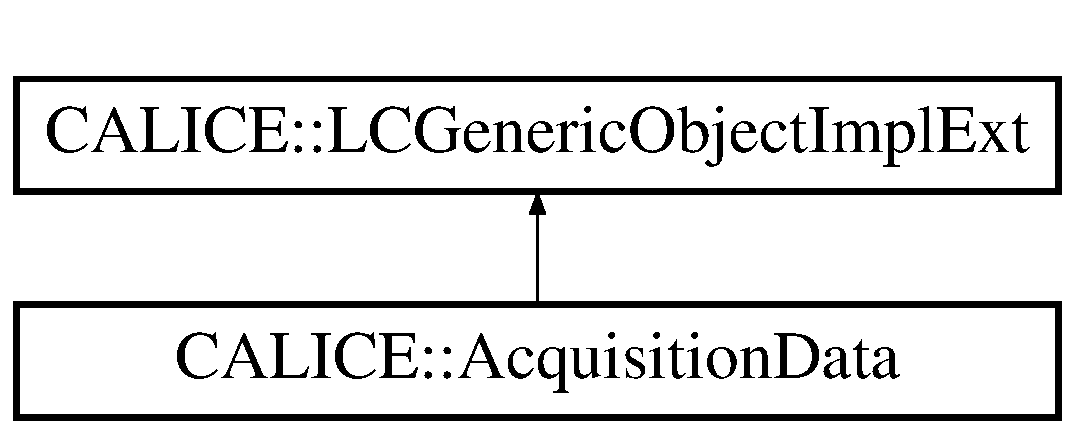
\includegraphics[height=2cm]{classCALICE_1_1AcquisitionData}
\end{center}
\end{figure}
\subsection*{Public Member Functions}
\begin{DoxyCompactItemize}
\item 
{\bf AcquisitionData} (int acquisitionNumberInRun, int acquisitionNumberInConfiguration)\label{classCALICE_1_1AcquisitionData_aa1f1d0bd5bbb808113b480b760b357ef}

\begin{DoxyCompactList}\small\item\em The constructor. \item\end{DoxyCompactList}\item 
{\bf AcquisitionData} (LCObject $\ast$obj)\label{classCALICE_1_1AcquisitionData_a80ddf44bcb6c9070a4774aa640072c46}

\begin{DoxyCompactList}\small\item\em A copy constructor. \item\end{DoxyCompactList}\item 
virtual {\bf $\sim$AcquisitionData} ()\label{classCALICE_1_1AcquisitionData_a03dba78272df176732377006a3e6415c}

\begin{DoxyCompactList}\small\item\em The destructor. \item\end{DoxyCompactList}\item 
{\bf AcquisitionData} \& {\bf setAcquisitionState} (bool acqstate)\label{classCALICE_1_1AcquisitionData_a3f6cf1b411af4a4c73822f3843ce5f9d}

\begin{DoxyCompactList}\small\item\em Sets the acquisition state, start=1, end=0. \item\end{DoxyCompactList}\item 
bool {\bf getAcquisitionState} () const \label{classCALICE_1_1AcquisitionData_afb3d781c28f16db8508bf837864aca54}

\begin{DoxyCompactList}\small\item\em Returns the acquisition state. \item\end{DoxyCompactList}\item 
{\bf AcquisitionData} \& {\bf setTimeInformationSec} (unsigned int timeinfo)
\begin{DoxyCompactList}\small\item\em Set the time information for the given state (in sec), note that the meaning is different for start and end. \item\end{DoxyCompactList}\item 
{\bf AcquisitionData} \& {\bf setTimeInformationMuSec} (unsigned int timeinfo)
\begin{DoxyCompactList}\small\item\em Set the time information for the given state (in sec), note that the meaning is different for start and end. \item\end{DoxyCompactList}\item 
unsigned int {\bf getAcquisitionNumberInRun} ()\label{classCALICE_1_1AcquisitionData_a30dc6e6cf5801240dc672e73703de4f3}

\begin{DoxyCompactList}\small\item\em returns the acquisition number in run \item\end{DoxyCompactList}\item 
unsigned int {\bf getAcquisitionNumberInConfiguration} ()\label{classCALICE_1_1AcquisitionData_a5fdfe4f39cf7c10682eab629243a35f6}

\begin{DoxyCompactList}\small\item\em returns the acquisition number in configuration \item\end{DoxyCompactList}\item 
{\bf AcquisitionData} \& {\bf setEventNumberInfo} (unsigned int evnuminfo)\label{classCALICE_1_1AcquisitionData_a3bab96bafcf9d8badea581d70a9a1778}

\begin{DoxyCompactList}\small\item\em Sets the eventnumber info. \item\end{DoxyCompactList}\item 
unsigned int {\bf getMaxEventNumberInAcquisition} ()\label{classCALICE_1_1AcquisitionData_a4bb9e5f8e2e5e7be1705557db6ff579e}

\begin{DoxyCompactList}\small\item\em returns the maximal number of events in Acquisition \item\end{DoxyCompactList}\item 
unsigned int {\bf getActEventNumberInAcquisition} ()\label{classCALICE_1_1AcquisitionData_a0a3fa8fe5a5a06930597e9b8a3aeb92c}

\begin{DoxyCompactList}\small\item\em returns the actual number of events in Acquisition \item\end{DoxyCompactList}\item 
unsigned int {\bf getMaxAcquisitionTimeSec} ()\label{classCALICE_1_1AcquisitionData_ac3b5becc7288c4cf71b99e9f81c9a564}

\begin{DoxyCompactList}\small\item\em Returns the maximum acquisition time -\/ seconds. \item\end{DoxyCompactList}\item 
unsigned int {\bf getMaxAcquisitionTimeMus} ()\label{classCALICE_1_1AcquisitionData_ab076903057bb3f4a85a144661a3d4223}

\begin{DoxyCompactList}\small\item\em Returns the maximum acquisition time -\/ microseconds. \item\end{DoxyCompactList}\item 
unsigned int {\bf getActAcquisitionTimeSec} ()\label{classCALICE_1_1AcquisitionData_a9c32aed54c8525c4dd143594ebf572e6}

\begin{DoxyCompactList}\small\item\em Returns the actual acquisition time -\/ seconds. \item\end{DoxyCompactList}\item 
unsigned int {\bf getActAcquisitionTimeMus} ()\label{classCALICE_1_1AcquisitionData_a31cc8badfb06afa9ca37db0af726cd27}

\begin{DoxyCompactList}\small\item\em Returns the actual acquisition time -\/ microseconds. \item\end{DoxyCompactList}\item 
{\bf AcquisitionData} \& {\bf setDifInfoPresent} (bool difdatapresent)\label{classCALICE_1_1AcquisitionData_a708b7f09773470d122d82594b2aaf743}

\begin{DoxyCompactList}\small\item\em Set whether there are dif data in the acquisition. \item\end{DoxyCompactList}\item 
bool {\bf getDifDataPresent} () const \label{classCALICE_1_1AcquisitionData_a2f75303f2065483675cc11b596d66fdb}

\begin{DoxyCompactList}\small\item\em Return whether dif data are present in the acquisition. \item\end{DoxyCompactList}\item 
{\bf AcquisitionData} \& {\bf setDifTriggerCounter} (unsigned int triggercounter)\label{classCALICE_1_1AcquisitionData_a47d04ea74eb9197cb24353b1c3a5d9ea}

\begin{DoxyCompactList}\small\item\em Check dif trigger counter at acquisition start and end. \item\end{DoxyCompactList}\item 
unsigned int {\bf getDifTriggerCounter} () const \label{classCALICE_1_1AcquisitionData_a5901280a12cf53272af6ea1a903a5616}

\begin{DoxyCompactList}\small\item\em Return dif trigger counter. \item\end{DoxyCompactList}\item 
{\bf AcquisitionData} \& {\bf setNumberofDifBufferWords} (unsigned int difbufferwords)\label{classCALICE_1_1AcquisitionData_a1a64594b02fe07d2f8c985481a9aedac}

\begin{DoxyCompactList}\small\item\em Check number of dif buffer words. \item\end{DoxyCompactList}\item 
unsigned int {\bf getNumberofDifBufferWords} ()\label{classCALICE_1_1AcquisitionData_a54292d25b63278bcf9d1f62daf623c8e}

\begin{DoxyCompactList}\small\item\em Return number of dif trigger buffer words. \item\end{DoxyCompactList}\item 
const std::string {\bf getTypeName} () const \label{classCALICE_1_1AcquisitionData_af5b75abdb744f5511107bf592abd7564}

\begin{DoxyCompactList}\small\item\em returns the the type name \item\end{DoxyCompactList}\item 
const std::string {\bf getDataDescription} () const \label{classCALICE_1_1AcquisitionData_aaa8b0ef98afc2ebc20bd111802ad96a2}

\begin{DoxyCompactList}\small\item\em returns a brief description of the data stored \item\end{DoxyCompactList}\item 
std::ostream \& {\bf print} (std::ostream \&ostrm)\label{classCALICE_1_1AcquisitionData_aaa13de3cfac3a3f6a4babccb767d7cd9}

\begin{DoxyCompactList}\small\item\em dumps data content \item\end{DoxyCompactList}\end{DoxyCompactItemize}


\subsection{Detailed Description}
Class to store acquisition data info, i.e. acquisiton\# in run, acquisition\# in configuration,max. events in acquistion

Note this is for internal use only \begin{Desc}
\item[{\bf Todo}]should we make a regular userlib class out of it? \end{Desc}
\begin{DoxyAuthor}{Author}
R. P�schl (LAL Orsay) 
\end{DoxyAuthor}
\begin{DoxyDate}{Date}
Feb 27 2006 
\end{DoxyDate}


Definition at line 44 of file AcquisitionData.hh.

\subsection{Member Function Documentation}
\index{CALICE::AcquisitionData@{CALICE::AcquisitionData}!setTimeInformationMuSec@{setTimeInformationMuSec}}
\index{setTimeInformationMuSec@{setTimeInformationMuSec}!CALICE::AcquisitionData@{CALICE::AcquisitionData}}
\subsubsection[{setTimeInformationMuSec}]{\setlength{\rightskip}{0pt plus 5cm}{\bf AcquisitionData}\& CALICE::AcquisitionData::setTimeInformationMuSec (unsigned int {\em timeinfo})\hspace{0.3cm}{\ttfamily  [inline]}}\label{classCALICE_1_1AcquisitionData_a0c06ac70f5934b81cc241b447201b881}


Set the time information for the given state (in sec), note that the meaning is different for start and end. This will be handled further down 

Definition at line 104 of file AcquisitionData.hh.

References CALICE::LCGenericObjectImplExt::obj().\index{CALICE::AcquisitionData@{CALICE::AcquisitionData}!setTimeInformationSec@{setTimeInformationSec}}
\index{setTimeInformationSec@{setTimeInformationSec}!CALICE::AcquisitionData@{CALICE::AcquisitionData}}
\subsubsection[{setTimeInformationSec}]{\setlength{\rightskip}{0pt plus 5cm}{\bf AcquisitionData}\& CALICE::AcquisitionData::setTimeInformationSec (unsigned int {\em timeinfo})\hspace{0.3cm}{\ttfamily  [inline]}}\label{classCALICE_1_1AcquisitionData_a42d0b8ad6f9ba2bfddb3af8b2683dfa5}


Set the time information for the given state (in sec), note that the meaning is different for start and end. This will be handled further down 

Definition at line 97 of file AcquisitionData.hh.

References CALICE::LCGenericObjectImplExt::obj().

The documentation for this class was generated from the following files:\begin{DoxyCompactItemize}
\item 
AcquisitionData.hh\item 
AcquisitionData.cc\end{DoxyCompactItemize}

\section{CALICE::AdcBlock Class Reference}
\label{classCALICE_1_1AdcBlock}\index{CALICE::AdcBlock@{CALICE::AdcBlock}}


Class for the ADC Data as acquired by the \doxyref{CALICE}{p.}{namespaceCALICE} DAQ.  


{\ttfamily \#include $<$AdcBlock.hh$>$}\subsection*{Public Member Functions}
\begin{DoxyCompactItemize}
\item 
{\bf AdcBlock} (int boardID, int label, int Fe, int Imul, const AdcBlockArray \&adcBlock, int status)\label{classCALICE_1_1AdcBlock_a6cfc92f7005861497f3da19929b3305c}

\begin{DoxyCompactList}\small\item\em Convenient c'tor. \item\end{DoxyCompactList}\item 
{\bf AdcBlock} (LCObject $\ast$obj)\label{classCALICE_1_1AdcBlock_ab78d098d531e821e759f4f82db0942de}

\begin{DoxyCompactList}\small\item\em 'Copy constructor' needed to interpret LCCollection read from file/database. \item\end{DoxyCompactList}\item 
virtual {\bf $\sim$AdcBlock} ()\label{classCALICE_1_1AdcBlock_af3dc2bf5b9ef534971a256f5b15d51dd}

\begin{DoxyCompactList}\small\item\em Important for memory handling. \item\end{DoxyCompactList}\item 
unsigned int {\bf getBoardID} () const \label{classCALICE_1_1AdcBlock_a9a8352cd4be0a403b477ac602217ca3a}

\begin{DoxyCompactList}\small\item\em get the board id. \item\end{DoxyCompactList}\item 
unsigned {\bf getElecChannel} (int) const 
\begin{DoxyCompactList}\small\item\em the class interface: \item\end{DoxyCompactList}\item 
short {\bf getAdcVal} (int i) const \label{classCALICE_1_1AdcBlock_a3c78cb752efdb526d69c64f17c880616}

\begin{DoxyCompactList}\small\item\em and the actual ADC calue \item\end{DoxyCompactList}\item 
short {\bf getBoardFrontEnd} () const \label{classCALICE_1_1AdcBlock_aeba50c8fb0cb56a399027c1a24254d96}

\begin{DoxyCompactList}\small\item\em Information on the FE chip the data was received. \item\end{DoxyCompactList}\item 
short {\bf getMultiplexPosition} () const \label{classCALICE_1_1AdcBlock_a2978073ea8348f69e62bb0cbe15cab10}

\begin{DoxyCompactList}\small\item\em and the position within the series of transmissions \item\end{DoxyCompactList}\item 
short {\bf getCrateID} () const \label{classCALICE_1_1AdcBlock_a6bcccdc816b7c0cf695a7853071ffe6f}

\begin{DoxyCompactList}\small\item\em Some general information on the board on which the data was received on the Crate Id. \item\end{DoxyCompactList}\item 
short {\bf getSlotID} () const \label{classCALICE_1_1AdcBlock_a13560d4d9931ac08b13052580f67969a}

\begin{DoxyCompactList}\small\item\em on the Slot Id \item\end{DoxyCompactList}\item 
short {\bf getBoardComponentNumber} () const \label{classCALICE_1_1AdcBlock_ab782b69f80d4226d89a8b98221935c1b}

\begin{DoxyCompactList}\small\item\em on the BoardComponent Number \item\end{DoxyCompactList}\item 
short {\bf getRecordLabel} () const \label{classCALICE_1_1AdcBlock_af22b4a1cedb615b08899904eed3725bc}

\begin{DoxyCompactList}\small\item\em on the Board Label \item\end{DoxyCompactList}\item 
short {\bf getTransmissionStatus} () const \label{classCALICE_1_1AdcBlock_a8e9c8c2fe91eeed4f202aee8497c1854}

\begin{DoxyCompactList}\small\item\em Transmission of data from piggy back to FE. \item\end{DoxyCompactList}\item 
void {\bf print} (std::ostream \&os, int)\label{classCALICE_1_1AdcBlock_a6bd9f304b2fada336341073e07c41f13}

\begin{DoxyCompactList}\small\item\em Convenient print method. \item\end{DoxyCompactList}\item 
const std::string {\bf getTypeName} () const \label{classCALICE_1_1AdcBlock_aeba86a15ac0ad04d3564bae5aec911fb}

\begin{DoxyCompactList}\small\item\em Return the type of the class. \item\end{DoxyCompactList}\item 
const std::string {\bf getDataDescription} () const \label{classCALICE_1_1AdcBlock_a0f2e508485b4214ab454b72fc0c591ed}

\begin{DoxyCompactList}\small\item\em Return a brief description of the data members. \item\end{DoxyCompactList}\end{DoxyCompactItemize}


\subsection{Detailed Description}
Class for the ADC Data as acquired by the \doxyref{CALICE}{p.}{namespaceCALICE} DAQ. The class reflects that the data are received in chunks of 12 ADC's within a series of 18 transmissions (multiplexing).

ADC data are stored together with the indices of the board by which they were received, the FE (0-\/8) and their position within the multiplexed series (0-\/17). The class provides interface functions to get the adc value within the adc block as well as an associated electronic channel id: ElecChannelID = CrateID , SlotID, FE, Multipl., ADC\_\-i: Bit: 31-\/24 , 23-\/16, 15-\/12, 11-\/4 , 3-\/0 \begin{DoxyAuthor}{Author}
R. P�schl DESY 
\end{DoxyAuthor}
\begin{DoxyDate}{Date}
Mar 5 2005 
\end{DoxyDate}


Definition at line 34 of file AdcBlock.hh.

\subsection{Member Function Documentation}
\index{CALICE::AdcBlock@{CALICE::AdcBlock}!getElecChannel@{getElecChannel}}
\index{getElecChannel@{getElecChannel}!CALICE::AdcBlock@{CALICE::AdcBlock}}
\subsubsection[{getElecChannel}]{\setlength{\rightskip}{0pt plus 5cm}unsigned CALICE::AdcBlock::getElecChannel (int {\em i}) const}\label{classCALICE_1_1AdcBlock_af03eee5e03977fbab76d5fc98d113ef8}


the class interface: get electronic channel id assigned to the adc 

Definition at line 9 of file AdcBlock.cc.

Referenced by print().

The documentation for this class was generated from the following files:\begin{DoxyCompactItemize}
\item 
AdcBlock.hh\item 
AdcBlock.cc\end{DoxyCompactItemize}

\section{CALICE::Ahc2Calibrations Class Reference}
\label{classCALICE_1_1Ahc2Calibrations}\index{CALICE::Ahc2Calibrations@{CALICE::Ahc2Calibrations}}


storing all informations necessary to calibrate a HBU SiPM read channel  


{\ttfamily \#include $<$Ahc2Calibrations.hh$>$}\subsection*{Public Member Functions}
\begin{DoxyCompactItemize}
\item 
{\bfseries Ahc2Calibrations} ({\bf LinearFitCompound} $\ast$MIP, {\bf LinearFitCompound} $\ast$gain, {\bf SimpleValue} $\ast$pedestal, {\bf SimpleValue} $\ast$interCalibration, {\bf SimpleValue} $\ast$interCalibrationPhysicsCalib, {\bf SimpleValue} $\ast$temperature, {\bf SaturationParameters} $\ast$saturation, {\bf SimpleValueVector} $\ast$timeSlopesCalibration, {\bf SimpleValueVector} $\ast$timePedestalCalibration, const int status, const int cellID, const std::string \&cellIDEncoding)\label{classCALICE_1_1Ahc2Calibrations_ad60d53f4b2f81bfb0cc8258a57039038}

\item 
{\bf LinearFitCompound} $\ast$ {\bfseries getMIP} () const \label{classCALICE_1_1Ahc2Calibrations_a8fdd3c513f5bb8ff484ece6173dbf3fe}

\item 
{\bf LinearFitCompound} $\ast$ {\bfseries getGain} () const \label{classCALICE_1_1Ahc2Calibrations_ab4a252f2e7589fd8429a65774181ecb3}

\item 
{\bf SimpleValue} $\ast$ {\bfseries getPedestal} () const \label{classCALICE_1_1Ahc2Calibrations_ae1c09b266458a55af0f854cbd714231c}

\item 
{\bf SimpleValue} $\ast$ {\bfseries getInterCalibration} () const \label{classCALICE_1_1Ahc2Calibrations_a8edc2b5e2d253116996be42c6c7cd90c}

\item 
{\bf SimpleValue} $\ast$ {\bfseries getPhysicsCalibIC} () const \label{classCALICE_1_1Ahc2Calibrations_abc1a937aac4a27234ac474901a847624}

\item 
{\bf SimpleValue} $\ast$ {\bfseries getTemperature} () const \label{classCALICE_1_1Ahc2Calibrations_a0169760750c84e6341f5293e8347cf75}

\item 
{\bf SaturationParameters} $\ast$ {\bfseries getSaturation} () const \label{classCALICE_1_1Ahc2Calibrations_acfbbab2fcfc1353175bf2196512122a5}

\item 
{\bf SimpleValueVector} $\ast$ {\bfseries getTimeSlopes} () const \label{classCALICE_1_1Ahc2Calibrations_a2d565ca0cdc228535d932845c2e25bc5}

\item 
{\bf SimpleValueVector} $\ast$ {\bfseries getTimePedestal} () const \label{classCALICE_1_1Ahc2Calibrations_a3c95865d6b09e0047a2fa36d98327a73}

\item 
int {\bfseries getStatus} () const \label{classCALICE_1_1Ahc2Calibrations_abd138930b5b67cda32960a1e5805369f}

\item 
int {\bfseries getCellID} () const \label{classCALICE_1_1Ahc2Calibrations_a863df224a883b4075531d5718a309959}

\item 
const std::string \& {\bfseries getCellIDEncoding} () const \label{classCALICE_1_1Ahc2Calibrations_a912aefba37f34f874a3c05ae029d9f10}

\item 
void {\bfseries setMIP} ({\bf LinearFitCompound} $\ast$MIP)\label{classCALICE_1_1Ahc2Calibrations_a579397bf370b64b210647a449fece2cb}

\item 
void {\bfseries setGain} ({\bf LinearFitCompound} $\ast$gain)\label{classCALICE_1_1Ahc2Calibrations_ab6cad8fd192851c21edbbd6aa1814f68}

\item 
void {\bfseries setPedestal} ({\bf SimpleValue} $\ast$pedestal)\label{classCALICE_1_1Ahc2Calibrations_a8b2e58c97f7e5b5a25fd07d66333d95d}

\item 
void {\bfseries setInterCalibration} ({\bf SimpleValue} $\ast$interCalibration)\label{classCALICE_1_1Ahc2Calibrations_a7a5db8ef5f4c3f2aab84889b54c15852}

\item 
void {\bfseries setPhysicsCalibIC} ({\bf SimpleValue} $\ast$interCalibrationPhysicsCalib)\label{classCALICE_1_1Ahc2Calibrations_ac83d32c7dac04831bd8890c357e2e49c}

\item 
void {\bfseries setTemperature} ({\bf SimpleValue} $\ast$temperature)\label{classCALICE_1_1Ahc2Calibrations_ae1409d9eb74bc38bbce60f13231df61d}

\item 
void {\bfseries setSaturation} ({\bf SaturationParameters} $\ast$param)\label{classCALICE_1_1Ahc2Calibrations_acd5284f9adbcd950fe3caa9244495a34}

\item 
void {\bfseries setTimeSlopes} ({\bf SimpleValueVector} $\ast$timeSlopes)\label{classCALICE_1_1Ahc2Calibrations_a673f9d436e10789805e539773b5a4887}

\item 
void {\bfseries setTimePedestal} ({\bf SimpleValueVector} $\ast$timePedestal)\label{classCALICE_1_1Ahc2Calibrations_ac078790dda2218d2db7b7a7417167883}

\item 
void {\bfseries setStatus} (const int status)\label{classCALICE_1_1Ahc2Calibrations_ad5435a2ccdfa548e16c8c7a6dbdacb77}

\item 
void {\bfseries setCellID} (const int cellID)\label{classCALICE_1_1Ahc2Calibrations_a34bbc74589d8a3e41719c5ce3cff3a38}

\item 
void {\bfseries setCellIDEncoding} (const std::string \&encoding)\label{classCALICE_1_1Ahc2Calibrations_a09ce017f8db987840a98331781425d68}

\end{DoxyCompactItemize}
\subsection*{Private Attributes}
\begin{DoxyCompactItemize}
\item 
{\bf LinearFitCompound} $\ast$ {\bfseries \_\-gain}\label{classCALICE_1_1Ahc2Calibrations_a03eefbf76823ac538ac161116c721094}

\item 
{\bf LinearFitCompound} $\ast$ {\bfseries \_\-MIP}\label{classCALICE_1_1Ahc2Calibrations_a62f955858c113f4d74839b775431573f}

\item 
{\bf SimpleValue} $\ast$ {\bfseries \_\-pedestal}\label{classCALICE_1_1Ahc2Calibrations_a4efe9ef32165ddb8b060e1cea599662c}

\item 
{\bf SimpleValue} $\ast$ {\bfseries \_\-interCalibration}\label{classCALICE_1_1Ahc2Calibrations_ae4efcf3a0b9a4f68a0b0bec543f1127f}

\item 
{\bf SimpleValue} $\ast$ {\bfseries \_\-interCalibrationPhysicsCalib}\label{classCALICE_1_1Ahc2Calibrations_a857c20a5260ad72e67fd331b714e95e5}

\item 
{\bf SimpleValue} $\ast$ {\bfseries \_\-temperature}\label{classCALICE_1_1Ahc2Calibrations_aa3af368bb355aedaa207832852ebf38a}

\item 
{\bf SaturationParameters} $\ast$ {\bfseries \_\-saturation}\label{classCALICE_1_1Ahc2Calibrations_af91d92efebefb744991268c919b2f8c6}

\item 
{\bf SimpleValueVector} $\ast$ {\bfseries \_\-timeSlopesCalibration}\label{classCALICE_1_1Ahc2Calibrations_a07e277795a54bda83dd8b3d866b7bdf7}

\item 
{\bf SimpleValueVector} $\ast$ {\bfseries \_\-timePedestalCalibration}\label{classCALICE_1_1Ahc2Calibrations_af5d78742591d17ef4f92c5364b5764d0}

\item 
int {\bfseries \_\-status}\label{classCALICE_1_1Ahc2Calibrations_a92a7eab19aa5cc8bebdfdcd4989f17b3}

\item 
int {\bfseries \_\-cellID}\label{classCALICE_1_1Ahc2Calibrations_a444c186f7f53950fb4a17759adc2fc87}

\item 
std::string {\bfseries \_\-cellIDEncoding}\label{classCALICE_1_1Ahc2Calibrations_a37a85e6102734162295d0e187ea19ff5}

\end{DoxyCompactItemize}


\subsection{Detailed Description}
storing all informations necessary to calibrate a HBU SiPM read channel This class is meant as central holder of all necessary informations to calibrate a HBU SiPM. Currently, following informations are stored: \begin{DoxyItemize}
\item {\ttfamily MIP} calibration in form of a {\bfseries \doxyref{LinearFitResult}{p.}{classCALICE_1_1LinearFitResult}} \item {\ttfamily gain} calibration in form of a {\bfseries \doxyref{LinearFitResult}{p.}{classCALICE_1_1LinearFitResult}} \item {\ttfamily pedestal} calibration in form of a {\bfseries \doxyref{SimpleValue}{p.}{classCALICE_1_1SimpleValue}} \item {\ttfamily temperature} calibration in form of a {\bfseries \doxyref{SimpleValue}{p.}{classCALICE_1_1SimpleValue}} \item {\ttfamily inter} {\ttfamily calibration} in form of a {\bfseries \doxyref{SimpleValue}{p.}{classCALICE_1_1SimpleValue}} \item {\ttfamily inter} {\ttfamily calibration} Physics Calib in form of a {\bfseries \doxyref{SimpleValue}{p.}{classCALICE_1_1SimpleValue}} \item {\ttfamily saturation} {\ttfamily parameters} {\ttfamily in} form of a {\bfseries \doxyref{SaturationParameters}{p.}{classCALICE_1_1SaturationParameters}} \item {\ttfamily time} slopes {\ttfamily parameters} {\ttfamily in} form of a {\bfseries \doxyref{SimpleValueVector}{p.}{classCALICE_1_1SimpleValueVector}} \item {\ttfamily time} pedestal {\ttfamily parameters} {\ttfamily in} form of a {\bfseries \doxyref{SimpleValueVector}{p.}{classCALICE_1_1SimpleValueVector}} \item {\ttfamily status} in form of an {\bfseries integer} \end{DoxyItemize}
\begin{DoxyAuthor}{Author}
{\tt Shaojun.lu@desy.de} 
\end{DoxyAuthor}
\begin{DoxyVersion}{Version}
0.1 
\end{DoxyVersion}
\begin{DoxyDate}{Date}
Feburary 2013 
\end{DoxyDate}


Definition at line 33 of file Ahc2Calibrations.hh.

The documentation for this class was generated from the following files:\begin{DoxyCompactItemize}
\item 
Ahc2Calibrations.hh\item 
Ahc2Calibrations.cc\end{DoxyCompactItemize}

\section{CALICE::Ahc2CalibrationStatusBits Class Reference}
\label{classCALICE_1_1Ahc2CalibrationStatusBits}\index{CALICE::Ahc2CalibrationStatusBits@{CALICE::Ahc2CalibrationStatusBits}}


Bit set to describe the Ahc2 Calibration Status.  


{\ttfamily \#include $<$Ahc2CalibrationStatusBits.hh$>$}Inheritance diagram for CALICE::Ahc2CalibrationStatusBits::\begin{figure}[H]
\begin{center}
\leavevmode
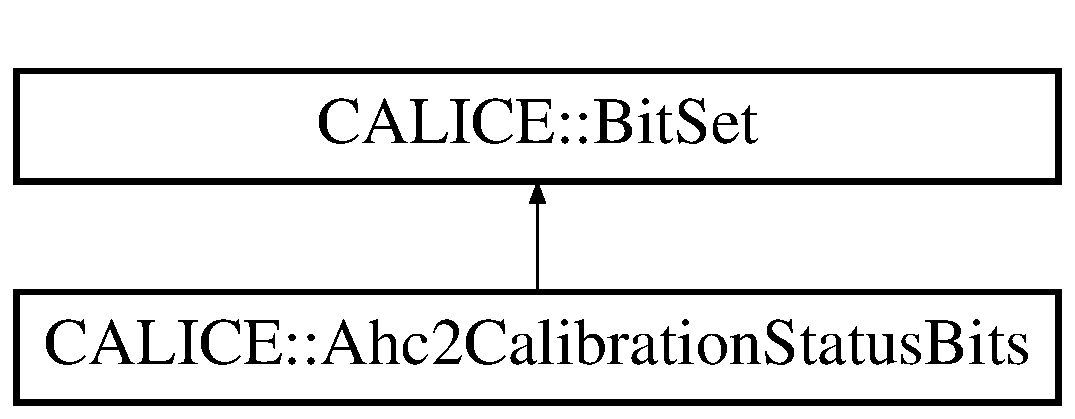
\includegraphics[height=2cm]{classCALICE_1_1Ahc2CalibrationStatusBits}
\end{center}
\end{figure}
\subsection*{Public Member Functions}
\begin{DoxyCompactItemize}
\item 
{\bf Ahc2CalibrationStatusBits} ()
\begin{DoxyCompactList}\small\item\em standard constructor \item\end{DoxyCompactList}\item 
{\bf Ahc2CalibrationStatusBits} (const int value)
\begin{DoxyCompactList}\small\item\em constructor with initialisaton of the the bits \item\end{DoxyCompactList}\item 
bool {\bfseries isDead} () const \label{classCALICE_1_1Ahc2CalibrationStatusBits_ac0d15dd4f791b91c9c6ad5fe41fd6cc3}

\item 
bool {\bfseries noPedestal} () const \label{classCALICE_1_1Ahc2CalibrationStatusBits_a6edc0dfbb241566136c21ab01669fc51}

\item 
bool {\bfseries noTemperature} () const \label{classCALICE_1_1Ahc2CalibrationStatusBits_a9fb04b1b5428592afefa219ecf9aec49}

\item 
bool {\bfseries isNewITEP} () const \label{classCALICE_1_1Ahc2CalibrationStatusBits_a6fb3027bf68829d150668f0184423ecd}

\item 
bool {\bfseries MIPConstantIsDefault} () const \label{classCALICE_1_1Ahc2CalibrationStatusBits_af11386a9a08c65042522c4b2af4f9f6f}

\item 
bool {\bfseries MIPSlopeIsDefault} () const \label{classCALICE_1_1Ahc2CalibrationStatusBits_a50b4fe7b0aa00e0483bb59a2d99af59f}

\item 
bool {\bfseries gainConstantIsDefault} () const \label{classCALICE_1_1Ahc2CalibrationStatusBits_a7098ed6fd937b62c040c929eb40682d1}

\item 
bool {\bfseries gainSlopeIsDefault} () const \label{classCALICE_1_1Ahc2CalibrationStatusBits_a4bb22c8217cdf4b6b0ac9c181aedb3a3}

\item 
bool {\bfseries interCalibrationIsDefault} () const \label{classCALICE_1_1Ahc2CalibrationStatusBits_aa90445a6de7f1f35b3e8e1ffe34299a9}

\item 
bool {\bfseries PhysicsCalibICIsDefault} () const \label{classCALICE_1_1Ahc2CalibrationStatusBits_a5cee89c4a70a9e196bae203818920bc4}

\item 
bool {\bfseries saturationParametersIsDefault} () const \label{classCALICE_1_1Ahc2CalibrationStatusBits_a838584c262cfbccea7969744e968e563}

\item 
bool {\bfseries TimeSlopesParametersIsDefault} () const \label{classCALICE_1_1Ahc2CalibrationStatusBits_a84bb230b2a5a83cc168640aef3675027}

\item 
bool {\bfseries TimePedestalParametersIsDefault} () const \label{classCALICE_1_1Ahc2CalibrationStatusBits_a1f1ec182447b2628a06d9b1f287cd9a1}

\item 
bool {\bfseries hasDefault} () const \label{classCALICE_1_1Ahc2CalibrationStatusBits_abc660f877930fa42c2e8527dcff5d2d7}

\item 
bool {\bfseries MIPConstantIsScaled} () const \label{classCALICE_1_1Ahc2CalibrationStatusBits_a7c8965a803ecec5750d1c230d3276ce9}

\item 
bool {\bfseries MIPSlopeIsScaled} () const \label{classCALICE_1_1Ahc2CalibrationStatusBits_a5ab7245b3e09f28776a5456796e7fa2e}

\item 
bool {\bfseries gainConstantIsScaled} () const \label{classCALICE_1_1Ahc2CalibrationStatusBits_a4590015de61eadec69155b6f052785ef}

\item 
bool {\bfseries gainSlopeIsScaled} () const \label{classCALICE_1_1Ahc2CalibrationStatusBits_a0f661aabae4ebbc614e5cd64f5494997}

\item 
bool {\bfseries interCalibrationIsScaled} () const \label{classCALICE_1_1Ahc2CalibrationStatusBits_a05d6c638e0e7f499f8b767deba52b7ef}

\item 
bool {\bfseries PhysicsCalibICIsScaled} () const \label{classCALICE_1_1Ahc2CalibrationStatusBits_a9cd5210e7e5a264e30965e2014d9eedc}

\item 
bool {\bfseries hasScaled} () const \label{classCALICE_1_1Ahc2CalibrationStatusBits_a7722b3dc5a233bcb4390f62f809dd56c}

\item 
void {\bfseries setDead} (const bool state=true)\label{classCALICE_1_1Ahc2CalibrationStatusBits_a7086d3e5eb96292e47cd896457986780}

\item 
void {\bfseries setNoPedestal} (const bool state=true)\label{classCALICE_1_1Ahc2CalibrationStatusBits_a759b14ec17dfa8266058ee01400fec4e}

\item 
void {\bfseries setNoTemperature} (const bool state=true)\label{classCALICE_1_1Ahc2CalibrationStatusBits_aa3c37fe71a8a3727699dda63f145d08e}

\item 
void {\bfseries setisNewITEP} (const bool state=true)\label{classCALICE_1_1Ahc2CalibrationStatusBits_a618d44185909927e61bf308b71ab3f02}

\item 
void {\bfseries setMIPConstantDefault} (const bool state=true)\label{classCALICE_1_1Ahc2CalibrationStatusBits_a563abd517939b634e2d4a032476c5f50}

\item 
void {\bfseries setMIPSlopeDefault} (const bool state=true)\label{classCALICE_1_1Ahc2CalibrationStatusBits_a93d2fb3dbcae45735a46faaea352c39b}

\item 
void {\bfseries setGainConstantDefault} (const bool state=true)\label{classCALICE_1_1Ahc2CalibrationStatusBits_ab4b50418d9b99b263842832f41cf6d8f}

\item 
void {\bfseries setGainSlopeDefault} (const bool state=true)\label{classCALICE_1_1Ahc2CalibrationStatusBits_a8a9da4c25b8317896497ec216f831fc6}

\item 
void {\bfseries setInterCalibrationDefault} (const bool state=true)\label{classCALICE_1_1Ahc2CalibrationStatusBits_adb01ce4e46929b52e7fb89dcc8e0d89b}

\item 
void {\bfseries setPhysicsCalibICDefault} (const bool state=true)\label{classCALICE_1_1Ahc2CalibrationStatusBits_a7b51b16ade7fdf0803b968e41e94303e}

\item 
void {\bfseries setSaturationParametersDefault} (const bool state=true)\label{classCALICE_1_1Ahc2CalibrationStatusBits_a215a322f8475633417f9727e1f073908}

\item 
void {\bfseries setTimeSlopesParametersDefault} (const bool state=true)\label{classCALICE_1_1Ahc2CalibrationStatusBits_a50e4cfea2375a925be6e50fe82eda241}

\item 
void {\bfseries setTimePedestalParametersDefault} (const bool state=true)\label{classCALICE_1_1Ahc2CalibrationStatusBits_a8f62dcfae9efb8ab82b18f90448aec7a}

\item 
void {\bfseries setMIPConstantScaled} (const bool state=true)\label{classCALICE_1_1Ahc2CalibrationStatusBits_a7b90ee374016c59fe0931a1e42840941}

\item 
void {\bfseries setMIPSlopeScaled} (const bool state=true)\label{classCALICE_1_1Ahc2CalibrationStatusBits_a2e2221cf01d5766f3f3ff1d66fc9364a}

\item 
void {\bfseries setGainConstantScaled} (const bool state=true)\label{classCALICE_1_1Ahc2CalibrationStatusBits_ae6dcfafd7074e5915ae7adb2e7c2101d}

\item 
void {\bfseries setGainSlopeScaled} (const bool state=true)\label{classCALICE_1_1Ahc2CalibrationStatusBits_a7c8db965152f0f13fb2d0b2278136288}

\item 
void {\bfseries setInterCalibrationScaled} (const bool state=true)\label{classCALICE_1_1Ahc2CalibrationStatusBits_ad918faf4d0f89479592661f385559ec6}

\item 
void {\bfseries setPhysicsCalibICScaled} (const bool state=true)\label{classCALICE_1_1Ahc2CalibrationStatusBits_a214becc89abb9ebfaa913884f848d59c}

\end{DoxyCompactItemize}
\subsection*{Protected Types}
\begin{DoxyCompactItemize}
\item 
enum {\bf EAhc2CalibrationStatusBitNo} \{ \par
{\bf kIsDead}, 
{\bf kNoPedestal}, 
{\bf kNoTemperature}, 
{\bf kisNewITEP}, 
\par
{\bf kMIPConstantIsDefault}, 
{\bf kMIPSlopeIsDefault}, 
{\bf kGainConstantIsDefault}, 
{\bf kGainSlopeIsDefault}, 
\par
{\bf kInterCalibrationIsDefault}, 
{\bf kPhysicsCalibICIsDefault}, 
{\bf kSaturationParametersIsDefault}, 
{\bf kTimeSlopesParametersIsDefault}, 
\par
{\bf kTimePedestalParametersIsDefault}, 
{\bf kMIPConstantIsScaled}, 
{\bf kMIPSlopeIsScaled}, 
{\bf kGainConstantIsScaled}, 
\par
{\bf kGainSlopeIsScaled}, 
{\bf kInterCalibrationIsScaled}, 
{\bf kPhysicsCalibICIsScaled}, 
{\bfseries kNumberOfBits}
 \}
\end{DoxyCompactItemize}


\subsection{Detailed Description}
Bit set to describe the Ahc2 Calibration Status. \begin{DoxyAuthor}{Author}
E.Brianne 
\end{DoxyAuthor}
\begin{DoxyDate}{Date}
Novemeber 2015 
\end{DoxyDate}
\begin{DoxyVersion}{Version}
1.0 
\end{DoxyVersion}


Definition at line 16 of file Ahc2CalibrationStatusBits.hh.

\subsection{Member Enumeration Documentation}
\index{CALICE::Ahc2CalibrationStatusBits@{CALICE::Ahc2CalibrationStatusBits}!EAhc2CalibrationStatusBitNo@{EAhc2CalibrationStatusBitNo}}
\index{EAhc2CalibrationStatusBitNo@{EAhc2CalibrationStatusBitNo}!CALICE::Ahc2CalibrationStatusBits@{CALICE::Ahc2CalibrationStatusBits}}
\subsubsection[{EAhc2CalibrationStatusBitNo}]{\setlength{\rightskip}{0pt plus 5cm}enum {\bf CALICE::Ahc2CalibrationStatusBits::EAhc2CalibrationStatusBitNo}\hspace{0.3cm}{\ttfamily  [protected]}}\label{classCALICE_1_1Ahc2CalibrationStatusBits_ad3344194d3554ee4db5684dcffc0125a}
\begin{Desc}
\item[Enumerator: ]\par
\begin{description}
\index{kIsDead@{kIsDead}!CALICE::Ahc2CalibrationStatusBits@{CALICE::Ahc2CalibrationStatusBits}}\index{CALICE::Ahc2CalibrationStatusBits@{CALICE::Ahc2CalibrationStatusBits}!kIsDead@{kIsDead}}\item[{\em 
kIsDead\label{classCALICE_1_1Ahc2CalibrationStatusBits_ad3344194d3554ee4db5684dcffc0125aa7e34ebc884839af14f752026f2e0760a}
}]this cell is flagged dead \index{kNoPedestal@{kNoPedestal}!CALICE::Ahc2CalibrationStatusBits@{CALICE::Ahc2CalibrationStatusBits}}\index{CALICE::Ahc2CalibrationStatusBits@{CALICE::Ahc2CalibrationStatusBits}!kNoPedestal@{kNoPedestal}}\item[{\em 
kNoPedestal\label{classCALICE_1_1Ahc2CalibrationStatusBits_ad3344194d3554ee4db5684dcffc0125aae03d7c52fdaa22d8868acd451b9f36d8}
}]no pedestal value available \index{kNoTemperature@{kNoTemperature}!CALICE::Ahc2CalibrationStatusBits@{CALICE::Ahc2CalibrationStatusBits}}\index{CALICE::Ahc2CalibrationStatusBits@{CALICE::Ahc2CalibrationStatusBits}!kNoTemperature@{kNoTemperature}}\item[{\em 
kNoTemperature\label{classCALICE_1_1Ahc2CalibrationStatusBits_ad3344194d3554ee4db5684dcffc0125aa607335442ed069c70b528de9962b81ee}
}]no temperature value available \index{kisNewITEP@{kisNewITEP}!CALICE::Ahc2CalibrationStatusBits@{CALICE::Ahc2CalibrationStatusBits}}\index{CALICE::Ahc2CalibrationStatusBits@{CALICE::Ahc2CalibrationStatusBits}!kisNewITEP@{kisNewITEP}}\item[{\em 
kisNewITEP\label{classCALICE_1_1Ahc2CalibrationStatusBits_ad3344194d3554ee4db5684dcffc0125aac117f122621d0afb9f8877dba5a0aa02}
}]is a new ITEP Tile \index{kMIPConstantIsDefault@{kMIPConstantIsDefault}!CALICE::Ahc2CalibrationStatusBits@{CALICE::Ahc2CalibrationStatusBits}}\index{CALICE::Ahc2CalibrationStatusBits@{CALICE::Ahc2CalibrationStatusBits}!kMIPConstantIsDefault@{kMIPConstantIsDefault}}\item[{\em 
kMIPConstantIsDefault\label{classCALICE_1_1Ahc2CalibrationStatusBits_ad3344194d3554ee4db5684dcffc0125aa63fd30db886fb78bc405e0b01561ecc3}
}]the default MIP constant was used \index{kMIPSlopeIsDefault@{kMIPSlopeIsDefault}!CALICE::Ahc2CalibrationStatusBits@{CALICE::Ahc2CalibrationStatusBits}}\index{CALICE::Ahc2CalibrationStatusBits@{CALICE::Ahc2CalibrationStatusBits}!kMIPSlopeIsDefault@{kMIPSlopeIsDefault}}\item[{\em 
kMIPSlopeIsDefault\label{classCALICE_1_1Ahc2CalibrationStatusBits_ad3344194d3554ee4db5684dcffc0125aa237f11a760410e8f1071c4dc583df52b}
}]the default MIP slope was used \index{kGainConstantIsDefault@{kGainConstantIsDefault}!CALICE::Ahc2CalibrationStatusBits@{CALICE::Ahc2CalibrationStatusBits}}\index{CALICE::Ahc2CalibrationStatusBits@{CALICE::Ahc2CalibrationStatusBits}!kGainConstantIsDefault@{kGainConstantIsDefault}}\item[{\em 
kGainConstantIsDefault\label{classCALICE_1_1Ahc2CalibrationStatusBits_ad3344194d3554ee4db5684dcffc0125aad9cd362824e536d4b55b6373817c92db}
}]the default gain constant was used \index{kGainSlopeIsDefault@{kGainSlopeIsDefault}!CALICE::Ahc2CalibrationStatusBits@{CALICE::Ahc2CalibrationStatusBits}}\index{CALICE::Ahc2CalibrationStatusBits@{CALICE::Ahc2CalibrationStatusBits}!kGainSlopeIsDefault@{kGainSlopeIsDefault}}\item[{\em 
kGainSlopeIsDefault\label{classCALICE_1_1Ahc2CalibrationStatusBits_ad3344194d3554ee4db5684dcffc0125aa217bfa9d316f56996b6780ef43784ee7}
}]the default gain slope was used \index{kInterCalibrationIsDefault@{kInterCalibrationIsDefault}!CALICE::Ahc2CalibrationStatusBits@{CALICE::Ahc2CalibrationStatusBits}}\index{CALICE::Ahc2CalibrationStatusBits@{CALICE::Ahc2CalibrationStatusBits}!kInterCalibrationIsDefault@{kInterCalibrationIsDefault}}\item[{\em 
kInterCalibrationIsDefault\label{classCALICE_1_1Ahc2CalibrationStatusBits_ad3344194d3554ee4db5684dcffc0125aa86728ec4fb7915a15e4893ebc8aef3c1}
}]the default inter-\/calibration constant was used \index{kPhysicsCalibICIsDefault@{kPhysicsCalibICIsDefault}!CALICE::Ahc2CalibrationStatusBits@{CALICE::Ahc2CalibrationStatusBits}}\index{CALICE::Ahc2CalibrationStatusBits@{CALICE::Ahc2CalibrationStatusBits}!kPhysicsCalibICIsDefault@{kPhysicsCalibICIsDefault}}\item[{\em 
kPhysicsCalibICIsDefault\label{classCALICE_1_1Ahc2CalibrationStatusBits_ad3344194d3554ee4db5684dcffc0125aade97e2ae931cae9636c5395a8d612253}
}]the default inter-\/calibration physics/calib constant was used \index{kSaturationParametersIsDefault@{kSaturationParametersIsDefault}!CALICE::Ahc2CalibrationStatusBits@{CALICE::Ahc2CalibrationStatusBits}}\index{CALICE::Ahc2CalibrationStatusBits@{CALICE::Ahc2CalibrationStatusBits}!kSaturationParametersIsDefault@{kSaturationParametersIsDefault}}\item[{\em 
kSaturationParametersIsDefault\label{classCALICE_1_1Ahc2CalibrationStatusBits_ad3344194d3554ee4db5684dcffc0125aacdd3ebd3a6ab6e06c921564c398c3140}
}]the default saturation parameters was used \index{kTimeSlopesParametersIsDefault@{kTimeSlopesParametersIsDefault}!CALICE::Ahc2CalibrationStatusBits@{CALICE::Ahc2CalibrationStatusBits}}\index{CALICE::Ahc2CalibrationStatusBits@{CALICE::Ahc2CalibrationStatusBits}!kTimeSlopesParametersIsDefault@{kTimeSlopesParametersIsDefault}}\item[{\em 
kTimeSlopesParametersIsDefault\label{classCALICE_1_1Ahc2CalibrationStatusBits_ad3344194d3554ee4db5684dcffc0125aa364d9be2e09985c9291aeb432b527f3f}
}]the default time slopes parameters was used \index{kTimePedestalParametersIsDefault@{kTimePedestalParametersIsDefault}!CALICE::Ahc2CalibrationStatusBits@{CALICE::Ahc2CalibrationStatusBits}}\index{CALICE::Ahc2CalibrationStatusBits@{CALICE::Ahc2CalibrationStatusBits}!kTimePedestalParametersIsDefault@{kTimePedestalParametersIsDefault}}\item[{\em 
kTimePedestalParametersIsDefault\label{classCALICE_1_1Ahc2CalibrationStatusBits_ad3344194d3554ee4db5684dcffc0125aa85f19ad5ffa3be0a1283b0fac0aaa510}
}]the default time pedestal parameters was used \index{kMIPConstantIsScaled@{kMIPConstantIsScaled}!CALICE::Ahc2CalibrationStatusBits@{CALICE::Ahc2CalibrationStatusBits}}\index{CALICE::Ahc2CalibrationStatusBits@{CALICE::Ahc2CalibrationStatusBits}!kMIPConstantIsScaled@{kMIPConstantIsScaled}}\item[{\em 
kMIPConstantIsScaled\label{classCALICE_1_1Ahc2CalibrationStatusBits_ad3344194d3554ee4db5684dcffc0125aa49718c13d54976247307d055598c7e9a}
}]the MIP constant was scaled \index{kMIPSlopeIsScaled@{kMIPSlopeIsScaled}!CALICE::Ahc2CalibrationStatusBits@{CALICE::Ahc2CalibrationStatusBits}}\index{CALICE::Ahc2CalibrationStatusBits@{CALICE::Ahc2CalibrationStatusBits}!kMIPSlopeIsScaled@{kMIPSlopeIsScaled}}\item[{\em 
kMIPSlopeIsScaled\label{classCALICE_1_1Ahc2CalibrationStatusBits_ad3344194d3554ee4db5684dcffc0125aae99bdb9a24e10aa18a3bc08475935e44}
}]the MIP slope was scaled \index{kGainConstantIsScaled@{kGainConstantIsScaled}!CALICE::Ahc2CalibrationStatusBits@{CALICE::Ahc2CalibrationStatusBits}}\index{CALICE::Ahc2CalibrationStatusBits@{CALICE::Ahc2CalibrationStatusBits}!kGainConstantIsScaled@{kGainConstantIsScaled}}\item[{\em 
kGainConstantIsScaled\label{classCALICE_1_1Ahc2CalibrationStatusBits_ad3344194d3554ee4db5684dcffc0125aab388bf74d2fe3e316e1133e59f2fbe99}
}]the gain constant was scaled \index{kGainSlopeIsScaled@{kGainSlopeIsScaled}!CALICE::Ahc2CalibrationStatusBits@{CALICE::Ahc2CalibrationStatusBits}}\index{CALICE::Ahc2CalibrationStatusBits@{CALICE::Ahc2CalibrationStatusBits}!kGainSlopeIsScaled@{kGainSlopeIsScaled}}\item[{\em 
kGainSlopeIsScaled\label{classCALICE_1_1Ahc2CalibrationStatusBits_ad3344194d3554ee4db5684dcffc0125aa05c465cf012af018eb2c825c4e35ffbb}
}]the gain slope was scaled \index{kInterCalibrationIsScaled@{kInterCalibrationIsScaled}!CALICE::Ahc2CalibrationStatusBits@{CALICE::Ahc2CalibrationStatusBits}}\index{CALICE::Ahc2CalibrationStatusBits@{CALICE::Ahc2CalibrationStatusBits}!kInterCalibrationIsScaled@{kInterCalibrationIsScaled}}\item[{\em 
kInterCalibrationIsScaled\label{classCALICE_1_1Ahc2CalibrationStatusBits_ad3344194d3554ee4db5684dcffc0125aa75faa095dc5c45002be7daa4690f7652}
}]the inter-\/calibration constant was scaled \index{kPhysicsCalibICIsScaled@{kPhysicsCalibICIsScaled}!CALICE::Ahc2CalibrationStatusBits@{CALICE::Ahc2CalibrationStatusBits}}\index{CALICE::Ahc2CalibrationStatusBits@{CALICE::Ahc2CalibrationStatusBits}!kPhysicsCalibICIsScaled@{kPhysicsCalibICIsScaled}}\item[{\em 
kPhysicsCalibICIsScaled\label{classCALICE_1_1Ahc2CalibrationStatusBits_ad3344194d3554ee4db5684dcffc0125aa7ae7f2e54b3f66f1ab06c56ecb90895c}
}]the inter-\/calibration physics/calib constant was scaled \end{description}
\end{Desc}



Definition at line 18 of file Ahc2CalibrationStatusBits.hh.

\subsection{Constructor \& Destructor Documentation}
\index{CALICE::Ahc2CalibrationStatusBits@{CALICE::Ahc2CalibrationStatusBits}!Ahc2CalibrationStatusBits@{Ahc2CalibrationStatusBits}}
\index{Ahc2CalibrationStatusBits@{Ahc2CalibrationStatusBits}!CALICE::Ahc2CalibrationStatusBits@{CALICE::Ahc2CalibrationStatusBits}}
\subsubsection[{Ahc2CalibrationStatusBits}]{\setlength{\rightskip}{0pt plus 5cm}CALICE::Ahc2CalibrationStatusBits::Ahc2CalibrationStatusBits ()\hspace{0.3cm}{\ttfamily  [inline]}}\label{classCALICE_1_1Ahc2CalibrationStatusBits_a2fd762982236b0896d70ad153aea0bf4}


standard constructor all bits are off 

Definition at line 50 of file Ahc2CalibrationStatusBits.hh.\index{CALICE::Ahc2CalibrationStatusBits@{CALICE::Ahc2CalibrationStatusBits}!Ahc2CalibrationStatusBits@{Ahc2CalibrationStatusBits}}
\index{Ahc2CalibrationStatusBits@{Ahc2CalibrationStatusBits}!CALICE::Ahc2CalibrationStatusBits@{CALICE::Ahc2CalibrationStatusBits}}
\subsubsection[{Ahc2CalibrationStatusBits}]{\setlength{\rightskip}{0pt plus 5cm}CALICE::Ahc2CalibrationStatusBits::Ahc2CalibrationStatusBits (const int {\em value})\hspace{0.3cm}{\ttfamily  [inline]}}\label{classCALICE_1_1Ahc2CalibrationStatusBits_a8bc250954688593df06a4b06b2b22915}


constructor with initialisaton of the the bits 
\begin{DoxyParams}{Parameters}
\item[\mbox{$\leftarrow$} {\em value}]bits to be set \end{DoxyParams}


Definition at line 57 of file Ahc2CalibrationStatusBits.hh.

The documentation for this class was generated from the following file:\begin{DoxyCompactItemize}
\item 
Ahc2CalibrationStatusBits.hh\end{DoxyCompactItemize}

\section{CALICE::Ahc2HardwareConnection Class Reference}
\label{classCALICE_1_1Ahc2HardwareConnection}\index{CALICE::Ahc2HardwareConnection@{CALICE::Ahc2HardwareConnection}}


Class to store int values for HardwareConnection plus integer cell index in LCIO.  


{\ttfamily \#include $<$Ahc2HardwareConnection.hh$>$}\subsection*{Public Member Functions}
\begin{DoxyCompactItemize}
\item 
{\bf Ahc2HardwareConnection} ()\label{classCALICE_1_1Ahc2HardwareConnection_a0becd0f9301781011ab848337c3c7eab}

\begin{DoxyCompactList}\small\item\em Empty constructor. \item\end{DoxyCompactList}\item 
{\bf Ahc2HardwareConnection} (const int id, const int Chip, const int ModuleNumber, const int ChipNr)\label{classCALICE_1_1Ahc2HardwareConnection_ab19d0086bc61acb957d03a547c0ab589}

\begin{DoxyCompactList}\small\item\em Constructor with initial values. \item\end{DoxyCompactList}\item 
{\bf Ahc2HardwareConnection} (EVENT::LCObject $\ast$obj)\label{classCALICE_1_1Ahc2HardwareConnection_a9c3e5db7893f4aacf68ec17cb9aeb421}

\begin{DoxyCompactList}\small\item\em Constructor from LCObject. \item\end{DoxyCompactList}\item 
{\bf $\sim$Ahc2HardwareConnection} ()\label{classCALICE_1_1Ahc2HardwareConnection_ab77e19f41adae47a8d88d10c3b171c16}

\begin{DoxyCompactList}\small\item\em Destructor. \item\end{DoxyCompactList}\item 
int {\bf getID} () const \label{classCALICE_1_1Ahc2HardwareConnection_abe54d399d3d4e02c602deea3c224f8a5}

\begin{DoxyCompactList}\small\item\em Return index identifier. \item\end{DoxyCompactList}\item 
int {\bf getChip} () const \label{classCALICE_1_1Ahc2HardwareConnection_ab7f74ef16dfe7b6a25e2c56230d0c6fc}

\begin{DoxyCompactList}\small\item\em Return the ChipID. \item\end{DoxyCompactList}\item 
int {\bf getModuleNumber} () const \label{classCALICE_1_1Ahc2HardwareConnection_af217512dbc7bf71d2c128a9935532294}

\begin{DoxyCompactList}\small\item\em Return the ModuleNumber. \item\end{DoxyCompactList}\item 
int {\bf getChipNumber} () const \label{classCALICE_1_1Ahc2HardwareConnection_a64b7b4c23e8d862a1d0967186022785b}

\begin{DoxyCompactList}\small\item\em Return the ChipNumber. \item\end{DoxyCompactList}\item 
void {\bf setID} (const int ID)\label{classCALICE_1_1Ahc2HardwareConnection_a8cf88bd1e291534c8b73a37a707e9631}

\begin{DoxyCompactList}\small\item\em set index identifier \item\end{DoxyCompactList}\item 
void {\bf setChip} (const int Chip)\label{classCALICE_1_1Ahc2HardwareConnection_a2e3f3b9483c6564db3451cdcb0caaf88}

\begin{DoxyCompactList}\small\item\em set the ChipID \item\end{DoxyCompactList}\item 
void {\bf setModuleNumber} (const int ModuleNumber)\label{classCALICE_1_1Ahc2HardwareConnection_a65292ca8879275abf37f19fb16fd198a}

\begin{DoxyCompactList}\small\item\em set the ModuleNumber \item\end{DoxyCompactList}\item 
void {\bf setChipNumber} (const int ChipNumber)\label{classCALICE_1_1Ahc2HardwareConnection_aeee207bd52c55f7499f8fc5cceed2720}

\begin{DoxyCompactList}\small\item\em set the ChipNumber \item\end{DoxyCompactList}\item 
virtual const std::string {\bf getTypeName} () const \label{classCALICE_1_1Ahc2HardwareConnection_aca4aa2ddf56a2022029fbef9f28e17a2}

\begin{DoxyCompactList}\small\item\em Implementation of LCGenericObject::getTypeName. \item\end{DoxyCompactList}\item 
virtual const std::string {\bf getDataDescription} () const \label{classCALICE_1_1Ahc2HardwareConnection_a08a33f99895fb19ab59d07d6e3b46e3e}

\begin{DoxyCompactList}\small\item\em Implementation of LCGenericObject::getDataDescription. \item\end{DoxyCompactList}\end{DoxyCompactItemize}


\subsection{Detailed Description}
Class to store int values for HardwareConnection plus integer cell index in LCIO. This class provides an interface to store four numbers inside an LCIO object:
\begin{DoxyItemize}
\item an integer identifier, e.g. the index of a calorimeter cell
\item a 1st int value, ChipID
\item a 2nd int value, ModuleNumber
\item a 3rd int value, ChipNumber
\end{DoxyItemize}

This class is used in Ahc2CalibrateProcessor to get ModuleNumber and ChipNumber from Hardware information

\begin{DoxyAuthor}{Author}
Eldwan Brianne 
\end{DoxyAuthor}
\begin{DoxyDate}{Date}
November 2015 
\end{DoxyDate}


Definition at line 27 of file Ahc2HardwareConnection.hh.

The documentation for this class was generated from the following file:\begin{DoxyCompactItemize}
\item 
Ahc2HardwareConnection.hh\end{DoxyCompactItemize}

\section{CALICE::Ahc2Mapper Class Reference}
\label{classCALICE_1_1Ahc2Mapper}\index{CALICE::Ahc2Mapper@{CALICE::Ahc2Mapper}}


AHCAL implementation of \doxyref{Mapper}{p.}{classCALICE_1_1Mapper} class.  


{\ttfamily \#include $<$Ahc2Mapper.hh$>$}Inheritance diagram for CALICE::Ahc2Mapper::\begin{figure}[H]
\begin{center}
\leavevmode
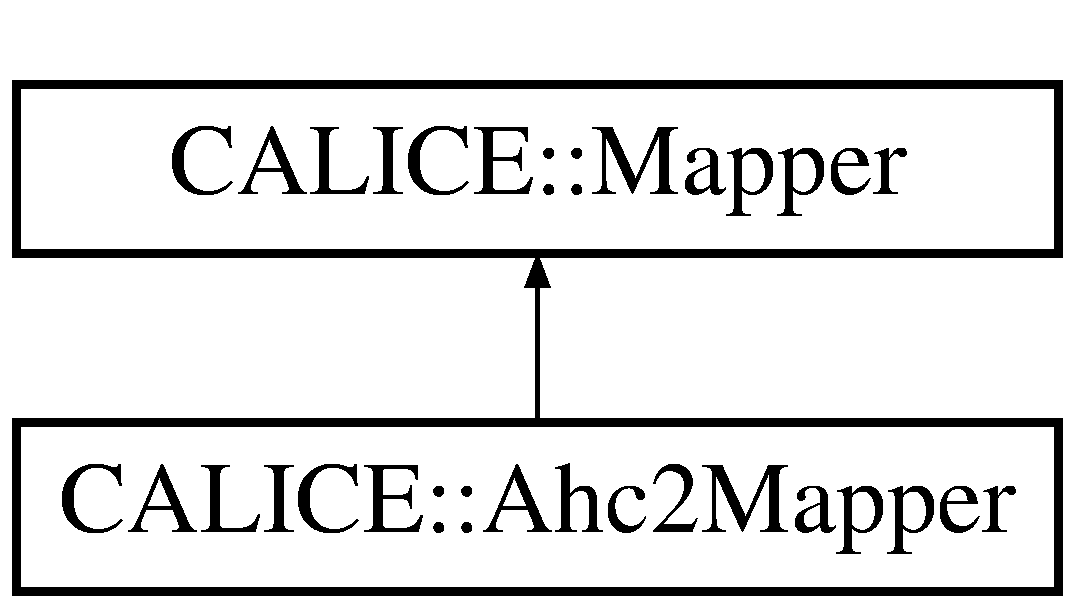
\includegraphics[height=2cm]{classCALICE_1_1Ahc2Mapper}
\end{center}
\end{figure}
\subsection*{Public Member Functions}
\begin{DoxyCompactItemize}
\item 
int {\bf getCellIDFromModChipChan} (const unsigned int module, const unsigned int chip, const unsigned int channel) const 
\begin{DoxyCompactList}\small\item\em generate (Mokka) cellID from module, chip, channel \item\end{DoxyCompactList}\item 
unsigned int {\bf getModuleFromCellID} (const int cellID) const 
\begin{DoxyCompactList}\small\item\em module number from (Mokka) CellID \item\end{DoxyCompactList}\item 
unsigned int {\bf getModuleFromDAQID} (const int DAQchannel) const 
\begin{DoxyCompactList}\small\item\em module number from DAQ channel ID \item\end{DoxyCompactList}\item 
unsigned int {\bf getModule} (const unsigned int crate, const unsigned int slot, const unsigned int fe) const 
\begin{DoxyCompactList}\small\item\em module number from triple crate, slot, fe \item\end{DoxyCompactList}\item 
unsigned int {\bf getModule} (const unsigned int k) const 
\begin{DoxyCompactList}\small\item\em module number from K \item\end{DoxyCompactList}\item 
unsigned int {\bf getModuleFromCellID} (const int cellID, bool \&valid) const 
\begin{DoxyCompactList}\small\item\em get module (number) in which this cell is included from (Mokka) cellID \item\end{DoxyCompactList}\item 
unsigned int {\bf getModuleFromDAQID} (const int DAQchannel, bool \&valid) const 
\begin{DoxyCompactList}\small\item\em get module (number) in which this (DAQ) channel is included \item\end{DoxyCompactList}\item 
unsigned int {\bf getModuleFromModuleID} (const int moduleID, bool \&valid) const 
\begin{DoxyCompactList}\small\item\em get module (number) from this (module) channel ID \item\end{DoxyCompactList}\item 
unsigned int {\bf getChipFromCellID} (const int cellID) const 
\begin{DoxyCompactList}\small\item\em chip number from (Mokka) CellID \item\end{DoxyCompactList}\item 
unsigned int {\bf getChip} (const unsigned int i, const unsigned int j, const unsigned int k) const 
\begin{DoxyCompactList}\small\item\em chip number from triple I, J, K \item\end{DoxyCompactList}\item 
unsigned int {\bf getChanFromCellID} (const int cellID) const 
\begin{DoxyCompactList}\small\item\em channel number from (Mokka) CellID \item\end{DoxyCompactList}\item 
unsigned int {\bf getChan} (const unsigned int i, const unsigned int j, const unsigned int k) const 
\begin{DoxyCompactList}\small\item\em chip number from triple I, J, K \item\end{DoxyCompactList}\item 
unsigned int {\bf getCrateFromCellID} (const int cellID) const 
\begin{DoxyCompactList}\small\item\em crate number from (Mokka) CellID \item\end{DoxyCompactList}\item 
unsigned int {\bf getCrateFromModuleID} (const int moduleID) const 
\begin{DoxyCompactList}\small\item\em crate number from Module cell ID \item\end{DoxyCompactList}\item 
unsigned int {\bf getCrate} (const unsigned int module) const 
\begin{DoxyCompactList}\small\item\em crate number from module number \item\end{DoxyCompactList}\item 
unsigned int {\bf getSlotFromCellID} (const int cellID) const 
\begin{DoxyCompactList}\small\item\em slot number from (Mokka) CellID \item\end{DoxyCompactList}\item 
unsigned int {\bf getSlotFromModuleID} (const int moduleID) const 
\begin{DoxyCompactList}\small\item\em slot number from Module cell ID \item\end{DoxyCompactList}\item 
unsigned int {\bf getSlot} (const unsigned int module) const 
\begin{DoxyCompactList}\small\item\em slot number from module number \item\end{DoxyCompactList}\item 
unsigned int {\bf getFeFromCellID} (const int cellID) const 
\begin{DoxyCompactList}\small\item\em front end number from (Mokka) CellID \item\end{DoxyCompactList}\item 
unsigned int {\bf getFeFromModuleID} (const int moduleID) const 
\begin{DoxyCompactList}\small\item\em front end number from Module cell ID \item\end{DoxyCompactList}\item 
unsigned int {\bf getFe} (const unsigned int module) const 
\begin{DoxyCompactList}\small\item\em front end number from module number \item\end{DoxyCompactList}\item 
unsigned int {\bf getIFromModuleID} (const int moduleID) const 
\begin{DoxyCompactList}\small\item\em I of (Mokka) cellID. \item\end{DoxyCompactList}\item 
unsigned int {\bf getIFromDAQID} (const int DAQchannel) const 
\begin{DoxyCompactList}\small\item\em I of (Mokka) cellID. \item\end{DoxyCompactList}\item 
unsigned int {\bf getI} (const unsigned int module, const unsigned int chip, const unsigned int chan) const 
\begin{DoxyCompactList}\small\item\em I of (Mokka) cellID. \item\end{DoxyCompactList}\item 
unsigned int {\bf getJFromModuleID} (const int moduleID) const 
\begin{DoxyCompactList}\small\item\em J of (Mokka) cellID. \item\end{DoxyCompactList}\item 
unsigned int {\bf getJFromDAQID} (const int DAQchannel) const 
\begin{DoxyCompactList}\small\item\em J of (Mokka) cellID. \item\end{DoxyCompactList}\item 
unsigned int {\bf getJ} (const unsigned int module, const unsigned chip, const unsigned chan) const 
\begin{DoxyCompactList}\small\item\em J of (Mokka) cellID. \item\end{DoxyCompactList}\item 
unsigned int {\bf getKFromModuleID} (const int moduleID) const 
\begin{DoxyCompactList}\small\item\em K of (Mokka) cellID. \item\end{DoxyCompactList}\item 
unsigned int {\bf getKFromDAQID} (const int DAQchannel) const 
\begin{DoxyCompactList}\small\item\em K of (Mokka) cellID. \item\end{DoxyCompactList}\item 
unsigned int {\bf getK} (const unsigned int module) const 
\begin{DoxyCompactList}\small\item\em K of (Mokka) cellID. \item\end{DoxyCompactList}\item 
unsigned int {\bf getISizeFromCellID} (const int cellID) const 
\begin{DoxyCompactList}\small\item\em get cell size in I direction of (Mokka) CellID coordinate \item\end{DoxyCompactList}\item 
unsigned int {\bf getISizeFromModuleID} (const int moduleID) const 
\begin{DoxyCompactList}\small\item\em get cell size in I direction of (Mokka) CellID coordinate \item\end{DoxyCompactList}\item 
unsigned int {\bf getISizeFromDAQID} (const int DAQchannel) const 
\begin{DoxyCompactList}\small\item\em get cell size in I direction of (Mokka) CellID coordinate \item\end{DoxyCompactList}\item 
unsigned int {\bf getISizeFromIJK} (const unsigned int i, const unsigned int j, const unsigned int k) const 
\begin{DoxyCompactList}\small\item\em get cell size in I direction of (Mokka) CellID coordinate \item\end{DoxyCompactList}\item 
unsigned int {\bf getISize} (const unsigned int module, const unsigned int chip, const unsigned int chan) const 
\begin{DoxyCompactList}\small\item\em get cell size in I direction of (Mokka) CellID coordinate \item\end{DoxyCompactList}\item 
unsigned int {\bf getJSizeFromCellID} (const int cellID) const 
\begin{DoxyCompactList}\small\item\em get cell size in J direction of (Mokka) CellID coordinate \item\end{DoxyCompactList}\item 
unsigned int {\bf getJSizeFromModuleID} (const int moduleID) const 
\begin{DoxyCompactList}\small\item\em get cell size in J direction of (Mokka) CellID coordinate \item\end{DoxyCompactList}\item 
unsigned int {\bf getJSizeFromDAQID} (const int DAQchannel) const 
\begin{DoxyCompactList}\small\item\em get cell size in J direction of (Mokka) CellID coordinate \item\end{DoxyCompactList}\item 
unsigned int {\bf getJSizeFromIJK} (const unsigned int i, const unsigned int j, const unsigned int k) const 
\begin{DoxyCompactList}\small\item\em get cell size in J direction of (Mokka) CellID coordinate \item\end{DoxyCompactList}\item 
unsigned int {\bf getJSize} (const unsigned int module, const unsigned int chip, const unsigned int chan) const 
\begin{DoxyCompactList}\small\item\em get cell size in J direction of (Mokka) CellID coordinate \item\end{DoxyCompactList}\item 
int {\bf getTrueCellID} (const int virtualCellIndex) const 
\begin{DoxyCompactList}\small\item\em return identifying index of cell \item\end{DoxyCompactList}\item 
int {\bf getTrueCellID} (const unsigned int i, const unsigned int j, const unsigned int k) const 
\begin{DoxyCompactList}\small\item\em return identifying index of cell \item\end{DoxyCompactList}\item 
unsigned int {\bf getTrueIFromCellID} (const int virtualCellID) const 
\begin{DoxyCompactList}\small\item\em return I of identifying index of cell \item\end{DoxyCompactList}\item 
unsigned int {\bf getTrueIFromIJK} (const unsigned int i, const unsigned int j, const unsigned int k) const 
\begin{DoxyCompactList}\small\item\em return I of identifying index of cell \item\end{DoxyCompactList}\item 
unsigned int {\bf getTrueI} (const unsigned int module, const unsigned int i, const unsigned int j) const 
\begin{DoxyCompactList}\small\item\em return I of identifying index of cell \item\end{DoxyCompactList}\item 
unsigned int {\bf getTrueJFromCellID} (const int virtualCellID) const 
\begin{DoxyCompactList}\small\item\em return J of identifying index of cell \item\end{DoxyCompactList}\item 
unsigned int {\bf getTrueJFromIJK} (const unsigned int i, const unsigned int j, const unsigned int k) const 
\begin{DoxyCompactList}\small\item\em return J of identifying index of cell \item\end{DoxyCompactList}\item 
unsigned int {\bf getTrueJ} (const unsigned int module, const unsigned int i, const unsigned int j) const 
\begin{DoxyCompactList}\small\item\em return J of identifying index of cell \item\end{DoxyCompactList}\item 
unsigned int {\bf getMaxModule} () const 
\begin{DoxyCompactList}\small\item\em return maximum module number \item\end{DoxyCompactList}\item 
unsigned int {\bf getMaxChip} () const 
\begin{DoxyCompactList}\small\item\em return maximum chip number \item\end{DoxyCompactList}\item 
unsigned int {\bf getMaxChannel} () const 
\begin{DoxyCompactList}\small\item\em return maximum channel number \item\end{DoxyCompactList}\item 
unsigned int {\bf getMaxI} () const 
\begin{DoxyCompactList}\small\item\em return maximum I index \item\end{DoxyCompactList}\item 
unsigned int {\bf getMaxJ} () const 
\begin{DoxyCompactList}\small\item\em return maximum J index \item\end{DoxyCompactList}\item 
unsigned int {\bf getMaxK} () const 
\begin{DoxyCompactList}\small\item\em return maximum K index \item\end{DoxyCompactList}\item 
void {\bf fill} (const lcio::LCCollection $\ast$moduleDescriptionCol, const lcio::LCCollection $\ast$moduleConnectionCol)
\begin{DoxyCompactList}\small\item\em fills all necessary mapping information \item\end{DoxyCompactList}\item 
void {\bf updateConnections} (const lcio::LCCollection $\ast$moduleConnectionCol)
\begin{DoxyCompactList}\small\item\em updates the mapping information in the class (possible after first fill only) \item\end{DoxyCompactList}\item 
void {\bf print} (std::ostream \&ostream) const 
\begin{DoxyCompactList}\small\item\em print current data contents \item\end{DoxyCompactList}\item 
void {\bf printStats} (std::ostream \&ostream) const 
\begin{DoxyCompactList}\small\item\em print summary of current data contents \item\end{DoxyCompactList}\end{DoxyCompactItemize}
\subsection*{Protected Member Functions}
\begin{DoxyCompactItemize}
\item 
unsigned int {\bf getIndexByCellID} (const int cellID) const 
\begin{DoxyCompactList}\small\item\em get a compact index for storing data in vectors \item\end{DoxyCompactList}\item 
unsigned int {\bf getIndexByDAQID} (const int ID) const 
\begin{DoxyCompactList}\small\item\em get a compact index for storing data in vectors \item\end{DoxyCompactList}\item 
unsigned int {\bf getIndexByModuleID} (const int ID) const 
\begin{DoxyCompactList}\small\item\em get a compact index for storing data in vectors \item\end{DoxyCompactList}\item 
unsigned int {\bf getMaxIndex} () const 
\begin{DoxyCompactList}\small\item\em get the maximum value of the compact index for storing data in vectors \item\end{DoxyCompactList}\item 
int {\bf getCellIDOfIndex} (unsigned int index) const 
\begin{DoxyCompactList}\small\item\em get the cell ID of a certain compact index \item\end{DoxyCompactList}\end{DoxyCompactItemize}
\subsection*{Private Types}
\begin{DoxyCompactItemize}
\item 
typedef std::map$<$ unsigned int, unsigned int $>$ {\bfseries indexMap\_\-t}\label{classCALICE_1_1Ahc2Mapper_a8fa8a41634f1e55f647a1e4ccb187241}

\end{DoxyCompactItemize}
\subsection*{Private Member Functions}
\begin{DoxyCompactItemize}
\item 
bool {\bfseries valid} (const unsigned int index, const std::vector$<$ bool $>$ \&availableVec) const \label{classCALICE_1_1Ahc2Mapper_a5779fb1d18bd6941001422b70172c479}

\item 
bool {\bfseries valid} (const unsigned int index, const indexMap\_\-t \&indexMap) const \label{classCALICE_1_1Ahc2Mapper_a5ec129a4b5eb89571fac8f991e920c75}

\item 
unsigned int {\bfseries getModuleTypeIndex} (const unsigned int module) const \label{classCALICE_1_1Ahc2Mapper_a7ec97081a91af002c0619e18d4508d0e}

\item 
unsigned int {\bfseries getIndexModuleConnection} (const unsigned int crate, const unsigned int slot, const unsigned int fe) const \label{classCALICE_1_1Ahc2Mapper_a37ed156f74c66d9e2339af8a4deb75d2}

\item 
unsigned int {\bfseries getCrateFromModuleConnectionIndex} (const unsigned int index) const \label{classCALICE_1_1Ahc2Mapper_a6a2c1f1d27a46594fa97f38360feb671}

\item 
unsigned int {\bfseries getSlotFromModuleConnectionIndex} (const unsigned int index) const \label{classCALICE_1_1Ahc2Mapper_abffdd8c1ca5dec03681485a3e2eeab0f}

\item 
unsigned int {\bfseries getFeFromModuleConnectionIndex} (const unsigned int index) const \label{classCALICE_1_1Ahc2Mapper_aeb00ed3940d028aa4ddb3a0758ca24e9}

\item 
unsigned int {\bfseries getCompactIndex} (const unsigned int module, const unsigned int chip, const unsigned int chan) const \label{classCALICE_1_1Ahc2Mapper_aed4b0468a0b060f49c68c5367ecd413a}

\item 
unsigned int {\bfseries getCompactIndex} (const unsigned int module, const unsigned int chanIndex) const \label{classCALICE_1_1Ahc2Mapper_a9c60175d4812ec36d5081c4d2d312b21}

\item 
unsigned int {\bfseries getModuleFromCompactIndex} (const unsigned int index) const \label{classCALICE_1_1Ahc2Mapper_a1a4fbd3f35e9b55f42245da70868f97f}

\item 
unsigned int {\bfseries getChipFromCompactIndex} (const unsigned int index) const \label{classCALICE_1_1Ahc2Mapper_a60e7057cb5a5920ade2cf524798889c7}

\item 
unsigned int {\bfseries getChanFromCompactIndex} (const unsigned int index) const \label{classCALICE_1_1Ahc2Mapper_a2b6d7259a99f3d9b01180ca7954f824d}

\item 
unsigned int {\bfseries getModuleFromIndex} (const unsigned int index, bool \&valid) const \label{classCALICE_1_1Ahc2Mapper_ace765f2bcabc77635c0dfc6f0ccfadf3}

\item 
unsigned int {\bfseries getIndexChan} (const unsigned int chip, const unsigned int chan) const \label{classCALICE_1_1Ahc2Mapper_aa4a115917ac81d3f5035e333587497c8}

\item 
unsigned int {\bfseries getChipFromChanIndex} (const unsigned int index) const \label{classCALICE_1_1Ahc2Mapper_a32ad181b781e10c534bb6bc58b462408}

\item 
unsigned int {\bfseries getChanFromChanIndex} (const unsigned int index) const \label{classCALICE_1_1Ahc2Mapper_a1ccc952c8b8e56d59a91782845cf9002}

\item 
unsigned int {\bfseries getIndexIJ} (const unsigned int i, const unsigned int j) const \label{classCALICE_1_1Ahc2Mapper_acf9ff33c6aa73b1e7d423064dbf47200}

\item 
unsigned int {\bfseries getIFromIJIndex} (const unsigned int index) const \label{classCALICE_1_1Ahc2Mapper_a0afed8a479def3e27f9277647f8fc3a0}

\item 
unsigned int {\bfseries getJFromIJIndex} (const unsigned int index) const \label{classCALICE_1_1Ahc2Mapper_a7f0ca41dc38ec81d8772fbf32c276164}

\item 
void {\bfseries clearCrate} ()\label{classCALICE_1_1Ahc2Mapper_a0dda73f3d42bed14be0bb9a0ea80b9f0}

\item 
void {\bfseries clearSlot} ()\label{classCALICE_1_1Ahc2Mapper_a2edaf45359d58bc56ac4dec0184c8207}

\item 
void {\bfseries clearModuleType} ()\label{classCALICE_1_1Ahc2Mapper_a313a204a51d33156ed7c07cc94eae746}

\item 
{\footnotesize template$<$class T $>$ }\\void {\bfseries initToSize} (std::vector$<$ T $>$ \&vec, const unsigned int size, const T initValue)\label{classCALICE_1_1Ahc2Mapper_a938e92f28a29d7a6e76c3c3b0c3e4da1}

\item 
void {\bfseries initToSize} (std::vector$<$ bool $>$ \&vec, const unsigned int size)\label{classCALICE_1_1Ahc2Mapper_a79a2bcd1def96a4108ef9df7fad2fce3}

\item 
void {\bfseries initToSize} (std::vector$<$ unsigned int $>$ \&dataVec, std::vector$<$ bool $>$ \&availableVec, const unsigned int size)\label{classCALICE_1_1Ahc2Mapper_a6d251a4da1b1132649bcb66d07e8b11d}

\item 
void {\bfseries initFe} (const unsigned int maxFe=0)\label{classCALICE_1_1Ahc2Mapper_a58cf44c88b4ec56fed43d7bfec376051}

\item 
void {\bfseries initModule} (const unsigned int maxMod=0)\label{classCALICE_1_1Ahc2Mapper_a2e16109eb2c7730176d24534f383f097}

\item 
void {\bfseries initK} (const unsigned int maxK=0)\label{classCALICE_1_1Ahc2Mapper_a4ec9ada4c15e3f01168dba3d0fd6c5eb}

\item 
void {\bfseries initIJChipChannel} (const unsigned int maxI=0, const unsigned int maxJ=0, const unsigned int maxChip=0, const unsigned int maxChan=0)\label{classCALICE_1_1Ahc2Mapper_aefb4e5f8d40b42f700b660a5a7107c70}

\item 
void {\bfseries clear} ()\label{classCALICE_1_1Ahc2Mapper_a1b0220e482aa59da0a2cf4024e94af47}

\item 
void {\bfseries registerCrate} (const unsigned int crate)\label{classCALICE_1_1Ahc2Mapper_afe1d35db8e01e9b468c1c99447324239}

\item 
bool {\bfseries crateAvailable} (const unsigned int crate) const \label{classCALICE_1_1Ahc2Mapper_a8e5e8e440475134ba0c57d27f2297444}

\item 
void {\bfseries registerSlot} (const unsigned int slot)\label{classCALICE_1_1Ahc2Mapper_a3fb5cfe4d8fa3344af19490d8023c4d7}

\item 
bool {\bfseries slotAvailable} (const unsigned int slot) const \label{classCALICE_1_1Ahc2Mapper_a31f0e0e105fe686d5f8e0ee26f84aaa4}

\item 
void {\bfseries registerModuleType} (const unsigned int moduleTypeName)\label{classCALICE_1_1Ahc2Mapper_a27be6b81ee87fc5fca72229f6166e625}

\item 
bool {\bfseries moduleTypeAvailable} (const unsigned int moduleTypeName) const \label{classCALICE_1_1Ahc2Mapper_ae730f5461710d7c35dbe78e82624dd5f}

\item 
unsigned int {\bfseries countAvailable} (const std::vector$<$ bool $>$ \&vec) const \label{classCALICE_1_1Ahc2Mapper_a82bfdf21dd843f02ea5be78a049a9007}

\item 
void {\bfseries setModuleCrateSlotFe} (const unsigned int module, const unsigned int crate, const unsigned int slot, const unsigned int fe)\label{classCALICE_1_1Ahc2Mapper_a8bc794db76e3c327e2e41200545792af}

\item 
void {\bfseries setModuleType} (const unsigned int module, const unsigned int typeName)\label{classCALICE_1_1Ahc2Mapper_ad704f5baff47dbdbf1dd06fd6925ec55}

\item 
void {\bfseries setModuleK} (const unsigned int module, const unsigned int K)\label{classCALICE_1_1Ahc2Mapper_a816a00ce81fdd50034fbc72d09369bfb}

\item 
void {\bfseries setModuleTypeIJChipChannel} (const unsigned int moduleTypeName, const unsigned int I, const unsigned int J, const unsigned int sizeI, const unsigned int sizeJ, const unsigned int chip, const unsigned int channel)\label{classCALICE_1_1Ahc2Mapper_a7a07350fa9dd31920670adb2a3c8bdbb}

\item 
void {\bf fillModuleConnection} (const lcio::LCCollection $\ast$col)
\begin{DoxyCompactList}\small\item\em sets the mapping information in the class, call after fillModuleDescription \item\end{DoxyCompactList}\item 
void {\bf fillModuleDescription} (const lcio::LCCollection $\ast$col)
\begin{DoxyCompactList}\small\item\em sets the module layout information in the class, module connection information will be invalidated \item\end{DoxyCompactList}\item 
void {\bfseries getChipChannelForModuleDescriptionID} (const unsigned int id, const unsigned int moduleType, int \&I, int \&J) const \label{classCALICE_1_1Ahc2Mapper_a1bf9c089f6257c21f4272a00c3f65b71}

\item 
unsigned int {\bfseries getCombinedModuleType} (const unsigned int moduleType) const \label{classCALICE_1_1Ahc2Mapper_ab9e334091b3dd2181be96b100af757e8}

\item 
int {\bfseries correctCellIndex} (const unsigned int moduleType, const int cellIndex) const \label{classCALICE_1_1Ahc2Mapper_a78870e67ecf420619165292b00771753}

\item 
const std::string {\bfseries printIfAvailable} (bool available, unsigned int value) const \label{classCALICE_1_1Ahc2Mapper_aa75249c8c6fd4c48a76f41d3022957f7}

\end{DoxyCompactItemize}
\subsection*{Private Attributes}
\begin{DoxyCompactItemize}
\item 
unsigned int {\bfseries \_\-nChan}\label{classCALICE_1_1Ahc2Mapper_a9fa2e4f1e3a71c11e358f1dc51cc5fd5}

\item 
unsigned int {\bfseries \_\-nChip}\label{classCALICE_1_1Ahc2Mapper_a0e529c3d73a93f42e26319eef4b33d44}

\item 
unsigned int {\bfseries \_\-nFe}\label{classCALICE_1_1Ahc2Mapper_a1686f7a7a65fdca2a348587b5ab9600d}

\item 
unsigned int {\bfseries \_\-nSlot}\label{classCALICE_1_1Ahc2Mapper_a40593547c68870acc499e76687cfb883}

\item 
unsigned int {\bfseries \_\-maxSlot}\label{classCALICE_1_1Ahc2Mapper_aa58dcfea6768a674f86295b0479a7ea1}

\item 
unsigned int {\bfseries \_\-nCrate}\label{classCALICE_1_1Ahc2Mapper_a0409a71622d7feb7af789d1bed2bf502}

\item 
unsigned int {\bfseries \_\-nMod}\label{classCALICE_1_1Ahc2Mapper_a30959038e7a47577fe830d02f5c42030}

\item 
unsigned int {\bfseries \_\-nModType}\label{classCALICE_1_1Ahc2Mapper_a78504bc4de22b3408b8a00f705b3a866}

\item 
unsigned int {\bfseries \_\-nI}\label{classCALICE_1_1Ahc2Mapper_a6844cfc402304fc896308969b7028746}

\item 
unsigned int {\bfseries \_\-nJ}\label{classCALICE_1_1Ahc2Mapper_a38b7139f1417342711f1521855cc5c06}

\item 
unsigned int {\bfseries \_\-nK}\label{classCALICE_1_1Ahc2Mapper_a6835d7c3ee234599a41f6c92c221d782}

\item 
indexMap\_\-t {\bfseries \_\-crateIndex}\label{classCALICE_1_1Ahc2Mapper_a72f2d3b1123afe37a965760553af31df}

\item 
std::vector$<$ unsigned int $>$ {\bfseries \_\-crateNumber}\label{classCALICE_1_1Ahc2Mapper_a99f99ee105d7a92cad6a1b2de137051c}

\item 
std::vector$<$ unsigned int $>$ {\bfseries \_\-slotIndex}\label{classCALICE_1_1Ahc2Mapper_abed822b374b582b73ba5eb1a1a72650e}

\item 
std::vector$<$ unsigned int $>$ {\bfseries \_\-slotNumber}\label{classCALICE_1_1Ahc2Mapper_a09a25b93e65b8050686fbeb1a4bf4fe5}

\item 
std::vector$<$ bool $>$ {\bfseries \_\-slotAvailable}\label{classCALICE_1_1Ahc2Mapper_a2c726b690ab826d55b453818c52eb3ff}

\item 
std::vector$<$ bool $>$ {\bfseries \_\-connectionAvailable}\label{classCALICE_1_1Ahc2Mapper_aa6c87b52cea16672077a07b6792b0971}

\item 
std::vector$<$ bool $>$ {\bfseries \_\-moduleAvailable}\label{classCALICE_1_1Ahc2Mapper_a95bdac10e6000d097c537719e24545ac}

\item 
std::vector$<$ unsigned int $>$ {\bfseries \_\-typeVmodule}\label{classCALICE_1_1Ahc2Mapper_a0580a43e47c99b8db25aaa5a9ac8cc5a}

\item 
std::vector$<$ unsigned int $>$ {\bfseries \_\-connectionVmodule}\label{classCALICE_1_1Ahc2Mapper_a2e2b5d4ee46b39d39cb5fa6cde1146b6}

\item 
std::vector$<$ bool $>$ {\bfseries \_\-connectionVmoduleAvailable}\label{classCALICE_1_1Ahc2Mapper_a83a1e56f89237e258c3a31099f8bdbbf}

\item 
std::vector$<$ unsigned int $>$ {\bfseries \_\-moduleVconnection}\label{classCALICE_1_1Ahc2Mapper_aedbaa5da8322fd4eccaac3fb83882766}

\item 
std::vector$<$ unsigned int $>$ {\bfseries \_\-kVmodule}\label{classCALICE_1_1Ahc2Mapper_aab6dabe051d9b636830b7acba209d93e}

\item 
std::vector$<$ bool $>$ {\bfseries \_\-kVmoduleAvailable}\label{classCALICE_1_1Ahc2Mapper_acf9257d540b74e5ca84312e34a6c2813}

\item 
std::vector$<$ unsigned int $>$ {\bfseries \_\-moduleVk}\label{classCALICE_1_1Ahc2Mapper_ad9d8d380bce5a616ed41e27de9d0fda4}

\item 
std::vector$<$ bool $>$ {\bfseries \_\-kAvailable}\label{classCALICE_1_1Ahc2Mapper_ae2e9161b57b9d271884aa1fdfb0299bc}

\item 
std::vector$<$ unsigned int $>$ {\bfseries \_\-moduleTypeName}\label{classCALICE_1_1Ahc2Mapper_a6d569495b69bb4d9dac977bb26df6135}

\item 
std::vector$<$ unsigned int $>$ {\bfseries \_\-moduleTypeIndex}\label{classCALICE_1_1Ahc2Mapper_a9861340fda5c1149dc6fbabb5132865a}

\item 
std::vector$<$ bool $>$ {\bfseries \_\-moduleTypeAvailable}\label{classCALICE_1_1Ahc2Mapper_a93e90fa76f22daabcb65e598e5bfed51}

\item 
std::vector$<$ std::vector$<$ unsigned int $>$ $>$ {\bfseries \_\-ijVchan}\label{classCALICE_1_1Ahc2Mapper_a7e7cfcfc84871aab429cae7ceb83977d}

\item 
std::vector$<$ std::vector$<$ bool $>$ $>$ {\bfseries \_\-chipChanAvailable}\label{classCALICE_1_1Ahc2Mapper_a338e6d91a30e082dd6c9887b595bbc73}

\item 
std::vector$<$ std::vector$<$ unsigned int $>$ $>$ {\bfseries \_\-chanVij}\label{classCALICE_1_1Ahc2Mapper_ae93966f8bbc2d7f2681c1e8165b81240}

\item 
std::vector$<$ std::vector$<$ bool $>$ $>$ {\bfseries \_\-ijAvailable}\label{classCALICE_1_1Ahc2Mapper_acc072178aa9b3396f9abc4e60296d6c5}

\item 
std::vector$<$ std::vector$<$ bool $>$ $>$ {\bfseries \_\-ijSecondaryAvailable}\label{classCALICE_1_1Ahc2Mapper_a23243017bd70e95e3788828c408cfa78}

\item 
std::vector$<$ std::vector$<$ unsigned int $>$ $>$ {\bfseries \_\-sizeIVchan}\label{classCALICE_1_1Ahc2Mapper_ad1e47929482e3c583cd726da48bcdb68}

\item 
std::vector$<$ std::vector$<$ unsigned int $>$ $>$ {\bfseries \_\-sizeJVchan}\label{classCALICE_1_1Ahc2Mapper_adfab042b239b997051a6c11409dab982}

\end{DoxyCompactItemize}


\subsection{Detailed Description}
AHCAL implementation of \doxyref{Mapper}{p.}{classCALICE_1_1Mapper} class. \begin{DoxyParagraph}{invalid cells and exception handling}
Most functions throw a \doxyref{CALICE::BadDataException}{p.}{classCALICE_1_1BadDataException} if an invalid combination or ID is queried. Not all invalid combinations will be detected by all commands, depending on the necessary coordinate transformations in the command. E.g.: When querying the module from a Mokka cell ID, only K is extracted from the ID. If no module exists for this K an exception is thrown. But there will be no exception thrown if K is valid but I and J belong to a channel which does not exist in this module.
\end{DoxyParagraph}
\begin{DoxyParagraph}{}
The protected getIndexFunctions do {\bfseries not} throw exceptions to allow a fast lookup of the index. Invalid channels are signalled with return value maxIndex+1.
\end{DoxyParagraph}
\begin{DoxyParagraph}{}
Some functions have a second version that does a full check if the ID is valid without throwing an exception.
\end{DoxyParagraph}
\begin{DoxyAuthor}{Author}
{\tt Shaojun.lu@desy.de} 
\end{DoxyAuthor}
\begin{DoxyVersion}{Version}
0.1 
\end{DoxyVersion}
\begin{DoxyDate}{Date}
May 2013 
\end{DoxyDate}


Definition at line 44 of file Ahc2Mapper.hh.

\subsection{Member Function Documentation}
\index{CALICE::Ahc2Mapper@{CALICE::Ahc2Mapper}!fill@{fill}}
\index{fill@{fill}!CALICE::Ahc2Mapper@{CALICE::Ahc2Mapper}}
\subsubsection[{fill}]{\setlength{\rightskip}{0pt plus 5cm}void CALICE::Ahc2Mapper::fill (const lcio::LCCollection $\ast$ {\em moduleDescriptionCol}, \/  const lcio::LCCollection $\ast$ {\em moduleConnectionCol})\hspace{0.3cm}{\ttfamily  [inline]}}\label{classCALICE_1_1Ahc2Mapper_a2665c4a607dec1613e91e89bb652195e}


fills all necessary mapping information Module layout types are set from moduleDescription (chip,channel to I,J,K \& size) Module connections are set from moduleConnection (crate, slot, fe to module)

Old settings are cleared before new are set.


\begin{DoxyParams}{Parameters}
\item[\mbox{$\leftarrow$} {\em moduleDescriptionCol}]LCGenericObject collection of \doxyref{ModuleDescription}{p.}{classCALICE_1_1ModuleDescription} type \item[\mbox{$\leftarrow$} {\em moduleConnectionCol}]LCGenericObject collection of \doxyref{ModuleConnection}{p.}{classCALICE_1_1ModuleConnection} type \end{DoxyParams}


Definition at line 946 of file Ahc2Mapper.hh.

References fillModuleConnection(), and fillModuleDescription().\index{CALICE::Ahc2Mapper@{CALICE::Ahc2Mapper}!fillModuleConnection@{fillModuleConnection}}
\index{fillModuleConnection@{fillModuleConnection}!CALICE::Ahc2Mapper@{CALICE::Ahc2Mapper}}
\subsubsection[{fillModuleConnection}]{\setlength{\rightskip}{0pt plus 5cm}void CALICE::Ahc2Mapper::fillModuleConnection (const lcio::LCCollection $\ast$ {\em col})\hspace{0.3cm}{\ttfamily  [private]}}\label{classCALICE_1_1Ahc2Mapper_a24e7b07d1fbac2bc225a1af08fa52d38}


sets the mapping information in the class, call after fillModuleDescription The internal mapping of modules to type and electronics connection is set.


\begin{DoxyParams}{Parameters}
\item[\mbox{$\leftarrow$} {\em col}]LCGenericObject collection of \doxyref{ModuleConnection}{p.}{classCALICE_1_1ModuleConnection} type \end{DoxyParams}


Definition at line 15 of file Ahc2Mapper.cc.

References CALICE::Mapper::mappingModified().

Referenced by fill(), and updateConnections().\index{CALICE::Ahc2Mapper@{CALICE::Ahc2Mapper}!fillModuleDescription@{fillModuleDescription}}
\index{fillModuleDescription@{fillModuleDescription}!CALICE::Ahc2Mapper@{CALICE::Ahc2Mapper}}
\subsubsection[{fillModuleDescription}]{\setlength{\rightskip}{0pt plus 5cm}void CALICE::Ahc2Mapper::fillModuleDescription (const lcio::LCCollection $\ast$ {\em col})\hspace{0.3cm}{\ttfamily  [private]}}\label{classCALICE_1_1Ahc2Mapper_a72a2159c191b2413a13408c2f9c24480}


sets the module layout information in the class, module connection information will be invalidated The internal layout of modules, like channel to I,J,K and cell sizes are set.

\begin{DoxyWarning}{Warning}
module connection information will be invalidated, fillModuleConnection has to be called aftwards
\end{DoxyWarning}

\begin{DoxyParams}{Parameters}
\item[\mbox{$\leftarrow$} {\em col}]LCGenericObject collection of \doxyref{ModuleDescription}{p.}{classCALICE_1_1ModuleDescription} type \end{DoxyParams}


Definition at line 117 of file Ahc2Mapper.cc.

References CALICE::CellIndex::getPadColumn(), CALICE::CellIndex::getPadRow(), and CALICE::Mapper::mappingModified().

Referenced by fill().\index{CALICE::Ahc2Mapper@{CALICE::Ahc2Mapper}!getCellIDOfIndex@{getCellIDOfIndex}}
\index{getCellIDOfIndex@{getCellIDOfIndex}!CALICE::Ahc2Mapper@{CALICE::Ahc2Mapper}}
\subsubsection[{getCellIDOfIndex}]{\setlength{\rightskip}{0pt plus 5cm}int CALICE::Ahc2Mapper::getCellIDOfIndex (unsigned int {\em index}) const\hspace{0.3cm}{\ttfamily  [inline, protected, virtual]}}\label{classCALICE_1_1Ahc2Mapper_aa622a971f22c254c324a817355257bdc}


get the cell ID of a certain compact index \begin{DoxyWarning}{Warning}
This cell ID will only contain information about I, J and K. If the encoding string contains additional fields this will have value 0.
\end{DoxyWarning}
\begin{DoxySeeAlso}{See also}
setCellIDencoding
\end{DoxySeeAlso}
\begin{DoxyReturn}{Returns}
(Mokka) cell ID 
\end{DoxyReturn}


Implements {\bf CALICE::Mapper} \doxyref{}{p.}{group__CellIDgroup_ga1157f15cfe97ad035e6f6fb2fd32ce2e}.

Definition at line 1070 of file Ahc2Mapper.hh.

References CALICE::DecoderSet::getCellID(), CALICE::Mapper::getDecoder(), getI(), getJ(), and getK().\index{CALICE::Ahc2Mapper@{CALICE::Ahc2Mapper}!getChan@{getChan}}
\index{getChan@{getChan}!CALICE::Ahc2Mapper@{CALICE::Ahc2Mapper}}
\subsubsection[{getChan}]{\setlength{\rightskip}{0pt plus 5cm}unsigned int CALICE::Ahc2Mapper::getChan (const unsigned int {\em i}, \/  const unsigned int {\em j}, \/  const unsigned int {\em k}) const\hspace{0.3cm}{\ttfamily  [inline]}}\label{classCALICE_1_1Ahc2Mapper_a9e2aa9c28a73ef59895d251604c6cfbb}


chip number from triple I, J, K 
\begin{DoxyParams}{Parameters}
\item[\mbox{$\leftarrow$} {\em i}]I \item[\mbox{$\leftarrow$} {\em j}]J \item[\mbox{$\leftarrow$} {\em k}]K\end{DoxyParams}

\begin{DoxyExceptions}{Exceptions}
\item[{\em \doxyref{BadDataException}{p.}{classCALICE_1_1BadDataException}}]if invalid channel\end{DoxyExceptions}
\begin{DoxyReturn}{Returns}
channel number 
\end{DoxyReturn}


Definition at line 264 of file Ahc2Mapper.hh.

References getModule().

Referenced by getChanFromCellID(), getISizeFromIJK(), and getJSizeFromIJK().\index{CALICE::Ahc2Mapper@{CALICE::Ahc2Mapper}!getChip@{getChip}}
\index{getChip@{getChip}!CALICE::Ahc2Mapper@{CALICE::Ahc2Mapper}}
\subsubsection[{getChip}]{\setlength{\rightskip}{0pt plus 5cm}unsigned int CALICE::Ahc2Mapper::getChip (const unsigned int {\em i}, \/  const unsigned int {\em j}, \/  const unsigned int {\em k}) const\hspace{0.3cm}{\ttfamily  [inline]}}\label{classCALICE_1_1Ahc2Mapper_a3b4555ddb636f3a1def55d7e21248b95}


chip number from triple I, J, K 
\begin{DoxyParams}{Parameters}
\item[\mbox{$\leftarrow$} {\em i}]I \item[\mbox{$\leftarrow$} {\em j}]J \item[\mbox{$\leftarrow$} {\em k}]K\end{DoxyParams}

\begin{DoxyExceptions}{Exceptions}
\item[{\em \doxyref{BadDataException}{p.}{classCALICE_1_1BadDataException}}]if lookup fails\end{DoxyExceptions}
\begin{DoxyReturn}{Returns}
chip number 
\end{DoxyReturn}


Definition at line 228 of file Ahc2Mapper.hh.

References getModule().

Referenced by getChipFromCellID(), getISizeFromIJK(), and getJSizeFromIJK().\index{CALICE::Ahc2Mapper@{CALICE::Ahc2Mapper}!getCrate@{getCrate}}
\index{getCrate@{getCrate}!CALICE::Ahc2Mapper@{CALICE::Ahc2Mapper}}
\subsubsection[{getCrate}]{\setlength{\rightskip}{0pt plus 5cm}unsigned int CALICE::Ahc2Mapper::getCrate (const unsigned int {\em module}) const\hspace{0.3cm}{\ttfamily  [inline]}}\label{classCALICE_1_1Ahc2Mapper_a085945b3737a8a6c55a4db7c441e9808}


crate number from module number 
\begin{DoxyParams}{Parameters}
\item[\mbox{$\leftarrow$} {\em module}]module number\end{DoxyParams}

\begin{DoxyExceptions}{Exceptions}
\item[{\em \doxyref{BadDataException}{p.}{classCALICE_1_1BadDataException}}]if lookup fails\end{DoxyExceptions}
\begin{DoxyReturn}{Returns}
crate number 
\end{DoxyReturn}


Definition at line 312 of file Ahc2Mapper.hh.

Referenced by getCrateFromCellID(), getCrateFromModuleID(), and print().\index{CALICE::Ahc2Mapper@{CALICE::Ahc2Mapper}!getFe@{getFe}}
\index{getFe@{getFe}!CALICE::Ahc2Mapper@{CALICE::Ahc2Mapper}}
\subsubsection[{getFe}]{\setlength{\rightskip}{0pt plus 5cm}unsigned int CALICE::Ahc2Mapper::getFe (const unsigned int {\em module}) const\hspace{0.3cm}{\ttfamily  [inline]}}\label{classCALICE_1_1Ahc2Mapper_aba331d42b7ba82dd24f2ee6843d704c4}


front end number from module number 
\begin{DoxyParams}{Parameters}
\item[\mbox{$\leftarrow$} {\em module}]module number\end{DoxyParams}

\begin{DoxyExceptions}{Exceptions}
\item[{\em \doxyref{BadDataException}{p.}{classCALICE_1_1BadDataException}}]if lookup fails\end{DoxyExceptions}
\begin{DoxyReturn}{Returns}
front end number 
\end{DoxyReturn}


Definition at line 399 of file Ahc2Mapper.hh.

Referenced by getFeFromCellID(), getFeFromModuleID(), and print().\index{CALICE::Ahc2Mapper@{CALICE::Ahc2Mapper}!getI@{getI}}
\index{getI@{getI}!CALICE::Ahc2Mapper@{CALICE::Ahc2Mapper}}
\subsubsection[{getI}]{\setlength{\rightskip}{0pt plus 5cm}unsigned int CALICE::Ahc2Mapper::getI (const unsigned int {\em module}, \/  const unsigned int {\em chip}, \/  const unsigned int {\em chan}) const\hspace{0.3cm}{\ttfamily  [inline]}}\label{classCALICE_1_1Ahc2Mapper_a68be5ca889254e15dc98f8ded619d2d6}


I of (Mokka) cellID. 
\begin{DoxyParams}{Parameters}
\item[\mbox{$\leftarrow$} {\em module}]module number \item[\mbox{$\leftarrow$} {\em chip}]chip number \item[\mbox{$\leftarrow$} {\em chan}]channel number\end{DoxyParams}

\begin{DoxyExceptions}{Exceptions}
\item[{\em \doxyref{BadDataException}{p.}{classCALICE_1_1BadDataException}}]if lookup fails\end{DoxyExceptions}
\begin{DoxyReturn}{Returns}
I 
\end{DoxyReturn}


Definition at line 444 of file Ahc2Mapper.hh.

Referenced by getCellIDFromModChipChan(), getCellIDOfIndex(), getIFromDAQID(), and getIFromModuleID().\index{CALICE::Ahc2Mapper@{CALICE::Ahc2Mapper}!getIndexByCellID@{getIndexByCellID}}
\index{getIndexByCellID@{getIndexByCellID}!CALICE::Ahc2Mapper@{CALICE::Ahc2Mapper}}
\subsubsection[{getIndexByCellID}]{\setlength{\rightskip}{0pt plus 5cm}unsigned int CALICE::Ahc2Mapper::getIndexByCellID (const int {\em cellID}) const\hspace{0.3cm}{\ttfamily  [inline, protected, virtual]}}\label{classCALICE_1_1Ahc2Mapper_aa468f8c91286f9452202e0de9dc86179}


get a compact index for storing data in vectors 
\begin{DoxyParams}{Parameters}
\item[\mbox{$\leftarrow$} {\em cellID}](Mokka) cell ID \end{DoxyParams}
\begin{DoxyReturn}{Returns}
compact index 
\end{DoxyReturn}


Implements {\bf CALICE::Mapper} \doxyref{}{p.}{group__CellIDgroup_gaaa6d826a6990c070c769f9754d2fbb76}.

Definition at line 984 of file Ahc2Mapper.hh.

References CALICE::Mapper::getDecoder(), CALICE::DecoderSet::getIFromCellID(), CALICE::DecoderSet::getJFromCellID(), CALICE::DecoderSet::getKFromCellID(), and getMaxIndex().

Referenced by getModuleFromCellID().\index{CALICE::Ahc2Mapper@{CALICE::Ahc2Mapper}!getIndexByDAQID@{getIndexByDAQID}}
\index{getIndexByDAQID@{getIndexByDAQID}!CALICE::Ahc2Mapper@{CALICE::Ahc2Mapper}}
\subsubsection[{getIndexByDAQID}]{\setlength{\rightskip}{0pt plus 5cm}unsigned int CALICE::Ahc2Mapper::getIndexByDAQID (const int {\em ID}) const\hspace{0.3cm}{\ttfamily  [inline, protected, virtual]}}\label{classCALICE_1_1Ahc2Mapper_a8503c24f6eab43e134845efc48654908}


get a compact index for storing data in vectors 
\begin{DoxyParams}{Parameters}
\item[\mbox{$\leftarrow$} {\em ID}]DAQ channel ID \end{DoxyParams}
\begin{DoxyReturn}{Returns}
compact index 
\end{DoxyReturn}


Implements {\bf CALICE::Mapper} \doxyref{}{p.}{group__DAQgroup_ga4c00b2760cd3e935bed9db2f3fd28b06}.

Definition at line 1007 of file Ahc2Mapper.hh.

References CALICE::DecoderSet::getChannelFromDAQID(), CALICE::DecoderSet::getChipFromDAQID(), CALICE::DecoderSet::getCrateFromDAQID(), CALICE::Mapper::getDecoder(), CALICE::DecoderSet::getFeFromDAQID(), getMaxIndex(), and CALICE::DecoderSet::getSlotFromDAQID().

Referenced by getModuleFromDAQID().\index{CALICE::Ahc2Mapper@{CALICE::Ahc2Mapper}!getIndexByModuleID@{getIndexByModuleID}}
\index{getIndexByModuleID@{getIndexByModuleID}!CALICE::Ahc2Mapper@{CALICE::Ahc2Mapper}}
\subsubsection[{getIndexByModuleID}]{\setlength{\rightskip}{0pt plus 5cm}unsigned int CALICE::Ahc2Mapper::getIndexByModuleID (const int {\em ID}) const\hspace{0.3cm}{\ttfamily  [inline, protected, virtual]}}\label{classCALICE_1_1Ahc2Mapper_a3471e5014da85986b145f08b977d2e94}


get a compact index for storing data in vectors 
\begin{DoxyParams}{Parameters}
\item[\mbox{$\leftarrow$} {\em ID}]Module channel ID \end{DoxyParams}
\begin{DoxyReturn}{Returns}
compact index 
\end{DoxyReturn}


Implements {\bf CALICE::Mapper} \doxyref{}{p.}{group__ModuleIDgroup_gad546fcc374c9168872a957d90d62bda3}.

Definition at line 1042 of file Ahc2Mapper.hh.

References CALICE::DecoderSet::getChannelFromModuleID(), CALICE::DecoderSet::getChipFromModuleID(), CALICE::Mapper::getDecoder(), getMaxIndex(), and CALICE::DecoderSet::getModuleFromModuleID().

Referenced by getModuleFromModuleID().\index{CALICE::Ahc2Mapper@{CALICE::Ahc2Mapper}!getISize@{getISize}}
\index{getISize@{getISize}!CALICE::Ahc2Mapper@{CALICE::Ahc2Mapper}}
\subsubsection[{getISize}]{\setlength{\rightskip}{0pt plus 5cm}unsigned int CALICE::Ahc2Mapper::getISize (const unsigned int {\em module}, \/  const unsigned int {\em chip}, \/  const unsigned int {\em chan}) const\hspace{0.3cm}{\ttfamily  [inline]}}\label{classCALICE_1_1Ahc2Mapper_a52d8a9ca0d55fc87f92d339ec763b514}


get cell size in I direction of (Mokka) CellID coordinate 
\begin{DoxyParams}{Parameters}
\item[\mbox{$\leftarrow$} {\em module}]module number \item[\mbox{$\leftarrow$} {\em chip}]chip number \item[\mbox{$\leftarrow$} {\em chan}]channel number\end{DoxyParams}
\begin{DoxyReturn}{Returns}
size in I
\end{DoxyReturn}

\begin{DoxyExceptions}{Exceptions}
\item[{\em \doxyref{BadDataException}{p.}{classCALICE_1_1BadDataException}}]if lookup fails \end{DoxyExceptions}


Definition at line 614 of file Ahc2Mapper.hh.

Referenced by getISizeFromDAQID(), getISizeFromIJK(), and getISizeFromModuleID().\index{CALICE::Ahc2Mapper@{CALICE::Ahc2Mapper}!getISizeFromIJK@{getISizeFromIJK}}
\index{getISizeFromIJK@{getISizeFromIJK}!CALICE::Ahc2Mapper@{CALICE::Ahc2Mapper}}
\subsubsection[{getISizeFromIJK}]{\setlength{\rightskip}{0pt plus 5cm}unsigned int CALICE::Ahc2Mapper::getISizeFromIJK (const unsigned int {\em i}, \/  const unsigned int {\em j}, \/  const unsigned int {\em k}) const\hspace{0.3cm}{\ttfamily  [inline]}}\label{classCALICE_1_1Ahc2Mapper_acf96a7b43c787c30876d5a3b8df68a5c}


get cell size in I direction of (Mokka) CellID coordinate 
\begin{DoxyParams}{Parameters}
\item[\mbox{$\leftarrow$} {\em i}]I \item[\mbox{$\leftarrow$} {\em j}]J \item[\mbox{$\leftarrow$} {\em k}]K\end{DoxyParams}
\begin{DoxyReturn}{Returns}
size in I
\end{DoxyReturn}

\begin{DoxyExceptions}{Exceptions}
\item[{\em \doxyref{BadDataException}{p.}{classCALICE_1_1BadDataException}}]if lookup fails \end{DoxyExceptions}


Definition at line 600 of file Ahc2Mapper.hh.

References getChan(), getChip(), getISize(), and getModule().

Referenced by getISizeFromCellID().\index{CALICE::Ahc2Mapper@{CALICE::Ahc2Mapper}!getJ@{getJ}}
\index{getJ@{getJ}!CALICE::Ahc2Mapper@{CALICE::Ahc2Mapper}}
\subsubsection[{getJ}]{\setlength{\rightskip}{0pt plus 5cm}unsigned int CALICE::Ahc2Mapper::getJ (const unsigned int {\em module}, \/  const unsigned {\em chip}, \/  const unsigned {\em chan}) const\hspace{0.3cm}{\ttfamily  [inline]}}\label{classCALICE_1_1Ahc2Mapper_a50f1c14d9fb052f9ec91fc7611cf86a9}


J of (Mokka) cellID. 
\begin{DoxyParams}{Parameters}
\item[\mbox{$\leftarrow$} {\em module}]module number \item[\mbox{$\leftarrow$} {\em chip}]chip number \item[\mbox{$\leftarrow$} {\em chan}]channel number\end{DoxyParams}

\begin{DoxyExceptions}{Exceptions}
\item[{\em \doxyref{BadDataException}{p.}{classCALICE_1_1BadDataException}}]if lookup fails\end{DoxyExceptions}
\begin{DoxyReturn}{Returns}
J 
\end{DoxyReturn}


Definition at line 493 of file Ahc2Mapper.hh.

Referenced by getCellIDFromModChipChan(), getCellIDOfIndex(), getJFromDAQID(), and getJFromModuleID().\index{CALICE::Ahc2Mapper@{CALICE::Ahc2Mapper}!getJSize@{getJSize}}
\index{getJSize@{getJSize}!CALICE::Ahc2Mapper@{CALICE::Ahc2Mapper}}
\subsubsection[{getJSize}]{\setlength{\rightskip}{0pt plus 5cm}unsigned int CALICE::Ahc2Mapper::getJSize (const unsigned int {\em module}, \/  const unsigned int {\em chip}, \/  const unsigned int {\em chan}) const\hspace{0.3cm}{\ttfamily  [inline]}}\label{classCALICE_1_1Ahc2Mapper_a2a086e94e80f98fd77ba49656a42f036}


get cell size in J direction of (Mokka) CellID coordinate 
\begin{DoxyParams}{Parameters}
\item[\mbox{$\leftarrow$} {\em module}]module number \item[\mbox{$\leftarrow$} {\em chip}]chip number \item[\mbox{$\leftarrow$} {\em chan}]channel number\end{DoxyParams}
\begin{DoxyReturn}{Returns}
size in J
\end{DoxyReturn}

\begin{DoxyExceptions}{Exceptions}
\item[{\em \doxyref{BadDataException}{p.}{classCALICE_1_1BadDataException}}]if lookup fails \end{DoxyExceptions}


Definition at line 692 of file Ahc2Mapper.hh.

Referenced by getJSizeFromDAQID(), getJSizeFromIJK(), and getJSizeFromModuleID().\index{CALICE::Ahc2Mapper@{CALICE::Ahc2Mapper}!getJSizeFromIJK@{getJSizeFromIJK}}
\index{getJSizeFromIJK@{getJSizeFromIJK}!CALICE::Ahc2Mapper@{CALICE::Ahc2Mapper}}
\subsubsection[{getJSizeFromIJK}]{\setlength{\rightskip}{0pt plus 5cm}unsigned int CALICE::Ahc2Mapper::getJSizeFromIJK (const unsigned int {\em i}, \/  const unsigned int {\em j}, \/  const unsigned int {\em k}) const\hspace{0.3cm}{\ttfamily  [inline]}}\label{classCALICE_1_1Ahc2Mapper_a255332c0e41298be7325bb1a91658abb}


get cell size in J direction of (Mokka) CellID coordinate 
\begin{DoxyParams}{Parameters}
\item[\mbox{$\leftarrow$} {\em i}]I \item[\mbox{$\leftarrow$} {\em j}]J \item[\mbox{$\leftarrow$} {\em k}]K\end{DoxyParams}
\begin{DoxyReturn}{Returns}
size in J
\end{DoxyReturn}

\begin{DoxyExceptions}{Exceptions}
\item[{\em \doxyref{BadDataException}{p.}{classCALICE_1_1BadDataException}}]if lookup fails \end{DoxyExceptions}


Definition at line 678 of file Ahc2Mapper.hh.

References getChan(), getChip(), getJSize(), and getModule().

Referenced by getJSizeFromCellID().\index{CALICE::Ahc2Mapper@{CALICE::Ahc2Mapper}!getK@{getK}}
\index{getK@{getK}!CALICE::Ahc2Mapper@{CALICE::Ahc2Mapper}}
\subsubsection[{getK}]{\setlength{\rightskip}{0pt plus 5cm}unsigned int CALICE::Ahc2Mapper::getK (const unsigned int {\em module}) const\hspace{0.3cm}{\ttfamily  [inline]}}\label{classCALICE_1_1Ahc2Mapper_aa246f415919db6fa4a7139f0907f3856}


K of (Mokka) cellID. 
\begin{DoxyParams}{Parameters}
\item[\mbox{$\leftarrow$} {\em module}]module number\end{DoxyParams}
\begin{DoxyReturn}{Returns}
K
\end{DoxyReturn}

\begin{DoxyExceptions}{Exceptions}
\item[{\em \doxyref{BadDataException}{p.}{classCALICE_1_1BadDataException}}]if lookup fails \end{DoxyExceptions}


Definition at line 540 of file Ahc2Mapper.hh.

Referenced by getCellIDFromModChipChan(), getCellIDOfIndex(), getKFromDAQID(), getKFromModuleID(), and print().\index{CALICE::Ahc2Mapper@{CALICE::Ahc2Mapper}!getMaxIndex@{getMaxIndex}}
\index{getMaxIndex@{getMaxIndex}!CALICE::Ahc2Mapper@{CALICE::Ahc2Mapper}}
\subsubsection[{getMaxIndex}]{\setlength{\rightskip}{0pt plus 5cm}unsigned int CALICE::Ahc2Mapper::getMaxIndex () const\hspace{0.3cm}{\ttfamily  [inline, protected, virtual]}}\label{classCALICE_1_1Ahc2Mapper_a628441b11caa652f1d13599675b8da6d}


get the maximum value of the compact index for storing data in vectors \begin{DoxyReturn}{Returns}
maximum compact index 
\end{DoxyReturn}


Implements {\bf CALICE::Mapper} \doxyref{}{p.}{classCALICE_1_1Mapper_a34292aca2d87f6fc7f10094b5f7cab0e}.

Definition at line 1066 of file Ahc2Mapper.hh.

Referenced by getIndexByCellID(), getIndexByDAQID(), and getIndexByModuleID().\index{CALICE::Ahc2Mapper@{CALICE::Ahc2Mapper}!getModule@{getModule}}
\index{getModule@{getModule}!CALICE::Ahc2Mapper@{CALICE::Ahc2Mapper}}
\subsubsection[{getModule}]{\setlength{\rightskip}{0pt plus 5cm}unsigned int CALICE::Ahc2Mapper::getModule (const unsigned int {\em k}) const\hspace{0.3cm}{\ttfamily  [inline]}}\label{classCALICE_1_1Ahc2Mapper_a43d10d6fa909332e4744fce0986b9bc4}


module number from K 
\begin{DoxyParams}{Parameters}
\item[\mbox{$\leftarrow$} {\em k}]K\end{DoxyParams}

\begin{DoxyExceptions}{Exceptions}
\item[{\em \doxyref{BadDataException}{p.}{classCALICE_1_1BadDataException}}]if lookup fails\end{DoxyExceptions}
\begin{DoxyReturn}{Returns}
module number 
\end{DoxyReturn}


Definition at line 141 of file Ahc2Mapper.hh.

References CALICE::DecoderSet::getCellIDEncoding(), and CALICE::Mapper::getDecoder().\index{CALICE::Ahc2Mapper@{CALICE::Ahc2Mapper}!getModule@{getModule}}
\index{getModule@{getModule}!CALICE::Ahc2Mapper@{CALICE::Ahc2Mapper}}
\subsubsection[{getModule}]{\setlength{\rightskip}{0pt plus 5cm}unsigned int CALICE::Ahc2Mapper::getModule (const unsigned int {\em crate}, \/  const unsigned int {\em slot}, \/  const unsigned int {\em fe}) const\hspace{0.3cm}{\ttfamily  [inline]}}\label{classCALICE_1_1Ahc2Mapper_aed5a4c86115e9048a4cded8429f85e4e}


module number from triple crate, slot, fe 
\begin{DoxyParams}{Parameters}
\item[\mbox{$\leftarrow$} {\em crate}]crate number (should be 0xac) \item[\mbox{$\leftarrow$} {\em slot}]slot number \item[\mbox{$\leftarrow$} {\em fe}]fe number\end{DoxyParams}
\begin{DoxyReturn}{Returns}
module number
\end{DoxyReturn}

\begin{DoxyExceptions}{Exceptions}
\item[{\em \doxyref{BadDataException}{p.}{classCALICE_1_1BadDataException}}]if lookup fails \end{DoxyExceptions}


Definition at line 124 of file Ahc2Mapper.hh.

Referenced by getChan(), getChip(), getISizeFromIJK(), getJSizeFromIJK(), getModuleFromCellID(), getModuleFromDAQID(), getTrueIFromIJK(), and getTrueJFromIJK().\index{CALICE::Ahc2Mapper@{CALICE::Ahc2Mapper}!getSlot@{getSlot}}
\index{getSlot@{getSlot}!CALICE::Ahc2Mapper@{CALICE::Ahc2Mapper}}
\subsubsection[{getSlot}]{\setlength{\rightskip}{0pt plus 5cm}unsigned int CALICE::Ahc2Mapper::getSlot (const unsigned int {\em module}) const\hspace{0.3cm}{\ttfamily  [inline]}}\label{classCALICE_1_1Ahc2Mapper_a8efe9ffb7828059f261b6321bc57f8d1}


slot number from module number 
\begin{DoxyParams}{Parameters}
\item[\mbox{$\leftarrow$} {\em module}]module number\end{DoxyParams}

\begin{DoxyExceptions}{Exceptions}
\item[{\em \doxyref{BadDataException}{p.}{classCALICE_1_1BadDataException}}]if lookup fails\end{DoxyExceptions}
\begin{DoxyReturn}{Returns}
slot number 
\end{DoxyReturn}


Definition at line 355 of file Ahc2Mapper.hh.

Referenced by getSlotFromCellID(), getSlotFromModuleID(), and print().\index{CALICE::Ahc2Mapper@{CALICE::Ahc2Mapper}!print@{print}}
\index{print@{print}!CALICE::Ahc2Mapper@{CALICE::Ahc2Mapper}}
\subsubsection[{print}]{\setlength{\rightskip}{0pt plus 5cm}void CALICE::Ahc2Mapper::print (std::ostream \& {\em ostream}) const}\label{classCALICE_1_1Ahc2Mapper_a8aa8a195c832a6dd6884f2363a76c962}


print current data contents A detailed printout of the current layout is sent to the given stream.


\begin{DoxyParams}{Parameters}
\item[\mbox{$\rightarrow$} {\em ostream}]stream for the output \end{DoxyParams}


Definition at line 297 of file Ahc2Mapper.cc.

References getCrate(), getFe(), getK(), and getSlot().\index{CALICE::Ahc2Mapper@{CALICE::Ahc2Mapper}!printStats@{printStats}}
\index{printStats@{printStats}!CALICE::Ahc2Mapper@{CALICE::Ahc2Mapper}}
\subsubsection[{printStats}]{\setlength{\rightskip}{0pt plus 5cm}void CALICE::Ahc2Mapper::printStats (std::ostream \& {\em ostream}) const}\label{classCALICE_1_1Ahc2Mapper_ad8829596dc41165ed72dc2732510db77}


print summary of current data contents A summary of the current number of module types, modules, etc... is printed.


\begin{DoxyParams}{Parameters}
\item[\mbox{$\rightarrow$} {\em ostream}]stream for the output \end{DoxyParams}


Definition at line 265 of file Ahc2Mapper.cc.\index{CALICE::Ahc2Mapper@{CALICE::Ahc2Mapper}!updateConnections@{updateConnections}}
\index{updateConnections@{updateConnections}!CALICE::Ahc2Mapper@{CALICE::Ahc2Mapper}}
\subsubsection[{updateConnections}]{\setlength{\rightskip}{0pt plus 5cm}void CALICE::Ahc2Mapper::updateConnections (const lcio::LCCollection $\ast$ {\em moduleConnectionCol})\hspace{0.3cm}{\ttfamily  [inline]}}\label{classCALICE_1_1Ahc2Mapper_a6c3fa67ba92476bb559224f471d93e3c}


updates the mapping information in the class (possible after first fill only) The internal mapping of modules to type and electronics connection is updated.


\begin{DoxyParams}{Parameters}
\item[\mbox{$\leftarrow$} {\em moduleConnectionCol}]LCGenericObject collection of \doxyref{ModuleConnection}{p.}{classCALICE_1_1ModuleConnection} type \end{DoxyParams}


Definition at line 958 of file Ahc2Mapper.hh.

References fillModuleConnection().

The documentation for this class was generated from the following files:\begin{DoxyCompactItemize}
\item 
Ahc2Mapper.hh\item 
Ahc2Mapper.cc\end{DoxyCompactItemize}

\section{CALICE::Ahc2SatCorr Class Reference}
\label{classCALICE_1_1Ahc2SatCorr}\index{CALICE::Ahc2SatCorr@{CALICE::Ahc2SatCorr}}
\subsection*{Public Member Functions}
\begin{DoxyCompactItemize}
\item 
{\bfseries Ahc2SatCorr} ({\bf SaturationParameters} $\ast$saturationParameters)\label{classCALICE_1_1Ahc2SatCorr_a552b6621c2f878725d70a1514cc50cc5}

\item 
float {\bfseries deSaturate} (const float saturatedSignal) const \label{classCALICE_1_1Ahc2SatCorr_ab6c572ce1b1ed8d4faa47911fea1443a}

\item 
float {\bfseries deSaturatedError} (const float saturatedSignal, const float saturatedSignalError) const \label{classCALICE_1_1Ahc2SatCorr_ae0ece65ff89cd1e35f841cf866f4a6db}

\item 
float {\bfseries saturate} (const float unsaturatedSignal) const \label{classCALICE_1_1Ahc2SatCorr_a4649f57514389e648d95f13925dc395d}

\item 
float {\bfseries saturatedError} (const float unsaturatedSignal, const float unsaturatedSignalError) const \label{classCALICE_1_1Ahc2SatCorr_ac099e86272cc99952a00afcf2c891e71}

\item 
float {\bfseries getNeffPix} ()\label{classCALICE_1_1Ahc2SatCorr_a713a0e340580379a17d4aeae3948cef8}

\end{DoxyCompactItemize}
\subsection*{Private Attributes}
\begin{DoxyCompactItemize}
\item 
float {\bfseries \_\-effNpix}\label{classCALICE_1_1Ahc2SatCorr_ac4a9b30dc0ce40a3125995cae2c293ae}

\end{DoxyCompactItemize}


\subsection{Detailed Description}


Definition at line 8 of file Ahc2SatCorr.hh.

The documentation for this class was generated from the following files:\begin{DoxyCompactItemize}
\item 
Ahc2SatCorr.hh\item 
Ahc2SatCorr.cc\end{DoxyCompactItemize}

\section{CALICE::AhcAmplitude Class Reference}
\label{classCALICE_1_1AhcAmplitude}\index{CALICE::AhcAmplitude@{CALICE::AhcAmplitude}}
\subsection*{Public Member Functions}
\begin{DoxyCompactItemize}
\item 
{\bf AhcAmplitude} (EVENT::LCGenericObject $\ast$genericObject)
\begin{DoxyCompactList}\small\item\em Constructor from LCGenericObject. \item\end{DoxyCompactList}\item 
{\bf AhcAmplitude} ()
\begin{DoxyCompactList}\small\item\em Empty constructor. \item\end{DoxyCompactList}\item 
{\bf AhcAmplitude} (int cellID, float amplRawADC, float amplRawMinusPedestalADC, float amplTemperatureCorrMIP, float amplNOTTemperatureCorrMIP, float amplGeV, float temperature=0)
\begin{DoxyCompactList}\small\item\em Constructor from elements. \item\end{DoxyCompactList}\item 
virtual {\bf $\sim$AhcAmplitude} ()\label{classCALICE_1_1AhcAmplitude_a9098e06a99ede647985f9740bea488c9}

\begin{DoxyCompactList}\small\item\em Important for memory handling. \item\end{DoxyCompactList}\item 
void {\bfseries setCellID} (const int cellID)\label{classCALICE_1_1AhcAmplitude_af30305bc770835cef1e85b52861a8d77}

\item 
const int {\bfseries getCellID} ()\label{classCALICE_1_1AhcAmplitude_a8ba74fcf68e917e51fe0815c1ff81583}

\item 
void {\bfseries setAmplRawADC} (const float amplRawADC)\label{classCALICE_1_1AhcAmplitude_a1bf9f7c2837899af1ef2df59ef94866b}

\item 
const float {\bfseries getAmplRawADC} ()\label{classCALICE_1_1AhcAmplitude_a367d193df67de6046af58982ccb6e2ba}

\item 
void {\bfseries setAmplRawMinusPedestalADC} (const float amplRawMinusPedestalADC)\label{classCALICE_1_1AhcAmplitude_af248705124029b6a523b1c79b189b0bd}

\item 
const float {\bfseries getAmplRawMinusPedestalADC} ()\label{classCALICE_1_1AhcAmplitude_ad514eaba7b4412210f37a950b4abfe97}

\item 
void {\bfseries setAmplTemperatureCorrMIP} (const float amplTemperatureCorrMIP)\label{classCALICE_1_1AhcAmplitude_a0d3fd86e8d35dbbc05b3cca3f3421e75}

\item 
const float {\bfseries getAmplTemperatureCorrMIP} ()\label{classCALICE_1_1AhcAmplitude_a0b607cb3be3e999a5ac7b38dc459dd3a}

\item 
void {\bfseries setAmplNOTTemperatureCorrMIP} (const float amplNOTTemperatureCorrMIP)\label{classCALICE_1_1AhcAmplitude_aa26157732c7138aaee6ad7f194a3bca6}

\item 
const float {\bfseries getAmplNOTTemperatureCorrMIP} ()\label{classCALICE_1_1AhcAmplitude_a755d45a5e563ce40e17d312d444d99ab}

\item 
void {\bfseries setAmplGeV} (const float amplGeV)\label{classCALICE_1_1AhcAmplitude_a445c83887997f254e988e914eed7b670}

\item 
const float {\bfseries getAmplGeV} ()\label{classCALICE_1_1AhcAmplitude_a4289af7ccb604b8a2db0e8202efe6374}

\item 
void {\bfseries setTemperature} (const float temperature)\label{classCALICE_1_1AhcAmplitude_ab2872aa24017885f071a7e66181c5913}

\item 
const float {\bfseries getTemperature} ()\label{classCALICE_1_1AhcAmplitude_a8e820e9eb754d24fa5e6d87e2f30c00b}

\item 
const std::string {\bf getTypeName} () const 
\begin{DoxyCompactList}\small\item\em Implementation of the virtual method from LCGenericObject. \item\end{DoxyCompactList}\item 
const std::string {\bf getDataDescription} () const 
\begin{DoxyCompactList}\small\item\em Implementation of the virtual method from LCGenericObject. \item\end{DoxyCompactList}\end{DoxyCompactItemize}
\subsection*{Private Types}
\begin{DoxyCompactItemize}
\item 
enum {\bfseries Ints} \{ {\bfseries kCellID}, 
{\bfseries kNInts}
 \}
\item 
enum {\bfseries Float} \{ \par
{\bfseries kAmplRawADC}, 
{\bfseries kAmplRawMinusPedestalADC}, 
{\bfseries kAmplTemperatureCorrMIP}, 
{\bfseries kAmplNOTTemperatureCorrMIP}, 
\par
{\bfseries kAmplGeV}, 
{\bfseries kTemperature}, 
{\bfseries kNFloats}
 \}
\item 
enum {\bfseries Doubless} \{ {\bfseries kNDoubles}
 \}
\end{DoxyCompactItemize}


\subsection{Detailed Description}


Definition at line 10 of file AhcAmplitude.hh.

\subsection{Constructor \& Destructor Documentation}
\index{CALICE::AhcAmplitude@{CALICE::AhcAmplitude}!AhcAmplitude@{AhcAmplitude}}
\index{AhcAmplitude@{AhcAmplitude}!CALICE::AhcAmplitude@{CALICE::AhcAmplitude}}
\subsubsection[{AhcAmplitude}]{\setlength{\rightskip}{0pt plus 5cm}CALICE::AhcAmplitude::AhcAmplitude (EVENT::LCGenericObject $\ast$ {\em genericObject})}\label{classCALICE_1_1AhcAmplitude_ae33ff63a6cd838b59b3def113aa879cf}


Constructor from LCGenericObject. Constructor from LCObject: use LCObject, and do the cast from the LCGenericObject; this way, the users do not have to do the cast anymore. 

Definition at line 10 of file AhcAmplitude.cc.\index{CALICE::AhcAmplitude@{CALICE::AhcAmplitude}!AhcAmplitude@{AhcAmplitude}}
\index{AhcAmplitude@{AhcAmplitude}!CALICE::AhcAmplitude@{CALICE::AhcAmplitude}}
\subsubsection[{AhcAmplitude}]{\setlength{\rightskip}{0pt plus 5cm}CALICE::AhcAmplitude::AhcAmplitude ()}\label{classCALICE_1_1AhcAmplitude_a2c64ca265f3605c0aa7418ec62f130f6}


Empty constructor. empty constructor 

Definition at line 38 of file AhcAmplitude.cc.\index{CALICE::AhcAmplitude@{CALICE::AhcAmplitude}!AhcAmplitude@{AhcAmplitude}}
\index{AhcAmplitude@{AhcAmplitude}!CALICE::AhcAmplitude@{CALICE::AhcAmplitude}}
\subsubsection[{AhcAmplitude}]{\setlength{\rightskip}{0pt plus 5cm}CALICE::AhcAmplitude::AhcAmplitude (int {\em cellID}, \/  float {\em amplRawADC}, \/  float {\em amplRawMinusPedestalADC}, \/  float {\em amplTemperatureCorrMIP}, \/  float {\em amplNOTTemperatureCorrMIP}, \/  float {\em amplGeV}, \/  float {\em temperature} = {\ttfamily 0})}\label{classCALICE_1_1AhcAmplitude_a5b9ac2d65b9a1e5b9a778dc656790677}


Constructor from elements. constructor from elements


\begin{DoxyParams}{Parameters}
\item[{\em cellID}]cellID0 \item[{\em amplRawADC}]raw enery, in ADC counts \item[{\em amplRawMinusPedestalADC}]pedestal subtracted raw energy, in ADC counts \item[{\em amplTemperatureCorrMIP}]amplitude in MIPs, based on temperature corrected MIP \item[{\em amplNOTTemperatureCorrMIP}]amplitude in MIPs, with MIP NOT temperature corrected \item[{\em amplGeV}]amplitude in GeV \item[{\em temperature}]\end{DoxyParams}


Definition at line 51 of file AhcAmplitude.cc.

\subsection{Member Function Documentation}
\index{CALICE::AhcAmplitude@{CALICE::AhcAmplitude}!getDataDescription@{getDataDescription}}
\index{getDataDescription@{getDataDescription}!CALICE::AhcAmplitude@{CALICE::AhcAmplitude}}
\subsubsection[{getDataDescription}]{\setlength{\rightskip}{0pt plus 5cm}const std::string CALICE::AhcAmplitude::getDataDescription () const}\label{classCALICE_1_1AhcAmplitude_a90d5bda5b0fe75d075c0ee3f51e21154}


Implementation of the virtual method from LCGenericObject. \begin{DoxyReturn}{Returns}
data description, i.e description of the LCObject elements: \char`\"{}i:cellID,f:amplRawADC,f:amplRawMinusPedestalADC,f:amplTemperatureCorrMIP,f:amplNOTTemperatureCorrMIP,f:amplGeV,f:temperature\char`\"{}; 
\end{DoxyReturn}


Definition at line 156 of file AhcAmplitude.cc.\index{CALICE::AhcAmplitude@{CALICE::AhcAmplitude}!getTypeName@{getTypeName}}
\index{getTypeName@{getTypeName}!CALICE::AhcAmplitude@{CALICE::AhcAmplitude}}
\subsubsection[{getTypeName}]{\setlength{\rightskip}{0pt plus 5cm}const std::string CALICE::AhcAmplitude::getTypeName () const}\label{classCALICE_1_1AhcAmplitude_aa177cd1d27b9751a36e38775d8b439c7}


Implementation of the virtual method from LCGenericObject. \begin{DoxyReturn}{Returns}
type name, i.e. name of the class 
\end{DoxyReturn}


Definition at line 151 of file AhcAmplitude.cc.

The documentation for this class was generated from the following files:\begin{DoxyCompactItemize}
\item 
AhcAmplitude.hh\item 
AhcAmplitude.cc\end{DoxyCompactItemize}

\section{CALICE::AhcCern2010TempProvider Class Reference}
\label{classCALICE_1_1AhcCern2010TempProvider}\index{CALICE::AhcCern2010TempProvider@{CALICE::AhcCern2010TempProvider}}


This is a temperature provider for the AHCAL.based on the studies of the temperature profiles from CERN 2010 data.  


{\ttfamily \#include $<$AhcCern2010TempProvider.hh$>$}Inheritance diagram for CALICE::AhcCern2010TempProvider::\begin{figure}[H]
\begin{center}
\leavevmode
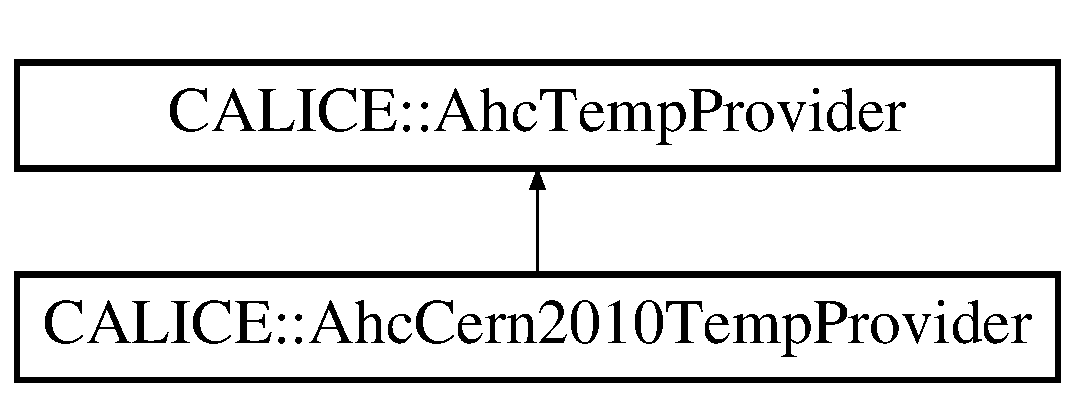
\includegraphics[height=2cm]{classCALICE_1_1AhcCern2010TempProvider}
\end{center}
\end{figure}
\subsection*{Public Member Functions}
\begin{DoxyCompactItemize}
\item 
{\bfseries AhcCern2010TempProvider} ({\bf AhcMapper} const $\ast$mapper)\label{classCALICE_1_1AhcCern2010TempProvider_a5e0bea69970f631796885bfa5e36d1ba}

\item 
void {\bfseries applyCorrection} ()\label{classCALICE_1_1AhcCern2010TempProvider_a4df8bc703a896c74956b470211396907}

\item 
float {\bf getSensorTemp} (int module, int sensor)
\begin{DoxyCompactList}\small\item\em Returns the temperature of the specified sensor in the given module. \item\end{DoxyCompactList}\item 
float {\bf getCellTemp} (int module, int chip, int chan)
\begin{DoxyCompactList}\small\item\em Returns the temperature for the cell in the specified module connected to the given chip and channel. \item\end{DoxyCompactList}\item 
float {\bf getCellTempError} (int module, int chip, int chan)
\begin{DoxyCompactList}\small\item\em Returns the error on the temperature for the cell in the specified module connected to the given chip and channel. \item\end{DoxyCompactList}\item 
float {\bf getAvgTemp} ()\label{classCALICE_1_1AhcCern2010TempProvider_ae70a7581cfb3f9e46fa6cf262cf4e945}

\begin{DoxyCompactList}\small\item\em Return the average calorimeter temperature. \item\end{DoxyCompactList}\item 
float {\bf getAvgModuleTemp} (unsigned module)\label{classCALICE_1_1AhcCern2010TempProvider_a18085f89099caedb30b3f341487c5db8}

\begin{DoxyCompactList}\small\item\em Return the average temperature for the specified module. \item\end{DoxyCompactList}\item 
int {\bf getSensor} (int chip, int chan)
\begin{DoxyCompactList}\small\item\em Returns the closest sensor to cell connected to chip, chan according to DESY-\/THESIS-\/2008-\/050. \item\end{DoxyCompactList}\end{DoxyCompactItemize}
\subsection*{Protected Member Functions}
\begin{DoxyCompactItemize}
\item 
void {\bfseries applyCorrectionForUnreasonableSensors} (int module, int sensor)\label{classCALICE_1_1AhcCern2010TempProvider_a2cffa40eb335c8c66de5d939328215ac}

\item 
bool {\bfseries applyCorrectionForUnreasonableModules} (int module, int sensor)\label{classCALICE_1_1AhcCern2010TempProvider_a36b34c7e212637d22e887a7bd8bf681c}

\end{DoxyCompactItemize}
\subsection*{Private Member Functions}
\begin{DoxyCompactItemize}
\item 
bool {\bfseries isModuleOff} (int module)\label{classCALICE_1_1AhcCern2010TempProvider_a2c784e8262e279884622c9a31ef504c8}

\item 
double {\bfseries median} (float a[$\,$], int n)\label{classCALICE_1_1AhcCern2010TempProvider_aee3afaa7ee7c7ed1a16b577f92033c49}

\end{DoxyCompactItemize}
\subsection*{Private Attributes}
\begin{DoxyCompactItemize}
\item 
{\bf AhcMapper} const $\ast$ {\bfseries \_\-mapper}\label{classCALICE_1_1AhcCern2010TempProvider_ac4824fa70b8bc9ad7c8eb6d58de6724f}

\item 
float {\bf \_\-calorimeterAverageTemperature}\label{classCALICE_1_1AhcCern2010TempProvider_a03d9619a42ad38435a85b93daeac3631}

\begin{DoxyCompactList}\small\item\em average temperature of the calorimeter \item\end{DoxyCompactList}\item 
float {\bfseries \_\-calorimeterAverageTemperatureRMS}\label{classCALICE_1_1AhcCern2010TempProvider_abd57ff9baed27c7e0459a11294ef4421}

\item 
float {\bfseries \_\-calorimeterAverageTemperatureCount}\label{classCALICE_1_1AhcCern2010TempProvider_a918fbf8455a23692314f0e913ad7cffa}

\item 
std::vector$<$ float $>$ {\bfseries \_\-moduleAverageTemperature}\label{classCALICE_1_1AhcCern2010TempProvider_a50ebabda787f8d5055938bb65edd7737}

\item 
std::vector$<$ float $>$ {\bfseries \_\-moduleAverageTemperatureRMS}\label{classCALICE_1_1AhcCern2010TempProvider_adb6bc09c87dfd5bc1aadc70d1bf56adb}

\item 
std::vector$<$ int $>$ {\bfseries \_\-moduleAverageTemperatureCount}\label{classCALICE_1_1AhcCern2010TempProvider_a6a78dcea2a8f624b2d425727626e5bd7}

\end{DoxyCompactItemize}


\subsection{Detailed Description}
This is a temperature provider for the AHCAL.based on the studies of the temperature profiles from CERN 2010 data. 

Definition at line 15 of file AhcCern2010TempProvider.hh.

\subsection{Member Function Documentation}
\index{CALICE::AhcCern2010TempProvider@{CALICE::AhcCern2010TempProvider}!getCellTemp@{getCellTemp}}
\index{getCellTemp@{getCellTemp}!CALICE::AhcCern2010TempProvider@{CALICE::AhcCern2010TempProvider}}
\subsubsection[{getCellTemp}]{\setlength{\rightskip}{0pt plus 5cm}float CALICE::AhcCern2010TempProvider::getCellTemp (int {\em module}, \/  int {\em chip}, \/  int {\em chan})\hspace{0.3cm}{\ttfamily  [virtual]}}\label{classCALICE_1_1AhcCern2010TempProvider_a50c27d4ce36e8bda65a50c41f3f55835}


Returns the temperature for the cell in the specified module connected to the given chip and channel. This is only the definition of the interface, a concrete funtion has to be implemented in a derived class. Note: Modules are counted from 1! The valid range for module numbers thus is 1 to 38. 

Implements {\bf CALICE::AhcTempProvider} \doxyref{}{p.}{classCALICE_1_1AhcTempProvider_aa12c75d45d7ade54316dd113a6bab2d1}.

Definition at line 29 of file AhcCern2010TempProvider.cc.

References getSensor(), CALICE::AhcTempProvider::newCalibCol, CALICE::AhcTempProvider::newSanityRange, CALICE::AhcTempProvider::newSroModCol, and CALICE::AhcTempProvider::sensorTemp.\index{CALICE::AhcCern2010TempProvider@{CALICE::AhcCern2010TempProvider}!getCellTempError@{getCellTempError}}
\index{getCellTempError@{getCellTempError}!CALICE::AhcCern2010TempProvider@{CALICE::AhcCern2010TempProvider}}
\subsubsection[{getCellTempError}]{\setlength{\rightskip}{0pt plus 5cm}float CALICE::AhcCern2010TempProvider::getCellTempError (int {\em module}, \/  int {\em chip}, \/  int {\em chan})\hspace{0.3cm}{\ttfamily  [virtual]}}\label{classCALICE_1_1AhcCern2010TempProvider_a49df2cbe0a0e947fc69fc2f9e6d4af7e}


Returns the error on the temperature for the cell in the specified module connected to the given chip and channel. This is only the definition of the interface, a concrete funtion has to be implemented in a derived class. Note: Modules are counted from 1! The valid range for module numbers thus is 1 to 38. 

Implements {\bf CALICE::AhcTempProvider} \doxyref{}{p.}{classCALICE_1_1AhcTempProvider_a72d155c16a772198a0587886e8d56102}.

Definition at line 51 of file AhcCern2010TempProvider.cc.

References getSensor(), CALICE::AhcTempProvider::newCalibCol, CALICE::AhcTempProvider::newSanityRange, CALICE::AhcTempProvider::newSroModCol, and CALICE::AhcTempProvider::sensorTempError.\index{CALICE::AhcCern2010TempProvider@{CALICE::AhcCern2010TempProvider}!getSensor@{getSensor}}
\index{getSensor@{getSensor}!CALICE::AhcCern2010TempProvider@{CALICE::AhcCern2010TempProvider}}
\subsubsection[{getSensor}]{\setlength{\rightskip}{0pt plus 5cm}int CALICE::AhcCern2010TempProvider::getSensor (int {\em chip}, \/  int {\em chan})}\label{classCALICE_1_1AhcCern2010TempProvider_a40cf8afb0b47f06a62959c3116b11dd8}


Returns the closest sensor to cell connected to chip, chan according to DESY-\/THESIS-\/2008-\/050. For the connection between the tile, chip and temperature sensors numbers, see {\tt http://www.desy.de/$\sim$richters/IJ-\/to-\/chip-\/channel/} 

Definition at line 74 of file AhcCern2010TempProvider.cc.

Referenced by getCellTemp(), and getCellTempError().\index{CALICE::AhcCern2010TempProvider@{CALICE::AhcCern2010TempProvider}!getSensorTemp@{getSensorTemp}}
\index{getSensorTemp@{getSensorTemp}!CALICE::AhcCern2010TempProvider@{CALICE::AhcCern2010TempProvider}}
\subsubsection[{getSensorTemp}]{\setlength{\rightskip}{0pt plus 5cm}float CALICE::AhcCern2010TempProvider::getSensorTemp (int {\em module}, \/  int {\em sensor})\hspace{0.3cm}{\ttfamily  [virtual]}}\label{classCALICE_1_1AhcCern2010TempProvider_ab8220e0d64d2785cc896beae3db00e12}


Returns the temperature of the specified sensor in the given module. 

Implements {\bf CALICE::AhcTempProvider} \doxyref{}{p.}{classCALICE_1_1AhcTempProvider_a9db9d635f879ed75ae983bbeca800ff8}.

Definition at line 490 of file AhcCern2010TempProvider.cc.

References CALICE::AhcTempProvider::newCalibCol, CALICE::AhcTempProvider::newSanityRange, CALICE::AhcTempProvider::newSroModCol, and CALICE::AhcTempProvider::sensorTemp.

The documentation for this class was generated from the following files:\begin{DoxyCompactItemize}
\item 
AhcCern2010TempProvider.hh\item 
AhcCern2010TempProvider.cc\end{DoxyCompactItemize}

\section{CALICE::AhcConditions Class Reference}
\label{classCALICE_1_1AhcConditions}\index{CALICE::AhcConditions@{CALICE::AhcConditions}}


Class for the \doxyref{CALICE}{p.}{namespaceCALICE} Ahcal conditions information during the reconstruction.  


{\ttfamily \#include $<$AhcConditions.hh$>$}\subsection*{Public Member Functions}
\begin{DoxyCompactItemize}
\item 
{\bf AhcConditions} ()\label{classCALICE_1_1AhcConditions_af6aea1e5d883dead6639e3be18b13f76}

\begin{DoxyCompactList}\small\item\em default constructor \item\end{DoxyCompactList}\item 
{\bf AhcConditions} (int moduleNr, unsigned moduleID, int calibStart, int calibWidth, bool calibEnable, int hold, int holdWidth, int multiplex, int vcalib, int verification, int sr[12])
\begin{DoxyCompactList}\small\item\em constructor, \doxyref{AhcConditions}{p.}{classCALICE_1_1AhcConditions} is initialized with the parameters given \item\end{DoxyCompactList}\item 
{\bfseries AhcConditions} (LCObject $\ast$obj)\label{classCALICE_1_1AhcConditions_ae1b844aa093496edbafaebc8f7c3e53e}

\item 
unsigned {\bf getModuleID} () const \label{classCALICE_1_1AhcConditions_afd54d91c0e7e95542cd9a625381c4c5a}

\begin{DoxyCompactList}\small\item\em get module ID of config \item\end{DoxyCompactList}\item 
unsigned {\bf getModuleNr} ()\label{classCALICE_1_1AhcConditions_ae8e8f7b251aa4c2d05259543b68eb774}

\begin{DoxyCompactList}\small\item\em get module number of config \item\end{DoxyCompactList}\item 
unsigned {\bf getCalibStart} () const \label{classCALICE_1_1AhcConditions_a2ac195704d21b51193059a17a5c2f1b4}

\begin{DoxyCompactList}\small\item\em get calib start \item\end{DoxyCompactList}\item 
unsigned {\bf getCalibWidth} () const \label{classCALICE_1_1AhcConditions_ab2bf4d8631141459c3d7091e88a7e72c}

\begin{DoxyCompactList}\small\item\em get calib width \item\end{DoxyCompactList}\item 
bool {\bf isCalibEnabled} () const \label{classCALICE_1_1AhcConditions_a8456b8157c53f61749215c47f536e24e}

\begin{DoxyCompactList}\small\item\em get if calib is enabled \item\end{DoxyCompactList}\item 
float {\bf getHold} () const \label{classCALICE_1_1AhcConditions_a725c4a0227fdb1a73859fcae2666f761}

\begin{DoxyCompactList}\small\item\em get hold \item\end{DoxyCompactList}\item 
unsigned {\bf getHoldWidth} () const \label{classCALICE_1_1AhcConditions_a1e08962a2ddb922dbcfaf88fac024662}

\begin{DoxyCompactList}\small\item\em get hold width \item\end{DoxyCompactList}\item 
unsigned {\bf getMultiplex} () const \label{classCALICE_1_1AhcConditions_abc2849f2554962e03e62d633afaa4553}

\begin{DoxyCompactList}\small\item\em get order of multiplexing \item\end{DoxyCompactList}\item 
unsigned {\bf getVcalib} () const \label{classCALICE_1_1AhcConditions_a7a3ebe5695fb349e015ddc12a4ab800f}

\begin{DoxyCompactList}\small\item\em get vcalib \item\end{DoxyCompactList}\item 
unsigned {\bf getVerification} () const \label{classCALICE_1_1AhcConditions_a792d5b3e5a9b31e40ffe9ea0c38a062a}

\begin{DoxyCompactList}\small\item\em get verification data \item\end{DoxyCompactList}\item 
unsigned {\bf getSR} (unsigned hab) const \label{classCALICE_1_1AhcConditions_a1521056060193303fb7c85657a005c1e}

\begin{DoxyCompactList}\small\item\em get hab sr \item\end{DoxyCompactList}\item 
void {\bf print} (std::ostream \&os)\label{classCALICE_1_1AhcConditions_a742f77cfa0886de4f4ff2ee0bde9900d}

\begin{DoxyCompactList}\small\item\em convenient print method \item\end{DoxyCompactList}\item 
const std::string {\bf getTypeName} () const \label{classCALICE_1_1AhcConditions_a6c7d11954356e9c4ac64a46525bb54ff}

\begin{DoxyCompactList}\small\item\em return the type of the class \item\end{DoxyCompactList}\item 
const std::string {\bf getDataDescription} () const \label{classCALICE_1_1AhcConditions_a31282cd05d783c18c6593f731e9fa24d}

\begin{DoxyCompactList}\small\item\em return a brief description of the data memeber \item\end{DoxyCompactList}\end{DoxyCompactItemize}


\subsection{Detailed Description}
Class for the \doxyref{CALICE}{p.}{namespaceCALICE} Ahcal conditions information during the reconstruction. renamed from \doxyref{CaliceConditions}{p.}{classCALICE_1_1CaliceConditions} 2007/12/14 B.Lutz

Information is stored module wise \begin{DoxyAuthor}{Author}
B. Lutz DESY 
\end{DoxyAuthor}
\begin{DoxyDate}{Date}
Sep 11 2006 
\end{DoxyDate}


Definition at line 32 of file AhcConditions.hh.

\subsection{Constructor \& Destructor Documentation}
\index{CALICE::AhcConditions@{CALICE::AhcConditions}!AhcConditions@{AhcConditions}}
\index{AhcConditions@{AhcConditions}!CALICE::AhcConditions@{CALICE::AhcConditions}}
\subsubsection[{AhcConditions}]{\setlength{\rightskip}{0pt plus 5cm}CALICE::AhcConditions::AhcConditions (int {\em moduleNr}, \/  unsigned {\em moduleID}, \/  int {\em calibStart}, \/  int {\em calibWidth}, \/  bool {\em calibEnable}, \/  int {\em hold}, \/  int {\em holdWidth}, \/  int {\em multiplex}, \/  int {\em vcalib}, \/  int {\em verification}, \/  int {\em sr}[12])\hspace{0.3cm}{\ttfamily  [inline]}}\label{classCALICE_1_1AhcConditions_a51eb529321a6006fb0b9d46046ba056a}


constructor, \doxyref{AhcConditions}{p.}{classCALICE_1_1AhcConditions} is initialized with the parameters given 
\begin{DoxyParams}{Parameters}
\item[{\em moduleNr}]mdoule \char`\"{}stamp\char`\"{} \item[{\em moduleID}]module ID of the module the hit is in, low byte gives upper or lower half, high byte gives module \char`\"{}stamp\char`\"{}, used to find correct calibration \item[{\em calibStart}]starting time of Tcalib signal in ticks \item[{\em calibWidth}]duration of the Tcalib signal in ticks \item[{\em calibEnable}]has Tcalib signal been sent at all? \item[{\em hold}]starting time of the hold signal in ticks (6.25ns) \item[{\em holdWidth}]duration of the hold signal in ticks (6.25ns) \item[{\em multiplex}]number of multiplexed signals in the acquisition cycle \item[{\em vcalib}]Vcalib value \item[{\em verification}]shift register verification pattern \item[{\em sr}]shift registers \end{DoxyParams}


Definition at line 54 of file AhcConditions.hh.

The documentation for this class was generated from the following files:\begin{DoxyCompactItemize}
\item 
AhcConditions.hh\item 
AhcConditions.cc\end{DoxyCompactItemize}

\section{CALICE::AhcMapper Class Reference}
\label{classCALICE_1_1AhcMapper}\index{CALICE::AhcMapper@{CALICE::AhcMapper}}


AHCAL implementation of \doxyref{Mapper}{p.}{classCALICE_1_1Mapper} class.  


{\ttfamily \#include $<$AhcMapper.hh$>$}Inheritance diagram for CALICE::AhcMapper::\begin{figure}[H]
\begin{center}
\leavevmode
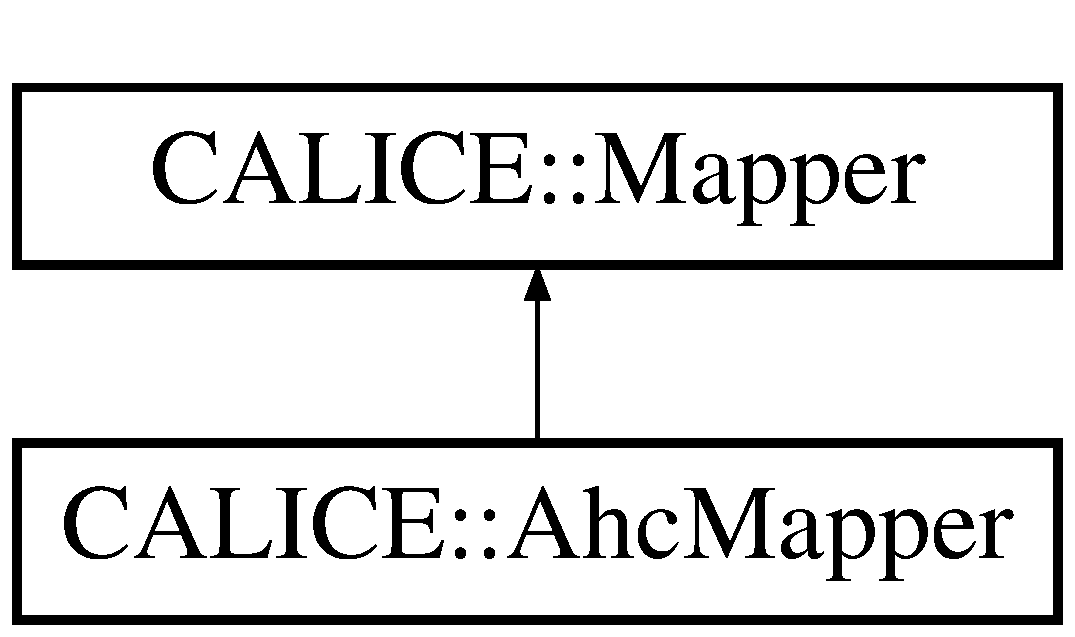
\includegraphics[height=2cm]{classCALICE_1_1AhcMapper}
\end{center}
\end{figure}
\subsection*{Public Member Functions}
\begin{DoxyCompactItemize}
\item 
int {\bf getCellIDFromModChipChan} (const unsigned int module, const unsigned int chip, const unsigned int channel) const 
\begin{DoxyCompactList}\small\item\em generate (Mokka) cellID from module, chip, channel \item\end{DoxyCompactList}\item 
unsigned int {\bf getModuleFromCellID} (const int cellID) const 
\begin{DoxyCompactList}\small\item\em module number from (Mokka) CellID \item\end{DoxyCompactList}\item 
unsigned int {\bf getModuleFromDAQID} (const int DAQchannel) const 
\begin{DoxyCompactList}\small\item\em module number from DAQ channel ID \item\end{DoxyCompactList}\item 
unsigned int {\bf getModule} (const unsigned int crate, const unsigned int slot, const unsigned int fe) const 
\begin{DoxyCompactList}\small\item\em module number from triple crate, slot, fe \item\end{DoxyCompactList}\item 
unsigned int {\bf getModule} (const unsigned int k) const 
\begin{DoxyCompactList}\small\item\em module number from K \item\end{DoxyCompactList}\item 
unsigned int {\bf getModuleFromCellID} (const int cellID, bool \&valid) const 
\begin{DoxyCompactList}\small\item\em get module (number) in which this cell is included from (Mokka) cellID \item\end{DoxyCompactList}\item 
unsigned int {\bf getModuleFromDAQID} (const int DAQchannel, bool \&valid) const 
\begin{DoxyCompactList}\small\item\em get module (number) in which this (DAQ) channel is included \item\end{DoxyCompactList}\item 
unsigned int {\bf getModuleFromModuleID} (const int moduleID, bool \&valid) const 
\begin{DoxyCompactList}\small\item\em get module (number) from this (module) channel ID \item\end{DoxyCompactList}\item 
unsigned int {\bf getChipFromCellID} (const int cellID) const 
\begin{DoxyCompactList}\small\item\em chip number from (Mokka) CellID \item\end{DoxyCompactList}\item 
unsigned int {\bf getChip} (const unsigned int i, const unsigned int j, const unsigned int k) const 
\begin{DoxyCompactList}\small\item\em chip number from triple I, J, K \item\end{DoxyCompactList}\item 
unsigned int {\bf getChanFromCellID} (const int cellID) const 
\begin{DoxyCompactList}\small\item\em channel number from (Mokka) CellID \item\end{DoxyCompactList}\item 
unsigned int {\bf getChan} (const unsigned int i, const unsigned int j, const unsigned int k) const 
\begin{DoxyCompactList}\small\item\em chip number from triple I, J, K \item\end{DoxyCompactList}\item 
unsigned int {\bf getCrateFromCellID} (const int cellID) const 
\begin{DoxyCompactList}\small\item\em crate number from (Mokka) CellID \item\end{DoxyCompactList}\item 
unsigned int {\bf getCrateFromModuleID} (const int moduleID) const 
\begin{DoxyCompactList}\small\item\em crate number from Module cell ID \item\end{DoxyCompactList}\item 
unsigned int {\bf getCrate} (const unsigned int module) const 
\begin{DoxyCompactList}\small\item\em crate number from module number \item\end{DoxyCompactList}\item 
unsigned int {\bf getSlotFromCellID} (const int cellID) const 
\begin{DoxyCompactList}\small\item\em slot number from (Mokka) CellID \item\end{DoxyCompactList}\item 
unsigned int {\bf getSlotFromModuleID} (const int moduleID) const 
\begin{DoxyCompactList}\small\item\em slot number from Module cell ID \item\end{DoxyCompactList}\item 
unsigned int {\bf getSlot} (const unsigned int module) const 
\begin{DoxyCompactList}\small\item\em slot number from module number \item\end{DoxyCompactList}\item 
unsigned int {\bf getFeFromCellID} (const int cellID) const 
\begin{DoxyCompactList}\small\item\em front end number from (Mokka) CellID \item\end{DoxyCompactList}\item 
unsigned int {\bf getFeFromModuleID} (const int moduleID) const 
\begin{DoxyCompactList}\small\item\em front end number from Module cell ID \item\end{DoxyCompactList}\item 
unsigned int {\bf getFe} (const unsigned int module) const 
\begin{DoxyCompactList}\small\item\em front end number from module number \item\end{DoxyCompactList}\item 
unsigned int {\bf getIFromModuleID} (const int moduleID) const 
\begin{DoxyCompactList}\small\item\em I of (Mokka) cellID. \item\end{DoxyCompactList}\item 
unsigned int {\bf getIFromDAQID} (const int DAQchannel) const 
\begin{DoxyCompactList}\small\item\em I of (Mokka) cellID. \item\end{DoxyCompactList}\item 
unsigned int {\bf getI} (const unsigned int module, const unsigned int chip, const unsigned int chan) const 
\begin{DoxyCompactList}\small\item\em I of (Mokka) cellID. \item\end{DoxyCompactList}\item 
unsigned int {\bf getJFromModuleID} (const int moduleID) const 
\begin{DoxyCompactList}\small\item\em J of (Mokka) cellID. \item\end{DoxyCompactList}\item 
unsigned int {\bf getJFromDAQID} (const int DAQchannel) const 
\begin{DoxyCompactList}\small\item\em J of (Mokka) cellID. \item\end{DoxyCompactList}\item 
unsigned int {\bf getJ} (const unsigned int module, const unsigned chip, const unsigned chan) const 
\begin{DoxyCompactList}\small\item\em J of (Mokka) cellID. \item\end{DoxyCompactList}\item 
unsigned int {\bf getKFromModuleID} (const int moduleID) const 
\begin{DoxyCompactList}\small\item\em K of (Mokka) cellID. \item\end{DoxyCompactList}\item 
unsigned int {\bf getKFromDAQID} (const int DAQchannel) const 
\begin{DoxyCompactList}\small\item\em K of (Mokka) cellID. \item\end{DoxyCompactList}\item 
unsigned int {\bf getK} (const unsigned int module) const 
\begin{DoxyCompactList}\small\item\em K of (Mokka) cellID. \item\end{DoxyCompactList}\item 
unsigned int {\bf getISizeFromCellID} (const int cellID) const 
\begin{DoxyCompactList}\small\item\em get cell size in I direction of (Mokka) CellID coordinate \item\end{DoxyCompactList}\item 
unsigned int {\bf getISizeFromModuleID} (const int moduleID) const 
\begin{DoxyCompactList}\small\item\em get cell size in I direction of (Mokka) CellID coordinate \item\end{DoxyCompactList}\item 
unsigned int {\bf getISizeFromDAQID} (const int DAQchannel) const 
\begin{DoxyCompactList}\small\item\em get cell size in I direction of (Mokka) CellID coordinate \item\end{DoxyCompactList}\item 
unsigned int {\bf getISizeFromIJK} (const unsigned int i, const unsigned int j, const unsigned int k) const 
\begin{DoxyCompactList}\small\item\em get cell size in I direction of (Mokka) CellID coordinate \item\end{DoxyCompactList}\item 
unsigned int {\bf getISize} (const unsigned int module, const unsigned int chip, const unsigned int chan) const 
\begin{DoxyCompactList}\small\item\em get cell size in I direction of (Mokka) CellID coordinate \item\end{DoxyCompactList}\item 
unsigned int {\bf getJSizeFromCellID} (const int cellID) const 
\begin{DoxyCompactList}\small\item\em get cell size in J direction of (Mokka) CellID coordinate \item\end{DoxyCompactList}\item 
unsigned int {\bf getJSizeFromModuleID} (const int moduleID) const 
\begin{DoxyCompactList}\small\item\em get cell size in J direction of (Mokka) CellID coordinate \item\end{DoxyCompactList}\item 
unsigned int {\bf getJSizeFromDAQID} (const int DAQchannel) const 
\begin{DoxyCompactList}\small\item\em get cell size in J direction of (Mokka) CellID coordinate \item\end{DoxyCompactList}\item 
unsigned int {\bf getJSizeFromIJK} (const unsigned int i, const unsigned int j, const unsigned int k) const 
\begin{DoxyCompactList}\small\item\em get cell size in J direction of (Mokka) CellID coordinate \item\end{DoxyCompactList}\item 
unsigned int {\bf getJSize} (const unsigned int module, const unsigned int chip, const unsigned int chan) const 
\begin{DoxyCompactList}\small\item\em get cell size in J direction of (Mokka) CellID coordinate \item\end{DoxyCompactList}\item 
int {\bf getTrueCellID} (const int virtualCellIndex) const 
\begin{DoxyCompactList}\small\item\em return identifying index of cell \item\end{DoxyCompactList}\item 
int {\bf getTrueCellID} (const unsigned int i, const unsigned int j, const unsigned int k) const 
\begin{DoxyCompactList}\small\item\em return identifying index of cell \item\end{DoxyCompactList}\item 
unsigned int {\bf getTrueIFromCellID} (const int virtualCellID) const 
\begin{DoxyCompactList}\small\item\em return I of identifying index of cell \item\end{DoxyCompactList}\item 
unsigned int {\bf getTrueIFromIJK} (const unsigned int i, const unsigned int j, const unsigned int k) const 
\begin{DoxyCompactList}\small\item\em return I of identifying index of cell \item\end{DoxyCompactList}\item 
unsigned int {\bf getTrueI} (const unsigned int module, const unsigned int i, const unsigned int j) const 
\begin{DoxyCompactList}\small\item\em return I of identifying index of cell \item\end{DoxyCompactList}\item 
unsigned int {\bf getTrueJFromCellID} (const int virtualCellID) const 
\begin{DoxyCompactList}\small\item\em return J of identifying index of cell \item\end{DoxyCompactList}\item 
unsigned int {\bf getTrueJFromIJK} (const unsigned int i, const unsigned int j, const unsigned int k) const 
\begin{DoxyCompactList}\small\item\em return J of identifying index of cell \item\end{DoxyCompactList}\item 
unsigned int {\bf getTrueJ} (const unsigned int module, const unsigned int i, const unsigned int j) const 
\begin{DoxyCompactList}\small\item\em return J of identifying index of cell \item\end{DoxyCompactList}\item 
unsigned int {\bf getMaxModule} () const 
\begin{DoxyCompactList}\small\item\em return maximum module number \item\end{DoxyCompactList}\item 
unsigned int {\bf getMaxChip} () const 
\begin{DoxyCompactList}\small\item\em return maximum chip number \item\end{DoxyCompactList}\item 
unsigned int {\bf getMaxChannel} () const 
\begin{DoxyCompactList}\small\item\em return maximum channel number \item\end{DoxyCompactList}\item 
unsigned int {\bf getMaxI} () const 
\begin{DoxyCompactList}\small\item\em return maximum I index \item\end{DoxyCompactList}\item 
unsigned int {\bf getMaxJ} () const 
\begin{DoxyCompactList}\small\item\em return maximum J index \item\end{DoxyCompactList}\item 
unsigned int {\bf getMaxK} () const 
\begin{DoxyCompactList}\small\item\em return maximum K index \item\end{DoxyCompactList}\item 
void {\bf fill} (const lcio::LCCollection $\ast$moduleDescriptionCol, const lcio::LCCollection $\ast$moduleConnectionCol)
\begin{DoxyCompactList}\small\item\em fills all necessary mapping information \item\end{DoxyCompactList}\item 
void {\bf updateConnections} (const lcio::LCCollection $\ast$moduleConnectionCol)
\begin{DoxyCompactList}\small\item\em updates the mapping information in the class (possible after first fill only) \item\end{DoxyCompactList}\item 
void {\bf print} (std::ostream \&ostream) const 
\begin{DoxyCompactList}\small\item\em print current data contents \item\end{DoxyCompactList}\item 
void {\bf printStats} (std::ostream \&ostream) const 
\begin{DoxyCompactList}\small\item\em print summary of current data contents \item\end{DoxyCompactList}\end{DoxyCompactItemize}
\subsection*{Protected Member Functions}
\begin{DoxyCompactItemize}
\item 
unsigned int {\bf getIndexByCellID} (const int cellID) const 
\begin{DoxyCompactList}\small\item\em get a compact index for storing data in vectors \item\end{DoxyCompactList}\item 
unsigned int {\bf getIndexByDAQID} (const int ID) const 
\begin{DoxyCompactList}\small\item\em get a compact index for storing data in vectors \item\end{DoxyCompactList}\item 
unsigned int {\bf getIndexByModuleID} (const int ID) const 
\begin{DoxyCompactList}\small\item\em get a compact index for storing data in vectors \item\end{DoxyCompactList}\item 
unsigned int {\bf getMaxIndex} () const 
\begin{DoxyCompactList}\small\item\em get the maximum value of the compact index for storing data in vectors \item\end{DoxyCompactList}\item 
int {\bf getCellIDOfIndex} (unsigned int index) const 
\begin{DoxyCompactList}\small\item\em get the cell ID of a certain compact index \item\end{DoxyCompactList}\end{DoxyCompactItemize}
\subsection*{Private Types}
\begin{DoxyCompactItemize}
\item 
typedef std::map$<$ unsigned int, unsigned int $>$ {\bfseries indexMap\_\-t}\label{classCALICE_1_1AhcMapper_aeeed74906b2af733e9892f881e1e10f4}

\end{DoxyCompactItemize}
\subsection*{Private Member Functions}
\begin{DoxyCompactItemize}
\item 
bool {\bfseries valid} (const unsigned int index, const std::vector$<$ bool $>$ \&availableVec) const \label{classCALICE_1_1AhcMapper_a74df7b7905102cd68455c8fbb1b69d7e}

\item 
bool {\bfseries valid} (const unsigned int index, const indexMap\_\-t \&indexMap) const \label{classCALICE_1_1AhcMapper_aa9eeded28b325b54d4a532fc645e5af4}

\item 
unsigned int {\bfseries getModuleTypeIndex} (const unsigned int module) const \label{classCALICE_1_1AhcMapper_aab9e59fb5ea9b3796a01ad47d52bc1f6}

\item 
unsigned int {\bfseries getIndexModuleConnection} (const unsigned int crate, const unsigned int slot, const unsigned int fe) const \label{classCALICE_1_1AhcMapper_a8971d066c71198c8bf247bfee592349a}

\item 
unsigned int {\bfseries getCrateFromModuleConnectionIndex} (const unsigned int index) const \label{classCALICE_1_1AhcMapper_a3222ce7720aef1e7731426231e433452}

\item 
unsigned int {\bfseries getSlotFromModuleConnectionIndex} (const unsigned int index) const \label{classCALICE_1_1AhcMapper_a9b25bfccd367acde37bae9b90e1d622e}

\item 
unsigned int {\bfseries getFeFromModuleConnectionIndex} (const unsigned int index) const \label{classCALICE_1_1AhcMapper_ad7258974e1fe5e8127b32b42619e2d1f}

\item 
unsigned int {\bfseries getCompactIndex} (const unsigned int module, const unsigned int chip, const unsigned int chan) const \label{classCALICE_1_1AhcMapper_aab353949bad76aaf654e41da8deae82c}

\item 
unsigned int {\bfseries getCompactIndex} (const unsigned int module, const unsigned int chanIndex) const \label{classCALICE_1_1AhcMapper_ae37272cef13cfad682728dafb3d2324a}

\item 
unsigned int {\bfseries getModuleFromCompactIndex} (const unsigned int index) const \label{classCALICE_1_1AhcMapper_ae9f81a2a43b50256d8950a11a88fa275}

\item 
unsigned int {\bfseries getChipFromCompactIndex} (const unsigned int index) const \label{classCALICE_1_1AhcMapper_ad18f22334b7691c9b60855d2d63008a3}

\item 
unsigned int {\bfseries getChanFromCompactIndex} (const unsigned int index) const \label{classCALICE_1_1AhcMapper_ae7a2539be4244d7fd0cdcf4afac85ad0}

\item 
unsigned int {\bfseries getModuleFromIndex} (const unsigned int index, bool \&valid) const \label{classCALICE_1_1AhcMapper_a56c48aba41a7c726a457c7653eeb1a5c}

\item 
unsigned int {\bfseries getIndexChan} (const unsigned int chip, const unsigned int chan) const \label{classCALICE_1_1AhcMapper_a4a8f47ef57d76bd9fb2c23f27a7c6451}

\item 
unsigned int {\bfseries getChipFromChanIndex} (const unsigned int index) const \label{classCALICE_1_1AhcMapper_a2324012066d0903ba23d5f96d35b1c78}

\item 
unsigned int {\bfseries getChanFromChanIndex} (const unsigned int index) const \label{classCALICE_1_1AhcMapper_ac06830ea38f15374a584208d4a40f86a}

\item 
unsigned int {\bfseries getIndexIJ} (const unsigned int i, const unsigned int j) const \label{classCALICE_1_1AhcMapper_a204172bf4005d14c1bd7b70df98186d3}

\item 
unsigned int {\bfseries getIFromIJIndex} (const unsigned int index) const \label{classCALICE_1_1AhcMapper_a32cb7e27e0ae8867fb64b3217e8b4dac}

\item 
unsigned int {\bfseries getJFromIJIndex} (const unsigned int index) const \label{classCALICE_1_1AhcMapper_adcd54575e64211dc80da66e269834daa}

\item 
void {\bfseries clearCrate} ()\label{classCALICE_1_1AhcMapper_aefa941cea97ef01e1f400fd82cbd36f8}

\item 
void {\bfseries clearSlot} ()\label{classCALICE_1_1AhcMapper_a79794d916def06030787c9f288aa2bad}

\item 
void {\bfseries clearModuleType} ()\label{classCALICE_1_1AhcMapper_a024182c2a5e1ad79e0a9de21fc8a11d7}

\item 
{\footnotesize template$<$class T $>$ }\\void {\bfseries initToSize} (std::vector$<$ T $>$ \&vec, const unsigned int size, const T initValue)\label{classCALICE_1_1AhcMapper_a821c963fd61c1ce4a060d80a26662549}

\item 
void {\bfseries initToSize} (std::vector$<$ bool $>$ \&vec, const unsigned int size)\label{classCALICE_1_1AhcMapper_a383c4627b641162bb5d7b78c60c3989a}

\item 
void {\bfseries initToSize} (std::vector$<$ unsigned int $>$ \&dataVec, std::vector$<$ bool $>$ \&availableVec, const unsigned int size)\label{classCALICE_1_1AhcMapper_ad6b97628b5c5e4db1fc12cee65cc3f4d}

\item 
void {\bfseries initFe} (const unsigned int maxFe=0)\label{classCALICE_1_1AhcMapper_ad15c4051d56f20ffc66e0b5d52f81890}

\item 
void {\bfseries initModule} (const unsigned int maxMod=0)\label{classCALICE_1_1AhcMapper_af15a8d86b8f3d9210b0899a0ee1f218e}

\item 
void {\bfseries initK} (const unsigned int maxK=0)\label{classCALICE_1_1AhcMapper_a76e45ca5b0e1e2706c49f6c8250a0d38}

\item 
void {\bfseries initIJChipChannel} (const unsigned int maxI=0, const unsigned int maxJ=0, const unsigned int maxChip=0, const unsigned int maxChan=0)\label{classCALICE_1_1AhcMapper_a65d452691dedf5bb9fecddf3bfb444b4}

\item 
void {\bfseries clear} ()\label{classCALICE_1_1AhcMapper_ac1442af64ad70eb7d0a1b7fc4c7f53b6}

\item 
void {\bfseries registerCrate} (const unsigned int crate)\label{classCALICE_1_1AhcMapper_ac58c61c50764da525db379b0d1fc9294}

\item 
bool {\bfseries crateAvailable} (const unsigned int crate) const \label{classCALICE_1_1AhcMapper_ae477476123f13062074f2b9c650bb9b1}

\item 
void {\bfseries registerSlot} (const unsigned int slot)\label{classCALICE_1_1AhcMapper_a41134f8aced6392e03c901a73ea9ee2a}

\item 
bool {\bfseries slotAvailable} (const unsigned int slot) const \label{classCALICE_1_1AhcMapper_a881f7bb684650d934f3e3f4712b89ee7}

\item 
void {\bfseries registerModuleType} (const unsigned int moduleTypeName)\label{classCALICE_1_1AhcMapper_a45518c038310ae5493d7012d40664725}

\item 
bool {\bfseries moduleTypeAvailable} (const unsigned int moduleTypeName) const \label{classCALICE_1_1AhcMapper_a81729b3b42e81d44cd31b29c95707f9e}

\item 
unsigned int {\bfseries countAvailable} (const std::vector$<$ bool $>$ \&vec) const \label{classCALICE_1_1AhcMapper_aac91ec43c8273688216ae604ac05e895}

\item 
void {\bfseries setModuleCrateSlotFe} (const unsigned int module, const unsigned int crate, const unsigned int slot, const unsigned int fe)\label{classCALICE_1_1AhcMapper_a4d3085baa30407cb160fc33c9c78bcd2}

\item 
void {\bfseries setModuleType} (const unsigned int module, const unsigned int typeName)\label{classCALICE_1_1AhcMapper_a2b871dd10848faae136940c12ca27bd9}

\item 
void {\bfseries setModuleK} (const unsigned int module, const unsigned int K)\label{classCALICE_1_1AhcMapper_a08953a9ae064d95675d9cd0a749570a6}

\item 
void {\bfseries setModuleTypeIJChipChannel} (const unsigned int moduleTypeName, const unsigned int I, const unsigned int J, const unsigned int sizeI, const unsigned int sizeJ, const unsigned int chip, const unsigned int channel)\label{classCALICE_1_1AhcMapper_a73d414346acc2e03052b22fabc050d86}

\item 
void {\bf fillModuleConnection} (const lcio::LCCollection $\ast$col)
\begin{DoxyCompactList}\small\item\em sets the mapping information in the class, call after fillModuleDescription \item\end{DoxyCompactList}\item 
void {\bf fillModuleDescription} (const lcio::LCCollection $\ast$col)
\begin{DoxyCompactList}\small\item\em sets the module layout information in the class, module connection information will be invalidated \item\end{DoxyCompactList}\item 
void {\bfseries getChipChannelForModuleDescriptionID} (const unsigned int id, const unsigned int moduleType, int \&chip, int \&channel) const \label{classCALICE_1_1AhcMapper_a8a11bbe860cd7085fbc975bfcc791c37}

\item 
unsigned int {\bfseries getCombinedModuleType} (const unsigned int moduleType) const \label{classCALICE_1_1AhcMapper_a8749cdfa53ef252ff887bfec78d5830b}

\item 
int {\bfseries correctCellIndex} (const unsigned int moduleType, const int cellIndex) const \label{classCALICE_1_1AhcMapper_a6469d9f7071f5ebb451530e41b5660a5}

\item 
const std::string {\bfseries printIfAvailable} (bool available, unsigned int value) const \label{classCALICE_1_1AhcMapper_ad775b776bc11616feafa9402b4d0f489}

\end{DoxyCompactItemize}
\subsection*{Private Attributes}
\begin{DoxyCompactItemize}
\item 
unsigned int {\bfseries \_\-nChan}\label{classCALICE_1_1AhcMapper_ad1223d57d472b9a1a47d0cdc58b2e4d7}

\item 
unsigned int {\bfseries \_\-nChip}\label{classCALICE_1_1AhcMapper_acca5e6401c3930c7bd0a629ee3f93178}

\item 
unsigned int {\bfseries \_\-nFe}\label{classCALICE_1_1AhcMapper_a0d39db3b164e7810a9ce1bec289a1410}

\item 
unsigned int {\bfseries \_\-nSlot}\label{classCALICE_1_1AhcMapper_a298cc6f721fe2a76514a49e83831f4e3}

\item 
unsigned int {\bfseries \_\-maxSlot}\label{classCALICE_1_1AhcMapper_a51ef6086881b08eb51ca5af2bdcfcf83}

\item 
unsigned int {\bfseries \_\-nCrate}\label{classCALICE_1_1AhcMapper_a012ef86ff01b044e8c33b9871ecbc4b3}

\item 
unsigned int {\bfseries \_\-nMod}\label{classCALICE_1_1AhcMapper_a1f91d835a24d504011715fc7cecd4a8e}

\item 
unsigned int {\bfseries \_\-nModType}\label{classCALICE_1_1AhcMapper_a30c33cb167b3062406eaa4a51ef5b64f}

\item 
unsigned int {\bfseries \_\-nI}\label{classCALICE_1_1AhcMapper_a1df3b36a1945b9e16283de7159f61a4e}

\item 
unsigned int {\bfseries \_\-nJ}\label{classCALICE_1_1AhcMapper_a2228494a778640c420afe67f81f4c030}

\item 
unsigned int {\bfseries \_\-nK}\label{classCALICE_1_1AhcMapper_aa20c4b918afca46a0315529efb2263a0}

\item 
indexMap\_\-t {\bfseries \_\-crateIndex}\label{classCALICE_1_1AhcMapper_a141fb6ec8b5c668ed3ad02edb89c8e0c}

\item 
std::vector$<$ unsigned int $>$ {\bfseries \_\-crateNumber}\label{classCALICE_1_1AhcMapper_a9bcc209bc9a2cd2208451d9e7e98168f}

\item 
std::vector$<$ unsigned int $>$ {\bfseries \_\-slotIndex}\label{classCALICE_1_1AhcMapper_a870803394fbfaf449dc5e3a9564abebf}

\item 
std::vector$<$ unsigned int $>$ {\bfseries \_\-slotNumber}\label{classCALICE_1_1AhcMapper_ad2acb33e40a070102170ba90c90ac5df}

\item 
std::vector$<$ bool $>$ {\bfseries \_\-slotAvailable}\label{classCALICE_1_1AhcMapper_ad45184245e1c6716113883282fee77ad}

\item 
std::vector$<$ bool $>$ {\bfseries \_\-connectionAvailable}\label{classCALICE_1_1AhcMapper_a0ef975b1772d9da449e18a94535a6ebc}

\item 
std::vector$<$ bool $>$ {\bfseries \_\-moduleAvailable}\label{classCALICE_1_1AhcMapper_a45ba28e98649b1f4956548e266537db3}

\item 
std::vector$<$ unsigned int $>$ {\bfseries \_\-typeVmodule}\label{classCALICE_1_1AhcMapper_a165279f2c79fc7bdaa6c5b33186d7174}

\item 
std::vector$<$ unsigned int $>$ {\bfseries \_\-connectionVmodule}\label{classCALICE_1_1AhcMapper_a210096c9fb1c3286b2a07e7fcfc3d1f8}

\item 
std::vector$<$ bool $>$ {\bfseries \_\-connectionVmoduleAvailable}\label{classCALICE_1_1AhcMapper_ad03313bc91520da24585f0e3c5f33342}

\item 
std::vector$<$ unsigned int $>$ {\bfseries \_\-moduleVconnection}\label{classCALICE_1_1AhcMapper_a9492ae109cabc3256c81d0ead4282422}

\item 
std::vector$<$ unsigned int $>$ {\bfseries \_\-kVmodule}\label{classCALICE_1_1AhcMapper_a6c6557dbf072ae4742a2ead776a24d33}

\item 
std::vector$<$ bool $>$ {\bfseries \_\-kVmoduleAvailable}\label{classCALICE_1_1AhcMapper_a16287dbcd49d1734cd458fd21e27b8fb}

\item 
std::vector$<$ unsigned int $>$ {\bfseries \_\-moduleVk}\label{classCALICE_1_1AhcMapper_a804a038a75c8576ba7e92546e7ef2354}

\item 
std::vector$<$ bool $>$ {\bfseries \_\-kAvailable}\label{classCALICE_1_1AhcMapper_a867fa2028b681d060300594a36ac71cd}

\item 
std::vector$<$ unsigned int $>$ {\bfseries \_\-moduleTypeName}\label{classCALICE_1_1AhcMapper_a1708a1be8814517d1f7a42367671228c}

\item 
std::vector$<$ unsigned int $>$ {\bfseries \_\-moduleTypeIndex}\label{classCALICE_1_1AhcMapper_abea6e5e1063923458a28fd310827d013}

\item 
std::vector$<$ bool $>$ {\bfseries \_\-moduleTypeAvailable}\label{classCALICE_1_1AhcMapper_ab94ebc350d70dc688045317888d9bd6d}

\item 
std::vector$<$ std::vector$<$ unsigned int $>$ $>$ {\bfseries \_\-ijVchan}\label{classCALICE_1_1AhcMapper_af9679ed2782209ef2ea4b487751d1707}

\item 
std::vector$<$ std::vector$<$ bool $>$ $>$ {\bfseries \_\-chipChanAvailable}\label{classCALICE_1_1AhcMapper_a4d7169258a2dfcf9539c3ace81a51585}

\item 
std::vector$<$ std::vector$<$ unsigned int $>$ $>$ {\bfseries \_\-chanVij}\label{classCALICE_1_1AhcMapper_a8437e5029df0527ee3f54daf75e3c42b}

\item 
std::vector$<$ std::vector$<$ bool $>$ $>$ {\bfseries \_\-ijAvailable}\label{classCALICE_1_1AhcMapper_aad90e93df3179242870ac3ee1487381f}

\item 
std::vector$<$ std::vector$<$ bool $>$ $>$ {\bfseries \_\-ijSecondaryAvailable}\label{classCALICE_1_1AhcMapper_afc9cff60e5249739c91ea2a157259a6d}

\item 
std::vector$<$ std::vector$<$ unsigned int $>$ $>$ {\bfseries \_\-sizeIVchan}\label{classCALICE_1_1AhcMapper_a111d0fbbace0b66fe60eb42f338d7aba}

\item 
std::vector$<$ std::vector$<$ unsigned int $>$ $>$ {\bfseries \_\-sizeJVchan}\label{classCALICE_1_1AhcMapper_a55efa1152aec0daed30ad88b32c726ec}

\end{DoxyCompactItemize}


\subsection{Detailed Description}
AHCAL implementation of \doxyref{Mapper}{p.}{classCALICE_1_1Mapper} class. \begin{DoxyParagraph}{invalid cells and exception handling}
Most functions throw a \doxyref{CALICE::BadDataException}{p.}{classCALICE_1_1BadDataException} if an invalid combination or ID is queried. Not all invalid combinations will be detected by all commands, depending on the necessary coordinate transformations in the command. E.g.: When querying the module from a Mokka cell ID, only K is extracted from the ID. If no module exists for this K an exception is thrown. But there will be no exception thrown if K is valid but I and J belong to a channel which does not exist in this module.
\end{DoxyParagraph}
\begin{DoxyParagraph}{}
The protected getIndexFunctions do {\bfseries not} throw exceptions to allow a fast lookup of the index. Invalid channels are signalled with return value maxIndex+1.
\end{DoxyParagraph}
\begin{DoxyParagraph}{}
Some functions have a second version that does a full check if the ID is valid without throwing an exception.
\end{DoxyParagraph}
\begin{DoxyAuthor}{Author}
{\tt Benjamin.Lutz@desy.de} 
\end{DoxyAuthor}
\begin{DoxyVersion}{Version}
0.3 
\end{DoxyVersion}
\begin{DoxyDate}{Date}
January 2010 
\end{DoxyDate}


Definition at line 44 of file AhcMapper.hh.

\subsection{Member Function Documentation}
\index{CALICE::AhcMapper@{CALICE::AhcMapper}!fill@{fill}}
\index{fill@{fill}!CALICE::AhcMapper@{CALICE::AhcMapper}}
\subsubsection[{fill}]{\setlength{\rightskip}{0pt plus 5cm}void CALICE::AhcMapper::fill (const lcio::LCCollection $\ast$ {\em moduleDescriptionCol}, \/  const lcio::LCCollection $\ast$ {\em moduleConnectionCol})\hspace{0.3cm}{\ttfamily  [inline]}}\label{classCALICE_1_1AhcMapper_ae4ab5d3a50a6105fb3fadb021790e46a}


fills all necessary mapping information Module layout types are set from moduleDescription (chip,channel to I,J,K \& size) Module connections are set from moduleConnection (crate, slot, fe to module)

Old settings are cleared before new are set.


\begin{DoxyParams}{Parameters}
\item[\mbox{$\leftarrow$} {\em moduleDescriptionCol}]LCGenericObject collection of \doxyref{ModuleDescription}{p.}{classCALICE_1_1ModuleDescription} type \item[\mbox{$\leftarrow$} {\em moduleConnectionCol}]LCGenericObject collection of \doxyref{ModuleConnection}{p.}{classCALICE_1_1ModuleConnection} type \end{DoxyParams}


Definition at line 937 of file AhcMapper.hh.

References fillModuleConnection(), and fillModuleDescription().\index{CALICE::AhcMapper@{CALICE::AhcMapper}!fillModuleConnection@{fillModuleConnection}}
\index{fillModuleConnection@{fillModuleConnection}!CALICE::AhcMapper@{CALICE::AhcMapper}}
\subsubsection[{fillModuleConnection}]{\setlength{\rightskip}{0pt plus 5cm}void CALICE::AhcMapper::fillModuleConnection (const lcio::LCCollection $\ast$ {\em col})\hspace{0.3cm}{\ttfamily  [private]}}\label{classCALICE_1_1AhcMapper_ac73575dd541b8d4a392dfd6c60aa0da7}


sets the mapping information in the class, call after fillModuleDescription The internal mapping of modules to type and electronics connection is set.


\begin{DoxyParams}{Parameters}
\item[\mbox{$\leftarrow$} {\em col}]LCGenericObject collection of \doxyref{ModuleConnection}{p.}{classCALICE_1_1ModuleConnection} type \end{DoxyParams}


Definition at line 15 of file AhcMapper.cc.

References CALICE::Mapper::mappingModified().

Referenced by fill(), and updateConnections().\index{CALICE::AhcMapper@{CALICE::AhcMapper}!fillModuleDescription@{fillModuleDescription}}
\index{fillModuleDescription@{fillModuleDescription}!CALICE::AhcMapper@{CALICE::AhcMapper}}
\subsubsection[{fillModuleDescription}]{\setlength{\rightskip}{0pt plus 5cm}void CALICE::AhcMapper::fillModuleDescription (const lcio::LCCollection $\ast$ {\em col})\hspace{0.3cm}{\ttfamily  [private]}}\label{classCALICE_1_1AhcMapper_a82a573535ff437f989ecc52d2e8a7f8e}


sets the module layout information in the class, module connection information will be invalidated The internal layout of modules, like channel to I,J,K and cell sizes are set.

\begin{DoxyWarning}{Warning}
module connection information will be invalidated, fillModuleConnection has to be called aftwards
\end{DoxyWarning}

\begin{DoxyParams}{Parameters}
\item[\mbox{$\leftarrow$} {\em col}]LCGenericObject collection of \doxyref{ModuleDescription}{p.}{classCALICE_1_1ModuleDescription} type \end{DoxyParams}


Definition at line 121 of file AhcMapper.cc.

References CALICE::CellIndex::getPadColumn(), CALICE::CellIndex::getPadRow(), and CALICE::Mapper::mappingModified().

Referenced by fill().\index{CALICE::AhcMapper@{CALICE::AhcMapper}!getCellIDOfIndex@{getCellIDOfIndex}}
\index{getCellIDOfIndex@{getCellIDOfIndex}!CALICE::AhcMapper@{CALICE::AhcMapper}}
\subsubsection[{getCellIDOfIndex}]{\setlength{\rightskip}{0pt plus 5cm}int CALICE::AhcMapper::getCellIDOfIndex (unsigned int {\em index}) const\hspace{0.3cm}{\ttfamily  [inline, protected, virtual]}}\label{classCALICE_1_1AhcMapper_af53a274b50f0f75e632454a4072113eb}


get the cell ID of a certain compact index \begin{DoxyWarning}{Warning}
This cell ID will only contain information about I, J and K. If the encoding string contains additional fields this will have value 0.
\end{DoxyWarning}
\begin{DoxySeeAlso}{See also}
setCellIDencoding
\end{DoxySeeAlso}
\begin{DoxyReturn}{Returns}
(Mokka) cell ID 
\end{DoxyReturn}


Implements {\bf CALICE::Mapper} \doxyref{}{p.}{group__CellIDgroup_ga1157f15cfe97ad035e6f6fb2fd32ce2e}.

Definition at line 1061 of file AhcMapper.hh.

References CALICE::DecoderSet::getCellID(), CALICE::Mapper::getDecoder(), getI(), getJ(), and getK().\index{CALICE::AhcMapper@{CALICE::AhcMapper}!getChan@{getChan}}
\index{getChan@{getChan}!CALICE::AhcMapper@{CALICE::AhcMapper}}
\subsubsection[{getChan}]{\setlength{\rightskip}{0pt plus 5cm}unsigned int CALICE::AhcMapper::getChan (const unsigned int {\em i}, \/  const unsigned int {\em j}, \/  const unsigned int {\em k}) const\hspace{0.3cm}{\ttfamily  [inline]}}\label{classCALICE_1_1AhcMapper_adbb5dfc3ce2df861b5ef96f6910bc287}


chip number from triple I, J, K 
\begin{DoxyParams}{Parameters}
\item[\mbox{$\leftarrow$} {\em i}]I \item[\mbox{$\leftarrow$} {\em j}]J \item[\mbox{$\leftarrow$} {\em k}]K\end{DoxyParams}

\begin{DoxyExceptions}{Exceptions}
\item[{\em \doxyref{BadDataException}{p.}{classCALICE_1_1BadDataException}}]if invalid channel\end{DoxyExceptions}
\begin{DoxyReturn}{Returns}
channel number 
\end{DoxyReturn}


Definition at line 255 of file AhcMapper.hh.

References getModule().

Referenced by getChanFromCellID(), getISizeFromIJK(), and getJSizeFromIJK().\index{CALICE::AhcMapper@{CALICE::AhcMapper}!getChip@{getChip}}
\index{getChip@{getChip}!CALICE::AhcMapper@{CALICE::AhcMapper}}
\subsubsection[{getChip}]{\setlength{\rightskip}{0pt plus 5cm}unsigned int CALICE::AhcMapper::getChip (const unsigned int {\em i}, \/  const unsigned int {\em j}, \/  const unsigned int {\em k}) const\hspace{0.3cm}{\ttfamily  [inline]}}\label{classCALICE_1_1AhcMapper_a4ff7ad6e9ea5756c7599b204b6c17c76}


chip number from triple I, J, K 
\begin{DoxyParams}{Parameters}
\item[\mbox{$\leftarrow$} {\em i}]I \item[\mbox{$\leftarrow$} {\em j}]J \item[\mbox{$\leftarrow$} {\em k}]K\end{DoxyParams}

\begin{DoxyExceptions}{Exceptions}
\item[{\em \doxyref{BadDataException}{p.}{classCALICE_1_1BadDataException}}]if lookup fails\end{DoxyExceptions}
\begin{DoxyReturn}{Returns}
chip number 
\end{DoxyReturn}


Definition at line 219 of file AhcMapper.hh.

References getModule().

Referenced by getChipFromCellID(), getISizeFromIJK(), and getJSizeFromIJK().\index{CALICE::AhcMapper@{CALICE::AhcMapper}!getCrate@{getCrate}}
\index{getCrate@{getCrate}!CALICE::AhcMapper@{CALICE::AhcMapper}}
\subsubsection[{getCrate}]{\setlength{\rightskip}{0pt plus 5cm}unsigned int CALICE::AhcMapper::getCrate (const unsigned int {\em module}) const\hspace{0.3cm}{\ttfamily  [inline]}}\label{classCALICE_1_1AhcMapper_a5b28fe8764726c1b30d64e44195bdb5c}


crate number from module number 
\begin{DoxyParams}{Parameters}
\item[\mbox{$\leftarrow$} {\em module}]module number\end{DoxyParams}

\begin{DoxyExceptions}{Exceptions}
\item[{\em \doxyref{BadDataException}{p.}{classCALICE_1_1BadDataException}}]if lookup fails\end{DoxyExceptions}
\begin{DoxyReturn}{Returns}
crate number 
\end{DoxyReturn}


Definition at line 303 of file AhcMapper.hh.

Referenced by getCrateFromCellID(), getCrateFromModuleID(), and print().\index{CALICE::AhcMapper@{CALICE::AhcMapper}!getFe@{getFe}}
\index{getFe@{getFe}!CALICE::AhcMapper@{CALICE::AhcMapper}}
\subsubsection[{getFe}]{\setlength{\rightskip}{0pt plus 5cm}unsigned int CALICE::AhcMapper::getFe (const unsigned int {\em module}) const\hspace{0.3cm}{\ttfamily  [inline]}}\label{classCALICE_1_1AhcMapper_ae612d629678ea13991d810f3a72b4c96}


front end number from module number 
\begin{DoxyParams}{Parameters}
\item[\mbox{$\leftarrow$} {\em module}]module number\end{DoxyParams}

\begin{DoxyExceptions}{Exceptions}
\item[{\em \doxyref{BadDataException}{p.}{classCALICE_1_1BadDataException}}]if lookup fails\end{DoxyExceptions}
\begin{DoxyReturn}{Returns}
front end number 
\end{DoxyReturn}


Definition at line 390 of file AhcMapper.hh.

Referenced by getFeFromCellID(), getFeFromModuleID(), and print().\index{CALICE::AhcMapper@{CALICE::AhcMapper}!getI@{getI}}
\index{getI@{getI}!CALICE::AhcMapper@{CALICE::AhcMapper}}
\subsubsection[{getI}]{\setlength{\rightskip}{0pt plus 5cm}unsigned int CALICE::AhcMapper::getI (const unsigned int {\em module}, \/  const unsigned int {\em chip}, \/  const unsigned int {\em chan}) const\hspace{0.3cm}{\ttfamily  [inline]}}\label{classCALICE_1_1AhcMapper_ac64aa07b08160c003c6f02c4fa76746a}


I of (Mokka) cellID. 
\begin{DoxyParams}{Parameters}
\item[\mbox{$\leftarrow$} {\em module}]module number \item[\mbox{$\leftarrow$} {\em chip}]chip number \item[\mbox{$\leftarrow$} {\em chan}]channel number\end{DoxyParams}

\begin{DoxyExceptions}{Exceptions}
\item[{\em \doxyref{BadDataException}{p.}{classCALICE_1_1BadDataException}}]if lookup fails\end{DoxyExceptions}
\begin{DoxyReturn}{Returns}
I 
\end{DoxyReturn}


Definition at line 435 of file AhcMapper.hh.

Referenced by getCellIDFromModChipChan(), getCellIDOfIndex(), getIFromDAQID(), and getIFromModuleID().\index{CALICE::AhcMapper@{CALICE::AhcMapper}!getIndexByCellID@{getIndexByCellID}}
\index{getIndexByCellID@{getIndexByCellID}!CALICE::AhcMapper@{CALICE::AhcMapper}}
\subsubsection[{getIndexByCellID}]{\setlength{\rightskip}{0pt plus 5cm}unsigned int CALICE::AhcMapper::getIndexByCellID (const int {\em cellID}) const\hspace{0.3cm}{\ttfamily  [inline, protected, virtual]}}\label{classCALICE_1_1AhcMapper_a1e4072147112a446171c2892ebe8e3e2}


get a compact index for storing data in vectors 
\begin{DoxyParams}{Parameters}
\item[\mbox{$\leftarrow$} {\em cellID}](Mokka) cell ID \end{DoxyParams}
\begin{DoxyReturn}{Returns}
compact index 
\end{DoxyReturn}


Implements {\bf CALICE::Mapper} \doxyref{}{p.}{group__CellIDgroup_gaaa6d826a6990c070c769f9754d2fbb76}.

Definition at line 975 of file AhcMapper.hh.

References CALICE::Mapper::getDecoder(), CALICE::DecoderSet::getIFromCellID(), CALICE::DecoderSet::getJFromCellID(), CALICE::DecoderSet::getKFromCellID(), and getMaxIndex().

Referenced by getModuleFromCellID().\index{CALICE::AhcMapper@{CALICE::AhcMapper}!getIndexByDAQID@{getIndexByDAQID}}
\index{getIndexByDAQID@{getIndexByDAQID}!CALICE::AhcMapper@{CALICE::AhcMapper}}
\subsubsection[{getIndexByDAQID}]{\setlength{\rightskip}{0pt plus 5cm}unsigned int CALICE::AhcMapper::getIndexByDAQID (const int {\em ID}) const\hspace{0.3cm}{\ttfamily  [inline, protected, virtual]}}\label{classCALICE_1_1AhcMapper_a54a30bb2306d44a9ab0240593c7425a8}


get a compact index for storing data in vectors 
\begin{DoxyParams}{Parameters}
\item[\mbox{$\leftarrow$} {\em ID}]DAQ channel ID \end{DoxyParams}
\begin{DoxyReturn}{Returns}
compact index 
\end{DoxyReturn}


Implements {\bf CALICE::Mapper} \doxyref{}{p.}{group__DAQgroup_ga4c00b2760cd3e935bed9db2f3fd28b06}.

Definition at line 998 of file AhcMapper.hh.

References CALICE::DecoderSet::getChannelFromDAQID(), CALICE::DecoderSet::getChipFromDAQID(), CALICE::DecoderSet::getCrateFromDAQID(), CALICE::Mapper::getDecoder(), CALICE::DecoderSet::getFeFromDAQID(), getMaxIndex(), and CALICE::DecoderSet::getSlotFromDAQID().

Referenced by getModuleFromDAQID().\index{CALICE::AhcMapper@{CALICE::AhcMapper}!getIndexByModuleID@{getIndexByModuleID}}
\index{getIndexByModuleID@{getIndexByModuleID}!CALICE::AhcMapper@{CALICE::AhcMapper}}
\subsubsection[{getIndexByModuleID}]{\setlength{\rightskip}{0pt plus 5cm}unsigned int CALICE::AhcMapper::getIndexByModuleID (const int {\em ID}) const\hspace{0.3cm}{\ttfamily  [inline, protected, virtual]}}\label{classCALICE_1_1AhcMapper_aaa1748613f85f7573be51b7344c69a4e}


get a compact index for storing data in vectors 
\begin{DoxyParams}{Parameters}
\item[\mbox{$\leftarrow$} {\em ID}]Module channel ID \end{DoxyParams}
\begin{DoxyReturn}{Returns}
compact index 
\end{DoxyReturn}


Implements {\bf CALICE::Mapper} \doxyref{}{p.}{group__ModuleIDgroup_gad546fcc374c9168872a957d90d62bda3}.

Definition at line 1033 of file AhcMapper.hh.

References CALICE::DecoderSet::getChannelFromModuleID(), CALICE::DecoderSet::getChipFromModuleID(), CALICE::Mapper::getDecoder(), getMaxIndex(), and CALICE::DecoderSet::getModuleFromModuleID().

Referenced by getModuleFromModuleID().\index{CALICE::AhcMapper@{CALICE::AhcMapper}!getISize@{getISize}}
\index{getISize@{getISize}!CALICE::AhcMapper@{CALICE::AhcMapper}}
\subsubsection[{getISize}]{\setlength{\rightskip}{0pt plus 5cm}unsigned int CALICE::AhcMapper::getISize (const unsigned int {\em module}, \/  const unsigned int {\em chip}, \/  const unsigned int {\em chan}) const\hspace{0.3cm}{\ttfamily  [inline]}}\label{classCALICE_1_1AhcMapper_aca7b7a137d5df143f6ceac76b5b16989}


get cell size in I direction of (Mokka) CellID coordinate 
\begin{DoxyParams}{Parameters}
\item[\mbox{$\leftarrow$} {\em module}]module number \item[\mbox{$\leftarrow$} {\em chip}]chip number \item[\mbox{$\leftarrow$} {\em chan}]channel number\end{DoxyParams}
\begin{DoxyReturn}{Returns}
size in I
\end{DoxyReturn}

\begin{DoxyExceptions}{Exceptions}
\item[{\em \doxyref{BadDataException}{p.}{classCALICE_1_1BadDataException}}]if lookup fails \end{DoxyExceptions}


Definition at line 605 of file AhcMapper.hh.

Referenced by getISizeFromDAQID(), getISizeFromIJK(), and getISizeFromModuleID().\index{CALICE::AhcMapper@{CALICE::AhcMapper}!getISizeFromIJK@{getISizeFromIJK}}
\index{getISizeFromIJK@{getISizeFromIJK}!CALICE::AhcMapper@{CALICE::AhcMapper}}
\subsubsection[{getISizeFromIJK}]{\setlength{\rightskip}{0pt plus 5cm}unsigned int CALICE::AhcMapper::getISizeFromIJK (const unsigned int {\em i}, \/  const unsigned int {\em j}, \/  const unsigned int {\em k}) const\hspace{0.3cm}{\ttfamily  [inline]}}\label{classCALICE_1_1AhcMapper_ad8568ed214d5cfc81b89b0718eeb07dc}


get cell size in I direction of (Mokka) CellID coordinate 
\begin{DoxyParams}{Parameters}
\item[\mbox{$\leftarrow$} {\em i}]I \item[\mbox{$\leftarrow$} {\em j}]J \item[\mbox{$\leftarrow$} {\em k}]K\end{DoxyParams}
\begin{DoxyReturn}{Returns}
size in I
\end{DoxyReturn}

\begin{DoxyExceptions}{Exceptions}
\item[{\em \doxyref{BadDataException}{p.}{classCALICE_1_1BadDataException}}]if lookup fails \end{DoxyExceptions}


Definition at line 591 of file AhcMapper.hh.

References getChan(), getChip(), getISize(), and getModule().

Referenced by getISizeFromCellID().\index{CALICE::AhcMapper@{CALICE::AhcMapper}!getJ@{getJ}}
\index{getJ@{getJ}!CALICE::AhcMapper@{CALICE::AhcMapper}}
\subsubsection[{getJ}]{\setlength{\rightskip}{0pt plus 5cm}unsigned int CALICE::AhcMapper::getJ (const unsigned int {\em module}, \/  const unsigned {\em chip}, \/  const unsigned {\em chan}) const\hspace{0.3cm}{\ttfamily  [inline]}}\label{classCALICE_1_1AhcMapper_ab02fce56e98d645a365eb23ba30afd4a}


J of (Mokka) cellID. 
\begin{DoxyParams}{Parameters}
\item[\mbox{$\leftarrow$} {\em module}]module number \item[\mbox{$\leftarrow$} {\em chip}]chip number \item[\mbox{$\leftarrow$} {\em chan}]channel number\end{DoxyParams}

\begin{DoxyExceptions}{Exceptions}
\item[{\em \doxyref{BadDataException}{p.}{classCALICE_1_1BadDataException}}]if lookup fails\end{DoxyExceptions}
\begin{DoxyReturn}{Returns}
J 
\end{DoxyReturn}


Definition at line 484 of file AhcMapper.hh.

Referenced by getCellIDFromModChipChan(), getCellIDOfIndex(), getJFromDAQID(), and getJFromModuleID().\index{CALICE::AhcMapper@{CALICE::AhcMapper}!getJSize@{getJSize}}
\index{getJSize@{getJSize}!CALICE::AhcMapper@{CALICE::AhcMapper}}
\subsubsection[{getJSize}]{\setlength{\rightskip}{0pt plus 5cm}unsigned int CALICE::AhcMapper::getJSize (const unsigned int {\em module}, \/  const unsigned int {\em chip}, \/  const unsigned int {\em chan}) const\hspace{0.3cm}{\ttfamily  [inline]}}\label{classCALICE_1_1AhcMapper_a9d0ec772a24eb62b4538afbdec89a285}


get cell size in J direction of (Mokka) CellID coordinate 
\begin{DoxyParams}{Parameters}
\item[\mbox{$\leftarrow$} {\em module}]module number \item[\mbox{$\leftarrow$} {\em chip}]chip number \item[\mbox{$\leftarrow$} {\em chan}]channel number\end{DoxyParams}
\begin{DoxyReturn}{Returns}
size in J
\end{DoxyReturn}

\begin{DoxyExceptions}{Exceptions}
\item[{\em \doxyref{BadDataException}{p.}{classCALICE_1_1BadDataException}}]if lookup fails \end{DoxyExceptions}


Definition at line 683 of file AhcMapper.hh.

Referenced by getJSizeFromDAQID(), getJSizeFromIJK(), and getJSizeFromModuleID().\index{CALICE::AhcMapper@{CALICE::AhcMapper}!getJSizeFromIJK@{getJSizeFromIJK}}
\index{getJSizeFromIJK@{getJSizeFromIJK}!CALICE::AhcMapper@{CALICE::AhcMapper}}
\subsubsection[{getJSizeFromIJK}]{\setlength{\rightskip}{0pt plus 5cm}unsigned int CALICE::AhcMapper::getJSizeFromIJK (const unsigned int {\em i}, \/  const unsigned int {\em j}, \/  const unsigned int {\em k}) const\hspace{0.3cm}{\ttfamily  [inline]}}\label{classCALICE_1_1AhcMapper_a887299333957bbde8da9fed21d68c380}


get cell size in J direction of (Mokka) CellID coordinate 
\begin{DoxyParams}{Parameters}
\item[\mbox{$\leftarrow$} {\em i}]I \item[\mbox{$\leftarrow$} {\em j}]J \item[\mbox{$\leftarrow$} {\em k}]K\end{DoxyParams}
\begin{DoxyReturn}{Returns}
size in J
\end{DoxyReturn}

\begin{DoxyExceptions}{Exceptions}
\item[{\em \doxyref{BadDataException}{p.}{classCALICE_1_1BadDataException}}]if lookup fails \end{DoxyExceptions}


Definition at line 669 of file AhcMapper.hh.

References getChan(), getChip(), getJSize(), and getModule().

Referenced by getJSizeFromCellID().\index{CALICE::AhcMapper@{CALICE::AhcMapper}!getK@{getK}}
\index{getK@{getK}!CALICE::AhcMapper@{CALICE::AhcMapper}}
\subsubsection[{getK}]{\setlength{\rightskip}{0pt plus 5cm}unsigned int CALICE::AhcMapper::getK (const unsigned int {\em module}) const\hspace{0.3cm}{\ttfamily  [inline]}}\label{classCALICE_1_1AhcMapper_a086377eb0064aab3337e8f12fcf40fc3}


K of (Mokka) cellID. 
\begin{DoxyParams}{Parameters}
\item[\mbox{$\leftarrow$} {\em module}]module number\end{DoxyParams}
\begin{DoxyReturn}{Returns}
K
\end{DoxyReturn}

\begin{DoxyExceptions}{Exceptions}
\item[{\em \doxyref{BadDataException}{p.}{classCALICE_1_1BadDataException}}]if lookup fails \end{DoxyExceptions}


Definition at line 531 of file AhcMapper.hh.

Referenced by CALICE::AhcMedianFilterTempProvider::applyCorrection(), getCellIDFromModChipChan(), getCellIDOfIndex(), getKFromDAQID(), getKFromModuleID(), and print().\index{CALICE::AhcMapper@{CALICE::AhcMapper}!getMaxIndex@{getMaxIndex}}
\index{getMaxIndex@{getMaxIndex}!CALICE::AhcMapper@{CALICE::AhcMapper}}
\subsubsection[{getMaxIndex}]{\setlength{\rightskip}{0pt plus 5cm}unsigned int CALICE::AhcMapper::getMaxIndex () const\hspace{0.3cm}{\ttfamily  [inline, protected, virtual]}}\label{classCALICE_1_1AhcMapper_a9b0644605c525dd581d8d8098764120e}


get the maximum value of the compact index for storing data in vectors \begin{DoxyReturn}{Returns}
maximum compact index 
\end{DoxyReturn}


Implements {\bf CALICE::Mapper} \doxyref{}{p.}{classCALICE_1_1Mapper_a34292aca2d87f6fc7f10094b5f7cab0e}.

Definition at line 1057 of file AhcMapper.hh.

Referenced by getIndexByCellID(), getIndexByDAQID(), and getIndexByModuleID().\index{CALICE::AhcMapper@{CALICE::AhcMapper}!getModule@{getModule}}
\index{getModule@{getModule}!CALICE::AhcMapper@{CALICE::AhcMapper}}
\subsubsection[{getModule}]{\setlength{\rightskip}{0pt plus 5cm}unsigned int CALICE::AhcMapper::getModule (const unsigned int {\em k}) const\hspace{0.3cm}{\ttfamily  [inline]}}\label{classCALICE_1_1AhcMapper_a602233d596480f6f4b4248ddf6370d36}


module number from K 
\begin{DoxyParams}{Parameters}
\item[\mbox{$\leftarrow$} {\em k}]K\end{DoxyParams}

\begin{DoxyExceptions}{Exceptions}
\item[{\em \doxyref{BadDataException}{p.}{classCALICE_1_1BadDataException}}]if lookup fails\end{DoxyExceptions}
\begin{DoxyReturn}{Returns}
module number 
\end{DoxyReturn}


Definition at line 135 of file AhcMapper.hh.

References CALICE::DecoderSet::getCellIDEncoding(), and CALICE::Mapper::getDecoder().\index{CALICE::AhcMapper@{CALICE::AhcMapper}!getModule@{getModule}}
\index{getModule@{getModule}!CALICE::AhcMapper@{CALICE::AhcMapper}}
\subsubsection[{getModule}]{\setlength{\rightskip}{0pt plus 5cm}unsigned int CALICE::AhcMapper::getModule (const unsigned int {\em crate}, \/  const unsigned int {\em slot}, \/  const unsigned int {\em fe}) const\hspace{0.3cm}{\ttfamily  [inline]}}\label{classCALICE_1_1AhcMapper_aab2c351390279b6ddb691922c1697b94}


module number from triple crate, slot, fe 
\begin{DoxyParams}{Parameters}
\item[\mbox{$\leftarrow$} {\em crate}]crate number (should be 0xac) \item[\mbox{$\leftarrow$} {\em slot}]slot number \item[\mbox{$\leftarrow$} {\em fe}]fe number\end{DoxyParams}
\begin{DoxyReturn}{Returns}
module number
\end{DoxyReturn}

\begin{DoxyExceptions}{Exceptions}
\item[{\em \doxyref{BadDataException}{p.}{classCALICE_1_1BadDataException}}]if lookup fails \end{DoxyExceptions}


Definition at line 118 of file AhcMapper.hh.

Referenced by getChan(), getChip(), getISizeFromIJK(), getJSizeFromIJK(), getModuleFromCellID(), getModuleFromDAQID(), getTrueIFromIJK(), and getTrueJFromIJK().\index{CALICE::AhcMapper@{CALICE::AhcMapper}!getSlot@{getSlot}}
\index{getSlot@{getSlot}!CALICE::AhcMapper@{CALICE::AhcMapper}}
\subsubsection[{getSlot}]{\setlength{\rightskip}{0pt plus 5cm}unsigned int CALICE::AhcMapper::getSlot (const unsigned int {\em module}) const\hspace{0.3cm}{\ttfamily  [inline]}}\label{classCALICE_1_1AhcMapper_a503f8cfd0f24380502c278adeb087015}


slot number from module number 
\begin{DoxyParams}{Parameters}
\item[\mbox{$\leftarrow$} {\em module}]module number\end{DoxyParams}

\begin{DoxyExceptions}{Exceptions}
\item[{\em \doxyref{BadDataException}{p.}{classCALICE_1_1BadDataException}}]if lookup fails\end{DoxyExceptions}
\begin{DoxyReturn}{Returns}
slot number 
\end{DoxyReturn}


Definition at line 346 of file AhcMapper.hh.

Referenced by getSlotFromCellID(), getSlotFromModuleID(), and print().\index{CALICE::AhcMapper@{CALICE::AhcMapper}!print@{print}}
\index{print@{print}!CALICE::AhcMapper@{CALICE::AhcMapper}}
\subsubsection[{print}]{\setlength{\rightskip}{0pt plus 5cm}void CALICE::AhcMapper::print (std::ostream \& {\em ostream}) const}\label{classCALICE_1_1AhcMapper_acb6947df0b876fd32cb206e576260fb9}


print current data contents A detailed printout of the current layout is sent to the given stream.


\begin{DoxyParams}{Parameters}
\item[\mbox{$\rightarrow$} {\em ostream}]stream for the output \end{DoxyParams}


Definition at line 286 of file AhcMapper.cc.

References getCrate(), getFe(), getK(), and getSlot().\index{CALICE::AhcMapper@{CALICE::AhcMapper}!printStats@{printStats}}
\index{printStats@{printStats}!CALICE::AhcMapper@{CALICE::AhcMapper}}
\subsubsection[{printStats}]{\setlength{\rightskip}{0pt plus 5cm}void CALICE::AhcMapper::printStats (std::ostream \& {\em ostream}) const}\label{classCALICE_1_1AhcMapper_aebe2a8845c6b24584f111009ef7f89c4}


print summary of current data contents A summary of the current number of module types, modules, etc... is printed.


\begin{DoxyParams}{Parameters}
\item[\mbox{$\rightarrow$} {\em ostream}]stream for the output \end{DoxyParams}


Definition at line 254 of file AhcMapper.cc.\index{CALICE::AhcMapper@{CALICE::AhcMapper}!updateConnections@{updateConnections}}
\index{updateConnections@{updateConnections}!CALICE::AhcMapper@{CALICE::AhcMapper}}
\subsubsection[{updateConnections}]{\setlength{\rightskip}{0pt plus 5cm}void CALICE::AhcMapper::updateConnections (const lcio::LCCollection $\ast$ {\em moduleConnectionCol})\hspace{0.3cm}{\ttfamily  [inline]}}\label{classCALICE_1_1AhcMapper_a33e187b8e578c2dc6062e63fdae16e28}


updates the mapping information in the class (possible after first fill only) The internal mapping of modules to type and electronics connection is updated.


\begin{DoxyParams}{Parameters}
\item[\mbox{$\leftarrow$} {\em moduleConnectionCol}]LCGenericObject collection of \doxyref{ModuleConnection}{p.}{classCALICE_1_1ModuleConnection} type \end{DoxyParams}


Definition at line 949 of file AhcMapper.hh.

References fillModuleConnection().

The documentation for this class was generated from the following files:\begin{DoxyCompactItemize}
\item 
AhcMapper.hh\item 
AhcMapper.cc\end{DoxyCompactItemize}

\section{CALICE::AhcMedianFilterTempProvider Class Reference}
\label{classCALICE_1_1AhcMedianFilterTempProvider}\index{CALICE::AhcMedianFilterTempProvider@{CALICE::AhcMedianFilterTempProvider}}


This is a very simple temperature provider for the ahcal.  


{\ttfamily \#include $<$AhcMedianFilterTempProvider.hh$>$}Inheritance diagram for CALICE::AhcMedianFilterTempProvider::\begin{figure}[H]
\begin{center}
\leavevmode
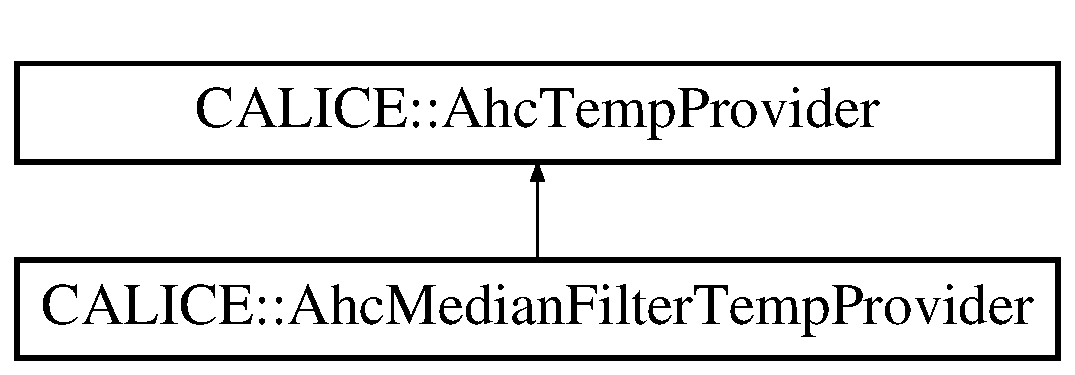
\includegraphics[height=2cm]{classCALICE_1_1AhcMedianFilterTempProvider}
\end{center}
\end{figure}
\subsection*{Public Member Functions}
\begin{DoxyCompactItemize}
\item 
{\bfseries AhcMedianFilterTempProvider} ({\bf AhcMapper} const $\ast$mapper)\label{classCALICE_1_1AhcMedianFilterTempProvider_afc6895b4468f12307c2da9f64c3eb5ed}

\item 
virtual float {\bf getCellTemp} (int module, int chip, int chan)
\begin{DoxyCompactList}\small\item\em Returns the temperature for the cell in the specified module connected to the given chip and channel. \item\end{DoxyCompactList}\item 
virtual float {\bf getCellTempError} (int module, int chip, int chan)\label{classCALICE_1_1AhcMedianFilterTempProvider_ace083f026078087a40383dd051d34843}

\begin{DoxyCompactList}\small\item\em Returns the error on the temperature for the cell in the specified module connected to the given chip and channel. \item\end{DoxyCompactList}\item 
virtual float {\bf getAvgTemp} ()\label{classCALICE_1_1AhcMedianFilterTempProvider_a237fba51962e5102c9580cfa9ed431fa}

\begin{DoxyCompactList}\small\item\em Returns the average calorimeter temperature. \item\end{DoxyCompactList}\item 
virtual float {\bf getAvgModuleTemp} (unsigned module)\label{classCALICE_1_1AhcMedianFilterTempProvider_a5395b7d6095c39af7e0b80b133ba400d}

\begin{DoxyCompactList}\small\item\em Returns the average module temperature. \item\end{DoxyCompactList}\item 
float {\bf getSensorTemp} (int module, int sensor)\label{classCALICE_1_1AhcMedianFilterTempProvider_ac9f730849a87bda3106773b7dc869f2e}

\begin{DoxyCompactList}\small\item\em Return the temperature for the specified module and sensor. \item\end{DoxyCompactList}\end{DoxyCompactItemize}
\subsection*{Protected Member Functions}
\begin{DoxyCompactItemize}
\item 
virtual void {\bf applyCorrection} ()
\begin{DoxyCompactList}\small\item\em This function applies the correction to the internal 'cache' for the temperature values from the five sensors. \item\end{DoxyCompactList}\item 
bool {\bf isBadValue} (float t)\label{classCALICE_1_1AhcMedianFilterTempProvider_a708c84d516d63059ba6665dae2da147e}

\begin{DoxyCompactList}\small\item\em Returns true if argument value is outside the sanity range. \item\end{DoxyCompactList}\end{DoxyCompactItemize}
\subsection*{Private Member Functions}
\begin{DoxyCompactItemize}
\item 
int {\bf getSensor} (int chip, int chan)\label{classCALICE_1_1AhcMedianFilterTempProvider_a23a23ba36d563be88a3f1a20a51b28c9}

\begin{DoxyCompactList}\small\item\em Returns the closest sensor to cell connected to chip, chan according to DESY-\/THESIS-\/2008-\/050. \item\end{DoxyCompactList}\item 
double {\bfseries median} (float a[$\,$], int n)\label{classCALICE_1_1AhcMedianFilterTempProvider_acab9513cd7e4395371bde8d433177cdb}

\end{DoxyCompactItemize}
\subsection*{Private Attributes}
\begin{DoxyCompactItemize}
\item 
{\bf AhcMapper} const $\ast$ {\bfseries \_\-mapper}\label{classCALICE_1_1AhcMedianFilterTempProvider_aa401791e44b7cc8c0c9093b66d84ac6a}

\item 
float {\bfseries \_\-caloMeanTemp}\label{classCALICE_1_1AhcMedianFilterTempProvider_a76bfbd1b9fd6deead5eeaf572f2498ef}

\item 
float {\bfseries \_\-caloMeanTempRMS}\label{classCALICE_1_1AhcMedianFilterTempProvider_a73f567416a0bcb8b5f8a130df8cad1f3}

\item 
int {\bfseries \_\-caloMeanCount}\label{classCALICE_1_1AhcMedianFilterTempProvider_abfa3e2672c774bc6814b5f44eda6ba9a}

\item 
std::vector$<$ float $>$ {\bfseries \_\-moduleMeanTemp}\label{classCALICE_1_1AhcMedianFilterTempProvider_a20f5463fcf3ba997a6b081615830940f}

\item 
std::vector$<$ float $>$ {\bfseries \_\-moduleMeanTempRMS}\label{classCALICE_1_1AhcMedianFilterTempProvider_aecb3f33637742eb7af6b9e0cbdb276a8}

\item 
std::vector$<$ int $>$ {\bfseries \_\-moduleMeanCount}\label{classCALICE_1_1AhcMedianFilterTempProvider_a17ece36832271a1590d721aabc0ce7ed}

\end{DoxyCompactItemize}


\subsection{Detailed Description}
This is a very simple temperature provider for the ahcal. What it does:
\begin{DoxyItemize}
\item the calibration set is applied
\item if a temperature sensor gives a value outside the defined sanity range the value is replaced by the average of the four sensors in that module
\item for each cell the temperature value from the 'closest' sensor, according to the table 3.1, DESY-\/THESIS-\/2008-\/050 is returned
\end{DoxyItemize}

Also see the documentation for the several functions for more detailed information. This new temperature provider with median filter created: Date: August 2013 Author: Sergey Morozov The temperature provider is based on the \doxyref{AhcSimpleTempProvider}{p.}{classCALICE_1_1AhcSimpleTempProvider} with some updates:
\begin{DoxyItemize}
\item all temperature sensors are set to the layer average temperature.
\item the median filter to layer-\/by-\/layer profile has been introduced. This will help to remove the out-\/layers with wrong temperature measurements in some layers of AHCAL. Note: you need smooth (median filtered for example) MIP and gain temperature profiles in the MIP and gain calibrations to use this tempetarure provider for data reconstruction! 
\end{DoxyItemize}

Definition at line 38 of file AhcMedianFilterTempProvider.hh.

\subsection{Member Function Documentation}
\index{CALICE::AhcMedianFilterTempProvider@{CALICE::AhcMedianFilterTempProvider}!applyCorrection@{applyCorrection}}
\index{applyCorrection@{applyCorrection}!CALICE::AhcMedianFilterTempProvider@{CALICE::AhcMedianFilterTempProvider}}
\subsubsection[{applyCorrection}]{\setlength{\rightskip}{0pt plus 5cm}void CALICE::AhcMedianFilterTempProvider::applyCorrection ()\hspace{0.3cm}{\ttfamily  [protected, virtual]}}\label{classCALICE_1_1AhcMedianFilterTempProvider_a9ffdad9db5836b0ceb55f317095cfe8c}


This function applies the correction to the internal 'cache' for the temperature values from the five sensors. It should be called everytime a new collection of temperatures or calibrations have been at set or the sanity range has been changed, i.e. if one of newSroModCol, newCalibCol or newSanityRange is true. This is done in \doxyref{getCellTemp()}{p.}{classCALICE_1_1AhcMedianFilterTempProvider_a2d5865711d94a975e593df2713608880} and \doxyref{getCellTempError()}{p.}{classCALICE_1_1AhcMedianFilterTempProvider_ace083f026078087a40383dd051d34843}. 

Definition at line 97 of file AhcMedianFilterTempProvider.cc.

References CALICE::AhcTempProvider::\_\-sroModCol, CALICE::AhcMapper::getK(), isBadValue(), CALICE::AhcTempProvider::newCalibCol, CALICE::AhcTempProvider::newSanityRange, CALICE::AhcTempProvider::newSroModCol, CALICE::AhcTempProvider::sensorTemp, CALICE::AhcTempProvider::sensorTempError, and CALICE::AhcTempProvider::updateCache().

Referenced by getAvgModuleTemp(), getAvgTemp(), getCellTemp(), getCellTempError(), and getSensorTemp().\index{CALICE::AhcMedianFilterTempProvider@{CALICE::AhcMedianFilterTempProvider}!getCellTemp@{getCellTemp}}
\index{getCellTemp@{getCellTemp}!CALICE::AhcMedianFilterTempProvider@{CALICE::AhcMedianFilterTempProvider}}
\subsubsection[{getCellTemp}]{\setlength{\rightskip}{0pt plus 5cm}float CALICE::AhcMedianFilterTempProvider::getCellTemp (int {\em module}, \/  int {\em chip}, \/  int {\em chan})\hspace{0.3cm}{\ttfamily  [virtual]}}\label{classCALICE_1_1AhcMedianFilterTempProvider_a2d5865711d94a975e593df2713608880}


Returns the temperature for the cell in the specified module connected to the given chip and channel. For each cell the temperature value from the 'closest' sensor, according to the table 3.1, DESY-\/THESIS-\/2008-\/050 is returned. 

Implements {\bf CALICE::AhcTempProvider} \doxyref{}{p.}{classCALICE_1_1AhcTempProvider_aa12c75d45d7ade54316dd113a6bab2d1}.

Definition at line 19 of file AhcMedianFilterTempProvider.cc.

References applyCorrection(), getSensor(), CALICE::AhcTempProvider::newCalibCol, CALICE::AhcTempProvider::newSanityRange, CALICE::AhcTempProvider::newSroModCol, and CALICE::AhcTempProvider::sensorTemp.

The documentation for this class was generated from the following files:\begin{DoxyCompactItemize}
\item 
AhcMedianFilterTempProvider.hh\item 
AhcMedianFilterTempProvider.cc\end{DoxyCompactItemize}

\section{CALICE::AhcSimpleTempProvider Class Reference}
\label{classCALICE_1_1AhcSimpleTempProvider}\index{CALICE::AhcSimpleTempProvider@{CALICE::AhcSimpleTempProvider}}


This is a very simple temperature provider for the ahcal.  


{\ttfamily \#include $<$AhcSimpleTempProvider.hh$>$}Inheritance diagram for CALICE::AhcSimpleTempProvider::\begin{figure}[H]
\begin{center}
\leavevmode
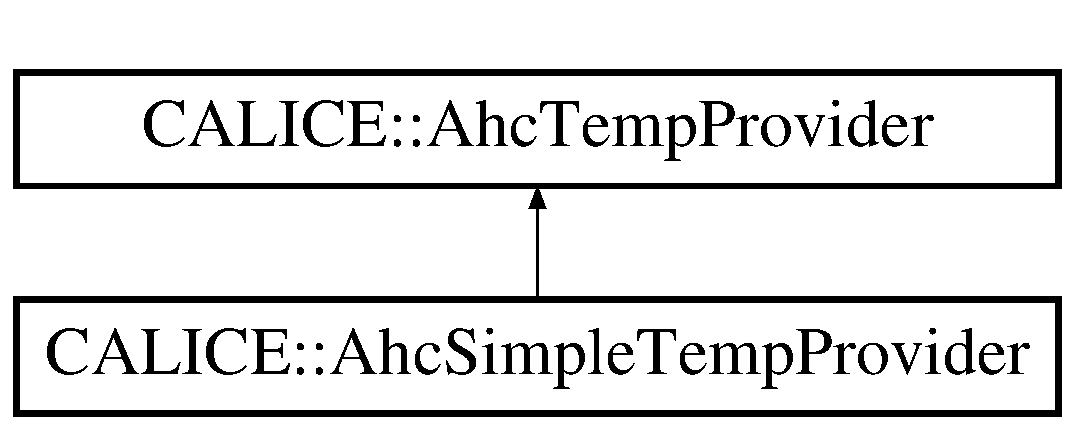
\includegraphics[height=2cm]{classCALICE_1_1AhcSimpleTempProvider}
\end{center}
\end{figure}
\subsection*{Public Member Functions}
\begin{DoxyCompactItemize}
\item 
virtual float {\bf getCellTemp} (int module, int chip, int chan)
\begin{DoxyCompactList}\small\item\em Returns the temperature for the cell in the specified module connected to the given chip and channel. \item\end{DoxyCompactList}\item 
virtual float {\bf getCellTempError} (int module, int chip, int chan)\label{classCALICE_1_1AhcSimpleTempProvider_a2d3cd7fd1a3f144f62991e39b44d016f}

\begin{DoxyCompactList}\small\item\em Returns the error on the temperature for the cell in the specified module connected to the given chip and channel. \item\end{DoxyCompactList}\item 
virtual float {\bf getAvgTemp} ()\label{classCALICE_1_1AhcSimpleTempProvider_ae2055a46cab875cb672f33bf6395b3b7}

\begin{DoxyCompactList}\small\item\em Returns the average calorimeter temperature. \item\end{DoxyCompactList}\item 
virtual float {\bf getAvgModuleTemp} (unsigned module)\label{classCALICE_1_1AhcSimpleTempProvider_abff6b07a15d952dc1f90a6e41500dabc}

\begin{DoxyCompactList}\small\item\em Returns the average module temperature. \item\end{DoxyCompactList}\item 
float {\bf getSensorTemp} (int module, int sensor)\label{classCALICE_1_1AhcSimpleTempProvider_ab61d13863930498a336476d9ac049b2e}

\begin{DoxyCompactList}\small\item\em Return the temperature for the specified module and sensor. \item\end{DoxyCompactList}\end{DoxyCompactItemize}
\subsection*{Protected Member Functions}
\begin{DoxyCompactItemize}
\item 
virtual void {\bf applyCorrection} ()
\begin{DoxyCompactList}\small\item\em This function applies the correction to the internal 'cache' for the temperature values from the five sensors. \item\end{DoxyCompactList}\item 
bool {\bf isBadValue} (float t)\label{classCALICE_1_1AhcSimpleTempProvider_ab3f94a954ed71d269997f0b2cde87941}

\begin{DoxyCompactList}\small\item\em Returns true if argument value is outside the sanity range. \item\end{DoxyCompactList}\end{DoxyCompactItemize}
\subsection*{Private Member Functions}
\begin{DoxyCompactItemize}
\item 
int {\bf getSensor} (int chip, int chan)\label{classCALICE_1_1AhcSimpleTempProvider_ad000dcb24a383043a9c72b93d2f05836}

\begin{DoxyCompactList}\small\item\em Returns the closest sensor to cell connected to chip, chan according to DESY-\/THESIS-\/2008-\/050. \item\end{DoxyCompactList}\end{DoxyCompactItemize}
\subsection*{Private Attributes}
\begin{DoxyCompactItemize}
\item 
float {\bfseries \_\-caloMeanTemp}\label{classCALICE_1_1AhcSimpleTempProvider_a254fa40b19cdc8b1c09a04b201afff2f}

\item 
float {\bfseries \_\-caloMeanTempRMS}\label{classCALICE_1_1AhcSimpleTempProvider_abe15d788019a2a354f8060dbfb9ef6e3}

\item 
int {\bfseries \_\-caloMeanCount}\label{classCALICE_1_1AhcSimpleTempProvider_a25cd84b21c382d4b7a2fc377588244b9}

\item 
std::vector$<$ float $>$ {\bfseries \_\-moduleMeanTemp}\label{classCALICE_1_1AhcSimpleTempProvider_a4d9109bd33c31ae2b06497ff73aeeb6e}

\item 
std::vector$<$ float $>$ {\bfseries \_\-moduleMeanTempRMS}\label{classCALICE_1_1AhcSimpleTempProvider_a7573f43d01d8a5563367f15527ed711e}

\item 
std::vector$<$ int $>$ {\bfseries \_\-moduleMeanCount}\label{classCALICE_1_1AhcSimpleTempProvider_ad3c12b5824a629e59d8dcc4ff4869684}

\end{DoxyCompactItemize}


\subsection{Detailed Description}
This is a very simple temperature provider for the ahcal. What it does:
\begin{DoxyItemize}
\item the calibration set is applied
\item if a temperature sensor gives a value outside the defined sanity range the value is replaced by the average of the four sensors in that module
\item for each cell the temperature value from the 'closest' sensor, according to the table 3.1, DESY-\/THESIS-\/2008-\/050 is returned
\end{DoxyItemize}

Also see the documentation for the several functions for more detailed information. 

Definition at line 25 of file AhcSimpleTempProvider.hh.

\subsection{Member Function Documentation}
\index{CALICE::AhcSimpleTempProvider@{CALICE::AhcSimpleTempProvider}!applyCorrection@{applyCorrection}}
\index{applyCorrection@{applyCorrection}!CALICE::AhcSimpleTempProvider@{CALICE::AhcSimpleTempProvider}}
\subsubsection[{applyCorrection}]{\setlength{\rightskip}{0pt plus 5cm}void CALICE::AhcSimpleTempProvider::applyCorrection ()\hspace{0.3cm}{\ttfamily  [protected, virtual]}}\label{classCALICE_1_1AhcSimpleTempProvider_a465f433cd5082a1c3224262e179604e1}


This function applies the correction to the internal 'cache' for the temperature values from the five sensors. It should be called everytime a new collection of temperatures or calibrations have been at set or the sanity range has been changed, i.e. if one of newSroModCol, newCalibCol or newSanityRange is true. This is done in \doxyref{getCellTemp()}{p.}{classCALICE_1_1AhcSimpleTempProvider_aff9186dfdab4801e41540f1d63428e3f} and \doxyref{getCellTempError()}{p.}{classCALICE_1_1AhcSimpleTempProvider_a2d3cd7fd1a3f144f62991e39b44d016f}. 

Definition at line 82 of file AhcSimpleTempProvider.cc.

References CALICE::AhcTempProvider::\_\-sroModCol, isBadValue(), CALICE::AhcTempProvider::newCalibCol, CALICE::AhcTempProvider::newSanityRange, CALICE::AhcTempProvider::newSroModCol, CALICE::AhcTempProvider::sensorTemp, CALICE::AhcTempProvider::sensorTempError, and CALICE::AhcTempProvider::updateCache().

Referenced by getAvgModuleTemp(), getAvgTemp(), getCellTemp(), getCellTempError(), and getSensorTemp().\index{CALICE::AhcSimpleTempProvider@{CALICE::AhcSimpleTempProvider}!getCellTemp@{getCellTemp}}
\index{getCellTemp@{getCellTemp}!CALICE::AhcSimpleTempProvider@{CALICE::AhcSimpleTempProvider}}
\subsubsection[{getCellTemp}]{\setlength{\rightskip}{0pt plus 5cm}float CALICE::AhcSimpleTempProvider::getCellTemp (int {\em module}, \/  int {\em chip}, \/  int {\em chan})\hspace{0.3cm}{\ttfamily  [virtual]}}\label{classCALICE_1_1AhcSimpleTempProvider_aff9186dfdab4801e41540f1d63428e3f}


Returns the temperature for the cell in the specified module connected to the given chip and channel. For each cell the temperature value from the 'closest' sensor, according to the table 3.1, DESY-\/THESIS-\/2008-\/050 is returned. 

Implements {\bf CALICE::AhcTempProvider} \doxyref{}{p.}{classCALICE_1_1AhcTempProvider_aa12c75d45d7ade54316dd113a6bab2d1}.

Definition at line 6 of file AhcSimpleTempProvider.cc.

References applyCorrection(), getSensor(), CALICE::AhcTempProvider::newCalibCol, CALICE::AhcTempProvider::newSanityRange, CALICE::AhcTempProvider::newSroModCol, and CALICE::AhcTempProvider::sensorTemp.

The documentation for this class was generated from the following files:\begin{DoxyCompactItemize}
\item 
AhcSimpleTempProvider.hh\item 
AhcSimpleTempProvider.cc\end{DoxyCompactItemize}

\section{CALICE::AhcSlowReadoutBlock Class Reference}
\label{classCALICE_1_1AhcSlowReadoutBlock}\index{CALICE::AhcSlowReadoutBlock@{CALICE::AhcSlowReadoutBlock}}


Interface Class to access the AhcSlowConfiguration Data For the time being we treat only the movable stage positions Update: 6/7/08 Added z and rotated position of stage (Maintain backward compatibility).  


{\ttfamily \#include $<$AhcSlowReadoutBlock.hh$>$}Inheritance diagram for CALICE::AhcSlowReadoutBlock::\begin{figure}[H]
\begin{center}
\leavevmode
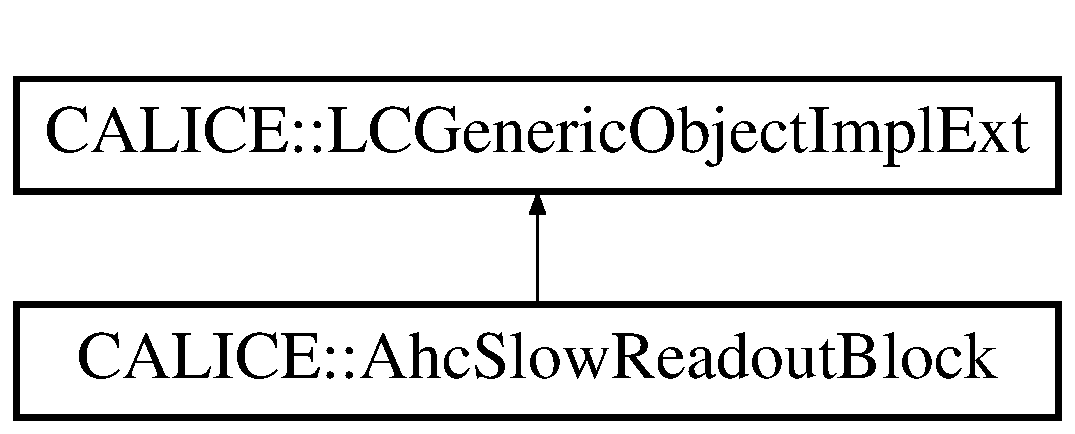
\includegraphics[height=2cm]{classCALICE_1_1AhcSlowReadoutBlock}
\end{center}
\end{figure}
\subsection*{Public Member Functions}
\begin{DoxyCompactItemize}
\item 
{\bf AhcSlowReadoutBlock} ()\label{classCALICE_1_1AhcSlowReadoutBlock_a5cdefa13a9db415369ef3df6e3b39da8}

\begin{DoxyCompactList}\small\item\em Simple Constructor. \item\end{DoxyCompactList}\item 
{\bf AhcSlowReadoutBlock} (LCObject $\ast$obj)\label{classCALICE_1_1AhcSlowReadoutBlock_a5b753db9f7e51e90eb67ca16e053faac}

\begin{DoxyCompactList}\small\item\em 'Copy constructor' needed to interpret LCCollection read from file/database. \item\end{DoxyCompactList}\item 
{\bf AhcSlowReadoutBlock} \& {\bfseries set\_\-xyzPosition\_\-mm} (double xpos, double ypos, double zpos)\label{classCALICE_1_1AhcSlowReadoutBlock_a07a5a75c46e30d25d87c46d5cf8dba73}

\item 
{\bf AhcSlowReadoutBlock} \& {\bfseries set\_\-rotPosition\_\-deg} (double cpos)\label{classCALICE_1_1AhcSlowReadoutBlock_aa4a13bec9f6c5db71c8cf3b793c08709}

\item 
virtual double {\bfseries get\_\-xPosition\_\-mm} ()\label{classCALICE_1_1AhcSlowReadoutBlock_a62d5383dfd433dc6eebbd38abd1f8a7c}

\item 
virtual double {\bfseries get\_\-yPosition\_\-mm} ()\label{classCALICE_1_1AhcSlowReadoutBlock_a59c904fd485befa6d9afe0cd2424ab20}

\item 
virtual double {\bfseries get\_\-zPosition\_\-mm} ()\label{classCALICE_1_1AhcSlowReadoutBlock_a73203222645101c2b8ce65736bf7752f}

\item 
virtual double {\bfseries get\_\-cPosition\_\-deg} ()\label{classCALICE_1_1AhcSlowReadoutBlock_add5f7179047770f32f533ac660612b1d}

\item 
void {\bf print} (std::ostream \&os)\label{classCALICE_1_1AhcSlowReadoutBlock_a4133b32c50c5946b39da0f961811f09a}

\begin{DoxyCompactList}\small\item\em Convenient print method. \item\end{DoxyCompactList}\item 
const std::string {\bf getTypeName} () const \label{classCALICE_1_1AhcSlowReadoutBlock_ae8699367e40866501f179e740a80bcab}

\begin{DoxyCompactList}\small\item\em Return the type of the class. \item\end{DoxyCompactList}\item 
const std::string {\bf getDataDescription} () const \label{classCALICE_1_1AhcSlowReadoutBlock_ae057949d71e0d6d7f4f2a808222b683c}

\begin{DoxyCompactList}\small\item\em Return a brief description of the data members. \item\end{DoxyCompactList}\end{DoxyCompactItemize}


\subsection{Detailed Description}
Interface Class to access the AhcSlowConfiguration Data For the time being we treat only the movable stage positions Update: 6/7/08 Added z and rotated position of stage (Maintain backward compatibility). \begin{DoxyAuthor}{Author}
: Roman P�schl DESY 
\end{DoxyAuthor}
\begin{DoxyDate}{Date}
Nov 2005 
\end{DoxyDate}


Definition at line 28 of file AhcSlowReadoutBlock.hh.

The documentation for this class was generated from the following files:\begin{DoxyCompactItemize}
\item 
AhcSlowReadoutBlock.hh\item 
AhcSlowReadoutBlock.cc\end{DoxyCompactItemize}

\section{CALICE::AhcSlowReadoutModBlock Class Reference}
\label{classCALICE_1_1AhcSlowReadoutModBlock}\index{CALICE::AhcSlowReadoutModBlock@{CALICE::AhcSlowReadoutModBlock}}


Interface Class to access the AhcSlowReadout Data Here we handle ahc voltages, temperatures et al.  


{\ttfamily \#include $<$AhcSlowReadoutModBlock.hh$>$}Inheritance diagram for CALICE::AhcSlowReadoutModBlock::\begin{figure}[H]
\begin{center}
\leavevmode
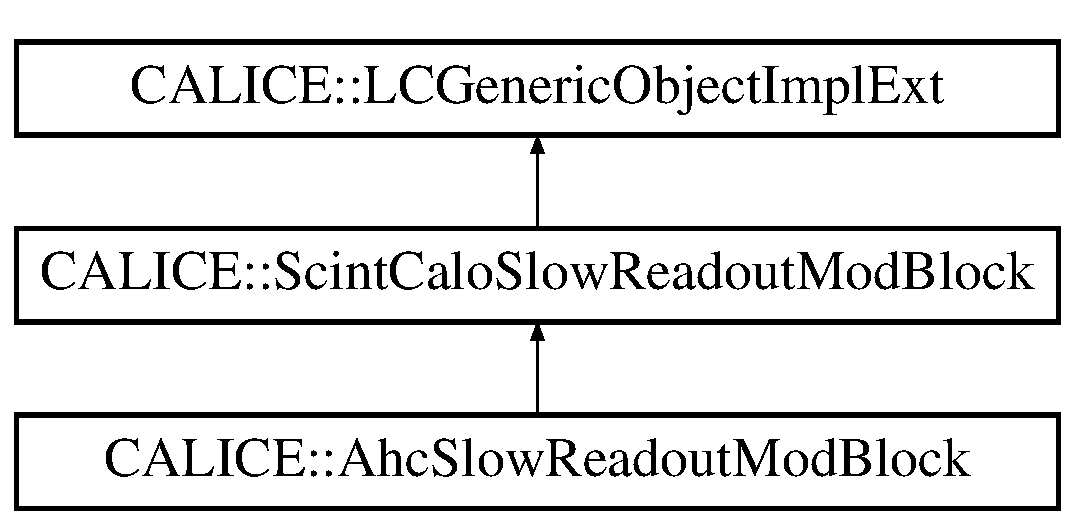
\includegraphics[height=3cm]{classCALICE_1_1AhcSlowReadoutModBlock}
\end{center}
\end{figure}
\subsection*{Public Member Functions}
\begin{DoxyCompactItemize}
\item 
{\bf AhcSlowReadoutModBlock} ()\label{classCALICE_1_1AhcSlowReadoutModBlock_a78919030cda78f1b40731c8124a28eac}

\begin{DoxyCompactList}\small\item\em Constructor. \item\end{DoxyCompactList}\item 
{\bf AhcSlowReadoutModBlock} (LCObject $\ast$obj)\label{classCALICE_1_1AhcSlowReadoutModBlock_a9a979a604c82e966f9a30ae3b55971ac}

\begin{DoxyCompactList}\small\item\em 'Copy constructor' needed to interpret LCCollection read from file/database. \item\end{DoxyCompactList}\item 
std::vector$<$ double $>$ \& {\bf getCmbValues} ()\label{classCALICE_1_1AhcSlowReadoutModBlock_aac2c55bb18e8ca946d12c227de07d9a7}

\begin{DoxyCompactList}\small\item\em Retrieve the cmb values. \item\end{DoxyCompactList}\item 
std::vector$<$ double $>$ \& {\bf getHbabTemperatures} ()\label{classCALICE_1_1AhcSlowReadoutModBlock_aad610827ad3485169aa9706cbc7128bb}

\begin{DoxyCompactList}\small\item\em Retrieve the hbab temperatures. \item\end{DoxyCompactList}\item 
void {\bf print} (std::ostream \&)
\begin{DoxyCompactList}\small\item\em convenient print method \item\end{DoxyCompactList}\item 
virtual const std::string {\bf getTypeName} () const \label{classCALICE_1_1AhcSlowReadoutModBlock_a0dc8e7472edb78736a8d740dab998e23}

\begin{DoxyCompactList}\small\item\em Return the type of the class. \item\end{DoxyCompactList}\item 
virtual const std::string {\bf getDataDescription} () const \label{classCALICE_1_1AhcSlowReadoutModBlock_a8343c0f0c11517815ec3c9279cb63000}

\begin{DoxyCompactList}\small\item\em Return a brief description of the data members. \item\end{DoxyCompactList}\end{DoxyCompactItemize}
\subsection*{Private Member Functions}
\begin{DoxyCompactItemize}
\item 
void {\bf setTypes} ()\label{classCALICE_1_1AhcSlowReadoutModBlock_a4b22eb001e649f486a88bfddb2c1ed68}

\begin{DoxyCompactList}\small\item\em This method defines the (general) types of the measured values A type not present here will not be handled!!! \item\end{DoxyCompactList}\end{DoxyCompactItemize}
\subsection*{Private Attributes}
\begin{DoxyCompactItemize}
\item 
std::vector$<$ double $>$ {\bf \_\-cmbValues}
\begin{DoxyCompactList}\small\item\em The output vectors. \item\end{DoxyCompactList}\item 
std::vector$<$ double $>$ {\bf \_\-hbabTemperatures}\label{classCALICE_1_1AhcSlowReadoutModBlock_aedce23ae2abcf8741fd34ecc5d7a7e60}

\begin{DoxyCompactList}\small\item\em hbab temperatures \item\end{DoxyCompactList}\end{DoxyCompactItemize}


\subsection{Detailed Description}
Interface Class to access the AhcSlowReadout Data Here we handle ahc voltages, temperatures et al. when filling the class the string identifying the measured values has to be given first, a warning is issued if no identifier is given for a given datatype. On the other hand this concerns just the filler of the class, i.e. the conversion where it is done once for all. See the print method at the end of the class for the meaning of the fields (as of 31/7/06) Use the interface methods to retrieve the data fields \begin{DoxyAuthor}{Author}
Roman P�schl LAL/Orsay 
\end{DoxyAuthor}
\begin{DoxyDate}{Date}
Aug 2006 
\end{DoxyDate}


Definition at line 56 of file AhcSlowReadoutModBlock.hh.

\subsection{Member Function Documentation}
\index{CALICE::AhcSlowReadoutModBlock@{CALICE::AhcSlowReadoutModBlock}!print@{print}}
\index{print@{print}!CALICE::AhcSlowReadoutModBlock@{CALICE::AhcSlowReadoutModBlock}}
\subsubsection[{print}]{\setlength{\rightskip}{0pt plus 5cm}void CALICE::AhcSlowReadoutModBlock::print (std::ostream \& {\em os})}\label{classCALICE_1_1AhcSlowReadoutModBlock_a697eeaf3c34576c3c4541bdc3fcd35c2}


convenient print method Convenient print method. 

Reimplemented from {\bf CALICE::ScintCaloSlowReadoutModBlock} \doxyref{}{p.}{classCALICE_1_1ScintCaloSlowReadoutModBlock_af128d26796f6a009d9c0777947c7d050}.

Definition at line 33 of file AhcSlowReadoutModBlock.cc.

References CALICE::ScintCaloSlowReadoutModBlock::\_\-hbabVoltages, CALICE::ScintCaloSlowReadoutModBlock::getCmbHeight(), CALICE::ScintCaloSlowReadoutModBlock::getCmbTemperatures(), getCmbValues(), CALICE::ScintCaloSlowReadoutModBlock::getCmbVoltages(), CALICE::ScintCaloSlowReadoutModBlock::getCmbWidth(), getHbabTemperatures(), CALICE::ScintCaloSlowReadoutModBlock::getHbabVoltages(), CALICE::ScintCaloSlowReadoutModBlock::getLedSetting(), CALICE::ScintCaloSlowReadoutModBlock::getModuleNumber(), CALICE::ScintCaloSlowReadoutModBlock::getTimeStamp(), CALICE::ScintCaloSlowReadoutModBlock::prepareOutputVecs(), and CALICE::to\_\-binary\_\-bitops().

\subsection{Field Documentation}
\index{CALICE::AhcSlowReadoutModBlock@{CALICE::AhcSlowReadoutModBlock}!\_\-cmbValues@{\_\-cmbValues}}
\index{\_\-cmbValues@{\_\-cmbValues}!CALICE::AhcSlowReadoutModBlock@{CALICE::AhcSlowReadoutModBlock}}
\subsubsection[{\_\-cmbValues}]{\setlength{\rightskip}{0pt plus 5cm}std::vector$<$double$>$ {\bf CALICE::AhcSlowReadoutModBlock::\_\-cmbValues}\hspace{0.3cm}{\ttfamily  [private]}}\label{classCALICE_1_1AhcSlowReadoutModBlock_a99517926e9ee2d071d74bfab855dfca8}


The output vectors. cmb values 

Definition at line 120 of file AhcSlowReadoutModBlock.hh.

Referenced by AhcSlowReadoutModBlock(), getCmbValues(), and setTypes().

The documentation for this class was generated from the following files:\begin{DoxyCompactItemize}
\item 
AhcSlowReadoutModBlock.hh\item 
AhcSlowReadoutModBlock.cc\end{DoxyCompactItemize}

\section{CALICE::AhcSlowReadoutModMapper Class Reference}
\label{classCALICE_1_1AhcSlowReadoutModMapper}\index{CALICE::AhcSlowReadoutModMapper@{CALICE::AhcSlowReadoutModMapper}}


Class to correct the mapping of AhcSlowReadoutModBlock-\/classes.  


{\ttfamily \#include $<$AhcSlowReadoutModMapper.hh$>$}\subsection*{Public Member Functions}
\begin{DoxyCompactItemize}
\item 
lcio::LCCollection $\ast$ {\bf mapCollection} (const lcio::LCCollection $\ast$const col) const 
\begin{DoxyCompactList}\small\item\em returns collection with corrected AhcSlowReadoutModBlock-\/elements for an unmapped collection of \doxyref{AhcSlowReadoutModBlock}{p.}{classCALICE_1_1AhcSlowReadoutModBlock} \item\end{DoxyCompactList}\item 
void {\bf updateMapping} (const lcio::LCCollection $\ast$const col)
\begin{DoxyCompactList}\small\item\em Function to update the mapping. \item\end{DoxyCompactList}\end{DoxyCompactItemize}
\subsection*{Private Member Functions}
\begin{DoxyCompactItemize}
\item 
void {\bfseries init} ()\label{classCALICE_1_1AhcSlowReadoutModMapper_acdefd374a029f03e44e43ae651bc16fb}

\item 
void {\bfseries ensureSize} (unsigned int i)\label{classCALICE_1_1AhcSlowReadoutModMapper_a840d2c17a25ecfe401031047dbdf00b8}

\item 
bool {\bfseries isAvailable} (int module)\label{classCALICE_1_1AhcSlowReadoutModMapper_a8e06c12f239c65287643281ef986473d}

\item 
void {\bfseries setValues} ({\bf AhcSlowReadoutModBlock} $\ast$output, const std::vector$<$ {\bf AhcSlowReadoutModBlock} $\ast$ $>$ \&input, unsigned int module) const \label{classCALICE_1_1AhcSlowReadoutModMapper_a7ed1bd5cad8c574ed031c2d7ecc680aa}

\end{DoxyCompactItemize}
\subsection*{Private Attributes}
\begin{DoxyCompactItemize}
\item 
std::vector$<$ bool $>$ {\bfseries \_\-isAvailable}\label{classCALICE_1_1AhcSlowReadoutModMapper_a9c7cdd3f7492a7dcf9ce358a41d4e3a7}

\item 
std::vector$<$ int $>$ {\bfseries \_\-CMBlabel}\label{classCALICE_1_1AhcSlowReadoutModMapper_ae8b8700496f48a1e9056ec4ddd92abe7}

\item 
std::vector$<$ int $>$ {\bfseries \_\-HVlabel}\label{classCALICE_1_1AhcSlowReadoutModMapper_a1ad249bcd18e4ced012b5269671810ae}

\item 
std::vector$<$ int $>$ {\bfseries \_\-LVlabel}\label{classCALICE_1_1AhcSlowReadoutModMapper_a168f8dcf17583bc6e49b671c7824fcf7}

\end{DoxyCompactItemize}


\subsection{Detailed Description}
Class to correct the mapping of AhcSlowReadoutModBlock-\/classes. The class \doxyref{AhcSlowReadoutModBlock}{p.}{classCALICE_1_1AhcSlowReadoutModBlock} containes the module number for which the records stands. Due to problems in the slow control in the years 2006 and 2007 the values from the different data sources have been written with wrong module number. Therefore, the single \doxyref{AhcSlowReadoutModBlock}{p.}{classCALICE_1_1AhcSlowReadoutModBlock} contains a collection of values from different modules. e.g. record with label \char`\"{}module = 17\char`\"{} contains CMB readings from module 23, HV readings from module 19 and corrupted LV readings

This class collects, as far as possible, the datas for the modules from the different records these ended up. If the mapping for one part is missing the values for this source will not be filled.

\begin{DoxySeeAlso}{See also}
\doxyref{AhcSlowReadoutModBlock}{p.}{classCALICE_1_1AhcSlowReadoutModBlock} 

\doxyref{AhcSlowReadoutModMapping}{p.}{classCALICE_1_1AhcSlowReadoutModMapping}
\end{DoxySeeAlso}
\begin{DoxyAuthor}{Author}
{\tt Benjamin.Lutz@desy.de} 
\end{DoxyAuthor}
\begin{DoxyDate}{Date}
Nov 2008 
\end{DoxyDate}
\begin{DoxyVersion}{Version}
1.0 
\end{DoxyVersion}


Definition at line 34 of file AhcSlowReadoutModMapper.hh.

\subsection{Member Function Documentation}
\index{CALICE::AhcSlowReadoutModMapper@{CALICE::AhcSlowReadoutModMapper}!mapCollection@{mapCollection}}
\index{mapCollection@{mapCollection}!CALICE::AhcSlowReadoutModMapper@{CALICE::AhcSlowReadoutModMapper}}
\subsubsection[{mapCollection}]{\setlength{\rightskip}{0pt plus 5cm}lcio::LCCollection $\ast$ CALICE::AhcSlowReadoutModMapper::mapCollection (const lcio::LCCollection $\ast$const  {\em col}) const}\label{classCALICE_1_1AhcSlowReadoutModMapper_aaf98120ee4080f6de37b5017ea6e4bb1}


returns collection with corrected AhcSlowReadoutModBlock-\/elements for an unmapped collection of \doxyref{AhcSlowReadoutModBlock}{p.}{classCALICE_1_1AhcSlowReadoutModBlock} 
\begin{DoxyExceptions}{Exceptions}
\item[{\em \doxyref{WrongDataFormatException}{p.}{classCALICE_1_1WrongDataFormatException}}]When the collection type is not LCGenericObjects or the collection parameter \char`\"{}TypeName\char`\"{} is not \char`\"{}AhcSlowReadoutModBlock\char`\"{} \end{DoxyExceptions}

\begin{DoxyParams}{Parameters}
\item[\mbox{$\leftarrow$} {\em col}]collection of \doxyref{AhcSlowReadoutModBlock}{p.}{classCALICE_1_1AhcSlowReadoutModBlock} \end{DoxyParams}
\begin{DoxyReturn}{Returns}
corrected collection of \doxyref{AhcSlowReadoutModBlock}{p.}{classCALICE_1_1AhcSlowReadoutModBlock} 
\end{DoxyReturn}
\begin{DoxySeeAlso}{See also}
\doxyref{WrongDataFormatException}{p.}{classCALICE_1_1WrongDataFormatException} 

\doxyref{AhcSlowReadoutModBlock}{p.}{classCALICE_1_1AhcSlowReadoutModBlock} 
\end{DoxySeeAlso}


Definition at line 88 of file AhcSlowReadoutModMapper.cc.

References CALICE::ScintCaloSlowReadoutModBlock::getModuleNumber(), and CALICE::ScintCaloSlowReadoutModBlock::setModuleNumber().\index{CALICE::AhcSlowReadoutModMapper@{CALICE::AhcSlowReadoutModMapper}!updateMapping@{updateMapping}}
\index{updateMapping@{updateMapping}!CALICE::AhcSlowReadoutModMapper@{CALICE::AhcSlowReadoutModMapper}}
\subsubsection[{updateMapping}]{\setlength{\rightskip}{0pt plus 5cm}void CALICE::AhcSlowReadoutModMapper::updateMapping (const lcio::LCCollection $\ast$const  {\em col})}\label{classCALICE_1_1AhcSlowReadoutModMapper_a5e8636113c362bb680cf97ab0a63a9f6}


Function to update the mapping. 
\begin{DoxyExceptions}{Exceptions}
\item[{\em \doxyref{CALICE::WrongDataFormatException}{p.}{classCALICE_1_1WrongDataFormatException}}]When the collection type is not LCGenericObjects or the collection parameter \char`\"{}TypeName\char`\"{} is not \char`\"{}AhcSlowReadoutModMapping\char`\"{} \end{DoxyExceptions}

\begin{DoxyParams}{Parameters}
\item[\mbox{$\leftarrow$} {\em col}]The collection of \doxyref{AhcSlowReadoutModMapping}{p.}{classCALICE_1_1AhcSlowReadoutModMapping} objects \end{DoxyParams}
\begin{DoxySeeAlso}{See also}
\doxyref{WrongDataFormatException}{p.}{classCALICE_1_1WrongDataFormatException} 

\doxyref{AhcSlowReadoutModMapping}{p.}{classCALICE_1_1AhcSlowReadoutModMapping} 
\end{DoxySeeAlso}


Definition at line 133 of file AhcSlowReadoutModMapper.cc.

References CALICE::AhcSlowReadoutModMapping::getCMBlabel(), CALICE::AhcSlowReadoutModMapping::getHVlabel(), CALICE::AhcSlowReadoutModMapping::getLVlabel(), and CALICE::AhcSlowReadoutModMapping::getModule().

The documentation for this class was generated from the following files:\begin{DoxyCompactItemize}
\item 
AhcSlowReadoutModMapper.hh\item 
AhcSlowReadoutModMapper.cc\end{DoxyCompactItemize}

\section{CALICE::AhcSlowReadoutModMapping Class Reference}
\label{classCALICE_1_1AhcSlowReadoutModMapping}\index{CALICE::AhcSlowReadoutModMapping@{CALICE::AhcSlowReadoutModMapping}}


Class to store the mapping corrections for the \doxyref{AhcSlowReadoutModBlock}{p.}{classCALICE_1_1AhcSlowReadoutModBlock}.  


{\ttfamily \#include $<$AhcSlowReadoutModMapping.hh$>$}\subsection*{Public Member Functions}
\begin{DoxyCompactItemize}
\item 
{\bf AhcSlowReadoutModMapping} (const int module, const int CMBrecordLabel, const int HVrecordLabel, const int LVrecordLabel)\label{classCALICE_1_1AhcSlowReadoutModMapping_a04259684c066116f68e2f6e6cf95279d}

\begin{DoxyCompactList}\small\item\em Constructor with initial values. \item\end{DoxyCompactList}\item 
{\bf AhcSlowReadoutModMapping} (EVENT::LCObject $\ast$object)\label{classCALICE_1_1AhcSlowReadoutModMapping_a6739023171558d8ef871959a68d8236b}

\begin{DoxyCompactList}\small\item\em Constructor from LCObject. \item\end{DoxyCompactList}\item 
{\bf $\sim$AhcSlowReadoutModMapping} ()\label{classCALICE_1_1AhcSlowReadoutModMapping_a89417dbb3a023ddbb4a931d33b6d4ee7}

\begin{DoxyCompactList}\small\item\em Destructor. \item\end{DoxyCompactList}\item 
void {\bfseries setModule} (int module)\label{classCALICE_1_1AhcSlowReadoutModMapping_a1413edfe61deff586222939ba94bee02}

\item 
void {\bfseries setCMBlabel} (int label)\label{classCALICE_1_1AhcSlowReadoutModMapping_a27b72f9ef8901bde36ebc189e93ba0e1}

\item 
void {\bfseries setHVlabel} (int label)\label{classCALICE_1_1AhcSlowReadoutModMapping_af52b00986593fbc5be5cb989d1a1ab33}

\item 
void {\bfseries setLVlabel} (int label)\label{classCALICE_1_1AhcSlowReadoutModMapping_a50dde0c78870949667e71ce67532e6e5}

\item 
int {\bf getModule} () const \label{classCALICE_1_1AhcSlowReadoutModMapping_a835efcca7195eaedbf03c0b1801f2c9b}

\begin{DoxyCompactList}\small\item\em get the module number for which this record is \item\end{DoxyCompactList}\item 
int {\bf getCMBlabel} () const 
\begin{DoxyCompactList}\small\item\em get the label of the \doxyref{AhcSlowReadoutModBlock}{p.}{classCALICE_1_1AhcSlowReadoutModBlock} holding the data with source CMB \item\end{DoxyCompactList}\item 
int {\bf getHVlabel} () const 
\begin{DoxyCompactList}\small\item\em get the label of the \doxyref{AhcSlowReadoutModBlock}{p.}{classCALICE_1_1AhcSlowReadoutModBlock} holding the data with source HV supply \item\end{DoxyCompactList}\item 
int {\bf getLVlabel} () const 
\begin{DoxyCompactList}\small\item\em get the label of the \doxyref{AhcSlowReadoutModBlock}{p.}{classCALICE_1_1AhcSlowReadoutModBlock} holding the data with source LV monitoring \item\end{DoxyCompactList}\item 
const std::string {\bf getTypeName} () const \label{classCALICE_1_1AhcSlowReadoutModMapping_aeb86619ed81a290c41fcb00ce96489a9}

\begin{DoxyCompactList}\small\item\em Implementation of LCGenericObject::getTypeName. \item\end{DoxyCompactList}\item 
const std::string {\bf getDataDescription} () const \label{classCALICE_1_1AhcSlowReadoutModMapping_a52b2537a461e778f0b4c5e7e2b38218f}

\begin{DoxyCompactList}\small\item\em Implementation of LCGenericObject::getDataDescription. \item\end{DoxyCompactList}\end{DoxyCompactItemize}


\subsection{Detailed Description}
Class to store the mapping corrections for the \doxyref{AhcSlowReadoutModBlock}{p.}{classCALICE_1_1AhcSlowReadoutModBlock}. The slow control assembled the data from different modules into the slow control data submitted to the DAQ during 2006 and 2007. This bug was only fixed in the beginning of 2008 data taking at FNAL. This class holds the relation between data from the module and under which label it was stored.

As the data comes from three different hardware sources (CMB, HV supply and LV) the record holds three numbers for the sources. If the data for one source is lost due to mapping errors, the reading will be -\/1.

\begin{DoxyAuthor}{Author}
{\tt Benjamin.Lutz@desy.de} 
\end{DoxyAuthor}
\begin{DoxyVersion}{Version}
1.0 
\end{DoxyVersion}
\begin{DoxyDate}{Date}
November 2008 
\end{DoxyDate}


Definition at line 29 of file AhcSlowReadoutModMapping.hh.

\subsection{Member Function Documentation}
\index{CALICE::AhcSlowReadoutModMapping@{CALICE::AhcSlowReadoutModMapping}!getCMBlabel@{getCMBlabel}}
\index{getCMBlabel@{getCMBlabel}!CALICE::AhcSlowReadoutModMapping@{CALICE::AhcSlowReadoutModMapping}}
\subsubsection[{getCMBlabel}]{\setlength{\rightskip}{0pt plus 5cm}int CALICE::AhcSlowReadoutModMapping::getCMBlabel () const}\label{classCALICE_1_1AhcSlowReadoutModMapping_a39c6eca8f76b2b4fbfe7335f8fb79d9b}


get the label of the \doxyref{AhcSlowReadoutModBlock}{p.}{classCALICE_1_1AhcSlowReadoutModBlock} holding the data with source CMB \begin{DoxyRemark}{Remarks}
returns -\/1 when the data was lost due to mapping errors 
\end{DoxyRemark}


Definition at line 23 of file AhcSlowReadoutModMapping.cc.

Referenced by CALICE::AhcSlowReadoutModMapper::updateMapping().\index{CALICE::AhcSlowReadoutModMapping@{CALICE::AhcSlowReadoutModMapping}!getHVlabel@{getHVlabel}}
\index{getHVlabel@{getHVlabel}!CALICE::AhcSlowReadoutModMapping@{CALICE::AhcSlowReadoutModMapping}}
\subsubsection[{getHVlabel}]{\setlength{\rightskip}{0pt plus 5cm}int CALICE::AhcSlowReadoutModMapping::getHVlabel () const}\label{classCALICE_1_1AhcSlowReadoutModMapping_aff49b5b29efaabfb24466c01f1486661}


get the label of the \doxyref{AhcSlowReadoutModBlock}{p.}{classCALICE_1_1AhcSlowReadoutModBlock} holding the data with source HV supply \begin{DoxyRemark}{Remarks}
returns -\/1 when the data was lost due to mapping errors 
\end{DoxyRemark}


Definition at line 26 of file AhcSlowReadoutModMapping.cc.

Referenced by CALICE::AhcSlowReadoutModMapper::updateMapping().\index{CALICE::AhcSlowReadoutModMapping@{CALICE::AhcSlowReadoutModMapping}!getLVlabel@{getLVlabel}}
\index{getLVlabel@{getLVlabel}!CALICE::AhcSlowReadoutModMapping@{CALICE::AhcSlowReadoutModMapping}}
\subsubsection[{getLVlabel}]{\setlength{\rightskip}{0pt plus 5cm}int CALICE::AhcSlowReadoutModMapping::getLVlabel () const}\label{classCALICE_1_1AhcSlowReadoutModMapping_a68c0787c9d421cb85938ecc4e0ca1b27}


get the label of the \doxyref{AhcSlowReadoutModBlock}{p.}{classCALICE_1_1AhcSlowReadoutModBlock} holding the data with source LV monitoring \begin{DoxyRemark}{Remarks}
returns -\/1 when the data was lost due to mapping errors 
\end{DoxyRemark}


Definition at line 29 of file AhcSlowReadoutModMapping.cc.

Referenced by CALICE::AhcSlowReadoutModMapper::updateMapping().

The documentation for this class was generated from the following files:\begin{DoxyCompactItemize}
\item 
AhcSlowReadoutModMapping.hh\item 
AhcSlowReadoutModMapping.cc\end{DoxyCompactItemize}

\section{CALICE::AhcTempProvider Class Reference}
\label{classCALICE_1_1AhcTempProvider}\index{CALICE::AhcTempProvider@{CALICE::AhcTempProvider}}


This is an abstract class defining an interface to access the temperatures in single AHCAL cells.  


{\ttfamily \#include $<$AhcTempProvider.hh$>$}Inheritance diagram for CALICE::AhcTempProvider::\begin{figure}[H]
\begin{center}
\leavevmode
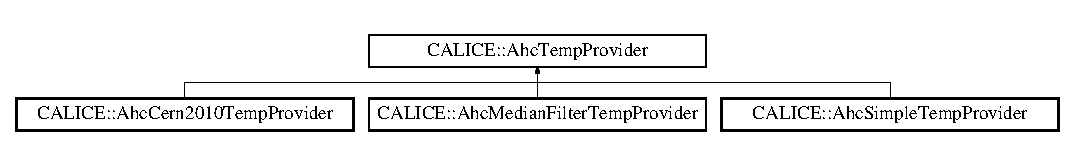
\includegraphics[height=1.53005cm]{classCALICE_1_1AhcTempProvider}
\end{center}
\end{figure}
\subsection*{Public Member Functions}
\begin{DoxyCompactItemize}
\item 
{\bf AhcTempProvider} ()\label{classCALICE_1_1AhcTempProvider_ab4f94c3219c7389ce3871daea4396b4a}

\begin{DoxyCompactList}\small\item\em Default constructor. \item\end{DoxyCompactList}\item 
virtual {\bf $\sim$AhcTempProvider} ()\label{classCALICE_1_1AhcTempProvider_a53d2786bdade2bbcbee773091e774947}

\begin{DoxyCompactList}\small\item\em Default destructor. \item\end{DoxyCompactList}\item 
virtual float {\bf getCellTemp} (int module, int chip, int chan)=0
\begin{DoxyCompactList}\small\item\em Returns the temperature for the cell in the specified module connected to the given chip and channel. \item\end{DoxyCompactList}\item 
virtual float {\bf getCellTempError} (int module, int chip, int chan)=0
\begin{DoxyCompactList}\small\item\em Returns the error on the temperature for the cell in the specified module connected to the given chip and channel. \item\end{DoxyCompactList}\item 
virtual void {\bf setAhcSroModBlocks} (lcio::LCCollection $\ast$col)\label{classCALICE_1_1AhcTempProvider_a938c5064c310531a44b5ba6905dc1705}

\begin{DoxyCompactList}\small\item\em Set the collection of \doxyref{AhcSlowReadoutModBlock}{p.}{classCALICE_1_1AhcSlowReadoutModBlock} objects to extract the temperature data from. \item\end{DoxyCompactList}\item 
virtual float {\bf getAvgTemp} ()=0\label{classCALICE_1_1AhcTempProvider_a69b50b787f49a84132c7a264516bcf1f}

\begin{DoxyCompactList}\small\item\em Returns the average calorimeter temperature. \item\end{DoxyCompactList}\item 
virtual float {\bf getAvgModuleTemp} (unsigned module)=0\label{classCALICE_1_1AhcTempProvider_a1d4cf73aa7a2308ef910247cc1612760}

\begin{DoxyCompactList}\small\item\em Returns the average module temperature. \item\end{DoxyCompactList}\item 
virtual float {\bf getSensorTemp} (int module, int sensor)=0
\begin{DoxyCompactList}\small\item\em Returns the temperature of the specified sensor in the given module. \item\end{DoxyCompactList}\item 
virtual void {\bf setCalibrations} (lcio::LCCollection $\ast$col)\label{classCALICE_1_1AhcTempProvider_a9d3babda133b664e703113bb7b47dbdd}

\begin{DoxyCompactList}\small\item\em Set the collection of \doxyref{SimpleValue}{p.}{classCALICE_1_1SimpleValue} objects to use for the offset calibrations of the temperature sensors. \item\end{DoxyCompactList}\item 
virtual void {\bf setSanityRange} (float min, float max)
\begin{DoxyCompactList}\small\item\em Define a sanity range of temperature values that make sense. \item\end{DoxyCompactList}\end{DoxyCompactItemize}
\subsection*{Static Public Attributes}
\begin{DoxyCompactItemize}
\item 
static const unsigned {\bfseries N\_\-MODULES} = 38\label{classCALICE_1_1AhcTempProvider_a2fb5517d9cf3179ccb581d37cc91097a}

\item 
static const unsigned {\bfseries N\_\-SENSORS} = 5\label{classCALICE_1_1AhcTempProvider_adfe5f33f2eeae2901e32edca4515cd20}

\end{DoxyCompactItemize}
\subsection*{Protected Member Functions}
\begin{DoxyCompactItemize}
\item 
virtual void {\bf updateCache} ()
\begin{DoxyCompactList}\small\item\em This function updates the internal 'cache' for the temperature values from the five sensors and applies the calibration offsets, if available. \item\end{DoxyCompactList}\end{DoxyCompactItemize}
\subsection*{Protected Attributes}
\begin{DoxyCompactItemize}
\item 
bool {\bf newSroModCol}
\begin{DoxyCompactList}\small\item\em If true this indicates that setSroModBlocks() was called and a new collection of AhcSroModBlock objects was set. \item\end{DoxyCompactList}\item 
bool {\bf newCalibCol}
\begin{DoxyCompactList}\small\item\em If true this indicates that \doxyref{setCalibrations()}{p.}{classCALICE_1_1AhcTempProvider_a9d3babda133b664e703113bb7b47dbdd} was called and a new collection of calibrations was set. \item\end{DoxyCompactList}\item 
bool {\bf newSanityRange}
\begin{DoxyCompactList}\small\item\em If true this indicates that \doxyref{setSanityRange()}{p.}{classCALICE_1_1AhcTempProvider_add95eab55a99250ec9f0666fc34ba40d} was called and a new sanity range was set. \item\end{DoxyCompactList}\item 
std::vector$<$ std::vector$<$ float $>$ $>$ {\bf sensorTemp}
\begin{DoxyCompactList}\small\item\em This is a 'cache' for the values of the temperature sensors after calibration and and correction. \item\end{DoxyCompactList}\item 
std::vector$<$ std::vector$<$ float $>$ $>$ {\bf sensorTempError}
\begin{DoxyCompactList}\small\item\em This is a 'cache' for the errors on the values of the temperature sensors after calibration and and correction. \item\end{DoxyCompactList}\item 
std::vector$<$ std::vector$<$ float $>$ $>$ {\bf sensorCalib}
\begin{DoxyCompactList}\small\item\em This is a 'cache' for the calibration offsets for the temperature sensors. \item\end{DoxyCompactList}\item 
std::vector$<$ std::vector$<$ float $>$ $>$ {\bf sensorCalibError}
\begin{DoxyCompactList}\small\item\em This is a 'cache' for the errors on the calibration offsets for the temperature sensors. \item\end{DoxyCompactList}\item 
std::vector$<$ std::vector$<$ int $>$ $>$ {\bf sensorCalibStatus}\label{classCALICE_1_1AhcTempProvider_af49e3cc723e4ce780660fe181fd2b40f}

\begin{DoxyCompactList}\small\item\em Vector to save the status of the calibration offsets. \item\end{DoxyCompactList}\item 
float {\bf \_\-sanityMin}\label{classCALICE_1_1AhcTempProvider_acdf8e26d39ac276e7eac53b2746348c2}

\begin{DoxyCompactList}\small\item\em Lower limit of the sanity range. \item\end{DoxyCompactList}\item 
float {\bf \_\-sanityMax}\label{classCALICE_1_1AhcTempProvider_a5c8919447ae0eece8b050ea21bc80e15}

\begin{DoxyCompactList}\small\item\em Upper limit of the sanity range. \item\end{DoxyCompactList}\item 
lcio::LCCollection $\ast$ {\bf \_\-sroModCol}\label{classCALICE_1_1AhcTempProvider_a6d03fdcfc0a4fedc590597f4383d36ae}

\begin{DoxyCompactList}\small\item\em A pointer to the LCCollection containing the AhcSlowReadOut objects. \item\end{DoxyCompactList}\item 
lcio::LCCollection $\ast$ {\bf \_\-calibCol}\label{classCALICE_1_1AhcTempProvider_aed886ffef7d22bdcfbfa4e00b6c27f9f}

\begin{DoxyCompactList}\small\item\em A pointer to the LCCollection containing the calibration offsets objects. \item\end{DoxyCompactList}\end{DoxyCompactItemize}


\subsection{Detailed Description}
This is an abstract class defining an interface to access the temperatures in single AHCAL cells. 

Definition at line 21 of file AhcTempProvider.hh.

\subsection{Member Function Documentation}
\index{CALICE::AhcTempProvider@{CALICE::AhcTempProvider}!getCellTemp@{getCellTemp}}
\index{getCellTemp@{getCellTemp}!CALICE::AhcTempProvider@{CALICE::AhcTempProvider}}
\subsubsection[{getCellTemp}]{\setlength{\rightskip}{0pt plus 5cm}virtual float CALICE::AhcTempProvider::getCellTemp (int {\em module}, \/  int {\em chip}, \/  int {\em chan})\hspace{0.3cm}{\ttfamily  [pure virtual]}}\label{classCALICE_1_1AhcTempProvider_aa12c75d45d7ade54316dd113a6bab2d1}


Returns the temperature for the cell in the specified module connected to the given chip and channel. This is only the definition of the interface, a concrete funtion has to be implemented in a derived class. Note: Modules are counted from 1! The valid range for module numbers thus is 1 to 38. 

Implemented in {\bf CALICE::AhcCern2010TempProvider} \doxyref{}{p.}{classCALICE_1_1AhcCern2010TempProvider_a50c27d4ce36e8bda65a50c41f3f55835}, {\bf CALICE::AhcMedianFilterTempProvider} \doxyref{}{p.}{classCALICE_1_1AhcMedianFilterTempProvider_a2d5865711d94a975e593df2713608880}, and {\bf CALICE::AhcSimpleTempProvider} \doxyref{}{p.}{classCALICE_1_1AhcSimpleTempProvider_aff9186dfdab4801e41540f1d63428e3f}.\index{CALICE::AhcTempProvider@{CALICE::AhcTempProvider}!getCellTempError@{getCellTempError}}
\index{getCellTempError@{getCellTempError}!CALICE::AhcTempProvider@{CALICE::AhcTempProvider}}
\subsubsection[{getCellTempError}]{\setlength{\rightskip}{0pt plus 5cm}virtual float CALICE::AhcTempProvider::getCellTempError (int {\em module}, \/  int {\em chip}, \/  int {\em chan})\hspace{0.3cm}{\ttfamily  [pure virtual]}}\label{classCALICE_1_1AhcTempProvider_a72d155c16a772198a0587886e8d56102}


Returns the error on the temperature for the cell in the specified module connected to the given chip and channel. This is only the definition of the interface, a concrete funtion has to be implemented in a derived class. Note: Modules are counted from 1! The valid range for module numbers thus is 1 to 38. 

Implemented in {\bf CALICE::AhcCern2010TempProvider} \doxyref{}{p.}{classCALICE_1_1AhcCern2010TempProvider_a49df2cbe0a0e947fc69fc2f9e6d4af7e}, {\bf CALICE::AhcMedianFilterTempProvider} \doxyref{}{p.}{classCALICE_1_1AhcMedianFilterTempProvider_ace083f026078087a40383dd051d34843}, and {\bf CALICE::AhcSimpleTempProvider} \doxyref{}{p.}{classCALICE_1_1AhcSimpleTempProvider_a2d3cd7fd1a3f144f62991e39b44d016f}.\index{CALICE::AhcTempProvider@{CALICE::AhcTempProvider}!getSensorTemp@{getSensorTemp}}
\index{getSensorTemp@{getSensorTemp}!CALICE::AhcTempProvider@{CALICE::AhcTempProvider}}
\subsubsection[{getSensorTemp}]{\setlength{\rightskip}{0pt plus 5cm}virtual float CALICE::AhcTempProvider::getSensorTemp (int {\em module}, \/  int {\em sensor})\hspace{0.3cm}{\ttfamily  [pure virtual]}}\label{classCALICE_1_1AhcTempProvider_a9db9d635f879ed75ae983bbeca800ff8}


Returns the temperature of the specified sensor in the given module. 

Implemented in {\bf CALICE::AhcCern2010TempProvider} \doxyref{}{p.}{classCALICE_1_1AhcCern2010TempProvider_ab8220e0d64d2785cc896beae3db00e12}, {\bf CALICE::AhcMedianFilterTempProvider} \doxyref{}{p.}{classCALICE_1_1AhcMedianFilterTempProvider_ac9f730849a87bda3106773b7dc869f2e}, and {\bf CALICE::AhcSimpleTempProvider} \doxyref{}{p.}{classCALICE_1_1AhcSimpleTempProvider_ab61d13863930498a336476d9ac049b2e}.\index{CALICE::AhcTempProvider@{CALICE::AhcTempProvider}!setSanityRange@{setSanityRange}}
\index{setSanityRange@{setSanityRange}!CALICE::AhcTempProvider@{CALICE::AhcTempProvider}}
\subsubsection[{setSanityRange}]{\setlength{\rightskip}{0pt plus 5cm}void CALICE::AhcTempProvider::setSanityRange (float {\em min}, \/  float {\em max})\hspace{0.3cm}{\ttfamily  [virtual]}}\label{classCALICE_1_1AhcTempProvider_add95eab55a99250ec9f0666fc34ba40d}


Define a sanity range of temperature values that make sense. There are some dead sensors, e.g giving only the value 117 degree Celsius, which makes no sense. Also a temperature of zero degree Celsius is very unlikely. With this function you specify the range in which temperatures are accepted. A sensible range would be 10 to 50 degree Celsius for example. Note: This is an abstract class -\/ how data from temperature sensors giving values outside this range is handled is only depended from the implementation of in the derived class. It may completely ignore the range specified here. 

Definition at line 52 of file AhcTempProvider.cc.

References \_\-sanityMax, \_\-sanityMin, and newSanityRange.\index{CALICE::AhcTempProvider@{CALICE::AhcTempProvider}!updateCache@{updateCache}}
\index{updateCache@{updateCache}!CALICE::AhcTempProvider@{CALICE::AhcTempProvider}}
\subsubsection[{updateCache}]{\setlength{\rightskip}{0pt plus 5cm}void CALICE::AhcTempProvider::updateCache ()\hspace{0.3cm}{\ttfamily  [protected, virtual]}}\label{classCALICE_1_1AhcTempProvider_aaf2e7780e46882ba4fe8755c8bad2237}


This function updates the internal 'cache' for the temperature values from the five sensors and applies the calibration offsets, if available. It should be called everytime a new collection of temperatures or calibrations have been at set or the sanity range has been changed, i.e. if one of newSroModCol, newCalibCol or newSanityRange is true. 

Definition at line 59 of file AhcTempProvider.cc.

References \_\-calibCol, \_\-sroModCol, newCalibCol, newSroModCol, and sensorTemp.

Referenced by CALICE::AhcSimpleTempProvider::applyCorrection(), and CALICE::AhcMedianFilterTempProvider::applyCorrection().

\subsection{Field Documentation}
\index{CALICE::AhcTempProvider@{CALICE::AhcTempProvider}!newCalibCol@{newCalibCol}}
\index{newCalibCol@{newCalibCol}!CALICE::AhcTempProvider@{CALICE::AhcTempProvider}}
\subsubsection[{newCalibCol}]{\setlength{\rightskip}{0pt plus 5cm}bool {\bf CALICE::AhcTempProvider::newCalibCol}\hspace{0.3cm}{\ttfamily  [protected]}}\label{classCALICE_1_1AhcTempProvider_a5d97a51401f30bf5afed91749503a2f5}


If true this indicates that \doxyref{setCalibrations()}{p.}{classCALICE_1_1AhcTempProvider_a9d3babda133b664e703113bb7b47dbdd} was called and a new collection of calibrations was set. Can be useful for caching to achieve speedup in processing. 

Definition at line 116 of file AhcTempProvider.hh.

Referenced by CALICE::AhcSimpleTempProvider::applyCorrection(), CALICE::AhcMedianFilterTempProvider::applyCorrection(), CALICE::AhcSimpleTempProvider::getAvgModuleTemp(), CALICE::AhcMedianFilterTempProvider::getAvgModuleTemp(), CALICE::AhcCern2010TempProvider::getAvgModuleTemp(), CALICE::AhcSimpleTempProvider::getAvgTemp(), CALICE::AhcMedianFilterTempProvider::getAvgTemp(), CALICE::AhcCern2010TempProvider::getAvgTemp(), CALICE::AhcSimpleTempProvider::getCellTemp(), CALICE::AhcMedianFilterTempProvider::getCellTemp(), CALICE::AhcCern2010TempProvider::getCellTemp(), CALICE::AhcSimpleTempProvider::getCellTempError(), CALICE::AhcMedianFilterTempProvider::getCellTempError(), CALICE::AhcCern2010TempProvider::getCellTempError(), CALICE::AhcSimpleTempProvider::getSensorTemp(), CALICE::AhcMedianFilterTempProvider::getSensorTemp(), CALICE::AhcCern2010TempProvider::getSensorTemp(), and updateCache().\index{CALICE::AhcTempProvider@{CALICE::AhcTempProvider}!newSanityRange@{newSanityRange}}
\index{newSanityRange@{newSanityRange}!CALICE::AhcTempProvider@{CALICE::AhcTempProvider}}
\subsubsection[{newSanityRange}]{\setlength{\rightskip}{0pt plus 5cm}bool {\bf CALICE::AhcTempProvider::newSanityRange}\hspace{0.3cm}{\ttfamily  [protected]}}\label{classCALICE_1_1AhcTempProvider_afc923ba1a81304d4165060e6cb8bfe87}


If true this indicates that \doxyref{setSanityRange()}{p.}{classCALICE_1_1AhcTempProvider_add95eab55a99250ec9f0666fc34ba40d} was called and a new sanity range was set. Can be useful for caching to achieve speedup in processing. 

Definition at line 123 of file AhcTempProvider.hh.

Referenced by CALICE::AhcSimpleTempProvider::applyCorrection(), CALICE::AhcMedianFilterTempProvider::applyCorrection(), CALICE::AhcSimpleTempProvider::getAvgModuleTemp(), CALICE::AhcMedianFilterTempProvider::getAvgModuleTemp(), CALICE::AhcCern2010TempProvider::getAvgModuleTemp(), CALICE::AhcSimpleTempProvider::getAvgTemp(), CALICE::AhcMedianFilterTempProvider::getAvgTemp(), CALICE::AhcCern2010TempProvider::getAvgTemp(), CALICE::AhcSimpleTempProvider::getCellTemp(), CALICE::AhcMedianFilterTempProvider::getCellTemp(), CALICE::AhcCern2010TempProvider::getCellTemp(), CALICE::AhcSimpleTempProvider::getCellTempError(), CALICE::AhcMedianFilterTempProvider::getCellTempError(), CALICE::AhcCern2010TempProvider::getCellTempError(), CALICE::AhcSimpleTempProvider::getSensorTemp(), CALICE::AhcMedianFilterTempProvider::getSensorTemp(), CALICE::AhcCern2010TempProvider::getSensorTemp(), and setSanityRange().\index{CALICE::AhcTempProvider@{CALICE::AhcTempProvider}!newSroModCol@{newSroModCol}}
\index{newSroModCol@{newSroModCol}!CALICE::AhcTempProvider@{CALICE::AhcTempProvider}}
\subsubsection[{newSroModCol}]{\setlength{\rightskip}{0pt plus 5cm}bool {\bf CALICE::AhcTempProvider::newSroModCol}\hspace{0.3cm}{\ttfamily  [protected]}}\label{classCALICE_1_1AhcTempProvider_a74d1c14bbe08ef50cacf1b52c2731904}


If true this indicates that setSroModBlocks() was called and a new collection of AhcSroModBlock objects was set. Can be useful for caching to achieve speedup in processing. 

Definition at line 109 of file AhcTempProvider.hh.

Referenced by CALICE::AhcSimpleTempProvider::applyCorrection(), CALICE::AhcMedianFilterTempProvider::applyCorrection(), CALICE::AhcSimpleTempProvider::getAvgModuleTemp(), CALICE::AhcMedianFilterTempProvider::getAvgModuleTemp(), CALICE::AhcCern2010TempProvider::getAvgModuleTemp(), CALICE::AhcSimpleTempProvider::getAvgTemp(), CALICE::AhcMedianFilterTempProvider::getAvgTemp(), CALICE::AhcCern2010TempProvider::getAvgTemp(), CALICE::AhcSimpleTempProvider::getCellTemp(), CALICE::AhcMedianFilterTempProvider::getCellTemp(), CALICE::AhcCern2010TempProvider::getCellTemp(), CALICE::AhcSimpleTempProvider::getCellTempError(), CALICE::AhcMedianFilterTempProvider::getCellTempError(), CALICE::AhcCern2010TempProvider::getCellTempError(), CALICE::AhcSimpleTempProvider::getSensorTemp(), CALICE::AhcMedianFilterTempProvider::getSensorTemp(), CALICE::AhcCern2010TempProvider::getSensorTemp(), and updateCache().\index{CALICE::AhcTempProvider@{CALICE::AhcTempProvider}!sensorCalib@{sensorCalib}}
\index{sensorCalib@{sensorCalib}!CALICE::AhcTempProvider@{CALICE::AhcTempProvider}}
\subsubsection[{sensorCalib}]{\setlength{\rightskip}{0pt plus 5cm}std::vector$<$ std::vector$<$ float $>$ $>$ {\bf CALICE::AhcTempProvider::sensorCalib}\hspace{0.3cm}{\ttfamily  [protected]}}\label{classCALICE_1_1AhcTempProvider_ad4116a88a804429437ab8c940d555eba}


This is a 'cache' for the calibration offsets for the temperature sensors. It is a vector of a vector, first key is module (0...37) and second key is sensor number (0...4). It is filled when \doxyref{setCalibrations()}{p.}{classCALICE_1_1AhcTempProvider_a9d3babda133b664e703113bb7b47dbdd} is called; 

Definition at line 149 of file AhcTempProvider.hh.

Referenced by AhcTempProvider().\index{CALICE::AhcTempProvider@{CALICE::AhcTempProvider}!sensorCalibError@{sensorCalibError}}
\index{sensorCalibError@{sensorCalibError}!CALICE::AhcTempProvider@{CALICE::AhcTempProvider}}
\subsubsection[{sensorCalibError}]{\setlength{\rightskip}{0pt plus 5cm}std::vector$<$ std::vector$<$ float $>$ $>$ {\bf CALICE::AhcTempProvider::sensorCalibError}\hspace{0.3cm}{\ttfamily  [protected]}}\label{classCALICE_1_1AhcTempProvider_a9a8b275ae8bf46f0ac30504ce2b437b0}


This is a 'cache' for the errors on the calibration offsets for the temperature sensors. It is a vector of a vector, first key is module (0...37) and second key is sensor number (0...4). It is filled when \doxyref{setCalibrations()}{p.}{classCALICE_1_1AhcTempProvider_a9d3babda133b664e703113bb7b47dbdd} is called; 

Definition at line 156 of file AhcTempProvider.hh.

Referenced by AhcTempProvider().\index{CALICE::AhcTempProvider@{CALICE::AhcTempProvider}!sensorTemp@{sensorTemp}}
\index{sensorTemp@{sensorTemp}!CALICE::AhcTempProvider@{CALICE::AhcTempProvider}}
\subsubsection[{sensorTemp}]{\setlength{\rightskip}{0pt plus 5cm}std::vector$<$ std::vector$<$ float $>$ $>$ {\bf CALICE::AhcTempProvider::sensorTemp}\hspace{0.3cm}{\ttfamily  [protected]}}\label{classCALICE_1_1AhcTempProvider_a4e5a07c38f63a12bc38eebff556ac750}


This is a 'cache' for the values of the temperature sensors after calibration and and correction. It is a vector of a vector, first key is module (0...37) and second key is sensor number (0...4). Note: this is only an abstract class, look at \doxyref{getCellTemp()}{p.}{classCALICE_1_1AhcTempProvider_aa12c75d45d7ade54316dd113a6bab2d1} and applyCalibCorr() in your implentation to understand how and when it is updated. 

Definition at line 132 of file AhcTempProvider.hh.

Referenced by AhcTempProvider(), CALICE::AhcSimpleTempProvider::applyCorrection(), CALICE::AhcMedianFilterTempProvider::applyCorrection(), CALICE::AhcSimpleTempProvider::getCellTemp(), CALICE::AhcMedianFilterTempProvider::getCellTemp(), CALICE::AhcCern2010TempProvider::getCellTemp(), CALICE::AhcSimpleTempProvider::getSensorTemp(), CALICE::AhcMedianFilterTempProvider::getSensorTemp(), CALICE::AhcCern2010TempProvider::getSensorTemp(), and updateCache().\index{CALICE::AhcTempProvider@{CALICE::AhcTempProvider}!sensorTempError@{sensorTempError}}
\index{sensorTempError@{sensorTempError}!CALICE::AhcTempProvider@{CALICE::AhcTempProvider}}
\subsubsection[{sensorTempError}]{\setlength{\rightskip}{0pt plus 5cm}std::vector$<$ std::vector$<$ float $>$ $>$ {\bf CALICE::AhcTempProvider::sensorTempError}\hspace{0.3cm}{\ttfamily  [protected]}}\label{classCALICE_1_1AhcTempProvider_acf152646f43cf38d95af642369fc7b71}


This is a 'cache' for the errors on the values of the temperature sensors after calibration and and correction. It is a vector of a vector, first key is module (0...37) and second key is sensor number (0...4). Note: this is only an abstract class, look at \doxyref{getCellTempError()}{p.}{classCALICE_1_1AhcTempProvider_a72d155c16a772198a0587886e8d56102} and applyCalibCorr() in your implentation to understand how and when it is updated. 

Definition at line 142 of file AhcTempProvider.hh.

Referenced by AhcTempProvider(), CALICE::AhcSimpleTempProvider::applyCorrection(), CALICE::AhcMedianFilterTempProvider::applyCorrection(), CALICE::AhcSimpleTempProvider::getCellTempError(), CALICE::AhcMedianFilterTempProvider::getCellTempError(), and CALICE::AhcCern2010TempProvider::getCellTempError().

The documentation for this class was generated from the following files:\begin{DoxyCompactItemize}
\item 
AhcTempProvider.hh\item 
AhcTempProvider.cc\end{DoxyCompactItemize}

\section{CALICE::AhcTempSensorIndex Class Reference}
\label{classCALICE_1_1AhcTempSensorIndex}\index{CALICE::AhcTempSensorIndex@{CALICE::AhcTempSensorIndex}}


\doxyref{AhcTempSensorIndex}{p.}{classCALICE_1_1AhcTempSensorIndex} represents and Ahcal Temperature Sensor Index So what? it encodes (modules,sensor) into an integer.  


{\ttfamily \#include $<$AhcTempSensorIndex.hh$>$}\subsection*{Public Member Functions}
\begin{DoxyCompactItemize}
\item 
{\bfseries AhcTempSensorIndex} (int key)\label{classCALICE_1_1AhcTempSensorIndex_aabd05c4d6a8f8c147836f03c17b1972c}

\item 
{\bfseries AhcTempSensorIndex} (int module, int sensor)\label{classCALICE_1_1AhcTempSensorIndex_adba3f8bc6b3c7b8cc3d03483bd59efac}

\item 
void {\bfseries setKey} (int key)\label{classCALICE_1_1AhcTempSensorIndex_a128b797a06ff96fe81ecbe0eea39c45f}

\item 
void {\bfseries setModule} (int m)\label{classCALICE_1_1AhcTempSensorIndex_a7aff7a3110f6b8480aa43dd5579922ad}

\item 
void {\bfseries setSensor} (int s)\label{classCALICE_1_1AhcTempSensorIndex_ae385a5b959af9c6becc0511a6e992fc4}

\item 
int {\bfseries getKey} ()\label{classCALICE_1_1AhcTempSensorIndex_aa23bfc8a2b16a1da1a3477f6a00e8dc3}

\item 
int {\bfseries getModule} ()\label{classCALICE_1_1AhcTempSensorIndex_a0a7a1fb86bbeaa456b13b135d537dafa}

\item 
int {\bfseries getSensor} ()\label{classCALICE_1_1AhcTempSensorIndex_a0c14a4130dcb7c7d151da0cb3a1082e8}

\end{DoxyCompactItemize}
\subsection*{Static Public Attributes}
\begin{DoxyCompactItemize}
\item 
static const int {\bfseries MODULE\_\-MASK} = 0xff00\label{classCALICE_1_1AhcTempSensorIndex_a104e7d97e5ad4b2c0085b7b44c3bff05}

\item 
static const int {\bfseries MODULE\_\-SHIFT} = 8\label{classCALICE_1_1AhcTempSensorIndex_a1e298eabdfb2c9420fb2d4ab5f1f1c51}

\item 
static const int {\bfseries SENSOR\_\-MASK} = 0xff\label{classCALICE_1_1AhcTempSensorIndex_a848692647cc767fee6915ad6e23933de}

\item 
static const int {\bfseries SENSOR\_\-SHIFT} = 0\label{classCALICE_1_1AhcTempSensorIndex_a7286ad523152d148b5578466b8b75767}

\end{DoxyCompactItemize}
\subsection*{Private Attributes}
\begin{DoxyCompactItemize}
\item 
int {\bfseries \_\-key}\label{classCALICE_1_1AhcTempSensorIndex_a0f08c7f83deccb6df75cb6e159a446cb}

\end{DoxyCompactItemize}


\subsection{Detailed Description}
\doxyref{AhcTempSensorIndex}{p.}{classCALICE_1_1AhcTempSensorIndex} represents and Ahcal Temperature Sensor Index So what? it encodes (modules,sensor) into an integer. 

Definition at line 11 of file AhcTempSensorIndex.hh.

The documentation for this class was generated from the following files:\begin{DoxyCompactItemize}
\item 
AhcTempSensorIndex.hh\item 
AhcTempSensorIndex.cc\end{DoxyCompactItemize}

\section{CALICE::AhcVfeConfigurationBlock Class Reference}
\label{classCALICE_1_1AhcVfeConfigurationBlock}\index{CALICE::AhcVfeConfigurationBlock@{CALICE::AhcVfeConfigurationBlock}}


Interface Class to access the AhcVfeConfigurationData.  


{\ttfamily \#include $<$AhcVfeConfigurationBlock.hh$>$}Inheritance diagram for CALICE::AhcVfeConfigurationBlock::\begin{figure}[H]
\begin{center}
\leavevmode
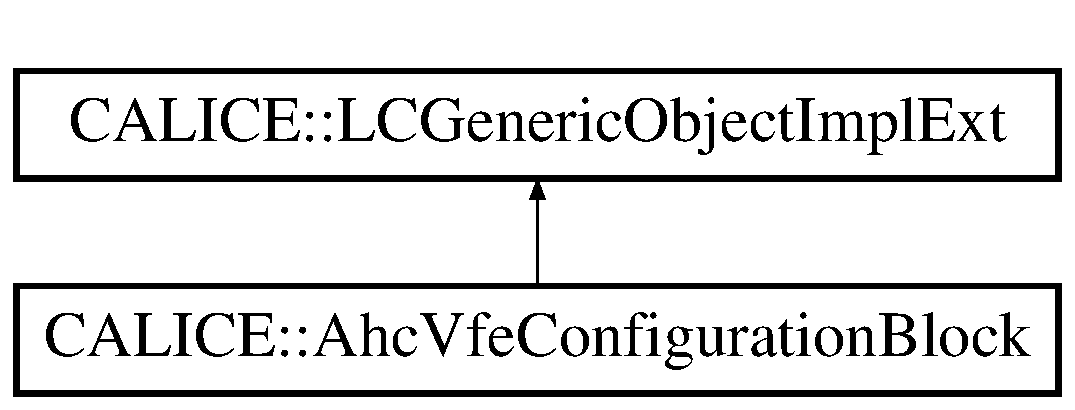
\includegraphics[height=2cm]{classCALICE_1_1AhcVfeConfigurationBlock}
\end{center}
\end{figure}
\subsection*{Public Member Functions}
\begin{DoxyCompactItemize}
\item 
{\bf AhcVfeConfigurationBlock} (int boardID)
\begin{DoxyCompactList}\small\item\em Convenient c'tor. \item\end{DoxyCompactList}\item 
{\bf AhcVfeConfigurationBlock} \& {\bf setCrateID} (short crateID)\label{classCALICE_1_1AhcVfeConfigurationBlock_a201e36bf403cffb9903f1566be72818e}

\begin{DoxyCompactList}\small\item\em Set the crateID. \item\end{DoxyCompactList}\item 
short {\bf getCrateID} () const \label{classCALICE_1_1AhcVfeConfigurationBlock_a19695e1a48f9901745283f645c813a59}

\begin{DoxyCompactList}\small\item\em Get the crate ID. \item\end{DoxyCompactList}\item 
{\bf AhcVfeConfigurationBlock} \& {\bf setSlotID} (short slotID)\label{classCALICE_1_1AhcVfeConfigurationBlock_a6ef47b059a3b1d255c99df87c30782d2}

\begin{DoxyCompactList}\small\item\em Set the Slot ID. \item\end{DoxyCompactList}\item 
short {\bf getSlotID} () const \label{classCALICE_1_1AhcVfeConfigurationBlock_adba054e559e65594f1477cd578a4230e}

\begin{DoxyCompactList}\small\item\em Get the Slot ID. \item\end{DoxyCompactList}\item 
{\bf AhcVfeConfigurationBlock} \& {\bf setBoardComponentNumber} (short componentNumber)\label{classCALICE_1_1AhcVfeConfigurationBlock_a30f5dff217b1fa44326c86902c1b88ee}

\begin{DoxyCompactList}\small\item\em Set the BoardComponentNumber. \item\end{DoxyCompactList}\item 
short {\bf getBoardComponentNumber} () const \label{classCALICE_1_1AhcVfeConfigurationBlock_a434b41151c72986819bf924ae024345c}

\begin{DoxyCompactList}\small\item\em Get the BoardComponentNumber. \item\end{DoxyCompactList}\item 
void {\bf setRecordLabel} (int label)\label{classCALICE_1_1AhcVfeConfigurationBlock_ab74486109cf73a0bae48ef7a222a73cb}

\begin{DoxyCompactList}\small\item\em Set the Record Label. \item\end{DoxyCompactList}\item 
short {\bf getRecordLabel} () const \label{classCALICE_1_1AhcVfeConfigurationBlock_a95166f80fa388544cefd9bff2bcdf83c}

\begin{DoxyCompactList}\small\item\em Get the Record Label. \item\end{DoxyCompactList}\item 
{\bf AhcVfeConfigurationBlock} \& {\bf setBoardID} (int boardID)\label{classCALICE_1_1AhcVfeConfigurationBlock_a4ac33c3ed60f3fb3fd20e3ba993ee515}

\begin{DoxyCompactList}\small\item\em Set the board ID. \item\end{DoxyCompactList}\item 
int {\bfseries getBoardID} () const \label{classCALICE_1_1AhcVfeConfigurationBlock_ac2842de93b26e2b33512debed50b48b2}

\item 
{\bf AhcVfeConfigurationBlock} (LCObject $\ast$obj)\label{classCALICE_1_1AhcVfeConfigurationBlock_a368a7db6a5636970f2966b9b544efcb0}

\begin{DoxyCompactList}\small\item\em 'Copy constructor' needed to interpret LCCollection read from file/database. \item\end{DoxyCompactList}\item 
{\bf AhcVfeConfigurationBlock} \& {\bf setVerificationData} (int verifData)\label{classCALICE_1_1AhcVfeConfigurationBlock_a0c2a00f1d35ab1a2049fd5c056f30b26}

\begin{DoxyCompactList}\small\item\em Set Vfe Verification Data. \item\end{DoxyCompactList}\item 
unsigned int {\bf getVerificationData} ()\label{classCALICE_1_1AhcVfeConfigurationBlock_ada572f7f63fb95508b50a2893f6dd418}

\begin{DoxyCompactList}\small\item\em Get Vfe Verification Data. \item\end{DoxyCompactList}\item 
{\bf AhcVfeConfigurationBlock} \& {\bf setShiftRegisterData} (int ipos, int ival)\label{classCALICE_1_1AhcVfeConfigurationBlock_abd1529f8eaaa39f8a9e9c3b6d70c614d}

\begin{DoxyCompactList}\small\item\em Set the Shiftregister data. \item\end{DoxyCompactList}\item 
bool {\bfseries isCoarseLayer} ()\label{classCALICE_1_1AhcVfeConfigurationBlock_ac95e9cd52673830425cb41130f9fb9fd}

\item 
int {\bf getShiftRegisterData} (int ipos)\label{classCALICE_1_1AhcVfeConfigurationBlock_a0ee9e9c4be33ee5146a4d979e1949026}

\begin{DoxyCompactList}\small\item\em Get the Shiftregister data. \item\end{DoxyCompactList}\item 
void {\bf print} (std::ostream \&os)\label{classCALICE_1_1AhcVfeConfigurationBlock_a1762058d56a4bed8fe64599bd7473f3c}

\begin{DoxyCompactList}\small\item\em Convenient print method. \item\end{DoxyCompactList}\item 
const std::string {\bf getTypeName} () const \label{classCALICE_1_1AhcVfeConfigurationBlock_a9644528d361e0a8a548a2feb34f02f92}

\begin{DoxyCompactList}\small\item\em Return the type of the class. \item\end{DoxyCompactList}\item 
const std::string {\bf getDataDescription} () const \label{classCALICE_1_1AhcVfeConfigurationBlock_a3fa9acfa0903309b37d23d22c30cf165}

\begin{DoxyCompactList}\small\item\em Return a brief description of the data members. \item\end{DoxyCompactList}\end{DoxyCompactItemize}
\subsection*{Static Public Member Functions}
\begin{DoxyCompactItemize}
\item 
static unsigned int {\bfseries makeBoardID} (const short crateID, const short slotID, const short boardComponentNumber)\label{classCALICE_1_1AhcVfeConfigurationBlock_a7073a54fe28524a7accbe91606eee989}

\end{DoxyCompactItemize}


\subsection{Detailed Description}
Interface Class to access the AhcVfeConfigurationData. \begin{DoxyAuthor}{Author}
Roman P�schl DESY 
\end{DoxyAuthor}
\begin{DoxyDate}{Date}
Nov 2005 
\end{DoxyDate}


Definition at line 33 of file AhcVfeConfigurationBlock.hh.

\subsection{Constructor \& Destructor Documentation}
\index{CALICE::AhcVfeConfigurationBlock@{CALICE::AhcVfeConfigurationBlock}!AhcVfeConfigurationBlock@{AhcVfeConfigurationBlock}}
\index{AhcVfeConfigurationBlock@{AhcVfeConfigurationBlock}!CALICE::AhcVfeConfigurationBlock@{CALICE::AhcVfeConfigurationBlock}}
\subsubsection[{AhcVfeConfigurationBlock}]{\setlength{\rightskip}{0pt plus 5cm}CALICE::AhcVfeConfigurationBlock::AhcVfeConfigurationBlock (int {\em boardID})\hspace{0.3cm}{\ttfamily  [inline]}}\label{classCALICE_1_1AhcVfeConfigurationBlock_ae545b6dfccdb15c9af4ac0243e9898f4}


Convenient c'tor. 
\begin{DoxyParams}{Parameters}
\item[{\em boardID}]CERC board ID (VME crate channel)) \end{DoxyParams}


Definition at line 46 of file AhcVfeConfigurationBlock.hh.

References CALICE::LCGenericObjectImplExt::obj().

The documentation for this class was generated from the following file:\begin{DoxyCompactItemize}
\item 
AhcVfeConfigurationBlock.hh\end{DoxyCompactItemize}

\section{CALICE::Alignment Class Reference}
\label{classCALICE_1_1Alignment}\index{CALICE::Alignment@{CALICE::Alignment}}


Class to comunicate/handle the translation into unique layer/cell ids and 3D spacial coordinates.  


{\ttfamily \#include $<$Alignment.hh$>$}Inheritance diagram for CALICE::Alignment::\begin{figure}[H]
\begin{center}
\leavevmode
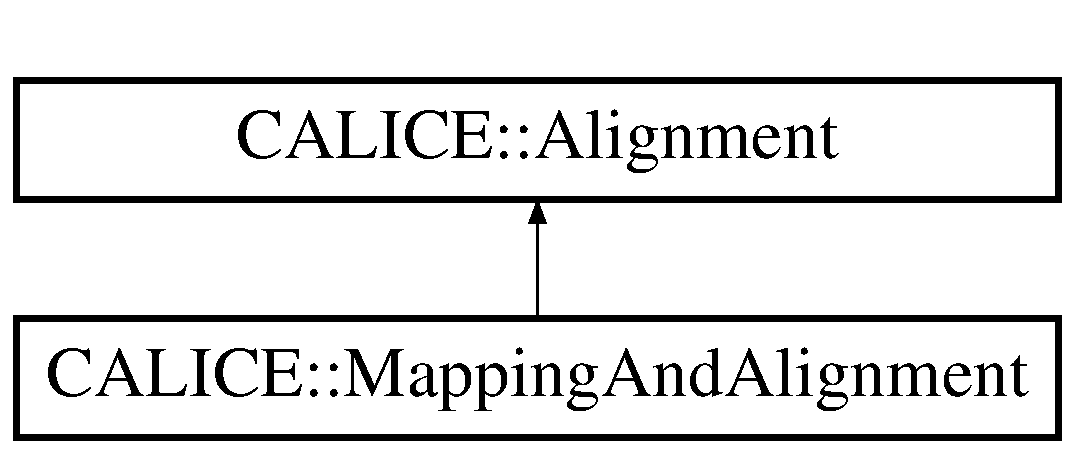
\includegraphics[height=2cm]{classCALICE_1_1Alignment}
\end{center}
\end{figure}
\subsection*{Public Member Functions}
\begin{DoxyCompactItemize}
\item 
{\bf Alignment} ()
\begin{DoxyCompactList}\small\item\em default constructor. \item\end{DoxyCompactList}\item 
void {\bf init} ()\label{classCALICE_1_1Alignment_adad093be57011962ceaa0dc6fd597759}

\begin{DoxyCompactList}\small\item\em Does nothing for the time being. \item\end{DoxyCompactList}\item 
UInt\_\-t {\bf getGeometricalCellIndex} (UInt\_\-t module\_\-index, UInt\_\-t cell\_\-index) const 
\begin{DoxyCompactList}\small\item\em Get the unique cell index of the cell specified by the module and the cell index. \item\end{DoxyCompactList}\item 
bool {\bf isValid} (UInt\_\-t module\_\-index) const 
\begin{DoxyCompactList}\small\item\em Return true if the type of the given module is valid. \item\end{DoxyCompactList}\item 
UChar\_\-t {\bf getModuleType} (UInt\_\-t module\_\-index) const 
\begin{DoxyCompactList}\small\item\em Get the type of a certain module. \item\end{DoxyCompactList}\item 
{\bf ThreeVector\_\-t} {\bfseries getPosition} (UInt\_\-t module\_\-index, UInt\_\-t cell\_\-index) const \label{classCALICE_1_1Alignment_a3ddad6c8a5aeaed18d3529d212d3ba1b}

\item 
{\bf ThreeVector\_\-t} {\bfseries transformPosition} ({\bf ThreeVector\_\-t} \&a\_\-position) const \label{classCALICE_1_1Alignment_a77b2bfc80a819a597a8e451a2bbf7655}

\item 
UInt\_\-t {\bfseries getNModules} () const \label{classCALICE_1_1Alignment_a439df763fea328d7f58336f3b97ca786}

\item 
Bool\_\-t {\bf isModule} (UInt\_\-t module\_\-index) const \label{classCALICE_1_1Alignment_a4860425f1c86fbc897920647f0dd7451}

\begin{DoxyCompactList}\small\item\em Return false if the module index is out of range. \item\end{DoxyCompactList}\item 
const {\bf ModuleDescription} \& {\bf getModuleDescription} (UInt\_\-t module\_\-index) const 
\begin{DoxyCompactList}\small\item\em Return the description object for the given module. \item\end{DoxyCompactList}\item 
UInt\_\-t {\bfseries getNCellsPerModule} (UInt\_\-t module\_\-index) const \label{classCALICE_1_1Alignment_a67d96a33524e3dd7e4c151943caa103c}

\item 
Float\_\-t {\bf getModuleWidth} (UInt\_\-t module\_\-index) const \label{classCALICE_1_1Alignment_a2a3b34cd5399e9d4c6c34737314a42e7}

\begin{DoxyCompactList}\small\item\em Get the cell width of the given module and cell. \item\end{DoxyCompactList}\item 
Float\_\-t {\bf getModuleHeight} (UInt\_\-t module\_\-index) const \label{classCALICE_1_1Alignment_a5112553b1a361f609e186c85f97d0f7f}

\begin{DoxyCompactList}\small\item\em Get the cell width of the given module and cell. \item\end{DoxyCompactList}\item 
Float\_\-t {\bf getCellWidth} (UInt\_\-t module\_\-index, UInt\_\-t cell\_\-index) const \label{classCALICE_1_1Alignment_a7ed4ffe8bed99bed35d69c0ac431bc67}

\begin{DoxyCompactList}\small\item\em Get the cell width of the given module and cell. \item\end{DoxyCompactList}\item 
Float\_\-t {\bf getCellHeight} (UInt\_\-t module\_\-index, UInt\_\-t cell\_\-index) const 
\begin{DoxyCompactList}\small\item\em Get the cell width of the given module. \item\end{DoxyCompactList}\item 
{\bf ThreeVector\_\-t} {\bf getPosition} () const \label{classCALICE_1_1Alignment_a8264e5dd81a84e2362f8cc4d26a4c41f}

\begin{DoxyCompactList}\small\item\em Get the position of the detector in its proper coordinate system. \item\end{DoxyCompactList}\item 
{\bf ThreeVector\_\-t} {\bf getModuleProperCenter} (UInt\_\-t module\_\-index) const \label{classCALICE_1_1Alignment_a696dfaa32cdaf473b07c981934598958}

\begin{DoxyCompactList}\small\item\em Get the upper right corner of a module. \item\end{DoxyCompactList}\item 
{\bf ThreeVector\_\-t} {\bf getModuleProperPosition} (UInt\_\-t module\_\-index) const \label{classCALICE_1_1Alignment_ab46ad7e1e3e78dc47fcc4549a231c23e}

\begin{DoxyCompactList}\small\item\em Get the position of a module in the proper coordinate system of the detector. \item\end{DoxyCompactList}\item 
{\bf ThreeVector\_\-t} {\bf getModulePosition} (UInt\_\-t module\_\-index) const \label{classCALICE_1_1Alignment_a1ecf26def8a818e1f6035c9e18653d28}

\begin{DoxyCompactList}\small\item\em Get the position of a module in the reference coordinate system. \item\end{DoxyCompactList}\item 
{\bf ThreeVector\_\-t} {\bf getModuleCenter} (UInt\_\-t module\_\-index) const \label{classCALICE_1_1Alignment_a4dd6c5cde6371a0b26c6438adf54414f}

\begin{DoxyCompactList}\small\item\em Get the center of a module in the reference coordinate system. \item\end{DoxyCompactList}\item 
Float\_\-t {\bf getDetectorAngleZX} () const \label{classCALICE_1_1Alignment_a10d5e1ddf0c26a74421c22774248671d}

\begin{DoxyCompactList}\small\item\em Return the effective rotation angle of the detector. \item\end{DoxyCompactList}\item 
virtual void {\bf moduleTypeChanged} (lcio::LCCollection $\ast$col)
\begin{DoxyCompactList}\small\item\em Inform the object about changes of the module types. \item\end{DoxyCompactList}\item 
virtual void {\bf moduleLocationChanged} (lcio::LCCollection $\ast$col)
\begin{DoxyCompactList}\small\item\em Inform the object about changes of the module locations. \item\end{DoxyCompactList}\item 
virtual void {\bf stagePositionChanged} (lcio::LCCollection $\ast$col)
\begin{DoxyCompactList}\small\item\em Inform the object about changes in the stage positions on which the detector is mounted. \item\end{DoxyCompactList}\item 
virtual void {\bf detectorTransformation} (lcio::LCCollection $\ast$col)
\begin{DoxyCompactList}\small\item\em Inform the object about changes of the detector position and rotation. \item\end{DoxyCompactList}\item 
virtual void {\bf referenceTransformation} (lcio::LCCollection $\ast$col)
\begin{DoxyCompactList}\small\item\em Inform the object about changes of the reference position and rotation. \item\end{DoxyCompactList}\item 
UInt\_\-t {\bf getCellIndexOffset} (UInt\_\-t module\_\-index) const \label{classCALICE_1_1Alignment_ad07573bf525c2271792bc040242632a2}

\begin{DoxyCompactList}\small\item\em Get the cell index offset of a module. \item\end{DoxyCompactList}\end{DoxyCompactItemize}
\subsection*{Protected Types}
\begin{DoxyCompactItemize}
\item 
typedef {\bf SimpleArray\_\-t}$<$ pair$<$ UInt\_\-t, {\bf ModuleLocation} $>$ $>$ {\bf ModuleList\_\-t}
\begin{DoxyCompactList}\small\item\em Defined module locations (not necessarily connected to a front-\/end. \item\end{DoxyCompactList}\item 
typedef {\bf SimpleArray\_\-t}$<$ {\bf ModuleDescription} $>$ {\bfseries ModuleTypeList\_\-t}\label{classCALICE_1_1Alignment_a10d63d19612d0b5384bfc7f9b7f84bbd}

\end{DoxyCompactItemize}
\subsection*{Protected Attributes}
\begin{DoxyCompactItemize}
\item 
{\bf ModuleList\_\-t} {\bfseries \_\-moduleLocationList}\label{classCALICE_1_1Alignment_a7038cce4a5b2baf25597867f0b5407c5}

\item 
{\bf ModuleTypeList\_\-t} {\bfseries \_\-moduleTypeList}\label{classCALICE_1_1Alignment_a975a8333c0f374f44dee0fa6c37cf732}

\end{DoxyCompactItemize}
\subsection*{Private Types}
\begin{DoxyCompactItemize}
\item 
enum {\bfseries ETransformation} \{ {\bfseries kDetector}, 
{\bfseries kReference}, 
{\bfseries kEffective}, 
{\bfseries kNTransformations}
 \}
\item 
typedef void(Alignment::$\ast$ {\bf StageChangeHandleFunc\_\-t} )(lcio::LCCollection $\ast$col)\label{classCALICE_1_1Alignment_a5131ddec8fd42fefa45de5826aecd4c1}

\begin{DoxyCompactList}\small\item\em A map which holds pointers to functions to access the parameters of teh movable stage(s). \item\end{DoxyCompactList}\end{DoxyCompactItemize}
\subsection*{Private Member Functions}
\begin{DoxyCompactItemize}
\item 
void {\bf setTransformation} (lcio::LCCollection $\ast$col, ETransformation transformation\_\-type)\label{classCALICE_1_1Alignment_adb7fd43e529d374f41e8be0a1610faf9}

\begin{DoxyCompactList}\small\item\em Set the transformation parameters from the conditions data collection. \item\end{DoxyCompactList}\item 
void {\bf calculateEffectiveTransformation} ()
\begin{DoxyCompactList}\small\item\em Calculate the effective transformation from the detector and reference transformation. \item\end{DoxyCompactList}\item 
void {\bfseries handleEmcStage} (LCCollection $\ast$)\label{classCALICE_1_1Alignment_abf5097c7e86a04e285cd59ddf8848c47}

\item 
void {\bfseries handleAhcStage} (LCCollection $\ast$)\label{classCALICE_1_1Alignment_a907fd80bfc25e5f98b6ebab3fb7533fa}

\end{DoxyCompactItemize}
\subsection*{Private Attributes}
\begin{DoxyCompactItemize}
\item 
Float\_\-t {\bf \_\-detectorPos} [kNTransformations][3]\label{classCALICE_1_1Alignment_a6f73f5a4df2e1b7fd2a3da7c99d70d51}

\begin{DoxyCompactList}\small\item\em the position of the detector \item\end{DoxyCompactList}\item 
Float\_\-t {\bf \_\-detectorAngleZX} [kNTransformations]
\begin{DoxyCompactList}\small\item\em configuration angle w.r.t. \item\end{DoxyCompactList}\item 
Double\_\-t {\bf \_\-detectorAngleZXSin}\label{classCALICE_1_1Alignment_a398120953f6f68d96563c57dd95e12aa}

\begin{DoxyCompactList}\small\item\em sin of the effective rotation angle in the z-\/x plane \item\end{DoxyCompactList}\item 
Double\_\-t {\bf \_\-detectorAngleZXCos}\label{classCALICE_1_1Alignment_a4b7a1cc57b53c53a0f251dae7782f675}

\begin{DoxyCompactList}\small\item\em cos of the effective rotation angle in the z-\/x plane \item\end{DoxyCompactList}\item 
Float\_\-t {\bf \_\-detectorRotationX0} [kNTransformations]\label{classCALICE_1_1Alignment_a5b7bee79b2ad35a2e7b128f841a1fd64}

\begin{DoxyCompactList}\small\item\em origin of the detector ratation (x-\/direction) \item\end{DoxyCompactList}\item 
Float\_\-t {\bf \_\-detectorRotationZ0} [kNTransformations]\label{classCALICE_1_1Alignment_a2faba0894844b8779abd31d7e8a56854}

\begin{DoxyCompactList}\small\item\em origin of the detector ratation (z-\/direction) \item\end{DoxyCompactList}\item 
std::map$<$ std::string, {\bf StageChangeHandleFunc\_\-t} $>$ {\bfseries \_\-knownStageTypes}\label{classCALICE_1_1Alignment_a3b409667846fdd3b1b36abca4e74ba8d}

\item 
float {\bf \_\-stageOffset\_\-x}\label{classCALICE_1_1Alignment_a38bc228c141775137178ab1c171a4c92}

\begin{DoxyCompactList}\small\item\em The offsets due to the movable stage. \item\end{DoxyCompactList}\item 
float {\bfseries \_\-stageOffset\_\-y}\label{classCALICE_1_1Alignment_a734151cd0b80de77cd16cce5b7ae9106}

\end{DoxyCompactItemize}
\subsection*{Static Private Attributes}
\begin{DoxyCompactItemize}
\item 
static const Double\_\-t {\bfseries \_\-\_\-degToRad} = M\_\-PI/180.\label{classCALICE_1_1Alignment_af48cedd060a33b725e5f14f81f3033d1}

\end{DoxyCompactItemize}


\subsection{Detailed Description}
Class to comunicate/handle the translation into unique layer/cell ids and 3D spacial coordinates. The class has to be informed about changes of the detector configuration using the methods \doxyref{CALICE::Alignment::moduleTypeChanged}{p.}{classCALICE_1_1Alignment_adc041696a184db384a57bca51df7bc25}, \doxyref{CALICE::Alignment::moduleLocationChanged}{p.}{classCALICE_1_1Alignment_a3ea188d0a90c7e0881d735cf55ef5604}, \doxyref{CALICE::MappingAndAlignment::moduleConnectionChanged}{p.}{classCALICE_1_1MappingAndAlignment_a3717c2ea27a5a60ff2a41d17803ff148} and Alignment::experimentalSetup. This information is used to map the DAQ signals to cells and calculate 3D spacial coordinates for hits.

The class performs range checks only if BOUNDARY\_\-CHECK is defined. 

Definition at line 42 of file Alignment.hh.

\subsection{Member Typedef Documentation}
\index{CALICE::Alignment@{CALICE::Alignment}!ModuleList\_\-t@{ModuleList\_\-t}}
\index{ModuleList\_\-t@{ModuleList\_\-t}!CALICE::Alignment@{CALICE::Alignment}}
\subsubsection[{ModuleList\_\-t}]{\setlength{\rightskip}{0pt plus 5cm}typedef {\bf SimpleArray\_\-t}$<$pair$<$UInt\_\-t,{\bf ModuleLocation}$>$ $>$ {\bf CALICE::Alignment::ModuleList\_\-t}\hspace{0.3cm}{\ttfamily  [protected]}}\label{classCALICE_1_1Alignment_ad0153c70861a5bc9976bc21983ac319f}


Defined module locations (not necessarily connected to a front-\/end. First component contains the module ID, the second the module location information. 

Definition at line 475 of file Alignment.hh.

\subsection{Constructor \& Destructor Documentation}
\index{CALICE::Alignment@{CALICE::Alignment}!Alignment@{Alignment}}
\index{Alignment@{Alignment}!CALICE::Alignment@{CALICE::Alignment}}
\subsubsection[{Alignment}]{\setlength{\rightskip}{0pt plus 5cm}CALICE::Alignment::Alignment ()}\label{classCALICE_1_1Alignment_a9301ea57c3cf0bf16154f67e45023385}


default constructor. The default constructor configures the conditions data change delegators. 

Definition at line 29 of file Alignment.cc.

References setTransformation().

\subsection{Member Function Documentation}
\index{CALICE::Alignment@{CALICE::Alignment}!calculateEffectiveTransformation@{calculateEffectiveTransformation}}
\index{calculateEffectiveTransformation@{calculateEffectiveTransformation}!CALICE::Alignment@{CALICE::Alignment}}
\subsubsection[{calculateEffectiveTransformation}]{\setlength{\rightskip}{0pt plus 5cm}void CALICE::Alignment::calculateEffectiveTransformation ()\hspace{0.3cm}{\ttfamily  [private]}}\label{classCALICE_1_1Alignment_af778a021450c0087cbf459eb291aa8f1}


Calculate the effective transformation from the detector and reference transformation. 

Definition at line 171 of file Alignment.cc.

References \_\-detectorAngleZX, \_\-detectorAngleZXCos, \_\-detectorAngleZXSin, \_\-detectorPos, \_\-detectorRotationX0, and \_\-detectorRotationZ0.

Referenced by setTransformation().\index{CALICE::Alignment@{CALICE::Alignment}!detectorTransformation@{detectorTransformation}}
\index{detectorTransformation@{detectorTransformation}!CALICE::Alignment@{CALICE::Alignment}}
\subsubsection[{detectorTransformation}]{\setlength{\rightskip}{0pt plus 5cm}virtual void CALICE::Alignment::detectorTransformation (lcio::LCCollection $\ast$ {\em col})\hspace{0.3cm}{\ttfamily  [inline, virtual]}}\label{classCALICE_1_1Alignment_a85a9ad1e7e95e2ade18f30e6373eadfa}


Inform the object about changes of the detector position and rotation. 
\begin{DoxyParams}{Parameters}
\item[{\em col}]collection of \doxyref{DetectorTransformation}{p.}{classCALICE_1_1DetectorTransformation} objects This class must be called before querying the postion of cells. The position is calculated in the reference coorindate system. \end{DoxyParams}


Definition at line 457 of file Alignment.hh.

References setTransformation().\index{CALICE::Alignment@{CALICE::Alignment}!getCellHeight@{getCellHeight}}
\index{getCellHeight@{getCellHeight}!CALICE::Alignment@{CALICE::Alignment}}
\subsubsection[{getCellHeight}]{\setlength{\rightskip}{0pt plus 5cm}Float\_\-t CALICE::Alignment::getCellHeight (UInt\_\-t {\em module\_\-index}, \/  UInt\_\-t {\em cell\_\-index}) const\hspace{0.3cm}{\ttfamily  [inline]}}\label{classCALICE_1_1Alignment_a84ad3b3ffba7850de98971a51eeba82f}


Get the cell width of the given module. It is assumed that the cells of one module all have the same width. 

Definition at line 325 of file Alignment.hh.\index{CALICE::Alignment@{CALICE::Alignment}!getGeometricalCellIndex@{getGeometricalCellIndex}}
\index{getGeometricalCellIndex@{getGeometricalCellIndex}!CALICE::Alignment@{CALICE::Alignment}}
\subsubsection[{getGeometricalCellIndex}]{\setlength{\rightskip}{0pt plus 5cm}UInt\_\-t CALICE::Alignment::getGeometricalCellIndex (UInt\_\-t {\em module\_\-index}, \/  UInt\_\-t {\em cell\_\-index}) const\hspace{0.3cm}{\ttfamily  [inline]}}\label{classCALICE_1_1Alignment_add6b290637455010456ce6f643ccb34f}


Get the unique cell index of the cell specified by the module and the cell index. 
\begin{DoxyParams}{Parameters}
\item[{\em module\_\-index}]unique index for modules which should run from 0..total number of modules \item[{\em cell\_\-index}]within the module (0.. number of cells of this module type) \end{DoxyParams}
\begin{DoxyReturn}{Returns}
unique cell index. 
\end{DoxyReturn}

\begin{DoxyExceptions}{Exceptions}
\item[{\em range\_\-error}]if the module index is out of range and BOUNDARY\_\-CHECK is defined\end{DoxyExceptions}
The cell index conforms to the Mokka specification (see for example \doxyref{CellIndex}{p.}{classCALICE_1_1CellIndex}). It is composed of the layer number, the wafer column and row, and the pad column and row. 

Definition at line 68 of file Alignment.hh.\index{CALICE::Alignment@{CALICE::Alignment}!getModuleDescription@{getModuleDescription}}
\index{getModuleDescription@{getModuleDescription}!CALICE::Alignment@{CALICE::Alignment}}
\subsubsection[{getModuleDescription}]{\setlength{\rightskip}{0pt plus 5cm}const {\bf ModuleDescription}\& CALICE::Alignment::getModuleDescription (UInt\_\-t {\em module\_\-index}) const\hspace{0.3cm}{\ttfamily  [inline]}}\label{classCALICE_1_1Alignment_a6ac1899ddab2b35464b85ec39a67ede7}


Return the description object for the given module. 
\begin{DoxyParams}{Parameters}
\item[{\em module\_\-index}]the index of the moduel. \end{DoxyParams}


Definition at line 229 of file Alignment.hh.\index{CALICE::Alignment@{CALICE::Alignment}!getModuleType@{getModuleType}}
\index{getModuleType@{getModuleType}!CALICE::Alignment@{CALICE::Alignment}}
\subsubsection[{getModuleType}]{\setlength{\rightskip}{0pt plus 5cm}UChar\_\-t CALICE::Alignment::getModuleType (UInt\_\-t {\em module\_\-index}) const\hspace{0.3cm}{\ttfamily  [inline]}}\label{classCALICE_1_1Alignment_a6347626acbfc5dfcbca3c97c89fcad70}


Get the type of a certain module. The module type together with the module ID uniquly identifies a module. Different modules of one type always have different IDs but modules of different types may have the same ID. In case of the ECAL the module ID is the serial number of the PCBs. 
\begin{DoxyParams}{Parameters}
\item[{\em module\_\-index}]the index of the module within the detector (not necessarily the same as the module ID) \end{DoxyParams}
\begin{DoxyReturn}{Returns}
the module type 
\end{DoxyReturn}

\begin{DoxyExceptions}{Exceptions}
\item[{\em range\_\-error}]if the module specified by module\_\-index is not defined but only if BOUNDARY\_\-CHECK is defined. \end{DoxyExceptions}
\begin{DoxySeeAlso}{See also}
getModuleID() 
\end{DoxySeeAlso}


Definition at line 114 of file Alignment.hh.

Referenced by CALICE::MappingAndAlignment::print().\index{CALICE::Alignment@{CALICE::Alignment}!isValid@{isValid}}
\index{isValid@{isValid}!CALICE::Alignment@{CALICE::Alignment}}
\subsubsection[{isValid}]{\setlength{\rightskip}{0pt plus 5cm}bool CALICE::Alignment::isValid (UInt\_\-t {\em module\_\-index}) const\hspace{0.3cm}{\ttfamily  [inline]}}\label{classCALICE_1_1Alignment_a3b3a82a744ce67860086203baef3ddff}


Return true if the type of the given module is valid. 
\begin{DoxyParams}{Parameters}
\item[{\em module\_\-index}]the index of the given module. \end{DoxyParams}


Definition at line 90 of file Alignment.hh.

Referenced by CALICE::MappingAndAlignment::print().\index{CALICE::Alignment@{CALICE::Alignment}!moduleLocationChanged@{moduleLocationChanged}}
\index{moduleLocationChanged@{moduleLocationChanged}!CALICE::Alignment@{CALICE::Alignment}}
\subsubsection[{moduleLocationChanged}]{\setlength{\rightskip}{0pt plus 5cm}void CALICE::Alignment::moduleLocationChanged (lcio::LCCollection $\ast$ {\em col})\hspace{0.3cm}{\ttfamily  [virtual]}}\label{classCALICE_1_1Alignment_a3ea188d0a90c7e0881d735cf55ef5604}


Inform the object about changes of the module locations. 
\begin{DoxyParams}{Parameters}
\item[{\em col}]collection of \doxyref{ModuleLocation}{p.}{classCALICE_1_1ModuleLocation} objects This class must be called before using any(most) of the other methods. The function call will cause a rebuild of the module DAQ front-\/end connection tree. \end{DoxyParams}


Reimplemented in {\bf CALICE::MappingAndAlignment} \doxyref{}{p.}{classCALICE_1_1MappingAndAlignment_ab9d17873aeb090388556547cb6b67ba8}.

Definition at line 76 of file Alignment.cc.\index{CALICE::Alignment@{CALICE::Alignment}!moduleTypeChanged@{moduleTypeChanged}}
\index{moduleTypeChanged@{moduleTypeChanged}!CALICE::Alignment@{CALICE::Alignment}}
\subsubsection[{moduleTypeChanged}]{\setlength{\rightskip}{0pt plus 5cm}void CALICE::Alignment::moduleTypeChanged (lcio::LCCollection $\ast$ {\em col})\hspace{0.3cm}{\ttfamily  [virtual]}}\label{classCALICE_1_1Alignment_adc041696a184db384a57bca51df7bc25}


Inform the object about changes of the module types. 
\begin{DoxyParams}{Parameters}
\item[{\em col}]collection of \doxyref{ModuleDescription}{p.}{classCALICE_1_1ModuleDescription} objects This class must be called before using any(most) of the other methods. The function call will cause a rebuild of the module DAQ front-\/end connection tree. \end{DoxyParams}


Reimplemented in {\bf CALICE::MappingAndAlignment} \doxyref{}{p.}{classCALICE_1_1MappingAndAlignment_a5564c399de481a023b702a39a04fea7f}.

Definition at line 47 of file Alignment.cc.\index{CALICE::Alignment@{CALICE::Alignment}!referenceTransformation@{referenceTransformation}}
\index{referenceTransformation@{referenceTransformation}!CALICE::Alignment@{CALICE::Alignment}}
\subsubsection[{referenceTransformation}]{\setlength{\rightskip}{0pt plus 5cm}virtual void CALICE::Alignment::referenceTransformation (lcio::LCCollection $\ast$ {\em col})\hspace{0.3cm}{\ttfamily  [inline, virtual]}}\label{classCALICE_1_1Alignment_aedf5694bbb286510411e1de986e51ac5}


Inform the object about changes of the reference position and rotation. 
\begin{DoxyParams}{Parameters}
\item[{\em col}]collection of \doxyref{DetectorTransformation}{p.}{classCALICE_1_1DetectorTransformation} objects This class must be called before querying the postion of cells. The position is calculated in the reference coordinate system. \end{DoxyParams}


Definition at line 466 of file Alignment.hh.

References setTransformation().\index{CALICE::Alignment@{CALICE::Alignment}!stagePositionChanged@{stagePositionChanged}}
\index{stagePositionChanged@{stagePositionChanged}!CALICE::Alignment@{CALICE::Alignment}}
\subsubsection[{stagePositionChanged}]{\setlength{\rightskip}{0pt plus 5cm}void CALICE::Alignment::stagePositionChanged (lcio::LCCollection $\ast$ {\em col})\hspace{0.3cm}{\ttfamily  [virtual]}}\label{classCALICE_1_1Alignment_ab018d115126785360ec8e70fb710409b}


Inform the object about changes in the stage positions on which the detector is mounted. 
\begin{DoxyParams}{Parameters}
\item[{\em col}]collection of StageParameters objects This class must be called before calculating the actual cell positions The function will provide the xy values for a correct transversal alignment of the detectors. \end{DoxyParams}


Definition at line 218 of file Alignment.cc.

\subsection{Field Documentation}
\index{CALICE::Alignment@{CALICE::Alignment}!\_\-detectorAngleZX@{\_\-detectorAngleZX}}
\index{\_\-detectorAngleZX@{\_\-detectorAngleZX}!CALICE::Alignment@{CALICE::Alignment}}
\subsubsection[{\_\-detectorAngleZX}]{\setlength{\rightskip}{0pt plus 5cm}Float\_\-t {\bf CALICE::Alignment::\_\-detectorAngleZX}[kNTransformations]\hspace{0.3cm}{\ttfamily  [private]}}\label{classCALICE_1_1Alignment_a7580f22b535e4538967b0ef80f22f3ed}


configuration angle w.r.t. to the beam axis in the horizontal plane 

Definition at line 501 of file Alignment.hh.

Referenced by calculateEffectiveTransformation(), getDetectorAngleZX(), and setTransformation().

The documentation for this class was generated from the following files:\begin{DoxyCompactItemize}
\item 
Alignment.hh\item 
Alignment.cc\end{DoxyCompactItemize}

\section{Average\_\-t Class Reference}
\label{classAverage__t}\index{Average\_\-t@{Average\_\-t}}


Calculate mean and standard deviation and find minimum and maximum value.  


{\ttfamily \#include $<$Average\_\-t.hh$>$}\subsection*{Public Member Functions}
\begin{DoxyCompactItemize}
\item 
{\bf Average\_\-t} ()\label{classAverage__t_aa221818a7a022083297e9cab811252e6}

\begin{DoxyCompactList}\small\item\em Default constructor initialses all arrays to be ready to gather statastics of a variable. \item\end{DoxyCompactList}\item 
void {\bf add} (Float\_\-t value, Float\_\-t weight=1.)
\begin{DoxyCompactList}\small\item\em Build the sum and the sum of squares and find the minimum and maximum value. \item\end{DoxyCompactList}\item 
void {\bf calculate} ()
\begin{DoxyCompactList}\small\item\em Calculate the standard deviation and the mean. \item\end{DoxyCompactList}\item 
Double\_\-t {\bf mean} () const 
\begin{DoxyCompactList}\small\item\em Return the mean value. \item\end{DoxyCompactList}\item 
Double\_\-t {\bf sigma} () const 
\begin{DoxyCompactList}\small\item\em Return the standard deviation. \item\end{DoxyCompactList}\item 
Float\_\-t {\bf min} () const \label{classAverage__t_a7ca3e52df15cd84cd40b8456f3d505e8}

\begin{DoxyCompactList}\small\item\em Return the minimum value. \item\end{DoxyCompactList}\item 
Float\_\-t {\bf max} () const \label{classAverage__t_a1cfde99d82e467a5f6adf92d51955225}

\begin{DoxyCompactList}\small\item\em Return the maximum value. \item\end{DoxyCompactList}\item 
Double\_\-t {\bf weight} () const \label{classAverage__t_a3c8ebca4ecd924335737f7aacef198f7}

\begin{DoxyCompactList}\small\item\em Get the total accumulated weight. \item\end{DoxyCompactList}\item 
Double\_\-t {\bf sum} () const \label{classAverage__t_aeb4e2a1c2ddac4ed9cc055689c911a49}

\begin{DoxyCompactList}\small\item\em Get the total accumulated data. \item\end{DoxyCompactList}\end{DoxyCompactItemize}
\subsection*{Protected Attributes}
\begin{DoxyCompactItemize}
\item 
Double\_\-t {\bfseries \_\-weight}\label{classAverage__t_ae8fffd362517a4498e222a7c4c4dc158}

\item 
Float\_\-t {\bfseries \_\-min}\label{classAverage__t_a6fa8a684525c545162a09e4c8da6849c}

\item 
Float\_\-t {\bfseries \_\-max}\label{classAverage__t_ae1698dbafedc10f4bec7425fe6f2a89d}

\item 
\begin{tabbing}
xx\=xx\=xx\=xx\=xx\=xx\=xx\=xx\=xx\=\kill
union \{\\
\>Double\_t {\bfseries \_sum}\\
\>Double\_t {\bfseries \_mean}\\
\}; \label{classAverage__t_ad694cc340eea19e0c4c7e3085a689214}
\\

\end{tabbing}\item 
\begin{tabbing}
xx\=xx\=xx\=xx\=xx\=xx\=xx\=xx\=xx\=\kill
union \{\\
\>Double\_t {\bfseries \_sum2}\\
\>Double\_t {\bfseries \_sigma}\\
\}; \label{classAverage__t_ae244c1ec670e1edbbcf64f0d79e4780e}
\\

\end{tabbing}\end{DoxyCompactItemize}
\subsection*{Friends}
\begin{DoxyCompactItemize}
\item 
std::ostream \& {\bfseries operator$<$$<$} (std::ostream \&os, const {\bf Average\_\-t} \&a)\label{classAverage__t_ae983d5da007094c692f583fd58af1bfb}

\end{DoxyCompactItemize}


\subsection{Detailed Description}
Calculate mean and standard deviation and find minimum and maximum value. The minimum and maximum is not searched/memorised if AVERAGE\_\-WITHOUT\_\-MIN\_\-MAX is defined. 

Definition at line 21 of file Average\_\-t.hh.

\subsection{Member Function Documentation}
\index{Average\_\-t@{Average\_\-t}!add@{add}}
\index{add@{add}!Average_t@{Average\_\-t}}
\subsubsection[{add}]{\setlength{\rightskip}{0pt plus 5cm}void Average\_\-t::add (Float\_\-t {\em value}, \/  Float\_\-t {\em weight} = {\ttfamily 1.})\hspace{0.3cm}{\ttfamily  [inline]}}\label{classAverage__t_a1dc4d4d78f339ff9025acf6ac756636e}


Build the sum and the sum of squares and find the minimum and maximum value. The sums can be used later to calculate the mean and the standard deviation 
\begin{DoxyParams}{Parameters}
\item[{\em value}]the value to be added to the sum and the sum of squares \item[{\em weight}]the weight given to this value in the sums. (\end{DoxyParams}
\begin{DoxySeeAlso}{See also}
\doxyref{calculate}{p.}{classAverage__t_a4b49c45f3da3c5761ba355508a42b3ef}) 
\end{DoxySeeAlso}


Definition at line 39 of file Average\_\-t.hh.

References weight().\index{Average\_\-t@{Average\_\-t}!calculate@{calculate}}
\index{calculate@{calculate}!Average_t@{Average\_\-t}}
\subsubsection[{calculate}]{\setlength{\rightskip}{0pt plus 5cm}void Average\_\-t::calculate ()\hspace{0.3cm}{\ttfamily  [inline]}}\label{classAverage__t_a4b49c45f3da3c5761ba355508a42b3ef}


Calculate the standard deviation and the mean. The mean and the standard deviation are stored in the locations which are also used for the sums. Therefore if further values are added after \doxyref{calculate()}{p.}{classAverage__t_a4b49c45f3da3c5761ba355508a42b3ef} was called, the result is undefined. 

Definition at line 51 of file Average\_\-t.hh.

References mean(), and sigma().\index{Average\_\-t@{Average\_\-t}!mean@{mean}}
\index{mean@{mean}!Average_t@{Average\_\-t}}
\subsubsection[{mean}]{\setlength{\rightskip}{0pt plus 5cm}Double\_\-t Average\_\-t::mean () const\hspace{0.3cm}{\ttfamily  [inline]}}\label{classAverage__t_a7674fd214ab308cb48605190413762b4}


Return the mean value. returns only a correct result after at least 1 value was added and calculate was called. 

Definition at line 63 of file Average\_\-t.hh.

Referenced by calculate().\index{Average\_\-t@{Average\_\-t}!sigma@{sigma}}
\index{sigma@{sigma}!Average_t@{Average\_\-t}}
\subsubsection[{sigma}]{\setlength{\rightskip}{0pt plus 5cm}Double\_\-t Average\_\-t::sigma () const\hspace{0.3cm}{\ttfamily  [inline]}}\label{classAverage__t_afdab526173bec21760599ef1183f5d05}


Return the standard deviation. returns only a correct result after at least 1 value was added and calculate was called. 

Definition at line 68 of file Average\_\-t.hh.

Referenced by calculate().

The documentation for this class was generated from the following file:\begin{DoxyCompactItemize}
\item 
Average\_\-t.hh\end{DoxyCompactItemize}

\section{AverageSimple\_\-t Class Reference}
\label{classAverageSimple__t}\index{AverageSimple\_\-t@{AverageSimple\_\-t}}


Calculate mean and standard deviation.  


{\ttfamily \#include $<$AverageSimple\_\-t.hh$>$}\subsection*{Public Member Functions}
\begin{DoxyCompactItemize}
\item 
{\bf AverageSimple\_\-t} ()\label{classAverageSimple__t_ae833f15db3394a0815c3ff9cf2930a83}

\begin{DoxyCompactList}\small\item\em Default constructor initialses all arrays to be ready to gather statastics of a variable. \item\end{DoxyCompactList}\item 
void {\bf add} (Float\_\-t value)
\begin{DoxyCompactList}\small\item\em build the sum and the sum of squares. \item\end{DoxyCompactList}\item 
void {\bf calculate} ()
\begin{DoxyCompactList}\small\item\em calculate the standard deviation and the mean. \item\end{DoxyCompactList}\item 
Double\_\-t {\bf mean} () const 
\begin{DoxyCompactList}\small\item\em return the mean value. \item\end{DoxyCompactList}\item 
Double\_\-t {\bf sigma} () const 
\begin{DoxyCompactList}\small\item\em return the standard deviation. \item\end{DoxyCompactList}\item 
UInt\_\-t {\bf n} () const \label{classAverageSimple__t_a7cc2397693a23fbdfe17bb47e1db2242}

\begin{DoxyCompactList}\small\item\em return the sample size. \item\end{DoxyCompactList}\item 
Double\_\-t {\bf sum} () const \label{classAverageSimple__t_aef347ef1de5a8fbbf05e2e8dc58706b9}

\begin{DoxyCompactList}\small\item\em Get the total accumulated data. \item\end{DoxyCompactList}\item 
void {\bfseries operator+=} (Float\_\-t val)\label{classAverageSimple__t_add61dc4626c1add4679a8fa3339587f9}

\end{DoxyCompactItemize}
\subsection*{Protected Attributes}
\begin{DoxyCompactItemize}
\item 
UInt\_\-t {\bfseries \_\-n}\label{classAverageSimple__t_ae9f5cf86663225669d2e41907be9e82a}

\item 
\begin{tabbing}
xx\=xx\=xx\=xx\=xx\=xx\=xx\=xx\=xx\=\kill
union \{\\
\>Double\_t {\bfseries \_sum}\\
\>Double\_t {\bfseries \_mean}\\
\}; \label{classAverageSimple__t_acf269ad62ad8de3768972f6af1806b85}
\\

\end{tabbing}\item 
\begin{tabbing}
xx\=xx\=xx\=xx\=xx\=xx\=xx\=xx\=xx\=\kill
union \{\\
\>Double\_t {\bfseries \_sum2}\\
\>Double\_t {\bfseries \_sigma}\\
\}; \label{classAverageSimple__t_a34b758dc91f2f0c2da280cb6562dd15d}
\\

\end{tabbing}\end{DoxyCompactItemize}
\subsection*{Friends}
\begin{DoxyCompactItemize}
\item 
std::ostream \& {\bfseries operator$<$$<$} (std::ostream \&os, {\bf AverageSimple\_\-t} \&a)\label{classAverageSimple__t_ab024ccd7e8aa9eff2cbd3abd5aa7944a}

\end{DoxyCompactItemize}


\subsection{Detailed Description}
Calculate mean and standard deviation. 

Definition at line 13 of file AverageSimple\_\-t.hh.

\subsection{Member Function Documentation}
\index{AverageSimple\_\-t@{AverageSimple\_\-t}!add@{add}}
\index{add@{add}!AverageSimple_t@{AverageSimple\_\-t}}
\subsubsection[{add}]{\setlength{\rightskip}{0pt plus 5cm}void AverageSimple\_\-t::add (Float\_\-t {\em value})\hspace{0.3cm}{\ttfamily  [inline]}}\label{classAverageSimple__t_a636dd721ed6feb5c24f4c3f61b7afbca}


build the sum and the sum of squares. The sums can be used later to calculate the mean and the standard deviation 
\begin{DoxyParams}{Parameters}
\item[{\em value}]the value to be added to the sum and the sum of squares (\end{DoxyParams}
\begin{DoxySeeAlso}{See also}
\doxyref{calculate}{p.}{classAverageSimple__t_a674aaff8a0a3aab9800ac5dc9446dc3e}) 
\end{DoxySeeAlso}


Definition at line 28 of file AverageSimple\_\-t.hh.\index{AverageSimple\_\-t@{AverageSimple\_\-t}!calculate@{calculate}}
\index{calculate@{calculate}!AverageSimple_t@{AverageSimple\_\-t}}
\subsubsection[{calculate}]{\setlength{\rightskip}{0pt plus 5cm}void AverageSimple\_\-t::calculate ()\hspace{0.3cm}{\ttfamily  [inline]}}\label{classAverageSimple__t_a674aaff8a0a3aab9800ac5dc9446dc3e}


calculate the standard deviation and the mean. The mean and the standard deviation are stored in the locations which are also used for the sums. Therefore if further values are added after \doxyref{calculate()}{p.}{classAverageSimple__t_a674aaff8a0a3aab9800ac5dc9446dc3e} was called, the result is undefined. 

Definition at line 38 of file AverageSimple\_\-t.hh.

References mean(), and sigma().\index{AverageSimple\_\-t@{AverageSimple\_\-t}!mean@{mean}}
\index{mean@{mean}!AverageSimple_t@{AverageSimple\_\-t}}
\subsubsection[{mean}]{\setlength{\rightskip}{0pt plus 5cm}Double\_\-t AverageSimple\_\-t::mean () const\hspace{0.3cm}{\ttfamily  [inline]}}\label{classAverageSimple__t_a7ad917110e1c2e958c1a76ac56d0211b}


return the mean value. returns only a correct result after at least 1 value was added and calculate was called. 

Definition at line 50 of file AverageSimple\_\-t.hh.

Referenced by calculate().\index{AverageSimple\_\-t@{AverageSimple\_\-t}!sigma@{sigma}}
\index{sigma@{sigma}!AverageSimple_t@{AverageSimple\_\-t}}
\subsubsection[{sigma}]{\setlength{\rightskip}{0pt plus 5cm}Double\_\-t AverageSimple\_\-t::sigma () const\hspace{0.3cm}{\ttfamily  [inline]}}\label{classAverageSimple__t_a49f1cca725a5a3cbcae71b87631d4e66}


return the standard deviation. returns only a correct result after at least 1 value was added and calculate was called. 

Definition at line 55 of file AverageSimple\_\-t.hh.

Referenced by calculate().

The documentation for this class was generated from the following file:\begin{DoxyCompactItemize}
\item 
AverageSimple\_\-t.hh\end{DoxyCompactItemize}

\section{AverageValue$<$ T $>$ Class Template Reference}
\label{classAverageValue}\index{AverageValue@{AverageValue}}


Collect input values and calculate mean/RMS upon request.  


{\ttfamily \#include $<$AverageValue.hh$>$}\subsection*{Public Member Functions}
\begin{DoxyCompactItemize}
\item 
{\bf AverageValue} \& {\bfseries addValue} (T e)\label{classAverageValue_a761e96e88901b8660ed3144e62111d1e}

\item 
{\bf AverageValue} \& {\bfseries reset} ()\label{classAverageValue_a8402a0c0c5684e70ab5b2f01d316d695}

\item 
const unsigned int {\bfseries getNumberOfValues} () const \label{classAverageValue_a8ec1cb0f2a04a199f8993025859573e1}

\item 
const T {\bfseries getSum} () const \label{classAverageValue_a7b92383c27eb1897f0fa4ab9b48dc7d6}

\item 
const T {\bfseries getSumOfSquares} () const \label{classAverageValue_a085cb76103bddc0030d95d704f5913b1}

\item 
const T {\bfseries getMean} () const \label{classAverageValue_af500336a4650b1ee612e39dfa06687e4}

\item 
const T {\bfseries getMeanUncertainty} () const \label{classAverageValue_a0dd1de27ea460d4c77f807e95b554589}

\item 
const T {\bfseries getRMS} () const \label{classAverageValue_a463d2278f5223cae4c2d4aafbbbbd390}

\item 
const T {\bfseries getRMSUncertainty} () const \label{classAverageValue_a746c0c5ca150856c7f0a3b4dbe0e9906}

\end{DoxyCompactItemize}
\subsection*{Protected Member Functions}
\begin{DoxyCompactItemize}
\item 
const double {\bfseries getSumSquared} () const \label{classAverageValue_ad6b203c7b59b20a41eeb1583cd13d860}

\item 
const double {\bfseries getMeanSquared} () const \label{classAverageValue_a2bc4c1917b65d3e0059fdef4cc5483b7}

\item 
const double {\bfseries getMeanOfSquares} () const \label{classAverageValue_a7ebd28e0898ddb72fed239a8ef0aad27}

\end{DoxyCompactItemize}
\subsection*{Private Attributes}
\begin{DoxyCompactItemize}
\item 
unsigned int {\bfseries \_\-num}\label{classAverageValue_a889761bd8e0c8677fb24fdd867cc6f36}

\item 
T {\bfseries \_\-sum}\label{classAverageValue_a1b42f1de1fbe48182dc99f5a29bc80e7}

\item 
T {\bfseries \_\-sum2}\label{classAverageValue_ade9ce93c3c9fbba50e9462e43e5b0e0e}

\end{DoxyCompactItemize}


\subsection{Detailed Description}
\subsubsection*{template$<$class T$>$ class AverageValue$<$ T $>$}

Collect input values and calculate mean/RMS upon request. This class keeps sum, sum-\/of-\/squares and number of input values to calculate mean/RMS. Templated value data type allows for flexible memory managemant, while internal calculations are done in double precision to avoid numerical cut-\/offs.

\begin{DoxyAuthor}{Author}
{\tt Niels.Meyer@desy.de} 
\end{DoxyAuthor}
\begin{DoxyDate}{Date}
January 2008 
\end{DoxyDate}


Definition at line 19 of file AverageValue.hh.

The documentation for this class was generated from the following file:\begin{DoxyCompactItemize}
\item 
AverageValue.hh\end{DoxyCompactItemize}

\section{CALICE::BadDataException Class Reference}
\label{classCALICE_1_1BadDataException}\index{CALICE::BadDataException@{CALICE::BadDataException}}


exception to be thrown when data leads to a conflict  


{\ttfamily \#include $<$CaliceException.hh$>$}\subsection*{Public Member Functions}
\begin{DoxyCompactItemize}
\item 
{\bfseries BadDataException} (std::string text)  throw ()\label{classCALICE_1_1BadDataException_a765bc2673e0be6a8371b058b3fbe4a4e}

\item 
const char $\ast$ {\bfseries what} () const   throw ()\label{classCALICE_1_1BadDataException_aee526e91ff2f998e8420baac9c070546}

\end{DoxyCompactItemize}
\subsection*{Protected Attributes}
\begin{DoxyCompactItemize}
\item 
std::string {\bfseries \_\-message}\label{classCALICE_1_1BadDataException_aca1e20b6d7f88c0cd5dbacb38b462386}

\end{DoxyCompactItemize}


\subsection{Detailed Description}
exception to be thrown when data leads to a conflict 

Definition at line 37 of file CaliceException.hh.

The documentation for this class was generated from the following file:\begin{DoxyCompactItemize}
\item 
CaliceException.hh\end{DoxyCompactItemize}

\section{CALICE::BeamMetaData Class Reference}
\label{classCALICE_1_1BeamMetaData}\index{CALICE::BeamMetaData@{CALICE::BeamMetaData}}
\subsection*{Public Member Functions}
\begin{DoxyCompactItemize}
\item 
{\bfseries BeamMetaData} (const int \&pdgCode, const float \&energy)\label{classCALICE_1_1BeamMetaData_ac22d51f9f4ac31beae53b0ace01fafd0}

\item 
{\bfseries BeamMetaData} (LCGenericObject $\ast$obj)\label{classCALICE_1_1BeamMetaData_ac0f69e98cee9d162ba93f5620d1e05e6}

\item 
const int {\bfseries getPdgCode} () const \label{classCALICE_1_1BeamMetaData_a71fc431fc1c25ca0d310a8a3980c4656}

\item 
const float {\bfseries getEnergy} () const \label{classCALICE_1_1BeamMetaData_a7b6054aeeeee3ad83f468466f7835c7e}

\item 
void {\bfseries setPdgCode} (const int \&pdgCode)\label{classCALICE_1_1BeamMetaData_a73a59e54ded8ad2f88f1ce894d56cef2}

\item 
void {\bfseries setEnergy} (const float \&energy)\label{classCALICE_1_1BeamMetaData_a72048e8487e9c9711cc0edf98367a7fd}

\end{DoxyCompactItemize}
\subsection*{Protected Types}
\begin{DoxyCompactItemize}
\item 
enum {\bfseries Ints} \{ {\bfseries kPdgCode}, 
{\bfseries kNInts}
 \}
\item 
enum {\bfseries Floats} \{ {\bfseries kEnergy}, 
{\bfseries kNFloats}
 \}
\item 
enum {\bfseries Doubless} \{ {\bfseries kNDoubles}
 \}
\end{DoxyCompactItemize}
\subsection*{Protected Member Functions}
\begin{DoxyCompactItemize}
\item 
void {\bfseries set} (LCGenericObject $\ast$obj)\label{classCALICE_1_1BeamMetaData_a70518a4d2e7e10c1e476dccd9cf82b4f}

\end{DoxyCompactItemize}
\subsection*{Private Attributes}
\begin{DoxyCompactItemize}
\item 
int {\bfseries \_\-pdgType}\label{classCALICE_1_1BeamMetaData_a1e3ee81446b50e78dbc12b16b8aac6ee}

\item 
float {\bfseries \_\-energy}\label{classCALICE_1_1BeamMetaData_ad92f231b44646ed3931c6fbcb02f65aa}

\end{DoxyCompactItemize}


\subsection{Detailed Description}


Definition at line 9 of file BeamMetaData.hh.

The documentation for this class was generated from the following files:\begin{DoxyCompactItemize}
\item 
BeamMetaData.hh\item 
BeamMetaData.cc\end{DoxyCompactItemize}

\section{CALICE::BeamMomentum Class Reference}
\label{classCALICE_1_1BeamMomentum}\index{CALICE::BeamMomentum@{CALICE::BeamMomentum}}


Class to claculate the beam momentum and momentum spread from beamline slow readout data.  


{\ttfamily \#include $<$BeamMomentum.hh$>$}\subsection*{Public Member Functions}
\begin{DoxyCompactItemize}
\item 
{\bf BeamMomentum} (const {\bf CALICE::BmlSlowRunDataBlock} \&cernBeamData)
\begin{DoxyCompactList}\small\item\em Construcor using CERN data as input. \item\end{DoxyCompactList}\item 
double {\bf getMomentum} () const 
\item 
double {\bf getSecondaryMomentum} () const 
\item 
double {\bf getTertiaryMomentum} () const 
\item 
double {\bf getRelativeSpread} () const 
\item 
double {\bf getMomentumSpread} () const 
\item 
double {\bf getLimitedRelativeSpread} () const 
\begin{DoxyCompactList}\small\item\em this returns a limited spread for secondary beams, please read the class description \item\end{DoxyCompactList}\item 
double {\bf getLimitedMomentumSpread} () const 
\begin{DoxyCompactList}\small\item\em this returns a limited spread for secondary beams, please read the class description \item\end{DoxyCompactList}\item 
const std::string {\bf getWarnings} () const 
\end{DoxyCompactItemize}
\subsection*{Private Attributes}
\begin{DoxyCompactItemize}
\item 
double {\bfseries \_\-momentum}\label{classCALICE_1_1BeamMomentum_ab5a1406c4ee908d6191e579d5269ad82}

\item 
double {\bfseries \_\-secondaryMomentum}\label{classCALICE_1_1BeamMomentum_aedd80f5b4994fc065d015eecf3aca9d9}

\item 
double {\bfseries \_\-tertiaryMomentum}\label{classCALICE_1_1BeamMomentum_af1bae196b4deedf5338525233e040b46}

\item 
double {\bfseries \_\-relativeSpread}\label{classCALICE_1_1BeamMomentum_a2423b7ace1c4d2583a1d2b41987078b9}

\item 
double {\bfseries \_\-limitedRelativeSpread}\label{classCALICE_1_1BeamMomentum_a2769dd2776a49367360f8afebb4bef6d}

\item 
std::stringstream {\bfseries \_\-warningText}\label{classCALICE_1_1BeamMomentum_ae15697c4beb991a607364bef48a813fa}

\end{DoxyCompactItemize}


\subsection{Detailed Description}
Class to claculate the beam momentum and momentum spread from beamline slow readout data. The beam momentum is linearly approximated from the magnet currents. A Gaussian distribution of the beam momentum spread is assumed.

\begin{DoxyParagraph}{CERN}
The calculations are based on the informations found in the {\bfseries \char`\"{}Short Introduction to the use of the H6 beam\char`\"{}}, Version 3.0, 2 May 2000.
\end{DoxyParagraph}
\begin{DoxyParagraph}{}
There are no references found for the current to momentum translation for most of the magnets. The {\bfseries Introduction} tells only that B(end)5 should be at 566.4A for 120 GeV. Therefore, the slope was fitted on a few runs. For B5 the fit gives the same result as the {\bfseries Introduction}.
\end{DoxyParagraph}
\begin{DoxyParagraph}{}
The {\bfseries full} {\bfseries width} beam momentum spread is calculated by the formula \[ \frac{\Delta p}{p} = \frac{\sqrt{C_{3}^2+C_{8}^2}}{19.4} [\%] \] where $ C_{i} $ is the {\bfseries full} {\bfseries width} opening of collimator $i$. This is valid for tertiary beams.
\end{DoxyParagraph}
\begin{DoxyParagraph}{}
For secondary beams this might lead to an overestimation of the beam spread, as $C_{8}$ might be further open than the beam size. The {\bfseries Introduction} suggest to use $ C_{8} = $ 4mm as upper limit for high energy secondary beams. This class provides limited and unlimited results, as it is not clear to the author when a beam can be considered \char`\"{}high energy\char`\"{} and the destinction between secondary and tertiary beam by target position fails in 2007. The beam is considered secondary, if the beam momentum in the secondary and the tertiary section differ for less than 10 \%. In this case, a warning message is issued.
\end{DoxyParagraph}
\begin{DoxyParagraph}{}
The Gaussian width is derived by \[ \sigma = \frac{\Delta p}{2\sqrt{2\ln{2}}} \approx \frac{\Delta p}{2.35482} \]
\end{DoxyParagraph}
\begin{DoxyAttention}{Attention}
The implementation supports only CERN so far
\end{DoxyAttention}
\begin{Desc}
\item[{\bf Todo}]implement a constructor for FNAL slow readout data\end{Desc}
\begin{DoxyAuthor}{Author}
{\tt Benjamin.Lutz@desy.de} 
\end{DoxyAuthor}
\begin{DoxyVersion}{Version}
1.0 
\end{DoxyVersion}
\begin{DoxyDate}{Date}
October 2008 
\end{DoxyDate}


Definition at line 48 of file BeamMomentum.hh.

\subsection{Constructor \& Destructor Documentation}
\index{CALICE::BeamMomentum@{CALICE::BeamMomentum}!BeamMomentum@{BeamMomentum}}
\index{BeamMomentum@{BeamMomentum}!CALICE::BeamMomentum@{CALICE::BeamMomentum}}
\subsubsection[{BeamMomentum}]{\setlength{\rightskip}{0pt plus 5cm}CALICE::BeamMomentum::BeamMomentum (const {\bf CALICE::BmlSlowRunDataBlock} \& {\em cernBeamData})}\label{classCALICE_1_1BeamMomentum_aa27dc27234e98e1ad8115049f1b4c202}


Construcor using CERN data as input. 
\begin{DoxyExceptions}{Exceptions}
\item[{\em \doxyref{BeamMomentumException}{p.}{classCALICE_1_1BeamMomentumException}}]when number of magnet currents or collimators does not corresond to the CERN beamline \end{DoxyExceptions}


Definition at line 10 of file BeamMomentum.cc.

References CALICE::BmlSlowRunDataBlock::getBendCurrents(), and CALICE::BmlSlowRunDataBlock::getCollimatorPositions().

\subsection{Member Function Documentation}
\index{CALICE::BeamMomentum@{CALICE::BeamMomentum}!getLimitedMomentumSpread@{getLimitedMomentumSpread}}
\index{getLimitedMomentumSpread@{getLimitedMomentumSpread}!CALICE::BeamMomentum@{CALICE::BeamMomentum}}
\subsubsection[{getLimitedMomentumSpread}]{\setlength{\rightskip}{0pt plus 5cm}double CALICE::BeamMomentum::getLimitedMomentumSpread () const}\label{classCALICE_1_1BeamMomentum_a124b5dd4915b4d0b2d9f0c96985565ae}


this returns a limited spread for secondary beams, please read the class description \begin{DoxyReturn}{Returns}
beam momentum spread in GeV 
\end{DoxyReturn}


Definition at line 141 of file BeamMomentum.cc.\index{CALICE::BeamMomentum@{CALICE::BeamMomentum}!getLimitedRelativeSpread@{getLimitedRelativeSpread}}
\index{getLimitedRelativeSpread@{getLimitedRelativeSpread}!CALICE::BeamMomentum@{CALICE::BeamMomentum}}
\subsubsection[{getLimitedRelativeSpread}]{\setlength{\rightskip}{0pt plus 5cm}double CALICE::BeamMomentum::getLimitedRelativeSpread () const}\label{classCALICE_1_1BeamMomentum_ab7883995158ee69aa47b7ed808d0b51a}


this returns a limited spread for secondary beams, please read the class description \begin{DoxyReturn}{Returns}
relative beam momentum spread 
\end{DoxyReturn}


Definition at line 137 of file BeamMomentum.cc.\index{CALICE::BeamMomentum@{CALICE::BeamMomentum}!getMomentum@{getMomentum}}
\index{getMomentum@{getMomentum}!CALICE::BeamMomentum@{CALICE::BeamMomentum}}
\subsubsection[{getMomentum}]{\setlength{\rightskip}{0pt plus 5cm}double CALICE::BeamMomentum::getMomentum () const}\label{classCALICE_1_1BeamMomentum_a98b2a24c31c0afb62b280caaae5d69cc}
\begin{DoxyReturn}{Returns}
the beam momentum in GeV 
\end{DoxyReturn}


Definition at line 117 of file BeamMomentum.cc.\index{CALICE::BeamMomentum@{CALICE::BeamMomentum}!getMomentumSpread@{getMomentumSpread}}
\index{getMomentumSpread@{getMomentumSpread}!CALICE::BeamMomentum@{CALICE::BeamMomentum}}
\subsubsection[{getMomentumSpread}]{\setlength{\rightskip}{0pt plus 5cm}double CALICE::BeamMomentum::getMomentumSpread () const}\label{classCALICE_1_1BeamMomentum_a1136a4941aca0feab6ac7a748d456c26}
\begin{DoxyReturn}{Returns}
beam momentum spread in GeV 
\end{DoxyReturn}


Definition at line 133 of file BeamMomentum.cc.\index{CALICE::BeamMomentum@{CALICE::BeamMomentum}!getRelativeSpread@{getRelativeSpread}}
\index{getRelativeSpread@{getRelativeSpread}!CALICE::BeamMomentum@{CALICE::BeamMomentum}}
\subsubsection[{getRelativeSpread}]{\setlength{\rightskip}{0pt plus 5cm}double CALICE::BeamMomentum::getRelativeSpread () const}\label{classCALICE_1_1BeamMomentum_acea65b8dc19544ceb52b31d1b69ff6d7}
\begin{DoxyReturn}{Returns}
relative beam momentum spread 
\end{DoxyReturn}


Definition at line 129 of file BeamMomentum.cc.\index{CALICE::BeamMomentum@{CALICE::BeamMomentum}!getSecondaryMomentum@{getSecondaryMomentum}}
\index{getSecondaryMomentum@{getSecondaryMomentum}!CALICE::BeamMomentum@{CALICE::BeamMomentum}}
\subsubsection[{getSecondaryMomentum}]{\setlength{\rightskip}{0pt plus 5cm}double CALICE::BeamMomentum::getSecondaryMomentum () const}\label{classCALICE_1_1BeamMomentum_afad1bc1ae90b11d91d9f615584d7ac9d}
\begin{DoxyReturn}{Returns}
the beam momentum before the secondary target 
\end{DoxyReturn}


Definition at line 121 of file BeamMomentum.cc.\index{CALICE::BeamMomentum@{CALICE::BeamMomentum}!getTertiaryMomentum@{getTertiaryMomentum}}
\index{getTertiaryMomentum@{getTertiaryMomentum}!CALICE::BeamMomentum@{CALICE::BeamMomentum}}
\subsubsection[{getTertiaryMomentum}]{\setlength{\rightskip}{0pt plus 5cm}double CALICE::BeamMomentum::getTertiaryMomentum () const}\label{classCALICE_1_1BeamMomentum_a5f70de92c980e0abc7e42b076d6d013d}
\begin{DoxyReturn}{Returns}
the beam momentum after the secondary target 
\end{DoxyReturn}


Definition at line 125 of file BeamMomentum.cc.\index{CALICE::BeamMomentum@{CALICE::BeamMomentum}!getWarnings@{getWarnings}}
\index{getWarnings@{getWarnings}!CALICE::BeamMomentum@{CALICE::BeamMomentum}}
\subsubsection[{getWarnings}]{\setlength{\rightskip}{0pt plus 5cm}const std::string CALICE::BeamMomentum::getWarnings () const}\label{classCALICE_1_1BeamMomentum_a1b09ead51b46163bb14e5f8802bf7714}
\begin{DoxyReturn}{Returns}
warnings that occured during interpretation of beam settings 
\end{DoxyReturn}


Definition at line 145 of file BeamMomentum.cc.

The documentation for this class was generated from the following files:\begin{DoxyCompactItemize}
\item 
BeamMomentum.hh\item 
BeamMomentum.cc\end{DoxyCompactItemize}

\section{CALICE::BeamMomentumException Class Reference}
\label{classCALICE_1_1BeamMomentumException}\index{CALICE::BeamMomentumException@{CALICE::BeamMomentumException}}


excpetion during beam momentum calculation  


{\ttfamily \#include $<$BeamMomentum.hh$>$}\subsection*{Public Member Functions}
\begin{DoxyCompactItemize}
\item 
{\bf BeamMomentumException} (std::string what)
\item 
const std::string {\bf what} () const \label{classCALICE_1_1BeamMomentumException_abf96d139d64de8fd11114234cac573f8}

\begin{DoxyCompactList}\small\item\em tell what caused the exception \item\end{DoxyCompactList}\end{DoxyCompactItemize}
\subsection*{Protected Attributes}
\begin{DoxyCompactItemize}
\item 
std::string {\bfseries \_\-type}\label{classCALICE_1_1BeamMomentumException_a6e2c3f65164d99f3e01a2eb02d88701d}

\item 
std::string {\bfseries \_\-what}\label{classCALICE_1_1BeamMomentumException_a8cbcb9dc73807afc3db99a463baa0933}

\end{DoxyCompactItemize}


\subsection{Detailed Description}
excpetion during beam momentum calculation 

Definition at line 112 of file BeamMomentum.hh.

\subsection{Constructor \& Destructor Documentation}
\index{CALICE::BeamMomentumException@{CALICE::BeamMomentumException}!BeamMomentumException@{BeamMomentumException}}
\index{BeamMomentumException@{BeamMomentumException}!CALICE::BeamMomentumException@{CALICE::BeamMomentumException}}
\subsubsection[{BeamMomentumException}]{\setlength{\rightskip}{0pt plus 5cm}CALICE::BeamMomentumException::BeamMomentumException (std::string {\em what})\hspace{0.3cm}{\ttfamily  [inline]}}\label{classCALICE_1_1BeamMomentumException_abbab9053af44936a75964dfafd1824ed}

\begin{DoxyParams}{Parameters}
\item[{\em what}]Reason of the exception. \end{DoxyParams}


Definition at line 117 of file BeamMomentum.hh.

The documentation for this class was generated from the following file:\begin{DoxyCompactItemize}
\item 
BeamMomentum.hh\end{DoxyCompactItemize}

\section{CALICE::BeamParameter Class Reference}
\label{classCALICE_1_1BeamParameter}\index{CALICE::BeamParameter@{CALICE::BeamParameter}}


Define the experimental setup: beam energy, position, angle and detector position, angle.  


{\ttfamily \#include $<$BeamParameter.hh$>$}\subsection*{Public Types}
\begin{DoxyCompactItemize}
\item 
enum {\bfseries EBeamType} \{ \par
{\bfseries kElectronBeam}, 
{\bfseries kMuonBeam}, 
{\bfseries kPionBeam}, 
{\bfseries kProtonBeam}, 
\par
{\bfseries kCosmics}, 
{\bfseries kUnknown}, 
{\bfseries kMixed}, 
{\bfseries kPionElectronBeam}, 
\par
{\bfseries kPionProtonBeam}, 
{\bfseries kCalibrationPulse}, 
{\bfseries kNoise}, 
{\bfseries kNBeamTypes}
 \}
\end{DoxyCompactItemize}
\subsection*{Public Member Functions}
\begin{DoxyCompactItemize}
\item 
{\bf BeamParameter} (LCObject $\ast$obj)\label{classCALICE_1_1BeamParameter_ac34c61a0ff07d533fa175cdea702b8fe}

\begin{DoxyCompactList}\small\item\em 'Copy constructor' needed to interpret LCCollection read from file/database. \item\end{DoxyCompactList}\item 
{\bf BeamParameter} \& {\bf setBeamType} (EBeamType beam\_\-type)\label{classCALICE_1_1BeamParameter_a91a84f9a224e2b2840fe1aa1e8bab3ec}

\begin{DoxyCompactList}\small\item\em Set the particle type. \item\end{DoxyCompactList}\item 
EBeamType {\bf getBeamType} () const \label{classCALICE_1_1BeamParameter_af8ed22618fedce8bd2840c658ed79ee0}

\begin{DoxyCompactList}\small\item\em Get the particle type. \item\end{DoxyCompactList}\item 
const char $\ast$ {\bf getBeamTypeName} () const \label{classCALICE_1_1BeamParameter_ae2ffbfa7c92c6057139bd4a8b5b1fe8c}

\begin{DoxyCompactList}\small\item\em Return the beam type name. \item\end{DoxyCompactList}\item 
{\bf BeamParameter} \& {\bf setPeakEnergy} (float peak\_\-energy)\label{classCALICE_1_1BeamParameter_a9868e1e09ffff9f945faa8427f5f5ef5}

\begin{DoxyCompactList}\small\item\em Set the maximum of the beam energy distribution. \item\end{DoxyCompactList}\item 
float {\bf getPeakEnergy} () const \label{classCALICE_1_1BeamParameter_aecdce6fd9dc5911ea36a41a73ed04c72}

\begin{DoxyCompactList}\small\item\em Get the maximum of the beam energy distribution. \item\end{DoxyCompactList}\item 
{\bf BeamParameter} \& {\bf setBeamAngleZX} (float beam\_\-angle\_\-zx)\label{classCALICE_1_1BeamParameter_ac1987bb9375229234b7bcd90c401f7bf}

\begin{DoxyCompactList}\small\item\em Set the angle between the beam and the z-\/axis in thr ZX plane. \item\end{DoxyCompactList}\item 
float {\bf getBeamAngleZX} () const \label{classCALICE_1_1BeamParameter_a0521b37942f8761e317b7780450c746d}

\begin{DoxyCompactList}\small\item\em Get Set the angle between the beam and the z-\/axis in thr ZX plane. \item\end{DoxyCompactList}\item 
{\bf BeamParameter} \& {\bf setBeamAngleZY} (float beam\_\-angle\_\-zy)\label{classCALICE_1_1BeamParameter_a861b31336d44f2084a325c3968eaa9bb}

\begin{DoxyCompactList}\small\item\em Set the angle between the beam and the z-\/axis in thr ZY plane. \item\end{DoxyCompactList}\item 
float {\bf getBeamAngleZY} () const \label{classCALICE_1_1BeamParameter_ac32fcba57ab64d4fcfd704bfc2ef627e}

\begin{DoxyCompactList}\small\item\em Get the angle between the beam and the z-\/axis in thr ZY plane. \item\end{DoxyCompactList}\item 
{\bf BeamParameter} \& {\bf setBeamImpactPosition} (float beam\_\-impact\_\-x0, float beam\_\-impact\_\-y0)\label{classCALICE_1_1BeamParameter_a0e5034d96cf4bad36b3e8757c5b57700}

\begin{DoxyCompactList}\small\item\em Set the mean impact position of the beam on the detector in the XY-\/plane (convenience method). \item\end{DoxyCompactList}\item 
{\bf BeamParameter} \& {\bf setBeamImpactPosition} (float $\ast$beam\_\-impact\_\-position\_\-tupel)\label{classCALICE_1_1BeamParameter_ac9bbf019b9a990aa64762c4f8383a235}

\begin{DoxyCompactList}\small\item\em Set the mean impact position of the beam on the detector in the XY-\/plane (convenience method). \item\end{DoxyCompactList}\item 
{\bf BeamParameter} \& {\bf setBeamImpactPositionX0} (float beam\_\-impact\_\-x0)\label{classCALICE_1_1BeamParameter_a1ec83a4202220110e1f149dae22e6a60}

\begin{DoxyCompactList}\small\item\em Set the mean impact position of the beam on the detector in the XY-\/plane. \item\end{DoxyCompactList}\item 
float {\bf getBeamImpactPositionX0} () const \label{classCALICE_1_1BeamParameter_a3f9caa58f8a6b1dcc3b2a2effc056221}

\begin{DoxyCompactList}\small\item\em Get the mean impact position of the beam on the detector in the XY-\/plane. \item\end{DoxyCompactList}\item 
{\bf BeamParameter} \& {\bf setBeamImpactPositionY0} (float beam\_\-impact\_\-y0)\label{classCALICE_1_1BeamParameter_a21742c669e7e1319b384a56b9dad9d25}

\begin{DoxyCompactList}\small\item\em Set the mean impact position of the beam on the detector in the XY-\/plane. \item\end{DoxyCompactList}\item 
float {\bf getBeamImpactPositionY0} () const \label{classCALICE_1_1BeamParameter_a467abe590bc12553cfc297744aeece5c}

\begin{DoxyCompactList}\small\item\em Get the y-\/coordinate of the mean impact position of the beam on the detector in the XY-\/plane. \item\end{DoxyCompactList}\item 
void {\bf print} (std::ostream \&os)\label{classCALICE_1_1BeamParameter_a17b85ed30ff0f0d9eb1b2d1935ef9bed}

\begin{DoxyCompactList}\small\item\em Print all members (for debugging). \item\end{DoxyCompactList}\item 
const std::string {\bf getTypeName} () const \label{classCALICE_1_1BeamParameter_aa5a1c4f371d71c513584a106f69ee940}

\begin{DoxyCompactList}\small\item\em Return the type of the class. \item\end{DoxyCompactList}\item 
const std::string {\bf getDataDescription} () const \label{classCALICE_1_1BeamParameter_adf804091f7b3991b2dbec8bc9b5db5fb}

\begin{DoxyCompactList}\small\item\em Return a brief description of the data members. \item\end{DoxyCompactList}\end{DoxyCompactItemize}
\subsection*{Static Public Member Functions}
\begin{DoxyCompactItemize}
\item 
static const char $\ast$ {\bf getBeamTypeName} (unsigned int beam\_\-type\_\-i)\label{classCALICE_1_1BeamParameter_add13ac5aa7c9fab9a5572f6673ff8dc6}

\begin{DoxyCompactList}\small\item\em Return the beam type name for a given type id. \item\end{DoxyCompactList}\end{DoxyCompactItemize}
\subsection*{Static Public Attributes}
\begin{DoxyCompactItemize}
\item 
static const char $\ast$ {\bfseries \_\-\_\-beamTypeNames} [CALICE::BeamParameter::kNBeamTypes+1]
\end{DoxyCompactItemize}


\subsection{Detailed Description}
Define the experimental setup: beam energy, position, angle and detector position, angle. The experimental setup should be written into the conditions database at least twice: 
\begin{DoxyItemize}
\item the nominal values with the tag NOMINAL 
\item the measured values 
\end{DoxyItemize}\begin{Desc}
\item[{\bf Todo}]\{Should this class be split into two? One for the beam and one for the detector parameters? Should the nominal and measured values be stored in separate folders?\} \end{Desc}


Definition at line 37 of file BeamParameter.hh.

\subsection{Field Documentation}
\index{CALICE::BeamParameter@{CALICE::BeamParameter}!\_\-\_\-beamTypeNames@{\_\-\_\-beamTypeNames}}
\index{\_\-\_\-beamTypeNames@{\_\-\_\-beamTypeNames}!CALICE::BeamParameter@{CALICE::BeamParameter}}
\subsubsection[{\_\-\_\-beamTypeNames}]{\setlength{\rightskip}{0pt plus 5cm}const char $\ast$ CALICE::BeamParameter::\_\-\_\-beamTypeNames\hspace{0.3cm}{\ttfamily  [static]}}\label{classCALICE_1_1BeamParameter_a5bab90e1ec133f8427213561be2fc669}
{\bfseries Initial value:}
\begin{DoxyCode}
{
    "electron",
    "muon",
    "pion",
    "proton",
    "cosmics",
    "unknown",
    "mixed", 
    "pion+electron",
    "pion+proton",
    "calibration",
    "noise",
    "(out of range)",
  }
\end{DoxyCode}


Definition at line 184 of file BeamParameter.hh.

The documentation for this class was generated from the following files:\begin{DoxyCompactItemize}
\item 
BeamParameter.hh\item 
BeamParameter.cc\end{DoxyCompactItemize}

\section{CALICE::BeamParameterException Class Reference}
\label{classCALICE_1_1BeamParameterException}\index{CALICE::BeamParameterException@{CALICE::BeamParameterException}}


This class handles beam parameters which have been written by hand into the database.  


{\ttfamily \#include $<$BeamParameterException.hh$>$}Inheritance diagram for CALICE::BeamParameterException::\begin{figure}[H]
\begin{center}
\leavevmode
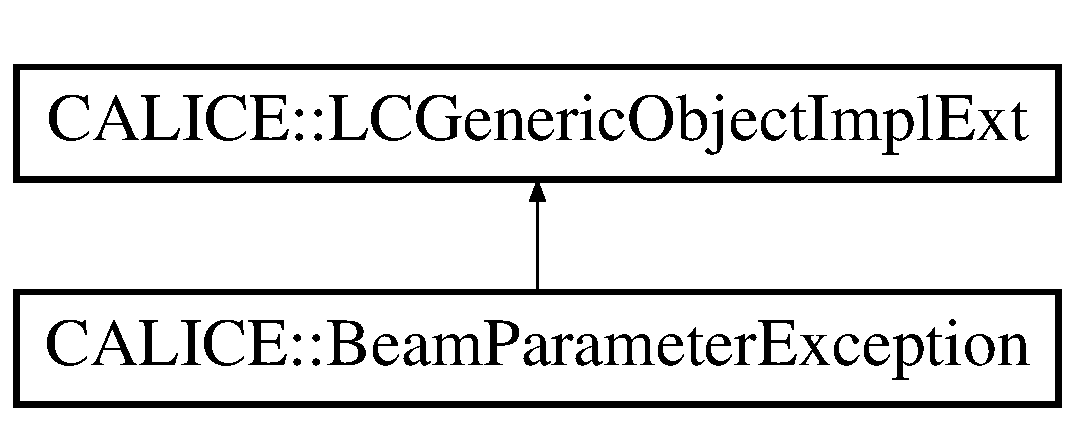
\includegraphics[height=2cm]{classCALICE_1_1BeamParameterException}
\end{center}
\end{figure}
\subsection*{Public Member Functions}
\begin{DoxyCompactItemize}
\item 
{\bf BeamParameterException} (LCObject $\ast$obj)\label{classCALICE_1_1BeamParameterException_a8ae0f2f91f0d1a8d757cfafc6f9040b7}

\begin{DoxyCompactList}\small\item\em 'Copy constructor' needed to interpret LCCollection read from file/database. \item\end{DoxyCompactList}\item 
{\bf BeamParameterException} \& {\bf setBeamEnergy} (unsigned int energy)
\begin{DoxyCompactList}\small\item\em Set the particle type. \item\end{DoxyCompactList}\item 
unsigned int {\bf getBeamEnergy} () const \label{classCALICE_1_1BeamParameterException_a207e7eed23b2eb26389e20af3a4a4d6d}

\begin{DoxyCompactList}\small\item\em Get the maximum of the beam energy distribution. \item\end{DoxyCompactList}\item 
void {\bf print} (std::ostream \&os)\label{classCALICE_1_1BeamParameterException_ad198507745bc2607d95f62d671f3ae56}

\begin{DoxyCompactList}\small\item\em Print all members (for debugging). \item\end{DoxyCompactList}\item 
const std::string {\bf getTypeName} () const \label{classCALICE_1_1BeamParameterException_a03e95b25675a8b394ae4e75781c52a46}

\begin{DoxyCompactList}\small\item\em Return the type of the class. \item\end{DoxyCompactList}\item 
const std::string {\bf getDataDescription} () const \label{classCALICE_1_1BeamParameterException_ad3e64e3f1fa0fabe6689639f0a2f6c68}

\begin{DoxyCompactList}\small\item\em Return a brief description of the data members. \item\end{DoxyCompactList}\end{DoxyCompactItemize}


\subsection{Detailed Description}
This class handles beam parameters which have been written by hand into the database. It is to be used if beam parameters are either not available at all or if the analysis of the r/o has revealed some odds. This class might evolve with time, for the time being it constains only the beam energy. \begin{DoxyAuthor}{Author}
R. P�schl LAL 
\end{DoxyAuthor}
\begin{DoxyDate}{Date}
Oct 2007 
\end{DoxyDate}


Definition at line 28 of file BeamParameterException.hh.

\subsection{Member Function Documentation}
\index{CALICE::BeamParameterException@{CALICE::BeamParameterException}!setBeamEnergy@{setBeamEnergy}}
\index{setBeamEnergy@{setBeamEnergy}!CALICE::BeamParameterException@{CALICE::BeamParameterException}}
\subsubsection[{setBeamEnergy}]{\setlength{\rightskip}{0pt plus 5cm}{\bf BeamParameterException}\& CALICE::BeamParameterException::setBeamEnergy (unsigned int {\em energy})\hspace{0.3cm}{\ttfamily  [inline]}}\label{classCALICE_1_1BeamParameterException_a157244f293c4ee00795aec9992e3771e}


Set the particle type. Get the particle type. Return the beam type name for a given type id. Return the beam type name. Set the nominal beam energy. 

Definition at line 65 of file BeamParameterException.hh.

References CALICE::kBeamParameterExceptionIntBeamEnergy, and CALICE::LCGenericObjectImplExt::obj().

The documentation for this class was generated from the following files:\begin{DoxyCompactItemize}
\item 
BeamParameterException.hh\item 
BeamParameterException.cc\end{DoxyCompactItemize}

\section{CALICE::BeEvent Class Reference}
\label{classCALICE_1_1BeEvent}\index{CALICE::BeEvent@{CALICE::BeEvent}}


Stores the trigger history (i.e.  


{\ttfamily \#include $<$BeEvent.hh$>$}Inheritance diagram for CALICE::BeEvent::\begin{figure}[H]
\begin{center}
\leavevmode
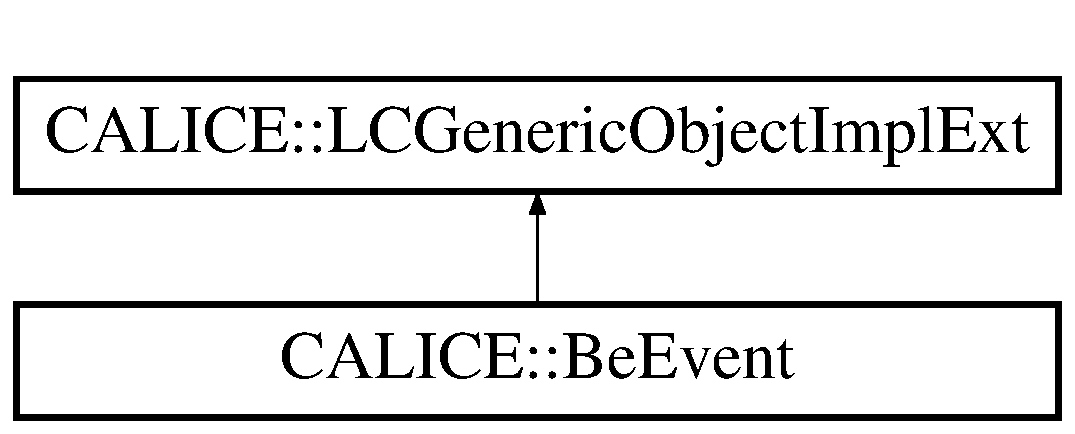
\includegraphics[height=2cm]{classCALICE_1_1BeEvent}
\end{center}
\end{figure}
\subsection*{Public Member Functions}
\begin{DoxyCompactItemize}
\item 
{\bf BeEvent} ()\label{classCALICE_1_1BeEvent_a2097c6cad17364e073130b88759d4395}

\begin{DoxyCompactList}\small\item\em Simple Constructor. \item\end{DoxyCompactList}\item 
{\bf BeEvent} (unsigned int board\_\-id)
\begin{DoxyCompactList}\small\item\em UsefulConstructor. \item\end{DoxyCompactList}\item 
{\bf BeEvent} (LCObject $\ast$obj)\label{classCALICE_1_1BeEvent_aa434832dc8f050ab7d92ea2a90e3a2fa}

\begin{DoxyCompactList}\small\item\em 'Copy constructor' needed to interpret LCCollection read from file/database. \item\end{DoxyCompactList}\item 
{\bf BeEvent} \& {\bf setBoardID} (int boardID)
\begin{DoxyCompactList}\small\item\em Set the packed board id. \item\end{DoxyCompactList}\item 
int {\bf getBoardID} () const \label{classCALICE_1_1BeEvent_a257d5c382c76e453d576c99b4785811d}

\begin{DoxyCompactList}\small\item\em Get the board id. \item\end{DoxyCompactList}\item 
{\bf BeEvent} \& {\bf setRecordLabel} (int label)\label{classCALICE_1_1BeEvent_ab860bbf02c55df7b26c2e9335056a21a}

\begin{DoxyCompactList}\small\item\em Set the Record Label. \item\end{DoxyCompactList}\item 
short {\bf getRecordLabel} () const \label{classCALICE_1_1BeEvent_a9cc54e7581f285b926a192836e904e86}

\begin{DoxyCompactList}\small\item\em Return the Record Label. \item\end{DoxyCompactList}\item 
{\bf BeEvent} \& {\bf setStatusWord} (int status)\label{classCALICE_1_1BeEvent_a052f9cb87c190b8137d6ad09e676af1f}

\begin{DoxyCompactList}\small\item\em Set the status word. \item\end{DoxyCompactList}\item 
int {\bf getStatusWord} () const \label{classCALICE_1_1BeEvent_afffb8609964ae7e46d4eb7c55d6cac08}

\begin{DoxyCompactList}\small\item\em Get the status word. \item\end{DoxyCompactList}\item 
{\bf BeEvent} \& {\bf setL1aCounter} (int l1acounter)\label{classCALICE_1_1BeEvent_ad4dec434b6ae2f78e9db131d26b6330f}

\begin{DoxyCompactList}\small\item\em Set the l1acounter This number is used to check integrity of trigger counters. \item\end{DoxyCompactList}\item 
int {\bf getL1aCounter} () const \label{classCALICE_1_1BeEvent_a3bb48d738f07c16324f75e5f3f6594d6}

\begin{DoxyCompactList}\small\item\em Get the l1acounter. \item\end{DoxyCompactList}\item 
{\bf BeEvent} \& {\bf setBxCounter} (int bxcount)\label{classCALICE_1_1BeEvent_a94fe845cc1ced1dc5743f784f6092bfa}

\begin{DoxyCompactList}\small\item\em Set the bxcounter (bunch crossing !?). \item\end{DoxyCompactList}\item 
int {\bf getBxCounter} () const \label{classCALICE_1_1BeEvent_a85aad5b07a8644221039c50f47c9cfe2}

\begin{DoxyCompactList}\small\item\em Get the bxcounter. \item\end{DoxyCompactList}\item 
{\bf BeEvent} \& {\bf setQdrFrameCounter} (int qdrframecount)
\begin{DoxyCompactList}\small\item\em Set the QdrFrameCounter (Whatever this is . \item\end{DoxyCompactList}\item 
int {\bf getQdrFrameCounter} () const \label{classCALICE_1_1BeEvent_aef1af66fdeecc7b3e78b6e164681341a}

\begin{DoxyCompactList}\small\item\em Get the QdrFrameCounter. \item\end{DoxyCompactList}\item 
{\bf BeEvent} \& {\bf setQdrDataCounter} (int qdrdatacount)
\begin{DoxyCompactList}\small\item\em Set the QdrDataCounter (Whatever this is . \item\end{DoxyCompactList}\item 
int {\bf getQdrDataCounter} () const \label{classCALICE_1_1BeEvent_ad917495373bd3b1f6261f0043aca87e0}

\begin{DoxyCompactList}\small\item\em Get the QdrDataCounter. \item\end{DoxyCompactList}\item 
{\bf BeEvent} \& {\bf setTotalFrameCounter} (int totalframecount)
\begin{DoxyCompactList}\small\item\em Set the TotalFrameCounter (Whatever this is . \item\end{DoxyCompactList}\item 
int {\bf getTotalFrameCounter} () const \label{classCALICE_1_1BeEvent_afbe2088acfa3d8d5a4301d66c9bec655}

\begin{DoxyCompactList}\small\item\em Get the TotalFrameCounter. \item\end{DoxyCompactList}\item 
void {\bf print} (std::ostream \&os)\label{classCALICE_1_1BeEvent_a9554fd6824f75d8bfbfa3183ba8469b1}

\begin{DoxyCompactList}\small\item\em Convenient print method. \item\end{DoxyCompactList}\item 
const std::string {\bfseries getTypeName} () const \label{classCALICE_1_1BeEvent_a1a9609c2a147fa44055bc3aae63d64c6}

\item 
const std::string {\bf getDataDescription} () const \label{classCALICE_1_1BeEvent_a271ed21e4fc8b27bffd8ba9cf3c7d31b}

\begin{DoxyCompactList}\small\item\em Return a brief description of the data members. \item\end{DoxyCompactList}\end{DoxyCompactItemize}


\subsection{Detailed Description}
Stores the trigger history (i.e. fifo content).when it appears in the front end as realized for runs starting in May 2006 (Ask Paul for firmware version) in older versions of the DAQ these data came along wiith the BeTrgEventData which still contains information related to the data handled by the present interface class.

To acces the configuration: 
\begin{DoxyPre}
   void processEvent(LCEvent *event)  \{
       try \{
        // string \_colName = "BeTrgEventData"
        LCCollection *col=event->getCollection(\_colName);
        for (unsigned int element\_i=0; element\_i<col->getNumberOfElements(); element\_i++) \{
           \doxyref{BeEvent}{p.}{classCALICE_1_1BeEvent} event(col->getElementAt(element\_i));\end{DoxyPre}



\begin{DoxyPre}        \}
   \}
 \end{DoxyPre}


\begin{DoxyAuthor}{Author}
R. P�schl (LAL Orsay) 
\end{DoxyAuthor}
\begin{DoxyDate}{Date}
Jul 2006 
\end{DoxyDate}


Definition at line 58 of file BeEvent.hh.

\subsection{Constructor \& Destructor Documentation}
\index{CALICE::BeEvent@{CALICE::BeEvent}!BeEvent@{BeEvent}}
\index{BeEvent@{BeEvent}!CALICE::BeEvent@{CALICE::BeEvent}}
\subsubsection[{BeEvent}]{\setlength{\rightskip}{0pt plus 5cm}CALICE::BeEvent::BeEvent (unsigned int {\em board\_\-id})\hspace{0.3cm}{\ttfamily  [inline]}}\label{classCALICE_1_1BeEvent_a52f929c3fccdded286f6bfb5f3989f09}


UsefulConstructor. 
\begin{DoxyParams}{Parameters}
\item[{\em board\_\-id}]the packed board id (\doxyref{CALICE::BoardID}{p.}{classCALICE_1_1BoardID}). \end{DoxyParams}


Definition at line 80 of file BeEvent.hh.

References setBoardID(), setBxCounter(), setL1aCounter(), setQdrDataCounter(), setQdrFrameCounter(), setRecordLabel(), setStatusWord(), and setTotalFrameCounter().

\subsection{Member Function Documentation}
\index{CALICE::BeEvent@{CALICE::BeEvent}!setBoardID@{setBoardID}}
\index{setBoardID@{setBoardID}!CALICE::BeEvent@{CALICE::BeEvent}}
\subsubsection[{setBoardID}]{\setlength{\rightskip}{0pt plus 5cm}{\bf BeEvent}\& CALICE::BeEvent::setBoardID (int {\em boardID})\hspace{0.3cm}{\ttfamily  [inline]}}\label{classCALICE_1_1BeEvent_a63f17cd05b53cb5c3ec91432c54b8ccc}


Set the packed board id. \begin{DoxySeeAlso}{See also}
\doxyref{BoardID}{p.}{classCALICE_1_1BoardID} 
\end{DoxySeeAlso}


Definition at line 108 of file BeEvent.hh.

References CALICE::LCGenericObjectImplExt::obj().

Referenced by BeEvent().\index{CALICE::BeEvent@{CALICE::BeEvent}!setQdrDataCounter@{setQdrDataCounter}}
\index{setQdrDataCounter@{setQdrDataCounter}!CALICE::BeEvent@{CALICE::BeEvent}}
\subsubsection[{setQdrDataCounter}]{\setlength{\rightskip}{0pt plus 5cm}{\bf BeEvent}\& CALICE::BeEvent::setQdrDataCounter (int {\em qdrdatacount})\hspace{0.3cm}{\ttfamily  [inline]}}\label{classCALICE_1_1BeEvent_ad085e6f2c86bfc12a9c450f55f6a65f6}


Set the QdrDataCounter (Whatever this is . ..) 

Definition at line 163 of file BeEvent.hh.

References CALICE::LCGenericObjectImplExt::obj().

Referenced by BeEvent().\index{CALICE::BeEvent@{CALICE::BeEvent}!setQdrFrameCounter@{setQdrFrameCounter}}
\index{setQdrFrameCounter@{setQdrFrameCounter}!CALICE::BeEvent@{CALICE::BeEvent}}
\subsubsection[{setQdrFrameCounter}]{\setlength{\rightskip}{0pt plus 5cm}{\bf BeEvent}\& CALICE::BeEvent::setQdrFrameCounter (int {\em qdrframecount})\hspace{0.3cm}{\ttfamily  [inline]}}\label{classCALICE_1_1BeEvent_abd097e21aaa8d7ac65f473186ec0ec6a}


Set the QdrFrameCounter (Whatever this is . ..) 

Definition at line 155 of file BeEvent.hh.

References CALICE::LCGenericObjectImplExt::obj().

Referenced by BeEvent().\index{CALICE::BeEvent@{CALICE::BeEvent}!setTotalFrameCounter@{setTotalFrameCounter}}
\index{setTotalFrameCounter@{setTotalFrameCounter}!CALICE::BeEvent@{CALICE::BeEvent}}
\subsubsection[{setTotalFrameCounter}]{\setlength{\rightskip}{0pt plus 5cm}{\bf BeEvent}\& CALICE::BeEvent::setTotalFrameCounter (int {\em totalframecount})\hspace{0.3cm}{\ttfamily  [inline]}}\label{classCALICE_1_1BeEvent_accec6ea69ebb86a919ea63115ef9ee90}


Set the TotalFrameCounter (Whatever this is . ..) 

Definition at line 171 of file BeEvent.hh.

References CALICE::LCGenericObjectImplExt::obj().

Referenced by BeEvent().

The documentation for this class was generated from the following file:\begin{DoxyCompactItemize}
\item 
BeEvent.hh\end{DoxyCompactItemize}

\section{CALICE::BeTrgConf Class Reference}
\label{classCALICE_1_1BeTrgConf}\index{CALICE::BeTrgConf@{CALICE::BeTrgConf}}


Stores the configuration data of the trigger.  


{\ttfamily \#include $<$BeTrgConf.hh$>$}Inheritance diagram for CALICE::BeTrgConf::\begin{figure}[H]
\begin{center}
\leavevmode
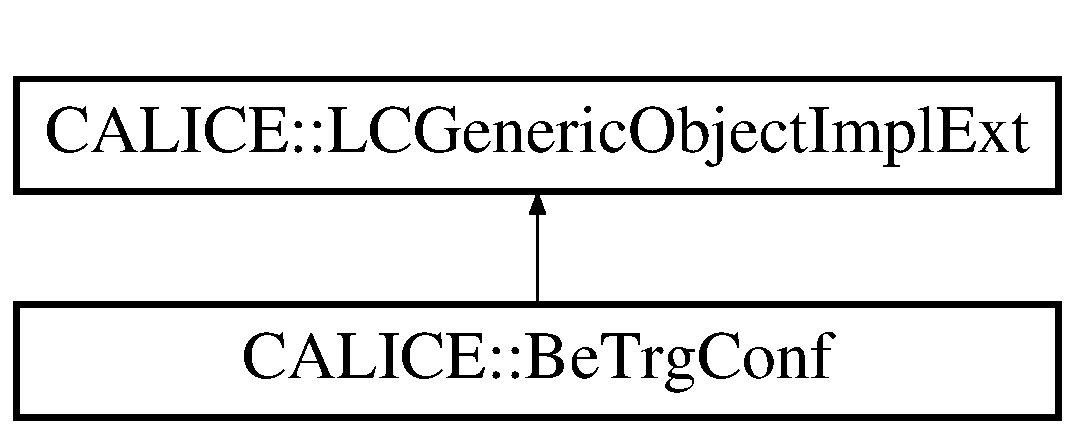
\includegraphics[height=2cm]{classCALICE_1_1BeTrgConf}
\end{center}
\end{figure}
\subsection*{Public Member Functions}
\begin{DoxyCompactItemize}
\item 
{\bf BeTrgConf} ()\label{classCALICE_1_1BeTrgConf_a8c09539bda8db3784aae4fbcbcb0ec3f}

\begin{DoxyCompactList}\small\item\em Default Constructor. \item\end{DoxyCompactList}\item 
{\bf BeTrgConf} (int boardID)
\begin{DoxyCompactList}\small\item\em Ctor. \item\end{DoxyCompactList}\item 
{\bf BeTrgConf} (LCObject $\ast$obj)\label{classCALICE_1_1BeTrgConf_aa6bbe7ee49bfb432a38a8425fddd3c45}

\begin{DoxyCompactList}\small\item\em 'Copy constructor' needed to interpret LCCollection read from file/database. \item\end{DoxyCompactList}\item 
{\bf BeTrgConf} \& {\bf setBoardID} (int boardID)
\begin{DoxyCompactList}\small\item\em set the packed board id. \item\end{DoxyCompactList}\item 
int {\bf getBoardID} () const \label{classCALICE_1_1BeTrgConf_a332e453076685a181fc82b50782a89f2}

\begin{DoxyCompactList}\small\item\em Information on the FE chip the data was received. \item\end{DoxyCompactList}\item 
void {\bf setRecordLabel} (int label)\label{classCALICE_1_1BeTrgConf_a75c2b5f2bdf803500688e0e427545ac5}

\begin{DoxyCompactList}\small\item\em Set the Record Label. \item\end{DoxyCompactList}\item 
short {\bf getRecordLabel} () const \label{classCALICE_1_1BeTrgConf_a3a35836bbb8aa32bcba88d0bbbed2686}

\begin{DoxyCompactList}\small\item\em Return the Record Label. \item\end{DoxyCompactList}\item 
{\bf BeTrgConf} \& {\bf setInputEnableMask} (int input\_\-enable)
\begin{DoxyCompactList}\small\item\em Set the trigger enable bit mask. \item\end{DoxyCompactList}\item 
int {\bf getInputEnableMask} () const 
\begin{DoxyCompactList}\small\item\em Get the trigger enable bit mask. \item\end{DoxyCompactList}\item 
{\bf BeTrgConf} \& {\bf setOscillatorEnable} (int osc\_\-enable)\label{classCALICE_1_1BeTrgConf_ac5c442bfe4a6d5d8da543c5444453491}

\begin{DoxyCompactList}\small\item\em Set Oscillator Enable. \item\end{DoxyCompactList}\item 
int {\bf getOscillatorEnable} () const \label{classCALICE_1_1BeTrgConf_a786f6d987d88cfff6be350d8d2da72b6}

\begin{DoxyCompactList}\small\item\em Get Oscillator Enable. \item\end{DoxyCompactList}\item 
{\bf BeTrgConf} \& {\bf setGeneralEnable} (int gen\_\-enable)\label{classCALICE_1_1BeTrgConf_a0ec05d6c7bcff2ba528ecbfd3ba02c1e}

\begin{DoxyCompactList}\small\item\em Set General Enable. \item\end{DoxyCompactList}\item 
int {\bf getGeneralEnable} () const \label{classCALICE_1_1BeTrgConf_a4c4a9313bba8a0ed7f81092c8f6f1fec}

\begin{DoxyCompactList}\small\item\em Get General Enable. \item\end{DoxyCompactList}\item 
{\bf BeTrgConf} \& {\bf setOscillationPeriod} (int oscillation\_\-period)\label{classCALICE_1_1BeTrgConf_a03be1fd0409f19b3bf6b237a4b551e4e}

\begin{DoxyCompactList}\small\item\em Set the oscillation period. \item\end{DoxyCompactList}\item 
int {\bf getOscillationPeriod} () const \label{classCALICE_1_1BeTrgConf_ac84ad8d502d2306e9380666a870c60ae}

\begin{DoxyCompactList}\small\item\em Get the oscillation period. \item\end{DoxyCompactList}\item 
{\bf BeTrgConf} \& {\bf setBurstCounter} (int burst\_\-count)\label{classCALICE_1_1BeTrgConf_a9ffc7c295209cf416ed76e3e161f5ad2}

\begin{DoxyCompactList}\small\item\em Set the burst counter. \item\end{DoxyCompactList}\item 
int {\bf getBurstCounter} () const \label{classCALICE_1_1BeTrgConf_af28d7356fda3f116f34dabd50d52f798}

\begin{DoxyCompactList}\small\item\em Get the burst counter. \item\end{DoxyCompactList}\item 
{\bf BeTrgConf} \& {\bf setConfiguration} (int config)\label{classCALICE_1_1BeTrgConf_acec95f60250ce4a5d42f9aa7e58db7a7}

\begin{DoxyCompactList}\small\item\em Set the configuration word. \item\end{DoxyCompactList}\item 
int {\bf getConfiguration} () const \label{classCALICE_1_1BeTrgConf_a4da9e0491cd18b711e110fc90cabbd57}

\begin{DoxyCompactList}\small\item\em Get the configuration word. \item\end{DoxyCompactList}\item 
{\bf BeTrgConf} \& {\bf setFifoIdleDepth} (int fifo\_\-idle\_\-depth)\label{classCALICE_1_1BeTrgConf_ac8baef28684cbcd0a2ffcf4238262d78}

\begin{DoxyCompactList}\small\item\em Set the fifo idle depth. \item\end{DoxyCompactList}\item 
int {\bf getFifoIdleDepth} () const \label{classCALICE_1_1BeTrgConf_a2285119c2c7c779f80cfade5ddbd6873}

\begin{DoxyCompactList}\small\item\em Get the fifo idle depth. \item\end{DoxyCompactList}\item 
{\bf BeTrgConf} \& {\bf setBusyTimeout} (int busy\_\-timeout)\label{classCALICE_1_1BeTrgConf_ac4796b32d11183db7c4c26cc27068b04}

\begin{DoxyCompactList}\small\item\em Set the busy time out. \item\end{DoxyCompactList}\item 
int {\bf getBusyTimeout} () const \label{classCALICE_1_1BeTrgConf_a92ccb523a8c71cbd92bdd2377120331a}

\begin{DoxyCompactList}\small\item\em Get the busy time out. \item\end{DoxyCompactList}\item 
{\bf BeTrgConf} \& {\bf setBurstTimeout} (int burst\_\-timeout)\label{classCALICE_1_1BeTrgConf_ad1fd90e88ae2d537566b7626fe20f91b}

\begin{DoxyCompactList}\small\item\em Set the burst time out. \item\end{DoxyCompactList}\item 
int {\bf getBurstTimeout} () const \label{classCALICE_1_1BeTrgConf_ab7dc9b50b96c180c995e16a0a264acdb}

\begin{DoxyCompactList}\small\item\em Get the burst time out. \item\end{DoxyCompactList}\item 
{\bf BeTrgConf} \& {\bf setAndEnable} (int and\_\-enable, int pos)\label{classCALICE_1_1BeTrgConf_a3030bed7c53e0be53ffe16ade5551c8b}

\begin{DoxyCompactList}\small\item\em Set the andEnable. \item\end{DoxyCompactList}\item 
int {\bf getAndEnable} (int pos) const \label{classCALICE_1_1BeTrgConf_a5eff0a3b3e4cc9d68b1de91fd91ed519}

\begin{DoxyCompactList}\small\item\em Get the and Enable. \item\end{DoxyCompactList}\item 
{\bf BeTrgConf} \& {\bf setExtBeamMode} (int ext\_\-beammode)\label{classCALICE_1_1BeTrgConf_a2d67e0ec00b152680779250acccb556b}

\begin{DoxyCompactList}\small\item\em Set the extBeam Mode. \item\end{DoxyCompactList}\item 
int {\bf getExtBeamMode} () const \label{classCALICE_1_1BeTrgConf_a3c292917f3b29f5ef1a771ad8f1f4f7b}

\begin{DoxyCompactList}\small\item\em Get the extBeam Mode. \item\end{DoxyCompactList}\item 
{\bf BeTrgConf} \& {\bf setInputInvert} (int input\_\-invert)\label{classCALICE_1_1BeTrgConf_aada94ccc553d5cda4b6cf1a2cf173601}

\begin{DoxyCompactList}\small\item\em Set the input invert. \item\end{DoxyCompactList}\item 
int {\bf getInputInvert} () const \label{classCALICE_1_1BeTrgConf_a3b4aeee59a32fda0efa23fcfa3327f77}

\begin{DoxyCompactList}\small\item\em Get the input invert. \item\end{DoxyCompactList}\item 
{\bf BeTrgConf} \& {\bf setQdrConfiguration} (int qdr\_\-config)\label{classCALICE_1_1BeTrgConf_a9b707b4d34d920e835988e48ded4cc37}

\begin{DoxyCompactList}\small\item\em Set the qdr configuration. \item\end{DoxyCompactList}\item 
int {\bf getQdrConfiguration} () const \label{classCALICE_1_1BeTrgConf_a8879baa5b1fc4d073b11d6b065a73e7d}

\begin{DoxyCompactList}\small\item\em Get the qdr configuration. \item\end{DoxyCompactList}\item 
{\bf BeTrgConf} \& {\bf setSequencerControl} (int sequence\_\-contr)\label{classCALICE_1_1BeTrgConf_a4583754d7a4cf65c1fb86d29ea836cac}

\begin{DoxyCompactList}\small\item\em Set the sequencer control. \item\end{DoxyCompactList}\item 
int {\bf getSequencerControl} () const \label{classCALICE_1_1BeTrgConf_adb6f6981514a038e70c2e479240fdb3f}

\begin{DoxyCompactList}\small\item\em Get the sequencer control. \item\end{DoxyCompactList}\item 
void {\bf print} (std::ostream \&os)\label{classCALICE_1_1BeTrgConf_a986684df66d456e9275f711d59c913ed}

\begin{DoxyCompactList}\small\item\em Convenient print method. \item\end{DoxyCompactList}\item 
const std::string {\bf getTypeName} () const \label{classCALICE_1_1BeTrgConf_ab51e1dcd328cea0821792d00e49ef504}

\begin{DoxyCompactList}\small\item\em Return the type of the class. \item\end{DoxyCompactList}\item 
const std::string {\bf getDataDescription} () const \label{classCALICE_1_1BeTrgConf_a396979e8da1cf0d9e19930e75fd8c858}

\begin{DoxyCompactList}\small\item\em Return a brief description of the data members. \item\end{DoxyCompactList}\end{DoxyCompactItemize}


\subsection{Detailed Description}
Stores the configuration data of the trigger. To acces the configuration: 
\begin{DoxyPre}
   void BrTrgCondChangeListener(LCCollection *col)  \{
        assert (col->getNumberOfElements()==1)
        \doxyref{BeTrgConf}{p.}{classCALICE_1_1BeTrgConf} conf(col->getElementAt(0));\end{DoxyPre}



\begin{DoxyPre}        UInt\_t enable\_mask=conf.getEnableMask();
   \}
 \end{DoxyPre}


\begin{DoxySeeAlso}{See also}
\doxyref{ConditionsChangeDelegator}{p.}{classCALICE_1_1ConditionsChangeDelegator} 
\end{DoxySeeAlso}
\begin{DoxyAuthor}{Author}
G�tz Gaycken LLR (Ecole Polytechnique) 
\end{DoxyAuthor}
\begin{DoxyDate}{Date}
Sep 2005 
\end{DoxyDate}


Definition at line 76 of file BeTrgConf.hh.

\subsection{Constructor \& Destructor Documentation}
\index{CALICE::BeTrgConf@{CALICE::BeTrgConf}!BeTrgConf@{BeTrgConf}}
\index{BeTrgConf@{BeTrgConf}!CALICE::BeTrgConf@{CALICE::BeTrgConf}}
\subsubsection[{BeTrgConf}]{\setlength{\rightskip}{0pt plus 5cm}CALICE::BeTrgConf::BeTrgConf (int {\em boardID})\hspace{0.3cm}{\ttfamily  [inline]}}\label{classCALICE_1_1BeTrgConf_a5af9732e0e1783bfc26a513911e9d85e}


Ctor. 
\begin{DoxyParams}{Parameters}
\item[{\em boardID}]the packed board id (\doxyref{BoardID}{p.}{classCALICE_1_1BoardID}). \end{DoxyParams}


Definition at line 86 of file BeTrgConf.hh.

References CALICE::LCGenericObjectImplExt::obj().

\subsection{Member Function Documentation}
\index{CALICE::BeTrgConf@{CALICE::BeTrgConf}!getInputEnableMask@{getInputEnableMask}}
\index{getInputEnableMask@{getInputEnableMask}!CALICE::BeTrgConf@{CALICE::BeTrgConf}}
\subsubsection[{getInputEnableMask}]{\setlength{\rightskip}{0pt plus 5cm}int CALICE::BeTrgConf::getInputEnableMask () const\hspace{0.3cm}{\ttfamily  [inline]}}\label{classCALICE_1_1BeTrgConf_ac38488bad25a502a3b0c15d0b5030efc}


Get the trigger enable bit mask. For each aenabled trigger a bit is set. The meaning of the bits is defined by conditions data. \begin{DoxySeeAlso}{See also}
TriggerMask. 
\end{DoxySeeAlso}


Definition at line 128 of file BeTrgConf.hh.

Referenced by print().\index{CALICE::BeTrgConf@{CALICE::BeTrgConf}!setBoardID@{setBoardID}}
\index{setBoardID@{setBoardID}!CALICE::BeTrgConf@{CALICE::BeTrgConf}}
\subsubsection[{setBoardID}]{\setlength{\rightskip}{0pt plus 5cm}{\bf BeTrgConf}\& CALICE::BeTrgConf::setBoardID (int {\em boardID})\hspace{0.3cm}{\ttfamily  [inline]}}\label{classCALICE_1_1BeTrgConf_aebabae2847b682da59cb5e2f5ec15141}


set the packed board id. \begin{DoxySeeAlso}{See also}
\doxyref{BoardID}{p.}{classCALICE_1_1BoardID} 
\end{DoxySeeAlso}


Definition at line 97 of file BeTrgConf.hh.

References CALICE::LCGenericObjectImplExt::obj().\index{CALICE::BeTrgConf@{CALICE::BeTrgConf}!setInputEnableMask@{setInputEnableMask}}
\index{setInputEnableMask@{setInputEnableMask}!CALICE::BeTrgConf@{CALICE::BeTrgConf}}
\subsubsection[{setInputEnableMask}]{\setlength{\rightskip}{0pt plus 5cm}{\bf BeTrgConf}\& CALICE::BeTrgConf::setInputEnableMask (int {\em input\_\-enable})\hspace{0.3cm}{\ttfamily  [inline]}}\label{classCALICE_1_1BeTrgConf_a4adeeec5eb99fe7b5bba2e12cb525c38}


Set the trigger enable bit mask. For each aenabled trigger a bit is set. The meaning of the bits is defined by conditions data. \begin{DoxySeeAlso}{See also}
TriggerMask. 
\end{DoxySeeAlso}


Definition at line 118 of file BeTrgConf.hh.

References CALICE::LCGenericObjectImplExt::obj().

The documentation for this class was generated from the following file:\begin{DoxyCompactItemize}
\item 
BeTrgConf.hh\end{DoxyCompactItemize}

\section{CALICE::BeTrgEvent Class Reference}
\label{classCALICE_1_1BeTrgEvent}\index{CALICE::BeTrgEvent@{CALICE::BeTrgEvent}}


Stores the trigger event data.  


{\ttfamily \#include $<$BeTrgEvent.hh$>$}Inheritance diagram for CALICE::BeTrgEvent::\begin{figure}[H]
\begin{center}
\leavevmode
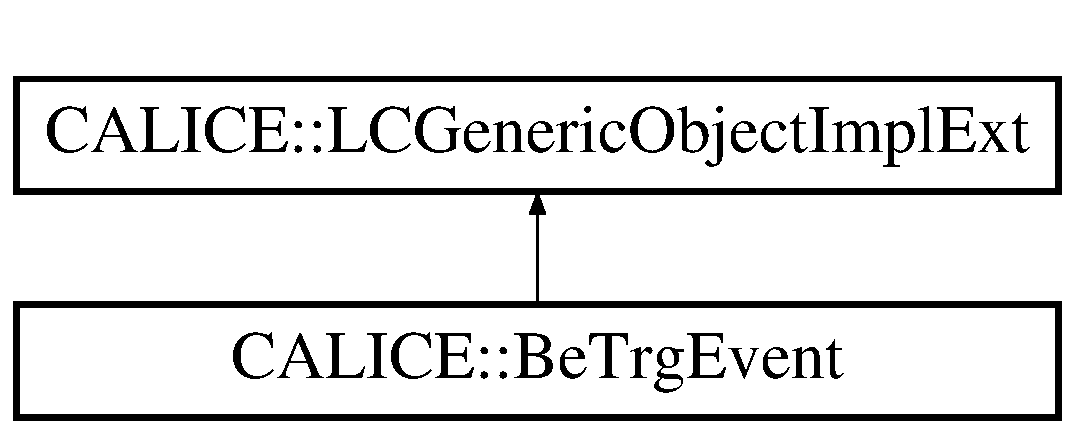
\includegraphics[height=2cm]{classCALICE_1_1BeTrgEvent}
\end{center}
\end{figure}
\subsection*{Public Member Functions}
\begin{DoxyCompactItemize}
\item 
{\bf BeTrgEvent} (unsigned int board\_\-id)
\begin{DoxyCompactList}\small\item\em UsefulConstructor. \item\end{DoxyCompactList}\item 
{\bf BeTrgEvent} (LCObject $\ast$obj)\label{classCALICE_1_1BeTrgEvent_aad3ab901206f9cfe9867505455e014fe}

\begin{DoxyCompactList}\small\item\em 'Copy constructor' needed to interpret LCCollection read from file/database. \item\end{DoxyCompactList}\item 
{\bf BeTrgEvent} \& {\bf setBoardID} (int boardID)
\begin{DoxyCompactList}\small\item\em set the packed board id. \item\end{DoxyCompactList}\item 
int {\bf getBoardID} () const \label{classCALICE_1_1BeTrgEvent_a0a62c75cb07342d47e5298ebfb34f7d8}

\begin{DoxyCompactList}\small\item\em Information on the FE chip the data was received. \item\end{DoxyCompactList}\item 
{\bf BeTrgEvent} \& {\bf setInputStatus} (int input\_\-status)
\begin{DoxyCompactList}\small\item\em Set the pre busy trigger counter (what ever that is ;-\/). \item\end{DoxyCompactList}\item 
int {\bf getInputStatus} () const \label{classCALICE_1_1BeTrgEvent_acaea9fd53c2fd11f7b31db9ea9806658}

\begin{DoxyCompactList}\small\item\em Get the input status. \item\end{DoxyCompactList}\item 
{\bf BeTrgEvent} \& {\bf setInputCatch} (int input\_\-catch)\label{classCALICE_1_1BeTrgEvent_af1b27f8a852855d164e5f71b7406998c}

\begin{DoxyCompactList}\small\item\em Set the input catch (what ever that is ;-\/). \item\end{DoxyCompactList}\item 
int {\bf getInputCatch} () const \label{classCALICE_1_1BeTrgEvent_ae076fd16cf3ee806c64a1d2e82e29f50}

\begin{DoxyCompactList}\small\item\em Get the input catch (what ever that is ;-\/). \item\end{DoxyCompactList}\item 
{\bf BeTrgEvent} \& {\bf setPreBusyCatch} (int prebusy\_\-catch)
\begin{DoxyCompactList}\small\item\em Set the trigger busy status. \item\end{DoxyCompactList}\item 
int {\bf getPrebusyCatch} () const \label{classCALICE_1_1BeTrgEvent_a06df76683895a30404a54912b09d210a}

\begin{DoxyCompactList}\small\item\em Get the prebusy Catch. \item\end{DoxyCompactList}\item 
{\bf BeTrgEvent} \& {\bf setSignalCatch} (int signal\_\-catch)\label{classCALICE_1_1BeTrgEvent_a8cf5425520f7881a57cb36a959fc256f}

\begin{DoxyCompactList}\small\item\em Set the signal Catch. \item\end{DoxyCompactList}\item 
int {\bf getSignalCatch} () const \label{classCALICE_1_1BeTrgEvent_a0afe03ca2e64566c074045563fb62ef9}

\begin{DoxyCompactList}\small\item\em Get the signal Catch. \item\end{DoxyCompactList}\item 
{\bf BeTrgEvent} \& {\bf setControl} (int control)\label{classCALICE_1_1BeTrgEvent_a145c2a82f590cd2350a1f6c5d350c178}

\begin{DoxyCompactList}\small\item\em Set the contrl value. \item\end{DoxyCompactList}\item 
int {\bf getControl} () const \label{classCALICE_1_1BeTrgEvent_acf9e7facc723fe1c420b3cd2c1b4993f}

\begin{DoxyCompactList}\small\item\em Get the control value. \item\end{DoxyCompactList}\item 
{\bf BeTrgEvent} \& {\bf setInitialFifoStatus} (int initial\_\-fifo\_\-status)\label{classCALICE_1_1BeTrgEvent_ae2c3ed9c3ebfd484ea022bb308a6faca}

\begin{DoxyCompactList}\small\item\em Set the inital fifo status. \item\end{DoxyCompactList}\item 
int {\bf getInitialFifoStatus} () const \label{classCALICE_1_1BeTrgEvent_a4359fbafae59cc303c5160f3626c74e6}

\begin{DoxyCompactList}\small\item\em Get the initial fifo status. \item\end{DoxyCompactList}\item 
{\bf BeTrgEvent} \& {\bf setFinalFifoStatus} (int final\_\-fifo\_\-status)\label{classCALICE_1_1BeTrgEvent_aef331b17a4eca0f054c3379b517c1bbe}

\begin{DoxyCompactList}\small\item\em Set the final fifo status. \item\end{DoxyCompactList}\item 
int {\bf getFinalFifoStatus} () const \label{classCALICE_1_1BeTrgEvent_a7674994d84b63ae049e64fbbae486289}

\begin{DoxyCompactList}\small\item\em Get the final fifo status. \item\end{DoxyCompactList}\item 
{\bf BeTrgEvent} \& {\bf setFifoWord} (unsigned int word\_\-index, unsigned int word)
\begin{DoxyCompactList}\small\item\em Set the fifo word. \item\end{DoxyCompactList}\item 
{\bf BeTrgEvent} \& {\bf setAllFifoWords} (unsigned int n\_\-words, const unsigned int $\ast$const word\_\-list)
\begin{DoxyCompactList}\small\item\em Set all the fifo words. \item\end{DoxyCompactList}\item 
int {\bf getNFifoWords} () const \label{classCALICE_1_1BeTrgEvent_a8dad5638340b3046d0cad0012fe1c03a}

\begin{DoxyCompactList}\small\item\em Get the number of words contained in the fifo. \item\end{DoxyCompactList}\item 
int {\bf getFifoWord} (unsigned int word\_\-index) const 
\begin{DoxyCompactList}\small\item\em Get a fifo word. \item\end{DoxyCompactList}\item 
IntVec \& {\bf getFifoWords} (IntVec \&dest) const 
\begin{DoxyCompactList}\small\item\em Get a fifo word. \item\end{DoxyCompactList}\item 
{\bf BeTrgEvent} \& {\bf setTriggerCounter} (int trigger\_\-counter)\label{classCALICE_1_1BeTrgEvent_ab3751be9202d7dba09f8bbf08ac3aa37}

\begin{DoxyCompactList}\small\item\em Set the trigger counter. \item\end{DoxyCompactList}\item 
int {\bf getTriggerCounter} () const \label{classCALICE_1_1BeTrgEvent_a9fcd7bb63d0416bcf6099e7284682419}

\begin{DoxyCompactList}\small\item\em Get the trigger counter. \item\end{DoxyCompactList}\item 
{\bf BeTrgEvent} \& {\bf setPreBusyTriggerCounter} (int prebusy\_\-counter)\label{classCALICE_1_1BeTrgEvent_aaf444986a4b42c9b9b050a2567e0fe4b}

\begin{DoxyCompactList}\small\item\em Set the prebusy Trigger counter. \item\end{DoxyCompactList}\item 
int {\bf getPreBusyTriggerCounter} () const \label{classCALICE_1_1BeTrgEvent_a4325337c9d9c673d1418b626c273c3f7}

\begin{DoxyCompactList}\small\item\em Get the prebusy trigger counter. \item\end{DoxyCompactList}\item 
void {\bf print} (std::ostream \&os)\label{classCALICE_1_1BeTrgEvent_ab0a9546572d498159435527bf4d9c950}

\begin{DoxyCompactList}\small\item\em Convenient print method. \item\end{DoxyCompactList}\item 
const std::string {\bfseries getTypeName} () const \label{classCALICE_1_1BeTrgEvent_a7ec78f3a56262534b36eb467b3f56013}

\item 
const std::string {\bf getDataDescription} () const \label{classCALICE_1_1BeTrgEvent_a55df9320a60e43187e712b3410317aa5}

\begin{DoxyCompactList}\small\item\em Return a brief description of the data members. \item\end{DoxyCompactList}\end{DoxyCompactItemize}


\subsection{Detailed Description}
Stores the trigger event data. To acces the configuration: 
\begin{DoxyPre}
   void processEvent(LCEvent *event)  \{
       try \{
        // string \_colName = "BeTrgEventData"
        LCCollection *col=event->getCollection(\_colName);
        for (unsigned int element\_i=0; element\_i<col->getNumberOfElements(); element\_i++) \{
           \doxyref{BeTrgEvent}{p.}{classCALICE_1_1BeTrgEvent} event(col->getElementAt(element\_i));\end{DoxyPre}



\begin{DoxyPre}        \}
   \}
 \end{DoxyPre}


\begin{DoxySeeAlso}{See also}
\doxyref{ConditionsChangeDelegator}{p.}{classCALICE_1_1ConditionsChangeDelegator}
\end{DoxySeeAlso}
\begin{DoxyAuthor}{Author}
G�tz Gaycken LLR (Ecole Polytechnique) 
\end{DoxyAuthor}
\begin{DoxyDate}{Date}
Sep 2005 
\end{DoxyDate}


Definition at line 74 of file BeTrgEvent.hh.

\subsection{Constructor \& Destructor Documentation}
\index{CALICE::BeTrgEvent@{CALICE::BeTrgEvent}!BeTrgEvent@{BeTrgEvent}}
\index{BeTrgEvent@{BeTrgEvent}!CALICE::BeTrgEvent@{CALICE::BeTrgEvent}}
\subsubsection[{BeTrgEvent}]{\setlength{\rightskip}{0pt plus 5cm}CALICE::BeTrgEvent::BeTrgEvent (unsigned int {\em board\_\-id})\hspace{0.3cm}{\ttfamily  [inline]}}\label{classCALICE_1_1BeTrgEvent_ab66620b2f1ccf07f5334d37c54fcf77e}


UsefulConstructor. 
\begin{DoxyParams}{Parameters}
\item[{\em board\_\-id}]the packed board id (\doxyref{CALICE::BoardID}{p.}{classCALICE_1_1BoardID}). \end{DoxyParams}


Definition at line 82 of file BeTrgEvent.hh.

References setBoardID().

\subsection{Member Function Documentation}
\index{CALICE::BeTrgEvent@{CALICE::BeTrgEvent}!getFifoWord@{getFifoWord}}
\index{getFifoWord@{getFifoWord}!CALICE::BeTrgEvent@{CALICE::BeTrgEvent}}
\subsubsection[{getFifoWord}]{\setlength{\rightskip}{0pt plus 5cm}int CALICE::BeTrgEvent::getFifoWord (unsigned int {\em word\_\-index}) const\hspace{0.3cm}{\ttfamily  [inline]}}\label{classCALICE_1_1BeTrgEvent_a8c401cd2b6f76c27f2430ce3e4ebf609}


Get a fifo word. 
\begin{DoxyParams}{Parameters}
\item[{\em word\_\-index}]of the word in the fifo \end{DoxyParams}


Definition at line 225 of file BeTrgEvent.hh.

References getNFifoWords().

Referenced by getFifoWords(), and print().\index{CALICE::BeTrgEvent@{CALICE::BeTrgEvent}!getFifoWords@{getFifoWords}}
\index{getFifoWords@{getFifoWords}!CALICE::BeTrgEvent@{CALICE::BeTrgEvent}}
\subsubsection[{getFifoWords}]{\setlength{\rightskip}{0pt plus 5cm}IntVec\& CALICE::BeTrgEvent::getFifoWords (IntVec \& {\em dest}) const\hspace{0.3cm}{\ttfamily  [inline]}}\label{classCALICE_1_1BeTrgEvent_acb8303a2a3d1c04c260e1ba7c29c5cbc}


Get a fifo word. 
\begin{DoxyParams}{Parameters}
\item[{\em dest}]reference to a vector of integers which will be cleared in filled with the contents of the fifo \end{DoxyParams}
\begin{DoxyReturn}{Returns}
for convenience a reference to the filled vector (i.e. is the one given as argument).
\end{DoxyReturn}
NOTE: Unless a vector is needed to pass the data to some function, it is adviced to get the individual values with \doxyref{getFifoWord()}{p.}{classCALICE_1_1BeTrgEvent_a8c401cd2b6f76c27f2430ce3e4ebf609} since this avoids copying (On the other hand, each access has the penalty of a virtual function call, so in some cases it might be advantages to make a copy which will allow faster element acces in subsequent calls.) 

Definition at line 246 of file BeTrgEvent.hh.

References getFifoWord(), and getNFifoWords().\index{CALICE::BeTrgEvent@{CALICE::BeTrgEvent}!setAllFifoWords@{setAllFifoWords}}
\index{setAllFifoWords@{setAllFifoWords}!CALICE::BeTrgEvent@{CALICE::BeTrgEvent}}
\subsubsection[{setAllFifoWords}]{\setlength{\rightskip}{0pt plus 5cm}{\bf BeTrgEvent}\& CALICE::BeTrgEvent::setAllFifoWords (unsigned int {\em n\_\-words}, \/  const unsigned int $\ast$const  {\em word\_\-list})\hspace{0.3cm}{\ttfamily  [inline]}}\label{classCALICE_1_1BeTrgEvent_a9f7fbf8c21c3884468b277ef3323af6c}


Set all the fifo words. 
\begin{DoxyParams}{Parameters}
\item[{\em n\_\-words}]the number of words in the fifo. \item[{\em word\_\-list}]a pointer to the fifo words. \end{DoxyParams}


Definition at line 206 of file BeTrgEvent.hh.

References CALICE::LCGenericObjectImplExt::obj().\index{CALICE::BeTrgEvent@{CALICE::BeTrgEvent}!setBoardID@{setBoardID}}
\index{setBoardID@{setBoardID}!CALICE::BeTrgEvent@{CALICE::BeTrgEvent}}
\subsubsection[{setBoardID}]{\setlength{\rightskip}{0pt plus 5cm}{\bf BeTrgEvent}\& CALICE::BeTrgEvent::setBoardID (int {\em boardID})\hspace{0.3cm}{\ttfamily  [inline]}}\label{classCALICE_1_1BeTrgEvent_a70ffd8782e93479e543253bd331c8a15}


set the packed board id. \begin{DoxySeeAlso}{See also}
\doxyref{BoardID}{p.}{classCALICE_1_1BoardID} 
\end{DoxySeeAlso}


Definition at line 98 of file BeTrgEvent.hh.

References CALICE::LCGenericObjectImplExt::obj().

Referenced by BeTrgEvent().\index{CALICE::BeTrgEvent@{CALICE::BeTrgEvent}!setFifoWord@{setFifoWord}}
\index{setFifoWord@{setFifoWord}!CALICE::BeTrgEvent@{CALICE::BeTrgEvent}}
\subsubsection[{setFifoWord}]{\setlength{\rightskip}{0pt plus 5cm}{\bf BeTrgEvent}\& CALICE::BeTrgEvent::setFifoWord (unsigned int {\em word\_\-index}, \/  unsigned int {\em word})\hspace{0.3cm}{\ttfamily  [inline]}}\label{classCALICE_1_1BeTrgEvent_a318de8225e762747bcb7bc2c168d6324}


Set the fifo word. 
\begin{DoxyParams}{Parameters}
\item[{\em word\_\-index}]of the word in the fifo. \item[{\em word}]the value of the word. \end{DoxyParams}


Definition at line 199 of file BeTrgEvent.hh.

References CALICE::LCGenericObjectImplExt::obj().\index{CALICE::BeTrgEvent@{CALICE::BeTrgEvent}!setInputStatus@{setInputStatus}}
\index{setInputStatus@{setInputStatus}!CALICE::BeTrgEvent@{CALICE::BeTrgEvent}}
\subsubsection[{setInputStatus}]{\setlength{\rightskip}{0pt plus 5cm}{\bf BeTrgEvent}\& CALICE::BeTrgEvent::setInputStatus (int {\em input\_\-status})\hspace{0.3cm}{\ttfamily  [inline]}}\label{classCALICE_1_1BeTrgEvent_a0425fc76da285989b2baf35e561c31ba}


Set the pre busy trigger counter (what ever that is ;-\/). Get the pre busy trigger counter (what ever that is ;-\/). Set the trigger counter. Get the trigger counter. Set the input status. 

Definition at line 124 of file BeTrgEvent.hh.

References CALICE::LCGenericObjectImplExt::obj().\index{CALICE::BeTrgEvent@{CALICE::BeTrgEvent}!setPreBusyCatch@{setPreBusyCatch}}
\index{setPreBusyCatch@{setPreBusyCatch}!CALICE::BeTrgEvent@{CALICE::BeTrgEvent}}
\subsubsection[{setPreBusyCatch}]{\setlength{\rightskip}{0pt plus 5cm}{\bf BeTrgEvent}\& CALICE::BeTrgEvent::setPreBusyCatch (int {\em prebusy\_\-catch})\hspace{0.3cm}{\ttfamily  [inline]}}\label{classCALICE_1_1BeTrgEvent_a4ba6c3c2e405960a6d7694f1773a4224}


Set the trigger busy status. Get the trigger busy status. Set the prebusy Catch. 

Definition at line 151 of file BeTrgEvent.hh.

References CALICE::LCGenericObjectImplExt::obj().

The documentation for this class was generated from the following file:\begin{DoxyCompactItemize}
\item 
BeTrgEvent.hh\end{DoxyCompactItemize}

\section{CALICE::BeTrgPollData Class Reference}
\label{classCALICE_1_1BeTrgPollData}\index{CALICE::BeTrgPollData@{CALICE::BeTrgPollData}}


Class to store info on trigger polling, This is useful to detect a softtrigger among e.g.  


{\ttfamily \#include $<$BeTrgPollData.hh$>$}Inheritance diagram for CALICE::BeTrgPollData::\begin{figure}[H]
\begin{center}
\leavevmode
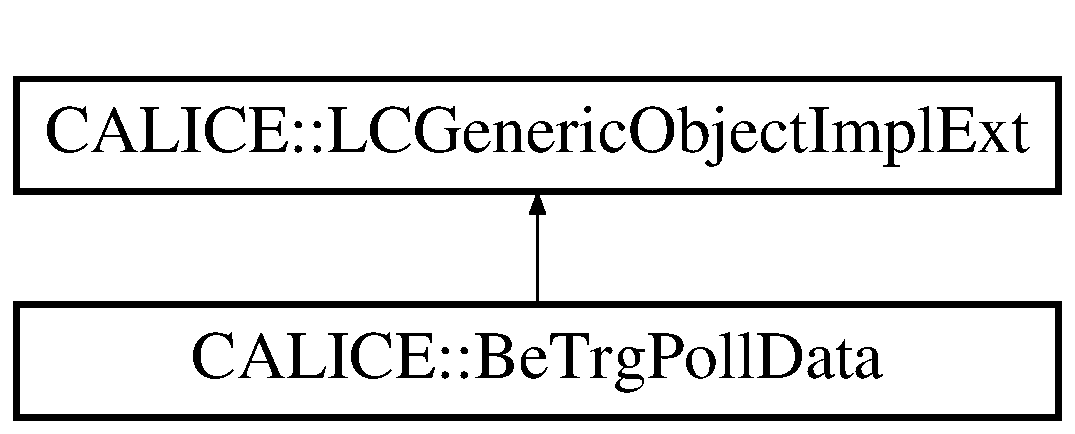
\includegraphics[height=2cm]{classCALICE_1_1BeTrgPollData}
\end{center}
\end{figure}
\subsection*{Public Member Functions}
\begin{DoxyCompactItemize}
\item 
{\bf BeTrgPollData} ()\label{classCALICE_1_1BeTrgPollData_a057354fffb3480442ed0c56bd161d84a}

\begin{DoxyCompactList}\small\item\em Default Constructor. \item\end{DoxyCompactList}\item 
{\bf BeTrgPollData} (LCObject $\ast$obj)\label{classCALICE_1_1BeTrgPollData_a058b62681a118d4cc5ffce52916cbcc5}

\begin{DoxyCompactList}\small\item\em A copy constructor. \item\end{DoxyCompactList}\item 
virtual {\bf $\sim$BeTrgPollData} ()\label{classCALICE_1_1BeTrgPollData_a5c9f105b897e0636f88eeb449694c11d}

\begin{DoxyCompactList}\small\item\em The destructor. \item\end{DoxyCompactList}\item 
{\bf BeTrgPollData} \& {\bf setBoardID} (int boardID)
\begin{DoxyCompactList}\small\item\em set the packed board id. \item\end{DoxyCompactList}\item 
int {\bf getBoardID} () const \label{classCALICE_1_1BeTrgPollData_a5141403dac81c51d98f1f84633756c7d}

\begin{DoxyCompactList}\small\item\em get the board id \item\end{DoxyCompactList}\item 
{\bf BeTrgPollData} \& {\bf setRecordLabel} (int label)\label{classCALICE_1_1BeTrgPollData_a7ff5667fae7e50368b2d56fa395bcfcc}

\begin{DoxyCompactList}\small\item\em Set the Record Label. \item\end{DoxyCompactList}\item 
short {\bf getRecordLabel} () const \label{classCALICE_1_1BeTrgPollData_aa28da3731e1d2ee372d3bdab3595610f}

\begin{DoxyCompactList}\small\item\em Return the Record Label. \item\end{DoxyCompactList}\item 
{\bf BeTrgPollData} \& {\bf setStartTime} (struct tm $\ast$startTime, int startTimemus)\label{classCALICE_1_1BeTrgPollData_a9a72f0707c23960f0ff1bc815590e327}

\begin{DoxyCompactList}\small\item\em set the start time We store Year, Month, Day and Hour, Minute, Second and microsceconds seperately We store UTC!!!! \item\end{DoxyCompactList}\item 
LCTime {\bf getStartTime} ()\label{classCALICE_1_1BeTrgPollData_ab10dba32878399a29531258a4b9c861c}

\begin{DoxyCompactList}\small\item\em returns the start time \item\end{DoxyCompactList}\item 
{\bf BeTrgPollData} \& {\bf setEndTime} (struct tm $\ast$endTime, int endTimemus)\label{classCALICE_1_1BeTrgPollData_a20bde7a4d727cb651db1060c8950b262}

\begin{DoxyCompactList}\small\item\em set the end time (see set of start time) \item\end{DoxyCompactList}\item 
LCTime {\bf getEndTime} ()\label{classCALICE_1_1BeTrgPollData_a6b6279c993919741cbd248cc1e13b4d1}

\begin{DoxyCompactList}\small\item\em returns the end time (see start time) \item\end{DoxyCompactList}\item 
{\bf BeTrgPollData} \& {\bf setMaximumTime} (int maxTimesec, int maxTimemus)\label{classCALICE_1_1BeTrgPollData_ad5db0ea39364cb7ffc2c49402ea9e01e}

\begin{DoxyCompactList}\small\item\em set the maximum time \item\end{DoxyCompactList}\item 
int {\bf getMaximumTimeSec} ()
\begin{DoxyCompactList}\small\item\em returns the maximum time sec. \item\end{DoxyCompactList}\item 
int {\bf getMaximumTimeMus} ()
\begin{DoxyCompactList}\small\item\em returns the maximum time musec. \item\end{DoxyCompactList}\item 
{\bf BeTrgPollData} \& {\bf setNumberOfPolls} (int numPolls)\label{classCALICE_1_1BeTrgPollData_a8914ec67d71bd59f42001db6ace1bcf2}

\begin{DoxyCompactList}\small\item\em set the number of polls \item\end{DoxyCompactList}\item 
int {\bf getNumberOfPolls} ()\label{classCALICE_1_1BeTrgPollData_adb334ced5c76c3e78d3375997795f510}

\begin{DoxyCompactList}\small\item\em returns the number of polls time \item\end{DoxyCompactList}\item 
{\bf BeTrgPollData} \& {\bf setTimeout} (int timeout)\label{classCALICE_1_1BeTrgPollData_a74ff7471b2da9bb422f0ef380dc6d2b0}

\begin{DoxyCompactList}\small\item\em set the info on timeout \item\end{DoxyCompactList}\item 
bool {\bf isTimeout} ()\label{classCALICE_1_1BeTrgPollData_af4dc72493caeee97b9ae3353bb7e6617}

\begin{DoxyCompactList}\small\item\em timeout set? \item\end{DoxyCompactList}\item 
const std::string {\bf getTypeName} () const \label{classCALICE_1_1BeTrgPollData_a46de676202c64beca2a9ae254a6e3486}

\begin{DoxyCompactList}\small\item\em returns the the type name \item\end{DoxyCompactList}\item 
const std::string {\bf getDataDescription} () const \label{classCALICE_1_1BeTrgPollData_a2d5728298c8256ec4daaa034b1bb2106}

\begin{DoxyCompactList}\small\item\em returns a brief description of the data stored \item\end{DoxyCompactList}\item 
std::ostream \& {\bf print} (std::ostream \&ostrm)\label{classCALICE_1_1BeTrgPollData_a528e115723725ae3366fe07ec73efeb6}

\begin{DoxyCompactList}\small\item\em dumps data content \item\end{DoxyCompactList}\end{DoxyCompactItemize}


\subsection{Detailed Description}
Class to store info on trigger polling, This is useful to detect a softtrigger among e.g. beam trigger if e.g. the beam has disappeared \begin{DoxyAuthor}{Author}
R. P�schl (LAL Orsay) 
\end{DoxyAuthor}
\begin{DoxyDate}{Date}
Jul 02 2006 
\end{DoxyDate}


Definition at line 39 of file BeTrgPollData.hh.

\subsection{Member Function Documentation}
\index{CALICE::BeTrgPollData@{CALICE::BeTrgPollData}!getMaximumTimeMus@{getMaximumTimeMus}}
\index{getMaximumTimeMus@{getMaximumTimeMus}!CALICE::BeTrgPollData@{CALICE::BeTrgPollData}}
\subsubsection[{getMaximumTimeMus}]{\setlength{\rightskip}{0pt plus 5cm}int CALICE::BeTrgPollData::getMaximumTimeMus ()\hspace{0.3cm}{\ttfamily  [inline]}}\label{classCALICE_1_1BeTrgPollData_ace45885ebc9a2eaec02494b0bb0a5eda}


returns the maximum time musec. part 

Definition at line 226 of file BeTrgPollData.hh.

References CALICE::LCGenericObjectImplExt::obj().

Referenced by print().\index{CALICE::BeTrgPollData@{CALICE::BeTrgPollData}!getMaximumTimeSec@{getMaximumTimeSec}}
\index{getMaximumTimeSec@{getMaximumTimeSec}!CALICE::BeTrgPollData@{CALICE::BeTrgPollData}}
\subsubsection[{getMaximumTimeSec}]{\setlength{\rightskip}{0pt plus 5cm}int CALICE::BeTrgPollData::getMaximumTimeSec ()\hspace{0.3cm}{\ttfamily  [inline]}}\label{classCALICE_1_1BeTrgPollData_a6df7064ded7d9b57acece6987b770ec4}


returns the maximum time sec. part 

Definition at line 217 of file BeTrgPollData.hh.

References CALICE::LCGenericObjectImplExt::obj().

Referenced by print().\index{CALICE::BeTrgPollData@{CALICE::BeTrgPollData}!setBoardID@{setBoardID}}
\index{setBoardID@{setBoardID}!CALICE::BeTrgPollData@{CALICE::BeTrgPollData}}
\subsubsection[{setBoardID}]{\setlength{\rightskip}{0pt plus 5cm}{\bf BeTrgPollData}\& CALICE::BeTrgPollData::setBoardID (int {\em boardID})\hspace{0.3cm}{\ttfamily  [inline]}}\label{classCALICE_1_1BeTrgPollData_a621ba825e9be0fbaf2258870a4a206a7}


set the packed board id. \begin{DoxySeeAlso}{See also}
\doxyref{BoardID}{p.}{classCALICE_1_1BoardID} 
\end{DoxySeeAlso}


Definition at line 79 of file BeTrgPollData.hh.

References CALICE::LCGenericObjectImplExt::obj().

The documentation for this class was generated from the following file:\begin{DoxyCompactItemize}
\item 
BeTrgPollData.hh\end{DoxyCompactItemize}

\section{CALICE::BinnedVector$<$ K, D $>$ Class Template Reference}
\label{classCALICE_1_1BinnedVector}\index{CALICE::BinnedVector@{CALICE::BinnedVector}}


Template class to store data via a linear binned keys.  


{\ttfamily \#include $<$BinnedVector.hh$>$}\subsection*{Public Member Functions}
\begin{DoxyCompactItemize}
\item 
{\bf BinnedVector} ()
\begin{DoxyCompactList}\small\item\em standard constructor \item\end{DoxyCompactList}\item 
{\bf BinnedVector} (const unsigned int N, const K \&minRange, const K \&maxRange, const D \&initValue)
\begin{DoxyCompactList}\small\item\em constructor which sets dimensions \item\end{DoxyCompactList}\item 
void {\bf setBinning} (const unsigned int N, const K \&minRange, const K \&maxRange, const D \&initValue)
\begin{DoxyCompactList}\small\item\em function to set the dimensions \item\end{DoxyCompactList}\item 
D \& {\bf operator[$\,$]} (const K \&position)
\begin{DoxyCompactList}\small\item\em access operator \item\end{DoxyCompactList}\item 
const D \& {\bf operator[$\,$]} (const K \&position) const 
\begin{DoxyCompactList}\small\item\em const access operator \item\end{DoxyCompactList}\item 
void {\bf clear} ()
\begin{DoxyCompactList}\small\item\em clear content of bins \item\end{DoxyCompactList}\item 
const std::vector$<$ D $>$ \& {\bf getVector} () const 
\begin{DoxyCompactList}\small\item\em get vector of bins \item\end{DoxyCompactList}\item 
std::vector$<$ K $>$ {\bf getBinCenters} () const 
\begin{DoxyCompactList}\small\item\em get vector of bin centers \item\end{DoxyCompactList}\end{DoxyCompactItemize}
\subsection*{Private Member Functions}
\begin{DoxyCompactItemize}
\item 
unsigned int {\bfseries getIndex} (const K \&position) const \label{classCALICE_1_1BinnedVector_a4123e06e0d7a11932c077dc5fe493f1a}

\end{DoxyCompactItemize}
\subsection*{Private Attributes}
\begin{DoxyCompactItemize}
\item 
K {\bfseries \_\-binWidth}\label{classCALICE_1_1BinnedVector_afeaf367990f430e62c61ab0683783fd1}

\item 
K {\bfseries \_\-minRange}\label{classCALICE_1_1BinnedVector_af613299eaafb750fde3806ee35888911}

\item 
K {\bfseries \_\-maxRange}\label{classCALICE_1_1BinnedVector_a91b5b2679ffa43db2731fe9fff33c108}

\item 
unsigned int {\bfseries \_\-N}\label{classCALICE_1_1BinnedVector_ab6da09732d112c6d308208eb634f8fdd}

\item 
std::vector$<$ D $>$ {\bfseries \_\-data}\label{classCALICE_1_1BinnedVector_a774e0934eb7e9115ceff381367cdb251}

\item 
D {\bfseries \_\-default}\label{classCALICE_1_1BinnedVector_ac882272e3b94ce45830b5f44f8c0309d}

\end{DoxyCompactItemize}


\subsection{Detailed Description}
\subsubsection*{template$<$class K, class D$>$ class CALICE::BinnedVector$<$ K, D $>$}

Template class to store data via a linear binned keys. This is like a histogram, but without graphical functionallity.


\begin{DoxyParams}{Parameters}
\item[{\em K}]type of the key \item[{\em D}]type of the data\end{DoxyParams}
\begin{DoxyAuthor}{Author}
{\tt Benjamin.Lutz@desy.de} 
\end{DoxyAuthor}
\begin{DoxyVersion}{Version}
0.2 
\end{DoxyVersion}
\begin{DoxyDate}{Date}
October 2009 
\end{DoxyDate}


Definition at line 24 of file BinnedVector.hh.

\subsection{Constructor \& Destructor Documentation}
\index{CALICE::BinnedVector@{CALICE::BinnedVector}!BinnedVector@{BinnedVector}}
\index{BinnedVector@{BinnedVector}!CALICE::BinnedVector@{CALICE::BinnedVector}}
\subsubsection[{BinnedVector}]{\setlength{\rightskip}{0pt plus 5cm}template$<$class K , class D $>$ {\bf CALICE::BinnedVector}$<$ K, D $>$::{\bf BinnedVector} ()\hspace{0.3cm}{\ttfamily  [inline]}}\label{classCALICE_1_1BinnedVector_ac4a4d7f849e54dd2ca206c6c4c3b9a4d}


standard constructor \begin{DoxyWarning}{Warning}
Dimensions have to be set with \doxyref{setBinning()}{p.}{classCALICE_1_1BinnedVector_a0a556d0e061a26a4a9f36c68bdaa5605} before the vector can be used. 
\end{DoxyWarning}


Definition at line 103 of file BinnedVector.hh.\index{CALICE::BinnedVector@{CALICE::BinnedVector}!BinnedVector@{BinnedVector}}
\index{BinnedVector@{BinnedVector}!CALICE::BinnedVector@{CALICE::BinnedVector}}
\subsubsection[{BinnedVector}]{\setlength{\rightskip}{0pt plus 5cm}template$<$class K, class D$>$ {\bf CALICE::BinnedVector}$<$ K, D $>$::{\bf BinnedVector} (const unsigned int {\em N}, \/  const K \& {\em minRange}, \/  const K \& {\em maxRange}, \/  const D \& {\em initValue})\hspace{0.3cm}{\ttfamily  [inline]}}\label{classCALICE_1_1BinnedVector_ac82537603208f443464a68274d1b0003}


constructor which sets dimensions 
\begin{DoxyParams}{Parameters}
\item[{\em N}]number bins (without under and over range bins) \item[{\em minRange}]lower end of range \item[{\em maxRange}]upper end of range \item[{\em initValue}]value for initialisation of bins \end{DoxyParams}


Definition at line 107 of file BinnedVector.hh.

References CALICE::BinnedVector$<$ K, D $>$::setBinning().

\subsection{Member Function Documentation}
\index{CALICE::BinnedVector@{CALICE::BinnedVector}!clear@{clear}}
\index{clear@{clear}!CALICE::BinnedVector@{CALICE::BinnedVector}}
\subsubsection[{clear}]{\setlength{\rightskip}{0pt plus 5cm}template$<$class K , class D $>$ void {\bf CALICE::BinnedVector}$<$ K, D $>$::clear ()\hspace{0.3cm}{\ttfamily  [inline]}}\label{classCALICE_1_1BinnedVector_aabcdd48468006c8518ae4a5623aa21ab}


clear content of bins all bins will be set to initValue 

Definition at line 112 of file BinnedVector.hh.

Referenced by CALICE::BinnedVector$<$ K, D $>$::setBinning().\index{CALICE::BinnedVector@{CALICE::BinnedVector}!getBinCenters@{getBinCenters}}
\index{getBinCenters@{getBinCenters}!CALICE::BinnedVector@{CALICE::BinnedVector}}
\subsubsection[{getBinCenters}]{\setlength{\rightskip}{0pt plus 5cm}template$<$class K , class D $>$ std::vector$<$ K $>$ {\bf CALICE::BinnedVector}$<$ K, D $>$::getBinCenters () const\hspace{0.3cm}{\ttfamily  [inline]}}\label{classCALICE_1_1BinnedVector_abab5c9e035268638c18327f8a3826d43}


get vector of bin centers the vector starts with the under range bin and ends with the over range bin

\begin{DoxyReturn}{Returns}
vector of bin centers 
\end{DoxyReturn}


Definition at line 158 of file BinnedVector.hh.\index{CALICE::BinnedVector@{CALICE::BinnedVector}!getVector@{getVector}}
\index{getVector@{getVector}!CALICE::BinnedVector@{CALICE::BinnedVector}}
\subsubsection[{getVector}]{\setlength{\rightskip}{0pt plus 5cm}template$<$class K, class D$>$ const std::vector$<$D$>$\& {\bf CALICE::BinnedVector}$<$ K, D $>$::getVector () const\hspace{0.3cm}{\ttfamily  [inline]}}\label{classCALICE_1_1BinnedVector_ab7bfb5aefe1cdb0e89664f30d15e48e3}


get vector of bins the vector starts with the under range bin and ends with the over range bin

\begin{DoxyReturn}{Returns}
vector of bins 
\end{DoxyReturn}


Definition at line 78 of file BinnedVector.hh.

Referenced by CALICE::TcmtEventIdentifier::addResults(), and CALICE::TcmtEventIdentifier::process().\index{CALICE::BinnedVector@{CALICE::BinnedVector}!operator[]@{operator[]}}
\index{operator[]@{operator[]}!CALICE::BinnedVector@{CALICE::BinnedVector}}
\subsubsection[{operator[]}]{\setlength{\rightskip}{0pt plus 5cm}template$<$class K, class D $>$ const D \& {\bf CALICE::BinnedVector}$<$ K, D $>$::operator[$\,$] (const K \& {\em position}) const\hspace{0.3cm}{\ttfamily  [inline]}}\label{classCALICE_1_1BinnedVector_aac7fe817f2b702c34a9eff4fd3b205bb}


const access operator 
\begin{DoxyParams}{Parameters}
\item[{\em position}]key to find bin \end{DoxyParams}
\begin{DoxyReturn}{Returns}
value at key 
\end{DoxyReturn}


Definition at line 153 of file BinnedVector.hh.\index{CALICE::BinnedVector@{CALICE::BinnedVector}!operator[]@{operator[]}}
\index{operator[]@{operator[]}!CALICE::BinnedVector@{CALICE::BinnedVector}}
\subsubsection[{operator[]}]{\setlength{\rightskip}{0pt plus 5cm}template$<$class K, class D $>$ D \& {\bf CALICE::BinnedVector}$<$ K, D $>$::operator[$\,$] (const K \& {\em position})\hspace{0.3cm}{\ttfamily  [inline]}}\label{classCALICE_1_1BinnedVector_a6b32d7391a66dd275f51c92db106f0e7}


access operator 
\begin{DoxyParams}{Parameters}
\item[{\em position}]key to find bin \end{DoxyParams}
\begin{DoxyReturn}{Returns}
value at key 
\end{DoxyReturn}


Definition at line 148 of file BinnedVector.hh.\index{CALICE::BinnedVector@{CALICE::BinnedVector}!setBinning@{setBinning}}
\index{setBinning@{setBinning}!CALICE::BinnedVector@{CALICE::BinnedVector}}
\subsubsection[{setBinning}]{\setlength{\rightskip}{0pt plus 5cm}template$<$class K, class D$>$ void {\bf CALICE::BinnedVector}$<$ K, D $>$::setBinning (const unsigned int {\em N}, \/  const K \& {\em minRange}, \/  const K \& {\em maxRange}, \/  const D \& {\em initValue})\hspace{0.3cm}{\ttfamily  [inline]}}\label{classCALICE_1_1BinnedVector_a0a556d0e061a26a4a9f36c68bdaa5605}


function to set the dimensions 
\begin{DoxyParams}{Parameters}
\item[{\em N}]number bins (without under and over range bins) \item[{\em minRange}]lower end of range \item[{\em maxRange}]upper end of range \item[{\em initValue}]value for initialisation of bins \end{DoxyParams}


Definition at line 120 of file BinnedVector.hh.

References CALICE::BinnedVector$<$ K, D $>$::clear().

Referenced by CALICE::BinnedVector$<$ K, D $>$::BinnedVector(), and CALICE::TcmtEventIdentifier::TcmtEventIdentifier().

The documentation for this class was generated from the following file:\begin{DoxyCompactItemize}
\item 
BinnedVector.hh\end{DoxyCompactItemize}

\section{CALICE::BitSet Class Reference}
\label{classCALICE_1_1BitSet}\index{CALICE::BitSet@{CALICE::BitSet}}


Base class for easy definition of bit sets.  


{\ttfamily \#include $<$BitSet.hh$>$}Inheritance diagram for CALICE::BitSet::\begin{figure}[H]
\begin{center}
\leavevmode
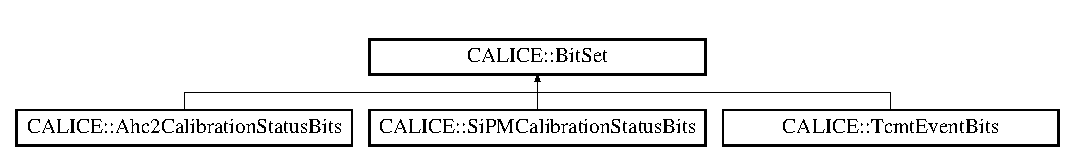
\includegraphics[height=1.72839cm]{classCALICE_1_1BitSet}
\end{center}
\end{figure}
\subsection*{Public Member Functions}
\begin{DoxyCompactItemize}
\item 
int {\bf getInt} () const 
\begin{DoxyCompactList}\small\item\em get integer corresponding to the bits \item\end{DoxyCompactList}\item 
void {\bf setBits} (const int value)
\begin{DoxyCompactList}\small\item\em set all bits with an integer \item\end{DoxyCompactList}\item 
std::vector$<$ int $>$ {\bf getIntVec} () const 
\begin{DoxyCompactList}\small\item\em get vector of ints with elements corresponding to the single bits (1 for true and 0 for false) \item\end{DoxyCompactList}\item 
void {\bf clear} ()\label{classCALICE_1_1BitSet_abd6be6d671e597c9c04afd73d25f7b6a}

\begin{DoxyCompactList}\small\item\em clear all bits to 0 \item\end{DoxyCompactList}\end{DoxyCompactItemize}
\subsection*{Protected Member Functions}
\begin{DoxyCompactItemize}
\item 
{\bf BitSet} (const unsigned int maxBits, const int value=0x0)
\begin{DoxyCompactList}\small\item\em constructur \item\end{DoxyCompactList}\item 
bool {\bf getBit} (unsigned int bitNo) const 
\begin{DoxyCompactList}\small\item\em get function for bit number \item\end{DoxyCompactList}\item 
void {\bf setBit} (unsigned int bitNo, bool state)
\begin{DoxyCompactList}\small\item\em set function for bit number \item\end{DoxyCompactList}\end{DoxyCompactItemize}
\subsection*{Private Attributes}
\begin{DoxyCompactItemize}
\item 
int {\bfseries \_\-bits}\label{classCALICE_1_1BitSet_acb489ad5309a1343dc9d368fbfabb4e7}

\item 
unsigned int {\bfseries \_\-maxBits}\label{classCALICE_1_1BitSet_a0105ecaa0c1f03c666f90f3d3b7207c6}

\end{DoxyCompactItemize}


\subsection{Detailed Description}
Base class for easy definition of bit sets. Derived classes have to define the meaning of the bits. No instantiation possible.

\begin{DoxyAuthor}{Author}
{\tt Benjamin.Lutz@desy.de} 
\end{DoxyAuthor}
\begin{DoxyDate}{Date}
November 2009 
\end{DoxyDate}
\begin{DoxyVersion}{Version}
1.0 
\end{DoxyVersion}


Definition at line 18 of file BitSet.hh.

\subsection{Constructor \& Destructor Documentation}
\index{CALICE::BitSet@{CALICE::BitSet}!BitSet@{BitSet}}
\index{BitSet@{BitSet}!CALICE::BitSet@{CALICE::BitSet}}
\subsubsection[{BitSet}]{\setlength{\rightskip}{0pt plus 5cm}CALICE::BitSet::BitSet (const unsigned int {\em maxBits}, \/  const int {\em value} = {\ttfamily 0x0})\hspace{0.3cm}{\ttfamily  [inline, protected]}}\label{classCALICE_1_1BitSet_a73f400c579b2731fc366faf7fa873aa9}


constructur maximum number of bits defines the size of the returned vector


\begin{DoxyParams}{Parameters}
\item[\mbox{$\leftarrow$} {\em maxBits}]maximum number of bits \item[\mbox{$\leftarrow$} {\em value}]to initialise to different than 0 \end{DoxyParams}


Definition at line 69 of file BitSet.hh.

\subsection{Member Function Documentation}
\index{CALICE::BitSet@{CALICE::BitSet}!getBit@{getBit}}
\index{getBit@{getBit}!CALICE::BitSet@{CALICE::BitSet}}
\subsubsection[{getBit}]{\setlength{\rightskip}{0pt plus 5cm}bool CALICE::BitSet::getBit (unsigned int {\em bitNo}) const\hspace{0.3cm}{\ttfamily  [inline, protected]}}\label{classCALICE_1_1BitSet_a0ffe3a5bdb4f4f5ec069c4330fef672b}


get function for bit number 
\begin{DoxyParams}{Parameters}
\item[{\em bitNo}]number of the bit to return \end{DoxyParams}
\begin{DoxyReturn}{Returns}
state of bit 
\end{DoxyReturn}


Definition at line 80 of file BitSet.hh.

Referenced by getIntVec(), CALICE::TcmtEventBits::hasMaxNumberHitsMuon(), CALICE::TcmtEventBits::hasMaxNumberMuonLikeTowers(), CALICE::TcmtEventBits::hasMaxSumEnergyMuon(), CALICE::TcmtEventBits::hasMinNumberHitsMuon(), CALICE::TcmtEventBits::hasMinNumberMuonLikeLayers(), CALICE::TcmtEventBits::hasMinNumberMuonLikeTowers(), CALICE::TcmtEventBits::hasMinSumEnergyMuon(), CALICE::TcmtEventBits::isLeakage(), CALICE::TcmtEventBits::isMuon(), and CALICE::TcmtEventBits::isPedestal().\index{CALICE::BitSet@{CALICE::BitSet}!getInt@{getInt}}
\index{getInt@{getInt}!CALICE::BitSet@{CALICE::BitSet}}
\subsubsection[{getInt}]{\setlength{\rightskip}{0pt plus 5cm}int CALICE::BitSet::getInt () const\hspace{0.3cm}{\ttfamily  [inline]}}\label{classCALICE_1_1BitSet_a148efced5e1ce099391216e2f4c9718a}


get integer corresponding to the bits \begin{DoxyReturn}{Returns}
integer with the bits set 
\end{DoxyReturn}


Definition at line 27 of file BitSet.hh.

Referenced by CALICE::TcmtEventIdentifier::addResults().\index{CALICE::BitSet@{CALICE::BitSet}!getIntVec@{getIntVec}}
\index{getIntVec@{getIntVec}!CALICE::BitSet@{CALICE::BitSet}}
\subsubsection[{getIntVec}]{\setlength{\rightskip}{0pt plus 5cm}std::vector$<$int$>$ CALICE::BitSet::getIntVec () const\hspace{0.3cm}{\ttfamily  [inline]}}\label{classCALICE_1_1BitSet_a807161095aee85a74b6f520f32690ace}


get vector of ints with elements corresponding to the single bits (1 for true and 0 for false) \begin{DoxyReturn}{Returns}
vector of integers of single bits 
\end{DoxyReturn}


Definition at line 44 of file BitSet.hh.

References getBit().

Referenced by CALICE::TcmtEventIdentifier::addResults().\index{CALICE::BitSet@{CALICE::BitSet}!setBit@{setBit}}
\index{setBit@{setBit}!CALICE::BitSet@{CALICE::BitSet}}
\subsubsection[{setBit}]{\setlength{\rightskip}{0pt plus 5cm}void CALICE::BitSet::setBit (unsigned int {\em bitNo}, \/  bool {\em state})\hspace{0.3cm}{\ttfamily  [inline, protected]}}\label{classCALICE_1_1BitSet_ae1b313a2e4a97fd9f197239f4abb9a49}


set function for bit number 
\begin{DoxyParams}{Parameters}
\item[{\em bitNo}]number of the bit to set \item[{\em state}]state to witch the bit gets set \end{DoxyParams}


Definition at line 87 of file BitSet.hh.\index{CALICE::BitSet@{CALICE::BitSet}!setBits@{setBits}}
\index{setBits@{setBits}!CALICE::BitSet@{CALICE::BitSet}}
\subsubsection[{setBits}]{\setlength{\rightskip}{0pt plus 5cm}void CALICE::BitSet::setBits (const int {\em value})\hspace{0.3cm}{\ttfamily  [inline]}}\label{classCALICE_1_1BitSet_a17ed04fb84b1be0b476312d046333704}


set all bits with an integer 
\begin{DoxyParams}{Parameters}
\item[\mbox{$\leftarrow$} {\em value}]integer with the bits \end{DoxyParams}


Definition at line 34 of file BitSet.hh.

The documentation for this class was generated from the following file:\begin{DoxyCompactItemize}
\item 
BitSet.hh\end{DoxyCompactItemize}

\section{CALICE::BmlCaen1290ConfigurationBlock Class Reference}
\label{classCALICE_1_1BmlCaen1290ConfigurationBlock}\index{CALICE::BmlCaen1290ConfigurationBlock@{CALICE::BmlCaen1290ConfigurationBlock}}
Inheritance diagram for CALICE::BmlCaen1290ConfigurationBlock::\begin{figure}[H]
\begin{center}
\leavevmode
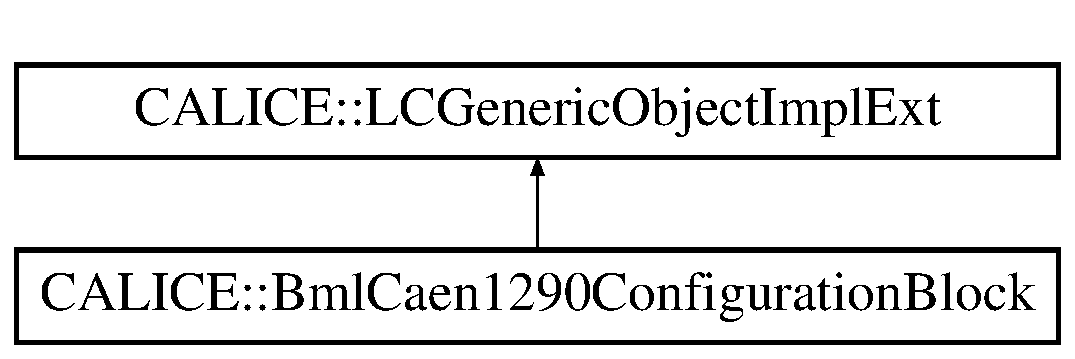
\includegraphics[height=2cm]{classCALICE_1_1BmlCaen1290ConfigurationBlock}
\end{center}
\end{figure}
\subsection*{Public Member Functions}
\begin{DoxyCompactItemize}
\item 
{\bfseries BmlCaen1290ConfigurationBlock} (LCObject $\ast$obj)\label{classCALICE_1_1BmlCaen1290ConfigurationBlock_a2d4ea6c8b939a48a1236a7d38087a469}

\item 
{\bf BmlCaen1290ConfigurationBlock} \& {\bfseries setBoardID} (int boardid)\label{classCALICE_1_1BmlCaen1290ConfigurationBlock_a26eb94a1bcb0960c8c36a8183e88fb7b}

\item 
int {\bfseries getBoardID} ()\label{classCALICE_1_1BmlCaen1290ConfigurationBlock_a7388b9a32d541f9f810e618e4e0090a6}

\item 
{\bf BmlCaen1290ConfigurationBlock} \& {\bfseries setBaseAddress} (int baseaddress)\label{classCALICE_1_1BmlCaen1290ConfigurationBlock_a91ac6d8a2c5ed25692fd031b032286d8}

\item 
short {\bfseries getBaseAddress} () const \label{classCALICE_1_1BmlCaen1290ConfigurationBlock_aa3350ed9c44286ce22dadefa15a3f2b9}

\item 
{\bf BmlCaen1290ConfigurationBlock} \& {\bfseries setRecordLabel} (int label)\label{classCALICE_1_1BmlCaen1290ConfigurationBlock_aa352775bfd0fefd8f159007a848680c7}

\item 
short {\bfseries getRecordLabel} () const \label{classCALICE_1_1BmlCaen1290ConfigurationBlock_aba8ba99a96410f121cbfe9ae0a0712c6}

\item 
{\bf BmlCaen1290ConfigurationBlock} \& {\bfseries setControlRegister} (int controlregister)\label{classCALICE_1_1BmlCaen1290ConfigurationBlock_aac6dd9b7a93bbe7018580d7ed2541994}

\item 
int {\bfseries getControlRegister} ()\label{classCALICE_1_1BmlCaen1290ConfigurationBlock_a44e50c75db94105d7a558450b99b2d5a}

\item 
{\bf BmlCaen1290ConfigurationBlock} \& {\bfseries setInterruptRegister} (int interruptregister)\label{classCALICE_1_1BmlCaen1290ConfigurationBlock_a81599fbfb68917487f0c62b74022fd11}

\item 
int {\bfseries getInterruptRegister} ()\label{classCALICE_1_1BmlCaen1290ConfigurationBlock_aaee03cf540e2494f17dc7837f32137d0}

\item 
{\bf BmlCaen1290ConfigurationBlock} \& {\bfseries setCountRegister} (int countregister)\label{classCALICE_1_1BmlCaen1290ConfigurationBlock_a457aedeb41da454148865f66f82c1ba4}

\item 
int {\bfseries getCountRegister} ()\label{classCALICE_1_1BmlCaen1290ConfigurationBlock_a0c3d644ba875e29f3ce31fb0da51941f}

\item 
void {\bfseries print} (std::ostream \&os)\label{classCALICE_1_1BmlCaen1290ConfigurationBlock_adbb29adf8d9fd7ecd6e7176ac4348e13}

\item 
const std::string {\bfseries getTypeName} () const \label{classCALICE_1_1BmlCaen1290ConfigurationBlock_a1c568fad015045482af859b6432b1838}

\item 
const std::string {\bfseries getDataDescription} () const \label{classCALICE_1_1BmlCaen1290ConfigurationBlock_a20a49557bcb139b1047748ce0cbd809a}

\end{DoxyCompactItemize}


\subsection{Detailed Description}


Definition at line 22 of file BmlCaen1290ConfigurationBlock.hh.

The documentation for this class was generated from the following file:\begin{DoxyCompactItemize}
\item 
BmlCaen1290ConfigurationBlock.hh\end{DoxyCompactItemize}

\section{CALICE::BmlCaen767ConfigurationBlock Class Reference}
\label{classCALICE_1_1BmlCaen767ConfigurationBlock}\index{CALICE::BmlCaen767ConfigurationBlock@{CALICE::BmlCaen767ConfigurationBlock}}


Class to store configuration data of the 767 Caen TDC obsolete as of 31/10/10, replaced by \doxyref{BmlCaenConfigurationBlock}{p.}{classCALICE_1_1BmlCaenConfigurationBlock}, kept for backward compatibility of the code.  


{\ttfamily \#include $<$BmlCaen767ConfigurationBlock.hh$>$}Inheritance diagram for CALICE::BmlCaen767ConfigurationBlock::\begin{figure}[H]
\begin{center}
\leavevmode
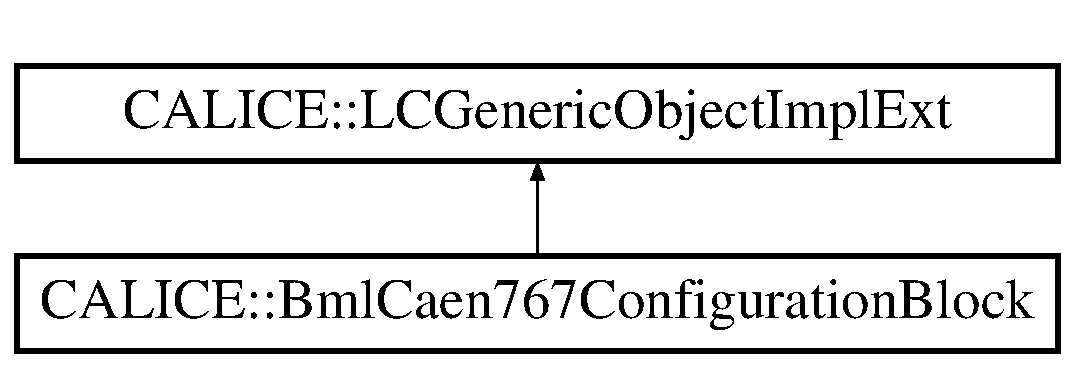
\includegraphics[height=2cm]{classCALICE_1_1BmlCaen767ConfigurationBlock}
\end{center}
\end{figure}
\subsection*{Public Member Functions}
\begin{DoxyCompactItemize}
\item 
{\bfseries BmlCaen767ConfigurationBlock} (LCObject $\ast$obj)\label{classCALICE_1_1BmlCaen767ConfigurationBlock_a9d74204e08b6b2b3f8af2e33594bc427}

\item 
{\bf BmlCaen767ConfigurationBlock} \& {\bfseries setBoardID} (int boardid)\label{classCALICE_1_1BmlCaen767ConfigurationBlock_a45d5e9f1b6b625e98498fe44e4e84b99}

\item 
int {\bfseries getBoardID} ()\label{classCALICE_1_1BmlCaen767ConfigurationBlock_aa5ed1065d3621938708124ad46ed42cd}

\item 
{\bf BmlCaen767ConfigurationBlock} \& {\bfseries setBaseAddress} (int baseaddress)\label{classCALICE_1_1BmlCaen767ConfigurationBlock_af82dcd49f43b478d53d1817a84b72172}

\item 
short {\bfseries getBaseAddress} () const \label{classCALICE_1_1BmlCaen767ConfigurationBlock_a0afa51af661dd59e966b3d9853bd5815}

\item 
{\bf BmlCaen767ConfigurationBlock} \& {\bfseries setRecordLabel} (int label)\label{classCALICE_1_1BmlCaen767ConfigurationBlock_a3c823c83fcfcc31b97c6841623144fa7}

\item 
short {\bfseries getRecordLabel} () const \label{classCALICE_1_1BmlCaen767ConfigurationBlock_a1e217f2e31b14e11233816c28a5a31e8}

\item 
{\bf BmlCaen767ConfigurationBlock} \& {\bfseries setControlRegister} (int controlregister)\label{classCALICE_1_1BmlCaen767ConfigurationBlock_aa04af84d56b57a3fbbd773b634515ba8}

\item 
int {\bfseries getControlRegister} ()\label{classCALICE_1_1BmlCaen767ConfigurationBlock_a4ca9caf9f38105f5ae42ebb26e14949d}

\item 
{\bf BmlCaen767ConfigurationBlock} \& {\bfseries setInterruptRegister} (int interruptregister)\label{classCALICE_1_1BmlCaen767ConfigurationBlock_ac915c9120ba54f8a499a09ba97b55c70}

\item 
int {\bfseries getInterruptRegister} ()\label{classCALICE_1_1BmlCaen767ConfigurationBlock_a24a4cc23e5d53f80a349c6fc75609e13}

\item 
void {\bfseries print} (std::ostream \&os)\label{classCALICE_1_1BmlCaen767ConfigurationBlock_a0187bcd935e12e88d5fadbae84fdb224}

\item 
const std::string {\bfseries getTypeName} () const \label{classCALICE_1_1BmlCaen767ConfigurationBlock_aeb8004b87f36dda36e7c713f38e618b5}

\item 
const std::string {\bfseries getDataDescription} () const \label{classCALICE_1_1BmlCaen767ConfigurationBlock_aea6f25e18e5758e6c82df338b13d05a1}

\end{DoxyCompactItemize}


\subsection{Detailed Description}
Class to store configuration data of the 767 Caen TDC obsolete as of 31/10/10, replaced by \doxyref{BmlCaenConfigurationBlock}{p.}{classCALICE_1_1BmlCaenConfigurationBlock}, kept for backward compatibility of the code. \begin{DoxyAuthor}{Author}
R.Poeschl (LAL Orsay) 
\end{DoxyAuthor}
\begin{DoxyDate}{Date}
Aug 01 2006 
\end{DoxyDate}


Definition at line 30 of file BmlCaen767ConfigurationBlock.hh.

The documentation for this class was generated from the following file:\begin{DoxyCompactItemize}
\item 
BmlCaen767ConfigurationBlock.hh\end{DoxyCompactItemize}

\section{CALICE::BmlCaen767ReadoutConfigurationBlock Class Reference}
\label{classCALICE_1_1BmlCaen767ReadoutConfigurationBlock}\index{CALICE::BmlCaen767ReadoutConfigurationBlock@{CALICE::BmlCaen767ReadoutConfigurationBlock}}


Stores the configuration of the Caen767 TDC into the database At the moment I am writing this class I don't know whether they'll serve for something but it is a small uncomplicated class, so here we go.  


{\ttfamily \#include $<$BmlCaen767ReadoutConfigurationBlock.hh$>$}Inheritance diagram for CALICE::BmlCaen767ReadoutConfigurationBlock::\begin{figure}[H]
\begin{center}
\leavevmode
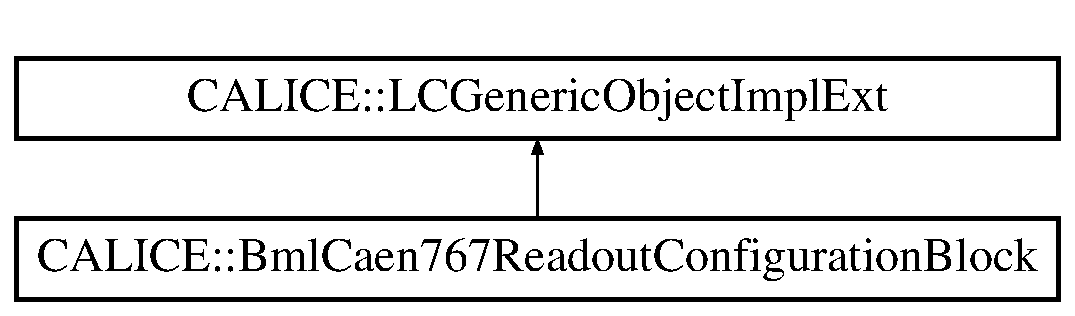
\includegraphics[height=2cm]{classCALICE_1_1BmlCaen767ReadoutConfigurationBlock}
\end{center}
\end{figure}
\subsection*{Public Member Functions}
\begin{DoxyCompactItemize}
\item 
{\bf BmlCaen767ReadoutConfigurationBlock} ()\label{classCALICE_1_1BmlCaen767ReadoutConfigurationBlock_a7b9ac595633452fbbdee1892e94773a2}

\begin{DoxyCompactList}\small\item\em Default Constructor. \item\end{DoxyCompactList}\item 
{\bf BmlCaen767ReadoutConfigurationBlock} (LCObject $\ast$obj)\label{classCALICE_1_1BmlCaen767ReadoutConfigurationBlock_aee0f6722067d06d4583bea18ffb2dc1e}

\begin{DoxyCompactList}\small\item\em 'Copy constructor' needed to interpret LCCollection read from file/database. \item\end{DoxyCompactList}\item 
{\bf BmlCaen767ReadoutConfigurationBlock} \& {\bf setCrateNumber} (int cratenumber)
\begin{DoxyCompactList}\small\item\em set the packed board id. \item\end{DoxyCompactList}\item 
int {\bf getCrateNumber} ()\label{classCALICE_1_1BmlCaen767ReadoutConfigurationBlock_a98283f15edae4729e382eaa0ef556be4}

\begin{DoxyCompactList}\small\item\em Return the crate number. \item\end{DoxyCompactList}\item 
{\bf BmlCaen767ReadoutConfigurationBlock} \& {\bf setReadPeriod} (int readperiod)\label{classCALICE_1_1BmlCaen767ReadoutConfigurationBlock_ad7910acd3e581a551f968402cb943a5d}

\begin{DoxyCompactList}\small\item\em Set the Read Period. \item\end{DoxyCompactList}\item 
unsigned int {\bf getReadPeriod} () const \label{classCALICE_1_1BmlCaen767ReadoutConfigurationBlock_a55139c919133134fc95514a97252c99b}

\begin{DoxyCompactList}\small\item\em Return the Read Period. \item\end{DoxyCompactList}\item 
{\bf BmlCaen767ReadoutConfigurationBlock} \& {\bf setBools} (bool enable, bool softtrigger, bool bltro, bool arrayro)\label{classCALICE_1_1BmlCaen767ReadoutConfigurationBlock_a0f4e57ffa62de58619397cdc8b203f42}

\begin{DoxyCompactList}\small\item\em Store the indicators of the readout mode. \item\end{DoxyCompactList}\item 
bool {\bfseries isEnabled} ()\label{classCALICE_1_1BmlCaen767ReadoutConfigurationBlock_a6a822edd1400153f4db0d779fa24862b}

\item 
bool {\bfseries isSoftTrigger} ()\label{classCALICE_1_1BmlCaen767ReadoutConfigurationBlock_ae6a1be49e52e35b4966ebc0c373bcdff}

\item 
bool {\bfseries isBltReadout} ()\label{classCALICE_1_1BmlCaen767ReadoutConfigurationBlock_a9aad9174d74e8f233e456c807f28ec97}

\item 
bool {\bfseries isArrayReadout} ()\label{classCALICE_1_1BmlCaen767ReadoutConfigurationBlock_ad67e67c908f7f4a337c9d2ea61a93229}

\item 
{\bf BmlCaen767ReadoutConfigurationBlock} \& {\bf setMode} (int mode)
\begin{DoxyCompactList}\small\item\em Store the readout mode word note that this word contains the information which you also get with the isSoftTrigger, isEnable, getCrateNumber etc. \item\end{DoxyCompactList}\item 
int {\bf getMode} ()\label{classCALICE_1_1BmlCaen767ReadoutConfigurationBlock_a317aceac7a964643ece66c7f280ed79b}

\begin{DoxyCompactList}\small\item\em Return the readout mode word. \item\end{DoxyCompactList}\item 
void {\bf print} (std::ostream \&os)\label{classCALICE_1_1BmlCaen767ReadoutConfigurationBlock_a2abf8314fda5aab33b4d3bee730f3c77}

\begin{DoxyCompactList}\small\item\em Convenient print method. \item\end{DoxyCompactList}\item 
const std::string {\bf getTypeName} () const \label{classCALICE_1_1BmlCaen767ReadoutConfigurationBlock_a72df8e4c6c2ea5a90fe48efe92844010}

\begin{DoxyCompactList}\small\item\em Return the type of the class. \item\end{DoxyCompactList}\item 
const std::string {\bf getDataDescription} () const \label{classCALICE_1_1BmlCaen767ReadoutConfigurationBlock_a8adf9e63470589b2e516edf3642d297e}

\begin{DoxyCompactList}\small\item\em Return a brief description of the data members. \item\end{DoxyCompactList}\end{DoxyCompactItemize}


\subsection{Detailed Description}
Stores the configuration of the Caen767 TDC into the database At the moment I am writing this class I don't know whether they'll serve for something but it is a small uncomplicated class, so here we go. \begin{DoxySeeAlso}{See also}
\doxyref{ConditionsChangeDelegator}{p.}{classCALICE_1_1ConditionsChangeDelegator} 
\end{DoxySeeAlso}
\begin{DoxyAuthor}{Author}
R. Poeschl LAL (based on the other interface classes)
\end{DoxyAuthor}
\begin{DoxyDate}{Date}
Aug 2006 
\end{DoxyDate}


Definition at line 36 of file BmlCaen767ReadoutConfigurationBlock.hh.

\subsection{Member Function Documentation}
\index{CALICE::BmlCaen767ReadoutConfigurationBlock@{CALICE::BmlCaen767ReadoutConfigurationBlock}!setCrateNumber@{setCrateNumber}}
\index{setCrateNumber@{setCrateNumber}!CALICE::BmlCaen767ReadoutConfigurationBlock@{CALICE::BmlCaen767ReadoutConfigurationBlock}}
\subsubsection[{setCrateNumber}]{\setlength{\rightskip}{0pt plus 5cm}{\bf BmlCaen767ReadoutConfigurationBlock}\& CALICE::BmlCaen767ReadoutConfigurationBlock::setCrateNumber (int {\em cratenumber})\hspace{0.3cm}{\ttfamily  [inline]}}\label{classCALICE_1_1BmlCaen767ReadoutConfigurationBlock_ae18446e9805a9701e97a7153f9f139ce}


set the packed board id. \begin{DoxySeeAlso}{See also}
\doxyref{BoardID}{p.}{classCALICE_1_1BoardID} For the Caen 767 TDC the boardID has a slightly different meaning compared with the CrcBoards slotID and board component numbers are just the MSB and LSB of the base address. Set the crate number 
\end{DoxySeeAlso}


Definition at line 60 of file BmlCaen767ReadoutConfigurationBlock.hh.

References CALICE::LCGenericObjectImplExt::obj().

Referenced by BmlCaen767ReadoutConfigurationBlock().\index{CALICE::BmlCaen767ReadoutConfigurationBlock@{CALICE::BmlCaen767ReadoutConfigurationBlock}!setMode@{setMode}}
\index{setMode@{setMode}!CALICE::BmlCaen767ReadoutConfigurationBlock@{CALICE::BmlCaen767ReadoutConfigurationBlock}}
\subsubsection[{setMode}]{\setlength{\rightskip}{0pt plus 5cm}{\bf BmlCaen767ReadoutConfigurationBlock}\& CALICE::BmlCaen767ReadoutConfigurationBlock::setMode (int {\em mode})\hspace{0.3cm}{\ttfamily  [inline]}}\label{classCALICE_1_1BmlCaen767ReadoutConfigurationBlock_a73230994b130b114873b2f9b87f7fb25}


Store the readout mode word note that this word contains the information which you also get with the isSoftTrigger, isEnable, getCrateNumber etc. methods we add the word in case meaning of the bits therein have changed or new inidcators are added and we weren't aware of it. Hence this is just a safety net 

Definition at line 116 of file BmlCaen767ReadoutConfigurationBlock.hh.

References CALICE::LCGenericObjectImplExt::obj().

Referenced by BmlCaen767ReadoutConfigurationBlock().

The documentation for this class was generated from the following file:\begin{DoxyCompactItemize}
\item 
BmlCaen767ReadoutConfigurationBlock.hh\end{DoxyCompactItemize}

\section{CALICE::BmlCaenConfigurationBlock Class Reference}
\label{classCALICE_1_1BmlCaenConfigurationBlock}\index{CALICE::BmlCaenConfigurationBlock@{CALICE::BmlCaenConfigurationBlock}}


Class to store configuration data of the Caen TDCs (767, 1290) Replaces BmlCaen767ConfigurationData.  


{\ttfamily \#include $<$BmlCaenConfigurationBlock.hh$>$}Inheritance diagram for CALICE::BmlCaenConfigurationBlock::\begin{figure}[H]
\begin{center}
\leavevmode
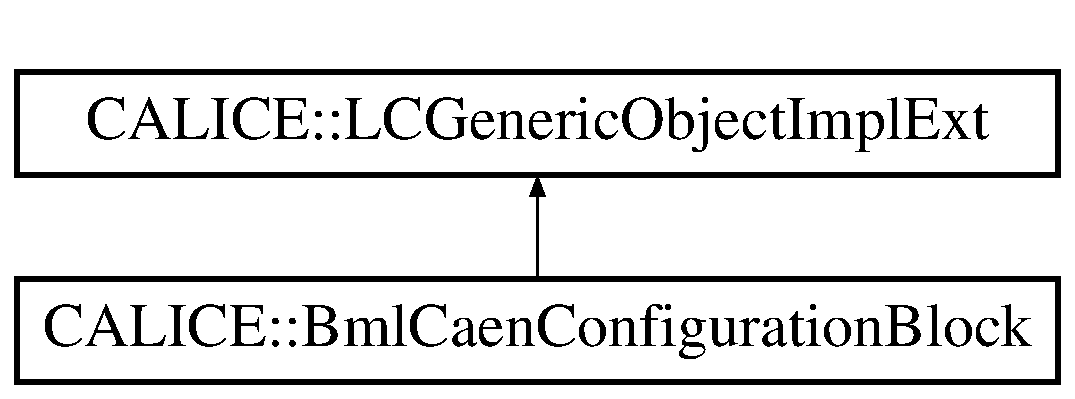
\includegraphics[height=2cm]{classCALICE_1_1BmlCaenConfigurationBlock}
\end{center}
\end{figure}
\subsection*{Public Member Functions}
\begin{DoxyCompactItemize}
\item 
{\bfseries BmlCaenConfigurationBlock} (LCObject $\ast$obj)\label{classCALICE_1_1BmlCaenConfigurationBlock_a15ef15c6db9d50ae58e65f2c98ed73bd}

\item 
{\bf BmlCaenConfigurationBlock} \& {\bfseries setBoardID} (int boardid)\label{classCALICE_1_1BmlCaenConfigurationBlock_a59fe78bec24532de95313aef863c9ff2}

\item 
int {\bfseries getBoardID} ()\label{classCALICE_1_1BmlCaenConfigurationBlock_a360a11a0204d58df71637193c4b9ead1}

\item 
{\bf BmlCaenConfigurationBlock} \& {\bfseries setBaseAddress} (int baseaddress)\label{classCALICE_1_1BmlCaenConfigurationBlock_a079fc5fd9026b0ef6c05fe33317290e9}

\item 
short {\bfseries getBaseAddress} () const \label{classCALICE_1_1BmlCaenConfigurationBlock_a8e7b031737715e85f55e8b4125d0b76b}

\item 
{\bf BmlCaenConfigurationBlock} \& {\bfseries setRecordLabel} (int label)\label{classCALICE_1_1BmlCaenConfigurationBlock_ac272a9c66fd223224a2a200cb7d2a66b}

\item 
short {\bfseries getRecordLabel} () const \label{classCALICE_1_1BmlCaenConfigurationBlock_aa8b83429f623d10f65edabe8a8b5a4a1}

\item 
{\bf BmlCaenConfigurationBlock} \& {\bfseries setControlRegister} (int controlregister)\label{classCALICE_1_1BmlCaenConfigurationBlock_adf3f1a86fc1b8e1088669ae247dc96a6}

\item 
int {\bfseries getControlRegister} ()\label{classCALICE_1_1BmlCaenConfigurationBlock_acbcca488fd13727aa889f6ad53c8f4dc}

\item 
{\bf BmlCaenConfigurationBlock} \& {\bfseries setInterruptRegister} (int interruptregister)\label{classCALICE_1_1BmlCaenConfigurationBlock_aebab0b05f74576366201b44bee1752a6}

\item 
int {\bfseries getInterruptRegister} ()\label{classCALICE_1_1BmlCaenConfigurationBlock_af4ee7799dca9ad03e3d214b1d736fa13}

\item 
{\bf BmlCaenConfigurationBlock} \& {\bfseries setCountRegister} (int countregister)\label{classCALICE_1_1BmlCaenConfigurationBlock_a49de9d6d4578e37f78362ca9be910cae}

\item 
int {\bfseries getCountRegister} ()\label{classCALICE_1_1BmlCaenConfigurationBlock_a4b63566dafbbe73c046ea94962f28c4d}

\item 
{\bf BmlCaenConfigurationBlock} \& {\bfseries setSpare} (int spare)\label{classCALICE_1_1BmlCaenConfigurationBlock_a25eafb2a9abb905b2fcea1395d735225}

\item 
int {\bfseries getSpare} ()\label{classCALICE_1_1BmlCaenConfigurationBlock_a56e1badfdaed4148f5c89c045a9d8e2f}

\item 
void {\bfseries print} (std::ostream \&os)\label{classCALICE_1_1BmlCaenConfigurationBlock_a68dbb32906d68303dad6b5f4a8ba35c2}

\item 
const std::string {\bfseries getTypeName} () const \label{classCALICE_1_1BmlCaenConfigurationBlock_ae6b54fef6a2a397b27237787b4c1ad24}

\item 
const std::string {\bfseries getDataDescription} () const \label{classCALICE_1_1BmlCaenConfigurationBlock_a8bd06c4d35fb60d77e1bedb3a53a3523}

\end{DoxyCompactItemize}


\subsection{Detailed Description}
Class to store configuration data of the Caen TDCs (767, 1290) Replaces BmlCaen767ConfigurationData. \begin{DoxyAuthor}{Author}
R.Poeschl (LAL Orsay) 
\end{DoxyAuthor}
\begin{DoxyDate}{Date}
Oct 31 2010 
\end{DoxyDate}


Definition at line 29 of file BmlCaenConfigurationBlock.hh.

The documentation for this class was generated from the following file:\begin{DoxyCompactItemize}
\item 
BmlCaenConfigurationBlock.hh\end{DoxyCompactItemize}

\section{CALICE::BmlEventData Class Reference}
\label{classCALICE_1_1BmlEventData}\index{CALICE::BmlEventData@{CALICE::BmlEventData}}


Class to store the \doxyref{BmlEventData}{p.}{classCALICE_1_1BmlEventData}.  


{\ttfamily \#include $<$BmlEventData.hh$>$}Inheritance diagram for CALICE::BmlEventData::\begin{figure}[H]
\begin{center}
\leavevmode
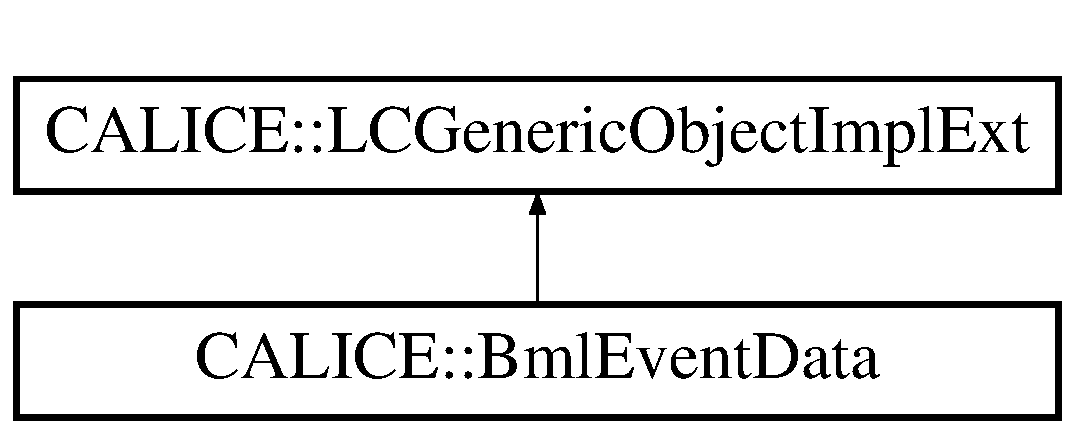
\includegraphics[height=2cm]{classCALICE_1_1BmlEventData}
\end{center}
\end{figure}
\subsection*{Public Member Functions}
\begin{DoxyCompactItemize}
\item 
{\bf BmlEventData} ()\label{classCALICE_1_1BmlEventData_aa67d8ecf7a32109b97c00cffd6ac68c3}

\begin{DoxyCompactList}\small\item\em Default Constructor. \item\end{DoxyCompactList}\item 
{\bf BmlEventData} (LCObject $\ast$obj)\label{classCALICE_1_1BmlEventData_a556af620c0b013022a16363eb93d72d6}

\begin{DoxyCompactList}\small\item\em A copy constructor. \item\end{DoxyCompactList}\item 
virtual {\bf $\sim$BmlEventData} ()\label{classCALICE_1_1BmlEventData_a465574a0d2cb1c9cec3cc9e0e543f7ae}

\begin{DoxyCompactList}\small\item\em The destructor. \item\end{DoxyCompactList}\item 
void {\bf addSupplementaryInformation} (LCEvent $\ast$aEvt, unsigned int ielm)
\begin{DoxyCompactList}\small\item\em Add supplementary information: Feed information not available in the actual \doxyref{BmlEventData}{p.}{classCALICE_1_1BmlEventData} to the object. \item\end{DoxyCompactList}\item 
{\bf BmlEventData} \& {\bf setBoardID} (int boardID)
\begin{DoxyCompactList}\small\item\em set the packed board id. \item\end{DoxyCompactList}\item 
int {\bf getBoardID} () const \label{classCALICE_1_1BmlEventData_a802624fa05776cd6430c6876ef65d950}

\begin{DoxyCompactList}\small\item\em get the board id \item\end{DoxyCompactList}\item 
{\bf BmlEventData} \& {\bf setBaseAddress} (int baseaddress)\label{classCALICE_1_1BmlEventData_afea25a27f1395bb140196b87c311d4a4}

\begin{DoxyCompactList}\small\item\em Set the Base Address of this TDC. \item\end{DoxyCompactList}\item 
short {\bf getBaseAddress} () const \label{classCALICE_1_1BmlEventData_a392737613082f9752a2c5e84a45e3201}

\begin{DoxyCompactList}\small\item\em Return the Base Address. \item\end{DoxyCompactList}\item 
{\bf BmlEventData} \& {\bf setRecordLabel} (int label)\label{classCALICE_1_1BmlEventData_acec730905f3fce6555d2f59fa5ba19cf}

\begin{DoxyCompactList}\small\item\em Set the Record Label. \item\end{DoxyCompactList}\item 
short {\bf getRecordLabel} () const \label{classCALICE_1_1BmlEventData_ae80cac54546f6f102f069414ed031c3d}

\begin{DoxyCompactList}\small\item\em Return the Record Label. \item\end{DoxyCompactList}\item 
{\bf BmlEventData} \& {\bf setStatusRegister} (int statreg)\label{classCALICE_1_1BmlEventData_aefe41281cd9af82a4a24c08d2ab1269b}

\begin{DoxyCompactList}\small\item\em Set the status register Value. \item\end{DoxyCompactList}\item 
int {\bf getStatusRegister} () const \label{classCALICE_1_1BmlEventData_a35bc6ad106c13c03be291494e19904b0}

\begin{DoxyCompactList}\small\item\em Get the status register value. \item\end{DoxyCompactList}\item 
{\bf BmlEventData} \& {\bf setNumberOfWords} (int numwords)\label{classCALICE_1_1BmlEventData_a7aee8d1aad0f8fe7e2489362a17085be}

\begin{DoxyCompactList}\small\item\em Set the number of words. \item\end{DoxyCompactList}\item 
int {\bf getNumberOfWords} () const \label{classCALICE_1_1BmlEventData_a62adde679450ee19364121aabe84b419}

\begin{DoxyCompactList}\small\item\em Get the number of words. \item\end{DoxyCompactList}\item 
{\bf BmlEventData} \& {\bf setGeoAddress} (int geoaddress)\label{classCALICE_1_1BmlEventData_a7932d1fb4d2ee46a8e99cd37967b2b4c}

\begin{DoxyCompactList}\small\item\em Set the geo Address of the TDC. \item\end{DoxyCompactList}\item 
int {\bf getGeoAddress} () const \label{classCALICE_1_1BmlEventData_a10e6df6233068413112a80f2019aabc0}

\begin{DoxyCompactList}\small\item\em Get the geo Address. \item\end{DoxyCompactList}\item 
{\bf BmlEventData} \& {\bf setEventNumber} (int eventnumber)\label{classCALICE_1_1BmlEventData_a860cacaab0517981c00347d202237120}

\begin{DoxyCompactList}\small\item\em Set the event number as counted by the TDC. \item\end{DoxyCompactList}\item 
int {\bf getEventNumber} () const \label{classCALICE_1_1BmlEventData_a82cf900eb42abb77da0a0e85c6a9968f}

\begin{DoxyCompactList}\small\item\em Get the event Number. \item\end{DoxyCompactList}\item 
{\bf BmlEventData} \& {\bf setStatus} (int status)\label{classCALICE_1_1BmlEventData_a9f65a78e21ff2816ba4fbe96ef240bd9}

\begin{DoxyCompactList}\small\item\em Set status as present when the the eob record appears. \item\end{DoxyCompactList}\item 
int {\bf getStatus} () const \label{classCALICE_1_1BmlEventData_a30f49cce27697fb66ad59add06094e35}

\begin{DoxyCompactList}\small\item\em Get the status value. \item\end{DoxyCompactList}\item 
{\bf BmlEventData} \& {\bf setEventDataCounter} (int evtdatacounter)\label{classCALICE_1_1BmlEventData_aabf7d25451c61875c4dde0f33a33f366}

\begin{DoxyCompactList}\small\item\em Set the EventData counter as present when the the eob record appears. \item\end{DoxyCompactList}\item 
int {\bf getEventDataCounter} () const \label{classCALICE_1_1BmlEventData_a22685cc5c125541fd7dff408bf11a6ea}

\begin{DoxyCompactList}\small\item\em Get the event data counter value. \item\end{DoxyCompactList}\item 
int {\bf getNumberOfSignalChannels} () const \label{classCALICE_1_1BmlEventData_a1142020abee10914560bf8eba80b6225}

\begin{DoxyCompactList}\small\item\em Get the number of channels which carry a signal. \item\end{DoxyCompactList}\item 
{\bf BmlEventData} \& {\bf setTDCType} (std::string typeStr)
\begin{DoxyCompactList}\small\item\em Here follow the setting and getting of the information from the class holding supplementary information. \item\end{DoxyCompactList}\item 
std::string {\bf getTDCType} ()\label{classCALICE_1_1BmlEventData_a816f61c11888b918a14dad1fc9301c7e}

\begin{DoxyCompactList}\small\item\em retrieve the typename \item\end{DoxyCompactList}\item 
{\bf BmlEventData} \& {\bf setEventFifoCont} (int fifocont)
\begin{DoxyCompactList}\small\item\em set the Fifo Cont id. \item\end{DoxyCompactList}\item 
unsigned short {\bf getWordCount} ()\label{classCALICE_1_1BmlEventData_a2a65e16561e4df0b260561713e982c8d}

\begin{DoxyCompactList}\small\item\em get the word count \item\end{DoxyCompactList}\item 
unsigned short {\bf getEventCount} ()\label{classCALICE_1_1BmlEventData_af1fce77ca4743c7733dfe0952f960244}

\begin{DoxyCompactList}\small\item\em get the event count \item\end{DoxyCompactList}\item 
{\bf BmlEventData} \& {\bf setBunchID} (int bunchID)
\begin{DoxyCompactList}\small\item\em set the bunch id. \item\end{DoxyCompactList}\item 
unsigned int {\bf getBunchID} ()\label{classCALICE_1_1BmlEventData_a2768e6cfbde1495d057a6cd36e581a3b}

\begin{DoxyCompactList}\small\item\em get the bunch id \item\end{DoxyCompactList}\item 
{\bf BmlEventData} \& {\bf setEventIDTrailer} (int eventIDTrailer)\label{classCALICE_1_1BmlEventData_a527c6d1ba7a7e575f16dd95a5b5c198b}

\begin{DoxyCompactList}\small\item\em Set the eventid from the TDC trailer. \item\end{DoxyCompactList}\item 
unsigned int {\bf getEventIDTrailer} ()\label{classCALICE_1_1BmlEventData_a7e5b77a0457590fad53a5983ea7c7e7b}

\begin{DoxyCompactList}\small\item\em get the event id trailer \item\end{DoxyCompactList}\item 
{\bf BmlEventData} \& {\bf setTDCErrors} (int tdcErrors)\label{classCALICE_1_1BmlEventData_a7d3195e0c08976bfc5e1122efea915cf}

\begin{DoxyCompactList}\small\item\em Set the TDC errors. \item\end{DoxyCompactList}\item 
unsigned int {\bf getTDCErrors} ()\label{classCALICE_1_1BmlEventData_a30e07f8dc96ecb2aadac9606dbf9b4f9}

\begin{DoxyCompactList}\small\item\em get the tdc errors \item\end{DoxyCompactList}\item 
{\bf BmlEventData} \& {\bf setBufferOverflow} (int bufferOverflow)\label{classCALICE_1_1BmlEventData_a03eecee3ea4ae146c3320caee9ba813f}

\begin{DoxyCompactList}\small\item\em Set the buffer overflow. \item\end{DoxyCompactList}\item 
unsigned int {\bf getBufferOverflow} ()\label{classCALICE_1_1BmlEventData_a42a5c16c75f78d794441830c9eae1cb7}

\begin{DoxyCompactList}\small\item\em get the buffer overflow \item\end{DoxyCompactList}\item 
{\bf BmlEventData} \& {\bf setTriggerLost} (int triggerlost)\label{classCALICE_1_1BmlEventData_ae97639de2ca13acb95d0cbbef7d51b7a}

\begin{DoxyCompactList}\small\item\em Set the number of words in the trailer. \item\end{DoxyCompactList}\item 
unsigned int {\bf getTriggerLost} ()\label{classCALICE_1_1BmlEventData_a1a250cc192a3874ca587efd9712bc27c}

\begin{DoxyCompactList}\small\item\em Get information on lost triggers. \item\end{DoxyCompactList}\item 
{\bf BmlEventData} \& {\bf setTDCWordCountTrailer} (int numwords)\label{classCALICE_1_1BmlEventData_a37546da528d855946dfc12faa2a836d4}

\begin{DoxyCompactList}\small\item\em Set the number of words in the trailer. \item\end{DoxyCompactList}\item 
unsigned int {\bf getTDCWordCountTrailer} ()\label{classCALICE_1_1BmlEventData_a16022acb74c6d58f32ea5388a16ed752}

\begin{DoxyCompactList}\small\item\em Get the number of words in the trailer. \item\end{DoxyCompactList}\item 
{\bf BmlEventDataSup} $\ast$ {\bf getSupObject} ()\label{classCALICE_1_1BmlEventData_ab7a136495e35b3c0d9ce8e14052b7a38}

\begin{DoxyCompactList}\small\item\em return the supplementary object \item\end{DoxyCompactList}\item 
void {\bf addTDCChannels} (const TDCChannelContainer\_\-t \&)
\begin{DoxyCompactList}\small\item\em Get measurements for each tdc channel The data are stored at the end of the collection with the following 'protocol' channelnumber number of signals m startime word, i.e. \item\end{DoxyCompactList}\item 
const TDCChannelContainer\_\-t \& {\bf getTDCChannelContainer} ()
\begin{DoxyCompactList}\small\item\em Returns a container with tdc channel info The first part of the map is the channelnumber The second part of the map is a pair consisting of an indicator whether the measurement is a starttime and the actual time measurement (the core of it all) falling egdes are indicated by a minus sign. \item\end{DoxyCompactList}\item 
const std::string {\bf getTypeName} () const \label{classCALICE_1_1BmlEventData_a7113442068c692c4a4734204006d1801}

\begin{DoxyCompactList}\small\item\em returns the the type name \item\end{DoxyCompactList}\item 
const std::string {\bf getDataDescription} () const \label{classCALICE_1_1BmlEventData_ab525cda04a44662b1054fa7d52729e41}

\begin{DoxyCompactList}\small\item\em returns a brief description of the data stored \item\end{DoxyCompactList}\item 
std::ostream \& {\bf print} (std::ostream \&ostrm)\label{classCALICE_1_1BmlEventData_aef388c90f9b4060f6a14ae4c95cea7f8}

\begin{DoxyCompactList}\small\item\em dumps data content \item\end{DoxyCompactList}\item 
void {\bf printInitWarning} ()\label{classCALICE_1_1BmlEventData_a4ce6ef2fedee15aa6a22b9efcf2ef47a}

\begin{DoxyCompactList}\small\item\em A convenient method which prints a warning in case the supplementary information is not initialiasied. \item\end{DoxyCompactList}\end{DoxyCompactItemize}
\subsection*{Private Member Functions}
\begin{DoxyCompactItemize}
\item 
void {\bf setNumberOfSignalChannels} (int numsig)\label{classCALICE_1_1BmlEventData_a06db71a4d74f2161e9ed473b40a201c4}

\begin{DoxyCompactList}\small\item\em Set the number of channels which carry a signal. \item\end{DoxyCompactList}\end{DoxyCompactItemize}
\subsection*{Private Attributes}
\begin{DoxyCompactItemize}
\item 
TDCChannelContainer\_\-t {\bf \_\-tdcChannelContainer}\label{classCALICE_1_1BmlEventData_a07eed0229a50826d0f7971ce63908ff5}

\begin{DoxyCompactList}\small\item\em The channel container which we will return to the user. \item\end{DoxyCompactList}\item 
bool {\bf \_\-isSupInitialised}\label{classCALICE_1_1BmlEventData_af07d35f6779f05e1cd8a6250ea04f03c}

\begin{DoxyCompactList}\small\item\em A bool deciding whether supplementary object has been correctly created. \item\end{DoxyCompactList}\end{DoxyCompactItemize}
\subsection*{Static Private Attributes}
\begin{DoxyCompactItemize}
\item 
static {\bf BmlEventDataSup} $\ast$ {\bf \_\-bml\_\-event\_\-sup} = 0\label{classCALICE_1_1BmlEventData_a3bfbc46119fcbaf3021a151bbd6f0dfc}

\begin{DoxyCompactList}\small\item\em An object of the associated class. \item\end{DoxyCompactList}\item 
static bool {\bf \_\-isWarning1Printed} = false\label{classCALICE_1_1BmlEventData_a1db181ffb9adbb6f490bcb71eb8e16e4}

\begin{DoxyCompactList}\small\item\em A bool which prevents prohibitive numerous printing of warnings. \item\end{DoxyCompactList}\item 
static bool {\bf \_\-isWarning2Printed} = false\label{classCALICE_1_1BmlEventData_afd1b9ffb350aa39b5efb380320126b9d}

\begin{DoxyCompactList}\small\item\em Another bool which prevents prohibitive numerous printing of warnings. \item\end{DoxyCompactList}\item 
static bool {\bf \_\-isWarning3Printed} = false\label{classCALICE_1_1BmlEventData_af0ef4c5411a8bfba056415651686a8f2}

\begin{DoxyCompactList}\small\item\em Yet Another bool which prevents prohibitive numerous printing of warnings. \item\end{DoxyCompactList}\end{DoxyCompactItemize}


\subsection{Detailed Description}
Class to store the \doxyref{BmlEventData}{p.}{classCALICE_1_1BmlEventData}. This is tailored to the data extracted from the Caen767 TDC. \begin{DoxyAuthor}{Author}
R. P�schl (LAL Orsay) 
\end{DoxyAuthor}
\begin{DoxyDate}{Date}
Jul 24 2006 
\end{DoxyDate}


Definition at line 61 of file BmlEventData.hh.

\subsection{Member Function Documentation}
\index{CALICE::BmlEventData@{CALICE::BmlEventData}!addSupplementaryInformation@{addSupplementaryInformation}}
\index{addSupplementaryInformation@{addSupplementaryInformation}!CALICE::BmlEventData@{CALICE::BmlEventData}}
\subsubsection[{addSupplementaryInformation}]{\setlength{\rightskip}{0pt plus 5cm}void CALICE::BmlEventData::addSupplementaryInformation (LCEvent $\ast$ {\em aEvt}, \/  unsigned int {\em ielm})\hspace{0.3cm}{\ttfamily  [inline]}}\label{classCALICE_1_1BmlEventData_a8092124f2b78b59f656337647f359c27}


Add supplementary information: Feed information not available in the actual \doxyref{BmlEventData}{p.}{classCALICE_1_1BmlEventData} to the object. This is necessary to handle more than 1 TDC type, in fact all information from TDCs others than the Caen767 will be handled as supplementary information, this ensures full backward compatibility and requires minimal code changes if information from other TDC is requested. 

Definition at line 106 of file BmlEventData.hh.

References \_\-bml\_\-event\_\-sup, \_\-isSupInitialised, and \_\-isWarning3Printed.\index{CALICE::BmlEventData@{CALICE::BmlEventData}!addTDCChannels@{addTDCChannels}}
\index{addTDCChannels@{addTDCChannels}!CALICE::BmlEventData@{CALICE::BmlEventData}}
\subsubsection[{addTDCChannels}]{\setlength{\rightskip}{0pt plus 5cm}void CALICE::BmlEventData::addTDCChannels (const TDCChannelContainer\_\-t \& {\em tdcChannelContainer})}\label{classCALICE_1_1BmlEventData_acb448530583ebab240c3d50efe72bc3d}


Get measurements for each tdc channel The data are stored at the end of the collection with the following 'protocol' channelnumber number of signals m startime word, i.e. each measurement occupies one bit in this word signal 1 ... signal m 

Definition at line 11 of file BmlEventData.cc.

References CALICE::LCGenericObjectImplExt::obj(), and setNumberOfSignalChannels().\index{CALICE::BmlEventData@{CALICE::BmlEventData}!getTDCChannelContainer@{getTDCChannelContainer}}
\index{getTDCChannelContainer@{getTDCChannelContainer}!CALICE::BmlEventData@{CALICE::BmlEventData}}
\subsubsection[{getTDCChannelContainer}]{\setlength{\rightskip}{0pt plus 5cm}const TDCChannelContainer\_\-t \& CALICE::BmlEventData::getTDCChannelContainer ()}\label{classCALICE_1_1BmlEventData_a9ba0b84d7d9ab8b5728a2cba1fa9f151}


Returns a container with tdc channel info The first part of the map is the channelnumber The second part of the map is a pair consisting of an indicator whether the measurement is a starttime and the actual time measurement (the core of it all) falling egdes are indicated by a minus sign. A method which re-\/builds and returns the TCChannelContainer. 

Definition at line 52 of file BmlEventData.cc.

References \_\-tdcChannelContainer, and getNumberOfSignalChannels().

Referenced by print().\index{CALICE::BmlEventData@{CALICE::BmlEventData}!setBoardID@{setBoardID}}
\index{setBoardID@{setBoardID}!CALICE::BmlEventData@{CALICE::BmlEventData}}
\subsubsection[{setBoardID}]{\setlength{\rightskip}{0pt plus 5cm}{\bf BmlEventData}\& CALICE::BmlEventData::setBoardID (int {\em boardID})\hspace{0.3cm}{\ttfamily  [inline]}}\label{classCALICE_1_1BmlEventData_a87da8c5f50787e64485afd71f870d4d4}


set the packed board id. \begin{DoxySeeAlso}{See also}
\doxyref{BoardID}{p.}{classCALICE_1_1BoardID} For the Caen 767 TDC the boardID has a slightly different meaning compared with the CrcBoards slotID and board component numbers are just the MSB and LSB of the base address. 
\end{DoxySeeAlso}


Definition at line 133 of file BmlEventData.hh.

References CALICE::LCGenericObjectImplExt::obj().

Referenced by BmlEventData().\index{CALICE::BmlEventData@{CALICE::BmlEventData}!setBunchID@{setBunchID}}
\index{setBunchID@{setBunchID}!CALICE::BmlEventData@{CALICE::BmlEventData}}
\subsubsection[{setBunchID}]{\setlength{\rightskip}{0pt plus 5cm}{\bf BmlEventData}\& CALICE::BmlEventData::setBunchID (int {\em bunchID})\hspace{0.3cm}{\ttfamily  [inline]}}\label{classCALICE_1_1BmlEventData_ae86922e82f92fbb4018d4ce257971fc0}


set the bunch id. 

Definition at line 287 of file BmlEventData.hh.

References \_\-bml\_\-event\_\-sup, and CALICE::BmlEventDataSup::setBunchID().\index{CALICE::BmlEventData@{CALICE::BmlEventData}!setEventFifoCont@{setEventFifoCont}}
\index{setEventFifoCont@{setEventFifoCont}!CALICE::BmlEventData@{CALICE::BmlEventData}}
\subsubsection[{setEventFifoCont}]{\setlength{\rightskip}{0pt plus 5cm}{\bf BmlEventData}\& CALICE::BmlEventData::setEventFifoCont (int {\em fifocont})\hspace{0.3cm}{\ttfamily  [inline]}}\label{classCALICE_1_1BmlEventData_a26c3ac15a946f233f4c27cae463f18ad}


set the Fifo Cont id. 

Definition at line 261 of file BmlEventData.hh.

References \_\-bml\_\-event\_\-sup, and CALICE::BmlEventDataSup::setEventFifoCont().\index{CALICE::BmlEventData@{CALICE::BmlEventData}!setTDCType@{setTDCType}}
\index{setTDCType@{setTDCType}!CALICE::BmlEventData@{CALICE::BmlEventData}}
\subsubsection[{setTDCType}]{\setlength{\rightskip}{0pt plus 5cm}{\bf BmlEventData}\& CALICE::BmlEventData::setTDCType (std::string {\em typeStr})\hspace{0.3cm}{\ttfamily  [inline]}}\label{classCALICE_1_1BmlEventData_a9355f03a743f43801ce6d4db6e5fffe1}


Here follow the setting and getting of the information from the class holding supplementary information. set the TDC type 

Definition at line 241 of file BmlEventData.hh.

References \_\-bml\_\-event\_\-sup, and CALICE::BmlEventDataSup::setTDCType().

The documentation for this class was generated from the following files:\begin{DoxyCompactItemize}
\item 
BmlEventData.hh\item 
BmlEventData.cc\end{DoxyCompactItemize}

\section{CALICE::BmlEventDataSup Class Reference}
\label{classCALICE_1_1BmlEventDataSup}\index{CALICE::BmlEventDataSup@{CALICE::BmlEventDataSup}}


Class to store supplementary \doxyref{BmlEventData}{p.}{classCALICE_1_1BmlEventData}.  


{\ttfamily \#include $<$BmlEventDataSup.hh$>$}Inheritance diagram for CALICE::BmlEventDataSup::\begin{figure}[H]
\begin{center}
\leavevmode
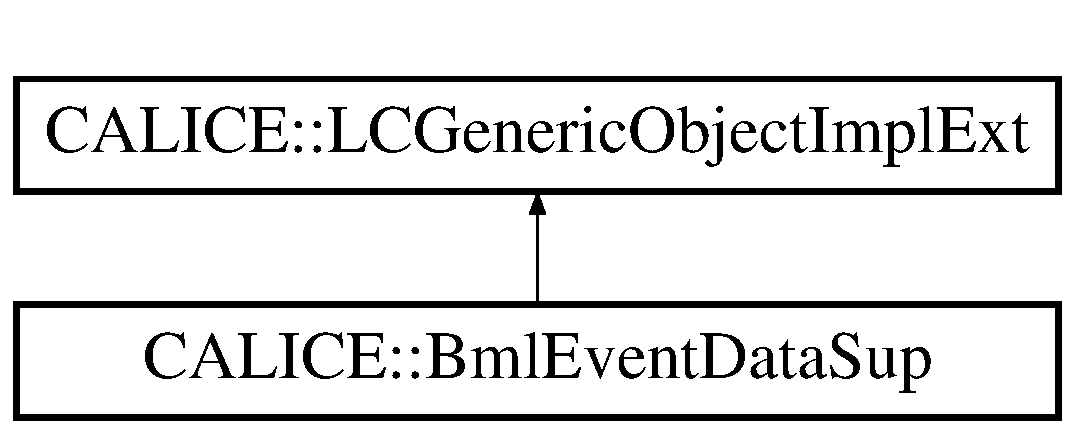
\includegraphics[height=2cm]{classCALICE_1_1BmlEventDataSup}
\end{center}
\end{figure}
\subsection*{Private Member Functions}
\begin{DoxyCompactItemize}
\item 
{\bf BmlEventDataSup} ()\label{classCALICE_1_1BmlEventDataSup_a1b777ba65db201936af16ba56dc197de}

\begin{DoxyCompactList}\small\item\em Default Constructor. \item\end{DoxyCompactList}\item 
{\bf BmlEventDataSup} (LCObject $\ast$obj)\label{classCALICE_1_1BmlEventDataSup_ababa5fa292e17ad8181dd30149f4d87e}

\begin{DoxyCompactList}\small\item\em A copy constructor. \item\end{DoxyCompactList}\item 
virtual {\bf $\sim$BmlEventDataSup} ()\label{classCALICE_1_1BmlEventDataSup_a8b5715bd0afdd93a7a5573bede6c047a}

\begin{DoxyCompactList}\small\item\em The destructor. \item\end{DoxyCompactList}\item 
{\bf BmlEventDataSup} \& {\bf setTDCType} (std::string typeStr)
\begin{DoxyCompactList}\small\item\em set the tdc type \item\end{DoxyCompactList}\item 
void {\bfseries setPointerToIndexOfIntTypeNames} (int nameind)\label{classCALICE_1_1BmlEventDataSup_a9fa4191baf23435b722322fb1ca8b56e}

\item 
void {\bfseries setLengthIndexOfIntTypeNames} (int lengthindex)\label{classCALICE_1_1BmlEventDataSup_ad5cfea715dbde1072b8c8a47f61c656e}

\item 
int {\bf getLengthIndexOfIntTypeNames} () const \label{classCALICE_1_1BmlEventDataSup_a21ebe68dd1e819533a2af15879b1653d}

\begin{DoxyCompactList}\small\item\em Retrieve the index at which the lengths of the names of the int data types do start. \item\end{DoxyCompactList}\item 
int {\bf getPointerToIndexOfIntTypeNames} () const \label{classCALICE_1_1BmlEventDataSup_afc31491a2fe74e80c3bf4b98b1a6ec1c}

\begin{DoxyCompactList}\small\item\em Retrieve the index at which the pointer to the names of int data types do start. \item\end{DoxyCompactList}\item 
void {\bf setTypeIndex} (int pos, int value)\label{classCALICE_1_1BmlEventDataSup_afeadf8495ac708b6eb4f372e262b4115}

\begin{DoxyCompactList}\small\item\em Set the index of a given data type name. \item\end{DoxyCompactList}\item 
std::string {\bf getTDCType} () const 
\begin{DoxyCompactList}\small\item\em get the tdc type \item\end{DoxyCompactList}\item 
{\bf BmlEventDataSup} \& {\bf setEventFifoCont} (int fifocont)\label{classCALICE_1_1BmlEventDataSup_ac3263e6f4c8a3be3b1ca36308b0f32c8}

\begin{DoxyCompactList}\small\item\em Store the FIFO content. \item\end{DoxyCompactList}\item 
unsigned short {\bf getEventCount} () const \label{classCALICE_1_1BmlEventDataSup_a1284d5d9b342180a65d3aef2cd593a50}

\begin{DoxyCompactList}\small\item\em get the event count \item\end{DoxyCompactList}\item 
unsigned short {\bf getWordCount} () const \label{classCALICE_1_1BmlEventDataSup_a75f899e45c6c056103e25fce6acb0851}

\begin{DoxyCompactList}\small\item\em get the word count \item\end{DoxyCompactList}\item 
{\bf BmlEventDataSup} \& {\bf setBunchID} (int bunchid)\label{classCALICE_1_1BmlEventDataSup_acef67a0bc90854904fb4382501ecaf8d}

\begin{DoxyCompactList}\small\item\em set the bunch id \item\end{DoxyCompactList}\item 
int {\bf getBunchID} () const \label{classCALICE_1_1BmlEventDataSup_a402a35429e1fb4cefc030246d6a7dc8d}

\begin{DoxyCompactList}\small\item\em get the bunch id \item\end{DoxyCompactList}\item 
{\bf BmlEventDataSup} \& {\bf setEventIDTrailer} (int eventIDTrailer)\label{classCALICE_1_1BmlEventDataSup_ac1a762c3a809585cb908e1f9edce15ac}

\begin{DoxyCompactList}\small\item\em Set the eventid from the TDC trailer. \item\end{DoxyCompactList}\item 
short {\bf getEventIDTrailer} () const \label{classCALICE_1_1BmlEventDataSup_af98ba50b8fb39a943bc35067ffaf337b}

\begin{DoxyCompactList}\small\item\em Return the eventid from the TDC trailer. \item\end{DoxyCompactList}\item 
{\bf BmlEventDataSup} \& {\bf setTDCErrors} (int tdcErrors)\label{classCALICE_1_1BmlEventDataSup_a812f9190cf1962203e1588669fc98f25}

\begin{DoxyCompactList}\small\item\em Set the TDC errors. \item\end{DoxyCompactList}\item 
int {\bf getTDCErrors} () const \label{classCALICE_1_1BmlEventDataSup_a53367b022e3100a0e3bd613ef2b70935}

\begin{DoxyCompactList}\small\item\em Get the TDC errors. \item\end{DoxyCompactList}\item 
{\bf BmlEventDataSup} \& {\bf setBufferOverflow} (int bufferOverflow)\label{classCALICE_1_1BmlEventDataSup_a90c7ac60defd7bb8a827f1aea40aedc6}

\begin{DoxyCompactList}\small\item\em Set the buffer overflow. \item\end{DoxyCompactList}\item 
int {\bf getBufferOverflow} () const \label{classCALICE_1_1BmlEventDataSup_a5d6652dad161f253768ae01418d2c669}

\begin{DoxyCompactList}\small\item\em Get the buffer overflow. \item\end{DoxyCompactList}\item 
{\bf BmlEventDataSup} \& {\bf setTriggerLost} (int triggerlost)\label{classCALICE_1_1BmlEventDataSup_ad432619ccacb13abb181a12ab4662822}

\begin{DoxyCompactList}\small\item\em Set the number of words in the trailer. \item\end{DoxyCompactList}\item 
int {\bf getTriggerLost} () const \label{classCALICE_1_1BmlEventDataSup_a7110357892a453499f8e3bbd2b0ff535}

\begin{DoxyCompactList}\small\item\em Get the number of lost triggers. \item\end{DoxyCompactList}\item 
{\bf BmlEventDataSup} \& {\bf setTDCWordCountTrailer} (int numwords)\label{classCALICE_1_1BmlEventDataSup_aa8e12d29d2060db9c3657a6e4f9d8ac7}

\begin{DoxyCompactList}\small\item\em Set the number of lost triggers. \item\end{DoxyCompactList}\item 
int {\bf getTDCWordCountTrailer} () const \label{classCALICE_1_1BmlEventDataSup_a688bc2f933ce1011e4a03ca904539f3c}

\begin{DoxyCompactList}\small\item\em Get the number of words in the trailer. \item\end{DoxyCompactList}\item 
const std::string {\bf getTypeName} () const \label{classCALICE_1_1BmlEventDataSup_a075786d44470d270e1e931bcfa896394}

\begin{DoxyCompactList}\small\item\em returns the the type name \item\end{DoxyCompactList}\item 
const std::string {\bf getDataDescription} () const \label{classCALICE_1_1BmlEventDataSup_acebe6fba59eced039cc6bad225e9bc71}

\begin{DoxyCompactList}\small\item\em returns a brief description of the data stored \item\end{DoxyCompactList}\item 
std::ostream \& {\bf print} (std::ostream \&ostrmsup)\label{classCALICE_1_1BmlEventDataSup_ae4684c1d74d640dd5b4258d1af5d2e70}

\begin{DoxyCompactList}\small\item\em dumps data content \item\end{DoxyCompactList}\end{DoxyCompactItemize}
\subsection*{Friends}
\begin{DoxyCompactItemize}
\item 
class {\bfseries BmlEventData}\label{classCALICE_1_1BmlEventDataSup_af03b3108e540123cf6fb29facde51e29}

\end{DoxyCompactItemize}


\subsection{Detailed Description}
Class to store supplementary \doxyref{BmlEventData}{p.}{classCALICE_1_1BmlEventData}. This is tailored to the data extracted from the Caen TDCs in extension of the actual class \doxyref{BmlEventData}{p.}{classCALICE_1_1BmlEventData} This class is written such that it should be only accessed via the aforementioned class The user is strongly discouraged to instantiate by him/herself. It has only private functions and declares \doxyref{BmlEventData}{p.}{classCALICE_1_1BmlEventData} to be its friend. \begin{DoxyAuthor}{Author}
R. P�schl (LAL Orsay) 
\end{DoxyAuthor}
\begin{DoxyDate}{Date}
Oct 13 2010 
\end{DoxyDate}


Definition at line 52 of file BmlEventDataSup.hh.

\subsection{Member Function Documentation}
\index{CALICE::BmlEventDataSup@{CALICE::BmlEventDataSup}!getTDCType@{getTDCType}}
\index{getTDCType@{getTDCType}!CALICE::BmlEventDataSup@{CALICE::BmlEventDataSup}}
\subsubsection[{getTDCType}]{\setlength{\rightskip}{0pt plus 5cm}std::string CALICE::BmlEventDataSup::getTDCType () const\hspace{0.3cm}{\ttfamily  [inline, private]}}\label{classCALICE_1_1BmlEventDataSup_a2e28417799fb6b46b4fd5bd798bffed3}


get the tdc type Currently since only one string in object -\/$>$ to be modified if more strings 

Definition at line 144 of file BmlEventDataSup.hh.

References getLengthIndexOfIntTypeNames(), getPointerToIndexOfIntTypeNames(), and CALICE::getStringFromInts().

Referenced by CALICE::BmlEventData::getTDCType(), and print().\index{CALICE::BmlEventDataSup@{CALICE::BmlEventDataSup}!setTDCType@{setTDCType}}
\index{setTDCType@{setTDCType}!CALICE::BmlEventDataSup@{CALICE::BmlEventDataSup}}
\subsubsection[{setTDCType}]{\setlength{\rightskip}{0pt plus 5cm}{\bf BmlEventDataSup}\& CALICE::BmlEventDataSup::setTDCType (std::string {\em typeStr})\hspace{0.3cm}{\ttfamily  [inline, private]}}\label{classCALICE_1_1BmlEventDataSup_ab3677309acfd81396e1333ff9b967f2a}


set the tdc type 

Store the index at which the pointer to the names of the int data data types do start

This written such that it can be extended in case more strings need to be stored

Would however trigger a bit of re-\/writing but at least it \_\-sure\_\- that it remains always

compatible and flexible

We use the same ugly but successful technique as in \doxyref{DaqTypeDataBlock}{p.}{classCALICE_1_1DaqTypeDataBlock} (we may even be able to inherit from it

now we've simply copied a few useful methods -\/$>$ to be checked 

Definition at line 94 of file BmlEventDataSup.hh.

References CALICE::convertStringToInts(), getLengthIndexOfIntTypeNames(), getPointerToIndexOfIntTypeNames(), CALICE::LCGenericObjectImplExt::obj(), and setTypeIndex().

Referenced by BmlEventDataSup(), and CALICE::BmlEventData::setTDCType().

The documentation for this class was generated from the following files:\begin{DoxyCompactItemize}
\item 
BmlEventDataSup.hh\item 
BmlEventDataSup.cc\end{DoxyCompactItemize}

\section{CALICE::BmlSlowRunDataBlock Class Reference}
\label{classCALICE_1_1BmlSlowRunDataBlock}\index{CALICE::BmlSlowRunDataBlock@{CALICE::BmlSlowRunDataBlock}}


Interface Class to access the BmlSlowRun Data Here we handle ahc voltages, temperatures et al.  


{\ttfamily \#include $<$BmlSlowRunDataBlock.hh$>$}Inheritance diagram for CALICE::BmlSlowRunDataBlock::\begin{figure}[H]
\begin{center}
\leavevmode
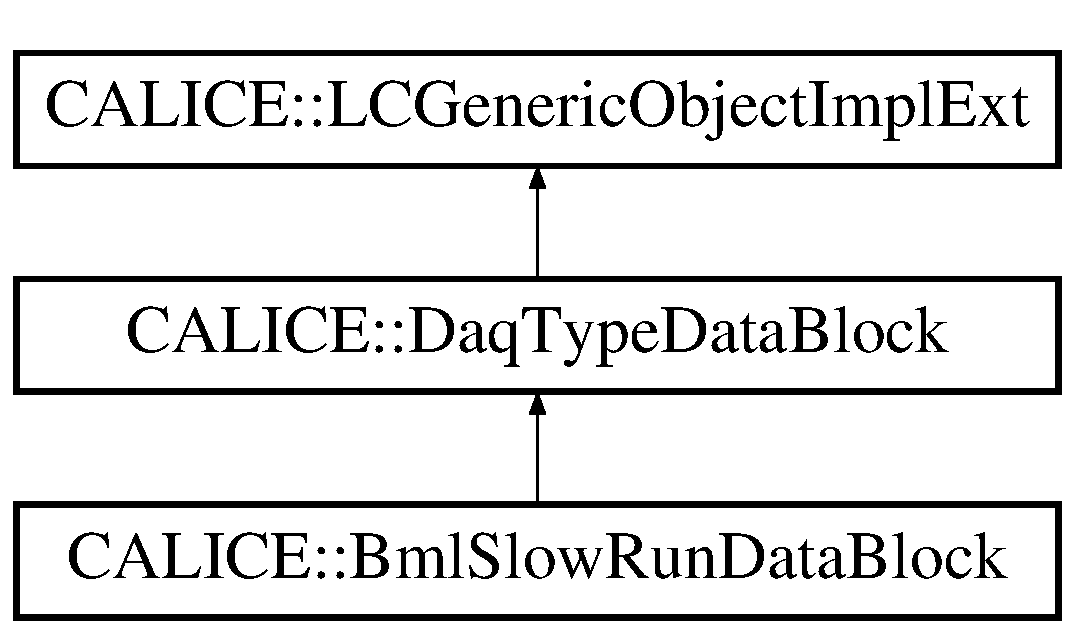
\includegraphics[height=3cm]{classCALICE_1_1BmlSlowRunDataBlock}
\end{center}
\end{figure}
\subsection*{Public Member Functions}
\begin{DoxyCompactItemize}
\item 
{\bf BmlSlowRunDataBlock} ()\label{classCALICE_1_1BmlSlowRunDataBlock_a25c7a935d4873ff7065def913bf1c77c}

\begin{DoxyCompactList}\small\item\em Constructor. \item\end{DoxyCompactList}\item 
{\bf BmlSlowRunDataBlock} (LCObject $\ast$obj)\label{classCALICE_1_1BmlSlowRunDataBlock_ae4960ae7344e47dd4061e4a97067cce9}

\begin{DoxyCompactList}\small\item\em 'Copy constructor' needed to interpret LCCollection read from file/database. \item\end{DoxyCompactList}\item 
{\bf BmlSlowRunDataBlock} \& {\bf setAbsorberPosition} (double abspos)
\begin{DoxyCompactList}\small\item\em Store the aborber position device in cern h6b beamline to purify beam, ie. \item\end{DoxyCompactList}\item 
double {\bf getAbsorberPosition} () const \label{classCALICE_1_1BmlSlowRunDataBlock_a2eeaa6e8341b068b991d1c7ec42a0e8c}

\begin{DoxyCompactList}\small\item\em Retrieve the absorber position. \item\end{DoxyCompactList}\item 
{\bf BmlSlowRunDataBlock} \& {\bf setTimeStamp} (struct tm $\ast$timestamp)\label{classCALICE_1_1BmlSlowRunDataBlock_aaeaa4c4d05400ff8e10dca94acde6b5d}

\begin{DoxyCompactList}\small\item\em Sets the time stamp We store Year, Month, Day and Hour, Minute, Second We store UTC!!!! \item\end{DoxyCompactList}\item 
LCTime {\bf getTimeStamp} () const \label{classCALICE_1_1BmlSlowRunDataBlock_ae4bf5b8cb65578245c68add8a874e5a4}

\begin{DoxyCompactList}\small\item\em returns the start stamp \item\end{DoxyCompactList}\item 
LCTime {\bf getTimeStampBml} ()\label{classCALICE_1_1BmlSlowRunDataBlock_aa8e2d5f73a3ee0de0c6a0ebd972b4f23}

\begin{DoxyCompactList}\small\item\em Implementation of the method to obtain the timestamp as given by the beamline operators here identical to the only timestamp which was stored. \item\end{DoxyCompactList}\item 
LCTime {\bf getTimeStampDaq} ()\label{classCALICE_1_1BmlSlowRunDataBlock_a04c8788e599ae8873d81b515d67c9f93}

\begin{DoxyCompactList}\small\item\em Implementation of the method to obtain the timestamp as given by the calice daq Here 0 as no timestamp has been stored. \item\end{DoxyCompactList}\item 
{\bf BmlSlowRunDataBlock} \& {\bf setT4Position} (double t4pos)\label{classCALICE_1_1BmlSlowRunDataBlock_ac16185be4c02fc71f31e8773bebc9e19}

\begin{DoxyCompactList}\small\item\em Store the t4 position device in cern h6b beamline to produce desired particles out of the secondary beam. \item\end{DoxyCompactList}\item 
double {\bf getT4Position} () const \label{classCALICE_1_1BmlSlowRunDataBlock_a608e9bbb5084e0960e608fd9b3ece877}

\begin{DoxyCompactList}\small\item\em Retrieve the absorber position. \item\end{DoxyCompactList}\item 
{\bf BmlSlowRunDataBlock} \& {\bf setTargetPosition} (double targetpos)\label{classCALICE_1_1BmlSlowRunDataBlock_af3938577d279f22be257af9838c3e34e}

\begin{DoxyCompactList}\small\item\em Store the target position primary target hit by ythe SPS beam. \item\end{DoxyCompactList}\item 
double {\bf getTargetPosition} () const \label{classCALICE_1_1BmlSlowRunDataBlock_a8da787f3406d21c331f11fb449fe33a2}

\begin{DoxyCompactList}\small\item\em Retrieve the target position. \item\end{DoxyCompactList}\item 
const std::vector$<$ double $>$ \& {\bf getSextapoleCurrents} () const 
\begin{DoxyCompactList}\small\item\em Retrieve the sextapole currents The values are stored in the sequence 'Measurement, Reference e.g. \item\end{DoxyCompactList}\item 
const std::vector$<$ double $>$ \& {\bf getBendCurrents} () const 
\begin{DoxyCompactList}\small\item\em Retrieve the bending magnet currents. \item\end{DoxyCompactList}\item 
const std::vector$<$ double $>$ \& {\bf getCollimatorPositions} () const 
\begin{DoxyCompactList}\small\item\em Retrieve the collimator positions The values are stored in the sequence 'Measurement x, Reference x, Meaurement y, Reference y e.g. \item\end{DoxyCompactList}\item 
const std::vector$<$ double $>$ \& {\bf getQuadrupoleCurrents} () const 
\begin{DoxyCompactList}\small\item\em Retrieve the quadrupole currents. \item\end{DoxyCompactList}\item 
const std::vector$<$ double $>$ \& {\bf getTrimCurrents} () const 
\begin{DoxyCompactList}\small\item\em Retrieve the trim currents. \item\end{DoxyCompactList}\item 
const std::vector$<$ int $>$ \& {\bf getH6aExperimentCounts} () const \label{classCALICE_1_1BmlSlowRunDataBlock_a2b07ebc901bf88e683528599b036b725}

\begin{DoxyCompactList}\small\item\em Retrieve the h6a experiment count. \item\end{DoxyCompactList}\item 
const std::vector$<$ int $>$ \& {\bf getH6bExperimentCounts} () const \label{classCALICE_1_1BmlSlowRunDataBlock_a045906ccd4541632f32c0225b48a0ed6}

\begin{DoxyCompactList}\small\item\em Retrieve the h6b experiment count. \item\end{DoxyCompactList}\item 
const std::vector$<$ int $>$ \& {\bf getH6cExperimentCounts} () const \label{classCALICE_1_1BmlSlowRunDataBlock_a28ff6638d17e96f8f30563baef733163}

\begin{DoxyCompactList}\small\item\em Retrieve the h6c experiment count. \item\end{DoxyCompactList}\item 
const std::vector$<$ int $>$ \& {\bf getRpExperimentCounts} () const \label{classCALICE_1_1BmlSlowRunDataBlock_af567cfeefd9feb1ecab1a2c2b139e1f0}

\begin{DoxyCompactList}\small\item\em Retrieve the rp experiment count. \item\end{DoxyCompactList}\item 
const std::vector$<$ int $>$ \& {\bf getScintillatorCounts} () const \label{classCALICE_1_1BmlSlowRunDataBlock_a03765d06e1ca48d6d9529b6ea856e3ae}

\begin{DoxyCompactList}\small\item\em Retrieve the scintillator count. \item\end{DoxyCompactList}\item 
void {\bf setDblArrays} (const {\bf DaqTypeDataDblMap\_\-t} \&)\label{classCALICE_1_1BmlSlowRunDataBlock_ad45a9c9a2b9ed10dc062dd68b60838d1}

\begin{DoxyCompactList}\small\item\em These methods receive the vectors with the measured values Mainly to store large arrays of a given datatype but in principle this can be extended to every entry in the interface class. \item\end{DoxyCompactList}\item 
void {\bfseries setFloatArrays} (const DaqTypeDataFloatMap\_\-t \&)\label{classCALICE_1_1BmlSlowRunDataBlock_afeec6359c43f0e651899ca13d713846c}

\item 
void {\bfseries setIntArrays} (const DaqTypeDataUIntMap\_\-t \&)\label{classCALICE_1_1BmlSlowRunDataBlock_a188d4b95271b83a3a439aa6ffc15efd8}

\item 
const double {\bf getBeamEnergy} ()\label{classCALICE_1_1BmlSlowRunDataBlock_a2894d5f9fe5b2cb47c59984a8d98340f}

\begin{DoxyCompactList}\small\item\em Implementation of the method to get the beam energy. \item\end{DoxyCompactList}\item 
void {\bf print} (std::ostream \&)
\begin{DoxyCompactList}\small\item\em convenient print method \item\end{DoxyCompactList}\item 
const std::string {\bf getTypeName} () const \label{classCALICE_1_1BmlSlowRunDataBlock_a634733a4540fed14c4a967db1eb065e2}

\begin{DoxyCompactList}\small\item\em Return the type of the class. \item\end{DoxyCompactList}\item 
const std::string {\bf getDataDescription} () const \label{classCALICE_1_1BmlSlowRunDataBlock_a6e1e0b78c1419825b0aed68058596001}

\begin{DoxyCompactList}\small\item\em Return a brief description of the data members. \item\end{DoxyCompactList}\end{DoxyCompactItemize}
\subsection*{Private Types}
\begin{DoxyCompactItemize}
\item 
typedef std::map$<$ string, std::pair$<$ int, std::vector$<$ double $>$ $\ast$ $>$ $>$ {\bf BmlSroTypesDblMap\_\-t}\label{classCALICE_1_1BmlSlowRunDataBlock_a5b364de391c94a82921db206b900186e}

\begin{DoxyCompactList}\small\item\em Relation between the datatype its position among the tuple of double vals and the vector the data are readinto. \item\end{DoxyCompactList}\item 
typedef std::map$<$ string, std::pair$<$ int, std::vector$<$ int $>$ $\ast$ $>$ $>$ {\bfseries BmlSroTypesIntMap\_\-t}\label{classCALICE_1_1BmlSlowRunDataBlock_a813a5320e33a8d2d56356fbeefd2773c}

\item 
typedef std::map$<$ string, std::pair$<$ int, std::vector$<$ float $>$ $\ast$ $>$ $>$ {\bfseries BmlSroTypesFloatMap\_\-t}\label{classCALICE_1_1BmlSlowRunDataBlock_ae6c9fd754e494387de40e650475b5bf4}

\end{DoxyCompactItemize}
\subsection*{Private Member Functions}
\begin{DoxyCompactItemize}
\item 
void {\bf setNumPos} (int posindex, int pos, int numvals)\label{classCALICE_1_1BmlSlowRunDataBlock_a6870f445e1d13706fcfc2debe4ef1cc8}

\begin{DoxyCompactList}\small\item\em Store the position and number of measured values for a given datatype. \item\end{DoxyCompactList}\item 
int {\bf getPos} (int posindex) const \label{classCALICE_1_1BmlSlowRunDataBlock_a06931182e3ea56d8e529251cd432dd68}

\begin{DoxyCompactList}\small\item\em get the position of the given datatype within the array of values \item\end{DoxyCompactList}\item 
int {\bf getNum} (int posindex) const \label{classCALICE_1_1BmlSlowRunDataBlock_a223ca19f8e3d33c6914aa70d8372a456}

\begin{DoxyCompactList}\small\item\em Retrieve the number of measured values for a given datatype. \item\end{DoxyCompactList}\item 
void {\bf setTypes} ()\label{classCALICE_1_1BmlSlowRunDataBlock_a1dc8f0b8e9b03d789d339e7788350cf4}

\begin{DoxyCompactList}\small\item\em This method defines the (general) types of the measured values A type not present here will not be treated!!! \item\end{DoxyCompactList}\item 
void {\bf prepareOutputVecs} ()\label{classCALICE_1_1BmlSlowRunDataBlock_ac84a8ae4e7d3c4a0d7fd3a00f5870b9e}

\begin{DoxyCompactList}\small\item\em A method which prepares the output vectors. \item\end{DoxyCompactList}\end{DoxyCompactItemize}
\subsection*{Private Attributes}
\begin{DoxyCompactItemize}
\item 
{\bf BmlSroTypesDblMap\_\-t} {\bf \_\-theDblTypes}\label{classCALICE_1_1BmlSlowRunDataBlock_aea4514391e28cac4c31080c73a4b2bea}

\begin{DoxyCompactList}\small\item\em The vector which contains the types and to the position and values of the types doubles. \item\end{DoxyCompactList}\item 
BmlSroTypesIntMap\_\-t {\bfseries \_\-theIntTypes}\label{classCALICE_1_1BmlSlowRunDataBlock_a7d0b680fa737df9349fcccd0db4b4e8f}

\item 
BmlSroTypesFloatMap\_\-t {\bfseries \_\-theFloatTypes}\label{classCALICE_1_1BmlSlowRunDataBlock_a71e936bfa00fbd092a8612d38232b645}

\item 
std::vector$<$ double $>$ {\bf \_\-sextapoleCurrents}\label{classCALICE_1_1BmlSlowRunDataBlock_a6c50465fa94d760a83e74340c9f1fcc5}

\begin{DoxyCompactList}\small\item\em The output vectors. \item\end{DoxyCompactList}\item 
std::vector$<$ double $>$ {\bf \_\-bendCurrents}\label{classCALICE_1_1BmlSlowRunDataBlock_af5573bc33aef8a7f88778066531dbb89}

\begin{DoxyCompactList}\small\item\em Bending Magnets currents. \item\end{DoxyCompactList}\item 
std::vector$<$ double $>$ {\bf \_\-colPositions}\label{classCALICE_1_1BmlSlowRunDataBlock_afc0cde9f2ff3c9eec2a21fd33af16e3d}

\begin{DoxyCompactList}\small\item\em Collimator Positions. \item\end{DoxyCompactList}\item 
std::vector$<$ double $>$ {\bf \_\-quadrupoleCurrents}\label{classCALICE_1_1BmlSlowRunDataBlock_a7cd4f230b7fc52d6d23ba10d16ae4936}

\begin{DoxyCompactList}\small\item\em Quadrupole Magnets Current. \item\end{DoxyCompactList}\item 
std::vector$<$ double $>$ {\bf \_\-trimCurrents}\label{classCALICE_1_1BmlSlowRunDataBlock_ae60f6f97b266b9fc573404fbd6821541}

\begin{DoxyCompactList}\small\item\em Trim Magnets Current. \item\end{DoxyCompactList}\item 
std::vector$<$ int $>$ {\bfseries \_\-h6aExpCounts}\label{classCALICE_1_1BmlSlowRunDataBlock_a32ae594ff07ea83ab20f57aefd862820}

\item 
std::vector$<$ int $>$ {\bfseries \_\-h6bExpCounts}\label{classCALICE_1_1BmlSlowRunDataBlock_ab585417272e850290aa9cb5635cac09a}

\item 
std::vector$<$ int $>$ {\bfseries \_\-h6cExpCounts}\label{classCALICE_1_1BmlSlowRunDataBlock_a45c08f992d5e1f52259c65c02d877535}

\item 
std::vector$<$ int $>$ {\bfseries \_\-rpExpCounts}\label{classCALICE_1_1BmlSlowRunDataBlock_a6a57670546525f6f2b72ae16a092134e}

\item 
std::vector$<$ int $>$ {\bfseries \_\-scintCounts}\label{classCALICE_1_1BmlSlowRunDataBlock_aff82cd4c1be4a45b6e35986c1ebe3466}

\end{DoxyCompactItemize}


\subsection{Detailed Description}
Interface Class to access the BmlSlowRun Data Here we handle ahc voltages, temperatures et al. when filling the class the string identifying the measured values has to be given first, a warning is issued if no indentifier is given for a given datatype. On the other hand this concerns just the filler of the class, i.e. the conversion where it is done once for all. See the print method at the end of the class for the meaning of the fields (as of 31/7/06) Use the interface methods to retrieve the data fields Note that the implemented functionality is essentially kept for backward compatibility only i.e. that if ever the cern 06/07 data will be converted again the data will be written in the same way into the db as before. In principle the functionality like writing to the db is to be made by the base class. Beamline parameters for datataking period $>$ 2007 should be written into the db using the methods of the base class. \begin{DoxyAuthor}{Author}
: Roman P�schl LAL/Orsay 
\end{DoxyAuthor}
\begin{DoxyDate}{Date}
Aug 2006, modified Sept. 2008 
\end{DoxyDate}


Definition at line 71 of file BmlSlowRunDataBlock.hh.

\subsection{Member Function Documentation}
\index{CALICE::BmlSlowRunDataBlock@{CALICE::BmlSlowRunDataBlock}!getBendCurrents@{getBendCurrents}}
\index{getBendCurrents@{getBendCurrents}!CALICE::BmlSlowRunDataBlock@{CALICE::BmlSlowRunDataBlock}}
\subsubsection[{getBendCurrents}]{\setlength{\rightskip}{0pt plus 5cm}const std::vector$<$double$>$\& CALICE::BmlSlowRunDataBlock::getBendCurrents () const\hspace{0.3cm}{\ttfamily  [inline]}}\label{classCALICE_1_1BmlSlowRunDataBlock_a5e5c3b31bdca8c61adbec66c1e4eb06b}


Retrieve the bending magnet currents. \begin{DoxySeeAlso}{See also}
\doxyref{getSextapoleCurrents()}{p.}{classCALICE_1_1BmlSlowRunDataBlock_a10397850ce61e30a9ebe7cb4c71958d5} 
\end{DoxySeeAlso}


Definition at line 248 of file BmlSlowRunDataBlock.hh.

References \_\-bendCurrents.

Referenced by CALICE::BeamMomentum::BeamMomentum(), getBeamEnergy(), and print().\index{CALICE::BmlSlowRunDataBlock@{CALICE::BmlSlowRunDataBlock}!getCollimatorPositions@{getCollimatorPositions}}
\index{getCollimatorPositions@{getCollimatorPositions}!CALICE::BmlSlowRunDataBlock@{CALICE::BmlSlowRunDataBlock}}
\subsubsection[{getCollimatorPositions}]{\setlength{\rightskip}{0pt plus 5cm}const std::vector$<$double$>$\& CALICE::BmlSlowRunDataBlock::getCollimatorPositions () const\hspace{0.3cm}{\ttfamily  [inline]}}\label{classCALICE_1_1BmlSlowRunDataBlock_a948e24e50bd1e30f45b115694ef70786}


Retrieve the collimator positions The values are stored in the sequence 'Measurement x, Reference x, Meaurement y, Reference y e.g. \_\-colPositions[0] = measured value of coll. 1 -\/ x coord. (counting from 1) e.g. \_\-colPositions[1] = reference value of coll. 1 -\/ x coord. (counting from 1) e.g. \_\-colPositions[2] = measured value of coll. 1 -\/ y coord. (counting from 1) e.g. \_\-colPositions[3] = reference value of coll. 1 -\/ y coord. (counting from 1) 

Definition at line 258 of file BmlSlowRunDataBlock.hh.

References \_\-colPositions.

Referenced by CALICE::BeamMomentum::BeamMomentum(), and print().\index{CALICE::BmlSlowRunDataBlock@{CALICE::BmlSlowRunDataBlock}!getQuadrupoleCurrents@{getQuadrupoleCurrents}}
\index{getQuadrupoleCurrents@{getQuadrupoleCurrents}!CALICE::BmlSlowRunDataBlock@{CALICE::BmlSlowRunDataBlock}}
\subsubsection[{getQuadrupoleCurrents}]{\setlength{\rightskip}{0pt plus 5cm}const std::vector$<$double$>$\& CALICE::BmlSlowRunDataBlock::getQuadrupoleCurrents () const\hspace{0.3cm}{\ttfamily  [inline]}}\label{classCALICE_1_1BmlSlowRunDataBlock_aaad60dbe13efa032b18a52a2eb246ec3}


Retrieve the quadrupole currents. \begin{DoxySeeAlso}{See also}
\doxyref{getSextapoleCurrents()}{p.}{classCALICE_1_1BmlSlowRunDataBlock_a10397850ce61e30a9ebe7cb4c71958d5} 
\end{DoxySeeAlso}


Definition at line 264 of file BmlSlowRunDataBlock.hh.

References \_\-quadrupoleCurrents.

Referenced by print().\index{CALICE::BmlSlowRunDataBlock@{CALICE::BmlSlowRunDataBlock}!getSextapoleCurrents@{getSextapoleCurrents}}
\index{getSextapoleCurrents@{getSextapoleCurrents}!CALICE::BmlSlowRunDataBlock@{CALICE::BmlSlowRunDataBlock}}
\subsubsection[{getSextapoleCurrents}]{\setlength{\rightskip}{0pt plus 5cm}const std::vector$<$double$>$\& CALICE::BmlSlowRunDataBlock::getSextapoleCurrents () const\hspace{0.3cm}{\ttfamily  [inline]}}\label{classCALICE_1_1BmlSlowRunDataBlock_a10397850ce61e30a9ebe7cb4c71958d5}


Retrieve the sextapole currents The values are stored in the sequence 'Measurement, Reference e.g. \_\-sextapoleCurrents[0] = measured value of sextupole 1 (counting from 1) e.g. \_\-sextapoleCurrents[1] = reference value of sextupole 1 (counting from 1) 

Definition at line 242 of file BmlSlowRunDataBlock.hh.

References \_\-sextapoleCurrents.

Referenced by print().\index{CALICE::BmlSlowRunDataBlock@{CALICE::BmlSlowRunDataBlock}!getTrimCurrents@{getTrimCurrents}}
\index{getTrimCurrents@{getTrimCurrents}!CALICE::BmlSlowRunDataBlock@{CALICE::BmlSlowRunDataBlock}}
\subsubsection[{getTrimCurrents}]{\setlength{\rightskip}{0pt plus 5cm}const std::vector$<$double$>$\& CALICE::BmlSlowRunDataBlock::getTrimCurrents () const\hspace{0.3cm}{\ttfamily  [inline]}}\label{classCALICE_1_1BmlSlowRunDataBlock_a5a9b74416b5affcf70342f662cb52b5b}


Retrieve the trim currents. \begin{DoxySeeAlso}{See also}
\doxyref{getSextapoleCurrents()}{p.}{classCALICE_1_1BmlSlowRunDataBlock_a10397850ce61e30a9ebe7cb4c71958d5} 
\end{DoxySeeAlso}


Definition at line 270 of file BmlSlowRunDataBlock.hh.

References \_\-trimCurrents.

Referenced by print().\index{CALICE::BmlSlowRunDataBlock@{CALICE::BmlSlowRunDataBlock}!print@{print}}
\index{print@{print}!CALICE::BmlSlowRunDataBlock@{CALICE::BmlSlowRunDataBlock}}
\subsubsection[{print}]{\setlength{\rightskip}{0pt plus 5cm}void CALICE::BmlSlowRunDataBlock::print (std::ostream \& {\em os})\hspace{0.3cm}{\ttfamily  [virtual]}}\label{classCALICE_1_1BmlSlowRunDataBlock_ae6fbf1de7c0528d67d77fb55e9c32eea}


convenient print method Convenient print method. 

Reimplemented from {\bf CALICE::DaqTypeDataBlock} \doxyref{}{p.}{classCALICE_1_1DaqTypeDataBlock_a0ab5d656a67220cfc75fd842c29e1ac7}.

Definition at line 177 of file BmlSlowRunDataBlock.cc.

References getAbsorberPosition(), getBendCurrents(), getCollimatorPositions(), getH6aExperimentCounts(), getH6bExperimentCounts(), getH6cExperimentCounts(), getQuadrupoleCurrents(), getRpExperimentCounts(), getScintillatorCounts(), getSextapoleCurrents(), getT4Position(), getTargetPosition(), getTimeStamp(), getTrimCurrents(), and prepareOutputVecs().\index{CALICE::BmlSlowRunDataBlock@{CALICE::BmlSlowRunDataBlock}!setAbsorberPosition@{setAbsorberPosition}}
\index{setAbsorberPosition@{setAbsorberPosition}!CALICE::BmlSlowRunDataBlock@{CALICE::BmlSlowRunDataBlock}}
\subsubsection[{setAbsorberPosition}]{\setlength{\rightskip}{0pt plus 5cm}{\bf BmlSlowRunDataBlock}\& CALICE::BmlSlowRunDataBlock::setAbsorberPosition (double {\em abspos})\hspace{0.3cm}{\ttfamily  [inline]}}\label{classCALICE_1_1BmlSlowRunDataBlock_a6d982078b6aea53f9ec91cd2410dc3db}


Store the aborber position device in cern h6b beamline to purify beam, ie. to get rid of electrons 

Definition at line 134 of file BmlSlowRunDataBlock.hh.

References CALICE::LCGenericObjectImplExt::obj().

Referenced by BmlSlowRunDataBlock().

The documentation for this class was generated from the following files:\begin{DoxyCompactItemize}
\item 
BmlSlowRunDataBlock.hh\item 
BmlSlowRunDataBlock.cc\end{DoxyCompactItemize}

\section{CALICE::BoardID Class Reference}
\label{classCALICE_1_1BoardID}\index{CALICE::BoardID@{CALICE::BoardID}}


Create a packed board id of crate, slot, component numbers and the label.  


{\ttfamily \#include $<$BoardID.hh$>$}\subsection*{Public Member Functions}
\begin{DoxyCompactItemize}
\item 
{\bf BoardID} ()
\begin{DoxyCompactList}\small\item\em Create the packed id. \item\end{DoxyCompactList}\item 
{\bf BoardID} (const short crateID, const short slotID, const short boardComponentNumber)\label{classCALICE_1_1BoardID_a7a77aa3cd232b76c491e51b97e70466e}

\begin{DoxyCompactList}\small\item\em Label does not belong to the Device ID since it ony indicates whether data were written or read back. \item\end{DoxyCompactList}\item 
{\bf BoardID} (const unsigned int packed\_\-id)
\begin{DoxyCompactList}\small\item\em Wrap interface around packed id. \item\end{DoxyCompactList}\item 
short {\bf getCrateID} () const \label{classCALICE_1_1BoardID_a21bcc5f005a519c857eb9084081a5076}

\begin{DoxyCompactList}\small\item\em Unpack the crate id. \item\end{DoxyCompactList}\item 
short {\bf getSlotID} () const \label{classCALICE_1_1BoardID_ad14869e733b4949a9266ae609cf31167}

\begin{DoxyCompactList}\small\item\em Unpack the slot id. \item\end{DoxyCompactList}\item 
short {\bf getBoardComponentNumber} () const \label{classCALICE_1_1BoardID_aeff4d82392ef0af0fe036e1dd7edad0b}

\begin{DoxyCompactList}\small\item\em Unpack the board component number. \item\end{DoxyCompactList}\item 
unsigned int {\bf id} () const 
\begin{DoxyCompactList}\small\item\em Unpack the board label. \item\end{DoxyCompactList}\item 
{\bf operator unsigned int} ()\label{classCALICE_1_1BoardID_a6d639d0cd155108c97a48ca5c368917a}

\begin{DoxyCompactList}\small\item\em Get the packed id. \item\end{DoxyCompactList}\end{DoxyCompactItemize}
\subsection*{Private Attributes}
\begin{DoxyCompactItemize}
\item 
unsigned int {\bfseries \_\-id}\label{classCALICE_1_1BoardID_a77bc700e4cebf6b6a3dddb421ee5fd6b}

\end{DoxyCompactItemize}
\subsection*{Friends}
\begin{DoxyCompactItemize}
\item 
bool const {\bf operator$<$} (const {\bf BoardID} \&b1, const {\bf BoardID} \&b2)\label{classCALICE_1_1BoardID_a53050a9db904e5e5bdbb5a167c5a29dd}

\begin{DoxyCompactList}\small\item\em Compiler complained about missing $<$, $>$ operators when \doxyref{BoardID}{p.}{classCALICE_1_1BoardID} was directly used in a map, therefore we overload this operators. \item\end{DoxyCompactList}\item 
bool const {\bf operator$>$} (const {\bf BoardID} \&b1, const {\bf BoardID} \&b2)
\begin{DoxyCompactList}\small\item\em See above . \item\end{DoxyCompactList}\end{DoxyCompactItemize}


\subsection{Detailed Description}
Create a packed board id of crate, slot, component numbers and the label. Class is cheap and can be used to generate a packed board id: unsigned int packed\_\-id = BoardID(short crateID, short slotID, short boardComponentNumber, short boardLabel).\doxyref{id()}{p.}{classCALICE_1_1BoardID_a6079e4bcda24933f67f573b877c6746e}; or unsigned int packed\_\-id = BoardID(short crateID, short slotID, short boardComponentNumber, short boardLabel); 

Definition at line 17 of file BoardID.hh.

\subsection{Constructor \& Destructor Documentation}
\index{CALICE::BoardID@{CALICE::BoardID}!BoardID@{BoardID}}
\index{BoardID@{BoardID}!CALICE::BoardID@{CALICE::BoardID}}
\subsubsection[{BoardID}]{\setlength{\rightskip}{0pt plus 5cm}CALICE::BoardID::BoardID ()\hspace{0.3cm}{\ttfamily  [inline]}}\label{classCALICE_1_1BoardID_a0bbfeabb419fbdf6823504cd844a9a91}


Create the packed id. default constructor. The default constructor produces an illegal board id. 

Definition at line 29 of file BoardID.hh.\index{CALICE::BoardID@{CALICE::BoardID}!BoardID@{BoardID}}
\index{BoardID@{BoardID}!CALICE::BoardID@{CALICE::BoardID}}
\subsubsection[{BoardID}]{\setlength{\rightskip}{0pt plus 5cm}CALICE::BoardID::BoardID (const unsigned int {\em packed\_\-id})\hspace{0.3cm}{\ttfamily  [inline]}}\label{classCALICE_1_1BoardID_a0c4690a0e17a9dc665e14525b70b3b24}


Wrap interface around packed id. Cheap method to decode the packed components. slot\_\-id=BoardID(packed\_\-id).\doxyref{getSlotID()}{p.}{classCALICE_1_1BoardID_ad14869e733b4949a9266ae609cf31167}; 

Definition at line 49 of file BoardID.hh.

\subsection{Member Function Documentation}
\index{CALICE::BoardID@{CALICE::BoardID}!id@{id}}
\index{id@{id}!CALICE::BoardID@{CALICE::BoardID}}
\subsubsection[{id}]{\setlength{\rightskip}{0pt plus 5cm}unsigned int CALICE::BoardID::id () const\hspace{0.3cm}{\ttfamily  [inline]}}\label{classCALICE_1_1BoardID_a6079e4bcda24933f67f573b877c6746e}


Unpack the board label. Get the packed id. 

Definition at line 80 of file BoardID.hh.

Referenced by CALICE::operator$>$().

\subsection{Friends And Related Function Documentation}
\index{CALICE::BoardID@{CALICE::BoardID}!operator$>$@{operator$>$}}
\index{operator$>$@{operator$>$}!CALICE::BoardID@{CALICE::BoardID}}
\subsubsection[{operator$>$}]{\setlength{\rightskip}{0pt plus 5cm}bool const operator$>$ (const {\bf BoardID} \& {\em b1}, \/  const {\bf BoardID} \& {\em b2})\hspace{0.3cm}{\ttfamily  [friend]}}\label{classCALICE_1_1BoardID_a434e3e7f9f569d6d01ff7e57aebbf3de}


See above . .. 

The documentation for this class was generated from the following file:\begin{DoxyCompactItemize}
\item 
BoardID.hh\end{DoxyCompactItemize}

\section{CALICE::CalibrationWriter Class Reference}
\label{classCALICE_1_1CalibrationWriter}\index{CALICE::CalibrationWriter@{CALICE::CalibrationWriter}}


Class which handles the module wise storage of conditions data and the access to the lccd framework (i.e.  


{\ttfamily \#include $<$CalibrationWriter.hh$>$}\subsection*{Public Member Functions}
\begin{DoxyCompactItemize}
\item 
{\bf CalibrationWriter} (std::string dbinit, std::string folder, std::string description)
\begin{DoxyCompactList}\small\item\em Constructor has parameters:. \item\end{DoxyCompactList}\item 
void {\bf putCalibration} (unsigned moduleID, unsigned cellKey, {\bf LCHcalCalibrationObject} $\ast$Calibration)
\begin{DoxyCompactList}\small\item\em fills the \char`\"{}memory\char`\"{} with a calibration object for a certain moduleID and cellKey \item\end{DoxyCompactList}\item 
void {\bf putCalibration} (unsigned moduleID, unsigned chip, unsigned channel, {\bf LCHcalCalibrationObject} $\ast$Calibration)
\begin{DoxyCompactList}\small\item\em fills the \char`\"{}memory\char`\"{} with a calibration object for a certain moduleID and cellKey \item\end{DoxyCompactList}\item 
void {\bf flushCalibration} (lccd::LCCDTimeStamp from, lccd::LCCDTimeStamp till, bool \_\-writeFile) const 
\begin{DoxyCompactList}\small\item\em writes the \char`\"{}memory\char`\"{} to the given data base and the given folder, extraction time range is set equal to the validity time range \item\end{DoxyCompactList}\item 
void {\bf flushCalibration} (lccd::LCCDTimeStamp from, lccd::LCCDTimeStamp till, lccd::LCCDTimeStamp extractionTime, bool \_\-writeFile) const 
\begin{DoxyCompactList}\small\item\em writes the \char`\"{}memory\char`\"{} to the given data base and the given folder \item\end{DoxyCompactList}\item 
void {\bf flushCalibration} (lccd::LCCDTimeStamp from, lccd::LCCDTimeStamp till, lccd::LCCDTimeStamp extractionFrom, lccd::LCCDTimeStamp extractionTill, bool \_\-writeFile) const 
\begin{DoxyCompactList}\small\item\em writes the \char`\"{}memory\char`\"{} to the given data base and the given folder \item\end{DoxyCompactList}\end{DoxyCompactItemize}
\subsection*{Protected Attributes}
\begin{DoxyCompactItemize}
\item 
std::string {\bf \_\-dbinit}\label{classCALICE_1_1CalibrationWriter_adbf1bd238e3c2be0a0d37415374ef407}

\begin{DoxyCompactList}\small\item\em access string for the mysql database \item\end{DoxyCompactList}\item 
std::string {\bf \_\-folder}\label{classCALICE_1_1CalibrationWriter_afdcbcda9534dc8b34ef8f326c540cf2d}

\begin{DoxyCompactList}\small\item\em folder path in the data base where the calibration collections should be stored \item\end{DoxyCompactList}\item 
std::string {\bf \_\-description}\label{classCALICE_1_1CalibrationWriter_a16bade2368e36f698a37bcf65e8b6be9}

\begin{DoxyCompactList}\small\item\em description text describing the type of calibration provided by the stored constants \item\end{DoxyCompactList}\end{DoxyCompactItemize}
\subsection*{Private Attributes}
\begin{DoxyCompactItemize}
\item 
CalibrationWriteMap {\bfseries \_\-writeMap}\label{classCALICE_1_1CalibrationWriter_a49641e6331fa8be1b3c2f561879fa647}

\end{DoxyCompactItemize}


\subsection{Detailed Description}
Class which handles the module wise storage of conditions data and the access to the lccd framework (i.e. to the data base) \begin{DoxyAuthor}{Author}
S.Schmidt DESY 
\end{DoxyAuthor}
\begin{DoxyDate}{Date}
Jun 16 2006 
\end{DoxyDate}


Definition at line 30 of file CalibrationWriter.hh.

\subsection{Constructor \& Destructor Documentation}
\index{CALICE::CalibrationWriter@{CALICE::CalibrationWriter}!CalibrationWriter@{CalibrationWriter}}
\index{CalibrationWriter@{CalibrationWriter}!CALICE::CalibrationWriter@{CALICE::CalibrationWriter}}
\subsubsection[{CalibrationWriter}]{\setlength{\rightskip}{0pt plus 5cm}CALICE::CalibrationWriter::CalibrationWriter (std::string {\em dbinit}, \/  std::string {\em folder}, \/  std::string {\em description})}\label{classCALICE_1_1CalibrationWriter_a4efaedff715a90c667dd9be3840c94fa}


Constructor has parameters:. 
\begin{DoxyParams}{Parameters}
\item[{\em dbinit}]access string for the mysql database \item[{\em folder}]path in the data base where the calibration collections should be stored \item[{\em description}]text describing the type of calibration provided by the stored constants \end{DoxyParams}


Definition at line 12 of file CalibrationWriter.cc.

\subsection{Member Function Documentation}
\index{CALICE::CalibrationWriter@{CALICE::CalibrationWriter}!flushCalibration@{flushCalibration}}
\index{flushCalibration@{flushCalibration}!CALICE::CalibrationWriter@{CALICE::CalibrationWriter}}
\subsubsection[{flushCalibration}]{\setlength{\rightskip}{0pt plus 5cm}void CALICE::CalibrationWriter::flushCalibration (lccd::LCCDTimeStamp {\em from}, \/  lccd::LCCDTimeStamp {\em till}, \/  lccd::LCCDTimeStamp {\em extractionFrom}, \/  lccd::LCCDTimeStamp {\em extractionTill}, \/  bool {\em \_\-writeFile}) const}\label{classCALICE_1_1CalibrationWriter_ad30ea2d438f115bb37538525c0612d03}


writes the \char`\"{}memory\char`\"{} to the given data base and the given folder 
\begin{DoxyParams}{Parameters}
\item[{\em from}]start timestamp of the validity range of the calibration \item[{\em till}]stop timestamp of the validity range of the calibration \item[{\em extractionFrom}]start timestamp of the sample used to gather the calibration \item[{\em extractionTill}]end timestamp of the sample used to gather the calibration \item[{\em \_\-writeFile}]write lcio file after filling the data base \end{DoxyParams}


Definition at line 70 of file CalibrationWriter.cc.

References \_\-dbinit, \_\-description, and \_\-folder.\index{CALICE::CalibrationWriter@{CALICE::CalibrationWriter}!flushCalibration@{flushCalibration}}
\index{flushCalibration@{flushCalibration}!CALICE::CalibrationWriter@{CALICE::CalibrationWriter}}
\subsubsection[{flushCalibration}]{\setlength{\rightskip}{0pt plus 5cm}void CALICE::CalibrationWriter::flushCalibration (lccd::LCCDTimeStamp {\em from}, \/  lccd::LCCDTimeStamp {\em till}, \/  lccd::LCCDTimeStamp {\em extractionTime}, \/  bool {\em \_\-writeFile}) const}\label{classCALICE_1_1CalibrationWriter_a049e75751a91ecbd92f03d9b7c04ec07}


writes the \char`\"{}memory\char`\"{} to the given data base and the given folder 
\begin{DoxyParams}{Parameters}
\item[{\em from}]start timestamp of the validity range of the calibration \item[{\em till}]end timestamp of the validity range of the calibration \item[{\em extractionTime}]timestamp describing the time range of the sample used to gather the calibration \item[{\em \_\-writeFile}]write lcio file after filling the data base \end{DoxyParams}


Definition at line 64 of file CalibrationWriter.cc.

References flushCalibration().\index{CALICE::CalibrationWriter@{CALICE::CalibrationWriter}!flushCalibration@{flushCalibration}}
\index{flushCalibration@{flushCalibration}!CALICE::CalibrationWriter@{CALICE::CalibrationWriter}}
\subsubsection[{flushCalibration}]{\setlength{\rightskip}{0pt plus 5cm}void CALICE::CalibrationWriter::flushCalibration (lccd::LCCDTimeStamp {\em from}, \/  lccd::LCCDTimeStamp {\em till}, \/  bool {\em \_\-writeFile}) const}\label{classCALICE_1_1CalibrationWriter_aab7826e8fdea7f7219d9199ddebdd328}


writes the \char`\"{}memory\char`\"{} to the given data base and the given folder, extraction time range is set equal to the validity time range 
\begin{DoxyParams}{Parameters}
\item[{\em from}]start timestamp of the validity range of the calibration \item[{\em till}]end timestamp of the validity range of the calibration \item[{\em \_\-writeFile}]write lcio file after filling the data base \end{DoxyParams}


Definition at line 58 of file CalibrationWriter.cc.

Referenced by flushCalibration().\index{CALICE::CalibrationWriter@{CALICE::CalibrationWriter}!putCalibration@{putCalibration}}
\index{putCalibration@{putCalibration}!CALICE::CalibrationWriter@{CALICE::CalibrationWriter}}
\subsubsection[{putCalibration}]{\setlength{\rightskip}{0pt plus 5cm}void CALICE::CalibrationWriter::putCalibration (unsigned {\em moduleID}, \/  unsigned {\em chip}, \/  unsigned {\em channel}, \/  {\bf LCHcalCalibrationObject} $\ast$ {\em Calibration})}\label{classCALICE_1_1CalibrationWriter_ad95b3f390a1a8f6fb035e46d7ffc8411}


fills the \char`\"{}memory\char`\"{} with a calibration object for a certain moduleID and cellKey 
\begin{DoxyParams}{Parameters}
\item[{\em moduleID}]ID of the module \char`\"{}printed\char`\"{} on it \item[{\em chip}]chip number of the cell \item[{\em channel}]channel number of the cell \item[{\em Calibration}]object used to store the calibration data in the data base \end{DoxyParams}


Definition at line 32 of file CalibrationWriter.cc.

References putCalibration().\index{CALICE::CalibrationWriter@{CALICE::CalibrationWriter}!putCalibration@{putCalibration}}
\index{putCalibration@{putCalibration}!CALICE::CalibrationWriter@{CALICE::CalibrationWriter}}
\subsubsection[{putCalibration}]{\setlength{\rightskip}{0pt plus 5cm}void CALICE::CalibrationWriter::putCalibration (unsigned {\em moduleID}, \/  unsigned {\em cellKey}, \/  {\bf LCHcalCalibrationObject} $\ast$ {\em Calibration})}\label{classCALICE_1_1CalibrationWriter_a82e7ad14e258b9dd9635302999748b55}


fills the \char`\"{}memory\char`\"{} with a calibration object for a certain moduleID and cellKey 
\begin{DoxyParams}{Parameters}
\item[{\em moduleID}]ID of the module \char`\"{}printed\char`\"{} on it \item[{\em cellKey}]number describing a certain cell of a module, calculated from the chip and the channel number \item[{\em Calibration}]object used to store the calibration data in the data base \end{DoxyParams}


Definition at line 39 of file CalibrationWriter.cc.

Referenced by putCalibration().

The documentation for this class was generated from the following files:\begin{DoxyCompactItemize}
\item 
CalibrationWriter.hh\item 
CalibrationWriter.cc\end{DoxyCompactItemize}

\section{CALICE::CaliceConditions Class Reference}
\label{classCALICE_1_1CaliceConditions}\index{CALICE::CaliceConditions@{CALICE::CaliceConditions}}


Class for the \doxyref{CALICE}{p.}{namespaceCALICE} Ahcal conditions information during the reconstruction.  


{\ttfamily \#include $<$CaliceConditions.hh$>$}\subsection*{Public Member Functions}
\begin{DoxyCompactItemize}
\item 
{\bf CaliceConditions} ()\label{classCALICE_1_1CaliceConditions_a57ce28e582904dcf2ae3fa51b8b79349}

\begin{DoxyCompactList}\small\item\em default constructor \item\end{DoxyCompactList}\item 
{\bf CaliceConditions} (int moduleNr, unsigned moduleID, int calibStart, int calibWidth, bool calibEnable, int hold, int holdWidth, int multiplex, int vcalib, int verification, int sr[12])
\begin{DoxyCompactList}\small\item\em constructor, CaliceCondition is initialized with the parameters given \item\end{DoxyCompactList}\item 
{\bfseries CaliceConditions} (LCObject $\ast$obj)\label{classCALICE_1_1CaliceConditions_a9ff7c93b1ed0d3a138591cf301bf75d8}

\item 
unsigned {\bf getModuleID} () const \label{classCALICE_1_1CaliceConditions_aedaf26b7d1fb15c363c850f1f8c82b4c}

\begin{DoxyCompactList}\small\item\em get module ID of config \item\end{DoxyCompactList}\item 
unsigned {\bf getModuleNr} ()\label{classCALICE_1_1CaliceConditions_aff3abefa487659e235d319026855e0da}

\begin{DoxyCompactList}\small\item\em get module number of config \item\end{DoxyCompactList}\item 
unsigned {\bf getCalibStart} () const \label{classCALICE_1_1CaliceConditions_a63e3e50d28697586dba6649d23f09e86}

\begin{DoxyCompactList}\small\item\em get calib start \item\end{DoxyCompactList}\item 
unsigned {\bf getCalibWidth} () const \label{classCALICE_1_1CaliceConditions_ab8dd4e2da8c51aab6c2f2f2b5c297697}

\begin{DoxyCompactList}\small\item\em get calib width \item\end{DoxyCompactList}\item 
bool {\bf isCalibEnabled} () const \label{classCALICE_1_1CaliceConditions_afe4ca5760e990760a959fd4ed47fbd9c}

\begin{DoxyCompactList}\small\item\em get if calib is enabled \item\end{DoxyCompactList}\item 
float {\bf getHold} () const \label{classCALICE_1_1CaliceConditions_a55a69a52404fd1bc77991052db53ff8d}

\begin{DoxyCompactList}\small\item\em get hold \item\end{DoxyCompactList}\item 
unsigned {\bf getHoldWidth} () const \label{classCALICE_1_1CaliceConditions_a2898d9c3cea46e646016d31423cc2208}

\begin{DoxyCompactList}\small\item\em get hold width \item\end{DoxyCompactList}\item 
unsigned {\bf getMultiplex} () const \label{classCALICE_1_1CaliceConditions_a748f60dfba34117e777cef4f479b3ae1}

\begin{DoxyCompactList}\small\item\em get order of multiplexing \item\end{DoxyCompactList}\item 
unsigned {\bf getVcalib} () const \label{classCALICE_1_1CaliceConditions_a23a06d3340b909f021778df6c42f3572}

\begin{DoxyCompactList}\small\item\em get vcalib \item\end{DoxyCompactList}\item 
unsigned {\bf getVerification} () const \label{classCALICE_1_1CaliceConditions_a930fac5aac0b5e5f5e0d535144d9cb0b}

\begin{DoxyCompactList}\small\item\em get verification data \item\end{DoxyCompactList}\item 
unsigned {\bf getSR} (unsigned hab) const \label{classCALICE_1_1CaliceConditions_a7146de11fbfc7f531048ef41e7ea7ccf}

\begin{DoxyCompactList}\small\item\em get hab sr \item\end{DoxyCompactList}\item 
void {\bf print} (std::ostream \&os)\label{classCALICE_1_1CaliceConditions_aedb71bf9e2871d727c1dbb7828571639}

\begin{DoxyCompactList}\small\item\em convenient print method \item\end{DoxyCompactList}\item 
const std::string {\bf getTypeName} () const \label{classCALICE_1_1CaliceConditions_adc16043084a7beaff71c3b76a6ad6ac1}

\begin{DoxyCompactList}\small\item\em return the type of the class \item\end{DoxyCompactList}\item 
const std::string {\bf getDataDescription} () const \label{classCALICE_1_1CaliceConditions_ae854b2d852e1c484246bf45544da38ae}

\begin{DoxyCompactList}\small\item\em return a brief description of the data memeber \item\end{DoxyCompactList}\end{DoxyCompactItemize}


\subsection{Detailed Description}
Class for the \doxyref{CALICE}{p.}{namespaceCALICE} Ahcal conditions information during the reconstruction. Information is stored module wise \begin{DoxyAuthor}{Author}
B. Lutz DESY 
\end{DoxyAuthor}
\begin{DoxyDate}{Date}
Sep 11 2006 
\end{DoxyDate}


Definition at line 30 of file CaliceConditions.hh.

\subsection{Constructor \& Destructor Documentation}
\index{CALICE::CaliceConditions@{CALICE::CaliceConditions}!CaliceConditions@{CaliceConditions}}
\index{CaliceConditions@{CaliceConditions}!CALICE::CaliceConditions@{CALICE::CaliceConditions}}
\subsubsection[{CaliceConditions}]{\setlength{\rightskip}{0pt plus 5cm}CALICE::CaliceConditions::CaliceConditions (int {\em moduleNr}, \/  unsigned {\em moduleID}, \/  int {\em calibStart}, \/  int {\em calibWidth}, \/  bool {\em calibEnable}, \/  int {\em hold}, \/  int {\em holdWidth}, \/  int {\em multiplex}, \/  int {\em vcalib}, \/  int {\em verification}, \/  int {\em sr}[12])\hspace{0.3cm}{\ttfamily  [inline]}}\label{classCALICE_1_1CaliceConditions_ad200640ef3e522d130e97c0982be7410}


constructor, CaliceCondition is initialized with the parameters given 
\begin{DoxyParams}{Parameters}
\item[{\em moduleNr}]mdoule \char`\"{}stamp\char`\"{} \item[{\em moduleID}]module ID of the module the hit is in, low byte gives upper or lower half, high byte gives module \char`\"{}stamp\char`\"{}, used to find correct calibration \item[{\em calibStart}]starting time of Tcalib signal in ticks \item[{\em calibWidth}]duration of the Tcalib signal in ticks \item[{\em calibEnable}]has Tcalib signal been sent at all? \item[{\em hold}]starting time of the hold signal in ticks (6.25ns) \item[{\em holdWidth}]duration of the hold signal in ticks (6.25ns) \item[{\em multiplex}]number of multiplexed signals in the acquisition cycle \item[{\em vcalib}]Vcalib value \item[{\em verification}]shift register verification pattern \item[{\em sr}]shift registers \end{DoxyParams}


Definition at line 52 of file CaliceConditions.hh.

The documentation for this class was generated from the following files:\begin{DoxyCompactItemize}
\item 
CaliceConditions.hh\item 
CaliceConditions.cc\end{DoxyCompactItemize}

\section{CALICE::CaliceElogInfo Class Reference}
\label{classCALICE_1_1CaliceElogInfo}\index{CALICE::CaliceElogInfo@{CALICE::CaliceElogInfo}}


Implementation of the e-\/log information.  


{\ttfamily \#include $<$CaliceElogInfo.hh$>$}\subsection*{Public Member Functions}
\begin{DoxyCompactItemize}
\item 
{\bf CaliceElogInfo} (EVENT::LCCollection $\ast$col)
\begin{DoxyCompactList}\small\item\em constructor from LCCollection (this way, the user does not need to cast anymore) \item\end{DoxyCompactList}\item 
{\bf CaliceElogInfo} (const unsigned int runNumber, const int pdgType, const float energy, const int qualityFlag, const int triggerType, const int triggerSetting, const float cherenkovPressure, const float cherenkov2Pressure, const float positionX, const float positionY, const float rotationAngle)
\begin{DoxyCompactList}\small\item\em constructor from elements \item\end{DoxyCompactList}\item 
void {\bf setRunNumber} (const unsigned int runNumber)
\begin{DoxyCompactList}\small\item\em Set the run number. \item\end{DoxyCompactList}\item 
unsigned int {\bf getRunNumber} ()
\begin{DoxyCompactList}\small\item\em Get the run number. \item\end{DoxyCompactList}\item 
void {\bf setPdgType} (const int pdgType)
\begin{DoxyCompactList}\small\item\em Set the PDG ID. \item\end{DoxyCompactList}\item 
int {\bf getPdgType} ()
\begin{DoxyCompactList}\small\item\em Get the PDG ID. \item\end{DoxyCompactList}\item 
void {\bf setTriggerType} (const int triggerType)
\begin{DoxyCompactList}\small\item\em Set the trigger type. \item\end{DoxyCompactList}\item 
int {\bf getTriggerType} ()
\begin{DoxyCompactList}\small\item\em Get the trigger type. \item\end{DoxyCompactList}\item 
void {\bf setTriggerSetting} (const int triggerSetting)
\begin{DoxyCompactList}\small\item\em Set the trigger setting. \item\end{DoxyCompactList}\item 
int {\bf getTriggerSetting} ()
\begin{DoxyCompactList}\small\item\em Get the trigger setting. \item\end{DoxyCompactList}\item 
void {\bf setQualityFlag} (const int qualityFlag)
\begin{DoxyCompactList}\small\item\em Set the quality flag (0=good, 1=bad). \item\end{DoxyCompactList}\item 
int {\bf getQualityFlag} ()
\begin{DoxyCompactList}\small\item\em Get the quality flag. \item\end{DoxyCompactList}\item 
void {\bf setEnergy} (const float energy)
\begin{DoxyCompactList}\small\item\em Set the energy of this run. \item\end{DoxyCompactList}\item 
float {\bf getEnergy} ()
\begin{DoxyCompactList}\small\item\em Get the energy of this run. \item\end{DoxyCompactList}\item 
void {\bf setCherenkovPressure} (const float cherenkovPressure)
\begin{DoxyCompactList}\small\item\em Set the pressure in Cherenkov counter A. \item\end{DoxyCompactList}\item 
float {\bf getCherenkovPressure} ()
\begin{DoxyCompactList}\small\item\em Get the pressure in Cherenkov counter A. \item\end{DoxyCompactList}\item 
void {\bf setCherenkov2Pressure} (const float cherenkov2Pressure)
\begin{DoxyCompactList}\small\item\em Set the pressure in Cherenkov counter B. \item\end{DoxyCompactList}\item 
float {\bf getCherenkov2Pressure} ()
\begin{DoxyCompactList}\small\item\em Get the pressure in Cherenkov counter B. \item\end{DoxyCompactList}\item 
void {\bf setPositionX} (const float positionX)
\begin{DoxyCompactList}\small\item\em Set the x-\/position of the stage. \item\end{DoxyCompactList}\item 
float {\bf getPositionX} ()
\begin{DoxyCompactList}\small\item\em Get the x-\/position of the stage. \item\end{DoxyCompactList}\item 
void {\bf setPositionY} (const float positionY)
\begin{DoxyCompactList}\small\item\em Set the y-\/position of the stage. \item\end{DoxyCompactList}\item 
float {\bf getPositionY} ()
\begin{DoxyCompactList}\small\item\em Get the y-\/position of the stage. \item\end{DoxyCompactList}\item 
void {\bf setRotationAngle} (const float rotationAngle)
\begin{DoxyCompactList}\small\item\em Set the rotation angle of the stage. \item\end{DoxyCompactList}\item 
float {\bf getRotationAngle} ()
\begin{DoxyCompactList}\small\item\em Get the rotation angle of the stage. \item\end{DoxyCompactList}\item 
void {\bf setRunType} (const std::string runType)
\begin{DoxyCompactList}\small\item\em Set the run type (beamData, calibration etc). \item\end{DoxyCompactList}\item 
const std::string {\bf getRunType} ()\label{classCALICE_1_1CaliceElogInfo_a38072c9af25952630e41d98d0c001512}

\begin{DoxyCompactList}\small\item\em Get the run type (beamData, calibration etc). \item\end{DoxyCompactList}\item 
void {\bf setTargetString} (const std::string targetString)
\begin{DoxyCompactList}\small\item\em Set the target string. \item\end{DoxyCompactList}\item 
const std::string {\bf getTargetString} (const EVENT::LCParameters \&params)\label{classCALICE_1_1CaliceElogInfo_ab036592fded5b7cf6eef2b905bd8a602}

\begin{DoxyCompactList}\small\item\em Get the target string. \item\end{DoxyCompactList}\item 
void {\bf setAbsorberString} (const std::string absorberString)
\begin{DoxyCompactList}\small\item\em Set the absorber string. \item\end{DoxyCompactList}\item 
const std::string {\bf getAbsorberString} (const EVENT::LCParameters \&params)\label{classCALICE_1_1CaliceElogInfo_aeeb0758e7f2491bd15665de2e09d2408}

\begin{DoxyCompactList}\small\item\em Get the absorber string. \item\end{DoxyCompactList}\item 
void {\bf setComment} (const std::string comment)
\begin{DoxyCompactList}\small\item\em Set the comment. \item\end{DoxyCompactList}\item 
const std::string {\bf getComment} (const EVENT::LCParameters \&params)
\begin{DoxyCompactList}\small\item\em Get the comment from the e-\/log. \item\end{DoxyCompactList}\item 
const std::string {\bf getTypeName} () const 
\begin{DoxyCompactList}\small\item\em Implementation of the virtual method from LCGenericObject. \item\end{DoxyCompactList}\item 
const std::string {\bf getDataDescription} () const 
\begin{DoxyCompactList}\small\item\em Implementation of the virtual method from LCGenericObject. \item\end{DoxyCompactList}\item 
EVENT::LCCollection $\ast$ {\bf getCollection} () const \label{classCALICE_1_1CaliceElogInfo_a48625b8367f9c424f9064a8231556ad2}

\begin{DoxyCompactList}\small\item\em Get the LCCollection. \item\end{DoxyCompactList}\end{DoxyCompactItemize}
\subsection*{Private Types}
\begin{DoxyCompactItemize}
\item 
enum {\bfseries Ints} \{ \par
{\bfseries kRunNumber}, 
{\bfseries kPdgType}, 
{\bfseries kQualityFlag}, 
{\bfseries kTriggerType}, 
\par
{\bfseries kTriggerSetting}, 
{\bfseries kNInts}
 \}
\item 
enum {\bfseries Floats} \{ \par
{\bfseries kEnergy}, 
{\bfseries kCherenkovPressure}, 
{\bfseries kCherenkov2Pressure}, 
{\bfseries kPositionX}, 
\par
{\bfseries kPositionY}, 
{\bfseries kRotationAngle}, 
{\bfseries kNFloats}
 \}
\item 
enum {\bfseries Doubless} \{ {\bfseries kNDoubles}
 \}
\end{DoxyCompactItemize}
\subsection*{Private Attributes}
\begin{DoxyCompactItemize}
\item 
std::string {\bf \_\-runType}
\begin{DoxyCompactList}\small\item\em run type, e.g. \item\end{DoxyCompactList}\item 
std::string {\bf \_\-targetString}
\begin{DoxyCompactList}\small\item\em target string, e.g. \item\end{DoxyCompactList}\item 
std::string {\bf \_\-absorberString}
\begin{DoxyCompactList}\small\item\em absorber string, e.g. \item\end{DoxyCompactList}\item 
std::string {\bf \_\-comment}
\begin{DoxyCompactList}\small\item\em e-\/log comment, e.g. \item\end{DoxyCompactList}\end{DoxyCompactItemize}


\subsection{Detailed Description}
Implementation of the e-\/log information. \begin{DoxyAuthor}{Author}
{\tt lucaci@mail.desy.de} 
\end{DoxyAuthor}
\begin{DoxyDate}{Date}
June 2010 
\end{DoxyDate}


Definition at line 18 of file CaliceElogInfo.hh.

\subsection{Constructor \& Destructor Documentation}
\index{CALICE::CaliceElogInfo@{CALICE::CaliceElogInfo}!CaliceElogInfo@{CaliceElogInfo}}
\index{CaliceElogInfo@{CaliceElogInfo}!CALICE::CaliceElogInfo@{CALICE::CaliceElogInfo}}
\subsubsection[{CaliceElogInfo}]{\setlength{\rightskip}{0pt plus 5cm}CALICE::CaliceElogInfo::CaliceElogInfo (EVENT::LCCollection $\ast$ {\em col})}\label{classCALICE_1_1CaliceElogInfo_ac95c7a4917689baa38e2d8001f8555b5}


constructor from LCCollection (this way, the user does not need to cast anymore) Constructor from LCObject: use LCObject, and do the cast from the LCGenericObject; this way, the users do not have to do the cast anymore. 

Definition at line 13 of file CaliceElogInfo.cc.

References \_\-runType, setCherenkov2Pressure(), setCherenkovPressure(), setEnergy(), setPdgType(), setPositionX(), setPositionY(), setQualityFlag(), setRotationAngle(), setRunNumber(), setTriggerSetting(), and setTriggerType().\index{CALICE::CaliceElogInfo@{CALICE::CaliceElogInfo}!CaliceElogInfo@{CaliceElogInfo}}
\index{CaliceElogInfo@{CaliceElogInfo}!CALICE::CaliceElogInfo@{CALICE::CaliceElogInfo}}
\subsubsection[{CaliceElogInfo}]{\setlength{\rightskip}{0pt plus 5cm}CALICE::CaliceElogInfo::CaliceElogInfo (const unsigned int {\em runNumber}, \/  const int {\em pdgType}, \/  const float {\em energy}, \/  const int {\em qualityFlag}, \/  const int {\em triggerType}, \/  const int {\em triggerSetting}, \/  const float {\em cherenkovPressure}, \/  const float {\em cherenkov2Pressure}, \/  const float {\em positionX}, \/  const float {\em positionY}, \/  const float {\em rotationAngle})}\label{classCALICE_1_1CaliceElogInfo_af86284759774e0975c59eef4eb3164cf}


constructor from elements 
\begin{DoxyParams}{Parameters}
\item[{\em runNumber}]run number \item[{\em pdgType}]PDG ID of the beam particle (e.g. -\/211 for pi-\/) \item[{\em energy}]energy of the run, in GeV (according to elog information) \item[{\em qualityFlag}]quality Flag: 0 = good, 1 = junk or garbage \item[{\em triggerType}]trigger type: 10 for the '10x10' trigger, 20 for the '20x20' trigger, 100 for the '100x100' trigger \item[{\em triggerSetting}]trigger setting (available only for FNAL data, see elog) \item[{\em cherenkovPressure}]pressure in cherenkov counter A, in psia \item[{\em cherenkov2Pressure}]pressure in cherenkov counter B, in psia \item[{\em positionX}]x position of the beam, in mm \item[{\em positionY}]y position of the beam, in mm \item[{\em rotationAngle}]rotation angle (in degrees) \end{DoxyParams}


\subsection{Member Function Documentation}
\index{CALICE::CaliceElogInfo@{CALICE::CaliceElogInfo}!getCherenkov2Pressure@{getCherenkov2Pressure}}
\index{getCherenkov2Pressure@{getCherenkov2Pressure}!CALICE::CaliceElogInfo@{CALICE::CaliceElogInfo}}
\subsubsection[{getCherenkov2Pressure}]{\setlength{\rightskip}{0pt plus 5cm}float CALICE::CaliceElogInfo::getCherenkov2Pressure ()}\label{classCALICE_1_1CaliceElogInfo_a70529642b2e5e744993d851a2d4d5a35}


Get the pressure in Cherenkov counter B. \begin{DoxyReturn}{Returns}
the Cherenkov pressure 
\end{DoxyReturn}


Definition at line 162 of file CaliceElogInfo.cc.\index{CALICE::CaliceElogInfo@{CALICE::CaliceElogInfo}!getCherenkovPressure@{getCherenkovPressure}}
\index{getCherenkovPressure@{getCherenkovPressure}!CALICE::CaliceElogInfo@{CALICE::CaliceElogInfo}}
\subsubsection[{getCherenkovPressure}]{\setlength{\rightskip}{0pt plus 5cm}float CALICE::CaliceElogInfo::getCherenkovPressure ()}\label{classCALICE_1_1CaliceElogInfo_a64dba0c7ea6009be1c833d44661a0ebf}


Get the pressure in Cherenkov counter A. \begin{DoxyReturn}{Returns}
the Cherenkov pressure 
\end{DoxyReturn}


Definition at line 151 of file CaliceElogInfo.cc.\index{CALICE::CaliceElogInfo@{CALICE::CaliceElogInfo}!getComment@{getComment}}
\index{getComment@{getComment}!CALICE::CaliceElogInfo@{CALICE::CaliceElogInfo}}
\subsubsection[{getComment}]{\setlength{\rightskip}{0pt plus 5cm}const std::string CALICE::CaliceElogInfo::getComment (const EVENT::LCParameters \& {\em params})}\label{classCALICE_1_1CaliceElogInfo_a5d7a81f00bdb9ab9260d11416e2ee266}


Get the comment from the e-\/log. 
\begin{DoxyParams}{Parameters}
\item[{\em params}]the LCParameters (since the comment is saved as a parameter of the collection of \doxyref{CaliceElogInfo}{p.}{classCALICE_1_1CaliceElogInfo} objects) \end{DoxyParams}


Definition at line 239 of file CaliceElogInfo.cc.\index{CALICE::CaliceElogInfo@{CALICE::CaliceElogInfo}!getDataDescription@{getDataDescription}}
\index{getDataDescription@{getDataDescription}!CALICE::CaliceElogInfo@{CALICE::CaliceElogInfo}}
\subsubsection[{getDataDescription}]{\setlength{\rightskip}{0pt plus 5cm}const std::string CALICE::CaliceElogInfo::getDataDescription () const}\label{classCALICE_1_1CaliceElogInfo_ad2f4fb5b358f25ba0ff59bb4cacadef9}


Implementation of the virtual method from LCGenericObject. \begin{DoxyReturn}{Returns}
data description, i.e description of the LCObject elements: \char`\"{}i:runNumber,i:pdgType,i:energy,i:qualityFlag,i:triggerType,i:triggetSetting,\char`\"{} \char`\"{}f:cherenkovPressure,f:positionX,f:positionY,f:rotationAngle\char`\"{}; 
\end{DoxyReturn}


Definition at line 209 of file CaliceElogInfo.cc.\index{CALICE::CaliceElogInfo@{CALICE::CaliceElogInfo}!getEnergy@{getEnergy}}
\index{getEnergy@{getEnergy}!CALICE::CaliceElogInfo@{CALICE::CaliceElogInfo}}
\subsubsection[{getEnergy}]{\setlength{\rightskip}{0pt plus 5cm}float CALICE::CaliceElogInfo::getEnergy ()}\label{classCALICE_1_1CaliceElogInfo_a7af788f2a7cbda67f1fb37a63fc98271}


Get the energy of this run. \begin{DoxyReturn}{Returns}
the energy 
\end{DoxyReturn}


Definition at line 139 of file CaliceElogInfo.cc.\index{CALICE::CaliceElogInfo@{CALICE::CaliceElogInfo}!getPdgType@{getPdgType}}
\index{getPdgType@{getPdgType}!CALICE::CaliceElogInfo@{CALICE::CaliceElogInfo}}
\subsubsection[{getPdgType}]{\setlength{\rightskip}{0pt plus 5cm}int CALICE::CaliceElogInfo::getPdgType ()}\label{classCALICE_1_1CaliceElogInfo_a697ea7426f6177b224da091350b91450}


Get the PDG ID. \begin{DoxyReturn}{Returns}
the PDG ID 
\end{DoxyReturn}


Definition at line 90 of file CaliceElogInfo.cc.\index{CALICE::CaliceElogInfo@{CALICE::CaliceElogInfo}!getPositionX@{getPositionX}}
\index{getPositionX@{getPositionX}!CALICE::CaliceElogInfo@{CALICE::CaliceElogInfo}}
\subsubsection[{getPositionX}]{\setlength{\rightskip}{0pt plus 5cm}float CALICE::CaliceElogInfo::getPositionX ()}\label{classCALICE_1_1CaliceElogInfo_a10fbaa90ae11969de35f8cd7c9477c05}


Get the x-\/position of the stage. \begin{DoxyReturn}{Returns}
the x-\/position of the stage 
\end{DoxyReturn}


Definition at line 174 of file CaliceElogInfo.cc.\index{CALICE::CaliceElogInfo@{CALICE::CaliceElogInfo}!getPositionY@{getPositionY}}
\index{getPositionY@{getPositionY}!CALICE::CaliceElogInfo@{CALICE::CaliceElogInfo}}
\subsubsection[{getPositionY}]{\setlength{\rightskip}{0pt plus 5cm}float CALICE::CaliceElogInfo::getPositionY ()}\label{classCALICE_1_1CaliceElogInfo_a8567162b99806996bde8ca9d7ba41c05}


Get the y-\/position of the stage. \begin{DoxyReturn}{Returns}
the y-\/position of the stage 
\end{DoxyReturn}


Definition at line 185 of file CaliceElogInfo.cc.\index{CALICE::CaliceElogInfo@{CALICE::CaliceElogInfo}!getQualityFlag@{getQualityFlag}}
\index{getQualityFlag@{getQualityFlag}!CALICE::CaliceElogInfo@{CALICE::CaliceElogInfo}}
\subsubsection[{getQualityFlag}]{\setlength{\rightskip}{0pt plus 5cm}int CALICE::CaliceElogInfo::getQualityFlag ()}\label{classCALICE_1_1CaliceElogInfo_a1211b6753b4736c819b163949b645433}


Get the quality flag. \begin{DoxyReturn}{Returns}
get the quality flag 
\end{DoxyReturn}


Definition at line 102 of file CaliceElogInfo.cc.\index{CALICE::CaliceElogInfo@{CALICE::CaliceElogInfo}!getRotationAngle@{getRotationAngle}}
\index{getRotationAngle@{getRotationAngle}!CALICE::CaliceElogInfo@{CALICE::CaliceElogInfo}}
\subsubsection[{getRotationAngle}]{\setlength{\rightskip}{0pt plus 5cm}float CALICE::CaliceElogInfo::getRotationAngle ()}\label{classCALICE_1_1CaliceElogInfo_ab366d0ecb73d742195dcc293b88eed4f}


Get the rotation angle of the stage. \begin{DoxyReturn}{Returns}
the rotation angle 
\end{DoxyReturn}


Definition at line 197 of file CaliceElogInfo.cc.\index{CALICE::CaliceElogInfo@{CALICE::CaliceElogInfo}!getRunNumber@{getRunNumber}}
\index{getRunNumber@{getRunNumber}!CALICE::CaliceElogInfo@{CALICE::CaliceElogInfo}}
\subsubsection[{getRunNumber}]{\setlength{\rightskip}{0pt plus 5cm}unsigned int CALICE::CaliceElogInfo::getRunNumber ()}\label{classCALICE_1_1CaliceElogInfo_a1f913b1191a57417115181042d61bebb}


Get the run number. \begin{DoxyReturn}{Returns}
the run number 
\end{DoxyReturn}


Definition at line 78 of file CaliceElogInfo.cc.\index{CALICE::CaliceElogInfo@{CALICE::CaliceElogInfo}!getTriggerSetting@{getTriggerSetting}}
\index{getTriggerSetting@{getTriggerSetting}!CALICE::CaliceElogInfo@{CALICE::CaliceElogInfo}}
\subsubsection[{getTriggerSetting}]{\setlength{\rightskip}{0pt plus 5cm}int CALICE::CaliceElogInfo::getTriggerSetting ()}\label{classCALICE_1_1CaliceElogInfo_a43bddb9063ee8deb8a99f47ff40f60c5}


Get the trigger setting. \begin{DoxyReturn}{Returns}
the trigger setting 
\end{DoxyReturn}


Definition at line 125 of file CaliceElogInfo.cc.\index{CALICE::CaliceElogInfo@{CALICE::CaliceElogInfo}!getTriggerType@{getTriggerType}}
\index{getTriggerType@{getTriggerType}!CALICE::CaliceElogInfo@{CALICE::CaliceElogInfo}}
\subsubsection[{getTriggerType}]{\setlength{\rightskip}{0pt plus 5cm}int CALICE::CaliceElogInfo::getTriggerType ()}\label{classCALICE_1_1CaliceElogInfo_ae69657e00230909eacaa96df61246c36}


Get the trigger type. \begin{DoxyReturn}{Returns}
the trigger type (10 for the '10x10' trigger, 20 for the '20x20' trigger, 100 for the '100x100' trigger) 
\end{DoxyReturn}


Definition at line 114 of file CaliceElogInfo.cc.\index{CALICE::CaliceElogInfo@{CALICE::CaliceElogInfo}!getTypeName@{getTypeName}}
\index{getTypeName@{getTypeName}!CALICE::CaliceElogInfo@{CALICE::CaliceElogInfo}}
\subsubsection[{getTypeName}]{\setlength{\rightskip}{0pt plus 5cm}const std::string CALICE::CaliceElogInfo::getTypeName () const}\label{classCALICE_1_1CaliceElogInfo_ac7d8e9cfc726aed8b82184386df1d0f3}


Implementation of the virtual method from LCGenericObject. \begin{DoxyReturn}{Returns}
type name, i.e. name of the class 
\end{DoxyReturn}


Definition at line 204 of file CaliceElogInfo.cc.\index{CALICE::CaliceElogInfo@{CALICE::CaliceElogInfo}!setAbsorberString@{setAbsorberString}}
\index{setAbsorberString@{setAbsorberString}!CALICE::CaliceElogInfo@{CALICE::CaliceElogInfo}}
\subsubsection[{setAbsorberString}]{\setlength{\rightskip}{0pt plus 5cm}void CALICE::CaliceElogInfo::setAbsorberString (const std::string {\em absorberString})}\label{classCALICE_1_1CaliceElogInfo_a859927fef587dd3d1ed1ba6fc9a6e59d}


Set the absorber string. 
\begin{DoxyParams}{Parameters}
\item[{\em absorberString}]the target string to be set \end{DoxyParams}
\index{CALICE::CaliceElogInfo@{CALICE::CaliceElogInfo}!setCherenkov2Pressure@{setCherenkov2Pressure}}
\index{setCherenkov2Pressure@{setCherenkov2Pressure}!CALICE::CaliceElogInfo@{CALICE::CaliceElogInfo}}
\subsubsection[{setCherenkov2Pressure}]{\setlength{\rightskip}{0pt plus 5cm}void CALICE::CaliceElogInfo::setCherenkov2Pressure (const float {\em cherenkov2Pressure})}\label{classCALICE_1_1CaliceElogInfo_a20ab6bff51831653e7215c72f99e1d07}


Set the pressure in Cherenkov counter B. 
\begin{DoxyParams}{Parameters}
\item[{\em cherenkov2Pressure}]the Cherenkov pressure to be set \end{DoxyParams}


Definition at line 157 of file CaliceElogInfo.cc.

Referenced by CaliceElogInfo().\index{CALICE::CaliceElogInfo@{CALICE::CaliceElogInfo}!setCherenkovPressure@{setCherenkovPressure}}
\index{setCherenkovPressure@{setCherenkovPressure}!CALICE::CaliceElogInfo@{CALICE::CaliceElogInfo}}
\subsubsection[{setCherenkovPressure}]{\setlength{\rightskip}{0pt plus 5cm}void CALICE::CaliceElogInfo::setCherenkovPressure (const float {\em cherenkovPressure})}\label{classCALICE_1_1CaliceElogInfo_afefee1aa0ee343a7b813305826163270}


Set the pressure in Cherenkov counter A. 
\begin{DoxyParams}{Parameters}
\item[{\em cherenkovPressure}]the Cherenkov pressure to be set \end{DoxyParams}


Definition at line 146 of file CaliceElogInfo.cc.

Referenced by CaliceElogInfo().\index{CALICE::CaliceElogInfo@{CALICE::CaliceElogInfo}!setComment@{setComment}}
\index{setComment@{setComment}!CALICE::CaliceElogInfo@{CALICE::CaliceElogInfo}}
\subsubsection[{setComment}]{\setlength{\rightskip}{0pt plus 5cm}void CALICE::CaliceElogInfo::setComment (const std::string {\em comment})}\label{classCALICE_1_1CaliceElogInfo_aa0c8d3a4999b87c62e2a55e7848bd870}


Set the comment. 
\begin{DoxyParams}{Parameters}
\item[{\em comment}]the comment to be set \end{DoxyParams}
\index{CALICE::CaliceElogInfo@{CALICE::CaliceElogInfo}!setEnergy@{setEnergy}}
\index{setEnergy@{setEnergy}!CALICE::CaliceElogInfo@{CALICE::CaliceElogInfo}}
\subsubsection[{setEnergy}]{\setlength{\rightskip}{0pt plus 5cm}void CALICE::CaliceElogInfo::setEnergy (const float {\em energy})}\label{classCALICE_1_1CaliceElogInfo_af19688a789197c84db6273d606ce0a3f}


Set the energy of this run. 
\begin{DoxyParams}{Parameters}
\item[{\em energy}]the energy to be set \end{DoxyParams}


Definition at line 134 of file CaliceElogInfo.cc.

Referenced by CaliceElogInfo().\index{CALICE::CaliceElogInfo@{CALICE::CaliceElogInfo}!setPdgType@{setPdgType}}
\index{setPdgType@{setPdgType}!CALICE::CaliceElogInfo@{CALICE::CaliceElogInfo}}
\subsubsection[{setPdgType}]{\setlength{\rightskip}{0pt plus 5cm}void CALICE::CaliceElogInfo::setPdgType (const int {\em pdgType})}\label{classCALICE_1_1CaliceElogInfo_a90bdb26738e9e5343af9c034816ef4f5}


Set the PDG ID. 
\begin{DoxyParams}{Parameters}
\item[{\em pdgType}]PDG ID to be set \end{DoxyParams}


Definition at line 85 of file CaliceElogInfo.cc.

Referenced by CaliceElogInfo().\index{CALICE::CaliceElogInfo@{CALICE::CaliceElogInfo}!setPositionX@{setPositionX}}
\index{setPositionX@{setPositionX}!CALICE::CaliceElogInfo@{CALICE::CaliceElogInfo}}
\subsubsection[{setPositionX}]{\setlength{\rightskip}{0pt plus 5cm}void CALICE::CaliceElogInfo::setPositionX (const float {\em positionX})}\label{classCALICE_1_1CaliceElogInfo_a3b2cde809cdf5754e5572db98faa1fbd}


Set the x-\/position of the stage. 
\begin{DoxyParams}{Parameters}
\item[{\em positionX}]the x-\/position of the stage \end{DoxyParams}


Definition at line 169 of file CaliceElogInfo.cc.

Referenced by CaliceElogInfo().\index{CALICE::CaliceElogInfo@{CALICE::CaliceElogInfo}!setPositionY@{setPositionY}}
\index{setPositionY@{setPositionY}!CALICE::CaliceElogInfo@{CALICE::CaliceElogInfo}}
\subsubsection[{setPositionY}]{\setlength{\rightskip}{0pt plus 5cm}void CALICE::CaliceElogInfo::setPositionY (const float {\em positionY})}\label{classCALICE_1_1CaliceElogInfo_ad3c17fc4e4374c18720b4a46ad5d2b66}


Set the y-\/position of the stage. 
\begin{DoxyParams}{Parameters}
\item[{\em positionY}]the y-\/position of the stage \end{DoxyParams}


Definition at line 180 of file CaliceElogInfo.cc.

Referenced by CaliceElogInfo().\index{CALICE::CaliceElogInfo@{CALICE::CaliceElogInfo}!setQualityFlag@{setQualityFlag}}
\index{setQualityFlag@{setQualityFlag}!CALICE::CaliceElogInfo@{CALICE::CaliceElogInfo}}
\subsubsection[{setQualityFlag}]{\setlength{\rightskip}{0pt plus 5cm}void CALICE::CaliceElogInfo::setQualityFlag (const int {\em qualityFlag})}\label{classCALICE_1_1CaliceElogInfo_a556bdeb94e436ec7be3c75687219b77b}


Set the quality flag (0=good, 1=bad). Please note that this is a general quality flag, based on the comments done by the people on shift. If they mentioned that the run was 'bad', 'junk' or 'garbage', the quality flag for this run is set to 1 (i.e. bad). This is different from the data quality flag set by the DQ bits (for more information, please see here: {\tt http://www-\/flc.desy.de/flc/flcwiki/RunLogDataQuality} 
\begin{DoxyParams}{Parameters}
\item[{\em qualityFlag}]the quality flag to be set \end{DoxyParams}


Definition at line 97 of file CaliceElogInfo.cc.

Referenced by CaliceElogInfo().\index{CALICE::CaliceElogInfo@{CALICE::CaliceElogInfo}!setRotationAngle@{setRotationAngle}}
\index{setRotationAngle@{setRotationAngle}!CALICE::CaliceElogInfo@{CALICE::CaliceElogInfo}}
\subsubsection[{setRotationAngle}]{\setlength{\rightskip}{0pt plus 5cm}void CALICE::CaliceElogInfo::setRotationAngle (const float {\em rotationAngle})}\label{classCALICE_1_1CaliceElogInfo_a4c54970b6c6e5eda6b4a5d81b760939b}


Set the rotation angle of the stage. 
\begin{DoxyParams}{Parameters}
\item[{\em rotationAngle}]the rotation angle \end{DoxyParams}


Definition at line 192 of file CaliceElogInfo.cc.

Referenced by CaliceElogInfo().\index{CALICE::CaliceElogInfo@{CALICE::CaliceElogInfo}!setRunNumber@{setRunNumber}}
\index{setRunNumber@{setRunNumber}!CALICE::CaliceElogInfo@{CALICE::CaliceElogInfo}}
\subsubsection[{setRunNumber}]{\setlength{\rightskip}{0pt plus 5cm}void CALICE::CaliceElogInfo::setRunNumber (const unsigned int {\em runNumber})}\label{classCALICE_1_1CaliceElogInfo_a6baaf70dc59575276292de977cac70e5}


Set the run number. 
\begin{DoxyParams}{Parameters}
\item[{\em runNumber}]the run number to be set \end{DoxyParams}


Definition at line 73 of file CaliceElogInfo.cc.

Referenced by CaliceElogInfo().\index{CALICE::CaliceElogInfo@{CALICE::CaliceElogInfo}!setRunType@{setRunType}}
\index{setRunType@{setRunType}!CALICE::CaliceElogInfo@{CALICE::CaliceElogInfo}}
\subsubsection[{setRunType}]{\setlength{\rightskip}{0pt plus 5cm}void CALICE::CaliceElogInfo::setRunType (const std::string {\em runType})}\label{classCALICE_1_1CaliceElogInfo_aaa477c9f9a50257d116a99cab4883ae2}


Set the run type (beamData, calibration etc). 
\begin{DoxyParams}{Parameters}
\item[{\em runType}]\end{DoxyParams}


Definition at line 220 of file CaliceElogInfo.cc.

References \_\-runType.\index{CALICE::CaliceElogInfo@{CALICE::CaliceElogInfo}!setTargetString@{setTargetString}}
\index{setTargetString@{setTargetString}!CALICE::CaliceElogInfo@{CALICE::CaliceElogInfo}}
\subsubsection[{setTargetString}]{\setlength{\rightskip}{0pt plus 5cm}void CALICE::CaliceElogInfo::setTargetString (const std::string {\em targetString})}\label{classCALICE_1_1CaliceElogInfo_a03b57d4587a38ff31829536580628525}


Set the target string. 
\begin{DoxyParams}{Parameters}
\item[{\em targetString}]the target string to be set \end{DoxyParams}
\index{CALICE::CaliceElogInfo@{CALICE::CaliceElogInfo}!setTriggerSetting@{setTriggerSetting}}
\index{setTriggerSetting@{setTriggerSetting}!CALICE::CaliceElogInfo@{CALICE::CaliceElogInfo}}
\subsubsection[{setTriggerSetting}]{\setlength{\rightskip}{0pt plus 5cm}void CALICE::CaliceElogInfo::setTriggerSetting (const int {\em triggerSetting})}\label{classCALICE_1_1CaliceElogInfo_a48863237a83d1e4002693ffa07885690}


Set the trigger setting. 
\begin{DoxyParams}{Parameters}
\item[{\em triggerSetting}]\end{DoxyParams}


Definition at line 120 of file CaliceElogInfo.cc.

Referenced by CaliceElogInfo().\index{CALICE::CaliceElogInfo@{CALICE::CaliceElogInfo}!setTriggerType@{setTriggerType}}
\index{setTriggerType@{setTriggerType}!CALICE::CaliceElogInfo@{CALICE::CaliceElogInfo}}
\subsubsection[{setTriggerType}]{\setlength{\rightskip}{0pt plus 5cm}void CALICE::CaliceElogInfo::setTriggerType (const int {\em triggerType})}\label{classCALICE_1_1CaliceElogInfo_afeebb83b902105daab5925dcda2d1c14}


Set the trigger type. 
\begin{DoxyParams}{Parameters}
\item[{\em triggerType}]the trigger type: 10 for the '10x10' trigger, 20 for the '20x20' trigger, 100 for the '100x100' trigger \end{DoxyParams}


Definition at line 109 of file CaliceElogInfo.cc.

Referenced by CaliceElogInfo().

\subsection{Field Documentation}
\index{CALICE::CaliceElogInfo@{CALICE::CaliceElogInfo}!\_\-absorberString@{\_\-absorberString}}
\index{\_\-absorberString@{\_\-absorberString}!CALICE::CaliceElogInfo@{CALICE::CaliceElogInfo}}
\subsubsection[{\_\-absorberString}]{\setlength{\rightskip}{0pt plus 5cm}std::string {\bf CALICE::CaliceElogInfo::\_\-absorberString}\hspace{0.3cm}{\ttfamily  [private]}}\label{classCALICE_1_1CaliceElogInfo_a6619c62f472cb7385242a0c7d301a1d8}


absorber string, e.g. \char`\"{}6 mm Pb\char`\"{} 

Definition at line 215 of file CaliceElogInfo.hh.\index{CALICE::CaliceElogInfo@{CALICE::CaliceElogInfo}!\_\-comment@{\_\-comment}}
\index{\_\-comment@{\_\-comment}!CALICE::CaliceElogInfo@{CALICE::CaliceElogInfo}}
\subsubsection[{\_\-comment}]{\setlength{\rightskip}{0pt plus 5cm}std::string {\bf CALICE::CaliceElogInfo::\_\-comment}\hspace{0.3cm}{\ttfamily  [private]}}\label{classCALICE_1_1CaliceElogInfo_a5191499169242dc9ad1c43459e6fce51}


e-\/log comment, e.g. \char`\"{}10 deg, 100k\char`\"{} 

Definition at line 216 of file CaliceElogInfo.hh.\index{CALICE::CaliceElogInfo@{CALICE::CaliceElogInfo}!\_\-runType@{\_\-runType}}
\index{\_\-runType@{\_\-runType}!CALICE::CaliceElogInfo@{CALICE::CaliceElogInfo}}
\subsubsection[{\_\-runType}]{\setlength{\rightskip}{0pt plus 5cm}std::string {\bf CALICE::CaliceElogInfo::\_\-runType}\hspace{0.3cm}{\ttfamily  [private]}}\label{classCALICE_1_1CaliceElogInfo_a1a1821d59f676a7805131d53f6310eff}


run type, e.g. \char`\"{}beamData\char`\"{}, noise, etc 

Definition at line 213 of file CaliceElogInfo.hh.

Referenced by CaliceElogInfo(), getCollection(), getRunType(), and setRunType().\index{CALICE::CaliceElogInfo@{CALICE::CaliceElogInfo}!\_\-targetString@{\_\-targetString}}
\index{\_\-targetString@{\_\-targetString}!CALICE::CaliceElogInfo@{CALICE::CaliceElogInfo}}
\subsubsection[{\_\-targetString}]{\setlength{\rightskip}{0pt plus 5cm}std::string {\bf CALICE::CaliceElogInfo::\_\-targetString}\hspace{0.3cm}{\ttfamily  [private]}}\label{classCALICE_1_1CaliceElogInfo_a93c30846719e525039e370d49d420dd0}


target string, e.g. \char`\"{}air\char`\"{} 

Definition at line 214 of file CaliceElogInfo.hh.

The documentation for this class was generated from the following files:\begin{DoxyCompactItemize}
\item 
CaliceElogInfo.hh\item 
CaliceElogInfo.cc\end{DoxyCompactItemize}

\section{CALICE::CaliceHit Class Reference}
\label{classCALICE_1_1CaliceHit}\index{CALICE::CaliceHit@{CALICE::CaliceHit}}


Class for the \doxyref{CALICE}{p.}{namespaceCALICE} Hcal calorimeter hit information during the reconstruction.  


{\ttfamily \#include $<$CaliceHit.hh$>$}\subsection*{Public Member Functions}
\begin{DoxyCompactItemize}
\item 
{\bf CaliceHit} ()\label{classCALICE_1_1CaliceHit_a98ecad92603cd9e49ccd8189563c1295}

\begin{DoxyCompactList}\small\item\em default constructor \item\end{DoxyCompactList}\item 
{\bf CaliceHit} (unsigned moduleID, unsigned chip, unsigned channel, float valueEnergy, float errorEnergy, int timeStamp, unsigned type)
\begin{DoxyCompactList}\small\item\em constructor, initialise \doxyref{CaliceHit}{p.}{classCALICE_1_1CaliceHit} according to parameters \item\end{DoxyCompactList}\item 
{\bfseries CaliceHit} (LCObject $\ast$obj)\label{classCALICE_1_1CaliceHit_a2581b54e9f99b7fcdb7e96510e7ee08b}

\item 
unsigned {\bf getModuleID} () const \label{classCALICE_1_1CaliceHit_ab9a38707cc073a27926c30565c9ec824}

\begin{DoxyCompactList}\small\item\em get module number of hit \item\end{DoxyCompactList}\item 
unsigned {\bf getChip} () const \label{classCALICE_1_1CaliceHit_ab6d1980c258c243d66f0e78e5e9cc3ab}

\begin{DoxyCompactList}\small\item\em get chip number of hit \item\end{DoxyCompactList}\item 
unsigned {\bf getChannel} () const \label{classCALICE_1_1CaliceHit_aa204afaa3c519bb2e1ede393fcb071a6}

\begin{DoxyCompactList}\small\item\em get channel number of hit \item\end{DoxyCompactList}\item 
unsigned {\bf getCellKey} () const \label{classCALICE_1_1CaliceHit_a17eacb1d5795af85c01636784185e457}

\begin{DoxyCompactList}\small\item\em get cellKey \item\end{DoxyCompactList}\item 
float {\bf getEnergyValue} () const \label{classCALICE_1_1CaliceHit_ab88be7f3019bee7021d98e6e36bb0e5e}

\begin{DoxyCompactList}\small\item\em get energy value of hit \item\end{DoxyCompactList}\item 
float {\bf getEnergyError} () const \label{classCALICE_1_1CaliceHit_a36f21345ae212fca7b7fcc51a1620f2d}

\begin{DoxyCompactList}\small\item\em get energy error of hit \item\end{DoxyCompactList}\item 
int {\bf getTimeStamp} () const \label{classCALICE_1_1CaliceHit_a1795a0cec41e5509b39cdc86bccae3ac}

\begin{DoxyCompactList}\small\item\em get time stamp \item\end{DoxyCompactList}\item 
unsigned {\bf getType} () const \label{classCALICE_1_1CaliceHit_ac30e29cb253ab4c4065606a432c62da9}

\begin{DoxyCompactList}\small\item\em get reconstruction status of hit \item\end{DoxyCompactList}\item 
void {\bf setEnergyValue} (float energyValue)\label{classCALICE_1_1CaliceHit_a2ea22b2f7b0ba157dc379958f99d07e0}

\begin{DoxyCompactList}\small\item\em set energy value of hit \item\end{DoxyCompactList}\item 
void {\bf setEnergyError} (float energyError)\label{classCALICE_1_1CaliceHit_aa9ba1721dd909e8723a7af83aee8f57b}

\begin{DoxyCompactList}\small\item\em set energy error of hit \item\end{DoxyCompactList}\item 
void {\bf setTimeStamp} (unsigned timeStamp)\label{classCALICE_1_1CaliceHit_a9d7c96ae4e6524f98ede0aa9bb35a7d9}

\begin{DoxyCompactList}\small\item\em set time stamp \item\end{DoxyCompactList}\item 
void {\bf setType} (unsigned type)\label{classCALICE_1_1CaliceHit_af7b49ed9c0ac03cb4877152174022e5a}

\begin{DoxyCompactList}\small\item\em set reconstruction status of hit \item\end{DoxyCompactList}\item 
void {\bf print} (std::ostream \&os)\label{classCALICE_1_1CaliceHit_a327920f1c5d85d67e813b3e5b61c24bf}

\begin{DoxyCompactList}\small\item\em convenient print method \item\end{DoxyCompactList}\item 
const std::string {\bf getTypeName} () const \label{classCALICE_1_1CaliceHit_ae4b8e7ded0d4c496bc680b69492610e8}

\begin{DoxyCompactList}\small\item\em return the type of the class \item\end{DoxyCompactList}\item 
const std::string {\bf getDataDescription} () const \label{classCALICE_1_1CaliceHit_a973929d198a57c6adbe1912c1ed0fc9c}

\begin{DoxyCompactList}\small\item\em return a brief description of the data memeber \item\end{DoxyCompactList}\end{DoxyCompactItemize}


\subsection{Detailed Description}
Class for the \doxyref{CALICE}{p.}{namespaceCALICE} Hcal calorimeter hit information during the reconstruction. Information is stored module wise (compared to x,y,z position in CalorimeterHits). Energies are stored as float (compared to ADC counts in RawCalorimeterHits). \begin{DoxyAuthor}{Author}
S. Schmidt DESY 
\end{DoxyAuthor}
\begin{DoxyDate}{Date}
Jun 15 2006 
\end{DoxyDate}


Definition at line 28 of file CaliceHit.hh.

\subsection{Constructor \& Destructor Documentation}
\index{CALICE::CaliceHit@{CALICE::CaliceHit}!CaliceHit@{CaliceHit}}
\index{CaliceHit@{CaliceHit}!CALICE::CaliceHit@{CALICE::CaliceHit}}
\subsubsection[{CaliceHit}]{\setlength{\rightskip}{0pt plus 5cm}CALICE::CaliceHit::CaliceHit (unsigned {\em moduleID}, \/  unsigned {\em chip}, \/  unsigned {\em channel}, \/  float {\em valueEnergy}, \/  float {\em errorEnergy}, \/  int {\em timeStamp}, \/  unsigned {\em type})\hspace{0.3cm}{\ttfamily  [inline]}}\label{classCALICE_1_1CaliceHit_ab0d5c66345681f9892c889ce2c97364c}


constructor, initialise \doxyref{CaliceHit}{p.}{classCALICE_1_1CaliceHit} according to parameters 
\begin{DoxyParams}{Parameters}
\item[{\em moduleID}]module ID of the module the hit is in, low byte gives upper or lower half, high byte gives module \char`\"{}stamp\char`\"{}, used to find correct calibration \item[{\em chip}]number of the chip the hit is in, used to find correct calibration \item[{\em channel}]number of the channel the hist is in, used to find correct calibration \item[{\em valueEnergy}]\char`\"{}energy\char`\"{} property of the hit (also ADC hits, energy in units of MIPs, etc.) \item[{\em errorEnergy}]error on the \char`\"{}energy\char`\"{} property of the hit \item[{\em timeStamp}]timeStamp of the hit \item[{\em type}]of the hit, can be used to differentiate between different levels of CaliceHits (e.g. hits with pedestal subtraction, with MIP calibration, etc.) \end{DoxyParams}


Definition at line 47 of file CaliceHit.hh.

The documentation for this class was generated from the following files:\begin{DoxyCompactItemize}
\item 
CaliceHit.hh\item 
CaliceHit.cc\end{DoxyCompactItemize}

\section{CALICE::CellDescription Class Reference}
\label{classCALICE_1_1CellDescription}\index{CALICE::CellDescription@{CALICE::CellDescription}}


class to hold data describing calorimeter cells  


{\ttfamily \#include $<$CellDescription.hh$>$}\subsection*{Public Member Functions}
\begin{DoxyCompactItemize}
\item 
void {\bf setPosition} (const float x, const float y, const float z)
\begin{DoxyCompactList}\small\item\em set position (mm) \item\end{DoxyCompactList}\item 
void {\bf setSize} (const float sizeX, const float sizeY)
\begin{DoxyCompactList}\small\item\em set size (mm) \item\end{DoxyCompactList}\item 
void {\bf setAngle} (const float angle)
\begin{DoxyCompactList}\small\item\em set angle (degree) \item\end{DoxyCompactList}\item 
float {\bf getX} () const 
\item 
float {\bf getY} () const 
\item 
float {\bf getZ} () const 
\item 
float {\bf getSizeX} () const 
\item 
float {\bf getSizeY} () const 
\item 
float {\bf getAngle} () const 
\end{DoxyCompactItemize}
\subsection*{Private Attributes}
\begin{DoxyCompactItemize}
\item 
float {\bfseries \_\-x}\label{classCALICE_1_1CellDescription_a7fb41b8afeb9685ae79637ec5468d553}

\item 
float {\bfseries \_\-y}\label{classCALICE_1_1CellDescription_a26ec9fdc2f9c3f378174e9ac230ab8ea}

\item 
float {\bfseries \_\-z}\label{classCALICE_1_1CellDescription_ac47492d24aa6e1a1f690ede7ec761f90}

\item 
float {\bfseries \_\-angle}\label{classCALICE_1_1CellDescription_ae7ec071cb586209c1a875aeaf9668832}

\item 
float {\bfseries \_\-sizeX}\label{classCALICE_1_1CellDescription_ae44c3d85f32117dff76664abfcf0c670}

\item 
float {\bfseries \_\-sizeY}\label{classCALICE_1_1CellDescription_acd70a2b79f5fc53f0b5c422cab9ae337}

\end{DoxyCompactItemize}


\subsection{Detailed Description}
class to hold data describing calorimeter cells \begin{DoxyAuthor}{Author}
{\tt Benjamin.Lutz@desy.de} 
\end{DoxyAuthor}
\begin{DoxyVersion}{Version}
0.1 
\end{DoxyVersion}
\begin{DoxyDate}{Date}
June 2009 
\end{DoxyDate}


Definition at line 13 of file CellDescription.hh.

\subsection{Member Function Documentation}
\index{CALICE::CellDescription@{CALICE::CellDescription}!getAngle@{getAngle}}
\index{getAngle@{getAngle}!CALICE::CellDescription@{CALICE::CellDescription}}
\subsubsection[{getAngle}]{\setlength{\rightskip}{0pt plus 5cm}float CALICE::CellDescription::getAngle () const\hspace{0.3cm}{\ttfamily  [inline]}}\label{classCALICE_1_1CellDescription_ad8787802904670e475b34ddb3c2ca112}
\begin{DoxyReturn}{Returns}
angle in degree 
\end{DoxyReturn}


Definition at line 73 of file CellDescription.hh.\index{CALICE::CellDescription@{CALICE::CellDescription}!getSizeX@{getSizeX}}
\index{getSizeX@{getSizeX}!CALICE::CellDescription@{CALICE::CellDescription}}
\subsubsection[{getSizeX}]{\setlength{\rightskip}{0pt plus 5cm}float CALICE::CellDescription::getSizeX () const\hspace{0.3cm}{\ttfamily  [inline]}}\label{classCALICE_1_1CellDescription_ae601ec372a54c912ad9f8f5b419f1d3f}
\begin{DoxyReturn}{Returns}
x-\/size in mm 
\end{DoxyReturn}


Definition at line 64 of file CellDescription.hh.\index{CALICE::CellDescription@{CALICE::CellDescription}!getSizeY@{getSizeY}}
\index{getSizeY@{getSizeY}!CALICE::CellDescription@{CALICE::CellDescription}}
\subsubsection[{getSizeY}]{\setlength{\rightskip}{0pt plus 5cm}float CALICE::CellDescription::getSizeY () const\hspace{0.3cm}{\ttfamily  [inline]}}\label{classCALICE_1_1CellDescription_a1094fa4e30be6fe85b37e520846a48ab}
\begin{DoxyReturn}{Returns}
y-\/size in mm 
\end{DoxyReturn}


Definition at line 68 of file CellDescription.hh.\index{CALICE::CellDescription@{CALICE::CellDescription}!getX@{getX}}
\index{getX@{getX}!CALICE::CellDescription@{CALICE::CellDescription}}
\subsubsection[{getX}]{\setlength{\rightskip}{0pt plus 5cm}float CALICE::CellDescription::getX () const\hspace{0.3cm}{\ttfamily  [inline]}}\label{classCALICE_1_1CellDescription_ae14c60a3ed854a88aca2d97d230f4bfb}
\begin{DoxyReturn}{Returns}
x-\/coordinate in mm 
\end{DoxyReturn}


Definition at line 51 of file CellDescription.hh.\index{CALICE::CellDescription@{CALICE::CellDescription}!getY@{getY}}
\index{getY@{getY}!CALICE::CellDescription@{CALICE::CellDescription}}
\subsubsection[{getY}]{\setlength{\rightskip}{0pt plus 5cm}float CALICE::CellDescription::getY () const\hspace{0.3cm}{\ttfamily  [inline]}}\label{classCALICE_1_1CellDescription_a1d991be14922f386721db45f4f1fc867}
\begin{DoxyReturn}{Returns}
y-\/coordinate in mm 
\end{DoxyReturn}


Definition at line 55 of file CellDescription.hh.\index{CALICE::CellDescription@{CALICE::CellDescription}!getZ@{getZ}}
\index{getZ@{getZ}!CALICE::CellDescription@{CALICE::CellDescription}}
\subsubsection[{getZ}]{\setlength{\rightskip}{0pt plus 5cm}float CALICE::CellDescription::getZ () const\hspace{0.3cm}{\ttfamily  [inline]}}\label{classCALICE_1_1CellDescription_aa3584dc1a9065f24afe9383413be6e6a}
\begin{DoxyReturn}{Returns}
z-\/coordinate in mm 
\end{DoxyReturn}


Definition at line 59 of file CellDescription.hh.\index{CALICE::CellDescription@{CALICE::CellDescription}!setAngle@{setAngle}}
\index{setAngle@{setAngle}!CALICE::CellDescription@{CALICE::CellDescription}}
\subsubsection[{setAngle}]{\setlength{\rightskip}{0pt plus 5cm}void CALICE::CellDescription::setAngle (const float {\em angle})\hspace{0.3cm}{\ttfamily  [inline]}}\label{classCALICE_1_1CellDescription_ac554c485d42741252eab360fb8bef09e}


set angle (degree) 
\begin{DoxyParams}{Parameters}
\item[{\em angle}]angle \end{DoxyParams}


Definition at line 44 of file CellDescription.hh.

Referenced by CALICE::CellDescriptionGenerator::generate().\index{CALICE::CellDescription@{CALICE::CellDescription}!setPosition@{setPosition}}
\index{setPosition@{setPosition}!CALICE::CellDescription@{CALICE::CellDescription}}
\subsubsection[{setPosition}]{\setlength{\rightskip}{0pt plus 5cm}void CALICE::CellDescription::setPosition (const float {\em x}, \/  const float {\em y}, \/  const float {\em z})\hspace{0.3cm}{\ttfamily  [inline]}}\label{classCALICE_1_1CellDescription_a7b6d61b36cae2fb43ede42e57b660df1}


set position (mm) 
\begin{DoxyParams}{Parameters}
\item[\mbox{$\leftarrow$} {\em x}]x-\/coordinate \item[\mbox{$\leftarrow$} {\em y}]y-\/coordinate \item[\mbox{$\leftarrow$} {\em z}]z-\/coordinate \end{DoxyParams}


Definition at line 23 of file CellDescription.hh.

Referenced by CALICE::CellDescriptionGenerator::generate().\index{CALICE::CellDescription@{CALICE::CellDescription}!setSize@{setSize}}
\index{setSize@{setSize}!CALICE::CellDescription@{CALICE::CellDescription}}
\subsubsection[{setSize}]{\setlength{\rightskip}{0pt plus 5cm}void CALICE::CellDescription::setSize (const float {\em sizeX}, \/  const float {\em sizeY})\hspace{0.3cm}{\ttfamily  [inline]}}\label{classCALICE_1_1CellDescription_a7a5a039b6faff7ad630133fe3413db57}


set size (mm) 
\begin{DoxyParams}{Parameters}
\item[\mbox{$\leftarrow$} {\em sizeX}]cell size in x direction \item[\mbox{$\leftarrow$} {\em sizeY}]cell size in y direction \end{DoxyParams}


Definition at line 34 of file CellDescription.hh.

Referenced by CALICE::CellDescriptionGenerator::generate().

The documentation for this class was generated from the following file:\begin{DoxyCompactItemize}
\item 
CellDescription.hh\end{DoxyCompactItemize}

\section{CALICE::CellDescriptionGenerator Class Reference}
\label{classCALICE_1_1CellDescriptionGenerator}\index{CALICE::CellDescriptionGenerator@{CALICE::CellDescriptionGenerator}}


class that generates cell descriptions objects  


{\ttfamily \#include $<$CellDescriptionGenerator.hh$>$}\subsection*{Public Member Functions}
\begin{DoxyCompactItemize}
\item 
{\bf CellDescriptionGenerator} (const {\bf Mapper} $\ast$mapper)
\begin{DoxyCompactList}\small\item\em constructor \item\end{DoxyCompactList}\item 
void {\bf generate} (const lcio::LCCollection $\ast$modDescriptionCol, const lcio::LCCollection $\ast$modConnectionCol, const lcio::LCCollection $\ast$modLocationCol, const lcio::LCCollection $\ast$detTransformationCol, {\bf MappedContainer}$<$ {\bf CellDescription} $>$ $\ast$container) const 
\begin{DoxyCompactList}\small\item\em function that updates a \doxyref{MappedContainer}{p.}{classCALICE_1_1MappedContainer} of \doxyref{CellDescription}{p.}{classCALICE_1_1CellDescription} objects \item\end{DoxyCompactList}\end{DoxyCompactItemize}
\subsection*{Private Attributes}
\begin{DoxyCompactItemize}
\item 
const {\bf Mapper} $\ast$ {\bfseries \_\-mapper}\label{classCALICE_1_1CellDescriptionGenerator_a612bebfd873ffb78cb9489ef14c9c6b6}

\end{DoxyCompactItemize}


\subsection{Detailed Description}
class that generates cell descriptions objects \begin{DoxyAuthor}{Author}
{\tt Benjamin.Lutz@desy.de} 
\end{DoxyAuthor}
\begin{DoxyVersion}{Version}
0.1 
\end{DoxyVersion}
\begin{DoxyDate}{Date}
June 2009 
\end{DoxyDate}


Definition at line 20 of file CellDescriptionGenerator.hh.

\subsection{Constructor \& Destructor Documentation}
\index{CALICE::CellDescriptionGenerator@{CALICE::CellDescriptionGenerator}!CellDescriptionGenerator@{CellDescriptionGenerator}}
\index{CellDescriptionGenerator@{CellDescriptionGenerator}!CALICE::CellDescriptionGenerator@{CALICE::CellDescriptionGenerator}}
\subsubsection[{CellDescriptionGenerator}]{\setlength{\rightskip}{0pt plus 5cm}CALICE::CellDescriptionGenerator::CellDescriptionGenerator (const {\bf Mapper} $\ast$ {\em mapper})\hspace{0.3cm}{\ttfamily  [inline]}}\label{classCALICE_1_1CellDescriptionGenerator_ab341ed384a42223944cd22ad60a66a3b}


constructor 
\begin{DoxyParams}{Parameters}
\item[\mbox{$\leftarrow$} {\em mapper}]mapper \end{DoxyParams}


Definition at line 29 of file CellDescriptionGenerator.hh.

\subsection{Member Function Documentation}
\index{CALICE::CellDescriptionGenerator@{CALICE::CellDescriptionGenerator}!generate@{generate}}
\index{generate@{generate}!CALICE::CellDescriptionGenerator@{CALICE::CellDescriptionGenerator}}
\subsubsection[{generate}]{\setlength{\rightskip}{0pt plus 5cm}void CALICE::CellDescriptionGenerator::generate (const lcio::LCCollection $\ast$ {\em modDescriptionCol}, \/  const lcio::LCCollection $\ast$ {\em modConnectionCol}, \/  const lcio::LCCollection $\ast$ {\em modLocationCol}, \/  const lcio::LCCollection $\ast$ {\em detTransformationCol}, \/  {\bf MappedContainer}$<$ {\bf CellDescription} $>$ $\ast$ {\em container}) const}\label{classCALICE_1_1CellDescriptionGenerator_ac9c0e3d7554036c256892c90aca53c27}


function that updates a \doxyref{MappedContainer}{p.}{classCALICE_1_1MappedContainer} of \doxyref{CellDescription}{p.}{classCALICE_1_1CellDescription} objects The cell positions are calculated the following way: \[ r_{detector} + r_{module} \cdot M_{zshift} + r_{cell} \cdot M_{rot} \\ \quad\mathrm{where}\quad M_{rot}= \begin{array}{ccc} cos(\theta) & 0 & sin(\theta) \\ 0 & 1 & 0 \\ -sin(\theta) & 0 & cos(\theta) \end{array} \quad\mathrm{and}\quad M_{zshift}= \begin{array}{ccc} 1 & 0 & 0 \\ 0 & 1 & 0 \\ 0 & 0 & 1/cos(\theta) \end{array} \]


\begin{DoxyParams}{Parameters}
\item[\mbox{$\leftarrow$} {\em modDescriptionCol}]\item[\mbox{$\leftarrow$} {\em modConnectionCol}]\item[\mbox{$\leftarrow$} {\em modLocationCol}]\item[\mbox{$\leftarrow$} {\em detTransformationCol}]\item[\mbox{$\rightarrow$} {\em container}]\end{DoxyParams}


Definition at line 19 of file CellDescriptionGenerator.cc.

References CALICE::MappedContainer$<$ T $>$::clear(), CALICE::MappedContainer$<$ T $>$::fillByCellID(), CALICE::ModuleLocation::getCellIndexOffset(), CALICE::Mapper::getDecoder(), CALICE::DetectorTransformation::getDetectorAngleZX(), CALICE::DetectorTransformation::getDetectorX0(), CALICE::DetectorTransformation::getDetectorY0(), CALICE::DetectorTransformation::getDetectorZ0(), CALICE::DecoderSet::getIFromCellID(), CALICE::ModuleConnection::getIndexOfLowerLeftCell(), CALICE::DecoderSet::getJFromCellID(), CALICE::DecoderSet::getKFromCellID(), CALICE::ModuleConnection::getModuleID(), CALICE::ModuleConnection::getModuleType(), CALICE::ModuleLocation::getModuleType(), CALICE::CellDescription::setAngle(), CALICE::CellDescription::setPosition(), and CALICE::CellDescription::setSize().

The documentation for this class was generated from the following files:\begin{DoxyCompactItemize}
\item 
CellDescriptionGenerator.hh\item 
CellDescriptionGenerator.cc\end{DoxyCompactItemize}

\section{CALICE::CellIndex Class Reference}
\label{classCALICE_1_1CellIndex}\index{CALICE::CellIndex@{CALICE::CellIndex}}


The Mokka conform cell index.  


{\ttfamily \#include $<$CellIndex.hh$>$}Inheritance diagram for CALICE::CellIndex::\begin{figure}[H]
\begin{center}
\leavevmode
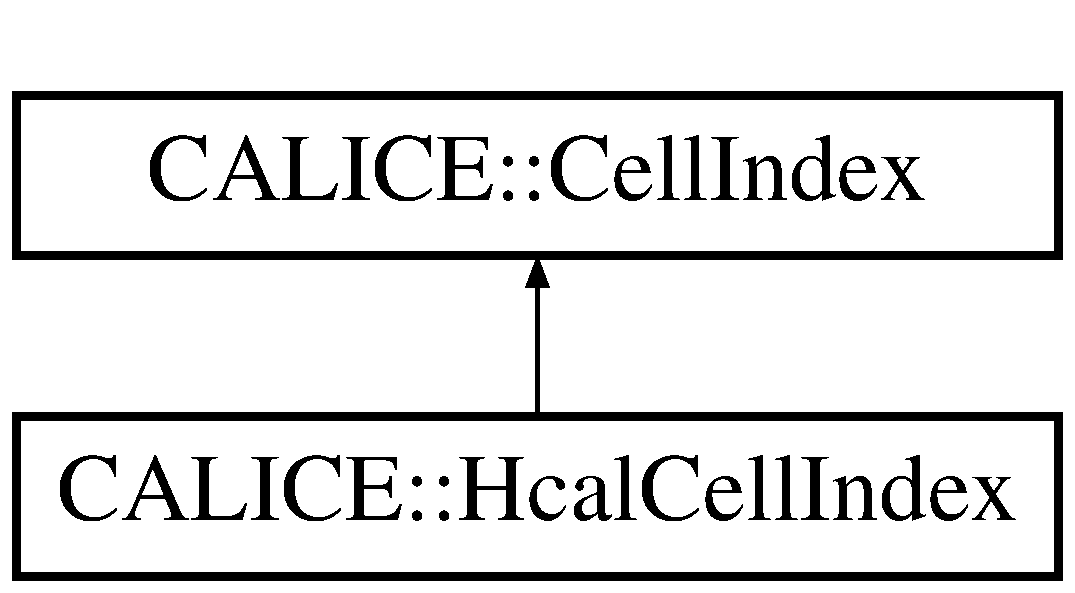
\includegraphics[height=2cm]{classCALICE_1_1CellIndex}
\end{center}
\end{figure}
\subsection*{Public Member Functions}
\begin{DoxyCompactItemize}
\item 
{\bfseries CellIndex} (UInt\_\-t geometrical\_\-cell\_\-index)\label{classCALICE_1_1CellIndex_a4cf7ff45b88a4e2b1062ae7caaa58806}

\item 
{\bfseries CellIndex} (UInt\_\-t geometrical\_\-cell\_\-index, UInt\_\-t second\_\-cell\_\-index)\label{classCALICE_1_1CellIndex_aba275ac1e16f6e6e08ff9b4e4dd61f17}

\item 
{\bfseries CellIndex} (UInt\_\-t wafer\_\-row, UInt\_\-t wafer\_\-column, UInt\_\-t pad\_\-row, UInt\_\-t pad\_\-column, UInt\_\-t layer)\label{classCALICE_1_1CellIndex_a5ab1c3185be6a529aaf2b4476945ac94}

\item 
{\bfseries CellIndex} (UInt\_\-t wafer\_\-row, UInt\_\-t wafer\_\-column, UInt\_\-t pad\_\-row, UInt\_\-t pad\_\-column, UInt\_\-t layer, UInt\_\-t module\_\-index, UInt\_\-t module\_\-type, UInt\_\-t module\_\-ID, UInt\_\-t cell\_\-id, UInt\_\-t isBad)\label{classCALICE_1_1CellIndex_a09201c4195f548a1ecbc740ab5178724}

\item 
{\bfseries CellIndex} (UInt\_\-t geometrical\_\-cell\_\-index, UInt\_\-t module\_\-index, UInt\_\-t module\_\-type, UInt\_\-t module\_\-ID, UInt\_\-t cell\_\-id, UInt\_\-t isBad)\label{classCALICE_1_1CellIndex_a5c849e4daa21098f71c02773466bc2f0}

\item 
UInt\_\-t {\bf getLayerIndex} () const \label{classCALICE_1_1CellIndex_a0467195bc639bda8edba4a9c96e7c0c3}

\begin{DoxyCompactList}\small\item\em Get the layer index (index labeled K in Mokka). \item\end{DoxyCompactList}\item 
{\bf CellIndex} \& {\bf setLayerIndex} (UInt\_\-t layer)\label{classCALICE_1_1CellIndex_a1138c5745d65ec60aa71938eb87bc842}

\begin{DoxyCompactList}\small\item\em Set the layer index (index labeled K in Mokka). \item\end{DoxyCompactList}\item 
UInt\_\-t {\bf getWaferRow} () const \label{classCALICE_1_1CellIndex_a760bda3a8354e9d93d9332220aa7c97d}

\begin{DoxyCompactList}\small\item\em Get the wafer row (index labeled M in Mokka). \item\end{DoxyCompactList}\item 
{\bf CellIndex} \& {\bf setWaferRow} (UInt\_\-t wafer\_\-row)\label{classCALICE_1_1CellIndex_a4a3c7537dd7b4077e5463ae08c4c14f0}

\begin{DoxyCompactList}\small\item\em Set the wafer row (index labeled M in Mokka). \item\end{DoxyCompactList}\item 
UInt\_\-t {\bf getWaferColumn} () const \label{classCALICE_1_1CellIndex_a5b0755196e562f4230eb58aa820b5018}

\begin{DoxyCompactList}\small\item\em Get the wafer column (index labeled S in Mokka). \item\end{DoxyCompactList}\item 
{\bf CellIndex} \& {\bf setWaferColumn} (UInt\_\-t wafer\_\-column)\label{classCALICE_1_1CellIndex_a9680833ddfa0e1137ddc4e4945ecca58}

\begin{DoxyCompactList}\small\item\em Set the wafer column (index labeled S in Mokka). \item\end{DoxyCompactList}\item 
UInt\_\-t {\bf getPadRow} () const \label{classCALICE_1_1CellIndex_aeecbb345a8d7a8215d020ee2ad5a73c3}

\begin{DoxyCompactList}\small\item\em Get the pad row (index labeled J in Mokka). \item\end{DoxyCompactList}\item 
{\bf CellIndex} \& {\bf setPadRow} (UInt\_\-t pad\_\-row)\label{classCALICE_1_1CellIndex_a8e4528b241353e1ae52eb7febecdb371}

\begin{DoxyCompactList}\small\item\em Set the pad row (index labeled J in Mokka). \item\end{DoxyCompactList}\item 
UInt\_\-t {\bf getPadColumn} () const \label{classCALICE_1_1CellIndex_a37471316b7ce32ad1b19f9dc08444193}

\begin{DoxyCompactList}\small\item\em Get the pad column (index labeled I in Mokka). \item\end{DoxyCompactList}\item 
{\bf CellIndex} \& {\bf setPadColumn} (UInt\_\-t pad\_\-column)\label{classCALICE_1_1CellIndex_aa5e1d6c7bf39e5bfbf5ab414405b36d2}

\begin{DoxyCompactList}\small\item\em Set the pad column (index labeled I in Mokka). \item\end{DoxyCompactList}\item 
UInt\_\-t {\bfseries getModuleIndex} () const \label{classCALICE_1_1CellIndex_ad7c3aed04f51baa6a532e2dc18c0b985}

\item 
{\bf CellIndex} \& {\bfseries setModuleIndex} (UInt\_\-t module\_\-index)\label{classCALICE_1_1CellIndex_a87812ed0af0e2c688b21af5a7b3f53fd}

\item 
UInt\_\-t {\bfseries getModuleType} () const \label{classCALICE_1_1CellIndex_ada309da2021a56aa6bb61d0c503f2bd7}

\item 
{\bf CellIndex} \& {\bfseries setModuleType} (UInt\_\-t module\_\-type)\label{classCALICE_1_1CellIndex_aa7541e4208eb9cd7bb5401b324f539e1}

\item 
UInt\_\-t {\bfseries getModuleID} () const \label{classCALICE_1_1CellIndex_a77cabe65a4bd5887963f70eacef6a1b9}

\item 
{\bf CellIndex} \& {\bfseries setModuleID} (UInt\_\-t module\_\-ID)\label{classCALICE_1_1CellIndex_a5cfc410ec22f397a8c21c878e53ab311}

\item 
UInt\_\-t {\bfseries getCellID} () const \label{classCALICE_1_1CellIndex_a8754c16be2ec04e51661f388ff994ebf}

\item 
{\bf CellIndex} \& {\bfseries setCellID} (UInt\_\-t cell\_\-index)\label{classCALICE_1_1CellIndex_a3ecc39a5eb6b4c2d1319d113e1d8b6c3}

\item 
UInt\_\-t {\bfseries isBad} () const \label{classCALICE_1_1CellIndex_a33d6d5bfcc91c6653139a73b5c6ff207}

\item 
{\bf CellIndex} \& {\bfseries setBad} (UInt\_\-t is\_\-bad)\label{classCALICE_1_1CellIndex_aaedafad4a164da776eb9563f6cfecb02}

\item 
UInt\_\-t {\bf getCellIndex} () const \label{classCALICE_1_1CellIndex_a8989a0bfe43f87f5ba5d5f665cc8fd60}

\begin{DoxyCompactList}\small\item\em Get the Mokka conform cell index. \item\end{DoxyCompactList}\item 
{\bf CellIndex} \& {\bf setCellIndex} (UInt\_\-t mokka\_\-cell\_\-index)\label{classCALICE_1_1CellIndex_a06927c6c271b586b2d4f2349ad0a0058}

\begin{DoxyCompactList}\small\item\em Set the Mokka conform cell index. \item\end{DoxyCompactList}\item 
UInt\_\-t {\bf getSecondIndex} () const \label{classCALICE_1_1CellIndex_a62457057612992847f0d1a6791e5eed0}

\begin{DoxyCompactList}\small\item\em Get the 2nd cell index. \item\end{DoxyCompactList}\item 
{\bf CellIndex} \& {\bf setSecondIndex} (UInt\_\-t cellID1)\label{classCALICE_1_1CellIndex_acee8e762e051e2e12e0bfab43be8c441}

\begin{DoxyCompactList}\small\item\em Set the 2nd cell index. \item\end{DoxyCompactList}\end{DoxyCompactItemize}
\subsection*{Private Attributes}
\begin{DoxyCompactItemize}
\item 
UInt\_\-t {\bfseries \_\-index}\label{classCALICE_1_1CellIndex_a0422c3652b611890e2c610eef01fc43e}

\item 
UInt\_\-t {\bfseries \_\-second}\label{classCALICE_1_1CellIndex_adcca7440632d6d8b81aa514a89035b6f}

\end{DoxyCompactItemize}


\subsection{Detailed Description}
The Mokka conform cell index. The cell index encodes the wafer column, and row, pad column and row, and the layer into one index. The wafer 0,0 is in the lower right corner (following a right handed coordinate frame ) looking in beam direction at the detector fron plate. Similar the pad 0,0 of each wafer is located in the lower right corner of the wafer. Encoding for the ECAL: \begin{TabularC}{2}
\hline
M:3,&wafer row \\\cline{1-2}
S-\/1:3,&wafer column \\\cline{1-2}
I:9,&pad coloumn \\\cline{1-2}
J:9,&pad row \\\cline{1-2}
K:6&layer \\\cline{1-2}
\end{TabularC}


Definition at line 102 of file CellIndex.hh.

The documentation for this class was generated from the following file:\begin{DoxyCompactItemize}
\item 
CellIndex.hh\end{DoxyCompactItemize}

\section{CALICE::CellIterator Class Reference}
\label{classCALICE_1_1CellIterator}\index{CALICE::CellIterator@{CALICE::CellIterator}}


iterator to run over all valid (Mokka) cell IDs  


{\ttfamily \#include $<$CellIterator.hh$>$}\subsection*{Public Member Functions}
\begin{DoxyCompactItemize}
\item 
{\bfseries CellIterator} (const {\bf Mapper} $\ast$mapper, const unsigned int index=0)\label{classCALICE_1_1CellIterator_a55f049561c6efd49d8ac05d8fd1892d9}

\item 
void {\bf operator++} ()\label{classCALICE_1_1CellIterator_aa8632dfb854dab0d3afa78eee2d3e4fe}

\begin{DoxyCompactList}\small\item\em jump to the next valid (Mokka) cell ID \item\end{DoxyCompactList}\item 
bool {\bf operator!=} (const {\bf CellIterator} \&other) const \label{classCALICE_1_1CellIterator_afad05336400eeb213d96a7bb837e47da}

\begin{DoxyCompactList}\small\item\em compare if two iterators are not equal \item\end{DoxyCompactList}\item 
bool {\bf operator==} (const {\bf CellIterator} \&other) const \label{classCALICE_1_1CellIterator_a16d97b72ac170520e4ddbcb54ae2b7ae}

\begin{DoxyCompactList}\small\item\em compare if two iterators are equal \item\end{DoxyCompactList}\item 
int {\bf operator$\ast$} () const 
\begin{DoxyCompactList}\small\item\em access to the current (Mokka) cell ID \item\end{DoxyCompactList}\end{DoxyCompactItemize}
\subsection*{Protected Attributes}
\begin{DoxyCompactItemize}
\item 
const {\bf Mapper} $\ast$ {\bfseries \_\-mapper}\label{classCALICE_1_1CellIterator_ac61b53457ed96438d6a3c20658a8b470}

\item 
unsigned int {\bfseries \_\-index}\label{classCALICE_1_1CellIterator_a3ec4eb2ac9ee642f134773d08b382281}

\item 
int {\bfseries \_\-currentCellID}\label{classCALICE_1_1CellIterator_ae8e06dc84e48a482fd2f6ee28d5833eb}

\end{DoxyCompactItemize}


\subsection{Detailed Description}
iterator to run over all valid (Mokka) cell IDs To access the CellID use the $\ast$() operator.

\begin{DoxyAuthor}{Author}
{\tt Benjamin.Lutz@desy.de} 
\end{DoxyAuthor}
\begin{DoxyDate}{Date}
June 2009 
\end{DoxyDate}


Definition at line 18 of file CellIterator.hh.

\subsection{Member Function Documentation}
\index{CALICE::CellIterator@{CALICE::CellIterator}!operator$\ast$@{operator$\ast$}}
\index{operator$\ast$@{operator$\ast$}!CALICE::CellIterator@{CALICE::CellIterator}}
\subsubsection[{operator$\ast$}]{\setlength{\rightskip}{0pt plus 5cm}int CALICE::CellIterator::operator$\ast$ () const\hspace{0.3cm}{\ttfamily  [inline]}}\label{classCALICE_1_1CellIterator_ad5a74f9ea744a9ccac7f40a549ddd4cf}


access to the current (Mokka) cell ID \begin{DoxyReturn}{Returns}
the current cell ID 
\end{DoxyReturn}


Definition at line 43 of file CellIterator.hh.

The documentation for this class was generated from the following files:\begin{DoxyCompactItemize}
\item 
CellIterator.hh\item 
CellIterator.cc\end{DoxyCompactItemize}

\section{CALICE::CellMappingHcal Class Reference}
\label{classCALICE_1_1CellMappingHcal}\index{CALICE::CellMappingHcal@{CALICE::CellMappingHcal}}


Example for a simple mapping class based on the LCFixedObject template.  


{\ttfamily \#include $<$CellMappingHcal.hh$>$}\subsection*{Public Member Functions}
\begin{DoxyCompactItemize}
\item 
{\bf CellMappingHcal} (int icrate, int islot, int ife, int imul, int iadc, int icoord, int jcoord, int kcoord)\label{classCALICE_1_1CellMappingHcal_a180c0b169a7f2c69770ae551aa4c776d}

\begin{DoxyCompactList}\small\item\em Convenient c'tor. \item\end{DoxyCompactList}\item 
{\bf CellMappingHcal} (LCObject $\ast$obj)\label{classCALICE_1_1CellMappingHcal_a0da96ba25246cd5cca90973d362e6c87}

\begin{DoxyCompactList}\small\item\em 'Copy constructor' needed to interpret LCCollection read from file/database. \item\end{DoxyCompactList}\item 
virtual {\bf $\sim$CellMappingHcal} ()\label{classCALICE_1_1CellMappingHcal_a83d82878315eb6feafff6da924cb0b3e}

\begin{DoxyCompactList}\small\item\em Important for memory handling. \item\end{DoxyCompactList}\item 
int {\bf getElecChannel} ()\label{classCALICE_1_1CellMappingHcal_ac7b97417224ddeba13c73d7659484ed0}

\begin{DoxyCompactList}\small\item\em the class interface: \item\end{DoxyCompactList}\item 
int {\bfseries getCellID} ()\label{classCALICE_1_1CellMappingHcal_a5e62c1a1fa22a5d93b59734f5c307fbf}

\item 
short {\bf getCellIndex} (std::string)\label{classCALICE_1_1CellMappingHcal_a4beaa39635a9c718ecbcb98ee336bf4e}

\begin{DoxyCompactList}\small\item\em convenient getter functions \item\end{DoxyCompactList}\item 
short {\bfseries getCrateID} ()\label{classCALICE_1_1CellMappingHcal_a5828458b37828b0bf81007b081bdefdc}

\item 
short {\bfseries getSlotID} ()\label{classCALICE_1_1CellMappingHcal_a83ae95e889acadd9e666421021fc94bd}

\item 
short {\bfseries getFeID} ()\label{classCALICE_1_1CellMappingHcal_a0a0f4e3978887fcb96c2990ad98c7ff8}

\item 
short {\bfseries getMulID} ()\label{classCALICE_1_1CellMappingHcal_ac15468dcd4948f44a67978680748aa54}

\item 
short {\bfseries getAdcID} ()\label{classCALICE_1_1CellMappingHcal_a877867886306a01fe319eab0b00f7256}

\item 
void {\bf print} (std::ostream \&os)\label{classCALICE_1_1CellMappingHcal_a2ffe99f7db6ac95b8e972b37d189f6da}

\begin{DoxyCompactList}\small\item\em Convenient print method. \item\end{DoxyCompactList}\item 
const std::string {\bf getTypeName} () const \label{classCALICE_1_1CellMappingHcal_a03e821c39e5e6452c89954ddcc5038c8}

\begin{DoxyCompactList}\small\item\em Type definition. \item\end{DoxyCompactList}\item 
const std::string {\bf getDataDescription} () const 
\begin{DoxyCompactList}\small\item\em Data description, needed e.g. \item\end{DoxyCompactList}\end{DoxyCompactItemize}
\subsection*{Private Attributes}
\begin{DoxyCompactItemize}
\item 
short {\bf \_\-index}\label{classCALICE_1_1CellMappingHcal_ac042db1cac41c0a080364c6ed8e6e4f5}

\begin{DoxyCompactList}\small\item\em i,j or k Index of the cell id \item\end{DoxyCompactList}\end{DoxyCompactItemize}


\subsection{Detailed Description}
Example for a simple mapping class based on the LCFixedObject template. LCFixedObject uses an instance of LCGenericObjectImpl that holds the data, thus there is no overhead when the data is read from a database or file for copying it to some local structure (Decorator pattern).\par
 

Definition at line 40 of file CellMappingHcal.hh.

\subsection{Member Function Documentation}
\index{CALICE::CellMappingHcal@{CALICE::CellMappingHcal}!getDataDescription@{getDataDescription}}
\index{getDataDescription@{getDataDescription}!CALICE::CellMappingHcal@{CALICE::CellMappingHcal}}
\subsubsection[{getDataDescription}]{\setlength{\rightskip}{0pt plus 5cm}const std::string CALICE::CellMappingHcal::getDataDescription () const\hspace{0.3cm}{\ttfamily  [inline]}}\label{classCALICE_1_1CellMappingHcal_a703c49c4ee36f2faf9ff744afc9bf098}


Data description, needed e.g. by graphical interface to LCCD 

Definition at line 96 of file CellMappingHcal.hh.

The documentation for this class was generated from the following files:\begin{DoxyCompactItemize}
\item 
CellMappingHcal.hh\item 
CellMappingHcal.cc\end{DoxyCompactItemize}

\section{CALICE::CellNeighbourCalculator Class Reference}
\label{classCALICE_1_1CellNeighbourCalculator}\index{CALICE::CellNeighbourCalculator@{CALICE::CellNeighbourCalculator}}


class to calculate all neighbour cells  


{\ttfamily \#include $<$CellNeighbourCalculator.hh$>$}\subsection*{Public Member Functions}
\begin{DoxyCompactItemize}
\item 
{\bf CellNeighbourCalculator} (const {\bf Mapper} $\ast$mapper)
\begin{DoxyCompactList}\small\item\em constructor \item\end{DoxyCompactList}\item 
lcio::LCCollection $\ast$ {\bf getNeighbours} () const 
\begin{DoxyCompactList}\small\item\em get cell neighbours for all valid cells \item\end{DoxyCompactList}\item 
void {\bf getNeighbours} ({\bf MappedContainer}$<$ {\bf CellNeighbours} $>$ $\ast$container) const 
\begin{DoxyCompactList}\small\item\em get cell neighbours for all valid cells \item\end{DoxyCompactList}\end{DoxyCompactItemize}
\subsection*{Protected Member Functions}
\begin{DoxyCompactItemize}
\item 
void {\bfseries checkForCell} (const unsigned int i, const unsigned int j, const unsigned int k, std::set$<$ int $>$ \&cellIDset) const \label{classCALICE_1_1CellNeighbourCalculator_af07fc90a40e8baaf67fac09d53ee2988}

\item 
{\bf CellNeighbours} $\ast$ {\bfseries getNeighbours} (const int cellID) const \label{classCALICE_1_1CellNeighbourCalculator_a687feccba274d8aa4ab40b2c37bf4261}

\end{DoxyCompactItemize}
\subsection*{Private Attributes}
\begin{DoxyCompactItemize}
\item 
const {\bf Mapper} $\ast$ {\bfseries \_\-mapper}\label{classCALICE_1_1CellNeighbourCalculator_a73c7934a2879e61cf0946e5539067181}

\end{DoxyCompactItemize}


\subsection{Detailed Description}
class to calculate all neighbour cells \begin{DoxyAuthor}{Author}
{\tt Benjamin.Lutz@desy.de} 
\end{DoxyAuthor}
\begin{DoxyVersion}{Version}
0.1 
\end{DoxyVersion}
\begin{DoxyDate}{Date}
June 2009 
\end{DoxyDate}


Definition at line 22 of file CellNeighbourCalculator.hh.

\subsection{Constructor \& Destructor Documentation}
\index{CALICE::CellNeighbourCalculator@{CALICE::CellNeighbourCalculator}!CellNeighbourCalculator@{CellNeighbourCalculator}}
\index{CellNeighbourCalculator@{CellNeighbourCalculator}!CALICE::CellNeighbourCalculator@{CALICE::CellNeighbourCalculator}}
\subsubsection[{CellNeighbourCalculator}]{\setlength{\rightskip}{0pt plus 5cm}CALICE::CellNeighbourCalculator::CellNeighbourCalculator (const {\bf Mapper} $\ast$ {\em mapper})}\label{classCALICE_1_1CellNeighbourCalculator_abd2c59c1797a382c0518df7efd9a3108}


constructor 
\begin{DoxyParams}{Parameters}
\item[{\em mapper}]\doxyref{Mapper}{p.}{classCALICE_1_1Mapper} that holds the mapping information from which the neighbours can be generated. \end{DoxyParams}


Definition at line 10 of file CellNeighbourCalculator.cc.

\subsection{Member Function Documentation}
\index{CALICE::CellNeighbourCalculator@{CALICE::CellNeighbourCalculator}!getNeighbours@{getNeighbours}}
\index{getNeighbours@{getNeighbours}!CALICE::CellNeighbourCalculator@{CALICE::CellNeighbourCalculator}}
\subsubsection[{getNeighbours}]{\setlength{\rightskip}{0pt plus 5cm}void CALICE::CellNeighbourCalculator::getNeighbours ({\bf MappedContainer}$<$ {\bf CellNeighbours} $>$ $\ast$ {\em container}) const}\label{classCALICE_1_1CellNeighbourCalculator_ad17cd5438d923800b419794ffa853386}


get cell neighbours for all valid cells 
\begin{DoxyParams}{Parameters}
\item[\mbox{$\rightarrow$} {\em container}]\doxyref{MappedContainer}{p.}{classCALICE_1_1MappedContainer} where the \doxyref{CellNeighbours}{p.}{classCALICE_1_1CellNeighbours} objects should be stored \end{DoxyParams}


Definition at line 103 of file CellNeighbourCalculator.cc.

References CALICE::Mapper::begin(), CALICE::MappedContainer$<$ T $>$::clear(), CALICE::Mapper::end(), CALICE::MappedContainer$<$ T $>$::fillByCellID(), and getNeighbours().\index{CALICE::CellNeighbourCalculator@{CALICE::CellNeighbourCalculator}!getNeighbours@{getNeighbours}}
\index{getNeighbours@{getNeighbours}!CALICE::CellNeighbourCalculator@{CALICE::CellNeighbourCalculator}}
\subsubsection[{getNeighbours}]{\setlength{\rightskip}{0pt plus 5cm}lcio::LCCollection $\ast$ CALICE::CellNeighbourCalculator::getNeighbours () const}\label{classCALICE_1_1CellNeighbourCalculator_a029af1aa53034010a443d205c554e92b}


get cell neighbours for all valid cells \begin{DoxyReturn}{Returns}
LCCollection of \doxyref{CellNeighbours}{p.}{classCALICE_1_1CellNeighbours} objects 
\end{DoxyReturn}


Definition at line 88 of file CellNeighbourCalculator.cc.

References CALICE::Mapper::begin(), and CALICE::Mapper::end().

Referenced by getNeighbours().

The documentation for this class was generated from the following files:\begin{DoxyCompactItemize}
\item 
CellNeighbourCalculator.hh\item 
CellNeighbourCalculator.cc\end{DoxyCompactItemize}

\section{CALICE::CellNeighbours Class Reference}
\label{classCALICE_1_1CellNeighbours}\index{CALICE::CellNeighbours@{CALICE::CellNeighbours}}


class to hold information of neighbouring cells  


{\ttfamily \#include $<$CellNeighbours.hh$>$}\subsection*{Public Types}
\begin{DoxyCompactItemize}
\item 
enum {\bf ENeighbourType} \{ {\bf direct}, 
{\bf corner}, 
{\bfseries k\_\-NneighbourTypes}
 \}
\begin{DoxyCompactList}\small\item\em neighbour type \item\end{DoxyCompactList}\item 
enum {\bf ENeighbourLocation} \{ {\bf module}, 
{\bf forward}, 
{\bf backward}, 
{\bfseries k\_\-NneighbourLocations}
 \}
\begin{DoxyCompactList}\small\item\em neighbour location \item\end{DoxyCompactList}\end{DoxyCompactItemize}
\subsection*{Public Member Functions}
\begin{DoxyCompactItemize}
\item 
{\bf CellNeighbours} (const lcio::LCObject $\ast$obj)
\begin{DoxyCompactList}\small\item\em copy constructor \item\end{DoxyCompactList}\item 
{\bf CellNeighbours} (const lcio::LCGenericObject \&obj)
\begin{DoxyCompactList}\small\item\em copy constructor \item\end{DoxyCompactList}\item 
{\bf CellNeighbours} (const int cellID)
\begin{DoxyCompactList}\small\item\em constructor \item\end{DoxyCompactList}\item 
void {\bf addNeighbour} (const int cellID, const {\bf ENeighbourType} type, const {\bf ENeighbourLocation} location)
\begin{DoxyCompactList}\small\item\em add a neighbour cell \item\end{DoxyCompactList}\item 
int {\bf getCellID} () const 
\begin{DoxyCompactList}\small\item\em get (Mokka) cell ID of master cell \item\end{DoxyCompactList}\item 
const std::vector$<$ int $>$ \& {\bf getNeighbours} (const {\bf ENeighbourType} type, const {\bf ENeighbourLocation} location) const 
\begin{DoxyCompactList}\small\item\em get vector of cell neighbours \item\end{DoxyCompactList}\item 
const std::vector$<$ int $>$ {\bf getNeighbours} (const {\bf ENeighbourType} type) const 
\begin{DoxyCompactList}\small\item\em get vector of cell neighbours \item\end{DoxyCompactList}\item 
const std::vector$<$ int $>$ {\bf getNeighbours} (const {\bf ENeighbourLocation} location) const 
\begin{DoxyCompactList}\small\item\em get vector of cell neighbours \item\end{DoxyCompactList}\item 
const std::vector$<$ int $>$ {\bf getNeighbours} () const 
\begin{DoxyCompactList}\small\item\em get vector of cell neighbours \item\end{DoxyCompactList}\item 
const std::string {\bf getTypeName} () const 
\item 
const std::string {\bf getDataDescription} () const 
\end{DoxyCompactItemize}
\subsection*{Private Types}
\begin{DoxyCompactItemize}
\item 
enum {\bfseries EInt} \{ {\bfseries k\_\-CellID}, 
{\bfseries k\_\-NfixedNumbers}
 \}
\end{DoxyCompactItemize}
\subsection*{Private Member Functions}
\begin{DoxyCompactItemize}
\item 
void {\bfseries copyFromLCGenericObject} (const lcio::LCGenericObject \&obj)\label{classCALICE_1_1CellNeighbours_a399c77122e29b11f0579209c2879a27c}

\item 
void {\bfseries loadValues} ()\label{classCALICE_1_1CellNeighbours_a201d35e317d7483f2ae8807c5dd09ae6}

\item 
void {\bfseries saveValues} ()\label{classCALICE_1_1CellNeighbours_a65f20f02b3553a3a0abb5cf9483f3aee}

\end{DoxyCompactItemize}
\subsection*{Private Attributes}
\begin{DoxyCompactItemize}
\item 
std::ostringstream {\bfseries \_\-dataDescription}\label{classCALICE_1_1CellNeighbours_aaf784e8920b14763e7daedf2b88499dc}

\item 
std::vector$<$ int $>$ {\bfseries \_\-neighbourVectors} [k\_\-NneighbourTypes][k\_\-NneighbourLocations]\label{classCALICE_1_1CellNeighbours_a0f613c9c20d750a3399978eb21263328}

\end{DoxyCompactItemize}
\subsection*{Static Private Attributes}
\begin{DoxyCompactItemize}
\item 
static const std::string {\bfseries neighbourFixedNames} [k\_\-NfixedNumbers] = \{ \char`\"{}cellID\char`\"{} \}\label{classCALICE_1_1CellNeighbours_aee105726874440a5f4c3bfbae89de46b}

\item 
static const std::string {\bfseries neighbourTypeNames} [k\_\-NneighbourTypes]
\item 
static const std::string {\bfseries neighbourLocationNames} [k\_\-NneighbourLocations]
\end{DoxyCompactItemize}


\subsection{Detailed Description}
class to hold information of neighbouring cells \begin{DoxyAuthor}{Author}
{\tt Benjamin.Lutz@desy.de} 
\end{DoxyAuthor}
\begin{DoxyVersion}{Version}
0.1 
\end{DoxyVersion}
\begin{DoxyDate}{Date}
June 2009 
\end{DoxyDate}


Definition at line 21 of file CellNeighbours.hh.

\subsection{Member Enumeration Documentation}
\index{CALICE::CellNeighbours@{CALICE::CellNeighbours}!ENeighbourLocation@{ENeighbourLocation}}
\index{ENeighbourLocation@{ENeighbourLocation}!CALICE::CellNeighbours@{CALICE::CellNeighbours}}
\subsubsection[{ENeighbourLocation}]{\setlength{\rightskip}{0pt plus 5cm}enum {\bf CALICE::CellNeighbours::ENeighbourLocation}}\label{classCALICE_1_1CellNeighbours_affedb8e9d258cd5d11a65c921b92977f}


neighbour location \begin{Desc}
\item[Enumerator: ]\par
\begin{description}
\index{module@{module}!CALICE::CellNeighbours@{CALICE::CellNeighbours}}\index{CALICE::CellNeighbours@{CALICE::CellNeighbours}!module@{module}}\item[{\em 
module\label{classCALICE_1_1CellNeighbours_affedb8e9d258cd5d11a65c921b92977fabb1923c9ce736bd00b553168bce257b1}
}]neighbours within the same module \index{forward@{forward}!CALICE::CellNeighbours@{CALICE::CellNeighbours}}\index{CALICE::CellNeighbours@{CALICE::CellNeighbours}!forward@{forward}}\item[{\em 
forward\label{classCALICE_1_1CellNeighbours_affedb8e9d258cd5d11a65c921b92977fa4e5216e19431a86e213595e2c942a68d}
}]neighbours in the next module (beam direction) \index{backward@{backward}!CALICE::CellNeighbours@{CALICE::CellNeighbours}}\index{CALICE::CellNeighbours@{CALICE::CellNeighbours}!backward@{backward}}\item[{\em 
backward\label{classCALICE_1_1CellNeighbours_affedb8e9d258cd5d11a65c921b92977fa79354e5a35520f80687b76faf7aa62a4}
}]neighbours in the previous module \end{description}
\end{Desc}



Definition at line 44 of file CellNeighbours.hh.\index{CALICE::CellNeighbours@{CALICE::CellNeighbours}!ENeighbourType@{ENeighbourType}}
\index{ENeighbourType@{ENeighbourType}!CALICE::CellNeighbours@{CALICE::CellNeighbours}}
\subsubsection[{ENeighbourType}]{\setlength{\rightskip}{0pt plus 5cm}enum {\bf CALICE::CellNeighbours::ENeighbourType}}\label{classCALICE_1_1CellNeighbours_a89a97dd297d98694875175c22f6c80b9}


neighbour type \begin{Desc}
\item[Enumerator: ]\par
\begin{description}
\index{direct@{direct}!CALICE::CellNeighbours@{CALICE::CellNeighbours}}\index{CALICE::CellNeighbours@{CALICE::CellNeighbours}!direct@{direct}}\item[{\em 
direct\label{classCALICE_1_1CellNeighbours_a89a97dd297d98694875175c22f6c80b9ae61ea93bbf272464e5403ddfbf0a60fc}
}]describes the neighbours that have a common side/surface with the original cell \index{corner@{corner}!CALICE::CellNeighbours@{CALICE::CellNeighbours}}\index{CALICE::CellNeighbours@{CALICE::CellNeighbours}!corner@{corner}}\item[{\em 
corner\label{classCALICE_1_1CellNeighbours_a89a97dd297d98694875175c22f6c80b9a2f63e34121a3a79e0232d0568e51c154}
}]ENeighbourType::corner describes the neighbours that connect to the original cell via a corner \end{description}
\end{Desc}



Definition at line 34 of file CellNeighbours.hh.

\subsection{Constructor \& Destructor Documentation}
\index{CALICE::CellNeighbours@{CALICE::CellNeighbours}!CellNeighbours@{CellNeighbours}}
\index{CellNeighbours@{CellNeighbours}!CALICE::CellNeighbours@{CALICE::CellNeighbours}}
\subsubsection[{CellNeighbours}]{\setlength{\rightskip}{0pt plus 5cm}CALICE::CellNeighbours::CellNeighbours (const lcio::LCObject $\ast$ {\em obj})}\label{classCALICE_1_1CellNeighbours_a190a549359a8902d0d8c5386b23861cd}


copy constructor This constructor is meant to copy-\/convert a \doxyref{CellNeighbours}{p.}{classCALICE_1_1CellNeighbours} object from a LCCollection::getElementAt() call. In contrary to other LCGenericObject derivates, this doesn't reference to the old object, but makes a full copy.


\begin{DoxyParams}{Parameters}
\item[\mbox{$\leftarrow$} {\em obj}]LCObject pointer to a \doxyref{CellNeighbours}{p.}{classCALICE_1_1CellNeighbours} object \end{DoxyParams}


Definition at line 15 of file CellNeighbours.cc.\index{CALICE::CellNeighbours@{CALICE::CellNeighbours}!CellNeighbours@{CellNeighbours}}
\index{CellNeighbours@{CellNeighbours}!CALICE::CellNeighbours@{CALICE::CellNeighbours}}
\subsubsection[{CellNeighbours}]{\setlength{\rightskip}{0pt plus 5cm}CALICE::CellNeighbours::CellNeighbours (const lcio::LCGenericObject \& {\em obj})}\label{classCALICE_1_1CellNeighbours_a34ce6eed0846685f8b32342f5249820f}


copy constructor This constructor is meant to copy-\/convert a \doxyref{CellNeighbours}{p.}{classCALICE_1_1CellNeighbours} object from a LCGenericObject.


\begin{DoxyParams}{Parameters}
\item[\mbox{$\leftarrow$} {\em obj}]LCGenericObject of type \doxyref{CellNeighbours}{p.}{classCALICE_1_1CellNeighbours} which should be copied \end{DoxyParams}


Definition at line 25 of file CellNeighbours.cc.\index{CALICE::CellNeighbours@{CALICE::CellNeighbours}!CellNeighbours@{CellNeighbours}}
\index{CellNeighbours@{CellNeighbours}!CALICE::CellNeighbours@{CALICE::CellNeighbours}}
\subsubsection[{CellNeighbours}]{\setlength{\rightskip}{0pt plus 5cm}CALICE::CellNeighbours::CellNeighbours (const int {\em cellID})}\label{classCALICE_1_1CellNeighbours_ad6d1861dd68ea60d4b3020fd8b623c49}


constructor 
\begin{DoxyParams}{Parameters}
\item[\mbox{$\leftarrow$} {\em cellID}](Mokka) cell ID of the master cell \end{DoxyParams}


Definition at line 44 of file CellNeighbours.cc.

\subsection{Member Function Documentation}
\index{CALICE::CellNeighbours@{CALICE::CellNeighbours}!addNeighbour@{addNeighbour}}
\index{addNeighbour@{addNeighbour}!CALICE::CellNeighbours@{CALICE::CellNeighbours}}
\subsubsection[{addNeighbour}]{\setlength{\rightskip}{0pt plus 5cm}void CALICE::CellNeighbours::addNeighbour (const int {\em cellID}, \/  const {\bf ENeighbourType} {\em type}, \/  const {\bf ENeighbourLocation} {\em location})}\label{classCALICE_1_1CellNeighbours_ab67f7a002e853e749d4f376f423728e6}


add a neighbour cell 
\begin{DoxyParams}{Parameters}
\item[\mbox{$\leftarrow$} {\em cellID}](Mokka) cell ID of the neighbour cell \item[\mbox{$\leftarrow$} {\em type}]cell neighbour type \item[\mbox{$\leftarrow$} {\em location}]cell neighbour location\end{DoxyParams}
\begin{DoxySeeAlso}{See also}
\doxyref{ENeighbourType}{p.}{classCALICE_1_1CellNeighbours_a89a97dd297d98694875175c22f6c80b9} 

\doxyref{ENeighbourLocation}{p.}{classCALICE_1_1CellNeighbours_affedb8e9d258cd5d11a65c921b92977f} 
\end{DoxySeeAlso}


Definition at line 48 of file CellNeighbours.cc.\index{CALICE::CellNeighbours@{CALICE::CellNeighbours}!getCellID@{getCellID}}
\index{getCellID@{getCellID}!CALICE::CellNeighbours@{CALICE::CellNeighbours}}
\subsubsection[{getCellID}]{\setlength{\rightskip}{0pt plus 5cm}int CALICE::CellNeighbours::getCellID () const}\label{classCALICE_1_1CellNeighbours_a33159faedeb9914b99aa34b9475ecc3e}


get (Mokka) cell ID of master cell \begin{DoxyReturn}{Returns}
(Mokka) cell ID of master cell 
\end{DoxyReturn}


Definition at line 53 of file CellNeighbours.cc.\index{CALICE::CellNeighbours@{CALICE::CellNeighbours}!getDataDescription@{getDataDescription}}
\index{getDataDescription@{getDataDescription}!CALICE::CellNeighbours@{CALICE::CellNeighbours}}
\subsubsection[{getDataDescription}]{\setlength{\rightskip}{0pt plus 5cm}const std::string CALICE::CellNeighbours::getDataDescription () const\hspace{0.3cm}{\ttfamily  [inline]}}\label{classCALICE_1_1CellNeighbours_a60088866e16cca8e21a193a2f49b43c1}
\begin{DoxyReturn}{Returns}
LCGenericObject data description 
\end{DoxyReturn}


Definition at line 141 of file CellNeighbours.hh.\index{CALICE::CellNeighbours@{CALICE::CellNeighbours}!getNeighbours@{getNeighbours}}
\index{getNeighbours@{getNeighbours}!CALICE::CellNeighbours@{CALICE::CellNeighbours}}
\subsubsection[{getNeighbours}]{\setlength{\rightskip}{0pt plus 5cm}const std::vector$<$ int $>$ CALICE::CellNeighbours::getNeighbours () const}\label{classCALICE_1_1CellNeighbours_a4c73949c6faeccabc206522d86037180}


get vector of cell neighbours \begin{DoxyReturn}{Returns}
vector with (Mokka) cell IDs from all neighbours 
\end{DoxyReturn}


Definition at line 61 of file CellNeighbours.cc.\index{CALICE::CellNeighbours@{CALICE::CellNeighbours}!getNeighbours@{getNeighbours}}
\index{getNeighbours@{getNeighbours}!CALICE::CellNeighbours@{CALICE::CellNeighbours}}
\subsubsection[{getNeighbours}]{\setlength{\rightskip}{0pt plus 5cm}const std::vector$<$ int $>$ CALICE::CellNeighbours::getNeighbours (const {\bf ENeighbourLocation} {\em location}) const}\label{classCALICE_1_1CellNeighbours_a6a17a783fdfd9ad8e758dcd78a2ad262}


get vector of cell neighbours 
\begin{DoxyParams}{Parameters}
\item[\mbox{$\leftarrow$} {\em location}]location of the neighbours requested\end{DoxyParams}
\begin{DoxyReturn}{Returns}
vector with (Mokka) cell IDs from the neighbours of the requested location 
\end{DoxyReturn}


Definition at line 82 of file CellNeighbours.cc.\index{CALICE::CellNeighbours@{CALICE::CellNeighbours}!getNeighbours@{getNeighbours}}
\index{getNeighbours@{getNeighbours}!CALICE::CellNeighbours@{CALICE::CellNeighbours}}
\subsubsection[{getNeighbours}]{\setlength{\rightskip}{0pt plus 5cm}const std::vector$<$ int $>$ CALICE::CellNeighbours::getNeighbours (const {\bf ENeighbourType} {\em type}) const}\label{classCALICE_1_1CellNeighbours_a95ed1e7949c32398354fc8885d7f642c}


get vector of cell neighbours 
\begin{DoxyParams}{Parameters}
\item[\mbox{$\leftarrow$} {\em type}]type of the neighbours requested\end{DoxyParams}
\begin{DoxyReturn}{Returns}
vector with (Mokka) cell IDs from the neighbours of the requested type 
\end{DoxyReturn}


Definition at line 72 of file CellNeighbours.cc.\index{CALICE::CellNeighbours@{CALICE::CellNeighbours}!getNeighbours@{getNeighbours}}
\index{getNeighbours@{getNeighbours}!CALICE::CellNeighbours@{CALICE::CellNeighbours}}
\subsubsection[{getNeighbours}]{\setlength{\rightskip}{0pt plus 5cm}const std::vector$<$ int $>$ \& CALICE::CellNeighbours::getNeighbours (const {\bf ENeighbourType} {\em type}, \/  const {\bf ENeighbourLocation} {\em location}) const}\label{classCALICE_1_1CellNeighbours_ae25db0074d4bc41acf76cd01e9df08db}


get vector of cell neighbours This function is more efficient as the other getNeighbours function, as a const reference to the internal data is returned and no copying of elements is necessary.


\begin{DoxyParams}{Parameters}
\item[\mbox{$\leftarrow$} {\em type}]type of the neighbours requested \item[\mbox{$\leftarrow$} {\em location}]location of the neighbours requested\end{DoxyParams}
\begin{DoxyReturn}{Returns}
vector with (Mokka) cell IDs from the neighbours of the requested type and location 
\end{DoxyReturn}


Definition at line 57 of file CellNeighbours.cc.\index{CALICE::CellNeighbours@{CALICE::CellNeighbours}!getTypeName@{getTypeName}}
\index{getTypeName@{getTypeName}!CALICE::CellNeighbours@{CALICE::CellNeighbours}}
\subsubsection[{getTypeName}]{\setlength{\rightskip}{0pt plus 5cm}const std::string CALICE::CellNeighbours::getTypeName () const\hspace{0.3cm}{\ttfamily  [inline]}}\label{classCALICE_1_1CellNeighbours_a9bf6a7e74b1e8f98153ca3dce59523b7}
\begin{DoxyReturn}{Returns}
LCGenericObject data type name 
\end{DoxyReturn}


Definition at line 137 of file CellNeighbours.hh.

\subsection{Field Documentation}
\index{CALICE::CellNeighbours@{CALICE::CellNeighbours}!neighbourLocationNames@{neighbourLocationNames}}
\index{neighbourLocationNames@{neighbourLocationNames}!CALICE::CellNeighbours@{CALICE::CellNeighbours}}
\subsubsection[{neighbourLocationNames}]{\setlength{\rightskip}{0pt plus 5cm}const std::string CALICE::CellNeighbours::neighbourLocationNames\hspace{0.3cm}{\ttfamily  [static, private]}}\label{classCALICE_1_1CellNeighbours_a064d2b1a737839e76c6ca0d33320be72}
{\bfseries Initial value:}
\begin{DoxyCode}
 { "module",
                                                                                 
                           "forward",
                                                                                 
                           "backward"}
\end{DoxyCode}


Definition at line 50 of file CellNeighbours.hh.\index{CALICE::CellNeighbours@{CALICE::CellNeighbours}!neighbourTypeNames@{neighbourTypeNames}}
\index{neighbourTypeNames@{neighbourTypeNames}!CALICE::CellNeighbours@{CALICE::CellNeighbours}}
\subsubsection[{neighbourTypeNames}]{\setlength{\rightskip}{0pt plus 5cm}const std::string CALICE::CellNeighbours::neighbourTypeNames\hspace{0.3cm}{\ttfamily  [static, private]}}\label{classCALICE_1_1CellNeighbours_a2eedc7bbb8e228cae9884b776d6761f0}
{\bfseries Initial value:}
\begin{DoxyCode}
 { "direct",
                                                                                 
                   "corner" }
\end{DoxyCode}


Definition at line 49 of file CellNeighbours.hh.

The documentation for this class was generated from the following files:\begin{DoxyCompactItemize}
\item 
CellNeighbours.hh\item 
CellNeighbours.cc\end{DoxyCompactItemize}

\section{CALICE::CellQuality Class Reference}
\label{classCALICE_1_1CellQuality}\index{CALICE::CellQuality@{CALICE::CellQuality}}


LCIO contions data class to describe the cell quality.  


{\ttfamily \#include $<$CellQuality.hh$>$}\subsection*{Public Member Functions}
\begin{DoxyCompactItemize}
\item 
{\bf CellQuality} (const int id, const int status=0)
\begin{DoxyCompactList}\small\item\em Initialise the \doxyref{CellQuality}{p.}{classCALICE_1_1CellQuality} with the CellID. \item\end{DoxyCompactList}\item 
{\bfseries CellQuality} (EVENT::LCObject $\ast$)\label{classCALICE_1_1CellQuality_a67a0a10871b506705a93d15c5c9f1398}

\item 
const int {\bf getCellID} () const \label{classCALICE_1_1CellQuality_a5c4b83d65a3e51683c7f1de9609c9cd8}

\begin{DoxyCompactList}\small\item\em Get the cell ID. \item\end{DoxyCompactList}\item 
const int {\bf getStatus} () const \label{classCALICE_1_1CellQuality_a1ec6dbf56828da5575e9d268632d534d}

\begin{DoxyCompactList}\small\item\em Get the status. \item\end{DoxyCompactList}\item 
bool {\bf isDead} () const \label{classCALICE_1_1CellQuality_ad886e21dfeb1e49da166a72f5394baa5}

\begin{DoxyCompactList}\small\item\em Check if the cell has been marked as dead. \item\end{DoxyCompactList}\item 
bool {\bf isNoisy} () const \label{classCALICE_1_1CellQuality_a7c90423f24c3c29bb8b1d7ab2d612f02}

\begin{DoxyCompactList}\small\item\em Check if the cell has been marked as noisy. \item\end{DoxyCompactList}\item 
void {\bf setDead} (bool dead=true)\label{classCALICE_1_1CellQuality_a009ab8aa42248bfad012b8583dad272a}

\begin{DoxyCompactList}\small\item\em Set the dead flag. By using {\ttfamily setDead(false)} you can unset the dead status. \item\end{DoxyCompactList}\item 
void {\bf setNoisy} (bool noisy=true)\label{classCALICE_1_1CellQuality_a116fcb57a8e8c0de606b30c62fb3a46c}

\begin{DoxyCompactList}\small\item\em Set the noisy flag. By using {\ttfamily setNoisy(false)} you can unset the noisy status. \item\end{DoxyCompactList}\item 
virtual const std::string {\bfseries getTypeName} () const \label{classCALICE_1_1CellQuality_a016d2d5250c6bdb0163f65e346e0aa38}

\item 
virtual const std::string {\bfseries getDataDescription} () const \label{classCALICE_1_1CellQuality_ade0507fb47735c097963655f99ec87eb}

\end{DoxyCompactItemize}
\subsection*{Static Protected Attributes}
\begin{DoxyCompactItemize}
\item 
static const int {\bf \_\-dead} = 0x1\label{classCALICE_1_1CellQuality_a678fd1b8a9b414839b46336c345d642c}

\begin{DoxyCompactList}\small\item\em the dead bit: 0x1 \item\end{DoxyCompactList}\item 
static const int {\bf \_\-noisy} = 0x2\label{classCALICE_1_1CellQuality_a46bbb8d66e2ac749976f7a4bffbe4df6}

\begin{DoxyCompactList}\small\item\em the noisy bit: 0x2 \item\end{DoxyCompactList}\end{DoxyCompactItemize}
\subsection*{Private Member Functions}
\begin{DoxyCompactItemize}
\item 
void {\bf setStatus} (int status)
\begin{DoxyCompactList}\small\item\em The setting of the status is private. \item\end{DoxyCompactList}\end{DoxyCompactItemize}


\subsection{Detailed Description}
LCIO contions data class to describe the cell quality. The cell can be dead or noisy (or both, for instance if a cell is noisy and then dies during a run period).

Note: Internally the status is treated as a bit pattern, which allows setting several flags simulaneously and can easily be extended. Thanks to the user interface the user never has to fiddle around with the bits. The definition is protected inside the class and queried with \doxyref{isDead()}{p.}{classCALICE_1_1CellQuality_ad886e21dfeb1e49da166a72f5394baa5} or \doxyref{isNoisy()}{p.}{classCALICE_1_1CellQuality_a7c90423f24c3c29bb8b1d7ab2d612f02}.

\begin{DoxyAuthor}{Author}
Niels Meyer, Desy 

Martin Killenberg, CERN 
\end{DoxyAuthor}


Definition at line 23 of file CellQuality.hh.

\subsection{Constructor \& Destructor Documentation}
\index{CALICE::CellQuality@{CALICE::CellQuality}!CellQuality@{CellQuality}}
\index{CellQuality@{CellQuality}!CALICE::CellQuality@{CALICE::CellQuality}}
\subsubsection[{CellQuality}]{\setlength{\rightskip}{0pt plus 5cm}CALICE::CellQuality::CellQuality (const int {\em id}, \/  const int {\em status} = {\ttfamily 0})}\label{classCALICE_1_1CellQuality_adcbec5052d671a6784ea785bb1521d79}


Initialise the \doxyref{CellQuality}{p.}{classCALICE_1_1CellQuality} with the CellID. When the status is already know it can also be given to the constructor (optional). 

Definition at line 11 of file CellQuality.cc.

References setStatus().

\subsection{Member Function Documentation}
\index{CALICE::CellQuality@{CALICE::CellQuality}!setStatus@{setStatus}}
\index{setStatus@{setStatus}!CALICE::CellQuality@{CALICE::CellQuality}}
\subsubsection[{setStatus}]{\setlength{\rightskip}{0pt plus 5cm}void CALICE::CellQuality::setStatus (int {\em status})\hspace{0.3cm}{\ttfamily  [private]}}\label{classCALICE_1_1CellQuality_a96b044851c3c6c3d7526291ad005a6bf}


The setting of the status is private. It is only allowed using the conctructor or the set() functions. 

Definition at line 19 of file CellQuality.cc.

Referenced by CellQuality(), setDead(), and setNoisy().

The documentation for this class was generated from the following files:\begin{DoxyCompactItemize}
\item 
CellQuality.hh\item 
CellQuality.cc\end{DoxyCompactItemize}

\section{CALICE::ClusterShapesTyped Class Reference}
\label{classCALICE_1_1ClusterShapesTyped}\index{CALICE::ClusterShapesTyped@{CALICE::ClusterShapesTyped}}
\subsection*{Public Member Functions}
\begin{DoxyCompactItemize}
\item 
{\footnotesize template$<$class T $>$ }\\void {\bfseries fill} (const lcio::LCCollection $\ast$col)\label{classCALICE_1_1ClusterShapesTyped_afb62e9b658c7420051df7d997aa02800}

\item 
ClusterShapes $\ast$ {\bfseries getClusterShapesPointer} ()\label{classCALICE_1_1ClusterShapesTyped_a856df7a286fb0facfd9a87ae11286ec9}

\item 
ClusterShapes $\ast$$\ast$ {\bfseries getClusterShapesPointerPointer} ()\label{classCALICE_1_1ClusterShapesTyped_a9d3fabcc3aebb217c7c5673c077bb4ea}

\end{DoxyCompactItemize}
\subsection*{Private Member Functions}
\begin{DoxyCompactItemize}
\item 
void {\bfseries generateShapes} ()\label{classCALICE_1_1ClusterShapesTyped_a0526e8ad7d133ee4b3fee30d13f72d66}

\end{DoxyCompactItemize}
\subsection*{Private Attributes}
\begin{DoxyCompactItemize}
\item 
ClusterShapes $\ast$ {\bfseries \_\-shapes}\label{classCALICE_1_1ClusterShapesTyped_abefd2921e7b46295049038249a341e0c}

\item 
ClusterShapes $\ast$$\ast$ {\bfseries \_\-shapesPointer}\label{classCALICE_1_1ClusterShapesTyped_ab876f0147f6c5637461214d6373ba5ab}

\item 
std::vector$<$ float $>$ {\bfseries \_\-aHit}\label{classCALICE_1_1ClusterShapesTyped_aa04563ae806937cc66e2ea67c7793449}

\item 
std::vector$<$ float $>$ {\bfseries \_\-xHit}\label{classCALICE_1_1ClusterShapesTyped_a4392fd32a786c63115624cb82218c509}

\item 
std::vector$<$ float $>$ {\bfseries \_\-yHit}\label{classCALICE_1_1ClusterShapesTyped_ac7e0b672703cd19d2327a774d2472bf7}

\item 
std::vector$<$ float $>$ {\bfseries \_\-zHit}\label{classCALICE_1_1ClusterShapesTyped_acd58104f72c22a4d34b3455c17fc361c}

\end{DoxyCompactItemize}


\subsection{Detailed Description}


Definition at line 10 of file ClusterShapesTyped.hh.

The documentation for this class was generated from the following file:\begin{DoxyCompactItemize}
\item 
ClusterShapesTyped.hh\end{DoxyCompactItemize}

\section{CALICE::ConditionsChangeDelegator$<$ T $>$ Class Template Reference}
\label{classCALICE_1_1ConditionsChangeDelegator}\index{CALICE::ConditionsChangeDelegator@{CALICE::ConditionsChangeDelegator}}


Listens for conditions data changes and delegates the information to a class.  


{\ttfamily \#include $<$ConditionsChangeDelegator.hh$>$}\subsection*{Public Types}
\begin{DoxyCompactItemize}
\item 
typedef void(T::$\ast$ {\bfseries ConditionsChangeHandleFunc\_\-t} )(lcio::LCCollection $\ast$col)\label{classCALICE_1_1ConditionsChangeDelegator_afd68318ab8917fd1f97d18ae8204c167}

\end{DoxyCompactItemize}
\subsection*{Public Member Functions}
\begin{DoxyCompactItemize}
\item 
{\bfseries ConditionsChangeDelegator} (T $\ast$responsible, ConditionsChangeHandleFunc\_\-t a\_\-func)\label{classCALICE_1_1ConditionsChangeDelegator_a724d008ad96b77fa64b8716545052b57}

\item 
void {\bf conditionsChanged} (lcio::LCCollection $\ast$col)
\begin{DoxyCompactList}\small\item\em Be notified if conditions data changes and redirect changes to responsible class. \item\end{DoxyCompactList}\end{DoxyCompactItemize}
\subsection*{Private Attributes}
\begin{DoxyCompactItemize}
\item 
ConditionsChangeHandleFunc\_\-t {\bf \_\-funcP}\label{classCALICE_1_1ConditionsChangeDelegator_adaf17b9ce91ac651de46c007b69f5719}

\begin{DoxyCompactList}\small\item\em method to be called if the conditions data changed \item\end{DoxyCompactList}\item 
T $\ast$ {\bf \_\-responsible}\label{classCALICE_1_1ConditionsChangeDelegator_a0d8f29b22856a229930ee6246ad066fd}

\begin{DoxyCompactList}\small\item\em the object which will take care of the change \item\end{DoxyCompactList}\end{DoxyCompactItemize}


\subsection{Detailed Description}
\subsubsection*{template$<$class T$>$ class CALICE::ConditionsChangeDelegator$<$ T $>$}

Listens for conditions data changes and delegates the information to a class. a class can redirect several conditions data changes to itself. \begin{DoxySeeAlso}{See also}
testConditionsDataDelegator.cc 
\end{DoxySeeAlso}


Definition at line 13 of file ConditionsChangeDelegator.hh.

\subsection{Member Function Documentation}
\index{CALICE::ConditionsChangeDelegator@{CALICE::ConditionsChangeDelegator}!conditionsChanged@{conditionsChanged}}
\index{conditionsChanged@{conditionsChanged}!CALICE::ConditionsChangeDelegator@{CALICE::ConditionsChangeDelegator}}
\subsubsection[{conditionsChanged}]{\setlength{\rightskip}{0pt plus 5cm}template$<$class T$>$ void {\bf CALICE::ConditionsChangeDelegator}$<$ T $>$::conditionsChanged (lcio::LCCollection $\ast$ {\em col})\hspace{0.3cm}{\ttfamily  [inline]}}\label{classCALICE_1_1ConditionsChangeDelegator_a4eae95674a704dd8d59a6fb4ca1490ea}


Be notified if conditions data changes and redirect changes to responsible class. 
\begin{DoxyParams}{Parameters}
\item[{\em col}]the collection containing the new conditions data \end{DoxyParams}


Definition at line 26 of file ConditionsChangeDelegator.hh.

The documentation for this class was generated from the following file:\begin{DoxyCompactItemize}
\item 
ConditionsChangeDelegator.hh\end{DoxyCompactItemize}

\section{CALICE::ConditionsDataWriteHandler Class Reference}
\label{classCALICE_1_1ConditionsDataWriteHandler}\index{CALICE::ConditionsDataWriteHandler@{CALICE::ConditionsDataWriteHandler}}


Handler of conditions data changes which writes the replaced collections to a conditions data base.  


{\ttfamily \#include $<$ConditionsDataWriteHandler.hh$>$}\subsection*{Public Member Functions}
\begin{DoxyCompactItemize}
\item 
{\bf ConditionsDataWriteHandler} (const std::string \&col\_\-name, const std::string \&db\_\-init\_\-string, const std::string \&folder\_\-name, const std::string \&tag, const std::string \&description)
\begin{DoxyCompactList}\small\item\em constructor. \item\end{DoxyCompactList}\item 
{\bf $\sim$ConditionsDataWriteHandler} ()\label{classCALICE_1_1ConditionsDataWriteHandler_a581dea40c8faa28948c8cb461d9126dc}

\begin{DoxyCompactList}\small\item\em destructor. \item\end{DoxyCompactList}\item 
void {\bf conditionsChanged} (lcio::LCCollection $\ast$col)
\begin{DoxyCompactList}\small\item\em Be notified if conditions data changes and redirect changes to responsible class. \item\end{DoxyCompactList}\item 
void {\bf writeConditionsData} (const long64 \&best\_\-guess\_\-of\_\-till\_\-time\_\-stamp)
\begin{DoxyCompactList}\small\item\em write the conditions data to the conditions database. \item\end{DoxyCompactList}\item 
void {\bf setSinceTime} (long64 since\_\-time)
\begin{DoxyCompactList}\small\item\em Set the correct since time for the current conditions data. \item\end{DoxyCompactList}\item 
const std::string \& {\bfseries name} () const \label{classCALICE_1_1ConditionsDataWriteHandler_a578e53e8c53ee791d1ab574811551496}

\item 
unsigned int {\bf numberOfWrites} () const \label{classCALICE_1_1ConditionsDataWriteHandler_a535ca783c3475b0cbacd99484c4e4229}

\begin{DoxyCompactList}\small\item\em Get the number of collections written to the database;. \item\end{DoxyCompactList}\item 
unsigned int {\bf changes} () const \label{classCALICE_1_1ConditionsDataWriteHandler_ae53d14eec368dc28b8bc5dcb73ed2d01}

\begin{DoxyCompactList}\small\item\em Get the number of recognised changes of the conditions data. \item\end{DoxyCompactList}\item 
long64 {\bf validAtMostSince} () const \label{classCALICE_1_1ConditionsDataWriteHandler_a1899ab4669280acec16c6baa53e6abc3}

\begin{DoxyCompactList}\small\item\em Get the time of the first recognised conditions data change. \item\end{DoxyCompactList}\item 
long64 {\bf validAtMostTill} () const \label{classCALICE_1_1ConditionsDataWriteHandler_a487fe71c6d796b46dac6dd7ea16eb917}

\begin{DoxyCompactList}\small\item\em Get the time of the last write to the data base. \item\end{DoxyCompactList}\item 
long64 {\bf currentValidSince} () const \label{classCALICE_1_1ConditionsDataWriteHandler_ac3a420cb581ed9519e06e795dd13ac9a}

\begin{DoxyCompactList}\small\item\em Get the time of the first recognised conditions data change. \item\end{DoxyCompactList}\item 
long64 {\bf currentValidTill} () const \label{classCALICE_1_1ConditionsDataWriteHandler_a7cae6dc5fd78a5aa243bb589ba4c7caa}

\begin{DoxyCompactList}\small\item\em Get the time of the last write to the data base. \item\end{DoxyCompactList}\item 
const std::string \& {\bfseries getTag} () const \label{classCALICE_1_1ConditionsDataWriteHandler_a3e14961a4bf03b6282f2b59fe87790fa}

\end{DoxyCompactItemize}
\subsection*{Private Attributes}
\begin{DoxyCompactItemize}
\item 
const std::string {\bf \_\-colName}\label{classCALICE_1_1ConditionsDataWriteHandler_a7e065bb6ab09b579ce20f7dbbbdf07a2}

\begin{DoxyCompactList}\small\item\em name of the collection (not used) \item\end{DoxyCompactList}\item 
lccd::DBInterface {\bfseries \_\-db}\label{classCALICE_1_1ConditionsDataWriteHandler_a94ae745611b1bff4441eab7677c408c1}

\item 
lccd::IConditionsHandler $\ast$ {\bf \_\-changeHandler}\label{classCALICE_1_1ConditionsDataWriteHandler_a3a20bce4a053386c2d4f786653438f38}

\begin{DoxyCompactList}\small\item\em handler of the conditions data \item\end{DoxyCompactList}\item 
const std::string {\bfseries \_\-tag}\label{classCALICE_1_1ConditionsDataWriteHandler_a62de4dca742011f4fdb976d4bb3abee2}

\item 
const std::string {\bfseries \_\-description}\label{classCALICE_1_1ConditionsDataWriteHandler_a01342556e5b2c4916dbb3d3705dd0af3}

\item 
long64 {\bf \_\-since}
\begin{DoxyCompactList}\small\item\em the time of the event just before the conditions data changed. \item\end{DoxyCompactList}\item 
long64 {\bf \_\-till}
\begin{DoxyCompactList}\small\item\em Best guess of the till time stamp (may be wrong). \item\end{DoxyCompactList}\item 
LCCollection $\ast$ {\bf \_\-col}
\begin{DoxyCompactList}\small\item\em pointer to the clone of the conditions data collection. \item\end{DoxyCompactList}\item 
unsigned int {\bf \_\-changes}
\begin{DoxyCompactList}\small\item\em keep track of the number of changes. \item\end{DoxyCompactList}\item 
unsigned int {\bf \_\-writes}
\begin{DoxyCompactList}\small\item\em keep track of the number of conditions data written to the database. \item\end{DoxyCompactList}\item 
long64 {\bfseries \_\-first}\label{classCALICE_1_1ConditionsDataWriteHandler_a8076fe1b19e269527fa769de5a88a65e}

\item 
long64 {\bfseries \_\-last}\label{classCALICE_1_1ConditionsDataWriteHandler_a5debaace61a41f99d2df0ce318c036bf}

\end{DoxyCompactItemize}


\subsection{Detailed Description}
Handler of conditions data changes which writes the replaced collections to a conditions data base. When ever conditions data changes the old (cloned) collection will be stored with the time stamps of the event just before the former conditions data change and the time stamp of the last event. At the end of the run, the conditions data has to be written manually by calling \doxyref{writeConditionsData()}{p.}{classCALICE_1_1ConditionsDataWriteHandler_a139623a650f56c24a5d32658da9af09b} with the time stamp of the last event. 

Definition at line 40 of file ConditionsDataWriteHandler.hh.

\subsection{Constructor \& Destructor Documentation}
\index{CALICE::ConditionsDataWriteHandler@{CALICE::ConditionsDataWriteHandler}!ConditionsDataWriteHandler@{ConditionsDataWriteHandler}}
\index{ConditionsDataWriteHandler@{ConditionsDataWriteHandler}!CALICE::ConditionsDataWriteHandler@{CALICE::ConditionsDataWriteHandler}}
\subsubsection[{ConditionsDataWriteHandler}]{\setlength{\rightskip}{0pt plus 5cm}CALICE::ConditionsDataWriteHandler::ConditionsDataWriteHandler (const std::string \& {\em col\_\-name}, \/  const std::string \& {\em db\_\-init\_\-string}, \/  const std::string \& {\em folder\_\-name}, \/  const std::string \& {\em tag}, \/  const std::string \& {\em description})}\label{classCALICE_1_1ConditionsDataWriteHandler_ae0e0b43ca010d9a424f962480175b110}


constructor. 
\begin{DoxyParams}{Parameters}
\item[{\em col\_\-name}]the name of the to be monitored collection (not needed). \item[{\em db\_\-init\_\-string}]specifier of the database host name, database name, user and password. \item[{\em folder\_\-name}]name of the destination folder. \item[{\em tag}]to be applied at the end of the run to the folder. \item[{\em description}]the description added to every collection written toe the data base. \end{DoxyParams}


Definition at line 15 of file ConditionsDataWriteHandler.cc.

References \_\-changeHandler, \_\-colName, \_\-since, and \_\-till.

\subsection{Member Function Documentation}
\index{CALICE::ConditionsDataWriteHandler@{CALICE::ConditionsDataWriteHandler}!conditionsChanged@{conditionsChanged}}
\index{conditionsChanged@{conditionsChanged}!CALICE::ConditionsDataWriteHandler@{CALICE::ConditionsDataWriteHandler}}
\subsubsection[{conditionsChanged}]{\setlength{\rightskip}{0pt plus 5cm}void CALICE::ConditionsDataWriteHandler::conditionsChanged (lcio::LCCollection $\ast$ {\em col})}\label{classCALICE_1_1ConditionsDataWriteHandler_a0289e54f162d87125bce02b71dc46b51}


Be notified if conditions data changes and redirect changes to responsible class. 
\begin{DoxyParams}{Parameters}
\item[{\em col}]the collection containing the new conditions data \end{DoxyParams}


if (\_\-changeHandler) \{ 

Definition at line 59 of file ConditionsDataWriteHandler.cc.

References \_\-changeHandler, \_\-changes, \_\-col, \_\-colName, \_\-since, \_\-till, CALICE::cloneCollection(), and writeConditionsData().\index{CALICE::ConditionsDataWriteHandler@{CALICE::ConditionsDataWriteHandler}!setSinceTime@{setSinceTime}}
\index{setSinceTime@{setSinceTime}!CALICE::ConditionsDataWriteHandler@{CALICE::ConditionsDataWriteHandler}}
\subsubsection[{setSinceTime}]{\setlength{\rightskip}{0pt plus 5cm}void CALICE::ConditionsDataWriteHandler::setSinceTime (long64 {\em since\_\-time})\hspace{0.3cm}{\ttfamily  [inline]}}\label{classCALICE_1_1ConditionsDataWriteHandler_aaac4f4263bbfb7a38cfbf0cb6c6ef99b}


Set the correct since time for the current conditions data. The since time will be initialised by the time of the last event. But this is just too early. So, the \doxyref{marlin::ConditionsDataWriter}{p.}{classmarlin_1_1ConditionsDataWriter} has to set the time of the next event. 

Definition at line 78 of file ConditionsDataWriteHandler.hh.

References \_\-since.\index{CALICE::ConditionsDataWriteHandler@{CALICE::ConditionsDataWriteHandler}!writeConditionsData@{writeConditionsData}}
\index{writeConditionsData@{writeConditionsData}!CALICE::ConditionsDataWriteHandler@{CALICE::ConditionsDataWriteHandler}}
\subsubsection[{writeConditionsData}]{\setlength{\rightskip}{0pt plus 5cm}void CALICE::ConditionsDataWriteHandler::writeConditionsData (const long64 \& {\em best\_\-guess\_\-of\_\-till\_\-time\_\-stamp})}\label{classCALICE_1_1ConditionsDataWriteHandler_a139623a650f56c24a5d32658da9af09b}


write the conditions data to the conditions database. Must be called at the end of the run to 

Definition at line 112 of file ConditionsDataWriteHandler.cc.

References \_\-col, \_\-colName, \_\-since, and \_\-writes.

Referenced by conditionsChanged().

\subsection{Field Documentation}
\index{CALICE::ConditionsDataWriteHandler@{CALICE::ConditionsDataWriteHandler}!\_\-changes@{\_\-changes}}
\index{\_\-changes@{\_\-changes}!CALICE::ConditionsDataWriteHandler@{CALICE::ConditionsDataWriteHandler}}
\subsubsection[{\_\-changes}]{\setlength{\rightskip}{0pt plus 5cm}unsigned int {\bf CALICE::ConditionsDataWriteHandler::\_\-changes}\hspace{0.3cm}{\ttfamily  [private]}}\label{classCALICE_1_1ConditionsDataWriteHandler_a3f95dd0e4ec24fbd1d4df217a679191d}


keep track of the number of changes. 

Definition at line 124 of file ConditionsDataWriteHandler.hh.

Referenced by conditionsChanged().\index{CALICE::ConditionsDataWriteHandler@{CALICE::ConditionsDataWriteHandler}!\_\-col@{\_\-col}}
\index{\_\-col@{\_\-col}!CALICE::ConditionsDataWriteHandler@{CALICE::ConditionsDataWriteHandler}}
\subsubsection[{\_\-col}]{\setlength{\rightskip}{0pt plus 5cm}LCCollection$\ast$ {\bf CALICE::ConditionsDataWriteHandler::\_\-col}\hspace{0.3cm}{\ttfamily  [private]}}\label{classCALICE_1_1ConditionsDataWriteHandler_a8db218626a224e54f964cf46054890cb}


pointer to the clone of the conditions data collection. 

Definition at line 121 of file ConditionsDataWriteHandler.hh.

Referenced by conditionsChanged(), writeConditionsData(), and $\sim$ConditionsDataWriteHandler().\index{CALICE::ConditionsDataWriteHandler@{CALICE::ConditionsDataWriteHandler}!\_\-since@{\_\-since}}
\index{\_\-since@{\_\-since}!CALICE::ConditionsDataWriteHandler@{CALICE::ConditionsDataWriteHandler}}
\subsubsection[{\_\-since}]{\setlength{\rightskip}{0pt plus 5cm}long64 {\bf CALICE::ConditionsDataWriteHandler::\_\-since}\hspace{0.3cm}{\ttfamily  [private]}}\label{classCALICE_1_1ConditionsDataWriteHandler_ae9c2172504130f906f18d6459823d62b}


the time of the event just before the conditions data changed. 

Definition at line 119 of file ConditionsDataWriteHandler.hh.

Referenced by conditionsChanged(), ConditionsDataWriteHandler(), currentValidSince(), setSinceTime(), and writeConditionsData().\index{CALICE::ConditionsDataWriteHandler@{CALICE::ConditionsDataWriteHandler}!\_\-till@{\_\-till}}
\index{\_\-till@{\_\-till}!CALICE::ConditionsDataWriteHandler@{CALICE::ConditionsDataWriteHandler}}
\subsubsection[{\_\-till}]{\setlength{\rightskip}{0pt plus 5cm}long64 {\bf CALICE::ConditionsDataWriteHandler::\_\-till}\hspace{0.3cm}{\ttfamily  [private]}}\label{classCALICE_1_1ConditionsDataWriteHandler_a3867ef683d994f3ab4a00b2ef7ae410c}


Best guess of the till time stamp (may be wrong). 

Definition at line 120 of file ConditionsDataWriteHandler.hh.

Referenced by conditionsChanged(), ConditionsDataWriteHandler(), and currentValidTill().\index{CALICE::ConditionsDataWriteHandler@{CALICE::ConditionsDataWriteHandler}!\_\-writes@{\_\-writes}}
\index{\_\-writes@{\_\-writes}!CALICE::ConditionsDataWriteHandler@{CALICE::ConditionsDataWriteHandler}}
\subsubsection[{\_\-writes}]{\setlength{\rightskip}{0pt plus 5cm}unsigned int {\bf CALICE::ConditionsDataWriteHandler::\_\-writes}\hspace{0.3cm}{\ttfamily  [private]}}\label{classCALICE_1_1ConditionsDataWriteHandler_aafdf1c7e91d569aed9cf422cd77d8fb6}


keep track of the number of conditions data written to the database. 

Definition at line 126 of file ConditionsDataWriteHandler.hh.

Referenced by changes(), numberOfWrites(), and writeConditionsData().

The documentation for this class was generated from the following files:\begin{DoxyCompactItemize}
\item 
ConditionsDataWriteHandler.hh\item 
ConditionsDataWriteHandler.cc\end{DoxyCompactItemize}

\section{marlin::ConditionsDataWriter Class Reference}
\label{classmarlin_1_1ConditionsDataWriter}\index{marlin::ConditionsDataWriter@{marlin::ConditionsDataWriter}}


Marlin processr which catches selected conditions data changes and writes them to the conditions data base.  


{\ttfamily \#include $<$ConditionsDataWriter.hh$>$}\subsection*{Public Member Functions}
\begin{DoxyCompactItemize}
\item 
Processor $\ast$ {\bfseries newProcessor} ()\label{classmarlin_1_1ConditionsDataWriter_a360478d5d28f2e5012ef5e0e5201821a}

\item 
void {\bf init} ()
\begin{DoxyCompactList}\small\item\em Install conditions change listener. \item\end{DoxyCompactList}\item 
void {\bf processRunHeader} (LCRunHeader $\ast$run)\label{classmarlin_1_1ConditionsDataWriter_a943dd58f7e315e2ded7f49a77211eb82}

\begin{DoxyCompactList}\small\item\em Do nothing at run start. \item\end{DoxyCompactList}\item 
void {\bf processEvent} (LCEvent $\ast$evtP)
\begin{DoxyCompactList}\small\item\em Memorise the event time stamps. \item\end{DoxyCompactList}\item 
void {\bf end} ()
\begin{DoxyCompactList}\small\item\em Write all not yet written conditions data to the conditions data base. \item\end{DoxyCompactList}\item 
long64 {\bfseries getTimeStampOfLastEvent} () const \label{classmarlin_1_1ConditionsDataWriter_a8c8683f0e6055c27c991a6f31d5d69a9}

\end{DoxyCompactItemize}
\subsection*{Protected Attributes}
\begin{DoxyCompactItemize}
\item 
std::string {\bf \_\-dbInit}
\begin{DoxyCompactList}\small\item\em parameter to be filled with the host name, database name,user name and the password. \item\end{DoxyCompactList}\item 
StringVec {\bf \_\-condDataCollections}
\begin{DoxyCompactList}\small\item\em collection name, destination CondDB folder and version of the conditions data to be written to the conditions database. \item\end{DoxyCompactList}\item 
long64 {\bf \_\-timeStampOfLastEvent}
\begin{DoxyCompactList}\small\item\em The time stamp of the last event that was processed. \item\end{DoxyCompactList}\item 
std::vector$<$ {\bf CALICE::ConditionsDataWriteHandler} $\ast$ $>$ {\bfseries \_\-handler}\label{classmarlin_1_1ConditionsDataWriter_a68d96e4787ed480558b5b3088cd3321f}

\end{DoxyCompactItemize}
\subsection*{Friends}
\begin{DoxyCompactItemize}
\item 
class {\bf CALICE::ConditionsDataWriteHandler}\label{classmarlin_1_1ConditionsDataWriter_a0e401bb1bfedeba5808934499877adf4}

\end{DoxyCompactItemize}


\subsection{Detailed Description}
Marlin processr which catches selected conditions data changes and writes them to the conditions data base. The processor does not verify whether the data already exists it writes every change to the database.

The conditions data changes are catched by individual handlers which clone the conditions data collection and store the cloned collection when the handler is notified of the next change.

The conditions data change handler does not have any knowledge of the record time which triggered the conditions data change. To solve this problem, the handlers request a correction of the since time stamp. This request will be approximatively fulfilled by setting the since time stamp to the time stamp of the event which arrived just after the conditions data change. 

Definition at line 36 of file ConditionsDataWriter.hh.

\subsection{Member Function Documentation}
\index{marlin::ConditionsDataWriter@{marlin::ConditionsDataWriter}!end@{end}}
\index{end@{end}!marlin::ConditionsDataWriter@{marlin::ConditionsDataWriter}}
\subsubsection[{end}]{\setlength{\rightskip}{0pt plus 5cm}void marlin::ConditionsDataWriter::end ()}\label{classmarlin_1_1ConditionsDataWriter_a8ece634cea5d95989d574c128d303006}


Write all not yet written conditions data to the conditions data base. The writing of the conditions data is delayed until the conditions data changes to set the \char`\"{}since\char`\"{} and \char`\"{}till\char`\"{} time stamps. All the conditions data which is not yet stored in the conditions database is written now. Finally if the the version is not HEAD, the folders are tagged. 

Definition at line 109 of file ConditionsDataWriter.cc.

References \_\-timeStampOfLastEvent.\index{marlin::ConditionsDataWriter@{marlin::ConditionsDataWriter}!init@{init}}
\index{init@{init}!marlin::ConditionsDataWriter@{marlin::ConditionsDataWriter}}
\subsubsection[{init}]{\setlength{\rightskip}{0pt plus 5cm}void marlin::ConditionsDataWriter::init ()}\label{classmarlin_1_1ConditionsDataWriter_a71c0b9b141b58a82aaf7df60939bf114}


Install conditions change listener. The listeners are installed for the conditions data specified by the processor parameters. 

Definition at line 41 of file ConditionsDataWriter.cc.

References \_\-condDataCollections, \_\-dbInit, and \_\-timeStampOfLastEvent.\index{marlin::ConditionsDataWriter@{marlin::ConditionsDataWriter}!processEvent@{processEvent}}
\index{processEvent@{processEvent}!marlin::ConditionsDataWriter@{marlin::ConditionsDataWriter}}
\subsubsection[{processEvent}]{\setlength{\rightskip}{0pt plus 5cm}void marlin::ConditionsDataWriter::processEvent (LCEvent $\ast$ {\em evtP})}\label{classmarlin_1_1ConditionsDataWriter_afa20ee1d0fcaa87334896a5e5b86920e}


Memorise the event time stamps. The time stamp of the last event before the member function end is called is needed to write the dangling conditions data with correct \char`\"{}since\char`\"{} and \char`\"{}till\char`\"{} time stamps to the conditions data base. 

Definition at line 94 of file ConditionsDataWriter.cc.

References \_\-timeStampOfLastEvent.

\subsection{Field Documentation}
\index{marlin::ConditionsDataWriter@{marlin::ConditionsDataWriter}!\_\-condDataCollections@{\_\-condDataCollections}}
\index{\_\-condDataCollections@{\_\-condDataCollections}!marlin::ConditionsDataWriter@{marlin::ConditionsDataWriter}}
\subsubsection[{\_\-condDataCollections}]{\setlength{\rightskip}{0pt plus 5cm}StringVec {\bf marlin::ConditionsDataWriter::\_\-condDataCollections}\hspace{0.3cm}{\ttfamily  [protected]}}\label{classmarlin_1_1ConditionsDataWriter_aec7c975d8f23f11e20dc1911ce57bb2c}


collection name, destination CondDB folder and version of the conditions data to be written to the conditions database. 

Definition at line 77 of file ConditionsDataWriter.hh.

Referenced by init().\index{marlin::ConditionsDataWriter@{marlin::ConditionsDataWriter}!\_\-dbInit@{\_\-dbInit}}
\index{\_\-dbInit@{\_\-dbInit}!marlin::ConditionsDataWriter@{marlin::ConditionsDataWriter}}
\subsubsection[{\_\-dbInit}]{\setlength{\rightskip}{0pt plus 5cm}std::string {\bf marlin::ConditionsDataWriter::\_\-dbInit}\hspace{0.3cm}{\ttfamily  [protected]}}\label{classmarlin_1_1ConditionsDataWriter_ad87dadf50a9e475515ea26bce299e449}


parameter to be filled with the host name, database name,user name and the password. 

Definition at line 72 of file ConditionsDataWriter.hh.

Referenced by init().\index{marlin::ConditionsDataWriter@{marlin::ConditionsDataWriter}!\_\-timeStampOfLastEvent@{\_\-timeStampOfLastEvent}}
\index{\_\-timeStampOfLastEvent@{\_\-timeStampOfLastEvent}!marlin::ConditionsDataWriter@{marlin::ConditionsDataWriter}}
\subsubsection[{\_\-timeStampOfLastEvent}]{\setlength{\rightskip}{0pt plus 5cm}long64 {\bf marlin::ConditionsDataWriter::\_\-timeStampOfLastEvent}\hspace{0.3cm}{\ttfamily  [protected]}}\label{classmarlin_1_1ConditionsDataWriter_af2c6e1b189e2f665f8ef6beb7ad9c10b}


The time stamp of the last event that was processed. 

Definition at line 80 of file ConditionsDataWriter.hh.

Referenced by end(), init(), processEvent(), and processRunHeader().

The documentation for this class was generated from the following files:\begin{DoxyCompactItemize}
\item 
ConditionsDataWriter.hh\item 
ConditionsDataWriter.cc\end{DoxyCompactItemize}

\section{ConfStat\_\-t Class Reference}
\label{classConfStat__t}\index{ConfStat\_\-t@{ConfStat\_\-t}}


Statistics about configuration record errors.  


{\ttfamily \#include $<$ConfStatList\_\-t.hh$>$}Inheritance diagram for ConfStat\_\-t::\begin{figure}[H]
\begin{center}
\leavevmode
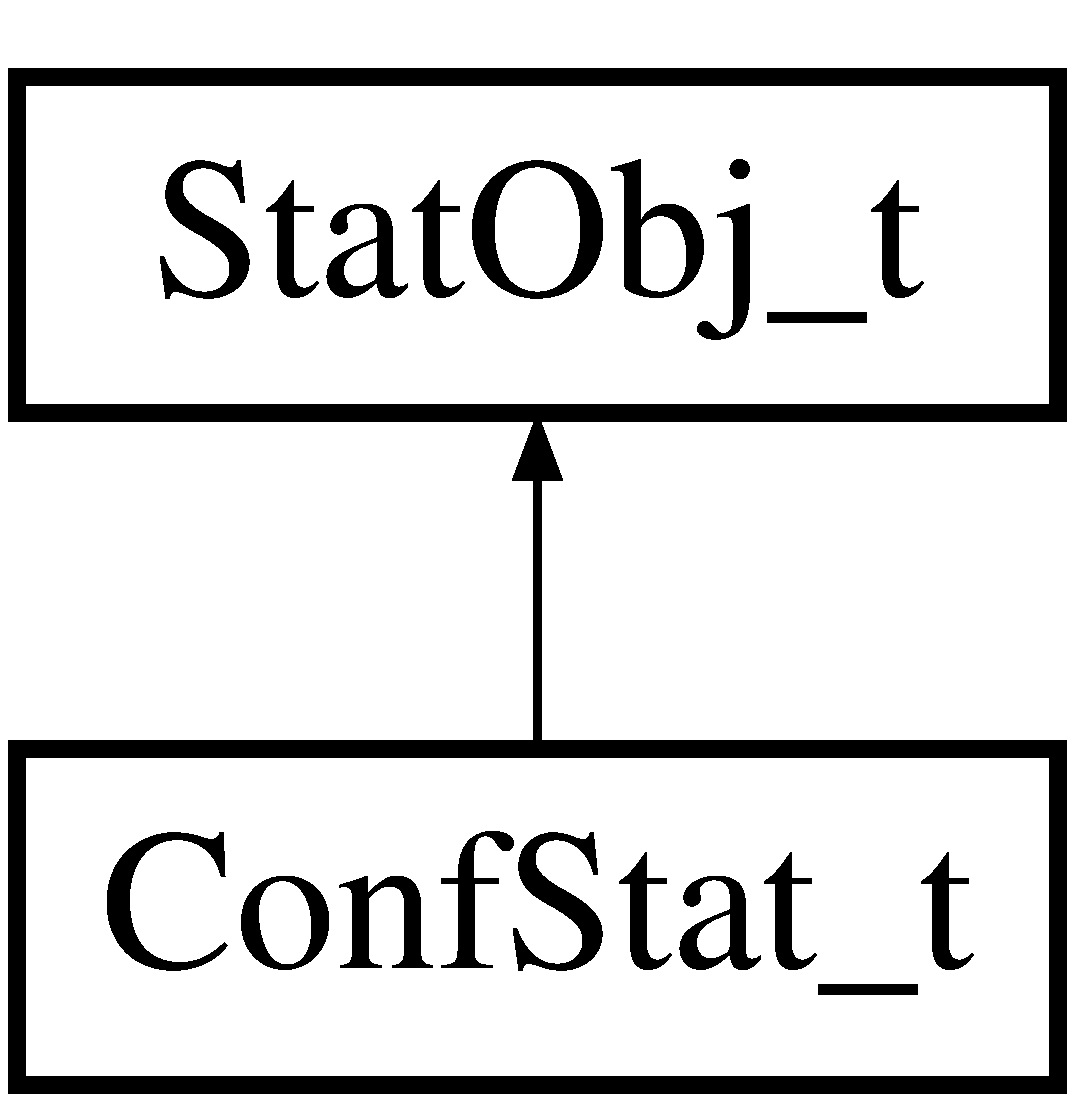
\includegraphics[height=2cm]{classConfStat__t}
\end{center}
\end{figure}
\subsection*{Public Member Functions}
\begin{DoxyCompactItemize}
\item 
void {\bf finish} ()\label{classConfStat__t_a3856ab4b30f39391169a31c27ae15e08}

\begin{DoxyCompactList}\small\item\em Add statistics of the last 10 records. \item\end{DoxyCompactList}\item 
void {\bf printTableHeader} (std::ostream \&out) const \label{classConfStat__t_a26c1d1503dab552f275584065a39e64e}

\begin{DoxyCompactList}\small\item\em Print the table header. \item\end{DoxyCompactList}\item 
void {\bf print} (std::ostream \&out)
\begin{DoxyCompactList}\small\item\em Print the statistics of one object (one table row). \item\end{DoxyCompactList}\item 
bool {\bf hasInfo} () const 
\begin{DoxyCompactList}\small\item\em Return true if at least one error was detected for the corresponding front-\/end. \item\end{DoxyCompactList}\item 
void {\bf addGood} ()
\begin{DoxyCompactList}\small\item\em The configuration data of the corresponding front-\/end is okay. \item\end{DoxyCompactList}\item 
void {\bf addBad} ()
\begin{DoxyCompactList}\small\item\em The configuration data of the corresponding front-\/end is broken. \item\end{DoxyCompactList}\item 
void {\bf addConsecutiveWrites} ()
\begin{DoxyCompactList}\small\item\em The configuration data of the corresponding front-\/end could bot be verified. \item\end{DoxyCompactList}\item 
void {\bf checkPoint} ()\label{classConfStat__t_a46811b871604da482570570dbe654910}

\begin{DoxyCompactList}\small\item\em Add the statistics gathered from the last 10 records to the total statistic and start a fresh sample. \item\end{DoxyCompactList}\item 
void {\bf unCheckedCheckPoint} ()\label{classConfStat__t_af36942046f60ca599e65205e8b00dc6f}

\begin{DoxyCompactList}\small\item\em Add the statistics of the last sample to the total statistic. \item\end{DoxyCompactList}\item 
unsigned int {\bf n} () const \label{classConfStat__t_a8b3afffda1aa70289c51454c3122361d}

\begin{DoxyCompactList}\small\item\em The size of the last sample. \item\end{DoxyCompactList}\item 
unsigned int {\bf bad} () const \label{classConfStat__t_a229df4a06ce1fb0a91c7a9b35da825ee}

\begin{DoxyCompactList}\small\item\em The number of bad configuration records for this front-\/end in the last sample. \item\end{DoxyCompactList}\item 
unsigned int {\bf consecutiveWrites} () const \label{classConfStat__t_a3241e9dcaa3dedf0517f6ec457ceb359}

\begin{DoxyCompactList}\small\item\em The number of unverified configuration records for this front-\/end in the last sample. \item\end{DoxyCompactList}\item 
unsigned int {\bf error} () const \label{classConfStat__t_ae24a58055cd97f82fadaf7d7091c9078}

\begin{DoxyCompactList}\small\item\em The number of configuration errors for this front-\/end in the last sample. \item\end{DoxyCompactList}\item 
unsigned int {\bf nTotal} () const \label{classConfStat__t_a1c97a1c1c9935ad1fecff2eb11c99e74}

\begin{DoxyCompactList}\small\item\em The total sample size. \item\end{DoxyCompactList}\item 
unsigned int {\bf badTotal} () const \label{classConfStat__t_a5bfc54790861399510942d1127f37153}

\begin{DoxyCompactList}\small\item\em The total number of bad configuration records for this front-\/end. \item\end{DoxyCompactList}\item 
unsigned int {\bf consecutiveWritesTotal} () const \label{classConfStat__t_ab098d3d0e143c66ade8900e21d41cd93}

\begin{DoxyCompactList}\small\item\em The total number of unverified configuration records for this front-\/end. \item\end{DoxyCompactList}\end{DoxyCompactItemize}
\subsection*{Private Attributes}
\begin{DoxyCompactItemize}
\item 
unsigned int {\bfseries \_\-n}\label{classConfStat__t_a936050c9f0aa7c50a36c26eb08efbe13}

\item 
unsigned int {\bfseries \_\-feBad}\label{classConfStat__t_a824537e0cc592bfc37d49dd65bafb304}

\item 
unsigned int {\bfseries \_\-consecutiveWrites}\label{classConfStat__t_a8cfcc7feceaf3423270a9fa751d64ed0}

\item 
unsigned int {\bfseries \_\-nTotal}\label{classConfStat__t_a9117a823678b9e6ab33f8573764aa405}

\item 
unsigned int {\bfseries \_\-feBadTotal}\label{classConfStat__t_aa9bcb2f1c6eef1f3bf88bf1e9a5ce756}

\item 
unsigned int {\bfseries \_\-consecutiveWritesTotal}\label{classConfStat__t_ae1a0a81a87e225040d8f642bd52a486f}

\end{DoxyCompactItemize}


\subsection{Detailed Description}
Statistics about configuration record errors. The object is meant to be used together with \doxyref{FeStatList\_\-t}{p.}{classFeStatList__t}. This object collects statistics about bad configuration data. The following errors are counted: the data which is read back does not agree with the data which was written; configuration data was written twice but never read back. \begin{DoxyAuthor}{Author}
Goetz Gaycken, LLR -\/ Ecole polytechnique 
\end{DoxyAuthor}
\begin{DoxyDate}{Date}
feb, 2006 
\end{DoxyDate}


Definition at line 15 of file ConfStatList\_\-t.hh.

\subsection{Member Function Documentation}
\index{ConfStat\_\-t@{ConfStat\_\-t}!addBad@{addBad}}
\index{addBad@{addBad}!ConfStat_t@{ConfStat\_\-t}}
\subsubsection[{addBad}]{\setlength{\rightskip}{0pt plus 5cm}void ConfStat\_\-t::addBad ()\hspace{0.3cm}{\ttfamily  [inline]}}\label{classConfStat__t_a04c8678904ea2a04212d3617117f072b}


The configuration data of the corresponding front-\/end is broken. 

Definition at line 38 of file ConfStatList\_\-t.hh.

References checkPoint().\index{ConfStat\_\-t@{ConfStat\_\-t}!addConsecutiveWrites@{addConsecutiveWrites}}
\index{addConsecutiveWrites@{addConsecutiveWrites}!ConfStat_t@{ConfStat\_\-t}}
\subsubsection[{addConsecutiveWrites}]{\setlength{\rightskip}{0pt plus 5cm}void ConfStat\_\-t::addConsecutiveWrites ()\hspace{0.3cm}{\ttfamily  [inline]}}\label{classConfStat__t_a011c9660b97bec0b7afbc06a7c2b1c65}


The configuration data of the corresponding front-\/end could bot be verified. 

Definition at line 41 of file ConfStatList\_\-t.hh.

References checkPoint().\index{ConfStat\_\-t@{ConfStat\_\-t}!addGood@{addGood}}
\index{addGood@{addGood}!ConfStat_t@{ConfStat\_\-t}}
\subsubsection[{addGood}]{\setlength{\rightskip}{0pt plus 5cm}void ConfStat\_\-t::addGood ()\hspace{0.3cm}{\ttfamily  [inline]}}\label{classConfStat__t_a282d031bbd5b75fd30cef863e4d77060}


The configuration data of the corresponding front-\/end is okay. 

Definition at line 35 of file ConfStatList\_\-t.hh.

References checkPoint().\index{ConfStat\_\-t@{ConfStat\_\-t}!hasInfo@{hasInfo}}
\index{hasInfo@{hasInfo}!ConfStat_t@{ConfStat\_\-t}}
\subsubsection[{hasInfo}]{\setlength{\rightskip}{0pt plus 5cm}bool ConfStat\_\-t::hasInfo () const\hspace{0.3cm}{\ttfamily  [inline, virtual]}}\label{classConfStat__t_a947d830f041d2d38b9f4306d755f470a}


Return true if at least one error was detected for the corresponding front-\/end. 

Implements {\bf StatObj\_\-t} \doxyref{}{p.}{classStatObj__t_a4eb553db0bda3666cab1c390092841a1}.

Definition at line 32 of file ConfStatList\_\-t.hh.

References error().\index{ConfStat\_\-t@{ConfStat\_\-t}!print@{print}}
\index{print@{print}!ConfStat_t@{ConfStat\_\-t}}
\subsubsection[{print}]{\setlength{\rightskip}{0pt plus 5cm}void ConfStat\_\-t::print (std::ostream \& {\em out})\hspace{0.3cm}{\ttfamily  [virtual]}}\label{classConfStat__t_a75a769361503e4adb075bd30aef95f4d}


Print the statistics of one object (one table row). 

Implements {\bf StatObj\_\-t} \doxyref{}{p.}{classStatObj__t_a2763586ba61eb2c37f076e266b0a331e}.

Definition at line 11 of file ConfStatList\_\-t.cc.

References badTotal(), consecutiveWritesTotal(), and nTotal().

The documentation for this class was generated from the following files:\begin{DoxyCompactItemize}
\item 
ConfStatList\_\-t.hh\item 
ConfStatList\_\-t.cc\end{DoxyCompactItemize}

\section{CALICE::ConnCellMappingHcal Class Reference}
\label{classCALICE_1_1ConnCellMappingHcal}\index{CALICE::ConnCellMappingHcal@{CALICE::ConnCellMappingHcal}}


Mapping class based on the LCFixedObject template.  


{\ttfamily \#include $<$ConnCellMappingHcal.hh$>$}\subsection*{Public Member Functions}
\begin{DoxyCompactItemize}
\item 
{\bf ConnCellMappingHcal} (int connpin, int icd\_\-fine, int jcd\_\-fine, int kcd\_\-fine, int icd\_\-coarse, int jcd\_\-coarse, int kcd\_\-coarse)\label{classCALICE_1_1ConnCellMappingHcal_ab42f668b5748b8dfa9b3fc97fa6c7fee}

\begin{DoxyCompactList}\small\item\em Convenient c'tor. \item\end{DoxyCompactList}\item 
{\bf ConnCellMappingHcal} (LCObject $\ast$obj)\label{classCALICE_1_1ConnCellMappingHcal_a081e0f8e841d6f434e17b670cab48d7e}

\begin{DoxyCompactList}\small\item\em 'Copy constructor' needed to interpret LCCollection read from file/database. \item\end{DoxyCompactList}\item 
virtual {\bf $\sim$ConnCellMappingHcal} ()\label{classCALICE_1_1ConnCellMappingHcal_a7a197aeb49859189e104e3d5d94d0391}

\begin{DoxyCompactList}\small\item\em Important for memory handling. \item\end{DoxyCompactList}\item 
int {\bf getConnpin} ()\label{classCALICE_1_1ConnCellMappingHcal_a98cddfbd965baa2a65f830c4b19c9dfc}

\begin{DoxyCompactList}\small\item\em the class interface: \item\end{DoxyCompactList}\item 
int {\bfseries getCellID\_\-fine} ()\label{classCALICE_1_1ConnCellMappingHcal_a86446b579f23ddac044afa98f83be109}

\item 
int {\bfseries getCellID\_\-coarse} ()\label{classCALICE_1_1ConnCellMappingHcal_a8136c2a1622f865fcdab81cda25284e5}

\item 
short {\bf getCellIndex\_\-fine} (std::string)\label{classCALICE_1_1ConnCellMappingHcal_acede8240bf218adff8d40e23d7c7903a}

\begin{DoxyCompactList}\small\item\em convenient getter functions \item\end{DoxyCompactList}\item 
short {\bfseries getCellIndex\_\-coarse} (std::string)\label{classCALICE_1_1ConnCellMappingHcal_aeb22fd5dbacc508100ff4b34d8d6d5e4}

\item 
void {\bfseries print} (std::ostream \&os)\label{classCALICE_1_1ConnCellMappingHcal_ad40f3d45f299b067ba913d53651c9102}

\item 
const std::string {\bf getTypeName} () const \label{classCALICE_1_1ConnCellMappingHcal_a824a0896a35021b8ea42da52c9bfae38}

\begin{DoxyCompactList}\small\item\em Type definition. \item\end{DoxyCompactList}\item 
const std::string {\bfseries getDataDescription} () const \label{classCALICE_1_1ConnCellMappingHcal_a826f2d60b31e3329b5a68dccd014244f}

\end{DoxyCompactItemize}
\subsection*{Private Attributes}
\begin{DoxyCompactItemize}
\item 
short {\bf \_\-index}\label{classCALICE_1_1ConnCellMappingHcal_a63ebe04fafeb25e26b642d38b768cd71}

\begin{DoxyCompactList}\small\item\em i,j or k Index of the cell id \item\end{DoxyCompactList}\end{DoxyCompactItemize}


\subsection{Detailed Description}
Mapping class based on the LCFixedObject template. that relates the mapping of the hcal connectors to the cellids 

Definition at line 33 of file ConnCellMappingHcal.hh.

The documentation for this class was generated from the following files:\begin{DoxyCompactItemize}
\item 
ConnCellMappingHcal.hh\item 
ConnCellMappingHcal.cc\end{DoxyCompactItemize}

\section{CALICE::TriggerHandlerCalice::Crate\_\-t Class Reference}
\label{classCALICE_1_1TriggerHandlerCalice_1_1Crate__t}\index{CALICE::TriggerHandlerCalice::Crate\_\-t@{CALICE::TriggerHandlerCalice::Crate\_\-t}}


Samll helper class which contains a collection of slots and which remebers all the sub detector ids conencted to it.  
\subsection*{Public Member Functions}
\begin{DoxyCompactItemize}
\item 
{\bfseries Crate\_\-t} (unsigned int sub\_\-det\_\-i)\label{classCALICE_1_1TriggerHandlerCalice_1_1Crate__t_a42dd3d017eb1e0981e92f1e57f3605c3}

\item 
bool {\bf isUsed} () const \label{classCALICE_1_1TriggerHandlerCalice_1_1Crate__t_ab0daf2d8f75bf475fb0523c860e6aed1}

\begin{DoxyCompactList}\small\item\em Return true if this crate is connected to at least on known detector. \item\end{DoxyCompactList}\item 
bool {\bf isUsedByMultipleSubDetectors} () const \label{classCALICE_1_1TriggerHandlerCalice_1_1Crate__t_a3141c360228a0a289e147c4a285bb42e}

\begin{DoxyCompactList}\small\item\em Return true if the crate is connected to only one sub detector. \item\end{DoxyCompactList}\item 
void {\bf setSubDetectorID} (unsigned int a\_\-sub\_\-dector)
\begin{DoxyCompactList}\small\item\em Return the ID of the sub detector which is connected to this crate. \item\end{DoxyCompactList}\item 
bool {\bf isConnectedToSubDetector} (unsigned int a\_\-sub\_\-dector) const \label{classCALICE_1_1TriggerHandlerCalice_1_1Crate__t_a00386bdf45d49e71cd8604393b5abc6a}

\begin{DoxyCompactList}\small\item\em Return true if the crate is conencted to the sub detector. \item\end{DoxyCompactList}\item 
{\bf SlotList\_\-t} \& {\bf slotList} ()\label{classCALICE_1_1TriggerHandlerCalice_1_1Crate__t_ab71658dc613ae2c3d5f683d643838567}

\begin{DoxyCompactList}\small\item\em Get the slotlist for read/write access. \item\end{DoxyCompactList}\item 
const {\bf SlotList\_\-t} \& {\bf slotList} () const \label{classCALICE_1_1TriggerHandlerCalice_1_1Crate__t_a9bd990db0cf9d53c6946e697faabd6f7}

\begin{DoxyCompactList}\small\item\em Get the slotlist for read only access. \item\end{DoxyCompactList}\end{DoxyCompactItemize}
\subsection*{Private Attributes}
\begin{DoxyCompactItemize}
\item 
std::vector$<$ unsigned int $>$ {\bfseries \_\-subDetID}\label{classCALICE_1_1TriggerHandlerCalice_1_1Crate__t_a49e7c92525f987ffb4b8b83446935ce1}

\item 
bool {\bfseries \_\-oneDetectorOnly}\label{classCALICE_1_1TriggerHandlerCalice_1_1Crate__t_af6fa23743ffea3d191ab389b996cd6b7}

\item 
{\bf SlotList\_\-t} {\bfseries \_\-slots}\label{classCALICE_1_1TriggerHandlerCalice_1_1Crate__t_af7e308e0893ec31e1d83d54e5856371b}

\end{DoxyCompactItemize}


\subsection{Detailed Description}
Samll helper class which contains a collection of slots and which remebers all the sub detector ids conencted to it. 

Definition at line 569 of file TriggerHandlerCalice.hh.

\subsection{Member Function Documentation}
\index{CALICE::TriggerHandlerCalice::Crate\_\-t@{CALICE::TriggerHandlerCalice::Crate\_\-t}!setSubDetectorID@{setSubDetectorID}}
\index{setSubDetectorID@{setSubDetectorID}!CALICE::TriggerHandlerCalice::Crate_t@{CALICE::TriggerHandlerCalice::Crate\_\-t}}
\subsubsection[{setSubDetectorID}]{\setlength{\rightskip}{0pt plus 5cm}void CALICE::TriggerHandlerCalice::Crate\_\-t::setSubDetectorID (unsigned int {\em a\_\-sub\_\-dector})\hspace{0.3cm}{\ttfamily  [inline]}}\label{classCALICE_1_1TriggerHandlerCalice_1_1Crate__t_a4ad877cf64ba3e78b93d86d21834f281}


Return the ID of the sub detector which is connected to this crate. \begin{DoxySeeAlso}{See also}
set 
\end{DoxySeeAlso}


Definition at line 588 of file TriggerHandlerCalice.hh.

Referenced by CALICE::TriggerHandlerCalice::moduleConnectionChange().

The documentation for this class was generated from the following file:\begin{DoxyCompactItemize}
\item 
TriggerHandlerCalice.hh\end{DoxyCompactItemize}

\section{CALICE::DAQconnection Class Reference}
\label{classCALICE_1_1DAQconnection}\index{CALICE::DAQconnection@{CALICE::DAQconnection}}


Class to store the DAQ address of a singel channel.  


{\ttfamily \#include $<$DAQconnection.hh$>$}\subsection*{Public Member Functions}
\begin{DoxyCompactItemize}
\item 
{\bf DAQconnection} (const unsigned int crate, const unsigned slot, const unsigned int fe, const unsigned int chip, const unsigned int channel, const std::string enc=defaultEncodingString)\label{classCALICE_1_1DAQconnection_a1683f388c10013e8c435262de9c2b0a7}

\begin{DoxyCompactList}\small\item\em Constructor with initial values. \item\end{DoxyCompactList}\item 
{\bf DAQconnection} (EVENT::LCObject $\ast$object, const std::string enc=defaultEncodingString)\label{classCALICE_1_1DAQconnection_a7f6a1f3e76fe54b0f952cccf01b2b489}

\begin{DoxyCompactList}\small\item\em Constructor from LCObject. \item\end{DoxyCompactList}\item 
{\bf $\sim$DAQconnection} ()\label{classCALICE_1_1DAQconnection_aab804c279b14b7139378825152f5d7af}

\begin{DoxyCompactList}\small\item\em Destructor. \item\end{DoxyCompactList}\item 
void {\bfseries setChannel} (unsigned int channel)\label{classCALICE_1_1DAQconnection_abc3d2a36439898873d04493ade4e2b79}

\item 
void {\bfseries setChip} (unsigned int chip)\label{classCALICE_1_1DAQconnection_aa8749c6e343d3703cfd036a8a19851c8}

\item 
void {\bfseries setFe} (unsigned int fe)\label{classCALICE_1_1DAQconnection_abbdb39c30e0d4c1709dc016fabbefabf}

\item 
void {\bfseries setSlot} (unsigned int slot)\label{classCALICE_1_1DAQconnection_a63a06aa5dda5881a3f19135cd5e42bf5}

\item 
void {\bfseries setCrate} (unsigned int crate)\label{classCALICE_1_1DAQconnection_aab13f456fa1e0f793b09820c82d9ada9}

\item 
unsigned int {\bfseries getChannel} () const \label{classCALICE_1_1DAQconnection_a5578725f9868a3c581425eca90fdd223}

\item 
unsigned int {\bfseries getChip} () const \label{classCALICE_1_1DAQconnection_a4a783e2a4d37608d087479dc255731d2}

\item 
unsigned int {\bfseries getFe} () const \label{classCALICE_1_1DAQconnection_ace1feda8e13487780aff0666eaadc83c}

\item 
unsigned int {\bfseries getSlot} () const \label{classCALICE_1_1DAQconnection_af873791c5318dc6496f96c16d1b782a7}

\item 
unsigned int {\bfseries getCrate} () const \label{classCALICE_1_1DAQconnection_a6379ea8cfc3e76ab748acae97e25553b}

\item 
const std::string {\bfseries getEncodingString} () const \label{classCALICE_1_1DAQconnection_aa1ccbcccb16b3ff6ace4b0e31c1d87ff}

\item 
const std::string {\bf getTypeName} () const \label{classCALICE_1_1DAQconnection_a25b1407516b5afd73f813662de211d7e}

\begin{DoxyCompactList}\small\item\em Implementation of LCGenericObject::getTypeName. \item\end{DoxyCompactList}\item 
const std::string {\bf getDataDescription} () const \label{classCALICE_1_1DAQconnection_a7b2b9484febf8612c71291028c6675f4}

\begin{DoxyCompactList}\small\item\em Implementation of LCGenericObject::getDataDescription. \item\end{DoxyCompactList}\end{DoxyCompactItemize}
\subsection*{Private Member Functions}
\begin{DoxyCompactItemize}
\item 
void {\bfseries updateLCobject} ()\label{classCALICE_1_1DAQconnection_a99cde9fbe145d08c6e60ce5946b28814}

\end{DoxyCompactItemize}
\subsection*{Private Attributes}
\begin{DoxyCompactItemize}
\item 
const std::string {\bfseries encodingString}\label{classCALICE_1_1DAQconnection_ae7c2fbe117b63706706a28ac96610975}

\item 
BitField64 {\bfseries bitField}\label{classCALICE_1_1DAQconnection_a98f14d4db56868cecb7b286546a7fe0e}

\end{DoxyCompactItemize}


\subsection{Detailed Description}
Class to store the DAQ address of a singel channel. This class uses the mechanism of the BitField64 to encode and decode the bit positions using a string value. User defined encoding strings are possible. These have to define following fields: \begin{DoxyItemize}
\item crate The crate \item slot Slot in the crate \item fe Frontend on the card in slot \item chip Chip on the frontend \item channel Channel on the chip\end{DoxyItemize}
\begin{DoxyAuthor}{Author}
{\tt Benjamin.Lutz@desy.de} 
\end{DoxyAuthor}
\begin{DoxyVersion}{Version}
1.0 
\end{DoxyVersion}
\begin{DoxyDate}{Date}
September 2008 
\end{DoxyDate}


Definition at line 30 of file DAQconnection.hh.

The documentation for this class was generated from the following files:\begin{DoxyCompactItemize}
\item 
DAQconnection.hh\item 
DAQconnection.cc\end{DoxyCompactItemize}

\section{CALICE::DaqRunSummaryBlock Class Reference}
\label{classCALICE_1_1DaqRunSummaryBlock}\index{CALICE::DaqRunSummaryBlock@{CALICE::DaqRunSummaryBlock}}


Stores a summary of a run in terms of Number of Congfiuration Changes, Slow Readouts, Acquisitions and Number of Events in additions it stores the time of a run and for convenience the run number.  


{\ttfamily \#include $<$DaqRunSummaryBlock.hh$>$}Inheritance diagram for CALICE::DaqRunSummaryBlock::\begin{figure}[H]
\begin{center}
\leavevmode
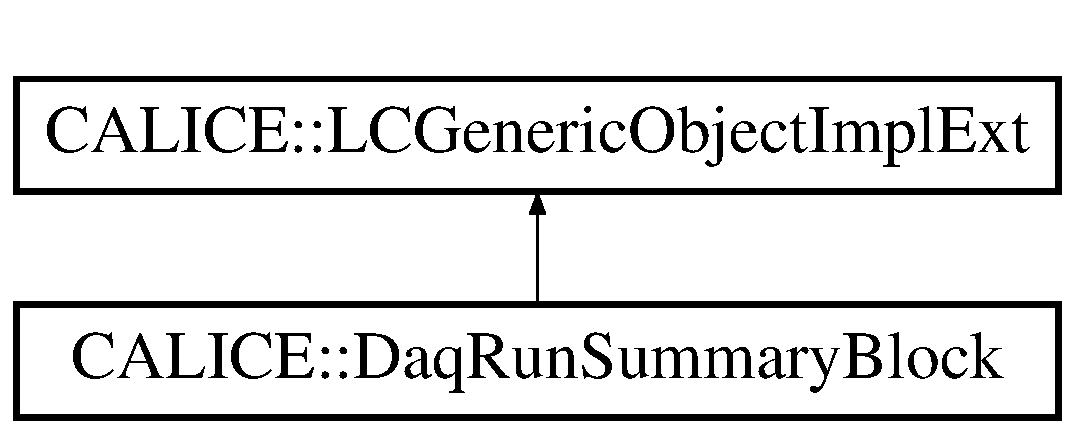
\includegraphics[height=2cm]{classCALICE_1_1DaqRunSummaryBlock}
\end{center}
\end{figure}
\subsection*{Public Member Functions}
\begin{DoxyCompactItemize}
\item 
{\bf DaqRunSummaryBlock} ()\label{classCALICE_1_1DaqRunSummaryBlock_a6fd29ed6330baa493439cdc34e5a3448}

\begin{DoxyCompactList}\small\item\em Default Constructor. \item\end{DoxyCompactList}\item 
{\bf DaqRunSummaryBlock} (LCObject $\ast$obj)\label{classCALICE_1_1DaqRunSummaryBlock_a70bdf0e2b5f667feaf48dd4340c2457c}

\begin{DoxyCompactList}\small\item\em 'Copy constructor' needed to interpret LCCollection read from file/database. \item\end{DoxyCompactList}\item 
{\bf DaqRunSummaryBlock} \& {\bf setRunNumber} (int runnum)\label{classCALICE_1_1DaqRunSummaryBlock_ade14fb40860cd66831ea5401566c0404}

\begin{DoxyCompactList}\small\item\em Set the run number. \item\end{DoxyCompactList}\item 
int {\bf getRunNumber} ()\label{classCALICE_1_1DaqRunSummaryBlock_afdf5fa9bb1dff6475117c66ea60aa103}

\begin{DoxyCompactList}\small\item\em Return the Number of Configurations. \item\end{DoxyCompactList}\item 
{\bf DaqRunSummaryBlock} \& {\bf setNumberOfConfigurations} (int numconf)\label{classCALICE_1_1DaqRunSummaryBlock_aaeb253c0f1165d200dd7bc540cac845a}

\begin{DoxyCompactList}\small\item\em Set the number of configurations. \item\end{DoxyCompactList}\item 
int {\bf getNumberOfConfigurations} ()\label{classCALICE_1_1DaqRunSummaryBlock_ac2bf2eb7f4d0d279cee5a36a690dca83}

\begin{DoxyCompactList}\small\item\em Return the Number of Configurations. \item\end{DoxyCompactList}\item 
{\bf DaqRunSummaryBlock} \& {\bf setNumberOfSlowReadouts} (int numsro)\label{classCALICE_1_1DaqRunSummaryBlock_abed0d403b72287188068448c772b2885}

\begin{DoxyCompactList}\small\item\em Set the number of Slowreadouts. \item\end{DoxyCompactList}\item 
int {\bf getNumberOfSlowReadouts} ()\label{classCALICE_1_1DaqRunSummaryBlock_a0452377daba7afe69a9a4c054f1034d0}

\begin{DoxyCompactList}\small\item\em Get the Number of Slowreadouts. \item\end{DoxyCompactList}\item 
{\bf DaqRunSummaryBlock} \& {\bf setNumberOfAcquisitions} (int numacq)\label{classCALICE_1_1DaqRunSummaryBlock_a5224040c1df1bf17fc0c5ec5bd68f40f}

\begin{DoxyCompactList}\small\item\em Set the number of Acquisitions. \item\end{DoxyCompactList}\item 
int {\bf getNumberOfAcquisitions} ()\label{classCALICE_1_1DaqRunSummaryBlock_acd32c04a0c561e223c71b4d96ba300da}

\begin{DoxyCompactList}\small\item\em Get the Number of Acquisitions. \item\end{DoxyCompactList}\item 
{\bf DaqRunSummaryBlock} \& {\bf setNumberOfEvents} (int numevt)\label{classCALICE_1_1DaqRunSummaryBlock_aee86dd895d3cf1fc0077581aebb5b28e}

\begin{DoxyCompactList}\small\item\em Set the number of Acquisitions. \item\end{DoxyCompactList}\item 
int {\bf getNumberOfEvents} ()\label{classCALICE_1_1DaqRunSummaryBlock_a8c025e9d7f400d419125f66fed82094e}

\begin{DoxyCompactList}\small\item\em Get the Number of Events. \item\end{DoxyCompactList}\item 
{\bf DaqRunSummaryBlock} \& {\bf setRunDuration} (int runtime)\label{classCALICE_1_1DaqRunSummaryBlock_a253c0fb4bdd59cac9285a89e94d2ba5f}

\begin{DoxyCompactList}\small\item\em Set the Run duration. \item\end{DoxyCompactList}\item 
int {\bf getRunDuration} ()\label{classCALICE_1_1DaqRunSummaryBlock_af63f5f6495d45bbc64c5e3b658d593fb}

\begin{DoxyCompactList}\small\item\em Get the Number of Events. \item\end{DoxyCompactList}\item 
void {\bf print} (std::ostream \&os)\label{classCALICE_1_1DaqRunSummaryBlock_a731d6d70fad2033515728de4bb6ba9eb}

\begin{DoxyCompactList}\small\item\em Convenient print method. \item\end{DoxyCompactList}\item 
const std::string {\bf getTypeName} () const \label{classCALICE_1_1DaqRunSummaryBlock_a001a655e6a0b1d141833bae6f4975234}

\begin{DoxyCompactList}\small\item\em Return the type of the class. \item\end{DoxyCompactList}\item 
const std::string {\bf getDataDescription} () const \label{classCALICE_1_1DaqRunSummaryBlock_ac619c2fba39178ba2bb5180ddea1a369}

\begin{DoxyCompactList}\small\item\em Return a brief description of the data members. \item\end{DoxyCompactList}\end{DoxyCompactItemize}


\subsection{Detailed Description}
Stores a summary of a run in terms of Number of Congfiuration Changes, Slow Readouts, Acquisitions and Number of Events in additions it stores the time of a run and for convenience the run number. \begin{DoxySeeAlso}{See also}
\doxyref{ConditionsChangeDelegator}{p.}{classCALICE_1_1ConditionsChangeDelegator} 
\end{DoxySeeAlso}
\begin{DoxyAuthor}{Author}
R. Poeschl LAL (based on the other interface classes)
\end{DoxyAuthor}
\begin{DoxyDate}{Date}
Sep 2007 
\end{DoxyDate}


Definition at line 34 of file DaqRunSummaryBlock.hh.

The documentation for this class was generated from the following files:\begin{DoxyCompactItemize}
\item 
DaqRunSummaryBlock.hh\item 
DaqRunSummaryBlock.cc\end{DoxyCompactItemize}

\section{CALICE::DaqTypeDataBlock Class Reference}
\label{classCALICE_1_1DaqTypeDataBlock}\index{CALICE::DaqTypeDataBlock@{CALICE::DaqTypeDataBlock}}


Base Class to handle all daq types (for the time being apart from the actual crc data) This base class constains the functions to store the data The actual handling of the data is left to dedicated classes which have to derive from this class.  


{\ttfamily \#include $<$DaqTypeDataBlock.hh$>$}Inheritance diagram for CALICE::DaqTypeDataBlock::\begin{figure}[H]
\begin{center}
\leavevmode
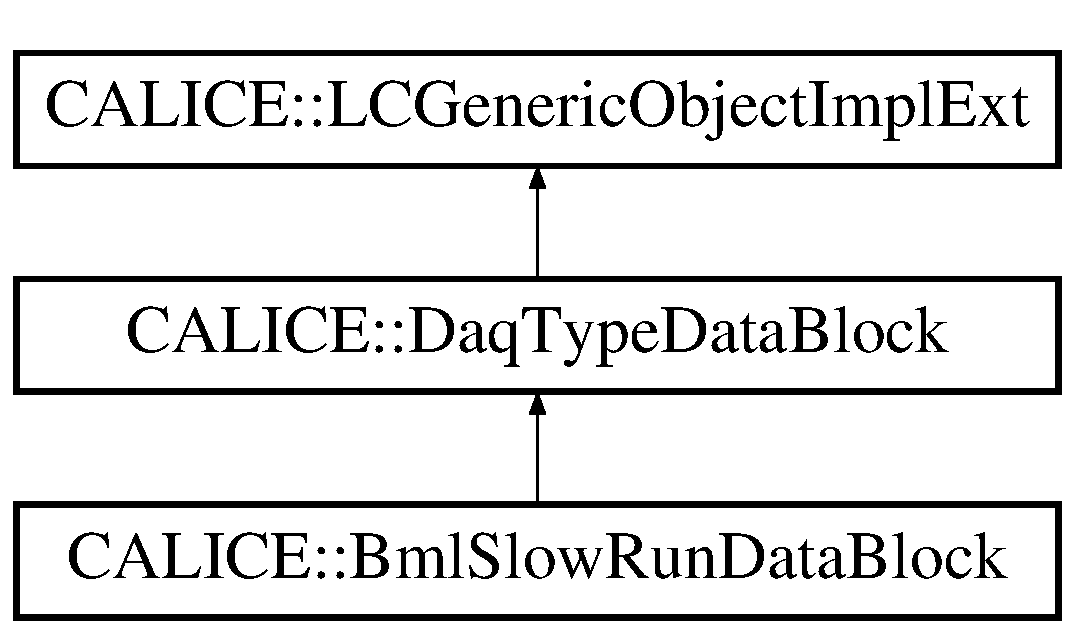
\includegraphics[height=3cm]{classCALICE_1_1DaqTypeDataBlock}
\end{center}
\end{figure}
\subsection*{Public Member Functions}
\begin{DoxyCompactItemize}
\item 
{\bf DaqTypeDataBlock} ()\label{classCALICE_1_1DaqTypeDataBlock_a85c6645ef5c7c0806f3c3df59570f8cc}

\begin{DoxyCompactList}\small\item\em Constructor. \item\end{DoxyCompactList}\item 
{\bf DaqTypeDataBlock} (LCObject $\ast$obj, bool restoreMaps=true)\label{classCALICE_1_1DaqTypeDataBlock_a1e706ee3c127aec373cef65488a6cb9f}

\begin{DoxyCompactList}\small\item\em 'Copy constructor' needed to interpret LCCollection read from file/database. \item\end{DoxyCompactList}\item 
{\bf DaqTypeDataBlock} \& {\bf setTimeStamps} (std::map$<$ std::string, time\_\-t $>$ timeStampMapRaw)\label{classCALICE_1_1DaqTypeDataBlock_aa34e891e8a1fa5bf87f509d4b22cd385}

\begin{DoxyCompactList}\small\item\em Set the time stamps or better initialize the timestamp map which will be stored Remember: We store UTC!!!! \item\end{DoxyCompactList}\item 
{\bf TimeStampMap\_\-t} {\bfseries getTimeStamps} ()\label{classCALICE_1_1DaqTypeDataBlock_a7d275918bef9692d3d514233587a6bf2}

\item 
virtual void {\bf setDblArrays} (const {\bf DaqTypeDataDblMap\_\-t} \&daqTypeDataDblMap)\label{classCALICE_1_1DaqTypeDataBlock_a75a5676e055372817eb4ab644eac3d08}

\begin{DoxyCompactList}\small\item\em These methods receive the vectors with the measured values Mainly to store large arrays of a given datatype but in principle this can be extended to every entry in the interface class. \item\end{DoxyCompactList}\item 
virtual void {\bfseries setFloatArrays} (const DaqTypeDataFloatMap\_\-t \&daqTypeDataFloatMap)\label{classCALICE_1_1DaqTypeDataBlock_a012452bf9295a1cd73d0f7d8634b7253}

\item 
virtual void {\bfseries setIntArrays} (const DaqTypeDataUIntMap\_\-t \&)\label{classCALICE_1_1DaqTypeDataBlock_a98f2ff86e4ad4ba336a1e59ec0ceb34e}

\item 
virtual void {\bfseries setIntArrays} (const DaqTypeDataIntMap\_\-t \&)\label{classCALICE_1_1DaqTypeDataBlock_a134ce924a637904532cc22c1cc0f0ad1}

\item 
DaqTypeDataIntMap\_\-t {\bf getIntArrays} ()
\begin{DoxyCompactList}\small\item\em The following methods allow to retrieve the maps. \item\end{DoxyCompactList}\item 
{\bf DaqTypeDataDblMap\_\-t} {\bfseries getDblArrays} ()\label{classCALICE_1_1DaqTypeDataBlock_a971acc862569f0d3af2aa289b1cb4d5d}

\item 
DaqTypeDataFloatMap\_\-t {\bfseries getFloatArrays} ()\label{classCALICE_1_1DaqTypeDataBlock_a1c9066aad1370879f24f84464fd02da1}

\item 
{\bf DaqTypeDataBlock} $\ast$ {\bf finalize} ()
\begin{DoxyCompactList}\small\item\em A method which finally fills the object which is stored. \item\end{DoxyCompactList}\item 
virtual const double {\bf getBeamEnergy} ()\label{classCALICE_1_1DaqTypeDataBlock_a22c56049653a7e3c0637deadb891e9da}

\begin{DoxyCompactList}\small\item\em A method to calculate the beam energy which has to be implemented by the derived classes. \item\end{DoxyCompactList}\item 
virtual void {\bf print} (std::ostream \&)\label{classCALICE_1_1DaqTypeDataBlock_a0ab5d656a67220cfc75fd842c29e1ac7}

\begin{DoxyCompactList}\small\item\em convenient print method \item\end{DoxyCompactList}\item 
const std::string {\bf getTypeName} () const \label{classCALICE_1_1DaqTypeDataBlock_acb717f063a4de474a5e51924f8d24682}

\begin{DoxyCompactList}\small\item\em Return the type of the class. \item\end{DoxyCompactList}\item 
const std::string {\bf getDataDescription} () const \label{classCALICE_1_1DaqTypeDataBlock_a4dbed57cc9bf006bbd3e670f07fbe2b1}

\begin{DoxyCompactList}\small\item\em Return a brief description of the data members. \item\end{DoxyCompactList}\end{DoxyCompactItemize}
\subsection*{Private Member Functions}
\begin{DoxyCompactItemize}
\item 
void {\bf setNumberOfIntTypes} (int numvals)\label{classCALICE_1_1DaqTypeDataBlock_a28c2c09bb9a1ff30f199188a12ec7bab}

\begin{DoxyCompactList}\small\item\em Store the number of int data types. \item\end{DoxyCompactList}\item 
int {\bf getNumberOfIntTypes} () const \label{classCALICE_1_1DaqTypeDataBlock_adf260ba6c4d5c2178acda6bd6bf329b2}

\begin{DoxyCompactList}\small\item\em Retrieve the number of int data types. \item\end{DoxyCompactList}\item 
void {\bf setNumberOfTimeStamps} (int numvals)\label{classCALICE_1_1DaqTypeDataBlock_a676aad32ad5a5634f384f236495f0ac9}

\begin{DoxyCompactList}\small\item\em Store the number of timestamps. \item\end{DoxyCompactList}\item 
int {\bf getNumberOfTimeStamps} () const \label{classCALICE_1_1DaqTypeDataBlock_a6823cb2b2543bcebb87750ac5423e20e}

\begin{DoxyCompactList}\small\item\em Retrieve the number of int data types. \item\end{DoxyCompactList}\item 
void {\bf setPointerToIndexOfIntTypeNames} (int nameind)\label{classCALICE_1_1DaqTypeDataBlock_ab5c75f5969f61b10ef90801babd1ab1f}

\begin{DoxyCompactList}\small\item\em Store the index at which the pointer to the names of the int data data types do start. \item\end{DoxyCompactList}\item 
int {\bf getPointerToIndexOfIntTypeNames} () const \label{classCALICE_1_1DaqTypeDataBlock_a12176936fc593c6cb09bccc58dff9e25}

\begin{DoxyCompactList}\small\item\em Retrieve the index at which the pointer to the names of int data types do start. \item\end{DoxyCompactList}\item 
void {\bf setPointerToIndexOfTimeStampNames} (int nameind)\label{classCALICE_1_1DaqTypeDataBlock_aac3f7e653792786bc85952f1ea97bba3}

\begin{DoxyCompactList}\small\item\em Store the index at which the pointer to the names of the time stamps do start. \item\end{DoxyCompactList}\item 
int {\bf getPointerToIndexOfTimeStampNames} () const \label{classCALICE_1_1DaqTypeDataBlock_a52e2c8a7356f9b4fe5b0a190df3db19a}

\begin{DoxyCompactList}\small\item\em Retrieve the index at which the pointer to the names of the time stamps do start. \item\end{DoxyCompactList}\item 
void {\bf setTypeIndex} (int pos, int value)\label{classCALICE_1_1DaqTypeDataBlock_a622f0e34c6584942fc1d36c6ab038581}

\begin{DoxyCompactList}\small\item\em Set the index of a given data type name. \item\end{DoxyCompactList}\item 
void {\bf setLengthIndexOfIntTypeNames} (int lengthindex)\label{classCALICE_1_1DaqTypeDataBlock_ab032d6110f9a55ef1f33db4d59197e84}

\begin{DoxyCompactList}\small\item\em Store the index at which the lengths of the names of the int data types do start. \item\end{DoxyCompactList}\item 
int {\bf getLengthIndexOfIntTypeNames} () const \label{classCALICE_1_1DaqTypeDataBlock_a418917055bd74565de117b6c8ff50523}

\begin{DoxyCompactList}\small\item\em Retrieve the index at which the lengths of the names of the int data types do start. \item\end{DoxyCompactList}\item 
void {\bf setLengthIndexOfTimeStampNames} (int lengthindex)\label{classCALICE_1_1DaqTypeDataBlock_afe7ffd23a9d39d2ce552f40227f0f8e6}

\begin{DoxyCompactList}\small\item\em Store the index at which the lengths of the names of the time stamps do start. \item\end{DoxyCompactList}\item 
int {\bf getLengthIndexOfTimeStampNames} () const \label{classCALICE_1_1DaqTypeDataBlock_ae7a837206e4e801f31c5bd22fa0d1017}

\begin{DoxyCompactList}\small\item\em Retrieve the index at which the lengths of the names of the int data types do start. \item\end{DoxyCompactList}\item 
void {\bf setSizeIndexOfIntType} (int size)\label{classCALICE_1_1DaqTypeDataBlock_a96726ed1f53f580959f9ae9f7eb579ca}

\begin{DoxyCompactList}\small\item\em Store the Index where the sizes of the int data data types do start. \item\end{DoxyCompactList}\item 
int {\bf getSizeIndexOfIntType} () const \label{classCALICE_1_1DaqTypeDataBlock_a1f6e0831d20b7f3810ac080517ad7a49}

\begin{DoxyCompactList}\small\item\em Retrieve index where the sizes of int data types do start. \item\end{DoxyCompactList}\item 
void {\bf setNumberOfDblTypes} (int numvals)\label{classCALICE_1_1DaqTypeDataBlock_af22734d9ce54087e2c6b36832668da98}

\begin{DoxyCompactList}\small\item\em Store the number of double data types. \item\end{DoxyCompactList}\item 
int {\bf getNumberOfDblTypes} () const \label{classCALICE_1_1DaqTypeDataBlock_a4f409146da56fcddfbd2495149ea50cd}

\begin{DoxyCompactList}\small\item\em Retrieve the number of double data types. \item\end{DoxyCompactList}\item 
void {\bf setPointerToIndexOfDblTypeNames} (int nameind)\label{classCALICE_1_1DaqTypeDataBlock_a8dbc1b40d1a11be5285a272ee01f597c}

\begin{DoxyCompactList}\small\item\em Store the at which the names the double data data types do start. \item\end{DoxyCompactList}\item 
int {\bf getPointerToIndexOfDblTypeNames} () const \label{classCALICE_1_1DaqTypeDataBlock_a675b5c1436aeba8953a5c569889f1e84}

\begin{DoxyCompactList}\small\item\em Retrieve index at which the names of double data types do start. \item\end{DoxyCompactList}\item 
void {\bf setLengthIndexOfDblTypeNames} (int length)\label{classCALICE_1_1DaqTypeDataBlock_ae8065e890645c324f6740947494fbe06}

\begin{DoxyCompactList}\small\item\em Store the index at which lengths of the names of the double data types do start. \item\end{DoxyCompactList}\item 
int {\bf getLengthIndexOfDblTypeNames} () const \label{classCALICE_1_1DaqTypeDataBlock_ae302a22d40e2e009497ac8ffaaba1a47}

\begin{DoxyCompactList}\small\item\em Retrieve the index at which the lengths of the names of the double data types do start. \item\end{DoxyCompactList}\item 
void {\bf setSizeIndexOfDblType} (int size)\label{classCALICE_1_1DaqTypeDataBlock_ad1c408aae59259c742b2aec8b3517b06}

\begin{DoxyCompactList}\small\item\em Store the Index where the sizes of the double data data types do start. \item\end{DoxyCompactList}\item 
int {\bf getSizeIndexOfDblType} () const \label{classCALICE_1_1DaqTypeDataBlock_a84c98b620f0051e8aeadd93a6f2357b0}

\begin{DoxyCompactList}\small\item\em Retrieve index where the sizes of double data types do start. \item\end{DoxyCompactList}\item 
void {\bf setNumberOfFloatTypes} (int numvals)\label{classCALICE_1_1DaqTypeDataBlock_a841cafcb827e3a396c0554c912240b15}

\begin{DoxyCompactList}\small\item\em Store the number of float data types. \item\end{DoxyCompactList}\item 
int {\bf getNumberOfFloatTypes} () const \label{classCALICE_1_1DaqTypeDataBlock_a0e6f4e46a345d28c63d202d30b744a2e}

\begin{DoxyCompactList}\small\item\em Retrieve the number of float data types. \item\end{DoxyCompactList}\item 
void {\bf setPointerToIndexOfFloatTypeNames} (int nameind)\label{classCALICE_1_1DaqTypeDataBlock_a891466479bac0cbc2b7989808aa90865}

\begin{DoxyCompactList}\small\item\em Store the index at which the names of the float data types do start. \item\end{DoxyCompactList}\item 
int {\bf getPointerToIndexOfFloatTypeNames} () const \label{classCALICE_1_1DaqTypeDataBlock_a153fc0942be078682a9e4a83f4acf3e8}

\begin{DoxyCompactList}\small\item\em Retrieve index at which the names of the float data types do start. \item\end{DoxyCompactList}\item 
void {\bf setLengthIndexOfFloatTypeNames} (int length)\label{classCALICE_1_1DaqTypeDataBlock_a888df6e647e1a5e64a5bd38488315db1}

\begin{DoxyCompactList}\small\item\em Store the index at which the lengths of the names of the float data types do start. \item\end{DoxyCompactList}\item 
int {\bf getLengthIndexOfFloatTypeNames} () const \label{classCALICE_1_1DaqTypeDataBlock_acfc2ef22213129c57bacf00d1e27fa82}

\begin{DoxyCompactList}\small\item\em Retrieve the index at which the lengths of the names of the float data types do start. \item\end{DoxyCompactList}\item 
void {\bf setSizeIndexOfFloatType} (int size)\label{classCALICE_1_1DaqTypeDataBlock_acac139f2e46d4db6af0b6eddd6ec4942}

\begin{DoxyCompactList}\small\item\em Store the Index where the sizes of the float data data types do start. \item\end{DoxyCompactList}\item 
int {\bf getSizeIndexOfFloatType} () const \label{classCALICE_1_1DaqTypeDataBlock_ada9d6720bbd32244e611788b488d8d2a}

\begin{DoxyCompactList}\small\item\em Retrieve index where the sizes of double data types do start. \item\end{DoxyCompactList}\item 
void {\bf calculateTimeStamp} (struct tm $\ast$)\label{classCALICE_1_1DaqTypeDataBlock_a92c758b4cf990905756df438015a061d}

\begin{DoxyCompactList}\small\item\em Simple method to decompose the struct tm containing the timestamp into ints which can be stored in the LCGenericObject and therefore in the database. \item\end{DoxyCompactList}\item 
LCTime {\bf composeTimeStamp} ()\label{classCALICE_1_1DaqTypeDataBlock_a40444b0427fe536b7ea4bf14447a3df8}

\begin{DoxyCompactList}\small\item\em turn the two ints containing the timestamp info into a LCTime Object \item\end{DoxyCompactList}\item 
void {\bf RestoreMaps} ()\label{classCALICE_1_1DaqTypeDataBlock_a57610189b303b049d13ef2b569e5156d}

\begin{DoxyCompactList}\small\item\em A method which restores the map from the generic object. \item\end{DoxyCompactList}\end{DoxyCompactItemize}
\subsection*{Private Attributes}
\begin{DoxyCompactItemize}
\item 
std::map$<$ std::string, time\_\-t $>$ {\bf \_\-timeStampMapRaw}\label{classCALICE_1_1DaqTypeDataBlock_a8867f81834148bdf8a194e71b3b742f8}

\begin{DoxyCompactList}\small\item\em A map holds the nature and the value of the timestamps. \item\end{DoxyCompactList}\item 
{\bf TimeStampMap\_\-t} {\bf \_\-timeStampMap}\label{classCALICE_1_1DaqTypeDataBlock_aa4a278ab29ccecfee83baa22bdc993c0}

\begin{DoxyCompactList}\small\item\em Another map now with the time stamp using LCIO Utils. \item\end{DoxyCompactList}\item 
int {\bf \_\-timestamptoint} [2]\label{classCALICE_1_1DaqTypeDataBlock_a9ca2d41715983eb36a5fc1573d580a9c}

\begin{DoxyCompactList}\small\item\em A simple array which holds the timestamp decomposed into two ints containing a) ymd and b) hms. \item\end{DoxyCompactList}\item 
{\bf DaqTypeDataDblMap\_\-t} {\bf \_\-bufferOfDbls}\label{classCALICE_1_1DaqTypeDataBlock_a95a47d717cbc1a9988d43c37dcb92b43}

\begin{DoxyCompactList}\small\item\em Variables which buffer the maps passed by the converter Buffering is needed since we don't know a priori when the objects are passed to us and which data types they contain the 'finalize' method (see below) will finally create the object from the buffers Buffer for doubles. \item\end{DoxyCompactList}\item 
DaqTypeDataFloatMap\_\-t {\bf \_\-bufferOfFloats}\label{classCALICE_1_1DaqTypeDataBlock_a6bf50fbf5fe6cd66eecffd9e55ce482a}

\begin{DoxyCompactList}\small\item\em Buffer for Floats. \item\end{DoxyCompactList}\item 
DaqTypeDataIntMap\_\-t {\bf \_\-bufferOfInts}\label{classCALICE_1_1DaqTypeDataBlock_ab783f44996aab2ced5c9b2c88a183203}

\begin{DoxyCompactList}\small\item\em Buffer for Ints. \item\end{DoxyCompactList}\end{DoxyCompactItemize}


\subsection{Detailed Description}
Base Class to handle all daq types (for the time being apart from the actual crc data) This base class constains the functions to store the data The actual handling of the data is left to dedicated classes which have to derive from this class. The implementation and the interpretation of the stored values is left to the derived classes. The actual meaning of the entries is propagated from a daq class into the database. Note, that in principle really all data types (apart from crc data) can be handled by this class However, existing interface classes (written before Oct. 2008) will remain untouched or exchanged gradually. if considered to be useful. This class allows for a quick reply to changes in the daq. In particular on the appearance of new data types. \begin{DoxyAuthor}{Author}
: Roman P�schl LAL/Orsay 
\end{DoxyAuthor}
\begin{DoxyDate}{Date}
Oct 2008 
\end{DoxyDate}


Definition at line 61 of file DaqTypeDataBlock.hh.

\subsection{Member Function Documentation}
\index{CALICE::DaqTypeDataBlock@{CALICE::DaqTypeDataBlock}!finalize@{finalize}}
\index{finalize@{finalize}!CALICE::DaqTypeDataBlock@{CALICE::DaqTypeDataBlock}}
\subsubsection[{finalize}]{\setlength{\rightskip}{0pt plus 5cm}{\bf DaqTypeDataBlock} $\ast$ CALICE::DaqTypeDataBlock::finalize ()}\label{classCALICE_1_1DaqTypeDataBlock_a5aac4e6f4aef380287394ad36b30a40d}


A method which finally fills the object which is stored. \begin{Desc}
\item[{\bf Todo}]can the algorithms in this method be templated? \end{Desc}


Definition at line 37 of file DaqTypeDataBlock.cc.

References \_\-bufferOfDbls, \_\-bufferOfFloats, \_\-bufferOfInts, \_\-timeStampMap, \_\-timeStampMapRaw, \_\-timestamptoint, calculateTimeStamp(), CALICE::convertStringToInts(), getLengthIndexOfFloatTypeNames(), getNumberOfDblTypes(), getNumberOfFloatTypes(), getNumberOfIntTypes(), getNumberOfTimeStamps(), getPointerToIndexOfDblTypeNames(), getPointerToIndexOfFloatTypeNames(), getPointerToIndexOfIntTypeNames(), getPointerToIndexOfTimeStampNames(), CALICE::getStringFromInts(), CALICE::LCGenericObjectImplExt::obj(), RestoreMaps(), setLengthIndexOfDblTypeNames(), setLengthIndexOfFloatTypeNames(), setLengthIndexOfIntTypeNames(), setLengthIndexOfTimeStampNames(), setNumberOfDblTypes(), setNumberOfFloatTypes(), setNumberOfIntTypes(), setNumberOfTimeStamps(), setPointerToIndexOfDblTypeNames(), setPointerToIndexOfFloatTypeNames(), setPointerToIndexOfIntTypeNames(), setPointerToIndexOfTimeStampNames(), setSizeIndexOfDblType(), setSizeIndexOfFloatType(), setSizeIndexOfIntType(), and setTypeIndex().\index{CALICE::DaqTypeDataBlock@{CALICE::DaqTypeDataBlock}!getIntArrays@{getIntArrays}}
\index{getIntArrays@{getIntArrays}!CALICE::DaqTypeDataBlock@{CALICE::DaqTypeDataBlock}}
\subsubsection[{getIntArrays}]{\setlength{\rightskip}{0pt plus 5cm}DaqTypeDataIntMap\_\-t CALICE::DaqTypeDataBlock::getIntArrays ()\hspace{0.3cm}{\ttfamily  [inline]}}\label{classCALICE_1_1DaqTypeDataBlock_aed8a8e75c1ca2befbf3f4c1bfe54e0a9}


The following methods allow to retrieve the maps. \begin{Desc}
\item[{\bf Todo}]: Should these methods really be public or only accessible by friend functions or ...? 

: Do we have to check whether they has been filled or not before we hand it to the user? \end{Desc}


Definition at line 120 of file DaqTypeDataBlock.hh.

References \_\-bufferOfInts.

The documentation for this class was generated from the following files:\begin{DoxyCompactItemize}
\item 
DaqTypeDataBlock.hh\item 
DaqTypeDataBlock.cc\end{DoxyCompactItemize}

\section{CALICE::MappedContainer$<$ T $>$::DataWithAddress Class Reference}
\label{classCALICE_1_1MappedContainer_1_1DataWithAddress}\index{CALICE::MappedContainer::DataWithAddress@{CALICE::MappedContainer::DataWithAddress}}
\subsection*{Public Member Functions}
\begin{DoxyCompactItemize}
\item 
{\bfseries DataWithAddress} (const int address, T $\ast$data)\label{classCALICE_1_1MappedContainer_1_1DataWithAddress_ac7e3a4ba88ce83a52f8c8588e6e09f93}

\item 
int {\bfseries getAddress} () const \label{classCALICE_1_1MappedContainer_1_1DataWithAddress_ad2f2af7218488e411b489579955b5abf}

\item 
T $\ast$ {\bfseries getData} () const \label{classCALICE_1_1MappedContainer_1_1DataWithAddress_a9ac16b5083ddc5eb1768db68906583f5}

\end{DoxyCompactItemize}
\subsection*{Private Attributes}
\begin{DoxyCompactItemize}
\item 
int {\bfseries \_\-address}\label{classCALICE_1_1MappedContainer_1_1DataWithAddress_ab31d6a6ecdbf9cbbed05e7ba4d4204cc}

\item 
T $\ast$ {\bfseries \_\-data}\label{classCALICE_1_1MappedContainer_1_1DataWithAddress_a62a77e2b8874fd11ce0c8b065a4e369f}

\end{DoxyCompactItemize}


\subsection{Detailed Description}
\subsubsection*{template$<$class T$>$ class CALICE::MappedContainer$<$ T $>$::DataWithAddress}



Definition at line 249 of file MappedContainer.hh.

The documentation for this class was generated from the following file:\begin{DoxyCompactItemize}
\item 
MappedContainer.hh\end{DoxyCompactItemize}

\section{CALICE::DCIndex Class Reference}
\label{classCALICE_1_1DCIndex}\index{CALICE::DCIndex@{CALICE::DCIndex}}
\subsection*{Public Member Functions}
\begin{DoxyCompactItemize}
\item 
{\bfseries DCIndex} (const unsigned int, const unsigned int, const bool)\label{classCALICE_1_1DCIndex_ad63c29da71e51daf01b7fcd1b5406062}

\item 
const unsigned int {\bfseries DClayer} () const \label{classCALICE_1_1DCIndex_aea8b6f0cca2779514d318bcbd1ef6b7e}

\item 
const unsigned int {\bfseries DCxy} () const \label{classCALICE_1_1DCIndex_a513d6ebf343ab177f8d72ffa17e1fc3b}

\item 
const bool {\bfseries DCnegative} () const \label{classCALICE_1_1DCIndex_a6b0d5449c8e6c7d707e12e4e5ef65c81}

\item 
{\bfseries DCIndex} (const int)\label{classCALICE_1_1DCIndex_accc05b44244c93a41c9213d1e007c7e3}

\item 
const int {\bfseries index} () const \label{classCALICE_1_1DCIndex_a8133a5fb0d7ee839533f9130af9a16ed}

\end{DoxyCompactItemize}
\subsection*{Protected Member Functions}
\begin{DoxyCompactItemize}
\item 
void {\bfseries set} (const unsigned int, const unsigned int, const bool)\label{classCALICE_1_1DCIndex_a20505a45223c4772c74ff7b6969ba7b4}

\end{DoxyCompactItemize}
\subsection*{Private Attributes}
\begin{DoxyCompactItemize}
\item 
int {\bfseries \_\-index}\label{classCALICE_1_1DCIndex_af8b745008558ed0c6d90cdaba50da47f}

\end{DoxyCompactItemize}
\subsection*{Friends}
\begin{DoxyCompactItemize}
\item 
class {\bfseries TdcConnection}\label{classCALICE_1_1DCIndex_ab85618aade64e98c6f7945f78e721566}

\end{DoxyCompactItemize}


\subsection{Detailed Description}


Definition at line 16 of file DCIndex.hh.

The documentation for this class was generated from the following files:\begin{DoxyCompactItemize}
\item 
DCIndex.hh\item 
DCIndex.cc\end{DoxyCompactItemize}

\section{CALICE::DeadNoiseConstants Class Reference}
\label{classCALICE_1_1DeadNoiseConstants}\index{CALICE::DeadNoiseConstants@{CALICE::DeadNoiseConstants}}


Class to store the results of a selection of dead or noisy cells for a certain chip/channel for a fixed moduleID.  


{\ttfamily \#include $<$DeadNoiseConstants.hh$>$}Inheritance diagram for CALICE::DeadNoiseConstants::\begin{figure}[H]
\begin{center}
\leavevmode
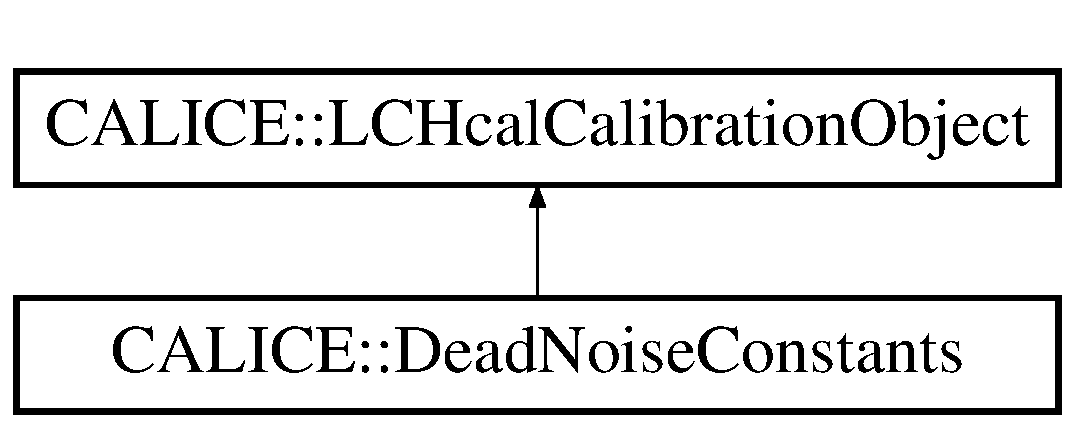
\includegraphics[height=2cm]{classCALICE_1_1DeadNoiseConstants}
\end{center}
\end{figure}
\subsection*{Public Member Functions}
\begin{DoxyCompactItemize}
\item 
{\bf DeadNoiseConstants} ()\label{classCALICE_1_1DeadNoiseConstants_a12212bb9fea94ac0480654f7115f77d7}

\begin{DoxyCompactList}\small\item\em default constructor \item\end{DoxyCompactList}\item 
{\bf DeadNoiseConstants} (unsigned chip, unsigned channel, int deadLevel, int noiseLevel)
\begin{DoxyCompactList}\small\item\em constructor, initializing with parameters \item\end{DoxyCompactList}\item 
{\bfseries DeadNoiseConstants} (LCObject $\ast$obj)\label{classCALICE_1_1DeadNoiseConstants_a8302f5e506b0cf1d98fc2bbb481e4b99}

\item 
int {\bf getDeadLevel} () const \label{classCALICE_1_1DeadNoiseConstants_a10bc03bb0aa616f22eb1f1a734089858}

\begin{DoxyCompactList}\small\item\em get cell dead level \item\end{DoxyCompactList}\item 
float {\bf getNoiseLevel} () const \label{classCALICE_1_1DeadNoiseConstants_aea5232b89fb4db1f000539ac7b85e3e8}

\begin{DoxyCompactList}\small\item\em get cell noise level \item\end{DoxyCompactList}\item 
float {\bf applyCalibration} (float inputValue) const 
\begin{DoxyCompactList}\small\item\em apply calibration to energy value \item\end{DoxyCompactList}\item 
float {\bf applyCalibrationError} (float inputValue, float inputError) const 
\begin{DoxyCompactList}\small\item\em apply calibration error to current error \item\end{DoxyCompactList}\item 
bool {\bf calibrationValid} () const 
\begin{DoxyCompactList}\small\item\em check if a valid calibration is available \item\end{DoxyCompactList}\item 
bool {\bf keepEvent} (float resultValue, float resultError) const 
\begin{DoxyCompactList}\small\item\em accept only non-\/dead and non-\/noisy events \item\end{DoxyCompactList}\item 
void {\bf print} (std::ostream \&os)\label{classCALICE_1_1DeadNoiseConstants_a0c183f8c95da9581b250363ef26b2c21}

\begin{DoxyCompactList}\small\item\em convenient print method \item\end{DoxyCompactList}\item 
const std::string {\bf getTypeName} () const \label{classCALICE_1_1DeadNoiseConstants_a7560a94ebb09e6b925b2988fbeda12e0}

\begin{DoxyCompactList}\small\item\em return type of the class \item\end{DoxyCompactList}\item 
const std::string {\bf getDataDescription} () const \label{classCALICE_1_1DeadNoiseConstants_a618908e466b60a838ecc6667971e6ad2}

\begin{DoxyCompactList}\small\item\em return a brief description of the data member \item\end{DoxyCompactList}\end{DoxyCompactItemize}


\subsection{Detailed Description}
Class to store the results of a selection of dead or noisy cells for a certain chip/channel for a fixed moduleID. \begin{DoxyAuthor}{Author}
S. Schmidt DESY 
\end{DoxyAuthor}
\begin{DoxyDate}{Date}
Sep 25 2006 
\end{DoxyDate}


Definition at line 25 of file DeadNoiseConstants.hh.

\subsection{Constructor \& Destructor Documentation}
\index{CALICE::DeadNoiseConstants@{CALICE::DeadNoiseConstants}!DeadNoiseConstants@{DeadNoiseConstants}}
\index{DeadNoiseConstants@{DeadNoiseConstants}!CALICE::DeadNoiseConstants@{CALICE::DeadNoiseConstants}}
\subsubsection[{DeadNoiseConstants}]{\setlength{\rightskip}{0pt plus 5cm}CALICE::DeadNoiseConstants::DeadNoiseConstants (unsigned {\em chip}, \/  unsigned {\em channel}, \/  int {\em deadLevel}, \/  int {\em noiseLevel})\hspace{0.3cm}{\ttfamily  [inline]}}\label{classCALICE_1_1DeadNoiseConstants_a40bec0935780cdf617c71ca3f46af6a1}


constructor, initializing with parameters 
\begin{DoxyParams}{Parameters}
\item[{\em chip}]chip number of cell to be calibrated \item[{\em channel}]channel number of cell to be calibrated \item[{\em deadLevel}]\char`\"{}level\char`\"{} of being dead for a cell, 0: not dead, 1: dead \item[{\em noiseLevel}]\char`\"{}level\char`\"{} of being noisy for a cell, 0: no noise, 1: low noise, 2: high noise \end{DoxyParams}


Definition at line 39 of file DeadNoiseConstants.hh.

References CALICE::LCHcalCalibrationObject::obj(), and CALICE::LCHcalCalibrationObject::setCellKey().

\subsection{Member Function Documentation}
\index{CALICE::DeadNoiseConstants@{CALICE::DeadNoiseConstants}!applyCalibration@{applyCalibration}}
\index{applyCalibration@{applyCalibration}!CALICE::DeadNoiseConstants@{CALICE::DeadNoiseConstants}}
\subsubsection[{applyCalibration}]{\setlength{\rightskip}{0pt plus 5cm}float CALICE::DeadNoiseConstants::applyCalibration (float {\em inputValue}) const\hspace{0.3cm}{\ttfamily  [inline, virtual]}}\label{classCALICE_1_1DeadNoiseConstants_a117a93e472c84e57b805de35e12b6e29}


apply calibration to energy value 
\begin{DoxyParams}{Parameters}
\item[{\em inputValue}]\char`\"{}energy\char`\"{} value before the calibration \end{DoxyParams}
\begin{DoxyReturn}{Returns}
as the selection of non-\/dead/non-\/noisy cells has no impact on the \char`\"{}energy\char`\"{} the inputValue is returned 
\end{DoxyReturn}


Reimplemented from {\bf CALICE::LCHcalCalibrationObject} \doxyref{}{p.}{classCALICE_1_1LCHcalCalibrationObject_a763f1cf5b9c372fdde268d79b789adcc}.

Definition at line 67 of file DeadNoiseConstants.hh.\index{CALICE::DeadNoiseConstants@{CALICE::DeadNoiseConstants}!applyCalibrationError@{applyCalibrationError}}
\index{applyCalibrationError@{applyCalibrationError}!CALICE::DeadNoiseConstants@{CALICE::DeadNoiseConstants}}
\subsubsection[{applyCalibrationError}]{\setlength{\rightskip}{0pt plus 5cm}float CALICE::DeadNoiseConstants::applyCalibrationError (float {\em inputValue}, \/  float {\em inputError}) const\hspace{0.3cm}{\ttfamily  [inline, virtual]}}\label{classCALICE_1_1DeadNoiseConstants_a1c5558e71e236dabf1e54f54a87162f0}


apply calibration error to current error 
\begin{DoxyParams}{Parameters}
\item[{\em inputValue}]\char`\"{}energy\char`\"{} value before the calibration \item[{\em inputError}]error of the \char`\"{}energy\char`\"{} value before the calibration \end{DoxyParams}
\begin{DoxyReturn}{Returns}
as the selection of non-\/dead/non-\/noisy cells has no error the inputError is returned 
\end{DoxyReturn}


Reimplemented from {\bf CALICE::LCHcalCalibrationObject} \doxyref{}{p.}{classCALICE_1_1LCHcalCalibrationObject_a16d9de9567f68d7784a2daa4d2821341}.

Definition at line 76 of file DeadNoiseConstants.hh.\index{CALICE::DeadNoiseConstants@{CALICE::DeadNoiseConstants}!calibrationValid@{calibrationValid}}
\index{calibrationValid@{calibrationValid}!CALICE::DeadNoiseConstants@{CALICE::DeadNoiseConstants}}
\subsubsection[{calibrationValid}]{\setlength{\rightskip}{0pt plus 5cm}bool CALICE::DeadNoiseConstants::calibrationValid () const\hspace{0.3cm}{\ttfamily  [inline, virtual]}}\label{classCALICE_1_1DeadNoiseConstants_ad7e3bc3298b47d8fa31a43c160a8a45b}


check if a valid calibration is available \begin{DoxyReturn}{Returns}
true as the selection of non-\/dead/non-\/noisy cells is always valid 
\end{DoxyReturn}


Reimplemented from {\bf CALICE::LCHcalCalibrationObject} \doxyref{}{p.}{classCALICE_1_1LCHcalCalibrationObject_abbb1fce81f41a89147b721d593bbc734}.

Definition at line 83 of file DeadNoiseConstants.hh.\index{CALICE::DeadNoiseConstants@{CALICE::DeadNoiseConstants}!keepEvent@{keepEvent}}
\index{keepEvent@{keepEvent}!CALICE::DeadNoiseConstants@{CALICE::DeadNoiseConstants}}
\subsubsection[{keepEvent}]{\setlength{\rightskip}{0pt plus 5cm}bool CALICE::DeadNoiseConstants::keepEvent (float {\em resultValue}, \/  float {\em resultError}) const\hspace{0.3cm}{\ttfamily  [inline, virtual]}}\label{classCALICE_1_1DeadNoiseConstants_af4318e256ff1466682855553d5ba453e}


accept only non-\/dead and non-\/noisy events 
\begin{DoxyParams}{Parameters}
\item[{\em resultValue}]\char`\"{}energy\char`\"{} value after the calibration \item[{\em resultError}]error of the \char`\"{}energy\char`\"{} value after the calibration \end{DoxyParams}
\begin{DoxyReturn}{Returns}
true if a cell is non-\/dead and non-\/noisy 
\end{DoxyReturn}


Reimplemented from {\bf CALICE::LCHcalCalibrationObject} \doxyref{}{p.}{classCALICE_1_1LCHcalCalibrationObject_a59f14a6b83e77717751ae4e7213e8d09}.

Definition at line 92 of file DeadNoiseConstants.hh.

References getDeadLevel(), and getNoiseLevel().

The documentation for this class was generated from the following files:\begin{DoxyCompactItemize}
\item 
DeadNoiseConstants.hh\item 
DeadNoiseConstants.cc\end{DoxyCompactItemize}

\section{CALICE::DecoderSet Class Reference}
\label{classCALICE_1_1DecoderSet}\index{CALICE::DecoderSet@{CALICE::DecoderSet}}


class containing decoders for the three \doxyref{CALICE}{p.}{namespaceCALICE} coordinate systems  


{\ttfamily \#include $<$DecoderSet.hh$>$}\subsection*{Data Structures}
\begin{DoxyCompactItemize}
\item 
struct {\bf MokkaID\_\-t}
\end{DoxyCompactItemize}
\subsection*{Public Member Functions}
\begin{DoxyCompactItemize}
\item 
{\bf DecoderSet} ()
\begin{DoxyCompactList}\small\item\em standard constructor \item\end{DoxyCompactList}\item 
{\bf DecoderSet} (const std::string \&cellIDencoding, const std::string \&moduleEncoding, const std::string \&DAQencoding)
\begin{DoxyCompactList}\small\item\em constructor with encoding strings \item\end{DoxyCompactList}\item 
void {\bf setCellIDEncoding} (const std::string \&encoding)
\begin{DoxyCompactList}\small\item\em set a new cell ID encoding string if an empty string is given the function will use the default encoding string \item\end{DoxyCompactList}\item 
void {\bf setModuleEncoding} (const std::string \&encoding)
\begin{DoxyCompactList}\small\item\em set a new Module tile encoding string if an empty string is given the function will use the default encoding string \item\end{DoxyCompactList}\item 
void {\bf setDAQEncoding} (const std::string \&encoding)
\begin{DoxyCompactList}\small\item\em set a new DAQ channel ID encoding string if an empty string is given the function will use the default encoding string \item\end{DoxyCompactList}\item 
const std::string \& {\bf getCellIDEncoding} () const 
\begin{DoxyCompactList}\small\item\em get the current cell ID encoding string \item\end{DoxyCompactList}\item 
const std::string \& {\bf getModuleEncoding} () const 
\begin{DoxyCompactList}\small\item\em get the current Module tile encoding string \item\end{DoxyCompactList}\item 
const std::string \& {\bf getDAQEncoding} () const 
\begin{DoxyCompactList}\small\item\em get the current DAQ channel ID encoding string \item\end{DoxyCompactList}\item 
unsigned int {\bf getIFromCellID} (const int cellID) const 
\begin{DoxyCompactList}\small\item\em get I from (Mokka) CellID The right encoding string has to be set before. \item\end{DoxyCompactList}\item 
unsigned int {\bf getJFromCellID} (const int cellID) const 
\begin{DoxyCompactList}\small\item\em get J from (Mokka) CellID The right encoding string has to be set before. \item\end{DoxyCompactList}\item 
unsigned int {\bf getKFromCellID} (const int cellID) const 
\begin{DoxyCompactList}\small\item\em get K from (Mokka) CellID The right encoding string has to be set before. \item\end{DoxyCompactList}\item 
unsigned int {\bf getModuleFromModuleID} (const int moduleID) const 
\begin{DoxyCompactList}\small\item\em get module from (Module) channel ID The right encoding string has to be set before. \item\end{DoxyCompactList}\item 
unsigned int {\bf getChipFromModuleID} (const int moduleID) const 
\begin{DoxyCompactList}\small\item\em get chip from (Module) channel ID The right encoding string has to be set before. \item\end{DoxyCompactList}\item 
unsigned int {\bf getChannelFromModuleID} (const int moduleID) const 
\begin{DoxyCompactList}\small\item\em get channel from (Module) channel ID The right encoding string has to be set before. \item\end{DoxyCompactList}\item 
unsigned int {\bf getChannelFromDAQID} (const int {\bf DAQconnection}) const 
\begin{DoxyCompactList}\small\item\em get channel from DAQ channel ID The right encoding string has to be set before. \item\end{DoxyCompactList}\item 
unsigned int {\bf getChipFromDAQID} (const int {\bf DAQconnection}) const 
\begin{DoxyCompactList}\small\item\em get chip from DAQ channel ID The right encoding string has to be set before. \item\end{DoxyCompactList}\item 
unsigned int {\bf getFeFromDAQID} (const int {\bf DAQconnection}) const 
\begin{DoxyCompactList}\small\item\em get fe from DAQ channel ID The right encoding string has to be set before. \item\end{DoxyCompactList}\item 
unsigned int {\bf getSlotFromDAQID} (const int {\bf DAQconnection}) const 
\begin{DoxyCompactList}\small\item\em get slot from DAQ channel ID The right encoding string has to be set before. \item\end{DoxyCompactList}\item 
unsigned int {\bf getCrateFromDAQID} (const int {\bf DAQconnection}) const 
\begin{DoxyCompactList}\small\item\em get crate from DAQ channel ID The right encoding string has to be set before. \item\end{DoxyCompactList}\item 
int {\bf getCellID} (const unsigned int I, const unsigned int J, const unsigned int K) const 
\begin{DoxyCompactList}\small\item\em get CellID from triple I,J,K \item\end{DoxyCompactList}\item 
int {\bf getModuleID} (const unsigned int module, const unsigned int chip, const unsigned int channel) const 
\begin{DoxyCompactList}\small\item\em get (Module) channel ID from triple module, chip, channel \item\end{DoxyCompactList}\item 
int {\bf getDAQID} (const unsigned int crate, const unsigned int slot, const unsigned int fe, const unsigned int chip, const unsigned int channel) const 
\begin{DoxyCompactList}\small\item\em get DAQ channel ID from crate, slot, fe, chip, channel \item\end{DoxyCompactList}\end{DoxyCompactItemize}
\subsection*{Private Types}
\begin{DoxyCompactItemize}
\item 
typedef std::map$<$ std::string, {\bf MokkaID\_\-t} $>$ {\bfseries mokkaDecoderMap\_\-t}\label{classCALICE_1_1DecoderSet_aaa60db49451c3183f3b44c7738a3eb2e}

\end{DoxyCompactItemize}
\subsection*{Private Attributes}
\begin{DoxyCompactItemize}
\item 
std::string {\bfseries \_\-cellIDencodingString}\label{classCALICE_1_1DecoderSet_adabb4fa6971abdefb51e793dbd4afc80}

\item 
std::string {\bfseries \_\-moduleIDEncodingString}\label{classCALICE_1_1DecoderSet_a00fe23b51254c77dbc495dcec6075447}

\item 
std::string {\bfseries \_\-daqIDencodingString}\label{classCALICE_1_1DecoderSet_a1b8a88e2732336e6ac7a80acdf7d6f62}

\item 
{\bf FastDecoder} $\ast$ {\bfseries \_\-IFromCellID}\label{classCALICE_1_1DecoderSet_af543cade302a4724ddba67b313c39f76}

\item 
{\bf FastDecoder} $\ast$ {\bfseries \_\-JFromCellID}\label{classCALICE_1_1DecoderSet_a5c6c387c762f0e425e7477ee9cbb759e}

\item 
{\bf FastDecoder} $\ast$ {\bfseries \_\-KFromCellID}\label{classCALICE_1_1DecoderSet_acc617bd3d0f5ea5de5634c552d6c0d7c}

\item 
{\bf FastDecoder} $\ast$ {\bfseries \_\-moduleFromModuleID}\label{classCALICE_1_1DecoderSet_a480f62a678cdd42278f315455607a8dd}

\item 
{\bf FastDecoder} $\ast$ {\bfseries \_\-chipFromModuleID}\label{classCALICE_1_1DecoderSet_a8c22d248c09b54673a5333da4c410047}

\item 
{\bf FastDecoder} $\ast$ {\bfseries \_\-channelFromModuleID}\label{classCALICE_1_1DecoderSet_a5f7a75f6f5e1c663a9791c0bee9588a4}

\item 
{\bf FastDecoder} $\ast$ {\bfseries \_\-channelFromDAQID}\label{classCALICE_1_1DecoderSet_a943d0f42488e4aa6e3f965b0508578a4}

\item 
{\bf FastDecoder} $\ast$ {\bfseries \_\-chipFromDAQID}\label{classCALICE_1_1DecoderSet_ac11c29224b62198eec4305ca1dfadb6a}

\item 
{\bf FastDecoder} $\ast$ {\bfseries \_\-feFromDAQID}\label{classCALICE_1_1DecoderSet_a4c210127405c95009fe59cae8182c176}

\item 
{\bf FastDecoder} $\ast$ {\bfseries \_\-slotFromDAQID}\label{classCALICE_1_1DecoderSet_afe00087e59c1dad5fc1b6cf09e4fa943}

\item 
{\bf FastDecoder} $\ast$ {\bfseries \_\-crateFromDAQID}\label{classCALICE_1_1DecoderSet_ab968ef239f7ccf67e78b4c0d25be38df}

\item 
mokkaDecoderMap\_\-t {\bfseries \_\-mokkaDecoderMap}\label{classCALICE_1_1DecoderSet_a2264ad82f9cb4b731218d02e6d99d592}

\end{DoxyCompactItemize}
\subsection*{Static Private Attributes}
\begin{DoxyCompactItemize}
\item 
static const std::string {\bfseries \_\-defaultCellIDEncoding}\label{classCALICE_1_1DecoderSet_a416bb066df00dfe53a1220a22610a19e}

\item 
static const std::string {\bfseries \_\-defaultModuleEncoding}\label{classCALICE_1_1DecoderSet_a54a834f1bb6537816d7f5b5d88a36cac}

\item 
static const std::string {\bfseries \_\-defaultDAQEncoding}\label{classCALICE_1_1DecoderSet_a35f02dd35c4b49c13eea9a1c4ff5ca92}

\end{DoxyCompactItemize}


\subsection{Detailed Description}
class containing decoders for the three \doxyref{CALICE}{p.}{namespaceCALICE} coordinate systems \begin{DoxyAuthor}{Author}
{\tt Benjamin.Lutz@desy.de} 
\end{DoxyAuthor}
\begin{DoxyVersion}{Version}
0.1 
\end{DoxyVersion}
\begin{DoxyDate}{Date}
November 2009 
\end{DoxyDate}


Definition at line 36 of file DecoderSet.hh.

\subsection{Constructor \& Destructor Documentation}
\index{CALICE::DecoderSet@{CALICE::DecoderSet}!DecoderSet@{DecoderSet}}
\index{DecoderSet@{DecoderSet}!CALICE::DecoderSet@{CALICE::DecoderSet}}
\subsubsection[{DecoderSet}]{\setlength{\rightskip}{0pt plus 5cm}CALICE::DecoderSet::DecoderSet ()}\label{classCALICE_1_1DecoderSet_a743f5958009c0c90f3be15eb073f155d}


standard constructor encoding strings will be initialised to defaults 

Definition at line 10 of file DecoderSet.cc.

References setCellIDEncoding(), setDAQEncoding(), and setModuleEncoding().\index{CALICE::DecoderSet@{CALICE::DecoderSet}!DecoderSet@{DecoderSet}}
\index{DecoderSet@{DecoderSet}!CALICE::DecoderSet@{CALICE::DecoderSet}}
\subsubsection[{DecoderSet}]{\setlength{\rightskip}{0pt plus 5cm}CALICE::DecoderSet::DecoderSet (const std::string \& {\em cellIDencoding}, \/  const std::string \& {\em moduleEncoding}, \/  const std::string \& {\em DAQencoding})}\label{classCALICE_1_1DecoderSet_a239661518de0a223cd7214c5bf49e69c}


constructor with encoding strings 
\begin{DoxyParams}{Parameters}
\item[\mbox{$\leftarrow$} {\em cellIDencoding}]encoding string for (Mokka) cell IDs \item[\mbox{$\leftarrow$} {\em moduleEncoding}]encoding string for module channel ID \item[\mbox{$\leftarrow$} {\em DAQencoding}]encoding string for DAQ channel ID \end{DoxyParams}


Definition at line 21 of file DecoderSet.cc.

References setCellIDEncoding(), setDAQEncoding(), and setModuleEncoding().

The documentation for this class was generated from the following files:\begin{DoxyCompactItemize}
\item 
DecoderSet.hh\item 
DecoderSet.cc\end{DoxyCompactItemize}

\section{CALICE::DetectorTransformation Class Reference}
\label{classCALICE_1_1DetectorTransformation}\index{CALICE::DetectorTransformation@{CALICE::DetectorTransformation}}


Define the experimental setup: beam energy, position, angle and detector position, angle.  


{\ttfamily \#include $<$DetectorTransformation.hh$>$}\subsection*{Public Member Functions}
\begin{DoxyCompactItemize}
\item 
{\bf DetectorTransformation} (LCObject $\ast$obj)\label{classCALICE_1_1DetectorTransformation_aa0cecf48097264a6a6cc0af071008d0b}

\begin{DoxyCompactList}\small\item\em 'Copy constructor' needed to interpret LCCollection read from file/database. \item\end{DoxyCompactList}\item 
{\bf DetectorTransformation} \& {\bf setDetectorAngleZX} (float detector\_\-angle\_\-zx)
\begin{DoxyCompactList}\small\item\em Set the angle of the detector w.r.t. \item\end{DoxyCompactList}\item 
float {\bf getDetectorAngleZX} () const 
\begin{DoxyCompactList}\small\item\em Get the angle of the detector w.r.t. \item\end{DoxyCompactList}\item 
{\bf DetectorTransformation} \& {\bf setDetectorRotationX0} (float rotation\_\-origin\_\-x0)\label{classCALICE_1_1DetectorTransformation_a2eef8fc060f0844f2c58dd406e236dcf}

\begin{DoxyCompactList}\small\item\em Set the origin of the detector rotation in the ZX-\/plane. \item\end{DoxyCompactList}\item 
float {\bf getDetectorRotationX0} () const \label{classCALICE_1_1DetectorTransformation_afcbf82cfdf8f7e59f8eb9d0dbbcacaf2}

\begin{DoxyCompactList}\small\item\em Get the origin of the detector rotation in the ZX-\/plane. \item\end{DoxyCompactList}\item 
{\bf DetectorTransformation} \& {\bf setDetectorRotationZ0} (float rotation\_\-origin\_\-z0)\label{classCALICE_1_1DetectorTransformation_aec6ee5baab95ce9cb39df88ca04e0e80}

\begin{DoxyCompactList}\small\item\em Set the origin of the detector rotation in the ZX-\/plane. \item\end{DoxyCompactList}\item 
float {\bf getDetectorRotationZ0} () const \label{classCALICE_1_1DetectorTransformation_afd32ba2a1636520f713cee65d6f5b5dc}

\begin{DoxyCompactList}\small\item\em Get the origin of the detector rotation in the ZX-\/plane. \item\end{DoxyCompactList}\item 
{\bf DetectorTransformation} \& {\bf setDetectorTransformation} (float origin\_\-x0, float origin\_\-y0, float origin\_\-z0)\label{classCALICE_1_1DetectorTransformation_aff20896660ff50a94ffe067ccdc56ac6}

\begin{DoxyCompactList}\small\item\em Set the origin of the detector in the 3D-\/space (convenience method). \item\end{DoxyCompactList}\item 
{\bf DetectorTransformation} \& {\bf setDetectorTransformation} (float $\ast$origin\_\-three\_\-vector)\label{classCALICE_1_1DetectorTransformation_ae390bbf318d5747c72d77b6cd364540b}

\begin{DoxyCompactList}\small\item\em Set the origin of the detector in the 3D-\/space (convenience method). \item\end{DoxyCompactList}\item 
{\bf DetectorTransformation} \& {\bf setDetectorX0} (float origin\_\-x0)\label{classCALICE_1_1DetectorTransformation_a12be9cd46f36fbd4995afb93b0001630}

\begin{DoxyCompactList}\small\item\em Set the origin of the detector in the 3D-\/space. \item\end{DoxyCompactList}\item 
float {\bf getDetectorX0} () const \label{classCALICE_1_1DetectorTransformation_ad3b792347abe29df128864f8d93db90b}

\begin{DoxyCompactList}\small\item\em Get the origin of the detector in the 3D-\/space. \item\end{DoxyCompactList}\item 
{\bf DetectorTransformation} \& {\bf setDetectorY0} (float origin\_\-y0)\label{classCALICE_1_1DetectorTransformation_a8aa19f83e78ce547f6144b0ca055f5b4}

\begin{DoxyCompactList}\small\item\em Set the origin of the detector in the 3D-\/space. \item\end{DoxyCompactList}\item 
float {\bf getDetectorY0} () const \label{classCALICE_1_1DetectorTransformation_a8b40f70eab9c5f3f7246d881757fc8e9}

\begin{DoxyCompactList}\small\item\em Get the origin of the detector in the 3D-\/space. \item\end{DoxyCompactList}\item 
{\bf DetectorTransformation} \& {\bf setDetectorZ0} (float origin\_\-z0)\label{classCALICE_1_1DetectorTransformation_a74831156933ee18369f6ea48d90e8f29}

\begin{DoxyCompactList}\small\item\em Set the origin of the detector in the 3D-\/space. \item\end{DoxyCompactList}\item 
float {\bf getDetectorZ0} () const \label{classCALICE_1_1DetectorTransformation_aed697370c5d136d4424867598c79421d}

\begin{DoxyCompactList}\small\item\em Get the origin of the detector in the 3D-\/space. \item\end{DoxyCompactList}\item 
void {\bf print} (std::ostream \&os)\label{classCALICE_1_1DetectorTransformation_a53146e49344a9995016d521d423959fc}

\begin{DoxyCompactList}\small\item\em Print all members (for debugging). \item\end{DoxyCompactList}\item 
const std::string {\bf getTypeName} () const \label{classCALICE_1_1DetectorTransformation_a32750bb0d4ebc5fe3a62871a4b6a427a}

\begin{DoxyCompactList}\small\item\em Return the type of the class. \item\end{DoxyCompactList}\item 
const std::string {\bf getDataDescription} () const \label{classCALICE_1_1DetectorTransformation_a5c2acba9e28ad26da43444e39bc220a7}

\begin{DoxyCompactList}\small\item\em Return a brief description of the data members. \item\end{DoxyCompactList}\end{DoxyCompactItemize}


\subsection{Detailed Description}
Define the experimental setup: beam energy, position, angle and detector position, angle. The experimental setup should be written into the conditions database at least twice: 
\begin{DoxyItemize}
\item the nominal values with the tag NOMINAL 
\item the measured values 
\end{DoxyItemize}\begin{Desc}
\item[{\bf Todo}]\{Should this class be split into two? One for the beam and one for the detector parameters? Should the nominal and measured values be stored in separate folders?\} \end{Desc}


Definition at line 37 of file DetectorTransformation.hh.

\subsection{Member Function Documentation}
\index{CALICE::DetectorTransformation@{CALICE::DetectorTransformation}!getDetectorAngleZX@{getDetectorAngleZX}}
\index{getDetectorAngleZX@{getDetectorAngleZX}!CALICE::DetectorTransformation@{CALICE::DetectorTransformation}}
\subsubsection[{getDetectorAngleZX}]{\setlength{\rightskip}{0pt plus 5cm}float CALICE::DetectorTransformation::getDetectorAngleZX () const\hspace{0.3cm}{\ttfamily  [inline]}}\label{classCALICE_1_1DetectorTransformation_a457ff79d33057315b535678a89c93baa}


Get the angle of the detector w.r.t. z-\/axis in the ZX-\/plane. 

Definition at line 56 of file DetectorTransformation.hh.

References CALICE::kDetectorTransformationFloatDetectorAngleZX.

Referenced by CALICE::CellDescriptionGenerator::generate(), and print().\index{CALICE::DetectorTransformation@{CALICE::DetectorTransformation}!setDetectorAngleZX@{setDetectorAngleZX}}
\index{setDetectorAngleZX@{setDetectorAngleZX}!CALICE::DetectorTransformation@{CALICE::DetectorTransformation}}
\subsubsection[{setDetectorAngleZX}]{\setlength{\rightskip}{0pt plus 5cm}{\bf DetectorTransformation}\& CALICE::DetectorTransformation::setDetectorAngleZX (float {\em detector\_\-angle\_\-zx})\hspace{0.3cm}{\ttfamily  [inline]}}\label{classCALICE_1_1DetectorTransformation_abda40c896fba1eb47056f69774f058b0}


Set the angle of the detector w.r.t. z-\/axis in the ZX-\/plane. 

Definition at line 48 of file DetectorTransformation.hh.

References CALICE::kDetectorTransformationFloatDetectorAngleZX.

The documentation for this class was generated from the following files:\begin{DoxyCompactItemize}
\item 
DetectorTransformation.hh\item 
DetectorTransformation.cc\end{DoxyCompactItemize}

\section{CALICE::DhcRawChipContent Class Reference}
\label{classCALICE_1_1DhcRawChipContent}\index{CALICE::DhcRawChipContent@{CALICE::DhcRawChipContent}}


Simple class which stores the dhcal chip content Note that the dchal as it is now delivers the same time stamp for \_\-all\_\- 64 channels served by a chip.  


{\ttfamily \#include $<$DhcRawChipContent.hh$>$}Inheritance diagram for CALICE::DhcRawChipContent::\begin{figure}[H]
\begin{center}
\leavevmode
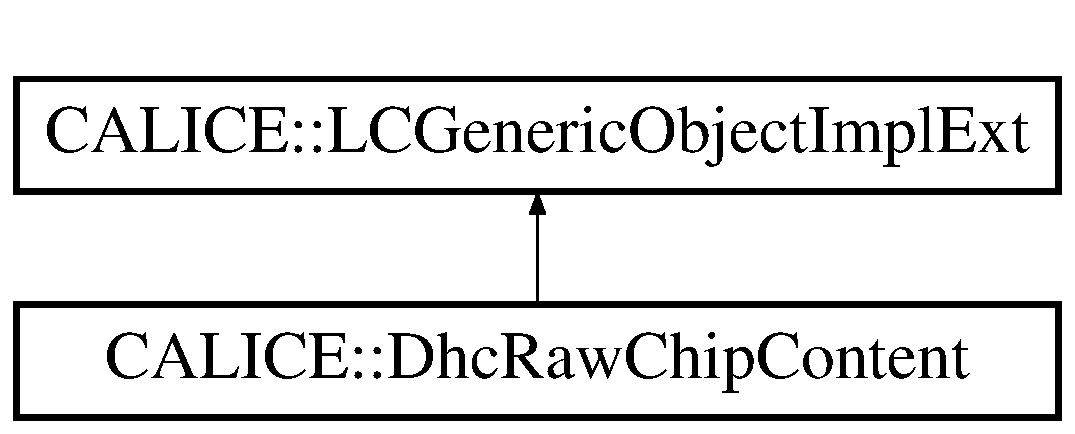
\includegraphics[height=2cm]{classCALICE_1_1DhcRawChipContent}
\end{center}
\end{figure}
\subsection*{Public Member Functions}
\begin{DoxyCompactItemize}
\item 
{\bf DhcRawChipContent} ()\label{classCALICE_1_1DhcRawChipContent_a40a38cc72c861a07276425e293834915}

\begin{DoxyCompactList}\small\item\em Simple Constructor. \item\end{DoxyCompactList}\item 
{\bf DhcRawChipContent} (LCObject $\ast$obj)
\begin{DoxyCompactList}\small\item\em 'Copy constructor' needed to interpret LCCollection read from file/database. \item\end{DoxyCompactList}\item 
virtual {\bf $\sim$DhcRawChipContent} ()\label{classCALICE_1_1DhcRawChipContent_a118479e64dcaa1578df4c2b5b5305fc5}

\begin{DoxyCompactList}\small\item\em The destructor. \item\end{DoxyCompactList}\item 
{\bf DhcRawChipContent} \& {\bf setCrateNumber} (unsigned int cratenr)\label{classCALICE_1_1DhcRawChipContent_ae648a73206346a7e435b190c31503533}

\begin{DoxyCompactList}\small\item\em Set the high hits. \item\end{DoxyCompactList}\item 
unsigned int {\bfseries getCrateNumber} () const \label{classCALICE_1_1DhcRawChipContent_ac38db7829bb2e4ce117bf6bff30b5e30}

\item 
{\bf DhcRawChipContent} \& {\bf setElecChannel} (unsigned int vmead, unsigned int dcalad, unsigned int dcolad, unsigned int dconad)\label{classCALICE_1_1DhcRawChipContent_ad15611d95fe8f56da1df10bafd42a869}

\begin{DoxyCompactList}\small\item\em Set the electronic channel number. \item\end{DoxyCompactList}\item 
int {\bf getElecChannel} () const \label{classCALICE_1_1DhcRawChipContent_a835846130132c03bd9c55a52fcca0baf}

\begin{DoxyCompactList}\small\item\em Get the entire electronic channel number. \item\end{DoxyCompactList}\item 
unsigned int {\bf getVmeAddress} () const \label{classCALICE_1_1DhcRawChipContent_a41b24b4a3aab879318b7bb73bc0abf3d}

\begin{DoxyCompactList}\small\item\em Return the addresses of individual hardware components. \item\end{DoxyCompactList}\item 
unsigned int {\bfseries getDcalAddress} () const \label{classCALICE_1_1DhcRawChipContent_a7c3eeeebac537abaa903e594c2719eb5}

\item 
unsigned int {\bfseries getDcolAddress} () const \label{classCALICE_1_1DhcRawChipContent_a69c7bd11fccade453f965629bf664dd7}

\item 
unsigned int {\bfseries getDconAddress} () const \label{classCALICE_1_1DhcRawChipContent_a17b53680be279714c856302fd1932bc0}

\item 
{\bf DhcRawChipContent} \& {\bf setHitsHi} (unsigned int hitshi)\label{classCALICE_1_1DhcRawChipContent_a65d1a25cfdca13308dfdd0e1b101c468}

\begin{DoxyCompactList}\small\item\em Set the high hits. \item\end{DoxyCompactList}\item 
unsigned int {\bfseries getHitsHi} () const \label{classCALICE_1_1DhcRawChipContent_a154d9d95875b10420c5c3bab19098e47}

\item 
{\bf DhcRawChipContent} \& {\bf setHitsLo} (unsigned int hitslo)\label{classCALICE_1_1DhcRawChipContent_a8a0aa0c0b062f58866ad6d8c6d641652}

\begin{DoxyCompactList}\small\item\em Set the low hits. \item\end{DoxyCompactList}\item 
unsigned int {\bf getHitsLo} () const \label{classCALICE_1_1DhcRawChipContent_a41c5e80b718bb2aaf5367c5506bf5f1d}

\begin{DoxyCompactList}\small\item\em Return the low hits. \item\end{DoxyCompactList}\item 
{\bf DhcRawChipContent} \& {\bf setDhcTimeStamp} (unsigned int timestamp)\label{classCALICE_1_1DhcRawChipContent_ac0e10fb580cc00b0f4b0a3efdd956b91}

\begin{DoxyCompactList}\small\item\em The core, the time stamp. \item\end{DoxyCompactList}\item 
unsigned int {\bf getDhcTimeStamp} () const \label{classCALICE_1_1DhcRawChipContent_a784ab74d557fa360154d0116f8448d03}

\begin{DoxyCompactList}\small\item\em Return the time stamp. \item\end{DoxyCompactList}\item 
{\bf DhcRawChipContent} \& {\bf setMiscInfo} (bool trg, bool dbt, unsigned char err, unsigned char chksum, unsigned char versum)\label{classCALICE_1_1DhcRawChipContent_abed887f844826b95fe369701a8b6719d}

\begin{DoxyCompactList}\small\item\em Set miscalleneous information. \item\end{DoxyCompactList}\item 
bool {\bf getTrgInfo} ()\label{classCALICE_1_1DhcRawChipContent_a7c93aa3a5eb24d81067e2d4059869435}

\begin{DoxyCompactList}\small\item\em Return the trigger information. \item\end{DoxyCompactList}\item 
bool {\bf getDbtInfo} ()\label{classCALICE_1_1DhcRawChipContent_a26fb65c45f4a3b07d779e442069477f2}

\begin{DoxyCompactList}\small\item\em Return the dbt information. \item\end{DoxyCompactList}\item 
unsigned char {\bf getErrInfo} ()\label{classCALICE_1_1DhcRawChipContent_af6261bc47ae47a360632fb0079d4bc99}

\begin{DoxyCompactList}\small\item\em Return the error information. \item\end{DoxyCompactList}\item 
unsigned char {\bf getChkSum} ()\label{classCALICE_1_1DhcRawChipContent_aa9a55ba4880c7b03db55c3728980f44d}

\begin{DoxyCompactList}\small\item\em Return the checksum information. \item\end{DoxyCompactList}\item 
unsigned char {\bf getVerSum} ()\label{classCALICE_1_1DhcRawChipContent_a469cbbfed09f4f5a7e1bc3775b6240e9}

\begin{DoxyCompactList}\small\item\em Return the verification sum (to check checksum). \item\end{DoxyCompactList}\item 
std::ostream \& {\bf print} (std::ostream \&ostrm)\label{classCALICE_1_1DhcRawChipContent_a555dbb9e80d6bb86d0d0092231109ebe}

\begin{DoxyCompactList}\small\item\em Convenient print method. \item\end{DoxyCompactList}\item 
const std::string {\bfseries getTypeName} () const \label{classCALICE_1_1DhcRawChipContent_a3a5fd3f86e153a64edcbeb444001f5aa}

\item 
const std::string {\bf getDataDescription} () const \label{classCALICE_1_1DhcRawChipContent_af28eebdb0ad0ce1f8be17f191b714ef0}

\begin{DoxyCompactList}\small\item\em Return a brief description of the data members. \item\end{DoxyCompactList}\end{DoxyCompactItemize}


\subsection{Detailed Description}
Simple class which stores the dhcal chip content Note that the dchal as it is now delivers the same time stamp for \_\-all\_\- 64 channels served by a chip. That's why the LCIO RawCalorimeterHit class is not convenient. Since it would lead to an increas of the data volume by a factor 64.

\begin{DoxyAuthor}{Author}
R. P�schl (LAL Orsay) 
\end{DoxyAuthor}
\begin{DoxyDate}{Date}
Dec 2010 
\end{DoxyDate}


Definition at line 56 of file DhcRawChipContent.hh.

\subsection{Constructor \& Destructor Documentation}
\index{CALICE::DhcRawChipContent@{CALICE::DhcRawChipContent}!DhcRawChipContent@{DhcRawChipContent}}
\index{DhcRawChipContent@{DhcRawChipContent}!CALICE::DhcRawChipContent@{CALICE::DhcRawChipContent}}
\subsubsection[{DhcRawChipContent}]{\setlength{\rightskip}{0pt plus 5cm}CALICE::DhcRawChipContent::DhcRawChipContent (LCObject $\ast$ {\em obj})\hspace{0.3cm}{\ttfamily  [inline]}}\label{classCALICE_1_1DhcRawChipContent_aa7c59fb4dd3447fb4968bff83ae2e72d}


'Copy constructor' needed to interpret LCCollection read from file/database. 

Definition at line 73 of file DhcRawChipContent.hh.

The documentation for this class was generated from the following files:\begin{DoxyCompactItemize}
\item 
DhcRawChipContent.hh\item 
DhcRawChipContent.cc\end{DoxyCompactItemize}

\section{CALICE::DhcReadoutConfBlock Class Reference}
\label{classCALICE_1_1DhcReadoutConfBlock}\index{CALICE::DhcReadoutConfBlock@{CALICE::DhcReadoutConfBlock}}


Class to interface the configuration of the Dhcal fes.  


{\ttfamily \#include $<$DhcReadoutConfBlock.hh$>$}Inheritance diagram for CALICE::DhcReadoutConfBlock::\begin{figure}[H]
\begin{center}
\leavevmode
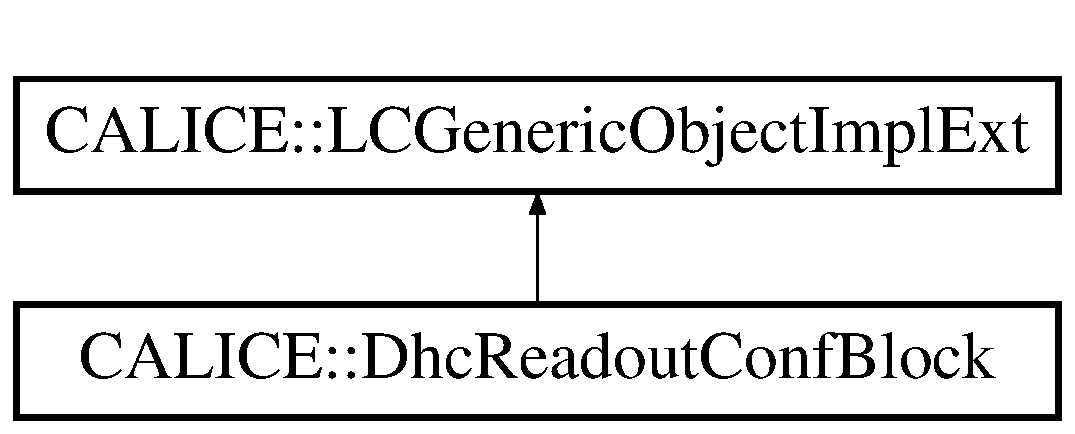
\includegraphics[height=2cm]{classCALICE_1_1DhcReadoutConfBlock}
\end{center}
\end{figure}
\subsection*{Public Member Functions}
\begin{DoxyCompactItemize}
\item 
{\bf DhcReadoutConfBlock} ()\label{classCALICE_1_1DhcReadoutConfBlock_a70a6203130f321b808bfd840623d9e7f}

\begin{DoxyCompactList}\small\item\em Simple Constructor. \item\end{DoxyCompactList}\item 
{\bf DhcReadoutConfBlock} (LCObject $\ast$obj)
\begin{DoxyCompactList}\small\item\em 'Copy constructor' needed to interpret LCCollection read from file/database. \item\end{DoxyCompactList}\item 
virtual {\bf $\sim$DhcReadoutConfBlock} ()\label{classCALICE_1_1DhcReadoutConfBlock_a1765688be6fb5c820ad7403b700b4462}

\begin{DoxyCompactList}\small\item\em The destructor. \item\end{DoxyCompactList}\item 
{\bf DhcReadoutConfBlock} \& {\bf setNumbers} (unsigned int numbers)\label{classCALICE_1_1DhcReadoutConfBlock_ae23cae3a4b8e9a5390e67a8a9022d401}

\begin{DoxyCompactList}\small\item\em Set the numbers. \item\end{DoxyCompactList}\item 
unsigned int {\bf getNumbers} () const \label{classCALICE_1_1DhcReadoutConfBlock_a9f32a07abeb6b9231c893af87d489458}

\begin{DoxyCompactList}\small\item\em Get the numbers. \item\end{DoxyCompactList}\item 
unsigned int {\bf getCrateNumber} ()\label{classCALICE_1_1DhcReadoutConfBlock_a780bef3bacec82f4b3526eb27c2d7115}

\begin{DoxyCompactList}\small\item\em Return the crate number, can be obtained from numbers. \item\end{DoxyCompactList}\item 
{\bf DhcReadoutConfBlock} \& {\bf setSlotEnableMask} (unsigned int slotenablemask)\label{classCALICE_1_1DhcReadoutConfBlock_afa415eb6133bf1c69058c298322770d6}

\begin{DoxyCompactList}\small\item\em Set the slot enable mask, which tells which slots in could (in principle) have been enabled. \item\end{DoxyCompactList}\item 
unsigned int {\bf getSlotEnableMask} () const \label{classCALICE_1_1DhcReadoutConfBlock_af6c73aac10efdf9b040b3f7c129b460d}

\begin{DoxyCompactList}\small\item\em Get the slot enable mask. \item\end{DoxyCompactList}\item 
{\bf DhcReadoutConfBlock} \& {\bf setSlotEnable} (unsigned int slotenable)
\begin{DoxyCompactList}\small\item\em Set the slot enable, i.e. \item\end{DoxyCompactList}\item 
unsigned int {\bf getSlotEnable} () const \label{classCALICE_1_1DhcReadoutConfBlock_a3b7ff51d37ea0eb0d9fd28483d4f4d05}

\begin{DoxyCompactList}\small\item\em Get the slot enable. \item\end{DoxyCompactList}\item 
{\bf DhcReadoutConfBlock} \& {\bf setNumberOfSlots} (unsigned int numslots)\label{classCALICE_1_1DhcReadoutConfBlock_aa8c67bc9f9b615951ffaeb1322780870}

\begin{DoxyCompactList}\small\item\em Set the number of slots, note that this number will have to be multiplied by two, leave it for the time being. \item\end{DoxyCompactList}\item 
unsigned int {\bf getNumberOfSlots} () const \label{classCALICE_1_1DhcReadoutConfBlock_ade3ff579b72a62e49ffb1ac2eb5d4af0}

\begin{DoxyCompactList}\small\item\em Get the numbers of slots. \item\end{DoxyCompactList}\item 
{\bf DhcReadoutConfBlock} \& {\bf setSlotFeEnable} (unsigned int islot, unsigned int val)\label{classCALICE_1_1DhcReadoutConfBlock_a86d81715bb55e049b0165413b5dd78e7}

\begin{DoxyCompactList}\small\item\em Set the enabled fes for this slot. \item\end{DoxyCompactList}\item 
unsigned short {\bf getSlotFeEnable} (unsigned int islot)\label{classCALICE_1_1DhcReadoutConfBlock_a6dfd32e97665265a42e265be9adaad72}

\begin{DoxyCompactList}\small\item\em Get the enabled fes for this slot. \item\end{DoxyCompactList}\item 
{\bf DhcReadoutConfBlock} \& {\bf setSlotFeRevision} (unsigned int islot, unsigned char val)\label{classCALICE_1_1DhcReadoutConfBlock_a50394d95d1b8a5645fd20aea51eab985}

\begin{DoxyCompactList}\small\item\em Set the revision number of the fes for this slot. \item\end{DoxyCompactList}\item 
unsigned char {\bf getSlotFeRevision} (unsigned int islot)\label{classCALICE_1_1DhcReadoutConfBlock_a6e3a476cb7b0bfb8f873f560061ac359}

\begin{DoxyCompactList}\small\item\em Set the revision number of the fes for this slot. \item\end{DoxyCompactList}\item 
{\bf DhcReadoutConfBlock} \& {\bf setBeWaitInterval} (unsigned int timeinmus)\label{classCALICE_1_1DhcReadoutConfBlock_a2c55d4268e15f6d729b6c137e84a7ce9}

\begin{DoxyCompactList}\small\item\em Set the Be wait interval. \item\end{DoxyCompactList}\item 
LCTime {\bf getBeWaitInterval} ()\label{classCALICE_1_1DhcReadoutConfBlock_aee430b699617c6f5455097a665d479dd}

\begin{DoxyCompactList}\small\item\em Return the Be wait interval, in mus. \item\end{DoxyCompactList}\item 
std::ostream \& {\bf print} (std::ostream \&ostrm)\label{classCALICE_1_1DhcReadoutConfBlock_a8ee86e4066e289a3b7c8ac19af5cb45c}

\begin{DoxyCompactList}\small\item\em Convenient print method. \item\end{DoxyCompactList}\item 
const std::string {\bfseries getTypeName} () const \label{classCALICE_1_1DhcReadoutConfBlock_a634f76ea5b591f421b31605ef247b1c4}

\item 
const std::string {\bf getDataDescription} () const \label{classCALICE_1_1DhcReadoutConfBlock_a13be0777aff947ce444b20b25b53720e}

\begin{DoxyCompactList}\small\item\em Return a brief description of the data members. \item\end{DoxyCompactList}\end{DoxyCompactItemize}
\subsection*{Private Member Functions}
\begin{DoxyCompactItemize}
\item 
void {\bf fillSlotToWordsAssociationMask} (unsigned int, bool)
\begin{DoxyCompactList}\small\item\em Association mask. \item\end{DoxyCompactList}\item 
void {\bf fillMethod} (unsigned int, unsigned int, unsigned int, unsigned int)\label{classCALICE_1_1DhcReadoutConfBlock_a593c9ef319474740dba7dc0c723d5dac}

\begin{DoxyCompactList}\small\item\em A convenient method to fill fe eanble and fe revision values. \item\end{DoxyCompactList}\item 
unsigned short {\bf getMethod} (unsigned int, unsigned int, unsigned int)\label{classCALICE_1_1DhcReadoutConfBlock_a7b5d00a1093812e7eee3fc1a67798138}

\begin{DoxyCompactList}\small\item\em A convenient method to fill fe eanble and fe revision values. \item\end{DoxyCompactList}\end{DoxyCompactItemize}
\subsection*{Private Attributes}
\begin{DoxyCompactItemize}
\item 
std::map$<$ unsigned int, unsigned int $>$ {\bf \_\-islotfillMap}\label{classCALICE_1_1DhcReadoutConfBlock_abce693038d694ce51fb6cde002c4dd60}

\begin{DoxyCompactList}\small\item\em map which associates the slots with the position in the LCGenericObject \item\end{DoxyCompactList}\item 
bool {\bf \_\-numSlotsInitialised}\label{classCALICE_1_1DhcReadoutConfBlock_ae767a99973ecf078a438c5c80e4f3019}

\begin{DoxyCompactList}\small\item\em is the number of slots initialised (makes only sense during the filling sequence) \item\end{DoxyCompactList}\end{DoxyCompactItemize}


\subsection{Detailed Description}
Class to interface the configuration of the Dhcal fes. \begin{DoxyAuthor}{Author}
R. P�schl (LAL Orsay), J. Smith (ANL) 
\end{DoxyAuthor}
\begin{DoxyDate}{Date}
Apr 2011 
\end{DoxyDate}
\begin{Desc}
\item[{\bf Todo}]Attention we may introduce a platform dependency here!!!! The structure of the object assumes that LCGenericObjects are aligned on 32 bits Need maybe revision for assumptions on data alignment, could be added as collection parameters, \end{Desc}


Definition at line 32 of file DhcReadoutConfBlock.hh.

\subsection{Constructor \& Destructor Documentation}
\index{CALICE::DhcReadoutConfBlock@{CALICE::DhcReadoutConfBlock}!DhcReadoutConfBlock@{DhcReadoutConfBlock}}
\index{DhcReadoutConfBlock@{DhcReadoutConfBlock}!CALICE::DhcReadoutConfBlock@{CALICE::DhcReadoutConfBlock}}
\subsubsection[{DhcReadoutConfBlock}]{\setlength{\rightskip}{0pt plus 5cm}CALICE::DhcReadoutConfBlock::DhcReadoutConfBlock (LCObject $\ast$ {\em obj})\hspace{0.3cm}{\ttfamily  [inline]}}\label{classCALICE_1_1DhcReadoutConfBlock_a7d4faa50c5595058596fde44971854ab}


'Copy constructor' needed to interpret LCCollection read from file/database. 

Definition at line 48 of file DhcReadoutConfBlock.hh.

References \_\-numSlotsInitialised, fillSlotToWordsAssociationMask(), and getSlotEnableMask().

\subsection{Member Function Documentation}
\index{CALICE::DhcReadoutConfBlock@{CALICE::DhcReadoutConfBlock}!fillSlotToWordsAssociationMask@{fillSlotToWordsAssociationMask}}
\index{fillSlotToWordsAssociationMask@{fillSlotToWordsAssociationMask}!CALICE::DhcReadoutConfBlock@{CALICE::DhcReadoutConfBlock}}
\subsubsection[{fillSlotToWordsAssociationMask}]{\setlength{\rightskip}{0pt plus 5cm}void DhcReadoutConfBlock::fillSlotToWordsAssociationMask (unsigned int {\em slotenablemask}, \/  bool {\em initvals})\hspace{0.3cm}{\ttfamily  [private]}}\label{classCALICE_1_1DhcReadoutConfBlock_ae090fa9e9abbbd1156220bff23b0293c}


Association mask. 

using the slot enable mask we create the map which associates the slots to the position in the LCGenericObject 

Definition at line 21 of file DhcReadoutConfBlock.cc.

References \_\-islotfillMap, \_\-numSlotsInitialised, getNumberOfSlots(), and CALICE::LCGenericObjectImplExt::obj().

Referenced by DhcReadoutConfBlock(), and setSlotEnableMask().\index{CALICE::DhcReadoutConfBlock@{CALICE::DhcReadoutConfBlock}!setSlotEnable@{setSlotEnable}}
\index{setSlotEnable@{setSlotEnable}!CALICE::DhcReadoutConfBlock@{CALICE::DhcReadoutConfBlock}}
\subsubsection[{setSlotEnable}]{\setlength{\rightskip}{0pt plus 5cm}{\bf DhcReadoutConfBlock}\& CALICE::DhcReadoutConfBlock::setSlotEnable (unsigned int {\em slotenable})\hspace{0.3cm}{\ttfamily  [inline]}}\label{classCALICE_1_1DhcReadoutConfBlock_a3c77ac14bc825e8e14ec2346547c5ce4}


Set the slot enable, i.e. the slots which are really enabled 

Definition at line 92 of file DhcReadoutConfBlock.hh.

References CALICE::LCGenericObjectImplExt::obj().

The documentation for this class was generated from the following files:\begin{DoxyCompactItemize}
\item 
DhcReadoutConfBlock.hh\item 
DhcReadoutConfBlock.cc\end{DoxyCompactItemize}

\section{CALICE::DifTrigger Class Reference}
\label{classCALICE_1_1DifTrigger}\index{CALICE::DifTrigger@{CALICE::DifTrigger}}


Simple class which stores the trigger counter retrieved from the DIF cards.  


{\ttfamily \#include $<$DifTrigger.hh$>$}Inheritance diagram for CALICE::DifTrigger::\begin{figure}[H]
\begin{center}
\leavevmode
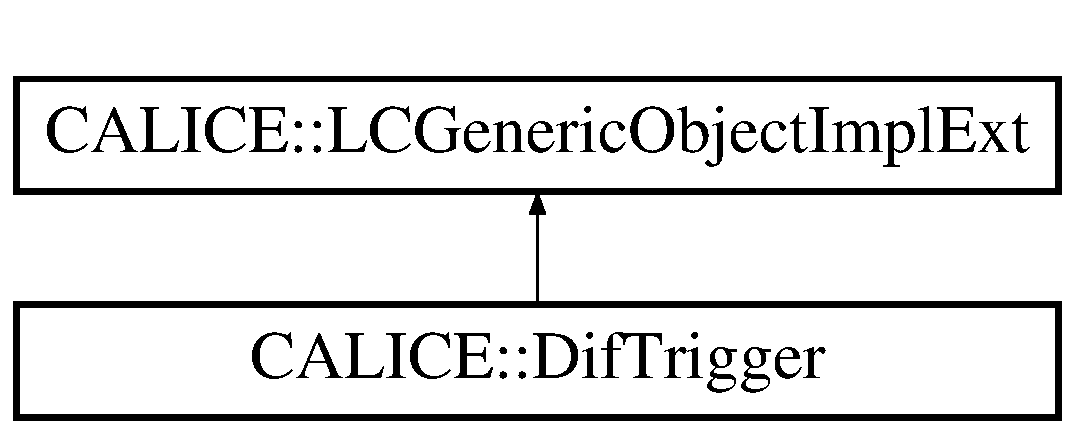
\includegraphics[height=2cm]{classCALICE_1_1DifTrigger}
\end{center}
\end{figure}
\subsection*{Public Member Functions}
\begin{DoxyCompactItemize}
\item 
{\bf DifTrigger} ()\label{classCALICE_1_1DifTrigger_a6b7e84ec0cf67f3aea3f44e32ab976f1}

\begin{DoxyCompactList}\small\item\em Simple Constructor. \item\end{DoxyCompactList}\item 
{\bf DifTrigger} (LCObject $\ast$obj)
\begin{DoxyCompactList}\small\item\em 'Copy constructor' needed to interpret LCCollection read from file/database. \item\end{DoxyCompactList}\item 
virtual {\bf $\sim$DifTrigger} ()\label{classCALICE_1_1DifTrigger_abb5e9c8b0f17ad4a0dc0885640ede48f}

\begin{DoxyCompactList}\small\item\em The destructor. \item\end{DoxyCompactList}\item 
{\bf DifTrigger} \& {\bf setTriggerCounter} (int triggercounter)\label{classCALICE_1_1DifTrigger_abed77f4943569ab3e5e1abf1280f7fe5}

\begin{DoxyCompactList}\small\item\em Set the trigger counter. \item\end{DoxyCompactList}\item 
int {\bf getTriggerCounter} () const \label{classCALICE_1_1DifTrigger_a1a369c606a8c7a935c10f154b8d8f967}

\begin{DoxyCompactList}\small\item\em Get the trigger counter. \item\end{DoxyCompactList}\item 
std::ostream \& {\bf print} (std::ostream \&ostrm)\label{classCALICE_1_1DifTrigger_aa029e99b0d09472495e640a1a10bcf27}

\begin{DoxyCompactList}\small\item\em Convenient print method. \item\end{DoxyCompactList}\item 
const std::string {\bfseries getTypeName} () const \label{classCALICE_1_1DifTrigger_abdf381d1c077acd671f35d18d69a7b1a}

\item 
const std::string {\bf getDataDescription} () const \label{classCALICE_1_1DifTrigger_a24d4a28eb189d634f917db3152340d5a}

\begin{DoxyCompactList}\small\item\em Return a brief description of the data members. \item\end{DoxyCompactList}\end{DoxyCompactItemize}


\subsection{Detailed Description}
Simple class which stores the trigger counter retrieved from the DIF cards. \begin{DoxyAuthor}{Author}
R. P�schl (LAL Orsay) 
\end{DoxyAuthor}
\begin{DoxyDate}{Date}
Dec 2010 
\end{DoxyDate}


Definition at line 24 of file DifTrigger.hh.

\subsection{Constructor \& Destructor Documentation}
\index{CALICE::DifTrigger@{CALICE::DifTrigger}!DifTrigger@{DifTrigger}}
\index{DifTrigger@{DifTrigger}!CALICE::DifTrigger@{CALICE::DifTrigger}}
\subsubsection[{DifTrigger}]{\setlength{\rightskip}{0pt plus 5cm}CALICE::DifTrigger::DifTrigger (LCObject $\ast$ {\em obj})\hspace{0.3cm}{\ttfamily  [inline]}}\label{classCALICE_1_1DifTrigger_a7edb32f4d6666697091f3c844f253da2}


'Copy constructor' needed to interpret LCCollection read from file/database. 

Definition at line 33 of file DifTrigger.hh.

The documentation for this class was generated from the following files:\begin{DoxyCompactItemize}
\item 
DifTrigger.hh\item 
DifTrigger.cc\end{DoxyCompactItemize}

\section{CALICE::DriftChamberParameter Class Reference}
\label{classCALICE_1_1DriftChamberParameter}\index{CALICE::DriftChamberParameter@{CALICE::DriftChamberParameter}}


Parameters for one drift chamber.  


{\ttfamily \#include $<$DriftChamberParameter.hh$>$}\subsection*{Public Member Functions}
\begin{DoxyCompactItemize}
\item 
{\bf DriftChamberParameter} (LCObject $\ast$obj)\label{classCALICE_1_1DriftChamberParameter_ac3f7e30c5f70454126342fe3e192c1be}

\begin{DoxyCompactList}\small\item\em 'Copy constructor' needed to interpret LCCollection read from file/database. \item\end{DoxyCompactList}\item 
{\bf DriftChamberParameter} \& {\bf setDriftVelocity} (float drift\_\-velocity)\label{classCALICE_1_1DriftChamberParameter_a72ca0c60cfa34e730a99b8ebb557021f}

\begin{DoxyCompactList}\small\item\em Set the drift velocity. \item\end{DoxyCompactList}\item 
float {\bf getDriftVelocity} () const \label{classCALICE_1_1DriftChamberParameter_a478ffb65ebfcdba16139529f2f19ec72}

\begin{DoxyCompactList}\small\item\em Get the drift velocity. \item\end{DoxyCompactList}\item 
{\bf DriftChamberParameter} \& {\bf setDelay} (float time\_\-shift)\label{classCALICE_1_1DriftChamberParameter_a6a0f492d3b1cb14da314e777fd5796c9}

\begin{DoxyCompactList}\small\item\em Set the time to be subtracted from the measured time to get the drift time. \item\end{DoxyCompactList}\item 
float {\bf getDelay} () const \label{classCALICE_1_1DriftChamberParameter_af6f6db7b63df194db0ada6c041a3da79}

\begin{DoxyCompactList}\small\item\em Get the time to be subtracted from the measured time to get the drift time. \item\end{DoxyCompactList}\item 
{\bf DriftChamberParameter} \& {\bf setOffsetZ} (float offset\_\-z)\label{classCALICE_1_1DriftChamberParameter_a0e43cdb564cb5929fd6785e684c83e85}

\begin{DoxyCompactList}\small\item\em Set the position offset of the chamber in the z-\/direction. \item\end{DoxyCompactList}\item 
float {\bf getOffsetZ} () const \label{classCALICE_1_1DriftChamberParameter_a1925ac170371b9574a3b4998c4b4f1f0}

\begin{DoxyCompactList}\small\item\em Get the position offset of the chamber in the z-\/direction. \item\end{DoxyCompactList}\item 
{\bf DriftChamberParameter} \& {\bf setOffsetU} (float offset\_\-u)\label{classCALICE_1_1DriftChamberParameter_a7f9a1ae51dfad2028a0b5993433c98cb}

\begin{DoxyCompactList}\small\item\em Set the position offset of the chamber in the drift direction. \item\end{DoxyCompactList}\item 
float {\bf getOffsetU} () const \label{classCALICE_1_1DriftChamberParameter_a2dd08e38dd7db22ee48b0272c1903b39}

\begin{DoxyCompactList}\small\item\em Get the position offset of the chamber in the drift direction. \item\end{DoxyCompactList}\item 
{\bf DriftChamberParameter} \& {\bf setError} (float error)\label{classCALICE_1_1DriftChamberParameter_a0512b63c9b0bee95b8e69d10c27ded14}

\begin{DoxyCompactList}\small\item\em Set the error on the position measurement. \item\end{DoxyCompactList}\item 
float {\bf getError} () const \label{classCALICE_1_1DriftChamberParameter_a8e971cf949cfad6d401fa191619da841}

\begin{DoxyCompactList}\small\item\em Get the error on the position measurement. \item\end{DoxyCompactList}\item 
{\bf DriftChamberParameter} \& {\bf setDirectionSign} (int sign)\label{classCALICE_1_1DriftChamberParameter_afd5956ba2128c0f666c64122f15d9d4b}

\begin{DoxyCompactList}\small\item\em Set the sign of the drift direction. \item\end{DoxyCompactList}\item 
int {\bf getDirectionSign} () const \label{classCALICE_1_1DriftChamberParameter_a8ac5b85049c531796b2f2f06ad011639}

\begin{DoxyCompactList}\small\item\em Get the sign of the drift direction. \item\end{DoxyCompactList}\item 
float {\bf calcPos} (float time) const 
\begin{DoxyCompactList}\small\item\em Calculate from the measured time the postion along the drift direction. \item\end{DoxyCompactList}\item 
float {\bf calcTime} (float pos) const 
\begin{DoxyCompactList}\small\item\em Calculate from the measured time the postion along the drift direction. \item\end{DoxyCompactList}\item 
float {\bf calcDelay} (float residual) const 
\begin{DoxyCompactList}\small\item\em Calculate from the measured residual the shift of the offset to be subtracted from the measured time. \item\end{DoxyCompactList}\item 
EDriftChamberWireType {\bf getWireType} () const 
\begin{DoxyCompactList}\small\item\em Return the type of the wire. \item\end{DoxyCompactList}\item 
void {\bf setWireType} (int wire\_\-type)\label{classCALICE_1_1DriftChamberParameter_a9de6a8d30fab8e57684d3a7d0f00165a}

\begin{DoxyCompactList}\small\item\em Set the wire type. \item\end{DoxyCompactList}\item 
void {\bf print} (std::ostream \&os)\label{classCALICE_1_1DriftChamberParameter_ab1c4711a572d91c6baff942c93b42241}

\begin{DoxyCompactList}\small\item\em Print all members (for debugging). \item\end{DoxyCompactList}\item 
const std::string {\bf getTypeName} () const \label{classCALICE_1_1DriftChamberParameter_a20a1522331c7491a899b118af3bfb4b5}

\begin{DoxyCompactList}\small\item\em Return the type of the class. \item\end{DoxyCompactList}\item 
const std::string {\bf getDataDescription} () const \label{classCALICE_1_1DriftChamberParameter_affafce2f39862cdf7bb2a757bc95b288}

\begin{DoxyCompactList}\small\item\em Return a brief description of the data members. \item\end{DoxyCompactList}\end{DoxyCompactItemize}


\subsection{Detailed Description}
Parameters for one drift chamber. 

Definition at line 41 of file DriftChamberParameter.hh.

\subsection{Member Function Documentation}
\index{CALICE::DriftChamberParameter@{CALICE::DriftChamberParameter}!calcDelay@{calcDelay}}
\index{calcDelay@{calcDelay}!CALICE::DriftChamberParameter@{CALICE::DriftChamberParameter}}
\subsubsection[{calcDelay}]{\setlength{\rightskip}{0pt plus 5cm}float CALICE::DriftChamberParameter::calcDelay (float {\em residual}) const\hspace{0.3cm}{\ttfamily  [inline]}}\label{classCALICE_1_1DriftChamberParameter_ab79e1f5bcf0da040c4af2b2ad23b43b5}


Calculate from the measured residual the shift of the offset to be subtracted from the measured time. 

Definition at line 163 of file DriftChamberParameter.hh.

References getDelay(), getDirectionSign(), and getDriftVelocity().\index{CALICE::DriftChamberParameter@{CALICE::DriftChamberParameter}!calcPos@{calcPos}}
\index{calcPos@{calcPos}!CALICE::DriftChamberParameter@{CALICE::DriftChamberParameter}}
\subsubsection[{calcPos}]{\setlength{\rightskip}{0pt plus 5cm}float CALICE::DriftChamberParameter::calcPos (float {\em time}) const\hspace{0.3cm}{\ttfamily  [inline]}}\label{classCALICE_1_1DriftChamberParameter_a7428fac05d35e11805d56bb8dc049f32}


Calculate from the measured time the postion along the drift direction. 

Definition at line 153 of file DriftChamberParameter.hh.

References getDelay(), getDirectionSign(), getDriftVelocity(), and getOffsetU().\index{CALICE::DriftChamberParameter@{CALICE::DriftChamberParameter}!calcTime@{calcTime}}
\index{calcTime@{calcTime}!CALICE::DriftChamberParameter@{CALICE::DriftChamberParameter}}
\subsubsection[{calcTime}]{\setlength{\rightskip}{0pt plus 5cm}float CALICE::DriftChamberParameter::calcTime (float {\em pos}) const\hspace{0.3cm}{\ttfamily  [inline]}}\label{classCALICE_1_1DriftChamberParameter_a8a345729460750459938502986ff4c27}


Calculate from the measured time the postion along the drift direction. 

Definition at line 158 of file DriftChamberParameter.hh.

References getDelay(), getDirectionSign(), getDriftVelocity(), and getOffsetU().\index{CALICE::DriftChamberParameter@{CALICE::DriftChamberParameter}!getWireType@{getWireType}}
\index{getWireType@{getWireType}!CALICE::DriftChamberParameter@{CALICE::DriftChamberParameter}}
\subsubsection[{getWireType}]{\setlength{\rightskip}{0pt plus 5cm}EDriftChamberWireType CALICE::DriftChamberParameter::getWireType () const\hspace{0.3cm}{\ttfamily  [inline]}}\label{classCALICE_1_1DriftChamberParameter_a056d3a2b0823518ed1fc3d184488d91a}


Return the type of the wire. Wires are distinguished by their orientation (x.y) and the position with respect to the beam axis (left or right of the beam axis for x; below or above the beam axis for y wires). 

Definition at line 172 of file DriftChamberParameter.hh.

References CALICE::kDriftChamberParameterIntWireType.

The documentation for this class was generated from the following files:\begin{DoxyCompactItemize}
\item 
DriftChamberParameter.hh\item 
DriftChamberParameter.cc\end{DoxyCompactItemize}

\section{CALICE::EcalModuleCalibration Class Reference}
\label{classCALICE_1_1EcalModuleCalibration}\index{CALICE::EcalModuleCalibration@{CALICE::EcalModuleCalibration}}


Calibration constants for the Calice ECAL detector modules.  


{\ttfamily \#include $<$EcalModuleCalibration.hh$>$}\subsection*{Public Member Functions}
\begin{DoxyCompactItemize}
\item 
{\bf EcalModuleCalibration} ()\label{classCALICE_1_1EcalModuleCalibration_ae630cd2d19428408a0318136f4094831}

\begin{DoxyCompactList}\small\item\em Default c'tor. \item\end{DoxyCompactList}\item 
{\bf EcalModuleCalibration} (const std::string \&module\_\-type\_\-name, UInt\_\-t module\_\-id, UInt\_\-t n\_\-cells)\label{classCALICE_1_1EcalModuleCalibration_ac75e6361c5f11223a22cf1da6119b763}

\begin{DoxyCompactList}\small\item\em UsefulConstructor. \item\end{DoxyCompactList}\item 
std::string {\bf getModuleTypeName} () const 
\begin{DoxyCompactList}\small\item\em Get the name assigned to the module type. \item\end{DoxyCompactList}\item 
{\bf EcalModuleCalibration} \& {\bf setModuleID} (UInt\_\-t module\_\-id)
\begin{DoxyCompactList}\small\item\em Set the unique module ID. \item\end{DoxyCompactList}\item 
UInt\_\-t {\bf getModuleID} () const 
\begin{DoxyCompactList}\small\item\em Get the unique module ID. \item\end{DoxyCompactList}\item 
{\bf EcalModuleCalibration} \& {\bf setCalibrationConstant} (UInt\_\-t cell\_\-index, float calibration\_\-constant)
\begin{DoxyCompactList}\small\item\em Set the calibration constant of thye given cell. \item\end{DoxyCompactList}\item 
Float\_\-t {\bfseries getCalibrationConstant} (UInt\_\-t cell\_\-index) const \label{classCALICE_1_1EcalModuleCalibration_a4bd0b7b4240be5983283941a0c00995d}

\item 
UInt\_\-t {\bfseries getNCells} () const \label{classCALICE_1_1EcalModuleCalibration_a5547cec59528f2baf4c10a0d918a9c00}

\item 
const std::string {\bf getTypeName} () const \label{classCALICE_1_1EcalModuleCalibration_a433c8e069f2c953af5616d0b0732cb64}

\begin{DoxyCompactList}\small\item\em Return the type of the class. \item\end{DoxyCompactList}\item 
const std::string {\bf getDataDescription} () const \label{classCALICE_1_1EcalModuleCalibration_a661172c0b0e321926e1ff9efb11200ec}

\begin{DoxyCompactList}\small\item\em Return a brief description of the data members. \item\end{DoxyCompactList}\item 
{\bf EcalModuleCalibration} (LCObject $\ast$obj)
\begin{DoxyCompactList}\small\item\em C'tor to be used for elements of LCGenericObjects read from an LCIO file or the database. \item\end{DoxyCompactList}\item 
LCGenericObjectImpl $\ast$ {\bf obj} ()
\begin{DoxyCompactList}\small\item\em The LCGenericObjectImpl . \item\end{DoxyCompactList}\item 
virtual {\bf $\sim$EcalModuleCalibration} ()\label{classCALICE_1_1EcalModuleCalibration_acc08af0cde6a964ec53ced5f89d97481}

\begin{DoxyCompactList}\small\item\em Clean up if we created a new LCGenericObjectImpl. \item\end{DoxyCompactList}\item 
virtual int {\bf id} ()\label{classCALICE_1_1EcalModuleCalibration_a09b17f1686a33d636d25a83452d87775}

\begin{DoxyCompactList}\small\item\em Return the id of the underlying LCGenericObjectImpl. \item\end{DoxyCompactList}\item 
int {\bfseries getNInt} () const \label{classCALICE_1_1EcalModuleCalibration_a88f003114047f844685d82594b3047b1}

\item 
int {\bfseries getNFloat} () const \label{classCALICE_1_1EcalModuleCalibration_ad5cfd49be32643de01c52ef1a6866401}

\item 
int {\bfseries getNDouble} () const \label{classCALICE_1_1EcalModuleCalibration_aaca3fb44be479000b015e25456138414}

\item 
int {\bfseries getIntVal} (int index) const \label{classCALICE_1_1EcalModuleCalibration_a23c124642eb6c3fa13d7a6a1bad86b55}

\item 
float {\bfseries getFloatVal} (int index) const \label{classCALICE_1_1EcalModuleCalibration_ad184e2ba9450fec25ce4bc91dc7d16e3}

\item 
double {\bfseries getDoubleVal} (int index) const \label{classCALICE_1_1EcalModuleCalibration_a0bea8bda97e2024bcf32345cb69b21aa}

\item 
bool {\bfseries isFixedSize} () const \label{classCALICE_1_1EcalModuleCalibration_af56b25b11b910b8ceebd00758ef085b4}

\end{DoxyCompactItemize}
\subsection*{Protected Attributes}
\begin{DoxyCompactItemize}
\item 
LCGenericObjectImpl $\ast$ {\bfseries \_\-obj}\label{classCALICE_1_1EcalModuleCalibration_a3632376ffd5eee52d71c53faac4ce087}

\item 
bool {\bfseries \_\-createdObject}\label{classCALICE_1_1EcalModuleCalibration_af6aee165852f21a5152c3d5645410bae}

\end{DoxyCompactItemize}


\subsection{Detailed Description}
Calibration constants for the Calice ECAL detector modules. Based on LCFixedObject. \begin{DoxyAuthor}{Author}
Goetz Gayckem, LLR -\/ ecole polytechnique) 
\end{DoxyAuthor}
\begin{DoxyVersion}{Version}
\$Id \$ 
\end{DoxyVersion}


Definition at line 27 of file EcalModuleCalibration.hh.

\subsection{Constructor \& Destructor Documentation}
\index{CALICE::EcalModuleCalibration@{CALICE::EcalModuleCalibration}!EcalModuleCalibration@{EcalModuleCalibration}}
\index{EcalModuleCalibration@{EcalModuleCalibration}!CALICE::EcalModuleCalibration@{CALICE::EcalModuleCalibration}}
\subsubsection[{EcalModuleCalibration}]{\setlength{\rightskip}{0pt plus 5cm}CALICE::EcalModuleCalibration::EcalModuleCalibration (LCObject $\ast$ {\em obj})\hspace{0.3cm}{\ttfamily  [inline]}}\label{classCALICE_1_1EcalModuleCalibration_a587b10968ad9f5222e48067f06eec062}


C'tor to be used for elements of LCGenericObjects read from an LCIO file or the database. Subclasses should 'override' this, e.g.:\par
 Myclass(LCObject$\ast$ obj) : EcalModuleCalibration(obj) \{\} \par
 

Definition at line 130 of file EcalModuleCalibration.hh.

References CALICE::getNeededInts(), and obj().

\subsection{Member Function Documentation}
\index{CALICE::EcalModuleCalibration@{CALICE::EcalModuleCalibration}!getModuleID@{getModuleID}}
\index{getModuleID@{getModuleID}!CALICE::EcalModuleCalibration@{CALICE::EcalModuleCalibration}}
\subsubsection[{getModuleID}]{\setlength{\rightskip}{0pt plus 5cm}UInt\_\-t CALICE::EcalModuleCalibration::getModuleID () const\hspace{0.3cm}{\ttfamily  [inline]}}\label{classCALICE_1_1EcalModuleCalibration_a0d5189360d04b154727560f7bd15315a}


Get the unique module ID. A module is uniquely identified by the module ID (serial number) and the module type. 

Definition at line 62 of file EcalModuleCalibration.hh.\index{CALICE::EcalModuleCalibration@{CALICE::EcalModuleCalibration}!getModuleTypeName@{getModuleTypeName}}
\index{getModuleTypeName@{getModuleTypeName}!CALICE::EcalModuleCalibration@{CALICE::EcalModuleCalibration}}
\subsubsection[{getModuleTypeName}]{\setlength{\rightskip}{0pt plus 5cm}std::string CALICE::EcalModuleCalibration::getModuleTypeName () const\hspace{0.3cm}{\ttfamily  [inline]}}\label{classCALICE_1_1EcalModuleCalibration_aa34940889407389439940f3925f2f710}


Get the name assigned to the module type. The module type together with the module ID is considered to be unique. Due to the character encoding in an integer array, the function may perform slowly. 

Definition at line 48 of file EcalModuleCalibration.hh.

References CALICE::getStringFromInts().\index{CALICE::EcalModuleCalibration@{CALICE::EcalModuleCalibration}!obj@{obj}}
\index{obj@{obj}!CALICE::EcalModuleCalibration@{CALICE::EcalModuleCalibration}}
\subsubsection[{obj}]{\setlength{\rightskip}{0pt plus 5cm}LCGenericObjectImpl$\ast$ CALICE::EcalModuleCalibration::obj ()\hspace{0.3cm}{\ttfamily  [inline]}}\label{classCALICE_1_1EcalModuleCalibration_aac8e0175e3d8f3b0a8508cae26ddf4a0}


The LCGenericObjectImpl . Sublcasses use this to access their data. 

Definition at line 173 of file EcalModuleCalibration.hh.

Referenced by EcalModuleCalibration().\index{CALICE::EcalModuleCalibration@{CALICE::EcalModuleCalibration}!setCalibrationConstant@{setCalibrationConstant}}
\index{setCalibrationConstant@{setCalibrationConstant}!CALICE::EcalModuleCalibration@{CALICE::EcalModuleCalibration}}
\subsubsection[{setCalibrationConstant}]{\setlength{\rightskip}{0pt plus 5cm}{\bf EcalModuleCalibration}\& CALICE::EcalModuleCalibration::setCalibrationConstant (UInt\_\-t {\em cell\_\-index}, \/  float {\em calibration\_\-constant})\hspace{0.3cm}{\ttfamily  [inline]}}\label{classCALICE_1_1EcalModuleCalibration_a6353a89b184f4594309e9506e4d25b19}


Set the calibration constant of thye given cell. 
\begin{DoxyParams}{Parameters}
\item[{\em cell\_\-index}]the cell index (electrical order: first the values of the first sample from all chips, then the second sample from all chips etc.) \item[{\em calibration\_\-constant}]the calibration constant which is multiplied to the ADC value. \end{DoxyParams}


Definition at line 71 of file EcalModuleCalibration.hh.\index{CALICE::EcalModuleCalibration@{CALICE::EcalModuleCalibration}!setModuleID@{setModuleID}}
\index{setModuleID@{setModuleID}!CALICE::EcalModuleCalibration@{CALICE::EcalModuleCalibration}}
\subsubsection[{setModuleID}]{\setlength{\rightskip}{0pt plus 5cm}{\bf EcalModuleCalibration}\& CALICE::EcalModuleCalibration::setModuleID (UInt\_\-t {\em module\_\-id})\hspace{0.3cm}{\ttfamily  [inline]}}\label{classCALICE_1_1EcalModuleCalibration_adbc106b41241d89518956fc30e9dba93}


Set the unique module ID. A module is uniquely identified by the module ID (serial number) and the module type. 

Definition at line 55 of file EcalModuleCalibration.hh.

The documentation for this class was generated from the following file:\begin{DoxyCompactItemize}
\item 
EcalModuleCalibration.hh\end{DoxyCompactItemize}

\section{CALICE::EmcStageDataBlock Class Reference}
\label{classCALICE_1_1EmcStageDataBlock}\index{CALICE::EmcStageDataBlock@{CALICE::EmcStageDataBlock}}


Stores information about the Emc stage Here we need to duplicate a lot of code already written by Paul since we cannot top the 'intelligence' which is introduced already there.  


{\ttfamily \#include $<$EmcStageDataBlock.hh$>$}Inheritance diagram for CALICE::EmcStageDataBlock::\begin{figure}[H]
\begin{center}
\leavevmode
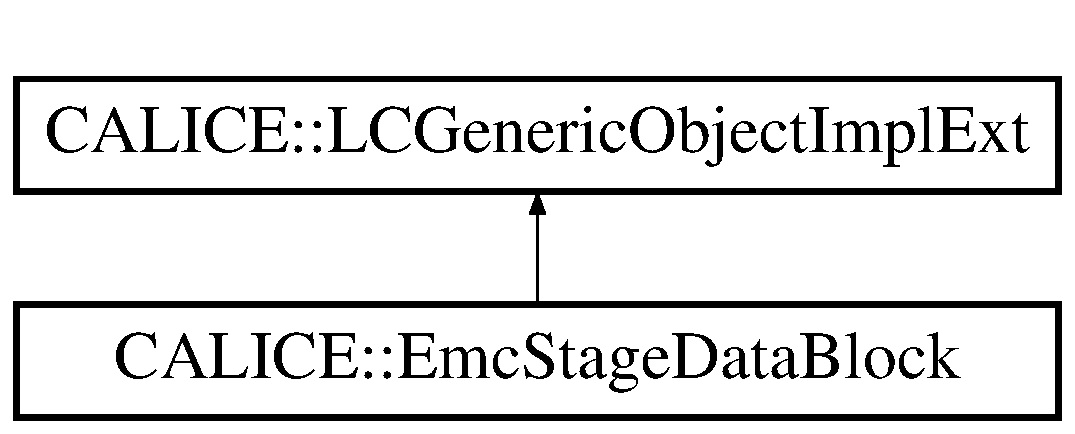
\includegraphics[height=2cm]{classCALICE_1_1EmcStageDataBlock}
\end{center}
\end{figure}
\subsection*{Public Member Functions}
\begin{DoxyCompactItemize}
\item 
{\bf EmcStageDataBlock} ()\label{classCALICE_1_1EmcStageDataBlock_afaee0059f5d693fea74c762e17f789cf}

\begin{DoxyCompactList}\small\item\em Default Constructor. \item\end{DoxyCompactList}\item 
{\bf EmcStageDataBlock} (LCObject $\ast$obj)\label{classCALICE_1_1EmcStageDataBlock_aab94abf8e8f16cee02984b0f07123508}

\begin{DoxyCompactList}\small\item\em 'Copy constructor' needed to interpret LCCollection read from file/database. \item\end{DoxyCompactList}\item 
{\bf EmcStageDataBlock} \& {\bf setHeader} (int header)\label{classCALICE_1_1EmcStageDataBlock_a450b26e7aa41c180d81d248171713181}

\begin{DoxyCompactList}\small\item\em Set the header data. \item\end{DoxyCompactList}\item 
{\bf EmcStageDataBlock} \& {\bf setXYStatus} (int xStatus, int yStatus)\label{classCALICE_1_1EmcStageDataBlock_aced038a7dcb48dda69af993b430cda10}

\begin{DoxyCompactList}\small\item\em Set the x and yStatus data. \item\end{DoxyCompactList}\item 
{\bf EmcStageDataBlock} \& {\bf setXYValues} (int $\ast$xValue, int $\ast$yValue)\label{classCALICE_1_1EmcStageDataBlock_a11886d8d49678205ed77c4cb6066ce95}

\begin{DoxyCompactList}\small\item\em Set the x and y Value data. \item\end{DoxyCompactList}\item 
{\bf EmcStageDataBlock} \& {\bf setCheckSum} (int checksum)\label{classCALICE_1_1EmcStageDataBlock_a85187bcae7309db33c9a9e4db978b888}

\begin{DoxyCompactList}\small\item\em Set the checksum. \item\end{DoxyCompactList}\item 
int {\bf getHeader} ()\label{classCALICE_1_1EmcStageDataBlock_a618d05f308f47206f70251a4839afaed}

\begin{DoxyCompactList}\small\item\em Return the header. \item\end{DoxyCompactList}\item 
bool {\bf getXIndexerStatus} ()\label{classCALICE_1_1EmcStageDataBlock_a1aa86f87b01550f432e76a32ed67fbbb}

\begin{DoxyCompactList}\small\item\em Return the XIndexerStatus. \item\end{DoxyCompactList}\item 
bool {\bf getYIndexerStatus} ()\label{classCALICE_1_1EmcStageDataBlock_aaefa28fb2beb7b52bda42e7a4614d042}

\begin{DoxyCompactList}\small\item\em Return the YIndexerStatus. \item\end{DoxyCompactList}\item 
int {\bf getXStandPosition} ()\label{classCALICE_1_1EmcStageDataBlock_a4b386bbe2e428d64f5edddb3684db89c}

\begin{DoxyCompactList}\small\item\em Return the xStand Position. \item\end{DoxyCompactList}\item 
int {\bf getYStandPosition} ()\label{classCALICE_1_1EmcStageDataBlock_ab82f727e4d2cdf7c519c7ba4534a01e7}

\begin{DoxyCompactList}\small\item\em Return the yStand Position. \item\end{DoxyCompactList}\item 
int {\bf getXBeamPosition} ()\label{classCALICE_1_1EmcStageDataBlock_a6600b388e82b3e6659c6d9b9a68e32a7}

\begin{DoxyCompactList}\small\item\em Return the xBeam Position. \item\end{DoxyCompactList}\item 
int {\bf getYBeamPosition} ()\label{classCALICE_1_1EmcStageDataBlock_a9b1559b6277c4e67c8bec00fa3d1b935}

\begin{DoxyCompactList}\small\item\em Return the yBeam Position. \item\end{DoxyCompactList}\item 
int {\bf getCheckSum} ()\label{classCALICE_1_1EmcStageDataBlock_a476eec95c90336a3566c1a845d3c72d0}

\begin{DoxyCompactList}\small\item\em Return the checksum. \item\end{DoxyCompactList}\item 
void {\bf print} (std::ostream \&os)\label{classCALICE_1_1EmcStageDataBlock_adf909ff47ea9c2d6eeece246a5c78573}

\begin{DoxyCompactList}\small\item\em Convenient print method. \item\end{DoxyCompactList}\item 
const std::string {\bf getTypeName} () const \label{classCALICE_1_1EmcStageDataBlock_abcc5679cda6f9ec1394ca4e89bbba65a}

\begin{DoxyCompactList}\small\item\em Return the type of the class. \item\end{DoxyCompactList}\item 
const std::string {\bf getDataDescription} () const \label{classCALICE_1_1EmcStageDataBlock_a31475ed6c87dece26d94116216e20c32}

\begin{DoxyCompactList}\small\item\em Return a brief description of the data members. \item\end{DoxyCompactList}\end{DoxyCompactItemize}


\subsection{Detailed Description}
Stores information about the Emc stage Here we need to duplicate a lot of code already written by Paul since we cannot top the 'intelligence' which is introduced already there. For the time being we return only the (to my taste) most important values. The others can be added easily if really needed. \begin{DoxySeeAlso}{See also}
\doxyref{ConditionsChangeDelegator}{p.}{classCALICE_1_1ConditionsChangeDelegator} 
\end{DoxySeeAlso}
\begin{DoxyAuthor}{Author}
R. Poeschl LAL (based on the other interface classes)
\end{DoxyAuthor}
\begin{DoxyDate}{Date}
June 2006 
\end{DoxyDate}


Definition at line 42 of file EmcStageDataBlock.hh.

The documentation for this class was generated from the following files:\begin{DoxyCompactItemize}
\item 
EmcStageDataBlock.hh\item 
EmcStageDataBlock.cc\end{DoxyCompactItemize}

\section{CALICE::EncodingStringHelper Class Reference}
\label{classCALICE_1_1EncodingStringHelper}\index{CALICE::EncodingStringHelper@{CALICE::EncodingStringHelper}}


Utility class to get the field description according to an lcio BitField64.  


{\ttfamily \#include $<$EncodingStringHelper.hh$>$}\subsection*{Static Public Member Functions}
\begin{DoxyCompactItemize}
\item 
static std::string {\bf GetFieldDesc} (const std::string FieldName, const unsigned int FieldMask, const unsigned int FieldShift, const unsigned int startbit)
\end{DoxyCompactItemize}


\subsection{Detailed Description}
Utility class to get the field description according to an lcio BitField64. \begin{DoxyAuthor}{Author}
S. Richter (DESY) 
\end{DoxyAuthor}
\begin{DoxyDate}{Date}
March 13 2007 
\end{DoxyDate}


Definition at line 13 of file EncodingStringHelper.hh.

\subsection{Member Function Documentation}
\index{CALICE::EncodingStringHelper@{CALICE::EncodingStringHelper}!GetFieldDesc@{GetFieldDesc}}
\index{GetFieldDesc@{GetFieldDesc}!CALICE::EncodingStringHelper@{CALICE::EncodingStringHelper}}
\subsubsection[{GetFieldDesc}]{\setlength{\rightskip}{0pt plus 5cm}std::string CALICE::EncodingStringHelper::GetFieldDesc (const std::string {\em FieldName}, \/  const unsigned int {\em FieldMask}, \/  const unsigned int {\em FieldShift}, \/  const unsigned int {\em startbit})\hspace{0.3cm}{\ttfamily  [static]}}\label{classCALICE_1_1EncodingStringHelper_acf70b62844698b1cc0fb9e04531d5ba4}

\begin{DoxyParams}{Parameters}
\item[{\em FieldName}]-\/ the identifier of the field, e.g. \char`\"{}module\char`\"{} \item[{\em FieldMask}]-\/ the bitmask which specifies the bits used for this field \item[{\em FieldShift}]-\/ using the shift together with the mask you get field at the lowest bits \item[{\em startbit}]-\/ an overall shift of all fields \end{DoxyParams}


Definition at line 7 of file EncodingStringHelper.cc.

Referenced by CALICE::HcalTileIndex::getEncodingString(), and CALICE::HcalCellIndex::getEncodingString().

The documentation for this class was generated from the following files:\begin{DoxyCompactItemize}
\item 
EncodingStringHelper.hh\item 
EncodingStringHelper.cc\end{DoxyCompactItemize}

\section{CALICE::ErrorBits Class Reference}
\label{classCALICE_1_1ErrorBits}\index{CALICE::ErrorBits@{CALICE::ErrorBits}}


Helper class to query or set the event errors.  


{\ttfamily \#include $<$ErrorBits.hh$>$}\subsection*{Public Types}
\begin{DoxyCompactItemize}
\item 
enum {\bfseries EErrorBits} \{ \par
{\bfseries kNoEventData}, 
{\bfseries kMissingAdcBlock}, 
{\bfseries kMissingVLinkHeader}, 
{\bfseries kInvalidTrigger}, 
\par
{\bfseries kBadConfigData}, 
{\bfseries kWrongTriggerCounter}, 
{\bfseries kCorruptEventRecord}, 
{\bfseries kMissingTriggerRecord}, 
\par
{\bfseries kCorruptAcquisition}, 
{\bfseries kTDCOutOfSynch}, 
{\bfseries kDirtyEvent}, 
{\bfseries kLargeNegativeSignal}, 
\par
{\bfseries kCorruptBmlRecord}, 
{\bfseries kCorruptDifTrigCounter}, 
{\bfseries kNErrorBits}
 \}
\end{DoxyCompactItemize}
\subsection*{Public Member Functions}
\begin{DoxyCompactItemize}
\item 
{\bfseries ErrorBits} (int trigger\_\-bits)\label{classCALICE_1_1ErrorBits_a927b74aac9ca3f891c36c473ff4442dc}

\item 
bool {\bf operator!} () const \label{classCALICE_1_1ErrorBits_ad93c6729233b5798daa61b312fa762ea}

\begin{DoxyCompactList}\small\item\em Return true if NO error was detected. \item\end{DoxyCompactList}\item 
{\bf operator bool} () const \label{classCALICE_1_1ErrorBits_a61ab35bd38f6357c663a5bc3af3e5aa7}

\begin{DoxyCompactList}\small\item\em Return true if an error was detected. \item\end{DoxyCompactList}\item 
bool {\bf noEventData} () const \label{classCALICE_1_1ErrorBits_a375385c62d316d1961fa31180546c8b6}

\begin{DoxyCompactList}\small\item\em Was the event data missing for this event? return true if all ADC blocks were missing;. \item\end{DoxyCompactList}\item 
void {\bf setNoEventData} ()\label{classCALICE_1_1ErrorBits_ab4b06519a8a5108fb722f7e5f67bfe3f}

\begin{DoxyCompactList}\small\item\em Set the missing event data flag. \item\end{DoxyCompactList}\item 
bool {\bf missingADCBlock} () const \label{classCALICE_1_1ErrorBits_a7bf182209fc6806fb29c427378bccc49}

\begin{DoxyCompactList}\small\item\em Is one or more ADC blocks missing? return true if one or more ADC blocks are missing. \item\end{DoxyCompactList}\item 
void {\bf setMissingADCBlock} ()\label{classCALICE_1_1ErrorBits_a3995149a7c9509b200aa39aa199b845d}

\begin{DoxyCompactList}\small\item\em Set the error bit to flag missing ADC blocks. \item\end{DoxyCompactList}\item 
bool {\bf missingVLinkHeader} () const \label{classCALICE_1_1ErrorBits_acdc6a1950dcfb3bd6ae8582b05642aa9}

\begin{DoxyCompactList}\small\item\em Is the VLink Header missing? return true if the VLink header is missing. \item\end{DoxyCompactList}\item 
void {\bf setMissingVLinkHeader} ()\label{classCALICE_1_1ErrorBits_af424a5412ff42f2cb9f17ab903b5d9af}

\begin{DoxyCompactList}\small\item\em Set the error bit to flag missing VLink headers. \item\end{DoxyCompactList}\item 
bool {\bf wrongTriggerCounter} () const 
\begin{DoxyCompactList}\small\item\em Return true if the trigger counter did not change or is not the same for all \char`\"{}valid\char`\"{} front-\/ends. \item\end{DoxyCompactList}\item 
void {\bf setWrongTriggerCounter} ()\label{classCALICE_1_1ErrorBits_a15c07fc0003b77ea84cea8f6f02ca9af}

\begin{DoxyCompactList}\small\item\em Set the error bit to flag errors in the trigger counter field. \item\end{DoxyCompactList}\item 
bool {\bf corruptEventRecord} () const \label{classCALICE_1_1ErrorBits_aefd9055151234a0a9d075985494e3891}

\begin{DoxyCompactList}\small\item\em Return true if the event record of one front-\/end was corrupt. \item\end{DoxyCompactList}\item 
void {\bf setCorruptEventRecord} ()\label{classCALICE_1_1ErrorBits_affd6ab2f3ebe14933e8bf3dd035f68ae}

\begin{DoxyCompactList}\small\item\em Set the error bit to flag events with corrupt event records. \item\end{DoxyCompactList}\item 
bool {\bf invalidTrigger} () const 
\begin{DoxyCompactList}\small\item\em Is the Vlink header missing ?. \item\end{DoxyCompactList}\item 
void {\bf setInvalidTrigger} ()\label{classCALICE_1_1ErrorBits_acd20ea1331d9aea5f77338117c38831a}

\begin{DoxyCompactList}\small\item\em Set the error bit to flag missing VLink headers. \item\end{DoxyCompactList}\item 
bool {\bf badConfigurationData} () const \label{classCALICE_1_1ErrorBits_ab59c0f2e38e8813f64590675ce87ffa5}

\begin{DoxyCompactList}\small\item\em Error in the verification of the Configuration Data. \item\end{DoxyCompactList}\item 
void {\bf setBadConfigurationData} ()\label{classCALICE_1_1ErrorBits_a3c660d52477a79185cd5e7ad3dc78461}

\begin{DoxyCompactList}\small\item\em Set the error bit to flag bad Configuration Data. \item\end{DoxyCompactList}\item 
bool {\bf noTrigger} () const \label{classCALICE_1_1ErrorBits_a7396f0ba339785a399c04b9ce2d6f485}

\begin{DoxyCompactList}\small\item\em No trigger exists for a given event. \item\end{DoxyCompactList}\item 
void {\bf setNoTrigger} ()\label{classCALICE_1_1ErrorBits_afea7c27ccb3a9572c8d130c5996a8455}

\begin{DoxyCompactList}\small\item\em Set the error bit to flag bad Configuration Data. \item\end{DoxyCompactList}\item 
bool {\bf corruptAcquisition} () const 
\begin{DoxyCompactList}\small\item\em The acquisition sequence is screwed up i.e. \item\end{DoxyCompactList}\item 
void {\bf setCorruptAcquisition} ()\label{classCALICE_1_1ErrorBits_a3558273df772aed0bd6df136d60ec2b6}

\begin{DoxyCompactList}\small\item\em Set the error bit to flag a wrong acquistion. \item\end{DoxyCompactList}\item 
bool {\bf tdcOutOfSynch} () const \label{classCALICE_1_1ErrorBits_a0052f24179e97549b33e74e48c509d5c}

\begin{DoxyCompactList}\small\item\em The event number in the TDC does not agree with the the event number as derived from the CrcBoards. \item\end{DoxyCompactList}\item 
void {\bf setTDCOutOfSynch} ()\label{classCALICE_1_1ErrorBits_a78ea112b365a2a78e139e62797975f73}

\begin{DoxyCompactList}\small\item\em Set the error bit to flag suspicious TDC data. \item\end{DoxyCompactList}\item 
bool {\bf corruptBmlRecord} () const \label{classCALICE_1_1ErrorBits_a583406b4227795d92a8df89891e7eb71}

\begin{DoxyCompactList}\small\item\em Return true if the event record of one front-\/end was corrupt. \item\end{DoxyCompactList}\item 
void {\bf setCorruptBmlRecord} ()\label{classCALICE_1_1ErrorBits_a051549408253fec1193735666535fe76}

\begin{DoxyCompactList}\small\item\em Set the error bit to flag events with corrupt event records. \item\end{DoxyCompactList}\item 
bool {\bf largeNegativeSignal} () const 
\begin{DoxyCompactList}\small\item\em The event contained a significant fraction of negative signals. \item\end{DoxyCompactList}\item 
void {\bf setLargeNegativeSignal} ()
\begin{DoxyCompactList}\small\item\em Set this error bit if the event contains a significant fraction of negative signals. \item\end{DoxyCompactList}\item 
bool {\bf dirtyEvent} () const \label{classCALICE_1_1ErrorBits_a7f26f5604b4cff6ed6f9282bda47385a}

\begin{DoxyCompactList}\small\item\em Thers is additional trigger activity close to or at the main word. \item\end{DoxyCompactList}\item 
void {\bf setDirtyEvent} ()\label{classCALICE_1_1ErrorBits_af8303261caeb9a0806fa061c9edb6eff}

\begin{DoxyCompactList}\small\item\em Set this error bit if there is additional trigger activity close to or at the main word. \item\end{DoxyCompactList}\item 
bool {\bf corruptDifTrigCounter} () const \label{classCALICE_1_1ErrorBits_a93415444d09fa1b245de4501b35ce325}

\begin{DoxyCompactList}\small\item\em Return true if one of the dif trigger counters gets out of synch. \item\end{DoxyCompactList}\item 
void {\bf setCorruptDifTrigCounter} ()\label{classCALICE_1_1ErrorBits_ab189195a448fce19a6441366e9ce3337}

\begin{DoxyCompactList}\small\item\em Set the error bit to flag events with corrupt dif counter. \item\end{DoxyCompactList}\item 
bool {\bf isSet} () const \label{classCALICE_1_1ErrorBits_a1e38b12fe5037dd02b26f17cb32da7e8}

\begin{DoxyCompactList}\small\item\em Has an error occurred? \item\end{DoxyCompactList}\item 
int {\bf getBits} () const \label{classCALICE_1_1ErrorBits_a9095dd6bfc5635b4acf1b3075f64896d}

\begin{DoxyCompactList}\small\item\em return the error bits. \item\end{DoxyCompactList}\item 
std::ostream \& {\bf print} (std::ostream \&out) const \label{classCALICE_1_1ErrorBits_a57f38311627524b0a880eee60384a96d}

\begin{DoxyCompactList}\small\item\em print the current errors. \item\end{DoxyCompactList}\end{DoxyCompactItemize}
\subsection*{Static Public Member Functions}
\begin{DoxyCompactItemize}
\item 
static unsigned int {\bf getErrorBit} (const std::string \&name)\label{classCALICE_1_1ErrorBits_aa77e243148d98a950c3a973babea5c4f}

\begin{DoxyCompactList}\small\item\em Translate an error name into a bit. \item\end{DoxyCompactList}\item 
static const char $\ast$ {\bf getErrorName} (unsigned int bit\_\-i)\label{classCALICE_1_1ErrorBits_ae207446de0aca583ea7959531c4043d8}

\begin{DoxyCompactList}\small\item\em Get the name assigned to an error bit. \item\end{DoxyCompactList}\item 
static unsigned int {\bf getErrorBitMask} (const std::vector$<$ std::string $>$ \&error\_\-names)\label{classCALICE_1_1ErrorBits_a19612286cd3ea90c228cd913a22a958a}

\begin{DoxyCompactList}\small\item\em Create a error bit mask from a vector of error names. \item\end{DoxyCompactList}\end{DoxyCompactItemize}
\subsection*{Private Member Functions}
\begin{DoxyCompactItemize}
\item 
bool {\bf getBit} (unsigned int bit) const \label{classCALICE_1_1ErrorBits_a2a8cbd878f868fd75e85710f9af16bbb}

\begin{DoxyCompactList}\small\item\em get an error bit. \item\end{DoxyCompactList}\item 
void {\bf setBit} (unsigned int bit)\label{classCALICE_1_1ErrorBits_a647e5048a691fac67036503fabc7d2d7}

\begin{DoxyCompactList}\small\item\em set an error bit. \item\end{DoxyCompactList}\end{DoxyCompactItemize}
\subsection*{Private Attributes}
\begin{DoxyCompactItemize}
\item 
int {\bf \_\-errorBits}
\begin{DoxyCompactList}\small\item\em The error bits. \item\end{DoxyCompactList}\end{DoxyCompactItemize}
\subsection*{Static Private Attributes}
\begin{DoxyCompactItemize}
\item 
static const char $\ast$ {\bfseries \_\-\_\-name} [kNErrorBits]
\item 
static std::map$<$ std::string, unsigned short $>$ {\bfseries \_\-\_\-nameToBit}\label{classCALICE_1_1ErrorBits_a68e0b7db3f43e82cce09c946571a8323}

\end{DoxyCompactItemize}


\subsection{Detailed Description}
Helper class to query or set the event errors. usage:

\doxyref{ErrorBits}{p.}{classCALICE_1_1ErrorBits} error(((LCEvent $\ast$) evt)-\/$>$getParameters().getIntVal(PAR\_\-ERROR\_\-BITS));

\begin{DoxyAuthor}{Author}
G�tz Gaycken LLR (Ecole Polytechnique) 
\end{DoxyAuthor}
\begin{DoxyDate}{Date}
Apr 2005 
\end{DoxyDate}


Definition at line 21 of file ErrorBits.hh.

\subsection{Member Function Documentation}
\index{CALICE::ErrorBits@{CALICE::ErrorBits}!corruptAcquisition@{corruptAcquisition}}
\index{corruptAcquisition@{corruptAcquisition}!CALICE::ErrorBits@{CALICE::ErrorBits}}
\subsubsection[{corruptAcquisition}]{\setlength{\rightskip}{0pt plus 5cm}bool CALICE::ErrorBits::corruptAcquisition () const\hspace{0.3cm}{\ttfamily  [inline]}}\label{classCALICE_1_1ErrorBits_a1ae3ecf26cbb5f59fa0f5bc99fca5bdd}


The acquisition sequence is screwed up i.e. unequal numbers of event and trigger records 

Definition at line 134 of file ErrorBits.hh.

References getBit().\index{CALICE::ErrorBits@{CALICE::ErrorBits}!invalidTrigger@{invalidTrigger}}
\index{invalidTrigger@{invalidTrigger}!CALICE::ErrorBits@{CALICE::ErrorBits}}
\subsubsection[{invalidTrigger}]{\setlength{\rightskip}{0pt plus 5cm}bool CALICE::ErrorBits::invalidTrigger () const\hspace{0.3cm}{\ttfamily  [inline]}}\label{classCALICE_1_1ErrorBits_af0c5d30fbfe9bda5d36a5e1ef90ec346}


Is the Vlink header missing ?. return true if the VLink header is missing. 

Definition at line 110 of file ErrorBits.hh.

References getBit().\index{CALICE::ErrorBits@{CALICE::ErrorBits}!largeNegativeSignal@{largeNegativeSignal}}
\index{largeNegativeSignal@{largeNegativeSignal}!CALICE::ErrorBits@{CALICE::ErrorBits}}
\subsubsection[{largeNegativeSignal}]{\setlength{\rightskip}{0pt plus 5cm}bool CALICE::ErrorBits::largeNegativeSignal () const\hspace{0.3cm}{\ttfamily  [inline]}}\label{classCALICE_1_1ErrorBits_ad92789bf9a35f690109baf8c5eef5e60}


The event contained a significant fraction of negative signals. This may indicate pedestal drift, overlapping events, ... 

Definition at line 161 of file ErrorBits.hh.

References getBit().\index{CALICE::ErrorBits@{CALICE::ErrorBits}!setLargeNegativeSignal@{setLargeNegativeSignal}}
\index{setLargeNegativeSignal@{setLargeNegativeSignal}!CALICE::ErrorBits@{CALICE::ErrorBits}}
\subsubsection[{setLargeNegativeSignal}]{\setlength{\rightskip}{0pt plus 5cm}void CALICE::ErrorBits::setLargeNegativeSignal ()\hspace{0.3cm}{\ttfamily  [inline]}}\label{classCALICE_1_1ErrorBits_a60ac8277f0a3317e4f03db73edd67683}


Set this error bit if the event contains a significant fraction of negative signals. This may indicate pedestal drift, overlapping events, ... 

Definition at line 166 of file ErrorBits.hh.

References setBit().\index{CALICE::ErrorBits@{CALICE::ErrorBits}!wrongTriggerCounter@{wrongTriggerCounter}}
\index{wrongTriggerCounter@{wrongTriggerCounter}!CALICE::ErrorBits@{CALICE::ErrorBits}}
\subsubsection[{wrongTriggerCounter}]{\setlength{\rightskip}{0pt plus 5cm}bool CALICE::ErrorBits::wrongTriggerCounter () const\hspace{0.3cm}{\ttfamily  [inline]}}\label{classCALICE_1_1ErrorBits_ae34f2f123e83861911656f112e32e5fe}


Return true if the trigger counter did not change or is not the same for all \char`\"{}valid\char`\"{} front-\/ends. Front-\/ends with missing front-\/end data are not considered also not connected front-\/ends. 

Definition at line 92 of file ErrorBits.hh.

References getBit().

\subsection{Field Documentation}
\index{CALICE::ErrorBits@{CALICE::ErrorBits}!\_\-\_\-name@{\_\-\_\-name}}
\index{\_\-\_\-name@{\_\-\_\-name}!CALICE::ErrorBits@{CALICE::ErrorBits}}
\subsubsection[{\_\-\_\-name}]{\setlength{\rightskip}{0pt plus 5cm}const char $\ast$ CALICE::ErrorBits::\_\-\_\-name\hspace{0.3cm}{\ttfamily  [static, private]}}\label{classCALICE_1_1ErrorBits_a6bd32c898b1541fd337f7ba89719d622}
{\bfseries Initial value:}
\begin{DoxyCode}
{
  "NoEventData",
  "MissingAdcBlock", 
  "MissingVLinkHeader",
  "InvalidTrigger", 
  "BadConfigData", 
  "WrongTriggerCounter",
  "CorruptEventRecord",
  "MissingTriggerRecord", 
  "CorruptAcquisition",
  "TDCOutOfSynch",
  "DirtyEvent",
  "LargeNegativeSignal",
  "CorruptBmlRecord",
  "CorruptDifTriggerCounter"
}
\end{DoxyCode}


Definition at line 231 of file ErrorBits.hh.\index{CALICE::ErrorBits@{CALICE::ErrorBits}!\_\-errorBits@{\_\-errorBits}}
\index{\_\-errorBits@{\_\-errorBits}!CALICE::ErrorBits@{CALICE::ErrorBits}}
\subsubsection[{\_\-errorBits}]{\setlength{\rightskip}{0pt plus 5cm}int {\bf CALICE::ErrorBits::\_\-errorBits}\hspace{0.3cm}{\ttfamily  [private]}}\label{classCALICE_1_1ErrorBits_a58333445921ccb3bcb89b637037257e9}


The error bits. If non zero an error has occurred. 

Definition at line 227 of file ErrorBits.hh.

Referenced by getBit(), getBits(), isSet(), operator bool(), operator!(), print(), and setBit().

The documentation for this class was generated from the following files:\begin{DoxyCompactItemize}
\item 
ErrorBits.hh\item 
ErrorBits.cc\end{DoxyCompactItemize}

\section{CALICE::EUDAQBlock Class Reference}
\label{classCALICE_1_1EUDAQBlock}\index{CALICE::EUDAQBlock@{CALICE::EUDAQBlock}}


Class for the SLCIO EUDAQ Data as acquired by the EUDAQ system.  


{\ttfamily \#include $<$EUDAQBlock.hh$>$}\subsection*{Public Member Functions}
\begin{DoxyCompactItemize}
\item 
{\bf EUDAQBlock} (int CycleNr, int BunchXID, int ChipID, int EvtNr, int Channel, int TDC, int ADC, int HitBit, int GainBit)\label{classCALICE_1_1EUDAQBlock_a2576c4ead40588d8ea075d9629926ce3}

\begin{DoxyCompactList}\small\item\em Convenient c'tor. \item\end{DoxyCompactList}\item 
{\bf EUDAQBlock} (LCObject $\ast$obj)\label{classCALICE_1_1EUDAQBlock_adf2c1a0b660a881f637ae260033b2068}

\begin{DoxyCompactList}\small\item\em 'Copy constructor' needed to interpret LCCollection read from file/database. \item\end{DoxyCompactList}\item 
virtual {\bf $\sim$EUDAQBlock} ()\label{classCALICE_1_1EUDAQBlock_ac009640c79883d5b236ffa1f01a4da08}

\begin{DoxyCompactList}\small\item\em Important for memory handling. \item\end{DoxyCompactList}\item 
int {\bf GetCycleNr} () const \label{classCALICE_1_1EUDAQBlock_a7267f8e75e5ee64c2b558a1cb58b5370}

\begin{DoxyCompactList}\small\item\em get the CycleNr. \item\end{DoxyCompactList}\item 
int {\bf GetBunchXID} () const \label{classCALICE_1_1EUDAQBlock_a9e868629e66c71f4a5086ee4515d75a6}

\begin{DoxyCompactList}\small\item\em get the BunchXID. \item\end{DoxyCompactList}\item 
int {\bf GetChipID} () const \label{classCALICE_1_1EUDAQBlock_a29e7cb6cea36a5726c185af80f602a04}

\begin{DoxyCompactList}\small\item\em get the ChipID. \item\end{DoxyCompactList}\item 
int {\bf GetEvtNr} () const \label{classCALICE_1_1EUDAQBlock_a274bfd6d90f473f1875fd2045268e27f}

\begin{DoxyCompactList}\small\item\em get the EvtNr. \item\end{DoxyCompactList}\item 
int {\bf GetChannel} () const \label{classCALICE_1_1EUDAQBlock_a5665cd40d1deb96c634a7e131be981a8}

\begin{DoxyCompactList}\small\item\em get the Channel. \item\end{DoxyCompactList}\item 
int {\bf GetTDC} () const \label{classCALICE_1_1EUDAQBlock_a66a6c244efdc2357b15350e778f98e56}

\begin{DoxyCompactList}\small\item\em get the TDC. \item\end{DoxyCompactList}\item 
int {\bf GetADC} () const \label{classCALICE_1_1EUDAQBlock_ac6ad7fd2adcc72ed2aa861eac4d89a0d}

\begin{DoxyCompactList}\small\item\em get the ADC. \item\end{DoxyCompactList}\item 
int {\bf GetHitBit} () const \label{classCALICE_1_1EUDAQBlock_a42be25f91cc050d64bba79ff4718b5c4}

\begin{DoxyCompactList}\small\item\em get the HitBit. \item\end{DoxyCompactList}\item 
int {\bf GetGainBit} () const \label{classCALICE_1_1EUDAQBlock_ac2573362003677a183343529bc63d74c}

\begin{DoxyCompactList}\small\item\em get the GainBit. \item\end{DoxyCompactList}\item 
void {\bf print} (std::ostream \&os, int)\label{classCALICE_1_1EUDAQBlock_a4f65b14367aa1123dd7a8a74e5d24ee1}

\begin{DoxyCompactList}\small\item\em Convenient print method. \item\end{DoxyCompactList}\item 
const std::string {\bf getTypeName} () const \label{classCALICE_1_1EUDAQBlock_aea8613f7fc6cbb4bcbc0294a020d3eca}

\begin{DoxyCompactList}\small\item\em Return the type of the class. \item\end{DoxyCompactList}\item 
const std::string {\bf getDataDescription} () const \label{classCALICE_1_1EUDAQBlock_a48d80a041501c9eaada74c500d78074c}

\begin{DoxyCompactList}\small\item\em Return a brief description of the data members. \item\end{DoxyCompactList}\end{DoxyCompactItemize}


\subsection{Detailed Description}
Class for the SLCIO EUDAQ Data as acquired by the EUDAQ system. \begin{DoxyAuthor}{Author}
A. Irles, based on the \doxyref{LabviewBlock2}{p.}{classCALICE_1_1LabviewBlock2} writen by S. Lu DESY Hamburg 
\end{DoxyAuthor}
\begin{DoxyDate}{Date}
May 20 2015 Created for 2015 testbeams EUDAQ data format. 
\end{DoxyDate}


Definition at line 23 of file EUDAQBlock.hh.

The documentation for this class was generated from the following file:\begin{DoxyCompactItemize}
\item 
EUDAQBlock.hh\end{DoxyCompactItemize}

\section{CALICE::EUDAQTempSensorBlock Class Reference}
\label{classCALICE_1_1EUDAQTempSensorBlock}\index{CALICE::EUDAQTempSensorBlock@{CALICE::EUDAQTempSensorBlock}}


Class for the temperature sensor data as acquired by the AHCAL EUDAQ.  


{\ttfamily \#include $<$EUDAQTempSensorBlock.hh$>$}\subsection*{Public Member Functions}
\begin{DoxyCompactItemize}
\item 
{\bf EUDAQTempSensorBlock} (int LDANumber, int PortNumber, int T1, int T2, int T3, int T4, int T5, int T6, int TDIF, int TPWR)\label{classCALICE_1_1EUDAQTempSensorBlock_ae02d2597a925e3e7fd290a0b31d685c3}

\begin{DoxyCompactList}\small\item\em Convenient c'tor. \item\end{DoxyCompactList}\item 
{\bf EUDAQTempSensorBlock} (LCObject $\ast$obj)\label{classCALICE_1_1EUDAQTempSensorBlock_ac20c9533a2640ee57f741cfca85937eb}

\begin{DoxyCompactList}\small\item\em 'Copy constructor' needed to interpret LCCollection read from file/database. \item\end{DoxyCompactList}\item 
virtual {\bf $\sim$EUDAQTempSensorBlock} ()\label{classCALICE_1_1EUDAQTempSensorBlock_a482b674c4674680f57ad441d32d3e7f6}

\begin{DoxyCompactList}\small\item\em Important for memory handling. \item\end{DoxyCompactList}\item 
int {\bfseries GetLDANumber} () const \label{classCALICE_1_1EUDAQTempSensorBlock_ae2f5861ac123e152117d8086d260ed28}

\item 
int {\bfseries GetPortNumber} () const \label{classCALICE_1_1EUDAQTempSensorBlock_aa85c8473e68609696ef73732ce2e1c73}

\item 
int {\bfseries GetT1} () const \label{classCALICE_1_1EUDAQTempSensorBlock_a05f7d3cd2f61b94b7b355dad9ed04e71}

\item 
int {\bfseries GetT2} () const \label{classCALICE_1_1EUDAQTempSensorBlock_a57fceddca009de039005ae35728279bf}

\item 
int {\bfseries GetT3} () const \label{classCALICE_1_1EUDAQTempSensorBlock_abfa60426a963bcd31243be0e472451bd}

\item 
int {\bfseries GetT4} () const \label{classCALICE_1_1EUDAQTempSensorBlock_a02a094c6b095e4aa1a813ba6027b039b}

\item 
int {\bfseries GetT5} () const \label{classCALICE_1_1EUDAQTempSensorBlock_a7dcee9102c3faddf788cb26584bd991f}

\item 
int {\bfseries GetT6} () const \label{classCALICE_1_1EUDAQTempSensorBlock_a8dc023707cd85d0617ac89f9ccd04f91}

\item 
int {\bfseries GetTDIF} () const \label{classCALICE_1_1EUDAQTempSensorBlock_a84eecef47e27057ca1a52c2a771f65ec}

\item 
int {\bfseries GetTPWR} () const \label{classCALICE_1_1EUDAQTempSensorBlock_a5f8f3e5ed6e1dafbd2bd2e5a6c571ded}

\item 
void {\bfseries print} (std::ostream \&os, int)\label{classCALICE_1_1EUDAQTempSensorBlock_a573889f528e77c39321d3042d8715301}

\item 
const std::string {\bf getTypeName} () const \label{classCALICE_1_1EUDAQTempSensorBlock_aaf80776bd59b87c45ef15e10316142c4}

\begin{DoxyCompactList}\small\item\em Return the type of the class. \item\end{DoxyCompactList}\item 
const std::string {\bf getDataDescription} () const \label{classCALICE_1_1EUDAQTempSensorBlock_a63392b2373970e5d7d4854f5027a96ec}

\begin{DoxyCompactList}\small\item\em Return a brief description of the data members. \item\end{DoxyCompactList}\end{DoxyCompactItemize}


\subsection{Detailed Description}
Class for the temperature sensor data as acquired by the AHCAL EUDAQ. The class reflects that the data are received in the EUDAQ \begin{DoxyAuthor}{Author}
A. Irles DESY Hamburg, based on \doxyref{TempSensorBlock}{p.}{classCALICE_1_1TempSensorBlock} by S. Lu (date Dec 17 2012) 
\end{DoxyAuthor}
\begin{DoxyDate}{Date}
25june 2015 
\end{DoxyDate}


Definition at line 23 of file EUDAQTempSensorBlock.hh.

The documentation for this class was generated from the following file:\begin{DoxyCompactItemize}
\item 
EUDAQTempSensorBlock.hh\end{DoxyCompactItemize}

\section{CALICE::EventHeader Class Reference}
\label{classCALICE_1_1EventHeader}\index{CALICE::EventHeader@{CALICE::EventHeader}}


Class to store event header info, i.e.  


{\ttfamily \#include $<$EventHeader.hh$>$}Inheritance diagram for CALICE::EventHeader::\begin{figure}[H]
\begin{center}
\leavevmode
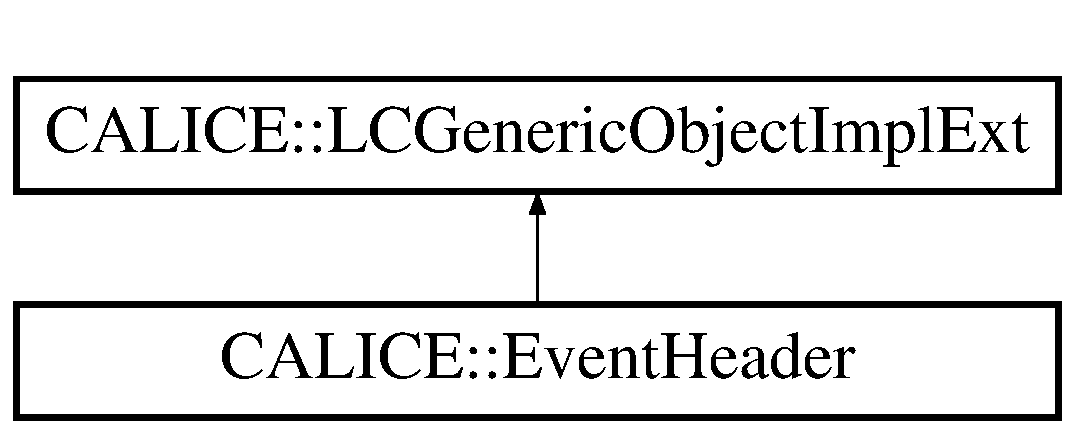
\includegraphics[height=2cm]{classCALICE_1_1EventHeader}
\end{center}
\end{figure}
\subsection*{Public Member Functions}
\begin{DoxyCompactItemize}
\item 
{\bf EventHeader} (int eventNumberInRun, int eventNumberInConfiguration, int eventNumberInAcquisition)\label{classCALICE_1_1EventHeader_a61ce4e0faf985f2d70f92c314eb3033a}

\begin{DoxyCompactList}\small\item\em The costructor. \item\end{DoxyCompactList}\item 
{\bf EventHeader} (LCObject $\ast$obj)\label{classCALICE_1_1EventHeader_a211f090b7c628659f5ea559fde21d95b}

\begin{DoxyCompactList}\small\item\em A copy constructor. \item\end{DoxyCompactList}\item 
virtual {\bf $\sim$EventHeader} ()\label{classCALICE_1_1EventHeader_a2e907c74e6642601f41270e5c8d88c17}

\begin{DoxyCompactList}\small\item\em The destructor. \item\end{DoxyCompactList}\item 
void {\bf setEventNumberInRun} (int evtnumberrun)\label{classCALICE_1_1EventHeader_ab962056e1ab5c7f89184c484b495955e}

\begin{DoxyCompactList}\small\item\em sets the event number in run \item\end{DoxyCompactList}\item 
int {\bf getEventNumberInRun} ()\label{classCALICE_1_1EventHeader_a8f50d11349a3b8d497762ac1cae27d44}

\begin{DoxyCompactList}\small\item\em returns the event number in run \item\end{DoxyCompactList}\item 
void {\bf setEventNumberInConfiguration} (int evtnumberconfig)\label{classCALICE_1_1EventHeader_a6c40f09937e882ab0f178eee8453ad03}

\begin{DoxyCompactList}\small\item\em set the event number in configuration \item\end{DoxyCompactList}\item 
int {\bf getEventNumberInConfiguration} ()\label{classCALICE_1_1EventHeader_ac0d6b7781caddb323548dba760c2cd21}

\begin{DoxyCompactList}\small\item\em returns the event number in configuration \item\end{DoxyCompactList}\item 
void {\bf setEventNumberInAcquisition} (int evtnumberacq)
\begin{DoxyCompactList}\small\item\em returns the event number in spill \item\end{DoxyCompactList}\item 
int {\bf getEventNumberInAcquisition} ()\label{classCALICE_1_1EventHeader_aeb2022e92de4b7cc8a28912ccdd52f73}

\begin{DoxyCompactList}\small\item\em returns the event number in Acquisition \item\end{DoxyCompactList}\item 
const std::string {\bf getTypeName} () const \label{classCALICE_1_1EventHeader_a2db92906b475b2c6409c24535a00d7a6}

\begin{DoxyCompactList}\small\item\em returns the the type name \item\end{DoxyCompactList}\item 
const std::string {\bf getDataDescription} () const \label{classCALICE_1_1EventHeader_a52adc9cbf4000c04b5431406f8df1d83}

\begin{DoxyCompactList}\small\item\em returns a brief description of the data stored \item\end{DoxyCompactList}\item 
std::ostream \& {\bf print} (std::ostream \&ostrm)\label{classCALICE_1_1EventHeader_a1067ef9c5904eb8aa9f1438136c1b5de}

\begin{DoxyCompactList}\small\item\em dumps data content \item\end{DoxyCompactList}\end{DoxyCompactItemize}


\subsection{Detailed Description}
Class to store event header info, i.e. event\# in run, event\# in configuration, event\# in spill

\begin{DoxyAuthor}{Author}
G.Mavromanolakis 
\end{DoxyAuthor}
\begin{DoxyDate}{Date}
8 Jun 2005 
\end{DoxyDate}


Definition at line 37 of file EventHeader.hh.

\subsection{Member Function Documentation}
\index{CALICE::EventHeader@{CALICE::EventHeader}!setEventNumberInAcquisition@{setEventNumberInAcquisition}}
\index{setEventNumberInAcquisition@{setEventNumberInAcquisition}!CALICE::EventHeader@{CALICE::EventHeader}}
\subsubsection[{setEventNumberInAcquisition}]{\setlength{\rightskip}{0pt plus 5cm}void CALICE::EventHeader::setEventNumberInAcquisition (int {\em evtnumberacq})\hspace{0.3cm}{\ttfamily  [inline]}}\label{classCALICE_1_1EventHeader_abb3fb1c88ad338d9bceba1801f344acd}


returns the event number in spill sets the event number in Acquisition 

Definition at line 107 of file EventHeader.hh.

References CALICE::LCGenericObjectImplExt::obj().

Referenced by EventHeader().

The documentation for this class was generated from the following file:\begin{DoxyCompactItemize}
\item 
EventHeader.hh\end{DoxyCompactItemize}

\section{EventStat\_\-t Class Reference}
\label{classEventStat__t}\index{EventStat\_\-t@{EventStat\_\-t}}


Statistics about event data record errors.  


{\ttfamily \#include $<$EventStatList\_\-t.hh$>$}Inheritance diagram for EventStat\_\-t::\begin{figure}[H]
\begin{center}
\leavevmode
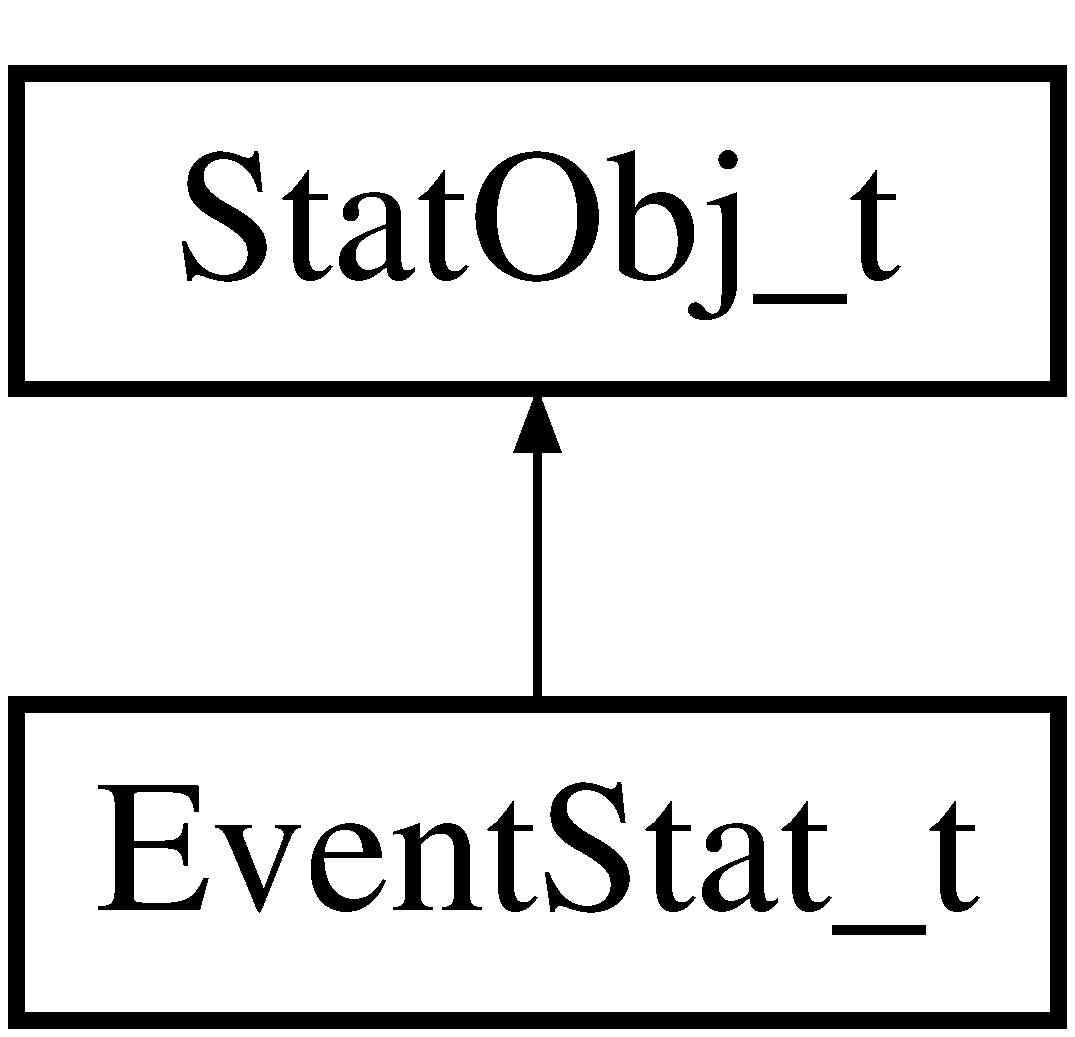
\includegraphics[height=2cm]{classEventStat__t}
\end{center}
\end{figure}
\subsection*{Public Member Functions}
\begin{DoxyCompactItemize}
\item 
void {\bf finish} ()\label{classEventStat__t_a3de34c1b75654309a34e3c59baaf3e3c}

\begin{DoxyCompactList}\small\item\em does nothing. \item\end{DoxyCompactList}\item 
void {\bf printTableHeader} (std::ostream \&out) const \label{classEventStat__t_a04a45113ff065d22de59ed2ead6d773d}

\begin{DoxyCompactList}\small\item\em Print the table header. \item\end{DoxyCompactList}\item 
void {\bf print} (std::ostream \&out)
\begin{DoxyCompactList}\small\item\em Print the statistics of one object (one table row). \item\end{DoxyCompactList}\item 
bool {\bf hasInfo} () const 
\begin{DoxyCompactList}\small\item\em Return true if at least one error was detected for the corresponding front-\/end. \item\end{DoxyCompactList}\item 
void {\bf sameEvent} ()\label{classEventStat__t_ab748cfcf7a8c6adf7704990d45f4cd32}

\begin{DoxyCompactList}\small\item\em Notify that the same event was read out twice. \item\end{DoxyCompactList}\item 
void {\bf corruptRecord} ()\label{classEventStat__t_a06b8038060c09957b59d9559c59e5e69}

\begin{DoxyCompactList}\small\item\em Notify that the record is corrupt. \item\end{DoxyCompactList}\item 
void {\bf triggerCounterMismatch} ()
\begin{DoxyCompactList}\small\item\em Notify about a trigger counter mismitch wrt. \item\end{DoxyCompactList}\item 
void {\bf slotTriggerCounterMismatch} ()
\begin{DoxyCompactList}\small\item\em Notify about a trigger counter mismitch wrt. \item\end{DoxyCompactList}\item 
void {\bf noFeData} ()
\begin{DoxyCompactList}\small\item\em Notify missing front-\/end event data. \item\end{DoxyCompactList}\item 
void {\bf feData} ()
\begin{DoxyCompactList}\small\item\em Notify about available front-\/end event data. \item\end{DoxyCompactList}\item 
void {\bf setBadVLinkHeader} ()\label{classEventStat__t_a20178de3ef951d0f652c5e09d4b4f8b3}

\begin{DoxyCompactList}\small\item\em Notify bad Vlink Headers according to Pauls verify function. \item\end{DoxyCompactList}\item 
void {\bf setDestroyedCrcVLinkRecords} ()
\begin{DoxyCompactList}\small\item\em Notify completetly corrupt ADC records (e.g. \item\end{DoxyCompactList}\item 
unsigned int {\bf refreshErrors} () const \label{classEventStat__t_a40c058f85ad9be40b3dc392c38b3ff91}

\begin{DoxyCompactList}\small\item\em The total number of events for which the previous event was read again instead of a new one. \item\end{DoxyCompactList}\item 
unsigned int {\bf recordErrors} () const \label{classEventStat__t_a3a7d8aee8e1bf39263d8c3a10d197953}

\begin{DoxyCompactList}\small\item\em The total number of events for which the event data record was corrupt. \item\end{DoxyCompactList}\item 
unsigned int {\bf triggerCounterErrors} () const \label{classEventStat__t_a9b63de0930de74c3827ed75df652c2e6}

\begin{DoxyCompactList}\small\item\em The total number of events for which the trigger counter did not match the one of the previous front-\/end. \item\end{DoxyCompactList}\item 
unsigned int {\bf slotTriggerCounterErrors} () const \label{classEventStat__t_af44aefda07aef191437386190d0998be}

\begin{DoxyCompactList}\small\item\em The total number of events for which the trigger counter did not match the one of the previous slot. \item\end{DoxyCompactList}\item 
unsigned int {\bf eventsWithoutFeData} () const \label{classEventStat__t_a95a0af550b916e6e2680129805f6c19b}

\begin{DoxyCompactList}\small\item\em The total number of events for which the front-\/end event data was missing. \item\end{DoxyCompactList}\item 
unsigned int {\bf badVLinkHeaders} ()\label{classEventStat__t_a5909605a8f59205ca411ebf168dd586e}

\begin{DoxyCompactList}\small\item\em Return the number of bad VLink Headers. \item\end{DoxyCompactList}\item 
unsigned int {\bf destroyedCrcVLinkRecords} ()\label{classEventStat__t_a1346627746f75d2b4705676d9bacc253}

\begin{DoxyCompactList}\small\item\em Return the number of destroyed CrcVLinkData. \item\end{DoxyCompactList}\item 
unsigned int {\bf error} () const \label{classEventStat__t_ae4ef03c2850a29ba8352eb390339d1f3}

\begin{DoxyCompactList}\small\item\em The total number of errors. \item\end{DoxyCompactList}\end{DoxyCompactItemize}
\subsection*{Private Attributes}
\begin{DoxyCompactItemize}
\item 
unsigned int {\bfseries \_\-sameEvent}\label{classEventStat__t_af47df69fa27240a369ea766830a0115f}

\item 
unsigned int {\bfseries \_\-corruptRecord}\label{classEventStat__t_a741c0870676516c066bee748da17946f}

\item 
unsigned int {\bfseries \_\-triggerCounterMismatch}\label{classEventStat__t_ad981f571d83750d02892285c752138b6}

\item 
unsigned int {\bfseries \_\-slotTriggerCounterMismatch}\label{classEventStat__t_a317b5d148ff956fb911d567054179a8a}

\item 
unsigned int {\bfseries \_\-missingFeData}\label{classEventStat__t_a8fd34eec37ae8aff59e361685272d217}

\item 
unsigned int {\bfseries \_\-nFeData}\label{classEventStat__t_a3cbd7d4a994750f7b5bd681813dca063}

\item 
unsigned int {\bf \_\-nBadHeader}\label{classEventStat__t_a994ba3454f481e8a05e2a7a1dad0f912}

\begin{DoxyCompactList}\small\item\em variables counting missing header info \item\end{DoxyCompactList}\item 
unsigned int {\bfseries \_\-nDesCrcVLink}\label{classEventStat__t_a09b8fe6143725978872e3a4746925f9b}

\end{DoxyCompactItemize}


\subsection{Detailed Description}
Statistics about event data record errors. The object is meant to be used together with \doxyref{FeStatList\_\-t}{p.}{classFeStatList__t}. This object collects statistics about bad event data records The following errors are counted: the same event was read out twice; the trigger counter does not match the trigger counter of another Crc Board; the record is corrupt. \begin{DoxyAuthor}{Author}
Goetz Gaycken, LLR -\/ Ecole polytechnique 
\end{DoxyAuthor}
\begin{DoxyDate}{Date}
feb, 2006 
\end{DoxyDate}


Definition at line 16 of file EventStatList\_\-t.hh.

\subsection{Member Function Documentation}
\index{EventStat\_\-t@{EventStat\_\-t}!feData@{feData}}
\index{feData@{feData}!EventStat_t@{EventStat\_\-t}}
\subsubsection[{feData}]{\setlength{\rightskip}{0pt plus 5cm}void EventStat\_\-t::feData ()\hspace{0.3cm}{\ttfamily  [inline]}}\label{classEventStat__t_a43220a2eae852d1f48b0a79fd0ea9a9a}


Notify about available front-\/end event data. If front-\/end data is missing always than it is not an error. 

Definition at line 61 of file EventStatList\_\-t.hh.\index{EventStat\_\-t@{EventStat\_\-t}!hasInfo@{hasInfo}}
\index{hasInfo@{hasInfo}!EventStat_t@{EventStat\_\-t}}
\subsubsection[{hasInfo}]{\setlength{\rightskip}{0pt plus 5cm}bool EventStat\_\-t::hasInfo () const\hspace{0.3cm}{\ttfamily  [inline, virtual]}}\label{classEventStat__t_aa34365be6467dd0a2567513a3368c1f2}


Return true if at least one error was detected for the corresponding front-\/end. 

Implements {\bf StatObj\_\-t} \doxyref{}{p.}{classStatObj__t_a4eb553db0bda3666cab1c390092841a1}.

Definition at line 35 of file EventStatList\_\-t.hh.

References error().\index{EventStat\_\-t@{EventStat\_\-t}!noFeData@{noFeData}}
\index{noFeData@{noFeData}!EventStat_t@{EventStat\_\-t}}
\subsubsection[{noFeData}]{\setlength{\rightskip}{0pt plus 5cm}void EventStat\_\-t::noFeData ()\hspace{0.3cm}{\ttfamily  [inline]}}\label{classEventStat__t_a97f8a0c024af090610b7b2015d0ce60f}


Notify missing front-\/end event data. The front-\/end event data is needed to identify corrupt records and find trigger counter mismatches. 

Definition at line 56 of file EventStatList\_\-t.hh.\index{EventStat\_\-t@{EventStat\_\-t}!print@{print}}
\index{print@{print}!EventStat_t@{EventStat\_\-t}}
\subsubsection[{print}]{\setlength{\rightskip}{0pt plus 5cm}void EventStat\_\-t::print (std::ostream \& {\em out})\hspace{0.3cm}{\ttfamily  [virtual]}}\label{classEventStat__t_a518be219247fbd9108e6d186796d9b64}


Print the statistics of one object (one table row). 

Implements {\bf StatObj\_\-t} \doxyref{}{p.}{classStatObj__t_a2763586ba61eb2c37f076e266b0a331e}.

Definition at line 16 of file EventStatList\_\-t.cc.

References badVLinkHeaders(), destroyedCrcVLinkRecords(), eventsWithoutFeData(), recordErrors(), refreshErrors(), slotTriggerCounterErrors(), and triggerCounterErrors().\index{EventStat\_\-t@{EventStat\_\-t}!setDestroyedCrcVLinkRecords@{setDestroyedCrcVLinkRecords}}
\index{setDestroyedCrcVLinkRecords@{setDestroyedCrcVLinkRecords}!EventStat_t@{EventStat\_\-t}}
\subsubsection[{setDestroyedCrcVLinkRecords}]{\setlength{\rightskip}{0pt plus 5cm}void EventStat\_\-t::setDestroyedCrcVLinkRecords ()\hspace{0.3cm}{\ttfamily  [inline]}}\label{classEventStat__t_affecaa835813d871d69af374935c4c5e}


Notify completetly corrupt ADC records (e.g. at beginning of config 

Definition at line 70 of file EventStatList\_\-t.hh.\index{EventStat\_\-t@{EventStat\_\-t}!slotTriggerCounterMismatch@{slotTriggerCounterMismatch}}
\index{slotTriggerCounterMismatch@{slotTriggerCounterMismatch}!EventStat_t@{EventStat\_\-t}}
\subsubsection[{slotTriggerCounterMismatch}]{\setlength{\rightskip}{0pt plus 5cm}void EventStat\_\-t::slotTriggerCounterMismatch ()\hspace{0.3cm}{\ttfamily  [inline]}}\label{classEventStat__t_a15423117d12b710fe046d2c7474b68cf}


Notify about a trigger counter mismitch wrt. to the previous Crc board. 

Definition at line 51 of file EventStatList\_\-t.hh.\index{EventStat\_\-t@{EventStat\_\-t}!triggerCounterMismatch@{triggerCounterMismatch}}
\index{triggerCounterMismatch@{triggerCounterMismatch}!EventStat_t@{EventStat\_\-t}}
\subsubsection[{triggerCounterMismatch}]{\setlength{\rightskip}{0pt plus 5cm}void EventStat\_\-t::triggerCounterMismatch ()\hspace{0.3cm}{\ttfamily  [inline]}}\label{classEventStat__t_ab2b08c993ac66fed880d26a01e3fbda7}


Notify about a trigger counter mismitch wrt. to the last \char`\"{}good\char`\"{} front-\/end. 

Definition at line 47 of file EventStatList\_\-t.hh.

The documentation for this class was generated from the following files:\begin{DoxyCompactItemize}
\item 
EventStatList\_\-t.hh\item 
EventStatList\_\-t.cc\end{DoxyCompactItemize}

\section{CALICE::ExperimentalSetup Class Reference}
\label{classCALICE_1_1ExperimentalSetup}\index{CALICE::ExperimentalSetup@{CALICE::ExperimentalSetup}}


Define the experimental setup: beam energy, position, angle and detector position, angle.  


{\ttfamily \#include $<$ExperimentalSetup.hh$>$}\subsection*{Public Types}
\begin{DoxyCompactItemize}
\item 
enum {\bfseries EBeamType} \{ \par
{\bfseries kElectronBeam}, 
{\bfseries kMuonBeam}, 
{\bfseries kPionBeam}, 
{\bfseries kProtonBeam}, 
\par
{\bfseries kCosmics}, 
{\bfseries kUnknown}, 
{\bfseries kMixed}, 
{\bfseries kPionElectronBeam}, 
\par
{\bfseries kPionProtonBeam}, 
{\bfseries kCalibrationPulse}, 
{\bfseries kNoise}, 
{\bfseries kNBeamTypes}
 \}
\end{DoxyCompactItemize}
\subsection*{Public Member Functions}
\begin{DoxyCompactItemize}
\item 
{\bf ExperimentalSetup} (LCObject $\ast$obj)\label{classCALICE_1_1ExperimentalSetup_a88f1b7e3e0bcfa5ef4a7941aa73e9695}

\begin{DoxyCompactList}\small\item\em 'Copy constructor' needed to interpret LCCollection read from file/database. \item\end{DoxyCompactList}\item 
{\bf ExperimentalSetup} \& {\bf setBeamType} (EBeamType beam\_\-type)\label{classCALICE_1_1ExperimentalSetup_a20e8811ecac60c745309792aeaf309c3}

\begin{DoxyCompactList}\small\item\em Set the particle type. \item\end{DoxyCompactList}\item 
EBeamType {\bf getBeamType} () const \label{classCALICE_1_1ExperimentalSetup_aed66233c7e7f7aaab32bf2fc52be38a6}

\begin{DoxyCompactList}\small\item\em Get the particle type. \item\end{DoxyCompactList}\item 
const char $\ast$ {\bf getBeamTypeName} () const \label{classCALICE_1_1ExperimentalSetup_ac337adc9b904f67631ca5686fe348c77}

\begin{DoxyCompactList}\small\item\em Return the beam type name. \item\end{DoxyCompactList}\item 
{\bf ExperimentalSetup} \& {\bf setPeakEnergy} (float peak\_\-energy)\label{classCALICE_1_1ExperimentalSetup_a6bdbbf294d4f9a219c11000887845a42}

\begin{DoxyCompactList}\small\item\em Set the maximum of the beam energy distribution. \item\end{DoxyCompactList}\item 
float {\bf getPeakEnergy} () const \label{classCALICE_1_1ExperimentalSetup_adc0d1f521ba8c3cca79caa412f05f807}

\begin{DoxyCompactList}\small\item\em Get the maximum of the beam energy distribution. \item\end{DoxyCompactList}\item 
{\bf ExperimentalSetup} \& {\bf setBeamAngleZX} (float beam\_\-angle\_\-zx)\label{classCALICE_1_1ExperimentalSetup_a560946155aed8298f1e27d898674928f}

\begin{DoxyCompactList}\small\item\em Set the angle between the beam and the z-\/axis in thr ZX plane. \item\end{DoxyCompactList}\item 
float {\bf getBeamAngleZX} () const \label{classCALICE_1_1ExperimentalSetup_a135bccef5d9b62b3b30f031eb0c55a3b}

\begin{DoxyCompactList}\small\item\em Get Set the angle between the beam and the z-\/axis in thr ZX plane. \item\end{DoxyCompactList}\item 
{\bf ExperimentalSetup} \& {\bf setBeamAngleZY} (float beam\_\-angle\_\-zy)\label{classCALICE_1_1ExperimentalSetup_ad64841d5c4e5f36fae1e2be1f6bf2c37}

\begin{DoxyCompactList}\small\item\em Set the angle between the beam and the z-\/axis in thr ZY plane. \item\end{DoxyCompactList}\item 
float {\bf getBeamAngleZY} () const \label{classCALICE_1_1ExperimentalSetup_ad4b57b1e659c5a205c681406e6504992}

\begin{DoxyCompactList}\small\item\em Get the angle between the beam and the z-\/axis in thr ZY plane. \item\end{DoxyCompactList}\item 
{\bf ExperimentalSetup} \& {\bf setBeamImpactPosition} (float beam\_\-impact\_\-x0, float beam\_\-impact\_\-y0)\label{classCALICE_1_1ExperimentalSetup_a2fe99a87c6c6f3dcb2bcf00fe50ac620}

\begin{DoxyCompactList}\small\item\em Set the mean impact position of the beam on the detector in the XY-\/plane (convenience method). \item\end{DoxyCompactList}\item 
{\bf ExperimentalSetup} \& {\bf setBeamImpactPosition} (float $\ast$beam\_\-impact\_\-position\_\-tupel)\label{classCALICE_1_1ExperimentalSetup_af81b450d886c0e9857555fb1a9e9222a}

\begin{DoxyCompactList}\small\item\em Set the mean impact position of the beam on the detector in the XY-\/plane (convenience method). \item\end{DoxyCompactList}\item 
{\bf ExperimentalSetup} \& {\bf setBeamImpactPositionX0} (float beam\_\-impact\_\-x0)\label{classCALICE_1_1ExperimentalSetup_a7384248835a18c483ff922426e372eab}

\begin{DoxyCompactList}\small\item\em Set the mean impact position of the beam on the detector in the XY-\/plane. \item\end{DoxyCompactList}\item 
float {\bf getBeamImpactPositionX0} () const \label{classCALICE_1_1ExperimentalSetup_a74f73b1fe7ccd42b48f3bc7834826a7b}

\begin{DoxyCompactList}\small\item\em Get the mean impact position of the beam on the detector in the XY-\/plane. \item\end{DoxyCompactList}\item 
{\bf ExperimentalSetup} \& {\bf setBeamImpactPositionY0} (float beam\_\-impact\_\-y0)\label{classCALICE_1_1ExperimentalSetup_a6e4037224f3d8372ddbc4d5a76a8b12a}

\begin{DoxyCompactList}\small\item\em Set the mean impact position of the beam on the detector in the XY-\/plane. \item\end{DoxyCompactList}\item 
float {\bf getBeamImpactPositionY0} () const \label{classCALICE_1_1ExperimentalSetup_adb19ccbf3411bf1824939323b71238c7}

\begin{DoxyCompactList}\small\item\em Get the y-\/coordinate of the mean impact position of the beam on the detector in the XY-\/plane. \item\end{DoxyCompactList}\item 
{\bf ExperimentalSetup} \& {\bf setDetectorAngleZX} (float detector\_\-angle\_\-zx)
\begin{DoxyCompactList}\small\item\em Set the angle of the detector w.r.t. \item\end{DoxyCompactList}\item 
float {\bf getDetectorAngleZX} () const 
\begin{DoxyCompactList}\small\item\em Get the angle of the detector w.r.t. \item\end{DoxyCompactList}\item 
{\bf ExperimentalSetup} \& {\bf setDetectorRotationX0} (float rotation\_\-origin\_\-x0)\label{classCALICE_1_1ExperimentalSetup_a6f5c242f1cd5a9d626fac9e46193e7a6}

\begin{DoxyCompactList}\small\item\em Set the origin of the detector rotation in the ZX-\/plane. \item\end{DoxyCompactList}\item 
float {\bf getDetectorRotationX0} () const \label{classCALICE_1_1ExperimentalSetup_a2ff6df503043d3ef5099ea5d6783e8f2}

\begin{DoxyCompactList}\small\item\em Get the origin of the detector rotation in the ZX-\/plane. \item\end{DoxyCompactList}\item 
{\bf ExperimentalSetup} \& {\bf setDetectorRotationZ0} (float rotation\_\-origin\_\-z0)\label{classCALICE_1_1ExperimentalSetup_ab540bcf4caac6b150e0ba91bb84ab432}

\begin{DoxyCompactList}\small\item\em Set the origin of the detector rotation in the ZX-\/plane. \item\end{DoxyCompactList}\item 
float {\bf getDetectorRotationZ0} () const \label{classCALICE_1_1ExperimentalSetup_aa8dbf060db859678b27585ceac86ffe5}

\begin{DoxyCompactList}\small\item\em Get the origin of the detector rotation in the ZX-\/plane. \item\end{DoxyCompactList}\item 
{\bf ExperimentalSetup} \& {\bf setDetectorPosition} (float origin\_\-x0, float origin\_\-y0, float origin\_\-z0)\label{classCALICE_1_1ExperimentalSetup_aaf75664b180814002f19098ec51b3d1d}

\begin{DoxyCompactList}\small\item\em Set the origin of the detector in the 3D-\/space (convenience method). \item\end{DoxyCompactList}\item 
{\bf ExperimentalSetup} \& {\bf setDetectorPosition} (float $\ast$origin\_\-three\_\-vector)\label{classCALICE_1_1ExperimentalSetup_aab3af41304b7791a7c2a89f8176f2727}

\begin{DoxyCompactList}\small\item\em Set the origin of the detector in the 3D-\/space (convenience method). \item\end{DoxyCompactList}\item 
{\bf ExperimentalSetup} \& {\bf setDetectorX0} (float origin\_\-x0)\label{classCALICE_1_1ExperimentalSetup_aaa5c739bf5550616dc9daf06e66fa7d3}

\begin{DoxyCompactList}\small\item\em Set the origin of the detector in the 3D-\/space. \item\end{DoxyCompactList}\item 
float {\bf getDetectorX0} () const \label{classCALICE_1_1ExperimentalSetup_a7f4e4616fa5a304aea5ad88e79522871}

\begin{DoxyCompactList}\small\item\em Get the origin of the detector in the 3D-\/space. \item\end{DoxyCompactList}\item 
{\bf ExperimentalSetup} \& {\bf setDetectorY0} (float origin\_\-y0)\label{classCALICE_1_1ExperimentalSetup_aa8f94b2b4eaac33011c13df005e4141d}

\begin{DoxyCompactList}\small\item\em Set the origin of the detector in the 3D-\/space. \item\end{DoxyCompactList}\item 
float {\bf getDetectorY0} () const \label{classCALICE_1_1ExperimentalSetup_a70298a2312261febaaee1440369b8667}

\begin{DoxyCompactList}\small\item\em Get the origin of the detector in the 3D-\/space. \item\end{DoxyCompactList}\item 
{\bf ExperimentalSetup} \& {\bf setDetectorZ0} (float origin\_\-z0)\label{classCALICE_1_1ExperimentalSetup_a20c69d5737d7afa4d3ca5ba61f80a324}

\begin{DoxyCompactList}\small\item\em Set the origin of the detector in the 3D-\/space. \item\end{DoxyCompactList}\item 
float {\bf getDetectorZ0} () const \label{classCALICE_1_1ExperimentalSetup_ac90c01cf3383bfc43094309d5bb7a677}

\begin{DoxyCompactList}\small\item\em Get the origin of the detector in the 3D-\/space. \item\end{DoxyCompactList}\item 
void {\bf print} (std::ostream \&os)\label{classCALICE_1_1ExperimentalSetup_a526e124a082191bf6a06d1ddc6a1ea38}

\begin{DoxyCompactList}\small\item\em Print all members (for debugging). \item\end{DoxyCompactList}\item 
const std::string {\bf getTypeName} () const \label{classCALICE_1_1ExperimentalSetup_ae1b3cfdebacc3300684be0ada84173dd}

\begin{DoxyCompactList}\small\item\em Return the type of the class. \item\end{DoxyCompactList}\item 
const std::string {\bf getDataDescription} () const \label{classCALICE_1_1ExperimentalSetup_a5f0b3c312b3b1d53eac95192e39b5211}

\begin{DoxyCompactList}\small\item\em Return a brief description of the data members. \item\end{DoxyCompactList}\end{DoxyCompactItemize}
\subsection*{Static Public Member Functions}
\begin{DoxyCompactItemize}
\item 
static const char $\ast$ {\bf getBeamTypeName} (unsigned int beam\_\-type\_\-i)\label{classCALICE_1_1ExperimentalSetup_a2fe50b694e5828226cf432403bf4a9a2}

\begin{DoxyCompactList}\small\item\em Return the beam type name for a given type id. \item\end{DoxyCompactList}\end{DoxyCompactItemize}
\subsection*{Static Public Attributes}
\begin{DoxyCompactItemize}
\item 
static const char $\ast$ {\bfseries \_\-\_\-beamTypeNames} [CALICE::ExperimentalSetup::kNBeamTypes+1]
\end{DoxyCompactItemize}


\subsection{Detailed Description}
Define the experimental setup: beam energy, position, angle and detector position, angle. The experimental setup should be written into the conditions database at least twice: 
\begin{DoxyItemize}
\item the nominal values with the tag NOMINAL 
\item the measured values 
\end{DoxyItemize}\begin{Desc}
\item[{\bf Todo}]\{Should this class be split into two? One for the beam and one for the detector parameters? Should the nominal and measured values be stored in separate folders?\} \end{Desc}


Definition at line 43 of file ExperimentalSetup.hh.

\subsection{Member Function Documentation}
\index{CALICE::ExperimentalSetup@{CALICE::ExperimentalSetup}!getDetectorAngleZX@{getDetectorAngleZX}}
\index{getDetectorAngleZX@{getDetectorAngleZX}!CALICE::ExperimentalSetup@{CALICE::ExperimentalSetup}}
\subsubsection[{getDetectorAngleZX}]{\setlength{\rightskip}{0pt plus 5cm}float CALICE::ExperimentalSetup::getDetectorAngleZX () const\hspace{0.3cm}{\ttfamily  [inline]}}\label{classCALICE_1_1ExperimentalSetup_a5b8502ad820a72a192e5eb71c82898ab}


Get the angle of the detector w.r.t. z-\/axis in the ZX-\/plane. 

Definition at line 180 of file ExperimentalSetup.hh.

References CALICE::kExperimentalSetupFloatDetectorAngleZX.

Referenced by print().\index{CALICE::ExperimentalSetup@{CALICE::ExperimentalSetup}!setDetectorAngleZX@{setDetectorAngleZX}}
\index{setDetectorAngleZX@{setDetectorAngleZX}!CALICE::ExperimentalSetup@{CALICE::ExperimentalSetup}}
\subsubsection[{setDetectorAngleZX}]{\setlength{\rightskip}{0pt plus 5cm}{\bf ExperimentalSetup}\& CALICE::ExperimentalSetup::setDetectorAngleZX (float {\em detector\_\-angle\_\-zx})\hspace{0.3cm}{\ttfamily  [inline]}}\label{classCALICE_1_1ExperimentalSetup_abbb90a6beb24b835bddffa9eb774bf8d}


Set the angle of the detector w.r.t. z-\/axis in the ZX-\/plane. 

Definition at line 172 of file ExperimentalSetup.hh.

References CALICE::kExperimentalSetupFloatDetectorAngleZX.

\subsection{Field Documentation}
\index{CALICE::ExperimentalSetup@{CALICE::ExperimentalSetup}!\_\-\_\-beamTypeNames@{\_\-\_\-beamTypeNames}}
\index{\_\-\_\-beamTypeNames@{\_\-\_\-beamTypeNames}!CALICE::ExperimentalSetup@{CALICE::ExperimentalSetup}}
\subsubsection[{\_\-\_\-beamTypeNames}]{\setlength{\rightskip}{0pt plus 5cm}const char $\ast$ CALICE::ExperimentalSetup::\_\-\_\-beamTypeNames\hspace{0.3cm}{\ttfamily  [static]}}\label{classCALICE_1_1ExperimentalSetup_aeefc3ac2b27cb5189f3ef0cca488c36e}
{\bfseries Initial value:}
\begin{DoxyCode}
{
    "electron",
    "muon",
    "pion",
    "proton",
    "cosmics",
    "unknown",
    "mixed", 
    "pion+electron",
    "pion+proton",
    "calibration",
    "noise",
    "(out of range)",
  }
\end{DoxyCode}


Definition at line 299 of file ExperimentalSetup.hh.

The documentation for this class was generated from the following files:\begin{DoxyCompactItemize}
\item 
ExperimentalSetup.hh\item 
ExperimentalSetup.cc\end{DoxyCompactItemize}

\section{CALICE::FastCaliceHit Class Reference}
\label{classCALICE_1_1FastCaliceHit}\index{CALICE::FastCaliceHit@{CALICE::FastCaliceHit}}


Using RawCalorimeterHits as FastCaliceHits.  


{\ttfamily \#include $<$FastCaliceHit.hh$>$}\subsection*{Data Structures}
\begin{DoxyCompactItemize}
\item 
union {\bf flt\_\-or\_\-int}
\end{DoxyCompactItemize}
\subsection*{Public Member Functions}
\begin{DoxyCompactItemize}
\item 
{\bfseries FastCaliceHit} (unsigned short moduleID, unsigned short chip, unsigned short channel, float valueEnergy, float errorEnergy, int timeStamp)\label{classCALICE_1_1FastCaliceHit_a22c649875ac7a9f7b0ac38ea1ae789ae}

\item 
{\bfseries FastCaliceHit} (int cellID, float valueEnergy, float errorEnergy, int timeStamp)\label{classCALICE_1_1FastCaliceHit_afa1ca731d2cdab39f0fe8fbcea15983e}

\item 
{\bfseries FastCaliceHit} (RawCalorimeterHit $\ast$aRawCalorimeterHit)\label{classCALICE_1_1FastCaliceHit_a665bc62cc28038a7b70bd18628e2145b}

\item 
void $\ast$ {\bfseries operator new} (size\_\-t size)\label{classCALICE_1_1FastCaliceHit_a03a6a5d8859d1794b056aa50e0974809}

\item 
void {\bfseries operator delete} (void $\ast$mem)\label{classCALICE_1_1FastCaliceHit_acbac30f6dd302258c7559b537114fc59}

\item 
unsigned short {\bf getModule} () const \label{classCALICE_1_1FastCaliceHit_aadfac38851d88ca9c4010ebab3113476}

\begin{DoxyCompactList}\small\item\em get module number of hit \item\end{DoxyCompactList}\item 
unsigned short {\bf getModuleID} () const \label{classCALICE_1_1FastCaliceHit_a84f13425e266acdadd12213e7237fd64}

\begin{DoxyCompactList}\small\item\em deprecated, try to avoid! \item\end{DoxyCompactList}\item 
unsigned short {\bf getModuleType} () const \label{classCALICE_1_1FastCaliceHit_ac872982d82f4d3ca071ba6cd0e8327fb}

\begin{DoxyCompactList}\small\item\em get module type \item\end{DoxyCompactList}\item 
unsigned short {\bf getChip} () const \label{classCALICE_1_1FastCaliceHit_a0a444a980af6af9dc994734d1322e5a2}

\begin{DoxyCompactList}\small\item\em get chip number of hit \item\end{DoxyCompactList}\item 
unsigned short {\bf getChannel} () const \label{classCALICE_1_1FastCaliceHit_aea784ebab76a5378c22bf35acaffad40}

\begin{DoxyCompactList}\small\item\em get channel number of hit \item\end{DoxyCompactList}\item 
unsigned short {\bf getCellKey} () const \label{classCALICE_1_1FastCaliceHit_a6a7ed0f354e5716034558c3ebd881588}

\begin{DoxyCompactList}\small\item\em deprecated, try to avoid! \item\end{DoxyCompactList}\item 
int {\bf getCellID} () const \label{classCALICE_1_1FastCaliceHit_a2896e2bad301a964cbb9f9c0049af9a6}

\begin{DoxyCompactList}\small\item\em get cellID \item\end{DoxyCompactList}\item 
float {\bf getEnergyValue} () const \label{classCALICE_1_1FastCaliceHit_a2081b986cd2e5ad9a06563ee4a1dfcc0}

\begin{DoxyCompactList}\small\item\em get energy value of hit \item\end{DoxyCompactList}\item 
float {\bf getEnergyError} () const \label{classCALICE_1_1FastCaliceHit_ad79796ee0e58277061722fae2a654d9a}

\begin{DoxyCompactList}\small\item\em get energy error of hit \item\end{DoxyCompactList}\item 
int {\bf getTimeStamp} () const \label{classCALICE_1_1FastCaliceHit_a355c049e63db1b3a27894717e54afa13}

\begin{DoxyCompactList}\small\item\em get time stamp \item\end{DoxyCompactList}\item 
void {\bf setEnergyValue} (float energyValue)\label{classCALICE_1_1FastCaliceHit_aa8727dcee64eafb0be6eb69336533bf2}

\begin{DoxyCompactList}\small\item\em set energy value of hit \item\end{DoxyCompactList}\item 
void {\bf setEnergyError} (float energyError)\label{classCALICE_1_1FastCaliceHit_a79b95a3bf3f8f43f98c988be60e5c127}

\begin{DoxyCompactList}\small\item\em set energy error of hit \item\end{DoxyCompactList}\item 
void {\bf setTimeStamp} (unsigned timeStamp)\label{classCALICE_1_1FastCaliceHit_ae49ff82334b53eac61fd97352bb24c50}

\begin{DoxyCompactList}\small\item\em set time stamp \item\end{DoxyCompactList}\item 
void {\bf print} (std::ostream \&os)\label{classCALICE_1_1FastCaliceHit_a67effa384a3160a5dcbee1097e5caebb}

\begin{DoxyCompactList}\small\item\em convenient print method \item\end{DoxyCompactList}\end{DoxyCompactItemize}
\subsection*{Protected Attributes}
\begin{DoxyCompactItemize}
\item 
{\bf HcalTileIndex} {\bfseries \_\-hti}\label{classCALICE_1_1FastCaliceHit_afcd522542e0b7bf6c7ac5f04b5a8359d}

\end{DoxyCompactItemize}


\subsection{Detailed Description}
Using RawCalorimeterHits as FastCaliceHits. \begin{DoxyAuthor}{Author}
S. Schmidt DESY 
\end{DoxyAuthor}
\begin{DoxyDate}{Date}
1 Oct 2006
\end{DoxyDate}
change log: Feb 2008 -\/ {\tt Niels.Meyer@desy.de}: use \doxyref{HcalTileIndex}{p.}{classCALICE_1_1HcalTileIndex} for index decoding 

Definition at line 36 of file FastCaliceHit.hh.

The documentation for this class was generated from the following files:\begin{DoxyCompactItemize}
\item 
FastCaliceHit.hh\item 
FastCaliceHit.cc\end{DoxyCompactItemize}

\section{CALICE::FastCaliceHitMemoryPool Struct Reference}
\label{structCALICE_1_1FastCaliceHitMemoryPool}\index{CALICE::FastCaliceHitMemoryPool@{CALICE::FastCaliceHitMemoryPool}}
\subsection*{Data Fields}
\begin{DoxyCompactItemize}
\item 
std::vector$<$ void $\ast$ $>$ {\bfseries mempool}\label{structCALICE_1_1FastCaliceHitMemoryPool_affd31a4d5638893942e4f690a862b078}

\end{DoxyCompactItemize}


\subsection{Detailed Description}


Definition at line 19 of file FastCaliceHit.hh.

The documentation for this struct was generated from the following files:\begin{DoxyCompactItemize}
\item 
FastCaliceHit.hh\item 
FastCaliceHit.cc\end{DoxyCompactItemize}

\section{CALICE::FastDecoder Class Reference}
\label{classCALICE_1_1FastDecoder}\index{CALICE::FastDecoder@{CALICE::FastDecoder}}


decode IDs with encoding string  


{\ttfamily \#include $<$FastDecoder.hh$>$}\subsection*{Public Member Functions}
\begin{DoxyCompactItemize}
\item 
int {\bf decode} (const int input) const 
\begin{DoxyCompactList}\small\item\em decode signed \item\end{DoxyCompactList}\item 
unsigned int {\bf decodeU} (const int input) const 
\begin{DoxyCompactList}\small\item\em decode unsigned \item\end{DoxyCompactList}\item 
int {\bf encode} (const int value) const 
\begin{DoxyCompactList}\small\item\em encode signed \item\end{DoxyCompactList}\item 
int {\bf encodeU} (const unsigned int value) const 
\begin{DoxyCompactList}\small\item\em encode signed \item\end{DoxyCompactList}\end{DoxyCompactItemize}
\subsection*{Static Public Member Functions}
\begin{DoxyCompactItemize}
\item 
static {\bf FastDecoder} $\ast$ {\bf generateDecoder} (const std::string \&encodingString, const std::string \&variableName)
\begin{DoxyCompactList}\small\item\em function to generate a specific decoder for one variable \item\end{DoxyCompactList}\end{DoxyCompactItemize}
\subsection*{Private Member Functions}
\begin{DoxyCompactItemize}
\item 
{\bfseries FastDecoder} (const unsigned int position, const unsigned int mask, const bool isSigned, const int offset)\label{classCALICE_1_1FastDecoder_a8dd4a9cba8bd135cde30eedb79a2124d}

\end{DoxyCompactItemize}
\subsection*{Private Attributes}
\begin{DoxyCompactItemize}
\item 
unsigned int {\bfseries \_\-position}\label{classCALICE_1_1FastDecoder_a0816f47f3a8f18fd72188f677186aa61}

\item 
unsigned int {\bfseries \_\-mask}\label{classCALICE_1_1FastDecoder_a50c16440e055dc2ccac513663046f888}

\item 
bool {\bfseries \_\-isSigned}\label{classCALICE_1_1FastDecoder_a6c672c775f1a89f2f6974c43b38577f4}

\item 
int {\bfseries \_\-offset}\label{classCALICE_1_1FastDecoder_ac479d02a9f742b3714eebda91d516b01}

\end{DoxyCompactItemize}


\subsection{Detailed Description}
decode IDs with encoding string This class decodes a single value from a CELL ID. In differs to the LCIO::BitField in two ways.

\begin{DoxyParagraph}{interpretation of Y-\/n}
If the encoding string contains a variable name in the form of $ name\pm N $, $ N $ is interpreted as offset to variable $ name $. It will be subsracted automatically. Example: If encodingstring is \char`\"{}K-\/1:3,I:3,J:3\char`\"{} and variable name is \char`\"{}K\char`\"{}, $ value+1 $ will be returned.
\end{DoxyParagraph}
\begin{DoxyParagraph}{no string comparison in decoding}
All necessary string comparison is done during the initialisation. This should give some performance increase, if the same decoder is used many times.
\end{DoxyParagraph}
The constructor is private. Use the \doxyref{FastDecoder::generateDecoder()}{p.}{classCALICE_1_1FastDecoder_a14d7a51184924b384caaad4b8e2504d0} function to get an object.

\begin{DoxyAuthor}{Author}
{\tt Benjamin.Lutz@desy.de} 
\end{DoxyAuthor}
\begin{DoxyDate}{Date}
April 2009 
\end{DoxyDate}


Definition at line 28 of file FastDecoder.hh.

\subsection{Member Function Documentation}
\index{CALICE::FastDecoder@{CALICE::FastDecoder}!decode@{decode}}
\index{decode@{decode}!CALICE::FastDecoder@{CALICE::FastDecoder}}
\subsubsection[{decode}]{\setlength{\rightskip}{0pt plus 5cm}int CALICE::FastDecoder::decode (const int {\em input}) const\hspace{0.3cm}{\ttfamily  [inline]}}\label{classCALICE_1_1FastDecoder_a5e1250f5d77f611f2a204fe66cc2377a}


decode signed 
\begin{DoxyParams}{Parameters}
\item[\mbox{$\leftarrow$} {\em input}]ID to be interpreted \end{DoxyParams}
\begin{DoxyReturn}{Returns}
value of the variable 
\end{DoxyReturn}

\begin{DoxyExceptions}{Exceptions}
\item[{\em \doxyref{WrongDataFormatException}{p.}{classCALICE_1_1WrongDataFormatException}}]if called for an unsigned variable \end{DoxyExceptions}


Definition at line 43 of file FastDecoder.hh.\index{CALICE::FastDecoder@{CALICE::FastDecoder}!decodeU@{decodeU}}
\index{decodeU@{decodeU}!CALICE::FastDecoder@{CALICE::FastDecoder}}
\subsubsection[{decodeU}]{\setlength{\rightskip}{0pt plus 5cm}unsigned int CALICE::FastDecoder::decodeU (const int {\em input}) const\hspace{0.3cm}{\ttfamily  [inline]}}\label{classCALICE_1_1FastDecoder_a4f7c9f305ee03237327dd0490edcb9f6}


decode unsigned 
\begin{DoxyParams}{Parameters}
\item[\mbox{$\leftarrow$} {\em input}]ID to be interpreted \end{DoxyParams}
\begin{DoxyReturn}{Returns}
value of the variable 
\end{DoxyReturn}

\begin{DoxyExceptions}{Exceptions}
\item[{\em \doxyref{WrongDataFormatException}{p.}{classCALICE_1_1WrongDataFormatException}}]if called for a signed variable \end{DoxyExceptions}


Definition at line 53 of file FastDecoder.hh.

Referenced by CALICE::DecoderSet::getChannelFromDAQID(), CALICE::DecoderSet::getChannelFromModuleID(), CALICE::DecoderSet::getChipFromDAQID(), CALICE::DecoderSet::getChipFromModuleID(), CALICE::DecoderSet::getCrateFromDAQID(), CALICE::DecoderSet::getFeFromDAQID(), CALICE::DecoderSet::getIFromCellID(), CALICE::DecoderSet::getJFromCellID(), CALICE::DecoderSet::getKFromCellID(), CALICE::DecoderSet::getModuleFromModuleID(), CALICE::DecoderSet::getSlotFromDAQID(), and CALICE::TcmtEventIdentifier::process().\index{CALICE::FastDecoder@{CALICE::FastDecoder}!encode@{encode}}
\index{encode@{encode}!CALICE::FastDecoder@{CALICE::FastDecoder}}
\subsubsection[{encode}]{\setlength{\rightskip}{0pt plus 5cm}int CALICE::FastDecoder::encode (const int {\em value}) const\hspace{0.3cm}{\ttfamily  [inline]}}\label{classCALICE_1_1FastDecoder_ad3d6f232a524261116577e945e669ed5}


encode signed 
\begin{DoxyParams}{Parameters}
\item[\mbox{$\leftarrow$} {\em value}]to encode \end{DoxyParams}
\begin{DoxyReturn}{Returns}
ID with value set 
\end{DoxyReturn}

\begin{DoxyExceptions}{Exceptions}
\item[{\em \doxyref{WrongDataFormatException}{p.}{classCALICE_1_1WrongDataFormatException}}]if called for an unsigned variable \end{DoxyExceptions}


Definition at line 63 of file FastDecoder.hh.\index{CALICE::FastDecoder@{CALICE::FastDecoder}!encodeU@{encodeU}}
\index{encodeU@{encodeU}!CALICE::FastDecoder@{CALICE::FastDecoder}}
\subsubsection[{encodeU}]{\setlength{\rightskip}{0pt plus 5cm}int CALICE::FastDecoder::encodeU (const unsigned int {\em value}) const\hspace{0.3cm}{\ttfamily  [inline]}}\label{classCALICE_1_1FastDecoder_af2f9749ab6e82a364aa13fd44e26681f}


encode signed 
\begin{DoxyParams}{Parameters}
\item[\mbox{$\leftarrow$} {\em value}]to encode \end{DoxyParams}
\begin{DoxyReturn}{Returns}
ID with value set 
\end{DoxyReturn}

\begin{DoxyExceptions}{Exceptions}
\item[{\em \doxyref{WrongDataFormatException}{p.}{classCALICE_1_1WrongDataFormatException}}]if called for an unsigned variable \end{DoxyExceptions}


Definition at line 73 of file FastDecoder.hh.

Referenced by CALICE::DecoderSet::getCellID(), CALICE::DecoderSet::getDAQID(), and CALICE::DecoderSet::getModuleID().\index{CALICE::FastDecoder@{CALICE::FastDecoder}!generateDecoder@{generateDecoder}}
\index{generateDecoder@{generateDecoder}!CALICE::FastDecoder@{CALICE::FastDecoder}}
\subsubsection[{generateDecoder}]{\setlength{\rightskip}{0pt plus 5cm}{\bf FastDecoder} $\ast$ CALICE::FastDecoder::generateDecoder (const std::string \& {\em encodingString}, \/  const std::string \& {\em variableName})\hspace{0.3cm}{\ttfamily  [static]}}\label{classCALICE_1_1FastDecoder_a14d7a51184924b384caaad4b8e2504d0}


function to generate a specific decoder for one variable 
\begin{DoxyParams}{Parameters}
\item[\mbox{$\leftarrow$} {\em encodingString}]encoding string used to interprete the input \item[\mbox{$\leftarrow$} {\em variableName}]variable the encoder should extract \end{DoxyParams}
\begin{DoxyReturn}{Returns}
decoder for specific string and variable 
\end{DoxyReturn}


Definition at line 10 of file FastDecoder.cc.

Referenced by CALICE::TcmtEventIdentifier::process(), CALICE::DecoderSet::setCellIDEncoding(), CALICE::DecoderSet::setDAQEncoding(), and CALICE::DecoderSet::setModuleEncoding().

The documentation for this class was generated from the following files:\begin{DoxyCompactItemize}
\item 
FastDecoder.hh\item 
FastDecoder.cc\end{DoxyCompactItemize}

\section{CALICE::FeConfigurationBlock Class Reference}
\label{classCALICE_1_1FeConfigurationBlock}\index{CALICE::FeConfigurationBlock@{CALICE::FeConfigurationBlock}}


Stores the configuration data of the front-\/end of one CERC board.  


{\ttfamily \#include $<$FeConfigurationBlock.hh$>$}Inheritance diagram for CALICE::FeConfigurationBlock::\begin{figure}[H]
\begin{center}
\leavevmode
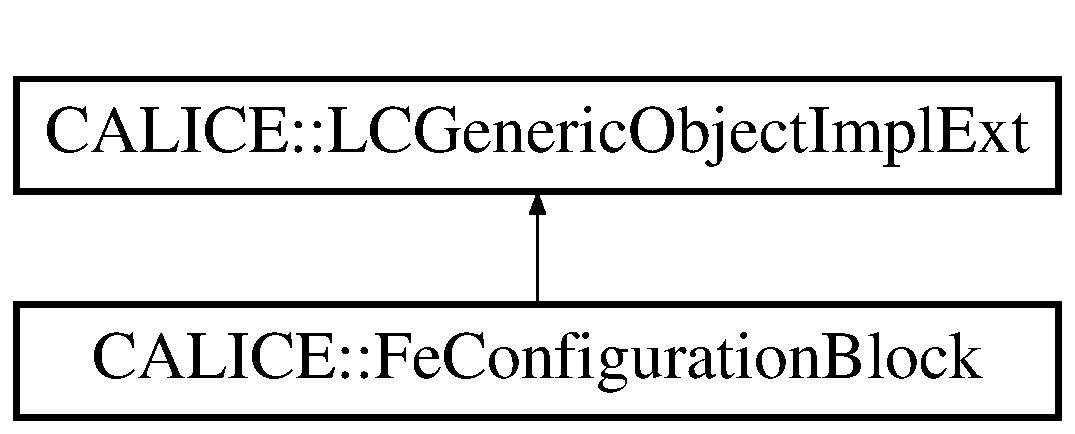
\includegraphics[height=2cm]{classCALICE_1_1FeConfigurationBlock}
\end{center}
\end{figure}
\subsection*{Public Types}
\begin{DoxyCompactItemize}
\item 
enum {\bfseries EFlags} \{ {\bfseries kFlagsCalibEnable} = 1, 
{\bfseries kFlagsHoldInvert} = 2
 \}
\end{DoxyCompactItemize}
\subsection*{Public Member Functions}
\begin{DoxyCompactItemize}
\item 
{\bf FeConfigurationBlock} (int boardID)
\begin{DoxyCompactList}\small\item\em Convenient c'tor. \item\end{DoxyCompactList}\item 
{\bf FeConfigurationBlock} (LCObject $\ast$obj)\label{classCALICE_1_1FeConfigurationBlock_ad308a81b2a293efbfa9b059acfd5cd0a}

\begin{DoxyCompactList}\small\item\em 'Copy constructor' needed to interpret LCCollection read from file/database. \item\end{DoxyCompactList}\item 
{\bf FeConfigurationBlock} \& {\bf setCrateID} (short crateID)\label{classCALICE_1_1FeConfigurationBlock_ae3ce69d5022c5ef8ab80eaa4a5809a49}

\begin{DoxyCompactList}\small\item\em Set the crate ID. \item\end{DoxyCompactList}\item 
short {\bf getCrateID} () const \label{classCALICE_1_1FeConfigurationBlock_a563d030e1ad417a4b34f4f88c8fac9c2}

\begin{DoxyCompactList}\small\item\em Get the crate ID. \item\end{DoxyCompactList}\item 
{\bf FeConfigurationBlock} \& {\bf setSlotID} (short slotID)\label{classCALICE_1_1FeConfigurationBlock_af1379b5cf37a687434a04e5c0e2f3a7d}

\begin{DoxyCompactList}\small\item\em Set the slot ID. \item\end{DoxyCompactList}\item 
short {\bf getSlotID} () const \label{classCALICE_1_1FeConfigurationBlock_a02ff27401b5e03747517a7dc0b6257eb}

\begin{DoxyCompactList}\small\item\em Get the slot ID. \item\end{DoxyCompactList}\item 
{\bf FeConfigurationBlock} \& {\bf setBoardComponentNumber} (short componentNumber)\label{classCALICE_1_1FeConfigurationBlock_a6dfac4b0c8aa3a8928ff990573a1e80e}

\begin{DoxyCompactList}\small\item\em Set the Boardcomponentnumber. \item\end{DoxyCompactList}\item 
short {\bf getBoardComponentNumber} () const \label{classCALICE_1_1FeConfigurationBlock_ab6f0a6007b28356f1c3d91631c8523f9}

\begin{DoxyCompactList}\small\item\em Get the Boardcomponentnumber. \item\end{DoxyCompactList}\item 
void {\bf setRecordLabel} (int label)
\begin{DoxyCompactList}\small\item\em Set the RecordLabel, i.e. \item\end{DoxyCompactList}\item 
short {\bf getRecordLabel} () const \label{classCALICE_1_1FeConfigurationBlock_afe1b8c73434e4d650e9c1e5e069e6d21}

\begin{DoxyCompactList}\small\item\em Get the record label. \item\end{DoxyCompactList}\item 
{\bf FeConfigurationBlock} \& {\bf setBoardID} (int boardID)\label{classCALICE_1_1FeConfigurationBlock_a16507223dc4a936eb23e398b64cdab64}

\begin{DoxyCompactList}\small\item\em Set the boardID composed by crate, slot and component number. \item\end{DoxyCompactList}\item 
int {\bf getBoardID} () const \label{classCALICE_1_1FeConfigurationBlock_a74250fb79bd778eb83550422b605351e}

\begin{DoxyCompactList}\small\item\em Get the boardID. \item\end{DoxyCompactList}\item 
{\bf FeConfigurationBlock} \& {\bf setCalibStart} (int calibStart)
\begin{DoxyCompactList}\small\item\em Set Calibration pulse start value. \item\end{DoxyCompactList}\item 
int {\bf getCalibStart} ()
\begin{DoxyCompactList}\small\item\em Get calibration pulse start value. \item\end{DoxyCompactList}\item 
{\bf FeConfigurationBlock} \& {\bf setCalibWidth} (int calibWidth)
\begin{DoxyCompactList}\small\item\em Set duration of the calibration pulse. \item\end{DoxyCompactList}\item 
int {\bf getCalibWidth} ()
\begin{DoxyCompactList}\small\item\em Get duration of the calibration pulse. \item\end{DoxyCompactList}\item 
{\bf FeConfigurationBlock} \& {\bf setCalibEnable} (bool calib\_\-enable)\label{classCALICE_1_1FeConfigurationBlock_a47922959e144fce64a42999ac95dd70f}

\begin{DoxyCompactList}\small\item\em Se the calib enable value ???? \item\end{DoxyCompactList}\item 
{\bf FeConfigurationBlock} \& {\bf setCalibEnable} ()\label{classCALICE_1_1FeConfigurationBlock_aaa1ae41514efc1703372a25f7177f078}

\begin{DoxyCompactList}\small\item\em Method called by previously defined method ???? \item\end{DoxyCompactList}\item 
{\bf FeConfigurationBlock} \& {\bf clearCalibEnable} ()\label{classCALICE_1_1FeConfigurationBlock_a38cd4c4d715da68c80665b6a776c1f9d}

\begin{DoxyCompactList}\small\item\em clear the calib enable flag \item\end{DoxyCompactList}\item 
bool {\bf isCalibEnable} ()\label{classCALICE_1_1FeConfigurationBlock_a1666f4bfbe633804a10d053b497f9b9a}

\begin{DoxyCompactList}\small\item\em Check the calib enable flag. \item\end{DoxyCompactList}\item 
{\bf FeConfigurationBlock} \& {\bf setHoldStart} (int holdStart)\label{classCALICE_1_1FeConfigurationBlock_a1c0c26a0dc93c4bff4f2421b13b4331d}

\begin{DoxyCompactList}\small\item\em Set the start of holding the signal. \item\end{DoxyCompactList}\item 
int {\bf getHoldStart} ()\label{classCALICE_1_1FeConfigurationBlock_aa128199acd551603835ac602a4d26ab2}

\begin{DoxyCompactList}\small\item\em Get the signel hold start value. \item\end{DoxyCompactList}\item 
{\bf FeConfigurationBlock} \& {\bfseries setHoldWidth} (int holdWidth)\label{classCALICE_1_1FeConfigurationBlock_aa97429cd69298a8a052ac1d8fa074292}

\item 
int {\bf getHoldWidth} ()\label{classCALICE_1_1FeConfigurationBlock_ab9157a0c4cbcf36b26dc41b985e910c5}

\begin{DoxyCompactList}\small\item\em Set the hold width. \item\end{DoxyCompactList}\item 
{\bf FeConfigurationBlock} \& {\bf setHoldInvert} (bool hold\_\-invert)\label{classCALICE_1_1FeConfigurationBlock_a2152b1b5300eca2f4b6effc419f0347c}

\begin{DoxyCompactList}\small\item\em Set whether the holded signal is to be inverted. \item\end{DoxyCompactList}\item 
{\bf FeConfigurationBlock} \& {\bf setHoldInvert} ()\label{classCALICE_1_1FeConfigurationBlock_af8ecb2354dd14ab6c4e508f2daed21a4}

\begin{DoxyCompactList}\small\item\em Method called by previously defined method ???? \item\end{DoxyCompactList}\item 
{\bf FeConfigurationBlock} \& {\bf clearHoldInvert} ()\label{classCALICE_1_1FeConfigurationBlock_abf9d4ad4735645e5d2a98a44fdd40d06}

\begin{DoxyCompactList}\small\item\em Clear the hold invert signel. \item\end{DoxyCompactList}\item 
bool {\bfseries isHoldInvert} ()\label{classCALICE_1_1FeConfigurationBlock_aed101a6b1a554ab8d0b82151f72600f9}

\item 
{\bf FeConfigurationBlock} \& {\bf setVfeResetStart} (int vfeResetStart)\label{classCALICE_1_1FeConfigurationBlock_a34726d417dd6e1d687a10f2b01d83ee8}

\begin{DoxyCompactList}\small\item\em Start of the Vfe Reset. \item\end{DoxyCompactList}\item 
int {\bfseries getVfeResetStart} ()\label{classCALICE_1_1FeConfigurationBlock_aff0543c96dbd09f449fe0bb2d1e669d6}

\item 
{\bf FeConfigurationBlock} \& {\bf setVfeResetEnd} (int vfeResetEnd)\label{classCALICE_1_1FeConfigurationBlock_a339645f629042b5e938a19623ec9a7fa}

\begin{DoxyCompactList}\small\item\em Set the end of the Vfe Reset. \item\end{DoxyCompactList}\item 
int {\bf getVfeResetEnd} ()\label{classCALICE_1_1FeConfigurationBlock_a3a4385a4b617f7600622187bdb6764dd}

\begin{DoxyCompactList}\small\item\em Get the end of the Vfe Reset. \item\end{DoxyCompactList}\item 
{\bf FeConfigurationBlock} \& {\bf setVfeSrinStart} (int vfeSrinStart)\label{classCALICE_1_1FeConfigurationBlock_a58042919f7785d1ca47b4e95e2bdad74}

\begin{DoxyCompactList}\small\item\em I have no idea what the follwing functions really do as long as the data are correct the experts can work with them. \item\end{DoxyCompactList}\item 
int {\bfseries getVfeSrinStart} ()\label{classCALICE_1_1FeConfigurationBlock_aac9d779f7bd4183d3eb143a1f01a514e}

\item 
{\bf FeConfigurationBlock} \& {\bfseries setVfeSrinEnd} (int vfeSrinEnd)\label{classCALICE_1_1FeConfigurationBlock_a6839e0d212773b7cca4e2613fb625d53}

\item 
int {\bfseries getVfeSrinEnd} ()\label{classCALICE_1_1FeConfigurationBlock_a824b9083e874f07e9e33f1696ab1761e}

\item 
{\bf FeConfigurationBlock} \& {\bfseries setVfeMplexClockStart} (int vfeMplexClockStart)\label{classCALICE_1_1FeConfigurationBlock_aec0636a1bf439fb53e8bcdfc3e0ae96e}

\item 
int {\bfseries getVfeMplexClockStart} ()\label{classCALICE_1_1FeConfigurationBlock_a466b3a7b3f357e02f7d784aa05ddcc2e}

\item 
{\bf FeConfigurationBlock} \& {\bfseries setVfeMplexClockMark} (int vfeMplexClockMark)\label{classCALICE_1_1FeConfigurationBlock_a7810ee9b17633bcdeb152fa329b4f153}

\item 
int {\bfseries getVfeMplexClockMark} ()\label{classCALICE_1_1FeConfigurationBlock_a2ab66e21d8a9c82a16c9da2a1629cc7d}

\item 
{\bf FeConfigurationBlock} \& {\bfseries setVfeMplexClockSpace} (int vfeMplexClockSpace)\label{classCALICE_1_1FeConfigurationBlock_a56f9f13c060a99d76e4933a5d2048129}

\item 
int {\bfseries getVfeMplexClockSpace} ()\label{classCALICE_1_1FeConfigurationBlock_a3672f0d174adb315819788ef57c2d31a}

\item 
{\bf FeConfigurationBlock} \& {\bfseries setVfeMplexClockPulses} (int vfeMplexClockPulses)\label{classCALICE_1_1FeConfigurationBlock_a88816754e77a134944edda1fc30b730b}

\item 
int {\bfseries getVfeMplexClockPulses} ()\label{classCALICE_1_1FeConfigurationBlock_aab9112f13270b30c1de654762cd47e42}

\item 
{\bf FeConfigurationBlock} \& {\bf setAdcStart} (int adcStart)\label{classCALICE_1_1FeConfigurationBlock_aa81d30fbb45e727db2f6b15e5e19eaa1}

\begin{DoxyCompactList}\small\item\em Start of the ADC Reading. \item\end{DoxyCompactList}\item 
int {\bfseries getAdcStart} ()\label{classCALICE_1_1FeConfigurationBlock_ab0fa93856bc277f5339ebda4bc9029e8}

\item 
{\bf FeConfigurationBlock} \& {\bf setAdcEnd} (int adcEnd)\label{classCALICE_1_1FeConfigurationBlock_ac84c3e5ce3cdba6b38729ccb6a2994ab}

\begin{DoxyCompactList}\small\item\em End of the ADC Reading, kind of gate width. \item\end{DoxyCompactList}\item 
int {\bfseries getAdcEnd} ()\label{classCALICE_1_1FeConfigurationBlock_a3945433f65d53e796883780d493668a4}

\item 
{\bf FeConfigurationBlock} \& {\bf setAdcControlBits} (int adcControl)\label{classCALICE_1_1FeConfigurationBlock_a855366a700b94188991980a7dc6f874a}

\begin{DoxyCompactList}\small\item\em To whom it may concern ;-\/). \item\end{DoxyCompactList}\item 
int {\bfseries getAdcControlBits} ()\label{classCALICE_1_1FeConfigurationBlock_a7688093dca4620004f2f258e5aceccd9}

\item 
{\bf FeConfigurationBlock} \& {\bf setAdcDelay} (int adcDelay)\label{classCALICE_1_1FeConfigurationBlock_aa292afb028f56f005f00fb612441c96f}

\begin{DoxyCompactList}\small\item\em Delay of the ADC readout. \item\end{DoxyCompactList}\item 
int {\bfseries getAdcDelay} ()\label{classCALICE_1_1FeConfigurationBlock_a861748eff70647d9b61bb1b873a3b72f}

\item 
{\bf FeConfigurationBlock} \& {\bf setDacData} (int top\_\-value, int bottom\_\-value)\label{classCALICE_1_1FeConfigurationBlock_a93df30d4ef75296c3f4b1d0fc530fea2}

\begin{DoxyCompactList}\small\item\em Dac Data setting. \item\end{DoxyCompactList}\item 
int {\bf getDacDataTop} () const \label{classCALICE_1_1FeConfigurationBlock_a0edacda05ba67fe730a5048c762b2a36}

\begin{DoxyCompactList}\small\item\em Daq data on top side of the ADC sample. \item\end{DoxyCompactList}\item 
int {\bf getDacDataBottom} () const \label{classCALICE_1_1FeConfigurationBlock_ad17bbeac4b724a2bae469433c39fabcf}

\begin{DoxyCompactList}\small\item\em Daq data onbottom side of the ADC sample. \item\end{DoxyCompactList}\item 
{\bf FeConfigurationBlock} \& {\bf setFrameSyncDelay} (int frameSyncDelay)\label{classCALICE_1_1FeConfigurationBlock_a91dffce82ee010e9fc2b28e33cb7f659}

\begin{DoxyCompactList}\small\item\em Again not many ideas what this means. \item\end{DoxyCompactList}\item 
int {\bfseries getFrameSyncDelay} ()\label{classCALICE_1_1FeConfigurationBlock_a3f7147f16e7499193371e6309402e011}

\item 
{\bf FeConfigurationBlock} \& {\bfseries setQdrDataDelay} (int qdrDataDelay)\label{classCALICE_1_1FeConfigurationBlock_a6372913f160fb46ba06d9c89da7797c3}

\item 
int {\bfseries getQdrDataDelay} ()\label{classCALICE_1_1FeConfigurationBlock_aa91a26f9caefe64fddd6f9f56f056539}

\item 
{\bf FeConfigurationBlock} \& {\bf setVfeInfo} (int vfeInfo)\label{classCALICE_1_1FeConfigurationBlock_a30ceed6080bb3325a0896fff15559c3f}

\begin{DoxyCompactList}\small\item\em Set Vfe Info for Boards not identified as belonging to the SiW Ecal (only the word itself for the time being. \item\end{DoxyCompactList}\item 
{\bf FeConfigurationBlock} \& {\bf setEmcVfeInfo} (int vfeInfo, int iBot, int iTop, int iBotLowGainBit, int iTopLowGainBit)\label{classCALICE_1_1FeConfigurationBlock_a4c29580324b1b2f9c4aa82df62d5684e}

\begin{DoxyCompactList}\small\item\em Set Vfe Info for the Emc Information. \item\end{DoxyCompactList}\item 
int {\bf getVfeInfo} ()\label{classCALICE_1_1FeConfigurationBlock_ab8d419cc19457884b930ad5e1955f7e7}

\begin{DoxyCompactList}\small\item\em Get complete the Vfe Info. \item\end{DoxyCompactList}\item 
int {\bf emcVfeBottomEnable} (int chip)\label{classCALICE_1_1FeConfigurationBlock_a0c2e92d3989a3d8d0cd8891204d73065}

\begin{DoxyCompactList}\small\item\em Get some detailed emc (!!) vfe info (basically taken from Pauls online software. \item\end{DoxyCompactList}\item 
int {\bfseries emcVfeTopEnable} (int chip)\label{classCALICE_1_1FeConfigurationBlock_a6e93464d42248f7a0107847cf2292c7d}

\item 
bool {\bfseries emcVfeLowGainBottom} ()\label{classCALICE_1_1FeConfigurationBlock_a7ff08d5a8676e1c46559a29182a209ce}

\item 
bool {\bfseries emcVfeLowGainTop} ()\label{classCALICE_1_1FeConfigurationBlock_a9daa373171241b64c93684e3acb2b916}

\item 
void {\bf print} (std::ostream \&os, int)\label{classCALICE_1_1FeConfigurationBlock_abbc1473158e077c3bdba09c9cbbcd5b5}

\begin{DoxyCompactList}\small\item\em Convenient print method. \item\end{DoxyCompactList}\item 
const std::string {\bf getTypeName} () const \label{classCALICE_1_1FeConfigurationBlock_a2ffba337323323ddc6f365ebb8f60d1b}

\begin{DoxyCompactList}\small\item\em Return the type of the class. \item\end{DoxyCompactList}\item 
const std::string {\bf getDataDescription} () const \label{classCALICE_1_1FeConfigurationBlock_a7fd977089ba3e5bde538d861e44a5f2d}

\begin{DoxyCompactList}\small\item\em Return a brief description of the data members. \item\end{DoxyCompactList}\end{DoxyCompactItemize}
\subsection*{Static Public Member Functions}
\begin{DoxyCompactItemize}
\item 
static unsigned int {\bfseries makeBoardID} (const short crateID, const short slotID, const short boardComponentNumber)\label{classCALICE_1_1FeConfigurationBlock_a91dd19e52959ce8e1bb7abd6048f92b7}

\end{DoxyCompactItemize}


\subsection{Detailed Description}
Stores the configuration data of the front-\/end of one CERC board. Based on \doxyref{AdcBlock}{p.}{classCALICE_1_1AdcBlock}. This is just a copy of the Calice DAQ class CrcFeConfigurationData. Since I don't have a profound understanding of the meaning of its members the documentation is mostly missing or at least very poor.

\begin{DoxyAuthor}{Author}
G�tz Gaycken LLR (Ecole Polytechnique) 
\end{DoxyAuthor}
\begin{DoxyDate}{Date}
Apr 2005 
\end{DoxyDate}


Definition at line 58 of file FeConfigurationBlock.hh.

\subsection{Constructor \& Destructor Documentation}
\index{CALICE::FeConfigurationBlock@{CALICE::FeConfigurationBlock}!FeConfigurationBlock@{FeConfigurationBlock}}
\index{FeConfigurationBlock@{FeConfigurationBlock}!CALICE::FeConfigurationBlock@{CALICE::FeConfigurationBlock}}
\subsubsection[{FeConfigurationBlock}]{\setlength{\rightskip}{0pt plus 5cm}CALICE::FeConfigurationBlock::FeConfigurationBlock (int {\em boardID})\hspace{0.3cm}{\ttfamily  [inline]}}\label{classCALICE_1_1FeConfigurationBlock_a1485b6c6c005ca86e5c70aae13a5ec4d}


Convenient c'tor. 
\begin{DoxyParams}{Parameters}
\item[{\em boardID}]CERC board ID (VME crate channel)) \end{DoxyParams}


Definition at line 76 of file FeConfigurationBlock.hh.

References CALICE::LCGenericObjectImplExt::obj().

\subsection{Member Function Documentation}
\index{CALICE::FeConfigurationBlock@{CALICE::FeConfigurationBlock}!getCalibStart@{getCalibStart}}
\index{getCalibStart@{getCalibStart}!CALICE::FeConfigurationBlock@{CALICE::FeConfigurationBlock}}
\subsubsection[{getCalibStart}]{\setlength{\rightskip}{0pt plus 5cm}int CALICE::FeConfigurationBlock::getCalibStart ()\hspace{0.3cm}{\ttfamily  [inline]}}\label{classCALICE_1_1FeConfigurationBlock_a46de3022895df41ce50ed5be8dc4f753}


Get calibration pulse start value. \begin{DoxyReturn}{Returns}
pulse start in units of 6.25 ns. 
\end{DoxyReturn}


Definition at line 172 of file FeConfigurationBlock.hh.\index{CALICE::FeConfigurationBlock@{CALICE::FeConfigurationBlock}!getCalibWidth@{getCalibWidth}}
\index{getCalibWidth@{getCalibWidth}!CALICE::FeConfigurationBlock@{CALICE::FeConfigurationBlock}}
\subsubsection[{getCalibWidth}]{\setlength{\rightskip}{0pt plus 5cm}int CALICE::FeConfigurationBlock::getCalibWidth ()\hspace{0.3cm}{\ttfamily  [inline]}}\label{classCALICE_1_1FeConfigurationBlock_a5eaeeefd9b9d9fe7f4922cfd3589de4c}


Get duration of the calibration pulse. \begin{DoxyReturn}{Returns}
pulse duration in units of 6.25 ns. 
\end{DoxyReturn}


Definition at line 182 of file FeConfigurationBlock.hh.\index{CALICE::FeConfigurationBlock@{CALICE::FeConfigurationBlock}!setCalibStart@{setCalibStart}}
\index{setCalibStart@{setCalibStart}!CALICE::FeConfigurationBlock@{CALICE::FeConfigurationBlock}}
\subsubsection[{setCalibStart}]{\setlength{\rightskip}{0pt plus 5cm}{\bf FeConfigurationBlock}\& CALICE::FeConfigurationBlock::setCalibStart (int {\em calibStart})\hspace{0.3cm}{\ttfamily  [inline]}}\label{classCALICE_1_1FeConfigurationBlock_a41757e805ef1627ab79c1106e0448614}


Set Calibration pulse start value. 
\begin{DoxyParams}{Parameters}
\item[{\em calibStart}]pulse start in units of 6.25 ns. \end{DoxyParams}


Definition at line 167 of file FeConfigurationBlock.hh.

References CALICE::LCGenericObjectImplExt::obj().\index{CALICE::FeConfigurationBlock@{CALICE::FeConfigurationBlock}!setCalibWidth@{setCalibWidth}}
\index{setCalibWidth@{setCalibWidth}!CALICE::FeConfigurationBlock@{CALICE::FeConfigurationBlock}}
\subsubsection[{setCalibWidth}]{\setlength{\rightskip}{0pt plus 5cm}{\bf FeConfigurationBlock}\& CALICE::FeConfigurationBlock::setCalibWidth (int {\em calibWidth})\hspace{0.3cm}{\ttfamily  [inline]}}\label{classCALICE_1_1FeConfigurationBlock_ac01aedde84c305677f215eec469ea277}


Set duration of the calibration pulse. 
\begin{DoxyParams}{Parameters}
\item[{\em calibWidth}]pulse duration in units of 6.25 ns. \end{DoxyParams}


Definition at line 177 of file FeConfigurationBlock.hh.

References CALICE::LCGenericObjectImplExt::obj().\index{CALICE::FeConfigurationBlock@{CALICE::FeConfigurationBlock}!setRecordLabel@{setRecordLabel}}
\index{setRecordLabel@{setRecordLabel}!CALICE::FeConfigurationBlock@{CALICE::FeConfigurationBlock}}
\subsubsection[{setRecordLabel}]{\setlength{\rightskip}{0pt plus 5cm}void CALICE::FeConfigurationBlock::setRecordLabel (int {\em label})\hspace{0.3cm}{\ttfamily  [inline]}}\label{classCALICE_1_1FeConfigurationBlock_a3da15375ce338c89149a9f963a9785d4}


Set the RecordLabel, i.e. whether this dataset was written to or read from a CRC board 

Definition at line 147 of file FeConfigurationBlock.hh.

References CALICE::LCGenericObjectImplExt::obj().

The documentation for this class was generated from the following file:\begin{DoxyCompactItemize}
\item 
FeConfigurationBlock.hh\end{DoxyCompactItemize}

\section{CALICE::FeEvent Class Reference}
\label{classCALICE_1_1FeEvent}\index{CALICE::FeEvent@{CALICE::FeEvent}}


Stores the trigger history (i.e.  


{\ttfamily \#include $<$FeEvent.hh$>$}Inheritance diagram for CALICE::FeEvent::\begin{figure}[H]
\begin{center}
\leavevmode
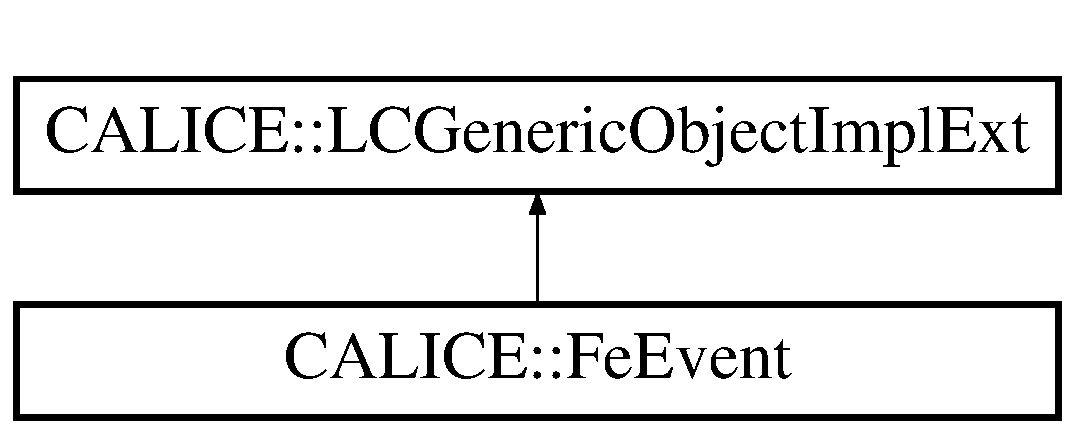
\includegraphics[height=2cm]{classCALICE_1_1FeEvent}
\end{center}
\end{figure}
\subsection*{Public Member Functions}
\begin{DoxyCompactItemize}
\item 
{\bf FeEvent} ()\label{classCALICE_1_1FeEvent_a647e478499ef41c568ebce39db6f31fd}

\begin{DoxyCompactList}\small\item\em Simple Constructor. \item\end{DoxyCompactList}\item 
{\bf FeEvent} (unsigned int board\_\-id)
\begin{DoxyCompactList}\small\item\em UsefulConstructor. \item\end{DoxyCompactList}\item 
{\bf FeEvent} (LCObject $\ast$obj)\label{classCALICE_1_1FeEvent_a7930cd30edc113eb203985a695163c1e}

\begin{DoxyCompactList}\small\item\em 'Copy constructor' needed to interpret LCCollection read from file/database. \item\end{DoxyCompactList}\item 
{\bf FeEvent} \& {\bf setBoardID} (int boardID)
\begin{DoxyCompactList}\small\item\em Set the packed board id. \item\end{DoxyCompactList}\item 
int {\bf getBoardID} () const \label{classCALICE_1_1FeEvent_a8f65bf0bc42c48f9ba41cf2952369052}

\begin{DoxyCompactList}\small\item\em Get the board id. \item\end{DoxyCompactList}\item 
{\bf FeEvent} \& {\bf setRecordLabel} (int label)\label{classCALICE_1_1FeEvent_a75321d2164e0aa9a095f52a0d804e98b}

\begin{DoxyCompactList}\small\item\em Set the Record Label. \item\end{DoxyCompactList}\item 
short {\bf getRecordLabel} () const \label{classCALICE_1_1FeEvent_a36c159cc3f3f014b9dc07978c9016073}

\begin{DoxyCompactList}\small\item\em Return the Record Label. \item\end{DoxyCompactList}\item 
{\bf FeEvent} \& {\bf setTriggerCounter} (int trigger\_\-counter)\label{classCALICE_1_1FeEvent_ad53ef089cf0fd5d1677e3dec63d2f205}

\begin{DoxyCompactList}\small\item\em Set the trigger counter. \item\end{DoxyCompactList}\item 
int {\bf getTriggerCounter} () const \label{classCALICE_1_1FeEvent_a41cc7a30f725675aba016cdbbfbd4953}

\begin{DoxyCompactList}\small\item\em Get the Trigger Counter. \item\end{DoxyCompactList}\item 
{\bf FeEvent} \& {\bf setSpyRegister} (int spyregister)
\begin{DoxyCompactList}\small\item\em Set the Spy Register Value (Whatever this is . \item\end{DoxyCompactList}\item 
int {\bf getSpyRegister} () const \label{classCALICE_1_1FeEvent_a1f3e1d775791b4f28a816def9df16ac2}

\begin{DoxyCompactList}\small\item\em Get the Spy Register Value. \item\end{DoxyCompactList}\item 
void {\bf print} (std::ostream \&os) const \label{classCALICE_1_1FeEvent_a2dd6aa0d8cbd18fe429058cd85197791}

\begin{DoxyCompactList}\small\item\em Convenient print method. \item\end{DoxyCompactList}\item 
const std::string {\bfseries getTypeName} () const \label{classCALICE_1_1FeEvent_a850d7019cf4bcfea521154fe358ba6bc}

\item 
const std::string {\bf getDataDescription} () const \label{classCALICE_1_1FeEvent_ab41ae53dc108e8699b26453a46a7884c}

\begin{DoxyCompactList}\small\item\em Return a brief description of the data members. \item\end{DoxyCompactList}\end{DoxyCompactItemize}


\subsection{Detailed Description}
Stores the trigger history (i.e. fifo content).when it appears in the front end as realized for runs starting in May 2006 (Ask Paul for firmware version) in older versions of the DAQ these data came along wiith the BeTrgEventData which still contains information related to the data handled by the present interface class.

To acces the configuration: 
\begin{DoxyPre}
   void processEvent(LCEvent *event)  \{
       try \{
        // string \_colName = "BeTrgEventData"
        LCCollection *col=event->getCollection(\_colName);
        for (unsigned int element\_i=0; element\_i<col->getNumberOfElements(); element\_i++) \{
           \doxyref{FeEvent}{p.}{classCALICE_1_1FeEvent} event(col->getElementAt(element\_i));\end{DoxyPre}



\begin{DoxyPre}        \}
   \}
 \end{DoxyPre}


\begin{DoxyAuthor}{Author}
R. P�schl (LAL Orsay) 
\end{DoxyAuthor}
\begin{DoxyDate}{Date}
Jul 2006 
\end{DoxyDate}


Definition at line 53 of file FeEvent.hh.

\subsection{Constructor \& Destructor Documentation}
\index{CALICE::FeEvent@{CALICE::FeEvent}!FeEvent@{FeEvent}}
\index{FeEvent@{FeEvent}!CALICE::FeEvent@{CALICE::FeEvent}}
\subsubsection[{FeEvent}]{\setlength{\rightskip}{0pt plus 5cm}CALICE::FeEvent::FeEvent (unsigned int {\em board\_\-id})\hspace{0.3cm}{\ttfamily  [inline]}}\label{classCALICE_1_1FeEvent_a01ee223b5c9ef6ff15712edf275018c8}


UsefulConstructor. 
\begin{DoxyParams}{Parameters}
\item[{\em board\_\-id}]the packed board id (\doxyref{CALICE::BoardID}{p.}{classCALICE_1_1BoardID}). \end{DoxyParams}


Definition at line 72 of file FeEvent.hh.

References setBoardID(), setRecordLabel(), setSpyRegister(), and setTriggerCounter().

\subsection{Member Function Documentation}
\index{CALICE::FeEvent@{CALICE::FeEvent}!setBoardID@{setBoardID}}
\index{setBoardID@{setBoardID}!CALICE::FeEvent@{CALICE::FeEvent}}
\subsubsection[{setBoardID}]{\setlength{\rightskip}{0pt plus 5cm}{\bf FeEvent}\& CALICE::FeEvent::setBoardID (int {\em boardID})\hspace{0.3cm}{\ttfamily  [inline]}}\label{classCALICE_1_1FeEvent_a58128a913587df8b1c25ef444d36b6df}


Set the packed board id. \begin{DoxySeeAlso}{See also}
\doxyref{BoardID}{p.}{classCALICE_1_1BoardID} 
\end{DoxySeeAlso}


Definition at line 91 of file FeEvent.hh.

References CALICE::LCGenericObjectImplExt::obj().

Referenced by FeEvent().\index{CALICE::FeEvent@{CALICE::FeEvent}!setSpyRegister@{setSpyRegister}}
\index{setSpyRegister@{setSpyRegister}!CALICE::FeEvent@{CALICE::FeEvent}}
\subsubsection[{setSpyRegister}]{\setlength{\rightskip}{0pt plus 5cm}{\bf FeEvent}\& CALICE::FeEvent::setSpyRegister (int {\em spyregister})\hspace{0.3cm}{\ttfamily  [inline]}}\label{classCALICE_1_1FeEvent_aa06c38ae89d0db47897f0781e2103115}


Set the Spy Register Value (Whatever this is . ... 

Definition at line 118 of file FeEvent.hh.

References CALICE::LCGenericObjectImplExt::obj().

Referenced by FeEvent().

The documentation for this class was generated from the following files:\begin{DoxyCompactItemize}
\item 
FeEvent.hh\item 
FeEvent.cc\end{DoxyCompactItemize}

\section{CALICE::FeInfo Class Reference}
\label{classCALICE_1_1FeInfo}\index{CALICE::FeInfo@{CALICE::FeInfo}}


Stores the configuration data of the front-\/end of one CERC board.  


{\ttfamily \#include $<$FeInfo.hh$>$}\subsection*{Public Member Functions}
\begin{DoxyCompactItemize}
\item 
{\bf FeInfo} (int boardID)
\begin{DoxyCompactList}\small\item\em Convenient c'tor. \item\end{DoxyCompactList}\item 
int {\bf getBoardID} () const \label{classCALICE_1_1FeInfo_a927351eaab1c2a7281aafbdb19c7cd7a}

\begin{DoxyCompactList}\small\item\em Get the Crc Board ID. \item\end{DoxyCompactList}\item 
{\bf FeInfo} (LCObject $\ast$obj)\label{classCALICE_1_1FeInfo_a46b9df043d100b05f1768e8ea529bce6}

\begin{DoxyCompactList}\small\item\em 'Copy constructor' needed to interpret LCCollection read from file/database. \item\end{DoxyCompactList}\item 
{\bf FeInfo} \& {\bf setLabel} (int label)
\begin{DoxyCompactList}\small\item\em Set the fe link label(?). \item\end{DoxyCompactList}\item 
int {\bf getLabel} () const 
\begin{DoxyCompactList}\small\item\em Get the Fe link label(?). \item\end{DoxyCompactList}\item 
{\bf FeInfo} \& {\bf setFeID} (int fe\_\-id)
\begin{DoxyCompactList}\small\item\em Set the front-\/end id. \item\end{DoxyCompactList}\item 
int {\bf getFeID} () const 
\begin{DoxyCompactList}\small\item\em Get the front-\/end id. \item\end{DoxyCompactList}\item 
{\bf FeInfo} \& {\bf setFrameSyncOut} (int sync\_\-words\_\-01, int sync\_\-words\_\-23, int sync\_\-word\_\-4)
\begin{DoxyCompactList}\small\item\em Set the four frame sync out half words. \item\end{DoxyCompactList}\item 
int {\bf getFrameSyncOut} (int word\_\-i) const 
\begin{DoxyCompactList}\small\item\em Get the frame sync out half words. \item\end{DoxyCompactList}\item 
{\bf FeInfo} \& {\bf setFeLength} (int fe\_\-length)
\begin{DoxyCompactList}\small\item\em Set the fe length field (?). \item\end{DoxyCompactList}\item 
int {\bf getFeLength} () const 
\begin{DoxyCompactList}\small\item\em Get the fe length field (?). \item\end{DoxyCompactList}\item 
{\bf FeInfo} \& {\bf setBeStatus} (int be\_\-status)
\begin{DoxyCompactList}\small\item\em Set the back-\/end status word. \item\end{DoxyCompactList}\item 
int {\bf getBeStatus} () const 
\begin{DoxyCompactList}\small\item\em Get the back-\/end status word. \item\end{DoxyCompactList}\item 
{\bf FeInfo} \& {\bf setTriggerCounter} (int trigger\_\-counter)
\begin{DoxyCompactList}\small\item\em Set the trigger counter. \item\end{DoxyCompactList}\item 
int {\bf getTriggerCounter} () const 
\begin{DoxyCompactList}\small\item\em Get the trigger counter. \item\end{DoxyCompactList}\item 
{\bf FeInfo} \& {\bf setFifo} (int fifo)
\begin{DoxyCompactList}\small\item\em Set the fifo status, and the front-\/end id. \item\end{DoxyCompactList}\item 
int {\bf getFifoFeID} () const 
\begin{DoxyCompactList}\small\item\em Get the front-\/end id from the fifo status word. \item\end{DoxyCompactList}\item 
int {\bf getFifoStatus} () const \label{classCALICE_1_1FeInfo_a753e0ff74eafd5df42eaa0dac24b7a2b}

\begin{DoxyCompactList}\small\item\em Get the fifo status (without front-\/end ID. \item\end{DoxyCompactList}\item 
int {\bf getNumberOfFifoWords} () const \label{classCALICE_1_1FeInfo_a64f44c00899fae956886a44a8c188bdb}

\begin{DoxyCompactList}\small\item\em Get number of words in the fifo. \item\end{DoxyCompactList}\item 
bool {\bf isFifoFull} () const 
\begin{DoxyCompactList}\small\item\em Check whether the fifo is full. \item\end{DoxyCompactList}\item 
bool {\bf isFifoEmpty} () const 
\begin{DoxyCompactList}\small\item\em Check whether the fifo is empty. \item\end{DoxyCompactList}\item 
void {\bf print} (std::ostream \&os) const \label{classCALICE_1_1FeInfo_acc7bde5bd178baec9026df6ccd7f6395}

\begin{DoxyCompactList}\small\item\em Convenient print method. \item\end{DoxyCompactList}\item 
const std::string {\bf getTypeName} () const \label{classCALICE_1_1FeInfo_a3295758439b25dc02172c78b9808e1ff}

\begin{DoxyCompactList}\small\item\em Return the type of the class. \item\end{DoxyCompactList}\item 
const std::string {\bf getDataDescription} () const \label{classCALICE_1_1FeInfo_a53034de0b2da5f70227a548febe27a3c}

\begin{DoxyCompactList}\small\item\em Return a brief description of the data members. \item\end{DoxyCompactList}\end{DoxyCompactItemize}


\subsection{Detailed Description}
Stores the configuration data of the front-\/end of one CERC board. Based on \doxyref{AdcBlock}{p.}{classCALICE_1_1AdcBlock}. This is just a copy of the Calice DAQ class CrcFeConfigurationData. Since I don't have a profound understanding of the meaning of its members the documentation is mostly missing or at least very poor.

\begin{DoxyAuthor}{Author}
G�tz Gaycken LLR (Ecole Polytechnique) 
\end{DoxyAuthor}
\begin{DoxyDate}{Date}
Apr 2005 
\end{DoxyDate}


Definition at line 42 of file FeInfo.hh.

\subsection{Constructor \& Destructor Documentation}
\index{CALICE::FeInfo@{CALICE::FeInfo}!FeInfo@{FeInfo}}
\index{FeInfo@{FeInfo}!CALICE::FeInfo@{CALICE::FeInfo}}
\subsubsection[{FeInfo}]{\setlength{\rightskip}{0pt plus 5cm}CALICE::FeInfo::FeInfo (int {\em boardID})\hspace{0.3cm}{\ttfamily  [inline]}}\label{classCALICE_1_1FeInfo_a4db195f856cb913c1dc1b7abe558dd07}


Convenient c'tor. 
\begin{DoxyParams}{Parameters}
\item[{\em boardID}]Crc board ID (VME crate, slot, fe)) \end{DoxyParams}


Definition at line 50 of file FeInfo.hh.

\subsection{Member Function Documentation}
\index{CALICE::FeInfo@{CALICE::FeInfo}!getBeStatus@{getBeStatus}}
\index{getBeStatus@{getBeStatus}!CALICE::FeInfo@{CALICE::FeInfo}}
\subsubsection[{getBeStatus}]{\setlength{\rightskip}{0pt plus 5cm}int CALICE::FeInfo::getBeStatus () const\hspace{0.3cm}{\ttfamily  [inline]}}\label{classCALICE_1_1FeInfo_a56f6bb4e32c6016da0cedbbc86050c1a}


Get the back-\/end status word. \begin{Desc}
\item[{\bf Todo}]needs better explanation. \end{Desc}


Definition at line 163 of file FeInfo.hh.

Referenced by print().\index{CALICE::FeInfo@{CALICE::FeInfo}!getFeID@{getFeID}}
\index{getFeID@{getFeID}!CALICE::FeInfo@{CALICE::FeInfo}}
\subsubsection[{getFeID}]{\setlength{\rightskip}{0pt plus 5cm}int CALICE::FeInfo::getFeID () const\hspace{0.3cm}{\ttfamily  [inline]}}\label{classCALICE_1_1FeInfo_a9632e47d7dad152f6b354ef9be4ba125}


Get the front-\/end id. This field is redundant since the front-\/end id is also encoded in the board ID. 

Definition at line 81 of file FeInfo.hh.

Referenced by print().\index{CALICE::FeInfo@{CALICE::FeInfo}!getFeLength@{getFeLength}}
\index{getFeLength@{getFeLength}!CALICE::FeInfo@{CALICE::FeInfo}}
\subsubsection[{getFeLength}]{\setlength{\rightskip}{0pt plus 5cm}int CALICE::FeInfo::getFeLength () const\hspace{0.3cm}{\ttfamily  [inline]}}\label{classCALICE_1_1FeInfo_a8670ba7cf2806521398a0ad5b3081889}


Get the fe length field (?). \begin{Desc}
\item[{\bf Todo}]needs better explanation. \end{Desc}


Definition at line 140 of file FeInfo.hh.

Referenced by print().\index{CALICE::FeInfo@{CALICE::FeInfo}!getFifoFeID@{getFifoFeID}}
\index{getFifoFeID@{getFifoFeID}!CALICE::FeInfo@{CALICE::FeInfo}}
\subsubsection[{getFifoFeID}]{\setlength{\rightskip}{0pt plus 5cm}int CALICE::FeInfo::getFifoFeID () const\hspace{0.3cm}{\ttfamily  [inline]}}\label{classCALICE_1_1FeInfo_a11143b4aea8cc4623c53a3327de74d29}


Get the front-\/end id from the fifo status word. If this front-\/end id does not match the result of \doxyref{getFeID}{p.}{classCALICE_1_1FeInfo_a9632e47d7dad152f6b354ef9be4ba125} then all the front-\/end data for this particular event is corrupt. 

Definition at line 186 of file FeInfo.hh.

Referenced by print().\index{CALICE::FeInfo@{CALICE::FeInfo}!getFrameSyncOut@{getFrameSyncOut}}
\index{getFrameSyncOut@{getFrameSyncOut}!CALICE::FeInfo@{CALICE::FeInfo}}
\subsubsection[{getFrameSyncOut}]{\setlength{\rightskip}{0pt plus 5cm}int CALICE::FeInfo::getFrameSyncOut (int {\em word\_\-i}) const\hspace{0.3cm}{\ttfamily  [inline]}}\label{classCALICE_1_1FeInfo_adf4bfb5cd87315ffc2e20b1032431eee}


Get the frame sync out half words. 
\begin{DoxyParams}{Parameters}
\item[{\em word\_\-i}]the index of the word (valid range 0-\/4). \end{DoxyParams}
\begin{DoxyReturn}{Returns}
the specified 16 bit half word. 
\end{DoxyReturn}


Definition at line 106 of file FeInfo.hh.

Referenced by print().\index{CALICE::FeInfo@{CALICE::FeInfo}!getLabel@{getLabel}}
\index{getLabel@{getLabel}!CALICE::FeInfo@{CALICE::FeInfo}}
\subsubsection[{getLabel}]{\setlength{\rightskip}{0pt plus 5cm}int CALICE::FeInfo::getLabel () const\hspace{0.3cm}{\ttfamily  [inline]}}\label{classCALICE_1_1FeInfo_a67dd0f689121876bcae54f69813c29dd}


Get the Fe link label(?). \begin{Desc}
\item[{\bf Todo}]needs better explanation. \end{Desc}


Definition at line 71 of file FeInfo.hh.

Referenced by print().\index{CALICE::FeInfo@{CALICE::FeInfo}!getTriggerCounter@{getTriggerCounter}}
\index{getTriggerCounter@{getTriggerCounter}!CALICE::FeInfo@{CALICE::FeInfo}}
\subsubsection[{getTriggerCounter}]{\setlength{\rightskip}{0pt plus 5cm}int CALICE::FeInfo::getTriggerCounter () const\hspace{0.3cm}{\ttfamily  [inline]}}\label{classCALICE_1_1FeInfo_a2ed250cf245576cd1b4a13a68132f38b}


Get the trigger counter. The trigger counter can be used to identify front-\/end data of the same event. 

Definition at line 175 of file FeInfo.hh.

Referenced by print().\index{CALICE::FeInfo@{CALICE::FeInfo}!isFifoEmpty@{isFifoEmpty}}
\index{isFifoEmpty@{isFifoEmpty}!CALICE::FeInfo@{CALICE::FeInfo}}
\subsubsection[{isFifoEmpty}]{\setlength{\rightskip}{0pt plus 5cm}bool CALICE::FeInfo::isFifoEmpty () const\hspace{0.3cm}{\ttfamily  [inline]}}\label{classCALICE_1_1FeInfo_ab91279ac76ce115a090860ad8c105c5e}


Check whether the fifo is empty. \begin{DoxyReturn}{Returns}
true if the fifo is empty; 
\end{DoxyReturn}


Definition at line 206 of file FeInfo.hh.

Referenced by print().\index{CALICE::FeInfo@{CALICE::FeInfo}!isFifoFull@{isFifoFull}}
\index{isFifoFull@{isFifoFull}!CALICE::FeInfo@{CALICE::FeInfo}}
\subsubsection[{isFifoFull}]{\setlength{\rightskip}{0pt plus 5cm}bool CALICE::FeInfo::isFifoFull () const\hspace{0.3cm}{\ttfamily  [inline]}}\label{classCALICE_1_1FeInfo_abaf3c49388c8673c44e35de0dd2a5d7d}


Check whether the fifo is full. \begin{DoxyReturn}{Returns}
true if the fifo is full; 
\end{DoxyReturn}


Definition at line 201 of file FeInfo.hh.

Referenced by print().\index{CALICE::FeInfo@{CALICE::FeInfo}!setBeStatus@{setBeStatus}}
\index{setBeStatus@{setBeStatus}!CALICE::FeInfo@{CALICE::FeInfo}}
\subsubsection[{setBeStatus}]{\setlength{\rightskip}{0pt plus 5cm}{\bf FeInfo}\& CALICE::FeInfo::setBeStatus (int {\em be\_\-status})\hspace{0.3cm}{\ttfamily  [inline]}}\label{classCALICE_1_1FeInfo_a04552f8e75412662946c7b3c65dad0c5}


Set the back-\/end status word. \begin{Desc}
\item[{\bf Todo}]needs better explanation. \end{Desc}


Definition at line 149 of file FeInfo.hh.\index{CALICE::FeInfo@{CALICE::FeInfo}!setFeID@{setFeID}}
\index{setFeID@{setFeID}!CALICE::FeInfo@{CALICE::FeInfo}}
\subsubsection[{setFeID}]{\setlength{\rightskip}{0pt plus 5cm}{\bf FeInfo}\& CALICE::FeInfo::setFeID (int {\em fe\_\-id})\hspace{0.3cm}{\ttfamily  [inline]}}\label{classCALICE_1_1FeInfo_a723e578651833bb2c038a95920d47da8}


Set the front-\/end id. This field is redundant since the front-\/end id is also encoded in the board ID. 

Definition at line 76 of file FeInfo.hh.\index{CALICE::FeInfo@{CALICE::FeInfo}!setFeLength@{setFeLength}}
\index{setFeLength@{setFeLength}!CALICE::FeInfo@{CALICE::FeInfo}}
\subsubsection[{setFeLength}]{\setlength{\rightskip}{0pt plus 5cm}{\bf FeInfo}\& CALICE::FeInfo::setFeLength (int {\em fe\_\-length})\hspace{0.3cm}{\ttfamily  [inline]}}\label{classCALICE_1_1FeInfo_a884328110730cf0cb15c96aed00d3930}


Set the fe length field (?). \begin{Desc}
\item[{\bf Todo}]needs better explanation. \end{Desc}


Definition at line 130 of file FeInfo.hh.\index{CALICE::FeInfo@{CALICE::FeInfo}!setFifo@{setFifo}}
\index{setFifo@{setFifo}!CALICE::FeInfo@{CALICE::FeInfo}}
\subsubsection[{setFifo}]{\setlength{\rightskip}{0pt plus 5cm}{\bf FeInfo}\& CALICE::FeInfo::setFifo (int {\em fifo})\hspace{0.3cm}{\ttfamily  [inline]}}\label{classCALICE_1_1FeInfo_a8c41e4ec923a8ac88ef4922ad6223fe4}


Set the fifo status, and the front-\/end id. 
\begin{DoxyParams}{Parameters}
\item[{\em fifo}]the packed word which contains the front-\/end id, and the fifo status (overflow/underflow bits, fifo words). \end{DoxyParams}


Definition at line 180 of file FeInfo.hh.\index{CALICE::FeInfo@{CALICE::FeInfo}!setFrameSyncOut@{setFrameSyncOut}}
\index{setFrameSyncOut@{setFrameSyncOut}!CALICE::FeInfo@{CALICE::FeInfo}}
\subsubsection[{setFrameSyncOut}]{\setlength{\rightskip}{0pt plus 5cm}{\bf FeInfo}\& CALICE::FeInfo::setFrameSyncOut (int {\em sync\_\-words\_\-01}, \/  int {\em sync\_\-words\_\-23}, \/  int {\em sync\_\-word\_\-4})\hspace{0.3cm}{\ttfamily  [inline]}}\label{classCALICE_1_1FeInfo_a6362120a57541cab907c7d4a7a53a6a7}


Set the four frame sync out half words. 
\begin{DoxyParams}{Parameters}
\item[{\em sync\_\-words\_\-01}]the first and the second half word packed in one 32bit integer. \item[{\em sync\_\-words\_\-23}]the third and the forth half word packed in one 32bit integer. \item[{\em sync\_\-word\_\-4}]the fifth half word packed in the lower 16 bits of a 32bit integer.\end{DoxyParams}
The first word should be in the lower 16 bit of the first argument, the second word in the upper 16 bits of the first argument and so forth: 


\begin{DoxyPre}
 sync\_words\_01= (word\_0 \& 0xffff) + ((word\_1 \& xffff)<<16);
 \end{DoxyPre}
 

Definition at line 95 of file FeInfo.hh.\index{CALICE::FeInfo@{CALICE::FeInfo}!setLabel@{setLabel}}
\index{setLabel@{setLabel}!CALICE::FeInfo@{CALICE::FeInfo}}
\subsubsection[{setLabel}]{\setlength{\rightskip}{0pt plus 5cm}{\bf FeInfo}\& CALICE::FeInfo::setLabel (int {\em label})\hspace{0.3cm}{\ttfamily  [inline]}}\label{classCALICE_1_1FeInfo_a30d1e319c5b493268ee8f8674a9f0f6c}


Set the fe link label(?). \begin{Desc}
\item[{\bf Todo}]needs better explanation. \end{Desc}


Definition at line 66 of file FeInfo.hh.\index{CALICE::FeInfo@{CALICE::FeInfo}!setTriggerCounter@{setTriggerCounter}}
\index{setTriggerCounter@{setTriggerCounter}!CALICE::FeInfo@{CALICE::FeInfo}}
\subsubsection[{setTriggerCounter}]{\setlength{\rightskip}{0pt plus 5cm}{\bf FeInfo}\& CALICE::FeInfo::setTriggerCounter (int {\em trigger\_\-counter})\hspace{0.3cm}{\ttfamily  [inline]}}\label{classCALICE_1_1FeInfo_ac83132aaa58beefd0c465385cdd35e75}


Set the trigger counter. The trigger counter can be used to identify front-\/end data of the same event. 

Definition at line 170 of file FeInfo.hh.

The documentation for this class was generated from the following files:\begin{DoxyCompactItemize}
\item 
FeInfo.hh\item 
FeInfo.cc\end{DoxyCompactItemize}

\section{FeStatList\_\-t$<$ T\_\-StatObj\_\-t $>$ Class Template Reference}
\label{classFeStatList__t}\index{FeStatList\_\-t@{FeStatList\_\-t}}


Template container which stores specific statistics objects per front-\/end.  


{\ttfamily \#include $<$FeStatList\_\-t.hh$>$}Inheritance diagram for FeStatList\_\-t$<$ T\_\-StatObj\_\-t $>$::\begin{figure}[H]
\begin{center}
\leavevmode
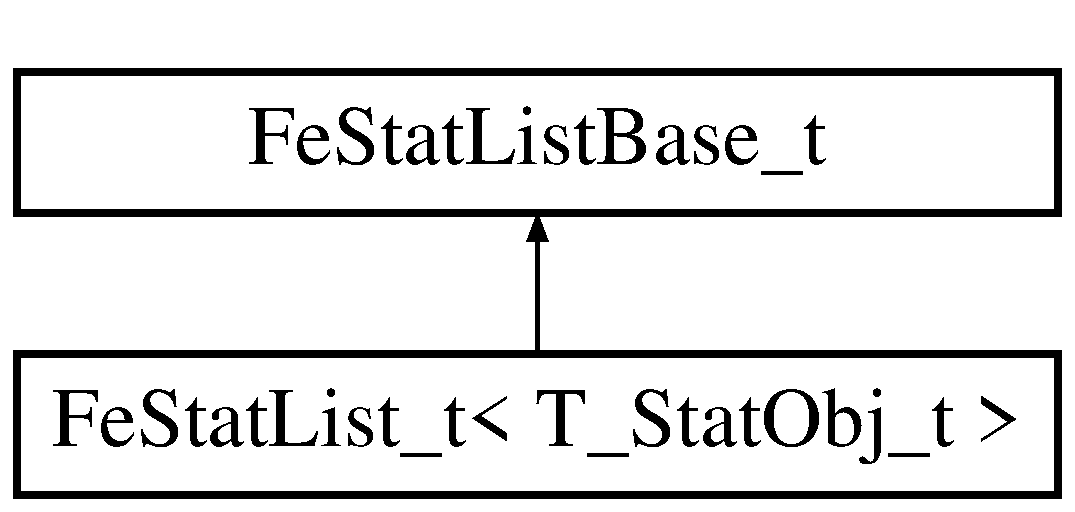
\includegraphics[height=2cm]{classFeStatList__t}
\end{center}
\end{figure}
\subsection*{Public Member Functions}
\begin{DoxyCompactItemize}
\item 
T\_\-StatObj\_\-t \& {\bf getStat} (unsigned int board\_\-id)
\begin{DoxyCompactList}\small\item\em Get a statistics object for the given front-\/end. \item\end{DoxyCompactList}\end{DoxyCompactItemize}


\subsection{Detailed Description}
\subsubsection*{template$<$class T\_\-StatObj\_\-t$>$ class FeStatList\_\-t$<$ T\_\-StatObj\_\-t $>$}

Template container which stores specific statistics objects per front-\/end. The statistics can be printed 

Definition at line 144 of file FeStatList\_\-t.hh.

\subsection{Member Function Documentation}
\index{FeStatList\_\-t@{FeStatList\_\-t}!getStat@{getStat}}
\index{getStat@{getStat}!FeStatList_t@{FeStatList\_\-t}}
\subsubsection[{getStat}]{\setlength{\rightskip}{0pt plus 5cm}template$<$class T\_\-StatObj\_\-t $>$ T\_\-StatObj\_\-t\& {\bf FeStatList\_\-t}$<$ T\_\-StatObj\_\-t $>$::getStat (unsigned int {\em board\_\-id})\hspace{0.3cm}{\ttfamily  [inline]}}\label{classFeStatList__t_a5b29ca60859d52c5e2279f9636ac6b01}


Get a statistics object for the given front-\/end. 
\begin{DoxyParams}{Parameters}
\item[{\em board\_\-id}]the id of the crate,slot and front-\/end. If no statistics object exists for the given front-\/end then a new object is created using the default constructor i.e. the objects T\_\-StatObj\_\-t must implement a default constructor. \end{DoxyParams}


Reimplemented from {\bf FeStatListBase\_\-t} \doxyref{}{p.}{classFeStatListBase__t_af736c1e9e3e131095ac69d5b7448ce6f}.

Definition at line 153 of file FeStatList\_\-t.hh.

The documentation for this class was generated from the following file:\begin{DoxyCompactItemize}
\item 
FeStatList\_\-t.hh\end{DoxyCompactItemize}

\section{FeStatListBase\_\-t Class Reference}
\label{classFeStatListBase__t}\index{FeStatListBase\_\-t@{FeStatListBase\_\-t}}


Container class which can store statistics objects for all existing front-\/ends.  


{\ttfamily \#include $<$FeStatList\_\-t.hh$>$}Inheritance diagram for FeStatListBase\_\-t::\begin{figure}[H]
\begin{center}
\leavevmode
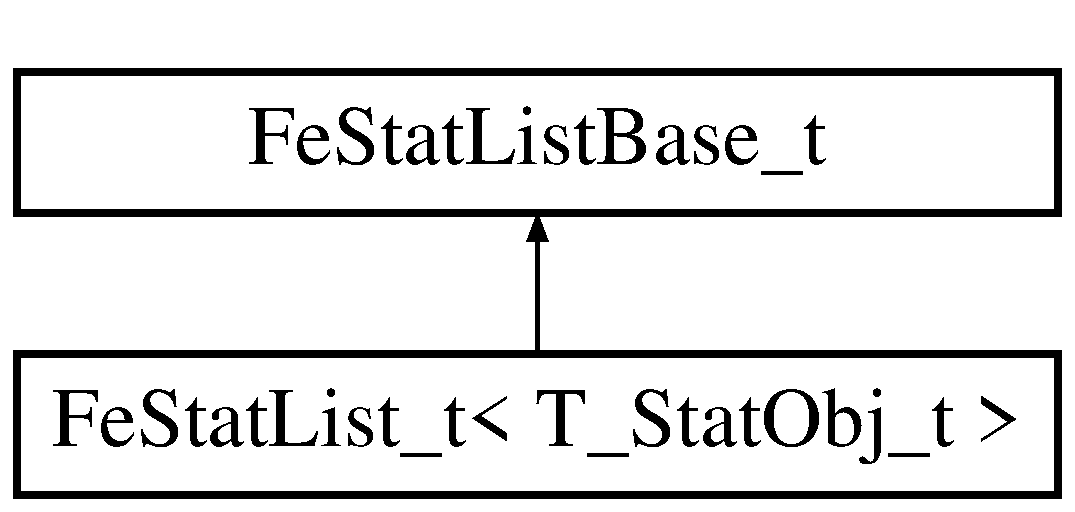
\includegraphics[height=2cm]{classFeStatListBase__t}
\end{center}
\end{figure}
\subsection*{Public Member Functions}
\begin{DoxyCompactItemize}
\item 
void {\bf show} (const char $\ast$label)
\begin{DoxyCompactList}\small\item\em Print statistics about all front-\/ends. \item\end{DoxyCompactList}\end{DoxyCompactItemize}
\subsection*{Protected Types}
\begin{DoxyCompactItemize}
\item 
typedef {\bf StatObj\_\-t} $\ast$ {\bfseries StatObjPtr}\label{classFeStatListBase__t_a375c72380cafb0c98dfc80cbd1d0305f}

\end{DoxyCompactItemize}
\subsection*{Protected Member Functions}
\begin{DoxyCompactItemize}
\item 
{\bf StatObjPtr} \& {\bf getStat} (unsigned int board\_\-id)
\begin{DoxyCompactList}\small\item\em Get the statistics object for the given board id. \item\end{DoxyCompactList}\end{DoxyCompactItemize}
\subsection*{Private Attributes}
\begin{DoxyCompactItemize}
\item 
std::map$<$ unsigned int, std::vector$<$ std::vector$<$ {\bf StatObjPtr} $>$ $>$ $>$ {\bfseries \_\-feInfo}\label{classFeStatListBase__t_aa6de25584603d7826ea405b0d56dd0ff}

\end{DoxyCompactItemize}


\subsection{Detailed Description}
Container class which can store statistics objects for all existing front-\/ends. The statistics collected from all front-\/ends can be printed to an output stream. {\bfseries This class should not be used directly but the template \doxyref{FeStatList\_\-t}{p.}{classFeStatList__t}} which gives You type safety. 

Definition at line 59 of file FeStatList\_\-t.hh.

\subsection{Member Function Documentation}
\index{FeStatListBase\_\-t@{FeStatListBase\_\-t}!getStat@{getStat}}
\index{getStat@{getStat}!FeStatListBase_t@{FeStatListBase\_\-t}}
\subsubsection[{getStat}]{\setlength{\rightskip}{0pt plus 5cm}{\bf StatObjPtr}\& FeStatListBase\_\-t::getStat (unsigned int {\em board\_\-id})\hspace{0.3cm}{\ttfamily  [inline, protected]}}\label{classFeStatListBase__t_af736c1e9e3e131095ac69d5b7448ce6f}


Get the statistics object for the given board id. 
\begin{DoxyParams}{Parameters}
\item[{\em board\_\-id}]id which tells the crate, slot and front-\/end. This method should not be used directly but the template \doxyref{FeStatList\_\-t::getStat}{p.}{classFeStatList__t_a5b29ca60859d52c5e2279f9636ac6b01} \end{DoxyParams}


Reimplemented in {\bf FeStatList\_\-t$<$ T\_\-StatObj\_\-t $>$} \doxyref{}{p.}{classFeStatList__t_a5b29ca60859d52c5e2279f9636ac6b01}.

Definition at line 86 of file FeStatList\_\-t.hh.

References CALICE::BoardID::getBoardComponentNumber(), CALICE::BoardID::getCrateID(), and CALICE::BoardID::getSlotID().\index{FeStatListBase\_\-t@{FeStatListBase\_\-t}!show@{show}}
\index{show@{show}!FeStatListBase_t@{FeStatListBase\_\-t}}
\subsubsection[{show}]{\setlength{\rightskip}{0pt plus 5cm}void FeStatListBase\_\-t::show (const char $\ast$ {\em label})}\label{classFeStatListBase__t_af8d07bf048c14d95c95338c3d1b10f91}


Print statistics about all front-\/ends. 
\begin{DoxyParams}{Parameters}
\item[{\em label}]text to be printed as a header line. The output depends on the statistics objects used. {\bfseries NOTE:} This method will call the method \doxyref{StatObj\_\-t::finish}{p.}{classStatObj__t_a47e9637e59dc8e2cb5889de98160e553} i.e. the objects should not be changed afterwords otherwise the result will rather undefined. \end{DoxyParams}


Definition at line 24 of file FeStatList\_\-t.cc.

The documentation for this class was generated from the following files:\begin{DoxyCompactItemize}
\item 
FeStatList\_\-t.hh\item 
FeStatList\_\-t.cc\end{DoxyCompactItemize}

\section{CALICE::FeTrgData Class Reference}
\label{classCALICE_1_1FeTrgData}\index{CALICE::FeTrgData@{CALICE::FeTrgData}}


Stores the trigger history (i.e.  


{\ttfamily \#include $<$FeTrgData.hh$>$}Inheritance diagram for CALICE::FeTrgData::\begin{figure}[H]
\begin{center}
\leavevmode
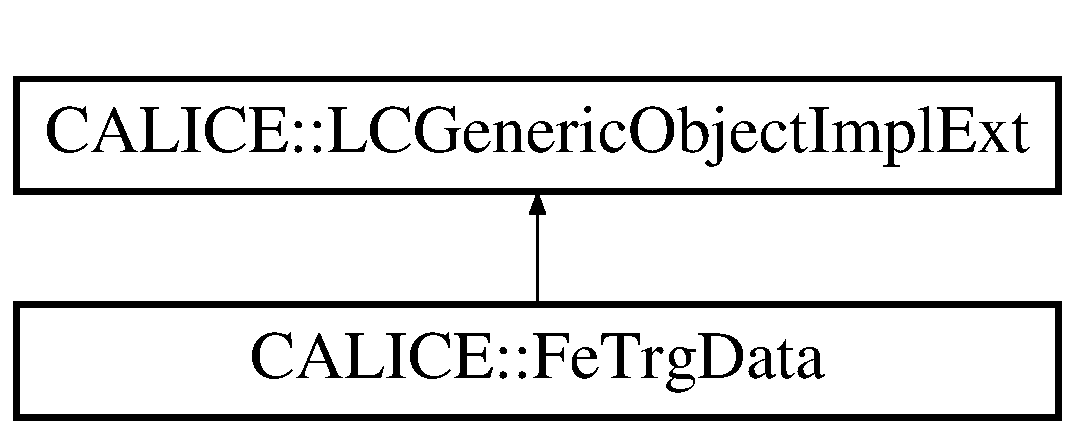
\includegraphics[height=2cm]{classCALICE_1_1FeTrgData}
\end{center}
\end{figure}
\subsection*{Public Member Functions}
\begin{DoxyCompactItemize}
\item 
{\bf FeTrgData} (unsigned int board\_\-id)
\begin{DoxyCompactList}\small\item\em UsefulConstructor. \item\end{DoxyCompactList}\item 
{\bf FeTrgData} (LCObject $\ast$obj)\label{classCALICE_1_1FeTrgData_ae4699322e9026b8a3ee23a30d41eb286}

\begin{DoxyCompactList}\small\item\em 'Copy constructor' needed to interpret LCCollection read from file/database. \item\end{DoxyCompactList}\item 
{\bf FeTrgData} \& {\bf setBoardID} (int boardID)
\begin{DoxyCompactList}\small\item\em set the packed board id. \item\end{DoxyCompactList}\item 
int {\bf getBoardID} () const \label{classCALICE_1_1FeTrgData_ab209441abacd771419e405827eedbf9b}

\begin{DoxyCompactList}\small\item\em Get the board id. \item\end{DoxyCompactList}\item 
{\bf FeTrgData} \& {\bf setRecordLabel} (int label)
\begin{DoxyCompactList}\small\item\em set the record label. \item\end{DoxyCompactList}\item 
int {\bf getRecordLabel} () const \label{classCALICE_1_1FeTrgData_a8af2b4f79f761ed922bda71ca34a2e35}

\begin{DoxyCompactList}\small\item\em get the record label \item\end{DoxyCompactList}\item 
{\bf FeTrgData} \& {\bf setHeaderWord} (int header)\label{classCALICE_1_1FeTrgData_a031101248fdcc6bd674f5f0a20076519}

\begin{DoxyCompactList}\small\item\em The header which comes along with the CrcVlinkTrgData. \item\end{DoxyCompactList}\item 
int {\bf getHeaderWord} () const \label{classCALICE_1_1FeTrgData_aee7c5d27435bb47dcc5a0fa7195f19de}

\begin{DoxyCompactList}\small\item\em Get the header word. \item\end{DoxyCompactList}\item 
{\bf FeTrgData} \& {\bf setTrailerWord} (int trailer)\label{classCALICE_1_1FeTrgData_aba4ddaa52d268934f26a4c7bfa9c7726}

\begin{DoxyCompactList}\small\item\em The trailer which comes along with the CrcVlinkTrgData. \item\end{DoxyCompactList}\item 
int {\bf getTrailerWord} () const \label{classCALICE_1_1FeTrgData_a5ffb1789508a8dde836d3da88ef5b872}

\begin{DoxyCompactList}\small\item\em Get the trailer word. \item\end{DoxyCompactList}\item 
{\bf FeTrgData} \& {\bf setTriggerCounter} (int trigcount)\label{classCALICE_1_1FeTrgData_a1f7fda609b65e41d3d6622139a75b015}

\begin{DoxyCompactList}\small\item\em Set the trigger counter (=trigger number). \item\end{DoxyCompactList}\item 
int {\bf getTriggerCounter} () const \label{classCALICE_1_1FeTrgData_a2084f1b7da4ba0606e8a861ab67be29c}

\begin{DoxyCompactList}\small\item\em Get the trigger number. \item\end{DoxyCompactList}\item 
{\bf FeTrgData} \& {\bf setFifoWord} (unsigned int word\_\-index, unsigned int word)
\begin{DoxyCompactList}\small\item\em Set the fifo word. \item\end{DoxyCompactList}\item 
{\bf FeTrgData} \& {\bf setAllFifoWords} (unsigned int n\_\-words, const unsigned int $\ast$const word\_\-list)
\begin{DoxyCompactList}\small\item\em Set all the fifo words. \item\end{DoxyCompactList}\item 
int {\bf getNFifoWords} () const \label{classCALICE_1_1FeTrgData_a6a008a08e6e3c7b13c9feecb7287dcbe}

\begin{DoxyCompactList}\small\item\em Get the number of words contained in the fifo. \item\end{DoxyCompactList}\item 
int {\bf getFifoWord} (unsigned int word\_\-index) const 
\begin{DoxyCompactList}\small\item\em Get a fifo word. \item\end{DoxyCompactList}\item 
IntVec \& {\bf getFifoWords} (IntVec \&dest) const 
\begin{DoxyCompactList}\small\item\em Get a fifo word. \item\end{DoxyCompactList}\item 
void {\bf print} (std::ostream \&os)\label{classCALICE_1_1FeTrgData_a6bc8fda20344fc0554c651285d3dfa1a}

\begin{DoxyCompactList}\small\item\em Convenient print method. \item\end{DoxyCompactList}\item 
const std::string {\bfseries getTypeName} () const \label{classCALICE_1_1FeTrgData_a4923ab06fbee197d93dad21ca8f30ed2}

\item 
const std::string {\bf getDataDescription} () const \label{classCALICE_1_1FeTrgData_abf24441f6eb134ea939fd4028b6b5cf7}

\begin{DoxyCompactList}\small\item\em Return a brief description of the data members. \item\end{DoxyCompactList}\end{DoxyCompactItemize}


\subsection{Detailed Description}
Stores the trigger history (i.e. fifo content).when it appears in the front end as realized for runs starting in May 2006 (Ask Paul for firmware version) in older versions of the DAQ these data came along wiith the BeTrgEventData which still contains information related to the data handled by the present interface class.

To acces the configuration: 
\begin{DoxyPre}
   void processEvent(LCEvent *event)  \{
       try \{
        // string \_colName = "BeTrgEventData"
        LCCollection *col=event->getCollection(\_colName);
        for (unsigned int element\_i=0; element\_i<col->getNumberOfElements(); element\_i++) \{
           \doxyref{BeTrgEvent}{p.}{classCALICE_1_1BeTrgEvent} event(col->getElementAt(element\_i));\end{DoxyPre}



\begin{DoxyPre}        \}
   \}
 \end{DoxyPre}


\begin{DoxyAuthor}{Author}
R. P�schl (LAL Orsay) 
\end{DoxyAuthor}
\begin{DoxyDate}{Date}
Jul 2006 
\end{DoxyDate}


Definition at line 56 of file FeTrgData.hh.

\subsection{Constructor \& Destructor Documentation}
\index{CALICE::FeTrgData@{CALICE::FeTrgData}!FeTrgData@{FeTrgData}}
\index{FeTrgData@{FeTrgData}!CALICE::FeTrgData@{CALICE::FeTrgData}}
\subsubsection[{FeTrgData}]{\setlength{\rightskip}{0pt plus 5cm}CALICE::FeTrgData::FeTrgData (unsigned int {\em board\_\-id})\hspace{0.3cm}{\ttfamily  [inline]}}\label{classCALICE_1_1FeTrgData_a1839aae65e73c22b7827f32e3f2acc04}


UsefulConstructor. 
\begin{DoxyParams}{Parameters}
\item[{\em board\_\-id}]the packed board id (\doxyref{CALICE::BoardID}{p.}{classCALICE_1_1BoardID}). \end{DoxyParams}


Definition at line 64 of file FeTrgData.hh.

References setBoardID(), setHeaderWord(), setRecordLabel(), setTrailerWord(), and setTriggerCounter().

\subsection{Member Function Documentation}
\index{CALICE::FeTrgData@{CALICE::FeTrgData}!getFifoWord@{getFifoWord}}
\index{getFifoWord@{getFifoWord}!CALICE::FeTrgData@{CALICE::FeTrgData}}
\subsubsection[{getFifoWord}]{\setlength{\rightskip}{0pt plus 5cm}int CALICE::FeTrgData::getFifoWord (unsigned int {\em word\_\-index}) const\hspace{0.3cm}{\ttfamily  [inline]}}\label{classCALICE_1_1FeTrgData_acec138b6d2208c16c2918ce7a94050db}


Get a fifo word. 
\begin{DoxyParams}{Parameters}
\item[{\em word\_\-index}]of the word in the fifo. \end{DoxyParams}


Definition at line 156 of file FeTrgData.hh.

References getNFifoWords().

Referenced by getFifoWords(), and print().\index{CALICE::FeTrgData@{CALICE::FeTrgData}!getFifoWords@{getFifoWords}}
\index{getFifoWords@{getFifoWords}!CALICE::FeTrgData@{CALICE::FeTrgData}}
\subsubsection[{getFifoWords}]{\setlength{\rightskip}{0pt plus 5cm}IntVec\& CALICE::FeTrgData::getFifoWords (IntVec \& {\em dest}) const\hspace{0.3cm}{\ttfamily  [inline]}}\label{classCALICE_1_1FeTrgData_a948057cbcdd6783699a7571654582e83}


Get a fifo word. 
\begin{DoxyParams}{Parameters}
\item[{\em dest}]reference to a vector of integers whiich will be cleared in filled with the contents of the fifo. \end{DoxyParams}
\begin{DoxyReturn}{Returns}
for convenience a reference to the filled vector (i.e. is the one given as argument).
\end{DoxyReturn}
NOTE: Unless a vector is needed to pass the data to some function, it is adviced to get the individual values with \doxyref{getFifoWord()}{p.}{classCALICE_1_1FeTrgData_acec138b6d2208c16c2918ce7a94050db} since this avoids copying (On the other hand, each access has the penalty of a virtual function call, so in some cases it might be advantages to make a copy which will allow faster element acces in subsequent calls.) 

Definition at line 177 of file FeTrgData.hh.

References getFifoWord(), and getNFifoWords().\index{CALICE::FeTrgData@{CALICE::FeTrgData}!setAllFifoWords@{setAllFifoWords}}
\index{setAllFifoWords@{setAllFifoWords}!CALICE::FeTrgData@{CALICE::FeTrgData}}
\subsubsection[{setAllFifoWords}]{\setlength{\rightskip}{0pt plus 5cm}{\bf FeTrgData}\& CALICE::FeTrgData::setAllFifoWords (unsigned int {\em n\_\-words}, \/  const unsigned int $\ast$const  {\em word\_\-list})\hspace{0.3cm}{\ttfamily  [inline]}}\label{classCALICE_1_1FeTrgData_a59880354541d66c1d33a4255a15dd3cd}


Set all the fifo words. 
\begin{DoxyParams}{Parameters}
\item[{\em n\_\-words}]the number of words in the fifo. \item[{\em word\_\-list}]a pointer to the fifo words. \end{DoxyParams}


Definition at line 137 of file FeTrgData.hh.

References CALICE::LCGenericObjectImplExt::obj().\index{CALICE::FeTrgData@{CALICE::FeTrgData}!setBoardID@{setBoardID}}
\index{setBoardID@{setBoardID}!CALICE::FeTrgData@{CALICE::FeTrgData}}
\subsubsection[{setBoardID}]{\setlength{\rightskip}{0pt plus 5cm}{\bf FeTrgData}\& CALICE::FeTrgData::setBoardID (int {\em boardID})\hspace{0.3cm}{\ttfamily  [inline]}}\label{classCALICE_1_1FeTrgData_abdc3be6bea6d9b97f79d2aeae91e3c05}


set the packed board id. \begin{DoxySeeAlso}{See also}
\doxyref{BoardID}{p.}{classCALICE_1_1BoardID} 
\end{DoxySeeAlso}


Definition at line 87 of file FeTrgData.hh.

References CALICE::LCGenericObjectImplExt::obj().

Referenced by FeTrgData().\index{CALICE::FeTrgData@{CALICE::FeTrgData}!setFifoWord@{setFifoWord}}
\index{setFifoWord@{setFifoWord}!CALICE::FeTrgData@{CALICE::FeTrgData}}
\subsubsection[{setFifoWord}]{\setlength{\rightskip}{0pt plus 5cm}{\bf FeTrgData}\& CALICE::FeTrgData::setFifoWord (unsigned int {\em word\_\-index}, \/  unsigned int {\em word})\hspace{0.3cm}{\ttfamily  [inline]}}\label{classCALICE_1_1FeTrgData_a6273f9e3f9b0331a85e4b14056084f31}


Set the fifo word. Remmeber the fifo contains the -\/trigger history-\/ 
\begin{DoxyParams}{Parameters}
\item[{\em word\_\-index}]of the word in the fifo. \item[{\em word}]the value of the word. \end{DoxyParams}


Definition at line 130 of file FeTrgData.hh.

References CALICE::LCGenericObjectImplExt::obj().\index{CALICE::FeTrgData@{CALICE::FeTrgData}!setRecordLabel@{setRecordLabel}}
\index{setRecordLabel@{setRecordLabel}!CALICE::FeTrgData@{CALICE::FeTrgData}}
\subsubsection[{setRecordLabel}]{\setlength{\rightskip}{0pt plus 5cm}{\bf FeTrgData}\& CALICE::FeTrgData::setRecordLabel (int {\em label})\hspace{0.3cm}{\ttfamily  [inline]}}\label{classCALICE_1_1FeTrgData_a87b26a9e8d417a4bb7da8979ccccb705}


set the record label. 

Definition at line 93 of file FeTrgData.hh.

References CALICE::LCGenericObjectImplExt::obj().

Referenced by FeTrgData().

The documentation for this class was generated from the following file:\begin{DoxyCompactItemize}
\item 
FeTrgData.hh\end{DoxyCompactItemize}

\section{CALICE::TcmtHit::flt\_\-or\_\-int Union Reference}
\label{unionCALICE_1_1TcmtHit_1_1flt__or__int}\index{CALICE::TcmtHit::flt\_\-or\_\-int@{CALICE::TcmtHit::flt\_\-or\_\-int}}
\subsection*{Data Fields}
\begin{DoxyCompactItemize}
\item 
int {\bfseries i}\label{unionCALICE_1_1TcmtHit_1_1flt__or__int_af9190e5d7578fdb27def516352cdc7a5}

\item 
float {\bfseries f}\label{unionCALICE_1_1TcmtHit_1_1flt__or__int_ac5eb6eb93f72bf7f388dff218559a362}

\end{DoxyCompactItemize}


\subsection{Detailed Description}


Definition at line 36 of file TcmtHit.hh.

The documentation for this union was generated from the following file:\begin{DoxyCompactItemize}
\item 
TcmtHit.hh\end{DoxyCompactItemize}

\section{CALICE::FastCaliceHit::flt\_\-or\_\-int Union Reference}
\label{unionCALICE_1_1FastCaliceHit_1_1flt__or__int}\index{CALICE::FastCaliceHit::flt\_\-or\_\-int@{CALICE::FastCaliceHit::flt\_\-or\_\-int}}
\subsection*{Data Fields}
\begin{DoxyCompactItemize}
\item 
int {\bfseries i}\label{unionCALICE_1_1FastCaliceHit_1_1flt__or__int_ab600d412d91497cfd4279e1133cd5045}

\item 
float {\bfseries f}\label{unionCALICE_1_1FastCaliceHit_1_1flt__or__int_adf2a843f43384add37cef4f180b7735a}

\end{DoxyCompactItemize}


\subsection{Detailed Description}


Definition at line 41 of file FastCaliceHit.hh.

The documentation for this union was generated from the following file:\begin{DoxyCompactItemize}
\item 
FastCaliceHit.hh\end{DoxyCompactItemize}

\section{CALICE::GainConstants Class Reference}
\label{classCALICE_1_1GainConstants}\index{CALICE::GainConstants@{CALICE::GainConstants}}


Class to store the results of a Gain calibration measurement, i.e.  


{\ttfamily \#include $<$GainConstants.hh$>$}Inheritance diagram for CALICE::GainConstants::\begin{figure}[H]
\begin{center}
\leavevmode
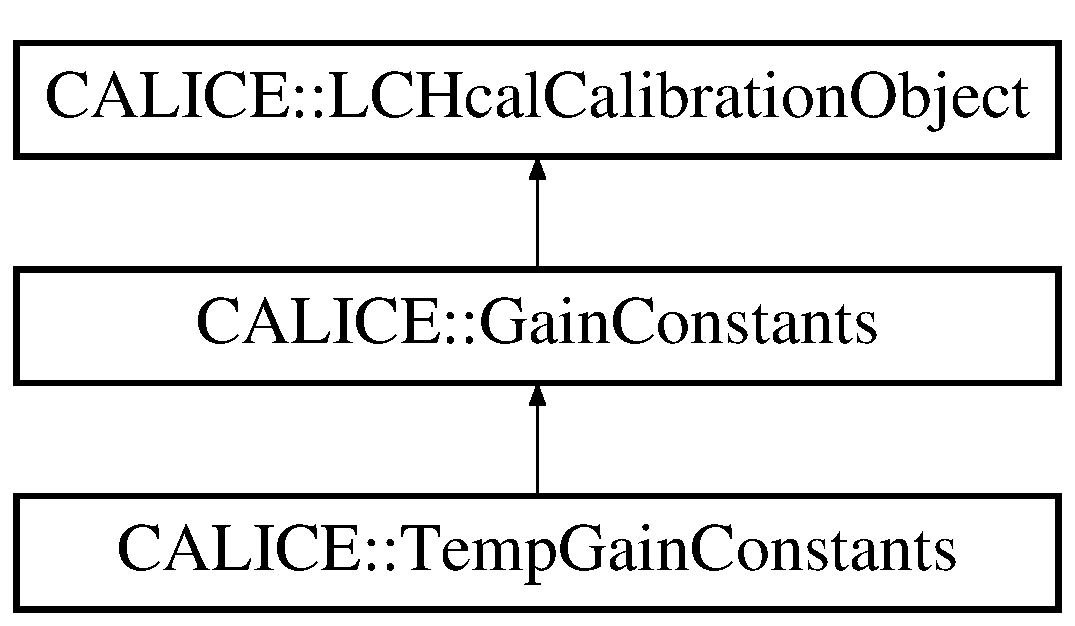
\includegraphics[height=3cm]{classCALICE_1_1GainConstants}
\end{center}
\end{figure}
\subsection*{Public Member Functions}
\begin{DoxyCompactItemize}
\item 
{\bf GainConstants} ()\label{classCALICE_1_1GainConstants_a39dd2a091779511dace0357560720578}

\begin{DoxyCompactList}\small\item\em contructor \item\end{DoxyCompactList}\item 
{\bf GainConstants} (unsigned chip, unsigned channel, float value, float error)
\begin{DoxyCompactList}\small\item\em constructor, initialised by parameters \item\end{DoxyCompactList}\item 
{\bfseries GainConstants} (LCObject $\ast$obj)\label{classCALICE_1_1GainConstants_ac092d7226de27568f20cdf941048eab8}

\item 
float {\bf getGainValue} () const \label{classCALICE_1_1GainConstants_a77246e61085596f25500286de31b9701}

\begin{DoxyCompactList}\small\item\em get channels/pixel value \item\end{DoxyCompactList}\item 
float {\bf getGainError} () const \label{classCALICE_1_1GainConstants_a85df3d26a093d548f2ae72f161be9882}

\begin{DoxyCompactList}\small\item\em get channels/pixel error \item\end{DoxyCompactList}\item 
float {\bf applyCalibration} (float inputValue) const 
\begin{DoxyCompactList}\small\item\em apply gain calibration to energy value \item\end{DoxyCompactList}\item 
float {\bf cancelCalibration} (float outputValue) const \label{classCALICE_1_1GainConstants_a320f0ebbbfb5973adb079fcee0b75d68}

\begin{DoxyCompactList}\small\item\em cancel an applied calibration from energy value \item\end{DoxyCompactList}\item 
float {\bf applyCalibrationError} (float inputValue, float inputError) const 
\begin{DoxyCompactList}\small\item\em apply calibration error to current error \item\end{DoxyCompactList}\item 
float {\bf cancelCalibrationError} (float outputValue, float outputError) const \label{classCALICE_1_1GainConstants_ab9ad1c0318937d2ad4d1cde2564e21e6}

\begin{DoxyCompactList}\small\item\em apply error due to canceling a calibration to current error \item\end{DoxyCompactList}\item 
bool {\bf calibrationValid} () const 
\begin{DoxyCompactList}\small\item\em check if a valid gain calibration is available \item\end{DoxyCompactList}\item 
bool {\bf keepEvent} (float resultValue, float resultError) const 
\begin{DoxyCompactList}\small\item\em no cut for the moment \item\end{DoxyCompactList}\item 
void {\bf print} (std::ostream \&os)\label{classCALICE_1_1GainConstants_aadeeb578a162265a5303b15e8f0dc50c}

\begin{DoxyCompactList}\small\item\em convenient print method \item\end{DoxyCompactList}\item 
const std::string {\bf getTypeName} () const \label{classCALICE_1_1GainConstants_af434ce23496e1b3d56967c87de010358}

\begin{DoxyCompactList}\small\item\em return type of the class \item\end{DoxyCompactList}\item 
const std::string {\bf getDataDescription} () const \label{classCALICE_1_1GainConstants_a3d8dec743df6d2d334e0ab6e3bc52e00}

\begin{DoxyCompactList}\small\item\em return a brief description of the data member \item\end{DoxyCompactList}\end{DoxyCompactItemize}


\subsection{Detailed Description}
Class to store the results of a Gain calibration measurement, i.e. gain plus the error of it for a certain chip/channel for a fixed moduleID \begin{DoxyAuthor}{Author}
S. Schmidt DESY 
\end{DoxyAuthor}
\begin{DoxyDate}{Date}
Aug 18 2006 
\end{DoxyDate}


Definition at line 25 of file GainConstants.hh.

\subsection{Constructor \& Destructor Documentation}
\index{CALICE::GainConstants@{CALICE::GainConstants}!GainConstants@{GainConstants}}
\index{GainConstants@{GainConstants}!CALICE::GainConstants@{CALICE::GainConstants}}
\subsubsection[{GainConstants}]{\setlength{\rightskip}{0pt plus 5cm}CALICE::GainConstants::GainConstants (unsigned {\em chip}, \/  unsigned {\em channel}, \/  float {\em value}, \/  float {\em error})\hspace{0.3cm}{\ttfamily  [inline]}}\label{classCALICE_1_1GainConstants_aa54fb6fbbf660c2ccb43ab9eaa8ef63c}


constructor, initialised by parameters 
\begin{DoxyParams}{Parameters}
\item[{\em chip}]chip number of the cell to be calibrated \item[{\em channel}]channel number of the cell to be calibrated \item[{\em value}]gain value \item[{\em error}]error on the gain value \end{DoxyParams}


Definition at line 39 of file GainConstants.hh.

References CALICE::LCHcalCalibrationObject::obj(), and CALICE::LCHcalCalibrationObject::setCellKey().

\subsection{Member Function Documentation}
\index{CALICE::GainConstants@{CALICE::GainConstants}!applyCalibration@{applyCalibration}}
\index{applyCalibration@{applyCalibration}!CALICE::GainConstants@{CALICE::GainConstants}}
\subsubsection[{applyCalibration}]{\setlength{\rightskip}{0pt plus 5cm}float CALICE::GainConstants::applyCalibration (float {\em inputValue}) const\hspace{0.3cm}{\ttfamily  [inline, virtual]}}\label{classCALICE_1_1GainConstants_aeb089dc140f6e63d2f0a4746ecdd5cbb}


apply gain calibration to energy value 
\begin{DoxyParams}{Parameters}
\item[{\em inputValue}]\char`\"{}energy\char`\"{} value before the gain calibration \end{DoxyParams}
\begin{DoxyReturn}{Returns}
\char`\"{}energy\char`\"{} value after the gain calibration 
\end{DoxyReturn}


Reimplemented from {\bf CALICE::LCHcalCalibrationObject} \doxyref{}{p.}{classCALICE_1_1LCHcalCalibrationObject_a763f1cf5b9c372fdde268d79b789adcc}.

Reimplemented in {\bf CALICE::TempGainConstants} \doxyref{}{p.}{classCALICE_1_1TempGainConstants_ae2278e77d19368d5fb1ec5fb1eecef44}.

Definition at line 66 of file GainConstants.hh.

References getGainValue().\index{CALICE::GainConstants@{CALICE::GainConstants}!applyCalibrationError@{applyCalibrationError}}
\index{applyCalibrationError@{applyCalibrationError}!CALICE::GainConstants@{CALICE::GainConstants}}
\subsubsection[{applyCalibrationError}]{\setlength{\rightskip}{0pt plus 5cm}float CALICE::GainConstants::applyCalibrationError (float {\em inputValue}, \/  float {\em inputError}) const\hspace{0.3cm}{\ttfamily  [inline, virtual]}}\label{classCALICE_1_1GainConstants_a669886b01357faa0b2173384be3a60d3}


apply calibration error to current error 
\begin{DoxyParams}{Parameters}
\item[{\em inputValue}]\char`\"{}energy\char`\"{} value before the gain calibration \item[{\em inputError}]error on the \char`\"{}energy\char`\"{} value before the gain calibration \end{DoxyParams}
\begin{DoxyReturn}{Returns}
error of the \char`\"{}energy\char`\"{} value after the calibration, gained from error propagation of the error of the \char`\"{}energy\char`\"{} value before the calibration and the error of the gain calibration 
\end{DoxyReturn}


Reimplemented from {\bf CALICE::LCHcalCalibrationObject} \doxyref{}{p.}{classCALICE_1_1LCHcalCalibrationObject_a16d9de9567f68d7784a2daa4d2821341}.

Reimplemented in {\bf CALICE::TempGainConstants} \doxyref{}{p.}{classCALICE_1_1TempGainConstants_a4319810d19fd6bb61de44faec1f56226}.

Definition at line 82 of file GainConstants.hh.

References getGainError(), and getGainValue().\index{CALICE::GainConstants@{CALICE::GainConstants}!calibrationValid@{calibrationValid}}
\index{calibrationValid@{calibrationValid}!CALICE::GainConstants@{CALICE::GainConstants}}
\subsubsection[{calibrationValid}]{\setlength{\rightskip}{0pt plus 5cm}bool CALICE::GainConstants::calibrationValid () const\hspace{0.3cm}{\ttfamily  [inline, virtual]}}\label{classCALICE_1_1GainConstants_a37c5d66f2537eee42e259147856e86a7}


check if a valid gain calibration is available \begin{DoxyReturn}{Returns}
true if the gain value is a valid number 
\end{DoxyReturn}


Reimplemented from {\bf CALICE::LCHcalCalibrationObject} \doxyref{}{p.}{classCALICE_1_1LCHcalCalibrationObject_abbb1fce81f41a89147b721d593bbc734}.

Reimplemented in {\bf CALICE::TempGainConstants} \doxyref{}{p.}{classCALICE_1_1TempGainConstants_a132d04dd01b328d85857bda95baf000b}.

Definition at line 95 of file GainConstants.hh.

References getGainValue().

Referenced by CALICE::TempGainConstants::calibrationValid().\index{CALICE::GainConstants@{CALICE::GainConstants}!keepEvent@{keepEvent}}
\index{keepEvent@{keepEvent}!CALICE::GainConstants@{CALICE::GainConstants}}
\subsubsection[{keepEvent}]{\setlength{\rightskip}{0pt plus 5cm}bool CALICE::GainConstants::keepEvent (float {\em resultValue}, \/  float {\em resultError}) const\hspace{0.3cm}{\ttfamily  [inline, virtual]}}\label{classCALICE_1_1GainConstants_a18c349f2f60b6f2d5d387fe386c63ebc}


no cut for the moment \begin{DoxyReturn}{Returns}
true, as no cut on cell level is performed after applying the gain calibration 
\end{DoxyReturn}


Reimplemented from {\bf CALICE::LCHcalCalibrationObject} \doxyref{}{p.}{classCALICE_1_1LCHcalCalibrationObject_a59f14a6b83e77717751ae4e7213e8d09}.

Definition at line 102 of file GainConstants.hh.

The documentation for this class was generated from the following files:\begin{DoxyCompactItemize}
\item 
GainConstants.hh\item 
GainConstants.cc\end{DoxyCompactItemize}

\section{CALICE::HcalBoardsConn Class Reference}
\label{classCALICE_1_1HcalBoardsConn}\index{CALICE::HcalBoardsConn@{CALICE::HcalBoardsConn}}


Mapping class based on the LCFixedObject template.  


{\ttfamily \#include $<$HcalBoardsConn.hh$>$}\subsection*{Public Member Functions}
\begin{DoxyCompactItemize}
\item 
{\bf HcalBoardsConn} (int connector\_\-pin, string hbab, string hab, int asic\_\-input, int analog\_\-output)\label{classCALICE_1_1HcalBoardsConn_a7382749f913df259e270ed363834ee57}

\begin{DoxyCompactList}\small\item\em Convenient c'tor. \item\end{DoxyCompactList}\item 
{\bf HcalBoardsConn} (LCObject $\ast$obj)\label{classCALICE_1_1HcalBoardsConn_a655bb16a946826a22f06e3da8ffc01f9}

\begin{DoxyCompactList}\small\item\em 'Copy constructor' needed to interpret LCCollection read from file/database. \item\end{DoxyCompactList}\item 
virtual {\bf $\sim$HcalBoardsConn} ()\label{classCALICE_1_1HcalBoardsConn_a73194f9ac5e8d51a886fb58943e07c65}

\begin{DoxyCompactList}\small\item\em Important for memory handling. \item\end{DoxyCompactList}\item 
int {\bf getConnectorPin} ()\label{classCALICE_1_1HcalBoardsConn_a682d3a3c73075248076bad7eb4608e34}

\begin{DoxyCompactList}\small\item\em the class interface: \item\end{DoxyCompactList}\item 
string {\bfseries getHbabID} ()\label{classCALICE_1_1HcalBoardsConn_a3cb9ccfe9aa2ab2a316d1d3c3ea5522b}

\item 
int {\bfseries getHabID} ()\label{classCALICE_1_1HcalBoardsConn_aaf33d239016770e85e88ba21af844404}

\item 
int {\bfseries getAsicInput} ()\label{classCALICE_1_1HcalBoardsConn_aa98763cad817a0d7e2dadf6b6ce249fa}

\item 
int {\bfseries getAnalogOutput} ()\label{classCALICE_1_1HcalBoardsConn_a69ecad7ef5cfb47baa7f8abed28b4145}

\item 
void {\bfseries print} (std::ostream \&os, std::string)\label{classCALICE_1_1HcalBoardsConn_abdd5c67e189a1a8e15399db9f81404e9}

\item 
const std::string {\bfseries getTypeName} () const \label{classCALICE_1_1HcalBoardsConn_afdf2f9b84e4c9477fa177fbfa0d2200f}

\item 
const std::string {\bfseries getDataDescription} () const \label{classCALICE_1_1HcalBoardsConn_af9c2280977a28e03c5b35f981304a841}

\end{DoxyCompactItemize}
\subsection*{Private Attributes}
\begin{DoxyCompactItemize}
\item 
short {\bfseries \_\-index}\label{classCALICE_1_1HcalBoardsConn_a2bd849016299c22be7a4d9848c4234c6}

\end{DoxyCompactItemize}


\subsection{Detailed Description}
Mapping class based on the LCFixedObject template. for principle Hcal boards connections \begin{DoxyAuthor}{Author}
R. P�schl DESY 
\end{DoxyAuthor}
\begin{DoxyDate}{Date}
May 005 
\end{DoxyDate}


Definition at line 30 of file HcalBoardsConn.hh.

The documentation for this class was generated from the following file:\begin{DoxyCompactItemize}
\item 
HcalBoardsConn.hh\end{DoxyCompactItemize}

\section{CALICE::HcalCassVsCrc Class Reference}
\label{classCALICE_1_1HcalCassVsCrc}\index{CALICE::HcalCassVsCrc@{CALICE::HcalCassVsCrc}}


Mapping class based on the LCFixedObject template that relates hcal-\/cassette $<$-\/$>$ crc board.  


{\ttfamily \#include $<$HcalCassVsCrc.hh$>$}\subsection*{Public Member Functions}
\begin{DoxyCompactItemize}
\item 
{\bf HcalCassVsCrc} (int cassetteID, int slotID, int feID)\label{classCALICE_1_1HcalCassVsCrc_acac3879060b6b68debe0a745edd6aee4}

\begin{DoxyCompactList}\small\item\em Convenient c'tor. \item\end{DoxyCompactList}\item 
{\bf HcalCassVsCrc} (LCObject $\ast$obj)\label{classCALICE_1_1HcalCassVsCrc_a8a358967f908bb95a3d91b1d146c29d5}

\begin{DoxyCompactList}\small\item\em 'Copy constructor' needed to interpret LCCollection read from file/database. \item\end{DoxyCompactList}\item 
virtual {\bf $\sim$HcalCassVsCrc} ()\label{classCALICE_1_1HcalCassVsCrc_a8a97f7c3778a20a0c5b07d7698ac1b98}

\begin{DoxyCompactList}\small\item\em Important for memory handling. \item\end{DoxyCompactList}\item 
int {\bf getCassetteID} ()\label{classCALICE_1_1HcalCassVsCrc_ad4aefc286108f1142bec4cf745a40688}

\begin{DoxyCompactList}\small\item\em the class interface: \item\end{DoxyCompactList}\item 
int {\bfseries getSlotID} ()\label{classCALICE_1_1HcalCassVsCrc_a369e980573265ca9b9db146b9e218ba3}

\item 
int {\bfseries getFeID} ()\label{classCALICE_1_1HcalCassVsCrc_a9fafc4450edc42942bc6e27400694709}

\item 
void {\bf print} (std::ostream \&os)\label{classCALICE_1_1HcalCassVsCrc_aff5276505cb70e00d8fd8da08a3bc340}

\begin{DoxyCompactList}\small\item\em convenient print function \item\end{DoxyCompactList}\item 
const std::string {\bfseries getTypeName} () const \label{classCALICE_1_1HcalCassVsCrc_a7e060dc4ae6b98c7881e8de228802932}

\item 
const std::string {\bfseries getDataDescription} () const \label{classCALICE_1_1HcalCassVsCrc_a70190ce23db321e7cd2ae283eb2c1f12}

\end{DoxyCompactItemize}


\subsection{Detailed Description}
Mapping class based on the LCFixedObject template that relates hcal-\/cassette $<$-\/$>$ crc board. 

Definition at line 28 of file HcalCassVsCrc.hh.

The documentation for this class was generated from the following files:\begin{DoxyCompactItemize}
\item 
HcalCassVsCrc.hh\item 
HcalCassVsCrc.cc\end{DoxyCompactItemize}

\section{CALICE::HcalCellIndex Class Reference}
\label{classCALICE_1_1HcalCellIndex}\index{CALICE::HcalCellIndex@{CALICE::HcalCellIndex}}


like \doxyref{CALICE::CellIndex}{p.}{classCALICE_1_1CellIndex}, but with HCAL related funciton names  


{\ttfamily \#include $<$HcalCellIndex.hh$>$}Inheritance diagram for CALICE::HcalCellIndex::\begin{figure}[H]
\begin{center}
\leavevmode
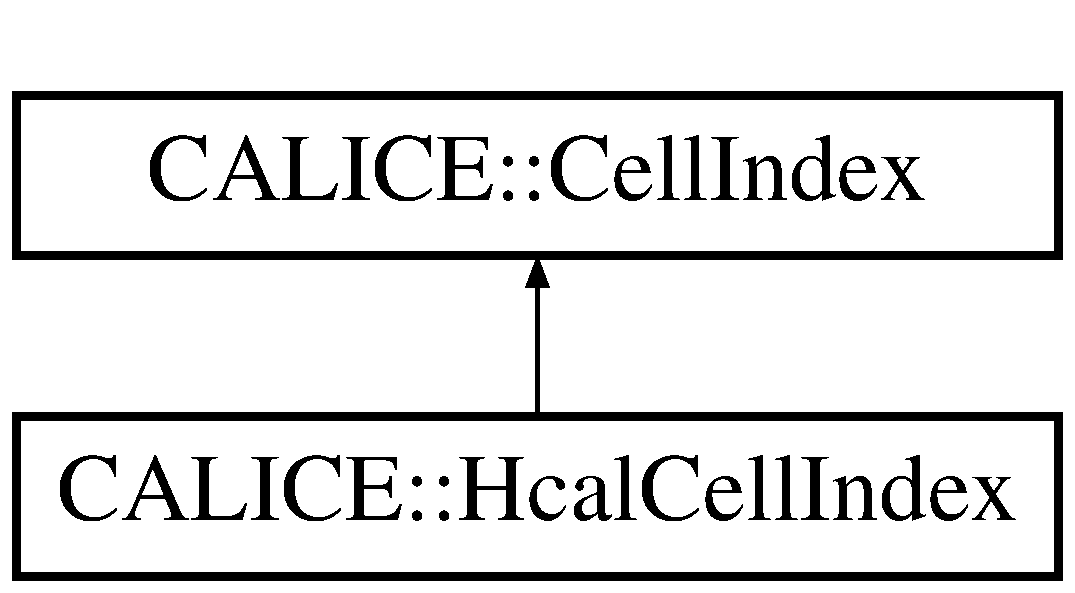
\includegraphics[height=2cm]{classCALICE_1_1HcalCellIndex}
\end{center}
\end{figure}
\subsection*{Public Member Functions}
\begin{DoxyCompactItemize}
\item 
{\bfseries HcalCellIndex} (UInt\_\-t pad\_\-row, UInt\_\-t pad\_\-column, UInt\_\-t layer)\label{classCALICE_1_1HcalCellIndex_abd7f2cb040e3699f5ec38624e1a01107}

\item 
{\bfseries HcalCellIndex} (UInt\_\-t geometrical\_\-cell\_\-index)\label{classCALICE_1_1HcalCellIndex_afa312d18c1d3a443bdd532b34a651346}

\item 
UInt\_\-t {\bf getTileRow} () const \label{classCALICE_1_1HcalCellIndex_a3dc148ed4fda61ef69e7fcc98f4f12fa}

\begin{DoxyCompactList}\small\item\em Get the tile row (index labeled J in Mokka). \item\end{DoxyCompactList}\item 
{\bf HcalCellIndex} \& {\bf setTileRow} (UInt\_\-t tile\_\-row)\label{classCALICE_1_1HcalCellIndex_a9771c1f35428728308129eb8bc1818b4}

\begin{DoxyCompactList}\small\item\em Set the tile row (index labeled J in Mokka). \item\end{DoxyCompactList}\item 
UInt\_\-t {\bf getTileColumn} () const \label{classCALICE_1_1HcalCellIndex_abb5872c8546b2aecb98e6c51bfb5d4a0}

\begin{DoxyCompactList}\small\item\em Get the tile column (index labeled I in Mokka). \item\end{DoxyCompactList}\item 
{\bf HcalCellIndex} \& {\bf setTileColumn} (UInt\_\-t tile\_\-column)\label{classCALICE_1_1HcalCellIndex_aed0ed386586f81b4b42f275a1837f876}

\begin{DoxyCompactList}\small\item\em Set the tile column (index labeled I in Mokka). \item\end{DoxyCompactList}\end{DoxyCompactItemize}
\subsection*{Static Public Member Functions}
\begin{DoxyCompactItemize}
\item 
static std::string {\bf getEncodingString} (const unsigned int startbit)\label{classCALICE_1_1HcalCellIndex_a67b7ed9d9984894fe1ec15372fc8016b}

\begin{DoxyCompactList}\small\item\em Return the cellid encoding string according to an lcio BitField64. \item\end{DoxyCompactList}\end{DoxyCompactItemize}


\subsection{Detailed Description}
like \doxyref{CALICE::CellIndex}{p.}{classCALICE_1_1CellIndex}, but with HCAL related funciton names \begin{DoxySeeAlso}{See also}
\doxyref{CALICE::CellIndex}{p.}{classCALICE_1_1CellIndex} 
\end{DoxySeeAlso}


Definition at line 27 of file HcalCellIndex.hh.

The documentation for this class was generated from the following file:\begin{DoxyCompactItemize}
\item 
HcalCellIndex.hh\end{DoxyCompactItemize}

\section{CALICE::HcalModuleIndexReverseLookup Class Reference}
\label{classCALICE_1_1HcalModuleIndexReverseLookup}\index{CALICE::HcalModuleIndexReverseLookup@{CALICE::HcalModuleIndexReverseLookup}}


Class to simplify the lookup geometrical index to hardware index.  


{\ttfamily \#include $<$HcalModuleIndexReverseLookup.hh$>$}\subsection*{Public Member Functions}
\begin{DoxyCompactItemize}
\item 
void {\bfseries createIndexReverseLookup} (const {\bf MappingAndAlignment} \&mapping)\label{classCALICE_1_1HcalModuleIndexReverseLookup_a03bfcfc65304f8f75efd7108c39cd7ee}

\item 
pair$<$ UInt\_\-t, UInt\_\-t $>$ {\bfseries getModuleAndCellIndex} (const {\bf MappingAndAlignment} \&mapping, const {\bf HcalCellIndex} \&a\_\-cell\_\-index) const \label{classCALICE_1_1HcalModuleIndexReverseLookup_a1e5edb46e871ee9ac4b260385de6282d}

\end{DoxyCompactItemize}
\subsection*{Protected Types}
\begin{DoxyCompactItemize}
\item 
typedef {\bf SimpleArray\_\-t}$<$ {\bf SimpleArray\_\-t}$<$ unsigned short $>$ $>$ {\bfseries CellIndexArray\_\-t}\label{classCALICE_1_1HcalModuleIndexReverseLookup_acfe7ef8150b7fc889aee587be5a9ff95}

\end{DoxyCompactItemize}
\subsection*{Protected Attributes}
\begin{DoxyCompactItemize}
\item 
{\bf SimpleArray\_\-t}$<$ {\bf CellIndexArray\_\-t} $>$ {\bf \_\-cellIndexArray}
\begin{DoxyCompactList}\small\item\em Array which contains for each cell the cell indices for pad row and column. \item\end{DoxyCompactList}\end{DoxyCompactItemize}


\subsection{Detailed Description}
Class to simplify the lookup geometrical index to hardware index. \begin{DoxyAuthor}{Author}
(probably) Sebastian Schmidt 
\end{DoxyAuthor}


Definition at line 12 of file HcalModuleIndexReverseLookup.hh.

\subsection{Field Documentation}
\index{CALICE::HcalModuleIndexReverseLookup@{CALICE::HcalModuleIndexReverseLookup}!\_\-cellIndexArray@{\_\-cellIndexArray}}
\index{\_\-cellIndexArray@{\_\-cellIndexArray}!CALICE::HcalModuleIndexReverseLookup@{CALICE::HcalModuleIndexReverseLookup}}
\subsubsection[{\_\-cellIndexArray}]{\setlength{\rightskip}{0pt plus 5cm}{\bf SimpleArray\_\-t}$<$ {\bf CellIndexArray\_\-t} $>$ {\bf CALICE::HcalModuleIndexReverseLookup::\_\-cellIndexArray}\hspace{0.3cm}{\ttfamily  [protected]}}\label{classCALICE_1_1HcalModuleIndexReverseLookup_a28b33f49d28d85e2fed000e524429e24}


Array which contains for each cell the cell indices for pad row and column. 

Definition at line 35 of file HcalModuleIndexReverseLookup.hh.

The documentation for this class was generated from the following files:\begin{DoxyCompactItemize}
\item 
HcalModuleIndexReverseLookup.hh\item 
HcalModuleIndexReverseLookup.cc\end{DoxyCompactItemize}

\section{CALICE::HcalTileIndex Class Reference}
\label{classCALICE_1_1HcalTileIndex}\index{CALICE::HcalTileIndex@{CALICE::HcalTileIndex}}


Encodes/decodes hardware channel information for the \doxyref{CALICE}{p.}{namespaceCALICE} AHCAL prototype.  


{\ttfamily \#include $<$HcalTileIndex.hh$>$}\subsection*{Public Member Functions}
\begin{DoxyCompactItemize}
\item 
{\bf HcalTileIndex} ()
\begin{DoxyCompactList}\small\item\em Empty constructor. \item\end{DoxyCompactList}\item 
{\bf HcalTileIndex} (int index)\label{classCALICE_1_1HcalTileIndex_a0aa6c6fdae8c031ff1f83dd8efe9c6d6}

\begin{DoxyCompactList}\small\item\em Constructor from an integer for decoding. \item\end{DoxyCompactList}\item 
{\bf HcalTileIndex} (short mod, short chip, short chan)
\begin{DoxyCompactList}\small\item\em Constructor from the minimum set of parameters required for unique identification. \item\end{DoxyCompactList}\item 
{\bf HcalTileIndex} (short mod, short chip, short chan, short sipm)
\begin{DoxyCompactList}\small\item\em Constructor from the full set of parameters. \item\end{DoxyCompactList}\item 
{\bf $\sim$HcalTileIndex} ()\label{classCALICE_1_1HcalTileIndex_a398e94753c897c5d34d88b3401f5fd71}

\begin{DoxyCompactList}\small\item\em Destructor -\/ does nothing. \item\end{DoxyCompactList}\item 
unsigned short {\bf getModule} () const \label{classCALICE_1_1HcalTileIndex_a540b5492b1be53b703add6f02a2fed75}

\begin{DoxyCompactList}\small\item\em Decode module identifier. \item\end{DoxyCompactList}\item 
unsigned short {\bf getModuleType} () const \label{classCALICE_1_1HcalTileIndex_ad83da5fc1e46cb351b544ff9b4ed29b0}

\begin{DoxyCompactList}\small\item\em Derive module type from module and chip identifier. \item\end{DoxyCompactList}\item 
unsigned short {\bf getChip} () const \label{classCALICE_1_1HcalTileIndex_a0f64142ad01b7fef95ee8ee92727b9b7}

\begin{DoxyCompactList}\small\item\em Decode ASIC identifier. \item\end{DoxyCompactList}\item 
unsigned short {\bf getChannel} () const \label{classCALICE_1_1HcalTileIndex_a479e6ce42ffabcc633fb613ac01345fa}

\begin{DoxyCompactList}\small\item\em Decode multiplex channel. \item\end{DoxyCompactList}\item 
unsigned short {\bf getSipm} () const \label{classCALICE_1_1HcalTileIndex_ab488979a06db1ca13cdccbd43adc9308}

\begin{DoxyCompactList}\small\item\em Decode SiPM number. \item\end{DoxyCompactList}\item 
unsigned int {\bf getIndex} () const \label{classCALICE_1_1HcalTileIndex_a29c1878383ea8593073db1478f3f1baf}

\begin{DoxyCompactList}\small\item\em Return THE index. \item\end{DoxyCompactList}\item 
{\bf HcalTileIndex} \& {\bf setModule} (short mod)\label{classCALICE_1_1HcalTileIndex_a1194d53c0179b3dd2a6c5e03ec9a0524}

\begin{DoxyCompactList}\small\item\em Encode module identifier. \item\end{DoxyCompactList}\item 
{\bf HcalTileIndex} \& {\bf setChip} (short chip)\label{classCALICE_1_1HcalTileIndex_ab2e3d8ecf1c8e623b45433c2742c6ca8}

\begin{DoxyCompactList}\small\item\em Encode ASIC identifier. \item\end{DoxyCompactList}\item 
{\bf HcalTileIndex} \& {\bf setChannel} (short chan)\label{classCALICE_1_1HcalTileIndex_a4f45965bc383f021d06a020d37f85799}

\begin{DoxyCompactList}\small\item\em Encode multiplex channel. \item\end{DoxyCompactList}\item 
{\bf HcalTileIndex} \& {\bf setSipm} (short sipm)\label{classCALICE_1_1HcalTileIndex_a1fb54613eea3444cd8308d742f78875c}

\begin{DoxyCompactList}\small\item\em Encode SiPM number. \item\end{DoxyCompactList}\end{DoxyCompactItemize}
\subsection*{Static Public Member Functions}
\begin{DoxyCompactItemize}
\item 
static std::string {\bf getEncodingString} (const unsigned int startbit)\label{classCALICE_1_1HcalTileIndex_a869cd817ebbb8d5b542e7cfa61bd62f0}

\begin{DoxyCompactList}\small\item\em Return the cellid encoding string according to an lcio BitField64. \item\end{DoxyCompactList}\end{DoxyCompactItemize}
\subsection*{Protected Attributes}
\begin{DoxyCompactItemize}
\item 
unsigned int {\bfseries \_\-index}\label{classCALICE_1_1HcalTileIndex_aee8c8f51535723b3746d75ce49e54a81}

\end{DoxyCompactItemize}


\subsection{Detailed Description}
Encodes/decodes hardware channel information for the \doxyref{CALICE}{p.}{namespaceCALICE} AHCAL prototype. This class encodes and decodes module, chip and channel as well as the SiPM number into/from a single integer. This integer is intended to be stored in the CellID1 field of LCIO CalorimeterHit objects for easy reference to and unique identification of the hardware information of reconstructed hits.

\begin{DoxyAuthor}{Author}
{\tt Niels.Meyer@desy.de} 
\end{DoxyAuthor}
\begin{DoxyDate}{Date}
Nov. 17, 2007 
\end{DoxyDate}
\begin{DoxyVersion}{Version}
1.0 
\end{DoxyVersion}


Definition at line 39 of file HcalTileIndex.hh.

\subsection{Constructor \& Destructor Documentation}
\index{CALICE::HcalTileIndex@{CALICE::HcalTileIndex}!HcalTileIndex@{HcalTileIndex}}
\index{HcalTileIndex@{HcalTileIndex}!CALICE::HcalTileIndex@{CALICE::HcalTileIndex}}
\subsubsection[{HcalTileIndex}]{\setlength{\rightskip}{0pt plus 5cm}CALICE::HcalTileIndex::HcalTileIndex ()\hspace{0.3cm}{\ttfamily  [inline]}}\label{classCALICE_1_1HcalTileIndex_a50664f3b0b2355edd5cd99d04005477d}


Empty constructor. All parameters default to zero. 

Definition at line 43 of file HcalTileIndex.hh.

References setChannel(), setChip(), setModule(), and setSipm().\index{CALICE::HcalTileIndex@{CALICE::HcalTileIndex}!HcalTileIndex@{HcalTileIndex}}
\index{HcalTileIndex@{HcalTileIndex}!CALICE::HcalTileIndex@{CALICE::HcalTileIndex}}
\subsubsection[{HcalTileIndex}]{\setlength{\rightskip}{0pt plus 5cm}CALICE::HcalTileIndex::HcalTileIndex (short {\em mod}, \/  short {\em chip}, \/  short {\em chan})\hspace{0.3cm}{\ttfamily  [inline]}}\label{classCALICE_1_1HcalTileIndex_aad5b0d551d3733fabf0d9e086dfe5794}


Constructor from the minimum set of parameters required for unique identification. The SiPM number defaults to zero.


\begin{DoxyParams}{Parameters}
\item[{\em mod}]Module identifier \item[{\em chip}]ASIC chip identifier \item[{\em chan}]Multiplex channel identifier \end{DoxyParams}


Definition at line 60 of file HcalTileIndex.hh.

References setChannel(), setChip(), setModule(), and setSipm().\index{CALICE::HcalTileIndex@{CALICE::HcalTileIndex}!HcalTileIndex@{HcalTileIndex}}
\index{HcalTileIndex@{HcalTileIndex}!CALICE::HcalTileIndex@{CALICE::HcalTileIndex}}
\subsubsection[{HcalTileIndex}]{\setlength{\rightskip}{0pt plus 5cm}CALICE::HcalTileIndex::HcalTileIndex (short {\em mod}, \/  short {\em chip}, \/  short {\em chan}, \/  short {\em sipm})\hspace{0.3cm}{\ttfamily  [inline]}}\label{classCALICE_1_1HcalTileIndex_a0bfbc207ddb962b86ab31991b504645b}


Constructor from the full set of parameters. 
\begin{DoxyParams}{Parameters}
\item[{\em mod}]Module identifier \item[{\em chip}]ASIC chip identifier \item[{\em chan}]Multiplex channel identifier \item[{\em sipm}]SiPM identifier \end{DoxyParams}


Definition at line 71 of file HcalTileIndex.hh.

References setChannel(), setChip(), setModule(), and setSipm().

The documentation for this class was generated from the following file:\begin{DoxyCompactItemize}
\item 
HcalTileIndex.hh\end{DoxyCompactItemize}

\section{CALICE::HodoscopeEventDataBlock Class Reference}
\label{classCALICE_1_1HodoscopeEventDataBlock}\index{CALICE::HodoscopeEventDataBlock@{CALICE::HodoscopeEventDataBlock}}


Interface class to the (LAL) Hodoscope data.  


{\ttfamily \#include $<$HodoscopeEventDataBlock.hh$>$}Inheritance diagram for CALICE::HodoscopeEventDataBlock::\begin{figure}[H]
\begin{center}
\leavevmode
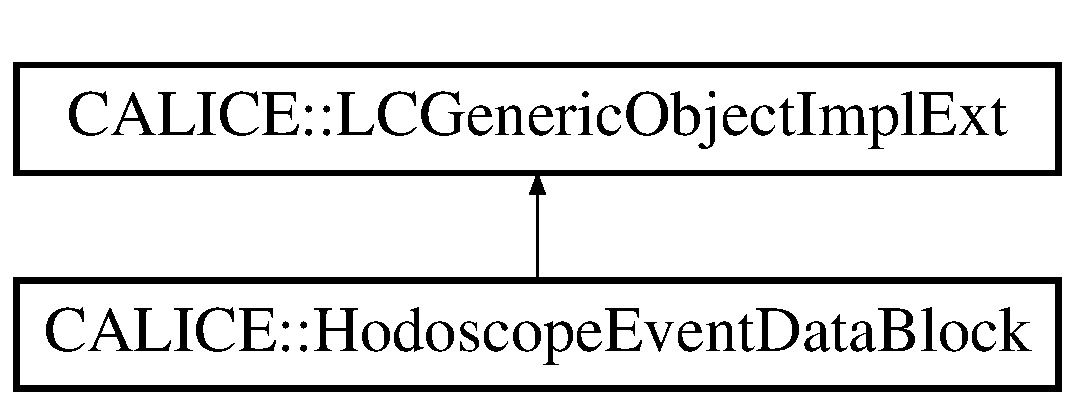
\includegraphics[height=2cm]{classCALICE_1_1HodoscopeEventDataBlock}
\end{center}
\end{figure}
\subsection*{Public Member Functions}
\begin{DoxyCompactItemize}
\item 
{\bf HodoscopeEventDataBlock} ()\label{classCALICE_1_1HodoscopeEventDataBlock_a737bf8e239af349eee5ff61472f0d181}

\begin{DoxyCompactList}\small\item\em Default Constructor. \item\end{DoxyCompactList}\item 
{\bf HodoscopeEventDataBlock} (LCObject $\ast$obj)\label{classCALICE_1_1HodoscopeEventDataBlock_ab99ff6344343b01653080763d612294a}

\begin{DoxyCompactList}\small\item\em 'Copy constructor' needed to interpret LCCollection read from file/database. \item\end{DoxyCompactList}\item 
{\bf HodoscopeEventDataBlock} \& {\bfseries setStatusWord} (int status)\label{classCALICE_1_1HodoscopeEventDataBlock_a8c84a40787e11df246f568c9a71ceee3}

\item 
int {\bf getStatusWord} () const \label{classCALICE_1_1HodoscopeEventDataBlock_af60190fb30f52df3a5697322a8965381}

\begin{DoxyCompactList}\small\item\em Get the Hodoscope Status. \item\end{DoxyCompactList}\item 
{\bf HodoscopeEventDataBlock} \& {\bfseries setEventCounter} (int counter)\label{classCALICE_1_1HodoscopeEventDataBlock_aa900a9d896467976dd716c3bbab1f99f}

\item 
int {\bf getEventCounter} () const \label{classCALICE_1_1HodoscopeEventDataBlock_a76db2626be9c0cd318bcf1fd0fced760}

\begin{DoxyCompactList}\small\item\em Get the Event counter. \item\end{DoxyCompactList}\item 
{\bf HodoscopeEventDataBlock} \& {\bf setTimeCounter} (int timecounter)\label{classCALICE_1_1HodoscopeEventDataBlock_abb2c7d94d1148d184c54ae66e98c3be4}

\begin{DoxyCompactList}\small\item\em Set time counter. \item\end{DoxyCompactList}\item 
int {\bf getTimeCounter} () const \label{classCALICE_1_1HodoscopeEventDataBlock_a50fb6763875658f8b91a186ec470a2da}

\begin{DoxyCompactList}\small\item\em Get the time counter. \item\end{DoxyCompactList}\item 
void {\bfseries storeHitMaps} (std::vector$<$ int $>$ \&, std::vector$<$ int $>$ \&)\label{classCALICE_1_1HodoscopeEventDataBlock_af6847f3dc217a31f37d5e0a3be862248}

\item 
unsigned int {\bf getNumHitsX} () const \label{classCALICE_1_1HodoscopeEventDataBlock_a854a79d6e112dc7153809afbcb71e40c}

\begin{DoxyCompactList}\small\item\em Get the Number of Hits in X direction. \item\end{DoxyCompactList}\item 
unsigned int {\bf getNumHitsY} () const \label{classCALICE_1_1HodoscopeEventDataBlock_ae70c4a92cef77cc73726cd40ead186d3}

\begin{DoxyCompactList}\small\item\em Get the Number of Hits in Y direction. \item\end{DoxyCompactList}\item 
HodoscopeHitMap\_\-t {\bf getHitMapX} () const \label{classCALICE_1_1HodoscopeEventDataBlock_a56ff52ae20c90600f4268e2a9ec11015}

\begin{DoxyCompactList}\small\item\em Give the hit maps to the user. \item\end{DoxyCompactList}\item 
HodoscopeHitMap\_\-t {\bfseries getHitMapY} () const \label{classCALICE_1_1HodoscopeEventDataBlock_a536eb4acf8bebaa40022d7cc874779ee}

\item 
void {\bf print} (std::ostream \&os)\label{classCALICE_1_1HodoscopeEventDataBlock_aaeb17542763207334de0346c9c02f8c8}

\begin{DoxyCompactList}\small\item\em Convenient print method. \item\end{DoxyCompactList}\item 
const std::string {\bf getTypeName} () const \label{classCALICE_1_1HodoscopeEventDataBlock_a94f5e904602e4d9a4256c232a9e18068}

\begin{DoxyCompactList}\small\item\em Return the type of the class. \item\end{DoxyCompactList}\item 
const std::string {\bf getDataDescription} () const \label{classCALICE_1_1HodoscopeEventDataBlock_a736f44f539d1f896242cbc3682e32a79}

\begin{DoxyCompactList}\small\item\em Return a brief description of the data members. \item\end{DoxyCompactList}\end{DoxyCompactItemize}
\subsection*{Private Member Functions}
\begin{DoxyCompactItemize}
\item 
void {\bf createHitMaps} ()\label{classCALICE_1_1HodoscopeEventDataBlock_aa2133e011daaf804ee14b31f53084b69}

\begin{DoxyCompactList}\small\item\em A method to create the hitmaps (to be called by the constructor at access time. \item\end{DoxyCompactList}\end{DoxyCompactItemize}
\subsection*{Private Attributes}
\begin{DoxyCompactItemize}
\item 
HodoscopeHitMap\_\-t {\bf \_\-hitMapX}\label{classCALICE_1_1HodoscopeEventDataBlock_aca7b8496ec0403b0ac1dae0e137b6660}

\begin{DoxyCompactList}\small\item\em The hitmaps measured by the hodoscope. \item\end{DoxyCompactList}\item 
HodoscopeHitMap\_\-t {\bfseries \_\-hitMapY}\label{classCALICE_1_1HodoscopeEventDataBlock_a5e9c5d17dbc060cc176b3bf26c099a4d}

\item 
bool {\bf \_\-hitMapsCreated}\label{classCALICE_1_1HodoscopeEventDataBlock_a64ba1b45e7d59de63a972a762f976791}

\begin{DoxyCompactList}\small\item\em A pool which checks whetherthe hit map has already been recreated. \item\end{DoxyCompactList}\end{DoxyCompactItemize}


\subsection{Detailed Description}
Interface class to the (LAL) Hodoscope data. From the user point of view the class returns maps containing the hits in x and y respectively, but also other values like the timecounter and eventcounter are returned. The latter is useful to check whether the hodoscope has been in synch with the daq. \begin{DoxyAuthor}{Author}
R. Poeschl LAL (based on the other interface classes)
\end{DoxyAuthor}
\begin{DoxyDate}{Date}
Aug 2007 
\end{DoxyDate}


Definition at line 41 of file HodoscopeEventDataBlock.hh.

The documentation for this class was generated from the following files:\begin{DoxyCompactItemize}
\item 
HodoscopeEventDataBlock.hh\item 
HodoscopeEventDataBlock.cc\end{DoxyCompactItemize}

\section{HstBase Class Reference}
\label{classHstBase}\index{HstBase@{HstBase}}
Inheritance diagram for HstBase::\begin{figure}[H]
\begin{center}
\leavevmode
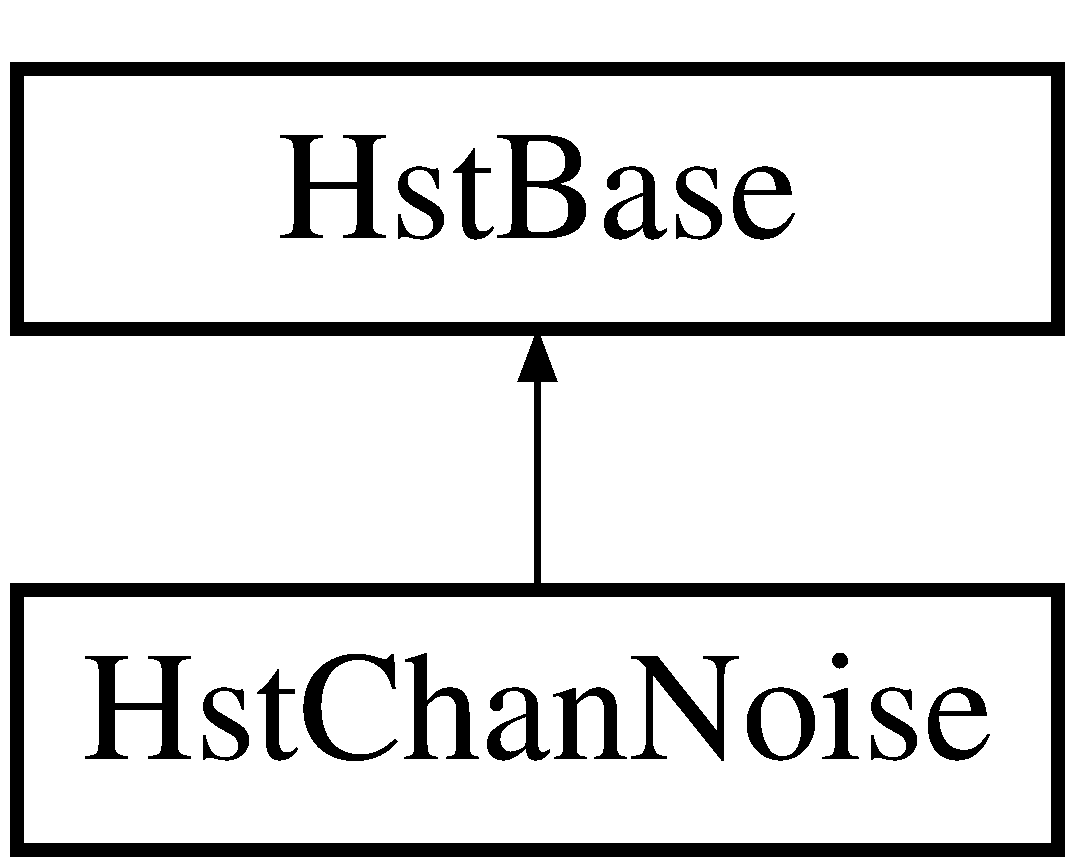
\includegraphics[height=2cm]{classHstBase}
\end{center}
\end{figure}
\subsection*{Public Member Functions}
\begin{DoxyCompactItemize}
\item 
{\bfseries HstBase} (bool i=true)\label{classHstBase_a36170c7c3f81997751b98e57773101ee}

\item 
virtual unsigned {\bfseries printLevel} () const \label{classHstBase_aa4f0acae99e23ea1cd2bd405259f14e2}

\item 
virtual void {\bfseries printLevel} (unsigned p)\label{classHstBase_ad125d12a8b12d0acf69da1dac0a9634c}

\item 
virtual bool {\bfseries record} (const RcdRecord \&r)=0\label{classHstBase_aedddcccf2663a04211ae01a44947d5ff}

\item 
virtual bool {\bfseries update} ()=0\label{classHstBase_a6b304127c3c6adc87ab30d1f9d4d557c}

\item 
virtual bool {\bfseries postscript} (std::string)=0\label{classHstBase_a88ed97ffe429ec2ca0d49faaf9a468ce}

\item 
bool {\bfseries interactive} () const \label{classHstBase_ac3297b878d90b6174577ef0f150cfb75}

\end{DoxyCompactItemize}
\subsection*{Private Attributes}
\begin{DoxyCompactItemize}
\item 
const bool {\bfseries \_\-interactive}\label{classHstBase_a65dd208a8144cd46de0a8c12497c5e02}

\item 
TApplication $\ast$ {\bfseries \_\-application}\label{classHstBase_a6d76a46a314f2c728bbea75f5cbb112c}

\item 
unsigned {\bfseries \_\-printLevel}\label{classHstBase_af08876ecbd5e3a7b238b94ef01aaea65}

\end{DoxyCompactItemize}


\subsection{Detailed Description}


Definition at line 12 of file HstBase.hh.

The documentation for this class was generated from the following file:\begin{DoxyCompactItemize}
\item 
HstBase.hh\end{DoxyCompactItemize}

\section{HstChanNoise Class Reference}
\label{classHstChanNoise}\index{HstChanNoise@{HstChanNoise}}
Inheritance diagram for HstChanNoise::\begin{figure}[H]
\begin{center}
\leavevmode
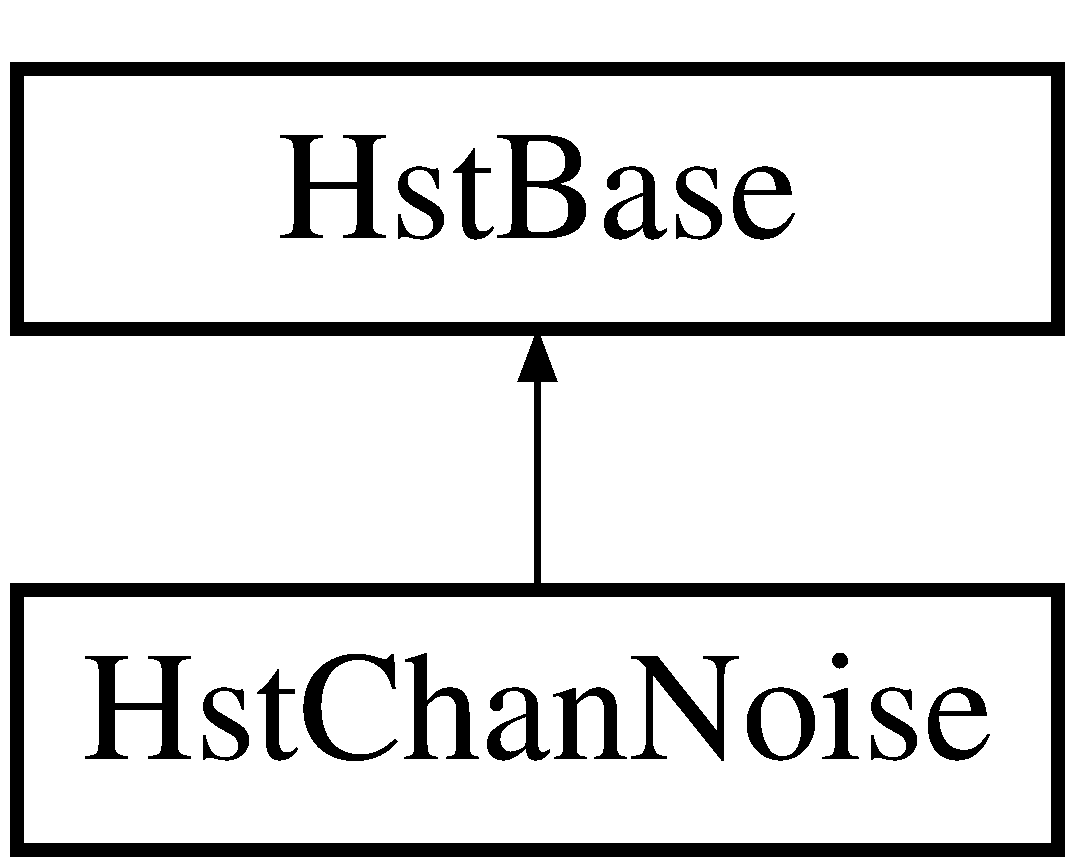
\includegraphics[height=2cm]{classHstChanNoise}
\end{center}
\end{figure}
\subsection*{Public Member Functions}
\begin{DoxyCompactItemize}
\item 
{\bfseries HstChanNoise} (bool i=true)\label{classHstChanNoise_a586bcb45dc76e29586a3f79bb59bbe8f}

\item 
void {\bfseries slotCanvas} (unsigned slot)\label{classHstChanNoise_a8fb12b44a7564921e59e1300ad8f7ab2}

\item 
bool {\bfseries postscript} (std::string)\label{classHstChanNoise_a2fab50c4976f17c718e7f9cb0ca1694a}

\item 
bool {\bfseries update} ()\label{classHstChanNoise_a33aecd229ce83bb779fc0dab34e80b8b}

\item 
bool {\bfseries record} (const RcdRecord \&r)\label{classHstChanNoise_a188b2650b4d8831ac6f5b0898afa3238}

\end{DoxyCompactItemize}
\subsection*{Private Attributes}
\begin{DoxyCompactItemize}
\item 
TCanvas $\ast$ {\bfseries \_\-canvas} [22]\label{classHstChanNoise_afca4c54c58f90144d08e96e5a713bb08}

\item 
{\bf HstTGraphErrors} {\bfseries \_\-graph} [22][2]\label{classHstChanNoise_aa8edb46e9f86b2d65e27733f43a97c56}

\item 
TH1D {\bfseries \_\-hist} [22][8][12][18]\label{classHstChanNoise_af5b44ba98a96215f69c9ea43b91609f0}

\item 
bool {\bfseries \_\-slot} [22]\label{classHstChanNoise_a3c3276da2e7ad7d8be0d68e4acdd58f9}

\item 
std::string {\bfseries \_\-label} [22]\label{classHstChanNoise_a2ed69a9688c335106a0695c001048592}

\item 
UtlAverage {\bfseries \_\-average} [22][8][12][18]\label{classHstChanNoise_a616ded317f4c23c9297c8474511515ef}

\end{DoxyCompactItemize}


\subsection{Detailed Description}


Definition at line 29 of file HstChanNoise.hh.

The documentation for this class was generated from the following file:\begin{DoxyCompactItemize}
\item 
HstChanNoise.hh\end{DoxyCompactItemize}

\section{HstTGraphErrors Class Reference}
\label{classHstTGraphErrors}\index{HstTGraphErrors@{HstTGraphErrors}}
\subsection*{Public Member Functions}
\begin{DoxyCompactItemize}
\item 
void {\bfseries AddPoint} (Double\_\-t x, Double\_\-t y, Double\_\-t ex, Double\_\-t ey)\label{classHstTGraphErrors_ae5c0b07b9beab247ae528aa467c98530}

\end{DoxyCompactItemize}


\subsection{Detailed Description}


Definition at line 7 of file HstTGraphErrors.hh.

The documentation for this class was generated from the following file:\begin{DoxyCompactItemize}
\item 
HstTGraphErrors.hh\end{DoxyCompactItemize}

\section{IConditionsChangeListener Class Reference}
\label{classlccd_1_1IConditionsChangeListener}\index{lccd::IConditionsChangeListener@{lccd::IConditionsChangeListener}}


Inherited by {\bf CALICE::ConditionsChangeDelegator$<$ TestCondDataProcessor $>$}, and {\bf CALICE::ConditionsChangeDelegator$<$ TriggerHandlerCalice $>$}.

The documentation for this class was generated from the following file:\begin{DoxyCompactItemize}
\item 
ConditionsChangeDelegator.hh\end{DoxyCompactItemize}

\section{CALICE::InterConstants Class Reference}
\label{classCALICE_1_1InterConstants}\index{CALICE::InterConstants@{CALICE::InterConstants}}


Class to store the results of a inter calibration measurement, i.e.  


{\ttfamily \#include $<$InterConstants.hh$>$}Inheritance diagram for CALICE::InterConstants::\begin{figure}[H]
\begin{center}
\leavevmode
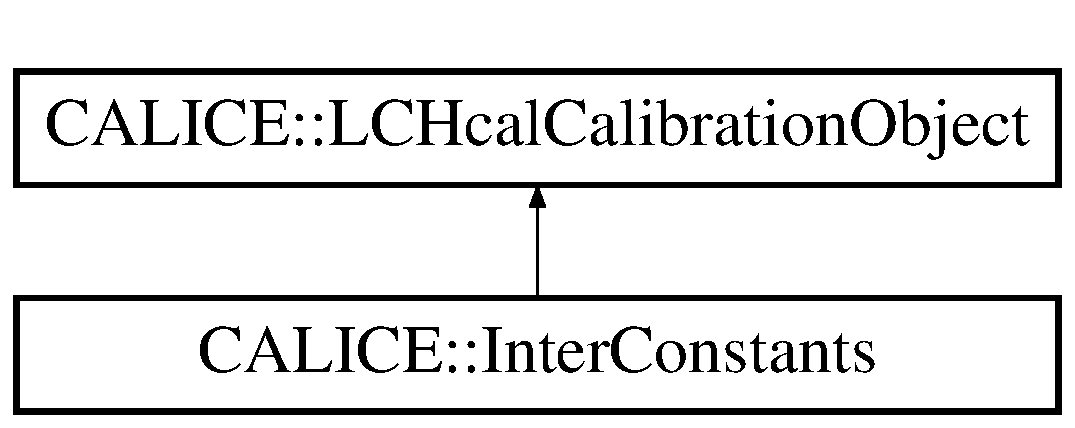
\includegraphics[height=2cm]{classCALICE_1_1InterConstants}
\end{center}
\end{figure}
\subsection*{Public Member Functions}
\begin{DoxyCompactItemize}
\item 
{\bfseries InterConstants} (unsigned chip, unsigned channel, float value, float error)\label{classCALICE_1_1InterConstants_a9130ab502198dc16813f62f591155900}

\item 
{\bfseries InterConstants} (LCObject $\ast$obj)\label{classCALICE_1_1InterConstants_a8275f0285c5080d4024de5557e0d0709}

\item 
float {\bf getInterValue} () const \label{classCALICE_1_1InterConstants_a2da8b23255795109983569198e70bfd7}

\begin{DoxyCompactList}\small\item\em get conversion factor value \item\end{DoxyCompactList}\item 
float {\bf getInterError} () const \label{classCALICE_1_1InterConstants_a17d72b981677ced2bc941119dcd19b2f}

\begin{DoxyCompactList}\small\item\em get conversion factor error \item\end{DoxyCompactList}\item 
float {\bf applyCalibration} (float inputValue) const \label{classCALICE_1_1InterConstants_ac4e54f423b0048db8e79b745a53a5209}

\begin{DoxyCompactList}\small\item\em apply calibration to energy value \item\end{DoxyCompactList}\item 
float {\bf cancelCalibration} (float outputValue) const \label{classCALICE_1_1InterConstants_a2f2d1a18b5136f7e2772d25629b4ccb2}

\begin{DoxyCompactList}\small\item\em cancel an applied calibration from energy value \item\end{DoxyCompactList}\item 
float {\bf applyCalibrationError} (float inputValue, float inputError) const \label{classCALICE_1_1InterConstants_ad102c242709f9229f3936d04bb356be7}

\begin{DoxyCompactList}\small\item\em apply calibration error to current error \item\end{DoxyCompactList}\item 
float {\bf cancelCalibrationError} (float outputValue, float outputError) const \label{classCALICE_1_1InterConstants_a513532d0848335a04f9a58c314ff32ee}

\begin{DoxyCompactList}\small\item\em apply error due to canceling a calibration to current error \item\end{DoxyCompactList}\item 
bool {\bf calibrationValid} () const \label{classCALICE_1_1InterConstants_ab184f4d15b941b5ac67474b02eaab138}

\begin{DoxyCompactList}\small\item\em check if a valid calibration is available \item\end{DoxyCompactList}\item 
bool {\bf keepEvent} (float resultValue, float resultError) const \label{classCALICE_1_1InterConstants_a919e037d3e03029486c2a3c9713e772a}

\begin{DoxyCompactList}\small\item\em no cut for the moment \item\end{DoxyCompactList}\item 
void {\bf print} (std::ostream \&os)\label{classCALICE_1_1InterConstants_a8e10cd6994b21d613a8bd5e00ac3fdec}

\begin{DoxyCompactList}\small\item\em convenient print method \item\end{DoxyCompactList}\item 
const std::string {\bf getTypeName} () const \label{classCALICE_1_1InterConstants_ab8640910bfa5d47de555ab6b5f2bb8d6}

\begin{DoxyCompactList}\small\item\em return type of the class \item\end{DoxyCompactList}\item 
const std::string {\bf getDataDescription} () const \label{classCALICE_1_1InterConstants_a7e992cec8e1b2c2e3914b9cb9e8c9c10}

\begin{DoxyCompactList}\small\item\em return a brief description of the data member \item\end{DoxyCompactList}\end{DoxyCompactItemize}


\subsection{Detailed Description}
Class to store the results of a inter calibration measurement, i.e. conversion factor between calibration mode and physics mode plus the error of it for a certain chip/channel for a fixed moduleID \begin{DoxyAuthor}{Author}
S. Schmidt DESY 
\end{DoxyAuthor}
\begin{DoxyDate}{Date}
Aug 24 2006 
\end{DoxyDate}


Definition at line 25 of file InterConstants.hh.

The documentation for this class was generated from the following files:\begin{DoxyCompactItemize}
\item 
InterConstants.hh\item 
InterConstants.cc\end{DoxyCompactItemize}

\section{CALICE::LabviewBlock2 Class Reference}
\label{classCALICE_1_1LabviewBlock2}\index{CALICE::LabviewBlock2@{CALICE::LabviewBlock2}}


Class for the Labview Data as acquired by the AHCAL Labview.  


{\ttfamily \#include $<$LabviewBlock2.hh$>$}\subsection*{Public Member Functions}
\begin{DoxyCompactItemize}
\item 
{\bf LabviewBlock2} (int CycleNr, int BunchXID, int ChipID, int EvtNr, int Channel, int TDC, int ADC, int HitBit, int GainBit)\label{classCALICE_1_1LabviewBlock2_aa409f51a0803d4ca5e6fe15204262118}

\begin{DoxyCompactList}\small\item\em Convenient c'tor. \item\end{DoxyCompactList}\item 
{\bf LabviewBlock2} (LCObject $\ast$obj)\label{classCALICE_1_1LabviewBlock2_acb5c7d7d0a0d9aecff3434f8b712745d}

\begin{DoxyCompactList}\small\item\em 'Copy constructor' needed to interpret LCCollection read from file/database. \item\end{DoxyCompactList}\item 
virtual {\bf $\sim$LabviewBlock2} ()\label{classCALICE_1_1LabviewBlock2_aabc7bc093f568a532a4cf7097a84fb99}

\begin{DoxyCompactList}\small\item\em Important for memory handling. \item\end{DoxyCompactList}\item 
int {\bf GetCycleNr} () const \label{classCALICE_1_1LabviewBlock2_aabd11e4b300c4a3644ff5fbbf513af36}

\begin{DoxyCompactList}\small\item\em get the CycleNr. \item\end{DoxyCompactList}\item 
int {\bf GetBunchXID} () const \label{classCALICE_1_1LabviewBlock2_ae25025f2f9bc95883c2d6b23d38ecc8e}

\begin{DoxyCompactList}\small\item\em get the BunchXID. \item\end{DoxyCompactList}\item 
int {\bf GetChipID} () const \label{classCALICE_1_1LabviewBlock2_a6e1e7613bbf370e6a0e11ef3896bb6f9}

\begin{DoxyCompactList}\small\item\em get the ChipID. \item\end{DoxyCompactList}\item 
int {\bf GetEvtNr} () const \label{classCALICE_1_1LabviewBlock2_a8d4a67989cad5bf504971abc612653cc}

\begin{DoxyCompactList}\small\item\em get the EvtNr. \item\end{DoxyCompactList}\item 
int {\bf GetChannel} () const \label{classCALICE_1_1LabviewBlock2_a9636e5feb9a0cba799067f7b2390d25b}

\begin{DoxyCompactList}\small\item\em get the Channel. \item\end{DoxyCompactList}\item 
int {\bf GetTDC} () const \label{classCALICE_1_1LabviewBlock2_a57d069ac572fbc56de3abfaaa007eb6e}

\begin{DoxyCompactList}\small\item\em get the TDC. \item\end{DoxyCompactList}\item 
int {\bf GetADC} () const \label{classCALICE_1_1LabviewBlock2_ab3d5c72af2f3fa8dd180afb091455dee}

\begin{DoxyCompactList}\small\item\em get the ADC. \item\end{DoxyCompactList}\item 
int {\bf GetHitBit} () const \label{classCALICE_1_1LabviewBlock2_a98de016fe2fa0639ca0cc82b1eecf97f}

\begin{DoxyCompactList}\small\item\em get the HitBit. \item\end{DoxyCompactList}\item 
int {\bf GetGainBit} () const \label{classCALICE_1_1LabviewBlock2_a08c27201d04e385c9be5709ce2fb9525}

\begin{DoxyCompactList}\small\item\em get the GainBit. \item\end{DoxyCompactList}\item 
void {\bf print} (std::ostream \&os, int)\label{classCALICE_1_1LabviewBlock2_a7cb31b570b9ba0054b44af4ef8402158}

\begin{DoxyCompactList}\small\item\em Convenient print method. \item\end{DoxyCompactList}\item 
const std::string {\bf getTypeName} () const \label{classCALICE_1_1LabviewBlock2_a76502d161af6719c26997c8636fc5fa3}

\begin{DoxyCompactList}\small\item\em Return the type of the class. \item\end{DoxyCompactList}\item 
const std::string {\bf getDataDescription} () const \label{classCALICE_1_1LabviewBlock2_aca62c674b9814b65e27baa3b8d11b5dc}

\begin{DoxyCompactList}\small\item\em Return a brief description of the data members. \item\end{DoxyCompactList}\end{DoxyCompactItemize}


\subsection{Detailed Description}
Class for the Labview Data as acquired by the AHCAL Labview. The class reflects that the data are received in the Labview \begin{DoxyAuthor}{Author}
S. Lu DESY Hamburg 
\end{DoxyAuthor}
\begin{DoxyDate}{Date}
Mar 20 2014 Created for New Labview data format. 
\end{DoxyDate}


Definition at line 24 of file LabviewBlock2.hh.

The documentation for this class was generated from the following file:\begin{DoxyCompactItemize}
\item 
LabviewBlock2.hh\end{DoxyCompactItemize}

\section{CALICE::LCGenericObjectImplCloner Class Reference}
\label{classCALICE_1_1LCGenericObjectImplCloner}\index{CALICE::LCGenericObjectImplCloner@{CALICE::LCGenericObjectImplCloner}}


Utility class to clone a LCGenericObject this is needed is needed since during the writing of \doxyref{CALICE}{p.}{namespaceCALICE} conditions data a full collection has to be memorized until a new set of this datatype appears.  


{\ttfamily \#include $<$LCGenericObjectImplCloner.hh$>$}\subsection*{Public Member Functions}
\begin{DoxyCompactItemize}
\item 
{\bfseries LCGenericObjectImplCloner} (const LCGenericObject \&a)\label{classCALICE_1_1LCGenericObjectImplCloner_a027bb1b4c267ba20c1461047ad766f55}

\end{DoxyCompactItemize}


\subsection{Detailed Description}
Utility class to clone a LCGenericObject this is needed is needed since during the writing of \doxyref{CALICE}{p.}{namespaceCALICE} conditions data a full collection has to be memorized until a new set of this datatype appears. \begin{DoxyAuthor}{Author}
G�tz Gaycken LLR (Ecole Polytechnique) 
\end{DoxyAuthor}
\begin{DoxyDate}{Date}
Sep. 2005 
\end{DoxyDate}


Definition at line 20 of file LCGenericObjectImplCloner.hh.

The documentation for this class was generated from the following file:\begin{DoxyCompactItemize}
\item 
LCGenericObjectImplCloner.hh\end{DoxyCompactItemize}

\section{CALICE::LCGenericObjectImplExt Class Reference}
\label{classCALICE_1_1LCGenericObjectImplExt}\index{CALICE::LCGenericObjectImplExt@{CALICE::LCGenericObjectImplExt}}


Extends functionality of the LCGenericObjectImpl Class It simply adds a new constructor to the LCGenericObject Class such that we can construct an interface class around without being restricted by the LCFixedObject It uses an instance of LCGenericObjectImpl that holds the data, thus there is no overhead when the data is read from a database or file for copying it to some local structure (Decorator pattern).  


{\ttfamily \#include $<$LCGenericObjectImplExt.hh$>$}Inheritance diagram for CALICE::LCGenericObjectImplExt::\begin{figure}[H]
\begin{center}
\leavevmode
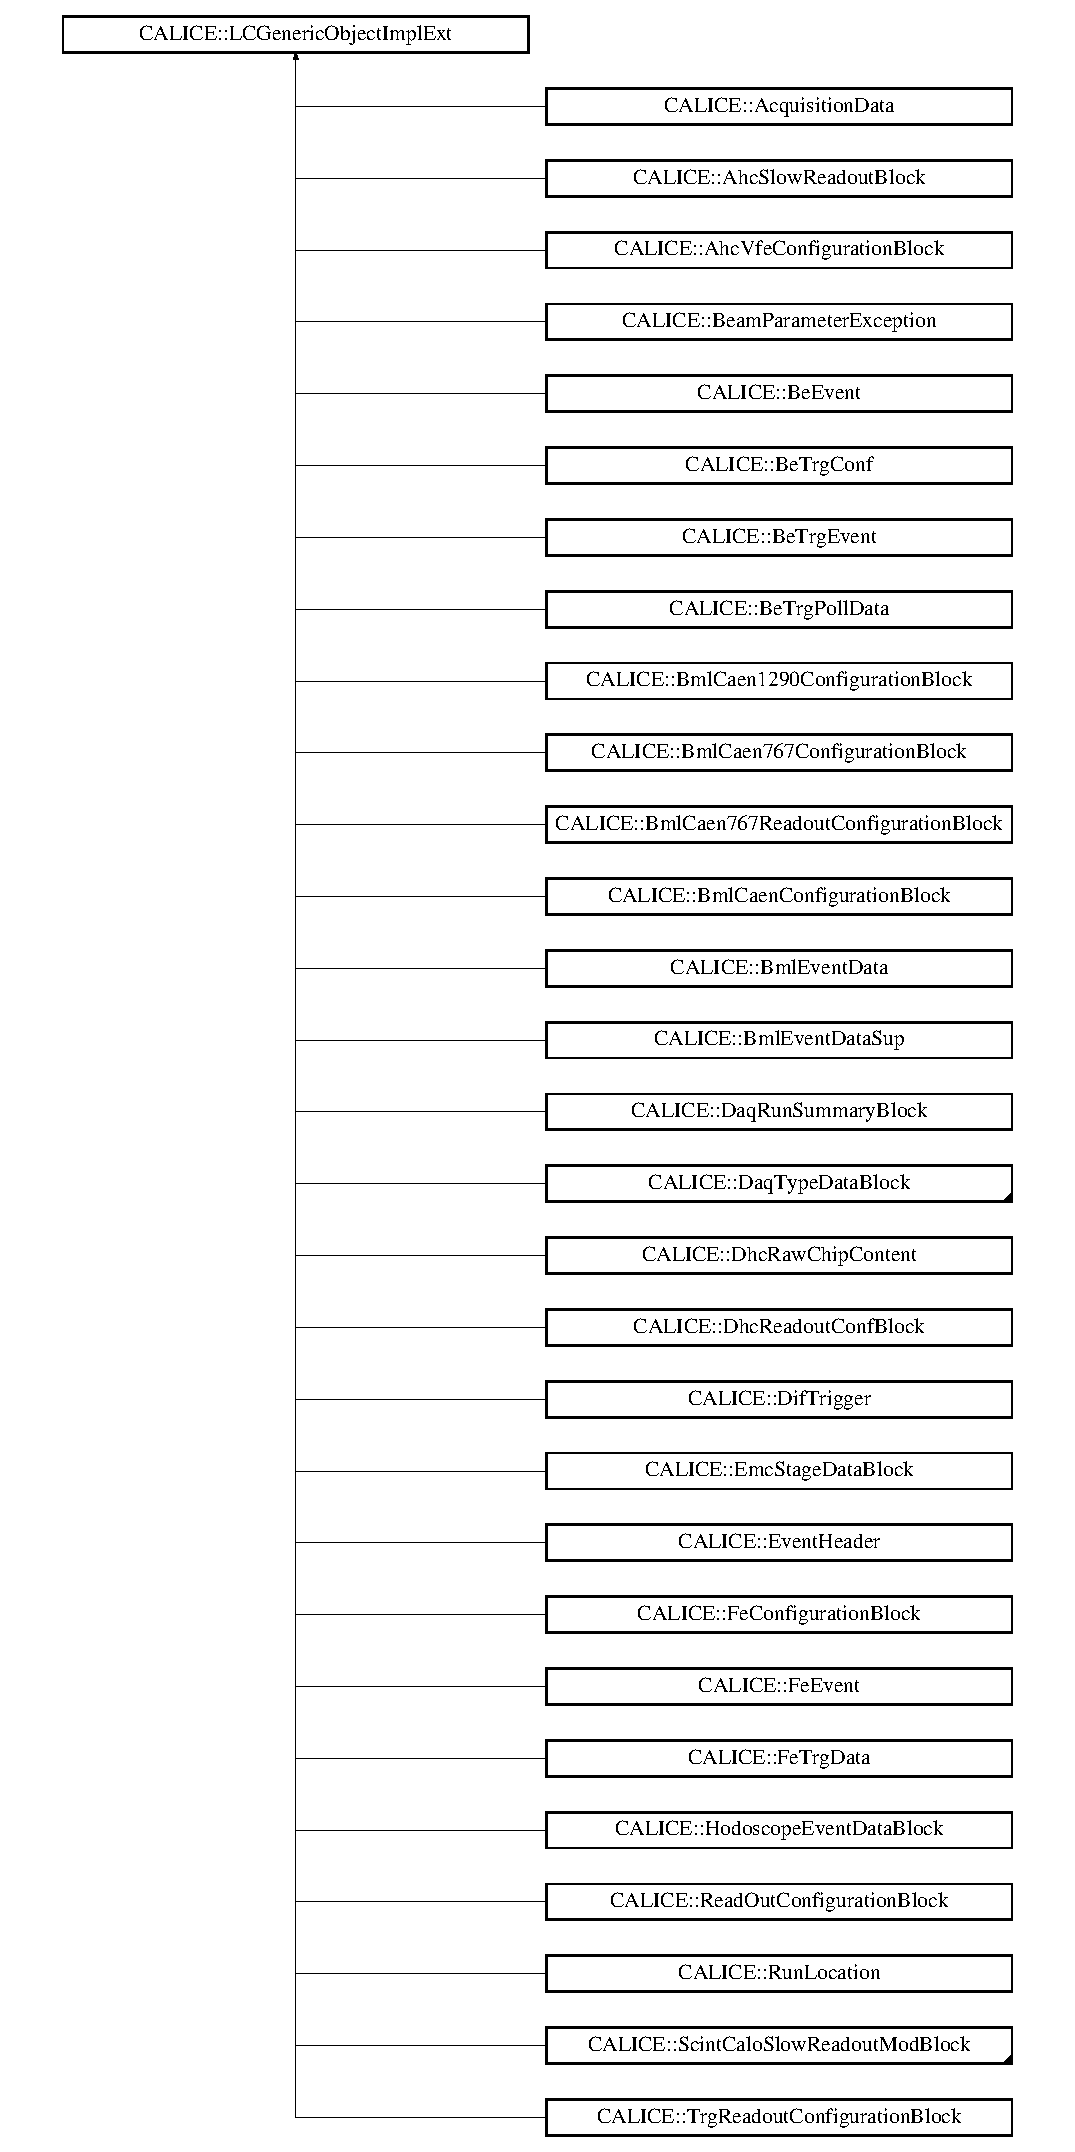
\includegraphics[height=12cm]{classCALICE_1_1LCGenericObjectImplExt}
\end{center}
\end{figure}
\subsection*{Public Member Functions}
\begin{DoxyCompactItemize}
\item 
{\bf LCGenericObjectImplExt} ()\label{classCALICE_1_1LCGenericObjectImplExt_aa3a6bb969c7cc736d88587960b663cba}

\begin{DoxyCompactList}\small\item\em Default c'tor. \item\end{DoxyCompactList}\item 
{\bfseries LCGenericObjectImplExt} (LCObject $\ast$obj)\label{classCALICE_1_1LCGenericObjectImplExt_a5e58ebbd98f49efeee560fd6bda8aae4}

\item 
LCGenericObjectImpl $\ast$ {\bf obj} ()
\begin{DoxyCompactList}\small\item\em The LCGenericObjectImpl . \item\end{DoxyCompactList}\item 
virtual {\bf $\sim$LCGenericObjectImplExt} ()\label{classCALICE_1_1LCGenericObjectImplExt_a6326844158718441a0e984402e9c2f8b}

\begin{DoxyCompactList}\small\item\em Clean up if we created a new LCGenericObjectImpl. \item\end{DoxyCompactList}\item 
virtual int {\bf id} ()\label{classCALICE_1_1LCGenericObjectImplExt_a13e336bf7a902820651dadb79271cd37}

\begin{DoxyCompactList}\small\item\em Return the id of the underlying LCGenericObjectImpl. \item\end{DoxyCompactList}\item 
int {\bfseries getNInt} () const \label{classCALICE_1_1LCGenericObjectImplExt_aee1c6e2485d45b6dcba643210f840224}

\item 
int {\bfseries getNFloat} () const \label{classCALICE_1_1LCGenericObjectImplExt_a09d41f70b6a4894b0f79806c32ead2b3}

\item 
int {\bfseries getNDouble} () const \label{classCALICE_1_1LCGenericObjectImplExt_aa8503a0fc8e66c4e0e374e32bb594231}

\item 
int {\bfseries getIntVal} (int index) const \label{classCALICE_1_1LCGenericObjectImplExt_a57a61745bb48cd3917ddf1ba37f8a3e0}

\item 
float {\bfseries getFloatVal} (int index) const \label{classCALICE_1_1LCGenericObjectImplExt_adda599738de7681f6c0d1b2aa3b09f79}

\item 
double {\bfseries getDoubleVal} (int index) const \label{classCALICE_1_1LCGenericObjectImplExt_ae10468f12c1a49ce00fceeb3f6664cbe}

\item 
bool {\bfseries isFixedSize} () const \label{classCALICE_1_1LCGenericObjectImplExt_ae546a36a343a9376e818e0b2d9a96e4d}

\end{DoxyCompactItemize}
\subsection*{Protected Attributes}
\begin{DoxyCompactItemize}
\item 
LCGenericObjectImpl $\ast$ {\bfseries \_\-obj}\label{classCALICE_1_1LCGenericObjectImplExt_a29179cf5508768d2cdbc9e2e6997bfdf}

\item 
bool {\bfseries \_\-createdObject}\label{classCALICE_1_1LCGenericObjectImplExt_a65c76ade794ece6642ce4a6fc0ed1a8f}

\end{DoxyCompactItemize}


\subsection{Detailed Description}
Extends functionality of the LCGenericObjectImpl Class It simply adds a new constructor to the LCGenericObject Class such that we can construct an interface class around without being restricted by the LCFixedObject It uses an instance of LCGenericObjectImpl that holds the data, thus there is no overhead when the data is read from a database or file for copying it to some local structure (Decorator pattern). \par
 This is still an abstract class: subclasses have to implement LCGenericObj ect::getTypeName() and LCGenericObject::getDataDescription(). It is basically a copy of the lcio::UTIL::LCFixedObject class I don't know whether this is the best solution, maybe it is better to use later on a real extension of the LCGenericObjectImpl \begin{DoxyAuthor}{Author}
Roman Poeschl, LAL Orsay 
\end{DoxyAuthor}
\begin{DoxyDate}{Date}
Feb. 2006 
\end{DoxyDate}


Definition at line 30 of file LCGenericObjectImplExt.hh.

\subsection{Member Function Documentation}
\index{CALICE::LCGenericObjectImplExt@{CALICE::LCGenericObjectImplExt}!obj@{obj}}
\index{obj@{obj}!CALICE::LCGenericObjectImplExt@{CALICE::LCGenericObjectImplExt}}
\subsubsection[{obj}]{\setlength{\rightskip}{0pt plus 5cm}LCGenericObjectImpl$\ast$ CALICE::LCGenericObjectImplExt::obj ()\hspace{0.3cm}{\ttfamily  [inline]}}\label{classCALICE_1_1LCGenericObjectImplExt_a7a6258e61fee4d6c67481e9e58a6062d}


The LCGenericObjectImpl . Sublcasses use this to access their data. 

Definition at line 74 of file LCGenericObjectImplExt.hh.

Referenced by CALICE::AcquisitionData::AcquisitionData(), CALICE::BmlEventData::addTDCChannels(), CALICE::AhcVfeConfigurationBlock::AhcVfeConfigurationBlock(), CALICE::BeTrgConf::BeTrgConf(), CALICE::BeTrgPollData::BeTrgPollData(), CALICE::FeConfigurationBlock::clearCalibEnable(), CALICE::FeConfigurationBlock::clearHoldInvert(), CALICE::DhcRawChipContent::DhcRawChipContent(), CALICE::DhcReadoutConfBlock::DhcReadoutConfBlock(), CALICE::FeConfigurationBlock::FeConfigurationBlock(), CALICE::DhcReadoutConfBlock::fillMethod(), CALICE::DhcReadoutConfBlock::fillSlotToWordsAssociationMask(), CALICE::DaqTypeDataBlock::finalize(), CALICE::AcquisitionData::getAcquisitionNumberInConfiguration(), CALICE::AcquisitionData::getAcquisitionNumberInRun(), CALICE::AcquisitionData::getActAcquisitionTimeMus(), CALICE::AcquisitionData::getActAcquisitionTimeSec(), CALICE::AcquisitionData::getActEventNumberInAcquisition(), CALICE::BeTrgPollData::getEndTime(), CALICE::EventHeader::getEventNumberInAcquisition(), CALICE::EventHeader::getEventNumberInConfiguration(), CALICE::EventHeader::getEventNumberInRun(), CALICE::AcquisitionData::getMaxAcquisitionTimeMus(), CALICE::AcquisitionData::getMaxAcquisitionTimeSec(), CALICE::AcquisitionData::getMaxEventNumberInAcquisition(), CALICE::BeTrgPollData::getMaximumTimeMus(), CALICE::BeTrgPollData::getMaximumTimeSec(), CALICE::BeTrgPollData::getNumberOfPolls(), CALICE::AhcVfeConfigurationBlock::getShiftRegisterData(), CALICE::BeTrgPollData::getStartTime(), CALICE::ScintCaloSlowReadoutModBlock::getTimeStamp(), CALICE::AhcVfeConfigurationBlock::getVerificationData(), CALICE::BeTrgPollData::isTimeout(), CALICE::DaqTypeDataBlock::RestoreMaps(), CALICE::BmlSlowRunDataBlock::setAbsorberPosition(), CALICE::AcquisitionData::setAcquisitionState(), CALICE::FeConfigurationBlock::setAdcControlBits(), CALICE::FeConfigurationBlock::setAdcDelay(), CALICE::FeConfigurationBlock::setAdcEnd(), CALICE::FeConfigurationBlock::setAdcStart(), CALICE::FeTrgData::setAllFifoWords(), CALICE::BeTrgEvent::setAllFifoWords(), CALICE::BeTrgConf::setAndEnable(), CALICE::BmlEventData::setBaseAddress(), CALICE::BeamParameterException::setBeamEnergy(), CALICE::ReadOutConfigurationBlock::setBecPeriod(), CALICE::ReadOutConfigurationBlock::setBePeriod(), CALICE::ReadOutConfigurationBlock::setBeSoftTrigger(), CALICE::TrgReadoutConfigurationBlock::setBeTrgPollNumber(), CALICE::TrgReadoutConfigurationBlock::setBeTrgPollTime(), CALICE::TrgReadoutConfigurationBlock::setBeTrgSoftSpill(), CALICE::TrgReadoutConfigurationBlock::setBeTrgSoftTrg(), CALICE::TrgReadoutConfigurationBlock::setBeTrgSpillNumber(), CALICE::TrgReadoutConfigurationBlock::setBeTrgSpillTime(), CALICE::TrgReadoutConfigurationBlock::setBeTrgSquirt(), CALICE::TrgReadoutConfigurationBlock::setBeTrgVlink(), CALICE::DhcReadoutConfBlock::setBeWaitInterval(), CALICE::FeConfigurationBlock::setBoardComponentNumber(), CALICE::AhcVfeConfigurationBlock::setBoardComponentNumber(), CALICE::FeTrgData::setBoardID(), CALICE::FeEvent::setBoardID(), CALICE::FeConfigurationBlock::setBoardID(), CALICE::BmlEventData::setBoardID(), CALICE::BeTrgPollData::setBoardID(), CALICE::BeTrgEvent::setBoardID(), CALICE::BeTrgConf::setBoardID(), CALICE::BeEvent::setBoardID(), CALICE::AhcVfeConfigurationBlock::setBoardID(), CALICE::BmlCaen767ReadoutConfigurationBlock::setBools(), CALICE::BmlEventDataSup::setBufferOverflow(), CALICE::BmlEventDataSup::setBunchID(), CALICE::BeTrgConf::setBurstCounter(), CALICE::BeTrgConf::setBurstTimeout(), CALICE::BeTrgConf::setBusyTimeout(), CALICE::BeEvent::setBxCounter(), CALICE::FeConfigurationBlock::setCalibEnable(), CALICE::FeConfigurationBlock::setCalibStart(), CALICE::FeConfigurationBlock::setCalibWidth(), CALICE::EmcStageDataBlock::setCheckSum(), CALICE::TrgReadoutConfigurationBlock::setClearBeTrg(), CALICE::ScintCaloSlowReadoutModBlock::setCmbHeight(), CALICE::ScintCaloSlowReadoutModBlock::setCmbWidth(), CALICE::BeTrgConf::setConfiguration(), CALICE::ReadOutConfigurationBlock::setConfMode(), CALICE::BeTrgEvent::setControl(), CALICE::ReadOutConfigurationBlock::setCrateID(), CALICE::FeConfigurationBlock::setCrateID(), CALICE::AhcVfeConfigurationBlock::setCrateID(), CALICE::DhcRawChipContent::setCrateNumber(), CALICE::BmlCaen767ReadoutConfigurationBlock::setCrateNumber(), CALICE::FeConfigurationBlock::setDacData(), CALICE::ScintCaloSlowReadoutModBlock::setDblArrays(), CALICE::BmlSlowRunDataBlock::setDblArrays(), CALICE::DhcRawChipContent::setDhcTimeStamp(), CALICE::AcquisitionData::setDifInfoPresent(), CALICE::AcquisitionData::setDifTriggerCounter(), CALICE::DhcRawChipContent::setElecChannel(), CALICE::FeConfigurationBlock::setEmcVfeInfo(), CALICE::TrgReadoutConfigurationBlock::setEnable(), CALICE::BeTrgPollData::setEndTime(), CALICE::BmlEventData::setEventDataCounter(), CALICE::BmlEventDataSup::setEventFifoCont(), CALICE::BmlEventDataSup::setEventIDTrailer(), CALICE::BmlEventData::setEventNumber(), CALICE::EventHeader::setEventNumberInAcquisition(), CALICE::EventHeader::setEventNumberInConfiguration(), CALICE::AcquisitionData::setEventNumberInfo(), CALICE::EventHeader::setEventNumberInRun(), CALICE::BeTrgConf::setExtBeamMode(), CALICE::ReadOutConfigurationBlock::setFeBrcSoftTrigger(), CALICE::ReadOutConfigurationBlock::setFePeriod(), CALICE::ReadOutConfigurationBlock::setFeSlotEnable(), CALICE::ReadOutConfigurationBlock::setFeSoftTrigger(), CALICE::BeTrgConf::setFifoIdleDepth(), CALICE::FeTrgData::setFifoWord(), CALICE::BeTrgEvent::setFifoWord(), CALICE::BeTrgEvent::setFinalFifoStatus(), CALICE::FeConfigurationBlock::setFrameSyncDelay(), CALICE::BeTrgConf::setGeneralEnable(), CALICE::BmlEventData::setGeoAddress(), CALICE::EmcStageDataBlock::setHeader(), CALICE::FeTrgData::setHeaderWord(), CALICE::DhcRawChipContent::setHitsHi(), CALICE::DhcRawChipContent::setHitsLo(), CALICE::FeConfigurationBlock::setHoldInvert(), CALICE::FeConfigurationBlock::setHoldStart(), CALICE::BeTrgEvent::setInitialFifoStatus(), CALICE::BeTrgEvent::setInputCatch(), CALICE::BeTrgConf::setInputEnableMask(), CALICE::BeTrgConf::setInputInvert(), CALICE::BeTrgEvent::setInputStatus(), CALICE::BeEvent::setL1aCounter(), CALICE::ScintCaloSlowReadoutModBlock::setLedSetting(), CALICE::DaqTypeDataBlock::setLengthIndexOfDblTypeNames(), CALICE::DaqTypeDataBlock::setLengthIndexOfFloatTypeNames(), CALICE::DaqTypeDataBlock::setLengthIndexOfIntTypeNames(), CALICE::DaqTypeDataBlock::setLengthIndexOfTimeStampNames(), CALICE::BeTrgPollData::setMaximumTime(), CALICE::DhcRawChipContent::setMiscInfo(), CALICE::BmlCaen767ReadoutConfigurationBlock::setMode(), CALICE::ScintCaloSlowReadoutModBlock::setModuleNumber(), CALICE::DaqRunSummaryBlock::setNumberOfAcquisitions(), CALICE::DaqRunSummaryBlock::setNumberOfConfigurations(), CALICE::DaqTypeDataBlock::setNumberOfDblTypes(), CALICE::AcquisitionData::setNumberofDifBufferWords(), CALICE::DaqRunSummaryBlock::setNumberOfEvents(), CALICE::DaqTypeDataBlock::setNumberOfFloatTypes(), CALICE::DaqTypeDataBlock::setNumberOfIntTypes(), CALICE::BeTrgPollData::setNumberOfPolls(), CALICE::BmlEventData::setNumberOfSignalChannels(), CALICE::DhcReadoutConfBlock::setNumberOfSlots(), CALICE::DaqRunSummaryBlock::setNumberOfSlowReadouts(), CALICE::DaqTypeDataBlock::setNumberOfTimeStamps(), CALICE::BmlEventData::setNumberOfWords(), CALICE::DhcReadoutConfBlock::setNumbers(), CALICE::ScintCaloSlowReadoutModBlock::setNumPos(), CALICE::BmlSlowRunDataBlock::setNumPos(), CALICE::BeTrgConf::setOscillationPeriod(), CALICE::BeTrgConf::setOscillatorEnable(), CALICE::DaqTypeDataBlock::setPointerToIndexOfDblTypeNames(), CALICE::DaqTypeDataBlock::setPointerToIndexOfFloatTypeNames(), CALICE::DaqTypeDataBlock::setPointerToIndexOfIntTypeNames(), CALICE::DaqTypeDataBlock::setPointerToIndexOfTimeStampNames(), CALICE::BeTrgEvent::setPreBusyCatch(), CALICE::BeTrgEvent::setPreBusyTriggerCounter(), CALICE::BeTrgConf::setQdrConfiguration(), CALICE::BeEvent::setQdrDataCounter(), CALICE::BeEvent::setQdrFrameCounter(), CALICE::TrgReadoutConfigurationBlock::setReadCounterPeriod(), CALICE::TrgReadoutConfigurationBlock::setReadPeriod(), CALICE::BmlCaen767ReadoutConfigurationBlock::setReadPeriod(), CALICE::FeTrgData::setRecordLabel(), CALICE::FeEvent::setRecordLabel(), CALICE::FeConfigurationBlock::setRecordLabel(), CALICE::BmlEventData::setRecordLabel(), CALICE::BeTrgPollData::setRecordLabel(), CALICE::BeTrgConf::setRecordLabel(), CALICE::BeEvent::setRecordLabel(), CALICE::AhcVfeConfigurationBlock::setRecordLabel(), CALICE::DaqRunSummaryBlock::setRunDuration(), CALICE::RunLocation::setRunLocationParameters(), CALICE::DaqRunSummaryBlock::setRunNumber(), CALICE::BeTrgConf::setSequencerControl(), CALICE::AhcVfeConfigurationBlock::setShiftRegisterData(), CALICE::BeTrgEvent::setSignalCatch(), CALICE::DaqTypeDataBlock::setSizeIndexOfDblType(), CALICE::DaqTypeDataBlock::setSizeIndexOfFloatType(), CALICE::DaqTypeDataBlock::setSizeIndexOfIntType(), CALICE::ReadOutConfigurationBlock::setSlotEnable(), CALICE::DhcReadoutConfBlock::setSlotEnable(), CALICE::DhcReadoutConfBlock::setSlotEnableMask(), CALICE::FeConfigurationBlock::setSlotID(), CALICE::AhcVfeConfigurationBlock::setSlotID(), CALICE::TrgReadoutConfigurationBlock::setSpillInvert(), CALICE::FeEvent::setSpyRegister(), CALICE::BeTrgPollData::setStartTime(), CALICE::BmlEventData::setStatus(), CALICE::BmlEventData::setStatusRegister(), CALICE::BeEvent::setStatusWord(), CALICE::BmlSlowRunDataBlock::setT4Position(), CALICE::BmlSlowRunDataBlock::setTargetPosition(), CALICE::BmlEventDataSup::setTDCErrors(), CALICE::BmlEventDataSup::setTDCType(), CALICE::BmlEventDataSup::setTDCWordCountTrailer(), CALICE::HodoscopeEventDataBlock::setTimeCounter(), CALICE::AcquisitionData::setTimeInformationMuSec(), CALICE::AcquisitionData::setTimeInformationSec(), CALICE::BeTrgPollData::setTimeout(), CALICE::ScintCaloSlowReadoutModBlock::setTimeStamp(), CALICE::BmlSlowRunDataBlock::setTimeStamp(), CALICE::BeEvent::setTotalFrameCounter(), CALICE::FeTrgData::setTrailerWord(), CALICE::FeTrgData::setTriggerCounter(), CALICE::FeEvent::setTriggerCounter(), CALICE::DifTrigger::setTriggerCounter(), CALICE::BeTrgEvent::setTriggerCounter(), CALICE::BmlEventDataSup::setTriggerLost(), CALICE::DaqTypeDataBlock::setTypeIndex(), CALICE::BmlEventDataSup::setTypeIndex(), CALICE::AhcVfeConfigurationBlock::setVerificationData(), CALICE::FeConfigurationBlock::setVfeInfo(), CALICE::FeConfigurationBlock::setVfeResetEnd(), CALICE::FeConfigurationBlock::setVfeResetStart(), CALICE::FeConfigurationBlock::setVfeSrinStart(), CALICE::ReadOutConfigurationBlock::setVmePeriod(), CALICE::EmcStageDataBlock::setXYStatus(), and CALICE::EmcStageDataBlock::setXYValues().

The documentation for this class was generated from the following file:\begin{DoxyCompactItemize}
\item 
LCGenericObjectImplExt.hh\end{DoxyCompactItemize}

\section{CALICE::LCHcalCalibrationObject Class Reference}
\label{classCALICE_1_1LCHcalCalibrationObject}\index{CALICE::LCHcalCalibrationObject@{CALICE::LCHcalCalibrationObject}}


Object to store information about arbitrary cell wise calibration of the HCAL in LC Objects.  


{\ttfamily \#include $<$LCHcalCalibrationObject.hh$>$}Inheritance diagram for CALICE::LCHcalCalibrationObject::\begin{figure}[H]
\begin{center}
\leavevmode
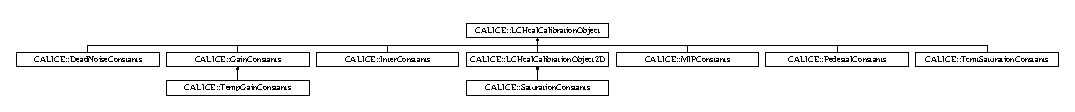
\includegraphics[height=1.05727cm]{classCALICE_1_1LCHcalCalibrationObject}
\end{center}
\end{figure}
\subsection*{Public Member Functions}
\begin{DoxyCompactItemize}
\item 
{\bf LCHcalCalibrationObject} ()\label{classCALICE_1_1LCHcalCalibrationObject_acb284f567fd1d0ad6ffe21b30f21cdaa}

\begin{DoxyCompactList}\small\item\em Default c'tor. \item\end{DoxyCompactList}\item 
{\bfseries LCHcalCalibrationObject} (LCObject $\ast$obj)\label{classCALICE_1_1LCHcalCalibrationObject_ac550a3a93ec37a835ebf980cd17f8d09}

\item 
LCGenericObjectImpl $\ast$ {\bf obj} ()
\begin{DoxyCompactList}\small\item\em The LCGenericObjectImpl . \item\end{DoxyCompactList}\item 
virtual {\bf $\sim$LCHcalCalibrationObject} ()\label{classCALICE_1_1LCHcalCalibrationObject_a2fdfef9c05ed0c8d69be6a6ac7e879d3}

\begin{DoxyCompactList}\small\item\em Clean up if we created a new LCGenericObjectImpl. \item\end{DoxyCompactList}\item 
virtual int {\bf id} ()\label{classCALICE_1_1LCHcalCalibrationObject_adfd871bb200ee6edc74e77ab99cd64cf}

\begin{DoxyCompactList}\small\item\em Return the id of the underlying LCGenericObjectImpl. \item\end{DoxyCompactList}\item 
int {\bfseries getNInt} () const \label{classCALICE_1_1LCHcalCalibrationObject_ab05f6cd6a589c3ce40d502b5789de97b}

\item 
int {\bfseries getNFloat} () const \label{classCALICE_1_1LCHcalCalibrationObject_ab0b0edbc06b75b1f79b7418f5a800bf5}

\item 
int {\bfseries getNDouble} () const \label{classCALICE_1_1LCHcalCalibrationObject_a8c3aebde0329827bed1847c06420ce36}

\item 
int {\bfseries getIntVal} (int index) const \label{classCALICE_1_1LCHcalCalibrationObject_a2dba956b310465eddc44d69ae8355277}

\item 
float {\bfseries getFloatVal} (int index) const \label{classCALICE_1_1LCHcalCalibrationObject_a37c7ae04e24cb2b923d765123d149b5b}

\item 
double {\bfseries getDoubleVal} (int index) const \label{classCALICE_1_1LCHcalCalibrationObject_a231f2119fb380bc4278227d6f1a7ca16}

\item 
bool {\bfseries isFixedSize} () const \label{classCALICE_1_1LCHcalCalibrationObject_a399a467018ef0e400cfaed6bc164f5e7}

\item 
float {\bfseries getConstant} ()\label{classCALICE_1_1LCHcalCalibrationObject_a9b41090c53867d347adecaad4dbb642c}

\item 
float {\bfseries getConstantError} ()\label{classCALICE_1_1LCHcalCalibrationObject_acc1cde393ee9e7bf8e7cf8c7de367366}

\item 
void {\bfseries setConstant} (float c)\label{classCALICE_1_1LCHcalCalibrationObject_a0b9f775ebdfe811203943fc88fa53747}

\item 
void {\bfseries setConstantError} (float ce)\label{classCALICE_1_1LCHcalCalibrationObject_aef6d9550f34c29a260ec80ecc3816550}

\item 
unsigned {\bf getCellKey} () const \label{classCALICE_1_1LCHcalCalibrationObject_ade3cd1a7657d6f0b759a814d884e74a7}

\begin{DoxyCompactList}\small\item\em get cell key of cell \item\end{DoxyCompactList}\item 
void {\bf setCellKey} (unsigned cellKey)\label{classCALICE_1_1LCHcalCalibrationObject_acefb80d278a76b9ee117de5f52274e4c}

\begin{DoxyCompactList}\small\item\em set cell key of cell \item\end{DoxyCompactList}\item 
unsigned {\bf getChip} () const \label{classCALICE_1_1LCHcalCalibrationObject_abf8d38197f79027123cc991c122472ec}

\begin{DoxyCompactList}\small\item\em get chip number of cell \item\end{DoxyCompactList}\item 
unsigned {\bf getChannel} () const \label{classCALICE_1_1LCHcalCalibrationObject_a6ec29045e1d20f2a0fb4169a4e017b12}

\begin{DoxyCompactList}\small\item\em get channel number of cell \item\end{DoxyCompactList}\item 
virtual float {\bf applyCalibration} (float inputValue) const 
\begin{DoxyCompactList}\small\item\em let the object apply the calibration stored in the object \item\end{DoxyCompactList}\item 
virtual float {\bf cancelCalibration} (float outputValue) const \label{classCALICE_1_1LCHcalCalibrationObject_a77e8c36b4989d3c378bce8c16ddbb2a9}

\begin{DoxyCompactList}\small\item\em cancel an applied calibration from energy value \item\end{DoxyCompactList}\item 
virtual float {\bf applyCalibrationError} (float inputValue, float inputError) const 
\begin{DoxyCompactList}\small\item\em let the object calculate the error after applying the calibration stored in the object \item\end{DoxyCompactList}\item 
virtual float {\bf cancelCalibrationError} (float outputValue, float outputError) const \label{classCALICE_1_1LCHcalCalibrationObject_abca1f2e349d568bc41f5576d7dc00f93}

\begin{DoxyCompactList}\small\item\em apply error due to canceling a calibration to current error \item\end{DoxyCompactList}\item 
virtual bool {\bf calibrationValid} () const 
\begin{DoxyCompactList}\small\item\em is the calibration stored in the object valid? \item\end{DoxyCompactList}\item 
virtual bool {\bf keepEvent} (float resultValue, float resultError) const 
\begin{DoxyCompactList}\small\item\em should the cell been kept in the cell selection after the calibration has been performed? \item\end{DoxyCompactList}\item 
virtual float {\bfseries getParam} (unsigned paramIndex) const \label{classCALICE_1_1LCHcalCalibrationObject_a9187cdf6f753d71c5f6753b90eb806c4}

\item 
virtual void {\bfseries setParam} (unsigned paramIndex)\label{classCALICE_1_1LCHcalCalibrationObject_a1fdd053f46ff8a7b21ff64232d4fcfcb}

\item 
virtual void {\bfseries setCellTemp} (float tempValue, float tempError)\label{classCALICE_1_1LCHcalCalibrationObject_a617cffebc3dd06251a671d77dc4df9b0}

\item 
virtual float {\bfseries getCellTemp} ()\label{classCALICE_1_1LCHcalCalibrationObject_a04d3b21769fcca6a86d2029c7f400f43}

\item 
virtual float {\bfseries getCellTempError} ()\label{classCALICE_1_1LCHcalCalibrationObject_a5178c01f738484bc55c49677a5476588}

\item 
const std::string {\bf getTypeName} () const \label{classCALICE_1_1LCHcalCalibrationObject_ace5c8bbdd0437badd08b6d09dfd75ae9}

\begin{DoxyCompactList}\small\item\em return type of the class \item\end{DoxyCompactList}\item 
const std::string {\bf getDataDescription} () const \label{classCALICE_1_1LCHcalCalibrationObject_a56c472a25d3146e4b152ce52116e44b9}

\begin{DoxyCompactList}\small\item\em return a brief description of the data member \item\end{DoxyCompactList}\end{DoxyCompactItemize}
\subsection*{Protected Attributes}
\begin{DoxyCompactItemize}
\item 
LCGenericObjectImpl $\ast$ {\bfseries \_\-obj}\label{classCALICE_1_1LCHcalCalibrationObject_a89c0628c58561dc3a036c1cce0d0d6ba}

\item 
bool {\bfseries \_\-createdObject}\label{classCALICE_1_1LCHcalCalibrationObject_a315d971845a1d05206d4502a141b5aba}

\end{DoxyCompactItemize}


\subsection{Detailed Description}
Object to store information about arbitrary cell wise calibration of the HCAL in LC Objects. \begin{DoxyAuthor}{Author}
S. Schmidt DESY 
\end{DoxyAuthor}
\begin{DoxyDate}{Date}
Jul 2006 
\end{DoxyDate}


Definition at line 20 of file LCHcalCalibrationObject.hh.

\subsection{Member Function Documentation}
\index{CALICE::LCHcalCalibrationObject@{CALICE::LCHcalCalibrationObject}!applyCalibration@{applyCalibration}}
\index{applyCalibration@{applyCalibration}!CALICE::LCHcalCalibrationObject@{CALICE::LCHcalCalibrationObject}}
\subsubsection[{applyCalibration}]{\setlength{\rightskip}{0pt plus 5cm}virtual float CALICE::LCHcalCalibrationObject::applyCalibration (float {\em inputValue}) const\hspace{0.3cm}{\ttfamily  [inline, virtual]}}\label{classCALICE_1_1LCHcalCalibrationObject_a763f1cf5b9c372fdde268d79b789adcc}


let the object apply the calibration stored in the object 
\begin{DoxyParams}{Parameters}
\item[{\em inputValue}]\char`\"{}energy\char`\"{} value of the cell before the calibration \end{DoxyParams}
\begin{DoxyReturn}{Returns}
\char`\"{}energy\char`\"{} value of the cell after the calibration 
\end{DoxyReturn}


Reimplemented in {\bf CALICE::DeadNoiseConstants} \doxyref{}{p.}{classCALICE_1_1DeadNoiseConstants_a117a93e472c84e57b805de35e12b6e29}, {\bf CALICE::GainConstants} \doxyref{}{p.}{classCALICE_1_1GainConstants_aeb089dc140f6e63d2f0a4746ecdd5cbb}, {\bf CALICE::InterConstants} \doxyref{}{p.}{classCALICE_1_1InterConstants_ac4e54f423b0048db8e79b745a53a5209}, {\bf CALICE::LCHcalCalibrationObject2D} \doxyref{}{p.}{classCALICE_1_1LCHcalCalibrationObject2D_ad805292313b3bb8fe8a3008a3f285b10}, {\bf CALICE::MIPConstants} \doxyref{}{p.}{classCALICE_1_1MIPConstants_a1ce8759ffdc72c9975ef2705c08fc4d7}, {\bf CALICE::PedestalConstants} \doxyref{}{p.}{classCALICE_1_1PedestalConstants_abbcc4190367b281e817a54467f7d7ed2}, {\bf CALICE::TcmtSaturationConstants} \doxyref{}{p.}{classCALICE_1_1TcmtSaturationConstants_a7a6e4f80607f938d3a739bf2527f3a56}, and {\bf CALICE::TempGainConstants} \doxyref{}{p.}{classCALICE_1_1TempGainConstants_ae2278e77d19368d5fb1ec5fb1eecef44}.

Definition at line 131 of file LCHcalCalibrationObject.hh.\index{CALICE::LCHcalCalibrationObject@{CALICE::LCHcalCalibrationObject}!applyCalibrationError@{applyCalibrationError}}
\index{applyCalibrationError@{applyCalibrationError}!CALICE::LCHcalCalibrationObject@{CALICE::LCHcalCalibrationObject}}
\subsubsection[{applyCalibrationError}]{\setlength{\rightskip}{0pt plus 5cm}virtual float CALICE::LCHcalCalibrationObject::applyCalibrationError (float {\em inputValue}, \/  float {\em inputError}) const\hspace{0.3cm}{\ttfamily  [inline, virtual]}}\label{classCALICE_1_1LCHcalCalibrationObject_a16d9de9567f68d7784a2daa4d2821341}


let the object calculate the error after applying the calibration stored in the object 
\begin{DoxyParams}{Parameters}
\item[{\em inputValue}]\char`\"{}energy\char`\"{} value of the cell stored before the calibration \item[{\em inputError}]error of the \char`\"{}energy\char`\"{} value of the cell before the calibration \end{DoxyParams}
\begin{DoxyReturn}{Returns}
error of the \char`\"{}energy\char`\"{} value of the cell after the calibration taking into account the error of the \char`\"{}energy\char`\"{} value of the cell before the calibration and the error of the calibration itself 
\end{DoxyReturn}


Reimplemented in {\bf CALICE::DeadNoiseConstants} \doxyref{}{p.}{classCALICE_1_1DeadNoiseConstants_a1c5558e71e236dabf1e54f54a87162f0}, {\bf CALICE::GainConstants} \doxyref{}{p.}{classCALICE_1_1GainConstants_a669886b01357faa0b2173384be3a60d3}, {\bf CALICE::InterConstants} \doxyref{}{p.}{classCALICE_1_1InterConstants_ad102c242709f9229f3936d04bb356be7}, {\bf CALICE::LCHcalCalibrationObject2D} \doxyref{}{p.}{classCALICE_1_1LCHcalCalibrationObject2D_a5a73278000f9d13e19969bc229fe18f3}, {\bf CALICE::MIPConstants} \doxyref{}{p.}{classCALICE_1_1MIPConstants_a7beb08be64e40e822288cf285b5601e0}, {\bf CALICE::PedestalConstants} \doxyref{}{p.}{classCALICE_1_1PedestalConstants_ac2c94c3d42b510de4c973ffb4a463469}, {\bf CALICE::TcmtSaturationConstants} \doxyref{}{p.}{classCALICE_1_1TcmtSaturationConstants_a256def068f131f98cb3a62669cc4dcaa}, and {\bf CALICE::TempGainConstants} \doxyref{}{p.}{classCALICE_1_1TempGainConstants_a4319810d19fd6bb61de44faec1f56226}.

Definition at line 148 of file LCHcalCalibrationObject.hh.\index{CALICE::LCHcalCalibrationObject@{CALICE::LCHcalCalibrationObject}!calibrationValid@{calibrationValid}}
\index{calibrationValid@{calibrationValid}!CALICE::LCHcalCalibrationObject@{CALICE::LCHcalCalibrationObject}}
\subsubsection[{calibrationValid}]{\setlength{\rightskip}{0pt plus 5cm}virtual bool CALICE::LCHcalCalibrationObject::calibrationValid () const\hspace{0.3cm}{\ttfamily  [inline, virtual]}}\label{classCALICE_1_1LCHcalCalibrationObject_abbb1fce81f41a89147b721d593bbc734}


is the calibration stored in the object valid? \begin{DoxyReturn}{Returns}
true if the calibration is valid, false if no valid calibration is available 
\end{DoxyReturn}


Reimplemented in {\bf CALICE::DeadNoiseConstants} \doxyref{}{p.}{classCALICE_1_1DeadNoiseConstants_ad7e3bc3298b47d8fa31a43c160a8a45b}, {\bf CALICE::GainConstants} \doxyref{}{p.}{classCALICE_1_1GainConstants_a37c5d66f2537eee42e259147856e86a7}, {\bf CALICE::InterConstants} \doxyref{}{p.}{classCALICE_1_1InterConstants_ab184f4d15b941b5ac67474b02eaab138}, {\bf CALICE::MIPConstants} \doxyref{}{p.}{classCALICE_1_1MIPConstants_aba936e2505ba100025495dded661ccb0}, {\bf CALICE::PedestalConstants} \doxyref{}{p.}{classCALICE_1_1PedestalConstants_a6cfd6a82fa83433d2abe95b830ae164d}, {\bf CALICE::SaturationConstants} \doxyref{}{p.}{classCALICE_1_1SaturationConstants_a7fdebcaa3ebf3b099aa11524e347ace3}, {\bf CALICE::TcmtSaturationConstants} \doxyref{}{p.}{classCALICE_1_1TcmtSaturationConstants_aa2b6117fdcb356a8af69f54a2944a0af}, and {\bf CALICE::TempGainConstants} \doxyref{}{p.}{classCALICE_1_1TempGainConstants_a132d04dd01b328d85857bda95baf000b}.

Definition at line 161 of file LCHcalCalibrationObject.hh.\index{CALICE::LCHcalCalibrationObject@{CALICE::LCHcalCalibrationObject}!keepEvent@{keepEvent}}
\index{keepEvent@{keepEvent}!CALICE::LCHcalCalibrationObject@{CALICE::LCHcalCalibrationObject}}
\subsubsection[{keepEvent}]{\setlength{\rightskip}{0pt plus 5cm}virtual bool CALICE::LCHcalCalibrationObject::keepEvent (float {\em resultValue}, \/  float {\em resultError}) const\hspace{0.3cm}{\ttfamily  [inline, virtual]}}\label{classCALICE_1_1LCHcalCalibrationObject_a59f14a6b83e77717751ae4e7213e8d09}


should the cell been kept in the cell selection after the calibration has been performed? 
\begin{DoxyParams}{Parameters}
\item[{\em resultValue}]\char`\"{}energy\char`\"{} value of the cell after the calibration \item[{\em resultError}]error on the \char`\"{}energy\char`\"{} value of the cell after the calibration \end{DoxyParams}


Reimplemented in {\bf CALICE::DeadNoiseConstants} \doxyref{}{p.}{classCALICE_1_1DeadNoiseConstants_af4318e256ff1466682855553d5ba453e}, {\bf CALICE::GainConstants} \doxyref{}{p.}{classCALICE_1_1GainConstants_a18c349f2f60b6f2d5d387fe386c63ebc}, {\bf CALICE::InterConstants} \doxyref{}{p.}{classCALICE_1_1InterConstants_a919e037d3e03029486c2a3c9713e772a}, {\bf CALICE::MIPConstants} \doxyref{}{p.}{classCALICE_1_1MIPConstants_a11232a43c70405ef3f8c4cc88641de6a}, {\bf CALICE::PedestalConstants} \doxyref{}{p.}{classCALICE_1_1PedestalConstants_a5296ca6178fa8cebd290bcae2f39a86f}, {\bf CALICE::SaturationConstants} \doxyref{}{p.}{classCALICE_1_1SaturationConstants_a4df07d49bfccab7e7586bffddee8583c}, and {\bf CALICE::TcmtSaturationConstants} \doxyref{}{p.}{classCALICE_1_1TcmtSaturationConstants_adb8d6310076d321706941a73904e4f02}.

Definition at line 169 of file LCHcalCalibrationObject.hh.\index{CALICE::LCHcalCalibrationObject@{CALICE::LCHcalCalibrationObject}!obj@{obj}}
\index{obj@{obj}!CALICE::LCHcalCalibrationObject@{CALICE::LCHcalCalibrationObject}}
\subsubsection[{obj}]{\setlength{\rightskip}{0pt plus 5cm}LCGenericObjectImpl$\ast$ CALICE::LCHcalCalibrationObject::obj ()\hspace{0.3cm}{\ttfamily  [inline]}}\label{classCALICE_1_1LCHcalCalibrationObject_a3d930fab870a493259f89039a2716bf9}


The LCGenericObjectImpl . Sublcasses use this to access their data. 

Definition at line 64 of file LCHcalCalibrationObject.hh.

Referenced by CALICE::DeadNoiseConstants::DeadNoiseConstants(), CALICE::GainConstants::GainConstants(), CALICE::TempGainConstants::setGainTemp(), CALICE::TempGainConstants::setTslope(), and CALICE::TempGainConstants::TempGainConstants().

The documentation for this class was generated from the following file:\begin{DoxyCompactItemize}
\item 
LCHcalCalibrationObject.hh\end{DoxyCompactItemize}

\section{CALICE::LCHcalCalibrationObject2D Class Reference}
\label{classCALICE_1_1LCHcalCalibrationObject2D}\index{CALICE::LCHcalCalibrationObject2D@{CALICE::LCHcalCalibrationObject2D}}


The results of the calibrations done by \doxyref{LCHcalCalibrationObject2D}{p.}{classCALICE_1_1LCHcalCalibrationObject2D} can depend on two sets of input values (like saturation correction).  


{\ttfamily \#include $<$LCHcalCalibrationObject2D.hh$>$}Inheritance diagram for CALICE::LCHcalCalibrationObject2D::\begin{figure}[H]
\begin{center}
\leavevmode
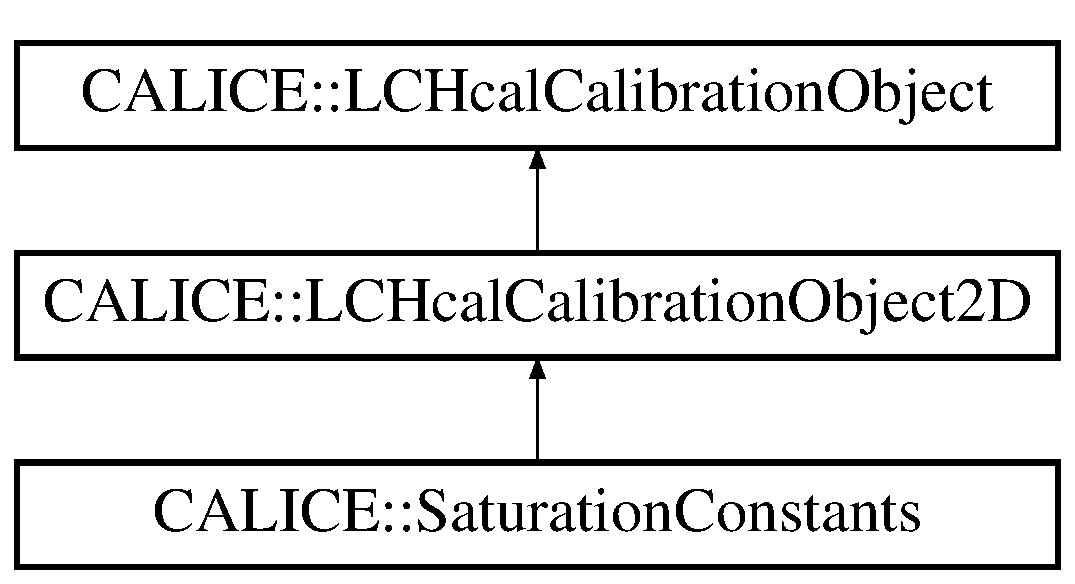
\includegraphics[height=3cm]{classCALICE_1_1LCHcalCalibrationObject2D}
\end{center}
\end{figure}
\subsection*{Public Member Functions}
\begin{DoxyCompactItemize}
\item 
{\bfseries LCHcalCalibrationObject2D} (LCObject $\ast$obj)\label{classCALICE_1_1LCHcalCalibrationObject2D_a9d0b2e8a75de8cd23d1425d4221141f2}

\item 
virtual float {\bfseries applyCalibration} (float inputValue, float inputParameter) const \label{classCALICE_1_1LCHcalCalibrationObject2D_a9e63a4d12f105fcea5e0faf73b4a34c9}

\item 
virtual float {\bfseries applyCalibrationError} (float inputValue, float inputError, float inputParameter, float inputParameterError) const \label{classCALICE_1_1LCHcalCalibrationObject2D_a48eb6be23a1512823a40c5597101eec1}

\item 
virtual float {\bf applyCalibration} (float inputValue) const 
\begin{DoxyCompactList}\small\item\em let the object apply the calibration stored in the object \item\end{DoxyCompactList}\item 
virtual float {\bf applyCalibrationError} (float inputValue, float inputError) const 
\begin{DoxyCompactList}\small\item\em let the object calculate the error after applying the calibration stored in the object \item\end{DoxyCompactList}\end{DoxyCompactItemize}


\subsection{Detailed Description}
The results of the calibrations done by \doxyref{LCHcalCalibrationObject2D}{p.}{classCALICE_1_1LCHcalCalibrationObject2D} can depend on two sets of input values (like saturation correction). \begin{DoxyAuthor}{Author}
S. Schmidt, DESY 
\end{DoxyAuthor}
\begin{DoxyDate}{Date}
September 2006 
\end{DoxyDate}


Definition at line 21 of file LCHcalCalibrationObject2D.hh.

\subsection{Member Function Documentation}
\index{CALICE::LCHcalCalibrationObject2D@{CALICE::LCHcalCalibrationObject2D}!applyCalibration@{applyCalibration}}
\index{applyCalibration@{applyCalibration}!CALICE::LCHcalCalibrationObject2D@{CALICE::LCHcalCalibrationObject2D}}
\subsubsection[{applyCalibration}]{\setlength{\rightskip}{0pt plus 5cm}virtual float CALICE::LCHcalCalibrationObject2D::applyCalibration (float {\em inputValue}) const\hspace{0.3cm}{\ttfamily  [inline, virtual]}}\label{classCALICE_1_1LCHcalCalibrationObject2D_ad805292313b3bb8fe8a3008a3f285b10}


let the object apply the calibration stored in the object 
\begin{DoxyParams}{Parameters}
\item[{\em inputValue}]\char`\"{}energy\char`\"{} value of the cell before the calibration \end{DoxyParams}
\begin{DoxyReturn}{Returns}
\char`\"{}energy\char`\"{} value of the cell after the calibration 
\end{DoxyReturn}


Reimplemented from {\bf CALICE::LCHcalCalibrationObject} \doxyref{}{p.}{classCALICE_1_1LCHcalCalibrationObject_a763f1cf5b9c372fdde268d79b789adcc}.

Definition at line 37 of file LCHcalCalibrationObject2D.hh.\index{CALICE::LCHcalCalibrationObject2D@{CALICE::LCHcalCalibrationObject2D}!applyCalibrationError@{applyCalibrationError}}
\index{applyCalibrationError@{applyCalibrationError}!CALICE::LCHcalCalibrationObject2D@{CALICE::LCHcalCalibrationObject2D}}
\subsubsection[{applyCalibrationError}]{\setlength{\rightskip}{0pt plus 5cm}virtual float CALICE::LCHcalCalibrationObject2D::applyCalibrationError (float {\em inputValue}, \/  float {\em inputError}) const\hspace{0.3cm}{\ttfamily  [inline, virtual]}}\label{classCALICE_1_1LCHcalCalibrationObject2D_a5a73278000f9d13e19969bc229fe18f3}


let the object calculate the error after applying the calibration stored in the object 
\begin{DoxyParams}{Parameters}
\item[{\em inputValue}]\char`\"{}energy\char`\"{} value of the cell stored before the calibration \item[{\em inputError}]error of the \char`\"{}energy\char`\"{} value of the cell before the calibration \end{DoxyParams}
\begin{DoxyReturn}{Returns}
error of the \char`\"{}energy\char`\"{} value of the cell after the calibration taking into account the error of the \char`\"{}energy\char`\"{} value of the cell before the calibration and the error of the calibration itself 
\end{DoxyReturn}


Reimplemented from {\bf CALICE::LCHcalCalibrationObject} \doxyref{}{p.}{classCALICE_1_1LCHcalCalibrationObject_a16d9de9567f68d7784a2daa4d2821341}.

Definition at line 41 of file LCHcalCalibrationObject2D.hh.

The documentation for this class was generated from the following file:\begin{DoxyCompactItemize}
\item 
LCHcalCalibrationObject2D.hh\end{DoxyCompactItemize}

\section{CALICE::LinearFitCompound Class Reference}
\label{classCALICE_1_1LinearFitCompound}\index{CALICE::LinearFitCompound@{CALICE::LinearFitCompound}}


Class to store the constant of a linear fit within the lcio framework.  


{\ttfamily \#include $<$LinearFitCompound.hh$>$}\subsection*{Public Member Functions}
\begin{DoxyCompactItemize}
\item 
{\bfseries LinearFitCompound} (lcio::LCObject $\ast$obj)\label{classCALICE_1_1LinearFitCompound_aa041bdcd07656d399c777cb69d3df568}

\item 
{\bfseries LinearFitCompound} (const {\bf LinearFitConstant} $\ast$lfc, const {\bf LinearFitSlope} $\ast$lfs)\label{classCALICE_1_1LinearFitCompound_a8f5ac3c81a865ecc10f36e22bdb8e94f}

\item 
{\bfseries LinearFitCompound} (int ID, double constant, double constant\_\-error, double constant\_\-reference\_\-point, double constant\_\-reference\_\-point\_\-error, double slope, double slope\_\-error)\label{classCALICE_1_1LinearFitCompound_aa9bea1b2c7c021daa57dc3542288c1ac}

\item 
double {\bf eval} (double x)
\begin{DoxyCompactList}\small\item\em Evaluates the linear fit at the given point. \item\end{DoxyCompactList}\item 
double {\bfseries evalErr} (double x, double x\_\-error)\label{classCALICE_1_1LinearFitCompound_a78b246859cb94fc056e66b65544f8d65}

\item 
int {\bf getID} () const \label{classCALICE_1_1LinearFitCompound_a9cd94ca37460ca86c74fd4e659f280cc}

\begin{DoxyCompactList}\small\item\em Get the identifier. \item\end{DoxyCompactList}\item 
double {\bf getConstant} () const \label{classCALICE_1_1LinearFitCompound_ac1ca6ec7539fe980fbd67af7769930d3}

\begin{DoxyCompactList}\small\item\em Get the constant/y-\/intercept of the fit. \item\end{DoxyCompactList}\item 
double {\bf getConstantError} () const \label{classCALICE_1_1LinearFitCompound_a1c512b13cee1df98953e18eff78047ac}

\begin{DoxyCompactList}\small\item\em Get the error of the constant. \item\end{DoxyCompactList}\item 
double {\bf getSlope} () const \label{classCALICE_1_1LinearFitCompound_adb11c7794278351a448df3bff3a0bd07}

\begin{DoxyCompactList}\small\item\em Get slope of the linear fit. \item\end{DoxyCompactList}\item 
double {\bf getSlopeError} () const \label{classCALICE_1_1LinearFitCompound_a19e287bdba39f38751496a5b06f28569}

\begin{DoxyCompactList}\small\item\em Get error of the slope. \item\end{DoxyCompactList}\item 
double {\bf getConstantReferencePoint} () const \label{classCALICE_1_1LinearFitCompound_a72a91d14525eedaa7f2f436f6c7fe51e}

\begin{DoxyCompactList}\small\item\em Get the reference point of the constant. \item\end{DoxyCompactList}\item 
double {\bf getConstantReferencePointError} () const \label{classCALICE_1_1LinearFitCompound_a77547513303b8e9df5329c5dd67571ac}

\begin{DoxyCompactList}\small\item\em Get the error of the reference point of the constant. \item\end{DoxyCompactList}\item 
void {\bf setID} (const int ID)\label{classCALICE_1_1LinearFitCompound_af7dcd74ed57f41b64c7ba082c8070246}

\begin{DoxyCompactList}\small\item\em Sets an identifier. \item\end{DoxyCompactList}\item 
void {\bf setConstant} (const double constant)\label{classCALICE_1_1LinearFitCompound_a144ad1196e206d632f000939097d80aa}

\begin{DoxyCompactList}\small\item\em Sets the constant. \item\end{DoxyCompactList}\item 
void {\bf setConstantError} (double constantError)\label{classCALICE_1_1LinearFitCompound_aa990f347871e140731ae76b27277efc7}

\begin{DoxyCompactList}\small\item\em Sets the error of the constant. \item\end{DoxyCompactList}\item 
void {\bf setSlope} (const double slope)\label{classCALICE_1_1LinearFitCompound_afed1ff8b17afcaee84727a41ace77349}

\begin{DoxyCompactList}\small\item\em Sets the slope. \item\end{DoxyCompactList}\item 
void {\bf setSlopeError} (const double slope\_\-error)\label{classCALICE_1_1LinearFitCompound_af8761b938e369b0daaa1ec258db93a7e}

\begin{DoxyCompactList}\small\item\em Sets the error of the slope. \item\end{DoxyCompactList}\item 
void {\bf setConstantReferencePoint} (const double constantReferencePoint)\label{classCALICE_1_1LinearFitCompound_a9f694715ade079c8e0e8af5496707e37}

\begin{DoxyCompactList}\small\item\em Sets the reference point of the constant. \item\end{DoxyCompactList}\item 
void {\bf setConstantReferencePointError} (double constantReferencePointError)\label{classCALICE_1_1LinearFitCompound_a0e2c5570c83bbb2e3f3a0e9124258d4f}

\begin{DoxyCompactList}\small\item\em Sets the error of the reference point of the constant. \item\end{DoxyCompactList}\item 
const std::string {\bf getTypeName} () const 
\begin{DoxyCompactList}\small\item\em Get the type name. \item\end{DoxyCompactList}\item 
const std::string {\bf getDataDescription} () const 
\begin{DoxyCompactList}\small\item\em Get the data description. \item\end{DoxyCompactList}\end{DoxyCompactItemize}


\subsection{Detailed Description}
Class to store the constant of a linear fit within the lcio framework. \begin{DoxyAuthor}{Author}
LNTAI 
\end{DoxyAuthor}
\begin{DoxyVersion}{Version}
1.0 
\end{DoxyVersion}
\begin{DoxyDate}{Date}
27 October 2009 
\end{DoxyDate}


Definition at line 37 of file LinearFitCompound.hh.

\subsection{Member Function Documentation}
\index{CALICE::LinearFitCompound@{CALICE::LinearFitCompound}!eval@{eval}}
\index{eval@{eval}!CALICE::LinearFitCompound@{CALICE::LinearFitCompound}}
\subsubsection[{eval}]{\setlength{\rightskip}{0pt plus 5cm}double CALICE::LinearFitCompound::eval (double {\em x})\hspace{0.3cm}{\ttfamily  [inline]}}\label{classCALICE_1_1LinearFitCompound_a6a90eaa22d28b9223e5c67800cb41192}


Evaluates the linear fit at the given point. 
\begin{DoxyParams}{Parameters}
\item[{\em x}]-\/ the point at which the fit is evaluated \end{DoxyParams}


Definition at line 97 of file LinearFitCompound.hh.

References getConstant(), getConstantReferencePoint(), and getSlope().\index{CALICE::LinearFitCompound@{CALICE::LinearFitCompound}!getDataDescription@{getDataDescription}}
\index{getDataDescription@{getDataDescription}!CALICE::LinearFitCompound@{CALICE::LinearFitCompound}}
\subsubsection[{getDataDescription}]{\setlength{\rightskip}{0pt plus 5cm}const std::string CALICE::LinearFitCompound::getDataDescription () const\hspace{0.3cm}{\ttfamily  [inline]}}\label{classCALICE_1_1LinearFitCompound_ae44e7e243c8e2a030324852b4c1f1dd2}


Get the data description. The data description gives the meaning of the data fields. 

Definition at line 247 of file LinearFitCompound.hh.\index{CALICE::LinearFitCompound@{CALICE::LinearFitCompound}!getTypeName@{getTypeName}}
\index{getTypeName@{getTypeName}!CALICE::LinearFitCompound@{CALICE::LinearFitCompound}}
\subsubsection[{getTypeName}]{\setlength{\rightskip}{0pt plus 5cm}const std::string CALICE::LinearFitCompound::getTypeName () const\hspace{0.3cm}{\ttfamily  [inline]}}\label{classCALICE_1_1LinearFitCompound_a1479fcbd624f1452277f65bda2e3f65b}


Get the type name. The type name is used to determine which class interprets the LCGenericObject which holds the pure data. 

Definition at line 238 of file LinearFitCompound.hh.

The documentation for this class was generated from the following file:\begin{DoxyCompactItemize}
\item 
LinearFitCompound.hh\end{DoxyCompactItemize}

\section{CALICE::LinearFitConstant Class Reference}
\label{classCALICE_1_1LinearFitConstant}\index{CALICE::LinearFitConstant@{CALICE::LinearFitConstant}}


Class to store the constant of a linear fit within the lcio framework.  


{\ttfamily \#include $<$LinearFitConstant.hh$>$}\subsection*{Public Member Functions}
\begin{DoxyCompactItemize}
\item 
{\bfseries LinearFitConstant} (lcio::LCObject $\ast$obj)\label{classCALICE_1_1LinearFitConstant_aad304d55b35c64a6ccc10f6678bea491}

\item 
{\bfseries LinearFitConstant} (int ID, double constant, double constant\_\-error, double constant\_\-reference\_\-point, double constant\_\-reference\_\-point\_\-error)\label{classCALICE_1_1LinearFitConstant_ab237e9f47438621313de684f516b5eea}

\item 
double {\bf eval} (double x)
\begin{DoxyCompactList}\small\item\em In the case of a given corresponding slope this functions evaluates the linear fit at the given point. \item\end{DoxyCompactList}\item 
int {\bf getID} () const \label{classCALICE_1_1LinearFitConstant_ad6dac20732c9065577e04b1057d4cba5}

\begin{DoxyCompactList}\small\item\em Get the identifier. \item\end{DoxyCompactList}\item 
double {\bf getConstant} () const \label{classCALICE_1_1LinearFitConstant_a4d3578f48272ce09e288dde99c7081bf}

\begin{DoxyCompactList}\small\item\em Get the constant/y-\/intercept of the fit. \item\end{DoxyCompactList}\item 
double {\bf getConstantError} () const \label{classCALICE_1_1LinearFitConstant_a91e9290960a2d85f39938b46cfe3f92b}

\begin{DoxyCompactList}\small\item\em Get the error of the constant. \item\end{DoxyCompactList}\item 
double {\bf getConstantReferencePoint} () const \label{classCALICE_1_1LinearFitConstant_aa8748414106f0a3dc6bf7b5f406e2b88}

\begin{DoxyCompactList}\small\item\em Get the reference point of the constant. \item\end{DoxyCompactList}\item 
double {\bf getConstantReferencePointError} () const \label{classCALICE_1_1LinearFitConstant_a7c977c3a9db317ed19f895e047fc02a2}

\begin{DoxyCompactList}\small\item\em Get the error of the reference point of the constant. \item\end{DoxyCompactList}\item 
void {\bf setID} (const int ID)\label{classCALICE_1_1LinearFitConstant_a2c386d168d63ee9cf76f2381401daaa0}

\begin{DoxyCompactList}\small\item\em Sets an identifier. \item\end{DoxyCompactList}\item 
void {\bf setConstant} (const double constant)\label{classCALICE_1_1LinearFitConstant_a3b016378df601216e55545308334e1d8}

\begin{DoxyCompactList}\small\item\em Sets the constant. \item\end{DoxyCompactList}\item 
void {\bf setConstantError} (double constantError)\label{classCALICE_1_1LinearFitConstant_aa096484667f26f82589cc0745310564d}

\begin{DoxyCompactList}\small\item\em Sets the error of the constant. \item\end{DoxyCompactList}\item 
void {\bf setConstantReferencePoint} (const double constantReferencePoint)\label{classCALICE_1_1LinearFitConstant_aad5420fa51f86f5fc8a038b97794289b}

\begin{DoxyCompactList}\small\item\em Sets the reference point of the constant. \item\end{DoxyCompactList}\item 
void {\bf setConstantReferencePointError} (double constantReferencePointError)\label{classCALICE_1_1LinearFitConstant_a7ed2758698bd0da83348812817c4395a}

\begin{DoxyCompactList}\small\item\em Sets the error of the reference point of the constant. \item\end{DoxyCompactList}\item 
void {\bf setSlope} (double lfs)
\begin{DoxyCompactList}\small\item\em Sets a corresponding slope. \item\end{DoxyCompactList}\item 
const std::string {\bf getTypeName} () const 
\begin{DoxyCompactList}\small\item\em Get the type name. \item\end{DoxyCompactList}\item 
const std::string {\bf getDataDescription} () const 
\begin{DoxyCompactList}\small\item\em Get the data description. \item\end{DoxyCompactList}\end{DoxyCompactItemize}
\subsection*{Private Attributes}
\begin{DoxyCompactItemize}
\item 
bool {\bfseries \_\-linearFitSlopeAvailable}\label{classCALICE_1_1LinearFitConstant_a9e340a4dfbc49f5664a348ea97bf7c5a}

\item 
double {\bfseries \_\-linearFitSlope}\label{classCALICE_1_1LinearFitConstant_aa335a19743f509655fe5bf8a00563a82}

\end{DoxyCompactItemize}


\subsection{Detailed Description}
Class to store the constant of a linear fit within the lcio framework. \begin{DoxyAuthor}{Author}
Sebastian Schmitt ({\tt sebastian.richter@desy.de}) 
\end{DoxyAuthor}
\begin{DoxyVersion}{Version}
1.0 
\end{DoxyVersion}
\begin{DoxyDate}{Date}
16 February 2009 
\end{DoxyDate}


Definition at line 32 of file LinearFitConstant.hh.

\subsection{Member Function Documentation}
\index{CALICE::LinearFitConstant@{CALICE::LinearFitConstant}!eval@{eval}}
\index{eval@{eval}!CALICE::LinearFitConstant@{CALICE::LinearFitConstant}}
\subsubsection[{eval}]{\setlength{\rightskip}{0pt plus 5cm}double CALICE::LinearFitConstant::eval (double {\em x})\hspace{0.3cm}{\ttfamily  [inline]}}\label{classCALICE_1_1LinearFitConstant_a24c9412dcfa0de7b06a4083610afb68f}


In the case of a given corresponding slope this functions evaluates the linear fit at the given point. 
\begin{DoxyParams}{Parameters}
\item[{\em x}]-\/ the point at which the fit is evaluated \end{DoxyParams}


Definition at line 72 of file LinearFitConstant.hh.

References getConstant(), and getConstantReferencePoint().\index{CALICE::LinearFitConstant@{CALICE::LinearFitConstant}!getDataDescription@{getDataDescription}}
\index{getDataDescription@{getDataDescription}!CALICE::LinearFitConstant@{CALICE::LinearFitConstant}}
\subsubsection[{getDataDescription}]{\setlength{\rightskip}{0pt plus 5cm}const std::string CALICE::LinearFitConstant::getDataDescription () const\hspace{0.3cm}{\ttfamily  [inline]}}\label{classCALICE_1_1LinearFitConstant_ae2b2c8efbda731c2968ecc5ca4da5772}


Get the data description. The data description gives the meaning of the data fields. 

Definition at line 209 of file LinearFitConstant.hh.\index{CALICE::LinearFitConstant@{CALICE::LinearFitConstant}!getTypeName@{getTypeName}}
\index{getTypeName@{getTypeName}!CALICE::LinearFitConstant@{CALICE::LinearFitConstant}}
\subsubsection[{getTypeName}]{\setlength{\rightskip}{0pt plus 5cm}const std::string CALICE::LinearFitConstant::getTypeName () const\hspace{0.3cm}{\ttfamily  [inline]}}\label{classCALICE_1_1LinearFitConstant_a1929abfb9351d5273fed48ab3609c1c8}


Get the type name. The type name is used to determine which class interprets the LCGenericObject which holds the pure data. 

Definition at line 200 of file LinearFitConstant.hh.\index{CALICE::LinearFitConstant@{CALICE::LinearFitConstant}!setSlope@{setSlope}}
\index{setSlope@{setSlope}!CALICE::LinearFitConstant@{CALICE::LinearFitConstant}}
\subsubsection[{setSlope}]{\setlength{\rightskip}{0pt plus 5cm}void CALICE::LinearFitConstant::setSlope (double {\em lfs})\hspace{0.3cm}{\ttfamily  [inline]}}\label{classCALICE_1_1LinearFitConstant_ad2b647ad849fd025df318e9722d3673d}


Sets a corresponding slope. It is \_\-bad\_\- design to have this function here. But I really want to avoid another wrapping function combining the constant and the slope. So, sorry! 

Definition at line 187 of file LinearFitConstant.hh.

The documentation for this class was generated from the following file:\begin{DoxyCompactItemize}
\item 
LinearFitConstant.hh\end{DoxyCompactItemize}

\section{CALICE::LinearFitResult Class Reference}
\label{classCALICE_1_1LinearFitResult}\index{CALICE::LinearFitResult@{CALICE::LinearFitResult}}


Class to store the result of a linear fit within the lcio framework.  


{\ttfamily \#include $<$LinearFitResultLCIO.hh$>$}\subsection*{Public Member Functions}
\begin{DoxyCompactItemize}
\item 
{\bfseries LinearFitResult} (lcio::LCObject $\ast$obj)\label{classCALICE_1_1LinearFitResult_a787a52733606fc1285b8658bad6dcdb7}

\item 
{\bfseries LinearFitResult} (int ID, double offset, double slope, double chi2, double eMA, double eMB, double eMC, double eMD, int ndf)\label{classCALICE_1_1LinearFitResult_a2ab09e1e28ceec3d4d38954450d91d14}

\item 
double {\bf eval} (const double x) const 
\begin{DoxyCompactList}\small\item\em Evaluates the fit. \item\end{DoxyCompactList}\item 
int {\bf getID} () const \label{classCALICE_1_1LinearFitResult_a1d6731c9a204443691b3cd9d345e4e25}

\begin{DoxyCompactList}\small\item\em Get the identifier. \item\end{DoxyCompactList}\item 
int {\bf getNDF} () const \label{classCALICE_1_1LinearFitResult_ad0d3cd32c74891ff558a5685b7b6c52b}

\begin{DoxyCompactList}\small\item\em Get the number of degress of freedom of the fit. \item\end{DoxyCompactList}\item 
double {\bf getOffset} () const 
\begin{DoxyCompactList}\small\item\em Get the offset/y-\/intercept of the fit. \item\end{DoxyCompactList}\item 
double {\bf getSlope} () const \label{classCALICE_1_1LinearFitResult_a3337a69b522aebd8ee22712230461be9}

\begin{DoxyCompactList}\small\item\em Get the slope of the fit. \item\end{DoxyCompactList}\item 
double {\bf getChi2} () const \label{classCALICE_1_1LinearFitResult_ad8f1e8471fea87e81ea8804d2a6425b9}

\begin{DoxyCompactList}\small\item\em Get the Chi2 of the fit. \item\end{DoxyCompactList}\item 
void {\bf getErrorMatrix} (double errorMatrix[2][2]) const 
\begin{DoxyCompactList}\small\item\em Get the error matrix of the fit. \item\end{DoxyCompactList}\item 
double {\bf getOffsetError} () const \label{classCALICE_1_1LinearFitResult_a3672f98b7f1065e167e3be9fc33e9a5b}

\begin{DoxyCompactList}\small\item\em Get the error of the offset. \item\end{DoxyCompactList}\item 
double {\bf getSlopeError} () const \label{classCALICE_1_1LinearFitResult_a1f6bb8ac0767fd30c51f6f6737a16d0e}

\begin{DoxyCompactList}\small\item\em Get the error of the slope. \item\end{DoxyCompactList}\item 
void {\bf setID} (const int ID)\label{classCALICE_1_1LinearFitResult_a60030ae12b6d53fe2e8ee89431ac9e61}

\begin{DoxyCompactList}\small\item\em Sets an identifier. \item\end{DoxyCompactList}\item 
void {\bf setNDF} (const int NDF)\label{classCALICE_1_1LinearFitResult_a12be9eabc9b90be240a585a54047ed4a}

\begin{DoxyCompactList}\small\item\em Sets the number of degress of freedom. \item\end{DoxyCompactList}\item 
void {\bf setOffset} (const double offset)\label{classCALICE_1_1LinearFitResult_ac7d3cb3852250e6b792b1bf3de462afe}

\begin{DoxyCompactList}\small\item\em Sets the offset. \item\end{DoxyCompactList}\item 
void {\bf setSlope} (const double slope)\label{classCALICE_1_1LinearFitResult_ade777ec026d47bd9d5dd45119cbf2e7b}

\begin{DoxyCompactList}\small\item\em Sets the slope. \item\end{DoxyCompactList}\item 
void {\bf setChi2} (const double chi2)\label{classCALICE_1_1LinearFitResult_acd102f0b28cca3588b332e95029dec73}

\begin{DoxyCompactList}\small\item\em Sets the chi2. \item\end{DoxyCompactList}\item 
void {\bf setErrorMatrix} (const double array[2][2])\label{classCALICE_1_1LinearFitResult_a07626f2f4cb7e780421ccce480071410}

\begin{DoxyCompactList}\small\item\em Sets the full error matrix. \item\end{DoxyCompactList}\item 
void {\bf setOffsetError} (double offsetError)\label{classCALICE_1_1LinearFitResult_a2700899a5606c26906e6dea452fcb96c}

\begin{DoxyCompactList}\small\item\em Sets the error of the offset. \item\end{DoxyCompactList}\item 
void {\bf setSlopeError} (double slopeError)\label{classCALICE_1_1LinearFitResult_affe82cd5cd4c19a143545006f35e5859}

\begin{DoxyCompactList}\small\item\em Sets the error of the slope. \item\end{DoxyCompactList}\item 
const std::string {\bf getTypeName} () const 
\begin{DoxyCompactList}\small\item\em Get the type name. \item\end{DoxyCompactList}\item 
const std::string {\bf getDataDescription} () const 
\begin{DoxyCompactList}\small\item\em Get the data description. \item\end{DoxyCompactList}\end{DoxyCompactItemize}


\subsection{Detailed Description}
Class to store the result of a linear fit within the lcio framework. This class can be used for example to store the result of a linear fit, e.g. TF1 root fit.

Errors are stored in the error matrix.

\begin{DoxyAuthor}{Author}
Sebastian Richter ({\tt sebastian.richter@desy.de}) 
\end{DoxyAuthor}
\begin{DoxyVersion}{Version}
1.0 
\end{DoxyVersion}
\begin{DoxyDate}{Date}
9 January 2009 
\end{DoxyDate}


Definition at line 42 of file LinearFitResultLCIO.hh.

\subsection{Member Function Documentation}
\index{CALICE::LinearFitResult@{CALICE::LinearFitResult}!eval@{eval}}
\index{eval@{eval}!CALICE::LinearFitResult@{CALICE::LinearFitResult}}
\subsubsection[{eval}]{\setlength{\rightskip}{0pt plus 5cm}double CALICE::LinearFitResult::eval (const double {\em x}) const\hspace{0.3cm}{\ttfamily  [inline]}}\label{classCALICE_1_1LinearFitResult_ad7c907bb78608e51f09223d6c9e2290f}


Evaluates the fit. 
\begin{DoxyParams}{Parameters}
\item[{\em x}]-\/ point where the fit is evaluated: \doxyref{getOffset()}{p.}{classCALICE_1_1LinearFitResult_a7b982ced1ea8f7560298e70d86fcfa4e} + x $\ast$ \doxyref{getSlope()}{p.}{classCALICE_1_1LinearFitResult_a3337a69b522aebd8ee22712230461be9} \end{DoxyParams}


Definition at line 76 of file LinearFitResultLCIO.hh.

References getOffset(), and getSlope().\index{CALICE::LinearFitResult@{CALICE::LinearFitResult}!getDataDescription@{getDataDescription}}
\index{getDataDescription@{getDataDescription}!CALICE::LinearFitResult@{CALICE::LinearFitResult}}
\subsubsection[{getDataDescription}]{\setlength{\rightskip}{0pt plus 5cm}const std::string CALICE::LinearFitResult::getDataDescription () const\hspace{0.3cm}{\ttfamily  [inline]}}\label{classCALICE_1_1LinearFitResult_a50a70fb6361ffbb6a8ba34377c6a779c}


Get the data description. The data description gives the meaning of the data fields. 

Definition at line 244 of file LinearFitResultLCIO.hh.\index{CALICE::LinearFitResult@{CALICE::LinearFitResult}!getErrorMatrix@{getErrorMatrix}}
\index{getErrorMatrix@{getErrorMatrix}!CALICE::LinearFitResult@{CALICE::LinearFitResult}}
\subsubsection[{getErrorMatrix}]{\setlength{\rightskip}{0pt plus 5cm}void CALICE::LinearFitResult::getErrorMatrix (double {\em errorMatrix}[2][2]) const\hspace{0.3cm}{\ttfamily  [inline]}}\label{classCALICE_1_1LinearFitResult_a0a732a0fbe0bbda0b824166a172dac6b}


Get the error matrix of the fit. The first parameter is the offset, the second one is the slope. 

Definition at line 130 of file LinearFitResultLCIO.hh.

Referenced by getOffsetError(), and getSlopeError().\index{CALICE::LinearFitResult@{CALICE::LinearFitResult}!getOffset@{getOffset}}
\index{getOffset@{getOffset}!CALICE::LinearFitResult@{CALICE::LinearFitResult}}
\subsubsection[{getOffset}]{\setlength{\rightskip}{0pt plus 5cm}double CALICE::LinearFitResult::getOffset () const\hspace{0.3cm}{\ttfamily  [inline]}}\label{classCALICE_1_1LinearFitResult_a7b982ced1ea8f7560298e70d86fcfa4e}


Get the offset/y-\/intercept of the fit. The offset is equivalent to eval(0). 

Definition at line 103 of file LinearFitResultLCIO.hh.

Referenced by eval().\index{CALICE::LinearFitResult@{CALICE::LinearFitResult}!getTypeName@{getTypeName}}
\index{getTypeName@{getTypeName}!CALICE::LinearFitResult@{CALICE::LinearFitResult}}
\subsubsection[{getTypeName}]{\setlength{\rightskip}{0pt plus 5cm}const std::string CALICE::LinearFitResult::getTypeName () const\hspace{0.3cm}{\ttfamily  [inline]}}\label{classCALICE_1_1LinearFitResult_ab5d08f559ea52f1e9fe67053e6af787e}


Get the type name. The type name is used to determine which class interprets the LCGenericObject which holds the pure data. 

Definition at line 235 of file LinearFitResultLCIO.hh.

The documentation for this class was generated from the following file:\begin{DoxyCompactItemize}
\item 
LinearFitResultLCIO.hh\end{DoxyCompactItemize}

\section{CALICE::LinearFitSlope Class Reference}
\label{classCALICE_1_1LinearFitSlope}\index{CALICE::LinearFitSlope@{CALICE::LinearFitSlope}}


Class to store the slope of a linear fit within the lcio framework.  


{\ttfamily \#include $<$LinearFitSlope.hh$>$}\subsection*{Public Member Functions}
\begin{DoxyCompactItemize}
\item 
{\bfseries LinearFitSlope} (lcio::LCObject $\ast$obj)\label{classCALICE_1_1LinearFitSlope_a56c966d126341015453783e858b5afda}

\item 
{\bfseries LinearFitSlope} (int ID, double slope, double slope\_\-error)\label{classCALICE_1_1LinearFitSlope_a4d769bd2d4bc5bd2d7cc7136f04092da}

\item 
int {\bf getID} () const \label{classCALICE_1_1LinearFitSlope_af64381cf56c2cae77c77d4a476638197}

\begin{DoxyCompactList}\small\item\em Get the identifier. \item\end{DoxyCompactList}\item 
double {\bf getSlope} () const 
\begin{DoxyCompactList}\small\item\em Get the slope/y-\/intercept of the fit. \item\end{DoxyCompactList}\item 
double {\bf getSlopeError} () const \label{classCALICE_1_1LinearFitSlope_aab0ecd9b3ecff1110159c335e4efd3c2}

\begin{DoxyCompactList}\small\item\em Get the error of the slope. \item\end{DoxyCompactList}\item 
void {\bf setID} (const int ID)\label{classCALICE_1_1LinearFitSlope_ad6db15cec37ac81794b4ac73c8c4894d}

\begin{DoxyCompactList}\small\item\em Sets an identifier. \item\end{DoxyCompactList}\item 
void {\bf setSlope} (const double slope)\label{classCALICE_1_1LinearFitSlope_a0d35587b2fb909e93cc04391b6167e37}

\begin{DoxyCompactList}\small\item\em Sets the slope. \item\end{DoxyCompactList}\item 
void {\bf setSlopeError} (double slopeError)\label{classCALICE_1_1LinearFitSlope_a7ded89ec05a1418e1ee13a83b87d8b47}

\begin{DoxyCompactList}\small\item\em Sets the error of the slope. \item\end{DoxyCompactList}\item 
const std::string {\bf getTypeName} () const 
\begin{DoxyCompactList}\small\item\em Get the type name. \item\end{DoxyCompactList}\item 
const std::string {\bf getDataDescription} () const 
\begin{DoxyCompactList}\small\item\em Get the data description. \item\end{DoxyCompactList}\end{DoxyCompactItemize}


\subsection{Detailed Description}
Class to store the slope of a linear fit within the lcio framework. \begin{DoxyAuthor}{Author}
Sebastian Schmitt ({\tt sebastian.richter@desy.de}) 
\end{DoxyAuthor}
\begin{DoxyVersion}{Version}
1.0 
\end{DoxyVersion}
\begin{DoxyDate}{Date}
16 February 2009 
\end{DoxyDate}


Definition at line 27 of file LinearFitSlope.hh.

\subsection{Member Function Documentation}
\index{CALICE::LinearFitSlope@{CALICE::LinearFitSlope}!getDataDescription@{getDataDescription}}
\index{getDataDescription@{getDataDescription}!CALICE::LinearFitSlope@{CALICE::LinearFitSlope}}
\subsubsection[{getDataDescription}]{\setlength{\rightskip}{0pt plus 5cm}const std::string CALICE::LinearFitSlope::getDataDescription () const\hspace{0.3cm}{\ttfamily  [inline]}}\label{classCALICE_1_1LinearFitSlope_a46800ea9d0356523b21f8442f84b2780}


Get the data description. The data description gives the meaning of the data fields. 

Definition at line 112 of file LinearFitSlope.hh.\index{CALICE::LinearFitSlope@{CALICE::LinearFitSlope}!getSlope@{getSlope}}
\index{getSlope@{getSlope}!CALICE::LinearFitSlope@{CALICE::LinearFitSlope}}
\subsubsection[{getSlope}]{\setlength{\rightskip}{0pt plus 5cm}double CALICE::LinearFitSlope::getSlope () const\hspace{0.3cm}{\ttfamily  [inline]}}\label{classCALICE_1_1LinearFitSlope_a6647803adff8207d96d9c3990c4254f4}


Get the slope/y-\/intercept of the fit. The slope is equivalent to eval(0). 

Definition at line 60 of file LinearFitSlope.hh.\index{CALICE::LinearFitSlope@{CALICE::LinearFitSlope}!getTypeName@{getTypeName}}
\index{getTypeName@{getTypeName}!CALICE::LinearFitSlope@{CALICE::LinearFitSlope}}
\subsubsection[{getTypeName}]{\setlength{\rightskip}{0pt plus 5cm}const std::string CALICE::LinearFitSlope::getTypeName () const\hspace{0.3cm}{\ttfamily  [inline]}}\label{classCALICE_1_1LinearFitSlope_acead1fa7eff10fa3d589a79410c14f67}


Get the type name. The type name is used to determine which class interprets the LCGenericObject which holds the pure data. 

Definition at line 103 of file LinearFitSlope.hh.

The documentation for this class was generated from the following file:\begin{DoxyCompactItemize}
\item 
LinearFitSlope.hh\end{DoxyCompactItemize}

\section{LinearRegression Class Reference}
\label{classLinearRegression}\index{LinearRegression@{LinearRegression}}


Linear regression analysis of given value pairs.  


{\ttfamily \#include $<$LinearRegression.hh$>$}\subsection*{Public Member Functions}
\begin{DoxyCompactItemize}
\item 
void {\bf reset} ()\label{classLinearRegression_af538779ee8e289d026d799c3c7a426d1}

\begin{DoxyCompactList}\small\item\em initialise for a analysis of a new value set. \item\end{DoxyCompactList}\item 
{\bf LinearRegression} \& {\bf add} (Double\_\-t x, Double\_\-t y, Double\_\-t y\_\-error)\label{classLinearRegression_a0a3ab51f5d3931f905037a3c1f5bb98c}

\begin{DoxyCompactList}\small\item\em Add a value pair where the second values has the given uncertainty. \item\end{DoxyCompactList}\item 
{\bf LinearRegression} \& {\bf add} (Double\_\-t x, Double\_\-t y)\label{classLinearRegression_a3e12eed9356ba00d6d030bc1b57e3836}

\begin{DoxyCompactList}\small\item\em Add a value pair (if the uncertainty of the y-\/values is not known or are all the same). \item\end{DoxyCompactList}\item 
{\bf LinearRegression} \& {\bf add} (const {\bf LinearRegression} \&a)\label{classLinearRegression_ad1ac36ccba440cd93ef159bc0262f369}

\begin{DoxyCompactList}\small\item\em Add the values of another regression object to this object. \item\end{DoxyCompactList}\item 
{\bf LinearRegression} \& {\bf subtract} (Double\_\-t x, Double\_\-t y, Double\_\-t y\_\-error)
\begin{DoxyCompactList}\small\item\em Remove a value pair from the object. \item\end{DoxyCompactList}\item 
{\bf LinearRegression} \& {\bf subtract} (Double\_\-t x, Double\_\-t y)\label{classLinearRegression_ab3e8334bd774f51c91c2fe95da552615}

\begin{DoxyCompactList}\small\item\em Remove a value pair from the object (if the value pair has been added without specifying an uncertainty) May be called after an object has been added without specifying the uncertainty to remove it. \item\end{DoxyCompactList}\item 
{\bf LinearRegression} \& {\bf Subtract} (const {\bf LinearRegression} \&a)\label{classLinearRegression_a1951a036633b7322a6aac6d7bbad62d3}

\begin{DoxyCompactList}\small\item\em Remove all value pairs added to another regression object from this regression object. \item\end{DoxyCompactList}\item 
{\bf LinearRegression} \& {\bf calc} ()\label{classLinearRegression_a8ca4e29af63ac292213acbb4c48acc66}

\begin{DoxyCompactList}\small\item\em Calculate the ascent and the offset. \item\end{DoxyCompactList}\item 
{\bf LinearRegression} \& {\bf calcWithErrors} ()\label{classLinearRegression_ad1ce1e257093d3f89ebe8dc2e304c35c}

\begin{DoxyCompactList}\small\item\em Calculate the ascent and the offset and their errors. \item\end{DoxyCompactList}\item 
Double\_\-t {\bf offset} ()
\begin{DoxyCompactList}\small\item\em Return the calculated offset. \item\end{DoxyCompactList}\item 
Double\_\-t {\bf ascent} ()
\begin{DoxyCompactList}\small\item\em Return the calculated ascent. \item\end{DoxyCompactList}\item 
Double\_\-t {\bf eval} (Double\_\-t x)
\begin{DoxyCompactList}\small\item\em Calculate the best guess of y for the given value of x. \item\end{DoxyCompactList}\item 
Double\_\-t {\bf evalError} (Double\_\-t x, Double\_\-t x\_\-ref)
\begin{DoxyCompactList}\small\item\em Calculate the uncertainty of a certain y for the given value of x. \item\end{DoxyCompactList}\item 
Double\_\-t {\bf evalError} (Double\_\-t x)
\begin{DoxyCompactList}\small\item\em Calculate the uncertainty of a certain y for the given value of x. \item\end{DoxyCompactList}\item 
Double\_\-t {\bf sumOfWeights} ()\label{classLinearRegression_a1b6ad46cb0ee53f2c565687ad37d7ef5}

\begin{DoxyCompactList}\small\item\em Sum of the inverse uncertainties of the given y-\/values. \item\end{DoxyCompactList}\end{DoxyCompactItemize}
\subsection*{Data Fields}
\begin{DoxyCompactItemize}
\item 
Double\_\-t {\bfseries \_\-ascent}\label{classLinearRegression_a9fe4c687adadd779b0f7c406eca60fec}

\item 
Double\_\-t {\bfseries \_\-offset}\label{classLinearRegression_a9fe46d99a76240920d2ee973e80577a8}

\item 
Double\_\-t {\bfseries \_\-ascentError}\label{classLinearRegression_ad55f646d063c80c4cef00f4f17d6a7ca}

\item 
Double\_\-t {\bfseries \_\-offsetError}\label{classLinearRegression_ad75550f2ee31877c7675cc582fee5781}

\item 
Double\_\-t {\bfseries \_\-sumOfWeights}\label{classLinearRegression_ab21e8031c06270dec932d76fa391415e}

\item 
Double\_\-t {\bfseries \_\-sumX}\label{classLinearRegression_af0defb9c14f585b3efec8bb9e7974a9d}

\item 
Double\_\-t {\bfseries \_\-sumY}\label{classLinearRegression_a157369a9e88d3157cbe579ee074706ee}

\item 
Double\_\-t {\bfseries \_\-sumXX}\label{classLinearRegression_a44f6410b5baf2e0960a712a2102bde7b}

\item 
Double\_\-t {\bfseries \_\-sumXY}\label{classLinearRegression_aecf91d1e065dbfc79d0301a52707539c}

\item 
Double\_\-t {\bfseries \_\-sumYY}\label{classLinearRegression_a12c2c878e3e33551c6ce6bbc1c5ab0d7}

\end{DoxyCompactItemize}


\subsection{Detailed Description}
Linear regression analysis of given value pairs. 

Definition at line 17 of file LinearRegression.hh.

\subsection{Member Function Documentation}
\index{LinearRegression@{LinearRegression}!ascent@{ascent}}
\index{ascent@{ascent}!LinearRegression@{LinearRegression}}
\subsubsection[{ascent}]{\setlength{\rightskip}{0pt plus 5cm}Double\_\-t LinearRegression::ascent ()\hspace{0.3cm}{\ttfamily  [inline]}}\label{classLinearRegression_a3cc2c3590db57409dbb6d49db7b2d093}


Return the calculated ascent. The result is undefined before \doxyref{calc}{p.}{classLinearRegression_a8ca4e29af63ac292213acbb4c48acc66} or \doxyref{calcWithErrors}{p.}{classLinearRegression_ad1ce1e257093d3f89ebe8dc2e304c35c} was called. 

Definition at line 142 of file LinearRegression.hh.\index{LinearRegression@{LinearRegression}!eval@{eval}}
\index{eval@{eval}!LinearRegression@{LinearRegression}}
\subsubsection[{eval}]{\setlength{\rightskip}{0pt plus 5cm}Double\_\-t LinearRegression::eval (Double\_\-t {\em x})\hspace{0.3cm}{\ttfamily  [inline]}}\label{classLinearRegression_ad719ed942f31fe4aed9e5b8c92479c03}


Calculate the best guess of y for the given value of x. Calcualte \doxyref{offset()}{p.}{classLinearRegression_ad6441285eb22865d9308cee33cbbda17}+ascent()$\ast$x; The result is undefined before \doxyref{calc}{p.}{classLinearRegression_a8ca4e29af63ac292213acbb4c48acc66} or \doxyref{calcWithErrors}{p.}{classLinearRegression_ad1ce1e257093d3f89ebe8dc2e304c35c} was called. 

Definition at line 148 of file LinearRegression.hh.\index{LinearRegression@{LinearRegression}!evalError@{evalError}}
\index{evalError@{evalError}!LinearRegression@{LinearRegression}}
\subsubsection[{evalError}]{\setlength{\rightskip}{0pt plus 5cm}Double\_\-t LinearRegression::evalError (Double\_\-t {\em x})\hspace{0.3cm}{\ttfamily  [inline]}}\label{classLinearRegression_a16d080824a28976f242f2a35cb5bcb09}


Calculate the uncertainty of a certain y for the given value of x. The result is undefined before \doxyref{calc}{p.}{classLinearRegression_a8ca4e29af63ac292213acbb4c48acc66} or \doxyref{calcWithErrors}{p.}{classLinearRegression_ad1ce1e257093d3f89ebe8dc2e304c35c} was called. 

Definition at line 165 of file LinearRegression.hh.\index{LinearRegression@{LinearRegression}!evalError@{evalError}}
\index{evalError@{evalError}!LinearRegression@{LinearRegression}}
\subsubsection[{evalError}]{\setlength{\rightskip}{0pt plus 5cm}Double\_\-t LinearRegression::evalError (Double\_\-t {\em x}, \/  Double\_\-t {\em x\_\-ref})\hspace{0.3cm}{\ttfamily  [inline]}}\label{classLinearRegression_a6cca97556c3d8eae41f3961ee90ce951}


Calculate the uncertainty of a certain y for the given value of x. 
\begin{DoxyParams}{Parameters}
\item[{\em x}]the x value for which the uncertainty on y should be calculated \item[{\em x\_\-ref}]the x value at which the uncertainty is only given by the uncertainty of the \doxyref{offset()}{p.}{classLinearRegression_ad6441285eb22865d9308cee33cbbda17} should be the average x value of the input set. The result is undefined before \doxyref{calc}{p.}{classLinearRegression_a8ca4e29af63ac292213acbb4c48acc66} or \doxyref{calcWithErrors}{p.}{classLinearRegression_ad1ce1e257093d3f89ebe8dc2e304c35c} was called. \end{DoxyParams}


Definition at line 156 of file LinearRegression.hh.\index{LinearRegression@{LinearRegression}!offset@{offset}}
\index{offset@{offset}!LinearRegression@{LinearRegression}}
\subsubsection[{offset}]{\setlength{\rightskip}{0pt plus 5cm}Double\_\-t LinearRegression::offset ()\hspace{0.3cm}{\ttfamily  [inline]}}\label{classLinearRegression_ad6441285eb22865d9308cee33cbbda17}


Return the calculated offset. The result is undefined before \doxyref{calc}{p.}{classLinearRegression_a8ca4e29af63ac292213acbb4c48acc66} or \doxyref{calcWithErrors}{p.}{classLinearRegression_ad1ce1e257093d3f89ebe8dc2e304c35c} was called. 

Definition at line 137 of file LinearRegression.hh.\index{LinearRegression@{LinearRegression}!subtract@{subtract}}
\index{subtract@{subtract}!LinearRegression@{LinearRegression}}
\subsubsection[{subtract}]{\setlength{\rightskip}{0pt plus 5cm}{\bf LinearRegression}\& LinearRegression::subtract (Double\_\-t {\em x}, \/  Double\_\-t {\em y}, \/  Double\_\-t {\em y\_\-error})\hspace{0.3cm}{\ttfamily  [inline]}}\label{classLinearRegression_acbe82e2c3d3dc224eb25ddbc5954d17c}


Remove a value pair from the object. May be called after an object has been added to remove it. 

Definition at line 68 of file LinearRegression.hh.

The documentation for this class was generated from the following file:\begin{DoxyCompactItemize}
\item 
LinearRegression.hh\end{DoxyCompactItemize}

\section{CALICE::MappedContainer$<$ T $>$ Class Template Reference}
\label{classCALICE_1_1MappedContainer}\index{CALICE::MappedContainer@{CALICE::MappedContainer}}


Container for fast access by index.  


{\ttfamily \#include $<$MappedContainer.hh$>$}\subsection*{Data Structures}
\begin{DoxyCompactItemize}
\item 
class {\bf DataWithAddress}
\end{DoxyCompactItemize}
\subsection*{Public Member Functions}
\begin{DoxyCompactItemize}
\item 
{\bf MappedContainer} (const {\bf Mapper} $\ast$mapper, const bool deleteElements=true)
\begin{DoxyCompactList}\small\item\em Constructor. \item\end{DoxyCompactList}\item 
{\bf DecoderSet} $\ast$ {\bf getDecoder} ()
\begin{DoxyCompactList}\small\item\em return a pointer to the \doxyref{DecoderSet}{p.}{classCALICE_1_1DecoderSet} handling the decoding of IDs with encoding strings \item\end{DoxyCompactList}\item 
void {\bf fillByCellID} (const int cellID, T $\ast$object, bool unique=true)
\begin{DoxyCompactList}\small\item\em fill content for (Mokka) cellID \item\end{DoxyCompactList}\item 
void {\bf fillByModuleID} (const int channelID, T $\ast$object, bool unique=true)
\begin{DoxyCompactList}\small\item\em fill content for (Module) channel ID \item\end{DoxyCompactList}\item 
void {\bf fillByDAQID} (const int DAQID, T $\ast$object, bool unique=true)
\begin{DoxyCompactList}\small\item\em fill content for DAQ channel ID \item\end{DoxyCompactList}\item 
T $\ast$ {\bf getByCellID} (const int cellID)
\begin{DoxyCompactList}\small\item\em get content for (Mokka) cellID \item\end{DoxyCompactList}\item 
T $\ast$ {\bf getByModuleID} (const int channelID)
\begin{DoxyCompactList}\small\item\em get content for (Module) channel ID \item\end{DoxyCompactList}\item 
T $\ast$ {\bf getByDAQID} (const int DAQID)
\begin{DoxyCompactList}\small\item\em get content for DAQ channel ID \item\end{DoxyCompactList}\item 
T $\ast$ {\bf removeByCellID} (const int cellID)
\begin{DoxyCompactList}\small\item\em get content for (Mokka) cellID and remove it from the container \item\end{DoxyCompactList}\item 
T $\ast$ {\bf removeByModuleID} (const int channelID)
\begin{DoxyCompactList}\small\item\em get content for (Module) channel ID and remove it from the container \item\end{DoxyCompactList}\item 
T $\ast$ {\bf removeByDAQID} (const int DAQID)
\begin{DoxyCompactList}\small\item\em get content for DAQ channel ID and remove it from the container \item\end{DoxyCompactList}\item 
void {\bf deleteByCellID} (const int cellID)
\begin{DoxyCompactList}\small\item\em delete entry for (Mokka) cellID \item\end{DoxyCompactList}\item 
void {\bf deleteByModuleID} (const int channelID)
\begin{DoxyCompactList}\small\item\em delete entry for (Module) channel ID \item\end{DoxyCompactList}\item 
void {\bf deleteByDAQID} (const int DAQID)
\begin{DoxyCompactList}\small\item\em delete entry for DAQ channel ID \item\end{DoxyCompactList}\item 
void {\bf clear} ()\label{classCALICE_1_1MappedContainer_a0b733d99e35de19e4422d730b5ddc994}

\begin{DoxyCompactList}\small\item\em clear container \item\end{DoxyCompactList}\item 
std::vector$<$ T $\ast$ $>$ {\bf getAllElements} () const \label{classCALICE_1_1MappedContainer_a28abd598e5ff3417a756b20b9e780404}

\begin{DoxyCompactList}\small\item\em get a vector with all elements \item\end{DoxyCompactList}\item 
unsigned int {\bf getVersion} () const \label{classCALICE_1_1MappedContainer_ac01affbfc9b3701b3a6543cdcf12632a}

\begin{DoxyCompactList}\small\item\em get version number to check for updates \item\end{DoxyCompactList}\end{DoxyCompactItemize}
\subsection*{Private Member Functions}
\begin{DoxyCompactItemize}
\item 
T $\ast$ {\bfseries getByIndex} (const unsigned int index) const \label{classCALICE_1_1MappedContainer_a2a7af6508c4c4a7416ef4197060f8af6}

\item 
void {\bfseries fillByIndex} (const unsigned int index, T $\ast$object, bool unique=true)\label{classCALICE_1_1MappedContainer_abeecc69c38d8aca5970f48b918b98f41}

\item 
T $\ast$ {\bfseries removeByIndex} (const unsigned int index)\label{classCALICE_1_1MappedContainer_a414d9c918e2d9def466504365af9415f}

\item 
void {\bfseries deleteByIndex} (const unsigned int index)\label{classCALICE_1_1MappedContainer_a2a86512d86365e598602574fdb00e442}

\item 
void {\bfseries initOrderedData} (const unsigned int size, const bool clearAddresses=true)\label{classCALICE_1_1MappedContainer_a0daea544e0a43913e0a977c1e02e9c3f}

\item 
void {\bfseries refillOrderedData} (const unsigned int size)\label{classCALICE_1_1MappedContainer_aaefd6f81d353dfeaabd003f7d08b5483}

\item 
void {\bfseries checkMapping} ()\label{classCALICE_1_1MappedContainer_a3fd79a2f5e56c64825b23d7ccebd6508}

\item 
void {\bfseries contentModified} ()\label{classCALICE_1_1MappedContainer_a2d74afb942b75eecdb1a959b2181efb9}

\end{DoxyCompactItemize}
\subsection*{Private Attributes}
\begin{DoxyCompactItemize}
\item 
const {\bf Mapper} $\ast$ {\bfseries \_\-mapper}\label{classCALICE_1_1MappedContainer_a79fbea27bbacedbddbf28e9499591272}

\item 
bool {\bfseries \_\-deleteElements}\label{classCALICE_1_1MappedContainer_a3fa9ed521e66ff429cec598037967005}

\item 
std::vector$<$ {\bf DataWithAddress} $\ast$ $>$ {\bfseries \_\-orderedData}\label{classCALICE_1_1MappedContainer_a273e969bd8c698f3ec30533666004f37}

\item 
unsigned int {\bfseries \_\-mapperVersion}\label{classCALICE_1_1MappedContainer_a3a6ae12346ea8dbb73ac983caf8fd862}

\item 
unsigned int {\bfseries \_\-version}\label{classCALICE_1_1MappedContainer_a46c49b404ddb28f59e0c5c677b9c566c}

\item 
unsigned int {\bfseries \_\-maxIndex}\label{classCALICE_1_1MappedContainer_a673fecb40939aa2ab027f4a40bba578f}

\end{DoxyCompactItemize}


\subsection{Detailed Description}
\subsubsection*{template$<$class T$>$ class CALICE::MappedContainer$<$ T $>$}

Container for fast access by index. This class stores arbitrary data types and offers transparent access by different coordinate systems.

\begin{DoxyAuthor}{Author}
{\tt Benjamin.Lutz@desy.de} 
\end{DoxyAuthor}
\begin{DoxyVersion}{Version}
1.3 
\end{DoxyVersion}
\begin{DoxyDate}{Date}
November 2009 
\end{DoxyDate}


Definition at line 24 of file MappedContainer.hh.

\subsection{Constructor \& Destructor Documentation}
\index{CALICE::MappedContainer@{CALICE::MappedContainer}!MappedContainer@{MappedContainer}}
\index{MappedContainer@{MappedContainer}!CALICE::MappedContainer@{CALICE::MappedContainer}}
\subsubsection[{MappedContainer}]{\setlength{\rightskip}{0pt plus 5cm}template$<$class T$>$ {\bf CALICE::MappedContainer}$<$ T $>$::{\bf MappedContainer} (const {\bf Mapper} $\ast$ {\em mapper}, \/  const bool {\em deleteElements} = {\ttfamily true})\hspace{0.3cm}{\ttfamily  [inline]}}\label{classCALICE_1_1MappedContainer_a2ad715f15ff8590f2c1e0c470c38c6af}


Constructor. 
\begin{DoxyParams}{Parameters}
\item[\mbox{$\leftarrow$} {\em mapper}]\doxyref{Mapper}{p.}{classCALICE_1_1Mapper} object that is used to translate coordinate systems \item[\mbox{$\leftarrow$} {\em deleteElements}]Determines if the object behind the stored reference should be deleted, when it is removed from the container. \end{DoxyParams}


Definition at line 35 of file MappedContainer.hh.

References CALICE::Mapper::getMaxIndex(), and CALICE::Mapper::getVersion().

\subsection{Member Function Documentation}
\index{CALICE::MappedContainer@{CALICE::MappedContainer}!deleteByCellID@{deleteByCellID}}
\index{deleteByCellID@{deleteByCellID}!CALICE::MappedContainer@{CALICE::MappedContainer}}
\subsubsection[{deleteByCellID}]{\setlength{\rightskip}{0pt plus 5cm}template$<$class T$>$ void {\bf CALICE::MappedContainer}$<$ T $>$::deleteByCellID (const int {\em cellID})\hspace{0.3cm}{\ttfamily  [inline]}}\label{classCALICE_1_1MappedContainer_a5ae58ecf626acbd5aecd0f89ca939c8a}


delete entry for (Mokka) cellID If deleteElements is set, the stored object will be deleted, too.


\begin{DoxyParams}{Parameters}
\item[\mbox{$\leftarrow$} {\em cellID}]coordinate for content as (Module) channel ID see \doxyref{Mapper}{p.}{classCALICE_1_1Mapper} \end{DoxyParams}


Definition at line 178 of file MappedContainer.hh.

References CALICE::Mapper::getIndexByCellID().\index{CALICE::MappedContainer@{CALICE::MappedContainer}!deleteByDAQID@{deleteByDAQID}}
\index{deleteByDAQID@{deleteByDAQID}!CALICE::MappedContainer@{CALICE::MappedContainer}}
\subsubsection[{deleteByDAQID}]{\setlength{\rightskip}{0pt plus 5cm}template$<$class T$>$ void {\bf CALICE::MappedContainer}$<$ T $>$::deleteByDAQID (const int {\em DAQID})\hspace{0.3cm}{\ttfamily  [inline]}}\label{classCALICE_1_1MappedContainer_a586146424f67132696b172db51409fa4}


delete entry for DAQ channel ID If deleteElements is set, the stored object will be deleted, too.


\begin{DoxyParams}{Parameters}
\item[\mbox{$\leftarrow$} {\em DAQID}]coordinate for content as (Module) channel ID see \doxyref{Mapper}{p.}{classCALICE_1_1Mapper} \end{DoxyParams}


Definition at line 202 of file MappedContainer.hh.

References CALICE::Mapper::getIndexByDAQID().\index{CALICE::MappedContainer@{CALICE::MappedContainer}!deleteByModuleID@{deleteByModuleID}}
\index{deleteByModuleID@{deleteByModuleID}!CALICE::MappedContainer@{CALICE::MappedContainer}}
\subsubsection[{deleteByModuleID}]{\setlength{\rightskip}{0pt plus 5cm}template$<$class T$>$ void {\bf CALICE::MappedContainer}$<$ T $>$::deleteByModuleID (const int {\em channelID})\hspace{0.3cm}{\ttfamily  [inline]}}\label{classCALICE_1_1MappedContainer_a06e3052b440596d6758010eec4eca336}


delete entry for (Module) channel ID If deleteElements is set, the stored object will be deleted, too.


\begin{DoxyParams}{Parameters}
\item[\mbox{$\leftarrow$} {\em channelID}]coordinate for content as (Module) channel ID see \doxyref{Mapper}{p.}{classCALICE_1_1Mapper} \end{DoxyParams}


Definition at line 190 of file MappedContainer.hh.

References CALICE::Mapper::getIndexByModuleID().\index{CALICE::MappedContainer@{CALICE::MappedContainer}!fillByCellID@{fillByCellID}}
\index{fillByCellID@{fillByCellID}!CALICE::MappedContainer@{CALICE::MappedContainer}}
\subsubsection[{fillByCellID}]{\setlength{\rightskip}{0pt plus 5cm}template$<$class T $>$ void {\bf CALICE::MappedContainer}$<$ T $>$::fillByCellID (const int {\em cellID}, \/  T $\ast$ {\em object}, \/  bool {\em unique} = {\ttfamily true})\hspace{0.3cm}{\ttfamily  [inline]}}\label{classCALICE_1_1MappedContainer_aae13940ba51f3e2b134b2a8ebdfdb326}


fill content for (Mokka) cellID If unique is set, an already set value cannot be overwritten and an exception is thrown. Otherwise, the old value gets overwritten.


\begin{DoxyParams}{Parameters}
\item[\mbox{$\leftarrow$} {\em cellID}]coordinate for content as (Mokka) cellID see \doxyref{Mapper}{p.}{classCALICE_1_1Mapper} \item[\mbox{$\leftarrow$} {\em object}]data to be stored \item[\mbox{$\leftarrow$} {\em unique}]enables protection from overwriting\end{DoxyParams}

\begin{DoxyExceptions}{Exceptions}
\item[{\em \doxyref{BadDataException}{p.}{classCALICE_1_1BadDataException}}]\end{DoxyExceptions}


Definition at line 326 of file MappedContainer.hh.

References CALICE::Mapper::getIndexByCellID().

Referenced by CALICE::CellDescriptionGenerator::generate(), and CALICE::CellNeighbourCalculator::getNeighbours().\index{CALICE::MappedContainer@{CALICE::MappedContainer}!fillByDAQID@{fillByDAQID}}
\index{fillByDAQID@{fillByDAQID}!CALICE::MappedContainer@{CALICE::MappedContainer}}
\subsubsection[{fillByDAQID}]{\setlength{\rightskip}{0pt plus 5cm}template$<$class T $>$ void {\bf CALICE::MappedContainer}$<$ T $>$::fillByDAQID (const int {\em DAQID}, \/  T $\ast$ {\em object}, \/  bool {\em unique} = {\ttfamily true})\hspace{0.3cm}{\ttfamily  [inline]}}\label{classCALICE_1_1MappedContainer_a55d9b2c21f9a4cb68792f921649940f5}


fill content for DAQ channel ID If unique is set, an already set value cannot be overwritten and an exception is thrown. Otherwise, the old value gets overwritten.


\begin{DoxyParams}{Parameters}
\item[\mbox{$\leftarrow$} {\em DAQID}]coordinate for content as DAQ channel ID see \doxyref{Mapper}{p.}{classCALICE_1_1Mapper} \item[\mbox{$\leftarrow$} {\em object}]data to be stored \item[\mbox{$\leftarrow$} {\em unique}]enables protection from overwriting\end{DoxyParams}

\begin{DoxyExceptions}{Exceptions}
\item[{\em \doxyref{BadDataException}{p.}{classCALICE_1_1BadDataException}}]\end{DoxyExceptions}


Definition at line 340 of file MappedContainer.hh.

References CALICE::Mapper::getIndexByDAQID().\index{CALICE::MappedContainer@{CALICE::MappedContainer}!fillByModuleID@{fillByModuleID}}
\index{fillByModuleID@{fillByModuleID}!CALICE::MappedContainer@{CALICE::MappedContainer}}
\subsubsection[{fillByModuleID}]{\setlength{\rightskip}{0pt plus 5cm}template$<$class T $>$ void {\bf CALICE::MappedContainer}$<$ T $>$::fillByModuleID (const int {\em channelID}, \/  T $\ast$ {\em object}, \/  bool {\em unique} = {\ttfamily true})\hspace{0.3cm}{\ttfamily  [inline]}}\label{classCALICE_1_1MappedContainer_a504606138ece93187825e8fcb71e1220}


fill content for (Module) channel ID If unique is set, an already set value cannot be overwritten and an exception is thrown. Otherwise, the old value gets overwritten.


\begin{DoxyParams}{Parameters}
\item[\mbox{$\leftarrow$} {\em channelID}]coordinate for content as Module channel ID see \doxyref{Mapper}{p.}{classCALICE_1_1Mapper} \item[\mbox{$\leftarrow$} {\em object}]data to be stored \item[\mbox{$\leftarrow$} {\em unique}]enables protection from overwriting\end{DoxyParams}

\begin{DoxyExceptions}{Exceptions}
\item[{\em \doxyref{BadDataException}{p.}{classCALICE_1_1BadDataException}}]\end{DoxyExceptions}


Definition at line 333 of file MappedContainer.hh.

References CALICE::Mapper::getIndexByModuleID().\index{CALICE::MappedContainer@{CALICE::MappedContainer}!getByCellID@{getByCellID}}
\index{getByCellID@{getByCellID}!CALICE::MappedContainer@{CALICE::MappedContainer}}
\subsubsection[{getByCellID}]{\setlength{\rightskip}{0pt plus 5cm}template$<$class T$>$ T$\ast$ {\bf CALICE::MappedContainer}$<$ T $>$::getByCellID (const int {\em cellID})\hspace{0.3cm}{\ttfamily  [inline]}}\label{classCALICE_1_1MappedContainer_aa665f0e07e0f8b884a56dd998c56b23e}


get content for (Mokka) cellID 
\begin{DoxyParams}{Parameters}
\item[\mbox{$\leftarrow$} {\em cellID}]coordinate for content as (Mokka) cellID see \doxyref{Mapper}{p.}{classCALICE_1_1Mapper} \end{DoxyParams}
\begin{DoxyReturn}{Returns}
data for cellID or 0 if no data is available (or channel does not exist) 
\end{DoxyReturn}


Definition at line 109 of file MappedContainer.hh.

References CALICE::Mapper::getIndexByCellID().\index{CALICE::MappedContainer@{CALICE::MappedContainer}!getByDAQID@{getByDAQID}}
\index{getByDAQID@{getByDAQID}!CALICE::MappedContainer@{CALICE::MappedContainer}}
\subsubsection[{getByDAQID}]{\setlength{\rightskip}{0pt plus 5cm}template$<$class T$>$ T$\ast$ {\bf CALICE::MappedContainer}$<$ T $>$::getByDAQID (const int {\em DAQID})\hspace{0.3cm}{\ttfamily  [inline]}}\label{classCALICE_1_1MappedContainer_a516e25fc9a2f58dc64ff505a95fb5f53}


get content for DAQ channel ID 
\begin{DoxyParams}{Parameters}
\item[\mbox{$\leftarrow$} {\em DAQID}]coordinate for content as (Module) channel ID see \doxyref{Mapper}{p.}{classCALICE_1_1Mapper} \end{DoxyParams}
\begin{DoxyReturn}{Returns}
data for channel ID or 0 if no data is available (or channel does not exist) 
\end{DoxyReturn}


Definition at line 132 of file MappedContainer.hh.

References CALICE::Mapper::getIndexByDAQID().\index{CALICE::MappedContainer@{CALICE::MappedContainer}!getByModuleID@{getByModuleID}}
\index{getByModuleID@{getByModuleID}!CALICE::MappedContainer@{CALICE::MappedContainer}}
\subsubsection[{getByModuleID}]{\setlength{\rightskip}{0pt plus 5cm}template$<$class T$>$ T$\ast$ {\bf CALICE::MappedContainer}$<$ T $>$::getByModuleID (const int {\em channelID})\hspace{0.3cm}{\ttfamily  [inline]}}\label{classCALICE_1_1MappedContainer_a48d9b0adfedfddf3ba266b4dfe97c3f3}


get content for (Module) channel ID 
\begin{DoxyParams}{Parameters}
\item[\mbox{$\leftarrow$} {\em channelID}]coordinate for content as (Module) channel ID see \doxyref{Mapper}{p.}{classCALICE_1_1Mapper} \end{DoxyParams}
\begin{DoxyReturn}{Returns}
data for channel ID or 0 if no data is available (or channel does not exist) 
\end{DoxyReturn}


Definition at line 120 of file MappedContainer.hh.

References CALICE::Mapper::getIndexByModuleID().\index{CALICE::MappedContainer@{CALICE::MappedContainer}!getDecoder@{getDecoder}}
\index{getDecoder@{getDecoder}!CALICE::MappedContainer@{CALICE::MappedContainer}}
\subsubsection[{getDecoder}]{\setlength{\rightskip}{0pt plus 5cm}template$<$class T$>$ {\bf DecoderSet}$\ast$ {\bf CALICE::MappedContainer}$<$ T $>$::getDecoder ()\hspace{0.3cm}{\ttfamily  [inline]}}\label{classCALICE_1_1MappedContainer_aa3c52d207f51cbe38e34094c2cbfef96}


return a pointer to the \doxyref{DecoderSet}{p.}{classCALICE_1_1DecoderSet} handling the decoding of IDs with encoding strings This function returns a pointer to the \doxyref{DecoderSet}{p.}{classCALICE_1_1DecoderSet} used by the \doxyref{Mapper}{p.}{classCALICE_1_1Mapper}. This allows to change the used encoding string. Be aware that the \doxyref{DecoderSet}{p.}{classCALICE_1_1DecoderSet} might be the same for many Objects using the same \doxyref{Mapper}{p.}{classCALICE_1_1Mapper}. Therefore, you should always enfore your encoding before using the \doxyref{MappedContainer}{p.}{classCALICE_1_1MappedContainer}. 

Definition at line 59 of file MappedContainer.hh.

References CALICE::Mapper::getDecoder().\index{CALICE::MappedContainer@{CALICE::MappedContainer}!removeByCellID@{removeByCellID}}
\index{removeByCellID@{removeByCellID}!CALICE::MappedContainer@{CALICE::MappedContainer}}
\subsubsection[{removeByCellID}]{\setlength{\rightskip}{0pt plus 5cm}template$<$class T$>$ T$\ast$ {\bf CALICE::MappedContainer}$<$ T $>$::removeByCellID (const int {\em cellID})\hspace{0.3cm}{\ttfamily  [inline]}}\label{classCALICE_1_1MappedContainer_a93fc00788a8fb2a6ddb93033392d19fb}


get content for (Mokka) cellID and remove it from the container 
\begin{DoxyParams}{Parameters}
\item[\mbox{$\leftarrow$} {\em cellID}]coordinate for content as (Module) channel ID see \doxyref{Mapper}{p.}{classCALICE_1_1Mapper} \end{DoxyParams}
\begin{DoxyReturn}{Returns}
data for cellID or 0 if no data is available (or channel does not exist) 
\end{DoxyReturn}


Definition at line 143 of file MappedContainer.hh.

References CALICE::Mapper::getIndexByCellID().\index{CALICE::MappedContainer@{CALICE::MappedContainer}!removeByDAQID@{removeByDAQID}}
\index{removeByDAQID@{removeByDAQID}!CALICE::MappedContainer@{CALICE::MappedContainer}}
\subsubsection[{removeByDAQID}]{\setlength{\rightskip}{0pt plus 5cm}template$<$class T$>$ T$\ast$ {\bf CALICE::MappedContainer}$<$ T $>$::removeByDAQID (const int {\em DAQID})\hspace{0.3cm}{\ttfamily  [inline]}}\label{classCALICE_1_1MappedContainer_aaade8074abd607f8e7c61bef8415127c}


get content for DAQ channel ID and remove it from the container 
\begin{DoxyParams}{Parameters}
\item[\mbox{$\leftarrow$} {\em DAQID}]coordinate for content as (Module) channel ID see \doxyref{Mapper}{p.}{classCALICE_1_1Mapper} \end{DoxyParams}
\begin{DoxyReturn}{Returns}
data for channel ID or 0 if no data is available (or channel does not exist) 
\end{DoxyReturn}


Definition at line 165 of file MappedContainer.hh.

References CALICE::Mapper::getIndexByDAQID().\index{CALICE::MappedContainer@{CALICE::MappedContainer}!removeByModuleID@{removeByModuleID}}
\index{removeByModuleID@{removeByModuleID}!CALICE::MappedContainer@{CALICE::MappedContainer}}
\subsubsection[{removeByModuleID}]{\setlength{\rightskip}{0pt plus 5cm}template$<$class T$>$ T$\ast$ {\bf CALICE::MappedContainer}$<$ T $>$::removeByModuleID (const int {\em channelID})\hspace{0.3cm}{\ttfamily  [inline]}}\label{classCALICE_1_1MappedContainer_abf12898e98be0e23a9e05eccce59fefa}


get content for (Module) channel ID and remove it from the container 
\begin{DoxyParams}{Parameters}
\item[\mbox{$\leftarrow$} {\em channelID}]coordinate for content as (Module) channel ID see \doxyref{Mapper}{p.}{classCALICE_1_1Mapper} \end{DoxyParams}
\begin{DoxyReturn}{Returns}
data for channel ID or 0 if no data is available (or channel does not exist) 
\end{DoxyReturn}


Definition at line 154 of file MappedContainer.hh.

References CALICE::Mapper::getIndexByModuleID().

The documentation for this class was generated from the following file:\begin{DoxyCompactItemize}
\item 
MappedContainer.hh\end{DoxyCompactItemize}

\section{CALICE::Mapper Class Reference}
\label{classCALICE_1_1Mapper}\index{CALICE::Mapper@{CALICE::Mapper}}


Mapping for \doxyref{CALICE}{p.}{namespaceCALICE} detectors (currently: HCAL support only).  


{\ttfamily \#include $<$Mapper.hh$>$}Inheritance diagram for CALICE::Mapper::\begin{figure}[H]
\begin{center}
\leavevmode
\includegraphics[height=2cm]{classCALICE_1_1Mapper}
\end{center}
\end{figure}
\subsection*{Public Member Functions}
\begin{DoxyCompactItemize}
\item 
{\bf Mapper} ()\label{classCALICE_1_1Mapper_a4ba6fed133ff6a41f0faf11c9417309f}

\begin{DoxyCompactList}\small\item\em constructor (default encoding strings) \item\end{DoxyCompactList}\item 
{\bf Mapper} (const std::string \&cellIDencoding, const std::string \&moduleEncoding, const std::string \&DAQencoding)
\begin{DoxyCompactList}\small\item\em constructor that takes encoding strings \item\end{DoxyCompactList}\item 
{\bf DecoderSet} $\ast$ {\bf getDecoder} () const 
\begin{DoxyCompactList}\small\item\em get class which handles the bit en/decoding of the different IDs \item\end{DoxyCompactList}\item 
virtual unsigned int {\bf getModuleFromCellID} (const int cellID) const =0
\begin{DoxyCompactList}\small\item\em get module (number) in which this cell is included from (Mokka) cellID \item\end{DoxyCompactList}\item 
virtual unsigned int {\bf getModuleFromDAQID} (const int DAQchannel) const =0
\begin{DoxyCompactList}\small\item\em get module (number) in which this (DAQ) channel is included \item\end{DoxyCompactList}\item 
virtual unsigned int {\bf getModuleFromCellID} (const int cellID, bool \&valid) const =0
\begin{DoxyCompactList}\small\item\em get module (number) in which this cell is included from (Mokka) cellID \item\end{DoxyCompactList}\item 
virtual unsigned int {\bf getModuleFromDAQID} (const int DAQchannel, bool \&valid) const =0
\begin{DoxyCompactList}\small\item\em get module (number) in which this (DAQ) channel is included \item\end{DoxyCompactList}\item 
virtual unsigned int {\bf getModuleFromModuleID} (const int moduleID, bool \&valid) const =0
\begin{DoxyCompactList}\small\item\em get module (number) from this (module) channel ID \item\end{DoxyCompactList}\item 
virtual unsigned int {\bf getISizeFromCellID} (const int cellID) const =0
\begin{DoxyCompactList}\small\item\em get cell size in I direction of (Mokka) CellID coordinate \item\end{DoxyCompactList}\item 
virtual unsigned int {\bf getJSizeFromCellID} (const int cellID) const =0
\begin{DoxyCompactList}\small\item\em get cell size in J direction of (Mokka) CellID coordinate \item\end{DoxyCompactList}\item 
virtual int {\bf getTrueCellID} (const int virtualCellIndex) const =0
\begin{DoxyCompactList}\small\item\em return identifying index of cell \item\end{DoxyCompactList}\item 
{\bf CellIterator} {\bf begin} () const 
\begin{DoxyCompactList}\small\item\em get an iterator to the first (Mokka) cell ID \item\end{DoxyCompactList}\item 
{\bf CellIterator} {\bf end} () const 
\begin{DoxyCompactList}\small\item\em get an iterator one after the last (Mokka) cell ID \item\end{DoxyCompactList}\item 
unsigned int {\bf getVersion} () const 
\end{DoxyCompactItemize}
\subsection*{Protected Member Functions}
\begin{DoxyCompactItemize}
\item 
void {\bf mappingModified} ()\label{classCALICE_1_1Mapper_a79b01e5b51d0c1cdf5d2eb4605eed916}

\begin{DoxyCompactList}\small\item\em If this function is called the version will be increased to indicate a change in the mapping. \item\end{DoxyCompactList}\item 
virtual unsigned int {\bf getIndexByCellID} (const int cellID) const =0
\begin{DoxyCompactList}\small\item\em get a compact index for storing data in vectors \item\end{DoxyCompactList}\item 
virtual unsigned int {\bf getIndexByDAQID} (const int ID) const =0
\begin{DoxyCompactList}\small\item\em get a compact index for storing data in vectors \item\end{DoxyCompactList}\item 
virtual unsigned int {\bf getIndexByModuleID} (const int ID) const =0
\begin{DoxyCompactList}\small\item\em get a compact index for storing data in vectors \item\end{DoxyCompactList}\item 
virtual unsigned int {\bf getMaxIndex} () const =0
\begin{DoxyCompactList}\small\item\em get the maximum value of the compact index for storing data in vectors \item\end{DoxyCompactList}\item 
virtual int {\bf getCellIDOfIndex} (unsigned int index) const =0
\begin{DoxyCompactList}\small\item\em get the cell ID of a certain compact index \item\end{DoxyCompactList}\end{DoxyCompactItemize}
\subsection*{Private Attributes}
\begin{DoxyCompactItemize}
\item 
unsigned int {\bfseries \_\-version}\label{classCALICE_1_1Mapper_a5f295c0c602899957663bd5bc51a689d}

\item 
{\bf DecoderSet} $\ast$ {\bfseries \_\-decoderSet}\label{classCALICE_1_1Mapper_ac511da0c8982d94ac4d34d67daf81ba1}

\end{DoxyCompactItemize}
\subsection*{Friends}
\begin{DoxyCompactItemize}
\item 
class {\bfseries MappedContainer}\label{classCALICE_1_1Mapper_a739ad27fe6e87106032e70290cf573d7}

\item 
class {\bfseries CellIterator}\label{classCALICE_1_1Mapper_a80561741e66173db4e12554c3740d185}

\end{DoxyCompactItemize}


\subsection{Detailed Description}
Mapping for \doxyref{CALICE}{p.}{namespaceCALICE} detectors (currently: HCAL support only). \begin{DoxyAuthor}{Author}
{\tt Benjamin.Lutz@desy.de} 
\end{DoxyAuthor}
\begin{DoxyVersion}{Version}
0.4 
\end{DoxyVersion}
\begin{DoxyDate}{Date}
January 2010 
\end{DoxyDate}


Definition at line 19 of file Mapper.hh.

\subsection{Constructor \& Destructor Documentation}
\index{CALICE::Mapper@{CALICE::Mapper}!Mapper@{Mapper}}
\index{Mapper@{Mapper}!CALICE::Mapper@{CALICE::Mapper}}
\subsubsection[{Mapper}]{\setlength{\rightskip}{0pt plus 5cm}CALICE::Mapper::Mapper (const std::string \& {\em cellIDencoding}, \/  const std::string \& {\em moduleEncoding}, \/  const std::string \& {\em DAQencoding})}\label{classCALICE_1_1Mapper_aec489612321d2a1cd619012cc7246e21}


constructor that takes encoding strings 
\begin{DoxyParams}{Parameters}
\item[\mbox{$\leftarrow$} {\em cellIDencoding}]encoding string for (Mokka) cell IDs \item[\mbox{$\leftarrow$} {\em moduleEncoding}]encoding string for module channel ID \item[\mbox{$\leftarrow$} {\em DAQencoding}]encoding string for DAQ channel ID \end{DoxyParams}


Definition at line 11 of file Mapper.cc.

\subsection{Member Function Documentation}
\index{CALICE::Mapper@{CALICE::Mapper}!getDecoder@{getDecoder}}
\index{getDecoder@{getDecoder}!CALICE::Mapper@{CALICE::Mapper}}
\subsubsection[{getDecoder}]{\setlength{\rightskip}{0pt plus 5cm}{\bf DecoderSet}$\ast$ CALICE::Mapper::getDecoder () const\hspace{0.3cm}{\ttfamily  [inline]}}\label{classCALICE_1_1Mapper_ac5989c1b376d938897806ee197f68375}


get class which handles the bit en/decoding of the different IDs The encoding strings can be set there. 

Definition at line 45 of file Mapper.hh.

Referenced by CALICE::CellDescriptionGenerator::generate(), CALICE::AhcMapper::getCellIDFromModChipChan(), CALICE::Ahc2Mapper::getCellIDFromModChipChan(), CALICE::AhcMapper::getCellIDOfIndex(), CALICE::Ahc2Mapper::getCellIDOfIndex(), CALICE::AhcMapper::getChanFromCellID(), CALICE::Ahc2Mapper::getChanFromCellID(), CALICE::AhcMapper::getChipFromCellID(), CALICE::Ahc2Mapper::getChipFromCellID(), CALICE::AhcMapper::getCrateFromModuleID(), CALICE::Ahc2Mapper::getCrateFromModuleID(), CALICE::MappedContainer$<$ T $>$::getDecoder(), CALICE::AhcMapper::getFeFromModuleID(), CALICE::Ahc2Mapper::getFeFromModuleID(), CALICE::AhcMapper::getIFromDAQID(), CALICE::Ahc2Mapper::getIFromDAQID(), CALICE::AhcMapper::getIFromModuleID(), CALICE::Ahc2Mapper::getIFromModuleID(), CALICE::AhcMapper::getIndexByCellID(), CALICE::Ahc2Mapper::getIndexByCellID(), CALICE::AhcMapper::getIndexByDAQID(), CALICE::Ahc2Mapper::getIndexByDAQID(), CALICE::AhcMapper::getIndexByModuleID(), CALICE::Ahc2Mapper::getIndexByModuleID(), CALICE::AhcMapper::getISizeFromCellID(), CALICE::Ahc2Mapper::getISizeFromCellID(), CALICE::AhcMapper::getISizeFromDAQID(), CALICE::Ahc2Mapper::getISizeFromDAQID(), CALICE::AhcMapper::getISizeFromModuleID(), CALICE::Ahc2Mapper::getISizeFromModuleID(), CALICE::AhcMapper::getJFromDAQID(), CALICE::Ahc2Mapper::getJFromDAQID(), CALICE::AhcMapper::getJFromModuleID(), CALICE::Ahc2Mapper::getJFromModuleID(), CALICE::AhcMapper::getJSizeFromCellID(), CALICE::Ahc2Mapper::getJSizeFromCellID(), CALICE::AhcMapper::getJSizeFromDAQID(), CALICE::Ahc2Mapper::getJSizeFromDAQID(), CALICE::AhcMapper::getJSizeFromModuleID(), CALICE::Ahc2Mapper::getJSizeFromModuleID(), CALICE::AhcMapper::getKFromModuleID(), CALICE::Ahc2Mapper::getKFromModuleID(), CALICE::AhcMapper::getModule(), CALICE::Ahc2Mapper::getModule(), CALICE::AhcMapper::getModuleFromCellID(), CALICE::Ahc2Mapper::getModuleFromCellID(), CALICE::AhcMapper::getModuleFromDAQID(), CALICE::Ahc2Mapper::getModuleFromDAQID(), CALICE::AhcMapper::getSlotFromModuleID(), CALICE::Ahc2Mapper::getSlotFromModuleID(), CALICE::AhcMapper::getTrueCellID(), CALICE::Ahc2Mapper::getTrueCellID(), CALICE::AhcMapper::getTrueIFromCellID(), CALICE::Ahc2Mapper::getTrueIFromCellID(), CALICE::AhcMapper::getTrueJFromCellID(), and CALICE::Ahc2Mapper::getTrueJFromCellID().\index{CALICE::Mapper@{CALICE::Mapper}!getMaxIndex@{getMaxIndex}}
\index{getMaxIndex@{getMaxIndex}!CALICE::Mapper@{CALICE::Mapper}}
\subsubsection[{getMaxIndex}]{\setlength{\rightskip}{0pt plus 5cm}virtual unsigned int CALICE::Mapper::getMaxIndex () const\hspace{0.3cm}{\ttfamily  [protected, pure virtual]}}\label{classCALICE_1_1Mapper_a34292aca2d87f6fc7f10094b5f7cab0e}


get the maximum value of the compact index for storing data in vectors \begin{DoxyReturn}{Returns}
maximum compact index 
\end{DoxyReturn}


Implemented in {\bf CALICE::Ahc2Mapper} \doxyref{}{p.}{classCALICE_1_1Ahc2Mapper_a628441b11caa652f1d13599675b8da6d}, and {\bf CALICE::AhcMapper} \doxyref{}{p.}{classCALICE_1_1AhcMapper_a9b0644605c525dd581d8d8098764120e}.

Referenced by CALICE::MappedContainer$<$ T $>$::clear(), end(), CALICE::MappedContainer$<$ T $>$::MappedContainer(), and CALICE::CellIterator::operator++().\index{CALICE::Mapper@{CALICE::Mapper}!getVersion@{getVersion}}
\index{getVersion@{getVersion}!CALICE::Mapper@{CALICE::Mapper}}
\subsubsection[{getVersion}]{\setlength{\rightskip}{0pt plus 5cm}unsigned int CALICE::Mapper::getVersion () const\hspace{0.3cm}{\ttfamily  [inline]}}\label{classCALICE_1_1Mapper_a378ddc78df439bcc38f0400ae5989d77}
\begin{DoxyReturn}{Returns}
a version number that increases with changes in the mapping 
\end{DoxyReturn}


Definition at line 187 of file Mapper.hh.

Referenced by CALICE::MappedContainer$<$ T $>$::MappedContainer().

The documentation for this class was generated from the following files:\begin{DoxyCompactItemize}
\item 
Mapper.hh\item 
Mapper.cc\end{DoxyCompactItemize}

\section{CALICE::MappingAndAlignment Class Reference}
\label{classCALICE_1_1MappingAndAlignment}\index{CALICE::MappingAndAlignment@{CALICE::MappingAndAlignment}}


Class to comunicate/handle the translation into unique layer/cell ids and 3D spacial coordinates.  


{\ttfamily \#include $<$MappingAndAlignment.hh$>$}Inheritance diagram for CALICE::MappingAndAlignment::\begin{figure}[H]
\begin{center}
\leavevmode
\includegraphics[height=2cm]{classCALICE_1_1MappingAndAlignment}
\end{center}
\end{figure}
\subsection*{Public Member Functions}
\begin{DoxyCompactItemize}
\item 
{\bf MappingAndAlignment} ()
\begin{DoxyCompactList}\small\item\em default constructor. \item\end{DoxyCompactList}\item 
void {\bf init} ()\label{classCALICE_1_1MappingAndAlignment_ab65734fd9a72ab2d06cc6d9943f426b5}

\begin{DoxyCompactList}\small\item\em Does noting for the time beeing. \item\end{DoxyCompactList}\item 
std::pair$<$ UInt\_\-t, UInt\_\-t $>$ {\bf getModuleIndex} (UInt\_\-t crate\_\-id, UInt\_\-t slot\_\-id, UInt\_\-t front\_\-end\_\-nr) const   throw (runtime\_\-error	   )
\begin{DoxyCompactList}\small\item\em Get the module indices connected to the right and left side of the given front-\/end. \item\end{DoxyCompactList}\item 
UInt\_\-t {\bf getCellIndex} (UInt\_\-t module\_\-index, UInt\_\-t multiplex\_\-position, UInt\_\-t line\_\-i) const 
\begin{DoxyCompactList}\small\item\em get the cell index for the given module according to the current multiplex position and line index. \item\end{DoxyCompactList}\item 
UInt\_\-t {\bf getModuleID} (UInt\_\-t module\_\-index) const 
\begin{DoxyCompactList}\small\item\em Get the module and the cell index using the information of the electrical connection. \item\end{DoxyCompactList}\item 
string {\bf getModuleName} (UInt\_\-t module\_\-index) const   throw (logic\_\-error)
\begin{DoxyCompactList}\small\item\em Get the name containing the type specifier and the module ID. \item\end{DoxyCompactList}\item 
bool {\bf isModuleConnected} (UInt\_\-t module\_\-index) const 
\begin{DoxyCompactList}\small\item\em Verify whether the module location is connected to an active front-\/end. \item\end{DoxyCompactList}\item 
Int\_\-t {\bf getModuleIndexFromCellIndex} (UInt\_\-t)
\begin{DoxyCompactList}\small\item\em Return the module index for a given ($\ast$Mokka$\ast$) Cellindex All this assumes that the \doxyref{ModuleLocation}{p.}{classCALICE_1_1ModuleLocation} class has got set properly the index of the lower left cell e.g. \item\end{DoxyCompactList}\item 
UInt\_\-t {\bf getNCellsTotal} () const 
\begin{DoxyCompactList}\small\item\em Return the total number of defined cells. \item\end{DoxyCompactList}\item 
UInt\_\-t {\bf getNConnectedCells} () const \label{classCALICE_1_1MappingAndAlignment_a46301567d4816d91e621600a33322cee}

\begin{DoxyCompactList}\small\item\em Return the number of cells connected to the DAQ. \item\end{DoxyCompactList}\item 
Bool\_\-t {\bf isCellDead} (UInt\_\-t module\_\-index, UInt\_\-t cell\_\-index)
\begin{DoxyCompactList}\small\item\em Verify whether the given cell is dead. \item\end{DoxyCompactList}\item 
void {\bf moduleTypeChanged} (lcio::LCCollection $\ast$col)
\begin{DoxyCompactList}\small\item\em Inform the object about changes of the module types. \item\end{DoxyCompactList}\item 
void {\bf moduleLocationChanged} (lcio::LCCollection $\ast$col)
\begin{DoxyCompactList}\small\item\em Inform the object about changes of the module locations. \item\end{DoxyCompactList}\item 
void {\bf moduleConnectionChanged} (lcio::LCCollection $\ast$col)
\begin{DoxyCompactList}\small\item\em Inform the object about changes of the module connection. \item\end{DoxyCompactList}\item 
void {\bf print} (std::ostream \&os)\label{classCALICE_1_1MappingAndAlignment_a287c144d8b3df57eb3bea2d22b37e816}

\begin{DoxyCompactList}\small\item\em To debug. \item\end{DoxyCompactList}\item 
void {\bfseries printTcmtConnections} (std::ostream \&os)\label{classCALICE_1_1MappingAndAlignment_a83b86ef9d0152f7166acb21e0c219a9a}

\item 
bool {\bf isValidCrate} (UInt\_\-t crate) const 
\begin{DoxyCompactList}\small\item\em Validates a crate number based on mapping. \item\end{DoxyCompactList}\item 
void {\bf setViewConnectionTree} (bool view\_\-connection=true)
\begin{DoxyCompactList}\small\item\em Toggle printing of the connecting tree after each rebuild (conditions data change: \doxyref{ModuleConnection}{p.}{classCALICE_1_1ModuleConnection}, \doxyref{ModuleLocation}{p.}{classCALICE_1_1ModuleLocation}). \item\end{DoxyCompactList}\item 
bool {\bf hasRightSide} (const std::pair$<$ UInt\_\-t, UInt\_\-t $>$ \&module\_\-indices) const 
\begin{DoxyCompactList}\small\item\em Return true if the front-\/end has a right side connected. \item\end{DoxyCompactList}\item 
UInt\_\-t {\bf getNumberOfLines} (const std::pair$<$ UInt\_\-t, UInt\_\-t $>$ \&module\_\-indices, bool right\_\-instead\_\-of\_\-left) const 
\begin{DoxyCompactList}\small\item\em Return the number above the last line which should be used for the left or the right index. \item\end{DoxyCompactList}\item 
UInt\_\-t {\bf getLineIndexOfLeftSide} () const \label{classCALICE_1_1MappingAndAlignment_a5a476cb79ba69482760288820ded99e5}

\begin{DoxyCompactList}\small\item\em Return the first line associated to the module connected to the left side of the front-\/end. \item\end{DoxyCompactList}\item 
UInt\_\-t {\bf getLineIndexOfRightSide} () const \label{classCALICE_1_1MappingAndAlignment_ace30c8f6d801e2fc395516bc669e09c6}

\begin{DoxyCompactList}\small\item\em Return the first line associated to the module connected to the right side of the front-\/end. \item\end{DoxyCompactList}\item 
Bool\_\-t {\bf isModuleConditionsDataComplete} () const \label{classCALICE_1_1MappingAndAlignment_a62f40cce6e79ea54a52983d8538f01c8}

\begin{DoxyCompactList}\small\item\em Basic completeness test of conditions data. \item\end{DoxyCompactList}\item 
UInt\_\-t {\bfseries getMaxCellsPerFrontEnd} () const \label{classCALICE_1_1MappingAndAlignment_ae9ecc9d0eaed57b3831138af4e312376}

\item 
const {\bf TcmtConnection} $\ast$ {\bf getTcmtConnection} (UInt\_\-t crate, UInt\_\-t slot, UInt\_\-t fe, UInt\_\-t chip, UInt\_\-t chan) const 
\begin{DoxyCompactList}\small\item\em Get the connection object associated to an electronic channel. \item\end{DoxyCompactList}\item 
void {\bf rebuildConnectionTree} ()\label{classCALICE_1_1MappingAndAlignment_a3979f678d52819accc77b415aaaf3aa1}

\begin{DoxyCompactList}\small\item\em Builds Ecal/Hcal connection mappings. \item\end{DoxyCompactList}\item 
const std::string {\bf getCellIDEncoding} ()\label{classCALICE_1_1MappingAndAlignment_a4406a7799f33545f2911fe95ca320944}

\begin{DoxyCompactList}\small\item\em Returns the cell id encoding for the given detector. \item\end{DoxyCompactList}\end{DoxyCompactItemize}
\subsection*{Protected Member Functions}
\begin{DoxyCompactItemize}
\item 
void {\bf rebuildTcmtConnectionTree} ()\label{classCALICE_1_1MappingAndAlignment_ad694ddef557f4fe05ae2419e87f22dda}

\begin{DoxyCompactList}\small\item\em Builds TCMT connection mappings. \item\end{DoxyCompactList}\item 
void {\bf clearTcmtConnections} ()
\begin{DoxyCompactList}\small\item\em Reset TCMT connection mappings. \item\end{DoxyCompactList}\end{DoxyCompactItemize}
\subsection*{Private Types}
\begin{DoxyCompactItemize}
\item 
typedef {\bf SimpleArray\_\-t}$<$ UInt\_\-t $>$ {\bf FrontEndList\_\-t}
\begin{DoxyCompactList}\small\item\em Array which contains the module ID of the front-\/end to which it is connected. \item\end{DoxyCompactList}\item 
typedef {\bf SimpleArray\_\-t}$<$ {\bf FrontEndList\_\-t} $>$ {\bf SlotList\_\-t}
\begin{DoxyCompactList}\small\item\em List of slots. \item\end{DoxyCompactList}\item 
typedef {\bf SimpleArray\_\-t}$<$ pair$<$ UInt\_\-t, {\bf SlotList\_\-t} $>$ $>$ {\bf CrateList\_\-t}
\begin{DoxyCompactList}\small\item\em list of crates: first argument crate ID. \item\end{DoxyCompactList}\item 
typedef {\bf SimpleArray\_\-t}$<$ {\bf ModuleConnection} $>$ {\bf ModuleConnectionList\_\-t}\label{classCALICE_1_1MappingAndAlignment_a11deca040a915bfa0b2bb41cde0c6bd0}

\begin{DoxyCompactList}\small\item\em List which stores the module connection information provided by the conditions data handler (TODO: just store a pointer to the collection?). \item\end{DoxyCompactList}\item 
typedef map$<$ int, {\bf TcmtConnection} $\ast$ $>$ {\bf TcmtConnectionList\_\-t}\label{classCALICE_1_1MappingAndAlignment_a4a2d15f2206d6729a7a913eb03934e1f}

\begin{DoxyCompactList}\small\item\em map of TCMT connections, keyed by elecID (slot,fe,chip,chan) \item\end{DoxyCompactList}\item 
typedef map$<$ UInt\_\-t, UInt\_\-t $>$ {\bf ModuleIndex\_\-t}
\begin{DoxyCompactList}\small\item\em The first component is a uniqe module index (the index offset) , the second component the array index in \_\-moduleLocationList. \item\end{DoxyCompactList}\item 
typedef std::map$<$ UInt\_\-t, UInt\_\-t $>$ {\bf MapCelltoModuleIndex\_\-t}\label{classCALICE_1_1MappingAndAlignment_adb2c356a3c031c3b76a2fa39b33452c3}

\begin{DoxyCompactList}\small\item\em A map which relates indices (M,K) of a given cell to a module. \item\end{DoxyCompactList}\end{DoxyCompactItemize}
\subsection*{Private Member Functions}
\begin{DoxyCompactItemize}
\item 
void {\bf correctFullHalfConnectorErrors} ()
\begin{DoxyCompactList}\small\item\em Cludge to correct configuration errors. \item\end{DoxyCompactList}\item 
void {\bf determineMaximumCellNumberPerFrontEnd} ()
\begin{DoxyCompactList}\small\item\em Determine the maximum number of cells per front end. \item\end{DoxyCompactList}\end{DoxyCompactItemize}
\subsection*{Private Attributes}
\begin{DoxyCompactItemize}
\item 
{\bf ModuleConnectionList\_\-t} {\bfseries \_\-moduleConnectionList}\label{classCALICE_1_1MappingAndAlignment_ac733fc6ba9d616d2df42c463a48b4030}

\item 
{\bf TcmtConnectionList\_\-t} {\bfseries \_\-tcmtConnectionList}\label{classCALICE_1_1MappingAndAlignment_afe70ae28f6d338ea5fd318a4bd0d4fc1}

\item 
{\bf ModuleIndex\_\-t} {\bfseries \_\-moduleIndex}\label{classCALICE_1_1MappingAndAlignment_a9957bbdcd0e508beb91a3e057b3f32c6}

\item 
{\bf CrateList\_\-t} {\bfseries \_\-crateList}\label{classCALICE_1_1MappingAndAlignment_a292b468cfa2e32cb2651544535b15b48}

\item 
UInt\_\-t {\bf \_\-nCells}\label{classCALICE_1_1MappingAndAlignment_a19b8f6a67746c23c116c97c467622079}

\begin{DoxyCompactList}\small\item\em total number of cells; \item\end{DoxyCompactList}\item 
UInt\_\-t {\bf \_\-nConnectedCells}\label{classCALICE_1_1MappingAndAlignment_aa1b0b2441f98af871ea184677e6a45e6}

\begin{DoxyCompactList}\small\item\em total number of cells which are connected to the DAQ; \item\end{DoxyCompactList}\item 
Bool\_\-t {\bfseries \_\-viewConnectionTree}\label{classCALICE_1_1MappingAndAlignment_a11281471aa9548845ea8c33045e6ff59}

\item 
{\bf MapCelltoModuleIndex\_\-t} {\bfseries \_\-mapCelltoModuleIndex}\label{classCALICE_1_1MappingAndAlignment_a38d71ec8db47cdc6a07dcdb37d570336}

\item 
std::string {\bf \_\-cellIDEncoding}\label{classCALICE_1_1MappingAndAlignment_a28f0de5a05fe4d2e298836b63db2967a}

\begin{DoxyCompactList}\small\item\em A string which constains the cell id encoding. \item\end{DoxyCompactList}\item 
UInt\_\-t {\bfseries \_\-maxNCells}\label{classCALICE_1_1MappingAndAlignment_abec431705b22b12cbb78b1aab103b67d}

\end{DoxyCompactItemize}
\subsection*{Static Private Attributes}
\begin{DoxyCompactItemize}
\item 
static const UInt\_\-t {\bf \_\-\_\-nLines} = 12\label{classCALICE_1_1MappingAndAlignment_a251b86e88d0f7c13697e9bdce8a324f8}

\begin{DoxyCompactList}\small\item\em some constants \item\end{DoxyCompactList}\item 
static const UInt\_\-t {\bfseries \_\-\_\-nLinesHalf} = 6\label{classCALICE_1_1MappingAndAlignment_aaa24d0c93f80ae30dab87fa0918572a0}

\item 
static const UInt\_\-t {\bfseries \_\-\_\-nFrontEnds} = 8\label{classCALICE_1_1MappingAndAlignment_a67aa6824271f96655c51520395958b8b}

\end{DoxyCompactItemize}
\subsection*{Friends}
\begin{DoxyCompactItemize}
\item 
class {\bfseries VRawADCValueProcessor}\label{classCALICE_1_1MappingAndAlignment_a1060eb3029e99c96ee8dfd4d10d4db42}

\item 
class {\bfseries ModuleIndexReverseLookup}\label{classCALICE_1_1MappingAndAlignment_a5472b0a328fc7a12404ebfb1be1d0f8d}

\item 
class {\bfseries HcalModuleIndexReverseLookup}\label{classCALICE_1_1MappingAndAlignment_a50ed2a9c32996f0dbb44b55cd0e9690a}

\end{DoxyCompactItemize}


\subsection{Detailed Description}
Class to comunicate/handle the translation into unique layer/cell ids and 3D spacial coordinates. The class has to be informed about changes of the detector configuration using the methods \doxyref{CALICE::MappingAndAlignment::moduleTypeChanged}{p.}{classCALICE_1_1MappingAndAlignment_a5564c399de481a023b702a39a04fea7f}, \doxyref{CALICE::MappingAndAlignment::moduleLocationChanged}{p.}{classCALICE_1_1MappingAndAlignment_ab9d17873aeb090388556547cb6b67ba8} and \doxyref{CALICE::MappingAndAlignment::moduleConnectionChanged}{p.}{classCALICE_1_1MappingAndAlignment_a3717c2ea27a5a60ff2a41d17803ff148} This information is used to map the DAQ signals to cells and calculate 3D spacial coordinates for hits.

The class performs range checks only if BOUNDARY\_\-CHECK is defined. 

Definition at line 43 of file MappingAndAlignment.hh.

\subsection{Member Typedef Documentation}
\index{CALICE::MappingAndAlignment@{CALICE::MappingAndAlignment}!CrateList\_\-t@{CrateList\_\-t}}
\index{CrateList\_\-t@{CrateList\_\-t}!CALICE::MappingAndAlignment@{CALICE::MappingAndAlignment}}
\subsubsection[{CrateList\_\-t}]{\setlength{\rightskip}{0pt plus 5cm}typedef {\bf SimpleArray\_\-t}$<$pair$<$UInt\_\-t,{\bf SlotList\_\-t} $>$ $>$ {\bf CALICE::MappingAndAlignment::CrateList\_\-t}\hspace{0.3cm}{\ttfamily  [private]}}\label{classCALICE_1_1MappingAndAlignment_ad781275a2200261d7900283ad388fce0}


list of crates: first argument crate ID. 

Definition at line 397 of file MappingAndAlignment.hh.\index{CALICE::MappingAndAlignment@{CALICE::MappingAndAlignment}!FrontEndList\_\-t@{FrontEndList\_\-t}}
\index{FrontEndList\_\-t@{FrontEndList\_\-t}!CALICE::MappingAndAlignment@{CALICE::MappingAndAlignment}}
\subsubsection[{FrontEndList\_\-t}]{\setlength{\rightskip}{0pt plus 5cm}typedef {\bf SimpleArray\_\-t}$<$UInt\_\-t$>$ {\bf CALICE::MappingAndAlignment::FrontEndList\_\-t}\hspace{0.3cm}{\ttfamily  [private]}}\label{classCALICE_1_1MappingAndAlignment_a4afbca274b2208db1f1fd688cd11cf06}


Array which contains the module ID of the front-\/end to which it is connected. The frond-\/end ID$\ast$2+ front-\/end sid (0/1) is used as an array index 

Definition at line 393 of file MappingAndAlignment.hh.\index{CALICE::MappingAndAlignment@{CALICE::MappingAndAlignment}!ModuleIndex\_\-t@{ModuleIndex\_\-t}}
\index{ModuleIndex\_\-t@{ModuleIndex\_\-t}!CALICE::MappingAndAlignment@{CALICE::MappingAndAlignment}}
\subsubsection[{ModuleIndex\_\-t}]{\setlength{\rightskip}{0pt plus 5cm}typedef map$<$UInt\_\-t , UInt\_\-t $>$ {\bf CALICE::MappingAndAlignment::ModuleIndex\_\-t}\hspace{0.3cm}{\ttfamily  [private]}}\label{classCALICE_1_1MappingAndAlignment_a248150849e7ee949b96327de20ab3d55}


The first component is a uniqe module index (the index offset) , the second component the array index in \_\-moduleLocationList. 

Definition at line 408 of file MappingAndAlignment.hh.\index{CALICE::MappingAndAlignment@{CALICE::MappingAndAlignment}!SlotList\_\-t@{SlotList\_\-t}}
\index{SlotList\_\-t@{SlotList\_\-t}!CALICE::MappingAndAlignment@{CALICE::MappingAndAlignment}}
\subsubsection[{SlotList\_\-t}]{\setlength{\rightskip}{0pt plus 5cm}typedef {\bf SimpleArray\_\-t}$<${\bf FrontEndList\_\-t}$>$ {\bf CALICE::MappingAndAlignment::SlotList\_\-t}\hspace{0.3cm}{\ttfamily  [private]}}\label{classCALICE_1_1MappingAndAlignment_a83157b1d568890919c1504e9f784d3c1}


List of slots. It is assumed that the slot ID is small and can be used as an array index (without requiring very large unused arrays) 

Definition at line 395 of file MappingAndAlignment.hh.

\subsection{Constructor \& Destructor Documentation}
\index{CALICE::MappingAndAlignment@{CALICE::MappingAndAlignment}!MappingAndAlignment@{MappingAndAlignment}}
\index{MappingAndAlignment@{MappingAndAlignment}!CALICE::MappingAndAlignment@{CALICE::MappingAndAlignment}}
\subsubsection[{MappingAndAlignment}]{\setlength{\rightskip}{0pt plus 5cm}CALICE::MappingAndAlignment::MappingAndAlignment ()}\label{classCALICE_1_1MappingAndAlignment_a14eb3de5a8df0c6929a768d33f4efd08}


default constructor. The default constructor configures the conditions data change delegators. 

Definition at line 24 of file MappingAndAlignment.cc.

\subsection{Member Function Documentation}
\index{CALICE::MappingAndAlignment@{CALICE::MappingAndAlignment}!clearTcmtConnections@{clearTcmtConnections}}
\index{clearTcmtConnections@{clearTcmtConnections}!CALICE::MappingAndAlignment@{CALICE::MappingAndAlignment}}
\subsubsection[{clearTcmtConnections}]{\setlength{\rightskip}{0pt plus 5cm}void CALICE::MappingAndAlignment::clearTcmtConnections ()\hspace{0.3cm}{\ttfamily  [protected]}}\label{classCALICE_1_1MappingAndAlignment_ac0bfe9fec7fc2b8a6c0196e61429b558}


Reset TCMT connection mappings. Automatically called before these connection mappings are (re)built. 

Definition at line 562 of file MappingAndAlignment.cc.

Referenced by moduleConnectionChanged().\index{CALICE::MappingAndAlignment@{CALICE::MappingAndAlignment}!correctFullHalfConnectorErrors@{correctFullHalfConnectorErrors}}
\index{correctFullHalfConnectorErrors@{correctFullHalfConnectorErrors}!CALICE::MappingAndAlignment@{CALICE::MappingAndAlignment}}
\subsubsection[{correctFullHalfConnectorErrors}]{\setlength{\rightskip}{0pt plus 5cm}void CALICE::MappingAndAlignment::correctFullHalfConnectorErrors ()\hspace{0.3cm}{\ttfamily  [private]}}\label{classCALICE_1_1MappingAndAlignment_a13ba7dc3c8e53ac73350fc5f81b3797f}


Cludge to correct configuration errors. Initially there was only support for full connectors 

Definition at line 509 of file MappingAndAlignment.cc.

References CALICE::ModuleDescription::getModuleTypeName(), and CALICE::Alignment::isModule().

Referenced by moduleConnectionChanged(), moduleLocationChanged(), and moduleTypeChanged().\index{CALICE::MappingAndAlignment@{CALICE::MappingAndAlignment}!determineMaximumCellNumberPerFrontEnd@{determineMaximumCellNumberPerFrontEnd}}
\index{determineMaximumCellNumberPerFrontEnd@{determineMaximumCellNumberPerFrontEnd}!CALICE::MappingAndAlignment@{CALICE::MappingAndAlignment}}
\subsubsection[{determineMaximumCellNumberPerFrontEnd}]{\setlength{\rightskip}{0pt plus 5cm}void CALICE::MappingAndAlignment::determineMaximumCellNumberPerFrontEnd ()\hspace{0.3cm}{\ttfamily  [private]}}\label{classCALICE_1_1MappingAndAlignment_a9f5684ddcdc43087817c2882e4e60760}


Determine the maximum number of cells per front end. The maxmimum number of cells per front-\/end is defined such that this number is equal or larger than the number of cells per front end of all front ends which only have left sides and half this number is equal or large than the maximum number of cells of all right sides and all left sides respectively. 

Definition at line 457 of file MappingAndAlignment.cc.

References isModuleConditionsDataComplete().

Referenced by moduleConnectionChanged(), moduleLocationChanged(), and moduleTypeChanged().\index{CALICE::MappingAndAlignment@{CALICE::MappingAndAlignment}!getCellIndex@{getCellIndex}}
\index{getCellIndex@{getCellIndex}!CALICE::MappingAndAlignment@{CALICE::MappingAndAlignment}}
\subsubsection[{getCellIndex}]{\setlength{\rightskip}{0pt plus 5cm}UInt\_\-t CALICE::MappingAndAlignment::getCellIndex (UInt\_\-t {\em module\_\-index}, \/  UInt\_\-t {\em multiplex\_\-position}, \/  UInt\_\-t {\em line\_\-i}) const\hspace{0.3cm}{\ttfamily  [inline]}}\label{classCALICE_1_1MappingAndAlignment_ab51a0f33e8d02234ddc96a399a02e9be}


get the cell index for the given module according to the current multiplex position and line index. 
\begin{DoxyParams}{Parameters}
\item[{\em module\_\-index}]a valid index of a conencted module (\doxyref{getModuleIndex}{p.}{classCALICE_1_1MappingAndAlignment_aa6ce2c69a9cb90058716e5bdb757d358}) \item[{\em multiplex\_\-position}]the multiplex sequence number (0-\/17). \item[{\em line\_\-i}]the number of the input line/ chip (0-\/11). \end{DoxyParams}
\begin{DoxyReturn}{Returns}
the cell index for the given multiplex position and line index. The cell index can be savely increment for the remaining lines (0 $<$ line\_\-i $<$ getNLinesOfLeftIndex, getNLinesOfRightIndex). 
\end{DoxyReturn}
\begin{Desc}
\item[{\bf Todo}]need more robust method to determine the number of lines per modules \end{Desc}


Definition at line 134 of file MappingAndAlignment.hh.

References \_\-\_\-nLines.\index{CALICE::MappingAndAlignment@{CALICE::MappingAndAlignment}!getModuleID@{getModuleID}}
\index{getModuleID@{getModuleID}!CALICE::MappingAndAlignment@{CALICE::MappingAndAlignment}}
\subsubsection[{getModuleID}]{\setlength{\rightskip}{0pt plus 5cm}UInt\_\-t CALICE::MappingAndAlignment::getModuleID (UInt\_\-t {\em module\_\-index}) const\hspace{0.3cm}{\ttfamily  [inline]}}\label{classCALICE_1_1MappingAndAlignment_a4446637bff9619ec7750593d70ec46ba}


Get the module and the cell index using the information of the electrical connection. The ADC values are grouped in modules. In case of the Calice ECAL a module is one PCB. The pads are labeled by the cell index. The number of cells per module may not be the same (In case of the Calice ECAL there are modules composed of 6 or 3 wafers with 36 pads each).


\begin{DoxyParams}{Parameters}
\item[{\em adc\_\-block}]reference to the current \doxyref{AdcBlock}{p.}{classCALICE_1_1AdcBlock} \item[{\em line\_\-i}]the line/chip of the current adc value \end{DoxyParams}
\begin{DoxyReturn}{Returns}
pair continaing first the module index and second the cell index (e.g. pad )
\end{DoxyReturn}

\begin{DoxyExceptions}{Exceptions}
\item[{\em std::runtime\_\-error}]if the crate of the current adc\_\-block is not registered or \item[{\em std::range\_\-error}]if the BOUNDARY\_\-CHECK is defined and the crate and slot numbers are valid but the front-\/end number of the current adc\_\-block is out of the considered range. ({\bfseries Attention{\bfseries : If the slot or fron-\/end numbers are within the range, but not assigend to valid modules no exception is thrown i.e. these errors pass unoticed!) Get the layer number of the specified module. }}\end{DoxyExceptions}

\begin{DoxyParams}{Parameters}
\item[{\em group\_\-index}]{\bfseries {\bfseries the first component of the index returned by getIndex }}\item[{\em sub\_\-group\_\-index}]{\bfseries {\bfseries the second component of the index returned by getIndex }}\end{DoxyParams}
\begin{DoxyReturn}{Returns}
{\bfseries {\bfseries  the layer number (0 ... Number of Calorimeter layers -\/ 1 ) }}
\end{DoxyReturn}

\begin{DoxyExceptions}{Exceptions}
\item[{\em range\_\-error}]{\bfseries {\bfseries if the module index is out of range and BOUNDARY\_\-CHECK is defined Get the ID of module which uniquely identifies a certain module of one module type. Different modules of one type always have different IDs but modules of different types may have the same ID. In case of the ECAL the module ID is the serial number of the PCBs. }}\end{DoxyExceptions}

\begin{DoxyParams}{Parameters}
\item[{\em module\_\-index}]{\bfseries {\bfseries the index of the module within the detector (not necessarily the same as the module ID) }}\end{DoxyParams}
\begin{DoxyReturn}{Returns}
{\bfseries {\bfseries  the ID of a module. }}
\end{DoxyReturn}

\begin{DoxyExceptions}{Exceptions}
\item[{\em range\_\-error}]{\bfseries {\bfseries if the module specified by module\_\-index is not defined but only if BOUNDARY\_\-CHECK is defined. }}\end{DoxyExceptions}
\begin{DoxySeeAlso}{See also}
{\bfseries {\bfseries  \doxyref{getModuleType()}{p.}{classCALICE_1_1Alignment_a6347626acbfc5dfcbca3c97c89fcad70} }}
\end{DoxySeeAlso}


Definition at line 192 of file MappingAndAlignment.hh.\index{CALICE::MappingAndAlignment@{CALICE::MappingAndAlignment}!getModuleIndex@{getModuleIndex}}
\index{getModuleIndex@{getModuleIndex}!CALICE::MappingAndAlignment@{CALICE::MappingAndAlignment}}
\subsubsection[{getModuleIndex}]{\setlength{\rightskip}{0pt plus 5cm}std::pair$<$UInt\_\-t,UInt\_\-t$>$ CALICE::MappingAndAlignment::getModuleIndex (UInt\_\-t {\em crate\_\-id}, \/  UInt\_\-t {\em slot\_\-id}, \/  UInt\_\-t {\em front\_\-end\_\-nr}) const  throw (runtime\_\-error	   )\hspace{0.3cm}{\ttfamily  [inline]}}\label{classCALICE_1_1MappingAndAlignment_aa6ce2c69a9cb90058716e5bdb757d358}


Get the module indices connected to the right and left side of the given front-\/end. 
\begin{DoxyParams}{Parameters}
\item[{\em crate\_\-id}]the identifier of the crate. \item[{\em slot\_\-id}]the identifier of the slot of the vme crate (usually 0-\/22) \item[{\em front\_\-end\_\-nr}]the identifier of the front-\/end (0-\/7, 8 has special meaning which is not supported). \end{DoxyParams}
\begin{DoxyReturn}{Returns}
pair containing the module indices of the modules connected to the left and the right side of the front-\/end.
\end{DoxyReturn}

\begin{DoxyExceptions}{Exceptions}
\item[{\em std::runtime\_\-error}]if the crate is not registered or the slot of the crate has no connected front-\/ends. \item[{\em std::range\_\-error}]if the BOUNDARY\_\-CHECK is defined and the crate and slot numbers are valid but the front-\/end number is out of the considered range.\end{DoxyExceptions}
Each front-\/end has two sides. the left side can be connected with a full connector (12 lines) or both sides can be connected with half connectors (6 lines). In case the left side is connected to a full connector the left and the rigtht module index will be the same. 

Definition at line 76 of file MappingAndAlignment.hh.

References CALICE::Alignment::isModule().\index{CALICE::MappingAndAlignment@{CALICE::MappingAndAlignment}!getModuleIndexFromCellIndex@{getModuleIndexFromCellIndex}}
\index{getModuleIndexFromCellIndex@{getModuleIndexFromCellIndex}!CALICE::MappingAndAlignment@{CALICE::MappingAndAlignment}}
\subsubsection[{getModuleIndexFromCellIndex}]{\setlength{\rightskip}{0pt plus 5cm}Int\_\-t CALICE::MappingAndAlignment::getModuleIndexFromCellIndex (UInt\_\-t {\em cellindex})}\label{classCALICE_1_1MappingAndAlignment_a7c80e28c748f3238cf2edca2a8190dc3}


Return the module index for a given ($\ast$Mokka$\ast$) Cellindex All this assumes that the \doxyref{ModuleLocation}{p.}{classCALICE_1_1ModuleLocation} class has got set properly the index of the lower left cell e.g. \doxyref{CALICE::CellIndex}{p.}{classCALICE_1_1CellIndex}(0,1,0,0,layer\_\-i+1) , \doxyref{CALICE::CellIndex}{p.}{classCALICE_1_1CellIndex}(a,1,0,0,layer\_\-i+1) where the first argument is the wafer row (in case of SiW Ecal). \begin{Desc}
\item[{\bf Todo}]Extend function to handle situation in which a layer k does not exist in data but is simulated \end{Desc}


Definition at line 351 of file MappingAndAlignment.cc.\index{CALICE::MappingAndAlignment@{CALICE::MappingAndAlignment}!getModuleName@{getModuleName}}
\index{getModuleName@{getModuleName}!CALICE::MappingAndAlignment@{CALICE::MappingAndAlignment}}
\subsubsection[{getModuleName}]{\setlength{\rightskip}{0pt plus 5cm}string CALICE::MappingAndAlignment::getModuleName (UInt\_\-t {\em module\_\-index}) const  throw (logic\_\-error)}\label{classCALICE_1_1MappingAndAlignment_a22517d7a1f82fe0326cf62784e67d4c7}


Get the name containing the type specifier and the module ID. A string is formed from th ID of the specified module and the module type name. 
\begin{DoxyParams}{Parameters}
\item[{\em module\_\-index}]the index of the module within the detector (not necessarily the same as the module ID) \end{DoxyParams}
\begin{DoxyReturn}{Returns}
a string which uniquely identifies a module 
\end{DoxyReturn}

\begin{DoxyExceptions}{Exceptions}
\item[{\em range\_\-error}]if the module specified by module\_\-index is not defined but only if BOUNDARY\_\-CHECK is defined. \end{DoxyExceptions}
\begin{DoxySeeAlso}{See also}
\doxyref{ModuleDescription::getModuleTypeName()}{p.}{classCALICE_1_1ModuleDescription_a8d595c654170721c3de730f63008d3b6}, \doxyref{ModuleConnection::getModuleID()}{p.}{classCALICE_1_1ModuleConnection_ab2af8a960291746f02dc9b68fd5ec40f} 
\end{DoxySeeAlso}


Definition at line 38 of file MappingAndAlignment.cc.\index{CALICE::MappingAndAlignment@{CALICE::MappingAndAlignment}!getNCellsTotal@{getNCellsTotal}}
\index{getNCellsTotal@{getNCellsTotal}!CALICE::MappingAndAlignment@{CALICE::MappingAndAlignment}}
\subsubsection[{getNCellsTotal}]{\setlength{\rightskip}{0pt plus 5cm}UInt\_\-t CALICE::MappingAndAlignment::getNCellsTotal () const\hspace{0.3cm}{\ttfamily  [inline]}}\label{classCALICE_1_1MappingAndAlignment_a2ad32a5d8e7975eec6dc08d8e9062ee7}


Return the total number of defined cells. The total number of cells includes cells of all modules also modules which are not connected to the DAQ but which are defined. 

Definition at line 255 of file MappingAndAlignment.hh.

References \_\-nCells.\index{CALICE::MappingAndAlignment@{CALICE::MappingAndAlignment}!getNumberOfLines@{getNumberOfLines}}
\index{getNumberOfLines@{getNumberOfLines}!CALICE::MappingAndAlignment@{CALICE::MappingAndAlignment}}
\subsubsection[{getNumberOfLines}]{\setlength{\rightskip}{0pt plus 5cm}UInt\_\-t CALICE::MappingAndAlignment::getNumberOfLines (const std::pair$<$ UInt\_\-t, UInt\_\-t $>$ \& {\em module\_\-indices}, \/  bool {\em right\_\-instead\_\-of\_\-left}) const\hspace{0.3cm}{\ttfamily  [inline]}}\label{classCALICE_1_1MappingAndAlignment_a6a1819aca1589b9b289606c4628bdd0a}


Return the number above the last line which should be used for the left or the right index. 
\begin{DoxyParams}{Parameters}
\item[{\em module\_\-indices}]the left and the right module indec. \item[{\em right\_\-instead\_\-of\_\-left}]if true the right index is used instead of the left. \end{DoxyParams}
\begin{DoxyReturn}{Returns}
the line after the last line which may be use for the specified module index. 
\end{DoxyReturn}


Definition at line 324 of file MappingAndAlignment.hh.

References \_\-\_\-nLines.\index{CALICE::MappingAndAlignment@{CALICE::MappingAndAlignment}!getTcmtConnection@{getTcmtConnection}}
\index{getTcmtConnection@{getTcmtConnection}!CALICE::MappingAndAlignment@{CALICE::MappingAndAlignment}}
\subsubsection[{getTcmtConnection}]{\setlength{\rightskip}{0pt plus 5cm}const {\bf TcmtConnection} $\ast$ CALICE::MappingAndAlignment::getTcmtConnection (UInt\_\-t {\em crate}, \/  UInt\_\-t {\em slot}, \/  UInt\_\-t {\em fe}, \/  UInt\_\-t {\em chip}, \/  UInt\_\-t {\em chan}) const}\label{classCALICE_1_1MappingAndAlignment_a0a65816e125db8d947ea0db2d9614a90}


Get the connection object associated to an electronic channel. 
\begin{DoxyParams}{Parameters}
\item[{\em crate}]Crate number \item[{\em slot}]Slot number \item[{\em fe}]Front end number \item[{\em chip}]Chip number \item[{\em chan}]Channel number \end{DoxyParams}


Definition at line 571 of file MappingAndAlignment.cc.\index{CALICE::MappingAndAlignment@{CALICE::MappingAndAlignment}!hasRightSide@{hasRightSide}}
\index{hasRightSide@{hasRightSide}!CALICE::MappingAndAlignment@{CALICE::MappingAndAlignment}}
\subsubsection[{hasRightSide}]{\setlength{\rightskip}{0pt plus 5cm}bool CALICE::MappingAndAlignment::hasRightSide (const std::pair$<$ UInt\_\-t, UInt\_\-t $>$ \& {\em module\_\-indices}) const\hspace{0.3cm}{\ttfamily  [inline]}}\label{classCALICE_1_1MappingAndAlignment_a35fd3d56055b90ee536669971ff4e842}


Return true if the front-\/end has a right side connected. \begin{DoxyReturn}{Returns}
true if the right side is connected and is not conencted to the same module as the left side. If the left and the right side is connected to the same module, then it is considered that a full connector was connected to the left side and the right side was not directly connected. 
\end{DoxyReturn}


Definition at line 315 of file MappingAndAlignment.hh.\index{CALICE::MappingAndAlignment@{CALICE::MappingAndAlignment}!isCellDead@{isCellDead}}
\index{isCellDead@{isCellDead}!CALICE::MappingAndAlignment@{CALICE::MappingAndAlignment}}
\subsubsection[{isCellDead}]{\setlength{\rightskip}{0pt plus 5cm}Bool\_\-t CALICE::MappingAndAlignment::isCellDead (UInt\_\-t {\em module\_\-index}, \/  UInt\_\-t {\em cell\_\-index})\hspace{0.3cm}{\ttfamily  [inline]}}\label{classCALICE_1_1MappingAndAlignment_a773b6a3deaa508092682424c757c6f21}


Verify whether the given cell is dead. 
\begin{DoxyParams}{Parameters}
\item[{\em module\_\-index}]the index of the module location \item[{\em cell\_\-index}]the index of the cell on the module. \end{DoxyParams}
\begin{DoxyReturn}{Returns}
true if the cell is dead. 
\end{DoxyReturn}


Definition at line 266 of file MappingAndAlignment.hh.

References isModuleConnected().\index{CALICE::MappingAndAlignment@{CALICE::MappingAndAlignment}!isModuleConnected@{isModuleConnected}}
\index{isModuleConnected@{isModuleConnected}!CALICE::MappingAndAlignment@{CALICE::MappingAndAlignment}}
\subsubsection[{isModuleConnected}]{\setlength{\rightskip}{0pt plus 5cm}bool CALICE::MappingAndAlignment::isModuleConnected (UInt\_\-t {\em module\_\-index}) const\hspace{0.3cm}{\ttfamily  [inline]}}\label{classCALICE_1_1MappingAndAlignment_aba32017e2f902ec6cfdca96d9590dde4}


Verify whether the module location is connected to an active front-\/end. 
\begin{DoxyParams}{Parameters}
\item[{\em module\_\-index}]the index of the module location. \end{DoxyParams}
\begin{DoxyReturn}{Returns}
true if the module location is connected to a front-\/end otherwise false. 
\end{DoxyReturn}


Definition at line 226 of file MappingAndAlignment.hh.

Referenced by isCellDead(), and print().\index{CALICE::MappingAndAlignment@{CALICE::MappingAndAlignment}!isValidCrate@{isValidCrate}}
\index{isValidCrate@{isValidCrate}!CALICE::MappingAndAlignment@{CALICE::MappingAndAlignment}}
\subsubsection[{isValidCrate}]{\setlength{\rightskip}{0pt plus 5cm}bool CALICE::MappingAndAlignment::isValidCrate (UInt\_\-t {\em crate}) const}\label{classCALICE_1_1MappingAndAlignment_a01f7691dff98340b5a5b198109726b3c}


Validates a crate number based on mapping. It can be used to skip processing of unused crates as early as possible. 
\begin{DoxyParams}{Parameters}
\item[{\em crate}]Crate number to be validated \end{DoxyParams}


Definition at line 599 of file MappingAndAlignment.cc.\index{CALICE::MappingAndAlignment@{CALICE::MappingAndAlignment}!moduleConnectionChanged@{moduleConnectionChanged}}
\index{moduleConnectionChanged@{moduleConnectionChanged}!CALICE::MappingAndAlignment@{CALICE::MappingAndAlignment}}
\subsubsection[{moduleConnectionChanged}]{\setlength{\rightskip}{0pt plus 5cm}void CALICE::MappingAndAlignment::moduleConnectionChanged (lcio::LCCollection $\ast$ {\em col})}\label{classCALICE_1_1MappingAndAlignment_a3717c2ea27a5a60ff2a41d17803ff148}


Inform the object about changes of the module connection. 
\begin{DoxyParams}{Parameters}
\item[{\em col}]collection of \doxyref{ModuleConnection}{p.}{classCALICE_1_1ModuleConnection} objects This class must be called before using any(most) of the other methods. The function call will cause a rebuild of the module DAQ front-\/end connection tree. \end{DoxyParams}


Definition at line 92 of file MappingAndAlignment.cc.

References clearTcmtConnections(), correctFullHalfConnectorErrors(), determineMaximumCellNumberPerFrontEnd(), and rebuildConnectionTree().\index{CALICE::MappingAndAlignment@{CALICE::MappingAndAlignment}!moduleLocationChanged@{moduleLocationChanged}}
\index{moduleLocationChanged@{moduleLocationChanged}!CALICE::MappingAndAlignment@{CALICE::MappingAndAlignment}}
\subsubsection[{moduleLocationChanged}]{\setlength{\rightskip}{0pt plus 5cm}void CALICE::MappingAndAlignment::moduleLocationChanged (lcio::LCCollection $\ast$ {\em col})\hspace{0.3cm}{\ttfamily  [virtual]}}\label{classCALICE_1_1MappingAndAlignment_ab9d17873aeb090388556547cb6b67ba8}


Inform the object about changes of the module locations. 
\begin{DoxyParams}{Parameters}
\item[{\em col}]collection of \doxyref{ModuleLocation}{p.}{classCALICE_1_1ModuleLocation} objects This class must be called before using any(most) of the other methods. The function call will cause a rebuild of the module DAQ front-\/end connection tree. \end{DoxyParams}


Reimplemented from {\bf CALICE::Alignment} \doxyref{}{p.}{classCALICE_1_1Alignment_a3ea188d0a90c7e0881d735cf55ef5604}.

Definition at line 77 of file MappingAndAlignment.cc.

References correctFullHalfConnectorErrors(), determineMaximumCellNumberPerFrontEnd(), CALICE::ModuleLocation::getCellIndexOffset(), and rebuildConnectionTree().\index{CALICE::MappingAndAlignment@{CALICE::MappingAndAlignment}!moduleTypeChanged@{moduleTypeChanged}}
\index{moduleTypeChanged@{moduleTypeChanged}!CALICE::MappingAndAlignment@{CALICE::MappingAndAlignment}}
\subsubsection[{moduleTypeChanged}]{\setlength{\rightskip}{0pt plus 5cm}void CALICE::MappingAndAlignment::moduleTypeChanged (lcio::LCCollection $\ast$ {\em col})\hspace{0.3cm}{\ttfamily  [virtual]}}\label{classCALICE_1_1MappingAndAlignment_a5564c399de481a023b702a39a04fea7f}


Inform the object about changes of the module types. 
\begin{DoxyParams}{Parameters}
\item[{\em col}]collection of \doxyref{ModuleDescription}{p.}{classCALICE_1_1ModuleDescription} objects This class must be called before using any(most) of the other methods. The function call will cause a rebuild of the module DAQ front-\/end connection tree. \end{DoxyParams}


Reimplemented from {\bf CALICE::Alignment} \doxyref{}{p.}{classCALICE_1_1Alignment_adc041696a184db384a57bca51df7bc25}.

Definition at line 65 of file MappingAndAlignment.cc.

References \_\-cellIDEncoding, correctFullHalfConnectorErrors(), determineMaximumCellNumberPerFrontEnd(), and rebuildConnectionTree().\index{CALICE::MappingAndAlignment@{CALICE::MappingAndAlignment}!setViewConnectionTree@{setViewConnectionTree}}
\index{setViewConnectionTree@{setViewConnectionTree}!CALICE::MappingAndAlignment@{CALICE::MappingAndAlignment}}
\subsubsection[{setViewConnectionTree}]{\setlength{\rightskip}{0pt plus 5cm}void CALICE::MappingAndAlignment::setViewConnectionTree (bool {\em view\_\-connection} = {\ttfamily true})\hspace{0.3cm}{\ttfamily  [inline]}}\label{classCALICE_1_1MappingAndAlignment_a7f185408e77829624349e0e857a6eca3}


Toggle printing of the connecting tree after each rebuild (conditions data change: \doxyref{ModuleConnection}{p.}{classCALICE_1_1ModuleConnection}, \doxyref{ModuleLocation}{p.}{classCALICE_1_1ModuleLocation}). Set to true if the connection tree should be displayed after each call to rebuild the connection tree. The latter is initiated after module location or module connection changes. 

Definition at line 308 of file MappingAndAlignment.hh.

The documentation for this class was generated from the following files:\begin{DoxyCompactItemize}
\item 
MappingAndAlignment.hh\item 
MappingAndAlignment.cc\end{DoxyCompactItemize}

\section{MD5 Class Reference}
\label{classMD5}\index{MD5@{MD5}}
\subsection*{Public Member Functions}
\begin{DoxyCompactItemize}
\item 
void {\bfseries update} (const unsigned char $\ast$input, unsigned int input\_\-length)\label{classMD5_a15f269f3e39cd8b36a7fa6bf0459e619}

\item 
void {\bfseries update} (istream \&stream)\label{classMD5_ac1e228c5348da56a5fc47ea87b47f6c3}

\item 
void {\bfseries update} (FILE $\ast$file)\label{classMD5_a870b8675bca4d33b858d2b1abce9981a}

\item 
void {\bfseries update} (ifstream \&stream)\label{classMD5_a2b0e75c47f41e99830e2a00bbd2debf1}

\item 
void {\bfseries finalize} ()\label{classMD5_ade6a48e72d63710ab567cf473a3af0b0}

\item 
{\bfseries MD5} (const unsigned char $\ast$string)\label{classMD5_ab7e277b2ff74c25a9ef8af239e133701}

\item 
{\bfseries MD5} (istream \&stream)\label{classMD5_a78e603b5b35ab0d832a493a157ed89dc}

\item 
{\bfseries MD5} (FILE $\ast$file)\label{classMD5_a42be31aa712ef5450fad065ff7697f47}

\item 
{\bfseries MD5} (ifstream \&stream)\label{classMD5_a355a8e72bbb682375610be728b3b93a2}

\item 
unsigned char $\ast$ {\bfseries raw\_\-digest} ()\label{classMD5_aaf526d077ce13986854ee6223adaad5b}

\item 
char $\ast$ {\bfseries hex\_\-digest} ()\label{classMD5_a0d2767cc5ea3ce59c80e28ae64497d7e}

\end{DoxyCompactItemize}
\subsection*{Private Types}
\begin{DoxyCompactItemize}
\item 
typedef unsigned int {\bfseries uint4}\label{classMD5_a2e5b84a3d7db292f49873061214a0444}

\item 
typedef unsigned short int {\bfseries uint2}\label{classMD5_a938d18555b32c101d427b3158c6c6870}

\item 
typedef unsigned char {\bfseries uint1}\label{classMD5_a3b1c4901139aef256ee49c4ab14d09f9}

\end{DoxyCompactItemize}
\subsection*{Private Member Functions}
\begin{DoxyCompactItemize}
\item 
void {\bfseries init} ()\label{classMD5_a65ddaecdd0bd0b09043a2f3b2601bc2e}

\item 
void {\bfseries transform} (const uint1 $\ast$buffer)\label{classMD5_a93b68e1da5b9b98abcbe386452810959}

\end{DoxyCompactItemize}
\subsection*{Static Private Member Functions}
\begin{DoxyCompactItemize}
\item 
static void {\bfseries encode} (uint1 $\ast$dest, const uint4 $\ast$src, uint4 length)\label{classMD5_aeacf39bf24a425d4eaf035466e0ee009}

\item 
static void {\bfseries decode} (uint4 $\ast$dest, const uint1 $\ast$src, uint4 length)\label{classMD5_a0aeb8e4141d80e9b33e5fcab91f797e6}

\item 
static void {\bfseries memcpy} (uint1 $\ast$dest, const uint1 $\ast$src, uint4 length)\label{classMD5_a5db7422eee66dd26ef731b8e783951b7}

\item 
static void {\bfseries memset} (uint1 $\ast$start, uint1 val, uint4 length)\label{classMD5_ae2affb1e7d58a204d9ae367ea7b51c36}

\item 
static uint4 {\bfseries rotate\_\-left} (uint4 x, uint4 n)\label{classMD5_a64f84f0aef8679b0c77858e0c59822b9}

\item 
static uint4 {\bfseries F} (uint4 x, uint4 y, uint4 z)\label{classMD5_a2934208483fbd86327076a11ded14971}

\item 
static uint4 {\bfseries G} (uint4 x, uint4 y, uint4 z)\label{classMD5_a9abb73967eb7219c23faf69a4e80eb71}

\item 
static uint4 {\bfseries H} (uint4 x, uint4 y, uint4 z)\label{classMD5_af0a3d0593a4a4fc964a8d5beb2348bbc}

\item 
static uint4 {\bfseries I} (uint4 x, uint4 y, uint4 z)\label{classMD5_ab363834e0160109ba1c7aaf53409e7c1}

\item 
static void {\bfseries FF} (uint4 \&a, uint4 b, uint4 c, uint4 d, uint4 x, uint4 s, uint4 ac)\label{classMD5_a31479b157441ace2dbc2ae0edd0d2e38}

\item 
static void {\bfseries GG} (uint4 \&a, uint4 b, uint4 c, uint4 d, uint4 x, uint4 s, uint4 ac)\label{classMD5_a8ebdbe52608e522516d1759a31753212}

\item 
static void {\bfseries HH} (uint4 \&a, uint4 b, uint4 c, uint4 d, uint4 x, uint4 s, uint4 ac)\label{classMD5_aaad039caf0b33abf1bf3f3589166543c}

\item 
static void {\bfseries II} (uint4 \&a, uint4 b, uint4 c, uint4 d, uint4 x, uint4 s, uint4 ac)\label{classMD5_a7af0184654644964ecdb57b1203e5ec7}

\end{DoxyCompactItemize}
\subsection*{Private Attributes}
\begin{DoxyCompactItemize}
\item 
uint4 {\bfseries state} [4]\label{classMD5_aae3f861952f5b129463f550170836db0}

\item 
uint4 {\bfseries count} [2]\label{classMD5_a52a9ff26a3de9e831b17c1740aa5388a}

\item 
uint1 {\bfseries buffer} [64]\label{classMD5_a2da5cb0336064b6f96de5b69fd4d219d}

\item 
uint1 {\bfseries digest} [16]\label{classMD5_a31058e1dca10bbf29818bb5177ff02ac}

\item 
uint1 {\bfseries finalized}\label{classMD5_a35a2d039cfb8e13a959201667911211d}

\end{DoxyCompactItemize}
\subsection*{Friends}
\begin{DoxyCompactItemize}
\item 
ostream \& {\bfseries operator$<$$<$} (ostream \&, {\bf MD5} context)\label{classMD5_a37bb1f259ab8bdfe589f3fc5f07a62d0}

\end{DoxyCompactItemize}


\subsection{Detailed Description}


Definition at line 49 of file md5.hh.

The documentation for this class was generated from the following files:\begin{DoxyCompactItemize}
\item 
md5.hh\item 
md5.cc\end{DoxyCompactItemize}

\section{CALICE::MIPConstants Class Reference}
\label{classCALICE_1_1MIPConstants}\index{CALICE::MIPConstants@{CALICE::MIPConstants}}


Class to store the results of a MIP calibration measurement, i.e.  


{\ttfamily \#include $<$MIPConstants.hh$>$}Inheritance diagram for CALICE::MIPConstants::\begin{figure}[H]
\begin{center}
\leavevmode
\includegraphics[height=2cm]{classCALICE_1_1MIPConstants}
\end{center}
\end{figure}
\subsection*{Public Member Functions}
\begin{DoxyCompactItemize}
\item 
{\bfseries MIPConstants} (unsigned chip, unsigned channel, float value, float error)\label{classCALICE_1_1MIPConstants_a00df4532d023e4daad39bcc0ee5538f4}

\item 
{\bfseries MIPConstants} (LCObject $\ast$obj)\label{classCALICE_1_1MIPConstants_aec5ab4aecbf0d776c678ec1faee7eb6c}

\item 
float {\bf getMIPValue} () const \label{classCALICE_1_1MIPConstants_a81e18faa3e81f04034e750b2db519521}

\begin{DoxyCompactList}\small\item\em get channels/MIP value \item\end{DoxyCompactList}\item 
float {\bf getMIPError} () const \label{classCALICE_1_1MIPConstants_a518c72090d9dd86b3c14d94c62967d13}

\begin{DoxyCompactList}\small\item\em get channels/MIP error \item\end{DoxyCompactList}\item 
float {\bf applyCalibration} (float inputValue) const \label{classCALICE_1_1MIPConstants_a1ce8759ffdc72c9975ef2705c08fc4d7}

\begin{DoxyCompactList}\small\item\em apply calibration to energy value \item\end{DoxyCompactList}\item 
float {\bf cancelCalibration} (float outputValue) const \label{classCALICE_1_1MIPConstants_a601776b7a8e8558d4b54a00ecc981f0f}

\begin{DoxyCompactList}\small\item\em cancel an applied calibration from energy value \item\end{DoxyCompactList}\item 
float {\bf applyCalibrationError} (float inputValue, float inputError) const \label{classCALICE_1_1MIPConstants_a7beb08be64e40e822288cf285b5601e0}

\begin{DoxyCompactList}\small\item\em apply calibration error to current error \item\end{DoxyCompactList}\item 
float {\bf cancelCalibrationError} (float outputValue, float outputError) const \label{classCALICE_1_1MIPConstants_acf2c408c31f28ed72e2513361ec545c6}

\begin{DoxyCompactList}\small\item\em apply error due to canceling a calibration to current error \item\end{DoxyCompactList}\item 
bool {\bf calibrationValid} () const \label{classCALICE_1_1MIPConstants_aba936e2505ba100025495dded661ccb0}

\begin{DoxyCompactList}\small\item\em check if a valid calibration is available \item\end{DoxyCompactList}\item 
bool {\bf keepEvent} (float resultValue, float resultError) const \label{classCALICE_1_1MIPConstants_a11232a43c70405ef3f8c4cc88641de6a}

\begin{DoxyCompactList}\small\item\em no cut for the moment \item\end{DoxyCompactList}\item 
float {\bfseries getParam} (unsigned paramIndex)\label{classCALICE_1_1MIPConstants_a08aee0fbd46dc239bbdba46da0d7c8e5}

\item 
void {\bfseries setParam} (unsigned paramIndex, float paramValue)\label{classCALICE_1_1MIPConstants_a0a107c4475947a8870b1c3735a52531d}

\item 
void {\bf print} (std::ostream \&os)\label{classCALICE_1_1MIPConstants_a11a113f9b833cdc4d5e1055459b9e384}

\begin{DoxyCompactList}\small\item\em convenient print method \item\end{DoxyCompactList}\item 
const std::string {\bf getTypeName} () const \label{classCALICE_1_1MIPConstants_a353fcaec4088c1dcb1e6e76f746654cc}

\begin{DoxyCompactList}\small\item\em return type of the class \item\end{DoxyCompactList}\item 
const std::string {\bf getDataDescription} () const \label{classCALICE_1_1MIPConstants_a9019cd10f06227d6ef9b3b35262741cd}

\begin{DoxyCompactList}\small\item\em return a brief description of the data member \item\end{DoxyCompactList}\end{DoxyCompactItemize}
\subsection*{Protected Attributes}
\begin{DoxyCompactItemize}
\item 
float {\bfseries \_\-cutValue}\label{classCALICE_1_1MIPConstants_a80a22d8587d8511b6badaf9dd1107b0e}

\end{DoxyCompactItemize}


\subsection{Detailed Description}
Class to store the results of a MIP calibration measurement, i.e. channels/MIP plus the error of it for a certain chip/channel for a fixed moduleID \begin{DoxyAuthor}{Author}
S. Schmidt DESY 
\end{DoxyAuthor}
\begin{DoxyDate}{Date}
Aug 11 2006 
\end{DoxyDate}


Definition at line 25 of file MIPConstants.hh.

The documentation for this class was generated from the following files:\begin{DoxyCompactItemize}
\item 
MIPConstants.hh\item 
MIPConstants.cc\end{DoxyCompactItemize}

\section{CALICE::ModuleConnection Class Reference}
\label{classCALICE_1_1ModuleConnection}\index{CALICE::ModuleConnection@{CALICE::ModuleConnection}}


Defines the electric connection of a module.  


{\ttfamily \#include $<$ModuleConnection.hh$>$}\subsection*{Public Member Functions}
\begin{DoxyCompactItemize}
\item 
{\bf ModuleConnection} (LCObject $\ast$obj)\label{classCALICE_1_1ModuleConnection_af62def15382f8c4596d8256e7075e7a9}

\begin{DoxyCompactList}\small\item\em 'Copy constructor' needed to interpret LCCollection read from file/database. \item\end{DoxyCompactList}\item 
{\bf ModuleConnection} \& {\bfseries setCrate} (int crate\_\-number)\label{classCALICE_1_1ModuleConnection_aabcfd9307d8e21f8d9f874ca56e346ad}

\item 
int {\bfseries getCrate} () const \label{classCALICE_1_1ModuleConnection_aa195f58b948c711242b482e2a0d8b578}

\item 
{\bf ModuleConnection} \& {\bfseries setSlot} (int slot\_\-number)\label{classCALICE_1_1ModuleConnection_a3f1cd034b22e9e659b751ed17e8ec52d}

\item 
int {\bfseries getSlot} () const \label{classCALICE_1_1ModuleConnection_a36e9b618f7857c205597d5dc869890b7}

\item 
{\bf ModuleConnection} \& {\bfseries setFrontEnd} (int front\_\-end\_\-number)\label{classCALICE_1_1ModuleConnection_a62dae5cab04d4dd0b2ce62069e19c8ae}

\item 
int {\bfseries getFrontEnd} () const \label{classCALICE_1_1ModuleConnection_a9de2a6b4e974ce99ab81962ba0efbdaa}

\item 
{\bf ModuleConnection} \& {\bf setConnectorType} (EModuleConnectorType connector)\label{classCALICE_1_1ModuleConnection_a0973370f327cd711a9b26d9f692aa278}

\begin{DoxyCompactList}\small\item\em Set the type of the connector (full, left, right). \item\end{DoxyCompactList}\item 
int {\bf getConnectorType} () const \label{classCALICE_1_1ModuleConnection_a09b915040505cc817611fcd4d2340c0a}

\begin{DoxyCompactList}\small\item\em Get the connector type full, left, right. \item\end{DoxyCompactList}\item 
{\bf ModuleConnection} \& {\bf setIndexOfLowerLeftCell} (unsigned int index\_\-offset)
\begin{DoxyCompactList}\small\item\em Set the cell index (Mokka specification) of the cell in the lower left corner. \item\end{DoxyCompactList}\item 
int {\bf getIndexOfLowerLeftCell} () const 
\begin{DoxyCompactList}\small\item\em Get the cell index (Mokka specification) of the cell in the lower left corner. \item\end{DoxyCompactList}\item 
{\bf ModuleConnection} \& {\bf setModuleType} (unsigned char type)
\begin{DoxyCompactList}\small\item\em Set the module type. \item\end{DoxyCompactList}\item 
unsigned char {\bf getModuleType} () const 
\begin{DoxyCompactList}\small\item\em Get the module type. \item\end{DoxyCompactList}\item 
{\bf ModuleConnection} \& {\bf setModuleID} (int module\_\-id)
\begin{DoxyCompactList}\small\item\em Set the serial number of a module. \item\end{DoxyCompactList}\item 
int {\bf getModuleID} () const 
\begin{DoxyCompactList}\small\item\em Set the serial number of a module. \item\end{DoxyCompactList}\item 
const std::string {\bf getTypeName} () const \label{classCALICE_1_1ModuleConnection_a0f32643d967483ae6cf48e2c9cbf9021}

\begin{DoxyCompactList}\small\item\em Return the type of the class. \item\end{DoxyCompactList}\item 
const std::string {\bf getDataDescription} () const \label{classCALICE_1_1ModuleConnection_adc559b59895eb669bf735cc9c650abcd}

\begin{DoxyCompactList}\small\item\em Return a brief description of the data members. \item\end{DoxyCompactList}\item 
const char $\ast$ {\bf getConnectorTypeName} () const \label{classCALICE_1_1ModuleConnection_a7c1f8acd73a5c2c8e0f56e7cf22a87e3}

\begin{DoxyCompactList}\small\item\em Return the name of the connector. \item\end{DoxyCompactList}\end{DoxyCompactItemize}
\subsection*{Static Private Attributes}
\begin{DoxyCompactItemize}
\item 
static const char $\ast$ {\bfseries \_\-connectorNames} [kNConnectorTypes+1]
\end{DoxyCompactItemize}


\subsection{Detailed Description}
Defines the electric connection of a module. A module location defined by \doxyref{ModuleLocation}{p.}{classCALICE_1_1ModuleLocation} may be connected to a connector of a CERC board. The module location is identified by the index offset. 

Definition at line 34 of file ModuleConnection.hh.

\subsection{Member Function Documentation}
\index{CALICE::ModuleConnection@{CALICE::ModuleConnection}!getIndexOfLowerLeftCell@{getIndexOfLowerLeftCell}}
\index{getIndexOfLowerLeftCell@{getIndexOfLowerLeftCell}!CALICE::ModuleConnection@{CALICE::ModuleConnection}}
\subsubsection[{getIndexOfLowerLeftCell}]{\setlength{\rightskip}{0pt plus 5cm}int CALICE::ModuleConnection::getIndexOfLowerLeftCell () const\hspace{0.3cm}{\ttfamily  [inline]}}\label{classCALICE_1_1ModuleConnection_ae17fab0c7796c6924c8025dc651096fa}


Get the cell index (Mokka specification) of the cell in the lower left corner. This index uniquely defines the module location. 

Definition at line 116 of file ModuleConnection.hh.

Referenced by CALICE::CellDescriptionGenerator::generate().\index{CALICE::ModuleConnection@{CALICE::ModuleConnection}!getModuleID@{getModuleID}}
\index{getModuleID@{getModuleID}!CALICE::ModuleConnection@{CALICE::ModuleConnection}}
\subsubsection[{getModuleID}]{\setlength{\rightskip}{0pt plus 5cm}int CALICE::ModuleConnection::getModuleID () const\hspace{0.3cm}{\ttfamily  [inline]}}\label{classCALICE_1_1ModuleConnection_ab2af8a960291746f02dc9b68fd5ec40f}


Set the serial number of a module. \begin{DoxySeeAlso}{See also}
\doxyref{setModuleID}{p.}{classCALICE_1_1ModuleConnection_a549e556e185e7596583710bcd4d5a9f0} 
\end{DoxySeeAlso}


Definition at line 172 of file ModuleConnection.hh.

Referenced by CALICE::CellDescriptionGenerator::generate().\index{CALICE::ModuleConnection@{CALICE::ModuleConnection}!getModuleType@{getModuleType}}
\index{getModuleType@{getModuleType}!CALICE::ModuleConnection@{CALICE::ModuleConnection}}
\subsubsection[{getModuleType}]{\setlength{\rightskip}{0pt plus 5cm}unsigned char CALICE::ModuleConnection::getModuleType () const\hspace{0.3cm}{\ttfamily  [inline]}}\label{classCALICE_1_1ModuleConnection_a0330ce4dd3f58a935030dc1ffd715730}


Get the module type. The module type is not needed but this redundant information allows to verify the correctness of the configuration. \begin{Desc}
\item[{\bf Todo}]remove this redundant information? \end{Desc}


Definition at line 153 of file ModuleConnection.hh.

Referenced by CALICE::CellDescriptionGenerator::generate().\index{CALICE::ModuleConnection@{CALICE::ModuleConnection}!setIndexOfLowerLeftCell@{setIndexOfLowerLeftCell}}
\index{setIndexOfLowerLeftCell@{setIndexOfLowerLeftCell}!CALICE::ModuleConnection@{CALICE::ModuleConnection}}
\subsubsection[{setIndexOfLowerLeftCell}]{\setlength{\rightskip}{0pt plus 5cm}{\bf ModuleConnection}\& CALICE::ModuleConnection::setIndexOfLowerLeftCell (unsigned int {\em index\_\-offset})\hspace{0.3cm}{\ttfamily  [inline]}}\label{classCALICE_1_1ModuleConnection_acd1f10a2137248c1a58e986013a7d1eb}


Set the cell index (Mokka specification) of the cell in the lower left corner. The index offset is used to uniquely define the module location. 

Definition at line 107 of file ModuleConnection.hh.\index{CALICE::ModuleConnection@{CALICE::ModuleConnection}!setModuleID@{setModuleID}}
\index{setModuleID@{setModuleID}!CALICE::ModuleConnection@{CALICE::ModuleConnection}}
\subsubsection[{setModuleID}]{\setlength{\rightskip}{0pt plus 5cm}{\bf ModuleConnection}\& CALICE::ModuleConnection::setModuleID (int {\em module\_\-id})\hspace{0.3cm}{\ttfamily  [inline]}}\label{classCALICE_1_1ModuleConnection_a549e556e185e7596583710bcd4d5a9f0}


Set the serial number of a module. This number together with the module type is used to uniquely identfy a module. This unique identification is for example needed to get the correct calibration constants. 

Definition at line 163 of file ModuleConnection.hh.\index{CALICE::ModuleConnection@{CALICE::ModuleConnection}!setModuleType@{setModuleType}}
\index{setModuleType@{setModuleType}!CALICE::ModuleConnection@{CALICE::ModuleConnection}}
\subsubsection[{setModuleType}]{\setlength{\rightskip}{0pt plus 5cm}{\bf ModuleConnection}\& CALICE::ModuleConnection::setModuleType (unsigned char {\em type})\hspace{0.3cm}{\ttfamily  [inline]}}\label{classCALICE_1_1ModuleConnection_a7c8661d2a87294ad724d63fc0c25d51d}


Set the module type. The module type is not needed but this redundant information allows to some verification whether the configuration makes sense. \begin{Desc}
\item[{\bf Todo}]remove this redundant information? \end{Desc}


Definition at line 142 of file ModuleConnection.hh.

\subsection{Field Documentation}
\index{CALICE::ModuleConnection@{CALICE::ModuleConnection}!\_\-connectorNames@{\_\-connectorNames}}
\index{\_\-connectorNames@{\_\-connectorNames}!CALICE::ModuleConnection@{CALICE::ModuleConnection}}
\subsubsection[{\_\-connectorNames}]{\setlength{\rightskip}{0pt plus 5cm}const char $\ast$ CALICE::ModuleConnection::\_\-connectorNames\hspace{0.3cm}{\ttfamily  [static, private]}}\label{classCALICE_1_1ModuleConnection_a09739dae81b4b048bc08adfb249e0f48}
{\bfseries Initial value:}
\begin{DoxyCode}

  {
    "left",
    "right",
    "full",
    "unknwon"
  }
\end{DoxyCode}


Definition at line 207 of file ModuleConnection.hh.

The documentation for this class was generated from the following files:\begin{DoxyCompactItemize}
\item 
ModuleConnection.hh\item 
ModuleConnection.cc\end{DoxyCompactItemize}

\section{CALICE::ModuleDescription Class Reference}
\label{classCALICE_1_1ModuleDescription}\index{CALICE::ModuleDescription@{CALICE::ModuleDescription}}


Description of Calice (ECAL) detector modules.  


{\ttfamily \#include $<$ModuleDescription.hh$>$}\subsection*{Public Member Functions}
\begin{DoxyCompactItemize}
\item 
{\bf ModuleDescription} ()\label{classCALICE_1_1ModuleDescription_aac493042cd3e0949ab704ae3d2570666}

\begin{DoxyCompactList}\small\item\em Default c'tor. \item\end{DoxyCompactList}\item 
{\bfseries ModuleDescription} (const {\bf ModuleDescription} \&a)\label{classCALICE_1_1ModuleDescription_ae690509af5821f5376eca1978010dca2}

\item 
{\bf ModuleDescription} (UChar\_\-t module\_\-type, UInt\_\-t n\_\-cells, const std::string \&name, EModuleDescriptionOptions options=kModuleDescriptionNormal)\label{classCALICE_1_1ModuleDescription_a183c40d064cb59b06b687266f87180d9}

\begin{DoxyCompactList}\small\item\em UsefulConstructor. \item\end{DoxyCompactList}\item 
{\bf ModuleDescription} \& {\bfseries setModuleType} (UChar\_\-t type)\label{classCALICE_1_1ModuleDescription_a0178590efcf2b5584f57a95c2aafa58a}

\item 
UChar\_\-t {\bfseries getModuleType} () const \label{classCALICE_1_1ModuleDescription_a79d492386c0d99b3725fd946572d4ce4}

\item 
bool {\bf isValid} () const \label{classCALICE_1_1ModuleDescription_a05ba6bbaad29baf392cefbec46870a93}

\begin{DoxyCompactList}\small\item\em return if the \doxyref{ModuleDescription}{p.}{classCALICE_1_1ModuleDescription} object is defined. \item\end{DoxyCompactList}\item 
std::string {\bf getModuleTypeName} () const 
\begin{DoxyCompactList}\small\item\em Get the name assigned to the module type. \item\end{DoxyCompactList}\item 
{\bf ModuleDescription} \& {\bfseries setCellXPos} (UInt\_\-t cell\_\-index, float x\_\-pos)\label{classCALICE_1_1ModuleDescription_ab2a1451b19a24800810f3ffce78bd2c4}

\item 
{\bf ModuleDescription} \& {\bfseries setCellYPos} (UInt\_\-t cell\_\-index, float y\_\-pos)\label{classCALICE_1_1ModuleDescription_a2ef6c1418eddc0a3766137763eb988cb}

\item 
{\bf ModuleDescription} \& {\bfseries setCellPos} (UInt\_\-t cell\_\-index, float x\_\-pos, float y\_\-pos)\label{classCALICE_1_1ModuleDescription_ae9c708b8821ed5091de4aa6e51004246}

\item 
{\bf ModuleDescription} \& {\bf setCellZPos} (UInt\_\-t cell\_\-index, float z\_\-pos)
\begin{DoxyCompactList}\small\item\em Set the cell z-\/position. \item\end{DoxyCompactList}\item 
Float\_\-t {\bfseries getCellXPos} (UInt\_\-t cell\_\-index) const \label{classCALICE_1_1ModuleDescription_aa20f13e4e19bef6d2837c17d8b457347}

\item 
Float\_\-t {\bfseries getCellYPos} (UInt\_\-t cell\_\-index) const \label{classCALICE_1_1ModuleDescription_ae0aeff46cb95793fe76c271433704f10}

\item 
Float\_\-t {\bf getCellZPos} (UInt\_\-t cell\_\-index) const 
\begin{DoxyCompactList}\small\item\em Get the z position offset of an individual cell. \item\end{DoxyCompactList}\item 
UInt\_\-t {\bfseries getNCells} () const \label{classCALICE_1_1ModuleDescription_a1481243907613ec11ce4c21e617788f3}

\item 
bool {\bf hasCellDimensionsPerCell} () const 
\begin{DoxyCompactList}\small\item\em Return true if there are cell dimensions (width and height) per cell. \item\end{DoxyCompactList}\item 
bool {\bf hasCellZPos} () const 
\begin{DoxyCompactList}\small\item\em Return true if the cells have also a z-\/position offset. \item\end{DoxyCompactList}\item 
{\bf ModuleDescription} \& {\bfseries setCellWidth} (float cell\_\-width)\label{classCALICE_1_1ModuleDescription_a57019acf461e74433dc6fa23a0a8f0b4}

\item 
float {\bfseries getCellWidth} () const \label{classCALICE_1_1ModuleDescription_ade84a24ceda3cfff394ac88b44438e05}

\item 
{\bf ModuleDescription} \& {\bfseries setCellHeight} (float cell\_\-height)\label{classCALICE_1_1ModuleDescription_afe32c8b222b32f1d38f2915989379e88}

\item 
float {\bfseries getCellHeight} () const \label{classCALICE_1_1ModuleDescription_a2db9bde4ad3a7e8d6db1d3434c377675}

\item 
{\bf ModuleDescription} \& {\bf setIndividualCellWidth} (UInt\_\-t cell\_\-index, float cell\_\-width)
\begin{DoxyCompactList}\small\item\em Set the indivual cell width. \item\end{DoxyCompactList}\item 
float {\bf getIndividualCellWidth} (UInt\_\-t cell\_\-index) const 
\begin{DoxyCompactList}\small\item\em Return the width of a specific cell. \item\end{DoxyCompactList}\item 
{\bf ModuleDescription} \& {\bf setIndividualCellHeight} (UInt\_\-t cell\_\-index, float cell\_\-height)
\begin{DoxyCompactList}\small\item\em Set the indivual cell height. \item\end{DoxyCompactList}\item 
float {\bf getIndividualCellHeight} (UInt\_\-t cell\_\-index) const 
\begin{DoxyCompactList}\small\item\em Return the height of a specific cell. \item\end{DoxyCompactList}\item 
{\bf ModuleDescription} \& {\bfseries setWidth} (float width)\label{classCALICE_1_1ModuleDescription_a932544e2950a3351464ecf500f269ef9}

\item 
float {\bfseries getWidth} () const \label{classCALICE_1_1ModuleDescription_ae3b141f355ef64c993d0bb3cee17cb10}

\item 
{\bf ModuleDescription} \& {\bfseries setHeight} (float height)\label{classCALICE_1_1ModuleDescription_a14290106b15a178bab895b60849d1b1a}

\item 
float {\bfseries getHeight} () const \label{classCALICE_1_1ModuleDescription_a7bf2a936a1b727e80556dd136c637385}

\item 
{\bf ModuleDescription} \& {\bf setGeometricalCellIndex} (UInt\_\-t cell\_\-index, UInt\_\-t geometrical\_\-cell\_\-index)
\begin{DoxyCompactList}\small\item\em Set the geometrical cell index of the specified cell. \item\end{DoxyCompactList}\item 
UInt\_\-t {\bf getGeometricalCellIndex} (UInt\_\-t cell\_\-index) const 
\begin{DoxyCompactList}\small\item\em Get the geometrical cell index of the specified cell which respects the Mokka notation. \item\end{DoxyCompactList}\item 
const std::string {\bf getTypeName} () const \label{classCALICE_1_1ModuleDescription_ab00584c46e168d308d2ee96257eab926}

\begin{DoxyCompactList}\small\item\em Return the type of the class. \item\end{DoxyCompactList}\item 
const std::string {\bf getDataDescription} () const \label{classCALICE_1_1ModuleDescription_a42873456df6406e7e596f91bc6cccdfb}

\begin{DoxyCompactList}\small\item\em Return a brief description of the data members. \item\end{DoxyCompactList}\item 
{\bf ModuleDescription} (LCObject $\ast$obj)
\begin{DoxyCompactList}\small\item\em C'tor to be used for elements of LCGenericObjects read from an LCIO file or the database. \item\end{DoxyCompactList}\item 
LCGenericObjectImpl $\ast$ {\bf obj} ()
\begin{DoxyCompactList}\small\item\em The LCGenericObjectImpl . \item\end{DoxyCompactList}\item 
virtual {\bf $\sim$ModuleDescription} ()\label{classCALICE_1_1ModuleDescription_a5442b0006680c6e26255c42f7852be0d}

\begin{DoxyCompactList}\small\item\em Clean up if we created a new LCGenericObjectImpl. \item\end{DoxyCompactList}\item 
virtual int {\bf id} ()\label{classCALICE_1_1ModuleDescription_a41a5415f8d31692ce56dd7eccf553e84}

\begin{DoxyCompactList}\small\item\em Return the id of the underlying LCGenericObjectImpl. \item\end{DoxyCompactList}\item 
int {\bfseries getNInt} () const \label{classCALICE_1_1ModuleDescription_a942da789986f53a013860fe874a0c4ad}

\item 
int {\bfseries getNFloat} () const \label{classCALICE_1_1ModuleDescription_a8122ee93d9dc0644dc62b6e1d37123d2}

\item 
int {\bfseries getNDouble} () const \label{classCALICE_1_1ModuleDescription_a201264d64f32e6dcc4cf74c301126dc4}

\item 
int {\bfseries getIntVal} (int index) const \label{classCALICE_1_1ModuleDescription_ac86cb41d3d1b451e9ee7f27d83de33fa}

\item 
float {\bfseries getFloatVal} (int index) const \label{classCALICE_1_1ModuleDescription_afa9cbc30e44e8cfaaaad0c708d995917}

\item 
double {\bfseries getDoubleVal} (int index) const \label{classCALICE_1_1ModuleDescription_a08aaf6d0a9db0b157813e3be51fe2de2}

\item 
bool {\bfseries isFixedSize} () const \label{classCALICE_1_1ModuleDescription_aab86d7e5191f2e14ed870641435c9bcf}

\end{DoxyCompactItemize}
\subsection*{Protected Member Functions}
\begin{DoxyCompactItemize}
\item 
void {\bfseries init} ()  throw (Exception)\label{classCALICE_1_1ModuleDescription_adf45fc43eee349b316b07b460fc36a30}

\end{DoxyCompactItemize}
\subsection*{Protected Attributes}
\begin{DoxyCompactItemize}
\item 
LCGenericObjectImpl $\ast$ {\bfseries \_\-obj}\label{classCALICE_1_1ModuleDescription_a6e897f0d32766b0bf356479d6663b5a8}

\item 
bool {\bfseries \_\-createdObject}\label{classCALICE_1_1ModuleDescription_a318dff8d4126488abf18d2a2f53ad951}

\item 
unsigned int {\bfseries \_\-nCells}\label{classCALICE_1_1ModuleDescription_a6bdb497b22efb39250336922228795ec}

\item 
unsigned int {\bfseries \_\-cellIndexStart}\label{classCALICE_1_1ModuleDescription_a1928949683e58b738d5324d82c60ebd4}

\item 
unsigned int {\bfseries \_\-cellDimensionStart}\label{classCALICE_1_1ModuleDescription_ae654784efd06b82f358109d0902b2b0d}

\item 
unsigned int {\bfseries \_\-cellZPosStart}\label{classCALICE_1_1ModuleDescription_a1588a4adbd5a0de1094216818415a088}

\end{DoxyCompactItemize}


\subsection{Detailed Description}
Description of Calice (ECAL) detector modules. Based on LCFixedObject. \begin{DoxyAuthor}{Author}
Goetz Gayckem, LLR -\/ ecole polytechnique) 
\end{DoxyAuthor}
\begin{DoxyVersion}{Version}

\end{DoxyVersion}
Id}
\doxyref{ModuleDescription.hh}{p.}{ModuleDescription_8hh_source},v 1.7 2009-\/07-\/02 13:07:56 meyern Exp 

Definition at line 42 of file ModuleDescription.hh.

\subsection{Constructor \& Destructor Documentation}
\index{CALICE::ModuleDescription@{CALICE::ModuleDescription}!ModuleDescription@{ModuleDescription}}
\index{ModuleDescription@{ModuleDescription}!CALICE::ModuleDescription@{CALICE::ModuleDescription}}
\subsubsection[{ModuleDescription}]{\setlength{\rightskip}{0pt plus 5cm}CALICE::ModuleDescription::ModuleDescription (LCObject $\ast$ {\em obj})\hspace{0.3cm}{\ttfamily  [inline]}}\label{classCALICE_1_1ModuleDescription_abd5c7b038ef0504e333bfd740b09d465}


C'tor to be used for elements of LCGenericObjects read from an LCIO file or the database. Subclasses should 'override' this, e.g.:\par
 Myclass(LCObject$\ast$ obj) : ModuleDescription(obj) \{\} \par
 

Definition at line 450 of file ModuleDescription.hh.

References CALICE::getNeededInts(), and obj().

\subsection{Member Function Documentation}
\index{CALICE::ModuleDescription@{CALICE::ModuleDescription}!getCellZPos@{getCellZPos}}
\index{getCellZPos@{getCellZPos}!CALICE::ModuleDescription@{CALICE::ModuleDescription}}
\subsubsection[{getCellZPos}]{\setlength{\rightskip}{0pt plus 5cm}Float\_\-t CALICE::ModuleDescription::getCellZPos (UInt\_\-t {\em cell\_\-index}) const\hspace{0.3cm}{\ttfamily  [inline]}}\label{classCALICE_1_1ModuleDescription_af659552ab26c2046818385e1c5cf9ae9}


Get the z position offset of an individual cell. The result of this call is only defined if \doxyref{hasCellZPos}{p.}{classCALICE_1_1ModuleDescription_a5cbde68c07bc1de72bb6bc2dad802785} returns true. 

Definition at line 242 of file ModuleDescription.hh.\index{CALICE::ModuleDescription@{CALICE::ModuleDescription}!getGeometricalCellIndex@{getGeometricalCellIndex}}
\index{getGeometricalCellIndex@{getGeometricalCellIndex}!CALICE::ModuleDescription@{CALICE::ModuleDescription}}
\subsubsection[{getGeometricalCellIndex}]{\setlength{\rightskip}{0pt plus 5cm}UInt\_\-t CALICE::ModuleDescription::getGeometricalCellIndex (UInt\_\-t {\em cell\_\-index}) const\hspace{0.3cm}{\ttfamily  [inline]}}\label{classCALICE_1_1ModuleDescription_a51c9bc14fff2390f99a73e154c4c4e11}


Get the geometrical cell index of the specified cell which respects the Mokka notation. The geometrical cell index conforms to the Mokka notation. It contains the layer index, the wafer row and column and the the pad row and column. The indices stored in the \doxyref{ModuleDescription}{p.}{classCALICE_1_1ModuleDescription} object only contain the wafer row, column, pad row and column. The layer index, and on offset to the wafer column and row must be added to form an index in the notation which is Mokka conform. \begin{Desc}
\item[{\bf Todo}]I did not find a more clever way than putting this index into the database. \end{Desc}


Definition at line 419 of file ModuleDescription.hh.\index{CALICE::ModuleDescription@{CALICE::ModuleDescription}!getIndividualCellHeight@{getIndividualCellHeight}}
\index{getIndividualCellHeight@{getIndividualCellHeight}!CALICE::ModuleDescription@{CALICE::ModuleDescription}}
\subsubsection[{getIndividualCellHeight}]{\setlength{\rightskip}{0pt plus 5cm}float CALICE::ModuleDescription::getIndividualCellHeight (UInt\_\-t {\em cell\_\-index}) const\hspace{0.3cm}{\ttfamily  [inline]}}\label{classCALICE_1_1ModuleDescription_ac20c2c284f5fa289f5291f6abf4270bc}


Return the height of a specific cell. This call only is defined if \doxyref{hasCellDimensionsPerCell}{p.}{classCALICE_1_1ModuleDescription_a34110a8610a08286f8f8ebdfd3c2cabf} returns true. 

Definition at line 360 of file ModuleDescription.hh.\index{CALICE::ModuleDescription@{CALICE::ModuleDescription}!getIndividualCellWidth@{getIndividualCellWidth}}
\index{getIndividualCellWidth@{getIndividualCellWidth}!CALICE::ModuleDescription@{CALICE::ModuleDescription}}
\subsubsection[{getIndividualCellWidth}]{\setlength{\rightskip}{0pt plus 5cm}float CALICE::ModuleDescription::getIndividualCellWidth (UInt\_\-t {\em cell\_\-index}) const\hspace{0.3cm}{\ttfamily  [inline]}}\label{classCALICE_1_1ModuleDescription_aa48a2a4e0d1d1312c666adbc83c7a7be}


Return the width of a specific cell. This call only is defined if \doxyref{hasCellDimensionsPerCell}{p.}{classCALICE_1_1ModuleDescription_a34110a8610a08286f8f8ebdfd3c2cabf} returns true. 

Definition at line 335 of file ModuleDescription.hh.\index{CALICE::ModuleDescription@{CALICE::ModuleDescription}!getModuleTypeName@{getModuleTypeName}}
\index{getModuleTypeName@{getModuleTypeName}!CALICE::ModuleDescription@{CALICE::ModuleDescription}}
\subsubsection[{getModuleTypeName}]{\setlength{\rightskip}{0pt plus 5cm}std::string CALICE::ModuleDescription::getModuleTypeName () const\hspace{0.3cm}{\ttfamily  [inline]}}\label{classCALICE_1_1ModuleDescription_a8d595c654170721c3de730f63008d3b6}


Get the name assigned to the module type. The module type number is generally considered to be unique. It should not be necessary to query the name and map type numbers to module names. Due to the character encoding in an integer array, the function may perform slowly. 

Definition at line 167 of file ModuleDescription.hh.

References CALICE::getStringFromInts().

Referenced by CALICE::MappingAndAlignment::correctFullHalfConnectorErrors().\index{CALICE::ModuleDescription@{CALICE::ModuleDescription}!hasCellDimensionsPerCell@{hasCellDimensionsPerCell}}
\index{hasCellDimensionsPerCell@{hasCellDimensionsPerCell}!CALICE::ModuleDescription@{CALICE::ModuleDescription}}
\subsubsection[{hasCellDimensionsPerCell}]{\setlength{\rightskip}{0pt plus 5cm}bool CALICE::ModuleDescription::hasCellDimensionsPerCell () const\hspace{0.3cm}{\ttfamily  [inline]}}\label{classCALICE_1_1ModuleDescription_a34110a8610a08286f8f8ebdfd3c2cabf}


Return true if there are cell dimensions (width and height) per cell. if there are no cell dimensions per cell the result of the calls \doxyref{getIndividualCellWidth}{p.}{classCALICE_1_1ModuleDescription_aa48a2a4e0d1d1312c666adbc83c7a7be} and \doxyref{getIndividualCellHeight}{p.}{classCALICE_1_1ModuleDescription_ac20c2c284f5fa289f5291f6abf4270bc} will be undefined (most likely this will cause a segmentation violation). If there are cell dimensions per cell then the calls getCellWidth() and getCellHeight will cause an exception. 

Definition at line 276 of file ModuleDescription.hh.\index{CALICE::ModuleDescription@{CALICE::ModuleDescription}!hasCellZPos@{hasCellZPos}}
\index{hasCellZPos@{hasCellZPos}!CALICE::ModuleDescription@{CALICE::ModuleDescription}}
\subsubsection[{hasCellZPos}]{\setlength{\rightskip}{0pt plus 5cm}bool CALICE::ModuleDescription::hasCellZPos () const\hspace{0.3cm}{\ttfamily  [inline]}}\label{classCALICE_1_1ModuleDescription_a5cbde68c07bc1de72bb6bc2dad802785}


Return true if the cells have also a z-\/position offset. If the cells do not have a z-\/position offset then the result of the call getZPos will be undefined (i.e. most likely will cause a segmentation vaiolation). 

Definition at line 284 of file ModuleDescription.hh.\index{CALICE::ModuleDescription@{CALICE::ModuleDescription}!obj@{obj}}
\index{obj@{obj}!CALICE::ModuleDescription@{CALICE::ModuleDescription}}
\subsubsection[{obj}]{\setlength{\rightskip}{0pt plus 5cm}LCGenericObjectImpl$\ast$ CALICE::ModuleDescription::obj ()\hspace{0.3cm}{\ttfamily  [inline]}}\label{classCALICE_1_1ModuleDescription_aa8f8f570fa25a5e016cc19c7cb7d853e}


The LCGenericObjectImpl . Sublcasses use this to access their data. 

Definition at line 534 of file ModuleDescription.hh.

Referenced by ModuleDescription().\index{CALICE::ModuleDescription@{CALICE::ModuleDescription}!setCellZPos@{setCellZPos}}
\index{setCellZPos@{setCellZPos}!CALICE::ModuleDescription@{CALICE::ModuleDescription}}
\subsubsection[{setCellZPos}]{\setlength{\rightskip}{0pt plus 5cm}{\bf ModuleDescription}\& CALICE::ModuleDescription::setCellZPos (UInt\_\-t {\em cell\_\-index}, \/  float {\em z\_\-pos})\hspace{0.3cm}{\ttfamily  [inline]}}\label{classCALICE_1_1ModuleDescription_a46348a50de62620467bdf1711915aafe}


Set the cell z-\/position. The result of this call is only defined if \doxyref{hasCellZPos}{p.}{classCALICE_1_1ModuleDescription_a5cbde68c07bc1de72bb6bc2dad802785} returns true. 

Definition at line 204 of file ModuleDescription.hh.\index{CALICE::ModuleDescription@{CALICE::ModuleDescription}!setGeometricalCellIndex@{setGeometricalCellIndex}}
\index{setGeometricalCellIndex@{setGeometricalCellIndex}!CALICE::ModuleDescription@{CALICE::ModuleDescription}}
\subsubsection[{setGeometricalCellIndex}]{\setlength{\rightskip}{0pt plus 5cm}{\bf ModuleDescription}\& CALICE::ModuleDescription::setGeometricalCellIndex (UInt\_\-t {\em cell\_\-index}, \/  UInt\_\-t {\em geometrical\_\-cell\_\-index})\hspace{0.3cm}{\ttfamily  [inline]}}\label{classCALICE_1_1ModuleDescription_a3e14b75a948febdb14e7e5f394609c59}


Set the geometrical cell index of the specified cell. 
\begin{DoxyParams}{Parameters}
\item[{\em cell\_\-index}]the cell index (zero to n) which reflects the ADC read order: line zero to line 12 (6 for half equipped lines) of the first sample (each line is connected to one readout chip), then the next sample which is multiplexed on the same 12(6 for half equipped modules) lines. In total 18 samples are read i.e. the index runs from 0 to 215 or from 0 to 107. \item[{\em geometrical\_\-cell\_\-index}]the Mokka conform geometrical cell index. The geometrical cell index (should) respects the Mokka notation. It contains the layer index, the wafer row and column and the the pad row and column. The indices stored in the \doxyref{ModuleDescription}{p.}{classCALICE_1_1ModuleDescription} object only contain the wafer row, column, pad row and column. The layer index, and on offset to the wafer column and row must be added to form an index in the notation which is conforming to Mokka. \end{DoxyParams}
\begin{Desc}
\item[{\bf Todo}]I did not find a more clever way than putting this index into the database. \end{Desc}


Definition at line 398 of file ModuleDescription.hh.\index{CALICE::ModuleDescription@{CALICE::ModuleDescription}!setIndividualCellHeight@{setIndividualCellHeight}}
\index{setIndividualCellHeight@{setIndividualCellHeight}!CALICE::ModuleDescription@{CALICE::ModuleDescription}}
\subsubsection[{setIndividualCellHeight}]{\setlength{\rightskip}{0pt plus 5cm}{\bf ModuleDescription}\& CALICE::ModuleDescription::setIndividualCellHeight (UInt\_\-t {\em cell\_\-index}, \/  float {\em cell\_\-height})\hspace{0.3cm}{\ttfamily  [inline]}}\label{classCALICE_1_1ModuleDescription_a030177a9616c951edfeafc08eefccf4b}


Set the indivual cell height. The result of the call will be undefined if \doxyref{hasCellDimensionsPerCell}{p.}{classCALICE_1_1ModuleDescription_a34110a8610a08286f8f8ebdfd3c2cabf} is not true. 

Definition at line 346 of file ModuleDescription.hh.\index{CALICE::ModuleDescription@{CALICE::ModuleDescription}!setIndividualCellWidth@{setIndividualCellWidth}}
\index{setIndividualCellWidth@{setIndividualCellWidth}!CALICE::ModuleDescription@{CALICE::ModuleDescription}}
\subsubsection[{setIndividualCellWidth}]{\setlength{\rightskip}{0pt plus 5cm}{\bf ModuleDescription}\& CALICE::ModuleDescription::setIndividualCellWidth (UInt\_\-t {\em cell\_\-index}, \/  float {\em cell\_\-width})\hspace{0.3cm}{\ttfamily  [inline]}}\label{classCALICE_1_1ModuleDescription_aa88e5221ff0dacbf0371cf2a79ab65c9}


Set the indivual cell width. The result of the call will be undefined if \doxyref{hasCellDimensionsPerCell}{p.}{classCALICE_1_1ModuleDescription_a34110a8610a08286f8f8ebdfd3c2cabf} is not true. 

Definition at line 321 of file ModuleDescription.hh.

The documentation for this class was generated from the following file:\begin{DoxyCompactItemize}
\item 
ModuleDescription.hh\end{DoxyCompactItemize}

\section{CALICE::ModuleLocation Class Reference}
\label{classCALICE_1_1ModuleLocation}\index{CALICE::ModuleLocation@{CALICE::ModuleLocation}}


Define possible positions of modules.  


{\ttfamily \#include $<$ModuleLocation.hh$>$}\subsection*{Public Member Functions}
\begin{DoxyCompactItemize}
\item 
{\bf ModuleLocation} (LCObject $\ast$obj)
\begin{DoxyCompactList}\small\item\em 'Copy constructor', create the \doxyref{ModuleLocation}{p.}{classCALICE_1_1ModuleLocation} interface for the generic objects read from file/database. \item\end{DoxyCompactList}\item 
{\bf ModuleLocation} \& {\bfseries setX} (float value)\label{classCALICE_1_1ModuleLocation_a5926b358361d4dda0d2d7d6a6cf4b06a}

\item 
float {\bfseries getX} () const \label{classCALICE_1_1ModuleLocation_aca995d035ab39c9880c5d1a2203baf04}

\item 
{\bf ModuleLocation} \& {\bfseries setY} (float value)\label{classCALICE_1_1ModuleLocation_a7dc138e1b3bc75cd6df5ac76f8467072}

\item 
float {\bfseries getY} () const \label{classCALICE_1_1ModuleLocation_a5fd61cf70f3b254d750f76bc9d5bf40c}

\item 
{\bf ModuleLocation} \& {\bfseries setZ} (float value)\label{classCALICE_1_1ModuleLocation_a445a2a2304afad24aefc8062df5ae048}

\item 
float {\bfseries getZ} () const \label{classCALICE_1_1ModuleLocation_ab599bb6690393aa65c3b21aaf3fa16e3}

\item 
{\bf ModuleLocation} \& {\bf setCellIndexOffset} (int first\_\-cell\_\-index)
\begin{DoxyCompactList}\small\item\em Set the offset to the cell index to form the full cell index of the layer. \item\end{DoxyCompactList}\item 
int {\bf getCellIndexOffset} () const 
\begin{DoxyCompactList}\small\item\em Get the offset to the cell index to form the full cell index of the layer. \item\end{DoxyCompactList}\item 
{\bf ModuleLocation} \& {\bf setModuleType} (UChar\_\-t type)
\begin{DoxyCompactList}\small\item\em Set the module type. \item\end{DoxyCompactList}\item 
UChar\_\-t {\bf getModuleType} () const 
\begin{DoxyCompactList}\small\item\em Get the type of a module. \item\end{DoxyCompactList}\item 
void {\bfseries print} (std::ostream \&os)\label{classCALICE_1_1ModuleLocation_ac2bf4a5c327c295e5e4dbe54fa2c5733}

\item 
const std::string {\bf getTypeName} () const \label{classCALICE_1_1ModuleLocation_a1fcee24e78cafac9f1155e7a5669068b}

\begin{DoxyCompactList}\small\item\em Return the type of the class. \item\end{DoxyCompactList}\item 
const std::string {\bf getDataDescription} () const \label{classCALICE_1_1ModuleLocation_a9b2bc6e7693958e7447d3fff02b29b16}

\begin{DoxyCompactList}\small\item\em Return a brief description of the data members. \item\end{DoxyCompactList}\end{DoxyCompactItemize}


\subsection{Detailed Description}
Define possible positions of modules. A module position is not necessarily connected. A connected to the DAQ is established via \doxyref{ModuleConnection}{p.}{classCALICE_1_1ModuleConnection}. A module position is uniquely defined by the index offset i.e. two modules may not have the same index offset. 

Definition at line 30 of file ModuleLocation.hh.

\subsection{Constructor \& Destructor Documentation}
\index{CALICE::ModuleLocation@{CALICE::ModuleLocation}!ModuleLocation@{ModuleLocation}}
\index{ModuleLocation@{ModuleLocation}!CALICE::ModuleLocation@{CALICE::ModuleLocation}}
\subsubsection[{ModuleLocation}]{\setlength{\rightskip}{0pt plus 5cm}CALICE::ModuleLocation::ModuleLocation (LCObject $\ast$ {\em obj})\hspace{0.3cm}{\ttfamily  [inline]}}\label{classCALICE_1_1ModuleLocation_a6f66474eb6a78753a4a46432d85c9345}


'Copy constructor', create the \doxyref{ModuleLocation}{p.}{classCALICE_1_1ModuleLocation} interface for the generic objects read from file/database. The objects stored in the file or database are of type LCGenericObject. To generate the interface of the object \doxyref{ModuleLocation}{p.}{classCALICE_1_1ModuleLocation}: 
\begin{DoxyCode}
 ModuleLocation a_module_location(lc_collection->getElementAt(index));
\end{DoxyCode}
 \begin{Desc}
\item[{\bf Todo}]Currenlty, there is no serious type checking. Only the number of integers, floats and doubles is used to verify whether the LCGenericObject is of the type \doxyref{ModuleLocation}{p.}{classCALICE_1_1ModuleLocation} \end{Desc}


Definition at line 43 of file ModuleLocation.hh.

\subsection{Member Function Documentation}
\index{CALICE::ModuleLocation@{CALICE::ModuleLocation}!getCellIndexOffset@{getCellIndexOffset}}
\index{getCellIndexOffset@{getCellIndexOffset}!CALICE::ModuleLocation@{CALICE::ModuleLocation}}
\subsubsection[{getCellIndexOffset}]{\setlength{\rightskip}{0pt plus 5cm}int CALICE::ModuleLocation::getCellIndexOffset () const\hspace{0.3cm}{\ttfamily  [inline]}}\label{classCALICE_1_1ModuleLocation_af00cefffd7213851120179f5c0352836}


Get the offset to the cell index to form the full cell index of the layer. \begin{DoxySeeAlso}{See also}
\doxyref{setCellIndexOffset}{p.}{classCALICE_1_1ModuleLocation_ae0862fb8ed86732b8ab22eace0e56bd7} 
\end{DoxySeeAlso}


Definition at line 91 of file ModuleLocation.hh.

Referenced by CALICE::CellDescriptionGenerator::generate(), and CALICE::MappingAndAlignment::moduleLocationChanged().\index{CALICE::ModuleLocation@{CALICE::ModuleLocation}!getModuleType@{getModuleType}}
\index{getModuleType@{getModuleType}!CALICE::ModuleLocation@{CALICE::ModuleLocation}}
\subsubsection[{getModuleType}]{\setlength{\rightskip}{0pt plus 5cm}UChar\_\-t CALICE::ModuleLocation::getModuleType () const\hspace{0.3cm}{\ttfamily  [inline]}}\label{classCALICE_1_1ModuleLocation_aad9eabe7d69544b70af91c92296f2ad2}


Get the type of a module. \begin{DoxySeeAlso}{See also}
\doxyref{setModuleType}{p.}{classCALICE_1_1ModuleLocation_a5dcb844c8c42edc6ff1956b25b2d643e} 
\end{DoxySeeAlso}


Definition at line 109 of file ModuleLocation.hh.

Referenced by CALICE::CellDescriptionGenerator::generate().\index{CALICE::ModuleLocation@{CALICE::ModuleLocation}!setCellIndexOffset@{setCellIndexOffset}}
\index{setCellIndexOffset@{setCellIndexOffset}!CALICE::ModuleLocation@{CALICE::ModuleLocation}}
\subsubsection[{setCellIndexOffset}]{\setlength{\rightskip}{0pt plus 5cm}{\bf ModuleLocation}\& CALICE::ModuleLocation::setCellIndexOffset (int {\em first\_\-cell\_\-index})\hspace{0.3cm}{\ttfamily  [inline]}}\label{classCALICE_1_1ModuleLocation_ae0862fb8ed86732b8ab22eace0e56bd7}


Set the offset to the cell index to form the full cell index of the layer. The cell index is formed by a cell index calculated for a certain module type plus this offset. The result is a unique cell index to identify a cell unambiguously. \begin{DoxySeeAlso}{See also}
\doxyref{CellIndex}{p.}{classCALICE_1_1CellIndex} 
\end{DoxySeeAlso}


Definition at line 82 of file ModuleLocation.hh.\index{CALICE::ModuleLocation@{CALICE::ModuleLocation}!setModuleType@{setModuleType}}
\index{setModuleType@{setModuleType}!CALICE::ModuleLocation@{CALICE::ModuleLocation}}
\subsubsection[{setModuleType}]{\setlength{\rightskip}{0pt plus 5cm}{\bf ModuleLocation}\& CALICE::ModuleLocation::setModuleType (UChar\_\-t {\em type})\hspace{0.3cm}{\ttfamily  [inline]}}\label{classCALICE_1_1ModuleLocation_a5dcb844c8c42edc6ff1956b25b2d643e}


Set the module type. Currently, a module location is identified by the layer number and the module type i.e. each module type may be used at most once per layer. 

Definition at line 100 of file ModuleLocation.hh.

The documentation for this class was generated from the following files:\begin{DoxyCompactItemize}
\item 
ModuleLocation.hh\item 
ModuleLocation.cc\end{DoxyCompactItemize}

\section{CALICE::DecoderSet::MokkaID\_\-t Struct Reference}
\label{structCALICE_1_1DecoderSet_1_1MokkaID__t}\index{CALICE::DecoderSet::MokkaID\_\-t@{CALICE::DecoderSet::MokkaID\_\-t}}
\subsection*{Data Fields}
\begin{DoxyCompactItemize}
\item 
{\bf FastDecoder} $\ast$ {\bfseries forI}\label{structCALICE_1_1DecoderSet_1_1MokkaID__t_a4f0b95ad71486efa86b4cff6fad0a1fd}

\item 
{\bf FastDecoder} $\ast$ {\bfseries forJ}\label{structCALICE_1_1DecoderSet_1_1MokkaID__t_a0e74909c84cf269f74f3e39427136812}

\item 
{\bf FastDecoder} $\ast$ {\bfseries forK}\label{structCALICE_1_1DecoderSet_1_1MokkaID__t_aaf7d5981f495355e40c1dc75b0627fa5}

\end{DoxyCompactItemize}


\subsection{Detailed Description}


Definition at line 298 of file DecoderSet.hh.

The documentation for this struct was generated from the following file:\begin{DoxyCompactItemize}
\item 
DecoderSet.hh\end{DoxyCompactItemize}

\section{CALICE::MultipleConditionsChangeDelegator$<$ T $>$ Class Template Reference}
\label{classCALICE_1_1MultipleConditionsChangeDelegator}\index{CALICE::MultipleConditionsChangeDelegator@{CALICE::MultipleConditionsChangeDelegator}}


Listens for conditions data changes and delegates the information to a class.  


{\ttfamily \#include $<$MultipleConditionsChangeDelegator.hh$>$}\subsection*{Public Types}
\begin{DoxyCompactItemize}
\item 
typedef void(T::$\ast$ {\bfseries ConditionsChangeHandleFunc\_\-t} )(lcio::LCCollection $\ast$col, unsigned int index)\label{classCALICE_1_1MultipleConditionsChangeDelegator_af8e908739880440829d0055c2ec360fa}

\end{DoxyCompactItemize}
\subsection*{Public Member Functions}
\begin{DoxyCompactItemize}
\item 
{\bfseries MultipleConditionsChangeDelegator} (T $\ast$responsible, ConditionsChangeHandleFunc\_\-t a\_\-func, unsigned int index)\label{classCALICE_1_1MultipleConditionsChangeDelegator_a90c159262e4f9ef11d0c3ede5d90516c}

\item 
void {\bf conditionsChanged} (lcio::LCCollection $\ast$col)
\begin{DoxyCompactList}\small\item\em Be notified if conditions data changes and redirect changes to responsible class. \item\end{DoxyCompactList}\end{DoxyCompactItemize}
\subsection*{Private Attributes}
\begin{DoxyCompactItemize}
\item 
ConditionsChangeHandleFunc\_\-t {\bf \_\-funcP}\label{classCALICE_1_1MultipleConditionsChangeDelegator_a4a645a8a5db35c8c8841a770c0a64188}

\begin{DoxyCompactList}\small\item\em method to be called if the conditions data changed \item\end{DoxyCompactList}\item 
T $\ast$ {\bf \_\-responsible}\label{classCALICE_1_1MultipleConditionsChangeDelegator_a64d4deb6c673f64dfe2c1be72543714a}

\begin{DoxyCompactList}\small\item\em the object which will take care of the change \item\end{DoxyCompactList}\item 
unsigned int {\bfseries \_\-index}\label{classCALICE_1_1MultipleConditionsChangeDelegator_a3a49a4d76e2e0f374b4c526339ac970b}

\end{DoxyCompactItemize}


\subsection{Detailed Description}
\subsubsection*{template$<$class T$>$ class CALICE::MultipleConditionsChangeDelegator$<$ T $>$}

Listens for conditions data changes and delegates the information to a class. a class can redirect several conditions data changes to itself. \begin{DoxySeeAlso}{See also}
testConditionsDataDelegator.cc 
\end{DoxySeeAlso}


Definition at line 14 of file MultipleConditionsChangeDelegator.hh.

\subsection{Member Function Documentation}
\index{CALICE::MultipleConditionsChangeDelegator@{CALICE::MultipleConditionsChangeDelegator}!conditionsChanged@{conditionsChanged}}
\index{conditionsChanged@{conditionsChanged}!CALICE::MultipleConditionsChangeDelegator@{CALICE::MultipleConditionsChangeDelegator}}
\subsubsection[{conditionsChanged}]{\setlength{\rightskip}{0pt plus 5cm}template$<$class T $>$ void {\bf CALICE::MultipleConditionsChangeDelegator}$<$ T $>$::conditionsChanged (lcio::LCCollection $\ast$ {\em col})\hspace{0.3cm}{\ttfamily  [inline]}}\label{classCALICE_1_1MultipleConditionsChangeDelegator_a90d8bb55cc290174c0d5ae842af37225}


Be notified if conditions data changes and redirect changes to responsible class. 
\begin{DoxyParams}{Parameters}
\item[{\em col}]the collection containing the new conditions data \end{DoxyParams}


Definition at line 28 of file MultipleConditionsChangeDelegator.hh.

References CALICE::MultipleConditionsChangeDelegator$<$ T $>$::\_\-funcP, and CALICE::MultipleConditionsChangeDelegator$<$ T $>$::\_\-responsible.

The documentation for this class was generated from the following file:\begin{DoxyCompactItemize}
\item 
MultipleConditionsChangeDelegator.hh\end{DoxyCompactItemize}

\section{CALICE::NVector\_\-t$<$ T, dimension $>$ Class Template Reference}
\label{classCALICE_1_1NVector__t}\index{CALICE::NVector\_\-t@{CALICE::NVector\_\-t}}


Simple n-\/dimensional vector (size of the vector is defined at compile time) Provides methods to add and subtract vectors or multiply and divide by scalars.  


{\ttfamily \#include $<$NVector\_\-t.hh$>$}\subsection*{Public Member Functions}
\begin{DoxyCompactItemize}
\item 
{\bf NVector\_\-t} \& {\bf clear} ()
\begin{DoxyCompactList}\small\item\em Set all elements to zero. \item\end{DoxyCompactList}\item 
UInt\_\-t {\bf n} () const \label{classCALICE_1_1NVector__t_abdf25cc48054ab30cf01c410f8e8279a}

\begin{DoxyCompactList}\small\item\em Get the dimension of the vector. \item\end{DoxyCompactList}\item 
{\bf NVector\_\-t} \& {\bf set} (const T $\ast$array)
\begin{DoxyCompactList}\small\item\em Set the elements of the vector from the given array. \item\end{DoxyCompactList}\item 
Float\_\-t \& {\bf operator[$\,$]} (UInt\_\-t index)
\begin{DoxyCompactList}\small\item\em get the element of the given index (read and write access). \item\end{DoxyCompactList}\item 
const Float\_\-t \& {\bf operator[$\,$]} (UInt\_\-t index) const 
\begin{DoxyCompactList}\small\item\em get the element of the given index (read access only). \item\end{DoxyCompactList}\item 
{\bf NVector\_\-t} \& {\bf operator+=} (const {\bf NVector\_\-t} \&a)
\begin{DoxyCompactList}\small\item\em Add a vector having the same dimension to this vector. \item\end{DoxyCompactList}\item 
{\bf NVector\_\-t} \& {\bf operator-\/=} (const {\bf NVector\_\-t} \&a)
\begin{DoxyCompactList}\small\item\em Subtract a vector having the same dimension to this vector. \item\end{DoxyCompactList}\item 
{\bf NVector\_\-t} \& {\bf operator$\ast$=} (const float c)
\begin{DoxyCompactList}\small\item\em Multiply this vector by a scalar. \item\end{DoxyCompactList}\item 
{\bf NVector\_\-t} \& {\bf operator/=} (const float c)
\begin{DoxyCompactList}\small\item\em Divide this vector by a scalar. \item\end{DoxyCompactList}\item 
Float\_\-t $\ast$ {\bf data} ()
\begin{DoxyCompactList}\small\item\em get a pointer to the underlying array (read and write access). \item\end{DoxyCompactList}\item 
const Float\_\-t $\ast$ {\bf data} () const 
\begin{DoxyCompactList}\small\item\em get a pointer to the underlying array (read only access). \item\end{DoxyCompactList}\end{DoxyCompactItemize}
\subsection*{Private Attributes}
\begin{DoxyCompactItemize}
\item 
Float\_\-t {\bf \_\-x} [dimension]
\end{DoxyCompactItemize}
\subsection*{Friends}
\begin{DoxyCompactItemize}
\item 
{\footnotesize template$<$class \_\-T , int \_\-dimension$>$ }\\{\bf NVector\_\-t}$<$ \_\-T, \_\-dimension $>$ {\bfseries operator-\/} (const {\bf NVector\_\-t}$<$ \_\-T, \_\-dimension $>$ \&a, const {\bf NVector\_\-t}$<$ \_\-T, \_\-dimension $>$ \&b)\label{classCALICE_1_1NVector__t_a9bb733175a37a01d7321b0820b225e01}

\item 
{\footnotesize template$<$class \_\-T , int \_\-dimension$>$ }\\{\bf NVector\_\-t}$<$ \_\-T, \_\-dimension $>$ {\bfseries operator+} (const {\bf NVector\_\-t}$<$ \_\-T, \_\-dimension $>$ \&a, const {\bf NVector\_\-t}$<$ \_\-T, \_\-dimension $>$ \&b)\label{classCALICE_1_1NVector__t_a14dd538b8c1b06f539d35920059c34b1}

\item 
{\footnotesize template$<$class \_\-T , int \_\-dimension$>$ }\\{\bf NVector\_\-t}$<$ \_\-T, \_\-dimension $>$ {\bfseries operator$\ast$} (const {\bf NVector\_\-t}$<$ \_\-T, \_\-dimension $>$ \&a, float c)\label{classCALICE_1_1NVector__t_a5cda9aa2291927dd970b52164b84420e}

\item 
{\footnotesize template$<$class \_\-T , int \_\-dimension$>$ }\\{\bf NVector\_\-t}$<$ \_\-T, \_\-dimension $>$ {\bfseries operator$\ast$} (float c, const {\bf NVector\_\-t}$<$ \_\-T, \_\-dimension $>$ \&a)\label{classCALICE_1_1NVector__t_ad68632b35cc774c550e0597d1e684206}

\item 
{\footnotesize template$<$class \_\-T , int \_\-dimension$>$ }\\{\bf NVector\_\-t}$<$ \_\-T, \_\-dimension $>$ {\bfseries operator/} (const {\bf NVector\_\-t}$<$ \_\-T, \_\-dimension $>$ \&a, float c)\label{classCALICE_1_1NVector__t_a7aab12263c7a79ad9ac1757ff824edd7}

\item 
{\footnotesize template$<$class \_\-T , int \_\-dimension$>$ }\\Double\_\-t {\bfseries norm} (const {\bf NVector\_\-t}$<$ \_\-T, \_\-dimension $>$ \&a)\label{classCALICE_1_1NVector__t_a5615300e1940758aa72ccf31948e0337}

\item 
{\footnotesize template$<$class \_\-T , int \_\-dimension$>$ }\\Double\_\-t {\bfseries dot} (const {\bf NVector\_\-t}$<$ \_\-T, \_\-dimension $>$ \&a, const {\bf NVector\_\-t}$<$ \_\-T, \_\-dimension $>$ \&b)\label{classCALICE_1_1NVector__t_a0ec15ec6b90caf0a2d127acebd3ca055}

\item 
{\bf ThreeVector\_\-t} {\bfseries cross} (const {\bf ThreeVector\_\-t} \&a, const {\bf ThreeVector\_\-t} \&b)\label{classCALICE_1_1NVector__t_a4cad467a11b3438c7bc1afc3995ae2cb}

\end{DoxyCompactItemize}


\subsection{Detailed Description}
\subsubsection*{template$<$class T, int dimension$>$ class CALICE::NVector\_\-t$<$ T, dimension $>$}

Simple n-\/dimensional vector (size of the vector is defined at compile time) Provides methods to add and subtract vectors or multiply and divide by scalars. There are also functions to calculate the scalar and cross products (the latter for three dimensional vectors only). A flat array (currently floats only) can be casted to an \doxyref{NVector\_\-t}{p.}{classCALICE_1_1NVector__t}: {\ttfamily  lcio::CalorimeterHit $\ast$a\_\-hit; \doxyref{NVector\_\-t$<$Float\_\-t,3$>$}{p.}{classCALICE_1_1NVector__t} $\ast$vector=static\_\-cast$<$\doxyref{NVector\_\-t$<$Float\_\-t,3$>$}{p.}{classCALICE_1_1NVector__t} $\ast$$>$(a\_\-hit-\/$>$getPosition()); } 

Definition at line 29 of file NVector\_\-t.hh.

\subsection{Member Function Documentation}
\index{CALICE::NVector\_\-t@{CALICE::NVector\_\-t}!clear@{clear}}
\index{clear@{clear}!CALICE::NVector_t@{CALICE::NVector\_\-t}}
\subsubsection[{clear}]{\setlength{\rightskip}{0pt plus 5cm}template$<$class T, int dimension$>$ {\bf NVector\_\-t}\& {\bf CALICE::NVector\_\-t}$<$ T, dimension $>$::clear ()\hspace{0.3cm}{\ttfamily  [inline]}}\label{classCALICE_1_1NVector__t_acdcc0e98ea504c04cfc4341269969e5c}


Set all elements to zero. \begin{Desc}
\item[{\bf Todo}]: this only works for simple types like int, float, double. \end{Desc}


Definition at line 45 of file NVector\_\-t.hh.\index{CALICE::NVector\_\-t@{CALICE::NVector\_\-t}!data@{data}}
\index{data@{data}!CALICE::NVector_t@{CALICE::NVector\_\-t}}
\subsubsection[{data}]{\setlength{\rightskip}{0pt plus 5cm}template$<$class T, int dimension$>$ const Float\_\-t$\ast$ {\bf CALICE::NVector\_\-t}$<$ T, dimension $>$::data () const\hspace{0.3cm}{\ttfamily  [inline]}}\label{classCALICE_1_1NVector__t_ad523fba7620726c1d58a5b32c8b2d517}


get a pointer to the underlying array (read only access). \begin{Desc}
\item[{\bf Todo}]float ? not T ? \end{Desc}


Definition at line 142 of file NVector\_\-t.hh.\index{CALICE::NVector\_\-t@{CALICE::NVector\_\-t}!data@{data}}
\index{data@{data}!CALICE::NVector_t@{CALICE::NVector\_\-t}}
\subsubsection[{data}]{\setlength{\rightskip}{0pt plus 5cm}template$<$class T, int dimension$>$ Float\_\-t$\ast$ {\bf CALICE::NVector\_\-t}$<$ T, dimension $>$::data ()\hspace{0.3cm}{\ttfamily  [inline]}}\label{classCALICE_1_1NVector__t_a216c4f7afc34c21e101a4122e857a120}


get a pointer to the underlying array (read and write access). 

Definition at line 139 of file NVector\_\-t.hh.

Referenced by CALICE::SimpleHitSearch::searchHitsAndAdjustPedestalsAndNoise().\index{CALICE::NVector\_\-t@{CALICE::NVector\_\-t}!operator$\ast$=@{operator$\ast$=}}
\index{operator$\ast$=@{operator$\ast$=}!CALICE::NVector_t@{CALICE::NVector\_\-t}}
\subsubsection[{operator$\ast$=}]{\setlength{\rightskip}{0pt plus 5cm}template$<$class T, int dimension$>$ {\bf NVector\_\-t}\& {\bf CALICE::NVector\_\-t}$<$ T, dimension $>$::operator$\ast$= (const float {\em c})\hspace{0.3cm}{\ttfamily  [inline]}}\label{classCALICE_1_1NVector__t_af177ac27d671789ac8c8d61f257ccd4b}


Multiply this vector by a scalar. \begin{Desc}
\item[{\bf Todo}]the argument should not be a float but T ? \end{Desc}


Definition at line 125 of file NVector\_\-t.hh.\index{CALICE::NVector\_\-t@{CALICE::NVector\_\-t}!operator+=@{operator+=}}
\index{operator+=@{operator+=}!CALICE::NVector_t@{CALICE::NVector\_\-t}}
\subsubsection[{operator+=}]{\setlength{\rightskip}{0pt plus 5cm}template$<$class T, int dimension$>$ {\bf NVector\_\-t}\& {\bf CALICE::NVector\_\-t}$<$ T, dimension $>$::operator+= (const {\bf NVector\_\-t}$<$ T, dimension $>$ \& {\em a})\hspace{0.3cm}{\ttfamily  [inline]}}\label{classCALICE_1_1NVector__t_ab2f2ef8cb2e16956a24eafcfd5965b19}


Add a vector having the same dimension to this vector. FIXME: The compiler should create an error message if vectors of different dimensions are added Does this happen ? 

Definition at line 108 of file NVector\_\-t.hh.\index{CALICE::NVector\_\-t@{CALICE::NVector\_\-t}!operator-\/=@{operator-\/=}}
\index{operator-\/=@{operator-\/=}!CALICE::NVector_t@{CALICE::NVector\_\-t}}
\subsubsection[{operator-\/=}]{\setlength{\rightskip}{0pt plus 5cm}template$<$class T, int dimension$>$ {\bf NVector\_\-t}\& {\bf CALICE::NVector\_\-t}$<$ T, dimension $>$::operator-\/= (const {\bf NVector\_\-t}$<$ T, dimension $>$ \& {\em a})\hspace{0.3cm}{\ttfamily  [inline]}}\label{classCALICE_1_1NVector__t_a921fef3e1b5fe52897c80917a696614d}


Subtract a vector having the same dimension to this vector. FIXME: The compiler should create an error message if vectors of different dimensions are added Does this happen ? 

Definition at line 117 of file NVector\_\-t.hh.\index{CALICE::NVector\_\-t@{CALICE::NVector\_\-t}!operator/=@{operator/=}}
\index{operator/=@{operator/=}!CALICE::NVector_t@{CALICE::NVector\_\-t}}
\subsubsection[{operator/=}]{\setlength{\rightskip}{0pt plus 5cm}template$<$class T, int dimension$>$ {\bf NVector\_\-t}\& {\bf CALICE::NVector\_\-t}$<$ T, dimension $>$::operator/= (const float {\em c})\hspace{0.3cm}{\ttfamily  [inline]}}\label{classCALICE_1_1NVector__t_ab9758bc6c1ae323e33d25457b1f60993}


Divide this vector by a scalar. \begin{Desc}
\item[{\bf Todo}]the argument should not be a float but T ? \end{Desc}


Definition at line 133 of file NVector\_\-t.hh.\index{CALICE::NVector\_\-t@{CALICE::NVector\_\-t}!operator[]@{operator[]}}
\index{operator[]@{operator[]}!CALICE::NVector_t@{CALICE::NVector\_\-t}}
\subsubsection[{operator[]}]{\setlength{\rightskip}{0pt plus 5cm}template$<$class T, int dimension$>$ const Float\_\-t\& {\bf CALICE::NVector\_\-t}$<$ T, dimension $>$::operator[$\,$] (UInt\_\-t {\em index}) const\hspace{0.3cm}{\ttfamily  [inline]}}\label{classCALICE_1_1NVector__t_afb5ddce261165c101329cba31be6363b}


get the element of the given index (read access only). 
\begin{DoxyParams}{Parameters}
\item[{\em index}]the index of the element (0 to dimension -\/ 1). \end{DoxyParams}
\begin{DoxyReturn}{Returns}
reference to the element of the given index (read access only). When the preprocessor variable BOUNDARY\_\-CHECK is defined the validity of index is checked and an exception std::runtime\_\-error is thrown in case of violations. 
\end{DoxyReturn}


Definition at line 91 of file NVector\_\-t.hh.\index{CALICE::NVector\_\-t@{CALICE::NVector\_\-t}!operator[]@{operator[]}}
\index{operator[]@{operator[]}!CALICE::NVector_t@{CALICE::NVector\_\-t}}
\subsubsection[{operator[]}]{\setlength{\rightskip}{0pt plus 5cm}template$<$class T, int dimension$>$ Float\_\-t\& {\bf CALICE::NVector\_\-t}$<$ T, dimension $>$::operator[$\,$] (UInt\_\-t {\em index})\hspace{0.3cm}{\ttfamily  [inline]}}\label{classCALICE_1_1NVector__t_aa001e473489cb79a2be6bb0708b5f9be}


get the element of the given index (read and write access). 
\begin{DoxyParams}{Parameters}
\item[{\em index}]the index of the element (0 to dimension -\/ 1). \end{DoxyParams}
\begin{DoxyReturn}{Returns}
reference to the element of the given index (read and write access). When the preprocessor variable BOUNDARY\_\-CHECK is defined the validity of index is checked and an exception std::runtime\_\-error is thrown in case of violations. 
\end{DoxyReturn}


Definition at line 71 of file NVector\_\-t.hh.\index{CALICE::NVector\_\-t@{CALICE::NVector\_\-t}!set@{set}}
\index{set@{set}!CALICE::NVector_t@{CALICE::NVector\_\-t}}
\subsubsection[{set}]{\setlength{\rightskip}{0pt plus 5cm}template$<$class T, int dimension$>$ {\bf NVector\_\-t}\& {\bf CALICE::NVector\_\-t}$<$ T, dimension $>$::set (const T $\ast$ {\em array})\hspace{0.3cm}{\ttfamily  [inline]}}\label{classCALICE_1_1NVector__t_a72e8589546f57d77aa0368c56f1b9824}


Set the elements of the vector from the given array. It is assumed that the array contains the correct amount of elements (dimension of the vector). If the dimension of the given array is smaller than the dimension of this vector then the result will be undefined. 

Definition at line 59 of file NVector\_\-t.hh.

Referenced by CALICE::Box::minDistanceToPoints(), CALICE::MipSelect::processEvent(), and CALICE::Clusteriser::processEvent().

\subsection{Field Documentation}
\index{CALICE::NVector\_\-t@{CALICE::NVector\_\-t}!\_\-x@{\_\-x}}
\index{\_\-x@{\_\-x}!CALICE::NVector_t@{CALICE::NVector\_\-t}}
\subsubsection[{\_\-x}]{\setlength{\rightskip}{0pt plus 5cm}template$<$class T, int dimension$>$ Float\_\-t {\bf CALICE::NVector\_\-t}$<$ T, dimension $>$::{\bf \_\-x}[dimension]\hspace{0.3cm}{\ttfamily  [private]}}\label{classCALICE_1_1NVector__t_a8089ceb5c1305789d489631c1da4913c}
\begin{Desc}
\item[{\bf Todo}]float ? not T ? \end{Desc}
\begin{Desc}
\item[{\bf Todo}]float ? not T ? \end{Desc}


Definition at line 142 of file NVector\_\-t.hh.

Referenced by CALICE::NVector\_\-t$<$ Float\_\-t, 3 $>$::clear(), CALICE::NVector\_\-t$<$ Float\_\-t, 3 $>$::data(), CALICE::NVector\_\-t$<$ Float\_\-t, 3 $>$::operator$\ast$=(), CALICE::NVector\_\-t$<$ Float\_\-t, 3 $>$::operator+=(), CALICE::NVector\_\-t$<$ Float\_\-t, 3 $>$::operator-\/=(), CALICE::NVector\_\-t$<$ Float\_\-t, 3 $>$::operator/=(), CALICE::NVector\_\-t$<$ Float\_\-t, 3 $>$::operator[$\,$](), and CALICE::NVector\_\-t$<$ Float\_\-t, 3 $>$::set().

The documentation for this class was generated from the following file:\begin{DoxyCompactItemize}
\item 
NVector\_\-t.hh\end{DoxyCompactItemize}

\section{CALICE::PedestalConstants Class Reference}
\label{classCALICE_1_1PedestalConstants}\index{CALICE::PedestalConstants@{CALICE::PedestalConstants}}


Class to store the results of a pedestal measurement, i.e.  


{\ttfamily \#include $<$PedestalConstants.hh$>$}Inheritance diagram for CALICE::PedestalConstants::\begin{figure}[H]
\begin{center}
\leavevmode
\includegraphics[height=2cm]{classCALICE_1_1PedestalConstants}
\end{center}
\end{figure}
\subsection*{Public Member Functions}
\begin{DoxyCompactItemize}
\item 
{\bfseries PedestalConstants} (unsigned chip, unsigned channel, float value, float error)\label{classCALICE_1_1PedestalConstants_ae24d817e0c641d205edc72170c76768f}

\item 
{\bfseries PedestalConstants} (LCObject $\ast$obj)\label{classCALICE_1_1PedestalConstants_add3293c896cfe98d71dcd6587bd196b4}

\item 
float {\bf getPedestalValue} () const \label{classCALICE_1_1PedestalConstants_a3c5742fc37c92c48163353c50b15458c}

\begin{DoxyCompactList}\small\item\em get pedestial value \item\end{DoxyCompactList}\item 
float {\bf getPedestalError} () const \label{classCALICE_1_1PedestalConstants_a34fe2cae3c531323401f9c63cb107167}

\begin{DoxyCompactList}\small\item\em get pedestal error \item\end{DoxyCompactList}\item 
float {\bf applyCalibration} (float inputValue) const \label{classCALICE_1_1PedestalConstants_abbcc4190367b281e817a54467f7d7ed2}

\begin{DoxyCompactList}\small\item\em apply calibration to energy value \item\end{DoxyCompactList}\item 
float {\bf cancelCalibration} (float outputValue) const \label{classCALICE_1_1PedestalConstants_aba93442424d99e1e2b2d1c53b36280f9}

\begin{DoxyCompactList}\small\item\em cancel an applied calibration from energy value \item\end{DoxyCompactList}\item 
float {\bf applyCalibrationError} (float inputValue, float inputError) const \label{classCALICE_1_1PedestalConstants_ac2c94c3d42b510de4c973ffb4a463469}

\begin{DoxyCompactList}\small\item\em apply calibration error to current error \item\end{DoxyCompactList}\item 
bool {\bf calibrationValid} () const \label{classCALICE_1_1PedestalConstants_a6cfd6a82fa83433d2abe95b830ae164d}

\begin{DoxyCompactList}\small\item\em check if a valid calibration is available \item\end{DoxyCompactList}\item 
bool {\bf keepEvent} (float resultValue, float resultError) const \label{classCALICE_1_1PedestalConstants_a5296ca6178fa8cebd290bcae2f39a86f}

\begin{DoxyCompactList}\small\item\em accept only events which are distinguishable from pedestals \item\end{DoxyCompactList}\item 
float {\bfseries getParam} (unsigned paramIndex)\label{classCALICE_1_1PedestalConstants_ad432e4fbd1c354798b37fa5fc609825a}

\item 
void {\bfseries setParam} (unsigned paramIndex, float paramValue)\label{classCALICE_1_1PedestalConstants_aff69422b46746ad27d06cec76dbfa3a6}

\item 
void {\bf print} (std::ostream \&os)\label{classCALICE_1_1PedestalConstants_a312e7cf9898d2b6540d0db552fa02416}

\begin{DoxyCompactList}\small\item\em convenient print method \item\end{DoxyCompactList}\item 
const std::string {\bf getTypeName} () const \label{classCALICE_1_1PedestalConstants_acdb7efb3b0197ff4881912b625b704c0}

\begin{DoxyCompactList}\small\item\em return type of the class \item\end{DoxyCompactList}\item 
const std::string {\bf getDataDescription} () const \label{classCALICE_1_1PedestalConstants_a974f370dddb3b7989563874a0eb5e8a9}

\begin{DoxyCompactList}\small\item\em return a brief description of the data member \item\end{DoxyCompactList}\end{DoxyCompactItemize}
\subsection*{Protected Attributes}
\begin{DoxyCompactItemize}
\item 
float {\bfseries \_\-cutSignificance}\label{classCALICE_1_1PedestalConstants_a6ceabef97402ca961f73c04a543837ed}

\end{DoxyCompactItemize}


\subsection{Detailed Description}
Class to store the results of a pedestal measurement, i.e. a pedestal plus the error of it for a certain chip/channel for a fixed moduleID \begin{DoxyAuthor}{Author}
S. Schmidt DESY 
\end{DoxyAuthor}
\begin{DoxyDate}{Date}
Jun 16 2006 
\end{DoxyDate}


Definition at line 25 of file PedestalConstants.hh.

The documentation for this class was generated from the following files:\begin{DoxyCompactItemize}
\item 
PedestalConstants.hh\item 
PedestalConstants.cc\end{DoxyCompactItemize}

\section{CALICE::ReadOutConfigurationBlock Class Reference}
\label{classCALICE_1_1ReadOutConfigurationBlock}\index{CALICE::ReadOutConfigurationBlock@{CALICE::ReadOutConfigurationBlock}}


Stores the general readout configuration.  


{\ttfamily \#include $<$ReadOutConfigurationBlock.hh$>$}Inheritance diagram for CALICE::ReadOutConfigurationBlock::\begin{figure}[H]
\begin{center}
\leavevmode
\includegraphics[height=2cm]{classCALICE_1_1ReadOutConfigurationBlock}
\end{center}
\end{figure}
\subsection*{Public Member Functions}
\begin{DoxyCompactItemize}
\item 
{\bf ReadOutConfigurationBlock} ()\label{classCALICE_1_1ReadOutConfigurationBlock_a1feffcf7e53558cc766f915df91c77f6}

\begin{DoxyCompactList}\small\item\em Default Constructor. \item\end{DoxyCompactList}\item 
{\bf ReadOutConfigurationBlock} (LCObject $\ast$obj)\label{classCALICE_1_1ReadOutConfigurationBlock_af7c0da82de150f6a1350352d55a6ebc9}

\begin{DoxyCompactList}\small\item\em 'Copy constructor' needed to interpret LCCollection read from file/database. \item\end{DoxyCompactList}\item 
{\bf ReadOutConfigurationBlock} \& {\bf setCrateID} (int number)\label{classCALICE_1_1ReadOutConfigurationBlock_acd6303ce63afca0173c24a71f04f8b37}

\begin{DoxyCompactList}\small\item\em Set the crate number. \item\end{DoxyCompactList}\item 
int {\bf getCrateID} () const \label{classCALICE_1_1ReadOutConfigurationBlock_a98e07561739cfc7bc2c78795cbb3c4c1}

\begin{DoxyCompactList}\small\item\em Get the crate number. \item\end{DoxyCompactList}\item 
{\bf ReadOutConfigurationBlock} \& {\bf setSlotEnable} (int slotEnable)\label{classCALICE_1_1ReadOutConfigurationBlock_a124327e6d9d6cb2cc6d5e8f1206822d0}

\begin{DoxyCompactList}\small\item\em Set the slot enable. \item\end{DoxyCompactList}\item 
int {\bf getSlotEnable} () const \label{classCALICE_1_1ReadOutConfigurationBlock_ad6371f1f0c9265929ffe188eee3af650}

\begin{DoxyCompactList}\small\item\em Get the slot enable. \item\end{DoxyCompactList}\item 
bool {\bf isSlotEnabled} (unsigned int slot\_\-i) const \label{classCALICE_1_1ReadOutConfigurationBlock_adc3aaad7146b988d2104afe9d2040c4d}

\begin{DoxyCompactList}\small\item\em is the slot enabled? \item\end{DoxyCompactList}\item 
{\bf ReadOutConfigurationBlock} \& {\bf setFeSlotEnable} (int slotFeEnable, int pos)\label{classCALICE_1_1ReadOutConfigurationBlock_ad26f69f9b5b2e9a8e3475747deca6bd1}

\begin{DoxyCompactList}\small\item\em Set the Slot FeEnable. \item\end{DoxyCompactList}\item 
int {\bf getFeSlotEnable} (int pos) const \label{classCALICE_1_1ReadOutConfigurationBlock_a2e5793f0faf8ecd1e8e6f1f09705dda9}

\begin{DoxyCompactList}\small\item\em Get the Slot FeEnable. \item\end{DoxyCompactList}\item 
bool {\bf isFeEnabled} (unsigned int slot\_\-i, unsigned int fe\_\-i) const \label{classCALICE_1_1ReadOutConfigurationBlock_a6f2a49d25eca7cd65c7d75686e090477}

\begin{DoxyCompactList}\small\item\em is the slot enabled? \item\end{DoxyCompactList}\item 
{\bf ReadOutConfigurationBlock} \& {\bf setVmePeriod} (int vmePeriod)\label{classCALICE_1_1ReadOutConfigurationBlock_ad6a6098170b8d0bead04d896b007f9ac}

\begin{DoxyCompactList}\small\item\em Set the vme period. \item\end{DoxyCompactList}\item 
int {\bf getVmePeriod} () const \label{classCALICE_1_1ReadOutConfigurationBlock_a5b7245f74625727d0fdc2721a93717d5}

\begin{DoxyCompactList}\small\item\em Get the vme period. \item\end{DoxyCompactList}\item 
{\bf ReadOutConfigurationBlock} \& {\bf setBePeriod} (int bePeriod)\label{classCALICE_1_1ReadOutConfigurationBlock_afd86cb4d01ebe64c133c247864a4ecb3}

\begin{DoxyCompactList}\small\item\em Set the be period. \item\end{DoxyCompactList}\item 
int {\bf getBePeriod} () const \label{classCALICE_1_1ReadOutConfigurationBlock_aa9da9fb8e38a51aa11a9a98af418c254}

\begin{DoxyCompactList}\small\item\em Get the be period. \item\end{DoxyCompactList}\item 
{\bf ReadOutConfigurationBlock} \& {\bf setBecPeriod} (int becPeriod)\label{classCALICE_1_1ReadOutConfigurationBlock_ac6488211011c4e6cefbc53a51e2fcbd8}

\begin{DoxyCompactList}\small\item\em Set the bec period. \item\end{DoxyCompactList}\item 
int {\bf getBecPeriod} () const \label{classCALICE_1_1ReadOutConfigurationBlock_a7ba52389e8d38871cfe29e26c1cc4fb7}

\begin{DoxyCompactList}\small\item\em Get the bec period. \item\end{DoxyCompactList}\item 
{\bf ReadOutConfigurationBlock} \& {\bf setFePeriod} (int fePeriod)\label{classCALICE_1_1ReadOutConfigurationBlock_aa9a883ae90850c71f4ff3e970023de54}

\begin{DoxyCompactList}\small\item\em Set the fe period. \item\end{DoxyCompactList}\item 
int {\bf getFePeriod} () const \label{classCALICE_1_1ReadOutConfigurationBlock_ac3bfd648ca9a5be9dbca2e3f68c47a6d}

\begin{DoxyCompactList}\small\item\em Get the fe period. \item\end{DoxyCompactList}\item 
{\bf ReadOutConfigurationBlock} \& {\bf setBeSoftTrigger} (int beSoftTrigger)\label{classCALICE_1_1ReadOutConfigurationBlock_a9354cacd086c9275752440e47d789330}

\begin{DoxyCompactList}\small\item\em Set the Be Soft Trigger. \item\end{DoxyCompactList}\item 
int {\bf getBeSoftTrigger} () const 
\begin{DoxyCompactList}\small\item\em Get the Be Soft Trigger Config. \item\end{DoxyCompactList}\item 
{\bf ReadOutConfigurationBlock} \& {\bf setFeSoftTrigger} (int feSoftTrigger)
\begin{DoxyCompactList}\small\item\em Set the Fe Soft Trigger(s) Config. \item\end{DoxyCompactList}\item 
int {\bf getFeSoftTrigger} () const 
\begin{DoxyCompactList}\small\item\em Get the Fe Soft Trigger Config. \item\end{DoxyCompactList}\item 
bool {\bf getFeSoftTrigger} (unsigned int fe\_\-i) const \label{classCALICE_1_1ReadOutConfigurationBlock_a4d6d67168f9947f7b7fec65e70eedf43}

\begin{DoxyCompactList}\small\item\em Get the front-\/end soft trigger. \item\end{DoxyCompactList}\item 
{\bf ReadOutConfigurationBlock} \& {\bf setFeBrcSoftTrigger} (int feBrcSoftTrigger)\label{classCALICE_1_1ReadOutConfigurationBlock_ad52f356c42cb8f2e27e0da38cb51488b}

\begin{DoxyCompactList}\small\item\em Set the Broadcast Soft Trigger. \item\end{DoxyCompactList}\item 
int {\bf getFeBrcSoftTrigger} () const 
\begin{DoxyCompactList}\small\item\em Get the Broadcast Soft Trigger Config. \item\end{DoxyCompactList}\item 
{\bf ReadOutConfigurationBlock} \& {\bf setConfMode} (int confMode)\label{classCALICE_1_1ReadOutConfigurationBlock_a1ed6559512ef825953dd589819beebd6}

\begin{DoxyCompactList}\small\item\em Set the Conf Mode. \item\end{DoxyCompactList}\item 
int {\bf getConfMode} () const \label{classCALICE_1_1ReadOutConfigurationBlock_a1be43e61191d45f09885d5609b948d06}

\begin{DoxyCompactList}\small\item\em Get the Conf Mode. \item\end{DoxyCompactList}\item 
void {\bf print} (std::ostream \&os)\label{classCALICE_1_1ReadOutConfigurationBlock_abe66a507e93653954f25bc0581f5ab6b}

\begin{DoxyCompactList}\small\item\em Convenient print method. \item\end{DoxyCompactList}\item 
const std::string {\bf getTypeName} () const \label{classCALICE_1_1ReadOutConfigurationBlock_a063d7bba17367a429fca311cbd85e325}

\begin{DoxyCompactList}\small\item\em Return the type of the class. \item\end{DoxyCompactList}\item 
const std::string {\bf getDataDescription} () const \label{classCALICE_1_1ReadOutConfigurationBlock_a1b2f47a1d4066031d5a187abecb3b160}

\begin{DoxyCompactList}\small\item\em Return a brief description of the data members. \item\end{DoxyCompactList}\end{DoxyCompactItemize}
\subsection*{Static Public Member Functions}
\begin{DoxyCompactItemize}
\item 
static unsigned int {\bfseries getFirstSlot} ()\label{classCALICE_1_1ReadOutConfigurationBlock_afb7bd18900bfd2d02a6faf2e104f0991}

\item 
static unsigned int {\bfseries getLastSlot} ()\label{classCALICE_1_1ReadOutConfigurationBlock_ad920a9c806ec94b6c4098d449ab33a27}

\end{DoxyCompactItemize}


\subsection{Detailed Description}
Stores the general readout configuration. e.g. to decide whether a softtrigger was enabled In addition information about general hardware configuration can be retrieved. For a give crate the enabled slots can be obtained by the getSlotEnable method For this slot in turn the enabled Fe can be found by withe getFeSlotEnable(int) method e.g. fe = getFeSlotEnable((slot-\/2)/4) byte = (slot-\/2)4 =$>$ bits\_\-enabled = (ife$>$$>$(8$\ast$byte))\&0xff; The eight bits of enabled tells you which fe's were enabled in the given slot The eight LSB returned by the getFeSoftTrigger method tells you whether softtriggers were enabled for a given set of fe's.

\begin{DoxySeeAlso}{See also}
\doxyref{ConditionsChangeDelegator}{p.}{classCALICE_1_1ConditionsChangeDelegator} 
\end{DoxySeeAlso}
\begin{DoxyAuthor}{Author}
R. Poeschl LAL (based on the other interface classes)
\end{DoxyAuthor}
\begin{DoxyDate}{Date}
May 2006 
\end{DoxyDate}


Definition at line 60 of file ReadOutConfigurationBlock.hh.

\subsection{Member Function Documentation}
\index{CALICE::ReadOutConfigurationBlock@{CALICE::ReadOutConfigurationBlock}!getBeSoftTrigger@{getBeSoftTrigger}}
\index{getBeSoftTrigger@{getBeSoftTrigger}!CALICE::ReadOutConfigurationBlock@{CALICE::ReadOutConfigurationBlock}}
\subsubsection[{getBeSoftTrigger}]{\setlength{\rightskip}{0pt plus 5cm}int CALICE::ReadOutConfigurationBlock::getBeSoftTrigger () const\hspace{0.3cm}{\ttfamily  [inline]}}\label{classCALICE_1_1ReadOutConfigurationBlock_a21a26e17adecd19fb2bff968c1d5f4ec}


Get the Be Soft Trigger Config. 

Definition at line 200 of file ReadOutConfigurationBlock.hh.

Referenced by print().\index{CALICE::ReadOutConfigurationBlock@{CALICE::ReadOutConfigurationBlock}!getFeBrcSoftTrigger@{getFeBrcSoftTrigger}}
\index{getFeBrcSoftTrigger@{getFeBrcSoftTrigger}!CALICE::ReadOutConfigurationBlock@{CALICE::ReadOutConfigurationBlock}}
\subsubsection[{getFeBrcSoftTrigger}]{\setlength{\rightskip}{0pt plus 5cm}int CALICE::ReadOutConfigurationBlock::getFeBrcSoftTrigger () const\hspace{0.3cm}{\ttfamily  [inline]}}\label{classCALICE_1_1ReadOutConfigurationBlock_ad307d2a60dab55b24c33522284bb5c0c}


Get the Broadcast Soft Trigger Config. 

Definition at line 233 of file ReadOutConfigurationBlock.hh.

Referenced by print().\index{CALICE::ReadOutConfigurationBlock@{CALICE::ReadOutConfigurationBlock}!getFeSoftTrigger@{getFeSoftTrigger}}
\index{getFeSoftTrigger@{getFeSoftTrigger}!CALICE::ReadOutConfigurationBlock@{CALICE::ReadOutConfigurationBlock}}
\subsubsection[{getFeSoftTrigger}]{\setlength{\rightskip}{0pt plus 5cm}int CALICE::ReadOutConfigurationBlock::getFeSoftTrigger () const\hspace{0.3cm}{\ttfamily  [inline]}}\label{classCALICE_1_1ReadOutConfigurationBlock_a37c4f8a65d1b4901a068b41578527658}


Get the Fe Soft Trigger Config. 

Definition at line 212 of file ReadOutConfigurationBlock.hh.

Referenced by getFeSoftTrigger().\index{CALICE::ReadOutConfigurationBlock@{CALICE::ReadOutConfigurationBlock}!setFeSoftTrigger@{setFeSoftTrigger}}
\index{setFeSoftTrigger@{setFeSoftTrigger}!CALICE::ReadOutConfigurationBlock@{CALICE::ReadOutConfigurationBlock}}
\subsubsection[{setFeSoftTrigger}]{\setlength{\rightskip}{0pt plus 5cm}{\bf ReadOutConfigurationBlock}\& CALICE::ReadOutConfigurationBlock::setFeSoftTrigger (int {\em feSoftTrigger})\hspace{0.3cm}{\ttfamily  [inline]}}\label{classCALICE_1_1ReadOutConfigurationBlock_a6854f6ef6737bb3d23e041ff8fd58057}


Set the Fe Soft Trigger(s) Config. 

Definition at line 206 of file ReadOutConfigurationBlock.hh.

References CALICE::LCGenericObjectImplExt::obj().

The documentation for this class was generated from the following files:\begin{DoxyCompactItemize}
\item 
ReadOutConfigurationBlock.hh\item 
ReadOutConfigurationBlock.cc\end{DoxyCompactItemize}

\section{RunInformation Class Reference}
\label{classRunInformation}\index{RunInformation@{RunInformation}}


Class which decodes information about a run stored in the run header.  


{\ttfamily \#include $<$RunInformation.hh$>$}\subsection*{Public Types}
\begin{DoxyCompactItemize}
\item 
enum {\bfseries Location} \{ {\bfseries desy}, 
{\bfseries cern}, 
{\bfseries fnal}
 \}
\end{DoxyCompactItemize}
\subsection*{Public Member Functions}
\begin{DoxyCompactItemize}
\item 
{\bfseries RunInformation} (const EVENT::LCRunHeader $\ast$run)\label{classRunInformation_a03368256e5d800b58b63d82300a70f74}

\item 
bool {\bfseries isMC} () const \label{classRunInformation_abcb9533465cb06b0b38a1f586da3b4c6}

\item 
void {\bfseries isMC} (bool m)\label{classRunInformation_a1a244eb9e74b9aa7238218fc13b5bfaa}

\item 
int {\bfseries beamEnergyMeV} () const \label{classRunInformation_a77e4bfff69ddd5fd39b9e2aa1f9864a4}

\item 
void {\bfseries beamEnergyMeV} (int b)\label{classRunInformation_a55ee38b3ff72be26ad066847c31eee94}

\item 
std::string {\bfseries location} () const \label{classRunInformation_ad16df67de202576fb965305a32a0127a}

\item 
void {\bfseries location} (std::string)\label{classRunInformation_a77e67b37e35ecdda241305347d1ca267}

\item 
std::string {\bfseries runMonth} () const \label{classRunInformation_a106a787de2ea90af01adc7d18ada359a}

\item 
void {\bfseries runMonth} (std::string month)\label{classRunInformation_ad7fb33e94ebc671255a2263e13e18564}

\item 
UTIL::LCTime {\bfseries runStart} () const \label{classRunInformation_a92794be1db82086ba339271c4e5d9ea0}

\item 
void {\bfseries runStart} (UTIL::LCTime t)\label{classRunInformation_ab5035e9e7619a0bf5efd4bf99760bd80}

\item 
UTIL::LCTime {\bfseries runEnd} () const \label{classRunInformation_a178fffe32671265948cb8982f661f3d6}

\item 
void {\bfseries runEnd} (UTIL::LCTime t)\label{classRunInformation_ad5338dceec438281d98866a6416e148d}

\item 
void {\bfseries get} (const EVENT::LCRunHeader $\ast$run)\label{classRunInformation_ac6c3b16064852dfb9cf53d87f30d4dcc}

\item 
void {\bfseries set} (EVENT::LCRunHeader $\ast$run) const \label{classRunInformation_ac6d0c69ff29c2839e1ab34c1dba46050}

\item 
std::ostream \& {\bfseries print} (std::ostream \&o=std::cout) const \label{classRunInformation_aa1da2b6f960929a0b520df50ff757754}

\end{DoxyCompactItemize}
\subsection*{Private Attributes}
\begin{DoxyCompactItemize}
\item 
bool {\bfseries \_\-isMC}\label{classRunInformation_ae3b42f3aa7e5aa620d616740d0ae0f08}

\item 
int {\bfseries \_\-beamEnergyMeV}\label{classRunInformation_af1a7c2459c3c98dba0313148d726ae77}

\item 
std::string {\bfseries \_\-location}\label{classRunInformation_a6d90d756c207a9782c39bb70bd0a7f62}

\item 
std::string {\bfseries \_\-runMonth}\label{classRunInformation_a7d58476f3f968fe0a0393ecfcf0d338c}

\item 
UTIL::LCTime {\bfseries \_\-runStart}\label{classRunInformation_a3b743376f135df602865a20c12080e92}

\item 
UTIL::LCTime {\bfseries \_\-runEnd}\label{classRunInformation_a9a04bb6a9b5113d87ef6fbf3fb7b3656}

\end{DoxyCompactItemize}


\subsection{Detailed Description}
Class which decodes information about a run stored in the run header. \begin{DoxyAuthor}{Author}
(probably) Roman Poeschl 
\end{DoxyAuthor}


Definition at line 14 of file RunInformation.hh.

The documentation for this class was generated from the following files:\begin{DoxyCompactItemize}
\item 
RunInformation.hh\item 
RunInformation.cc\end{DoxyCompactItemize}

\section{CALICE::RunLocation Class Reference}
\label{classCALICE_1_1RunLocation}\index{CALICE::RunLocation@{CALICE::RunLocation}}


run and the generic run type i.e.  


{\ttfamily \#include $<$RunLocation.hh$>$}Inheritance diagram for CALICE::RunLocation::\begin{figure}[H]
\begin{center}
\leavevmode
\includegraphics[height=2cm]{classCALICE_1_1RunLocation}
\end{center}
\end{figure}
\subsection*{Public Member Functions}
\begin{DoxyCompactItemize}
\item 
{\bf RunLocation} (LCObject $\ast$obj)
\begin{DoxyCompactList}\small\item\em 'Copy constructor', create the \doxyref{RunLocation}{p.}{classCALICE_1_1RunLocation} interface for the generic objects read from file/database. \item\end{DoxyCompactList}\item 
{\bf RunLocation} \& {\bf setRunLocationParameters} (std::string location, std::string runtype, std::string monthinfo)\label{classCALICE_1_1RunLocation_a24537e1da7fc0dcd48515c4bed1af999}

\begin{DoxyCompactList}\small\item\em Set the location, generic Runtype and the monthinfo, these strings are decomposed and stored as a sequence of integer values. \item\end{DoxyCompactList}\item 
std::string {\bf getLocation} () const \label{classCALICE_1_1RunLocation_a3bb14e533dd6504c1ed9487fa3a3b8af}

\begin{DoxyCompactList}\small\item\em Return the location. \item\end{DoxyCompactList}\item 
std::string {\bf getGenericRunType} () const \label{classCALICE_1_1RunLocation_aa86694636a4ffb6fded2d095ede4e2e0}

\begin{DoxyCompactList}\small\item\em Return the generic type of the run. \item\end{DoxyCompactList}\item 
std::string {\bf getMonthInfo} () const \label{classCALICE_1_1RunLocation_ae175165d62a2ddcd94db05414407c36f}

\begin{DoxyCompactList}\small\item\em Return the month info for the run. \item\end{DoxyCompactList}\item 
std::string {\bfseries getConditionsFolder} () const \label{classCALICE_1_1RunLocation_aaeea6caf75d187b4629d306a105edde4}

\item 
std::string {\bfseries getConverterFolder} (const std::string convVersion) const \label{classCALICE_1_1RunLocation_a13481a32f961685153bd643692242697}

\item 
void {\bfseries print} (std::ostream \&os)\label{classCALICE_1_1RunLocation_a4a99c97efd587d8dfaa86af280a393c9}

\item 
const std::string {\bf getTypeName} () const \label{classCALICE_1_1RunLocation_a1355f465c010da6afa4b7900c39c6e5c}

\begin{DoxyCompactList}\small\item\em Return the type of the class. \item\end{DoxyCompactList}\item 
const std::string {\bf getDataDescription} () const \label{classCALICE_1_1RunLocation_a9d008a680839cafe025fc0799e8b92b5}

\begin{DoxyCompactList}\small\item\em Return a brief description of the data members. \item\end{DoxyCompactList}\end{DoxyCompactItemize}


\subsection{Detailed Description}
run and the generic run type i.e. for cases where more than one calorimenter was present In addition a generic month info is stored which indicates the main or start (of a) running period \begin{DoxyAuthor}{Author}
G�tz Gaycken LLR (Ecole Polytechnique) 
\end{DoxyAuthor}
\begin{DoxyDate}{Date}
Oct 2006 
\end{DoxyDate}


Definition at line 36 of file RunLocation.hh.

\subsection{Constructor \& Destructor Documentation}
\index{CALICE::RunLocation@{CALICE::RunLocation}!RunLocation@{RunLocation}}
\index{RunLocation@{RunLocation}!CALICE::RunLocation@{CALICE::RunLocation}}
\subsubsection[{RunLocation}]{\setlength{\rightskip}{0pt plus 5cm}CALICE::RunLocation::RunLocation (LCObject $\ast$ {\em obj})\hspace{0.3cm}{\ttfamily  [inline]}}\label{classCALICE_1_1RunLocation_ac03ebed6f60326790b21028670b18cd8}


'Copy constructor', create the \doxyref{RunLocation}{p.}{classCALICE_1_1RunLocation} interface for the generic objects read from file/database. The objects stored in the file or database are of type LCGenericObject. To generate the interface of the object \doxyref{RunLocation}{p.}{classCALICE_1_1RunLocation}: 
\begin{DoxyCode}
 RunLocation a_module_location(lc_collection->getElementAt(index));
\end{DoxyCode}
 \begin{Desc}
\item[{\bf Todo}]Currenlty, there is no serious type checking. Only the number of integers, floats and doubles is used 

to verify whether the LCGenericObject is of the type \doxyref{RunLocation}{p.}{classCALICE_1_1RunLocation} \end{Desc}


Definition at line 51 of file RunLocation.hh.

The documentation for this class was generated from the following files:\begin{DoxyCompactItemize}
\item 
RunLocation.hh\item 
RunLocation.cc\end{DoxyCompactItemize}

\section{CALICE::RunLocationWhizard Class Reference}
\label{classCALICE_1_1RunLocationWhizard}\index{CALICE::RunLocationWhizard@{CALICE::RunLocationWhizard}}


Simple interface class to retrieve information about the location of a run It accesses the runlocation folder in the database.  


{\ttfamily \#include $<$RunLocationWhizard.hh$>$}\subsection*{Public Member Functions}
\begin{DoxyCompactItemize}
\item 
{\bf RunLocationWhizard} (std::string, std::string)\label{classCALICE_1_1RunLocationWhizard_a095f755854c8c2fec432ff278f9ba36a}

\begin{DoxyCompactList}\small\item\em Constructor taking db collection name and the string to access the db as input. \item\end{DoxyCompactList}\item 
{\bf RunLocationWhizard} ()\label{classCALICE_1_1RunLocationWhizard_a5f638ca8c316fcd8cb9c0f0f23d05514}

\begin{DoxyCompactList}\small\item\em Simple Constructor with using defaults for the values. \item\end{DoxyCompactList}\item 
{\bf $\sim$RunLocationWhizard} ()\label{classCALICE_1_1RunLocationWhizard_a9de4453338108b8466a145c0604604c4}

\begin{DoxyCompactList}\small\item\em Important for memory handling. \item\end{DoxyCompactList}\item 
std::string {\bf getRunLocation} (int)\label{classCALICE_1_1RunLocationWhizard_a3db0d8e2c9290da2ff053df78a6c1d58}

\begin{DoxyCompactList}\small\item\em get the run location, input is runnumber \item\end{DoxyCompactList}\item 
std::string {\bf getGenericRunType} (int)\label{classCALICE_1_1RunLocationWhizard_a600a0bd53a7bb09075e1ed3c96fa3ee2}

\begin{DoxyCompactList}\small\item\em get the generic run, type input is runnumber \item\end{DoxyCompactList}\item 
std::string {\bf getGenericRunMonth} (int)\label{classCALICE_1_1RunLocationWhizard_a2ab07e3feac0ec3dc7f71df06029a7b6}

\begin{DoxyCompactList}\small\item\em get the generic month of running, type input is runnumber \item\end{DoxyCompactList}\item 
void {\bf print} (int, std::ostream \&os)\label{classCALICE_1_1RunLocationWhizard_a361b56dadac488123034eec312ad891c}

\begin{DoxyCompactList}\small\item\em Convenient print method. \item\end{DoxyCompactList}\end{DoxyCompactItemize}
\subsection*{Private Member Functions}
\begin{DoxyCompactItemize}
\item 
void {\bf createConditionsHandler} ()\label{classCALICE_1_1RunLocationWhizard_ab4eb27f5fb121858ead5d27be5bf45f3}

\begin{DoxyCompactList}\small\item\em A suimple method to create the conditions handler. \item\end{DoxyCompactList}\end{DoxyCompactItemize}
\subsection*{Private Attributes}
\begin{DoxyCompactItemize}
\item 
std::string {\bf \_\-folder}\label{classCALICE_1_1RunLocationWhizard_a1c7eeff9f0411c3a885ecee2d7bfbfc8}

\begin{DoxyCompactList}\small\item\em Folder name. \item\end{DoxyCompactList}\item 
std::string {\bf \_\-dbinit}\label{classCALICE_1_1RunLocationWhizard_a61b7efac157c2370d83ee627efbc3563}

\begin{DoxyCompactList}\small\item\em dbinit string \item\end{DoxyCompactList}\item 
lccd::IConditionsHandler $\ast$ {\bf \_\-conData}\label{classCALICE_1_1RunLocationWhizard_a06e4848ddb058006abe9343dc9c4127c}

\begin{DoxyCompactList}\small\item\em A conditions data handler. \item\end{DoxyCompactList}\end{DoxyCompactItemize}


\subsection{Detailed Description}
Simple interface class to retrieve information about the location of a run It accesses the runlocation folder in the database. The access to this should happen via this class. 

\begin{DoxyAuthor}{Author}
R. Poeschl LAL 
\end{DoxyAuthor}
\begin{DoxyDate}{Date}
Jun. 2007 
\end{DoxyDate}


Definition at line 30 of file RunLocationWhizard.hh.

The documentation for this class was generated from the following files:\begin{DoxyCompactItemize}
\item 
RunLocationWhizard.hh\item 
RunLocationWhizard.cc\end{DoxyCompactItemize}

\section{CALICE::RunTimeConditionsHandler Class Reference}
\label{classCALICE_1_1RunTimeConditionsHandler}\index{CALICE::RunTimeConditionsHandler@{CALICE::RunTimeConditionsHandler}}


Implementation of ConditionsHandlerBase that can be used to propagate conditions data that were generated at runtime.  


{\ttfamily \#include $<$RunTimeConditionsHandler.hh$>$}\subsection*{Public Member Functions}
\begin{DoxyCompactItemize}
\item 
{\bf RunTimeConditionsHandler} (const std::string \&name)
\begin{DoxyCompactList}\small\item\em Default constructor. \item\end{DoxyCompactList}\item 
virtual void {\bfseries update} (LCCDTimeStamp timestamp)\label{classCALICE_1_1RunTimeConditionsHandler_a2512774ec5cc836083d0e33d5bdf2bc2}

\item 
virtual void {\bfseries update} (LCCollection $\ast$col)\label{classCALICE_1_1RunTimeConditionsHandler_a05f4714fa0493f98faeb3efa8b6fce1e}

\item 
virtual void {\bf registerDefaultCollection} (LCCollection $\ast$col)\label{classCALICE_1_1RunTimeConditionsHandler_a40b4326a9b931702afdd3bd6f6cdad31}

\begin{DoxyCompactList}\small\item\em Register a pointer to a default collection which will be passed to the IConditionsChangeListener if no data can be found for a given time stamp. \item\end{DoxyCompactList}\item 
virtual LCCollection $\ast$ {\bf defaultCollection} ()\label{classCALICE_1_1RunTimeConditionsHandler_a211c66b829f2f9942612667b04da119b}

\begin{DoxyCompactList}\small\item\em The default collection registered with the handler. \item\end{DoxyCompactList}\item 
virtual LCCollection $\ast$ {\bf lastValidCollection} ()\label{classCALICE_1_1RunTimeConditionsHandler_a0867758af207626a60529ab86ea9fd64}

\begin{DoxyCompactList}\small\item\em The last valid collection held by the handler. \item\end{DoxyCompactList}\end{DoxyCompactItemize}
\subsection*{Protected Member Functions}
\begin{DoxyCompactItemize}
\item 
virtual void {\bfseries updateEvent} (LCEvent $\ast$evt)\label{classCALICE_1_1RunTimeConditionsHandler_a9e896232b8fa2153fd51524efb11c3a9}

\end{DoxyCompactItemize}
\subsection*{Private Attributes}
\begin{DoxyCompactItemize}
\item 
LCEvent $\ast$ {\bfseries \_\-evt}\label{classCALICE_1_1RunTimeConditionsHandler_a0d779f9c8f24741a487848089cfbd9da}

\item 
bool {\bfseries \_\-missedAddEvent}\label{classCALICE_1_1RunTimeConditionsHandler_ac1245dfab8ccb6a2464d7e9105da3326}

\item 
LCCollection $\ast$ {\bf \_\-defaultCol}\label{classCALICE_1_1RunTimeConditionsHandler_a9dc518975a177949967cca8853c14f3b}

\begin{DoxyCompactList}\small\item\em the default (empty) collection \item\end{DoxyCompactList}\item 
LCCollection $\ast$ {\bf \_\-lastValidCollection}\label{classCALICE_1_1RunTimeConditionsHandler_a1b2f0d346ce096596e7f703306d2f091}

\begin{DoxyCompactList}\small\item\em the last valid collection \item\end{DoxyCompactList}\end{DoxyCompactItemize}


\subsection{Detailed Description}
Implementation of ConditionsHandlerBase that can be used to propagate conditions data that were generated at runtime. This is necessary if the output of a processor should trigger a ConditionsChangeListener The data will get an infinite validity time intervall assigned.\par


\begin{DoxyAuthor}{Author}
{\tt Benjamin.Lutz@desy.de} 
\end{DoxyAuthor}
\begin{DoxyDate}{Date}
Dec 2008 
\end{DoxyDate}
\begin{DoxyVersion}{Version}
1.0 
\end{DoxyVersion}


Definition at line 22 of file RunTimeConditionsHandler.hh.

\subsection{Constructor \& Destructor Documentation}
\index{CALICE::RunTimeConditionsHandler@{CALICE::RunTimeConditionsHandler}!RunTimeConditionsHandler@{RunTimeConditionsHandler}}
\index{RunTimeConditionsHandler@{RunTimeConditionsHandler}!CALICE::RunTimeConditionsHandler@{CALICE::RunTimeConditionsHandler}}
\subsubsection[{RunTimeConditionsHandler}]{\setlength{\rightskip}{0pt plus 5cm}CALICE::RunTimeConditionsHandler::RunTimeConditionsHandler (const std::string \& {\em name})}\label{classCALICE_1_1RunTimeConditionsHandler_a00f0851171a0e2294317f8fed106033b}


Default constructor. You have to specify the following parameters:


\begin{DoxyParams}{Parameters}
\item[{\em name,:}]name of this conditions data set -\/ used, e.g. as collection name in update(LCEvent$\ast$ evt) \end{DoxyParams}


Definition at line 21 of file RunTimeConditionsHandler.cc.

References \_\-defaultCol, and \_\-lastValidCollection.

The documentation for this class was generated from the following files:\begin{DoxyCompactItemize}
\item 
RunTimeConditionsHandler.hh\item 
RunTimeConditionsHandler.cc\end{DoxyCompactItemize}

\section{CALICE::RunTimeInfo Class Reference}
\label{classCALICE_1_1RunTimeInfo}\index{CALICE::RunTimeInfo@{CALICE::RunTimeInfo}}


Simple class which holds the start and stop times of runs.  


{\ttfamily \#include $<$RunTimeInfo.hh$>$}\subsection*{Public Member Functions}
\begin{DoxyCompactItemize}
\item 
{\bf RunTimeInfo} ()\label{classCALICE_1_1RunTimeInfo_a2b81018e8aed3e1b80aaf91a6ec377bd}

\begin{DoxyCompactList}\small\item\em Convenient c'tor. \item\end{DoxyCompactList}\item 
{\bf RunTimeInfo} (LCObject $\ast$obj)\label{classCALICE_1_1RunTimeInfo_a31def28997124997feec542a36870393}

\begin{DoxyCompactList}\small\item\em 'Copy constructor' needed to interpret LCCollection read from file/database. \item\end{DoxyCompactList}\item 
virtual {\bf $\sim$RunTimeInfo} ()\label{classCALICE_1_1RunTimeInfo_aa6d561ff82a48642d50bfb52cf55a835}

\begin{DoxyCompactList}\small\item\em Important for memory handling. \item\end{DoxyCompactList}\item 
void {\bf setRunStartTime} (long64)\label{classCALICE_1_1RunTimeInfo_aa9aad7733108b2a598799706f13eeae5}

\begin{DoxyCompactList}\small\item\em set the run start time \item\end{DoxyCompactList}\item 
long64 {\bf getRunStartTime} ()\label{classCALICE_1_1RunTimeInfo_a3075c170467cef85909a37f7f58884ce}

\begin{DoxyCompactList}\small\item\em get the run start time \item\end{DoxyCompactList}\item 
void {\bf setRunStopTime} (long64)\label{classCALICE_1_1RunTimeInfo_a450d4e7834c3fb9d4fc2b3cf1d34b841}

\begin{DoxyCompactList}\small\item\em set the run stop time \item\end{DoxyCompactList}\item 
long64 {\bf getRunStopTime} ()\label{classCALICE_1_1RunTimeInfo_a87d9019280c72bbe4cce10086d83e87c}

\begin{DoxyCompactList}\small\item\em get the run stop time \item\end{DoxyCompactList}\item 
void {\bf print} (std::ostream \&os)\label{classCALICE_1_1RunTimeInfo_ab57b29318c40d918e6adedc920e588ee}

\begin{DoxyCompactList}\small\item\em Convenient print method. \item\end{DoxyCompactList}\item 
const std::string {\bf getTypeName} () const \label{classCALICE_1_1RunTimeInfo_a112199e4ff42f6b7f27e971075166378}

\begin{DoxyCompactList}\small\item\em Return type name. \item\end{DoxyCompactList}\item 
const std::string {\bf getDataDescription} () const \label{classCALICE_1_1RunTimeInfo_a661550cc89cee17a9e1818d0bb895b49}

\begin{DoxyCompactList}\small\item\em Return data description. \item\end{DoxyCompactList}\end{DoxyCompactItemize}
\subsection*{Private Member Functions}
\begin{DoxyCompactItemize}
\item 
void {\bfseries convertlong6422int} (long64, int[$\,$])\label{classCALICE_1_1RunTimeInfo_ab641440397b89b35cc54c2c505a81f28}

\end{DoxyCompactItemize}


\subsection{Detailed Description}
Simple class which holds the start and stop times of runs. Access to this info should happen via the interface class \doxyref{RunTimeWhizard}{p.}{classCALICE_1_1RunTimeWhizard} \begin{DoxyAuthor}{Author}
R. Poeschl LAL 
\end{DoxyAuthor}
\begin{DoxyDate}{Date}
Jun. 2007 
\end{DoxyDate}


Definition at line 24 of file RunTimeInfo.hh.

The documentation for this class was generated from the following files:\begin{DoxyCompactItemize}
\item 
RunTimeInfo.hh\item 
RunTimeInfo.cc\end{DoxyCompactItemize}

\section{marlin::RunTimeProcessor Class Reference}
\label{classmarlin_1_1RunTimeProcessor}\index{marlin::RunTimeProcessor@{marlin::RunTimeProcessor}}


Simple processor which allows for an eay relation bwetween runnumbers and runtime and therefore a convenient browsing of the database.  


{\ttfamily \#include $<$RunTimeProcessor.hh$>$}\subsection*{Public Member Functions}
\begin{DoxyCompactItemize}
\item 
Processor $\ast$ {\bfseries newProcessor} ()\label{classmarlin_1_1RunTimeProcessor_abb4e168d5fbedd389700c6a49d3cda16}

\item 
void {\bf init} ()
\begin{DoxyCompactList}\small\item\em Called at the begin of the job before anything is read. \item\end{DoxyCompactList}\item 
void {\bf processRunHeader} (LCRunHeader $\ast$run)
\begin{DoxyCompactList}\small\item\em Called for every run, e.g. \item\end{DoxyCompactList}\item 
void {\bf processEvent} (LCEvent $\ast$evtP)
\begin{DoxyCompactList}\small\item\em Called for every event -\/ the working horse. \item\end{DoxyCompactList}\item 
void {\bfseries end} ()\label{classmarlin_1_1RunTimeProcessor_a67b683b9715712a534b86e365f551e5b}

\end{DoxyCompactItemize}
\subsection*{Protected Attributes}
\begin{DoxyCompactItemize}
\item 
int {\bfseries \_\-runnum}\label{classmarlin_1_1RunTimeProcessor_a226602232ec99af268c81e0b928aa785}

\item 
long64 {\bfseries \_\-beginofrun}\label{classmarlin_1_1RunTimeProcessor_a2801c1b8c0d4daa85e436ea969549629}

\item 
long64 {\bfseries \_\-endofrun}\label{classmarlin_1_1RunTimeProcessor_a1769a8281ce2531d7e486bd852dc5fd6}

\item 
bool {\bfseries \_\-beginOfRunFetched}\label{classmarlin_1_1RunTimeProcessor_a064ab19d742cc513c1c3415e7fbba7b5}

\item 
std::string {\bfseries \_\-colRuntime}\label{classmarlin_1_1RunTimeProcessor_a6526b4be2886ba43df9208122a1ebf96}

\item 
std::string {\bfseries \_\-dbinit}\label{classmarlin_1_1RunTimeProcessor_ae1fe5999ff7a51f6eb2bfb21670fd4d5}

\item 
bool {\bfseries \_\-flag}\label{classmarlin_1_1RunTimeProcessor_afba9e89de5bf364a966fe0b920c346ad}

\end{DoxyCompactItemize}


\subsection{Detailed Description}
Simple processor which allows for an eay relation bwetween runnumbers and runtime and therefore a convenient browsing of the database. \begin{DoxyAuthor}{Author}
: R.Poeschl LAL
\end{DoxyAuthor}
\begin{DoxyDate}{Date}
Jun 2007 
\end{DoxyDate}


Definition at line 18 of file RunTimeProcessor.hh.

\subsection{Member Function Documentation}
\index{marlin::RunTimeProcessor@{marlin::RunTimeProcessor}!init@{init}}
\index{init@{init}!marlin::RunTimeProcessor@{marlin::RunTimeProcessor}}
\subsubsection[{init}]{\setlength{\rightskip}{0pt plus 5cm}void marlin::RunTimeProcessor::init ()}\label{classmarlin_1_1RunTimeProcessor_a864e65299205a751d64242464e61159c}


Called at the begin of the job before anything is read. Use to initialize the processor, e.g. book histograms. 

Definition at line 66 of file RunTimeProcessor.cc.\index{marlin::RunTimeProcessor@{marlin::RunTimeProcessor}!processEvent@{processEvent}}
\index{processEvent@{processEvent}!marlin::RunTimeProcessor@{marlin::RunTimeProcessor}}
\subsubsection[{processEvent}]{\setlength{\rightskip}{0pt plus 5cm}void marlin::RunTimeProcessor::processEvent (LCEvent $\ast$ {\em evtP})}\label{classmarlin_1_1RunTimeProcessor_ab0ec7ef8923b3a6115658a69800aeb0f}


Called for every event -\/ the working horse. 

Definition at line 89 of file RunTimeProcessor.cc.\index{marlin::RunTimeProcessor@{marlin::RunTimeProcessor}!processRunHeader@{processRunHeader}}
\index{processRunHeader@{processRunHeader}!marlin::RunTimeProcessor@{marlin::RunTimeProcessor}}
\subsubsection[{processRunHeader}]{\setlength{\rightskip}{0pt plus 5cm}void marlin::RunTimeProcessor::processRunHeader (LCRunHeader $\ast$ {\em run})}\label{classmarlin_1_1RunTimeProcessor_a7fe5dbba9ba3b2566bbfbf971acc3e7a}


Called for every run, e.g. overwrite to initialize run dependent histograms. 

Definition at line 78 of file RunTimeProcessor.cc.

The documentation for this class was generated from the following files:\begin{DoxyCompactItemize}
\item 
RunTimeProcessor.hh\item 
RunTimeProcessor.cc\end{DoxyCompactItemize}

\section{CALICE::RunTimeWhizard Class Reference}
\label{classCALICE_1_1RunTimeWhizard}\index{CALICE::RunTimeWhizard@{CALICE::RunTimeWhizard}}


Simple interface class to retrieve the run start and stop times by means of the runnumber.  


{\ttfamily \#include $<$RunTimeWhizard.hh$>$}\subsection*{Public Member Functions}
\begin{DoxyCompactItemize}
\item 
{\bf RunTimeWhizard} (std::string, std::string)\label{classCALICE_1_1RunTimeWhizard_a9f6df1c3d32cb94179623c5f0ef37b10}

\begin{DoxyCompactList}\small\item\em Constructor taking db collection name and the string to access the db as input. \item\end{DoxyCompactList}\item 
{\bf RunTimeWhizard} ()\label{classCALICE_1_1RunTimeWhizard_ae510dd43ef03f8439200e9f43d00d4f2}

\begin{DoxyCompactList}\small\item\em Simple Constructor with using defaults for the values. \item\end{DoxyCompactList}\item 
{\bf $\sim$RunTimeWhizard} ()\label{classCALICE_1_1RunTimeWhizard_a10803722fc623d7788f6f62ed4d040b9}

\begin{DoxyCompactList}\small\item\em Important for memory handling. \item\end{DoxyCompactList}\item 
long64 {\bf getRunStartTime} (int)\label{classCALICE_1_1RunTimeWhizard_a5d5c407669853902aa6ded39232b8aad}

\begin{DoxyCompactList}\small\item\em get the run start time, input is runnumber \item\end{DoxyCompactList}\item 
long64 {\bf getRunStopTime} (int)\label{classCALICE_1_1RunTimeWhizard_a252ee65830f1acb99daea7cb2a1c9ec6}

\begin{DoxyCompactList}\small\item\em get the run stop time input is runnumber \item\end{DoxyCompactList}\item 
void {\bf print} (int, std::ostream \&os)\label{classCALICE_1_1RunTimeWhizard_a0cba359955aea2f3150d831125d6a89e}

\begin{DoxyCompactList}\small\item\em Convenient print method. \item\end{DoxyCompactList}\end{DoxyCompactItemize}
\subsection*{Private Attributes}
\begin{DoxyCompactItemize}
\item 
std::string {\bf \_\-folder}\label{classCALICE_1_1RunTimeWhizard_ab91fd651f9cd8632b8209b115e5648d0}

\begin{DoxyCompactList}\small\item\em Folder name. \item\end{DoxyCompactList}\item 
std::string {\bf \_\-dbinit}\label{classCALICE_1_1RunTimeWhizard_a5ad19b8ae7c918d6092a929894a66410}

\begin{DoxyCompactList}\small\item\em dbinit string \item\end{DoxyCompactList}\end{DoxyCompactItemize}


\subsection{Detailed Description}
Simple interface class to retrieve the run start and stop times by means of the runnumber. It accesses the runtime info folder in the database. The access to this should happen via this class. 

\begin{DoxyAuthor}{Author}
R. Poeschl LAL 
\end{DoxyAuthor}
\begin{DoxyDate}{Date}
Jun. 2007 
\end{DoxyDate}


Definition at line 24 of file RunTimeWhizard.hh.

The documentation for this class was generated from the following files:\begin{DoxyCompactItemize}
\item 
RunTimeWhizard.hh\item 
RunTimeWhizard.cc\end{DoxyCompactItemize}

\section{CALICE::SatCorrFunction Class Reference}
\label{classCALICE_1_1SatCorrFunction}\index{CALICE::SatCorrFunction@{CALICE::SatCorrFunction}}


interface for a function to correct (or apply) the SiPM saturation  


{\ttfamily \#include $<$SatCorrFunction.hh$>$}Inheritance diagram for CALICE::SatCorrFunction::\begin{figure}[H]
\begin{center}
\leavevmode
\includegraphics[height=2cm]{classCALICE_1_1SatCorrFunction}
\end{center}
\end{figure}
\subsection*{Public Member Functions}
\begin{DoxyCompactItemize}
\item 
virtual float {\bf deSaturate} (const float saturatedSignal) const =0
\begin{DoxyCompactList}\small\item\em apply saturation correction to a signal amplitude \item\end{DoxyCompactList}\item 
virtual float {\bf deSaturatedError} (const float saturatedSignal, const float saturatedSignalError) const =0
\begin{DoxyCompactList}\small\item\em error after application of saturation correction to a signal \item\end{DoxyCompactList}\item 
virtual float {\bf saturate} (const float unsaturatedSignal) const =0
\begin{DoxyCompactList}\small\item\em apply saturation to a signal amplitude \item\end{DoxyCompactList}\item 
virtual float {\bf saturatedError} (const float unsaturatedSignal, const float unsaturatedSignalError) const =0
\begin{DoxyCompactList}\small\item\em error after application of saturation to a signal \item\end{DoxyCompactList}\item 
virtual float {\bf getScaling} () const =0\label{classCALICE_1_1SatCorrFunction_a6f028ada869fc313ddf96e174daa240a}

\begin{DoxyCompactList}\small\item\em get the applied scaling \item\end{DoxyCompactList}\end{DoxyCompactItemize}


\subsection{Detailed Description}
interface for a function to correct (or apply) the SiPM saturation This function has to return a saturated or saturation corrected amplitude for a specific description of the saturation.

\begin{DoxyAuthor}{Author}
{\tt Benjamin.Lutz@desy.de} 
\end{DoxyAuthor}
\begin{DoxyVersion}{Version}
0.1 
\end{DoxyVersion}
\begin{DoxyDate}{Date}
October 2009 
\end{DoxyDate}


Definition at line 19 of file SatCorrFunction.hh.

\subsection{Member Function Documentation}
\index{CALICE::SatCorrFunction@{CALICE::SatCorrFunction}!deSaturate@{deSaturate}}
\index{deSaturate@{deSaturate}!CALICE::SatCorrFunction@{CALICE::SatCorrFunction}}
\subsubsection[{deSaturate}]{\setlength{\rightskip}{0pt plus 5cm}virtual float CALICE::SatCorrFunction::deSaturate (const float {\em saturatedSignal}) const\hspace{0.3cm}{\ttfamily  [pure virtual]}}\label{classCALICE_1_1SatCorrFunction_ae71bc6eba8efc85127996112dea69aa8}


apply saturation correction to a signal amplitude 
\begin{DoxyParams}{Parameters}
\item[{\em saturatedSignal}]saturated signal \end{DoxyParams}
\begin{DoxyReturn}{Returns}
unsaturated signal 
\end{DoxyReturn}


Implemented in {\bf CALICE::SatCorrItep} \doxyref{}{p.}{classCALICE_1_1SatCorrItep_a2a5321d98210f31824f04e9e5b332160}, and {\bf CALICE::SatCorrItepCutOff} \doxyref{}{p.}{classCALICE_1_1SatCorrItepCutOff_a20afcca900ade6d0e34f61837db11067}.\index{CALICE::SatCorrFunction@{CALICE::SatCorrFunction}!deSaturatedError@{deSaturatedError}}
\index{deSaturatedError@{deSaturatedError}!CALICE::SatCorrFunction@{CALICE::SatCorrFunction}}
\subsubsection[{deSaturatedError}]{\setlength{\rightskip}{0pt plus 5cm}virtual float CALICE::SatCorrFunction::deSaturatedError (const float {\em saturatedSignal}, \/  const float {\em saturatedSignalError}) const\hspace{0.3cm}{\ttfamily  [pure virtual]}}\label{classCALICE_1_1SatCorrFunction_af31b1717f04b58362c90e091ed9ffcac}


error after application of saturation correction to a signal 
\begin{DoxyParams}{Parameters}
\item[{\em saturatedSignal}]saturated signal \item[{\em saturatedSignalError}]error of the saturated signal \end{DoxyParams}
\begin{DoxyReturn}{Returns}
error of the unsaturated signal 
\end{DoxyReturn}


Implemented in {\bf CALICE::SatCorrItep} \doxyref{}{p.}{classCALICE_1_1SatCorrItep_a6585460faf23fbf59b80608ee1953f72}, and {\bf CALICE::SatCorrItepCutOff} \doxyref{}{p.}{classCALICE_1_1SatCorrItepCutOff_abb37d82ea0cc08ae45b54f066e321b6b}.\index{CALICE::SatCorrFunction@{CALICE::SatCorrFunction}!saturate@{saturate}}
\index{saturate@{saturate}!CALICE::SatCorrFunction@{CALICE::SatCorrFunction}}
\subsubsection[{saturate}]{\setlength{\rightskip}{0pt plus 5cm}virtual float CALICE::SatCorrFunction::saturate (const float {\em unsaturatedSignal}) const\hspace{0.3cm}{\ttfamily  [pure virtual]}}\label{classCALICE_1_1SatCorrFunction_a2245a5a516d3ae361af416f8dacf25f2}


apply saturation to a signal amplitude 
\begin{DoxyParams}{Parameters}
\item[{\em unsaturatedSignal}]unsaturated signal \end{DoxyParams}
\begin{DoxyReturn}{Returns}
saturated signal 
\end{DoxyReturn}


Implemented in {\bf CALICE::SatCorrItep} \doxyref{}{p.}{classCALICE_1_1SatCorrItep_aaaafd96272be710ff140b1a0d6e21707}, and {\bf CALICE::SatCorrItepCutOff} \doxyref{}{p.}{classCALICE_1_1SatCorrItepCutOff_addf093108885bc86a551f7e0aed71d7d}.\index{CALICE::SatCorrFunction@{CALICE::SatCorrFunction}!saturatedError@{saturatedError}}
\index{saturatedError@{saturatedError}!CALICE::SatCorrFunction@{CALICE::SatCorrFunction}}
\subsubsection[{saturatedError}]{\setlength{\rightskip}{0pt plus 5cm}virtual float CALICE::SatCorrFunction::saturatedError (const float {\em unsaturatedSignal}, \/  const float {\em unsaturatedSignalError}) const\hspace{0.3cm}{\ttfamily  [pure virtual]}}\label{classCALICE_1_1SatCorrFunction_a735f5369890f1ca8fa4de8153207a442}


error after application of saturation to a signal 
\begin{DoxyParams}{Parameters}
\item[{\em unsaturatedSignal}]unsaturated signal \item[{\em unsaturatedSignalError}]error of the unsaturated signal \end{DoxyParams}
\begin{DoxyReturn}{Returns}
error of saturated signal 
\end{DoxyReturn}


Implemented in {\bf CALICE::SatCorrItep} \doxyref{}{p.}{classCALICE_1_1SatCorrItep_a2f48fa8fe8f1be17a984101b42935f72}, and {\bf CALICE::SatCorrItepCutOff} \doxyref{}{p.}{classCALICE_1_1SatCorrItepCutOff_aa78edfc50df486ecebe34b88f8909fda}.

The documentation for this class was generated from the following file:\begin{DoxyCompactItemize}
\item 
SatCorrFunction.hh\end{DoxyCompactItemize}

\section{CALICE::SatCorrItep Class Reference}
\label{classCALICE_1_1SatCorrItep}\index{CALICE::SatCorrItep@{CALICE::SatCorrItep}}
Inheritance diagram for CALICE::SatCorrItep::\begin{figure}[H]
\begin{center}
\leavevmode
\includegraphics[height=2cm]{classCALICE_1_1SatCorrItep}
\end{center}
\end{figure}
\subsection*{Public Member Functions}
\begin{DoxyCompactItemize}
\item 
{\bfseries SatCorrItep} (EVENT::LCObject $\ast$obj)\label{classCALICE_1_1SatCorrItep_a36932377a96da55554655d52c8ab51f3}

\item 
{\bfseries SatCorrItep} (const {\bf HcalTileIndex} \&hti, const unsigned int nPoints, const float $\ast$pixs, const float $\ast$pmts)\label{classCALICE_1_1SatCorrItep_a4209f0b71cd8b3fe6c763e8488081486}

\item 
const int {\bfseries getIndex} () const \label{classCALICE_1_1SatCorrItep_ae348c8e773d11613a68f6aa94f56035f}

\item 
float {\bf getScaling} () const \label{classCALICE_1_1SatCorrItep_ac848631bf428bdd9362b2055a77d36ff}

\begin{DoxyCompactList}\small\item\em get the applied scaling \item\end{DoxyCompactList}\item 
float {\bf deSaturate} (const float saturatedSignal) const 
\begin{DoxyCompactList}\small\item\em apply saturation correction to a signal amplitude \item\end{DoxyCompactList}\item 
float {\bf deSaturatedError} (const float saturatedSignal, const float saturatedSignalError) const 
\begin{DoxyCompactList}\small\item\em error after application of saturation correction to a signal \item\end{DoxyCompactList}\item 
float {\bf saturate} (const float unsaturatedSignal) const 
\begin{DoxyCompactList}\small\item\em apply saturation to a signal amplitude \item\end{DoxyCompactList}\item 
float {\bf saturatedError} (const float unsaturatedSignal, const float unsaturatedSignalError) const 
\begin{DoxyCompactList}\small\item\em error after application of saturation to a signal \item\end{DoxyCompactList}\item 
const std::string {\bfseries getTypeName} () const \label{classCALICE_1_1SatCorrItep_ac7344438cdc99ade41dea19429f2942c}

\item 
const std::string {\bfseries getDataDescription} () const \label{classCALICE_1_1SatCorrItep_af8af7759c6bb7c63023e0b110ca57781}

\item 
void {\bfseries setIndex} (const {\bf HcalTileIndex} \&hti)\label{classCALICE_1_1SatCorrItep_aba4524c22c28073841fe3af53e6a4487}

\item 
void {\bfseries setScaling} (const float scaling)\label{classCALICE_1_1SatCorrItep_a2a7b13b83fd35fa39df802e97bc3d713}

\item 
void {\bfseries setProcedureType} (const int procedureType)\label{classCALICE_1_1SatCorrItep_a11bdaa9dfeb0a2ddc2459b1028e925ee}

\item 
int {\bfseries getProcedureType} () const \label{classCALICE_1_1SatCorrItep_a8b60267373d676f9753f588cc0c6a6b1}

\item 
float {\bfseries getPix} (const unsigned int i) const \label{classCALICE_1_1SatCorrItep_accb42a0d845d9aeb3b192a9a8e6f9075}

\item 
float {\bfseries getPmt} (const unsigned int i) const \label{classCALICE_1_1SatCorrItep_a789ea61674506567502f6b1ecd9d0334}

\item 
void {\bfseries setPix} (const unsigned int i, const float pix)\label{classCALICE_1_1SatCorrItep_ae9346916bf90e463bb6ac5181b34e09e}

\item 
void {\bfseries setPmt} (const unsigned int i, const float pmt)\label{classCALICE_1_1SatCorrItep_a9120288abb0bfe01342b870806d49180}

\item 
float {\bfseries getFunParam0} () const \label{classCALICE_1_1SatCorrItep_afe5d6dd101b1d23dd7379ee5d769215b}

\item 
float {\bfseries getFunParam1} () const \label{classCALICE_1_1SatCorrItep_a2f6ce467676a3e35b613469188e9d4c6}

\item 
float {\bfseries getFunParam2} () const \label{classCALICE_1_1SatCorrItep_ae3c24704e9a0d5bb8e4f1a528751bca4}

\item 
void {\bfseries setFunParameters} (const float p0, const float p1, const float p2)\label{classCALICE_1_1SatCorrItep_a63189e211191b1c9427c486f7c7c7803}

\end{DoxyCompactItemize}
\subsection*{Private Attributes}
\begin{DoxyCompactItemize}
\item 
float {\bfseries \_\-scaling}\label{classCALICE_1_1SatCorrItep_aa81089c5e2fd8e3e393cfd121cb9512c}

\item 
int {\bfseries \_\-procedureType}\label{classCALICE_1_1SatCorrItep_a8538df08df9bc4a928c9b1d0a0aedf82}

\item 
float {\bfseries \_\-funParam0}\label{classCALICE_1_1SatCorrItep_a96aa7f4148099dd4970090e8565b33b1}

\item 
float {\bfseries \_\-funParam1}\label{classCALICE_1_1SatCorrItep_a8edcaa4609ed76511bbe134c2a5975c5}

\item 
float {\bfseries \_\-funParam2}\label{classCALICE_1_1SatCorrItep_ae81872048f23d8597b81b77c4a47111b}

\end{DoxyCompactItemize}


\subsection{Detailed Description}


Definition at line 13 of file SatCorrItep.hh.

\subsection{Member Function Documentation}
\index{CALICE::SatCorrItep@{CALICE::SatCorrItep}!deSaturate@{deSaturate}}
\index{deSaturate@{deSaturate}!CALICE::SatCorrItep@{CALICE::SatCorrItep}}
\subsubsection[{deSaturate}]{\setlength{\rightskip}{0pt plus 5cm}float CALICE::SatCorrItep::deSaturate (const float {\em saturatedSignal}) const\hspace{0.3cm}{\ttfamily  [virtual]}}\label{classCALICE_1_1SatCorrItep_a2a5321d98210f31824f04e9e5b332160}


apply saturation correction to a signal amplitude 
\begin{DoxyParams}{Parameters}
\item[{\em saturatedSignal}]saturated signal \end{DoxyParams}
\begin{DoxyReturn}{Returns}
unsaturated signal 
\end{DoxyReturn}


Implements {\bf CALICE::SatCorrFunction} \doxyref{}{p.}{classCALICE_1_1SatCorrFunction_ae71bc6eba8efc85127996112dea69aa8}.

Definition at line 59 of file SatCorrItep.cc.

Referenced by deSaturatedError().\index{CALICE::SatCorrItep@{CALICE::SatCorrItep}!deSaturatedError@{deSaturatedError}}
\index{deSaturatedError@{deSaturatedError}!CALICE::SatCorrItep@{CALICE::SatCorrItep}}
\subsubsection[{deSaturatedError}]{\setlength{\rightskip}{0pt plus 5cm}float CALICE::SatCorrItep::deSaturatedError (const float {\em saturatedSignal}, \/  const float {\em saturatedSignalError}) const\hspace{0.3cm}{\ttfamily  [virtual]}}\label{classCALICE_1_1SatCorrItep_a6585460faf23fbf59b80608ee1953f72}


error after application of saturation correction to a signal 
\begin{DoxyParams}{Parameters}
\item[{\em saturatedSignal}]saturated signal \item[{\em saturatedSignalError}]error of the saturated signal \end{DoxyParams}
\begin{DoxyReturn}{Returns}
error of the unsaturated signal 
\end{DoxyReturn}


Implements {\bf CALICE::SatCorrFunction} \doxyref{}{p.}{classCALICE_1_1SatCorrFunction_af31b1717f04b58362c90e091ed9ffcac}.

Definition at line 128 of file SatCorrItep.cc.

References deSaturate().\index{CALICE::SatCorrItep@{CALICE::SatCorrItep}!saturate@{saturate}}
\index{saturate@{saturate}!CALICE::SatCorrItep@{CALICE::SatCorrItep}}
\subsubsection[{saturate}]{\setlength{\rightskip}{0pt plus 5cm}float CALICE::SatCorrItep::saturate (const float {\em unsaturatedSignal}) const\hspace{0.3cm}{\ttfamily  [virtual]}}\label{classCALICE_1_1SatCorrItep_aaaafd96272be710ff140b1a0d6e21707}


apply saturation to a signal amplitude 
\begin{DoxyParams}{Parameters}
\item[{\em unsaturatedSignal}]unsaturated signal \end{DoxyParams}
\begin{DoxyReturn}{Returns}
saturated signal 
\end{DoxyReturn}


Implements {\bf CALICE::SatCorrFunction} \doxyref{}{p.}{classCALICE_1_1SatCorrFunction_a2245a5a516d3ae361af416f8dacf25f2}.

Definition at line 140 of file SatCorrItep.cc.

Referenced by saturatedError().\index{CALICE::SatCorrItep@{CALICE::SatCorrItep}!saturatedError@{saturatedError}}
\index{saturatedError@{saturatedError}!CALICE::SatCorrItep@{CALICE::SatCorrItep}}
\subsubsection[{saturatedError}]{\setlength{\rightskip}{0pt plus 5cm}float CALICE::SatCorrItep::saturatedError (const float {\em unsaturatedSignal}, \/  const float {\em unsaturatedSignalError}) const\hspace{0.3cm}{\ttfamily  [virtual]}}\label{classCALICE_1_1SatCorrItep_a2f48fa8fe8f1be17a984101b42935f72}


error after application of saturation to a signal 
\begin{DoxyParams}{Parameters}
\item[{\em unsaturatedSignal}]unsaturated signal \item[{\em unsaturatedSignalError}]error of the unsaturated signal \end{DoxyParams}
\begin{DoxyReturn}{Returns}
error of saturated signal 
\end{DoxyReturn}


Implements {\bf CALICE::SatCorrFunction} \doxyref{}{p.}{classCALICE_1_1SatCorrFunction_a735f5369890f1ca8fa4de8153207a442}.

Definition at line 218 of file SatCorrItep.cc.

References saturate().

The documentation for this class was generated from the following files:\begin{DoxyCompactItemize}
\item 
SatCorrItep.hh\item 
SatCorrItep.cc\end{DoxyCompactItemize}

\section{CALICE::SatCorrItepCutOff Class Reference}
\label{classCALICE_1_1SatCorrItepCutOff}\index{CALICE::SatCorrItepCutOff@{CALICE::SatCorrItepCutOff}}
Inheritance diagram for CALICE::SatCorrItepCutOff::\begin{figure}[H]
\begin{center}
\leavevmode
\includegraphics[height=2cm]{classCALICE_1_1SatCorrItepCutOff}
\end{center}
\end{figure}
\subsection*{Public Member Functions}
\begin{DoxyCompactItemize}
\item 
{\bfseries SatCorrItepCutOff} (EVENT::LCObject $\ast$obj)\label{classCALICE_1_1SatCorrItepCutOff_a9b06f5e9cc059a0d27dc0ef8dac1e5ce}

\item 
{\bfseries SatCorrItepCutOff} (const {\bf HcalTileIndex} \&hti, const unsigned int nPoints, const float $\ast$pixs, const float $\ast$pmts)\label{classCALICE_1_1SatCorrItepCutOff_a1b579fa4b9e1e0899623520c4b0af8dc}

\item 
int {\bfseries getIndex} () const \label{classCALICE_1_1SatCorrItepCutOff_aed03ac2b49fcd9459a364b8d1015d0fe}

\item 
float {\bf getScaling} () const \label{classCALICE_1_1SatCorrItepCutOff_a48a29f7e2ebec003cb67f2d435be76c9}

\begin{DoxyCompactList}\small\item\em get the applied scaling \item\end{DoxyCompactList}\item 
float {\bf deSaturate} (const float saturatedSignal) const 
\begin{DoxyCompactList}\small\item\em apply saturation correction to a signal amplitude \item\end{DoxyCompactList}\item 
float {\bf deSaturatedError} (const float saturatedSignal, const float saturatedSignalError) const 
\begin{DoxyCompactList}\small\item\em error after application of saturation correction to a signal \item\end{DoxyCompactList}\item 
float {\bf saturate} (const float unsaturatedSignal) const 
\begin{DoxyCompactList}\small\item\em apply saturation to a signal amplitude \item\end{DoxyCompactList}\item 
float {\bf saturatedError} (const float unsaturatedSignal, const float unsaturatedSignalError) const 
\begin{DoxyCompactList}\small\item\em error after application of saturation to a signal \item\end{DoxyCompactList}\item 
const std::string {\bfseries getTypeName} () const \label{classCALICE_1_1SatCorrItepCutOff_aac6266d16a672ac6955225db45781a10}

\item 
const std::string {\bfseries getDataDescription} () const \label{classCALICE_1_1SatCorrItepCutOff_a26205021b967603e17826db32fb66a0e}

\item 
void {\bfseries setIndex} (const {\bf HcalTileIndex} \&hti)\label{classCALICE_1_1SatCorrItepCutOff_a9759d0d3989609d9be1579edf15b491a}

\item 
void {\bfseries setScaling} (const float scaling)\label{classCALICE_1_1SatCorrItepCutOff_a4cf01d7f09313892006612b7a1caee72}

\item 
float {\bfseries getPix} (const unsigned int i) const \label{classCALICE_1_1SatCorrItepCutOff_a000728b45c9dab931480cb2cba03c499}

\item 
float {\bfseries getPmt} (const unsigned int i) const \label{classCALICE_1_1SatCorrItepCutOff_acd8227fc77aefb2e7da1236860437b62}

\item 
void {\bfseries setPix} (const unsigned int i, const float pix)\label{classCALICE_1_1SatCorrItepCutOff_a854909d340cf718da2927e364c18d0a5}

\item 
void {\bfseries setPmt} (const unsigned int i, const float pmt)\label{classCALICE_1_1SatCorrItepCutOff_aa0411ab89e0687cb1f2aabbbbe799b72}

\end{DoxyCompactItemize}
\subsection*{Private Attributes}
\begin{DoxyCompactItemize}
\item 
float {\bfseries \_\-scaling}\label{classCALICE_1_1SatCorrItepCutOff_aa2135949b7efc01aece6d74fe9579930}

\end{DoxyCompactItemize}


\subsection{Detailed Description}


Definition at line 12 of file SatCorrItepCutOff.hh.

\subsection{Member Function Documentation}
\index{CALICE::SatCorrItepCutOff@{CALICE::SatCorrItepCutOff}!deSaturate@{deSaturate}}
\index{deSaturate@{deSaturate}!CALICE::SatCorrItepCutOff@{CALICE::SatCorrItepCutOff}}
\subsubsection[{deSaturate}]{\setlength{\rightskip}{0pt plus 5cm}float CALICE::SatCorrItepCutOff::deSaturate (const float {\em saturatedSignal}) const\hspace{0.3cm}{\ttfamily  [virtual]}}\label{classCALICE_1_1SatCorrItepCutOff_a20afcca900ade6d0e34f61837db11067}


apply saturation correction to a signal amplitude 
\begin{DoxyParams}{Parameters}
\item[{\em saturatedSignal}]saturated signal \end{DoxyParams}
\begin{DoxyReturn}{Returns}
unsaturated signal 
\end{DoxyReturn}


Implements {\bf CALICE::SatCorrFunction} \doxyref{}{p.}{classCALICE_1_1SatCorrFunction_ae71bc6eba8efc85127996112dea69aa8}.

Definition at line 55 of file SatCorrItepCutOff.cc.

Referenced by deSaturatedError().\index{CALICE::SatCorrItepCutOff@{CALICE::SatCorrItepCutOff}!deSaturatedError@{deSaturatedError}}
\index{deSaturatedError@{deSaturatedError}!CALICE::SatCorrItepCutOff@{CALICE::SatCorrItepCutOff}}
\subsubsection[{deSaturatedError}]{\setlength{\rightskip}{0pt plus 5cm}float CALICE::SatCorrItepCutOff::deSaturatedError (const float {\em saturatedSignal}, \/  const float {\em saturatedSignalError}) const\hspace{0.3cm}{\ttfamily  [virtual]}}\label{classCALICE_1_1SatCorrItepCutOff_abb37d82ea0cc08ae45b54f066e321b6b}


error after application of saturation correction to a signal 
\begin{DoxyParams}{Parameters}
\item[{\em saturatedSignal}]saturated signal \item[{\em saturatedSignalError}]error of the saturated signal \end{DoxyParams}
\begin{DoxyReturn}{Returns}
error of the unsaturated signal 
\end{DoxyReturn}


Implements {\bf CALICE::SatCorrFunction} \doxyref{}{p.}{classCALICE_1_1SatCorrFunction_af31b1717f04b58362c90e091ed9ffcac}.

Definition at line 95 of file SatCorrItepCutOff.cc.

References deSaturate().\index{CALICE::SatCorrItepCutOff@{CALICE::SatCorrItepCutOff}!saturate@{saturate}}
\index{saturate@{saturate}!CALICE::SatCorrItepCutOff@{CALICE::SatCorrItepCutOff}}
\subsubsection[{saturate}]{\setlength{\rightskip}{0pt plus 5cm}float CALICE::SatCorrItepCutOff::saturate (const float {\em unsaturatedSignal}) const\hspace{0.3cm}{\ttfamily  [virtual]}}\label{classCALICE_1_1SatCorrItepCutOff_addf093108885bc86a551f7e0aed71d7d}


apply saturation to a signal amplitude 
\begin{DoxyParams}{Parameters}
\item[{\em unsaturatedSignal}]unsaturated signal \end{DoxyParams}
\begin{DoxyReturn}{Returns}
saturated signal 
\end{DoxyReturn}


Implements {\bf CALICE::SatCorrFunction} \doxyref{}{p.}{classCALICE_1_1SatCorrFunction_a2245a5a516d3ae361af416f8dacf25f2}.

Definition at line 107 of file SatCorrItepCutOff.cc.

Referenced by saturatedError().\index{CALICE::SatCorrItepCutOff@{CALICE::SatCorrItepCutOff}!saturatedError@{saturatedError}}
\index{saturatedError@{saturatedError}!CALICE::SatCorrItepCutOff@{CALICE::SatCorrItepCutOff}}
\subsubsection[{saturatedError}]{\setlength{\rightskip}{0pt plus 5cm}float CALICE::SatCorrItepCutOff::saturatedError (const float {\em unsaturatedSignal}, \/  const float {\em unsaturatedSignalError}) const\hspace{0.3cm}{\ttfamily  [virtual]}}\label{classCALICE_1_1SatCorrItepCutOff_aa78edfc50df486ecebe34b88f8909fda}


error after application of saturation to a signal 
\begin{DoxyParams}{Parameters}
\item[{\em unsaturatedSignal}]unsaturated signal \item[{\em unsaturatedSignalError}]error of the unsaturated signal \end{DoxyParams}
\begin{DoxyReturn}{Returns}
error of saturated signal 
\end{DoxyReturn}


Implements {\bf CALICE::SatCorrFunction} \doxyref{}{p.}{classCALICE_1_1SatCorrFunction_a735f5369890f1ca8fa4de8153207a442}.

Definition at line 143 of file SatCorrItepCutOff.cc.

References saturate().

The documentation for this class was generated from the following files:\begin{DoxyCompactItemize}
\item 
SatCorrItepCutOff.hh\item 
SatCorrItepCutOff.cc\end{DoxyCompactItemize}

\section{CALICE::SaturationConstants Class Reference}
\label{classCALICE_1_1SaturationConstants}\index{CALICE::SaturationConstants@{CALICE::SaturationConstants}}


Class to store the parametrisation of the saturation curve (no error yet) for a certain chip/channel for a fixed moduleID.  


{\ttfamily \#include $<$SaturationConstants.hh$>$}Inheritance diagram for CALICE::SaturationConstants::\begin{figure}[H]
\begin{center}
\leavevmode
\includegraphics[height=3cm]{classCALICE_1_1SaturationConstants}
\end{center}
\end{figure}
\subsection*{Public Member Functions}
\begin{DoxyCompactItemize}
\item 
{\bfseries SaturationConstants} (unsigned chip, unsigned channel, float value, float error)\label{classCALICE_1_1SaturationConstants_ab78ca41a50dc74eddb2b82274dda4b96}

\item 
{\bfseries SaturationConstants} (LCObject $\ast$obj)\label{classCALICE_1_1SaturationConstants_a327dd2cc0ea1c5d5160e6693593d6587}

\item 
float {\bf getSaturationValue} () const \label{classCALICE_1_1SaturationConstants_a692c4d27fbada5699cb12c91c38653ab}

\begin{DoxyCompactList}\small\item\em get parametrisation value \item\end{DoxyCompactList}\item 
float {\bf getSaturationError} () const \label{classCALICE_1_1SaturationConstants_a9079460ba4174a3f95d12b0b647af98b}

\begin{DoxyCompactList}\small\item\em get parametrisation error \item\end{DoxyCompactList}\item 
float {\bf applyCalibration} (float inputValue, float inputParameter) const \label{classCALICE_1_1SaturationConstants_a9ffdaea1fa36d7f63483fa5438e870fc}

\begin{DoxyCompactList}\small\item\em apply calibration to energy value \item\end{DoxyCompactList}\item 
float {\bf cancelCalibration} (float outputValue, float inputParameter) const \label{classCALICE_1_1SaturationConstants_a551dcb6656eac067e5f88113eb443322}

\begin{DoxyCompactList}\small\item\em cancel an applied calibration from energy value \item\end{DoxyCompactList}\item 
float {\bf applyCalibrationError} (float inputValue, float inputError, float inputParameter, float inputParameterError) const \label{classCALICE_1_1SaturationConstants_a62846bb8c332310f5db4d2c31333ce11}

\begin{DoxyCompactList}\small\item\em apply calibration error to current error \item\end{DoxyCompactList}\item 
float {\bf cancelCalibrationError} (float outputValue, float outputError, float inputParameter, float inputParameterError) const \label{classCALICE_1_1SaturationConstants_a19d0bb585843573555df4e63c6038acd}

\begin{DoxyCompactList}\small\item\em apply error due to canceling a calibration to current error \item\end{DoxyCompactList}\item 
bool {\bf calibrationValid} () const \label{classCALICE_1_1SaturationConstants_a7fdebcaa3ebf3b099aa11524e347ace3}

\begin{DoxyCompactList}\small\item\em check if a valid calibration is available \item\end{DoxyCompactList}\item 
bool {\bf keepEvent} (float resultValue, float resultError) const \label{classCALICE_1_1SaturationConstants_a4df07d49bfccab7e7586bffddee8583c}

\begin{DoxyCompactList}\small\item\em no cut for the moment \item\end{DoxyCompactList}\item 
void {\bf print} (std::ostream \&os)\label{classCALICE_1_1SaturationConstants_a874667af6a08bd188c53dfa36757b915}

\begin{DoxyCompactList}\small\item\em convenient print method \item\end{DoxyCompactList}\item 
const std::string {\bf getTypeName} () const \label{classCALICE_1_1SaturationConstants_a6868223cd0a1232d1cafee7032f47fc0}

\begin{DoxyCompactList}\small\item\em return type of the class \item\end{DoxyCompactList}\item 
const std::string {\bf getDataDescription} () const \label{classCALICE_1_1SaturationConstants_a1f4ea94ddbcb2aed522fc35ea20a8d78}

\begin{DoxyCompactList}\small\item\em return a brief description of the data member \item\end{DoxyCompactList}\end{DoxyCompactItemize}


\subsection{Detailed Description}
Class to store the parametrisation of the saturation curve (no error yet) for a certain chip/channel for a fixed moduleID. \begin{DoxyAuthor}{Author}
S. Schmidt DESY 
\end{DoxyAuthor}
\begin{DoxyDate}{Date}
Aug 18 2006 
\end{DoxyDate}


Definition at line 25 of file SaturationConstants.hh.

The documentation for this class was generated from the following files:\begin{DoxyCompactItemize}
\item 
SaturationConstants.hh\item 
SaturationConstants.cc\end{DoxyCompactItemize}

\section{CALICE::SaturationParameters Class Reference}
\label{classCALICE_1_1SaturationParameters}\index{CALICE::SaturationParameters@{CALICE::SaturationParameters}}


Class to store float values for Saturation Correction Curves plus integer cell index in LCIO.  


{\ttfamily \#include $<$SaturationParameters.hh$>$}\subsection*{Public Member Functions}
\begin{DoxyCompactItemize}
\item 
{\bf SaturationParameters} ()\label{classCALICE_1_1SaturationParameters_a6bcce091aa42264d16ef47dcd08e821c}

\begin{DoxyCompactList}\small\item\em Empty constructor. \item\end{DoxyCompactList}\item 
{\bf SaturationParameters} (const int id, const float npix, const float fraction, const float epsilon)\label{classCALICE_1_1SaturationParameters_ac81175a971ef70d31a35736b67f2bf21}

\begin{DoxyCompactList}\small\item\em Constructor with initial values. \item\end{DoxyCompactList}\item 
{\bf SaturationParameters} (EVENT::LCObject $\ast$obj)\label{classCALICE_1_1SaturationParameters_a0b239df29e12436f287567b36b0764c7}

\begin{DoxyCompactList}\small\item\em Constructor from LCObject. \item\end{DoxyCompactList}\item 
{\bf $\sim$SaturationParameters} ()\label{classCALICE_1_1SaturationParameters_ad14c91e7e73ffb8760d28a4d03111e18}

\begin{DoxyCompactList}\small\item\em Destructor. \item\end{DoxyCompactList}\item 
int {\bf getCellID} () const \label{classCALICE_1_1SaturationParameters_a5c652e82d47d3d527bab74c7cfcfc33e}

\begin{DoxyCompactList}\small\item\em Return index identifier. \item\end{DoxyCompactList}\item 
float {\bf getNpix} () const \label{classCALICE_1_1SaturationParameters_a6c0537cf991175491fd93d925bbc5f39}

\begin{DoxyCompactList}\small\item\em Return the value. \item\end{DoxyCompactList}\item 
float {\bf getFraction} () const \label{classCALICE_1_1SaturationParameters_a6a8d38ce8423fd0d339fb23199f7b39b}

\begin{DoxyCompactList}\small\item\em Return the error on the value. \item\end{DoxyCompactList}\item 
float {\bf getEpsilon} () const \label{classCALICE_1_1SaturationParameters_a8ae9b72141c04d4737efecaed397561f}

\begin{DoxyCompactList}\small\item\em Return the status. \item\end{DoxyCompactList}\item 
void {\bf setCellID} (const int ID)\label{classCALICE_1_1SaturationParameters_a18580ee23f36d2ab14f070aab1eb3b87}

\begin{DoxyCompactList}\small\item\em set index identifier \item\end{DoxyCompactList}\item 
void {\bf setNpix} (const float npix)\label{classCALICE_1_1SaturationParameters_a2a05f0a0d82bc61e6143b02d4f7413ea}

\begin{DoxyCompactList}\small\item\em set the value \item\end{DoxyCompactList}\item 
void {\bf setFraction} (const float fraction)\label{classCALICE_1_1SaturationParameters_a7959da20d57e2d14422b6543854706c0}

\begin{DoxyCompactList}\small\item\em set the error on the value \item\end{DoxyCompactList}\item 
void {\bf setEpsilon} (const float epsilon)\label{classCALICE_1_1SaturationParameters_a30a1dfd7727fbc4d06daed2ac90cbf80}

\begin{DoxyCompactList}\small\item\em set the status \item\end{DoxyCompactList}\item 
virtual const std::string {\bf getTypeName} () const \label{classCALICE_1_1SaturationParameters_a002bce0457608d0922e5c9c8d681e780}

\begin{DoxyCompactList}\small\item\em Implementation of LCGenericObject::getTypeName. \item\end{DoxyCompactList}\item 
virtual const std::string {\bf getDataDescription} () const \label{classCALICE_1_1SaturationParameters_a093e3b01f25cbb982a7ee779198e1280}

\begin{DoxyCompactList}\small\item\em Implementation of LCGenericObject::getDataDescription. \item\end{DoxyCompactList}\end{DoxyCompactItemize}


\subsection{Detailed Description}
Class to store float values for Saturation Correction Curves plus integer cell index in LCIO. This class provides an interface to store four numbers inside an LCIO object:
\begin{DoxyItemize}
\item an integer identifier, e.g. the index of a calorimeter cell
\item a 1st float value, [0], e.g. a maximum number of effective SiPM pixels
\item a 2nd float value, [1], e.g. a fraction of 2-\/exp function
\item a 3rd float value, [2], e.g. an epsilon of 2-\/exp function The 2-\/exp function is used: N = [0]$\ast$([1]$\ast$(1-\/exp(-\/[2]$\ast$x/[0]))+(1-\/[1])$\ast$(1-\/exp(-\/(1-\/[2]$\ast$[1])$\ast$x/([0]$\ast$(1-\/[1]))))) where x is the unsaturated amplitude, N is the saturated amplitude
\end{DoxyItemize}

\begin{DoxyAuthor}{Author}
Sergey Morozov 
\end{DoxyAuthor}
\begin{DoxyDate}{Date}
August 2013 
\end{DoxyDate}


Definition at line 26 of file SaturationParameters.hh.

The documentation for this class was generated from the following file:\begin{DoxyCompactItemize}
\item 
SaturationParameters.hh\end{DoxyCompactItemize}

\section{CALICE::ScECALGainfit Class Reference}
\label{classCALICE_1_1ScECALGainfit}\index{CALICE::ScECALGainfit@{CALICE::ScECALGainfit}}
\subsection*{Public Member Functions}
\begin{DoxyCompactItemize}
\item 
{\bf ScECALGainfit} ()\label{classCALICE_1_1ScECALGainfit_a2639beb8f091502e3e0e141b4bb33325}

\begin{DoxyCompactList}\small\item\em Empty constructor. \item\end{DoxyCompactList}\item 
{\bfseries ScECALGainfit} (lcio::LCObject $\ast$obj)\label{classCALICE_1_1ScECALGainfit_a8582a6afd710d87eeb8c9c10ddda2378}

\item 
{\bfseries ScECALGainfit} (int ID0, int ID1, double dval, double dval\_\-error, double slope, double slope\_\-err, double setTemp, int nSuccess)\label{classCALICE_1_1ScECALGainfit_a04407be016e0b1208fe4e5e76adab9a6}

\item 
{\bf $\sim$ScECALGainfit} ()\label{classCALICE_1_1ScECALGainfit_a3297c9edfe996e4636a7cdaef7d5e67a}

\begin{DoxyCompactList}\small\item\em Destructor. \item\end{DoxyCompactList}\item 
int {\bf getID0} () const \label{classCALICE_1_1ScECALGainfit_a640f7d099b60984b8ac0fb0dc2d6b0a7}

\begin{DoxyCompactList}\small\item\em Get the identifier. \item\end{DoxyCompactList}\item 
int {\bfseries getID1} () const \label{classCALICE_1_1ScECALGainfit_abe61b66827315a318e751f96e074caf3}

\item 
double {\bf getdval} () const \label{classCALICE_1_1ScECALGainfit_af6fbc63a9a982f7b560e5a71b51550ce}

\begin{DoxyCompactList}\small\item\em Get the constant/y-\/intercept of the fit. \item\end{DoxyCompactList}\item 
double {\bf getdval\_\-error} () const \label{classCALICE_1_1ScECALGainfit_a477f830e6432cf59df7c29dfa723599f}

\begin{DoxyCompactList}\small\item\em Get the error of the constant. \item\end{DoxyCompactList}\item 
double {\bf getslope} () const \label{classCALICE_1_1ScECALGainfit_acfacde2820945334b9dc3d2f71082995}

\begin{DoxyCompactList}\small\item\em Get the error of the constant. \item\end{DoxyCompactList}\item 
double {\bf getslope\_\-err} () const \label{classCALICE_1_1ScECALGainfit_a3ecd7fde37dab4825939e63bed01a64e}

\begin{DoxyCompactList}\small\item\em Get the error of the constant. \item\end{DoxyCompactList}\item 
double {\bf getsetTemp} () const \label{classCALICE_1_1ScECALGainfit_a956008d4cf21859099fa90b4669b7fa0}

\begin{DoxyCompactList}\small\item\em Get the error of the constant. \item\end{DoxyCompactList}\item 
int {\bf getnSuccess} () const \label{classCALICE_1_1ScECALGainfit_a9174f6151eaffaa52f638593fca922f5}

\begin{DoxyCompactList}\small\item\em Get the reference point of the constant. \item\end{DoxyCompactList}\item 
void {\bf setID0} (const int ID0)\label{classCALICE_1_1ScECALGainfit_a77d93fb1baa6a91c0377079101249849}

\begin{DoxyCompactList}\small\item\em Sets an identifier. \item\end{DoxyCompactList}\item 
void {\bfseries setID1} (const int ID1)\label{classCALICE_1_1ScECALGainfit_a2b046a35db73f8edd6d633ba1d9327d8}

\item 
void {\bf setdval} (const double dval)\label{classCALICE_1_1ScECALGainfit_a7c858575bea67eae037fde913776f24f}

\begin{DoxyCompactList}\small\item\em Sets the constant. \item\end{DoxyCompactList}\item 
void {\bf setdval\_\-error} (const double dval\_\-error)\label{classCALICE_1_1ScECALGainfit_a4b533131ebc7ceb36ffff0587a352fa3}

\begin{DoxyCompactList}\small\item\em Sets the constant. \item\end{DoxyCompactList}\item 
void {\bf setslope} (const double slope)\label{classCALICE_1_1ScECALGainfit_a2e4662c5ac0958537d84277ec4415a35}

\begin{DoxyCompactList}\small\item\em Sets the constant. \item\end{DoxyCompactList}\item 
void {\bf setslope\_\-err} (const double slope\_\-err)\label{classCALICE_1_1ScECALGainfit_a736bb2b1b36100819166b95bca2a1d2b}

\begin{DoxyCompactList}\small\item\em Sets the constant. \item\end{DoxyCompactList}\item 
void {\bf setsetTemp} (const double setTemp)\label{classCALICE_1_1ScECALGainfit_a31a36742c735718fdc4a8d641e2d604e}

\begin{DoxyCompactList}\small\item\em Sets the constant. \item\end{DoxyCompactList}\item 
void {\bfseries setnSuccess} (const int nSuccess)\label{classCALICE_1_1ScECALGainfit_a1bb85cd01b6488edc32273c559fe785b}

\item 
const std::string {\bf getTypeName} () const 
\begin{DoxyCompactList}\small\item\em Get the type name. \item\end{DoxyCompactList}\item 
const std::string {\bf getDataDescription} () const 
\begin{DoxyCompactList}\small\item\em Get the data description. \item\end{DoxyCompactList}\end{DoxyCompactItemize}


\subsection{Detailed Description}


Definition at line 16 of file ScECALGainfit.hh.

\subsection{Member Function Documentation}
\index{CALICE::ScECALGainfit@{CALICE::ScECALGainfit}!getDataDescription@{getDataDescription}}
\index{getDataDescription@{getDataDescription}!CALICE::ScECALGainfit@{CALICE::ScECALGainfit}}
\subsubsection[{getDataDescription}]{\setlength{\rightskip}{0pt plus 5cm}const std::string CALICE::ScECALGainfit::getDataDescription () const\hspace{0.3cm}{\ttfamily  [inline]}}\label{classCALICE_1_1ScECALGainfit_ad2727458ef41670afd5f0a72f912f47c}


Get the data description. The data description gives the meaning of the data fields. 

Definition at line 177 of file ScECALGainfit.hh.\index{CALICE::ScECALGainfit@{CALICE::ScECALGainfit}!getTypeName@{getTypeName}}
\index{getTypeName@{getTypeName}!CALICE::ScECALGainfit@{CALICE::ScECALGainfit}}
\subsubsection[{getTypeName}]{\setlength{\rightskip}{0pt plus 5cm}const std::string CALICE::ScECALGainfit::getTypeName () const\hspace{0.3cm}{\ttfamily  [inline]}}\label{classCALICE_1_1ScECALGainfit_ac669b4fd2691b355c8f37e764ebb2534}


Get the type name. The type name is used to determine which class interprets the LCGenericObject which holds the pure data. 

Definition at line 168 of file ScECALGainfit.hh.

The documentation for this class was generated from the following file:\begin{DoxyCompactItemize}
\item 
ScECALGainfit.hh\end{DoxyCompactItemize}

\section{CALICE::ScECALIntercalib Class Reference}
\label{classCALICE_1_1ScECALIntercalib}\index{CALICE::ScECALIntercalib@{CALICE::ScECALIntercalib}}
\subsection*{Public Member Functions}
\begin{DoxyCompactItemize}
\item 
{\bf ScECALIntercalib} ()\label{classCALICE_1_1ScECALIntercalib_ab9a903d872bc35e9cdfc4c4a8a5a134d}

\begin{DoxyCompactList}\small\item\em Empty constructor. \item\end{DoxyCompactList}\item 
{\bfseries ScECALIntercalib} (lcio::LCObject $\ast$obj)\label{classCALICE_1_1ScECALIntercalib_ad302212d0d7491ed08afcf3708490beb}

\item 
{\bfseries ScECALIntercalib} (int ID0, int ID1, double calibconst, double calibconst\_\-err)\label{classCALICE_1_1ScECALIntercalib_ac1abf38ae2b90662ffd06d452cdad3b3}

\item 
{\bf $\sim$ScECALIntercalib} ()\label{classCALICE_1_1ScECALIntercalib_a8997a10c987868dfbf62c1716bcfefe2}

\begin{DoxyCompactList}\small\item\em Destructor. \item\end{DoxyCompactList}\item 
int {\bf getID0} () const \label{classCALICE_1_1ScECALIntercalib_a2c7ed7983127492a1cac7e089b654545}

\begin{DoxyCompactList}\small\item\em Get the identifier. \item\end{DoxyCompactList}\item 
int {\bfseries getID1} () const \label{classCALICE_1_1ScECALIntercalib_a007d4db7c51419e050350189d8ad3f2b}

\item 
double {\bf getcalibconst} () const \label{classCALICE_1_1ScECALIntercalib_af366c4fbf475af5d858f3df7c159ec61}

\begin{DoxyCompactList}\small\item\em Get the constant/y-\/intercept of the fit. \item\end{DoxyCompactList}\item 
double {\bf getcalibconsterr} () const \label{classCALICE_1_1ScECALIntercalib_aa373eb5069733673817145fc7ae69391}

\begin{DoxyCompactList}\small\item\em Get the reference point of the constant. \item\end{DoxyCompactList}\item 
void {\bf setID0} (const int ID0)\label{classCALICE_1_1ScECALIntercalib_a27c71e4bf4c6276ba3092315c3603f7b}

\begin{DoxyCompactList}\small\item\em Sets an identifier. \item\end{DoxyCompactList}\item 
void {\bfseries setID1} (const int ID1)\label{classCALICE_1_1ScECALIntercalib_a33d8428f552820b934ffdc86573ca8fb}

\item 
void {\bf setcalibconst} (const double calibconst)\label{classCALICE_1_1ScECALIntercalib_a07fad799282b16463c2c9d1734b19d0d}

\begin{DoxyCompactList}\small\item\em Sets the constant. \item\end{DoxyCompactList}\item 
void {\bf setcalibconsterr} (const double calibconst\_\-err)\label{classCALICE_1_1ScECALIntercalib_aa6ebb33f0fe837427dda7b58b3f4554e}

\begin{DoxyCompactList}\small\item\em Sets the reference point of the constant. \item\end{DoxyCompactList}\item 
const std::string {\bf getTypeName} () const 
\begin{DoxyCompactList}\small\item\em Get the type name. \item\end{DoxyCompactList}\item 
const std::string {\bf getDataDescription} () const 
\begin{DoxyCompactList}\small\item\em Get the data description. \item\end{DoxyCompactList}\end{DoxyCompactItemize}


\subsection{Detailed Description}


Definition at line 16 of file ScECALIntercalib.hh.

\subsection{Member Function Documentation}
\index{CALICE::ScECALIntercalib@{CALICE::ScECALIntercalib}!getDataDescription@{getDataDescription}}
\index{getDataDescription@{getDataDescription}!CALICE::ScECALIntercalib@{CALICE::ScECALIntercalib}}
\subsubsection[{getDataDescription}]{\setlength{\rightskip}{0pt plus 5cm}const std::string CALICE::ScECALIntercalib::getDataDescription () const\hspace{0.3cm}{\ttfamily  [inline]}}\label{classCALICE_1_1ScECALIntercalib_aab5a0319840be51f59b18b1f0083748c}


Get the data description. The data description gives the meaning of the data fields. 

Definition at line 118 of file ScECALIntercalib.hh.\index{CALICE::ScECALIntercalib@{CALICE::ScECALIntercalib}!getTypeName@{getTypeName}}
\index{getTypeName@{getTypeName}!CALICE::ScECALIntercalib@{CALICE::ScECALIntercalib}}
\subsubsection[{getTypeName}]{\setlength{\rightskip}{0pt plus 5cm}const std::string CALICE::ScECALIntercalib::getTypeName () const\hspace{0.3cm}{\ttfamily  [inline]}}\label{classCALICE_1_1ScECALIntercalib_ac6e28ebb547206a342d96d5adf029bbb}


Get the type name. The type name is used to determine which class interprets the LCGenericObject which holds the pure data. 

Definition at line 109 of file ScECALIntercalib.hh.

The documentation for this class was generated from the following file:\begin{DoxyCompactItemize}
\item 
ScECALIntercalib.hh\end{DoxyCompactItemize}

\section{CALICE::ScECALMapping Class Reference}
\label{classCALICE_1_1ScECALMapping}\index{CALICE::ScECALMapping@{CALICE::ScECALMapping}}
\subsection*{Public Member Functions}
\begin{DoxyCompactItemize}
\item 
{\bf ScECALMapping} ()\label{classCALICE_1_1ScECALMapping_ae44ea6c16a16616becda36cca3fdffc6}

\begin{DoxyCompactList}\small\item\em Empty constructor. \item\end{DoxyCompactList}\item 
{\bfseries ScECALMapping} (lcio::LCObject $\ast$obj)\label{classCALICE_1_1ScECALMapping_a24f94a3f3b6e97dc7b34243f37e1a641}

\item 
{\bfseries ScECALMapping} (int ID0, int ID1, int SLOT, int FE, int CHIP, int CHANNEL, int DAC, double DACv0, double DACover)\label{classCALICE_1_1ScECALMapping_a264bec0176d1aa28b09e77d434a648fe}

\item 
{\bf $\sim$ScECALMapping} ()\label{classCALICE_1_1ScECALMapping_a48f17616abd6ad79c8a3eb70ffa45ba6}

\begin{DoxyCompactList}\small\item\em Destructor. \item\end{DoxyCompactList}\item 
int {\bf getID0} () const \label{classCALICE_1_1ScECALMapping_a93709eafceac8b30611894a05da81452}

\begin{DoxyCompactList}\small\item\em Get the identifier. \item\end{DoxyCompactList}\item 
int {\bfseries getID1} () const \label{classCALICE_1_1ScECALMapping_a8e84695f1f34c58263697c8dfbf2b6fd}

\item 
int {\bfseries getSLOT} () const \label{classCALICE_1_1ScECALMapping_a5dafddd8602381312ee5eef23d2caef6}

\item 
int {\bfseries getFE} () const \label{classCALICE_1_1ScECALMapping_aef4cc956fc4fe091ca4162b6914f9677}

\item 
int {\bfseries getCHIP} () const \label{classCALICE_1_1ScECALMapping_a86e6306613f37baa93fdb527b3179971}

\item 
int {\bfseries getCHANNEL} () const \label{classCALICE_1_1ScECALMapping_ad711729998e617e9748d3b92a629fd4f}

\item 
int {\bfseries getDAC} () const \label{classCALICE_1_1ScECALMapping_a000df6f6ae36d1c01d34d61fd3eb0875}

\item 
double {\bf getDACv0} () const \label{classCALICE_1_1ScECALMapping_a9124cfbaa860f797b305dd68f6120efb}

\begin{DoxyCompactList}\small\item\em Get the constant/y-\/intercept of the fit. \item\end{DoxyCompactList}\item 
double {\bf getDACover} () const \label{classCALICE_1_1ScECALMapping_a06ff1a5f992e66625414d402f03701a3}

\begin{DoxyCompactList}\small\item\em Get the reference point of the constant. \item\end{DoxyCompactList}\item 
void {\bf setID0} (const int ID0)\label{classCALICE_1_1ScECALMapping_a92e8ef73829de91a3eea0d28e7feba98}

\begin{DoxyCompactList}\small\item\em Sets an identifier. \item\end{DoxyCompactList}\item 
void {\bfseries setID1} (const int ID1)\label{classCALICE_1_1ScECALMapping_ad15de16ad8eec86368a6056870cfd930}

\item 
void {\bfseries setSLOT} (const int SLOT)\label{classCALICE_1_1ScECALMapping_afba73e22a3fa004b69858b3da60ff982}

\item 
void {\bfseries setFE} (const int FE)\label{classCALICE_1_1ScECALMapping_abfd33cf61c46b9ebdf66b6af5e586508}

\item 
void {\bfseries setCHIP} (const int CHIP)\label{classCALICE_1_1ScECALMapping_af40ccfc4881e4b72aea5cccfaab951f6}

\item 
void {\bfseries setCHANNEL} (const int CHANNEL)\label{classCALICE_1_1ScECALMapping_adbc2b03d78b1418f77728837a94ded6b}

\item 
void {\bfseries setDAC} (const int DAC)\label{classCALICE_1_1ScECALMapping_a364c50c2fc937719ba399528001bf87b}

\item 
void {\bf setDACv0} (const double DACv0)\label{classCALICE_1_1ScECALMapping_a33b77ebafb781d5a4700c59660db3f29}

\begin{DoxyCompactList}\small\item\em Sets the constant. \item\end{DoxyCompactList}\item 
void {\bf setDACover} (const double DACover)\label{classCALICE_1_1ScECALMapping_a8885719390a5f0c9e933f223f2eb791f}

\begin{DoxyCompactList}\small\item\em Sets the reference point of the constant. \item\end{DoxyCompactList}\item 
const std::string {\bf getTypeName} () const 
\begin{DoxyCompactList}\small\item\em Get the type name. \item\end{DoxyCompactList}\item 
const std::string {\bf getDataDescription} () const 
\begin{DoxyCompactList}\small\item\em Get the data description. \item\end{DoxyCompactList}\end{DoxyCompactItemize}


\subsection{Detailed Description}


Definition at line 15 of file ScECALMapping.hh.

\subsection{Member Function Documentation}
\index{CALICE::ScECALMapping@{CALICE::ScECALMapping}!getDataDescription@{getDataDescription}}
\index{getDataDescription@{getDataDescription}!CALICE::ScECALMapping@{CALICE::ScECALMapping}}
\subsubsection[{getDataDescription}]{\setlength{\rightskip}{0pt plus 5cm}const std::string CALICE::ScECALMapping::getDataDescription () const\hspace{0.3cm}{\ttfamily  [inline]}}\label{classCALICE_1_1ScECALMapping_a8b7b021d4aa4b0439def634c5e642612}


Get the data description. The data description gives the meaning of the data fields. 

Definition at line 173 of file ScECALMapping.hh.\index{CALICE::ScECALMapping@{CALICE::ScECALMapping}!getTypeName@{getTypeName}}
\index{getTypeName@{getTypeName}!CALICE::ScECALMapping@{CALICE::ScECALMapping}}
\subsubsection[{getTypeName}]{\setlength{\rightskip}{0pt plus 5cm}const std::string CALICE::ScECALMapping::getTypeName () const\hspace{0.3cm}{\ttfamily  [inline]}}\label{classCALICE_1_1ScECALMapping_a4230c9d08db0e23b8eb321edb8b6782a}


Get the type name. The type name is used to determine which class interprets the LCGenericObject which holds the pure data. 

Definition at line 164 of file ScECALMapping.hh.

The documentation for this class was generated from the following file:\begin{DoxyCompactItemize}
\item 
ScECALMapping.hh\end{DoxyCompactItemize}

\section{CALICE::ScECALMIPfit Class Reference}
\label{classCALICE_1_1ScECALMIPfit}\index{CALICE::ScECALMIPfit@{CALICE::ScECALMIPfit}}


Class to store the constant of a ScECAL MIP fit within the lcio framework.  


{\ttfamily \#include $<$ScECALMIPfit.hh$>$}\subsection*{Public Member Functions}
\begin{DoxyCompactItemize}
\item 
{\bf ScECALMIPfit} ()\label{classCALICE_1_1ScECALMIPfit_a26510de92557f5e3c85ff4ed4d9fa708}

\begin{DoxyCompactList}\small\item\em Empty constructor. \item\end{DoxyCompactList}\item 
{\bfseries ScECALMIPfit} (lcio::LCObject $\ast$obj)\label{classCALICE_1_1ScECALMIPfit_acd5b5a6ed9c6f9adcce0f9cc9057578e}

\item 
{\bfseries ScECALMIPfit} (int ID0, int ID1, double mpv\_\-landau, double mpv\_\-error, double slope, double slope\_\-err, double setTemp, int nSuccess)\label{classCALICE_1_1ScECALMIPfit_a5efbc5b0fc0f418b071ec5ab079a0c3e}

\item 
{\bf $\sim$ScECALMIPfit} ()\label{classCALICE_1_1ScECALMIPfit_a6bab7edeb418297587dc05912acf23b9}

\begin{DoxyCompactList}\small\item\em Destructor. \item\end{DoxyCompactList}\item 
int {\bf getID0} () const \label{classCALICE_1_1ScECALMIPfit_a506aa0f2441e5bbf73c185aa0440c74e}

\begin{DoxyCompactList}\small\item\em Get the identifier. \item\end{DoxyCompactList}\item 
int {\bfseries getID1} () const \label{classCALICE_1_1ScECALMIPfit_a0adbccb9d5c58f59550d210cf57b85ff}

\item 
double {\bf getmpv\_\-landau} () const \label{classCALICE_1_1ScECALMIPfit_a4ffa4a583185a6fb9616ce1a23be8040}

\begin{DoxyCompactList}\small\item\em Get the constant/y-\/intercept of the fit. \item\end{DoxyCompactList}\item 
double {\bf getmpv\_\-error} () const \label{classCALICE_1_1ScECALMIPfit_a849b6783d79e988cdf5f46b3502aedb2}

\begin{DoxyCompactList}\small\item\em Get the error of the constant. \item\end{DoxyCompactList}\item 
double {\bf getslope} () const \label{classCALICE_1_1ScECALMIPfit_a3cc2ee6c39ecb05eff8b42d677326e3a}

\begin{DoxyCompactList}\small\item\em Get the error of the constant. \item\end{DoxyCompactList}\item 
double {\bf getslope\_\-err} () const \label{classCALICE_1_1ScECALMIPfit_ae7dd36b75577b625bdc5e9ff4a190559}

\begin{DoxyCompactList}\small\item\em Get the error of the constant. \item\end{DoxyCompactList}\item 
double {\bf getsetTemp} () const \label{classCALICE_1_1ScECALMIPfit_afb9be9a27dc0bb69da904dc1cf595cf4}

\begin{DoxyCompactList}\small\item\em Get the error of the constant. \item\end{DoxyCompactList}\item 
int {\bf getnSuccess} () const \label{classCALICE_1_1ScECALMIPfit_a2bf9a88ad2a672f5072f05e3d04cd75c}

\begin{DoxyCompactList}\small\item\em Get the reference point of the constant. \item\end{DoxyCompactList}\item 
void {\bf setID0} (const int ID0)\label{classCALICE_1_1ScECALMIPfit_a6a1520a84d1f9ef8757ba0b2e9a919f2}

\begin{DoxyCompactList}\small\item\em Sets an identifier. \item\end{DoxyCompactList}\item 
void {\bfseries setID1} (const int ID1)\label{classCALICE_1_1ScECALMIPfit_a7f60fc8bcc590ff732b64a9f4cef7a18}

\item 
void {\bf setmpv\_\-landau} (const double mpv\_\-landau)\label{classCALICE_1_1ScECALMIPfit_a30e0f590d9a913e0dc6ccca41bfff98d}

\begin{DoxyCompactList}\small\item\em Sets the constant. \item\end{DoxyCompactList}\item 
void {\bf setmpv\_\-error} (const double mpv\_\-error)\label{classCALICE_1_1ScECALMIPfit_a3ee1e7a68474f8de89b975b67038c513}

\begin{DoxyCompactList}\small\item\em Sets the constant. \item\end{DoxyCompactList}\item 
void {\bf setslope} (const double slope)\label{classCALICE_1_1ScECALMIPfit_a4bf2f2f183ce8021bd48dc37968bd95a}

\begin{DoxyCompactList}\small\item\em Sets the constant. \item\end{DoxyCompactList}\item 
void {\bf setslope\_\-err} (const double slope\_\-err)\label{classCALICE_1_1ScECALMIPfit_aecdb9b8aea46b4bd13151fa5ae49884f}

\begin{DoxyCompactList}\small\item\em Sets the constant. \item\end{DoxyCompactList}\item 
void {\bf setsetTemp} (const double setTemp)\label{classCALICE_1_1ScECALMIPfit_ac73a4be0593d464fb7a2778b403f29d0}

\begin{DoxyCompactList}\small\item\em Sets the constant. \item\end{DoxyCompactList}\item 
void {\bfseries setnSuccess} (const int nSuccess)\label{classCALICE_1_1ScECALMIPfit_a76a07cc7097784181a189c24611287cf}

\item 
const std::string {\bf getTypeName} () const 
\begin{DoxyCompactList}\small\item\em Get the type name. \item\end{DoxyCompactList}\item 
const std::string {\bf getDataDescription} () const 
\begin{DoxyCompactList}\small\item\em Get the data description. \item\end{DoxyCompactList}\end{DoxyCompactItemize}


\subsection{Detailed Description}
Class to store the constant of a ScECAL MIP fit within the lcio framework. \begin{DoxyAuthor}{Author}

\end{DoxyAuthor}
\begin{DoxyVersion}{Version}
1.0 
\end{DoxyVersion}
\begin{DoxyDate}{Date}
05 May 2011 
\end{DoxyDate}


Definition at line 36 of file ScECALMIPfit.hh.

\subsection{Member Function Documentation}
\index{CALICE::ScECALMIPfit@{CALICE::ScECALMIPfit}!getDataDescription@{getDataDescription}}
\index{getDataDescription@{getDataDescription}!CALICE::ScECALMIPfit@{CALICE::ScECALMIPfit}}
\subsubsection[{getDataDescription}]{\setlength{\rightskip}{0pt plus 5cm}const std::string CALICE::ScECALMIPfit::getDataDescription () const\hspace{0.3cm}{\ttfamily  [inline]}}\label{classCALICE_1_1ScECALMIPfit_ad23d23514974117e4749189e6e1cce6d}


Get the data description. The data description gives the meaning of the data fields. 

Definition at line 198 of file ScECALMIPfit.hh.\index{CALICE::ScECALMIPfit@{CALICE::ScECALMIPfit}!getTypeName@{getTypeName}}
\index{getTypeName@{getTypeName}!CALICE::ScECALMIPfit@{CALICE::ScECALMIPfit}}
\subsubsection[{getTypeName}]{\setlength{\rightskip}{0pt plus 5cm}const std::string CALICE::ScECALMIPfit::getTypeName () const\hspace{0.3cm}{\ttfamily  [inline]}}\label{classCALICE_1_1ScECALMIPfit_a981a323b301f58badb342432b3550d1d}


Get the type name. The type name is used to determine which class interprets the LCGenericObject which holds the pure data. 

Definition at line 189 of file ScECALMIPfit.hh.

The documentation for this class was generated from the following file:\begin{DoxyCompactItemize}
\item 
ScECALMIPfit.hh\end{DoxyCompactItemize}

\section{CALICE::ScECALNoisyChannel Class Reference}
\label{classCALICE_1_1ScECALNoisyChannel}\index{CALICE::ScECALNoisyChannel@{CALICE::ScECALNoisyChannel}}
\subsection*{Public Member Functions}
\begin{DoxyCompactItemize}
\item 
{\bf ScECALNoisyChannel} ()\label{classCALICE_1_1ScECALNoisyChannel_abba990d4e99f022acc1910aa8276d8d6}

\begin{DoxyCompactList}\small\item\em Empty constructor. \item\end{DoxyCompactList}\item 
{\bfseries ScECALNoisyChannel} (lcio::LCObject $\ast$obj)\label{classCALICE_1_1ScECALNoisyChannel_a94ae8188eeeca1052e878ea283914ed3}

\item 
{\bfseries ScECALNoisyChannel} (int ID0, int ID1)\label{classCALICE_1_1ScECALNoisyChannel_ad10e6bb09bce1af54f2add75ba44f4a3}

\item 
{\bf $\sim$ScECALNoisyChannel} ()\label{classCALICE_1_1ScECALNoisyChannel_af8abb5fcb758acef14175159eecbb276}

\begin{DoxyCompactList}\small\item\em Destructor. \item\end{DoxyCompactList}\item 
int {\bf getID0} () const \label{classCALICE_1_1ScECALNoisyChannel_af47f3ccdb2a1398ef12a1559d51a0d22}

\begin{DoxyCompactList}\small\item\em Get the identifier. \item\end{DoxyCompactList}\item 
int {\bfseries getID1} () const \label{classCALICE_1_1ScECALNoisyChannel_a9e873106d13a24f9ec75a4fd23696936}

\item 
void {\bf setID0} (const int ID0)\label{classCALICE_1_1ScECALNoisyChannel_ab72626dde01d6a27902d2899cbd7e38b}

\begin{DoxyCompactList}\small\item\em Sets an identifier. \item\end{DoxyCompactList}\item 
void {\bfseries setID1} (const int ID1)\label{classCALICE_1_1ScECALNoisyChannel_a714bd05d4d33c055749739cd74ea8c5f}

\item 
const std::string {\bf getTypeName} () const 
\begin{DoxyCompactList}\small\item\em Get the type name. \item\end{DoxyCompactList}\item 
const std::string {\bf getDataDescription} () const 
\begin{DoxyCompactList}\small\item\em Get the data description. \item\end{DoxyCompactList}\end{DoxyCompactItemize}


\subsection{Detailed Description}


Definition at line 10 of file ScECALNoisyChannel.hh.

\subsection{Member Function Documentation}
\index{CALICE::ScECALNoisyChannel@{CALICE::ScECALNoisyChannel}!getDataDescription@{getDataDescription}}
\index{getDataDescription@{getDataDescription}!CALICE::ScECALNoisyChannel@{CALICE::ScECALNoisyChannel}}
\subsubsection[{getDataDescription}]{\setlength{\rightskip}{0pt plus 5cm}const std::string CALICE::ScECALNoisyChannel::getDataDescription () const\hspace{0.3cm}{\ttfamily  [inline]}}\label{classCALICE_1_1ScECALNoisyChannel_aa9bb25714d94b0edc4f22a48f34f44f1}


Get the data description. The data description gives the meaning of the data fields. 

Definition at line 75 of file ScECALNoisyChannel.hh.\index{CALICE::ScECALNoisyChannel@{CALICE::ScECALNoisyChannel}!getTypeName@{getTypeName}}
\index{getTypeName@{getTypeName}!CALICE::ScECALNoisyChannel@{CALICE::ScECALNoisyChannel}}
\subsubsection[{getTypeName}]{\setlength{\rightskip}{0pt plus 5cm}const std::string CALICE::ScECALNoisyChannel::getTypeName () const\hspace{0.3cm}{\ttfamily  [inline]}}\label{classCALICE_1_1ScECALNoisyChannel_a135dee4f3a4657feea7c0169ac1560cb}


Get the type name. The type name is used to determine which class interprets the LCGenericObject which holds the pure data. 

Definition at line 66 of file ScECALNoisyChannel.hh.

The documentation for this class was generated from the following file:\begin{DoxyCompactItemize}
\item 
ScECALNoisyChannel.hh\end{DoxyCompactItemize}

\section{CALICE::ScECALOnePeADC Class Reference}
\label{classCALICE_1_1ScECALOnePeADC}\index{CALICE::ScECALOnePeADC@{CALICE::ScECALOnePeADC}}
\subsection*{Public Member Functions}
\begin{DoxyCompactItemize}
\item 
{\bf ScECALOnePeADC} ()\label{classCALICE_1_1ScECALOnePeADC_ada5bb4f970cf3941319150b1654f0177}

\begin{DoxyCompactList}\small\item\em Empty constructor. \item\end{DoxyCompactList}\item 
{\bfseries ScECALOnePeADC} (lcio::LCObject $\ast$obj)\label{classCALICE_1_1ScECALOnePeADC_a6e329c1c96bbcfa394c39c8112ed37a0}

\item 
{\bfseries ScECALOnePeADC} (int ID0, int ID1, double calibconst, double calibconst\_\-err)\label{classCALICE_1_1ScECALOnePeADC_a94d545c07e0bbe9c8afa2fe7dcdd16ec}

\item 
{\bf $\sim$ScECALOnePeADC} ()\label{classCALICE_1_1ScECALOnePeADC_a98190ce37bb90d719a7c4018f17f219f}

\begin{DoxyCompactList}\small\item\em Destructor. \item\end{DoxyCompactList}\item 
int {\bf getID0} () const \label{classCALICE_1_1ScECALOnePeADC_acf761b76b965891033defa4d5c101a7c}

\begin{DoxyCompactList}\small\item\em Get the identifier. \item\end{DoxyCompactList}\item 
int {\bfseries getID1} () const \label{classCALICE_1_1ScECALOnePeADC_a4b5ea62b5831486c7f12446cc29ee43e}

\item 
double {\bf getcalibconst} () const \label{classCALICE_1_1ScECALOnePeADC_a65c6a5fcd63673f0ed1cfad68b2a06dc}

\begin{DoxyCompactList}\small\item\em Get the constant/y-\/intercept of the fit. \item\end{DoxyCompactList}\item 
double {\bf getcalibconsterr} () const \label{classCALICE_1_1ScECALOnePeADC_ace16918dad8b849ba42b4679ff027b2e}

\begin{DoxyCompactList}\small\item\em Get the reference point of the constant. \item\end{DoxyCompactList}\item 
void {\bf setID0} (const int ID0)\label{classCALICE_1_1ScECALOnePeADC_a774570476ad12dc6b3d0a7badc14f549}

\begin{DoxyCompactList}\small\item\em Sets an identifier. \item\end{DoxyCompactList}\item 
void {\bfseries setID1} (const int ID1)\label{classCALICE_1_1ScECALOnePeADC_a9bfb79f13a293224f25d5978b26113d3}

\item 
void {\bf setcalibconst} (const double calibconst)\label{classCALICE_1_1ScECALOnePeADC_af725aac44a808a4b26554bcf3bd02d8d}

\begin{DoxyCompactList}\small\item\em Sets the constant. \item\end{DoxyCompactList}\item 
void {\bf setcalibconsterr} (const double calibconst\_\-err)\label{classCALICE_1_1ScECALOnePeADC_a2600303815a54840929c50845983d020}

\begin{DoxyCompactList}\small\item\em Sets the reference point of the constant. \item\end{DoxyCompactList}\item 
const std::string {\bf getTypeName} () const 
\begin{DoxyCompactList}\small\item\em Get the type name. \item\end{DoxyCompactList}\item 
const std::string {\bf getDataDescription} () const 
\begin{DoxyCompactList}\small\item\em Get the data description. \item\end{DoxyCompactList}\end{DoxyCompactItemize}


\subsection{Detailed Description}


Definition at line 15 of file ScECALOnePeADC.hh.

\subsection{Member Function Documentation}
\index{CALICE::ScECALOnePeADC@{CALICE::ScECALOnePeADC}!getDataDescription@{getDataDescription}}
\index{getDataDescription@{getDataDescription}!CALICE::ScECALOnePeADC@{CALICE::ScECALOnePeADC}}
\subsubsection[{getDataDescription}]{\setlength{\rightskip}{0pt plus 5cm}const std::string CALICE::ScECALOnePeADC::getDataDescription () const\hspace{0.3cm}{\ttfamily  [inline]}}\label{classCALICE_1_1ScECALOnePeADC_a1b9d115ea651bf12de87a6279623a310}


Get the data description. The data description gives the meaning of the data fields. 

Definition at line 117 of file ScECALOnePeADC.hh.\index{CALICE::ScECALOnePeADC@{CALICE::ScECALOnePeADC}!getTypeName@{getTypeName}}
\index{getTypeName@{getTypeName}!CALICE::ScECALOnePeADC@{CALICE::ScECALOnePeADC}}
\subsubsection[{getTypeName}]{\setlength{\rightskip}{0pt plus 5cm}const std::string CALICE::ScECALOnePeADC::getTypeName () const\hspace{0.3cm}{\ttfamily  [inline]}}\label{classCALICE_1_1ScECALOnePeADC_a287640791f27b58dd41bbf10084c1b82}


Get the type name. The type name is used to determine which class interprets the LCGenericObject which holds the pure data. 

Definition at line 108 of file ScECALOnePeADC.hh.

The documentation for this class was generated from the following file:\begin{DoxyCompactItemize}
\item 
ScECALOnePeADC.hh\end{DoxyCompactItemize}

\section{CALICE::ScECALTemperature Class Reference}
\label{classCALICE_1_1ScECALTemperature}\index{CALICE::ScECALTemperature@{CALICE::ScECALTemperature}}
\subsection*{Public Member Functions}
\begin{DoxyCompactItemize}
\item 
{\bf ScECALTemperature} ()\label{classCALICE_1_1ScECALTemperature_a6a159b028b044032e389f42746d97478}

\begin{DoxyCompactList}\small\item\em Empty constructor. \item\end{DoxyCompactList}\item 
{\bfseries ScECALTemperature} (lcio::LCObject $\ast$obj)\label{classCALICE_1_1ScECALTemperature_a6b1c5e23d94dd95e547fab76e17b110d}

\item 
{\bfseries ScECALTemperature} (int year, int month, int day, int hour\_\-minute, int second, double timestamp, double temp1, double temp2)\label{classCALICE_1_1ScECALTemperature_a2d4ca499fb3c00840d0215bfe655e9b7}

\item 
{\bf $\sim$ScECALTemperature} ()\label{classCALICE_1_1ScECALTemperature_ae4e2ffce5dcc6804ca921dd559eddae6}

\begin{DoxyCompactList}\small\item\em Destructor. \item\end{DoxyCompactList}\item 
int {\bf getyear} () const \label{classCALICE_1_1ScECALTemperature_a9e35dfe2f517cc5faf6b00ed8daa37cc}

\begin{DoxyCompactList}\small\item\em Get identifiers. \item\end{DoxyCompactList}\item 
int {\bfseries getmonth} () const \label{classCALICE_1_1ScECALTemperature_a0e6e6385d86355943eb3d0f966bb3d6a}

\item 
int {\bfseries getday} () const \label{classCALICE_1_1ScECALTemperature_ae131d6ad1ca5ddb4ed1c0e34fb500f85}

\item 
int {\bfseries gethour\_\-minute} () const \label{classCALICE_1_1ScECALTemperature_a1bb03c5bd358d4f5262e3a03f366cb66}

\item 
int {\bfseries getsecond} () const \label{classCALICE_1_1ScECALTemperature_a8c8412de6fc78542dd5f0a2476a29a06}

\item 
double {\bf gettimestamp} () const \label{classCALICE_1_1ScECALTemperature_ab3ef29a9e1200f3a5dfc1e6b225f1dfc}

\begin{DoxyCompactList}\small\item\em Get timestamp. \item\end{DoxyCompactList}\item 
double {\bf gettemp1} () const \label{classCALICE_1_1ScECALTemperature_a6dd7af50cc894061f0e50d36d812b940}

\begin{DoxyCompactList}\small\item\em Get temperatures. \item\end{DoxyCompactList}\item 
double {\bfseries gettemp2} () const \label{classCALICE_1_1ScECALTemperature_a82a592bc57f805615cd4176bd7cdb06e}

\item 
void {\bf setyear} (const int year)\label{classCALICE_1_1ScECALTemperature_ad5f653b16b28db8b389184d9fc0de712}

\begin{DoxyCompactList}\small\item\em Sets identifiers. \item\end{DoxyCompactList}\item 
void {\bfseries setmonth} (const int month)\label{classCALICE_1_1ScECALTemperature_a127fa120ab01339922da6214dec09fc2}

\item 
void {\bfseries setday} (const int day)\label{classCALICE_1_1ScECALTemperature_a421550046b4bff4d6ba3715a515f3889}

\item 
void {\bfseries sethour\_\-minute} (const int hour\_\-minute)\label{classCALICE_1_1ScECALTemperature_abbb5a0a11a0d5d2e21f20759132991ed}

\item 
void {\bfseries setsecond} (const int second)\label{classCALICE_1_1ScECALTemperature_a5d6d0e550c855be85780be82eecb74ec}

\item 
void {\bf settimestamp} (const double timestamp)\label{classCALICE_1_1ScECALTemperature_a4e137896866cc87c77827488a656609a}

\begin{DoxyCompactList}\small\item\em Sets timestamp. \item\end{DoxyCompactList}\item 
void {\bf settemp1} (const double temp1)\label{classCALICE_1_1ScECALTemperature_ac4419e9fc44285ee4d8a3ef12ca5d175}

\begin{DoxyCompactList}\small\item\em Sets temperatures. \item\end{DoxyCompactList}\item 
void {\bfseries settemp2} (const double temp2)\label{classCALICE_1_1ScECALTemperature_ae52839ee37ef6cb2961e35207e5f39e5}

\item 
const std::string {\bf getTypeName} () const 
\begin{DoxyCompactList}\small\item\em Get the type name. \item\end{DoxyCompactList}\item 
const std::string {\bf getDataDescription} () const 
\begin{DoxyCompactList}\small\item\em Get the data description. \item\end{DoxyCompactList}\end{DoxyCompactItemize}


\subsection{Detailed Description}


Definition at line 10 of file ScECALTemperature.hh.

\subsection{Member Function Documentation}
\index{CALICE::ScECALTemperature@{CALICE::ScECALTemperature}!getDataDescription@{getDataDescription}}
\index{getDataDescription@{getDataDescription}!CALICE::ScECALTemperature@{CALICE::ScECALTemperature}}
\subsubsection[{getDataDescription}]{\setlength{\rightskip}{0pt plus 5cm}const std::string CALICE::ScECALTemperature::getDataDescription () const\hspace{0.3cm}{\ttfamily  [inline]}}\label{classCALICE_1_1ScECALTemperature_a9879450570b527e671f3596bacbbd900}


Get the data description. The data description gives the meaning of the data fields. 

Definition at line 160 of file ScECALTemperature.hh.\index{CALICE::ScECALTemperature@{CALICE::ScECALTemperature}!getTypeName@{getTypeName}}
\index{getTypeName@{getTypeName}!CALICE::ScECALTemperature@{CALICE::ScECALTemperature}}
\subsubsection[{getTypeName}]{\setlength{\rightskip}{0pt plus 5cm}const std::string CALICE::ScECALTemperature::getTypeName () const\hspace{0.3cm}{\ttfamily  [inline]}}\label{classCALICE_1_1ScECALTemperature_a263964395b0790195e998f96d7bf87cf}


Get the type name. The type name is used to determine which class interprets the LCGenericObject which holds the pure data. 

Definition at line 151 of file ScECALTemperature.hh.

The documentation for this class was generated from the following file:\begin{DoxyCompactItemize}
\item 
ScECALTemperature.hh\end{DoxyCompactItemize}

\section{CALICE::SceSlowReadoutModBlock Class Reference}
\label{classCALICE_1_1SceSlowReadoutModBlock}\index{CALICE::SceSlowReadoutModBlock@{CALICE::SceSlowReadoutModBlock}}


Interface Class to access the SceSlowReadout Data Here we handle ahc voltages, temperatures et al.  


{\ttfamily \#include $<$SceSlowReadoutModBlock.hh$>$}Inheritance diagram for CALICE::SceSlowReadoutModBlock::\begin{figure}[H]
\begin{center}
\leavevmode
\includegraphics[height=3cm]{classCALICE_1_1SceSlowReadoutModBlock}
\end{center}
\end{figure}
\subsection*{Public Member Functions}
\begin{DoxyCompactItemize}
\item 
{\bf SceSlowReadoutModBlock} ()\label{classCALICE_1_1SceSlowReadoutModBlock_ae76345702171581b6d0b14c908138316}

\begin{DoxyCompactList}\small\item\em Constructor. \item\end{DoxyCompactList}\item 
{\bf SceSlowReadoutModBlock} (LCObject $\ast$obj)\label{classCALICE_1_1SceSlowReadoutModBlock_afce80d304f84ac8d5646cfd0b03ff254}

\begin{DoxyCompactList}\small\item\em 'Copy constructor' needed to interpret LCCollection read from file/database. \item\end{DoxyCompactList}\item 
std::vector$<$ double $>$ \& {\bf getHbabCurrents} ()\label{classCALICE_1_1SceSlowReadoutModBlock_a34df8f135cc36eecee4d60c7569f4d2b}

\begin{DoxyCompactList}\small\item\em Retrieve the hbab Currents. \item\end{DoxyCompactList}\item 
void {\bf print} (std::ostream \&)
\begin{DoxyCompactList}\small\item\em convenient print method \item\end{DoxyCompactList}\item 
virtual const std::string {\bf getTypeName} () const \label{classCALICE_1_1SceSlowReadoutModBlock_a0edd2064a07aae9d59f3aaa3b08d1712}

\begin{DoxyCompactList}\small\item\em Return the type of the class. \item\end{DoxyCompactList}\item 
virtual const std::string {\bf getDataDescription} () const \label{classCALICE_1_1SceSlowReadoutModBlock_a9cd39f98c8cee70448c0da904bf95f41}

\begin{DoxyCompactList}\small\item\em Return a brief description of the data members. \item\end{DoxyCompactList}\end{DoxyCompactItemize}
\subsection*{Private Member Functions}
\begin{DoxyCompactItemize}
\item 
void {\bf setTypes} ()\label{classCALICE_1_1SceSlowReadoutModBlock_a7b9d02e2f430d6084875286d2aa8eca7}

\begin{DoxyCompactList}\small\item\em This method defines the (general) types of the measured values A type not present here will not be handled!!! \item\end{DoxyCompactList}\end{DoxyCompactItemize}
\subsection*{Private Attributes}
\begin{DoxyCompactItemize}
\item 
std::vector$<$ double $>$ {\bf \_\-hbabCurrents}
\begin{DoxyCompactList}\small\item\em The output vectors. \item\end{DoxyCompactList}\end{DoxyCompactItemize}


\subsection{Detailed Description}
Interface Class to access the SceSlowReadout Data Here we handle ahc voltages, temperatures et al. when filling the class the string identifying the measured values has to be given first, a warning is issued if no identifier is given for a given datatype. On the other hand this concerns just the filler of the class, i.e. the conversion where it is done once for all. See the print method at the end of the class for the meaning of the fields (as of 31/7/06) Use the interface methods to retrieve the data fields \begin{DoxyAuthor}{Author}
: Roman P�schl LAL/Orsay 
\end{DoxyAuthor}
\begin{DoxyDate}{Date}
Aug 2006 
\end{DoxyDate}


Definition at line 55 of file SceSlowReadoutModBlock.hh.

\subsection{Member Function Documentation}
\index{CALICE::SceSlowReadoutModBlock@{CALICE::SceSlowReadoutModBlock}!print@{print}}
\index{print@{print}!CALICE::SceSlowReadoutModBlock@{CALICE::SceSlowReadoutModBlock}}
\subsubsection[{print}]{\setlength{\rightskip}{0pt plus 5cm}void CALICE::SceSlowReadoutModBlock::print (std::ostream \& {\em os})}\label{classCALICE_1_1SceSlowReadoutModBlock_a5387c50b25d23fd4605a2ab2ffd2d8a9}


convenient print method Convenient print method. 

Reimplemented from {\bf CALICE::ScintCaloSlowReadoutModBlock} \doxyref{}{p.}{classCALICE_1_1ScintCaloSlowReadoutModBlock_af128d26796f6a009d9c0777947c7d050}.

Definition at line 32 of file SceSlowReadoutModBlock.cc.

References CALICE::ScintCaloSlowReadoutModBlock::getCmbHeight(), CALICE::ScintCaloSlowReadoutModBlock::getCmbTemperatures(), CALICE::ScintCaloSlowReadoutModBlock::getCmbVoltages(), CALICE::ScintCaloSlowReadoutModBlock::getCmbWidth(), getHbabCurrents(), CALICE::ScintCaloSlowReadoutModBlock::getHbabVoltages(), CALICE::ScintCaloSlowReadoutModBlock::getLedSetting(), CALICE::ScintCaloSlowReadoutModBlock::getModuleNumber(), CALICE::ScintCaloSlowReadoutModBlock::getTimeStamp(), CALICE::ScintCaloSlowReadoutModBlock::prepareOutputVecs(), and CALICE::to\_\-binary\_\-bitops().

\subsection{Field Documentation}
\index{CALICE::SceSlowReadoutModBlock@{CALICE::SceSlowReadoutModBlock}!\_\-hbabCurrents@{\_\-hbabCurrents}}
\index{\_\-hbabCurrents@{\_\-hbabCurrents}!CALICE::SceSlowReadoutModBlock@{CALICE::SceSlowReadoutModBlock}}
\subsubsection[{\_\-hbabCurrents}]{\setlength{\rightskip}{0pt plus 5cm}std::vector$<$double$>$ {\bf CALICE::SceSlowReadoutModBlock::\_\-hbabCurrents}\hspace{0.3cm}{\ttfamily  [private]}}\label{classCALICE_1_1SceSlowReadoutModBlock_abb0604d20baa3b2944def056344fcfdf}


The output vectors. hbab temperatures 

Definition at line 114 of file SceSlowReadoutModBlock.hh.

Referenced by getHbabCurrents(), SceSlowReadoutModBlock(), and setTypes().

The documentation for this class was generated from the following files:\begin{DoxyCompactItemize}
\item 
SceSlowReadoutModBlock.hh\item 
SceSlowReadoutModBlock.cc\end{DoxyCompactItemize}

\section{CALICE::ScintCaloSlowReadoutModBlock Class Reference}
\label{classCALICE_1_1ScintCaloSlowReadoutModBlock}\index{CALICE::ScintCaloSlowReadoutModBlock@{CALICE::ScintCaloSlowReadoutModBlock}}


Interface Class to access the ScintCaloSlowReadout Data Here we handle ahc voltages, temperatures et al.  


{\ttfamily \#include $<$ScintCaloSlowReadoutModBlock.hh$>$}Inheritance diagram for CALICE::ScintCaloSlowReadoutModBlock::\begin{figure}[H]
\begin{center}
\leavevmode
\includegraphics[height=3cm]{classCALICE_1_1ScintCaloSlowReadoutModBlock}
\end{center}
\end{figure}
\subsection*{Public Member Functions}
\begin{DoxyCompactItemize}
\item 
{\bf ScintCaloSlowReadoutModBlock} ()\label{classCALICE_1_1ScintCaloSlowReadoutModBlock_ab834a2fccae23cd39719726717202430}

\begin{DoxyCompactList}\small\item\em Constructor. \item\end{DoxyCompactList}\item 
{\bf ScintCaloSlowReadoutModBlock} (LCObject $\ast$obj)\label{classCALICE_1_1ScintCaloSlowReadoutModBlock_a29b112518865415379a7aece4041954a}

\begin{DoxyCompactList}\small\item\em 'Copy constructor' needed to interpret LCCollection read from file/database. \item\end{DoxyCompactList}\item 
{\bf ScintCaloSlowReadoutModBlock} \& {\bf setModuleNumber} (int modnumber)\label{classCALICE_1_1ScintCaloSlowReadoutModBlock_a36f9f3ef8cd7e14db5cfa7c31cd49bbb}

\begin{DoxyCompactList}\small\item\em Store the module number. \item\end{DoxyCompactList}\item 
int {\bf getModuleNumber} () const \label{classCALICE_1_1ScintCaloSlowReadoutModBlock_aae514d6565c060a46027fa1894b3f7a2}

\begin{DoxyCompactList}\small\item\em Retrieve the module number. \item\end{DoxyCompactList}\item 
{\bf ScintCaloSlowReadoutModBlock} \& {\bf setTimeStamp} (struct tm $\ast$timestamp)\label{classCALICE_1_1ScintCaloSlowReadoutModBlock_ad8af8337174df19ab06d26518c0c4d57}

\begin{DoxyCompactList}\small\item\em Sets the time stamp We store Year, Month, Day and Hour, Minute, Second We store UTC!!!! \item\end{DoxyCompactList}\item 
LCTime {\bf getTimeStamp} ()\label{classCALICE_1_1ScintCaloSlowReadoutModBlock_ac5afba15cabcb0e76cd05eb61acd8a16}

\begin{DoxyCompactList}\small\item\em returns the start stamp \item\end{DoxyCompactList}\item 
{\bf ScintCaloSlowReadoutModBlock} \& {\bf setLedSetting} (int ledsetting)\label{classCALICE_1_1ScintCaloSlowReadoutModBlock_a42eda9586c276839882ec1f5529cb3b1}

\begin{DoxyCompactList}\small\item\em Store the LED setting. \item\end{DoxyCompactList}\item 
int {\bf getLedSetting} () const \label{classCALICE_1_1ScintCaloSlowReadoutModBlock_a311abba4d4914dbe227edd64adcbdaa4}

\begin{DoxyCompactList}\small\item\em Retrieve the LED setting. \item\end{DoxyCompactList}\item 
{\bf ScintCaloSlowReadoutModBlock} \& {\bf setCmbWidth} (int cmbwidth)\label{classCALICE_1_1ScintCaloSlowReadoutModBlock_aca38297405bcbb78df316573653bab4b}

\begin{DoxyCompactList}\small\item\em Store the CMB width. \item\end{DoxyCompactList}\item 
int {\bf getCmbWidth} () const \label{classCALICE_1_1ScintCaloSlowReadoutModBlock_a0842d4abcf4aa03079768716cadb56ec}

\begin{DoxyCompactList}\small\item\em Retrieve the CMB width. \item\end{DoxyCompactList}\item 
{\bf ScintCaloSlowReadoutModBlock} \& {\bf setCmbHeight} (int cmbheight)\label{classCALICE_1_1ScintCaloSlowReadoutModBlock_a5b818c27aaaf267d158a4630217761b3}

\begin{DoxyCompactList}\small\item\em Store the CMB height. \item\end{DoxyCompactList}\item 
int {\bf getCmbHeight} () const \label{classCALICE_1_1ScintCaloSlowReadoutModBlock_ab7d558c828cc3a6009f698c8e2b87768}

\begin{DoxyCompactList}\small\item\em Retrieve the CMB height. \item\end{DoxyCompactList}\item 
std::vector$<$ double $>$ \& {\bf getCmbTemperatures} ()\label{classCALICE_1_1ScintCaloSlowReadoutModBlock_a4ff51ac1f15effbab45d293201dbe7dd}

\begin{DoxyCompactList}\small\item\em Retrieve the cmb temperatures. \item\end{DoxyCompactList}\item 
std::vector$<$ double $>$ \& {\bf getCmbVoltages} ()\label{classCALICE_1_1ScintCaloSlowReadoutModBlock_a607f2fdce6c9e458dca76b25bc09ecfd}

\begin{DoxyCompactList}\small\item\em Retrieve the cmb voltages. \item\end{DoxyCompactList}\item 
std::vector$<$ double $>$ \& {\bf getHbabVoltages} ()\label{classCALICE_1_1ScintCaloSlowReadoutModBlock_a8b3e2f65c115cefb73703b361ae308bb}

\begin{DoxyCompactList}\small\item\em Retrieve the hbab voltages. \item\end{DoxyCompactList}\item 
void {\bf setDblArrays} (const {\bf ScintCaloSlowMeasuresDblMap\_\-t} \&)\label{classCALICE_1_1ScintCaloSlowReadoutModBlock_a6b20e3d04245f9dcb191738e6fa84625}

\begin{DoxyCompactList}\small\item\em These methods obtain the vectors with the measured values Mainly to store large arrays of a given datatype but in principle this can be extended to every entry in the interface class. \item\end{DoxyCompactList}\item 
void {\bfseries setIntArrays} (const ScintCaloSlowMeasuresIntMap\_\-t \&)\label{classCALICE_1_1ScintCaloSlowReadoutModBlock_a97b5c5cdba9a5e4df9e7b51cac102a99}

\item 
void {\bfseries setFloatArrays} (const ScintCaloSlowMeasuresFloatMap\_\-t \&)\label{classCALICE_1_1ScintCaloSlowReadoutModBlock_a4a36ea0ab0c21412fc2397c8b5ab323e}

\item 
void {\bf print} (std::ostream \&)
\begin{DoxyCompactList}\small\item\em convenient print method \item\end{DoxyCompactList}\item 
virtual const std::string {\bf getTypeName} () const =0\label{classCALICE_1_1ScintCaloSlowReadoutModBlock_a87ebbc1304f9fb176fb7f47ddc9cf10d}

\begin{DoxyCompactList}\small\item\em Return the type of the class. \item\end{DoxyCompactList}\item 
virtual const std::string {\bfseries getDataDescription} () const =0\label{classCALICE_1_1ScintCaloSlowReadoutModBlock_ae2acb0957a52f39949174c013fedb673}

\end{DoxyCompactItemize}
\subsection*{Protected Types}
\begin{DoxyCompactItemize}
\item 
typedef std::map$<$ string, std::pair$<$ int, std::vector$<$ double $>$ $\ast$ $>$ $>$ {\bf ScintCaloSroTypesDblMap\_\-t}\label{classCALICE_1_1ScintCaloSlowReadoutModBlock_a618844fb074bc7894ee56ae9bff3838b}

\begin{DoxyCompactList}\small\item\em Relation between the datatype its position among the tuple of double vals and the vector the data are readinto. \item\end{DoxyCompactList}\item 
typedef std::map$<$ string, std::pair$<$ int, std::vector$<$ int $>$ $\ast$ $>$ $>$ {\bfseries ScintCaloSroTypesIntMap\_\-t}\label{classCALICE_1_1ScintCaloSlowReadoutModBlock_a74f4b211fc0ca05506c3d1756dff6409}

\item 
typedef std::map$<$ string, std::pair$<$ int, std::vector$<$ float $>$ $\ast$ $>$ $>$ {\bfseries ScintCaloSroTypesFloatMap\_\-t}\label{classCALICE_1_1ScintCaloSlowReadoutModBlock_a606b4e7c4dde61be99bbcae4fddfa151}

\end{DoxyCompactItemize}
\subsection*{Protected Member Functions}
\begin{DoxyCompactItemize}
\item 
virtual void {\bf setTypes} ()=0\label{classCALICE_1_1ScintCaloSlowReadoutModBlock_a2e96bd4a6dfb1b73e04b1ac39b910389}

\begin{DoxyCompactList}\small\item\em This method defines the (general) types of the measured values and is specific to each data type. \item\end{DoxyCompactList}\item 
void {\bf prepareOutputVecs} ()\label{classCALICE_1_1ScintCaloSlowReadoutModBlock_a32ae5a16700b2ac76fefd8f04266451a}

\begin{DoxyCompactList}\small\item\em A method which prepares the output vectors. \item\end{DoxyCompactList}\end{DoxyCompactItemize}
\subsection*{Protected Attributes}
\begin{DoxyCompactItemize}
\item 
{\bf ScintCaloSroTypesDblMap\_\-t} {\bf \_\-theDblTypes}\label{classCALICE_1_1ScintCaloSlowReadoutModBlock_ad686569c2554ac08105baba87a310036}

\begin{DoxyCompactList}\small\item\em The vector which contains the types and to the position and values of the types doubles. \item\end{DoxyCompactList}\item 
ScintCaloSroTypesIntMap\_\-t {\bfseries \_\-theIntTypes}\label{classCALICE_1_1ScintCaloSlowReadoutModBlock_acce34a42480042882d5dc2dd735d87aa}

\item 
ScintCaloSroTypesFloatMap\_\-t {\bfseries \_\-theFloatTypes}\label{classCALICE_1_1ScintCaloSlowReadoutModBlock_a5d0bff942720cac0dba7925a20ca93ce}

\item 
std::vector$<$ double $>$ {\bf \_\-cmbTemperatures}\label{classCALICE_1_1ScintCaloSlowReadoutModBlock_ac82c110e1e9a6b9e5777bab38b664381}

\begin{DoxyCompactList}\small\item\em The output vectors which are common to all data types cmb Temperatures. \item\end{DoxyCompactList}\item 
std::vector$<$ double $>$ {\bf \_\-cmbVoltages}\label{classCALICE_1_1ScintCaloSlowReadoutModBlock_afeb1bd98453813e87c093badf29ee0e3}

\begin{DoxyCompactList}\small\item\em cmb Voltages \item\end{DoxyCompactList}\item 
std::vector$<$ double $>$ {\bf \_\-hbabVoltages}\label{classCALICE_1_1ScintCaloSlowReadoutModBlock_acd246a5dcd8786a5105f055087fce3a9}

\begin{DoxyCompactList}\small\item\em hbab voltages \item\end{DoxyCompactList}\item 
unsigned {\bf \_\-startOfDoubles}\label{classCALICE_1_1ScintCaloSlowReadoutModBlock_af59b8fce28e5189331c3396c968ec294}

\begin{DoxyCompactList}\small\item\em Variables to indicate the start of the actual data. \item\end{DoxyCompactList}\item 
unsigned {\bfseries \_\-startOfFloats}\label{classCALICE_1_1ScintCaloSlowReadoutModBlock_a86c3684d3d2871b520ff0be75b21cc0d}

\item 
unsigned {\bfseries \_\-startOfInts}\label{classCALICE_1_1ScintCaloSlowReadoutModBlock_a84332887ecb977f661a186c637f2db67}

\end{DoxyCompactItemize}
\subsection*{Private Member Functions}
\begin{DoxyCompactItemize}
\item 
void {\bf setNumPos} (int posindex, int pos, int numvals)\label{classCALICE_1_1ScintCaloSlowReadoutModBlock_a0952a8404091ec428442f58621c9af6c}

\begin{DoxyCompactList}\small\item\em Store the position and number of measured values for a given datatype. \item\end{DoxyCompactList}\item 
int {\bf getPos} (int posindex)\label{classCALICE_1_1ScintCaloSlowReadoutModBlock_aefa0f2c3640aa971981dfc59809170d2}

\begin{DoxyCompactList}\small\item\em get the position of the given datatype within the array of values \item\end{DoxyCompactList}\item 
int {\bf getNum} (int posindex) const \label{classCALICE_1_1ScintCaloSlowReadoutModBlock_ae0b136a5273b805fad5704c60c2620c6}

\begin{DoxyCompactList}\small\item\em Retrieve the number of measured values for a given datatype. \item\end{DoxyCompactList}\end{DoxyCompactItemize}


\subsection{Detailed Description}
Interface Class to access the ScintCaloSlowReadout Data Here we handle ahc voltages, temperatures et al. when filling the class the string identifying the measured values has to be given first, a warning is issued if no identifier is given for a given datatype. On the other hand this concerns just the filler of the class, i.e. the conversion where it is done once for all. See the print method at the end of the class for the meaning of the fields (as of 31/7/06) Use the interface methods to retrieve the data fields \begin{DoxyAuthor}{Author}
: Roman P�schl LAL/Orsay 
\end{DoxyAuthor}
\begin{DoxyDate}{Date}
Aug 2006 
\end{DoxyDate}


Definition at line 71 of file ScintCaloSlowReadoutModBlock.hh.

\subsection{Member Function Documentation}
\index{CALICE::ScintCaloSlowReadoutModBlock@{CALICE::ScintCaloSlowReadoutModBlock}!print@{print}}
\index{print@{print}!CALICE::ScintCaloSlowReadoutModBlock@{CALICE::ScintCaloSlowReadoutModBlock}}
\subsubsection[{print}]{\setlength{\rightskip}{0pt plus 5cm}void CALICE::ScintCaloSlowReadoutModBlock::print (std::ostream \& {\em os})}\label{classCALICE_1_1ScintCaloSlowReadoutModBlock_af128d26796f6a009d9c0777947c7d050}


convenient print method Convenient print method. 

Reimplemented in {\bf CALICE::AhcSlowReadoutModBlock} \doxyref{}{p.}{classCALICE_1_1AhcSlowReadoutModBlock_a697eeaf3c34576c3c4541bdc3fcd35c2}, and {\bf CALICE::SceSlowReadoutModBlock} \doxyref{}{p.}{classCALICE_1_1SceSlowReadoutModBlock_a5387c50b25d23fd4605a2ab2ffd2d8a9}.

Definition at line 166 of file ScintCaloSlowReadoutModBlock.cc.

The documentation for this class was generated from the following files:\begin{DoxyCompactItemize}
\item 
ScintCaloSlowReadoutModBlock.hh\item 
ScintCaloSlowReadoutModBlock.cc\end{DoxyCompactItemize}

\section{SimpleArray\_\-t$<$ T $>$ Class Template Reference}
\label{classSimpleArray__t}\index{SimpleArray\_\-t@{SimpleArray\_\-t}}


Wrapper around \doxyref{std::vector}{p.}{classstd_1_1vector} which adds optional boundary check (at compile time).  


{\ttfamily \#include $<$SimpleArray\_\-t.hh$>$}\subsection*{Public Member Functions}
\begin{DoxyCompactItemize}
\item 
T \& {\bfseries operator[$\,$]} (UInt\_\-t index)\label{classSimpleArray__t_a72e9bd2e6f3d937d9033079996d86e6d}

\item 
const T \& {\bfseries operator[$\,$]} (UInt\_\-t index) const \label{classSimpleArray__t_a840667681d487279ea8dc81faa147c77}

\end{DoxyCompactItemize}


\subsection{Detailed Description}
\subsubsection*{template$<$class T$>$ class SimpleArray\_\-t$<$ T $>$}

Wrapper around \doxyref{std::vector}{p.}{classstd_1_1vector} which adds optional boundary check (at compile time). To have boundary checks whenever elements are accessed with the operator [], define the preprocessor variable BOUNDARY\_\-CHECK: {\ttfamily  e.g: make CXXFLAGS=\char`\"{}-\/g -\/DBOUNDARY\_\-CHECK\char`\"{} } NOTE: the validity of iterators is {\bfseries never} verified. 

Definition at line 19 of file SimpleArray\_\-t.hh.

The documentation for this class was generated from the following file:\begin{DoxyCompactItemize}
\item 
SimpleArray\_\-t.hh\end{DoxyCompactItemize}

\section{CALICE::SimpleValue Class Reference}
\label{classCALICE_1_1SimpleValue}\index{CALICE::SimpleValue@{CALICE::SimpleValue}}


Class to store float value, its error, and status flag plus integer index in LCIO.  


{\ttfamily \#include $<$SimpleValue.hh$>$}\subsection*{Public Member Functions}
\begin{DoxyCompactItemize}
\item 
{\bf SimpleValue} ()\label{classCALICE_1_1SimpleValue_ab63afbd0e34d1f5de34ba7f0301f6f84}

\begin{DoxyCompactList}\small\item\em Empty constructor. \item\end{DoxyCompactList}\item 
{\bf SimpleValue} (const int id, const float val, const float err, const int stat)\label{classCALICE_1_1SimpleValue_ae5c7759090b4235eddfed2ea6b977e40}

\begin{DoxyCompactList}\small\item\em Constructor with initial values. \item\end{DoxyCompactList}\item 
{\bf SimpleValue} (EVENT::LCObject $\ast$obj)\label{classCALICE_1_1SimpleValue_a3d8634f99881f9481572b16a5e2bffda}

\begin{DoxyCompactList}\small\item\em Constructor from LCObject. \item\end{DoxyCompactList}\item 
{\bf $\sim$SimpleValue} ()\label{classCALICE_1_1SimpleValue_a9027e479b382b6a6e9371a4dff09bdaa}

\begin{DoxyCompactList}\small\item\em Destructor. \item\end{DoxyCompactList}\item 
int {\bf getCellID} () const \label{classCALICE_1_1SimpleValue_a9cb25f2d1419faa25ee60ee6969088f2}

\begin{DoxyCompactList}\small\item\em Return index identifier. \item\end{DoxyCompactList}\item 
float {\bf getValue} () const \label{classCALICE_1_1SimpleValue_a10ed251ac01eeb6b7c7c630eb419e86b}

\begin{DoxyCompactList}\small\item\em Return the value. \item\end{DoxyCompactList}\item 
float {\bf getError} () const \label{classCALICE_1_1SimpleValue_aac126ec03ca714db24176742edf86a5c}

\begin{DoxyCompactList}\small\item\em Return the error on the value. \item\end{DoxyCompactList}\item 
int {\bf getStatus} () const \label{classCALICE_1_1SimpleValue_a1690e6ce44ea335f86853bf3e9e2e252}

\begin{DoxyCompactList}\small\item\em Return the status. \item\end{DoxyCompactList}\item 
void {\bf setCellID} (const int ID)\label{classCALICE_1_1SimpleValue_a1d0bf64c141a1eab8230cff9bedad99a}

\begin{DoxyCompactList}\small\item\em set index identifier \item\end{DoxyCompactList}\item 
void {\bf setValue} (const float value)\label{classCALICE_1_1SimpleValue_a3cb312cbed5170e517a8cb6988720374}

\begin{DoxyCompactList}\small\item\em set the value \item\end{DoxyCompactList}\item 
void {\bf setError} (const float error)\label{classCALICE_1_1SimpleValue_a2ab0751649b263ce97ad6353c3a74b93}

\begin{DoxyCompactList}\small\item\em set the error on the value \item\end{DoxyCompactList}\item 
void {\bf setStatus} (const int status)\label{classCALICE_1_1SimpleValue_a82caceee3e9f3757bd69be212788e4ad}

\begin{DoxyCompactList}\small\item\em set the status \item\end{DoxyCompactList}\item 
virtual const std::string {\bf getTypeName} () const \label{classCALICE_1_1SimpleValue_abbddaf6f2960066e61712572b74fa27c}

\begin{DoxyCompactList}\small\item\em Implementation of LCGenericObject::getTypeName. \item\end{DoxyCompactList}\item 
virtual const std::string {\bf getDataDescription} () const \label{classCALICE_1_1SimpleValue_a8ee24ee2c956cbec74a8209e84594694}

\begin{DoxyCompactList}\small\item\em Implementation of LCGenericObject::getDataDescription. \item\end{DoxyCompactList}\end{DoxyCompactItemize}


\subsection{Detailed Description}
Class to store float value, its error, and status flag plus integer index in LCIO. This class provides an interface to store four numbers inside an LCIO object:
\begin{DoxyItemize}
\item an integer identifier, e.g. the index of a calorimeter cell
\item a float value, e.g. a calibration constant
\item a float error, e.g. the uncertainty on the calibration
\item an integer status flag, e.g. to tell default from measured constants
\end{DoxyItemize}

\begin{DoxyAuthor}{Author}
{\tt Niels.Meyer@desy.de} 

{\tt Benjamin.Lutz@desy.de} 
\end{DoxyAuthor}
\begin{DoxyDate}{Date}
February 2008 (NM) 

February 2010 added set functions, fixed some const errors (BL) 
\end{DoxyDate}


Definition at line 25 of file SimpleValue.hh.

The documentation for this class was generated from the following file:\begin{DoxyCompactItemize}
\item 
SimpleValue.hh\end{DoxyCompactItemize}

\section{CALICE::SimpleValueVector Class Reference}
\label{classCALICE_1_1SimpleValueVector}\index{CALICE::SimpleValueVector@{CALICE::SimpleValueVector}}
\subsection*{Public Member Functions}
\begin{DoxyCompactItemize}
\item 
{\bf SimpleValueVector} ()\label{classCALICE_1_1SimpleValueVector_afa0be915e346466caa53324b6a6ae7a5}

\begin{DoxyCompactList}\small\item\em Empty constructor. \item\end{DoxyCompactList}\item 
{\bf SimpleValueVector} (const int id, const unsigned int nMemo, const std::vector$<$ float $>$ val, const std::vector$<$ float $>$ err, const std::vector$<$ int $>$ stat)\label{classCALICE_1_1SimpleValueVector_a42768fcda4122561a2ef28daeb184a38}

\begin{DoxyCompactList}\small\item\em Constructor. \item\end{DoxyCompactList}\item 
{\bf SimpleValueVector} (EVENT::LCObject $\ast$obj)\label{classCALICE_1_1SimpleValueVector_af7c3b2490264f37cb1bc24044d2fb033}

\begin{DoxyCompactList}\small\item\em Constructor from LCObject. \item\end{DoxyCompactList}\item 
{\bf $\sim$SimpleValueVector} ()\label{classCALICE_1_1SimpleValueVector_a7f5753e348499618ee9b658608c4cdd6}

\begin{DoxyCompactList}\small\item\em Destructor. \item\end{DoxyCompactList}\item 
int {\bf getCellID} () const \label{classCALICE_1_1SimpleValueVector_adb8b0be370008186ea3e4750edbb1496}

\begin{DoxyCompactList}\small\item\em Return index identifier. \item\end{DoxyCompactList}\item 
int {\bf getSize} () const \label{classCALICE_1_1SimpleValueVector_aa49ebdd8cc44aef01a259cb922bc3b54}

\begin{DoxyCompactList}\small\item\em Return size array. \item\end{DoxyCompactList}\item 
float {\bf getValue} (const unsigned int i) const \label{classCALICE_1_1SimpleValueVector_afc51755de318aad884abd119ba5f6a60}

\begin{DoxyCompactList}\small\item\em Return the value. \item\end{DoxyCompactList}\item 
float {\bf getError} (const unsigned int i) const \label{classCALICE_1_1SimpleValueVector_aaa1ef44b64800f632c44ee5e6415e5cf}

\begin{DoxyCompactList}\small\item\em Return the error on the value. \item\end{DoxyCompactList}\item 
int {\bf getStatus} (const unsigned int i) const \label{classCALICE_1_1SimpleValueVector_abeb48e79ede23512335a9b4c4a094e4b}

\begin{DoxyCompactList}\small\item\em Return the status. \item\end{DoxyCompactList}\item 
void {\bf setCellID} (const int ID)\label{classCALICE_1_1SimpleValueVector_a4465a0dbf03078fe8a4aafde0c90b2c7}

\begin{DoxyCompactList}\small\item\em set index identifier \item\end{DoxyCompactList}\item 
void {\bf setSize} (const int size)\label{classCALICE_1_1SimpleValueVector_a4b34a565e96ed25beea6d42458167259}

\begin{DoxyCompactList}\small\item\em set size \item\end{DoxyCompactList}\item 
void {\bf setValue} (const unsigned int i, const float val)\label{classCALICE_1_1SimpleValueVector_a69145f7cac58a0b27195625af458e2af}

\begin{DoxyCompactList}\small\item\em set the value \item\end{DoxyCompactList}\item 
void {\bf setError} (const unsigned int i, const float err)\label{classCALICE_1_1SimpleValueVector_aff7e70fd83747cd55597230fbd9ddcec}

\begin{DoxyCompactList}\small\item\em set the error on the value \item\end{DoxyCompactList}\item 
void {\bf setStatus} (const unsigned int i, const int stat)\label{classCALICE_1_1SimpleValueVector_aa25bc9084b4859751e49f17e45c01662}

\begin{DoxyCompactList}\small\item\em set the status \item\end{DoxyCompactList}\item 
const std::string {\bf getTypeName} () const \label{classCALICE_1_1SimpleValueVector_ad521e9fdf796c74a216d3028dad16883}

\begin{DoxyCompactList}\small\item\em Implementation of LCGenericObject::getTypeName. \item\end{DoxyCompactList}\item 
const std::string {\bf getDataDescription} () const \label{classCALICE_1_1SimpleValueVector_a7c7524dbd63b69b0a6daa100f1f36421}

\begin{DoxyCompactList}\small\item\em Implementation of LCGenericObject::getDataDescription. \item\end{DoxyCompactList}\end{DoxyCompactItemize}


\subsection{Detailed Description}


Definition at line 11 of file SimpleValueVector.hh.

The documentation for this class was generated from the following files:\begin{DoxyCompactItemize}
\item 
SimpleValueVector.hh\item 
SimpleValueVector.cc\end{DoxyCompactItemize}

\section{CALICE::SiPMCalibrations Class Reference}
\label{classCALICE_1_1SiPMCalibrations}\index{CALICE::SiPMCalibrations@{CALICE::SiPMCalibrations}}


storing all informations necessary to calibrate a SiPM read channel  


{\ttfamily \#include $<$SiPMCalibrations.hh$>$}\subsection*{Public Member Functions}
\begin{DoxyCompactItemize}
\item 
{\bfseries SiPMCalibrations} ({\bf LinearFitCompound} $\ast$MIP, {\bf LinearFitCompound} $\ast$gain, {\bf SimpleValue} $\ast$pedestal, {\bf SimpleValue} $\ast$interCalibration, {\bf SimpleValue} $\ast$temperature, {\bf SatCorrFunction} $\ast$saturationCorrectionFunction, const int status, const int cellID, const std::string \&cellIDEncoding)\label{classCALICE_1_1SiPMCalibrations_aa851b0593a6873a0b15c7cabb609c0d1}

\item 
{\bf LinearFitCompound} $\ast$ {\bfseries getMIP} () const \label{classCALICE_1_1SiPMCalibrations_abbbfbe24d17669c8badb66334dfcb30a}

\item 
{\bf LinearFitCompound} $\ast$ {\bfseries getGain} () const \label{classCALICE_1_1SiPMCalibrations_a2a6c2d617c1b12c6ab7fa9459c0d1166}

\item 
{\bf SimpleValue} $\ast$ {\bfseries getPedestal} () const \label{classCALICE_1_1SiPMCalibrations_ab991691f092599c9bc9feb2b08eb1784}

\item 
{\bf SimpleValue} $\ast$ {\bfseries getInterCalibration} () const \label{classCALICE_1_1SiPMCalibrations_a94c9c1935c779fbcc6b65b731e03ff68}

\item 
{\bf SimpleValue} $\ast$ {\bfseries getTemperature} () const \label{classCALICE_1_1SiPMCalibrations_ac9d5379fab77f2f0fd9f75bccd1eeded}

\item 
{\bf SatCorrFunction} $\ast$ {\bfseries getSaturationCorrection} () const \label{classCALICE_1_1SiPMCalibrations_a95242064de5a4de8bb853241207ee8e3}

\item 
int {\bfseries getStatus} () const \label{classCALICE_1_1SiPMCalibrations_a07dc84745b2abc8b62f1cf4e8d4dfcba}

\item 
int {\bfseries getCellID} () const \label{classCALICE_1_1SiPMCalibrations_ad1a56fb77672a410a74683387d272df8}

\item 
const std::string \& {\bfseries getCellIDEncoding} () const \label{classCALICE_1_1SiPMCalibrations_a2e47289adf02e1a3bc9e6bf370af482b}

\item 
void {\bfseries setMIP} ({\bf LinearFitCompound} $\ast$MIP)\label{classCALICE_1_1SiPMCalibrations_a65a73bf83bd8ddbf12914224ad411fde}

\item 
void {\bfseries setGain} ({\bf LinearFitCompound} $\ast$gain)\label{classCALICE_1_1SiPMCalibrations_adfe30ac03bc761995768880d3c2c7fe1}

\item 
void {\bfseries setPedestal} ({\bf SimpleValue} $\ast$pedestal)\label{classCALICE_1_1SiPMCalibrations_a911776115060e391a15023a2f5112141}

\item 
void {\bfseries setInterCalibration} ({\bf SimpleValue} $\ast$interCalibration)\label{classCALICE_1_1SiPMCalibrations_a0b3a0b17dd35f9c11281b5e49f904bd3}

\item 
void {\bfseries setTemperature} ({\bf SimpleValue} $\ast$temperature)\label{classCALICE_1_1SiPMCalibrations_a56bb99f016beaed0a30fbf4d2ef14aec}

\item 
void {\bfseries setSaturationCorrection} ({\bf SatCorrFunction} $\ast$function)\label{classCALICE_1_1SiPMCalibrations_aa139e8d1a5abf52a870c3ceb4919eaf0}

\item 
void {\bfseries setStatus} (const int status)\label{classCALICE_1_1SiPMCalibrations_a6e17f6b346fe518ec0a3ec55300f27e2}

\item 
void {\bfseries setCellID} (const int cellID)\label{classCALICE_1_1SiPMCalibrations_ac28a91931ad9ff90727485c9fb4a7d99}

\item 
void {\bfseries setCellIDEncoding} (const std::string \&encoding)\label{classCALICE_1_1SiPMCalibrations_a11b1859ce44b828770402889145500c9}

\end{DoxyCompactItemize}
\subsection*{Private Attributes}
\begin{DoxyCompactItemize}
\item 
{\bf LinearFitCompound} $\ast$ {\bfseries \_\-gain}\label{classCALICE_1_1SiPMCalibrations_a3487c9a49073fdfb6afe4879e0cf15db}

\item 
{\bf LinearFitCompound} $\ast$ {\bfseries \_\-MIP}\label{classCALICE_1_1SiPMCalibrations_a4fd6f4b21695c5b3afc4128fc35f7f14}

\item 
{\bf SimpleValue} $\ast$ {\bfseries \_\-pedestal}\label{classCALICE_1_1SiPMCalibrations_a3f8891bfab0556bc6b57f638e6d0420d}

\item 
{\bf SimpleValue} $\ast$ {\bfseries \_\-interCalibration}\label{classCALICE_1_1SiPMCalibrations_a477b60d50dfc0d15154ebaa2fc16541f}

\item 
{\bf SimpleValue} $\ast$ {\bfseries \_\-temperature}\label{classCALICE_1_1SiPMCalibrations_a6357cdc449fb2e4f66d024b0e7714fc2}

\item 
{\bf SatCorrFunction} $\ast$ {\bfseries \_\-saturationCorrectionFunction}\label{classCALICE_1_1SiPMCalibrations_afd20038e0a15996ee606085a9ec7364a}

\item 
int {\bfseries \_\-status}\label{classCALICE_1_1SiPMCalibrations_aaee2e7f5bc2735e5c33691c05ec81901}

\item 
int {\bfseries \_\-cellID}\label{classCALICE_1_1SiPMCalibrations_a5a4013b442b06dc92252bf997cc43c3a}

\item 
std::string {\bfseries \_\-cellIDEncoding}\label{classCALICE_1_1SiPMCalibrations_ac5d7b1a33ddde18f2c3670fae10e2191}

\end{DoxyCompactItemize}


\subsection{Detailed Description}
storing all informations necessary to calibrate a SiPM read channel This class is meant as central holder of all necessary informations to calibrate a SiPM. Currently, following informations are stored: \begin{DoxyItemize}
\item {\ttfamily MIP} calibration in form of a {\bfseries \doxyref{LinearFitResult}{p.}{classCALICE_1_1LinearFitResult}} \item {\ttfamily gain} calibration in form of a {\bfseries \doxyref{LinearFitResult}{p.}{classCALICE_1_1LinearFitResult}} \item {\ttfamily pedestal} calibration in form of a {\bfseries \doxyref{SimpleValue}{p.}{classCALICE_1_1SimpleValue}} \item {\ttfamily inter} {\ttfamily calibration} in form of a {\bfseries \doxyref{SimpleValue}{p.}{classCALICE_1_1SimpleValue}} \item {\ttfamily saturation} {\ttfamily correction} {\ttfamily function} in form of a {\bfseries \doxyref{SatCorrItep}{p.}{classCALICE_1_1SatCorrItep}} \item {\ttfamily status} in form of an {\bfseries integer} \end{DoxyItemize}
\begin{DoxyAuthor}{Author}
{\tt Benjamin.Lutz@desy.de} 
\end{DoxyAuthor}
\begin{DoxyVersion}{Version}
0.1 
\end{DoxyVersion}
\begin{DoxyDate}{Date}
October 2009 
\end{DoxyDate}


Definition at line 28 of file SiPMCalibrations.hh.

The documentation for this class was generated from the following files:\begin{DoxyCompactItemize}
\item 
SiPMCalibrations.hh\item 
SiPMCalibrations.cc\end{DoxyCompactItemize}

\section{CALICE::SiPMCalibrationStatusBits Class Reference}
\label{classCALICE_1_1SiPMCalibrationStatusBits}\index{CALICE::SiPMCalibrationStatusBits@{CALICE::SiPMCalibrationStatusBits}}


Bit set to describe the SiPM Calibration Status.  


{\ttfamily \#include $<$SiPMCalibrationStatusBits.hh$>$}Inheritance diagram for CALICE::SiPMCalibrationStatusBits::\begin{figure}[H]
\begin{center}
\leavevmode
\includegraphics[height=2cm]{classCALICE_1_1SiPMCalibrationStatusBits}
\end{center}
\end{figure}
\subsection*{Public Member Functions}
\begin{DoxyCompactItemize}
\item 
{\bf SiPMCalibrationStatusBits} ()
\begin{DoxyCompactList}\small\item\em standard constructor \item\end{DoxyCompactList}\item 
{\bf SiPMCalibrationStatusBits} (const int value)
\begin{DoxyCompactList}\small\item\em constructor with initialisaton of the the bits \item\end{DoxyCompactList}\item 
bool {\bfseries isDead} () const \label{classCALICE_1_1SiPMCalibrationStatusBits_a38d41dbc2d18cc248db6b3bcbdc05097}

\item 
bool {\bfseries noPedestal} () const \label{classCALICE_1_1SiPMCalibrationStatusBits_af81bc0c946d181e53c668c8d36c65c19}

\item 
bool {\bfseries noTemperature} () const \label{classCALICE_1_1SiPMCalibrationStatusBits_a5722766182d453eaf62b821ca72a6978}

\item 
bool {\bfseries MIPConstantIsDefault} () const \label{classCALICE_1_1SiPMCalibrationStatusBits_a0463a7038f71cbf0ae48b955ec7653dc}

\item 
bool {\bfseries MIPSlopeIsDefault} () const \label{classCALICE_1_1SiPMCalibrationStatusBits_a4a6738b871a263f7bfc8ef6df5168ee3}

\item 
bool {\bfseries gainConstantIsDefault} () const \label{classCALICE_1_1SiPMCalibrationStatusBits_add8c1851904732b4c45ad8889f01bc60}

\item 
bool {\bfseries gainSlopeIsDefault} () const \label{classCALICE_1_1SiPMCalibrationStatusBits_ab124476d6ad7679b2957be9ae07f5c78}

\item 
bool {\bfseries interCalibrationIsDefault} () const \label{classCALICE_1_1SiPMCalibrationStatusBits_add519a14b1b9a8fc5b4e743f6cad492b}

\item 
bool {\bfseries saturationCorrectionIsDefault} () const \label{classCALICE_1_1SiPMCalibrationStatusBits_ad2d4257f2d6692847108397fa5ffc098}

\item 
bool {\bfseries pixelScaleIsDefault} () const \label{classCALICE_1_1SiPMCalibrationStatusBits_aa8829af954fcb9b5b3c3a35d4bb02321}

\item 
bool {\bfseries hasDefault} () const \label{classCALICE_1_1SiPMCalibrationStatusBits_ab2c1f6202330a29d229b30ddf740e23a}

\item 
bool {\bfseries MIPConstantIsScaled} () const \label{classCALICE_1_1SiPMCalibrationStatusBits_a2c0d200fc62a7d19afc974fffaac0bbd}

\item 
bool {\bfseries MIPSlopeIsScaled} () const \label{classCALICE_1_1SiPMCalibrationStatusBits_a0bc64339f62fdd7034d12fbcc1bf10f0}

\item 
bool {\bfseries gainConstantIsScaled} () const \label{classCALICE_1_1SiPMCalibrationStatusBits_a67ee173322903b66ab028315fc1b0e3d}

\item 
bool {\bfseries gainSlopeIsScaled} () const \label{classCALICE_1_1SiPMCalibrationStatusBits_a29717fb78eda7c911e5e1c6c99bce398}

\item 
bool {\bfseries interCalibrationIsScaled} () const \label{classCALICE_1_1SiPMCalibrationStatusBits_a4667a09baf873f55145fbabebcb17ce9}

\item 
bool {\bfseries saturationCorrectionIsScaled} () const \label{classCALICE_1_1SiPMCalibrationStatusBits_a09521e16e0877d280ef1a3d728aac8c2}

\item 
bool {\bfseries pixelScaleIsScaled} () const \label{classCALICE_1_1SiPMCalibrationStatusBits_a531f616b398de3198c98c8ed8d51c235}

\item 
bool {\bfseries hasScaled} () const \label{classCALICE_1_1SiPMCalibrationStatusBits_a35d0873f53f47f39e3281b3b36a4e511}

\item 
void {\bfseries setDead} (const bool state=true)\label{classCALICE_1_1SiPMCalibrationStatusBits_a6b2cde5c02bf673bab596b5e679d8400}

\item 
void {\bfseries setNoPedestal} (const bool state=true)\label{classCALICE_1_1SiPMCalibrationStatusBits_a99d08b349011e1904c2ce7a56be12893}

\item 
void {\bfseries setNoTemperature} (const bool state=true)\label{classCALICE_1_1SiPMCalibrationStatusBits_a630a720aba57bd87f374f905137afc61}

\item 
void {\bfseries setMIPConstantDefault} (const bool state=true)\label{classCALICE_1_1SiPMCalibrationStatusBits_a61830eda8bad52c93a0d52ee894b9ca6}

\item 
void {\bfseries setMIPSlopeDefault} (const bool state=true)\label{classCALICE_1_1SiPMCalibrationStatusBits_a18239f598a72b273408ed87621468771}

\item 
void {\bfseries setGainConstantDefault} (const bool state=true)\label{classCALICE_1_1SiPMCalibrationStatusBits_abe90e6545d8a9642a983b9a06918ea21}

\item 
void {\bfseries setGainSlopeDefault} (const bool state=true)\label{classCALICE_1_1SiPMCalibrationStatusBits_ae4dbfe58c224c7fd091df561b6bf8d9f}

\item 
void {\bfseries setInterCalibrationDefault} (const bool state=true)\label{classCALICE_1_1SiPMCalibrationStatusBits_a26a1bd1746575ed33d4a29da9a8d5616}

\item 
void {\bfseries setSaturationCorrectionDefault} (const bool state=true)\label{classCALICE_1_1SiPMCalibrationStatusBits_a6769ef0abfbf1b7a4a04299e59f1702f}

\item 
void {\bfseries setPixelScaleDefault} (const bool state=true)\label{classCALICE_1_1SiPMCalibrationStatusBits_a8fd2d178a271756f146c16b12a457cb1}

\item 
void {\bfseries setMIPConstantScaled} (const bool state=true)\label{classCALICE_1_1SiPMCalibrationStatusBits_af3e46a6c99e475a7985342b4d5c35bbe}

\item 
void {\bfseries setMIPSlopeScaled} (const bool state=true)\label{classCALICE_1_1SiPMCalibrationStatusBits_a9cc049cf6b14c909f125a685d55f8c47}

\item 
void {\bfseries setGainConstantScaled} (const bool state=true)\label{classCALICE_1_1SiPMCalibrationStatusBits_ab3c28fa5fb81ad45eec71a1679d97ef1}

\item 
void {\bfseries setGainSlopeScaled} (const bool state=true)\label{classCALICE_1_1SiPMCalibrationStatusBits_a10088c8f481ba4f08cb9a6028af80263}

\item 
void {\bfseries setInterCalibrationScaled} (const bool state=true)\label{classCALICE_1_1SiPMCalibrationStatusBits_a21bdee55388a7fdc76cd10167d017649}

\item 
void {\bfseries setSaturationCorrectionScaled} (const bool state=true)\label{classCALICE_1_1SiPMCalibrationStatusBits_a10c7bf85262f71b771a11a31795355b9}

\item 
void {\bfseries setPixelScaleScaled} (const bool state=true)\label{classCALICE_1_1SiPMCalibrationStatusBits_a65b0ac5ea727b7c58c939934b8b68c9f}

\end{DoxyCompactItemize}
\subsection*{Protected Types}
\begin{DoxyCompactItemize}
\item 
enum {\bf ESiPMCalibrationStatusBitNo} \{ \par
{\bf kIsDead}, 
{\bf kNoPedestal}, 
{\bf kNoTemperature}, 
{\bf kMIPConstantIsDefault}, 
\par
{\bf kMIPSlopeIsDefault}, 
{\bf kGainConstantIsDefault}, 
{\bf kGainSlopeIsDefault}, 
{\bf kInterCalibrationIsDefault}, 
\par
{\bf kSaturationCorrectionIsDefault}, 
{\bf kPixelScaleIsDefault}, 
{\bf kMIPConstantIsScaled}, 
{\bf kMIPSlopeIsScaled}, 
\par
{\bf kGainConstantIsScaled}, 
{\bf kGainSlopeIsScaled}, 
{\bf kInterCalibrationIsScaled}, 
{\bf kSaturationCorrectionIsScaled}, 
\par
{\bf kPixelScaleIsScaled}, 
{\bfseries kNumberOfBits}
 \}
\end{DoxyCompactItemize}


\subsection{Detailed Description}
Bit set to describe the SiPM Calibration Status. \begin{DoxyAuthor}{Author}
{\tt Benjamin.Lutz@desy.de} 
\end{DoxyAuthor}
\begin{DoxyDate}{Date}
February 2010 
\end{DoxyDate}
\begin{DoxyVersion}{Version}
1.0 
\end{DoxyVersion}


Definition at line 16 of file SiPMCalibrationStatusBits.hh.

\subsection{Member Enumeration Documentation}
\index{CALICE::SiPMCalibrationStatusBits@{CALICE::SiPMCalibrationStatusBits}!ESiPMCalibrationStatusBitNo@{ESiPMCalibrationStatusBitNo}}
\index{ESiPMCalibrationStatusBitNo@{ESiPMCalibrationStatusBitNo}!CALICE::SiPMCalibrationStatusBits@{CALICE::SiPMCalibrationStatusBits}}
\subsubsection[{ESiPMCalibrationStatusBitNo}]{\setlength{\rightskip}{0pt plus 5cm}enum {\bf CALICE::SiPMCalibrationStatusBits::ESiPMCalibrationStatusBitNo}\hspace{0.3cm}{\ttfamily  [protected]}}\label{classCALICE_1_1SiPMCalibrationStatusBits_a6f9d5d34e7b15ce5a7c6c97c7070a4af}
\begin{Desc}
\item[Enumerator: ]\par
\begin{description}
\index{kIsDead@{kIsDead}!CALICE::SiPMCalibrationStatusBits@{CALICE::SiPMCalibrationStatusBits}}\index{CALICE::SiPMCalibrationStatusBits@{CALICE::SiPMCalibrationStatusBits}!kIsDead@{kIsDead}}\item[{\em 
kIsDead\label{classCALICE_1_1SiPMCalibrationStatusBits_a6f9d5d34e7b15ce5a7c6c97c7070a4afaf200a4e97fe8d2f0d36773cff8f5fe9e}
}]this cell is flagged dead \index{kNoPedestal@{kNoPedestal}!CALICE::SiPMCalibrationStatusBits@{CALICE::SiPMCalibrationStatusBits}}\index{CALICE::SiPMCalibrationStatusBits@{CALICE::SiPMCalibrationStatusBits}!kNoPedestal@{kNoPedestal}}\item[{\em 
kNoPedestal\label{classCALICE_1_1SiPMCalibrationStatusBits_a6f9d5d34e7b15ce5a7c6c97c7070a4afa0c920036538050c81bdde69fd845197d}
}]no pedestal value available \index{kNoTemperature@{kNoTemperature}!CALICE::SiPMCalibrationStatusBits@{CALICE::SiPMCalibrationStatusBits}}\index{CALICE::SiPMCalibrationStatusBits@{CALICE::SiPMCalibrationStatusBits}!kNoTemperature@{kNoTemperature}}\item[{\em 
kNoTemperature\label{classCALICE_1_1SiPMCalibrationStatusBits_a6f9d5d34e7b15ce5a7c6c97c7070a4afab0039cbb4b2bbe33be25c1cfb1dca1d2}
}]no temperature value available \index{kMIPConstantIsDefault@{kMIPConstantIsDefault}!CALICE::SiPMCalibrationStatusBits@{CALICE::SiPMCalibrationStatusBits}}\index{CALICE::SiPMCalibrationStatusBits@{CALICE::SiPMCalibrationStatusBits}!kMIPConstantIsDefault@{kMIPConstantIsDefault}}\item[{\em 
kMIPConstantIsDefault\label{classCALICE_1_1SiPMCalibrationStatusBits_a6f9d5d34e7b15ce5a7c6c97c7070a4afab2d03641e4f2291519dd9afe8711cdfd}
}]the default MIP constant was used \index{kMIPSlopeIsDefault@{kMIPSlopeIsDefault}!CALICE::SiPMCalibrationStatusBits@{CALICE::SiPMCalibrationStatusBits}}\index{CALICE::SiPMCalibrationStatusBits@{CALICE::SiPMCalibrationStatusBits}!kMIPSlopeIsDefault@{kMIPSlopeIsDefault}}\item[{\em 
kMIPSlopeIsDefault\label{classCALICE_1_1SiPMCalibrationStatusBits_a6f9d5d34e7b15ce5a7c6c97c7070a4afa1e91c362bec25db20140418b595b61c7}
}]the default MIP slope was used \index{kGainConstantIsDefault@{kGainConstantIsDefault}!CALICE::SiPMCalibrationStatusBits@{CALICE::SiPMCalibrationStatusBits}}\index{CALICE::SiPMCalibrationStatusBits@{CALICE::SiPMCalibrationStatusBits}!kGainConstantIsDefault@{kGainConstantIsDefault}}\item[{\em 
kGainConstantIsDefault\label{classCALICE_1_1SiPMCalibrationStatusBits_a6f9d5d34e7b15ce5a7c6c97c7070a4afac87688470199a91661d748c5f850bb05}
}]the default gain constant was used \index{kGainSlopeIsDefault@{kGainSlopeIsDefault}!CALICE::SiPMCalibrationStatusBits@{CALICE::SiPMCalibrationStatusBits}}\index{CALICE::SiPMCalibrationStatusBits@{CALICE::SiPMCalibrationStatusBits}!kGainSlopeIsDefault@{kGainSlopeIsDefault}}\item[{\em 
kGainSlopeIsDefault\label{classCALICE_1_1SiPMCalibrationStatusBits_a6f9d5d34e7b15ce5a7c6c97c7070a4afa865e02f39b093f69744935919120ad90}
}]the default gain slope was used \index{kInterCalibrationIsDefault@{kInterCalibrationIsDefault}!CALICE::SiPMCalibrationStatusBits@{CALICE::SiPMCalibrationStatusBits}}\index{CALICE::SiPMCalibrationStatusBits@{CALICE::SiPMCalibrationStatusBits}!kInterCalibrationIsDefault@{kInterCalibrationIsDefault}}\item[{\em 
kInterCalibrationIsDefault\label{classCALICE_1_1SiPMCalibrationStatusBits_a6f9d5d34e7b15ce5a7c6c97c7070a4afaa87944578c353e99630dd47176f61b51}
}]the default inter-\/calibration constant was used \index{kSaturationCorrectionIsDefault@{kSaturationCorrectionIsDefault}!CALICE::SiPMCalibrationStatusBits@{CALICE::SiPMCalibrationStatusBits}}\index{CALICE::SiPMCalibrationStatusBits@{CALICE::SiPMCalibrationStatusBits}!kSaturationCorrectionIsDefault@{kSaturationCorrectionIsDefault}}\item[{\em 
kSaturationCorrectionIsDefault\label{classCALICE_1_1SiPMCalibrationStatusBits_a6f9d5d34e7b15ce5a7c6c97c7070a4afafc57efc6204c47d7cf17d6d54cdb46e4}
}]the default saturation correction was used \index{kPixelScaleIsDefault@{kPixelScaleIsDefault}!CALICE::SiPMCalibrationStatusBits@{CALICE::SiPMCalibrationStatusBits}}\index{CALICE::SiPMCalibrationStatusBits@{CALICE::SiPMCalibrationStatusBits}!kPixelScaleIsDefault@{kPixelScaleIsDefault}}\item[{\em 
kPixelScaleIsDefault\label{classCALICE_1_1SiPMCalibrationStatusBits_a6f9d5d34e7b15ce5a7c6c97c7070a4afac2a3cf44bbb50593d7553714a1c04d04}
}]the default pixel-\/scale factor was used \index{kMIPConstantIsScaled@{kMIPConstantIsScaled}!CALICE::SiPMCalibrationStatusBits@{CALICE::SiPMCalibrationStatusBits}}\index{CALICE::SiPMCalibrationStatusBits@{CALICE::SiPMCalibrationStatusBits}!kMIPConstantIsScaled@{kMIPConstantIsScaled}}\item[{\em 
kMIPConstantIsScaled\label{classCALICE_1_1SiPMCalibrationStatusBits_a6f9d5d34e7b15ce5a7c6c97c7070a4afa33f17ab6fd45e96d6ef13e01a344ccce}
}]the MIP constant was scaled \index{kMIPSlopeIsScaled@{kMIPSlopeIsScaled}!CALICE::SiPMCalibrationStatusBits@{CALICE::SiPMCalibrationStatusBits}}\index{CALICE::SiPMCalibrationStatusBits@{CALICE::SiPMCalibrationStatusBits}!kMIPSlopeIsScaled@{kMIPSlopeIsScaled}}\item[{\em 
kMIPSlopeIsScaled\label{classCALICE_1_1SiPMCalibrationStatusBits_a6f9d5d34e7b15ce5a7c6c97c7070a4afad7996612444ee250152ce1f8404d00b4}
}]the MIP slope was scaled \index{kGainConstantIsScaled@{kGainConstantIsScaled}!CALICE::SiPMCalibrationStatusBits@{CALICE::SiPMCalibrationStatusBits}}\index{CALICE::SiPMCalibrationStatusBits@{CALICE::SiPMCalibrationStatusBits}!kGainConstantIsScaled@{kGainConstantIsScaled}}\item[{\em 
kGainConstantIsScaled\label{classCALICE_1_1SiPMCalibrationStatusBits_a6f9d5d34e7b15ce5a7c6c97c7070a4afa1eba5461a61b35a7964d52dc2fbd959f}
}]the gain constant was scaled \index{kGainSlopeIsScaled@{kGainSlopeIsScaled}!CALICE::SiPMCalibrationStatusBits@{CALICE::SiPMCalibrationStatusBits}}\index{CALICE::SiPMCalibrationStatusBits@{CALICE::SiPMCalibrationStatusBits}!kGainSlopeIsScaled@{kGainSlopeIsScaled}}\item[{\em 
kGainSlopeIsScaled\label{classCALICE_1_1SiPMCalibrationStatusBits_a6f9d5d34e7b15ce5a7c6c97c7070a4afa333e5d7599d9badea4d4d0a436586a7f}
}]the gain slope was scaled \index{kInterCalibrationIsScaled@{kInterCalibrationIsScaled}!CALICE::SiPMCalibrationStatusBits@{CALICE::SiPMCalibrationStatusBits}}\index{CALICE::SiPMCalibrationStatusBits@{CALICE::SiPMCalibrationStatusBits}!kInterCalibrationIsScaled@{kInterCalibrationIsScaled}}\item[{\em 
kInterCalibrationIsScaled\label{classCALICE_1_1SiPMCalibrationStatusBits_a6f9d5d34e7b15ce5a7c6c97c7070a4afa6ecc5500c2e653f74b1f548069762e6b}
}]the inter-\/calibration constant was scaled \index{kSaturationCorrectionIsScaled@{kSaturationCorrectionIsScaled}!CALICE::SiPMCalibrationStatusBits@{CALICE::SiPMCalibrationStatusBits}}\index{CALICE::SiPMCalibrationStatusBits@{CALICE::SiPMCalibrationStatusBits}!kSaturationCorrectionIsScaled@{kSaturationCorrectionIsScaled}}\item[{\em 
kSaturationCorrectionIsScaled\label{classCALICE_1_1SiPMCalibrationStatusBits_a6f9d5d34e7b15ce5a7c6c97c7070a4afae5ca566d2f18a38c588eabb9e769fdd0}
}]the saturation correction was scaled \index{kPixelScaleIsScaled@{kPixelScaleIsScaled}!CALICE::SiPMCalibrationStatusBits@{CALICE::SiPMCalibrationStatusBits}}\index{CALICE::SiPMCalibrationStatusBits@{CALICE::SiPMCalibrationStatusBits}!kPixelScaleIsScaled@{kPixelScaleIsScaled}}\item[{\em 
kPixelScaleIsScaled\label{classCALICE_1_1SiPMCalibrationStatusBits_a6f9d5d34e7b15ce5a7c6c97c7070a4afa876802820376ea3b60bf98beb05a2d87}
}]the pixel-\/scale factor was scaled \end{description}
\end{Desc}



Definition at line 18 of file SiPMCalibrationStatusBits.hh.

\subsection{Constructor \& Destructor Documentation}
\index{CALICE::SiPMCalibrationStatusBits@{CALICE::SiPMCalibrationStatusBits}!SiPMCalibrationStatusBits@{SiPMCalibrationStatusBits}}
\index{SiPMCalibrationStatusBits@{SiPMCalibrationStatusBits}!CALICE::SiPMCalibrationStatusBits@{CALICE::SiPMCalibrationStatusBits}}
\subsubsection[{SiPMCalibrationStatusBits}]{\setlength{\rightskip}{0pt plus 5cm}CALICE::SiPMCalibrationStatusBits::SiPMCalibrationStatusBits ()\hspace{0.3cm}{\ttfamily  [inline]}}\label{classCALICE_1_1SiPMCalibrationStatusBits_a32bd555dc85cbbeb7d0545b537c78603}


standard constructor all bits are off 

Definition at line 48 of file SiPMCalibrationStatusBits.hh.\index{CALICE::SiPMCalibrationStatusBits@{CALICE::SiPMCalibrationStatusBits}!SiPMCalibrationStatusBits@{SiPMCalibrationStatusBits}}
\index{SiPMCalibrationStatusBits@{SiPMCalibrationStatusBits}!CALICE::SiPMCalibrationStatusBits@{CALICE::SiPMCalibrationStatusBits}}
\subsubsection[{SiPMCalibrationStatusBits}]{\setlength{\rightskip}{0pt plus 5cm}CALICE::SiPMCalibrationStatusBits::SiPMCalibrationStatusBits (const int {\em value})\hspace{0.3cm}{\ttfamily  [inline]}}\label{classCALICE_1_1SiPMCalibrationStatusBits_abef5509679994c0b0a00dd8e44c4c57d}


constructor with initialisaton of the the bits 
\begin{DoxyParams}{Parameters}
\item[\mbox{$\leftarrow$} {\em value}]bits to be set \end{DoxyParams}


Definition at line 55 of file SiPMCalibrationStatusBits.hh.

The documentation for this class was generated from the following file:\begin{DoxyCompactItemize}
\item 
SiPMCalibrationStatusBits.hh\end{DoxyCompactItemize}

\section{CALICE::SiPMMappingHcal Class Reference}
\label{classCALICE_1_1SiPMMappingHcal}\index{CALICE::SiPMMappingHcal@{CALICE::SiPMMappingHcal}}


Mapping class based on the LCFixedObject template.  


{\ttfamily \#include $<$SiPMMappingHcal.hh$>$}\subsection*{Public Member Functions}
\begin{DoxyCompactItemize}
\item 
{\bf SiPMMappingHcal} (int sipmID, int cassetteID, int icoord, int jcoord, int kcoord)\label{classCALICE_1_1SiPMMappingHcal_ae2765c68cb961dfc57d5d9ad5dbd2490}

\begin{DoxyCompactList}\small\item\em Convenient c'tor. \item\end{DoxyCompactList}\item 
{\bf SiPMMappingHcal} (LCObject $\ast$obj)\label{classCALICE_1_1SiPMMappingHcal_ab59441ec2da70fd03254187e96de4fc8}

\begin{DoxyCompactList}\small\item\em 'Copy constructor' needed to interpret LCCollection read from file/database. \item\end{DoxyCompactList}\item 
virtual {\bf $\sim$SiPMMappingHcal} ()\label{classCALICE_1_1SiPMMappingHcal_a8164d7985b5b1d0feca49629168dfdd0}

\begin{DoxyCompactList}\small\item\em Important for memory handling. \item\end{DoxyCompactList}\item 
int {\bf getSiPMID} ()\label{classCALICE_1_1SiPMMappingHcal_ab0a627ff9ea7889c099a010f68a68048}

\begin{DoxyCompactList}\small\item\em the class interface: \item\end{DoxyCompactList}\item 
int {\bfseries getcassetteID} ()\label{classCALICE_1_1SiPMMappingHcal_a3a828d20006a04488b21cfb3bd23f1bb}

\item 
int {\bfseries getExCellID} ()\label{classCALICE_1_1SiPMMappingHcal_a51e789afa8b332823ee3466931b4c41e}

\item 
int {\bfseries getCellID} ()\label{classCALICE_1_1SiPMMappingHcal_a51767a9933267022ef380180d2ff8e31}

\item 
short {\bf getCellIndex} (std::string)\label{classCALICE_1_1SiPMMappingHcal_a6c9e24b4de7ca1d73f6e408a7545acaf}

\begin{DoxyCompactList}\small\item\em convenient getter functions \item\end{DoxyCompactList}\item 
void {\bfseries print} (std::ostream \&os, std::string)\label{classCALICE_1_1SiPMMappingHcal_a98286b2ec859508c802a321e8e534ab6}

\item 
const std::string {\bfseries getTypeName} () const \label{classCALICE_1_1SiPMMappingHcal_a346183364fe44c07c4f5de7d8cd552b1}

\item 
const std::string {\bfseries getDataDescription} () const \label{classCALICE_1_1SiPMMappingHcal_a6d35194870c3e2a16336e3582e80532f}

\end{DoxyCompactItemize}
\subsection*{Private Attributes}
\begin{DoxyCompactItemize}
\item 
short {\bfseries \_\-index}\label{classCALICE_1_1SiPMMappingHcal_a9ce9e5e9ffed61ae7ac85f230afaaf6c}

\end{DoxyCompactItemize}


\subsection{Detailed Description}
Mapping class based on the LCFixedObject template. that maps SiPMs to the the geom. hcal cells. 

Definition at line 32 of file SiPMMappingHcal.hh.

The documentation for this class was generated from the following files:\begin{DoxyCompactItemize}
\item 
SiPMMappingHcal.hh\item 
SiPMMappingHcal.cc\end{DoxyCompactItemize}

\section{CALICE::SiPMVolCorr Class Reference}
\label{classCALICE_1_1SiPMVolCorr}\index{CALICE::SiPMVolCorr@{CALICE::SiPMVolCorr}}


voltage corrections for Hcal SiPMs  


{\ttfamily \#include $<$SiPMVolCorr.hh$>$}\subsection*{Public Member Functions}
\begin{DoxyCompactItemize}
\item 
{\bf SiPMVolCorr} (int SiPMID, float voltage)\label{classCALICE_1_1SiPMVolCorr_a3346e0a35860a44163b74ae3510fe957}

\begin{DoxyCompactList}\small\item\em Convenient c'tor. \item\end{DoxyCompactList}\item 
{\bf SiPMVolCorr} (LCObject $\ast$obj)\label{classCALICE_1_1SiPMVolCorr_a99e6434d82640a89d43c59c125014d5f}

\begin{DoxyCompactList}\small\item\em 'Copy constructor' needed to interpret LCCollection read from file/database. \item\end{DoxyCompactList}\item 
virtual {\bf $\sim$SiPMVolCorr} ()\label{classCALICE_1_1SiPMVolCorr_ae0c3a7f5823b765335175f54b7886024}

\begin{DoxyCompactList}\small\item\em Important for memory handling. \item\end{DoxyCompactList}\item 
int {\bf getSiPMID} ()\label{classCALICE_1_1SiPMVolCorr_a2f24c8b0c72e8e4238e04ce92fc2dd2e}

\begin{DoxyCompactList}\small\item\em the class interface: \item\end{DoxyCompactList}\item 
float {\bfseries getVolCorr} ()\label{classCALICE_1_1SiPMVolCorr_ad9c4a3fd90f565c1919b3353b082a717}

\item 
void {\bf print} (std::ostream \&os)\label{classCALICE_1_1SiPMVolCorr_a5434b764d344b24ce8f21006b43eb52e}

\begin{DoxyCompactList}\small\item\em convenient print function \item\end{DoxyCompactList}\item 
const std::string {\bfseries getTypeName} () const \label{classCALICE_1_1SiPMVolCorr_a3299bdb8b4986f2eef6829320116dba7}

\item 
const std::string {\bfseries getDataDescription} () const \label{classCALICE_1_1SiPMVolCorr_a7f369893fee47d5131ba81367aa04b38}

\end{DoxyCompactItemize}


\subsection{Detailed Description}
voltage corrections for Hcal SiPMs 

Definition at line 28 of file SiPMVolCorr.hh.

The documentation for this class was generated from the following files:\begin{DoxyCompactItemize}
\item 
SiPMVolCorr.hh\item 
SiPMVolCorr.cc\end{DoxyCompactItemize}

\section{StatObj\_\-t Class Reference}
\label{classStatObj__t}\index{StatObj\_\-t@{StatObj\_\-t}}


Abstract interface of an object to collect and show some statistical data.  


{\ttfamily \#include $<$FeStatList\_\-t.hh$>$}Inheritance diagram for StatObj\_\-t::\begin{figure}[H]
\begin{center}
\leavevmode
\includegraphics[height=2cm]{classStatObj__t}
\end{center}
\end{figure}
\subsection*{Public Member Functions}
\begin{DoxyCompactItemize}
\item 
virtual {\bf $\sim$StatObj\_\-t} ()\label{classStatObj__t_ab5e0494d097d497d10a8896a7dae4aed}

\begin{DoxyCompactList}\small\item\em objects with virtual methods should also have a virtual destructor. \item\end{DoxyCompactList}\item 
virtual void {\bf finish} ()=0\label{classStatObj__t_a47e9637e59dc8e2cb5889de98160e553}

\begin{DoxyCompactList}\small\item\em Method which can be used to perform some calculations just before the results are shown. \item\end{DoxyCompactList}\item 
virtual void {\bf printTableHeader} (std::ostream \&out) const =0
\begin{DoxyCompactList}\small\item\em Print a header before printing the contents of all the objects. \item\end{DoxyCompactList}\item 
virtual void {\bf print} (std::ostream \&out)=0
\begin{DoxyCompactList}\small\item\em Print the statistics collected for the corresponding front-\/end to the output stream. \item\end{DoxyCompactList}\item 
virtual bool {\bf hasInfo} () const =0
\begin{DoxyCompactList}\small\item\em Return true if the statistics collected for the corresponding front-\/end should be printed. \item\end{DoxyCompactList}\end{DoxyCompactItemize}


\subsection{Detailed Description}
Abstract interface of an object to collect and show some statistical data. The idea is that one of these objects is created per Crc board front-\/end. \begin{DoxySeeAlso}{See also}
\doxyref{FeStatListBase\_\-t}{p.}{classFeStatListBase__t} 
\end{DoxySeeAlso}
\begin{DoxyAuthor}{Author}
Goetz Gaycken, LLR -\/ Ecole polytechnique 
\end{DoxyAuthor}
\begin{DoxyDate}{Date}
feb, 2006 
\end{DoxyDate}


Definition at line 21 of file FeStatList\_\-t.hh.

\subsection{Member Function Documentation}
\index{StatObj\_\-t@{StatObj\_\-t}!hasInfo@{hasInfo}}
\index{hasInfo@{hasInfo}!StatObj_t@{StatObj\_\-t}}
\subsubsection[{hasInfo}]{\setlength{\rightskip}{0pt plus 5cm}virtual bool StatObj\_\-t::hasInfo () const\hspace{0.3cm}{\ttfamily  [pure virtual]}}\label{classStatObj__t_a4eb553db0bda3666cab1c390092841a1}


Return true if the statistics collected for the corresponding front-\/end should be printed. In \doxyref{FeStatListBase\_\-t::show}{p.}{classFeStatListBase__t_af8d07bf048c14d95c95338c3d1b10f91}, the statistics will only be printed for the corresponding front-\/end if this method returns true. 

Implemented in {\bf ConfStat\_\-t} \doxyref{}{p.}{classConfStat__t_a947d830f041d2d38b9f4306d755f470a}, and {\bf EventStat\_\-t} \doxyref{}{p.}{classEventStat__t_aa34365be6467dd0a2567513a3368c1f2}.\index{StatObj\_\-t@{StatObj\_\-t}!print@{print}}
\index{print@{print}!StatObj_t@{StatObj\_\-t}}
\subsubsection[{print}]{\setlength{\rightskip}{0pt plus 5cm}virtual void StatObj\_\-t::print (std::ostream \& {\em out})\hspace{0.3cm}{\ttfamily  [pure virtual]}}\label{classStatObj__t_a2763586ba61eb2c37f076e266b0a331e}


Print the statistics collected for the corresponding front-\/end to the output stream. 
\begin{DoxyParams}{Parameters}
\item[{\em out}]the stream to which the statistics will be written to. \end{DoxyParams}
\begin{DoxySeeAlso}{See also}
\doxyref{FeStatListBase\_\-t::show}{p.}{classFeStatListBase__t_af8d07bf048c14d95c95338c3d1b10f91} 
\end{DoxySeeAlso}


Implemented in {\bf ConfStat\_\-t} \doxyref{}{p.}{classConfStat__t_a75a769361503e4adb075bd30aef95f4d}, and {\bf EventStat\_\-t} \doxyref{}{p.}{classEventStat__t_a518be219247fbd9108e6d186796d9b64}.\index{StatObj\_\-t@{StatObj\_\-t}!printTableHeader@{printTableHeader}}
\index{printTableHeader@{printTableHeader}!StatObj_t@{StatObj\_\-t}}
\subsubsection[{printTableHeader}]{\setlength{\rightskip}{0pt plus 5cm}virtual void StatObj\_\-t::printTableHeader (std::ostream \& {\em out}) const\hspace{0.3cm}{\ttfamily  [pure virtual]}}\label{classStatObj__t_af2ef14d00190814696bc3bcbaf32d180}


Print a header before printing the contents of all the objects. 
\begin{DoxyParams}{Parameters}
\item[{\em out}]the stream to which the table header will be printed. This method should rather be a static function. It is called once just before the statistics of all the objects will be printed. It can be used to print a header to the given stream. \end{DoxyParams}
\begin{DoxySeeAlso}{See also}
\doxyref{FeStatListBase\_\-t::show}{p.}{classFeStatListBase__t_af8d07bf048c14d95c95338c3d1b10f91} 
\end{DoxySeeAlso}


Implemented in {\bf ConfStat\_\-t} \doxyref{}{p.}{classConfStat__t_a26c1d1503dab552f275584065a39e64e}, and {\bf EventStat\_\-t} \doxyref{}{p.}{classEventStat__t_a04a45113ff065d22de59ed2ead6d773d}.

The documentation for this class was generated from the following file:\begin{DoxyCompactItemize}
\item 
FeStatList\_\-t.hh\end{DoxyCompactItemize}

\section{CALICE::TcmtConnection Class Reference}
\label{classCALICE_1_1TcmtConnection}\index{CALICE::TcmtConnection@{CALICE::TcmtConnection}}


Defines the electronic connection of a TCMT strip.  


{\ttfamily \#include $<$TcmtConnection.hh$>$}\subsection*{Public Member Functions}
\begin{DoxyCompactItemize}
\item 
{\bf TcmtConnection} (LCObject $\ast$obj)\label{classCALICE_1_1TcmtConnection_a03da8aaf2ec5aa4510ea79aacb582bb3}

\begin{DoxyCompactList}\small\item\em 'Copy constructor' needed to interpret LCCollection read from file/database. \item\end{DoxyCompactList}\item 
{\bf TcmtConnection} \& {\bfseries setCrate} (int crate\_\-number)\label{classCALICE_1_1TcmtConnection_aa2dad1c3922255d97c122cc8358ff0cc}

\item 
int {\bfseries getCrate} () const \label{classCALICE_1_1TcmtConnection_a8e486b1dee416956553f1e5e612d1598}

\item 
{\bf TcmtConnection} \& {\bfseries setElecID} (int elecID)\label{classCALICE_1_1TcmtConnection_afbf6822d539949831e74e4c89acb785d}

\item 
int {\bfseries getElecID} () const \label{classCALICE_1_1TcmtConnection_a522878d5438544ecf95ecd0711bd9b78}

\item 
{\bf TcmtConnection} \& {\bfseries setFastID} (int fastID)\label{classCALICE_1_1TcmtConnection_aace5a7ce759c60cde3e6853712535f13}

\item 
int {\bfseries getFastID} () const \label{classCALICE_1_1TcmtConnection_a5225f34c9f8c1571e99008644e66b640}

\item 
{\bf TcmtConnection} \& {\bfseries setSlot} (int slot)\label{classCALICE_1_1TcmtConnection_a2b8d49f9898c86659b35a8a5d107ea1c}

\item 
int {\bfseries getSlot} () const \label{classCALICE_1_1TcmtConnection_a8f4e9fe658b93ed607e171bb4e6713c8}

\item 
{\bf TcmtConnection} \& {\bfseries setFrontEnd} (int fe)\label{classCALICE_1_1TcmtConnection_a40957bf7b8c7d927f4c9b133a1a2e9ea}

\item 
int {\bfseries getFrontEnd} () const \label{classCALICE_1_1TcmtConnection_a8010ced22d11e174a547a5a8697b5741}

\item 
{\bf TcmtConnection} \& {\bfseries setChip} (int chip)\label{classCALICE_1_1TcmtConnection_aa522b2b703571895602ad42194d892d6}

\item 
int {\bfseries getChip} () const \label{classCALICE_1_1TcmtConnection_a60ccf6c210685f4dd274f8b1392aec6b}

\item 
{\bf TcmtConnection} \& {\bfseries setChannel} (int channel)\label{classCALICE_1_1TcmtConnection_a2bff02914495fa424609b139a5227b11}

\item 
int {\bfseries getChannel} () const \label{classCALICE_1_1TcmtConnection_a95efc73df6836cec4c2d3407c239de49}

\item 
{\bf TcmtConnection} \& {\bf setIndexOfLowerLeftCell} (unsigned int index\_\-offset)
\begin{DoxyCompactList}\small\item\em Set the cell index (Mokka specification) of the cell in the lower left corner. \item\end{DoxyCompactList}\item 
int {\bf getIndexOfLowerLeftCell} () const 
\begin{DoxyCompactList}\small\item\em Get the cell index (Mokka specification) of the cell in the lower left corner. \item\end{DoxyCompactList}\item 
{\bf TcmtConnection} \& {\bf setModuleType} (unsigned char type)
\begin{DoxyCompactList}\small\item\em Set the module type. \item\end{DoxyCompactList}\item 
unsigned char {\bf getModuleType} () const 
\begin{DoxyCompactList}\small\item\em Get the module type. \item\end{DoxyCompactList}\item 
{\bf TcmtConnection} \& {\bf setModuleID} (int module\_\-id)
\begin{DoxyCompactList}\small\item\em Set the serial number of a module. \item\end{DoxyCompactList}\item 
int {\bf getModuleID} () const 
\begin{DoxyCompactList}\small\item\em Get the serial number of a module. \item\end{DoxyCompactList}\item 
{\bf TcmtConnection} \& {\bf setStripID} (int strip)
\begin{DoxyCompactList}\small\item\em Set the strip ID inside module. \item\end{DoxyCompactList}\item 
int {\bf getStripID} () const 
\begin{DoxyCompactList}\small\item\em Get the strip ID inside module. \item\end{DoxyCompactList}\item 
int {\bfseries getConnectorType} () const \label{classCALICE_1_1TcmtConnection_a9fbb08ae90c83b42ec2a3daf2d8e6862}

\item 
const std::string {\bf getTypeName} () const \label{classCALICE_1_1TcmtConnection_a3b904f247ae7b477d0f32beff38734ff}

\begin{DoxyCompactList}\small\item\em Return the type of the class. \item\end{DoxyCompactList}\item 
const std::string {\bf getDataDescription} () const \label{classCALICE_1_1TcmtConnection_a46c32c47ea69cb99dfd26f7fab085e31}

\begin{DoxyCompactList}\small\item\em Return a brief description of the data members. \item\end{DoxyCompactList}\end{DoxyCompactItemize}


\subsection{Detailed Description}
Defines the electronic connection of a TCMT strip. A module location defined by \doxyref{ModuleLocation}{p.}{classCALICE_1_1ModuleLocation} may be connected to a connector of a CERC board. The module location is identified by the index offset. 

Definition at line 43 of file TcmtConnection.hh.

\subsection{Member Function Documentation}
\index{CALICE::TcmtConnection@{CALICE::TcmtConnection}!getIndexOfLowerLeftCell@{getIndexOfLowerLeftCell}}
\index{getIndexOfLowerLeftCell@{getIndexOfLowerLeftCell}!CALICE::TcmtConnection@{CALICE::TcmtConnection}}
\subsubsection[{getIndexOfLowerLeftCell}]{\setlength{\rightskip}{0pt plus 5cm}int CALICE::TcmtConnection::getIndexOfLowerLeftCell () const\hspace{0.3cm}{\ttfamily  [inline]}}\label{classCALICE_1_1TcmtConnection_a7ee0cb81b1edd21ad25fc1f97c86fe18}


Get the cell index (Mokka specification) of the cell in the lower left corner. This index uniquely defines the module location. 

Definition at line 132 of file TcmtConnection.hh.

Referenced by CALICE::MappingAndAlignment::rebuildTcmtConnectionTree().\index{CALICE::TcmtConnection@{CALICE::TcmtConnection}!getModuleID@{getModuleID}}
\index{getModuleID@{getModuleID}!CALICE::TcmtConnection@{CALICE::TcmtConnection}}
\subsubsection[{getModuleID}]{\setlength{\rightskip}{0pt plus 5cm}int CALICE::TcmtConnection::getModuleID () const\hspace{0.3cm}{\ttfamily  [inline]}}\label{classCALICE_1_1TcmtConnection_a251eb0ae9477416e8b971c11d9dbae52}


Get the serial number of a module. \begin{DoxySeeAlso}{See also}
\doxyref{setModuleID}{p.}{classCALICE_1_1TcmtConnection_a94847e44e83e99862f55e156d38950ed} 
\end{DoxySeeAlso}


Definition at line 178 of file TcmtConnection.hh.

Referenced by CALICE::MappingAndAlignment::rebuildTcmtConnectionTree().\index{CALICE::TcmtConnection@{CALICE::TcmtConnection}!getModuleType@{getModuleType}}
\index{getModuleType@{getModuleType}!CALICE::TcmtConnection@{CALICE::TcmtConnection}}
\subsubsection[{getModuleType}]{\setlength{\rightskip}{0pt plus 5cm}unsigned char CALICE::TcmtConnection::getModuleType () const\hspace{0.3cm}{\ttfamily  [inline]}}\label{classCALICE_1_1TcmtConnection_a1bb330c1879d214925ba603813d7413a}


Get the module type. The module type is not needed but this redundant information allows to verify the configuration correctness. \begin{Desc}
\item[{\bf Todo}]remove this redundant information? \end{Desc}


Definition at line 157 of file TcmtConnection.hh.

Referenced by CALICE::MappingAndAlignment::rebuildTcmtConnectionTree().\index{CALICE::TcmtConnection@{CALICE::TcmtConnection}!getStripID@{getStripID}}
\index{getStripID@{getStripID}!CALICE::TcmtConnection@{CALICE::TcmtConnection}}
\subsubsection[{getStripID}]{\setlength{\rightskip}{0pt plus 5cm}int CALICE::TcmtConnection::getStripID () const\hspace{0.3cm}{\ttfamily  [inline]}}\label{classCALICE_1_1TcmtConnection_ad4769d432a400212ed56b97bcb006196}


Get the strip ID inside module. \begin{DoxySeeAlso}{See also}
\doxyref{setStripID}{p.}{classCALICE_1_1TcmtConnection_a3280d79a404e331fb9ccad76fb40d2c4} 
\end{DoxySeeAlso}


Definition at line 194 of file TcmtConnection.hh.\index{CALICE::TcmtConnection@{CALICE::TcmtConnection}!setIndexOfLowerLeftCell@{setIndexOfLowerLeftCell}}
\index{setIndexOfLowerLeftCell@{setIndexOfLowerLeftCell}!CALICE::TcmtConnection@{CALICE::TcmtConnection}}
\subsubsection[{setIndexOfLowerLeftCell}]{\setlength{\rightskip}{0pt plus 5cm}{\bf TcmtConnection}\& CALICE::TcmtConnection::setIndexOfLowerLeftCell (unsigned int {\em index\_\-offset})\hspace{0.3cm}{\ttfamily  [inline]}}\label{classCALICE_1_1TcmtConnection_aad13b7e910484c161666e7d7a6d0ae29}


Set the cell index (Mokka specification) of the cell in the lower left corner. The index offset is used to uniquely define the module location. 

Definition at line 123 of file TcmtConnection.hh.\index{CALICE::TcmtConnection@{CALICE::TcmtConnection}!setModuleID@{setModuleID}}
\index{setModuleID@{setModuleID}!CALICE::TcmtConnection@{CALICE::TcmtConnection}}
\subsubsection[{setModuleID}]{\setlength{\rightskip}{0pt plus 5cm}{\bf TcmtConnection}\& CALICE::TcmtConnection::setModuleID (int {\em module\_\-id})\hspace{0.3cm}{\ttfamily  [inline]}}\label{classCALICE_1_1TcmtConnection_a94847e44e83e99862f55e156d38950ed}


Set the serial number of a module. This number together with the module type is used to uniquely identify a module. This unique identification is for example needed to get the correct calibration constants. 

Definition at line 167 of file TcmtConnection.hh.\index{CALICE::TcmtConnection@{CALICE::TcmtConnection}!setModuleType@{setModuleType}}
\index{setModuleType@{setModuleType}!CALICE::TcmtConnection@{CALICE::TcmtConnection}}
\subsubsection[{setModuleType}]{\setlength{\rightskip}{0pt plus 5cm}{\bf TcmtConnection}\& CALICE::TcmtConnection::setModuleType (unsigned char {\em type})\hspace{0.3cm}{\ttfamily  [inline]}}\label{classCALICE_1_1TcmtConnection_aa2366c8893b9abccc17518192f536fa6}


Set the module type. The module type is not needed but this redundant information allows to verify the configuration correctness. \begin{Desc}
\item[{\bf Todo}]remove this redundant information? \end{Desc}


Definition at line 146 of file TcmtConnection.hh.\index{CALICE::TcmtConnection@{CALICE::TcmtConnection}!setStripID@{setStripID}}
\index{setStripID@{setStripID}!CALICE::TcmtConnection@{CALICE::TcmtConnection}}
\subsubsection[{setStripID}]{\setlength{\rightskip}{0pt plus 5cm}{\bf TcmtConnection}\& CALICE::TcmtConnection::setStripID (int {\em strip})\hspace{0.3cm}{\ttfamily  [inline]}}\label{classCALICE_1_1TcmtConnection_a3280d79a404e331fb9ccad76fb40d2c4}


Set the strip ID inside module. Strip ID runs from 0 to 19. 

Definition at line 185 of file TcmtConnection.hh.

The documentation for this class was generated from the following file:\begin{DoxyCompactItemize}
\item 
TcmtConnection.hh\end{DoxyCompactItemize}

\section{CALICE::TcmtEventBits Class Reference}
\label{classCALICE_1_1TcmtEventBits}\index{CALICE::TcmtEventBits@{CALICE::TcmtEventBits}}


Bit set to describe the type of event in the TCMT.  


{\ttfamily \#include $<$TcmtEventBits.hh$>$}Inheritance diagram for CALICE::TcmtEventBits::\begin{figure}[H]
\begin{center}
\leavevmode
\includegraphics[height=2cm]{classCALICE_1_1TcmtEventBits}
\end{center}
\end{figure}
\subsection*{Public Member Functions}
\begin{DoxyCompactItemize}
\item 
{\bf TcmtEventBits} ()
\begin{DoxyCompactList}\small\item\em standard constructor \item\end{DoxyCompactList}\item 
{\bf TcmtEventBits} (const int value)
\begin{DoxyCompactList}\small\item\em constructor with initialisaton of the the bits \item\end{DoxyCompactList}\item 
bool {\bf hasMinNumberMuonLikeTowers} ()
\begin{DoxyCompactList}\small\item\em check if event has at least minimum number of muon like towers \item\end{DoxyCompactList}\item 
bool {\bf hasMaxNumberMuonLikeTowers} ()
\begin{DoxyCompactList}\small\item\em check if event has more than maximun number of muon like towers \item\end{DoxyCompactList}\item 
bool {\bf hasMinNumberMuonLikeLayers} ()
\begin{DoxyCompactList}\small\item\em check if event has at least minimum number of muon like layers \item\end{DoxyCompactList}\item 
bool {\bf hasMinNumberHitsMuon} ()
\begin{DoxyCompactList}\small\item\em check if event has at least minimum number hits required by a muon like signal \item\end{DoxyCompactList}\item 
bool {\bf hasMaxNumberHitsMuon} ()
\begin{DoxyCompactList}\small\item\em check if event has not more than maximum number hits required by a muon like signal \item\end{DoxyCompactList}\item 
bool {\bf hasMinSumEnergyMuon} ()
\begin{DoxyCompactList}\small\item\em check if event has at least minimum energy sum required by a muon like signal \item\end{DoxyCompactList}\item 
bool {\bf hasMaxSumEnergyMuon} ()
\begin{DoxyCompactList}\small\item\em check if event has not more than maximum energy sum required by a muon like signal \item\end{DoxyCompactList}\item 
bool {\bf isMuon} ()
\item 
bool {\bf isPedestal} ()
\item 
bool {\bf isLeakage} ()
\item 
void {\bfseries setMinNumberMuonLikeTowers} (bool state)\label{classCALICE_1_1TcmtEventBits_aa99a273f786324fc5b38ad019360db46}

\item 
void {\bfseries setMaxNumberMuonLikeTowers} (bool state)\label{classCALICE_1_1TcmtEventBits_a82bb956ada8b1c1313925d3b8adb5f19}

\item 
void {\bfseries setMinNumberMuonLikeLayers} (bool state)\label{classCALICE_1_1TcmtEventBits_a89f0b30cdc17624d871d1e3125ed474f}

\item 
void {\bfseries setMinNumberHitsMuon} (bool state)\label{classCALICE_1_1TcmtEventBits_a3f7289ee6f0e592481b2bb3a4d284921}

\item 
void {\bfseries setMaxNumberHitsMuon} (bool state)\label{classCALICE_1_1TcmtEventBits_ada9cd28aef0a616630cd3ec46addb140}

\item 
void {\bfseries setMinSumEnergyMuon} (bool state)\label{classCALICE_1_1TcmtEventBits_ae16fa8e3daf95cf77aab84e3e96e06c5}

\item 
void {\bfseries setMaxSumEnergyMuon} (bool state)\label{classCALICE_1_1TcmtEventBits_a94c2bafe6af4b867be02426bd78cb475}

\end{DoxyCompactItemize}
\subsection*{Protected Types}
\begin{DoxyCompactItemize}
\item 
enum {\bf ETcmtEventBitNo} \{ \par
{\bf kMinNumberMuonLikeTowers}, 
{\bf kMaxNumberMuonLikeTowers}, 
{\bf kMinNumberMuonLikeLayers}, 
{\bf kMaxNumberTotalHitsMuon}, 
\par
{\bf kMinNumberTotalHitsMuon}, 
{\bf kMaxSumEnergyMuon}, 
{\bf kMinSumEnergyMuon}, 
{\bfseries kNumberOfBits}
 \}
\end{DoxyCompactItemize}


\subsection{Detailed Description}
Bit set to describe the type of event in the TCMT. \begin{DoxyAuthor}{Author}
{\tt Benjamin.Lutz@desy.de} 
\end{DoxyAuthor}
\begin{DoxyDate}{Date}
November 2009 
\end{DoxyDate}
\begin{DoxyVersion}{Version}
1.0 
\end{DoxyVersion}


Definition at line 16 of file TcmtEventBits.hh.

\subsection{Member Enumeration Documentation}
\index{CALICE::TcmtEventBits@{CALICE::TcmtEventBits}!ETcmtEventBitNo@{ETcmtEventBitNo}}
\index{ETcmtEventBitNo@{ETcmtEventBitNo}!CALICE::TcmtEventBits@{CALICE::TcmtEventBits}}
\subsubsection[{ETcmtEventBitNo}]{\setlength{\rightskip}{0pt plus 5cm}enum {\bf CALICE::TcmtEventBits::ETcmtEventBitNo}\hspace{0.3cm}{\ttfamily  [protected]}}\label{classCALICE_1_1TcmtEventBits_a53b0e50e92a2fe1f4853f154f9404f7a}
\begin{Desc}
\item[Enumerator: ]\par
\begin{description}
\index{kMinNumberMuonLikeTowers@{kMinNumberMuonLikeTowers}!CALICE::TcmtEventBits@{CALICE::TcmtEventBits}}\index{CALICE::TcmtEventBits@{CALICE::TcmtEventBits}!kMinNumberMuonLikeTowers@{kMinNumberMuonLikeTowers}}\item[{\em 
kMinNumberMuonLikeTowers\label{classCALICE_1_1TcmtEventBits_a53b0e50e92a2fe1f4853f154f9404f7aad235620b2c7fe803385317e5da75bbc6}
}]min number of muon like towers reached \index{kMaxNumberMuonLikeTowers@{kMaxNumberMuonLikeTowers}!CALICE::TcmtEventBits@{CALICE::TcmtEventBits}}\index{CALICE::TcmtEventBits@{CALICE::TcmtEventBits}!kMaxNumberMuonLikeTowers@{kMaxNumberMuonLikeTowers}}\item[{\em 
kMaxNumberMuonLikeTowers\label{classCALICE_1_1TcmtEventBits_a53b0e50e92a2fe1f4853f154f9404f7aaae95b2cdd70629a31e8cabff90486f4a}
}]within max number of muon like towers \index{kMinNumberMuonLikeLayers@{kMinNumberMuonLikeLayers}!CALICE::TcmtEventBits@{CALICE::TcmtEventBits}}\index{CALICE::TcmtEventBits@{CALICE::TcmtEventBits}!kMinNumberMuonLikeLayers@{kMinNumberMuonLikeLayers}}\item[{\em 
kMinNumberMuonLikeLayers\label{classCALICE_1_1TcmtEventBits_a53b0e50e92a2fe1f4853f154f9404f7aa6787c6f4a776e5b48fd077a15fb658f2}
}]min number of muon like layers reached \index{kMaxNumberTotalHitsMuon@{kMaxNumberTotalHitsMuon}!CALICE::TcmtEventBits@{CALICE::TcmtEventBits}}\index{CALICE::TcmtEventBits@{CALICE::TcmtEventBits}!kMaxNumberTotalHitsMuon@{kMaxNumberTotalHitsMuon}}\item[{\em 
kMaxNumberTotalHitsMuon\label{classCALICE_1_1TcmtEventBits_a53b0e50e92a2fe1f4853f154f9404f7aa08e02c2b82c0b918b93508019698f53a}
}]within max number of total hits \index{kMinNumberTotalHitsMuon@{kMinNumberTotalHitsMuon}!CALICE::TcmtEventBits@{CALICE::TcmtEventBits}}\index{CALICE::TcmtEventBits@{CALICE::TcmtEventBits}!kMinNumberTotalHitsMuon@{kMinNumberTotalHitsMuon}}\item[{\em 
kMinNumberTotalHitsMuon\label{classCALICE_1_1TcmtEventBits_a53b0e50e92a2fe1f4853f154f9404f7aac0aeb0d1da3891ebe92e3ae6d6648df4}
}]min number of total hits reached \index{kMaxSumEnergyMuon@{kMaxSumEnergyMuon}!CALICE::TcmtEventBits@{CALICE::TcmtEventBits}}\index{CALICE::TcmtEventBits@{CALICE::TcmtEventBits}!kMaxSumEnergyMuon@{kMaxSumEnergyMuon}}\item[{\em 
kMaxSumEnergyMuon\label{classCALICE_1_1TcmtEventBits_a53b0e50e92a2fe1f4853f154f9404f7aa6240276bad2bf9a0b3ce6d3c6dde0b88}
}]within max energy sum \index{kMinSumEnergyMuon@{kMinSumEnergyMuon}!CALICE::TcmtEventBits@{CALICE::TcmtEventBits}}\index{CALICE::TcmtEventBits@{CALICE::TcmtEventBits}!kMinSumEnergyMuon@{kMinSumEnergyMuon}}\item[{\em 
kMinSumEnergyMuon\label{classCALICE_1_1TcmtEventBits_a53b0e50e92a2fe1f4853f154f9404f7aa91de7d36f9ea016ac5cec4968ad5f19f}
}]min energy sum reached \end{description}
\end{Desc}



Definition at line 18 of file TcmtEventBits.hh.

\subsection{Constructor \& Destructor Documentation}
\index{CALICE::TcmtEventBits@{CALICE::TcmtEventBits}!TcmtEventBits@{TcmtEventBits}}
\index{TcmtEventBits@{TcmtEventBits}!CALICE::TcmtEventBits@{CALICE::TcmtEventBits}}
\subsubsection[{TcmtEventBits}]{\setlength{\rightskip}{0pt plus 5cm}CALICE::TcmtEventBits::TcmtEventBits ()\hspace{0.3cm}{\ttfamily  [inline]}}\label{classCALICE_1_1TcmtEventBits_afeb8508602985e2f36e0a1c6fe3e453d}


standard constructor all bits are off 

Definition at line 33 of file TcmtEventBits.hh.\index{CALICE::TcmtEventBits@{CALICE::TcmtEventBits}!TcmtEventBits@{TcmtEventBits}}
\index{TcmtEventBits@{TcmtEventBits}!CALICE::TcmtEventBits@{CALICE::TcmtEventBits}}
\subsubsection[{TcmtEventBits}]{\setlength{\rightskip}{0pt plus 5cm}CALICE::TcmtEventBits::TcmtEventBits (const int {\em value})\hspace{0.3cm}{\ttfamily  [inline]}}\label{classCALICE_1_1TcmtEventBits_a1b9819103df4f2f90c6c07a2dc6f3b8a}


constructor with initialisaton of the the bits 
\begin{DoxyParams}{Parameters}
\item[\mbox{$\leftarrow$} {\em value}]bits to be set \end{DoxyParams}


Definition at line 40 of file TcmtEventBits.hh.

\subsection{Member Function Documentation}
\index{CALICE::TcmtEventBits@{CALICE::TcmtEventBits}!hasMaxNumberHitsMuon@{hasMaxNumberHitsMuon}}
\index{hasMaxNumberHitsMuon@{hasMaxNumberHitsMuon}!CALICE::TcmtEventBits@{CALICE::TcmtEventBits}}
\subsubsection[{hasMaxNumberHitsMuon}]{\setlength{\rightskip}{0pt plus 5cm}bool CALICE::TcmtEventBits::hasMaxNumberHitsMuon ()\hspace{0.3cm}{\ttfamily  [inline]}}\label{classCALICE_1_1TcmtEventBits_a25ef8a819de49c306af2a127671e3a9a}


check if event has not more than maximum number hits required by a muon like signal \begin{DoxyReturn}{Returns}
state of \doxyref{kMaxNumberTotalHitsMuon}{p.}{classCALICE_1_1TcmtEventBits_a53b0e50e92a2fe1f4853f154f9404f7aa08e02c2b82c0b918b93508019698f53a} 
\end{DoxyReturn}


Definition at line 66 of file TcmtEventBits.hh.

References CALICE::BitSet::getBit(), and kMaxNumberTotalHitsMuon.\index{CALICE::TcmtEventBits@{CALICE::TcmtEventBits}!hasMaxNumberMuonLikeTowers@{hasMaxNumberMuonLikeTowers}}
\index{hasMaxNumberMuonLikeTowers@{hasMaxNumberMuonLikeTowers}!CALICE::TcmtEventBits@{CALICE::TcmtEventBits}}
\subsubsection[{hasMaxNumberMuonLikeTowers}]{\setlength{\rightskip}{0pt plus 5cm}bool CALICE::TcmtEventBits::hasMaxNumberMuonLikeTowers ()\hspace{0.3cm}{\ttfamily  [inline]}}\label{classCALICE_1_1TcmtEventBits_aa60a6d704afb1c3d76bd6b4edddbfe55}


check if event has more than maximun number of muon like towers \begin{DoxyReturn}{Returns}
state of \doxyref{kMaxNumberMuonLikeTowers}{p.}{classCALICE_1_1TcmtEventBits_a53b0e50e92a2fe1f4853f154f9404f7aaae95b2cdd70629a31e8cabff90486f4a} 
\end{DoxyReturn}


Definition at line 51 of file TcmtEventBits.hh.

References CALICE::BitSet::getBit(), and kMaxNumberMuonLikeTowers.\index{CALICE::TcmtEventBits@{CALICE::TcmtEventBits}!hasMaxSumEnergyMuon@{hasMaxSumEnergyMuon}}
\index{hasMaxSumEnergyMuon@{hasMaxSumEnergyMuon}!CALICE::TcmtEventBits@{CALICE::TcmtEventBits}}
\subsubsection[{hasMaxSumEnergyMuon}]{\setlength{\rightskip}{0pt plus 5cm}bool CALICE::TcmtEventBits::hasMaxSumEnergyMuon ()\hspace{0.3cm}{\ttfamily  [inline]}}\label{classCALICE_1_1TcmtEventBits_a30e400920fcf01f75f25f3d7a1c4d965}


check if event has not more than maximum energy sum required by a muon like signal \begin{DoxyReturn}{Returns}
state of \doxyref{kMaxSumEnergyMuon}{p.}{classCALICE_1_1TcmtEventBits_a53b0e50e92a2fe1f4853f154f9404f7aa6240276bad2bf9a0b3ce6d3c6dde0b88} 
\end{DoxyReturn}


Definition at line 76 of file TcmtEventBits.hh.

References CALICE::BitSet::getBit(), and kMaxSumEnergyMuon.\index{CALICE::TcmtEventBits@{CALICE::TcmtEventBits}!hasMinNumberHitsMuon@{hasMinNumberHitsMuon}}
\index{hasMinNumberHitsMuon@{hasMinNumberHitsMuon}!CALICE::TcmtEventBits@{CALICE::TcmtEventBits}}
\subsubsection[{hasMinNumberHitsMuon}]{\setlength{\rightskip}{0pt plus 5cm}bool CALICE::TcmtEventBits::hasMinNumberHitsMuon ()\hspace{0.3cm}{\ttfamily  [inline]}}\label{classCALICE_1_1TcmtEventBits_ae099eff448ec4aebe9e4ed837f55015f}


check if event has at least minimum number hits required by a muon like signal \begin{DoxyReturn}{Returns}
state of \doxyref{kMinNumberTotalHitsMuon}{p.}{classCALICE_1_1TcmtEventBits_a53b0e50e92a2fe1f4853f154f9404f7aac0aeb0d1da3891ebe92e3ae6d6648df4} 
\end{DoxyReturn}


Definition at line 61 of file TcmtEventBits.hh.

References CALICE::BitSet::getBit(), and kMinNumberTotalHitsMuon.\index{CALICE::TcmtEventBits@{CALICE::TcmtEventBits}!hasMinNumberMuonLikeLayers@{hasMinNumberMuonLikeLayers}}
\index{hasMinNumberMuonLikeLayers@{hasMinNumberMuonLikeLayers}!CALICE::TcmtEventBits@{CALICE::TcmtEventBits}}
\subsubsection[{hasMinNumberMuonLikeLayers}]{\setlength{\rightskip}{0pt plus 5cm}bool CALICE::TcmtEventBits::hasMinNumberMuonLikeLayers ()\hspace{0.3cm}{\ttfamily  [inline]}}\label{classCALICE_1_1TcmtEventBits_a111346a27e09512a064863e811c429e0}


check if event has at least minimum number of muon like layers \begin{DoxyReturn}{Returns}
state of \doxyref{kMinNumberMuonLikeLayers}{p.}{classCALICE_1_1TcmtEventBits_a53b0e50e92a2fe1f4853f154f9404f7aa6787c6f4a776e5b48fd077a15fb658f2} 
\end{DoxyReturn}


Definition at line 56 of file TcmtEventBits.hh.

References CALICE::BitSet::getBit(), and kMinNumberMuonLikeLayers.\index{CALICE::TcmtEventBits@{CALICE::TcmtEventBits}!hasMinNumberMuonLikeTowers@{hasMinNumberMuonLikeTowers}}
\index{hasMinNumberMuonLikeTowers@{hasMinNumberMuonLikeTowers}!CALICE::TcmtEventBits@{CALICE::TcmtEventBits}}
\subsubsection[{hasMinNumberMuonLikeTowers}]{\setlength{\rightskip}{0pt plus 5cm}bool CALICE::TcmtEventBits::hasMinNumberMuonLikeTowers ()\hspace{0.3cm}{\ttfamily  [inline]}}\label{classCALICE_1_1TcmtEventBits_acc127d83d99c0c4e1d8831977df02952}


check if event has at least minimum number of muon like towers \begin{DoxyReturn}{Returns}
state of \doxyref{kMinNumberMuonLikeTowers}{p.}{classCALICE_1_1TcmtEventBits_a53b0e50e92a2fe1f4853f154f9404f7aad235620b2c7fe803385317e5da75bbc6} 
\end{DoxyReturn}


Definition at line 46 of file TcmtEventBits.hh.

References CALICE::BitSet::getBit(), and kMinNumberMuonLikeTowers.\index{CALICE::TcmtEventBits@{CALICE::TcmtEventBits}!hasMinSumEnergyMuon@{hasMinSumEnergyMuon}}
\index{hasMinSumEnergyMuon@{hasMinSumEnergyMuon}!CALICE::TcmtEventBits@{CALICE::TcmtEventBits}}
\subsubsection[{hasMinSumEnergyMuon}]{\setlength{\rightskip}{0pt plus 5cm}bool CALICE::TcmtEventBits::hasMinSumEnergyMuon ()\hspace{0.3cm}{\ttfamily  [inline]}}\label{classCALICE_1_1TcmtEventBits_a28cfee1fdd586aa1fd0ce6b625dad951}


check if event has at least minimum energy sum required by a muon like signal \begin{DoxyReturn}{Returns}
state of \doxyref{kMinSumEnergyMuon}{p.}{classCALICE_1_1TcmtEventBits_a53b0e50e92a2fe1f4853f154f9404f7aa91de7d36f9ea016ac5cec4968ad5f19f} 
\end{DoxyReturn}


Definition at line 71 of file TcmtEventBits.hh.

References CALICE::BitSet::getBit(), and kMinSumEnergyMuon.\index{CALICE::TcmtEventBits@{CALICE::TcmtEventBits}!isLeakage@{isLeakage}}
\index{isLeakage@{isLeakage}!CALICE::TcmtEventBits@{CALICE::TcmtEventBits}}
\subsubsection[{isLeakage}]{\setlength{\rightskip}{0pt plus 5cm}bool CALICE::TcmtEventBits::isLeakage ()\hspace{0.3cm}{\ttfamily  [inline]}}\label{classCALICE_1_1TcmtEventBits_a5140fca32165d161ffcc1ea7f48e03de}
\begin{DoxyReturn}{Returns}
true if signal is higher than pedestal (muon AND other signals) 
\end{DoxyReturn}


Definition at line 104 of file TcmtEventBits.hh.

References CALICE::BitSet::getBit(), kMaxNumberMuonLikeTowers, kMaxNumberTotalHitsMuon, kMaxSumEnergyMuon, kMinNumberMuonLikeLayers, kMinNumberMuonLikeTowers, kMinNumberTotalHitsMuon, and kMinSumEnergyMuon.\index{CALICE::TcmtEventBits@{CALICE::TcmtEventBits}!isMuon@{isMuon}}
\index{isMuon@{isMuon}!CALICE::TcmtEventBits@{CALICE::TcmtEventBits}}
\subsubsection[{isMuon}]{\setlength{\rightskip}{0pt plus 5cm}bool CALICE::TcmtEventBits::isMuon ()\hspace{0.3cm}{\ttfamily  [inline]}}\label{classCALICE_1_1TcmtEventBits_a2431009bd4d64cab92ae30c451f62960}
\begin{DoxyReturn}{Returns}
true if signal fullfills all muon tests 
\end{DoxyReturn}


Definition at line 81 of file TcmtEventBits.hh.

References CALICE::BitSet::getBit(), kMaxNumberMuonLikeTowers, kMaxNumberTotalHitsMuon, kMaxSumEnergyMuon, kMinNumberMuonLikeLayers, kMinNumberMuonLikeTowers, kMinNumberTotalHitsMuon, and kMinSumEnergyMuon.\index{CALICE::TcmtEventBits@{CALICE::TcmtEventBits}!isPedestal@{isPedestal}}
\index{isPedestal@{isPedestal}!CALICE::TcmtEventBits@{CALICE::TcmtEventBits}}
\subsubsection[{isPedestal}]{\setlength{\rightskip}{0pt plus 5cm}bool CALICE::TcmtEventBits::isPedestal ()\hspace{0.3cm}{\ttfamily  [inline]}}\label{classCALICE_1_1TcmtEventBits_a5564944aa340b0674ff585f3be427da6}
\begin{DoxyReturn}{Returns}
true if signal is lower in energy and hits than a muon 
\end{DoxyReturn}


Definition at line 94 of file TcmtEventBits.hh.

References CALICE::BitSet::getBit(), kMaxNumberTotalHitsMuon, kMaxSumEnergyMuon, kMinNumberTotalHitsMuon, and kMinSumEnergyMuon.

The documentation for this class was generated from the following file:\begin{DoxyCompactItemize}
\item 
TcmtEventBits.hh\end{DoxyCompactItemize}

\section{CALICE::TcmtEventIdentifier Class Reference}
\label{classCALICE_1_1TcmtEventIdentifier}\index{CALICE::TcmtEventIdentifier@{CALICE::TcmtEventIdentifier}}


class that can identify type of event in TCMT  


{\ttfamily \#include $<$TcmtEventIdentifier.hh$>$}\subsection*{Public Member Functions}
\begin{DoxyCompactItemize}
\item 
{\bf TcmtEventIdentifier} (const unsigned int maxLayer=16, const unsigned int startBackLayer=9, const std::string \&forcedEncoding=\char`\"{}\char`\"{})
\begin{DoxyCompactList}\small\item\em constructor \item\end{DoxyCompactList}\item 
void {\bf process} (lcio::LCCollection $\ast$col)
\begin{DoxyCompactList}\small\item\em function to do the calculation on a collection \item\end{DoxyCompactList}\item 
void {\bf addResults} (lcio::LCCollection $\ast$col)
\begin{DoxyCompactList}\small\item\em function to add the results as collection parameters \item\end{DoxyCompactList}\item 
void {\bf addResults} (const std::string parNameTcmtEventBits, lcio::LCEvent $\ast$evt)
\begin{DoxyCompactList}\small\item\em function to add the int with the event type bits to the event \item\end{DoxyCompactList}\end{DoxyCompactItemize}
\subsection*{Private Member Functions}
\begin{DoxyCompactItemize}
\item 
void {\bf setMuonThresholds} (const int layerMuonHitMinCut, const int layerMuonHitMaxCut, const float layerMuonEnergyMinCut, const float layerMuonEnergyMaxCut, const int sumMuonHitMinCut, const int sumMuonHitMaxCut, const float sumMuonEnergyMinCut, const float sumMuonEnergyMaxCut, const int towerMuonHitCut, const int numberTowersMuonMinCut, const int numberTowersMuonMaxCut, const int numberLayersMuonCut)
\begin{DoxyCompactList}\small\item\em internal function to set the thresholds \item\end{DoxyCompactList}\item 
void {\bfseries reset} ()\label{classCALICE_1_1TcmtEventIdentifier_a6a2fad3f661fa946ccab68f51c9eb32f}

\end{DoxyCompactItemize}
\subsection*{Private Attributes}
\begin{DoxyCompactItemize}
\item 
float {\bfseries \_\-energy}\label{classCALICE_1_1TcmtEventIdentifier_ae6b03a7d4ab370e9abd5bf0a7b741f21}

\item 
std::vector$<$ float $>$ {\bfseries \_\-energyS}\label{classCALICE_1_1TcmtEventIdentifier_aa56dd140fa309b59c7521fd02816e36a}

\item 
float {\bfseries \_\-rmsE}\label{classCALICE_1_1TcmtEventIdentifier_ad627f691fdcf1a06b2eec57523efaf30}

\item 
float {\bfseries \_\-energyBack}\label{classCALICE_1_1TcmtEventIdentifier_a0db8bdb143bf7a3fa5f8ecc5f421612a}

\item 
int {\bfseries \_\-nHits}\label{classCALICE_1_1TcmtEventIdentifier_a4ff097c2e21b1a413f07a30ee72201e0}

\item 
int {\bfseries \_\-nHitsBack}\label{classCALICE_1_1TcmtEventIdentifier_a2f5c62da8c575a8798f73030e8d680a6}

\item 
std::vector$<$ float $>$ {\bfseries \_\-layerEnergy}\label{classCALICE_1_1TcmtEventIdentifier_af0039ddd3c769ec35e6ad85ad0e8f225}

\item 
std::vector$<$ int $>$ {\bfseries \_\-layerHits}\label{classCALICE_1_1TcmtEventIdentifier_aa88a391c2c20a9ac24bb266eabcde082}

\item 
{\bf BinnedVector}$<$ float, int $>$ {\bfseries \_\-xPos}\label{classCALICE_1_1TcmtEventIdentifier_a21edd7da30de92f5ea5c28618701c6c0}

\item 
{\bf BinnedVector}$<$ float, int $>$ {\bfseries \_\-yPos}\label{classCALICE_1_1TcmtEventIdentifier_adab021ef8f1e4ad16114c1a06452a42c}

\item 
{\bf BinnedVector}$<$ float, int $>$ {\bfseries \_\-xPosBack}\label{classCALICE_1_1TcmtEventIdentifier_a085a39377b3678adc93faae2bf406c7e}

\item 
{\bf BinnedVector}$<$ float, int $>$ {\bfseries \_\-yPosBack}\label{classCALICE_1_1TcmtEventIdentifier_a8a7ec97f4394db11c996775f54a59aa6}

\item 
int {\bfseries \_\-nMuonLikeTowers}\label{classCALICE_1_1TcmtEventIdentifier_ae6330cbed87f1af9f45a9bc8bc3193f3}

\item 
int {\bfseries \_\-nMuonLikeLayers}\label{classCALICE_1_1TcmtEventIdentifier_a145e4c2ff6b1c45e0ecc0839f024c1e6}

\item 
std::string {\bfseries \_\-forcedEncoding}\label{classCALICE_1_1TcmtEventIdentifier_aabcbdaa205ecd576fbe1a20dbdeea118}

\item 
unsigned int {\bfseries \_\-maxLayer}\label{classCALICE_1_1TcmtEventIdentifier_a283273e0e1ea0ee00451c153715e07db}

\item 
unsigned int {\bfseries \_\-startBackLayer}\label{classCALICE_1_1TcmtEventIdentifier_aa9befb4a78dae44b3b97ef785222d790}

\item 
int {\bfseries \_\-layerMuonHitMinCut}\label{classCALICE_1_1TcmtEventIdentifier_a389204acc8ff6e35f92f23ec41950509}

\item 
int {\bfseries \_\-layerMuonHitMaxCut}\label{classCALICE_1_1TcmtEventIdentifier_a5c6b28076d9c557dd953ce240a61e201}

\item 
float {\bfseries \_\-layerMuonEnergyMinCut}\label{classCALICE_1_1TcmtEventIdentifier_acd4d143d1c6ee366715dfff81b67f827}

\item 
float {\bfseries \_\-layerMuonEnergyMaxCut}\label{classCALICE_1_1TcmtEventIdentifier_a03952c329c0b5c60c61b75a0f46823a1}

\item 
int {\bfseries \_\-sumMuonHitMinCut}\label{classCALICE_1_1TcmtEventIdentifier_aa4dfbfb33c1bd44d98682d7df4fdd474}

\item 
int {\bfseries \_\-sumMuonHitMaxCut}\label{classCALICE_1_1TcmtEventIdentifier_a317bfe9277ffbdb0c5648367f40d405a}

\item 
float {\bfseries \_\-sumMuonEnergyMinCut}\label{classCALICE_1_1TcmtEventIdentifier_aaa727562bc006d05ec6a97cefeca43c2}

\item 
float {\bfseries \_\-sumMuonEnergyMaxCut}\label{classCALICE_1_1TcmtEventIdentifier_a89a64153b02399ef8a8026843c3123e4}

\item 
float {\bfseries \_\-backEnergyRatio}\label{classCALICE_1_1TcmtEventIdentifier_a56aea0501edc489d64b37e601cc9a57c}

\item 
int {\bfseries \_\-towerMuonHitCut}\label{classCALICE_1_1TcmtEventIdentifier_a82fc8f75ea4c78b09c5b76152220a408}

\item 
int {\bfseries \_\-numberTowersMuonMinCut}\label{classCALICE_1_1TcmtEventIdentifier_aec4b46004d25e99f04133db405ad7de4}

\item 
int {\bfseries \_\-numberTowersMuonMaxCut}\label{classCALICE_1_1TcmtEventIdentifier_af2cc7c96cee36a48515fcd47bc19a60b}

\item 
int {\bfseries \_\-numberLayersMuonCut}\label{classCALICE_1_1TcmtEventIdentifier_a577956739ffbf786117418e1bbe331f9}

\item 
{\bf TcmtEventBits} {\bfseries \_\-bits}\label{classCALICE_1_1TcmtEventIdentifier_a3479a31a1fff21f0ffbf8020d751e9b8}

\end{DoxyCompactItemize}


\subsection{Detailed Description}
class that can identify type of event in TCMT The signal in the TCMT is analysed and compared to different thresholds. Following observables are used: \begin{DoxyItemize}
\item {\ttfamily energy} {\ttfamily sum} compared to min and max threshold \item {\ttfamily number} {\ttfamily hits} compared to min and max threshold \item {\ttfamily number} {\ttfamily muon} {\ttfamily like} {\ttfamily layers} compared to min threshold (the hits and energy in the layer have to be in range of a MIP signal) \item {\ttfamily number} {\ttfamily muon} {\ttfamily like} {\ttfamily towers} compared to min and max threshold (the the sum of neighboring cells over consecutive layers have to exceed a certain limit)\end{DoxyItemize}
\begin{DoxySeeAlso}{See also}
\doxyref{TcmtEventBits}{p.}{classCALICE_1_1TcmtEventBits}
\end{DoxySeeAlso}
\begin{Desc}
\item[{\bf Todo}]implement thresholds for TCMT back section 

remove hardcoded thresholds\end{Desc}
\begin{DoxyAuthor}{Author}
{\tt Benjamin.Lutz@desy.de} 
\end{DoxyAuthor}
\begin{DoxyDate}{Date}
November 2009 
\end{DoxyDate}
\begin{DoxyVersion}{Version}
1.0 
\end{DoxyVersion}


Definition at line 37 of file TcmtEventIdentifier.hh.

\subsection{Constructor \& Destructor Documentation}
\index{CALICE::TcmtEventIdentifier@{CALICE::TcmtEventIdentifier}!TcmtEventIdentifier@{TcmtEventIdentifier}}
\index{TcmtEventIdentifier@{TcmtEventIdentifier}!CALICE::TcmtEventIdentifier@{CALICE::TcmtEventIdentifier}}
\subsubsection[{TcmtEventIdentifier}]{\setlength{\rightskip}{0pt plus 5cm}CALICE::TcmtEventIdentifier::TcmtEventIdentifier (const unsigned int {\em maxLayer} = {\ttfamily 16}, \/  const unsigned int {\em startBackLayer} = {\ttfamily 9}, \/  const std::string \& {\em forcedEncoding} = {\ttfamily \char`\"{}\char`\"{}})}\label{classCALICE_1_1TcmtEventIdentifier_a645b2552f15f339df4d0c0a7f03c689e}


constructor thresholds are set inside here, currently hardcoded


\begin{DoxyParams}{Parameters}
\item[\mbox{$\leftarrow$} {\em maxLayer}]maximum layer index (internally layer counting starts with 1) \item[\mbox{$\leftarrow$} {\em startBackLayer}]first layer to be considered back section of TCMT \item[\mbox{$\leftarrow$} {\em forcedEncoding}]can be used to overwrite the encoding string from the collection (to work around reconstruction bug) \end{DoxyParams}


Definition at line 12 of file TcmtEventIdentifier.cc.

References CALICE::BinnedVector$<$ K, D $>$::setBinning(), and setMuonThresholds().

\subsection{Member Function Documentation}
\index{CALICE::TcmtEventIdentifier@{CALICE::TcmtEventIdentifier}!addResults@{addResults}}
\index{addResults@{addResults}!CALICE::TcmtEventIdentifier@{CALICE::TcmtEventIdentifier}}
\subsubsection[{addResults}]{\setlength{\rightskip}{0pt plus 5cm}void CALICE::TcmtEventIdentifier::addResults (const std::string {\em parNameTcmtEventBits}, \/  lcio::LCEvent $\ast$ {\em evt})}\label{classCALICE_1_1TcmtEventIdentifier_a8a11621d9ebf73c36c7b4bccb8b09474}


function to add the int with the event type bits to the event 
\begin{DoxyParams}{Parameters}
\item[\mbox{$\leftarrow$} {\em parNameTcmtEventBits}]name of the parameter that should contain the bits \item[\mbox{$\rightarrow$} {\em evt}]event for which the parameter should be added \end{DoxyParams}


Definition at line 176 of file TcmtEventIdentifier.cc.

References CALICE::BitSet::getInt().\index{CALICE::TcmtEventIdentifier@{CALICE::TcmtEventIdentifier}!addResults@{addResults}}
\index{addResults@{addResults}!CALICE::TcmtEventIdentifier@{CALICE::TcmtEventIdentifier}}
\subsubsection[{addResults}]{\setlength{\rightskip}{0pt plus 5cm}void CALICE::TcmtEventIdentifier::addResults (lcio::LCCollection $\ast$ {\em col})}\label{classCALICE_1_1TcmtEventIdentifier_a2a6670a9484562e22393da5ac2ce74e6}


function to add the results as collection parameters 
\begin{DoxyParams}{Parameters}
\item[\mbox{$\rightarrow$} {\em col}]TCMT collection \end{DoxyParams}


Definition at line 180 of file TcmtEventIdentifier.cc.

References CALICE::BitSet::getInt(), CALICE::BitSet::getIntVec(), and CALICE::BinnedVector$<$ K, D $>$::getVector().\index{CALICE::TcmtEventIdentifier@{CALICE::TcmtEventIdentifier}!process@{process}}
\index{process@{process}!CALICE::TcmtEventIdentifier@{CALICE::TcmtEventIdentifier}}
\subsubsection[{process}]{\setlength{\rightskip}{0pt plus 5cm}void CALICE::TcmtEventIdentifier::process (lcio::LCCollection $\ast$ {\em col})}\label{classCALICE_1_1TcmtEventIdentifier_aa437a88627114614385cde000d918161}


function to do the calculation on a collection 
\begin{DoxyParams}{Parameters}
\item[\mbox{$\leftarrow$} {\em col}]TCMT input collection \end{DoxyParams}


Definition at line 82 of file TcmtEventIdentifier.cc.

References CALICE::BitSet::clear(), CALICE::FastDecoder::decodeU(), CALICE::FastDecoder::generateDecoder(), and CALICE::BinnedVector$<$ K, D $>$::getVector().\index{CALICE::TcmtEventIdentifier@{CALICE::TcmtEventIdentifier}!setMuonThresholds@{setMuonThresholds}}
\index{setMuonThresholds@{setMuonThresholds}!CALICE::TcmtEventIdentifier@{CALICE::TcmtEventIdentifier}}
\subsubsection[{setMuonThresholds}]{\setlength{\rightskip}{0pt plus 5cm}void CALICE::TcmtEventIdentifier::setMuonThresholds (const int {\em layerMuonHitMinCut}, \/  const int {\em layerMuonHitMaxCut}, \/  const float {\em layerMuonEnergyMinCut}, \/  const float {\em layerMuonEnergyMaxCut}, \/  const int {\em sumMuonHitMinCut}, \/  const int {\em sumMuonHitMaxCut}, \/  const float {\em sumMuonEnergyMinCut}, \/  const float {\em sumMuonEnergyMaxCut}, \/  const int {\em towerMuonHitCut}, \/  const int {\em numberTowersMuonMinCut}, \/  const int {\em numberTowersMuonMaxCut}, \/  const int {\em numberLayersMuonCut})\hspace{0.3cm}{\ttfamily  [private]}}\label{classCALICE_1_1TcmtEventIdentifier_aefae0d44cec83769c90b7bff441358cb}


internal function to set the thresholds 
\begin{DoxyParams}{Parameters}
\item[\mbox{$\leftarrow$} {\em layerMuonHitMinCut}]min number of hits to consider layer muon like \item[\mbox{$\leftarrow$} {\em layerMuonHitMaxCut}]max number of hits to consider layer muon like \item[\mbox{$\leftarrow$} {\em layerMuonEnergyMinCut}]min energy sum to consider layer muon like \item[\mbox{$\leftarrow$} {\em layerMuonEnergyMaxCut}]max energy sum to consider layer muon like \item[\mbox{$\leftarrow$} {\em sumMuonHitMinCut}]min number of hits to consider signal originating from muon \item[\mbox{$\leftarrow$} {\em sumMuonHitMaxCut}]max number of hits to consider signal originating from muon \item[\mbox{$\leftarrow$} {\em sumMuonEnergyMinCut}]min energy sum to consider signal originating from muon \item[\mbox{$\leftarrow$} {\em sumMuonEnergyMaxCut}]max energy sum to consider signal originating from muon \item[\mbox{$\leftarrow$} {\em towerMuonHitCut}]min number of hits in tower to consider tower muon like \item[\mbox{$\leftarrow$} {\em numberTowersMuonMinCut}]min number of muon like tower to consider event originating from muon \item[\mbox{$\leftarrow$} {\em numberTowersMuonMaxCut}]max number of muon like tower to consider event originating from muon \item[\mbox{$\leftarrow$} {\em numberLayersMuonCut}]min number of muon like layers to consider event originating from muon \end{DoxyParams}


Definition at line 27 of file TcmtEventIdentifier.cc.

Referenced by TcmtEventIdentifier().

The documentation for this class was generated from the following files:\begin{DoxyCompactItemize}
\item 
TcmtEventIdentifier.hh\item 
TcmtEventIdentifier.cc\end{DoxyCompactItemize}

\section{CALICE::TcmtHit Class Reference}
\label{classCALICE_1_1TcmtHit}\index{CALICE::TcmtHit@{CALICE::TcmtHit}}


Using RawCalorimeterHits as TcmtHits.  


{\ttfamily \#include $<$TcmtHit.hh$>$}\subsection*{Data Structures}
\begin{DoxyCompactItemize}
\item 
union {\bf flt\_\-or\_\-int}
\end{DoxyCompactItemize}
\subsection*{Public Member Functions}
\begin{DoxyCompactItemize}
\item 
{\bfseries TcmtHit} (unsigned short moduleID, unsigned short chip, unsigned short channel, float valueEnergy, float errorEnergy, int timeStamp)\label{classCALICE_1_1TcmtHit_abb8a261f961ee10a2dc2d253ccb0cdb2}

\item 
{\bfseries TcmtHit} (int cellID, float valueEnergy, float errorEnergy, int timeStamp)\label{classCALICE_1_1TcmtHit_a265a19e5727e82a8c3d8c1d604e162fa}

\item 
{\bfseries TcmtHit} (RawCalorimeterHit $\ast$aRawCalorimeterHit)\label{classCALICE_1_1TcmtHit_acc0b872f3423b295638def9d971f9ba7}

\item 
void $\ast$ {\bfseries operator new} (size\_\-t size)\label{classCALICE_1_1TcmtHit_a0246257b5a12ea1f6b3c5041c0111cc4}

\item 
void {\bfseries operator delete} (void $\ast$mem)\label{classCALICE_1_1TcmtHit_a93e5f31de8d1849c6d2c9bccdd983688}

\item 
unsigned short {\bf getModuleID} () const \label{classCALICE_1_1TcmtHit_adca677a4368fde1737d4eb55883209ab}

\begin{DoxyCompactList}\small\item\em get module number of hit \item\end{DoxyCompactList}\item 
unsigned short {\bf getChip} () const \label{classCALICE_1_1TcmtHit_a71000d9e9e46f88edafccb719e2762ae}

\begin{DoxyCompactList}\small\item\em get chip number of hit \item\end{DoxyCompactList}\item 
unsigned short {\bf getChannel} () const \label{classCALICE_1_1TcmtHit_a72d0083329b27506c0838feac47b1435}

\begin{DoxyCompactList}\small\item\em get channel number of hit \item\end{DoxyCompactList}\item 
unsigned short {\bf getCellKey} () const \label{classCALICE_1_1TcmtHit_a8d393f1382e537632a585614a5f21000}

\begin{DoxyCompactList}\small\item\em get cellKey \item\end{DoxyCompactList}\item 
int {\bf getCellID} () const \label{classCALICE_1_1TcmtHit_a79ef589b9f3790e668d08166b247e120}

\begin{DoxyCompactList}\small\item\em get cellID \item\end{DoxyCompactList}\item 
float {\bf getEnergyValue} () const \label{classCALICE_1_1TcmtHit_a9b11690c240caed823bbdd2daea1652e}

\begin{DoxyCompactList}\small\item\em get energy value of hit \item\end{DoxyCompactList}\item 
float {\bf getEnergyError} () const \label{classCALICE_1_1TcmtHit_a04e6e33a6a5bedd924d6f4bee389d7c4}

\begin{DoxyCompactList}\small\item\em get energy error of hit \item\end{DoxyCompactList}\item 
int {\bf getTimeStamp} () const \label{classCALICE_1_1TcmtHit_a7e01c36b8b02e069b24c0592b0710d88}

\begin{DoxyCompactList}\small\item\em get time stamp \item\end{DoxyCompactList}\item 
void {\bf setEnergyValue} (float energyValue)\label{classCALICE_1_1TcmtHit_a9e1a69cc5e1c5387c20f584e75a708b8}

\begin{DoxyCompactList}\small\item\em set energy value of hit \item\end{DoxyCompactList}\item 
void {\bf setEnergyError} (float energyError)\label{classCALICE_1_1TcmtHit_a4e7dc7885f661827c0df8b50724c9be3}

\begin{DoxyCompactList}\small\item\em set energy error of hit \item\end{DoxyCompactList}\item 
void {\bf setTimeStamp} (unsigned timeStamp)\label{classCALICE_1_1TcmtHit_a530792c19fdd0f5aa5b788e1b5ae6043}

\begin{DoxyCompactList}\small\item\em set time stamp \item\end{DoxyCompactList}\item 
void {\bf print} (std::ostream \&os)\label{classCALICE_1_1TcmtHit_a98d3bd8b59170986e7c5126eed9f11a9}

\begin{DoxyCompactList}\small\item\em convenient print method \item\end{DoxyCompactList}\end{DoxyCompactItemize}


\subsection{Detailed Description}
Using RawCalorimeterHits as TcmtHits. \begin{DoxyAuthor}{Author}
S. Schmidt DESY 
\end{DoxyAuthor}
\begin{DoxyDate}{Date}
1 Oct 2006 
\end{DoxyDate}


Definition at line 31 of file TcmtHit.hh.

The documentation for this class was generated from the following files:\begin{DoxyCompactItemize}
\item 
TcmtHit.hh\item 
TcmtHit.cc\end{DoxyCompactItemize}

\section{CALICE::TcmtHitMemoryPool Struct Reference}
\label{structCALICE_1_1TcmtHitMemoryPool}\index{CALICE::TcmtHitMemoryPool@{CALICE::TcmtHitMemoryPool}}
\subsection*{Data Fields}
\begin{DoxyCompactItemize}
\item 
std::vector$<$ void $\ast$ $>$ {\bfseries mempool}\label{structCALICE_1_1TcmtHitMemoryPool_a41a4855621ec1975f0ec3f956087bd28}

\end{DoxyCompactItemize}


\subsection{Detailed Description}


Definition at line 17 of file TcmtHit.hh.

The documentation for this struct was generated from the following files:\begin{DoxyCompactItemize}
\item 
TcmtHit.hh\item 
TcmtHit.cc\end{DoxyCompactItemize}

\section{CALICE::TcmtSaturationConstants Class Reference}
\label{classCALICE_1_1TcmtSaturationConstants}\index{CALICE::TcmtSaturationConstants@{CALICE::TcmtSaturationConstants}}


Class to store the estimates for the Cpix parameters for saturation corrections of TCMT hits.  


{\ttfamily \#include $<$TcmtSaturationConstants.hh$>$}Inheritance diagram for CALICE::TcmtSaturationConstants::\begin{figure}[H]
\begin{center}
\leavevmode
\includegraphics[height=2cm]{classCALICE_1_1TcmtSaturationConstants}
\end{center}
\end{figure}
\subsection*{Public Member Functions}
\begin{DoxyCompactItemize}
\item 
{\bfseries TcmtSaturationConstants} (unsigned chip, unsigned channel, float value, float error)\label{classCALICE_1_1TcmtSaturationConstants_a0fda0990cb0fe3a38739584411e64a87}

\item 
{\bfseries TcmtSaturationConstants} (LCObject $\ast$obj)\label{classCALICE_1_1TcmtSaturationConstants_abaffbcb4fd0af3d9152c5dea75316bf5}

\item 
float {\bf getCpixValue} () const \label{classCALICE_1_1TcmtSaturationConstants_af9835522fd68a4f67efd90a02082cc76}

\begin{DoxyCompactList}\small\item\em get conversion factor value \item\end{DoxyCompactList}\item 
float {\bf getCpixError} () const \label{classCALICE_1_1TcmtSaturationConstants_add6f57e7924d554ec4954ba11f0469cf}

\begin{DoxyCompactList}\small\item\em get conversion factor error \item\end{DoxyCompactList}\item 
float {\bf applyCalibration} (float inputValue) const \label{classCALICE_1_1TcmtSaturationConstants_a7a6e4f80607f938d3a739bf2527f3a56}

\begin{DoxyCompactList}\small\item\em apply calibration to energy value \item\end{DoxyCompactList}\item 
float {\bf cancelCalibration} (float outputValue) const \label{classCALICE_1_1TcmtSaturationConstants_a4aeddf593c38c241ab1a299dcafe3e3e}

\begin{DoxyCompactList}\small\item\em cancel an applied calibration from energy value \item\end{DoxyCompactList}\item 
float {\bf applyCalibrationError} (float inputValue, float inputError) const \label{classCALICE_1_1TcmtSaturationConstants_a256def068f131f98cb3a62669cc4dcaa}

\begin{DoxyCompactList}\small\item\em apply calibration error to current error \item\end{DoxyCompactList}\item 
float {\bf cancelCalibrationError} (float outputValue, float outputError) const \label{classCALICE_1_1TcmtSaturationConstants_afad0ee5ac5383f4c6a408ecc053545e3}

\begin{DoxyCompactList}\small\item\em apply error due to canceling a calibration to current error \item\end{DoxyCompactList}\item 
bool {\bf calibrationValid} () const \label{classCALICE_1_1TcmtSaturationConstants_aa2b6117fdcb356a8af69f54a2944a0af}

\begin{DoxyCompactList}\small\item\em check if a valid calibration is available \item\end{DoxyCompactList}\item 
bool {\bf keepEvent} (float resultValue, float resultError) const \label{classCALICE_1_1TcmtSaturationConstants_adb8d6310076d321706941a73904e4f02}

\begin{DoxyCompactList}\small\item\em no cut for the moment \item\end{DoxyCompactList}\item 
void {\bf print} (std::ostream \&os)\label{classCALICE_1_1TcmtSaturationConstants_af97b8ce17fbc53bab69f4de239006219}

\begin{DoxyCompactList}\small\item\em convenient print method \item\end{DoxyCompactList}\item 
const std::string {\bf getTypeName} () const \label{classCALICE_1_1TcmtSaturationConstants_ab17f95c26bb5cbae16f113aead9deb2e}

\begin{DoxyCompactList}\small\item\em return type of the class \item\end{DoxyCompactList}\item 
const std::string {\bf getDataDescription} () const \label{classCALICE_1_1TcmtSaturationConstants_a5fc2759ca9ffa7f1b9d0864980fe1a4c}

\begin{DoxyCompactList}\small\item\em return a brief description of the data member \item\end{DoxyCompactList}\end{DoxyCompactItemize}


\subsection{Detailed Description}
Class to store the estimates for the Cpix parameters for saturation corrections of TCMT hits. The correction factor Cpix = f(pedSubADC) = 1/(1-\/pedSubADC$\ast$Cpix). For more details, see {\tt http://...} \begin{DoxyAuthor}{Author}
G.Lima, K.Francis (NIU) 
\end{DoxyAuthor}
\begin{DoxyDate}{Date}
March 15 2008 
\end{DoxyDate}


Definition at line 26 of file TcmtSaturationConstants.hh.

The documentation for this class was generated from the following files:\begin{DoxyCompactItemize}
\item 
TcmtSaturationConstants.hh\item 
TcmtSaturationConstants.cc\end{DoxyCompactItemize}

\section{CALICE::TdcConnection Class Reference}
\label{classCALICE_1_1TdcConnection}\index{CALICE::TdcConnection@{CALICE::TdcConnection}}
\subsection*{Public Member Functions}
\begin{DoxyCompactItemize}
\item 
{\bfseries TdcConnection} (EVENT::LCObject $\ast$)\label{classCALICE_1_1TdcConnection_a94c0e0c33f59e1d9b8198fa4f248bc63}

\item 
{\bfseries TdcConnection} (const {\bf TdcIndex} \&, const {\bf DCIndex} \&)\label{classCALICE_1_1TdcConnection_ae48d95c1cdfffc1b30e37f636cba4ee1}

\item 
unsigned int {\bfseries getTdcIndex} ()\label{classCALICE_1_1TdcConnection_ae5666c4cf9f57bebc75968e6c9e57931}

\item 
int {\bfseries getDCIndex} ()\label{classCALICE_1_1TdcConnection_a3cb6ff2b85705a238adb623419b7697f}

\item 
const std::string {\bfseries getTypeName} () const \label{classCALICE_1_1TdcConnection_ad7a9bc4b34f1053cab34962d432be7ea}

\item 
const std::string {\bfseries getDataDescription} () const \label{classCALICE_1_1TdcConnection_a6019c3b7b3a649cbb29db10c8ccd1281}

\end{DoxyCompactItemize}


\subsection{Detailed Description}


Definition at line 11 of file TdcConnection.hh.

The documentation for this class was generated from the following files:\begin{DoxyCompactItemize}
\item 
TdcConnection.hh\item 
TdcConnection.cc\end{DoxyCompactItemize}

\section{CALICE::TdcIndex Class Reference}
\label{classCALICE_1_1TdcIndex}\index{CALICE::TdcIndex@{CALICE::TdcIndex}}
\subsection*{Public Member Functions}
\begin{DoxyCompactItemize}
\item 
{\bfseries TdcIndex} (const unsigned int, const unsigned int)\label{classCALICE_1_1TdcIndex_a738f7f801a98797aca2230def176fd03}

\item 
const unsigned int {\bfseries tdcModule} () const \label{classCALICE_1_1TdcIndex_a3421cdcbbdf20f86d88f61c311624c2c}

\item 
const unsigned int {\bfseries tdcChannel} () const \label{classCALICE_1_1TdcIndex_a30f92c56a4ed1d856dd758fb9a1e12ce}

\item 
{\bfseries TdcIndex} (const unsigned int)\label{classCALICE_1_1TdcIndex_a72c3f77205c47e38607e2926e8088070}

\item 
const unsigned int {\bfseries index} () const \label{classCALICE_1_1TdcIndex_afbe2ae4dd14c9081d86c8425cd22e148}

\end{DoxyCompactItemize}
\subsection*{Protected Member Functions}
\begin{DoxyCompactItemize}
\item 
void {\bfseries set} (const unsigned int, const unsigned int)\label{classCALICE_1_1TdcIndex_a224187082dd245dce7870c9d0bc0d1c4}

\end{DoxyCompactItemize}
\subsection*{Private Attributes}
\begin{DoxyCompactItemize}
\item 
unsigned int {\bfseries \_\-index}\label{classCALICE_1_1TdcIndex_a680c6d9365daba7bb081c8f75fd0f856}

\end{DoxyCompactItemize}
\subsection*{Friends}
\begin{DoxyCompactItemize}
\item 
class {\bfseries TdcConnection}\label{classCALICE_1_1TdcIndex_ab85618aade64e98c6f7945f78e721566}

\end{DoxyCompactItemize}


\subsection{Detailed Description}


Definition at line 20 of file TdcIndex.hh.

The documentation for this class was generated from the following files:\begin{DoxyCompactItemize}
\item 
TdcIndex.hh\item 
TdcIndex.cc\end{DoxyCompactItemize}

\section{CALICE::TempGainConstants Class Reference}
\label{classCALICE_1_1TempGainConstants}\index{CALICE::TempGainConstants@{CALICE::TempGainConstants}}


= class \doxyref{GainConstants}{p.}{classCALICE_1_1GainConstants} but with temperature  


{\ttfamily \#include $<$TempGainConstants.hh$>$}Inheritance diagram for CALICE::TempGainConstants::\begin{figure}[H]
\begin{center}
\leavevmode
\includegraphics[height=3cm]{classCALICE_1_1TempGainConstants}
\end{center}
\end{figure}
\subsection*{Public Member Functions}
\begin{DoxyCompactItemize}
\item 
{\bf TempGainConstants} ()\label{classCALICE_1_1TempGainConstants_a74fe87c175b15c8199bee8c16d594952}

\begin{DoxyCompactList}\small\item\em constructor \item\end{DoxyCompactList}\item 
{\bf TempGainConstants} (unsigned chip, unsigned channel, float value, float error, float gainTemp, float gainTempError, float Tslope, float TslopeError)
\begin{DoxyCompactList}\small\item\em constructor, initialised by parameters \item\end{DoxyCompactList}\item 
{\bfseries TempGainConstants} (LCObject $\ast$obj)\label{classCALICE_1_1TempGainConstants_a0643caadabddbac482018b5aa52c8fd9}

\item 
void {\bf setCellTemp} (float tempValue, float tempError)\label{classCALICE_1_1TempGainConstants_ad810079cc0554313d9f8555b23408bca}

\begin{DoxyCompactList}\small\item\em set cell temperature \item\end{DoxyCompactList}\item 
float {\bf getCorrGain} () const \label{classCALICE_1_1TempGainConstants_a6a5f95ba8a441fb387937940ad0a4b5d}

\begin{DoxyCompactList}\small\item\em get temperature-\/corrected gain \item\end{DoxyCompactList}\item 
float {\bf getCorrGainError} () const \label{classCALICE_1_1TempGainConstants_a6f792b6c34f035d04049a39d8e926716}

\begin{DoxyCompactList}\small\item\em get uncertainty on temperature-\/corrected gain \item\end{DoxyCompactList}\item 
float {\bf getCellTemp} () const \label{classCALICE_1_1TempGainConstants_ad2f768687da6511c98835fe4efc2e58e}

\begin{DoxyCompactList}\small\item\em get cell temperature \item\end{DoxyCompactList}\item 
float {\bf getCellTempError} () const \label{classCALICE_1_1TempGainConstants_aa4845e67a7f487f65b33e47d328cbafd}

\begin{DoxyCompactList}\small\item\em get cell temperature uncertainty \item\end{DoxyCompactList}\item 
void {\bf setGainTemp} (float value, float error)\label{classCALICE_1_1TempGainConstants_a9de23ad02c41de7888cdaa7c8432f71d}

\begin{DoxyCompactList}\small\item\em set gain temperature \item\end{DoxyCompactList}\item 
float {\bf getGainTemp} () const \label{classCALICE_1_1TempGainConstants_a465e3fa5de99a109240bb4dc73c3f67e}

\begin{DoxyCompactList}\small\item\em get gain temperature \item\end{DoxyCompactList}\item 
float {\bf getGainTempError} () const \label{classCALICE_1_1TempGainConstants_aea59f0ba9e763ae3fa7b5aa56468eef2}

\begin{DoxyCompactList}\small\item\em get gain temperature uncertainty \item\end{DoxyCompactList}\item 
void {\bf setTslope} (float value, float error)\label{classCALICE_1_1TempGainConstants_abcc9d2d24186b359f9ba3c96eb8fbd31}

\begin{DoxyCompactList}\small\item\em set temperature slope \item\end{DoxyCompactList}\item 
float {\bf getTslope} () const \label{classCALICE_1_1TempGainConstants_a237f7fcf62e47dacdbfa1febfeef73ec}

\begin{DoxyCompactList}\small\item\em get temperature slope \item\end{DoxyCompactList}\item 
float {\bf getTslopeError} () const \label{classCALICE_1_1TempGainConstants_afd69a2db2901ea553bbdfea9dd0ab664}

\begin{DoxyCompactList}\small\item\em get temperature slope uncertainty \item\end{DoxyCompactList}\item 
float {\bf applyCalibration} (float inputValue) const 
\begin{DoxyCompactList}\small\item\em apply gain calibration to input value \item\end{DoxyCompactList}\item 
float {\bf cancelCalibration} (float outputValue) const \label{classCALICE_1_1TempGainConstants_ad80ae095cbf4f70f59b61d5466d6684e}

\begin{DoxyCompactList}\small\item\em cancel an applied calibration from energy value \item\end{DoxyCompactList}\item 
float {\bf applyCalibrationError} (float inputValue, float inputError) const 
\begin{DoxyCompactList}\small\item\em apply calibration error to current error \item\end{DoxyCompactList}\item 
float {\bf cancelCalibrationError} (float outputValue, float outputError) const \label{classCALICE_1_1TempGainConstants_a5178b6651e60fb2d51212cc74da25ca1}

\begin{DoxyCompactList}\small\item\em apply error due to canceling a calibration to current error \item\end{DoxyCompactList}\item 
bool {\bf calibrationValid} () const 
\begin{DoxyCompactList}\small\item\em check if a valid gain calibration is available \item\end{DoxyCompactList}\item 
void {\bf print} (std::ostream \&os)\label{classCALICE_1_1TempGainConstants_a55826997a97bdc6f7247e8f499aab5d1}

\begin{DoxyCompactList}\small\item\em convenient print method \item\end{DoxyCompactList}\item 
const std::string {\bf getTypeName} () const \label{classCALICE_1_1TempGainConstants_aeb33765d41369c6ccecedf895827dada}

\begin{DoxyCompactList}\small\item\em return type of the class \item\end{DoxyCompactList}\item 
const std::string {\bf getDataDescription} () const \label{classCALICE_1_1TempGainConstants_a372b40abe8545b111bbfa9fe47639f07}

\begin{DoxyCompactList}\small\item\em return a brief description of the data member \item\end{DoxyCompactList}\end{DoxyCompactItemize}
\subsection*{Private Attributes}
\begin{DoxyCompactItemize}
\item 
float {\bfseries cellTemp}\label{classCALICE_1_1TempGainConstants_a4af7c0e9e07efb157e318f73b98e3976}

\item 
float {\bfseries cellTempError}\label{classCALICE_1_1TempGainConstants_a0195e48d094f979f598ebcfcf98fb8e5}

\item 
float {\bfseries corrGain}\label{classCALICE_1_1TempGainConstants_a5c5d543173cc7aa2e363058a7f8cadc3}

\item 
float {\bfseries corrGainError}\label{classCALICE_1_1TempGainConstants_aef3843634908e93c0eb2487b7f36e71c}

\end{DoxyCompactItemize}


\subsection{Detailed Description}
= class \doxyref{GainConstants}{p.}{classCALICE_1_1GainConstants} but with temperature \begin{DoxyAuthor}{Author}
S. Schaetzel DESY 
\end{DoxyAuthor}
\begin{DoxyDate}{Date}
Apr 26 2007 
\end{DoxyDate}


Definition at line 23 of file TempGainConstants.hh.

\subsection{Constructor \& Destructor Documentation}
\index{CALICE::TempGainConstants@{CALICE::TempGainConstants}!TempGainConstants@{TempGainConstants}}
\index{TempGainConstants@{TempGainConstants}!CALICE::TempGainConstants@{CALICE::TempGainConstants}}
\subsubsection[{TempGainConstants}]{\setlength{\rightskip}{0pt plus 5cm}CALICE::TempGainConstants::TempGainConstants (unsigned {\em chip}, \/  unsigned {\em channel}, \/  float {\em value}, \/  float {\em error}, \/  float {\em gainTemp}, \/  float {\em gainTempError}, \/  float {\em Tslope}, \/  float {\em TslopeError})\hspace{0.3cm}{\ttfamily  [inline]}}\label{classCALICE_1_1TempGainConstants_af8995c4d00216be9a4f6d7977eb40695}


constructor, initialised by parameters 
\begin{DoxyParams}{Parameters}
\item[{\em chip}]chip number of the channel calibrated \item[{\em channel}]channel number of the channel calibrated \item[{\em value}]gain value of the cannel calibrated \item[{\em error}]error on the gain value of the cannel calibrated \item[{\em gainTemp}]temperature for which the gain was determined \item[{\em gainTempError}]uncertainty of temperature for which the gain was determined \item[{\em Tslope}]temperature slope of gain (dG/dT) in ADC ch./K \item[{\em TslopeError}]uncertainty of temperature slope of gain (dG/dT) in ADC ch./K \end{DoxyParams}


Definition at line 44 of file TempGainConstants.hh.

References CALICE::LCHcalCalibrationObject::obj().

\subsection{Member Function Documentation}
\index{CALICE::TempGainConstants@{CALICE::TempGainConstants}!applyCalibration@{applyCalibration}}
\index{applyCalibration@{applyCalibration}!CALICE::TempGainConstants@{CALICE::TempGainConstants}}
\subsubsection[{applyCalibration}]{\setlength{\rightskip}{0pt plus 5cm}float CALICE::TempGainConstants::applyCalibration (float {\em inputValue}) const\hspace{0.3cm}{\ttfamily  [inline, virtual]}}\label{classCALICE_1_1TempGainConstants_ae2278e77d19368d5fb1ec5fb1eecef44}


apply gain calibration to input value 
\begin{DoxyParams}{Parameters}
\item[{\em inputValue}]SiPM amplitude in ADC ch. \end{DoxyParams}
\begin{DoxyReturn}{Returns}
SiPM amplitude in pixels 
\end{DoxyReturn}


Reimplemented from {\bf CALICE::GainConstants} \doxyref{}{p.}{classCALICE_1_1GainConstants_aeb089dc140f6e63d2f0a4746ecdd5cbb}.

Definition at line 141 of file TempGainConstants.hh.

Referenced by applyCalibrationError().\index{CALICE::TempGainConstants@{CALICE::TempGainConstants}!applyCalibrationError@{applyCalibrationError}}
\index{applyCalibrationError@{applyCalibrationError}!CALICE::TempGainConstants@{CALICE::TempGainConstants}}
\subsubsection[{applyCalibrationError}]{\setlength{\rightskip}{0pt plus 5cm}float CALICE::TempGainConstants::applyCalibrationError (float {\em inputValue}, \/  float {\em inputError}) const\hspace{0.3cm}{\ttfamily  [inline, virtual]}}\label{classCALICE_1_1TempGainConstants_a4319810d19fd6bb61de44faec1f56226}


apply calibration error to current error 
\begin{DoxyParams}{Parameters}
\item[{\em inputValue}]SiPM amplitude in ADC ch. \item[{\em inputError}]SiPM amplitude error in ADC ch. \end{DoxyParams}
\begin{DoxyReturn}{Returns}
error of SiPM amplitude in pixels 
\end{DoxyReturn}


Reimplemented from {\bf CALICE::GainConstants} \doxyref{}{p.}{classCALICE_1_1GainConstants_a669886b01357faa0b2173384be3a60d3}.

Definition at line 156 of file TempGainConstants.hh.

References applyCalibration().\index{CALICE::TempGainConstants@{CALICE::TempGainConstants}!calibrationValid@{calibrationValid}}
\index{calibrationValid@{calibrationValid}!CALICE::TempGainConstants@{CALICE::TempGainConstants}}
\subsubsection[{calibrationValid}]{\setlength{\rightskip}{0pt plus 5cm}bool CALICE::TempGainConstants::calibrationValid () const\hspace{0.3cm}{\ttfamily  [inline, virtual]}}\label{classCALICE_1_1TempGainConstants_a132d04dd01b328d85857bda95baf000b}


check if a valid gain calibration is available \begin{DoxyReturn}{Returns}
true if the gain value is a valid number 
\end{DoxyReturn}


Reimplemented from {\bf CALICE::GainConstants} \doxyref{}{p.}{classCALICE_1_1GainConstants_a37c5d66f2537eee42e259147856e86a7}.

Definition at line 168 of file TempGainConstants.hh.

References CALICE::GainConstants::calibrationValid().

The documentation for this class was generated from the following files:\begin{DoxyCompactItemize}
\item 
TempGainConstants.hh\item 
TempGainConstants.cc\end{DoxyCompactItemize}

\section{TestCondDataProcessor Class Reference}
\label{classTestCondDataProcessor}\index{TestCondDataProcessor@{TestCondDataProcessor}}


Test processor to verify that the conditions data from the database and the converter matches.  


{\ttfamily \#include $<$TestCondDataProcessor.hh$>$}\subsection*{Public Member Functions}
\begin{DoxyCompactItemize}
\item 
marlin::Processor $\ast$ {\bfseries newProcessor} ()\label{classTestCondDataProcessor_a41bcc6ef81e323c404329239e3c91b33}

\item 
void {\bfseries init} ()\label{classTestCondDataProcessor_af8f6a10ec8f52851c570e0befe6a2cd6}

\item 
void {\bfseries processEvent} (LCEvent $\ast$evtP)\label{classTestCondDataProcessor_a64b807904fd307bce9c2ebd4a826a7a9}

\item 
void {\bfseries eventInfo} (LCEvent $\ast$evtP)\label{classTestCondDataProcessor_a4b1593ba8eae5216c73375d958fc6ac0}

\item 
void {\bfseries end} ()\label{classTestCondDataProcessor_adf755fd78a25fa7582d147dd6b12a6ab}

\end{DoxyCompactItemize}
\subsection*{Protected Member Functions}
\begin{DoxyCompactItemize}
\item 
virtual void {\bfseries dbCondDataChanged} (EVENT::LCCollection $\ast$col)\label{classTestCondDataProcessor_a11d117de5b81da6e3246171f56d78d08}

\item 
virtual void {\bfseries conversionCondDataChanged} (EVENT::LCCollection $\ast$col)\label{classTestCondDataProcessor_a2fc2e10fcae642399e67708808dba688}

\item 
void {\bfseries compareCondData} ()\label{classTestCondDataProcessor_a0b664c9a1fed4642636cba44a3d98947}

\item 
void {\bfseries verifyCondDataValidity} (LCEvent $\ast$evtP)\label{classTestCondDataProcessor_ae0539d5334c95c21a9e6a8df40db6993}

\end{DoxyCompactItemize}
\subsection*{Private Attributes}
\begin{DoxyCompactItemize}
\item 
{\bf ConditionsChangeDelegator}$<$ {\bf TestCondDataProcessor} $>$ {\bfseries \_\-dbCondDataChange}\label{classTestCondDataProcessor_ab49c37286bd6ac0b403d1b8063f6bcde}

\item 
lccd::IConditionsHandler $\ast$ {\bfseries \_\-dbCondDataHandler}\label{classTestCondDataProcessor_ae03a6373512f70ad3691243833b50fc5}

\item 
{\bf ConditionsChangeDelegator}$<$ {\bf TestCondDataProcessor} $>$ {\bfseries \_\-conversionCondDataChange}\label{classTestCondDataProcessor_ab98e3556c74baf67a8ce442fe9cecf93}

\item 
lccd::IConditionsHandler $\ast$ {\bfseries \_\-conversionCondDataHandler}\label{classTestCondDataProcessor_a2bbe530d11b1b857ce8bd5ddd2cc1c4c}

\item 
std::string {\bfseries \_\-colNameFromDB}\label{classTestCondDataProcessor_adbf9b678cf507bc9d964e2b40199d2ad}

\item 
std::string {\bfseries \_\-colNameFromConversion}\label{classTestCondDataProcessor_a0e4d01ed84ec9bb9985fe9ec84049295}

\item 
EVENT::LCCollection $\ast$ {\bfseries \_\-conversionCondDataCol}\label{classTestCondDataProcessor_a7a29dd0b074438f7c31d3fe920240c1d}

\item 
unsigned int {\bfseries \_\-conversionSerialID}\label{classTestCondDataProcessor_af0b3f5595528c4f7a4f507dc9b45d89f}

\item 
unsigned int {\bfseries \_\-realConversionSerialID}\label{classTestCondDataProcessor_aacdd9af5954291ecd0e7b02bd545c772}

\item 
EVENT::LCCollection $\ast$ {\bfseries \_\-dbCondDataCol}\label{classTestCondDataProcessor_afc8c3bce6dae88d7abe3f6655af277fb}

\item 
unsigned int {\bfseries \_\-dbSerialID}\label{classTestCondDataProcessor_ac51866b83d58c3df68a9aad5cc3f361c}

\item 
unsigned int {\bfseries \_\-nComparisons}\label{classTestCondDataProcessor_a99239f4d1dea89a63a6a5aaf9335234f}

\item 
{\bf Average\_\-t} {\bfseries \_\-dbCondDataColStat}\label{classTestCondDataProcessor_afd771b2d29220eba7939d808a2bc2649}

\item 
{\bf Average\_\-t} {\bfseries \_\-conversionCondDataColStat}\label{classTestCondDataProcessor_a497455f92c3e9d25c6e5196d524f23fa}

\item 
{\bf Average\_\-t} {\bfseries \_\-dbCondDataParStat}\label{classTestCondDataProcessor_ab36e64ae6efd5beda7394b10a4a35cfe}

\item 
{\bf Average\_\-t} {\bfseries \_\-conversionCondDataParStat}\label{classTestCondDataProcessor_a96b2e4b44453e3e665fc85c3f2151085}

\item 
unsigned int {\bfseries \_\-dbThisId}\label{classTestCondDataProcessor_a8d19763767c1c22599790ada414cae0f}

\item 
unsigned int {\bfseries \_\-dbOldId}\label{classTestCondDataProcessor_abb286759ea8799f0ac1297689869c185}

\item 
unsigned int {\bfseries \_\-dbOlderId}\label{classTestCondDataProcessor_a99017f95cb539604e69267c9e6d825ac}

\item 
long64 {\bfseries \_\-dbSince}\label{classTestCondDataProcessor_ad05bec5578a01fc52ad4ce3d84f3aade}

\item 
long64 {\bfseries \_\-dbTill}\label{classTestCondDataProcessor_a344dc9a4fc25a9c9bcae9fd9c38cb067}

\item 
long64 {\bfseries \_\-dbOldSince}\label{classTestCondDataProcessor_ad233d7eadb8628d8630e7e472dd54e0d}

\item 
long64 {\bfseries \_\-dbOldTill}\label{classTestCondDataProcessor_a289234a58bddccd87f6468259c1d4c11}

\item 
long64 {\bfseries \_\-dbOlderSince}\label{classTestCondDataProcessor_a583de6d8771a9bb9f456b00aed5a2156}

\item 
long64 {\bfseries \_\-dbOlderTill}\label{classTestCondDataProcessor_ad22a60287fb2832a0d63c384c2153697}

\item 
unsigned int {\bfseries \_\-conversionThisId}\label{classTestCondDataProcessor_a3f4afe455b079294200d50a7d06e25ff}

\item 
unsigned int {\bfseries \_\-conversionOldId}\label{classTestCondDataProcessor_abdd4c175f828b67ff078f8072794dd9a}

\item 
unsigned int {\bfseries \_\-conversionOlderId}\label{classTestCondDataProcessor_a55eeec30d100acfa72bb32861b251dd7}

\item 
long64 {\bfseries \_\-conversionSince}\label{classTestCondDataProcessor_ae247e8c77442ae59dbe85769a6e6e913}

\item 
long64 {\bfseries \_\-conversionTill}\label{classTestCondDataProcessor_a1aa7fc8bf8a7ddea31a9cd6c5a408051}

\item 
long64 {\bfseries \_\-conversionOldSince}\label{classTestCondDataProcessor_a934a82f1318df98035c50cdf2c3f8c27}

\item 
long64 {\bfseries \_\-conversionOldTill}\label{classTestCondDataProcessor_a7898024668fd8e6257bc435262dda884}

\item 
long64 {\bfseries \_\-conversionOlderSince}\label{classTestCondDataProcessor_ae930fc00b6884a40cd5b316f681a5879}

\item 
long64 {\bfseries \_\-conversionOlderTill}\label{classTestCondDataProcessor_af3d750a4a4a75defaaffc3de72784696}

\item 
unsigned int {\bfseries \_\-eventOfLastConversionChange}\label{classTestCondDataProcessor_a38a245f1958e98eb1e30b77b00a7da42}

\item 
unsigned int {\bfseries \_\-lastEventNumber}\label{classTestCondDataProcessor_a35e011c605f61bc2d17cfa2b883669ec}

\item 
std::vector$<$ std::string $>$ {\bfseries \_\-removeIntKeys}\label{classTestCondDataProcessor_a00f3686cf22f78880505bbbbbad633f0}

\item 
std::vector$<$ std::string $>$ {\bfseries \_\-removeStringKeys}\label{classTestCondDataProcessor_a9dcf5ad17bcae719fcc7e810610593d1}

\end{DoxyCompactItemize}


\subsection{Detailed Description}
Test processor to verify that the conditions data from the database and the converter matches. 

Definition at line 17 of file TestCondDataProcessor.hh.

The documentation for this class was generated from the following files:\begin{DoxyCompactItemize}
\item 
TestCondDataProcessor.hh\item 
TestCondDataProcessor.cc\end{DoxyCompactItemize}

\section{CALICE::TilesItep Class Reference}
\label{classCALICE_1_1TilesItep}\index{CALICE::TilesItep@{CALICE::TilesItep}}


Parameters of the sipm delivered by ITEP.  


{\ttfamily \#include $<$TilesItep.hh$>$}\subsection*{Public Member Functions}
\begin{DoxyCompactItemize}
\item 
{\bf TilesItep} (int TileSize, int SIPM, float Voltage, float VoltageBreakdown, float Delta\_\-SPE, float Phe\_\-MIP, float Temp, float Current, float CurrentRMS, float DarkRate0, float DarkRateHalf, float DarkRateHalfCorr, float PedRMS, float PeakWidth, float XTalk)\label{classCALICE_1_1TilesItep_ab520e15a1890c3b126d618ae50203149}

\begin{DoxyCompactList}\small\item\em Convenient c'tor. \item\end{DoxyCompactList}\item 
{\bf TilesItep} (LCObject $\ast$obj)\label{classCALICE_1_1TilesItep_a252385be65292a3685b811971c77936e}

\begin{DoxyCompactList}\small\item\em 'Copy constructor' needed to interpret LCCollection read from file/database. \item\end{DoxyCompactList}\item 
virtual {\bf $\sim$TilesItep} ()\label{classCALICE_1_1TilesItep_a4e78e1645521257e9f203f41b05dd11d}

\begin{DoxyCompactList}\small\item\em Important for memory handling. \item\end{DoxyCompactList}\item 
int {\bf getTileSize} ()\label{classCALICE_1_1TilesItep_a8c37e7a95a4c75865367802e07bf4d9e}

\begin{DoxyCompactList}\small\item\em the class interface: \item\end{DoxyCompactList}\item 
int {\bfseries getSIPMID} ()\label{classCALICE_1_1TilesItep_ac8ee2c984e4ebbbd46f9302ff15d0aa4}

\item 
float {\bfseries getVoltage} ()\label{classCALICE_1_1TilesItep_aafa1a1d65569c178442f2820be77b289}

\item 
float {\bfseries getVoltageBreakdown} ()\label{classCALICE_1_1TilesItep_a2010bc99a78518b307feee4257fd99d6}

\item 
float {\bfseries getDelta\_\-SPE} ()\label{classCALICE_1_1TilesItep_a993822f7f20966e669e13bdaacd6ef85}

\item 
float {\bfseries getPhe\_\-MIP} ()\label{classCALICE_1_1TilesItep_a35846842f8e7605fc8bb93bfb52c0f6c}

\item 
float {\bfseries getTemp} ()\label{classCALICE_1_1TilesItep_a404fc9ff07ba51ecf1399bed3ba4e80f}

\item 
float {\bfseries getCurrent} ()\label{classCALICE_1_1TilesItep_a455610d588f32d1db3d549dbdb141c11}

\item 
float {\bfseries getCurrentRMS} ()\label{classCALICE_1_1TilesItep_a19a98deda22ecd36e95a92b7e6b10470}

\item 
float {\bfseries getDarkRate0} ()\label{classCALICE_1_1TilesItep_a4337a0d37c55a087b0bdbfdd7e2193fc}

\item 
float {\bfseries getDarkRateHalf} ()\label{classCALICE_1_1TilesItep_abc4d44fb3229652f685fcb10f126dd95}

\item 
float {\bfseries getDarkRateHalfCorr} ()\label{classCALICE_1_1TilesItep_acc22ca8901fcdf15fa7e7c858f065a24}

\item 
float {\bfseries getPedRMS} ()\label{classCALICE_1_1TilesItep_abca9b88acfc9eca8808f20fc07508cbe}

\item 
float {\bfseries getPeakWidth} ()\label{classCALICE_1_1TilesItep_aade33716b5253d5873af04ba9ee8d6a2}

\item 
float {\bfseries getXTalk} ()\label{classCALICE_1_1TilesItep_a2531bbd09c0c70bfe43aadec23d23241}

\item 
void {\bf print} (std::ostream \&os)\label{classCALICE_1_1TilesItep_a267a95bfaf96cf6ef7341edafd00e6f0}

\begin{DoxyCompactList}\small\item\em convenient print function \item\end{DoxyCompactList}\item 
const std::string {\bfseries getTypeName} () const \label{classCALICE_1_1TilesItep_a1a775b544e0f52b5525dc1aef0a50f41}

\item 
const std::string {\bfseries getDataDescription} () const \label{classCALICE_1_1TilesItep_a4958de37353853a6ae57adce6c345d19}

\end{DoxyCompactItemize}


\subsection{Detailed Description}
Parameters of the sipm delivered by ITEP. 

Definition at line 24 of file TilesItep.hh.

The documentation for this class was generated from the following files:\begin{DoxyCompactItemize}
\item 
TilesItep.hh\item 
TilesItep.cc\end{DoxyCompactItemize}

\section{CALICE::TilesItepSaturation Class Reference}
\label{classCALICE_1_1TilesItepSaturation}\index{CALICE::TilesItepSaturation@{CALICE::TilesItepSaturation}}


Parameters of the sipm delivered by ITEP.  


{\ttfamily \#include $<$TilesItepSaturation.hh$>$}\subsection*{Public Member Functions}
\begin{DoxyCompactItemize}
\item 
{\bf TilesItepSaturation} (int SIPM, float \_\-SipmPixelSat[20], float \_\-PmtMipSat[20])\label{classCALICE_1_1TilesItepSaturation_a137e2d51af34a1e2da83760a187b5190}

\begin{DoxyCompactList}\small\item\em Convenient c'tor. \item\end{DoxyCompactList}\item 
{\bf TilesItepSaturation} (LCObject $\ast$obj)\label{classCALICE_1_1TilesItepSaturation_a0dc9854db9d9e2a0bcf771004db6497b}

\begin{DoxyCompactList}\small\item\em 'Copy constructor' needed to interpret LCCollection read from file/database. \item\end{DoxyCompactList}\item 
virtual {\bf $\sim$TilesItepSaturation} ()\label{classCALICE_1_1TilesItepSaturation_afe66e11277de87e0f32a18718d936537}

\begin{DoxyCompactList}\small\item\em Important for memory handling. \item\end{DoxyCompactList}\item 
int {\bf getSIPMID} ()\label{classCALICE_1_1TilesItepSaturation_a652ac3e86905397910764be8679fc1c0}

\begin{DoxyCompactList}\small\item\em the class interface: \item\end{DoxyCompactList}\item 
float {\bfseries getSipmPixelSat} (unsigned point)\label{classCALICE_1_1TilesItepSaturation_a092ef805416c5a4fa2c42d6e05755365}

\item 
float {\bfseries getPmtMipSat} (unsigned point)\label{classCALICE_1_1TilesItepSaturation_abef08955e261b0c3b419ba56ece1d5df}

\item 
void {\bf print} (std::ostream \&os)\label{classCALICE_1_1TilesItepSaturation_a4b40234c9e0d1c22c2a13fa47b4fad7d}

\begin{DoxyCompactList}\small\item\em convenient print function \item\end{DoxyCompactList}\item 
const std::string {\bfseries getTypeName} () const \label{classCALICE_1_1TilesItepSaturation_a3e451bde21fa2a6341f2a419015db1a6}

\item 
const std::string {\bfseries getDataDescription} () const \label{classCALICE_1_1TilesItepSaturation_a488b198fa1cb769b3023669cf23a1200}

\end{DoxyCompactItemize}


\subsection{Detailed Description}
Parameters of the sipm delivered by ITEP. 

Definition at line 23 of file TilesItepSaturation.hh.

The documentation for this class was generated from the following files:\begin{DoxyCompactItemize}
\item 
TilesItepSaturation.hh\item 
TilesItepSaturation.cc\end{DoxyCompactItemize}

\section{CALICE::TilesProduction Class Reference}
\label{classCALICE_1_1TilesProduction}\index{CALICE::TilesProduction@{CALICE::TilesProduction}}


Parameters of the sipm delivered by PRODUCTION.  


{\ttfamily \#include $<$TilesProduction.hh$>$}\subsection*{Public Member Functions}
\begin{DoxyCompactItemize}
\item 
{\bf TilesProduction} (int SIPM, int TileSize, int Module, int Chip, int Chan)\label{classCALICE_1_1TilesProduction_aaae665726387c446a308232ed3243340}

\begin{DoxyCompactList}\small\item\em Convenient c'tor. \item\end{DoxyCompactList}\item 
{\bf TilesProduction} (LCObject $\ast$obj)\label{classCALICE_1_1TilesProduction_a24af53b6d0bc286ec0e4348a24fb461a}

\begin{DoxyCompactList}\small\item\em 'Copy constructor' needed to interpret LCCollection read from file/database. \item\end{DoxyCompactList}\item 
virtual {\bf $\sim$TilesProduction} ()\label{classCALICE_1_1TilesProduction_abc1f291e49c75e4c61920ed7f77cd2d6}

\begin{DoxyCompactList}\small\item\em Important for memory handling. \item\end{DoxyCompactList}\item 
int {\bf getTileSize} ()\label{classCALICE_1_1TilesProduction_a9b0ce86037b8292cb5d51b453f25b065}

\begin{DoxyCompactList}\small\item\em the class interface: \item\end{DoxyCompactList}\item 
int {\bfseries getSIPMID} ()\label{classCALICE_1_1TilesProduction_ab040f65159706d933c8b2d251782fa86}

\item 
int {\bfseries getModule} ()\label{classCALICE_1_1TilesProduction_a3dabeea49b7615deb2664aae17842d13}

\item 
int {\bfseries getChip} ()\label{classCALICE_1_1TilesProduction_a37933d4fc27281b950049577a0f387ab}

\item 
int {\bfseries getChan} ()\label{classCALICE_1_1TilesProduction_a5f3437ca70d5d1e2641cb750e3ece6a6}

\item 
int {\bfseries getHardwareID} ()\label{classCALICE_1_1TilesProduction_a0e231fffa77a4871cf14b6abbb654c62}

\item 
void {\bf print} (std::ostream \&os)\label{classCALICE_1_1TilesProduction_a87511cf3aa3319007a2909baed09ea8e}

\begin{DoxyCompactList}\small\item\em convenient print function \item\end{DoxyCompactList}\item 
const std::string {\bfseries getTypeName} () const \label{classCALICE_1_1TilesProduction_abe1b268a8c5ec422c44be2ac431f2546}

\item 
const std::string {\bfseries getDataDescription} () const \label{classCALICE_1_1TilesProduction_a7a6f5cf764abcee38722460321c9d8e9}

\end{DoxyCompactItemize}
\subsection*{Protected Attributes}
\begin{DoxyCompactItemize}
\item 
{\bf HcalTileIndex} {\bfseries \_\-hti}\label{classCALICE_1_1TilesProduction_a7292957b19e4f50605378a3a51545973}

\end{DoxyCompactItemize}


\subsection{Detailed Description}
Parameters of the sipm delivered by PRODUCTION. 

Definition at line 25 of file TilesProduction.hh.

The documentation for this class was generated from the following files:\begin{DoxyCompactItemize}
\item 
TilesProduction.hh\item 
TilesProduction.cc\end{DoxyCompactItemize}

\section{CALICE::TrgReadoutConfigurationBlock Class Reference}
\label{classCALICE_1_1TrgReadoutConfigurationBlock}\index{CALICE::TrgReadoutConfigurationBlock@{CALICE::TrgReadoutConfigurationBlock}}


Stores the general readout configuration.  


{\ttfamily \#include $<$TrgReadoutConfigurationBlock.hh$>$}Inheritance diagram for CALICE::TrgReadoutConfigurationBlock::\begin{figure}[H]
\begin{center}
\leavevmode
\includegraphics[height=2cm]{classCALICE_1_1TrgReadoutConfigurationBlock}
\end{center}
\end{figure}
\subsection*{Public Member Functions}
\begin{DoxyCompactItemize}
\item 
{\bf TrgReadoutConfigurationBlock} ()\label{classCALICE_1_1TrgReadoutConfigurationBlock_ae06ced13abb07f428596ae761b9daf0e}

\begin{DoxyCompactList}\small\item\em Default Constructor. \item\end{DoxyCompactList}\item 
{\bf TrgReadoutConfigurationBlock} (LCObject $\ast$obj)\label{classCALICE_1_1TrgReadoutConfigurationBlock_ad4d0a03e06a4a21a9660cd578d3e001b}

\begin{DoxyCompactList}\small\item\em 'Copy constructor' needed to interpret LCCollection read from file/database. \item\end{DoxyCompactList}\item 
{\bf TrgReadoutConfigurationBlock} \& {\bf setEnable} (int enable)
\begin{DoxyCompactList}\small\item\em Set the enable of TrgReadConfiguration, i.e i.e. \item\end{DoxyCompactList}\item 
int {\bf getEnable} () const \label{classCALICE_1_1TrgReadoutConfigurationBlock_ae37b8bdeac109898dc5c623a3a8e977b}

\begin{DoxyCompactList}\small\item\em Get the enable value. \item\end{DoxyCompactList}\item 
{\bf TrgReadoutConfigurationBlock} \& {\bf setClearBeTrg} (int clearbetrg)\label{classCALICE_1_1TrgReadoutConfigurationBlock_ac012ae7a585ae46ba10f762e1f219655}

\begin{DoxyCompactList}\small\item\em Set the clear BeTrig indicator Note this a some of the following values are only bools so the setting of an integer is a wast of memory but anyway. \item\end{DoxyCompactList}\item 
int {\bf getClearBeTrg} () const \label{classCALICE_1_1TrgReadoutConfigurationBlock_ab29c83fff1c1304bd529e1b5ed06a96c}

\begin{DoxyCompactList}\small\item\em Get the clear BeTrg indicator. \item\end{DoxyCompactList}\item 
{\bf TrgReadoutConfigurationBlock} \& {\bf setBeTrgSoftTrg} (int betrgsofttrg)\label{classCALICE_1_1TrgReadoutConfigurationBlock_adac7152291c2f54a3d15f507a5b086a0}

\begin{DoxyCompactList}\small\item\em Set the beTrgSoftTrg indicator. \item\end{DoxyCompactList}\item 
int {\bf getBeTrgSoftTrg} () const \label{classCALICE_1_1TrgReadoutConfigurationBlock_adfe2de304fd261d4207b127c3e08abe0}

\begin{DoxyCompactList}\small\item\em Get the beTrgSoftTrg indicator. \item\end{DoxyCompactList}\item 
{\bf TrgReadoutConfigurationBlock} \& {\bf setBeTrgSoftSpill} (int betrgsoftspl)\label{classCALICE_1_1TrgReadoutConfigurationBlock_ae0c743b04ec82859fbef3a2d7471fbd9}

\begin{DoxyCompactList}\small\item\em Set the beTrg soft spill indicator. \item\end{DoxyCompactList}\item 
int {\bf getBeTrgSoftSpill} () const \label{classCALICE_1_1TrgReadoutConfigurationBlock_ada8791d4b9936c812be79aff8e8f43ee}

\begin{DoxyCompactList}\small\item\em Get the betrg soft spill indicator. \item\end{DoxyCompactList}\item 
{\bf TrgReadoutConfigurationBlock} \& {\bf setBeTrgSquirt} (int betrgsquirt)\label{classCALICE_1_1TrgReadoutConfigurationBlock_acebe1d74a93a2dbcb0609a8c34b481d4}

\begin{DoxyCompactList}\small\item\em Set the beTrg squirt indicator. \item\end{DoxyCompactList}\item 
int {\bf getBeTrgSquirt} () const \label{classCALICE_1_1TrgReadoutConfigurationBlock_a80f05e730ae1e252019001003bf945bf}

\begin{DoxyCompactList}\small\item\em Get the beTrg squirt indicator. \item\end{DoxyCompactList}\item 
{\bf TrgReadoutConfigurationBlock} \& {\bf setBeTrgVlink} (int betrgvlink)\label{classCALICE_1_1TrgReadoutConfigurationBlock_a73d8e83c94fcb99ce39ff46c2306841c}

\begin{DoxyCompactList}\small\item\em Set the beTrg Vlink indicator. \item\end{DoxyCompactList}\item 
int {\bf getBeTrgVlink} () const \label{classCALICE_1_1TrgReadoutConfigurationBlock_a28641167ae1c78473c3ba4140af4b32c}

\begin{DoxyCompactList}\small\item\em Get the beTrg Vlink indicator. \item\end{DoxyCompactList}\item 
{\bf TrgReadoutConfigurationBlock} \& {\bf setSpillInvert} (int spillinvert)\label{classCALICE_1_1TrgReadoutConfigurationBlock_a6cddd4be921bc2dcd73e0ce56f6ccde8}

\begin{DoxyCompactList}\small\item\em Set the spill Invert indicator. \item\end{DoxyCompactList}\item 
int {\bf getSpillInvert} () const \label{classCALICE_1_1TrgReadoutConfigurationBlock_aae2ab23e6307b57984b94fa5bb17aa80}

\begin{DoxyCompactList}\small\item\em Get the spill invert indicator. \item\end{DoxyCompactList}\item 
{\bf TrgReadoutConfigurationBlock} \& {\bf setReadPeriod} (int readperiod)\label{classCALICE_1_1TrgReadoutConfigurationBlock_a0b3c722a4ea114e47a1787a4b7f3b54b}

\begin{DoxyCompactList}\small\item\em Set the read period. \item\end{DoxyCompactList}\item 
int {\bf getReadPeriod} () const \label{classCALICE_1_1TrgReadoutConfigurationBlock_a5c42a76424dc4ed68316b79d50d194d3}

\begin{DoxyCompactList}\small\item\em Get the read period. \item\end{DoxyCompactList}\item 
{\bf TrgReadoutConfigurationBlock} \& {\bf setReadCounterPeriod} (int readcperiod)\label{classCALICE_1_1TrgReadoutConfigurationBlock_a15359b51ead6f0f04146355f472e9ba6}

\begin{DoxyCompactList}\small\item\em Set the readc period. \item\end{DoxyCompactList}\item 
int {\bf getReadCounterPeriod} () const \label{classCALICE_1_1TrgReadoutConfigurationBlock_ad93ba08b3a2bd81d7acd0ff865017e1e}

\begin{DoxyCompactList}\small\item\em Get the readc period. \item\end{DoxyCompactList}\item 
{\bf TrgReadoutConfigurationBlock} \& {\bf setBeTrgPollNumber} (int betrgpollnum)\label{classCALICE_1_1TrgReadoutConfigurationBlock_a8974e1fe5e289ba13f38b03f8dcb451d}

\begin{DoxyCompactList}\small\item\em Set the BeTrg Pollnumber. \item\end{DoxyCompactList}\item 
int {\bf getBeTrgPollNumber} () const \label{classCALICE_1_1TrgReadoutConfigurationBlock_a67cdb0287fd1b825b72b5fd79f74e899}

\begin{DoxyCompactList}\small\item\em Get the BeTrg Poll Number. \item\end{DoxyCompactList}\item 
{\bf TrgReadoutConfigurationBlock} \& {\bf setBeTrgPollTime} (int betrgpolltimesec, int betrgpolltimemus)\label{classCALICE_1_1TrgReadoutConfigurationBlock_a2a065748ec28b3737d09252be20f425e}

\begin{DoxyCompactList}\small\item\em Set the BetrgPoll time. \item\end{DoxyCompactList}\item 
int {\bf getBeTrgPollTimeSec} () const \label{classCALICE_1_1TrgReadoutConfigurationBlock_a483a27e70f83c625baf2b7ebbbdc18e0}

\begin{DoxyCompactList}\small\item\em Get the BeTrgPoll time Sec.Part. \item\end{DoxyCompactList}\item 
int {\bf getBeTrgPollTimeMus} () const \label{classCALICE_1_1TrgReadoutConfigurationBlock_ac5d3bc6036e52454500e8adf743fad6b}

\begin{DoxyCompactList}\small\item\em Get the BeTrgPoll time mus.Part. \item\end{DoxyCompactList}\item 
{\bf TrgReadoutConfigurationBlock} \& {\bf setBeTrgSpillNumber} (int betrgspillnum)\label{classCALICE_1_1TrgReadoutConfigurationBlock_ac454f0233de59138c1d5de6ef0fe29d3}

\begin{DoxyCompactList}\small\item\em Set the BeTrgSpill number. \item\end{DoxyCompactList}\item 
int {\bf getBeTrgSpillNumber} () const \label{classCALICE_1_1TrgReadoutConfigurationBlock_af1a92656cf294d8b7a160812b295e928}

\begin{DoxyCompactList}\small\item\em Get the BeTrgSpill number. \item\end{DoxyCompactList}\item 
{\bf TrgReadoutConfigurationBlock} \& {\bf setBeTrgSpillTime} (int betrgspilltimesec, int betrgspilltimemus)\label{classCALICE_1_1TrgReadoutConfigurationBlock_a59a89e3e3d4394d92f478de3bfa4dc61}

\begin{DoxyCompactList}\small\item\em Set the BeTrgSpill time. \item\end{DoxyCompactList}\item 
int {\bf getBeTrgSpillTimeSec} () const 
\begin{DoxyCompactList}\small\item\em Get the BeTrgSpill time Sec. \item\end{DoxyCompactList}\item 
int {\bf getBeTrgSpillTimeMus} () const 
\begin{DoxyCompactList}\small\item\em Get the BeTrgSpill time Mus. \item\end{DoxyCompactList}\item 
std::ostream \& {\bf print} (std::ostream \&ostrm)
\begin{DoxyCompactList}\small\item\em Convenient print method. \item\end{DoxyCompactList}\item 
const std::string {\bf getTypeName} () const \label{classCALICE_1_1TrgReadoutConfigurationBlock_ac1ed42f539b45bc1908d7dce49dc315b}

\begin{DoxyCompactList}\small\item\em Return the type of the class. \item\end{DoxyCompactList}\item 
const std::string {\bf getDataDescription} () const \label{classCALICE_1_1TrgReadoutConfigurationBlock_a95fd306b8749cbcb6e09473728b68e89}

\begin{DoxyCompactList}\small\item\em Return a brief description of the data members. \item\end{DoxyCompactList}\end{DoxyCompactItemize}


\subsection{Detailed Description}
Stores the general readout configuration. e.g. to decide whether a softtrigger was -\/generally-\/ enabled in contrast to the CrcReadoutConfiguration where the condig per board is given In addition information about general hardware configuration and run-\/conditions related items can be retrieved.

\begin{DoxySeeAlso}{See also}
\doxyref{ConditionsChangeDelegator}{p.}{classCALICE_1_1ConditionsChangeDelegator} 
\end{DoxySeeAlso}
\begin{DoxyAuthor}{Author}
R. Poeschl LAL (based on the other interface classes)
\end{DoxyAuthor}
\begin{DoxyDate}{Date}
Jul 2006 
\end{DoxyDate}


Definition at line 46 of file TrgReadoutConfigurationBlock.hh.

\subsection{Member Function Documentation}
\index{CALICE::TrgReadoutConfigurationBlock@{CALICE::TrgReadoutConfigurationBlock}!getBeTrgSpillTimeMus@{getBeTrgSpillTimeMus}}
\index{getBeTrgSpillTimeMus@{getBeTrgSpillTimeMus}!CALICE::TrgReadoutConfigurationBlock@{CALICE::TrgReadoutConfigurationBlock}}
\subsubsection[{getBeTrgSpillTimeMus}]{\setlength{\rightskip}{0pt plus 5cm}int CALICE::TrgReadoutConfigurationBlock::getBeTrgSpillTimeMus () const\hspace{0.3cm}{\ttfamily  [inline]}}\label{classCALICE_1_1TrgReadoutConfigurationBlock_a8a59a9b4aaf7b5e0808988ff58305a96}


Get the BeTrgSpill time Mus. Part 

Definition at line 235 of file TrgReadoutConfigurationBlock.hh.

Referenced by print().\index{CALICE::TrgReadoutConfigurationBlock@{CALICE::TrgReadoutConfigurationBlock}!getBeTrgSpillTimeSec@{getBeTrgSpillTimeSec}}
\index{getBeTrgSpillTimeSec@{getBeTrgSpillTimeSec}!CALICE::TrgReadoutConfigurationBlock@{CALICE::TrgReadoutConfigurationBlock}}
\subsubsection[{getBeTrgSpillTimeSec}]{\setlength{\rightskip}{0pt plus 5cm}int CALICE::TrgReadoutConfigurationBlock::getBeTrgSpillTimeSec () const\hspace{0.3cm}{\ttfamily  [inline]}}\label{classCALICE_1_1TrgReadoutConfigurationBlock_a5bf50fcdee4a5846dc43c1f14018c1d8}


Get the BeTrgSpill time Sec. Part 

Definition at line 230 of file TrgReadoutConfigurationBlock.hh.

Referenced by print().\index{CALICE::TrgReadoutConfigurationBlock@{CALICE::TrgReadoutConfigurationBlock}!print@{print}}
\index{print@{print}!CALICE::TrgReadoutConfigurationBlock@{CALICE::TrgReadoutConfigurationBlock}}
\subsubsection[{print}]{\setlength{\rightskip}{0pt plus 5cm}std::ostream\& CALICE::TrgReadoutConfigurationBlock::print (std::ostream \& {\em ostrm})\hspace{0.3cm}{\ttfamily  [inline]}}\label{classCALICE_1_1TrgReadoutConfigurationBlock_a74e410d3843d19dc886ec404f180c7c1}


Convenient print method. dumps data content 

Definition at line 243 of file TrgReadoutConfigurationBlock.hh.

References getBeTrgPollNumber(), getBeTrgPollTimeMus(), getBeTrgPollTimeSec(), getBeTrgSoftSpill(), getBeTrgSoftTrg(), getBeTrgSpillNumber(), getBeTrgSpillTimeMus(), getBeTrgSpillTimeSec(), getBeTrgSquirt(), getBeTrgVlink(), getClearBeTrg(), getEnable(), getReadCounterPeriod(), getReadPeriod(), and getSpillInvert().\index{CALICE::TrgReadoutConfigurationBlock@{CALICE::TrgReadoutConfigurationBlock}!setEnable@{setEnable}}
\index{setEnable@{setEnable}!CALICE::TrgReadoutConfigurationBlock@{CALICE::TrgReadoutConfigurationBlock}}
\subsubsection[{setEnable}]{\setlength{\rightskip}{0pt plus 5cm}{\bf TrgReadoutConfigurationBlock}\& CALICE::TrgReadoutConfigurationBlock::setEnable (int {\em enable})\hspace{0.3cm}{\ttfamily  [inline]}}\label{classCALICE_1_1TrgReadoutConfigurationBlock_a025d490874ba2167da973bd1802d1241}


Set the enable of TrgReadConfiguration, i.e i.e. to decide whether the parameters here were active (?) 

Definition at line 62 of file TrgReadoutConfigurationBlock.hh.

References CALICE::LCGenericObjectImplExt::obj().

The documentation for this class was generated from the following file:\begin{DoxyCompactItemize}
\item 
TrgReadoutConfigurationBlock.hh\end{DoxyCompactItemize}

\section{CALICE::TriggerBits Class Reference}
\label{classCALICE_1_1TriggerBits}\index{CALICE::TriggerBits@{CALICE::TriggerBits}}


A small class which allow for the easy analysis of core trigger information.  


{\ttfamily \#include $<$TriggerBits.hh$>$}\subsection*{Public Types}
\begin{DoxyCompactItemize}
\item 
enum {\bfseries ETriggerBitNr} \{ \par
{\bfseries kUnknownBit} = 0, 
{\bfseries kBeam\_\-ExtBit} = kUnknownBit, 
{\bfseries kBeamBit} = 1, 
{\bfseries kPedestalBit} = 2, 
\par
{\bfseries kCosmicsBit} = 3, 
{\bfseries kCalibBit} = 4, 
{\bfseries kVetoBit} = 5, 
{\bfseries kCherenkovBit} = 6, 
\par
{\bfseries kSC1\_\-3x3Bit} = 7, 
{\bfseries kSC2\_\-3x3Bit} = 8, 
{\bfseries kSC1\_\-10x10Bit} = 9, 
{\bfseries kSC2\_\-10x10Bit} = 10, 
\par
{\bfseries kSC1\_\-100x100Bit} = 11, 
{\bfseries kSC2\_\-100x100Bit} = 12, 
{\bfseries kSpillBit} = 13, 
{\bfseries kCrcOscillatorBit} = 14, 
\par
{\bfseries kExternalPulserBit} = 15, 
{\bfseries kExternalLEDBit} = 16, 
{\bfseries kFingerHorizontBit} = 17, 
{\bfseries kFingerVertBit} = 18, 
\par
{\bfseries kVetoULBit} = 19, 
{\bfseries kVetoDRBit} = 20, 
{\bfseries kVetoURBit} = 21, 
{\bfseries kVetoDLBit} = 22, 
\par
{\bfseries kSC1\_\-20x20Bit} = 23, 
{\bfseries kVeto\_\-20x20Bit} = 24, 
{\bfseries kCherenkov2Bit} = 25, 
{\bfseries kSC1\_\-50x50Bit} = 26, 
\par
{\bfseries kSC2\_\-50x50Bit} = 27, 
{\bfseries kUTA1\_\-19x19Bit} = 28, 
{\bfseries kUTA2\_\-19x19Bit} = 29, 
{\bfseries kMuon\_\-ExtBit} = 30, 
\par
{\bfseries kGenericBit} = 31
 \}
\item 
enum {\bfseries ETriggerBits} \{ \par
{\bfseries kBeam\_\-Ext} = (1$<$$<$kBeam\_\-ExtBit), 
{\bfseries kBeam} = (1$<$$<$kBeamBit), 
{\bfseries kPedestal} = (1$<$$<$kPedestalBit), 
{\bfseries kCosmics} = (1$<$$<$kCosmicsBit), 
\par
{\bfseries kCalib} = (1$<$$<$kCalibBit), 
{\bfseries kVeto} = (1$<$$<$kVetoBit), 
{\bfseries kCherenkov} = (1$<$$<$kCherenkovBit), 
{\bfseries kSC1\_\-3x3} = (1$<$$<$kSC1\_\-3x3Bit), 
\par
{\bfseries kSC2\_\-3x3} = (1$<$$<$kSC2\_\-3x3Bit), 
{\bfseries kSC1\_\-10x10} = (1$<$$<$kSC1\_\-10x10Bit), 
{\bfseries kSC2\_\-10x10} = (1$<$$<$kSC2\_\-10x10Bit), 
{\bfseries kSC1\_\-100x100} = (1$<$$<$kSC1\_\-100x100Bit), 
\par
{\bfseries kSC2\_\-100x100} = (1$<$$<$kSC2\_\-100x100Bit), 
{\bfseries kSpill} = (1$<$$<$kSpillBit), 
{\bfseries kCrcOscillator} = (1$<$$<$kCrcOscillatorBit), 
{\bfseries kExternalPulser} = (1$<$$<$kExternalPulserBit), 
\par
{\bfseries kExternalLED} = (1$<$$<$kExternalLEDBit), 
{\bfseries kFingerHorizont} = (1$<$$<$kFingerHorizontBit), 
{\bfseries kFingerVert} = (1$<$$<$kFingerVertBit), 
{\bfseries kVetoUL} = (1$<$$<$kVetoULBit), 
\par
{\bfseries kVetoDR} = (1$<$$<$kVetoDRBit), 
{\bfseries kVetoUR} = (1$<$$<$kVetoURBit), 
{\bfseries kVetoDL} = (1$<$$<$kVetoDLBit), 
{\bfseries kSC1\_\-20x20} = (1$<$$<$kSC1\_\-20x20Bit), 
\par
{\bfseries kVeto\_\-20x20} = (1$<$$<$kVeto\_\-20x20Bit), 
{\bfseries kCherenkov2} = (1$<$$<$kCherenkov2Bit), 
{\bfseries kSC1\_\-50x50} = (1$<$$<$kSC1\_\-50x50Bit), 
{\bfseries kSC2\_\-50x50} = (1$<$$<$kSC2\_\-50x50Bit), 
\par
{\bfseries kUTA1\_\-19x19} = (1$<$$<$kUTA1\_\-19x19Bit), 
{\bfseries kUTA2\_\-19x19} = (1$<$$<$kUTA2\_\-19x19Bit), 
{\bfseries kMuon\_\-Ext} = (1$<$$<$kMuon\_\-ExtBit), 
{\bfseries kGeneric} = (1$<$$<$kGenericBit)
 \}
\end{DoxyCompactItemize}
\subsection*{Public Member Functions}
\begin{DoxyCompactItemize}
\item 
{\bf TriggerBits} ()
\begin{DoxyCompactList}\small\item\em usage: \item\end{DoxyCompactList}\item 
{\bfseries TriggerBits} (int trigger\_\-bits)\label{classCALICE_1_1TriggerBits_afc57cbe58be647ef8d43fd9629d0879a}

\item 
bool {\bfseries isBeamTrigger} () const \label{classCALICE_1_1TriggerBits_a021e08dc553b6e3aad441b5f6f5ea9ad}

\item 
bool {\bfseries isPureBeamTrigger} () const \label{classCALICE_1_1TriggerBits_aa3ae4279a65bdd35c66eb970f94aeebb}

\item 
void {\bfseries setBeamTrigger} ()\label{classCALICE_1_1TriggerBits_a696b76695387ab8c7faa6165141c04da}

\item 
bool {\bfseries isPedestalTrigger} () const \label{classCALICE_1_1TriggerBits_a2cc8bde38c793ae68793f746e5b76eb0}

\item 
bool {\bfseries isPurePedestalTrigger} () const \label{classCALICE_1_1TriggerBits_afc6d7bf08688381ab192ee0786ba3c8b}

\item 
void {\bfseries setPedestalTrigger} ()\label{classCALICE_1_1TriggerBits_a66458360f5034d88431739e0974aaa03}

\item 
bool {\bfseries isCosmicsTrigger} () const \label{classCALICE_1_1TriggerBits_a1e142c823b5d7ed14e6a14a6e72a5a39}

\item 
bool {\bfseries isPureCosmicsTrigger} () const \label{classCALICE_1_1TriggerBits_a6be8c757bfac25822c6cb591972d27a9}

\item 
void {\bfseries setCosmicsTrigger} ()\label{classCALICE_1_1TriggerBits_aa275f5f10f2c2061b1433af7aeaa8c41}

\item 
bool {\bfseries isCalibTrigger} () const \label{classCALICE_1_1TriggerBits_aca962f5c19e91470e8e9bb744faa865e}

\item 
bool {\bfseries isPureCalibTrigger} () const \label{classCALICE_1_1TriggerBits_a428e0fa59d3bb9587c13f9cf8c18b2a6}

\item 
void {\bfseries setCalibTrigger} ()\label{classCALICE_1_1TriggerBits_a1a04ce4c3d842357bdcdacbb3f2dcf49}

\item 
bool {\bfseries isVetoTrigger} () const \label{classCALICE_1_1TriggerBits_aa9a5e20bf84502676df2779953216287}

\item 
void {\bfseries setVetoTrigger} ()\label{classCALICE_1_1TriggerBits_a12235c79503f16bbeb847347a6922928}

\item 
bool {\bfseries isVetoUL} () const \label{classCALICE_1_1TriggerBits_afdc30f5946beba74d2527ea57df0cc6b}

\item 
void {\bfseries setVetoULTrigger} ()\label{classCALICE_1_1TriggerBits_aa31f874c0d121daeed45619637f23343}

\item 
bool {\bfseries isVetoDR} () const \label{classCALICE_1_1TriggerBits_aa425b0e00a719c4e6663bb3a076b5fa8}

\item 
void {\bfseries setVetoDRTrigger} ()\label{classCALICE_1_1TriggerBits_ab42881e1a631fd5d6fa267fed18e6b7d}

\item 
bool {\bfseries isVetoUR} () const \label{classCALICE_1_1TriggerBits_a09ad663b670454f0a4c9cf1280f8ae05}

\item 
void {\bfseries setVetoURTrigger} ()\label{classCALICE_1_1TriggerBits_aabde71323de304f4580074b7a3f77126}

\item 
bool {\bfseries isVetoDL} () const \label{classCALICE_1_1TriggerBits_addc778054befbdcc81fc5524287721cc}

\item 
void {\bfseries setVetoDLTrigger} ()\label{classCALICE_1_1TriggerBits_a8a4e47a78e83904cd8653f0283a0f155}

\item 
bool {\bfseries isSc1\_\-20x20} () const \label{classCALICE_1_1TriggerBits_a5de7b40b4a64873f498d61f798ccac0c}

\item 
void {\bfseries setSc1\_\-20x20} ()\label{classCALICE_1_1TriggerBits_a073b4e65079e0759c32b3347390ee1aa}

\item 
bool {\bfseries isUta1\_\-19x19} () const \label{classCALICE_1_1TriggerBits_a511f3cc346f2144271760dbf33fa67ae}

\item 
void {\bfseries setUta1\_\-19x19} ()\label{classCALICE_1_1TriggerBits_a5dab75da6a545c167f5eca4cfe4952e8}

\item 
bool {\bfseries isUta2\_\-19x19} () const \label{classCALICE_1_1TriggerBits_a9164ac2a67029ae61c88efeb31dce560}

\item 
void {\bfseries setUta2\_\-19x19} ()\label{classCALICE_1_1TriggerBits_a8693f267d6fd914fe855f0e1cad84291}

\item 
bool {\bfseries isMuon\_\-Ext} () const \label{classCALICE_1_1TriggerBits_a5b8dcdc68d17ba2196ea5d83cab8d789}

\item 
void {\bfseries setMuon\_\-Ext} ()\label{classCALICE_1_1TriggerBits_a82dc889b927acdba138449d456cdcb1b}

\item 
bool {\bfseries isBeam\_\-Ext} () const \label{classCALICE_1_1TriggerBits_ac9cd1732fa03cadd09e447fbe1096f65}

\item 
void {\bfseries setBeam\_\-Ext} ()\label{classCALICE_1_1TriggerBits_a2760e88bd8605000b71d7b9958e5aaf4}

\item 
bool {\bfseries isVeto\_\-20x20} () const \label{classCALICE_1_1TriggerBits_a6b8b87f0f31c9b5dc54a881d54d8be54}

\item 
void {\bfseries setVeto\_\-20x20} ()\label{classCALICE_1_1TriggerBits_a860827416bcc790e700712d1910f8e7a}

\item 
bool {\bfseries isCherenkovTrigger} () const \label{classCALICE_1_1TriggerBits_ade134772327f8d1e6dcbba93fa00cce0}

\item 
void {\bfseries setCherenkovTrigger} ()\label{classCALICE_1_1TriggerBits_aa606d0accc084cf89cb1ed6befe5d7cb}

\item 
bool {\bfseries isCherenkov2Trigger} () const \label{classCALICE_1_1TriggerBits_a708ff54ffdc4793a0e54f6a5d08ac6f4}

\item 
void {\bfseries setCherenkov2Trigger} ()\label{classCALICE_1_1TriggerBits_a4e1293d975a5184e804a85e461578527}

\item 
bool {\bfseries isSc1\_\-3x3} () const \label{classCALICE_1_1TriggerBits_a042179f6214f3de4495016673baddc63}

\item 
void {\bfseries setSc1\_\-3x3} ()\label{classCALICE_1_1TriggerBits_a603d25c9908417ef2a7c13ea0d25e875}

\item 
bool {\bfseries isSc2\_\-3x3} () const \label{classCALICE_1_1TriggerBits_a95ce30e61aea34f12313161fdb868fd0}

\item 
void {\bfseries setSc2\_\-3x3} ()\label{classCALICE_1_1TriggerBits_ac81a49f03d4f53ff02c843311fd63466}

\item 
bool {\bfseries isSc1\_\-10x10} () const \label{classCALICE_1_1TriggerBits_a96b5bae643408c35c31fc57fc799f4c0}

\item 
void {\bfseries setSc1\_\-10x10} ()\label{classCALICE_1_1TriggerBits_a0ecca12e054d98b1cc889c22dd47d9f7}

\item 
bool {\bfseries isSc2\_\-10x10} () const \label{classCALICE_1_1TriggerBits_a872ebcc11dbf988c199550af5c0ee553}

\item 
void {\bfseries setSc2\_\-10x10} ()\label{classCALICE_1_1TriggerBits_a768891b853284851edf63532fdb14df4}

\item 
bool {\bfseries isSc1\_\-50x50} () const \label{classCALICE_1_1TriggerBits_a43d0b5c686f8eb0bbd494e4ffb58f8df}

\item 
void {\bfseries setSc1\_\-50x50} ()\label{classCALICE_1_1TriggerBits_a1b9dd076339b622e01053d95c338f131}

\item 
bool {\bfseries isSc2\_\-50x50} () const \label{classCALICE_1_1TriggerBits_a5403d128ffea0b3a0de01a430d9ba495}

\item 
void {\bfseries setSc2\_\-50x50} ()\label{classCALICE_1_1TriggerBits_a3b2b91344607fad75a3ac0653a6a9f64}

\item 
bool {\bfseries isSc1\_\-100x100} () const \label{classCALICE_1_1TriggerBits_ae87dc54ae962b40633a2b79a66420b25}

\item 
void {\bfseries setSc1\_\-100x100} ()\label{classCALICE_1_1TriggerBits_a8bd65efb5cda429f1807c6dab63d6bdc}

\item 
bool {\bfseries isSc2\_\-100x100} () const \label{classCALICE_1_1TriggerBits_a2753bd6352028caa7b83ad0f134b1e7f}

\item 
void {\bfseries setSc2\_\-100x100} ()\label{classCALICE_1_1TriggerBits_a6ec5325d14f4385adf172fef1b9431e2}

\item 
bool {\bfseries isSpill} () const \label{classCALICE_1_1TriggerBits_a5159956eb9ce48ec4319119acfff1af8}

\item 
void {\bfseries setSpill} ()\label{classCALICE_1_1TriggerBits_a41330bb3444ba23e5e2baf36de2cdb2d}

\item 
bool {\bfseries isGeneric} () const \label{classCALICE_1_1TriggerBits_a79ac9e043f965616b24a0b74174872a5}

\item 
void {\bfseries setGeneric} ()\label{classCALICE_1_1TriggerBits_ad44d40029f80fea27292a965973d6415}

\item 
bool {\bfseries isCrcOscillator} () const \label{classCALICE_1_1TriggerBits_a2c5a290ae3d6849731cdc633aff359f9}

\item 
void {\bfseries setCrcOscillator} ()\label{classCALICE_1_1TriggerBits_a8fbda1a25508fe6140b7f1719f1be9a4}

\item 
bool {\bfseries isExternalPulser} () const \label{classCALICE_1_1TriggerBits_ac51d7cc7ddcf0df6926d08ee3e2139ac}

\item 
void {\bfseries setExternalPulser} ()\label{classCALICE_1_1TriggerBits_a65fedefa6be2e00d17ecd43fc9f4c604}

\item 
bool {\bfseries isExternalLED} () const \label{classCALICE_1_1TriggerBits_a652126c36dd5119786b6c726fdea4f57}

\item 
void {\bfseries setExternalLED} ()\label{classCALICE_1_1TriggerBits_a5e856e1ae07be27510290cb8d269c821}

\item 
bool {\bfseries isFingerHorizont} () const \label{classCALICE_1_1TriggerBits_a64523fb08d64ad5fda7c445df4fe95cb}

\item 
void {\bfseries setFingerHorizont} ()\label{classCALICE_1_1TriggerBits_a921ced0d7fdd7ea8c9512591cd55fa7c}

\item 
bool {\bfseries isFingerVert} () const \label{classCALICE_1_1TriggerBits_a4640b94408c6a23bf9cf8cb2b54253b4}

\item 
void {\bfseries setFingerVert} ()\label{classCALICE_1_1TriggerBits_a23063dac13d797df84a084cd6b585562}

\item 
int {\bfseries getTriggerBits} () const \label{classCALICE_1_1TriggerBits_ac25bd3728213d82f2c6eba5ce0f93c33}

\item 
void {\bfseries reset} ()\label{classCALICE_1_1TriggerBits_a769870d55b18321d34934f402b591fc5}

\item 
bool {\bf operator==} (const {\bf TriggerBits} \&inBits) const \label{classCALICE_1_1TriggerBits_a68d0ffe400ea741ff0640681083d3d26}

\begin{DoxyCompactList}\small\item\em Overload the == operator for this class. \item\end{DoxyCompactList}\item 
bool {\bf operator!=} (const {\bf TriggerBits} \&inBits) const \label{classCALICE_1_1TriggerBits_a869ba7204014c68d395b055c3b54b24c}

\begin{DoxyCompactList}\small\item\em Overload the != operator for this class. \item\end{DoxyCompactList}\item 
std::ostream \& {\bf print} (std::ostream \&out) const \label{classCALICE_1_1TriggerBits_a6964076c2665d42a3419a9ee01671964}

\begin{DoxyCompactList}\small\item\em print the current errors. \item\end{DoxyCompactList}\end{DoxyCompactItemize}
\subsection*{Static Public Member Functions}
\begin{DoxyCompactItemize}
\item 
static unsigned int {\bf getBit} (const char $\ast$name)
\begin{DoxyCompactList}\small\item\em Get the bit number assigned to the given name. \item\end{DoxyCompactList}\item 
static const char $\ast$ {\bf getName} (unsigned int bit\_\-i)
\begin{DoxyCompactList}\small\item\em Get the name assinged to the given trigger bit. \item\end{DoxyCompactList}\end{DoxyCompactItemize}
\subsection*{Private Attributes}
\begin{DoxyCompactItemize}
\item 
int {\bfseries \_\-bits}\label{classCALICE_1_1TriggerBits_a40d4d7ea1b65f1fc7cf144b3a782125e}

\end{DoxyCompactItemize}
\subsection*{Static Private Attributes}
\begin{DoxyCompactItemize}
\item 
static int {\bfseries \_\-\_\-mask}
\item 
static int {\bfseries \_\-\_\-nonPedestalTriggerMask}
\item 
static const char $\ast$ {\bfseries \_\-\_\-names} [32]\label{classCALICE_1_1TriggerBits_ada90a65476e3761ea2af99b22b24e745}

\end{DoxyCompactItemize}


\subsection{Detailed Description}
A small class which allow for the easy analysis of core trigger information. It allows the user to test which trigger was set in a given event. The information has to be shipped as an event parameter. \begin{DoxyAuthor}{Author}
G. Gaycken LLR, (slight modifs by R. P�schl DESY) 
\end{DoxyAuthor}
\begin{DoxyDate}{Date}
Dec 2 2005 
\end{DoxyDate}


Definition at line 16 of file TriggerBits.hh.

\subsection{Constructor \& Destructor Documentation}
\index{CALICE::TriggerBits@{CALICE::TriggerBits}!TriggerBits@{TriggerBits}}
\index{TriggerBits@{TriggerBits}!CALICE::TriggerBits@{CALICE::TriggerBits}}
\subsubsection[{TriggerBits}]{\setlength{\rightskip}{0pt plus 5cm}CALICE::TriggerBits::TriggerBits ()\hspace{0.3cm}{\ttfamily  [inline]}}\label{classCALICE_1_1TriggerBits_a91746c96bbca069c7beddc330d02e3e5}


usage: \doxyref{TriggerBits}{p.}{classCALICE_1_1TriggerBits} trigger\_\-event(((LCEvent $\ast$) evt)-\/$>$getParameters().getIntVal(PAR\_\-TRIGGER\_\-EVENT)); if (trigger\_\-event.isBeamTrigger()) \{ \} 

Definition at line 101 of file TriggerBits.hh.

\subsection{Member Function Documentation}
\index{CALICE::TriggerBits@{CALICE::TriggerBits}!getBit@{getBit}}
\index{getBit@{getBit}!CALICE::TriggerBits@{CALICE::TriggerBits}}
\subsubsection[{getBit}]{\setlength{\rightskip}{0pt plus 5cm}unsigned int CALICE::TriggerBits::getBit (const char $\ast$ {\em name})\hspace{0.3cm}{\ttfamily  [static]}}\label{classCALICE_1_1TriggerBits_ad8f1831ddb66521441541efe63491bd9}


Get the bit number assigned to the given name. 
\begin{DoxyParams}{Parameters}
\item[{\em name}]the name of the trigger. \end{DoxyParams}
\begin{DoxyReturn}{Returns}
the bit number 0-\/31 assigned to the given trigger. 
\end{DoxyReturn}


Definition at line 110 of file TriggerBits.cc.\index{CALICE::TriggerBits@{CALICE::TriggerBits}!getName@{getName}}
\index{getName@{getName}!CALICE::TriggerBits@{CALICE::TriggerBits}}
\subsubsection[{getName}]{\setlength{\rightskip}{0pt plus 5cm}static const char$\ast$ CALICE::TriggerBits::getName (unsigned int {\em bit\_\-i})\hspace{0.3cm}{\ttfamily  [inline, static]}}\label{classCALICE_1_1TriggerBits_a9f954ca629a7bc421cba1bd7a8c23c0a}


Get the name assinged to the given trigger bit. 
\begin{DoxyParams}{Parameters}
\item[{\em bit\_\-i}]the bit\_\-i number 0-\/31. \end{DoxyParams}
\begin{DoxyReturn}{Returns}
the name assinged to the bit The parameter bit\_\-i must be smaller than 32 otherwise the result is undefined and may result in a segmentation fault. 
\end{DoxyReturn}


Definition at line 426 of file TriggerBits.hh.

Referenced by CALICE::TriggerHandlerCalice::CreateTriggerDefinitionMap(), and CALICE::TriggerHandlerCalice::TriggerHandlerCalice().

\subsection{Field Documentation}
\index{CALICE::TriggerBits@{CALICE::TriggerBits}!\_\-\_\-mask@{\_\-\_\-mask}}
\index{\_\-\_\-mask@{\_\-\_\-mask}!CALICE::TriggerBits@{CALICE::TriggerBits}}
\subsubsection[{\_\-\_\-mask}]{\setlength{\rightskip}{0pt plus 5cm}int CALICE::TriggerBits::\_\-\_\-mask\hspace{0.3cm}{\ttfamily  [static, private]}}\label{classCALICE_1_1TriggerBits_a108ec463f38fab35cefcc1ed8ddbe9a1}
{\bfseries Initial value:}
\begin{DoxyCode}
 ~(  TriggerBits::kSpill 
                             | TriggerBits::kGeneric)
\end{DoxyCode}


Definition at line 435 of file TriggerBits.hh.\index{CALICE::TriggerBits@{CALICE::TriggerBits}!\_\-\_\-nonPedestalTriggerMask@{\_\-\_\-nonPedestalTriggerMask}}
\index{\_\-\_\-nonPedestalTriggerMask@{\_\-\_\-nonPedestalTriggerMask}!CALICE::TriggerBits@{CALICE::TriggerBits}}
\subsubsection[{\_\-\_\-nonPedestalTriggerMask}]{\setlength{\rightskip}{0pt plus 5cm}int CALICE::TriggerBits::\_\-\_\-nonPedestalTriggerMask\hspace{0.3cm}{\ttfamily  [static, private]}}\label{classCALICE_1_1TriggerBits_af5df9260f7039be9f63d8b48eae0f350}
{\bfseries Initial value:}
\begin{DoxyCode}
 ~(  TriggerBits::kPedestal 
                                               | TriggerBits::kCrcOscillator 
                                               | TriggerBits::kExternalPulser 
                                               | TriggerBits::kSpill 
                                               | TriggerBits::kGeneric 
                                               | TriggerBits::kExternalLED)
\end{DoxyCode}


Definition at line 436 of file TriggerBits.hh.

The documentation for this class was generated from the following files:\begin{DoxyCompactItemize}
\item 
TriggerBits.hh\item 
TriggerBits.cc\end{DoxyCompactItemize}

\section{CALICE::TriggerCheck Class Reference}
\label{classCALICE_1_1TriggerCheck}\index{CALICE::TriggerCheck@{CALICE::TriggerCheck}}


Example for a simple class based on the LCFixedObject template.  


{\ttfamily \#include $<$TriggerCheck.hh$>$}\subsection*{Public Member Functions}
\begin{DoxyCompactItemize}
\item 
{\bf TriggerCheck} (int main\_\-word, int tolerance, int up, int down)\label{classCALICE_1_1TriggerCheck_a5c6ad83c6479b1155434bd966137761e}

\begin{DoxyCompactList}\small\item\em Convenient c'tor. \item\end{DoxyCompactList}\item 
{\bf TriggerCheck} (LCObject $\ast$obj)\label{classCALICE_1_1TriggerCheck_a212c6fc6145b9283fabe58679d934f74}

\begin{DoxyCompactList}\small\item\em 'Copy constructor' needed to interpret LCCollection read from file/database. \item\end{DoxyCompactList}\item 
virtual {\bf $\sim$TriggerCheck} ()\label{classCALICE_1_1TriggerCheck_afcadb8b8d10fb40e64ec9656e1984e01}

\begin{DoxyCompactList}\small\item\em Important for memory handling. \item\end{DoxyCompactList}\item 
int {\bf getMainWord} ()\label{classCALICE_1_1TriggerCheck_a3f9131b5775e8b27f6808f0e3b93acbb}

\begin{DoxyCompactList}\small\item\em get the 'main fifo word' \item\end{DoxyCompactList}\item 
int {\bf getTolerance} ()\label{classCALICE_1_1TriggerCheck_afc050c6e51084f4e76a20d694bc73126}

\begin{DoxyCompactList}\small\item\em get the distance word (see above) \item\end{DoxyCompactList}\item 
int {\bf getUpSearch} ()\label{classCALICE_1_1TriggerCheck_af8a0117bed3941cb353693a7c3eface2}

\begin{DoxyCompactList}\small\item\em number of words to be searched in upwards direction \item\end{DoxyCompactList}\item 
int {\bf getDownSearch} ()\label{classCALICE_1_1TriggerCheck_a450b5f31d4d643303621dac8a09455bf}

\begin{DoxyCompactList}\small\item\em number of words to be searched in downwards direction \item\end{DoxyCompactList}\item 
void {\bf print} (std::ostream \&os)\label{classCALICE_1_1TriggerCheck_a2a2fd0d5f304e7d5c0ba892617bd84a1}

\begin{DoxyCompactList}\small\item\em Convenient print method. \item\end{DoxyCompactList}\item 
const std::string {\bf getTypeName} () const \label{classCALICE_1_1TriggerCheck_aaf8cece5cd4817d233e328c941c09563}

\begin{DoxyCompactList}\small\item\em Return type name. \item\end{DoxyCompactList}\item 
const std::string {\bf getDataDescription} () const \label{classCALICE_1_1TriggerCheck_a29fbc7d9375224b05332c577ef3279a5}

\begin{DoxyCompactList}\small\item\em Return data description. \item\end{DoxyCompactList}\end{DoxyCompactItemize}


\subsection{Detailed Description}
Example for a simple class based on the LCFixedObject template. This is an interface to the parameters needed for the trigger checking. Trigger Checking consists of a) the word in the fifo where we expect the fired trigger (main word) b) the distance from the last appearance of the pattern in the main word where we allow one the mainword bits to be set 'Tolerance' This accounts for finite propagation time of signals in the hardware c) The number of words upwards and downwards of the mainword to be checked 

Definition at line 30 of file TriggerCheck.hh.

The documentation for this class was generated from the following files:\begin{DoxyCompactItemize}
\item 
TriggerCheck.hh\item 
TriggerCheck.cc\end{DoxyCompactItemize}

\section{CALICE::TriggerHandlerCalice::TriggerDef\_\-t Class Reference}
\label{classCALICE_1_1TriggerHandlerCalice_1_1TriggerDef__t}\index{CALICE::TriggerHandlerCalice::TriggerDef\_\-t@{CALICE::TriggerHandlerCalice::TriggerDef\_\-t}}


Simple class which contains the data of logical trigger.  


{\ttfamily \#include $<$TriggerHandlerCalice.hh$>$}\subsection*{Public Member Functions}
\begin{DoxyCompactItemize}
\item 
{\bfseries TriggerDef\_\-t} (const std::string \&name)\label{classCALICE_1_1TriggerHandlerCalice_1_1TriggerDef__t_a296c2ddad40e27228f1227b645fc6a5a}

\item 
const std::string \& {\bf name} () const \label{classCALICE_1_1TriggerHandlerCalice_1_1TriggerDef__t_adb2aa61738c7fd0eb822bb6f60b19789}

\begin{DoxyCompactList}\small\item\em the name of a trigger. \item\end{DoxyCompactList}\item 
void {\bf setBitMask} (unsigned int bit\_\-mask)\label{classCALICE_1_1TriggerHandlerCalice_1_1TriggerDef__t_a1fb54a9ee82db1148340c94ef653004f}

\begin{DoxyCompactList}\small\item\em Set the bit mask which will appear in the event header. \item\end{DoxyCompactList}\item 
unsigned int {\bf bitMask} () const \label{classCALICE_1_1TriggerHandlerCalice_1_1TriggerDef__t_addcdbf7d4afc4c333e9940d88bdf5105}

\begin{DoxyCompactList}\small\item\em the bit mask which will appear in the event header. \item\end{DoxyCompactList}\end{DoxyCompactItemize}
\subsection*{Private Attributes}
\begin{DoxyCompactItemize}
\item 
std::string {\bfseries \_\-name}\label{classCALICE_1_1TriggerHandlerCalice_1_1TriggerDef__t_a0bb205cee816abae187d3ebc48bc736f}

\item 
unsigned int {\bfseries \_\-bitMask}\label{classCALICE_1_1TriggerHandlerCalice_1_1TriggerDef__t_aecd87e09acdc1f970e163a0b55cfb3be}

\end{DoxyCompactItemize}


\subsection{Detailed Description}
Simple class which contains the data of logical trigger. The logical triggers have a name and a bit which will be added to the event header. The physical triggers are mapped to the logcal trigger. \begin{DoxySeeAlso}{See also}
\doxyref{TriggerValue\_\-t}{p.}{classCALICE_1_1TriggerHandlerCalice_1_1TriggerValue__t} 
\end{DoxySeeAlso}


Definition at line 231 of file TriggerHandlerCalice.hh.

The documentation for this class was generated from the following file:\begin{DoxyCompactItemize}
\item 
TriggerHandlerCalice.hh\end{DoxyCompactItemize}

\section{CALICE::TriggerHandler Class Reference}
\label{classCALICE_1_1TriggerHandler}\index{CALICE::TriggerHandler@{CALICE::TriggerHandler}}


Base Class for the user access to trigger decisions.  


{\ttfamily \#include $<$TriggerHandler.hh$>$}Inheritance diagram for CALICE::TriggerHandler::\begin{figure}[H]
\begin{center}
\leavevmode
\includegraphics[height=2cm]{classCALICE_1_1TriggerHandler}
\end{center}
\end{figure}
\subsection*{Public Member Functions}
\begin{DoxyCompactItemize}
\item 
virtual {\bf $\sim$TriggerHandler} ()\label{classCALICE_1_1TriggerHandler_ae815a5e2f183ac08424d831efc96f3c5}

\begin{DoxyCompactList}\small\item\em Destructor. \item\end{DoxyCompactList}\item 
virtual void {\bf setTrigger} (LCEvent $\ast$)=0\label{classCALICE_1_1TriggerHandler_a913c0bd1e9547b3cbc13a3e14ec27f48}

\begin{DoxyCompactList}\small\item\em This adds the trigger information to the event. \item\end{DoxyCompactList}\item 
virtual bool {\bf isValidTrigger} (const LCEvent $\ast$)=0\label{classCALICE_1_1TriggerHandler_a61534e8e29aa91800110270a8b3eef75}

\begin{DoxyCompactList}\small\item\em Trigger Validation. \item\end{DoxyCompactList}\item 
virtual void {\bf init} ()=0\label{classCALICE_1_1TriggerHandler_a95280df98e3e2d8b883cd3c3d1c4869d}

\begin{DoxyCompactList}\small\item\em A initialization method Don't know whether it will be useful. \item\end{DoxyCompactList}\end{DoxyCompactItemize}


\subsection{Detailed Description}
Base Class for the user access to trigger decisions. It defines the core interface to the trigger information. The concrete implementations have to be singletons such that the TriggerHandling can be plugged in anywhere in

\begin{DoxyAuthor}{Author}
R. P�schl DESY 
\end{DoxyAuthor}
\begin{DoxyDate}{Date}
May 9 2005 
\end{DoxyDate}


Definition at line 29 of file TriggerHandler.hh.

The documentation for this class was generated from the following file:\begin{DoxyCompactItemize}
\item 
TriggerHandler.hh\end{DoxyCompactItemize}

\section{CALICE::TriggerHandlerCalice Class Reference}
\label{classCALICE_1_1TriggerHandlerCalice}\index{CALICE::TriggerHandlerCalice@{CALICE::TriggerHandlerCalice}}


Implementation of \doxyref{TriggerHandler}{p.}{classCALICE_1_1TriggerHandler} base class for calice purposes Trigger conditions are read from a conditions data source or from the event information.  


{\ttfamily \#include $<$TriggerHandlerCalice.hh$>$}Inheritance diagram for CALICE::TriggerHandlerCalice::\begin{figure}[H]
\begin{center}
\leavevmode
\includegraphics[height=2cm]{classCALICE_1_1TriggerHandlerCalice}
\end{center}
\end{figure}
\subsection*{Data Structures}
\begin{DoxyCompactItemize}
\item 
class {\bf Crate\_\-t}
\begin{DoxyCompactList}\small\item\em Samll helper class which contains a collection of slots and which remebers all the sub detector ids conencted to it. \item\end{DoxyCompactList}\item 
class {\bf TriggerDef\_\-t}
\begin{DoxyCompactList}\small\item\em Simple class which contains the data of logical trigger. \item\end{DoxyCompactList}\item 
class {\bf TriggerValue\_\-t}
\begin{DoxyCompactList}\small\item\em The mask and value pair which identifies a physical trigger. \item\end{DoxyCompactList}\end{DoxyCompactItemize}
\subsection*{Public Types}
\begin{DoxyCompactItemize}
\item 
typedef std::map$<$ {\bf TriggerValue\_\-t}, {\bf TriggerDef\_\-t} $>$ {\bfseries TriggerDefinitionMap\_\-t}\label{classCALICE_1_1TriggerHandlerCalice_ab253080630a94abb3b2228c502f9c47a}

\end{DoxyCompactItemize}
\subsection*{Public Member Functions}
\begin{DoxyCompactItemize}
\item 
virtual {\bf $\sim$TriggerHandlerCalice} ()\label{classCALICE_1_1TriggerHandlerCalice_ae27d16038e952dd8a1939481e183ca36}

\begin{DoxyCompactList}\small\item\em Destructor. \item\end{DoxyCompactList}\item 
virtual void {\bf setTrigger} (lcio::LCEvent $\ast$)
\begin{DoxyCompactList}\small\item\em returns pointer to only instance of the \doxyref{TriggerHandlerCalice}{p.}{classCALICE_1_1TriggerHandlerCalice} \item\end{DoxyCompactList}\item 
unsigned int {\bf searchTriggerMainWord} ()
\begin{DoxyCompactList}\small\item\em Search for the trigger main word. \item\end{DoxyCompactList}\item 
void {\bf searchTriggerHistory} ()
\begin{DoxyCompactList}\small\item\em Search the trigger history for triggers firing at and before the main word. \item\end{DoxyCompactList}\item 
const std::map$<$ unsigned int, unsigned int $>$ \& {\bf getPreTriggerHistory} () const 
\begin{DoxyCompactList}\small\item\em Get a list trigger and their positions wrt. \item\end{DoxyCompactList}\item 
const std::map$<$ unsigned int, unsigned int $>$ \& {\bf getPostTriggerHistory} () const 
\begin{DoxyCompactList}\small\item\em Get a list trigger and their positions wrt. \item\end{DoxyCompactList}\item 
virtual bool {\bf isValidTrigger} (const lcio::LCEvent $\ast$)
\begin{DoxyCompactList}\small\item\em Trigger Validation. \item\end{DoxyCompactList}\item 
virtual void {\bf init} ()\label{classCALICE_1_1TriggerHandlerCalice_a71d0a649ae731af414e6fc0536de8c7f}

\begin{DoxyCompactList}\small\item\em A initialization method. \item\end{DoxyCompactList}\item 
void {\bf init} (const string \&col\_\-trigger\_\-assignment, const string \&col\_\-trigger\_\-check, const string \&colBeTrgConf, const string \&col\_\-name\_\-readout\_\-conf, const string \&col\_\-name\_\-trgro\_\-conf, const lcio::StringVec \&col\_\-name\_\-fe\_\-conf, const lcio::StringVec \&col\_\-name\_\-module\_\-connection)
\begin{DoxyCompactList}\small\item\em Another initialization method. \item\end{DoxyCompactList}\item 
void {\bf setColNameTriggerEvent} (const std::string \&col\_\-name)\label{classCALICE_1_1TriggerHandlerCalice_abf11c38b16215eb9a39ec7a5df6be2ff}

\begin{DoxyCompactList}\small\item\em Set the name of the trigger event collection. \item\end{DoxyCompactList}\item 
void {\bf setTriggerEventClass} ()\label{classCALICE_1_1TriggerHandlerCalice_a63eeabc891b1d44ec204b68524c6fe93}

\begin{DoxyCompactList}\small\item\em Set the trigger event class BeTrgEvent/FeTrgEvent. \item\end{DoxyCompactList}\item 
void {\bf printTriggerDefinitions} (const lcio::LCEvent $\ast$)\label{classCALICE_1_1TriggerHandlerCalice_ac9dfb3586e9cedaf9aca0437b5cf7e51}

\begin{DoxyCompactList}\small\item\em A convenient print method to get trigger definitions and assignment. \item\end{DoxyCompactList}\item 
int {\bf getTrgConfigurationMask} ()\label{classCALICE_1_1TriggerHandlerCalice_ab1a4426ec7924b7a6ae50f3b5a606891}

\begin{DoxyCompactList}\small\item\em Return the configuration mask All trigger inputs which are active for a given configuration within a run $<$-\/$>$ subsample of the principle mask. \item\end{DoxyCompactList}\item 
int {\bf getPrincipleTriggerMask} ()\label{classCALICE_1_1TriggerHandlerCalice_ac442022e7dbb1f1cdc98e33c811bcede}

\begin{DoxyCompactList}\small\item\em Return the principle trigger mask basically the or of all trigger inputs which could be active for the given run. \item\end{DoxyCompactList}\item 
{\bf TriggerBits} {\bf getTriggerConfiguration} () const 
\begin{DoxyCompactList}\small\item\em Return the Trigger Definitions Map (for those who need it). \item\end{DoxyCompactList}\item 
{\bf TriggerBits} {\bf getAndEnableBits} ()
\begin{DoxyCompactList}\small\item\em Return the and enable word. \item\end{DoxyCompactList}\item 
{\bf TriggerBits} {\bf getTriggerEvent} () const \label{classCALICE_1_1TriggerHandlerCalice_a8573f96ddc4becc1f585dae1841aedef}

\begin{DoxyCompactList}\small\item\em Get the event trigger bits. \item\end{DoxyCompactList}\item 
{\bf TriggerBits} {\bf getOutOfRangeTriggerBits} () const \label{classCALICE_1_1TriggerHandlerCalice_abf877a1876c45c657b18d25e786a43c6}

\begin{DoxyCompactList}\small\item\em Get the trigger bits which fire simultaniously with the main word but which are not insided the fifo range. \item\end{DoxyCompactList}\item 
const TriggerDefinitionMap\_\-t \& {\bfseries getTriggerDefinitionMap} () const \label{classCALICE_1_1TriggerHandlerCalice_ad67a50cc33c7e80df15e1c3431f32d02}

\item 
const IntVec \& {\bf getTriggerFifoContent} () const \label{classCALICE_1_1TriggerHandlerCalice_a1d3b6f6a2ef672449d9f8c786679d7ca}

\begin{DoxyCompactList}\small\item\em Return the Fifo Content. \item\end{DoxyCompactList}\item 
unsigned int {\bf getUsedFifoDepth} () const 
\begin{DoxyCompactList}\small\item\em Return the number of usable fifo words. \item\end{DoxyCompactList}\item 
bool {\bf hasTriggerFifo} () const \label{classCALICE_1_1TriggerHandlerCalice_ae43defa8ade8a8ff2da6d69fd00471ae}

\begin{DoxyCompactList}\small\item\em Return if the trigger fifo is not empty. \item\end{DoxyCompactList}\item 
bool {\bf isTriggerFifoDepthGood} ()
\begin{DoxyCompactList}\small\item\em Return true if the trigger fifo is deep enough. \item\end{DoxyCompactList}\item 
const int {\bf getTriggerFifoContMainWord} ()\label{classCALICE_1_1TriggerHandlerCalice_afb5c9f6026f37c5a1d813c7115ed7bde}

\begin{DoxyCompactList}\small\item\em Return the content of the main word in the Fifo. \item\end{DoxyCompactList}\item 
int {\bf getTriggerFifoContaWord} (unsigned int theWord) const \label{classCALICE_1_1TriggerHandlerCalice_ac3e6dcf69178c2ac23d04a5951ac2028}

\begin{DoxyCompactList}\small\item\em Return a given word in the the Fifo Content. \item\end{DoxyCompactList}\item 
int {\bf getMainWord} () const 
\begin{DoxyCompactList}\small\item\em Return the main word itself i.e. \item\end{DoxyCompactList}\item 
const unsigned int {\bf getSmearedTriggerMainWord} ()\label{classCALICE_1_1TriggerHandlerCalice_a81ebbc3ab2e8d6d6ef38f48a29f7c03d}

\begin{DoxyCompactList}\small\item\em Return the trigger main word smeared by +-\/1. \item\end{DoxyCompactList}\item 
bool {\bf isGenSWTriggerOn} () const \label{classCALICE_1_1TriggerHandlerCalice_a007b1b136d17872e1d6ccce19d640c9e}

\begin{DoxyCompactList}\small\item\em Return the status of the general s/w trigger. \item\end{DoxyCompactList}\item 
bool {\bf isIndSWTriggerOn} () const \label{classCALICE_1_1TriggerHandlerCalice_a6ab02ed2061a3ce5ed263478068e9241}

\begin{DoxyCompactList}\small\item\em Is at least on one baord a s/w trigger configured. \item\end{DoxyCompactList}\item 
bool {\bf isSWTriggerOn} () const \label{classCALICE_1_1TriggerHandlerCalice_aaa724a98395b8cbfbc97c36f3a33ec23}

\begin{DoxyCompactList}\small\item\em Is there somewhere a software trigger? \item\end{DoxyCompactList}\item 
bool {\bf isCalibrationOn} () const 
\begin{DoxyCompactList}\small\item\em Return the status of the calibration chip. \item\end{DoxyCompactList}\item 
unsigned int {\bf getNConfigurationChanges} () const \label{classCALICE_1_1TriggerHandlerCalice_aeadb851109277c5bfc2923b029e9fceb}

\begin{DoxyCompactList}\small\item\em Return the number of (Trigger) Configuration Changes. \item\end{DoxyCompactList}\item 
unsigned int {\bf getNEventsWithoutTriggerEventData} () const 
\begin{DoxyCompactList}\small\item\em Get the number of events with missing trigger event data. \item\end{DoxyCompactList}\item 
{\bf TriggerHandlerCalice} ()\label{classCALICE_1_1TriggerHandlerCalice_a73ff92192855ff783c31a725d27b8ea2}

\begin{DoxyCompactList}\small\item\em The private constructor. \item\end{DoxyCompactList}\end{DoxyCompactItemize}
\subsection*{Private Types}
\begin{DoxyCompactItemize}
\item 
enum {\bfseries ETrgEventClass} \{ {\bfseries kFeTrgEvent}, 
{\bfseries kBeTrgEvent}, 
{\bfseries kUnknown}
 \}
\item 
typedef std::vector$<$ unsigned int $>$ {\bf FrontEndList\_\-t}
\begin{DoxyCompactList}\small\item\em Collection type which can hold sub detector ids per front end of a slot. \item\end{DoxyCompactList}\item 
typedef std::vector$<$ {\bf FrontEndList\_\-t} $>$ {\bf SlotList\_\-t}
\begin{DoxyCompactList}\small\item\em Collection type which can hold front-\/end collections per crate slot. \item\end{DoxyCompactList}\item 
typedef std::map$<$ unsigned int, {\bf Crate\_\-t} $>$ {\bf CrateList\_\-t}
\begin{DoxyCompactList}\small\item\em Collection of crates. \item\end{DoxyCompactList}\end{DoxyCompactItemize}
\subsection*{Private Member Functions}
\begin{DoxyCompactItemize}
\item 
void {\bf TriggerConditionsListener} ()\label{classCALICE_1_1TriggerHandlerCalice_a3cb0a92075d86da5506b8d5ea00d0a99}

\begin{DoxyCompactList}\small\item\em This method verifies the validity of the current trigger configuration mask Was used to manage trigger changes in older versions. \item\end{DoxyCompactList}\item 
void {\bf CreateTriggerDefinitionMap} (EVENT::LCCollection $\ast$TrAssCol)\label{classCALICE_1_1TriggerHandlerCalice_ac29005c4b8498f17614ddf40a8590cd3}

\begin{DoxyCompactList}\small\item\em This method creates the map of the trigger definition plus the so called principle trigger mask, the trigger bits which have well assigned signals. \item\end{DoxyCompactList}\item 
void {\bf ExtractTriggerEnvironment} (EVENT::LCCollection $\ast$confCol)\label{classCALICE_1_1TriggerHandlerCalice_afac09bc86211a818652d60753f69b31b}

\begin{DoxyCompactList}\small\item\em This method extracts the environmental setting of the trigger, the BeTrgConfigurationsData from a conditions data source. \item\end{DoxyCompactList}\item 
void {\bf updateTriggerConfBits} ()
\begin{DoxyCompactList}\small\item\em Update the configuration trigger bits which will be attached to the event header. \item\end{DoxyCompactList}\item 
void {\bf ExtractTriggerCheckConditions} (EVENT::LCCollection $\ast$checkCol)
\begin{DoxyCompactList}\small\item\em This method extracts the info on how to verify and get the trigger decision, i.e. \item\end{DoxyCompactList}\item 
void {\bf feConfigurationChange} (EVENT::LCCollection $\ast$feConfCol, unsigned int set\_\-i)\label{classCALICE_1_1TriggerHandlerCalice_a282fa2d7b6902a73f46c14e17299038a}

\begin{DoxyCompactList}\small\item\em Memorise new front-\/end configuration conditions dataa. \item\end{DoxyCompactList}\item 
bool {\bf checkForCalibrationOn} ()
\begin{DoxyCompactList}\small\item\em Analyse the front-\/end configuration data and set calibration on flags accrodingly. \item\end{DoxyCompactList}\item 
void {\bf readoutConfChange} (EVENT::LCCollection $\ast$roConfCol)
\begin{DoxyCompactList}\small\item\em Memorise readout configuration data. \item\end{DoxyCompactList}\item 
void {\bf ExtractGenSoftTrigConfiguration} (EVENT::LCCollection $\ast$)
\begin{DoxyCompactList}\small\item\em This method checks for individual software triggers i.e. \item\end{DoxyCompactList}\item 
bool {\bf checkForSoftwareTriggerOn} ()
\begin{DoxyCompactList}\small\item\em Analyse the readout configuration data and set the software trigger flags accordingly. \item\end{DoxyCompactList}\item 
void {\bf PrepareTriggerEventData} (const LCEvent $\ast$evt)\label{classCALICE_1_1TriggerHandlerCalice_ad2a57a7f15254dc4776f5587a884da11}

\begin{DoxyCompactList}\small\item\em This method extracts the eventwise trigger data. \item\end{DoxyCompactList}\item 
void {\bf moduleConnectionChange} (EVENT::LCCollection $\ast$module\_\-connection\_\-col, unsigned int set\_\-i)\label{classCALICE_1_1TriggerHandlerCalice_a77c18b1109a73a19a19bf57a6011e3f0}

\begin{DoxyCompactList}\small\item\em listen for module connection changes and build a connection tree to find out about connected front-\/ends. \item\end{DoxyCompactList}\item 
void {\bf printConnections} ()
\begin{DoxyCompactList}\small\item\em Print the module connections to the screen (debug). \item\end{DoxyCompactList}\end{DoxyCompactItemize}
\subsection*{Private Attributes}
\begin{DoxyCompactItemize}
\item 
{\bf ConditionsChangeDelegator}$<$ {\bf TriggerHandlerCalice} $>$ {\bf \_\-triggerAssignment}\label{classCALICE_1_1TriggerHandlerCalice_aca255f2381bca00ca34522254397ceae}

\begin{DoxyCompactList}\small\item\em The listener which will be called in case the trigger assignemnt changes. \item\end{DoxyCompactList}\item 
{\bf ConditionsChangeDelegator}$<$ {\bf TriggerHandlerCalice} $>$ {\bf \_\-triggerConfChange}\label{classCALICE_1_1TriggerHandlerCalice_abab9a4755a869825092617b71070841c}

\begin{DoxyCompactList}\small\item\em The listener which will be called in case the trigger configuration changes. \item\end{DoxyCompactList}\item 
{\bf ConditionsChangeDelegator}$<$ {\bf TriggerHandlerCalice} $>$ {\bf \_\-triggerCheck}\label{classCALICE_1_1TriggerHandlerCalice_aef4c751e3360fe4447c1f1ffe3c2bc98}

\begin{DoxyCompactList}\small\item\em The listener which will be called in case the trigger check conditions change. \item\end{DoxyCompactList}\item 
std::vector$<$ LCCollection $\ast$ $>$ {\bfseries \_\-feConfCol}\label{classCALICE_1_1TriggerHandlerCalice_a9c87c5150501334e448beaf2d117ac97}

\item 
std::vector$<$ {\bf CALICE::MultipleConditionsChangeDelegator}$<$ {\bf TriggerHandlerCalice} $>$ $>$ {\bfseries \_\-feConfChange}\label{classCALICE_1_1TriggerHandlerCalice_ab1b87ca952c3b15973d22d6ed916f1b9}

\item 
std::vector$<$ bool $>$ {\bf \_\-calibrationOnVec}
\begin{DoxyCompactList}\small\item\em Variables which contains the status of the calibration bit in the FeConfiguration Data. \item\end{DoxyCompactList}\item 
bool {\bf \_\-calibrationOn}
\begin{DoxyCompactList}\small\item\em Global calibration on set of calibration on is set for at least one sub detector. \item\end{DoxyCompactList}\item 
{\bf ConditionsChangeDelegator}$<$ {\bf TriggerHandlerCalice} $>$ {\bf \_\-roConfChange}
\begin{DoxyCompactList}\small\item\em The listener which will be called in case the ReadOut Configuration Changes. \item\end{DoxyCompactList}\item 
lcio::LCCollection $\ast$ {\bf \_\-roConfCol}
\begin{DoxyCompactList}\small\item\em points to the last readout configuration conditions data. \item\end{DoxyCompactList}\item 
{\bf ConditionsChangeDelegator}$<$ {\bf TriggerHandlerCalice} $>$ {\bf \_\-trgroConfChange}
\begin{DoxyCompactList}\small\item\em The listener which will be called in case the TrgReadoutConfiguration Changes. \item\end{DoxyCompactList}\item 
bool {\bf \_\-swTriggerOnInd}\label{classCALICE_1_1TriggerHandlerCalice_a69a2ff01dcb568853dcf77e32711b2d7}

\begin{DoxyCompactList}\small\item\em Variable which contains the information whether a s/w trigger is configured at least in one board or not. \item\end{DoxyCompactList}\item 
std::vector$<$ unsigned int $>$ {\bf \_\-swTriggerOnVec}
\begin{DoxyCompactList}\small\item\em Soft trigger flags per sub detector. \item\end{DoxyCompactList}\item 
bool {\bf \_\-swTriggerOnGen}\label{classCALICE_1_1TriggerHandlerCalice_ae095f95cba4e184e31f7d5068c8c61ee}

\begin{DoxyCompactList}\small\item\em Variable which contains the information whether a s/w trigger is configured in the central trigger board. \item\end{DoxyCompactList}\item 
int {\bf \_\-main\_\-word}\label{classCALICE_1_1TriggerHandlerCalice_af520f87fa26349272b46e87d07012456}

\begin{DoxyCompactList}\small\item\em The data members which contain the info about the words which are to be checked. \item\end{DoxyCompactList}\item 
int {\bfseries \_\-tolerance}\label{classCALICE_1_1TriggerHandlerCalice_abd686a8fa65e9c224d9d74d3e0e7705c}

\item 
int {\bfseries \_\-word\_\-up}\label{classCALICE_1_1TriggerHandlerCalice_ae32f0df02d0831360a0519ba3d40e210}

\item 
int {\bfseries \_\-word\_\-down}\label{classCALICE_1_1TriggerHandlerCalice_abaf6ccbf5fc1123e4d4a55170a6b4ffe}

\item 
TriggerDefinitionMap\_\-t {\bf \_\-trdefMap}\label{classCALICE_1_1TriggerHandlerCalice_abbbf0c527ce607e695e21124fc5ed570}

\begin{DoxyCompactList}\small\item\em The Trigger Definition map. \item\end{DoxyCompactList}\item 
int {\bf \_\-principleTriggerMask}\label{classCALICE_1_1TriggerHandlerCalice_a611b71544ddd0680fe251aff11bb4688}

\begin{DoxyCompactList}\small\item\em The trigger mask as defined by the Trigger Definition map. \item\end{DoxyCompactList}\item 
int {\bf \_\-confTriggerMask}\label{classCALICE_1_1TriggerHandlerCalice_a2641945ca32de2599339c3852eca28a7}

\begin{DoxyCompactList}\small\item\em The trigger configuration as defined in the configuration data, CrcBeTrgConfiguration Data. \item\end{DoxyCompactList}\item 
int {\bf \_\-andEnable0}\label{classCALICE_1_1TriggerHandlerCalice_a25eb3d5eaf00c923236c341993e90fb3}

\begin{DoxyCompactList}\small\item\em The And Enable word(0), only by this word we can recognize which Triggers are suppose to fire in case conincidences are setup. \item\end{DoxyCompactList}\item 
int {\bf \_\-genericTriggerMask}
\begin{DoxyCompactList}\small\item\em The generic mask. \item\end{DoxyCompactList}\item 
std::map$<$ std::string, unsigned int $>$ {\bfseries \_\-knownTrigger}\label{classCALICE_1_1TriggerHandlerCalice_a4a7d8b05623d39ab3ff1463ac401d8ec}

\item 
IntVec {\bf \_\-theTriggerFifoCont}\label{classCALICE_1_1TriggerHandlerCalice_a0c03164397d986ff6934fcaab547aaca}

\begin{DoxyCompactList}\small\item\em The famous fifo to verify the trigger quality. \item\end{DoxyCompactList}\item 
lcio::LCTime {\bfseries \_\-theTime}\label{classCALICE_1_1TriggerHandlerCalice_a1ab95447d2ac5fc5b974bf9ea852d192}

\item 
bool {\bf \_\-isInitialized}\label{classCALICE_1_1TriggerHandlerCalice_ac88e6f1a02d096a9fb2c3fee2e7cab17}

\begin{DoxyCompactList}\small\item\em Some check variables. \item\end{DoxyCompactList}\item 
{\bf TriggerBits} {\bf \_\-event\_\-triggerBits}\label{classCALICE_1_1TriggerHandlerCalice_a055736d91c8d96c277510863e3de1dba}

\begin{DoxyCompactList}\small\item\em Object which holds the event trigger(s). \item\end{DoxyCompactList}\item 
{\bf TriggerBits} {\bf \_\-conf\_\-triggerBits}\label{classCALICE_1_1TriggerHandlerCalice_a6c12a5293fcc0349222eef1997776126}

\begin{DoxyCompactList}\small\item\em Object which holds the configured trigger(s). \item\end{DoxyCompactList}\item 
{\bf TriggerBits} {\bf \_\-andenable\_\-triggerBits}\label{classCALICE_1_1TriggerHandlerCalice_a5b412bb45dbe21714801d6a0e1c18e44}

\begin{DoxyCompactList}\small\item\em Object which holds the trigger(s) enabled for coincidence. \item\end{DoxyCompactList}\item 
{\bf TriggerBits} {\bf \_\-outOfRange\_\-triggerBits}
\begin{DoxyCompactList}\small\item\em Object which holds the trigger(s) which would be expected outside of the fifo depth. \item\end{DoxyCompactList}\item 
bool {\bf \_\-triggerPollTimeout}\label{classCALICE_1_1TriggerHandlerCalice_ad19f405613bc450ab034c9ad001a46d3}

\begin{DoxyCompactList}\small\item\em variable which holds the result of the trigger polling \item\end{DoxyCompactList}\item 
unsigned int {\bf \_\-nConfigurationChanges}\label{classCALICE_1_1TriggerHandlerCalice_a8cd425f3a56d4819066956d26b05d250}

\begin{DoxyCompactList}\small\item\em A counter of TriggerConfiguration Changes (suggested by Goetz). \item\end{DoxyCompactList}\item 
unsigned int {\bfseries \_\-lastConfigurationChange}\label{classCALICE_1_1TriggerHandlerCalice_af9801d7531c2f445590392b963a94f78}

\item 
{\bf CrateList\_\-t} {\bfseries \_\-connections}\label{classCALICE_1_1TriggerHandlerCalice_accedfff93ac876b417818022615ce73c}

\item 
std::vector$<$ unsigned int $>$ {\bf \_\-nFrontEnds}
\begin{DoxyCompactList}\small\item\em Number of front-\/ends connected to one sub detector. \item\end{DoxyCompactList}\item 
std::vector$<$ {\bf CALICE::MultipleConditionsChangeDelegator}$<$ {\bf TriggerHandlerCalice} $>$ $>$ {\bfseries \_\-moduleConnectionChange}\label{classCALICE_1_1TriggerHandlerCalice_a6d2ffe004855bb39343d0dfeed9023c6}

\item 
std::string {\bf \_\-colNameTriggerEvent}
\begin{DoxyCompactList}\small\item\em Name of the trigger event collection. \item\end{DoxyCompactList}\item 
unsigned int {\bfseries \_\-errorCounter}\label{classCALICE_1_1TriggerHandlerCalice_a018fa21cc1ea3d15d51e93377205da76}

\item 
unsigned int {\bfseries \_\-noTriggerEvents}\label{classCALICE_1_1TriggerHandlerCalice_a07f2adc4f90b702135049a370479c06e}

\item 
ETrgEventClass {\bfseries \_\-trgEventClass}\label{classCALICE_1_1TriggerHandlerCalice_a79bbec8fe97e6210d671b02457a3e33e}

\item 
bool {\bfseries \_\-verbose}\label{classCALICE_1_1TriggerHandlerCalice_a8f0df5fe5fca56bc0003a46e8b27b927}

\item 
int {\bf \_\-this\_\-trigger\_\-main\_\-word}
\begin{DoxyCompactList}\small\item\em The trigger main word of this event. \item\end{DoxyCompactList}\item 
unsigned int {\bf \_\-this\_\-trigger\_\-length}
\begin{DoxyCompactList}\small\item\em The width of the trigger enable pulse. \item\end{DoxyCompactList}\item 
std::map$<$ unsigned int, unsigned int $>$ {\bfseries \_\-distanceToPreTrigger}\label{classCALICE_1_1TriggerHandlerCalice_a903c163f8024fa0b27b6245e5037e5f2}

\item 
std::map$<$ unsigned int, unsigned int $>$ {\bfseries \_\-distanceToPostTrigger}\label{classCALICE_1_1TriggerHandlerCalice_a904825082d34952107883cefca8485c3}

\end{DoxyCompactItemize}


\subsection{Detailed Description}
Implementation of \doxyref{TriggerHandler}{p.}{classCALICE_1_1TriggerHandler} base class for calice purposes Trigger conditions are read from a conditions data source or from the event information. Database accesses and necessary event analysis are completely hidden from the user. The results are made availabe by access functions which can be used to update event parameters The triggerhandler can act as a singleton class and can in principle be plugged in at any point in the processors. \begin{DoxyAuthor}{Author}
R. P�schl DESY, major update by G.Gaycken (LLR) Aug. 2006 
\end{DoxyAuthor}
\begin{DoxyDate}{Date}
May 20 2005 
\end{DoxyDate}


Definition at line 56 of file TriggerHandlerCalice.hh.

\subsection{Member Typedef Documentation}
\index{CALICE::TriggerHandlerCalice@{CALICE::TriggerHandlerCalice}!CrateList\_\-t@{CrateList\_\-t}}
\index{CrateList\_\-t@{CrateList\_\-t}!CALICE::TriggerHandlerCalice@{CALICE::TriggerHandlerCalice}}
\subsubsection[{CrateList\_\-t}]{\setlength{\rightskip}{0pt plus 5cm}typedef std::map$<$unsigned int, {\bf Crate\_\-t} $>$ {\bf CALICE::TriggerHandlerCalice::CrateList\_\-t}\hspace{0.3cm}{\ttfamily  [private]}}\label{classCALICE_1_1TriggerHandlerCalice_a2c1812a0d0f46e850a51a28b319b6a75}


Collection of crates. 

Definition at line 612 of file TriggerHandlerCalice.hh.\index{CALICE::TriggerHandlerCalice@{CALICE::TriggerHandlerCalice}!FrontEndList\_\-t@{FrontEndList\_\-t}}
\index{FrontEndList\_\-t@{FrontEndList\_\-t}!CALICE::TriggerHandlerCalice@{CALICE::TriggerHandlerCalice}}
\subsubsection[{FrontEndList\_\-t}]{\setlength{\rightskip}{0pt plus 5cm}typedef std::vector$<$unsigned int$>$ {\bf CALICE::TriggerHandlerCalice::FrontEndList\_\-t}\hspace{0.3cm}{\ttfamily  [private]}}\label{classCALICE_1_1TriggerHandlerCalice_a0821b3aa4f4aef84f865cc8b031839f8}


Collection type which can hold sub detector ids per front end of a slot. 

Definition at line 564 of file TriggerHandlerCalice.hh.\index{CALICE::TriggerHandlerCalice@{CALICE::TriggerHandlerCalice}!SlotList\_\-t@{SlotList\_\-t}}
\index{SlotList\_\-t@{SlotList\_\-t}!CALICE::TriggerHandlerCalice@{CALICE::TriggerHandlerCalice}}
\subsubsection[{SlotList\_\-t}]{\setlength{\rightskip}{0pt plus 5cm}typedef std::vector$<${\bf FrontEndList\_\-t}$>$ {\bf CALICE::TriggerHandlerCalice::SlotList\_\-t}\hspace{0.3cm}{\ttfamily  [private]}}\label{classCALICE_1_1TriggerHandlerCalice_a2876874d0155051aa620c2af2b62d9f5}


Collection type which can hold front-\/end collections per crate slot. 

Definition at line 565 of file TriggerHandlerCalice.hh.

\subsection{Member Function Documentation}
\index{CALICE::TriggerHandlerCalice@{CALICE::TriggerHandlerCalice}!checkForCalibrationOn@{checkForCalibrationOn}}
\index{checkForCalibrationOn@{checkForCalibrationOn}!CALICE::TriggerHandlerCalice@{CALICE::TriggerHandlerCalice}}
\subsubsection[{checkForCalibrationOn}]{\setlength{\rightskip}{0pt plus 5cm}bool CALICE::TriggerHandlerCalice::checkForCalibrationOn ()\hspace{0.3cm}{\ttfamily  [private]}}\label{classCALICE_1_1TriggerHandlerCalice_a28c924ed3dc31e4f2db351ed2265c7f9}


Analyse the front-\/end configuration data and set calibration on flags accrodingly. Only connected front-\/ends are consdiered. The calibration flags are set per sub detector and a global flag is set if one of the calibration flag of one sub detector is set. 

Definition at line 1414 of file TriggerHandlerCalice.cc.

References \_\-calibrationOn, \_\-calibrationOnVec, and \_\-conf\_\-triggerBits.

Referenced by feConfigurationChange(), and moduleConnectionChange().\index{CALICE::TriggerHandlerCalice@{CALICE::TriggerHandlerCalice}!checkForSoftwareTriggerOn@{checkForSoftwareTriggerOn}}
\index{checkForSoftwareTriggerOn@{checkForSoftwareTriggerOn}!CALICE::TriggerHandlerCalice@{CALICE::TriggerHandlerCalice}}
\subsubsection[{checkForSoftwareTriggerOn}]{\setlength{\rightskip}{0pt plus 5cm}bool CALICE::TriggerHandlerCalice::checkForSoftwareTriggerOn ()\hspace{0.3cm}{\ttfamily  [private]}}\label{classCALICE_1_1TriggerHandlerCalice_ab516889d33dcbfb3c6b07790ec77e7d6}


Analyse the readout configuration data and set the software trigger flags accordingly. If at least one front-\/end soft trigger or the back-\/end trigger is activated for one front-\/end which is connected to a sub-\/detector or one crate which contains front-\/ends which are conntected to a sub detector, then the soft trigger flag of the corresponding sub detector is set. If the soft trigger of one sub detector is set, then also the global soft trigger flag is set. 

Definition at line 1515 of file TriggerHandlerCalice.cc.

References \_\-nFrontEnds, \_\-roConfCol, \_\-swTriggerOnInd, \_\-swTriggerOnVec, and updateTriggerConfBits().

Referenced by moduleConnectionChange(), and readoutConfChange().\index{CALICE::TriggerHandlerCalice@{CALICE::TriggerHandlerCalice}!ExtractGenSoftTrigConfiguration@{ExtractGenSoftTrigConfiguration}}
\index{ExtractGenSoftTrigConfiguration@{ExtractGenSoftTrigConfiguration}!CALICE::TriggerHandlerCalice@{CALICE::TriggerHandlerCalice}}
\subsubsection[{ExtractGenSoftTrigConfiguration}]{\setlength{\rightskip}{0pt plus 5cm}void CALICE::TriggerHandlerCalice::ExtractGenSoftTrigConfiguration (EVENT::LCCollection $\ast$ {\em trgroConfCol})\hspace{0.3cm}{\ttfamily  [private]}}\label{classCALICE_1_1TriggerHandlerCalice_a6c2c1c59918150da8f6ea4fcb2a0c83f}


This method checks for individual software triggers i.e. on each board \begin{Desc}
\item[{\bf Todo}]currently a software trigger is declared whenever a s/w trigger is enabled on one board this has to be individualized \end{Desc}


Definition at line 1782 of file TriggerHandlerCalice.cc.

References \_\-swTriggerOnGen.\index{CALICE::TriggerHandlerCalice@{CALICE::TriggerHandlerCalice}!ExtractTriggerCheckConditions@{ExtractTriggerCheckConditions}}
\index{ExtractTriggerCheckConditions@{ExtractTriggerCheckConditions}!CALICE::TriggerHandlerCalice@{CALICE::TriggerHandlerCalice}}
\subsubsection[{ExtractTriggerCheckConditions}]{\setlength{\rightskip}{0pt plus 5cm}void CALICE::TriggerHandlerCalice::ExtractTriggerCheckConditions (EVENT::LCCollection $\ast$ {\em checkCol})\hspace{0.3cm}{\ttfamily  [private]}}\label{classCALICE_1_1TriggerHandlerCalice_a2bf695ca5c32862b7ff6d4cba55ea5f4}


This method extracts the info on how to verify and get the trigger decision, i.e. which words have to be checked in the fifo to get the trigger decision and which words have to be scanned in the fifo to validate the trigger decision 

Definition at line 1910 of file TriggerHandlerCalice.cc.

References \_\-main\_\-word.\index{CALICE::TriggerHandlerCalice@{CALICE::TriggerHandlerCalice}!getAndEnableBits@{getAndEnableBits}}
\index{getAndEnableBits@{getAndEnableBits}!CALICE::TriggerHandlerCalice@{CALICE::TriggerHandlerCalice}}
\subsubsection[{getAndEnableBits}]{\setlength{\rightskip}{0pt plus 5cm}{\bf TriggerBits} CALICE::TriggerHandlerCalice::getAndEnableBits ()\hspace{0.3cm}{\ttfamily  [inline]}}\label{classCALICE_1_1TriggerHandlerCalice_a06c58816d6f4c12c6e586c05e4110dd2}


Return the and enable word. \begin{Desc}
\item[{\bf Todo}]in priniple there are four enable words and in prenicple we need the enable word to a trigger bit in the configuration mask \end{Desc}


Definition at line 187 of file TriggerHandlerCalice.hh.

References \_\-andenable\_\-triggerBits.\index{CALICE::TriggerHandlerCalice@{CALICE::TriggerHandlerCalice}!getMainWord@{getMainWord}}
\index{getMainWord@{getMainWord}!CALICE::TriggerHandlerCalice@{CALICE::TriggerHandlerCalice}}
\subsubsection[{getMainWord}]{\setlength{\rightskip}{0pt plus 5cm}int CALICE::TriggerHandlerCalice::getMainWord () const\hspace{0.3cm}{\ttfamily  [inline]}}\label{classCALICE_1_1TriggerHandlerCalice_afd97483105c2763c824ec212411ac9c1}


Return the main word itself i.e. the word in fifo in which we look mainly for the event trigger 

Definition at line 305 of file TriggerHandlerCalice.hh.

References \_\-main\_\-word.\index{CALICE::TriggerHandlerCalice@{CALICE::TriggerHandlerCalice}!getNEventsWithoutTriggerEventData@{getNEventsWithoutTriggerEventData}}
\index{getNEventsWithoutTriggerEventData@{getNEventsWithoutTriggerEventData}!CALICE::TriggerHandlerCalice@{CALICE::TriggerHandlerCalice}}
\subsubsection[{getNEventsWithoutTriggerEventData}]{\setlength{\rightskip}{0pt plus 5cm}unsigned int CALICE::TriggerHandlerCalice::getNEventsWithoutTriggerEventData () const\hspace{0.3cm}{\ttfamily  [inline]}}\label{classCALICE_1_1TriggerHandlerCalice_abbd75e415f36cdf05d51ae0bd63d6b54}


Get the number of events with missing trigger event data. 

Definition at line 345 of file TriggerHandlerCalice.hh.\index{CALICE::TriggerHandlerCalice@{CALICE::TriggerHandlerCalice}!getPostTriggerHistory@{getPostTriggerHistory}}
\index{getPostTriggerHistory@{getPostTriggerHistory}!CALICE::TriggerHandlerCalice@{CALICE::TriggerHandlerCalice}}
\subsubsection[{getPostTriggerHistory}]{\setlength{\rightskip}{0pt plus 5cm}const std::map$<$unsigned int, unsigned int$>$\& CALICE::TriggerHandlerCalice::getPostTriggerHistory () const\hspace{0.3cm}{\ttfamily  [inline]}}\label{classCALICE_1_1TriggerHandlerCalice_abb6cbaa54be2cc371228fd591ce8d03d}


Get a list trigger and their positions wrt. to the main word which fired after the main word (future). 

Definition at line 101 of file TriggerHandlerCalice.hh.\index{CALICE::TriggerHandlerCalice@{CALICE::TriggerHandlerCalice}!getPreTriggerHistory@{getPreTriggerHistory}}
\index{getPreTriggerHistory@{getPreTriggerHistory}!CALICE::TriggerHandlerCalice@{CALICE::TriggerHandlerCalice}}
\subsubsection[{getPreTriggerHistory}]{\setlength{\rightskip}{0pt plus 5cm}const std::map$<$unsigned int, unsigned int$>$\& CALICE::TriggerHandlerCalice::getPreTriggerHistory () const\hspace{0.3cm}{\ttfamily  [inline]}}\label{classCALICE_1_1TriggerHandlerCalice_a90e4749bf8fa40fc39aeadb0e548cad9}


Get a list trigger and their positions wrt. to the main word which fired before the main word (past). 

Definition at line 95 of file TriggerHandlerCalice.hh.\index{CALICE::TriggerHandlerCalice@{CALICE::TriggerHandlerCalice}!getTriggerConfiguration@{getTriggerConfiguration}}
\index{getTriggerConfiguration@{getTriggerConfiguration}!CALICE::TriggerHandlerCalice@{CALICE::TriggerHandlerCalice}}
\subsubsection[{getTriggerConfiguration}]{\setlength{\rightskip}{0pt plus 5cm}{\bf TriggerBits} CALICE::TriggerHandlerCalice::getTriggerConfiguration () const\hspace{0.3cm}{\ttfamily  [inline]}}\label{classCALICE_1_1TriggerHandlerCalice_aef2b16a573265fdb2a77c93d113106ae}


Return the Trigger Definitions Map (for those who need it). Get the trigger configuration. 

Definition at line 180 of file TriggerHandlerCalice.hh.

References \_\-conf\_\-triggerBits.\index{CALICE::TriggerHandlerCalice@{CALICE::TriggerHandlerCalice}!getUsedFifoDepth@{getUsedFifoDepth}}
\index{getUsedFifoDepth@{getUsedFifoDepth}!CALICE::TriggerHandlerCalice@{CALICE::TriggerHandlerCalice}}
\subsubsection[{getUsedFifoDepth}]{\setlength{\rightskip}{0pt plus 5cm}unsigned int CALICE::TriggerHandlerCalice::getUsedFifoDepth () const\hspace{0.3cm}{\ttfamily  [inline]}}\label{classCALICE_1_1TriggerHandlerCalice_a1f9dae7ef442c8eed37a663bdfa9ae6c}


Return the number of usable fifo words. The last two words of the fifo are used differently. So, they should not be used in history scans. 

Definition at line 263 of file TriggerHandlerCalice.hh.

References \_\-theTriggerFifoCont.

Referenced by getSmearedTriggerMainWord(), searchTriggerHistory(), and searchTriggerMainWord().\index{CALICE::TriggerHandlerCalice@{CALICE::TriggerHandlerCalice}!init@{init}}
\index{init@{init}!CALICE::TriggerHandlerCalice@{CALICE::TriggerHandlerCalice}}
\subsubsection[{init}]{\setlength{\rightskip}{0pt plus 5cm}void CALICE::TriggerHandlerCalice::init (const string \& {\em col\_\-trigger\_\-assignment}, \/  const string \& {\em col\_\-trigger\_\-check}, \/  const string \& {\em colBeTrgConf}, \/  const string \& {\em col\_\-name\_\-readout\_\-conf}, \/  const string \& {\em col\_\-name\_\-trgro\_\-conf}, \/  const lcio::StringVec \& {\em col\_\-name\_\-fe\_\-conf}, \/  const lcio::StringVec \& {\em col\_\-name\_\-module\_\-connection})}\label{classCALICE_1_1TriggerHandlerCalice_a51df7056d01b1e0f2ebf0ad039676d2e}


Another initialization method. 
\begin{DoxyParams}{Parameters}
\item[{\em col\_\-trigger\_\-assignment}]name of the trigger assignment conditions data. \item[{\em col\_\-trigger\_\-check}]name of the trigger check conditions data. \item[{\em colBeTrgConf}]name of the conditions data of the back-\/end trigger configuration. \item[{\em col\_\-name\_\-readout\_\-conf}]name of the conditions data of the readout configuration. \item[{\em col\_\-name\_\-trgro\_\-conf}]name of the conditions data of the trigger readout configuration. \item[{\em col\_\-name\_\-fe\_\-conf}]vector of names of the conditions data of the front-\/end configuration. \item[{\em col\_\-name\_\-module\_\-connection}]vector of names of the conditions data which describes the connections. between detector modules and front-\/ends (needed to find out about calibration mode). \end{DoxyParams}


Definition at line 138 of file TriggerHandlerCalice.cc.

References \_\-calibrationOnVec, \_\-isInitialized, \_\-nFrontEnds, \_\-roConfChange, \_\-swTriggerOnVec, \_\-trgroConfChange, \_\-triggerAssignment, \_\-triggerCheck, \_\-triggerConfChange, feConfigurationChange(), and moduleConnectionChange().\index{CALICE::TriggerHandlerCalice@{CALICE::TriggerHandlerCalice}!isCalibrationOn@{isCalibrationOn}}
\index{isCalibrationOn@{isCalibrationOn}!CALICE::TriggerHandlerCalice@{CALICE::TriggerHandlerCalice}}
\subsubsection[{isCalibrationOn}]{\setlength{\rightskip}{0pt plus 5cm}bool CALICE::TriggerHandlerCalice::isCalibrationOn () const\hspace{0.3cm}{\ttfamily  [inline]}}\label{classCALICE_1_1TriggerHandlerCalice_a35191de020f116b40ec2740649d08507}


Return the status of the calibration chip. 

Definition at line 338 of file TriggerHandlerCalice.hh.

References \_\-calibrationOn.

Referenced by searchTriggerHistory().\index{CALICE::TriggerHandlerCalice@{CALICE::TriggerHandlerCalice}!isTriggerFifoDepthGood@{isTriggerFifoDepthGood}}
\index{isTriggerFifoDepthGood@{isTriggerFifoDepthGood}!CALICE::TriggerHandlerCalice@{CALICE::TriggerHandlerCalice}}
\subsubsection[{isTriggerFifoDepthGood}]{\setlength{\rightskip}{0pt plus 5cm}bool CALICE::TriggerHandlerCalice::isTriggerFifoDepthGood ()\hspace{0.3cm}{\ttfamily  [inline]}}\label{classCALICE_1_1TriggerHandlerCalice_aab1d29d8baf25ec40b2b192b13c694a9}


Return true if the trigger fifo is deep enough. \begin{Desc}
\item[{\bf Todo}]what is the required fifo depth ? \end{Desc}


Definition at line 272 of file TriggerHandlerCalice.hh.

References \_\-main\_\-word, and \_\-theTriggerFifoCont.\index{CALICE::TriggerHandlerCalice@{CALICE::TriggerHandlerCalice}!isValidTrigger@{isValidTrigger}}
\index{isValidTrigger@{isValidTrigger}!CALICE::TriggerHandlerCalice@{CALICE::TriggerHandlerCalice}}
\subsubsection[{isValidTrigger}]{\setlength{\rightskip}{0pt plus 5cm}virtual bool CALICE::TriggerHandlerCalice::isValidTrigger (const lcio::LCEvent $\ast$)\hspace{0.3cm}{\ttfamily  [virtual]}}\label{classCALICE_1_1TriggerHandlerCalice_a497252cf7f55e9bd9c9273e0327fdcf8}


Trigger Validation. It checks whether the event was triggered properly. Note, that this is fairly independent of the trigger requested by the user in the method above. currently it does nothing \index{CALICE::TriggerHandlerCalice@{CALICE::TriggerHandlerCalice}!printConnections@{printConnections}}
\index{printConnections@{printConnections}!CALICE::TriggerHandlerCalice@{CALICE::TriggerHandlerCalice}}
\subsubsection[{printConnections}]{\setlength{\rightskip}{0pt plus 5cm}void CALICE::TriggerHandlerCalice::printConnections ()\hspace{0.3cm}{\ttfamily  [private]}}\label{classCALICE_1_1TriggerHandlerCalice_abc638a9ce5a603c1d4e4015f9a258da6}


Print the module connections to the screen (debug). This method is indented for debug purposes only. 

Definition at line 1744 of file TriggerHandlerCalice.cc.

Referenced by moduleConnectionChange().\index{CALICE::TriggerHandlerCalice@{CALICE::TriggerHandlerCalice}!readoutConfChange@{readoutConfChange}}
\index{readoutConfChange@{readoutConfChange}!CALICE::TriggerHandlerCalice@{CALICE::TriggerHandlerCalice}}
\subsubsection[{readoutConfChange}]{\setlength{\rightskip}{0pt plus 5cm}void CALICE::TriggerHandlerCalice::readoutConfChange (EVENT::LCCollection $\ast$ {\em roConfCol})\hspace{0.3cm}{\ttfamily  [private]}}\label{classCALICE_1_1TriggerHandlerCalice_a62be27fc77f9f05b04fd7ea8b3694b50}


Memorise readout configuration data. The readout configuration data is needed to identify software triggers. 

Definition at line 1496 of file TriggerHandlerCalice.cc.

References \_\-roConfCol, and checkForSoftwareTriggerOn().\index{CALICE::TriggerHandlerCalice@{CALICE::TriggerHandlerCalice}!searchTriggerHistory@{searchTriggerHistory}}
\index{searchTriggerHistory@{searchTriggerHistory}!CALICE::TriggerHandlerCalice@{CALICE::TriggerHandlerCalice}}
\subsubsection[{searchTriggerHistory}]{\setlength{\rightskip}{0pt plus 5cm}void CALICE::TriggerHandlerCalice::searchTriggerHistory ()}\label{classCALICE_1_1TriggerHandlerCalice_adf601302bf271a49fb40fccdcdb38b3b}


Search the trigger history for triggers firing at and before the main word. This will fill a map which contains for each position in the past history where a trigger was firing the trigger bits of all firing triggers. Also the event trigger bits will be set. 

Definition at line 510 of file TriggerHandlerCalice.cc.

References \_\-conf\_\-triggerBits, \_\-event\_\-triggerBits, \_\-genericTriggerMask, \_\-outOfRange\_\-triggerBits, \_\-principleTriggerMask, \_\-theTriggerFifoCont, \_\-this\_\-trigger\_\-main\_\-word, \_\-trdefMap, \_\-triggerPollTimeout, getPrincipleTriggerMask(), getSmearedTriggerMainWord(), getTrgConfigurationMask(), getUsedFifoDepth(), isCalibrationOn(), isGenSWTriggerOn(), and isSWTriggerOn().\index{CALICE::TriggerHandlerCalice@{CALICE::TriggerHandlerCalice}!searchTriggerMainWord@{searchTriggerMainWord}}
\index{searchTriggerMainWord@{searchTriggerMainWord}!CALICE::TriggerHandlerCalice@{CALICE::TriggerHandlerCalice}}
\subsubsection[{searchTriggerMainWord}]{\setlength{\rightskip}{0pt plus 5cm}unsigned int CALICE::TriggerHandlerCalice::searchTriggerMainWord ()}\label{classCALICE_1_1TriggerHandlerCalice_a3914a84e0dee95e666f66d998fad88b4}


Search for the trigger main word. The search is conducted starting at the main words in both time directions. First in future direction then past. The trigger handler has to be prepared first. \begin{DoxySeeAlso}{See also}
\doxyref{setTrigger}{p.}{classCALICE_1_1TriggerHandlerCalice_aa2825f2c5203e60d43ec0ed0131b0f71} 
\end{DoxySeeAlso}


Definition at line 327 of file TriggerHandlerCalice.cc.

References \_\-confTriggerMask, \_\-genericTriggerMask, \_\-main\_\-word, \_\-theTriggerFifoCont, \_\-this\_\-trigger\_\-length, \_\-this\_\-trigger\_\-main\_\-word, getUsedFifoDepth(), and CALICE::to\_\-binary\_\-bitops().\index{CALICE::TriggerHandlerCalice@{CALICE::TriggerHandlerCalice}!setTrigger@{setTrigger}}
\index{setTrigger@{setTrigger}!CALICE::TriggerHandlerCalice@{CALICE::TriggerHandlerCalice}}
\subsubsection[{setTrigger}]{\setlength{\rightskip}{0pt plus 5cm}virtual void CALICE::TriggerHandlerCalice::setTrigger (lcio::LCEvent $\ast$)\hspace{0.3cm}{\ttfamily  [virtual]}}\label{classCALICE_1_1TriggerHandlerCalice_aa2825f2c5203e60d43ec0ed0131b0f71}


returns pointer to only instance of the \doxyref{TriggerHandlerCalice}{p.}{classCALICE_1_1TriggerHandlerCalice} This adds the trigger information to the event (well it did in older versions, now it only calls the method to get the fifo content ) \index{CALICE::TriggerHandlerCalice@{CALICE::TriggerHandlerCalice}!updateTriggerConfBits@{updateTriggerConfBits}}
\index{updateTriggerConfBits@{updateTriggerConfBits}!CALICE::TriggerHandlerCalice@{CALICE::TriggerHandlerCalice}}
\subsubsection[{updateTriggerConfBits}]{\setlength{\rightskip}{0pt plus 5cm}void CALICE::TriggerHandlerCalice::updateTriggerConfBits ()\hspace{0.3cm}{\ttfamily  [private]}}\label{classCALICE_1_1TriggerHandlerCalice_ab6c6637184b70f96f98ba5e55241f444}


Update the configuration trigger bits which will be attached to the event header. This method should be called after trigger configuration changes, trigger assignment changes, readout configuration changes (soft trigger), front-\/end configuration changes (calib). \begin{DoxySeeAlso}{See also}

\end{DoxySeeAlso}


Definition at line 1346 of file TriggerHandlerCalice.cc.

References \_\-andEnable0, \_\-andenable\_\-triggerBits, \_\-calibrationOn, \_\-conf\_\-triggerBits, \_\-confTriggerMask, \_\-swTriggerOnInd, and \_\-trdefMap.

Referenced by checkForSoftwareTriggerOn(), CreateTriggerDefinitionMap(), and ExtractTriggerEnvironment().

\subsection{Field Documentation}
\index{CALICE::TriggerHandlerCalice@{CALICE::TriggerHandlerCalice}!\_\-calibrationOn@{\_\-calibrationOn}}
\index{\_\-calibrationOn@{\_\-calibrationOn}!CALICE::TriggerHandlerCalice@{CALICE::TriggerHandlerCalice}}
\subsubsection[{\_\-calibrationOn}]{\setlength{\rightskip}{0pt plus 5cm}bool {\bf CALICE::TriggerHandlerCalice::\_\-calibrationOn}\hspace{0.3cm}{\ttfamily  [private]}}\label{classCALICE_1_1TriggerHandlerCalice_abbff99ad6159861381607a75ef161cd7}


Global calibration on set of calibration on is set for at least one sub detector. 

Definition at line 430 of file TriggerHandlerCalice.hh.

Referenced by checkForCalibrationOn(), isCalibrationOn(), and updateTriggerConfBits().\index{CALICE::TriggerHandlerCalice@{CALICE::TriggerHandlerCalice}!\_\-calibrationOnVec@{\_\-calibrationOnVec}}
\index{\_\-calibrationOnVec@{\_\-calibrationOnVec}!CALICE::TriggerHandlerCalice@{CALICE::TriggerHandlerCalice}}
\subsubsection[{\_\-calibrationOnVec}]{\setlength{\rightskip}{0pt plus 5cm}std::vector$<$bool$>$ {\bf CALICE::TriggerHandlerCalice::\_\-calibrationOnVec}\hspace{0.3cm}{\ttfamily  [private]}}\label{classCALICE_1_1TriggerHandlerCalice_ad4d80b0b8b4a24927e0a2c1599e67b29}


Variables which contains the status of the calibration bit in the FeConfiguration Data. calibration on flags per sub detector. 

Definition at line 429 of file TriggerHandlerCalice.hh.

Referenced by checkForCalibrationOn(), and init().\index{CALICE::TriggerHandlerCalice@{CALICE::TriggerHandlerCalice}!\_\-colNameTriggerEvent@{\_\-colNameTriggerEvent}}
\index{\_\-colNameTriggerEvent@{\_\-colNameTriggerEvent}!CALICE::TriggerHandlerCalice@{CALICE::TriggerHandlerCalice}}
\subsubsection[{\_\-colNameTriggerEvent}]{\setlength{\rightskip}{0pt plus 5cm}std::string {\bf CALICE::TriggerHandlerCalice::\_\-colNameTriggerEvent}\hspace{0.3cm}{\ttfamily  [private]}}\label{classCALICE_1_1TriggerHandlerCalice_a591a52c270f5f4003f920e6e2ac05d72}


Name of the trigger event collection. 

Definition at line 627 of file TriggerHandlerCalice.hh.

Referenced by PrepareTriggerEventData(), setColNameTriggerEvent(), and setTriggerEventClass().\index{CALICE::TriggerHandlerCalice@{CALICE::TriggerHandlerCalice}!\_\-genericTriggerMask@{\_\-genericTriggerMask}}
\index{\_\-genericTriggerMask@{\_\-genericTriggerMask}!CALICE::TriggerHandlerCalice@{CALICE::TriggerHandlerCalice}}
\subsubsection[{\_\-genericTriggerMask}]{\setlength{\rightskip}{0pt plus 5cm}int {\bf CALICE::TriggerHandlerCalice::\_\-genericTriggerMask}\hspace{0.3cm}{\ttfamily  [private]}}\label{classCALICE_1_1TriggerHandlerCalice_a6168c86df9fef51f91bf15d85badfffa}


The generic mask. We need this since one bit comes always along with the trigger information in an event which is not present in the configuration data 

Definition at line 518 of file TriggerHandlerCalice.hh.

Referenced by CreateTriggerDefinitionMap(), searchTriggerHistory(), and searchTriggerMainWord().\index{CALICE::TriggerHandlerCalice@{CALICE::TriggerHandlerCalice}!\_\-nFrontEnds@{\_\-nFrontEnds}}
\index{\_\-nFrontEnds@{\_\-nFrontEnds}!CALICE::TriggerHandlerCalice@{CALICE::TriggerHandlerCalice}}
\subsubsection[{\_\-nFrontEnds}]{\setlength{\rightskip}{0pt plus 5cm}std::vector$<$unsigned int$>$ {\bf CALICE::TriggerHandlerCalice::\_\-nFrontEnds}\hspace{0.3cm}{\ttfamily  [private]}}\label{classCALICE_1_1TriggerHandlerCalice_a492caf457dee1e73cfe780e3999e3949}


Number of front-\/ends connected to one sub detector. 

Definition at line 615 of file TriggerHandlerCalice.hh.

Referenced by checkForSoftwareTriggerOn(), init(), and moduleConnectionChange().\index{CALICE::TriggerHandlerCalice@{CALICE::TriggerHandlerCalice}!\_\-outOfRange\_\-triggerBits@{\_\-outOfRange\_\-triggerBits}}
\index{\_\-outOfRange\_\-triggerBits@{\_\-outOfRange\_\-triggerBits}!CALICE::TriggerHandlerCalice@{CALICE::TriggerHandlerCalice}}
\subsubsection[{\_\-outOfRange\_\-triggerBits}]{\setlength{\rightskip}{0pt plus 5cm}{\bf TriggerBits} {\bf CALICE::TriggerHandlerCalice::\_\-outOfRange\_\-triggerBits}\hspace{0.3cm}{\ttfamily  [private]}}\label{classCALICE_1_1TriggerHandlerCalice_a246bf34b7bb2cc64e2c0fb513882b0e4}


Object which holds the trigger(s) which would be expected outside of the fifo depth. 

Definition at line 554 of file TriggerHandlerCalice.hh.

Referenced by getOutOfRangeTriggerBits(), and searchTriggerHistory().\index{CALICE::TriggerHandlerCalice@{CALICE::TriggerHandlerCalice}!\_\-roConfChange@{\_\-roConfChange}}
\index{\_\-roConfChange@{\_\-roConfChange}!CALICE::TriggerHandlerCalice@{CALICE::TriggerHandlerCalice}}
\subsubsection[{\_\-roConfChange}]{\setlength{\rightskip}{0pt plus 5cm}{\bf ConditionsChangeDelegator}$<${\bf TriggerHandlerCalice}$>$ {\bf CALICE::TriggerHandlerCalice::\_\-roConfChange}\hspace{0.3cm}{\ttfamily  [private]}}\label{classCALICE_1_1TriggerHandlerCalice_a220ac4908d7f7f2fdd7ca9cdba4166fb}


The listener which will be called in case the ReadOut Configuration Changes. Like that we can indentify software triggers. 

Definition at line 442 of file TriggerHandlerCalice.hh.

Referenced by init().\index{CALICE::TriggerHandlerCalice@{CALICE::TriggerHandlerCalice}!\_\-roConfCol@{\_\-roConfCol}}
\index{\_\-roConfCol@{\_\-roConfCol}!CALICE::TriggerHandlerCalice@{CALICE::TriggerHandlerCalice}}
\subsubsection[{\_\-roConfCol}]{\setlength{\rightskip}{0pt plus 5cm}lcio::LCCollection$\ast$ {\bf CALICE::TriggerHandlerCalice::\_\-roConfCol}\hspace{0.3cm}{\ttfamily  [private]}}\label{classCALICE_1_1TriggerHandlerCalice_ab7fc81a246adb89a531cc50919ebfe7e}


points to the last readout configuration conditions data. 

Definition at line 444 of file TriggerHandlerCalice.hh.

Referenced by checkForSoftwareTriggerOn(), and readoutConfChange().\index{CALICE::TriggerHandlerCalice@{CALICE::TriggerHandlerCalice}!\_\-swTriggerOnVec@{\_\-swTriggerOnVec}}
\index{\_\-swTriggerOnVec@{\_\-swTriggerOnVec}!CALICE::TriggerHandlerCalice@{CALICE::TriggerHandlerCalice}}
\subsubsection[{\_\-swTriggerOnVec}]{\setlength{\rightskip}{0pt plus 5cm}std::vector$<$ unsigned int $>$ {\bf CALICE::TriggerHandlerCalice::\_\-swTriggerOnVec}\hspace{0.3cm}{\ttfamily  [private]}}\label{classCALICE_1_1TriggerHandlerCalice_a48d6b69744a6a7916f9b4916510f918a}


Soft trigger flags per sub detector. 

Definition at line 477 of file TriggerHandlerCalice.hh.

Referenced by checkForSoftwareTriggerOn(), and init().\index{CALICE::TriggerHandlerCalice@{CALICE::TriggerHandlerCalice}!\_\-this\_\-trigger\_\-length@{\_\-this\_\-trigger\_\-length}}
\index{\_\-this\_\-trigger\_\-length@{\_\-this\_\-trigger\_\-length}!CALICE::TriggerHandlerCalice@{CALICE::TriggerHandlerCalice}}
\subsubsection[{\_\-this\_\-trigger\_\-length}]{\setlength{\rightskip}{0pt plus 5cm}unsigned int {\bf CALICE::TriggerHandlerCalice::\_\-this\_\-trigger\_\-length}\hspace{0.3cm}{\ttfamily  [private]}}\label{classCALICE_1_1TriggerHandlerCalice_a42a670ee9470acaae16ad5bf2a22e6a9}


The width of the trigger enable pulse. 

Definition at line 637 of file TriggerHandlerCalice.hh.

Referenced by searchTriggerMainWord().\index{CALICE::TriggerHandlerCalice@{CALICE::TriggerHandlerCalice}!\_\-this\_\-trigger\_\-main\_\-word@{\_\-this\_\-trigger\_\-main\_\-word}}
\index{\_\-this\_\-trigger\_\-main\_\-word@{\_\-this\_\-trigger\_\-main\_\-word}!CALICE::TriggerHandlerCalice@{CALICE::TriggerHandlerCalice}}
\subsubsection[{\_\-this\_\-trigger\_\-main\_\-word}]{\setlength{\rightskip}{0pt plus 5cm}int {\bf CALICE::TriggerHandlerCalice::\_\-this\_\-trigger\_\-main\_\-word}\hspace{0.3cm}{\ttfamily  [private]}}\label{classCALICE_1_1TriggerHandlerCalice_a85a01a19077432129595f0d7accaa72b}


The trigger main word of this event. 

Definition at line 636 of file TriggerHandlerCalice.hh.

Referenced by getSmearedTriggerMainWord(), getTriggerFifoContMainWord(), searchTriggerHistory(), and searchTriggerMainWord().\index{CALICE::TriggerHandlerCalice@{CALICE::TriggerHandlerCalice}!\_\-trgroConfChange@{\_\-trgroConfChange}}
\index{\_\-trgroConfChange@{\_\-trgroConfChange}!CALICE::TriggerHandlerCalice@{CALICE::TriggerHandlerCalice}}
\subsubsection[{\_\-trgroConfChange}]{\setlength{\rightskip}{0pt plus 5cm}{\bf ConditionsChangeDelegator}$<${\bf TriggerHandlerCalice}$>$ {\bf CALICE::TriggerHandlerCalice::\_\-trgroConfChange}\hspace{0.3cm}{\ttfamily  [private]}}\label{classCALICE_1_1TriggerHandlerCalice_acded06ce8172da90edcf23ddbcf77952}


The listener which will be called in case the TrgReadoutConfiguration Changes. Like that we can indentify software triggers. 

Definition at line 460 of file TriggerHandlerCalice.hh.

Referenced by init().

The documentation for this class was generated from the following files:\begin{DoxyCompactItemize}
\item 
TriggerHandlerCalice.hh\item 
TriggerHandlerCalice.cc\end{DoxyCompactItemize}

\section{CALICE::TriggerHistory Class Reference}
\label{classCALICE_1_1TriggerHistory}\index{CALICE::TriggerHistory@{CALICE::TriggerHistory}}


Utility class to chech the zero suppressed trigger history which will be atteched to the lcio event.  


{\ttfamily \#include $<$TriggerHistory.hh$>$}\subsection*{Public Member Functions}
\begin{DoxyCompactItemize}
\item 
{\bfseries TriggerHistory} (const EVENT::LCEvent \&evt, const std::string \&history\_\-name)\label{classCALICE_1_1TriggerHistory_a0ace29a5ef70b51158c0a18cd45f5210}

\item 
unsigned int {\bf getNumberOfElements} () const \label{classCALICE_1_1TriggerHistory_a78e509a8ddba7a8dba943413a76683f5}

\begin{DoxyCompactList}\small\item\em Get the number of elements in the zero suppressed trigger history. \item\end{DoxyCompactList}\item 
int {\bf getTimeDifferenceAt} (unsigned int element\_\-i) const \label{classCALICE_1_1TriggerHistory_a7dbd50d2f2a00717b301f23612a19a70}

\begin{DoxyCompactList}\small\item\em Get the time difference to the main word in ns. \item\end{DoxyCompactList}\item 
int {\bf getBitsAt} (unsigned int element\_\-i) const \label{classCALICE_1_1TriggerHistory_a8fa2b8146acbeac095128994c81fc81f}

\begin{DoxyCompactList}\small\item\em Get the trigger bits which were set for the given element. \item\end{DoxyCompactList}\item 
unsigned int {\bf cleanUntil} (int length\_\-in\_\-ns, unsigned int trigger\_\-bit\_\-mask) const 
\begin{DoxyCompactList}\small\item\em Return the position with in the given range where there is trigger activity. \item\end{DoxyCompactList}\end{DoxyCompactItemize}
\subsection*{Protected Attributes}
\begin{DoxyCompactItemize}
\item 
std::vector$<$ int $>$ {\bfseries \_\-position}\label{classCALICE_1_1TriggerHistory_ad59b4b6e6e84d9df1d5bd324e2617d7c}

\item 
std::vector$<$ int $>$ {\bfseries \_\-bits}\label{classCALICE_1_1TriggerHistory_a430ba6e3d127804159a1b4cd90975139}

\end{DoxyCompactItemize}


\subsection{Detailed Description}
Utility class to chech the zero suppressed trigger history which will be atteched to the lcio event. \begin{DoxyAuthor}{Author}
G. Gaycken LLR 
\end{DoxyAuthor}
\begin{DoxyDate}{Date}
Dec 2 2005 
\end{DoxyDate}


Definition at line 23 of file TriggerHistory.hh.

\subsection{Member Function Documentation}
\index{CALICE::TriggerHistory@{CALICE::TriggerHistory}!cleanUntil@{cleanUntil}}
\index{cleanUntil@{cleanUntil}!CALICE::TriggerHistory@{CALICE::TriggerHistory}}
\subsubsection[{cleanUntil}]{\setlength{\rightskip}{0pt plus 5cm}unsigned int CALICE::TriggerHistory::cleanUntil (int {\em length\_\-in\_\-ns}, \/  unsigned int {\em trigger\_\-bit\_\-mask}) const\hspace{0.3cm}{\ttfamily  [inline]}}\label{classCALICE_1_1TriggerHistory_ad30c03af25d0fdad13676b74d7f7ac43}


Return the position with in the given range where there is trigger activity. 
\begin{DoxyParams}{Parameters}
\item[{\em length\_\-in\_\-ns}]the range of the trigger fifo in ns which should reflect inactivity. \item[{\em trigger\_\-bit\_\-mask}]a bit mask of all the trigger bits which indicate activity. \end{DoxyParams}
\begin{DoxyReturn}{Returns}
the position in the fifo where there is trigger activity. If there is no trigger activity in the given range then zero is returned. Note: it is not verified whether the main word is far enough away from the corresponding end of the fifo. 
\end{DoxyReturn}


Definition at line 76 of file TriggerHistory.hh.

References getBitsAt(), getNumberOfElements(), and getTimeDifferenceAt().

The documentation for this class was generated from the following file:\begin{DoxyCompactItemize}
\item 
TriggerHistory.hh\end{DoxyCompactItemize}

\section{CALICE::TriggerHandlerCalice::TriggerValue\_\-t Class Reference}
\label{classCALICE_1_1TriggerHandlerCalice_1_1TriggerValue__t}\index{CALICE::TriggerHandlerCalice::TriggerValue\_\-t@{CALICE::TriggerHandlerCalice::TriggerValue\_\-t}}


The mask and value pair which identifies a physical trigger.  


{\ttfamily \#include $<$TriggerHandlerCalice.hh$>$}\subsection*{Public Member Functions}
\begin{DoxyCompactItemize}
\item 
{\bfseries TriggerValue\_\-t} (unsigned int a\_\-mask, short delay, unsigned short jitter)\label{classCALICE_1_1TriggerHandlerCalice_1_1TriggerValue__t_a56e8ec0b3e80409549ad98ca8245a77e}

\item 
unsigned int {\bfseries mask} () const \label{classCALICE_1_1TriggerHandlerCalice_1_1TriggerValue__t_add0c1d0da89f01121405560a629c6c34}

\item 
int {\bfseries delay} () const \label{classCALICE_1_1TriggerHandlerCalice_1_1TriggerValue__t_a3e2d5ab7de99ccb63371a8ae7335c783}

\item 
int {\bfseries jitter} () const \label{classCALICE_1_1TriggerHandlerCalice_1_1TriggerValue__t_abbdbdf575eb828695e0390376308902f}

\item 
bool {\bf operator$<$} (const {\bf TriggerValue\_\-t} \&a) const 
\begin{DoxyCompactList}\small\item\em Compare two trigger values. \item\end{DoxyCompactList}\item 
void {\bfseries set} (unsigned int a\_\-mask)\label{classCALICE_1_1TriggerHandlerCalice_1_1TriggerValue__t_a4cd0bec668e05d498d02d2b0671c06bd}

\end{DoxyCompactItemize}
\subsection*{Data Fields}
\begin{DoxyCompactItemize}
\item 
unsigned int {\bfseries \_\-mask}\label{classCALICE_1_1TriggerHandlerCalice_1_1TriggerValue__t_aee8abf70433df56c927d36bb75ee8b3a}

\item 
short {\bfseries \_\-delay}\label{classCALICE_1_1TriggerHandlerCalice_1_1TriggerValue__t_af91721d714031adab5dbd3b0576fbbe2}

\item 
unsigned short {\bfseries \_\-jitter}\label{classCALICE_1_1TriggerHandlerCalice_1_1TriggerValue__t_a497a631a32fc7cbb15f7085884a8a466}

\end{DoxyCompactItemize}


\subsection{Detailed Description}
The mask and value pair which identifies a physical trigger. Usually ther physical trigger is identified by one bit in the trigger word (or input enable mask for the configuration). The physical trigger bits will not be export but the logical trigger to which the physical trigger is assigned. \begin{DoxySeeAlso}{See also}
\doxyref{TriggerDef\_\-t}{p.}{classCALICE_1_1TriggerHandlerCalice_1_1TriggerDef__t} 
\end{DoxySeeAlso}


Definition at line 205 of file TriggerHandlerCalice.hh.

\subsection{Member Function Documentation}
\index{CALICE::TriggerHandlerCalice::TriggerValue\_\-t@{CALICE::TriggerHandlerCalice::TriggerValue\_\-t}!operator$<$@{operator$<$}}
\index{operator$<$@{operator$<$}!CALICE::TriggerHandlerCalice::TriggerValue_t@{CALICE::TriggerHandlerCalice::TriggerValue\_\-t}}
\subsubsection[{operator$<$}]{\setlength{\rightskip}{0pt plus 5cm}bool CALICE::TriggerHandlerCalice::TriggerValue\_\-t::operator$<$ (const {\bf TriggerValue\_\-t} \& {\em a}) const\hspace{0.3cm}{\ttfamily  [inline]}}\label{classCALICE_1_1TriggerHandlerCalice_1_1TriggerValue__t_a456a1fba0c4702467978f606124f137a}


Compare two trigger values. Needed, since the \doxyref{TriggerValue\_\-t}{p.}{classCALICE_1_1TriggerHandlerCalice_1_1TriggerValue__t} is used as a key for the trigger definition map. 

Definition at line 217 of file TriggerHandlerCalice.hh.

The documentation for this class was generated from the following file:\begin{DoxyCompactItemize}
\item 
TriggerHandlerCalice.hh\end{DoxyCompactItemize}

\section{vector Class Reference}
\label{classstd_1_1vector}\index{std::vector@{std::vector}}


Inherited by {\bf SimpleArray\_\-t$<$ CellIndexArray\_\-t $>$}, {\bf SimpleArray\_\-t$<$ ModuleConnection $>$}, {\bf SimpleArray\_\-t$<$ ModuleDescription $>$}, {\bf SimpleArray\_\-t$<$ pair$<$ UInt\_\-t, ModuleLocation $>$ $>$}, and {\bf SimpleArray\_\-t$<$ pair$<$ UInt\_\-t, SlotList\_\-t $>$ $>$}.

The documentation for this class was generated from the following file:\begin{DoxyCompactItemize}
\item 
SimpleArray\_\-t.hh\end{DoxyCompactItemize}

\section{CALICE::VetoFraction Class Reference}
\label{classCALICE_1_1VetoFraction}\index{CALICE::VetoFraction@{CALICE::VetoFraction}}


Class to store the fraction of events that are cut with a certain purity setting of the veto.  


{\ttfamily \#include $<$VetoFraction.hh$>$}\subsection*{Public Member Functions}
\begin{DoxyCompactItemize}
\item 
{\bf VetoFraction} (const float purity, const float fraction)\label{classCALICE_1_1VetoFraction_a59c07a9bd31ae6165122a1b09411a483}

\begin{DoxyCompactList}\small\item\em Constructor with initial values. \item\end{DoxyCompactList}\item 
{\bf VetoFraction} (EVENT::LCObject $\ast$object)\label{classCALICE_1_1VetoFraction_ac5fd6ab373c417aac1c6868619bf90c2}

\begin{DoxyCompactList}\small\item\em Constructor from LCObject. \item\end{DoxyCompactList}\item 
{\bf $\sim$VetoFraction} ()\label{classCALICE_1_1VetoFraction_a55a93867c38ed1f4bdfee8ca2ef831c6}

\begin{DoxyCompactList}\small\item\em Destructor. \item\end{DoxyCompactList}\item 
void {\bfseries setPurity} (float purity)\label{classCALICE_1_1VetoFraction_abd9f68b2c4142c9800f08ee310fb102f}

\item 
void {\bfseries setFraction} (float fraction)\label{classCALICE_1_1VetoFraction_a7340533b1d5cd86a94225f7ccc9bad73}

\item 
float {\bf getPurity} () const \label{classCALICE_1_1VetoFraction_a2b458d1246e49a5b8176e8c224ba0ba1}

\begin{DoxyCompactList}\small\item\em purity in [\%] \item\end{DoxyCompactList}\item 
float {\bf getFraction} () const 
\begin{DoxyCompactList}\small\item\em fraction \item\end{DoxyCompactList}\item 
const std::string {\bf getTypeName} () const \label{classCALICE_1_1VetoFraction_a1543156db25771800dc2b5af338f303a}

\begin{DoxyCompactList}\small\item\em Implementation of LCGenericObject::getTypeName. \item\end{DoxyCompactList}\item 
const std::string {\bf getDataDescription} () const \label{classCALICE_1_1VetoFraction_a25fa02f063a97ad451ef86eb3ca6fedc}

\begin{DoxyCompactList}\small\item\em Implementation of LCGenericObject::getDataDescription. \item\end{DoxyCompactList}\end{DoxyCompactItemize}


\subsection{Detailed Description}
Class to store the fraction of events that are cut with a certain purity setting of the veto. Thanks go to Sebastian Richter for the suggestion of the clas name.

\begin{DoxyAttention}{Attention}
Take care of the units of the return function!
\end{DoxyAttention}
\begin{DoxyAuthor}{Author}
{\tt Benjamin.Lutz@desy.de} 
\end{DoxyAuthor}
\begin{DoxyVersion}{Version}
1.0 
\end{DoxyVersion}
\begin{DoxyDate}{Date}
September 2008 
\end{DoxyDate}


Definition at line 22 of file VetoFraction.hh.

\subsection{Member Function Documentation}
\index{CALICE::VetoFraction@{CALICE::VetoFraction}!getFraction@{getFraction}}
\index{getFraction@{getFraction}!CALICE::VetoFraction@{CALICE::VetoFraction}}
\subsubsection[{getFraction}]{\setlength{\rightskip}{0pt plus 5cm}float CALICE::VetoFraction::getFraction () const}\label{classCALICE_1_1VetoFraction_adcff26d17db7f0cea85ab846f8debaa6}


fraction \begin{DoxyRemark}{Remarks}
As the name suggests the unit is {\bfseries not} \%. Values should be in [0,1]. 
\end{DoxyRemark}


Definition at line 17 of file VetoFraction.cc.

The documentation for this class was generated from the following files:\begin{DoxyCompactItemize}
\item 
VetoFraction.hh\item 
VetoFraction.cc\end{DoxyCompactItemize}

\section{CALICE::VetoThreshold Class Reference}
\label{classCALICE_1_1VetoThreshold}\index{CALICE::VetoThreshold@{CALICE::VetoThreshold}}


Container class to store the threshold necessary to achive a certain purity.  


{\ttfamily \#include $<$VetoThreshold.hh$>$}\subsection*{Public Member Functions}
\begin{DoxyCompactItemize}
\item 
{\bf VetoThreshold} (const float purity, const float effectivePurity, const float threshold, const float thresholdError)\label{classCALICE_1_1VetoThreshold_a226f6dbb174911449b725d22212ec27f}

\begin{DoxyCompactList}\small\item\em Constructor with initial values. \item\end{DoxyCompactList}\item 
{\bf VetoThreshold} (EVENT::LCObject $\ast$object)\label{classCALICE_1_1VetoThreshold_a4431022bd02ec81814b58a483aac7027}

\begin{DoxyCompactList}\small\item\em Constructor from LCObject. \item\end{DoxyCompactList}\item 
{\bf $\sim$VetoThreshold} ()\label{classCALICE_1_1VetoThreshold_a9f9b18a6fa485c21230ac896344f048d}

\begin{DoxyCompactList}\small\item\em Destructor. \item\end{DoxyCompactList}\item 
void {\bfseries setPurity} (float purity)\label{classCALICE_1_1VetoThreshold_ac5e33b1fc8d827493b95814ee3ec761a}

\item 
void {\bfseries setEffectivePurity} (float effectivePurity)\label{classCALICE_1_1VetoThreshold_af0b58c4922e7c8b20a077bc0c814492a}

\item 
void {\bfseries setThreshold} (float threshold)\label{classCALICE_1_1VetoThreshold_a09678e0ab3ff1350865f63a337092600}

\item 
void {\bfseries setThresholdError} (float thresholdError)\label{classCALICE_1_1VetoThreshold_ae3fca9234b325c9f4a981402c4e3b07a}

\item 
float {\bf getPurity} () const \label{classCALICE_1_1VetoThreshold_a53c8bbcfa151ff8466aae71800437ee6}

\begin{DoxyCompactList}\small\item\em purity in [\%] \item\end{DoxyCompactList}\item 
float {\bf getEffectivePurity} () const \label{classCALICE_1_1VetoThreshold_a379e4dffb8315d795c4b32935565afb9}

\begin{DoxyCompactList}\small\item\em effective purity in [\%] \item\end{DoxyCompactList}\item 
float {\bf getThreshold} () const \label{classCALICE_1_1VetoThreshold_a2dc83dbcf8b8f9cf35773876e1d3f44d}

\begin{DoxyCompactList}\small\item\em threshold in [adc] \item\end{DoxyCompactList}\item 
float {\bf getThresholdError} () const \label{classCALICE_1_1VetoThreshold_aab2390cd17bd58fd9817f28f7c4c7546}

\begin{DoxyCompactList}\small\item\em threshold error [adc] \item\end{DoxyCompactList}\item 
const std::string {\bf getTypeName} () const \label{classCALICE_1_1VetoThreshold_a9b4556a5735ef0b698000511f19a79d5}

\begin{DoxyCompactList}\small\item\em Implementation of LCGenericObject::getTypeName. \item\end{DoxyCompactList}\item 
const std::string {\bf getDataDescription} () const \label{classCALICE_1_1VetoThreshold_aae0d1f793fa674889e63fd43ba62e5df}

\begin{DoxyCompactList}\small\item\em Implementation of LCGenericObject::getDataDescription. \item\end{DoxyCompactList}\end{DoxyCompactItemize}


\subsection{Detailed Description}
Container class to store the threshold necessary to achive a certain purity. The class contains two values fot the purity. One is the value which was requested. The limited step width of the threshold calculation leads to a small difference in the aimed at and obtained purity. Therefore, the effective purity reached with this threshold is saved in addition.

The threshold error is half the width of the binning in the determination process.

\begin{DoxyAuthor}{Author}
{\tt Benjamin.Lutz@desy.de} 
\end{DoxyAuthor}
\begin{DoxyVersion}{Version}
1.0 
\end{DoxyVersion}
\begin{DoxyDate}{Date}
September 2008 
\end{DoxyDate}


Definition at line 29 of file VetoThreshold.hh.

The documentation for this class was generated from the following files:\begin{DoxyCompactItemize}
\item 
VetoThreshold.hh\item 
VetoThreshold.cc\end{DoxyCompactItemize}

\section{CALICE::WrongDataFormatException Class Reference}
\label{classCALICE_1_1WrongDataFormatException}\index{CALICE::WrongDataFormatException@{CALICE::WrongDataFormatException}}


exception to be thrown when the data type in a parameter is wrong  


{\ttfamily \#include $<$CaliceException.hh$>$}\subsection*{Public Member Functions}
\begin{DoxyCompactItemize}
\item 
{\bfseries WrongDataFormatException} (std::string text)  throw ()\label{classCALICE_1_1WrongDataFormatException_a969132915151f6d413bb410a33ad350b}

\item 
const char $\ast$ {\bfseries what} () const   throw ()\label{classCALICE_1_1WrongDataFormatException_a5a7c6e2b27deef9c9afecfbcc532db28}

\end{DoxyCompactItemize}
\subsection*{Protected Attributes}
\begin{DoxyCompactItemize}
\item 
std::string {\bfseries \_\-message}\label{classCALICE_1_1WrongDataFormatException_afe8c376d76c4d8e987dc5f94736eaacf}

\end{DoxyCompactItemize}


\subsection{Detailed Description}
exception to be thrown when the data type in a parameter is wrong 

Definition at line 13 of file CaliceException.hh.

The documentation for this class was generated from the following file:\begin{DoxyCompactItemize}
\item 
CaliceException.hh\end{DoxyCompactItemize}

\printindex
\end{document}
